\section{Santa Fe laser Time series prediction}
The santa fe laser competition data stems from a 1989 paper, physicists measured the intensity of a unidirectional far infrared $NH_3$ laser\footnote{U. H\"{u}bner et al, Dimensions and entropies of chaotic intensity pulsations in a single-mode far-infrared NH3 laser, \url{http://journals.aps.org/pra/pdf/10.1103/PhysRevA.40.6354}}. In physics these types of lasers are modeled using so called Lorenz-Haken models. These models are chaotic systems, with their Lyapunov exponent determining the speed by which trajectories starting at similar initial conditions diverge. In practice the quality any approximation made using Lorenz-Haken models depends on the initial condition and the constants used in the model. 
\begin{figure}
\centering
\includegraphics[scale = 0.25]{../src/figure/origPaper.png}
% This file was created by matlab2tikz.
% Minimal pgfplots version: 1.3
%
%The latest updates can be retrieved from
%  http://www.mathworks.com/matlabcentral/fileexchange/22022-matlab2tikz
%where you can also make suggestions and rate matlab2tikz.
%
\documentclass[tikz]{standalone}
\usepackage{pgfplots}
\usepackage{grffile}
\pgfplotsset{compat=newest}
\usetikzlibrary{plotmarks}
\usepackage{amsmath}

\begin{document}
\definecolor{mycolor1}{rgb}{0.00000,0.44700,0.74100}%
%
\begin{tikzpicture}

\begin{axis}[%
width=1.5in,
height=1.5in,
scale only axis,
xmin=0,
xmax=1200,
ymin=0,
ymax=300
]
\addplot [color=mycolor1,solid,forget plot]
  table[row sep=crcr]{%
1	86\\
2	141\\
3	95\\
4	41\\
5	22\\
6	21\\
7	32\\
8	72\\
9	138\\
10	111\\
11	48\\
12	23\\
13	19\\
14	27\\
15	59\\
16	129\\
17	129\\
18	58\\
19	27\\
20	19\\
21	24\\
22	46\\
23	112\\
24	144\\
25	73\\
26	30\\
27	20\\
28	19\\
29	37\\
30	92\\
31	152\\
32	93\\
33	36\\
34	20\\
35	18\\
36	29\\
37	71\\
38	146\\
39	117\\
40	46\\
41	23\\
42	18\\
43	22\\
44	52\\
45	128\\
46	142\\
47	62\\
48	26\\
49	17\\
50	19\\
51	37\\
52	100\\
53	158\\
54	86\\
55	32\\
56	17\\
57	17\\
58	27\\
59	72\\
60	154\\
61	118\\
62	43\\
63	20\\
64	15\\
65	21\\
66	47\\
67	128\\
68	150\\
69	63\\
70	24\\
71	16\\
72	17\\
73	33\\
74	92\\
75	166\\
76	95\\
77	33\\
78	16\\
79	14\\
80	22\\
81	58\\
82	149\\
83	137\\
84	50\\
85	20\\
86	15\\
87	16\\
88	35\\
89	106\\
90	169\\
91	82\\
92	28\\
93	15\\
94	14\\
95	23\\
96	65\\
97	160\\
98	133\\
99	45\\
100	18\\
101	14\\
102	16\\
103	36\\
104	111\\
105	176\\
106	80\\
107	26\\
108	14\\
109	13\\
110	20\\
111	60\\
112	163\\
113	140\\
114	45\\
115	18\\
116	12\\
117	14\\
118	30\\
119	98\\
120	185\\
121	93\\
122	28\\
123	14\\
124	12\\
125	17\\
126	46\\
127	145\\
128	167\\
129	58\\
130	19\\
131	11\\
132	12\\
133	21\\
134	68\\
135	183\\
136	132\\
137	38\\
138	15\\
139	11\\
140	13\\
141	26\\
142	93\\
143	202\\
144	100\\
145	27\\
146	12\\
147	10\\
148	13\\
149	30\\
150	114\\
151	206\\
152	82\\
153	21\\
154	11\\
155	9\\
156	10\\
157	30\\
158	120\\
159	215\\
160	77\\
161	20\\
162	10\\
163	8\\
164	9\\
165	21\\
166	95\\
167	234\\
168	99\\
169	22\\
170	9\\
171	8\\
172	7\\
173	9\\
174	35\\
175	176\\
176	215\\
177	46\\
178	11\\
179	7\\
180	5\\
181	4\\
182	3\\
183	4\\
184	19\\
185	105\\
186	125\\
187	55\\
188	30\\
189	28\\
190	41\\
191	71\\
192	98\\
193	79\\
194	49\\
195	34\\
196	33\\
197	47\\
198	75\\
199	95\\
200	76\\
201	48\\
202	34\\
203	35\\
204	49\\
205	78\\
206	96\\
207	75\\
208	47\\
209	34\\
210	34\\
211	49\\
212	81\\
213	99\\
214	76\\
215	46\\
216	32\\
217	33\\
218	49\\
219	83\\
220	101\\
221	74\\
222	44\\
223	32\\
224	33\\
225	50\\
226	85\\
227	103\\
228	73\\
229	43\\
230	30\\
231	31\\
232	49\\
233	85\\
234	106\\
235	74\\
236	43\\
237	31\\
238	31\\
239	49\\
240	87\\
241	109\\
242	76\\
243	41\\
244	29\\
245	30\\
246	47\\
247	87\\
248	110\\
249	76\\
250	41\\
251	28\\
252	30\\
253	47\\
254	88\\
255	114\\
256	79\\
257	41\\
258	28\\
259	28\\
260	45\\
261	86\\
262	117\\
263	82\\
264	42\\
265	26\\
266	26\\
267	43\\
268	84\\
269	119\\
270	85\\
271	42\\
272	26\\
273	25\\
274	39\\
275	80\\
276	121\\
277	90\\
278	43\\
279	26\\
280	24\\
281	36\\
282	76\\
283	123\\
284	96\\
285	46\\
286	26\\
287	23\\
288	35\\
289	72\\
290	123\\
291	102\\
292	50\\
293	27\\
294	22\\
295	31\\
296	64\\
297	121\\
298	110\\
299	53\\
300	27\\
301	21\\
302	28\\
303	57\\
304	117\\
305	120\\
306	59\\
307	28\\
308	20\\
309	25\\
310	49\\
311	109\\
312	128\\
313	68\\
314	31\\
315	20\\
316	23\\
317	43\\
318	98\\
319	135\\
320	77\\
321	34\\
322	22\\
323	22\\
324	36\\
325	86\\
326	139\\
327	91\\
328	38\\
329	21\\
330	19\\
331	30\\
332	73\\
333	137\\
334	107\\
335	44\\
336	23\\
337	19\\
338	26\\
339	59\\
340	129\\
341	125\\
342	55\\
343	24\\
344	18\\
345	22\\
346	47\\
347	114\\
348	140\\
349	68\\
350	28\\
351	18\\
352	19\\
353	36\\
354	93\\
355	150\\
356	88\\
357	34\\
358	19\\
359	18\\
360	28\\
361	72\\
362	147\\
363	112\\
364	43\\
365	20\\
366	16\\
367	23\\
368	53\\
369	131\\
370	137\\
371	58\\
372	24\\
373	16\\
374	19\\
375	38\\
376	104\\
377	156\\
378	80\\
379	30\\
380	17\\
381	16\\
382	28\\
383	75\\
384	156\\
385	112\\
386	40\\
387	18\\
388	15\\
389	21\\
390	51\\
391	132\\
392	145\\
393	59\\
394	22\\
395	15\\
396	17\\
397	32\\
398	96\\
399	164\\
400	89\\
401	30\\
402	16\\
403	14\\
404	24\\
405	62\\
406	153\\
407	130\\
408	46\\
409	19\\
410	13\\
411	17\\
412	37\\
413	113\\
414	165\\
415	75\\
416	25\\
417	14\\
418	13\\
419	24\\
420	68\\
421	164\\
422	123\\
423	40\\
424	17\\
425	13\\
426	16\\
427	38\\
428	118\\
429	170\\
430	71\\
431	24\\
432	13\\
433	12\\
434	22\\
435	65\\
436	167\\
437	129\\
438	40\\
439	16\\
440	12\\
441	14\\
442	33\\
443	107\\
444	182\\
445	81\\
446	24\\
447	12\\
448	11\\
449	17\\
450	51\\
451	156\\
452	155\\
453	49\\
454	17\\
455	11\\
456	11\\
457	23\\
458	77\\
459	189\\
460	115\\
461	32\\
462	13\\
463	9\\
464	12\\
465	30\\
466	107\\
467	197\\
468	82\\
469	23\\
470	10\\
471	9\\
472	12\\
473	36\\
474	134\\
475	192\\
476	64\\
477	18\\
478	10\\
479	8\\
480	13\\
481	37\\
482	148\\
483	195\\
484	58\\
485	16\\
486	9\\
487	8\\
488	10\\
489	29\\
490	132\\
491	220\\
492	67\\
493	15\\
494	8\\
495	6\\
496	7\\
497	14\\
498	66\\
499	237\\
500	137\\
501	25\\
502	9\\
503	6\\
504	5\\
505	4\\
506	5\\
507	25\\
508	165\\
509	233\\
510	51\\
511	12\\
512	7\\
513	7\\
514	7\\
515	18\\
516	80\\
517	201\\
518	109\\
519	29\\
520	12\\
521	10\\
522	14\\
523	38\\
524	128\\
525	169\\
526	63\\
527	20\\
528	11\\
529	11\\
530	23\\
531	74\\
532	173\\
533	114\\
534	34\\
535	14\\
536	11\\
537	14\\
538	37\\
539	122\\
540	172\\
541	67\\
542	21\\
543	11\\
544	11\\
545	20\\
546	64\\
547	169\\
548	131\\
549	39\\
550	13\\
551	9\\
552	12\\
553	28\\
554	100\\
555	188\\
556	88\\
557	25\\
558	11\\
559	10\\
560	14\\
561	41\\
562	141\\
563	176\\
564	57\\
565	17\\
566	10\\
567	10\\
568	16\\
569	56\\
570	175\\
571	149\\
572	41\\
573	14\\
574	8\\
575	9\\
576	18\\
577	67\\
578	196\\
579	130\\
580	32\\
581	11\\
582	8\\
583	7\\
584	17\\
585	66\\
586	207\\
587	131\\
588	30\\
589	10\\
590	7\\
591	6\\
592	12\\
593	48\\
594	193\\
595	172\\
596	39\\
597	11\\
598	7\\
599	6\\
600	6\\
601	16\\
602	86\\
603	255\\
604	107\\
605	19\\
606	8\\
607	5\\
608	4\\
609	3\\
610	2\\
611	2\\
612	7\\
613	23\\
614	8\\
615	6\\
616	8\\
617	16\\
618	33\\
619	57\\
620	65\\
621	56\\
622	46\\
623	46\\
624	54\\
625	64\\
626	66\\
627	59\\
628	49\\
629	46\\
630	48\\
631	58\\
632	67\\
633	67\\
634	60\\
635	50\\
636	47\\
637	51\\
638	60\\
639	69\\
640	68\\
641	58\\
642	50\\
643	46\\
644	52\\
645	61\\
646	71\\
647	68\\
648	58\\
649	48\\
650	46\\
651	53\\
652	64\\
653	72\\
654	68\\
655	56\\
656	47\\
657	45\\
658	53\\
659	65\\
660	73\\
661	67\\
662	54\\
663	46\\
664	46\\
665	55\\
666	67\\
667	74\\
668	66\\
669	54\\
670	44\\
671	46\\
672	55\\
673	70\\
674	76\\
675	66\\
676	51\\
677	45\\
678	46\\
679	58\\
680	73\\
681	77\\
682	65\\
683	52\\
684	44\\
685	46\\
686	59\\
687	75\\
688	78\\
689	64\\
690	49\\
691	43\\
692	47\\
693	61\\
694	78\\
695	79\\
696	63\\
697	47\\
698	43\\
699	47\\
700	63\\
701	80\\
702	79\\
703	61\\
704	46\\
705	42\\
706	48\\
707	66\\
708	84\\
709	80\\
710	60\\
711	46\\
712	42\\
713	50\\
714	68\\
715	86\\
716	80\\
717	59\\
718	43\\
719	41\\
720	50\\
721	71\\
722	88\\
723	79\\
724	56\\
725	41\\
726	41\\
727	51\\
728	73\\
729	91\\
730	78\\
731	55\\
732	41\\
733	40\\
734	52\\
735	75\\
736	94\\
737	78\\
738	54\\
739	39\\
740	40\\
741	52\\
742	79\\
743	95\\
744	76\\
745	50\\
746	37\\
747	38\\
748	52\\
749	80\\
750	97\\
751	76\\
752	50\\
753	36\\
754	37\\
755	54\\
756	83\\
757	98\\
758	74\\
759	47\\
760	34\\
761	37\\
762	53\\
763	85\\
764	100\\
765	74\\
766	45\\
767	34\\
768	35\\
769	54\\
770	87\\
771	103\\
772	72\\
773	43\\
774	33\\
775	35\\
776	53\\
777	88\\
778	103\\
779	73\\
780	43\\
781	32\\
782	33\\
783	53\\
784	91\\
785	105\\
786	72\\
787	41\\
788	31\\
789	33\\
790	54\\
791	91\\
792	108\\
793	72\\
794	41\\
795	30\\
796	32\\
797	51\\
798	93\\
799	111\\
800	74\\
801	41\\
802	29\\
803	31\\
804	51\\
805	93\\
806	113\\
807	75\\
808	40\\
809	29\\
810	30\\
811	49\\
812	92\\
813	118\\
814	78\\
815	41\\
816	28\\
817	29\\
818	46\\
819	90\\
820	120\\
821	82\\
822	42\\
823	29\\
824	28\\
825	45\\
826	88\\
827	124\\
828	86\\
829	43\\
830	27\\
831	27\\
832	41\\
833	83\\
834	126\\
835	91\\
836	45\\
837	27\\
838	26\\
839	38\\
840	78\\
841	127\\
842	99\\
843	47\\
844	27\\
845	24\\
846	35\\
847	72\\
848	126\\
849	106\\
850	52\\
851	28\\
852	23\\
853	32\\
854	65\\
855	123\\
856	116\\
857	56\\
858	29\\
859	22\\
860	28\\
861	56\\
862	117\\
863	126\\
864	64\\
865	30\\
866	22\\
867	27\\
868	49\\
869	107\\
870	133\\
871	74\\
872	32\\
873	21\\
874	23\\
875	41\\
876	95\\
877	140\\
878	84\\
879	36\\
880	21\\
881	21\\
882	35\\
883	80\\
884	141\\
885	99\\
886	42\\
887	22\\
888	20\\
889	29\\
890	67\\
891	135\\
892	117\\
893	49\\
894	24\\
895	18\\
896	25\\
897	52\\
898	122\\
899	134\\
900	62\\
901	26\\
902	18\\
903	20\\
904	41\\
905	104\\
906	148\\
907	79\\
908	32\\
909	18\\
910	19\\
911	32\\
912	82\\
913	151\\
914	100\\
915	39\\
916	19\\
917	17\\
918	25\\
919	62\\
920	140\\
921	128\\
922	52\\
923	22\\
924	17\\
925	21\\
926	44\\
927	116\\
928	150\\
929	71\\
930	27\\
931	18\\
932	18\\
933	32\\
934	88\\
935	159\\
936	98\\
937	36\\
938	19\\
939	16\\
940	25\\
941	61\\
942	146\\
943	132\\
944	52\\
945	21\\
946	17\\
947	19\\
948	41\\
949	113\\
950	161\\
951	76\\
952	28\\
953	16\\
954	16\\
955	28\\
956	77\\
957	163\\
958	114\\
959	39\\
960	19\\
961	15\\
962	20\\
963	47\\
964	132\\
965	156\\
966	62\\
967	24\\
968	15\\
969	16\\
970	30\\
971	86\\
972	173\\
973	102\\
974	34\\
975	16\\
976	13\\
977	19\\
978	50\\
979	141\\
980	154\\
981	57\\
982	21\\
983	13\\
984	14\\
985	27\\
986	87\\
987	179\\
988	103\\
989	33\\
990	15\\
991	12\\
992	18\\
993	45\\
994	136\\
995	166\\
996	61\\
997	20\\
998	12\\
999	13\\
1000	23\\
1001	72\\
1002	178\\
1003	122\\
1004	36\\
1005	14\\
1006	11\\
1007	14\\
1008	32\\
1009	110\\
1010	188\\
1011	80\\
1012	23\\
1013	12\\
1014	10\\
1015	15\\
1016	45\\
1017	151\\
1018	169\\
1019	53\\
1020	18\\
1021	12\\
1022	9\\
1023	17\\
1024	60\\
1025	182\\
1026	143\\
1027	38\\
1028	13\\
1029	9\\
1030	9\\
1031	19\\
1032	71\\
1033	201\\
1034	126\\
1035	30\\
1036	12\\
1037	9\\
1038	8\\
1039	18\\
1040	70\\
1041	211\\
1042	131\\
1043	30\\
1044	11\\
1045	8\\
1046	8\\
1047	13\\
1048	47\\
1049	192\\
1050	179\\
1051	40\\
1052	13\\
1053	9\\
1054	7\\
1055	7\\
1056	14\\
1057	71\\
1058	255\\
1059	131\\
1060	24\\
1061	9\\
1062	7\\
1063	7\\
1064	5\\
1065	4\\
1066	3\\
1067	8\\
1068	20\\
1069	13\\
1070	10\\
1071	13\\
1072	20\\
1073	31\\
1074	42\\
1075	57\\
1076	68\\
1077	70\\
1078	59\\
1079	48\\
1080	46\\
1081	51\\
1082	61\\
1083	70\\
1084	67\\
1085	57\\
1086	48\\
1087	47\\
1088	53\\
1089	65\\
1090	72\\
1091	67\\
1092	57\\
1093	47\\
1094	47\\
1095	54\\
1096	67\\
1097	73\\
1098	66\\
1099	54\\
1100	48\\
1101	47\\
1102	55\\
1103	68\\
1104	74\\
1105	65\\
1106	54\\
1107	46\\
1108	48\\
1109	57\\
1110	70\\
1111	75\\
1112	65\\
1113	52\\
1114	45\\
1115	47\\
1116	58\\
1117	72\\
1118	74\\
1119	64\\
1120	50\\
1121	44\\
1122	47\\
1123	60\\
1124	74\\
1125	76\\
1126	63\\
1127	48\\
1128	44\\
1129	48\\
1130	61\\
1131	77\\
1132	77\\
1133	61\\
1134	48\\
1135	43\\
1136	48\\
1137	64\\
1138	79\\
1139	77\\
1140	60\\
1141	47\\
1142	42\\
1143	49\\
1144	67\\
1145	82\\
1146	77\\
1147	58\\
1148	45\\
1149	42\\
1150	51\\
1151	69\\
1152	84\\
1153	77\\
1154	56\\
1155	43\\
1156	42\\
1157	52\\
1158	72\\
1159	86\\
1160	77\\
1161	56\\
1162	42\\
1163	42\\
1164	54\\
1165	74\\
1166	88\\
1167	76\\
1168	54\\
1169	41\\
1170	42\\
1171	55\\
1172	78\\
1173	90\\
1174	75\\
1175	52\\
1176	41\\
1177	41\\
1178	56\\
1179	81\\
1180	92\\
1181	74\\
1182	51\\
1183	39\\
1184	42\\
1185	57\\
1186	83\\
1187	94\\
1188	72\\
1189	49\\
1190	38\\
1191	42\\
1192	58\\
1193	86\\
1194	95\\
1195	70\\
1196	47\\
1197	36\\
1198	40\\
1199	59\\
1200	89\\
};
\end{axis}
\end{tikzpicture}%
\end{document}
\caption{Data set measured by H\"{u}bner et al. and the subset selected for the Santa Fe competition.}
\label{fig:origAndSel}
\end{figure}
Figure~\ref{fig:origAndSel} shows a screen-shot from the original paper and a plot of the part of the measurements selected for the santa-fe competition. Instead of trying to figure out a good initial condition, as well as reliable parameters for a Lorenz-Haken model a ls-svm in recurrent mode will be used to model this problem.
In the autonomous case of a recurrent model;
\begin{equation}
\hat{y}_k = f(\hat{y}_{k-1}, \hat{y}_{k-2}, \hat{y}_{k-3}, \dots)
\end{equation} 
a recurrent support vector machine can be used to model the system dynamics, given a starting value and windowed training data. Windowing the data means placing it into a Hankel matrix, where the rows represent shifted versions of the input. The ls-svm approach then uses the optimization problem: \footnote{Support Vector Machines: Methods and Applications, Suykens et al., page 225}
\begin{align}
\min\limits_{\mathbf{w},b,e} J_p(\mathbf{w},e) &= \frac{1}{2}\mathbf{w}^T \mathbf{w} + \gamma \frac{1}{2}\sum\limits_{k = p+1}^{p+N} e_k^2 \\
\text{such that } y_k - e_k &= \mathbf{w}^T \varphi(y_{k-1_k-p} - e_{k-1_k-p}) + b \;\;\; k = k \dots N.
\end{align}
The problem states that the approximation error $e_k  = y_k - \hat{y}_k$ should be reduced while enforcing the recurrent model dynamics. \\
\begin{figure}
\centering
% This file was created by matlab2tikz.
% Minimal pgfplots version: 1.3
%
%The latest updates can be retrieved from
%  http://www.mathworks.com/matlabcentral/fileexchange/22022-matlab2tikz
%where you can also make suggestions and rate matlab2tikz.
%
\documentclass[tikz]{standalone}
\usepackage{pgfplots}
\usepackage{grffile}
\pgfplotsset{compat=newest}
\usetikzlibrary{plotmarks}
\usepackage{amsmath}

\begin{document}
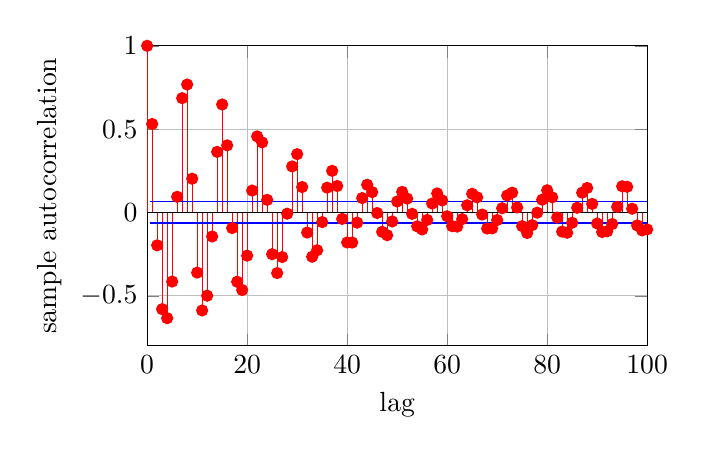
\begin{tikzpicture}

\begin{axis}[%
width=2.5in,
height=1.5in,
scale only axis,
xmin=0,
xmax=100,
xlabel={lag},
xmajorgrids,
ymin=-0.8,
ymax=1,
ylabel={sample autocorrelation},
ymajorgrids,
]
\addplot[ycomb,color=red,solid,mark size=2.0pt,mark=*,mark options={solid,fill=red}] plot table[row sep=crcr] {%
0	1\\
1	0.531012375277456\\
2	-0.19722744657221\\
3	-0.580093046226843\\
4	-0.634299361279394\\
5	-0.414510748215481\\
6	0.0940516998382318\\
7	0.685879732266424\\
8	0.767706341366509\\
9	0.202651503274669\\
10	-0.360753075814334\\
11	-0.587809692511437\\
12	-0.499374542532691\\
13	-0.144048742938735\\
14	0.363697338277312\\
15	0.647935296321381\\
16	0.402687846142643\\
17	-0.0936513180501337\\
18	-0.415641658040412\\
19	-0.465231628715779\\
20	-0.259047926027961\\
21	0.131616470574121\\
22	0.456403059036759\\
23	0.420665211089285\\
24	0.0757134794693025\\
25	-0.25029059785577\\
26	-0.363414909192172\\
27	-0.267448372946317\\
28	-0.00725311878350277\\
29	0.27641776758721\\
30	0.350147526867603\\
31	0.152519696142036\\
32	-0.120400195145866\\
33	-0.265388772684978\\
34	-0.226543296705639\\
35	-0.057524232662578\\
36	0.149038242145162\\
37	0.249893012712695\\
38	0.158918135972601\\
39	-0.0385093538827491\\
40	-0.17995280412447\\
41	-0.180326700511501\\
42	-0.0610913026777019\\
43	0.0864746394188238\\
44	0.166159947788355\\
45	0.122004495072026\\
46	-0.0033056106262259\\
47	-0.116431467216355\\
48	-0.136283669508414\\
49	-0.0538486021752314\\
50	0.0658938192822959\\
51	0.123492204764392\\
52	0.0833102007186009\\
53	-0.00824489146269923\\
54	-0.0832368116516709\\
55	-0.101938156163272\\
56	-0.0446236017196275\\
57	0.05381224724954\\
58	0.11444562311993\\
59	0.0723937663965338\\
60	-0.0226530416057325\\
61	-0.0821737593846169\\
62	-0.084963846753609\\
63	-0.0401676269139983\\
64	0.0432953457498929\\
65	0.112073757662789\\
66	0.0909093725544435\\
67	-0.0126049457164848\\
68	-0.0963090364883624\\
69	-0.0953149523683465\\
70	-0.0451934009589695\\
71	0.0254286808742385\\
72	0.101867891320578\\
73	0.118922313123251\\
74	0.0299211016844175\\
75	-0.0821706339376631\\
76	-0.123034935837922\\
77	-0.0760379895107557\\
78	-0.00119947423616588\\
79	0.0767222741387588\\
80	0.133366760645852\\
81	0.0907309328586872\\
82	-0.0303754385411401\\
83	-0.11484435701884\\
84	-0.121454231424134\\
85	-0.0615858654828823\\
86	0.0281677667722163\\
87	0.118911522175491\\
88	0.14719166655015\\
89	0.0513598687431599\\
90	-0.0661735316364488\\
91	-0.11720471472547\\
92	-0.112754441953474\\
93	-0.0693476056606004\\
94	0.0335169332028598\\
95	0.157044107441776\\
96	0.154067396062749\\
97	0.0226494900495964\\
98	-0.077591788580732\\
99	-0.107408975915327\\
100	-0.101719943568136\\
};
\addplot [color=blue,solid,forget plot]
  table[row sep=crcr]{%
0.5	0.0632455532033676\\
100	0.0632455532033676\\
};
\addplot [color=blue,solid,forget plot]
  table[row sep=crcr]{%
0.5	-0.0632455532033676\\
100	-0.0632455532033676\\
};
\addplot [color=black,solid,forget plot]
  table[row sep=crcr]{%
0	0\\
100	0\\
};
\end{axis}
\end{tikzpicture}%
\end{document}
% This file was created by matlab2tikz.
% Minimal pgfplots version: 1.3
%
%The latest updates can be retrieved from
%  http://www.mathworks.com/matlabcentral/fileexchange/22022-matlab2tikz
%where you can also make suggestions and rate matlab2tikz.
%
\documentclass[tikz]{standalone}
\usepackage{pgfplots}
\usepackage{grffile}
\pgfplotsset{compat=newest}
\usetikzlibrary{plotmarks}
\usepackage{amsmath}

\begin{document}
\definecolor{mycolor1}{rgb}{0.00000,0.44700,0.74100}%
%
\begin{tikzpicture}

\begin{axis}[%
width=1.5in,
height=1.5in,
scale only axis,
xmin=0,
xmax=100,
xlabel={delay},
ymode=log,
ymin=1e-05,
ymax=0.1,
yminorticks=true,
ylabel={$\log(\text{mse})$}
]
\addplot [color=mycolor1,solid,forget plot]
  table[row sep=crcr]{%
1	0.0216421324310104\\
2	0.00221305292322593\\
3	0.00141675042449202\\
4	0.00128957803361677\\
5	0.00122915823660737\\
6	0.00108528888355728\\
7	0.000866759084843548\\
8	0.000609590902422789\\
9	0.000526550388444512\\
10	0.000473711690269068\\
11	0.000454087567598411\\
12	0.000441644687190483\\
13	0.000426178636055369\\
14	0.000407814569638957\\
15	0.000355975650319363\\
16	0.000302831479183435\\
17	0.000245512053806742\\
18	0.000219221275661896\\
19	0.000213695079084987\\
20	0.000211690672604097\\
21	0.000207685576061439\\
22	0.000199054026492513\\
23	0.000180217511251245\\
24	0.000160703849591286\\
25	0.000140731230669125\\
26	0.000123927496556286\\
27	0.000117599867670577\\
28	0.000116737716848118\\
29	0.000114910356093006\\
30	0.000112016301862051\\
31	0.000105908633547843\\
32	0.000100180698641329\\
33	9.01550837703955e-05\\
34	8.140543436947e-05\\
35	7.75881182031642e-05\\
36	7.65730731494018e-05\\
37	7.58557934652492e-05\\
38	7.3909691187114e-05\\
39	7.08749074461454e-05\\
40	6.72399847187632e-05\\
41	6.2078016558049e-05\\
42	5.77202532836098e-05\\
43	5.59710996876075e-05\\
44	5.53278629746288e-05\\
45	5.4948487217007e-05\\
46	5.34839122512813e-05\\
47	5.13993323980418e-05\\
48	4.81924934100017e-05\\
49	4.55378112740019e-05\\
50	4.34060640498578e-05\\
51	4.25972145831045e-05\\
52	4.22386708056718e-05\\
53	4.19026412857837e-05\\
54	4.07850538674497e-05\\
55	3.95676901971669e-05\\
56	3.70850657026003e-05\\
57	3.54849413646843e-05\\
58	3.43250972579767e-05\\
59	3.38677177645602e-05\\
60	3.38420548456265e-05\\
61	3.30864603688085e-05\\
62	3.24268180095363e-05\\
63	3.12026672962434e-05\\
64	2.98403080311486e-05\\
65	2.88045071744304e-05\\
66	2.81843110527059e-05\\
67	2.78994482759121e-05\\
68	2.78007363869147e-05\\
69	2.71472040396445e-05\\
70	2.64030063359459e-05\\
71	2.52561827522698e-05\\
72	2.43174088263536e-05\\
73	2.37073488569417e-05\\
74	2.34872513363761e-05\\
75	2.33114083845021e-05\\
76	2.3267886749536e-05\\
77	2.28064770085052e-05\\
78	2.19841442057876e-05\\
79	2.1235684901193e-05\\
80	2.06032369018838e-05\\
81	2.02103012705342e-05\\
82	2.00975780220547e-05\\
83	1.9890022061235e-05\\
84	1.94290478123916e-05\\
85	1.87596904870069e-05\\
86	1.81263639869375e-05\\
87	1.76881033483402e-05\\
88	1.72387877943012e-05\\
89	1.70878929755738e-05\\
90	1.69621340676102e-05\\
91	1.66134983148009e-05\\
92	1.65248848919495e-05\\
93	1.6497092412055e-05\\
94	1.61630398578886e-05\\
95	1.5855387285132e-05\\
96	1.55590068045134e-05\\
97	1.55104877681064e-05\\
98	1.54040224134284e-05\\
99	1.52184925665193e-05\\
100	1.5012045075635e-05\\
};
\end{axis}
\end{tikzpicture}%
\end{document}
\caption{Autocorrelation analysis of the training time-series shown with 95\% confidence bounds (left). Training set error using an svm trained using $\gamma = 75.5, \sigma^2 = 27.8$ and a linearly increasing window size.}
\label{fig:santaFeAutocorr}
\end{figure}
In order to choose the window size the sample autocorrelation function shown in figure~\ref{fig:santaFeAutocorr} is considered. In the plot the autocorrelation values start to come close to the confidence bounds around a lag of fifty samples. Therefore a window size of fifty will be used as this shift covers the most significant samples. The plot on the right of figure~\ref{fig:santaFeAutocorr} confirms this choice as reasonable when a window size of fifty samples is reached the error has already fallen over three decades. From fifty to hundred the error falls only by about one more decade. Thus choosing fifty as window size covers the most important part of the information present. \\
\begin{figure}
\centering
\tikzset{mark size=1}
% This file was created by matlab2tikz.
% Minimal pgfplots version: 1.3
%
%The latest updates can be retrieved from
%  http://www.mathworks.com/matlabcentral/fileexchange/22022-matlab2tikz
%where you can also make suggestions and rate matlab2tikz.
%
\documentclass[tikz]{standalone}
\usepackage{pgfplots}
\usepackage{grffile}
\pgfplotsset{compat=newest}
\usetikzlibrary{plotmarks}
\usepackage{amsmath}

\begin{document}
\definecolor{mycolor1}{rgb}{0.00000,0.44700,0.74100}%
\definecolor{mycolor2}{rgb}{0.85000,0.32500,0.09800}%
\definecolor{mycolor3}{rgb}{0.92900,0.69400,0.12500}%
%
\begin{tikzpicture}

\begin{axis}[%
width=3.5in,
height=1.5in,
scale only axis,
xmin=0,
xmax=200,
ymin=0.0,
ymax=1
]
\addplot [color=mycolor1,solid,forget plot]
  table[row sep=crcr]{%
1	0.287937743190661\\
2	0.700389105058366\\
3	0.482490272373541\\
4	0.147859922178988\\
5	0.0622568093385214\\
6	0.0505836575875486\\
7	0.0622568093385214\\
8	0.132295719844358\\
9	0.43579766536965\\
10	0.739299610894942\\
11	0.319066147859922\\
12	0.0972762645914397\\
13	0.0544747081712062\\
14	0.0466926070038911\\
15	0.066147859922179\\
16	0.182879377431907\\
17	0.595330739299611\\
18	0.665369649805447\\
19	0.214007782101167\\
20	0.0778210116731518\\
21	0.0544747081712062\\
22	0.0428015564202335\\
23	0.0739299610894942\\
24	0.24124513618677\\
25	0.715953307392996\\
26	0.56420233463035\\
27	0.155642023346304\\
28	0.0583657587548638\\
29	0.0428015564202335\\
30	0.0428015564202335\\
31	0.0817120622568093\\
32	0.284046692607004\\
33	0.78988326848249\\
34	0.498054474708171\\
35	0.124513618677043\\
36	0.0544747081712062\\
37	0.0428015564202335\\
38	0.0389105058365759\\
39	0.0778210116731518\\
40	0.280155642023346\\
41	0.828793774319066\\
42	0.517509727626459\\
43	0.124513618677043\\
44	0.0505836575875486\\
45	0.0389105058365759\\
46	0.0389105058365759\\
47	0.0583657587548638\\
48	0.190661478599222\\
49	0.754863813229572\\
50	0.704280155642023\\
51	0.163424124513619\\
52	0.0583657587548638\\
53	0.0428015564202335\\
54	0.0350194552529183\\
55	0.0350194552529183\\
56	0.0622568093385214\\
57	0.284046692607004\\
58	1\\
59	0.517509727626459\\
60	0.101167315175097\\
61	0.0428015564202335\\
62	0.0350194552529183\\
63	0.0350194552529183\\
64	0.0272373540856031\\
65	0.0233463035019455\\
66	0.0194552529182879\\
67	0.0389105058365759\\
68	0.0856031128404669\\
69	0.0583657587548638\\
70	0.0466926070038911\\
71	0.0583657587548638\\
72	0.0856031128404669\\
73	0.1284046692607\\
74	0.171206225680934\\
75	0.229571984435798\\
76	0.272373540856031\\
77	0.280155642023346\\
78	0.237354085603113\\
79	0.194552529182879\\
80	0.186770428015564\\
81	0.206225680933852\\
82	0.245136186770428\\
83	0.280155642023346\\
84	0.268482490272374\\
85	0.229571984435798\\
86	0.194552529182879\\
87	0.190661478599222\\
88	0.214007782101167\\
89	0.260700389105058\\
90	0.287937743190661\\
91	0.268482490272374\\
92	0.229571984435798\\
93	0.190661478599222\\
94	0.190661478599222\\
95	0.217898832684825\\
96	0.268482490272374\\
97	0.291828793774319\\
98	0.264591439688716\\
99	0.217898832684825\\
100	0.194552529182879\\
101	0.190661478599222\\
102	0.221789883268482\\
103	0.272373540856031\\
104	0.295719844357977\\
105	0.260700389105058\\
106	0.217898832684825\\
107	0.186770428015564\\
108	0.194552529182879\\
109	0.229571984435798\\
110	0.280155642023346\\
111	0.299610894941634\\
112	0.260700389105058\\
113	0.21011673151751\\
114	0.182879377431907\\
115	0.190661478599222\\
116	0.233463035019455\\
117	0.287937743190661\\
118	0.295719844357977\\
119	0.256809338521401\\
120	0.202334630350195\\
121	0.178988326848249\\
122	0.190661478599222\\
123	0.24124513618677\\
124	0.295719844357977\\
125	0.303501945525292\\
126	0.252918287937743\\
127	0.194552529182879\\
128	0.178988326848249\\
129	0.194552529182879\\
130	0.245136186770428\\
131	0.307392996108949\\
132	0.307392996108949\\
133	0.245136186770428\\
134	0.194552529182879\\
135	0.175097276264591\\
136	0.194552529182879\\
137	0.256809338521401\\
138	0.315175097276265\\
139	0.307392996108949\\
140	0.24124513618677\\
141	0.190661478599222\\
142	0.171206225680934\\
143	0.198443579766537\\
144	0.268482490272374\\
145	0.326848249027237\\
146	0.307392996108949\\
147	0.233463035019455\\
148	0.182879377431907\\
149	0.171206225680934\\
150	0.206225680933852\\
151	0.276264591439689\\
152	0.334630350194553\\
153	0.307392996108949\\
154	0.22568093385214\\
155	0.175097276264591\\
156	0.171206225680934\\
157	0.21011673151751\\
158	0.287937743190661\\
159	0.342412451361868\\
160	0.307392996108949\\
161	0.22568093385214\\
162	0.171206225680934\\
163	0.171206225680934\\
164	0.217898832684825\\
165	0.295719844357977\\
166	0.350194552529183\\
167	0.303501945525292\\
168	0.217898832684825\\
169	0.167315175097276\\
170	0.171206225680934\\
171	0.221789883268482\\
172	0.311284046692607\\
173	0.357976653696498\\
174	0.299610894941634\\
175	0.21011673151751\\
176	0.167315175097276\\
177	0.167315175097276\\
178	0.22568093385214\\
179	0.32295719844358\\
180	0.365758754863813\\
181	0.295719844357977\\
182	0.206225680933852\\
183	0.159533073929961\\
184	0.171206225680934\\
185	0.229571984435798\\
186	0.330739299610895\\
187	0.373540856031128\\
188	0.287937743190661\\
189	0.198443579766537\\
190	0.155642023346304\\
191	0.171206225680934\\
192	0.233463035019455\\
193	0.342412451361868\\
194	0.377431906614786\\
195	0.280155642023346\\
196	0.190661478599222\\
197	0.147859922178988\\
198	0.163424124513619\\
199	0.237354085603113\\
200	0.35408560311284\\
};
\addplot [color=mycolor2,solid,forget plot]
  table[row sep=crcr]{%
1	0.290391387395838\\
2	0.701029557319766\\
3	0.483057043747828\\
4	0.154365637761923\\
5	0.0666086620113165\\
6	0.0501728269701258\\
7	0.0624047693455013\\
8	0.13432149654308\\
9	0.438107265537285\\
10	0.744097336941653\\
11	0.324895775106589\\
12	0.102278290803843\\
13	0.0556316238006404\\
14	0.050127620629275\\
15	0.0708298200621928\\
16	0.185080798125813\\
17	0.591094563213807\\
18	0.674939639698209\\
19	0.224785700746731\\
20	0.0739966714311767\\
21	0.0467375909063907\\
22	0.0465758575966532\\
23	0.076630277451799\\
24	0.239753486596926\\
25	0.708488176558831\\
26	0.585671527916416\\
27	0.16685390145932\\
28	0.0613533518889921\\
29	0.0439676966563466\\
30	0.0461910110167242\\
31	0.0808843476096627\\
32	0.274951461218364\\
33	0.770355553076368\\
34	0.536328451412344\\
35	0.134939099702276\\
36	0.0501031468178613\\
37	0.0394734293237683\\
38	0.0366351101993837\\
39	0.0712984899177717\\
40	0.254887084035749\\
41	0.787110303187066\\
42	0.584731318205248\\
43	0.136908530265657\\
44	0.0508296081752361\\
45	0.036702859947774\\
46	0.0305576987962545\\
47	0.04951090730705\\
48	0.160195465588631\\
49	0.638427556196384\\
50	0.855231279975158\\
51	0.205254071111674\\
52	0.0508091911443878\\
53	0.0368170542044121\\
54	0.0309329466286221\\
55	0.0268775608526285\\
56	0.0406079387272041\\
57	0.15736677480282\\
58	0.714186992968067\\
59	0.58968610233935\\
60	0.254497975013861\\
61	0.0423374968407262\\
62	0.00930888713924219\\
63	0.0101810712763414\\
64	0.0193496011420315\\
65	0.0749564180199652\\
66	0.0543161126177958\\
67	0.0348641836842875\\
68	0.219148410832293\\
69	0.163518183034531\\
70	0.0827454569449873\\
71	0.0702649019273583\\
72	0.106646726060072\\
73	0.173372056728336\\
74	0.27020161220009\\
75	0.355027426328402\\
76	0.298587655851796\\
77	0.163082649524849\\
78	0.160793786905344\\
79	0.200711546155201\\
80	0.250656568258795\\
81	0.290439503627947\\
82	0.317634032596406\\
83	0.257055921411974\\
84	0.19743198617071\\
85	0.158667869905126\\
86	0.201849201568171\\
87	0.249305994629114\\
88	0.288178529305654\\
89	0.309277723467985\\
90	0.263374582372061\\
91	0.194341910796043\\
92	0.171706366828728\\
93	0.202180218128379\\
94	0.254805526347611\\
95	0.302516813167252\\
96	0.300255038094762\\
97	0.253019369769928\\
98	0.201058781147157\\
99	0.181668461547233\\
100	0.201954525740478\\
101	0.258973774521654\\
102	0.316904893177288\\
103	0.313703752697108\\
104	0.243361788438698\\
105	0.196628722143247\\
106	0.189952118570169\\
107	0.210588025910655\\
108	0.269304665794855\\
109	0.325118259021932\\
110	0.303258888336713\\
111	0.230303509421868\\
112	0.182660458802993\\
113	0.18104095104289\\
114	0.212710171535161\\
115	0.278697077184316\\
116	0.333762172098188\\
117	0.299029089312531\\
118	0.229394272478611\\
119	0.183359082406352\\
120	0.178817313096002\\
121	0.214142866440125\\
122	0.28905652131744\\
123	0.342470315981969\\
124	0.301551300523095\\
125	0.220076546411602\\
126	0.179116876996908\\
127	0.176915114929046\\
128	0.219238452144026\\
129	0.298293189199546\\
130	0.351196645861553\\
131	0.296982139300177\\
132	0.214670795315536\\
133	0.171361038306001\\
134	0.175144988354055\\
135	0.222216014746566\\
136	0.308868831401286\\
137	0.357731466454167\\
138	0.292373910994868\\
139	0.206484371556811\\
140	0.166128391819814\\
141	0.172412060709784\\
142	0.225972625191485\\
143	0.319828753858112\\
144	0.363107002260094\\
145	0.287765999398907\\
146	0.199636997644854\\
147	0.161608959507855\\
148	0.170278743619969\\
149	0.231150322819538\\
150	0.33045175758305\\
151	0.369489752240588\\
152	0.281929438489484\\
153	0.193364935872142\\
154	0.15647211217402\\
155	0.168406723079809\\
156	0.234921639018199\\
157	0.341890180390998\\
158	0.374701518826543\\
159	0.276659500425492\\
160	0.185748165978849\\
161	0.151788215084416\\
162	0.166550679778251\\
163	0.238831600428427\\
164	0.352353083124605\\
165	0.378973627264565\\
166	0.271269755725509\\
167	0.179128421456343\\
168	0.147217123786929\\
169	0.164449217266604\\
170	0.242592736953792\\
171	0.362232775673046\\
172	0.383778262158739\\
173	0.266071063257028\\
174	0.17336933243557\\
175	0.142637663159083\\
176	0.162410807641045\\
177	0.245227281148023\\
178	0.372073852664147\\
179	0.388082972871163\\
180	0.262239413306324\\
181	0.167563125321007\\
182	0.138540861061359\\
183	0.159625729713699\\
184	0.247221168177362\\
185	0.380816590531905\\
186	0.393022464423036\\
187	0.259131572088633\\
188	0.162596325455562\\
189	0.134316473719436\\
190	0.156537707389075\\
191	0.247980427093435\\
192	0.388526216830554\\
193	0.39875059797291\\
194	0.257241752986229\\
195	0.158394607417351\\
196	0.130241502273668\\
197	0.153105153126653\\
198	0.247065410302028\\
199	0.395211481330239\\
200	0.405483560079441\\
};
\addplot [color=mycolor3,only marks,mark=*,mark options={solid},forget plot]
  table[row sep=crcr]{%
1	0.00245364420517624\\
2	0.000640452261400304\\
3	0.000566771374286679\\
4	0.00650571558293464\\
5	0.00435185267279509\\
6	0.000410830617422878\\
7	0.000147960006979864\\
8	0.00202577669872187\\
9	0.00230960016763559\\
10	0.00479772604671158\\
11	0.00582962724666702\\
12	0.00500202621240352\\
13	0.00115691562943412\\
14	0.00343501362538393\\
15	0.00468196014001386\\
16	0.00220142069390661\\
17	0.00423617608580429\\
18	0.00956998989276125\\
19	0.0107779186455634\\
20	0.003824340241975\\
21	0.00773711726481549\\
22	0.00377430117641976\\
23	0.00270031636230482\\
24	0.00149164958984466\\
25	0.00746513083416533\\
26	0.0214691932860657\\
27	0.0112118781130162\\
28	0.00298759313412829\\
29	0.0011661402361131\\
30	0.00338945459649072\\
31	0.000827714647146635\\
32	0.00909523138863993\\
33	0.0195277154061226\\
34	0.0382739767041725\\
35	0.0104254810252335\\
36	0.00437156135334496\\
37	0.00332812709646514\\
38	0.0022753956371922\\
39	0.00652252175538004\\
40	0.0252685579875978\\
41	0.0416834711320004\\
42	0.0672215905787893\\
43	0.0123949115886146\\
44	0.000245950587687491\\
45	0.00220764588880187\\
46	0.0083528070403214\\
47	0.00885485144781377\\
48	0.0304660130105909\\
49	0.116436257033188\\
50	0.150951124333134\\
51	0.0418299465980551\\
52	0.00755656761047598\\
53	0.00598450221582141\\
54	0.0040865086242962\\
55	0.0081418944002898\\
56	0.0216488706113173\\
57	0.126679917804184\\
58	0.285813007031933\\
59	0.0721763747128912\\
60	0.153330659838764\\
61	0.000464059579507278\\
62	0.0257105681136761\\
63	0.0248383839765769\\
64	0.00788775294357157\\
65	0.0516101145180197\\
66	0.0348608596995078\\
67	0.00404632215228837\\
68	0.133545297991826\\
69	0.105152424279667\\
70	0.0360528499410963\\
71	0.0118991431724945\\
72	0.0210436132196049\\
73	0.044967387467636\\
74	0.0989953865191559\\
75	0.125455441892605\\
76	0.0262141149957649\\
77	0.117072992498498\\
78	0.0765602986977686\\
79	0.00615901697232196\\
80	0.0638861402432308\\
81	0.0842138226940949\\
82	0.0724978458259784\\
83	0.0230997206113727\\
84	0.0710505041016634\\
85	0.0709041145306716\\
86	0.00729667238529119\\
87	0.0586445160298923\\
88	0.0741707472044869\\
89	0.0485773343629264\\
90	0.0245631608186009\\
91	0.0741405794763301\\
92	0.0578656176070692\\
93	0.0115187395291572\\
94	0.0641440477483893\\
95	0.0846179804824273\\
96	0.0317725478223888\\
97	0.0388094240043909\\
98	0.0635326585415593\\
99	0.036230371137592\\
100	0.00740199655759821\\
101	0.0683122959224323\\
102	0.0951150099088055\\
103	0.0413302118410766\\
104	0.0523580559192787\\
105	0.0640716669618119\\
106	0.0279467141146558\\
107	0.0238175978950906\\
108	0.0747521366119756\\
109	0.0955462745861347\\
110	0.0231032463133669\\
111	0.0693073855197666\\
112	0.0780399303020656\\
113	0.0290757804746195\\
114	0.0298307941032547\\
115	0.0880355985850944\\
116	0.100299137078733\\
117	0.01109134612187\\
118	0.0663255718793657\\
119	0.073450256115049\\
120	0.0235173172541921\\
121	0.0351545395918759\\
122	0.0983950427182183\\
123	0.101225179795198\\
124	0.00583145616511865\\
125	0.0834253991136899\\
126	0.0738014109408355\\
127	0.0176374142538329\\
128	0.040250125295777\\
129	0.103740660016667\\
130	0.106060459091125\\
131	0.0104108568087729\\
132	0.092722200793413\\
133	0.0737751484644269\\
134	0.0194075408288241\\
135	0.0471187384819745\\
136	0.114316302218406\\
137	0.100922127932767\\
138	0.0228011862813967\\
139	0.100908624552139\\
140	0.0751167443669566\\
141	0.0182494178894375\\
142	0.054766399510551\\
143	0.121385174091575\\
144	0.0946245119877206\\
145	0.0390822496283305\\
146	0.107755998464095\\
147	0.0718540755116003\\
148	0.0126006338119379\\
149	0.0599440971386045\\
150	0.124226076649198\\
151	0.093225160800899\\
152	0.0527009117050686\\
153	0.114028060236807\\
154	0.0692088216781196\\
155	0.00669055318478237\\
156	0.0637154133372649\\
157	0.131773448873488\\
158	0.0867637756358811\\
159	0.065752950936376\\
160	0.121644830130101\\
161	0.0738927187677245\\
162	0.00465554590268302\\
163	0.0676253747474931\\
164	0.13445425043978\\
165	0.0832537829065884\\
166	0.0789247968036734\\
167	0.124373524068949\\
168	0.0706817088978963\\
169	0.00286595783067273\\
170	0.0713865112728582\\
171	0.140442892404564\\
172	0.0724942154661322\\
173	0.0919055904394703\\
174	0.126241562506064\\
175	0.0674790683584267\\
176	0.00490436745623121\\
177	0.0779121060507466\\
178	0.146392918812007\\
179	0.0651257744275831\\
180	0.103519341557489\\
181	0.12815671903697\\
182	0.0676848198724934\\
183	9.26557837377107e-05\\
184	0.0760149424964286\\
185	0.151244606096107\\
186	0.0622831648121408\\
187	0.114409283942496\\
188	0.125341417735099\\
189	0.0641271060471014\\
190	0.000895684042771794\\
191	0.0767742014125011\\
192	0.155063181811099\\
193	0.0563381466110423\\
194	0.120190153628557\\
195	0.121761034605995\\
196	0.0604199763255536\\
197	0.00524523094766427\\
198	0.0836412857884095\\
199	0.157857395727126\\
200	0.0513979569666009\\
};
\end{axis}
\end{tikzpicture}%
\end{document}
% This file was created by matlab2tikz.
% Minimal pgfplots version: 1.3
%
%The latest updates can be retrieved from
%  http://www.mathworks.com/matlabcentral/fileexchange/22022-matlab2tikz
%where you can also make suggestions and rate matlab2tikz.
%
\documentclass[tikz]{standalone}
\usepackage{pgfplots}
\usepackage{grffile}
\pgfplotsset{compat=newest}
\usetikzlibrary{plotmarks}
\usepackage{amsmath}

\begin{document}
\definecolor{mycolor1}{rgb}{0.00000,0.44700,0.74100}%
\definecolor{mycolor2}{rgb}{0.85000,0.32500,0.09800}%
\definecolor{mycolor3}{rgb}{0.92900,0.69400,0.12500}%
%
\begin{tikzpicture}

\begin{axis}[%
width=3.5in,
height=1.5in,
scale only axis,
xmin=0,
xmax=200,
ymin=0,
ymax=1
]
\addplot [color=mycolor1,solid,forget plot]
  table[row sep=crcr]{%
1	0.287937743190661\\
2	0.700389105058366\\
3	0.482490272373541\\
4	0.147859922178988\\
5	0.0622568093385214\\
6	0.0505836575875486\\
7	0.0622568093385214\\
8	0.132295719844358\\
9	0.43579766536965\\
10	0.739299610894942\\
11	0.319066147859922\\
12	0.0972762645914397\\
13	0.0544747081712062\\
14	0.0466926070038911\\
15	0.066147859922179\\
16	0.182879377431907\\
17	0.595330739299611\\
18	0.665369649805447\\
19	0.214007782101167\\
20	0.0778210116731518\\
21	0.0544747081712062\\
22	0.0428015564202335\\
23	0.0739299610894942\\
24	0.24124513618677\\
25	0.715953307392996\\
26	0.56420233463035\\
27	0.155642023346304\\
28	0.0583657587548638\\
29	0.0428015564202335\\
30	0.0428015564202335\\
31	0.0817120622568093\\
32	0.284046692607004\\
33	0.78988326848249\\
34	0.498054474708171\\
35	0.124513618677043\\
36	0.0544747081712062\\
37	0.0428015564202335\\
38	0.0389105058365759\\
39	0.0778210116731518\\
40	0.280155642023346\\
41	0.828793774319066\\
42	0.517509727626459\\
43	0.124513618677043\\
44	0.0505836575875486\\
45	0.0389105058365759\\
46	0.0389105058365759\\
47	0.0583657587548638\\
48	0.190661478599222\\
49	0.754863813229572\\
50	0.704280155642023\\
51	0.163424124513619\\
52	0.0583657587548638\\
53	0.0428015564202335\\
54	0.0350194552529183\\
55	0.0350194552529183\\
56	0.0622568093385214\\
57	0.284046692607004\\
58	1\\
59	0.517509727626459\\
60	0.101167315175097\\
61	0.0428015564202335\\
62	0.0350194552529183\\
63	0.0350194552529183\\
64	0.0272373540856031\\
65	0.0233463035019455\\
66	0.0194552529182879\\
67	0.0389105058365759\\
68	0.0856031128404669\\
69	0.0583657587548638\\
70	0.0466926070038911\\
71	0.0583657587548638\\
72	0.0856031128404669\\
73	0.1284046692607\\
74	0.171206225680934\\
75	0.229571984435798\\
76	0.272373540856031\\
77	0.280155642023346\\
78	0.237354085603113\\
79	0.194552529182879\\
80	0.186770428015564\\
81	0.206225680933852\\
82	0.245136186770428\\
83	0.280155642023346\\
84	0.268482490272374\\
85	0.229571984435798\\
86	0.194552529182879\\
87	0.190661478599222\\
88	0.214007782101167\\
89	0.260700389105058\\
90	0.287937743190661\\
91	0.268482490272374\\
92	0.229571984435798\\
93	0.190661478599222\\
94	0.190661478599222\\
95	0.217898832684825\\
96	0.268482490272374\\
97	0.291828793774319\\
98	0.264591439688716\\
99	0.217898832684825\\
100	0.194552529182879\\
101	0.190661478599222\\
102	0.221789883268482\\
103	0.272373540856031\\
104	0.295719844357977\\
105	0.260700389105058\\
106	0.217898832684825\\
107	0.186770428015564\\
108	0.194552529182879\\
109	0.229571984435798\\
110	0.280155642023346\\
111	0.299610894941634\\
112	0.260700389105058\\
113	0.21011673151751\\
114	0.182879377431907\\
115	0.190661478599222\\
116	0.233463035019455\\
117	0.287937743190661\\
118	0.295719844357977\\
119	0.256809338521401\\
120	0.202334630350195\\
121	0.178988326848249\\
122	0.190661478599222\\
123	0.24124513618677\\
124	0.295719844357977\\
125	0.303501945525292\\
126	0.252918287937743\\
127	0.194552529182879\\
128	0.178988326848249\\
129	0.194552529182879\\
130	0.245136186770428\\
131	0.307392996108949\\
132	0.307392996108949\\
133	0.245136186770428\\
134	0.194552529182879\\
135	0.175097276264591\\
136	0.194552529182879\\
137	0.256809338521401\\
138	0.315175097276265\\
139	0.307392996108949\\
140	0.24124513618677\\
141	0.190661478599222\\
142	0.171206225680934\\
143	0.198443579766537\\
144	0.268482490272374\\
145	0.326848249027237\\
146	0.307392996108949\\
147	0.233463035019455\\
148	0.182879377431907\\
149	0.171206225680934\\
150	0.206225680933852\\
151	0.276264591439689\\
152	0.334630350194553\\
153	0.307392996108949\\
154	0.22568093385214\\
155	0.175097276264591\\
156	0.171206225680934\\
157	0.21011673151751\\
158	0.287937743190661\\
159	0.342412451361868\\
160	0.307392996108949\\
161	0.22568093385214\\
162	0.171206225680934\\
163	0.171206225680934\\
164	0.217898832684825\\
165	0.295719844357977\\
166	0.350194552529183\\
167	0.303501945525292\\
168	0.217898832684825\\
169	0.167315175097276\\
170	0.171206225680934\\
171	0.221789883268482\\
172	0.311284046692607\\
173	0.357976653696498\\
174	0.299610894941634\\
175	0.21011673151751\\
176	0.167315175097276\\
177	0.167315175097276\\
178	0.22568093385214\\
179	0.32295719844358\\
180	0.365758754863813\\
181	0.295719844357977\\
182	0.206225680933852\\
183	0.159533073929961\\
184	0.171206225680934\\
185	0.229571984435798\\
186	0.330739299610895\\
187	0.373540856031128\\
188	0.287937743190661\\
189	0.198443579766537\\
190	0.155642023346304\\
191	0.171206225680934\\
192	0.233463035019455\\
193	0.342412451361868\\
194	0.377431906614786\\
195	0.280155642023346\\
196	0.190661478599222\\
197	0.147859922178988\\
198	0.163424124513619\\
199	0.237354085603113\\
200	0.35408560311284\\
};
\addplot [color=mycolor2,solid,forget plot]
  table[row sep=crcr]{%
1	0.291886869228443\\
2	0.697130726731448\\
3	0.487799517158665\\
4	0.154774877019776\\
5	0.0649354193559451\\
6	0.0494689776532875\\
7	0.0622211250534412\\
8	0.133790172612665\\
9	0.439045015501186\\
10	0.741296755625048\\
11	0.324459566114609\\
12	0.104504614984293\\
13	0.0553617505128097\\
14	0.0495722203999687\\
15	0.0701554166143887\\
16	0.18540737023975\\
17	0.588806323031377\\
18	0.681674407410467\\
19	0.218943319946057\\
20	0.0722517312762941\\
21	0.0454905216331989\\
22	0.0466996782981562\\
23	0.07590612017735\\
24	0.240824815754049\\
25	0.702525346705381\\
26	0.596658586733029\\
27	0.161894653061468\\
28	0.0616341779215883\\
29	0.0433290672730867\\
30	0.0452146367491821\\
31	0.0802024024926485\\
32	0.276353732989184\\
33	0.761039308806729\\
34	0.554968094478045\\
35	0.132778254832576\\
36	0.0513670936443507\\
37	0.0384154601938425\\
38	0.0364137827996357\\
39	0.0707994850994975\\
40	0.256014874444811\\
41	0.761981244166447\\
42	0.621590404190769\\
43	0.143252736104326\\
44	0.0509496210753744\\
45	0.0363653806427595\\
46	0.0301100343214265\\
47	0.0492643271850693\\
48	0.156905881495576\\
49	0.598403051948812\\
50	0.879675355297601\\
51	0.229833508816847\\
52	0.0537787267090907\\
53	0.0360416918114368\\
54	0.0285121116569129\\
55	0.0280485373213473\\
56	0.0371421695182688\\
57	0.158970393570298\\
58	0.630413455946958\\
59	0.578609832904323\\
60	0.315254080824035\\
61	0.0530594721829632\\
62	0.0106088775040281\\
63	0.0150289680166378\\
64	0.0260390889042243\\
65	0.094725792111361\\
66	0.0885148473395054\\
67	0.0969655099947817\\
68	0.328561586133897\\
69	0.219766029762373\\
70	0.104172820171157\\
71	0.0830862103737487\\
72	0.124668003269277\\
73	0.194547025526097\\
74	0.286557076498616\\
75	0.389930128544149\\
76	0.371572614563561\\
77	0.164191783085857\\
78	0.140188650686886\\
79	0.179935943578036\\
80	0.239265956551433\\
81	0.298210826561904\\
82	0.352478654507743\\
83	0.316713010608256\\
84	0.242856129897474\\
85	0.142212198387658\\
86	0.170220282232791\\
87	0.22307911836009\\
88	0.284374100528503\\
89	0.337545618750158\\
90	0.313531819131156\\
91	0.243671476623087\\
92	0.174463554111852\\
93	0.16478514226028\\
94	0.217985461527671\\
95	0.290014834145011\\
96	0.323686802806832\\
97	0.302512810257594\\
98	0.254000765964999\\
99	0.198247679185648\\
100	0.168548364601543\\
101	0.207004958208068\\
102	0.296239784700953\\
103	0.340261237366632\\
104	0.295720166677682\\
105	0.247554192280746\\
106	0.219694377319942\\
107	0.189752322151385\\
108	0.211345525025351\\
109	0.290779162152801\\
110	0.340784669309231\\
111	0.291804234813182\\
112	0.231799055608591\\
113	0.205384152875912\\
114	0.199991495167201\\
115	0.225728650952047\\
116	0.290436754187828\\
117	0.333368290430046\\
118	0.306374474346272\\
119	0.23698713191375\\
120	0.199334067766042\\
121	0.200362215331887\\
122	0.236623255888904\\
123	0.2942221411035\\
124	0.335271925860197\\
125	0.302708262506278\\
126	0.238849581078997\\
127	0.197053395169444\\
128	0.1976554720901\\
129	0.238362278536101\\
130	0.302204902590099\\
131	0.335557143406162\\
132	0.300387383168526\\
133	0.234249353104478\\
134	0.196058268946134\\
135	0.196971073659317\\
136	0.239961146649698\\
137	0.307897659807763\\
138	0.337595224220046\\
139	0.294791876844628\\
140	0.230019686908917\\
141	0.194366612290787\\
142	0.19747164893116\\
143	0.242806492024891\\
144	0.311770989826536\\
145	0.340476013543803\\
146	0.289526567860604\\
147	0.224551871520425\\
148	0.192277816996463\\
149	0.199831644010913\\
150	0.247053202537272\\
151	0.316942573220909\\
152	0.341853724083972\\
153	0.285065515976205\\
154	0.218569427452066\\
155	0.189302928245652\\
156	0.200605300576123\\
157	0.251986428887872\\
158	0.323470141053304\\
159	0.342875858999844\\
160	0.279753954963934\\
161	0.213284887386943\\
162	0.186682343556792\\
163	0.20066766003998\\
164	0.256722802471902\\
165	0.330169697096791\\
166	0.343455242047821\\
167	0.27315902677445\\
168	0.208158573561525\\
169	0.184343635808928\\
170	0.201479297918338\\
171	0.261302052239579\\
172	0.33713052661746\\
173	0.343133103885865\\
174	0.266833618355779\\
175	0.202690621255063\\
176	0.18191067914461\\
177	0.202363557121287\\
178	0.266750869283501\\
179	0.343749936528164\\
180	0.342478793635838\\
181	0.260183967232131\\
182	0.197434083783726\\
183	0.179303292357947\\
184	0.203324147022125\\
185	0.27253588923457\\
186	0.35049690180924\\
187	0.341077220827622\\
188	0.253615055559763\\
189	0.192292089438201\\
190	0.176642391843989\\
191	0.204363887233555\\
192	0.27851476786999\\
193	0.357389373720835\\
194	0.339000718225207\\
195	0.247180582725258\\
196	0.187322149608605\\
197	0.174097962990502\\
198	0.205333210683501\\
199	0.284704190037119\\
200	0.364113234179249\\
};
\addplot [color=mycolor3,only marks,mark=*,mark options={solid},forget plot]
  table[row sep=crcr]{%
1	0.00394912603778175\\
2	0.00325837832691755\\
3	0.00530924478512451\\
4	0.00691495484078772\\
5	0.0026786100174237\\
6	0.00111467993426116\\
7	3.56842850801897e-05\\
8	0.00149445276830687\\
9	0.00324735013153615\\
10	0.0019971447301067\\
11	0.00539341825468709\\
12	0.0072283503928534\\
13	0.000887042341603472\\
14	0.00287961339607762\\
15	0.00400755669220972\\
16	0.00252799280784313\\
17	0.00652441626823375\\
18	0.0163047576050193\\
19	0.00493553784488976\\
20	0.0055692803968577\\
21	0.00898418653800728\\
22	0.00389812187792278\\
23	0.00197615908785585\\
24	0.000420320432721305\\
25	0.0134279606876146\\
26	0.032456252102679\\
27	0.0062526297151641\\
28	0.00326841916672445\\
29	0.0005275108528532\\
30	0.00241308032894859\\
31	0.00150965976416083\\
32	0.00769295961782035\\
33	0.0288439596757611\\
34	0.0569136197698733\\
35	0.00826463615553324\\
36	0.00310761452685557\\
37	0.00438609622639101\\
38	0.00249672303694021\\
39	0.00702152657365426\\
40	0.0241407675785357\\
41	0.0668125301526197\\
42	0.10408067656431\\
43	0.0187391174272831\\
44	0.000365963487825763\\
45	0.00254512519381636\\
46	0.00880047151514937\\
47	0.00910143156979452\\
48	0.0337555971036458\\
49	0.15646076128076\\
50	0.175395199655578\\
51	0.0664093843032284\\
52	0.00458703204577314\\
53	0.00675986460879661\\
54	0.0065073435960054\\
55	0.00697091793157102\\
56	0.0251146398202526\\
57	0.125076299036706\\
58	0.369586544053042\\
59	0.0611001052778639\\
60	0.214086765648938\\
61	0.0102579157627297\\
62	0.0244105777488902\\
63	0.0199904872362805\\
64	0.00119826518137879\\
65	0.0713794886094155\\
66	0.0690595944212174\\
67	0.0580550041582059\\
68	0.24295847329343\\
69	0.161400271007509\\
70	0.0574802131672664\\
71	0.0247204516188849\\
72	0.0390648904288101\\
73	0.0661423562653964\\
74	0.115350850817682\\
75	0.160358144108352\\
76	0.0991990737075296\\
77	0.11596385893749\\
78	0.0971654349162266\\
79	0.0146165856048437\\
80	0.0524955285358687\\
81	0.0919851456280521\\
82	0.107342467737315\\
83	0.0365573685849095\\
84	0.0256263603748992\\
85	0.0873597860481396\\
86	0.0243322469500885\\
87	0.0324176397608682\\
88	0.0703663184273353\\
89	0.0768452296450994\\
90	0.0255940759404943\\
91	0.0248110136492866\\
92	0.0551084303239455\\
93	0.0258763363389415\\
94	0.0273239829284494\\
95	0.0721160014601856\\
96	0.055204312534459\\
97	0.0106840164832749\\
98	0.0105906737237165\\
99	0.0196511534991769\\
100	0.0260041645813363\\
101	0.0163434796088461\\
102	0.0744499014324705\\
103	0.0678876965106005\\
104	3.22319705481355e-07\\
105	0.013146196824312\\
106	0.00179554463511686\\
107	0.00298189413582034\\
108	0.0167929958424718\\
109	0.0612071777170037\\
110	0.0606290272858845\\
111	0.0078066601284526\\
112	0.0289013334964672\\
113	0.00473257864159729\\
114	0.0171121177352944\\
115	0.0350671723528257\\
116	0.0569737191683729\\
117	0.0454305472393841\\
118	0.0106546299882949\\
119	0.0198222066076506\\
120	0.00300056258415227\\
121	0.0213738884836384\\
122	0.0459617772896819\\
123	0.0529770049167292\\
124	0.03955208150222\\
125	0.000793683019014058\\
126	0.0140687068587463\\
127	0.00250086598656454\\
128	0.0186671452418511\\
129	0.0438097493532213\\
130	0.0570687158196706\\
131	0.0281641472972125\\
132	0.00700561294042346\\
133	0.0108868336659504\\
134	0.00150573976325427\\
135	0.0218737973947259\\
136	0.0454086174668187\\
137	0.0510883212863618\\
138	0.0224201269437811\\
139	0.0126011192643215\\
140	0.0112254492778533\\
141	0.00370513369156558\\
142	0.0262654232502264\\
143	0.0443629122583538\\
144	0.043288499554162\\
145	0.0136277645165659\\
146	0.017866428248345\\
147	0.00891116349902987\\
148	0.00939843956455683\\
149	0.0286254183299794\\
150	0.0408275216034195\\
151	0.0406779817812206\\
152	0.00722337388941907\\
153	0.0223274801327447\\
154	0.00711150640007452\\
155	0.0142056519810607\\
156	0.0293990748951888\\
157	0.0418696973703626\\
158	0.035532397862643\\
159	0.000463407637975866\\
160	0.0276390411450156\\
161	0.0123960464651971\\
162	0.0154761178758579\\
163	0.0294614343590465\\
164	0.0388239697870769\\
165	0.0344498527388144\\
166	0.00673931048136173\\
167	0.0303429187508419\\
168	0.00974025912329968\\
169	0.0170284607116522\\
170	0.0302730722374045\\
171	0.0395121689710964\\
172	0.0258464799248534\\
173	0.0148435498106328\\
174	0.0327772765858552\\
175	0.00742611026244661\\
176	0.0145955040473342\\
177	0.0350483820240106\\
178	0.041069935431361\\
179	0.0207927380845839\\
180	0.0232799612279752\\
181	0.0355358771258461\\
182	0.00879159715012576\\
183	0.0197702184279858\\
184	0.0321179213411909\\
185	0.0429639047987719\\
186	0.0197576021983447\\
187	0.0324636352035062\\
188	0.0343226876308986\\
189	0.00615149032833645\\
190	0.0210003684976855\\
191	0.0331576615526211\\
192	0.0450517328505352\\
193	0.0149769223589671\\
194	0.0384311883895788\\
195	0.032975059298088\\
196	0.00333932899061684\\
197	0.0262380408115136\\
198	0.0419090861698823\\
199	0.0473501044340059\\
200	0.0100276310664088\\
};
\end{axis}
\end{tikzpicture}%
\end{document}
\caption{Recurrent ls-svm approxmation of scaled Santa-Fee using the hyper-parameters $\gamma =  158.5795, \sigma^2 = 23.35559$ (top) and $\gamma = 75.4764, \sigma^2 = 27.7826$ (bottom) found by using 10 fold cross-validation and numerical optimization techniques. The blue curve shows the validation data set, the red one the svm-approximation. Yellow dots indicate the error at any given point.}
\label{fig:santaFe}
\end{figure}
Figure~\ref{fig:santaFe} shows recurrent svm approximation using automatically tuned hyper-parameters found trough a coupled simulated annealing, simplex optimization algorithm pair. Ten fold cross-validation was used in order to evaluate the  absolute error cost function. Results using this cost function have been significantly better then using a mean square error function or infinity norm based cost. 
\begin{figure}
\centering
\includegraphics[width=0.45\linewidth]{../src/tikz/santaFe/santaFeParamSpace}
\includegraphics[width=0.45\linewidth]{../src/tikz/santaFe/santaFePredictionError}
\caption{Plot of 10 fold cross-validation mean squared cost (left) and prediction mean squared error (right) in the hyper-parameter space.}
\label{fig:santaFeHyperparameterSpace}
\end{figure}
A look at figure~\ref{fig:santaFeHyperparameterSpace}, verifies the hyper-parameter choice determined by global optimization. It also reveals that 10 fold cross-validation is a good indicator of prediction performance quality in this case. 
\begin{figure}
\centering
\tikzset{mark size=1}
% This file was created by matlab2tikz.
% Minimal pgfplots version: 1.3
%
%The latest updates can be retrieved from
%  http://www.mathworks.com/matlabcentral/fileexchange/22022-matlab2tikz
%where you can also make suggestions and rate matlab2tikz.
%
\documentclass[tikz]{standalone}
\usepackage{pgfplots}
\usepackage{grffile}
\pgfplotsset{compat=newest}
\usetikzlibrary{plotmarks}
\usepackage{amsmath}

\begin{document}
\definecolor{mycolor1}{rgb}{0.00000,0.44700,0.74100}%
\definecolor{mycolor2}{rgb}{0.85000,0.32500,0.09800}%
\definecolor{mycolor3}{rgb}{0.92900,0.69400,0.12500}%
%
\begin{tikzpicture}

\begin{axis}[%
width=3.5in,
height=1.5in,
at={(0.758333in,0.48125in)},
scale only axis,
xmin=0,
xmax=200,
ymin=-0.2,
ymax=1
]
\addplot [color=mycolor1,solid,forget plot]
  table[row sep=crcr]{%
1	0.287937743190661\\
2	0.700389105058366\\
3	0.482490272373541\\
4	0.147859922178988\\
5	0.0622568093385214\\
6	0.0505836575875486\\
7	0.0622568093385214\\
8	0.132295719844358\\
9	0.43579766536965\\
10	0.739299610894942\\
11	0.319066147859922\\
12	0.0972762645914397\\
13	0.0544747081712062\\
14	0.0466926070038911\\
15	0.066147859922179\\
16	0.182879377431907\\
17	0.595330739299611\\
18	0.665369649805447\\
19	0.214007782101167\\
20	0.0778210116731518\\
21	0.0544747081712062\\
22	0.0428015564202335\\
23	0.0739299610894942\\
24	0.24124513618677\\
25	0.715953307392996\\
26	0.56420233463035\\
27	0.155642023346304\\
28	0.0583657587548638\\
29	0.0428015564202335\\
30	0.0428015564202335\\
31	0.0817120622568093\\
32	0.284046692607004\\
33	0.78988326848249\\
34	0.498054474708171\\
35	0.124513618677043\\
36	0.0544747081712062\\
37	0.0428015564202335\\
38	0.0389105058365759\\
39	0.0778210116731518\\
40	0.280155642023346\\
41	0.828793774319066\\
42	0.517509727626459\\
43	0.124513618677043\\
44	0.0505836575875486\\
45	0.0389105058365759\\
46	0.0389105058365759\\
47	0.0583657587548638\\
48	0.190661478599222\\
49	0.754863813229572\\
50	0.704280155642023\\
51	0.163424124513619\\
52	0.0583657587548638\\
53	0.0428015564202335\\
54	0.0350194552529183\\
55	0.0350194552529183\\
56	0.0622568093385214\\
57	0.284046692607004\\
58	1\\
59	0.517509727626459\\
60	0.101167315175097\\
61	0.0428015564202335\\
62	0.0350194552529183\\
63	0.0350194552529183\\
64	0.0272373540856031\\
65	0.0233463035019455\\
66	0.0194552529182879\\
67	0.0389105058365759\\
68	0.0856031128404669\\
69	0.0583657587548638\\
70	0.0466926070038911\\
71	0.0583657587548638\\
72	0.0856031128404669\\
73	0.1284046692607\\
74	0.171206225680934\\
75	0.229571984435798\\
76	0.272373540856031\\
77	0.280155642023346\\
78	0.237354085603113\\
79	0.194552529182879\\
80	0.186770428015564\\
81	0.206225680933852\\
82	0.245136186770428\\
83	0.280155642023346\\
84	0.268482490272374\\
85	0.229571984435798\\
86	0.194552529182879\\
87	0.190661478599222\\
88	0.214007782101167\\
89	0.260700389105058\\
90	0.287937743190661\\
91	0.268482490272374\\
92	0.229571984435798\\
93	0.190661478599222\\
94	0.190661478599222\\
95	0.217898832684825\\
96	0.268482490272374\\
97	0.291828793774319\\
98	0.264591439688716\\
99	0.217898832684825\\
100	0.194552529182879\\
101	0.190661478599222\\
102	0.221789883268482\\
103	0.272373540856031\\
104	0.295719844357977\\
105	0.260700389105058\\
106	0.217898832684825\\
107	0.186770428015564\\
108	0.194552529182879\\
109	0.229571984435798\\
110	0.280155642023346\\
111	0.299610894941634\\
112	0.260700389105058\\
113	0.21011673151751\\
114	0.182879377431907\\
115	0.190661478599222\\
116	0.233463035019455\\
117	0.287937743190661\\
118	0.295719844357977\\
119	0.256809338521401\\
120	0.202334630350195\\
121	0.178988326848249\\
122	0.190661478599222\\
123	0.24124513618677\\
124	0.295719844357977\\
125	0.303501945525292\\
126	0.252918287937743\\
127	0.194552529182879\\
128	0.178988326848249\\
129	0.194552529182879\\
130	0.245136186770428\\
131	0.307392996108949\\
132	0.307392996108949\\
133	0.245136186770428\\
134	0.194552529182879\\
135	0.175097276264591\\
136	0.194552529182879\\
137	0.256809338521401\\
138	0.315175097276265\\
139	0.307392996108949\\
140	0.24124513618677\\
141	0.190661478599222\\
142	0.171206225680934\\
143	0.198443579766537\\
144	0.268482490272374\\
145	0.326848249027237\\
146	0.307392996108949\\
147	0.233463035019455\\
148	0.182879377431907\\
149	0.171206225680934\\
150	0.206225680933852\\
151	0.276264591439689\\
152	0.334630350194553\\
153	0.307392996108949\\
154	0.22568093385214\\
155	0.175097276264591\\
156	0.171206225680934\\
157	0.21011673151751\\
158	0.287937743190661\\
159	0.342412451361868\\
160	0.307392996108949\\
161	0.22568093385214\\
162	0.171206225680934\\
163	0.171206225680934\\
164	0.217898832684825\\
165	0.295719844357977\\
166	0.350194552529183\\
167	0.303501945525292\\
168	0.217898832684825\\
169	0.167315175097276\\
170	0.171206225680934\\
171	0.221789883268482\\
172	0.311284046692607\\
173	0.357976653696498\\
174	0.299610894941634\\
175	0.21011673151751\\
176	0.167315175097276\\
177	0.167315175097276\\
178	0.22568093385214\\
179	0.32295719844358\\
180	0.365758754863813\\
181	0.295719844357977\\
182	0.206225680933852\\
183	0.159533073929961\\
184	0.171206225680934\\
185	0.229571984435798\\
186	0.330739299610895\\
187	0.373540856031128\\
188	0.287937743190661\\
189	0.198443579766537\\
190	0.155642023346304\\
191	0.171206225680934\\
192	0.233463035019455\\
193	0.342412451361868\\
194	0.377431906614786\\
195	0.280155642023346\\
196	0.190661478599222\\
197	0.147859922178988\\
198	0.163424124513619\\
199	0.237354085603113\\
200	0.35408560311284\\
};
\addplot [color=mycolor2,solid,forget plot]
  table[row sep=crcr]{%
1	0.290394205822884\\
2	0.700187544277767\\
3	0.483459267946777\\
4	0.155517447336231\\
5	0.0670999342471454\\
6	0.0503183632431414\\
7	0.0627407604566796\\
8	0.134624608287266\\
9	0.438294946925368\\
10	0.743243870451565\\
11	0.324846779916857\\
12	0.102973967458921\\
13	0.0560638003226132\\
14	0.0504197939786166\\
15	0.071155714898528\\
16	0.185390016216189\\
17	0.590613593295608\\
18	0.67544541133359\\
19	0.224999896051316\\
20	0.074210627200542\\
21	0.0469129097731225\\
22	0.0472169319865774\\
23	0.0773785157632799\\
24	0.240570330893345\\
25	0.707554376008683\\
26	0.586952661283523\\
27	0.167858729473308\\
28	0.0616554326783352\\
29	0.0443877859503382\\
30	0.046742118341292\\
31	0.0815977652851165\\
32	0.275497229175554\\
33	0.768443078932426\\
34	0.540217610743897\\
35	0.136359092665579\\
36	0.0506046934377173\\
37	0.0400235275865646\\
38	0.0376926247226613\\
39	0.0721698412228533\\
40	0.255813557960403\\
41	0.782807420073687\\
42	0.592177882564277\\
43	0.137795498381344\\
44	0.0509493425671735\\
45	0.0373633391673045\\
46	0.031339555429936\\
47	0.0505510482580049\\
48	0.160995852076268\\
49	0.633028486820468\\
50	0.857120443421109\\
51	0.203356209388987\\
52	0.0525970770941158\\
53	0.0378941191142977\\
54	0.0313876718902023\\
55	0.0280372861841866\\
56	0.0442312092553563\\
57	0.160071587393136\\
58	0.714807368837954\\
59	0.621162461899145\\
60	0.262089722924209\\
61	0.0457196695250246\\
62	0.0118917619245785\\
63	0.0132180919110016\\
64	0.0216481451500933\\
65	0.0834132948966967\\
66	0.0703061955782685\\
67	-0.0141634493629406\\
68	0.173592952430658\\
69	0.16174039774121\\
70	0.0883750740216294\\
71	0.074292932300264\\
72	0.110943256823354\\
73	0.17801772290127\\
74	0.271617990056684\\
75	0.361272621763952\\
76	0.282859567049549\\
77	0.148999307798087\\
78	0.165293616278616\\
79	0.211477312521366\\
80	0.261513501972109\\
81	0.295850646284464\\
82	0.312993754229337\\
83	0.241010290539966\\
84	0.184448983722889\\
85	0.162287779913476\\
86	0.213160545947566\\
87	0.260529681441105\\
88	0.296045323846597\\
89	0.30281386983353\\
90	0.247343638498886\\
91	0.177781523231583\\
92	0.166227209168591\\
93	0.210888408585245\\
94	0.267093950616287\\
95	0.311432334615725\\
96	0.294806139042868\\
97	0.238919158722238\\
98	0.18901780117061\\
99	0.178273854838346\\
100	0.208376512647061\\
101	0.270599355098996\\
102	0.323573131445232\\
103	0.308503504494632\\
104	0.231662670083113\\
105	0.189956452245601\\
106	0.187760532454425\\
107	0.216368134535386\\
108	0.278838450482185\\
109	0.328493941094913\\
110	0.293227040688748\\
111	0.220115887322002\\
112	0.176478062382757\\
113	0.180868187897617\\
114	0.218983475197656\\
115	0.287689682031338\\
116	0.335324882496679\\
117	0.287105769872711\\
118	0.21831021331714\\
119	0.179283946667972\\
120	0.18082730761594\\
121	0.221386451529185\\
122	0.298472434849466\\
123	0.342625110100224\\
124	0.289310565610706\\
125	0.210403015685851\\
126	0.177073251465834\\
127	0.180288900948181\\
128	0.229039280210109\\
129	0.3084364328167\\
130	0.349618665389203\\
131	0.283674976793763\\
132	0.206297047450782\\
133	0.170239989444614\\
134	0.179963528498102\\
135	0.232842264349385\\
136	0.319754965683023\\
137	0.354245735749012\\
138	0.27900091825749\\
139	0.198457156284039\\
140	0.16552889311901\\
141	0.177896875446481\\
142	0.237464425499832\\
143	0.330918093577437\\
144	0.357776991558409\\
145	0.274273148676205\\
146	0.192267948246577\\
147	0.16157270723782\\
148	0.176180683617923\\
149	0.24415091346007\\
150	0.341493607029546\\
151	0.362611827255962\\
152	0.267784027406671\\
153	0.186927178743293\\
154	0.156800569331345\\
155	0.175273082170504\\
156	0.248694646022564\\
157	0.353506014440992\\
158	0.365802416362483\\
159	0.262345683511631\\
160	0.179226862323465\\
161	0.15265840886426\\
162	0.173925419329872\\
163	0.253735097717674\\
164	0.364119406644536\\
165	0.368279275911576\\
166	0.256577990399925\\
167	0.172816779160905\\
168	0.148180293438273\\
169	0.172260103649573\\
170	0.258693603288449\\
171	0.374153087351098\\
172	0.371415668239028\\
173	0.250681685724111\\
174	0.167321274244856\\
175	0.143624104680723\\
176	0.170993501544551\\
177	0.262264594165313\\
178	0.384505653413255\\
179	0.37378434247384\\
180	0.246382035791554\\
181	0.161365515187325\\
182	0.13978663227428\\
183	0.168605837326789\\
184	0.265513511333306\\
185	0.393624663926269\\
186	0.377038254717488\\
187	0.242421496031771\\
188	0.156397786689147\\
189	0.135564553632843\\
190	0.165969769255954\\
191	0.267473655020409\\
192	0.40196231807116\\
193	0.381087370414362\\
194	0.239534553926387\\
195	0.152130962923919\\
196	0.13143756978431\\
197	0.16307522305869\\
198	0.267637334282944\\
199	0.409733236176072\\
200	0.386077077764561\\
};
\addplot [color=mycolor3,only marks,mark=*,mark options={solid},forget plot]
  table[row sep=crcr]{%
1	0.00245646263222282\\
2	0.000201560780598298\\
3	0.000968995573236209\\
4	0.00765752515724316\\
5	0.00484312490862396\\
6	0.00026529434440721\\
7	0.000483951118158243\\
8	0.00232888844290827\\
9	0.00249728155571793\\
10	0.00394425955662336\\
11	0.00578063205693508\\
12	0.00569770286748093\\
13	0.00158909215140693\\
14	0.00372718697472554\\
15	0.00500785497634902\\
16	0.00251063878428251\\
17	0.00471714600400297\\
18	0.0100757615281422\\
19	0.0109921139501482\\
20	0.00361038447260978\\
21	0.00756179839808377\\
22	0.00441537556634393\\
23	0.00344855467378578\\
24	0.000674805293425673\\
25	0.00839893138431269\\
26	0.0227503266531724\\
27	0.0122167061270045\\
28	0.00328967392347136\\
29	0.00158622953010477\\
30	0.00394056192105856\\
31	0.000114296971692837\\
32	0.00854946343144947\\
33	0.0214401895500644\\
34	0.0421631360357262\\
35	0.0118454739885361\\
36	0.00387001473348889\\
37	0.00277802883366883\\
38	0.00121788111391458\\
39	0.00565117045029848\\
40	0.0243420840629438\\
41	0.0459863542453796\\
42	0.0746681549378182\\
43	0.0132818797043012\\
44	0.000365684979624872\\
45	0.00154716666927135\\
46	0.00757095040663985\\
47	0.00781471049685888\\
48	0.0296656265229538\\
49	0.121835326409104\\
50	0.152840287779086\\
51	0.0399320848753681\\
52	0.00576868166074797\\
53	0.00490743730593572\\
54	0.00363178336271601\\
55	0.00698216906873168\\
56	0.0180256000831651\\
57	0.123975105213868\\
58	0.285192631162046\\
59	0.103652734272686\\
60	0.160922407749112\\
61	0.00291811310479116\\
62	0.0231276933283398\\
63	0.0218013633419167\\
64	0.00558920893550983\\
65	0.0600669913947512\\
66	0.0508509426599806\\
67	0.0530739551995165\\
68	0.0879898395901908\\
69	0.103374638986346\\
70	0.0416824670177384\\
71	0.0159271735454002\\
72	0.0253401439828871\\
73	0.0496130536405692\\
74	0.10041176437575\\
75	0.131700637328155\\
76	0.010486026193518\\
77	0.13115633422526\\
78	0.0720604693244973\\
79	0.0169247833384862\\
80	0.0747430739565447\\
81	0.0896249653506123\\
82	0.0678575674589093\\
83	0.0391453514833802\\
84	0.084033506549485\\
85	0.0672842045223218\\
86	0.0186080167646869\\
87	0.0698682028418835\\
88	0.0820375417454294\\
89	0.042113480728472\\
90	0.0405941046917755\\
91	0.0907009670407903\\
92	0.0633447752672064\\
93	0.0202269299860237\\
94	0.0764324720170648\\
95	0.0935335019308996\\
96	0.0263236487704943\\
97	0.0529096350520808\\
98	0.0755736385181064\\
99	0.0396249778464788\\
100	0.013823983464182\\
101	0.0799378764997743\\
102	0.101783248176749\\
103	0.0361299636386013\\
104	0.0640571742748634\\
105	0.0707439368594577\\
106	0.0301383002303994\\
107	0.029597706519822\\
108	0.0842859212993059\\
109	0.098921956659115\\
110	0.0130713986654014\\
111	0.0794950076196322\\
112	0.0842223267223013\\
113	0.0292485436198922\\
114	0.0361040977657499\\
115	0.0970282034321164\\
116	0.101861847477223\\
117	0.00083197331795043\\
118	0.0774096310408368\\
119	0.0775253918534283\\
120	0.0215073227342548\\
121	0.0423981246809359\\
122	0.107810956250245\\
123	0.101379973913454\\
124	0.00640927874727054\\
125	0.093098929839441\\
126	0.0758450364719097\\
127	0.0142636282346989\\
128	0.0500509533618595\\
129	0.11388390363382\\
130	0.104482478618775\\
131	0.023718019315186\\
132	0.101095948658167\\
133	0.0748961973258145\\
134	0.0145890006847772\\
135	0.0577449880847937\\
136	0.125202436500143\\
137	0.097436397227611\\
138	0.0361741790187741\\
139	0.10893583982491\\
140	0.0757162430677601\\
141	0.0127646031527404\\
142	0.0662581998188985\\
143	0.1324745138109\\
144	0.0892945012860356\\
145	0.0525751003510326\\
146	0.115125047862373\\
147	0.071890327781635\\
148	0.00669869381398372\\
149	0.0729446877791364\\
150	0.135267926095694\\
151	0.0863472358162728\\
152	0.0668463227878817\\
153	0.120465817365657\\
154	0.0688803645207955\\
155	0.000175805905912596\\
156	0.0774884203416299\\
157	0.143389282923482\\
158	0.0778646731718215\\
159	0.0800667678502371\\
160	0.128166133785484\\
161	0.0730225249878798\\
162	0.00271919364893816\\
163	0.0825288720367397\\
164	0.146220573959711\\
165	0.0725594315535996\\
166	0.0936165621292582\\
167	0.130685166364387\\
168	0.0697185392465519\\
169	0.00494492855229656\\
170	0.0874873776075148\\
171	0.152363204082615\\
172	0.0601316215464208\\
173	0.107294967972387\\
174	0.132289620696779\\
175	0.0664926268367869\\
176	0.0036783264472747\\
177	0.0949494190680366\\
178	0.158824719561115\\
179	0.05082714403026\\
180	0.119376719072259\\
181	0.134354329170651\\
182	0.0664390486595725\\
183	0.0090727633968275\\
184	0.0943072856523724\\
185	0.164052679490472\\
186	0.0462989551065929\\
187	0.131119359999358\\
188	0.131539956501514\\
189	0.0628790261336936\\
190	0.0103277459096507\\
191	0.0962674293394755\\
192	0.168499283051705\\
193	0.038674919052494\\
194	0.137897352688399\\
195	0.128024679099428\\
196	0.0592239088149117\\
197	0.0152153008797019\\
198	0.104213209769325\\
199	0.172379150572959\\
200	0.0319914746517208\\
};
\end{axis}
\end{tikzpicture}%
\end{document}
\caption{Prediction performance using the set of hyperparameters $\{\gamma =  270.0, \sigma^2 = 30\}$ as well as support vectors and bias term found using Bayesian inference.}
\label{fig:SantaFeBayes}
\end{figure}
Another way to obtain a good set of hyper-parameters is using Bayesian inference. Starting from an initial guess of $\gamma = 1000$ and $\sigma^2 = 30$ and improving these values going trough all three layers of inference the parameters $\gamma =  270.0$ and $\sigma^2 = 30$ as well as support vectors and bias term are obtained. The performance of an svm using these values is shown in figure~\ref{fig:SantaFeBayes}.

\section{Lorenz equation estimation}
In the previous experiment svms where able to predict about 200 samples with reasonable accuracy. But the question remains what happens when more samples are predicted. Will the solution deteriorate or will the svm continue to produce behavior that is characteristic for the dynamical system under consideration?
In order to answer this question the lorenz-haken data used during the previous experiment is replaced by data from simulating the well known Lorenz equations \footnote{Wikipedia, \url{https://de.wikipedia.org/wiki/Lorenz-Attraktor}} 
\begin{align}
\dot{X} &= a(Y - X) \\
\dot{Y} &= X(b - Z) - Y \\
\dot{Z} &= XY - cX
\end{align}
With the constants $a = 10.0$, $b = 28.0$, and  $c = 8.0/4$. Using the initial condition $(2 \; 1 \; 20)^T$ leads to the solution shown in figure~\ref{fig:lorenz} after Runge-Kutta simulation with a maximum time step of $0.01$, which will serve as a data source.
\begin{figure}
\centering
% This file was created by matlab2tikz.
% Minimal pgfplots version: 1.3
%
%The latest updates can be retrieved from
%  http://www.mathworks.com/matlabcentral/fileexchange/22022-matlab2tikz
%where you can also make suggestions and rate matlab2tikz.
%
\documentclass[tikz]{standalone}
\usepackage{pgfplots}
\usepackage{grffile}
\pgfplotsset{compat=newest}
\usetikzlibrary{plotmarks}
\usepackage{amsmath}

\begin{document}
\definecolor{mycolor1}{rgb}{0.00000,0.44700,0.74100}%
%
\begin{tikzpicture}

\begin{axis}[%
width=1.5in,
height=1.5in,
scale only axis,
xmin=-20,
xmax=20,
tick align=outside,
xmajorgrids,
ymin=-50,
ymax=50,
ymajorgrids,
zmin=5,
zmax=45,
zmajorgrids,
view={22.1}{12.4},
axis x line*=bottom,
axis y line*=left,
axis z line*=left
]
\addplot3 [color=mycolor1,solid]
 table[row sep=crcr] {%
2	1	20\\
1.9711130212295	1.04491933247379	19.8864307795061\\
1.94440517049562	1.08969689844523	19.7737185458645\\
1.91980829683813	1.13436255824198	19.6618571176921\\
1.89725715543561	1.17894679986451	19.5508411820274\\
1.87668933941645	1.22348068270806	19.4406662546873\\
1.85804521210652	1.26799578692207	19.3313286440542\\
1.84126783986174	1.31252416803731	19.2228254181978\\
1.82630292561859	1.35709831651307	19.1151543752324\\
1.81309874328201	1.40175112187749	19.0083140168102\\
1.80160607305696	1.44651584115356	18.9023035246499\\
1.79177813781809	1.491426071281	18.7971227400031\\
1.78357054060091	1.53651572526128	18.6927721459612\\
1.77694120328738	1.58181901176795	18.58925285251\\
1.7718503065495	1.62737041797954	18.4865665842436\\
1.7682602311054	1.67320469540494	18.3847156706514\\
1.76613550033446	1.71935684848382	18.2837030388993\\
1.76544272429007	1.76586212575602	18.1835322090298\\
1.76615054514186	1.81275601340413	18.0842072915124\\
1.76822958407241	1.86007423098328	17.9857329870809\\
1.77165238964745	1.90785272916089	17.888114588799\\
1.77639338767296	1.95612768929721	17.7913579863043\\
1.78242883254705	2.00493552470475	17.6954696721849\\
1.78973676010994	2.05431288343138	17.6004567504483\\
1.79829694199036	2.10429665241769	17.5063269470505\\
1.80809084144278	2.15492396288451	17.4130886224586\\
1.81910157066557	2.20623219681106	17.3207507862237\\
1.83131384958655	2.25825899436824	17.2293231135509\\
1.84471396609891	2.31104226217466	17.1388159638568\\
1.85928973772688	2.36462018224612	17.0492404013088\\
1.87503047469762	2.41903122151101	16.9606082173509\\
1.89192694439248	2.47431414176579	16.8729319552213\\
1.90997133714827	2.5305080099455	16.7862249364747\\
1.92915723337569	2.5876522085846	16.7005012895276\\
1.94947957196023	2.64578644634316	16.6157759802493\\
1.97093461990734	2.70495076847223	16.5320648446251\\
1.99351994319152	2.7651855670909	16.4493846235249\\
2.01723437876642	2.82653159114515	16.3677529996132\\
2.04207800768995	2.88902995591576	16.2871886364408\\
2.06805212931643	2.95272215193892	16.2077112197637\\
2.09515923650457	3.017650053199	16.1293415011365\\
2.12340299178774	3.08385592444788	16.052101343833\\
2.15278820445	3.15138242749958	15.9760137711476\\
2.18332080844843	3.22027262634238	15.9011030171368\\
2.21500784111959	3.29056999090346	15.8273945798591\\
2.24785742260424	3.36231839929297	15.7549152771767\\
2.28187873592178	3.43556213834555	15.6836933051824\\
2.3170820076219	3.51034590226742	15.6137582993163\\
2.35347848893742	3.5867147891868	15.5451413982384\\
2.39108043735846	3.66471429539345	15.4778753105215\\
2.42990109854375	3.74439030704076	15.4119943842305\\
2.4699546884808	3.82578908907027	15.3475346794511\\
2.51125637580142	3.90895727110389	15.284534043829\\
2.55382226415473	3.99394183003337	15.2230321911777\\
2.5976693745339	4.08079006902001	15.1630707832094\\
2.64281562744755	4.16954959259971	15.1046935144384\\
2.68927982482042	4.26026827756948	15.0479462002978\\
2.73708163150169	4.35299423931151	14.9928768685062\\
2.78624155625227	4.44777579318944	14.9395358537081\\
2.83678093207509	4.54466141062943	14.887975895404\\
2.88872189574479	4.64369966947442	14.8382522391698\\
2.94208736638465	4.7449391981758	14.7904227411539\\
2.99690102293015	4.84842861336031	14.7445479758206\\
3.05318728030888	4.95421645028309	14.7006913468897\\
3.11097126415713	5.06235108564981	14.6589192014005\\
3.17027878388263	5.17288065226136	14.6193009468015\\
3.2311363038722	5.28585294490485	14.5819091709403\\
3.29357091263162	5.40131531688349	14.546819764795\\
3.35761028963255	5.51931456654649	14.5141120477526\\
3.423282669629	5.63989681314806	14.4838688952\\
3.49061680419228	5.76310736133213	14.4561768681473\\
3.55964192019979	5.88899055350685	14.4311263445553\\
3.63038767499818	6.01758960934075	14.4088116519817\\
3.70288410794707	6.14894645158078	14.3893312011016\\
3.7771615880335	6.28310151736143	14.3727876195881\\
3.8532507572319	6.42009355414496	14.3592878857682\\
3.93118246926795	6.5599593994052	14.3489434613854\\
4.01098772342824	6.70273374314251	14.3418704227135\\
4.09269759304078	6.8484488722958	14.3381895891679\\
4.17634314823495	6.9971343960998	14.3380266484578\\
4.26195537257235	7.1488169514232	14.3415122772048\\
4.34956507312366	7.30351988711636	14.3487822558348\\
4.43920278355048	7.46126292639756	14.3599775764113\\
4.53089865973538	7.62206180631572	14.3752445419391\\
4.62468236748896	7.7859278933454	14.3947348555102\\
4.72058296184889	7.95286777420021	14.4186056975021\\
4.8186287574741	8.12288282099318	14.4470197888601\\
4.91884718962671	8.29596872993047	14.4801454383123\\
5.02126466522665	8.47211503279973	14.518156571168\\
5.12590640345843	8.65130458060832	14.5612327371439\\
5.23279626540754	8.83351299884236	14.6095590944464\\
5.34195657220588	9.01870811395768	14.6633263671146\\
5.45340791117183	9.20684935088088	14.7227307723951\\
5.56716892944209	9.39788710149562	14.7879739146829\\
5.68325611460996	9.59176206431986	14.8592626423186\\
5.80168356190877	9.78840455584571	14.936808863292\\
5.92246272751164	9.98773379432012	15.0208293156541\\
6.04560216755894	10.1896571570931	15.1115452882067\\
6.17110726257582	10.3940694130553	15.2091822868056\\
6.29897992700331	10.6008519321315	15.3139696414002\\
6.42921830364026	10.8098718742931	15.4261400487329\\
6.56181644287994	11.0209813611048	15.5459290454527\\
6.69676396672697	11.2340166334306	15.6735744062561\\
6.83404571769719	11.4487971995931	15.8093154615734\\
6.97364139283801	11.6651249790121	15.9533923292659\\
7.11552516325957	11.8827834471343	16.1060450548173\\
7.25966527974006	12.1015367883256	16.2675126545784\\
7.40602366516227	12.3211290642991	16.4380320567985\\
7.55455549475411	12.5412834066222	16.6178369354302\\
7.70520876534455	12.7617012428584	16.8071564320749\\
7.8579238551087	12.9820615669568	17.0062137619254\\
8.01263307556183	13.2020202655901	17.2152247002014\\
8.1692602178725	13.4212095132525	17.4343959463606\\
8.32772009589889	13.6392372500419	17.6639233643286\\
8.48791808870933	13.8556867571514	17.9039900981295\\
8.64974968572641	14.070116346158	18.1547645636392\\
8.81310003803176	14.2820591791998	18.4163983187311\\
8.97784351978307	14.491023238045	18.6890238158477\\
9.14384330412211	14.6964914608401	18.9727520430223\\
9.31095095838828	14.8979220659519	19.2676700615938\\
9.47900606389022	15.0947490827401	19.5738384513013\\
9.64783586592273	15.2863831092707	19.8912886761068\\
9.81725496013818	15.4722123168647	20.2200203869626\\
9.98706502178336	15.6516037209162	20.5599986807876\\
10.1570545846829	15.8239047365587	20.9111513381185\\
10.3269988771782	15.9884450364706	21.273366065216\\
10.4966597225029	16.1445387263218	21.6464877697768\\
10.6657855112814	16.2914868510536	22.0303159027824\\
10.8341112539567	16.4285802422955	22.4246019023109\\
11.0013587209779	16.5551027137357	22.8290467782913\\
11.1672366784888	16.6703346071575	23.2432988800682\\
11.3314412270415	16.7735566871186	23.66695189119\\
11.4936562504972	16.8640543769034	24.099543097902\\
11.6535539817637	16.9411223224423	24.5405519793145\\
11.81079569133	17.0040692644167	24.9893991679888\\
11.9650325036994	17.0522231918356	25.4454458296321\\
12.1159063457726	17.0849367430613	25.9079935095838\\
12.263051029995	17.1015928127235	26.3762844917174\\
12.4060934736602	17.1016103153219	26.84950271216\\
12.5446550541499	17.084450048768	27.326775265795\\
12.6783530981143	17.0496205938505	27.8071745377863\\
12.8068025006614	16.9966841788386	28.2897209853567\\
12.929617468553	16.9252624324026	28.7733865867609\\
13.0464133792399	16.8350419429685	29.2570989649016\\
13.1568087453235	16.7257795387699	29.7397461824344\\
13.2604272717711	16.5973072004569	30.2201821936595\\
13.3568999909614	16.4495365173692	30.6972329262046\\
13.4458674584646	16.2824625996784	31.1697029527151\\
13.5269819904144	16.0961673616865	31.6363826997763\\
13.5999099214575	15.8908220967367	32.0960561284303\\
13.6643338606461	15.6666892714887	32.5475088082668\\
13.7199549213017	15.4241234767048	32.9895362955495\\
13.7664948998967	15.1635714830825	33.4209527155483\\
13.8036983784084	14.8855713638986	33.8405994405699\\
13.83133472444	14.5907506610314	34.2473537484367\\
13.8491999637097	14.2798235870118	34.6401373416781\\
13.8571185002875	13.9535872727245	35.0179246056972\\
13.854944661236	13.6129170878295	35.3797504848459\\
13.8425640440563	13.2587610784177	35.7247178587759\\
13.81989464755	12.8921335833896	36.0520043076392\\
13.7868877693396	12.5141081070459	36.3608681636036\\
13.7435286562932	12.1258095399471	36.6506537575504\\
13.6898368974239	11.7284058327955	36.9207957834688\\
13.625866552395	11.3230992385318	37.1708227185977\\
13.5517060124976	10.9111172457257	37.4003592543904\\
13.4674775947769	10.4937033314252	37.609127711409\\
13.3733368737924	10.0721076638027	37.7969484297975\\
13.2694717592118	9.64757788413891	37.9637391455197\\
13.1561013309768	9.22135009399972	38.1095133805637\\
13.0334744470617	8.79464016702664	38.2343778923259\\
12.9018681418074	8.36863549583443	38.3385292429544\\
12.7615858353827	7.94448727340059	38.4222495631682\\
12.6129553770718	7.52330339542181	38.4859015966693\\
12.4563269467579	7.10614205582413	38.5299231205018\\
12.2920708401665	6.69400609239104	38.5548208434455\\
12.1205751641222	6.28783812377161	38.5611638887062\\
11.942243468287	5.8885165033913	38.5495769688162\\
11.7574923395868	5.49685210042664	38.5207333598943\\
11.5667489848424	5.11358590339788	38.4753477794078\\
11.3704488260292	4.73938742840556	38.414169266579\\
11.1690331311548	4.37485390185362	38.3379741578417\\
10.9629467020081	4.02051017686627	38.2475592416089\\
10.752635638066	3.67680933365601	38.1437351673705\\
10.5385451936894	3.34413390691061	38.0273201741345\\
10.3211177434682	3.02279767785303	37.8991341927679\\
10.1007908682344	2.71304796495033	37.7599933661921\\
9.87799557190617	2.41506834522121	37.6107050209074\\
9.65315463700432	2.12898173759344	37.4520631131994\\
9.42668112443409	1.85485378063814	37.2848441638286\\
9.19897702098777	1.59269643908573	37.1098036861697\\
8.97043203602742	1.3424717766204	36.9276731047846\\
8.74142254697204	1.10409583636766	36.7391571543595\\
8.51231069156013	0.877442575042425	36.5449317428575\\
8.28344360339468	0.662347801734026	36.3456422576594\\
8.05515278601047	0.458613077600386	36.1419022893587\\
7.82775361963209	0.26600953817374	35.9342927447185\\
7.6015449939126	0.0842816054107392	35.7233613180244\\
7.37680905924893	-0.0868494380651647	35.5096222886125\\
7.15381108875103	-0.247682034976585	35.2935566116283\\
6.93279944258499	-0.398531117289715	35.0756122690023\\
6.71400562620134	-0.539725061151679	34.8562048481148\\
6.49764443388335	-0.671602841932818	34.6357183165783\\
6.28391416909147	-0.794511394757921	34.4145059629069\\
6.07299693322187	-0.908803182649617	34.1928914744812\\
5.86505897462563	-1.01483397156647	33.9711701260844\\
5.66025109003399	-1.11296080918794	33.7496100543065\\
5.45870907089192	-1.20354020226095	33.5284535952309\\
5.26055418750221	-1.28692648565502	33.307918664975\\
5.06589370431558	-1.36347037494768	33.0882001648144\\
4.87482142015639	-1.43351769334838	32.8694713947328\\
4.68741822764055	-1.49740826303647	32.6518854612806\\
4.50375268651274	-1.5554749505043	32.4355766675759\\
4.32388160609834	-1.60804285522878	32.2206618751102\\
4.14785063252443	-1.65542863091294	32.0072418287319\\
3.97569483680973	-1.69793992861459	31.7954024377509\\
3.80743930035205	-1.73587495128468	31.5852160075454\\
3.64309969474903	-1.76952210954864	31.3767424173454\\
3.48268285327391	-1.79915976895838	31.1700302410294\\
3.32618733168903	-1.82505607939887	30.9651178087978\\
3.17360395641629	-1.84746887783621	30.7620342084867\\
3.02491635839505	-1.86664565612621	30.5608002260673\\
2.88010149124373	-1.88282358615244	30.3614292255475\\
2.73913013260271	-1.89622959511859	30.1639279690574\\
2.6019673677729	-1.90708048437286	29.9682973783745\\
2.46857305497831	-1.91558308568458	29.7745332395309\\
2.33890227177264	-1.92193444941991	29.5826268524548\\
2.21290574228048	-1.92632205956859	29.392565627842\\
2.09053024511499	-1.92892407105539	29.2043336336307\\
1.97171900194673	-1.92990956522487	29.017912093586\\
1.85641204681411	-1.92943881981465	28.8332798405754\\
1.74454657636605	-1.9276635901308	28.6504137271658\\
1.6360572813138	-1.9247273985081	28.4692889961753\\
1.53087665944113	-1.92076582947835	28.2898796137955\\
1.42893531058393	-1.91590682838236	28.112158567856\\
1.33016221404008	-1.91027100144719	27.9360981337393\\
1.234484988912	-1.90397191560928	27.7616701103751\\
1.14183013791607	-1.89711639659994	27.5888460286551\\
1.05212327521855	-1.88980482402157	27.4175973345067\\
0.965289338875333	-1.88213142233382	27.2478955487595\\
0.881252788465498	-1.87418454683964	27.0797124058277\\
0.799937788515493	-1.86604696391347	26.9130199731198\\
0.721268378313743	-1.85779612484925	26.7477907529697\\
0.645168628714133	-1.84950443282579	26.5839977687757\\
0.571562786522497	-1.84123950259269	26.4216146369163\\
0.500375407052922	-1.83306441257307	26.2606156259075\\
0.431531475431144	-1.8250379491607	26.1009757041568\\
0.364956517210673	-1.81721484306005	25.9426705775696\\
0.300576698854186	-1.80964599757937	25.7856767181641\\
0.238318918618177	-1.8023787088402	25.6299713847585\\
0.178110888363369	-1.7954568779125	25.4755326367041\\
0.119881206797092	-1.78892121492354	25.3223393415559\\
0.0635594246369078	-1.78280943522239	25.1703711774923\\
0.00907610216748064	-1.77715644770941	25.0196086312212\\
-0.0436371403548563	-1.77199453546403	24.8700329920408\\
-0.0946475790130658	-1.76735352882348	24.7216263426595\\
-0.144021348836784	-1.76326097108095	24.5743715473176\\
-0.191823412304564	-1.75974227698473	24.4282522377003\\
-0.238117533356823	-1.75682088422979	24.2832527970782\\
-0.282966256552471	-1.75451839814142	24.1393583430641\\
-0.326430891019035	-1.75285472975602	23.9965547093352\\
-0.368571498862554	-1.75184822750829	23.8548284266238\\
-0.409446887719635	-1.75151580273666	23.7141667032502\\
-0.449114607149704	-1.7518730492199	23.5745574054327\\
-0.487630948580718	-1.75293435695794	23.4359890375838\\
-0.525050948536366	-1.75471302040918	23.2984507227725\\
-0.56142839488707	-1.75722134139471	23.1619321835088\\
-0.596815835880897	-1.76047072687766	23.0264237229847\\
-0.631264591723825	-1.76447178182275	22.891916206885\\
-0.66482476849161	-1.7692343973379	22.758401045867\\
-0.697545274167863	-1.77476783429565	22.6258701787885\\
-0.729473836614795	-1.78108080262819	22.4943160567517\\
-0.760657023294461	-1.78818153648497	22.3637316280193\\
-0.791140262569247	-1.79607786543767	22.2341103238471\\
-0.820967866420783	-1.80477728191183	22.105446045268\\
-0.850183054436453	-1.81428700501999	21.9777331508547\\
-0.878827978922209	-1.82461404096553	21.8509664454825\\
-0.906943751009504	-1.83576524018154	21.7251411701059\\
-0.934570467632851	-1.84774735136367	21.6002529925586\\
-0.961747239262761	-1.86056707255043	21.4762979993836\\
-0.988512218286698	-1.87423109939933	21.3532726886933\\
-1.01490262793816	-1.88874617080178	21.2311739640624\\
-1.04095479168107	-1.90411911197415	21.1099991294483\\
-1.06670416296347	-1.92035687515756	20.9897458851362\\
-1.09218535526072	-1.93746657805295	20.8704123247048\\
-1.11743217233468	-1.95545554011349	20.7519969330048\\
-1.14247763864071	-1.97433131681051	20.6344985851477\\
-1.16735402982014	-1.99410173198424	20.517916546496\\
-1.19209290322045	-2.0147749083856	20.4022504736522\\
-1.21672512839051	-2.0363592965097	20.2875004164413\\
-1.24128091750252	-2.05886370181724	20.1736668208829\\
-1.26578985565657	-2.08229731043442	20.0607505331524\\
-1.29028093102757	-2.10666971341731	19.9487528045277\\
-1.31478256481799	-2.13199092966161	19.8376752973245\\
-1.33932264098337	-2.15827142753359	19.7275200918212\\
-1.36392853570037	-2.18552214529342	19.6182896941776\\
-1.38862714655045	-2.21375451037694	19.5099870453524\\
-1.41344492139479	-2.24298045759726	19.4026155310288\\
-1.43840788691829	-2.27321244632262	19.2961789925564\\
-1.46354167682322	-2.30446347668204	19.1906817389214\\
-1.48887155965462	-2.33674710484566	19.0861285597596\\
-1.51442246624179	-2.37007745742156	18.9825247394275\\
-1.54021901674157	-2.40446924500603	18.8798760721497\\
-1.56628554727064	-2.43993777491951	18.7781888782626\\
-1.59264613611543	-2.47649896315521	18.6774700215777\\
-1.61932462950911	-2.51416934556252	18.5777269278888\\
-1.64634466696607	-2.55296608828224	18.4789676046489\\
-1.67372970616521	-2.59290699744552	18.3812006618482\\
-1.70150304737352	-2.63401052814301	18.2844353341225\\
-1.72968785740215	-2.67629579266542	18.1886815041261\\
-1.75830719308714	-2.71978256801133	18.0939497272054\\
-1.78738402428707	-2.76449130265212	18.0002512574103\\
-1.81694125638975	-2.81044312253839	17.9075980748836\\
-1.84700175231971	-2.85765983632609	17.8160029146698\\
-1.87758835403786	-2.90616393979455	17.7254792969882\\
-1.90872390352376	-2.95597861942187	17.636041559015\\
-1.94043126323061	-3.00712775507692	17.547704888222\\
-1.97273333600139	-3.05963592178006	17.4604853573227\\
-2.00565308443404	-3.11352839047739	17.3743999608741\\
-2.03921354968169	-3.16883112776616	17.2894666535894\\
-2.0734378696728	-3.22557079450079	17.2057043904132\\
-2.10834929673396	-3.28377474320114	17.1231331684147\\
-2.14397121459642	-3.34347101417566	17.0417740705551\\
-2.18032715476514	-3.4046883302635	16.9616493113851\\
-2.21744081222692	-3.46745609008984	16.8827822847295\\
-2.25533606047139	-3.53180435971925	16.8051976134162\\
-2.29403696579608	-3.59776386258093	16.7289212011064\\
-2.3335678008636	-3.66536596752941	16.6539802862822\\
-2.37395305747577	-3.73464267489233	16.5804034984472\\
-2.415217458526	-3.80562660034504	16.5082209165932\\
-2.4573859690875	-3.87835095643934	16.4374641299861\\
-2.50048380659063	-3.95284953159989	16.3681663013192\\
-2.54453645003877	-4.02915666638848	16.3003622322802\\
-2.58956964820706	-4.10730722682107	16.2340884315741\\
-2.63560942676357	-4.18733657450788	16.1693831854378\\
-2.6826820942474	-4.26928053337008	16.1062866306799\\
-2.73081424683229	-4.3531753526702	16.044840830268\\
-2.78003277179866	-4.43905766607584	15.9850898514802\\
-2.83036484963057	-4.52696444645766	15.9270798466299\\
-2.88183795464753	-4.61693295610378	15.8708591363573\\
-2.93447985407405	-4.70900069201278	15.8164782954753\\
-2.98831860544227	-4.80320532590693	15.7639902413374\\
-3.0433825522155	-4.89958463858582	15.7134503246852\\
-3.09970031751186	-4.99817644821884	15.66491642291\\
-3.15730079579894	-5.09901853215194	15.618449035648\\
-3.21621314242113	-5.20214854178126	15.5741113826022\\
-3.27646676081183	-5.3076039100222	15.5319695034626\\
-3.33809128723276	-5.41542175087846	15.4920923597646\\
-3.40111657287245	-5.52563875059133	15.4545519384988\\
-3.46557266312498	-5.63829104982467	15.4194233572477\\
-3.53148977385903	-5.75341411631691	15.3867849705882\\
-3.59889826447569	-5.87104260740664	15.3567184774571\\
-3.66782860754151	-5.99121022181522	15.3293090291306\\
-3.73831135477118	-6.11394954004624	15.3046453374174\\
-3.81037709912134	-6.23929185274015	15.2828197826103\\
-3.88405643274458	-6.36726697630188	15.2639285206811\\
-3.95937990053933	-6.49790305510056	15.2480715891358\\
-4.03637794901843	-6.63122634952449	15.2353530108768\\
-4.11508087020584	-6.76726100916126	15.2258808953404\\
-4.19551874025778	-6.90602883036327	15.2197675360929\\
-4.27772135249189	-7.04754899745335	15.2171295039774\\
-4.36171814449477	-7.19183780682531	15.2180877348067\\
-4.44753811896671	-7.33890837319925	15.2227676104894\\
-4.53520975795017	-7.48877031730453	15.2312990323672\\
-4.62476093007831	-7.64142943428337	15.2438164854172\\
-4.71621879046974	-7.79688734213796	15.2604590918464\\
-4.80960967288763	-7.95514110958389	15.2813706524723\\
-4.9049589737742	-8.11618286272478	15.3066996741343\\
-5.0022910277669	-8.27999937002814	15.3365993812373\\
-5.10162897430011	-8.44657160516322	15.3712277093641\\
-5.20299461489598	-8.61587428735841	15.4107472787352\\
-5.30640826075179	-8.78787539905184	15.4553253451212\\
-5.41188857023757	-8.96253568074555	15.50513372564\\
-5.51945237592925	-9.13980810313268	15.5603486966933\\
-5.62911450081809	-9.31963731675169	15.6211508611164\\
-5.74088756335848	-9.50195907963316	15.6877249814354\\
-5.85478177104355	-9.68669966364576	15.7602597759483\\
-5.97080470223171	-9.87377524052107	15.8389476741726\\
-6.08896107598934	-10.0630912488435	15.9239845280364\\
-6.20925250976433	-10.2545417436359	16.0155692750349\\
-6.33167726476487	-10.4480087305508	16.1139035494369\\
-6.45622997898661	-10.6433614871032	16.2191912375026\\
-6.58290138791248	-10.8404558738388	16.3316379725853\\
-6.71167803300088	-11.0391336388437	16.4514505659204\\
-6.84254195818404	-11.2392217195471	16.578836368884\\
-6.97547039471659	-11.4405315463663	16.7140025625206\\
-7.11043543484871	-11.6428583533765	16.8571553702103\\
-7.247403694947	-11.8459805018697	17.0084991894789\\
-7.38633596885174	-12.0496588233812	17.1682356391585\\
-7.52718687244154	-12.253635989517	17.336562518385\\
-7.66990448057582	-12.457635916696	17.5136726742942\\
-7.81442995780272	-12.6613632147254	17.6997527757466\\
-7.96069718445483	-12.8645026889493	17.8949819909968\\
-8.10863238000713	-13.0667189065295	18.0995305679223\\
-8.25815372584045	-13.2676558382353	18.3135583162632\\
-8.40917098983832	-13.4669365879047	18.5372129922968\\
-8.56158515554417	-13.6641632224883	18.7706285874919\\
-8.71528805891703	-13.8589167162729	19.0139235239682\\
-8.87016203604518	-14.0507570234805	19.2671987610192\\
-9.026079585505	-14.2392232939296	19.5305358185628\\
-9.18290304938307	-14.4238342467973	19.8039947251413\\
-9.34048431730823	-14.6040887177053	20.0876119000163\\
-9.49866455816233	-14.7794663943363	20.3813979809733\\
-9.65727398444656	-14.949428755538	20.6853356116559\\
-9.81613165456833	-15.1134202283566	20.9993772045758\\
-9.97504531857339	-15.2708695766188	21.3234426983542\\
-10.133811313071	-15.4211915335312	21.6574173302328\\
-10.292214511277	-15.5637886892388	22.0011494473785\\
-10.4500283342196	-15.6980536423704	22.354448382984\\
-10.6070148292087	-15.8233714222586	22.7170824255466\\
-10.7629248216457	-15.9391221857499	23.0887769119612\\
-10.9174981461399	-16.0446841892973	23.4692124770917\\
-11.0704639626897	-16.139437033365	23.8580234942414\\
-11.2215411633673	-16.2227651720706	24.2547967423215\\
-11.370438874512	-16.2940616764832	24.6590703364543\\
-11.5168570588717	-16.3527322351157	25.0703329591481\\
-11.6604872214435	-16.3981993699577	25.4880234289624\\
-11.8010132219267	-16.4299068409627	25.9115306426662\\
-11.9381121957391	-16.4473242063214	26.3401939252046\\
-12.0714555844347	-16.4499515002251	26.7733038192657\\
-12.2007102751251	-16.4373239842844	27.2101033428339\\
-12.3255398471437	-16.4090169234438	27.649789738795\\
-12.4456059227131	-16.3646503322848	28.0915167354154\\
-12.56056961681	-16.3038936331982	28.53439733037\\
-12.6700930797728	-16.2264701641921	28.9775071039773\\
-12.7738411245088	-16.1321614712547	29.4198880595074\\
-12.8714829284412	-16.0208113183765	29.8605529799479\\
-12.9626937986391	-15.8923293476898	30.298490281596\\
-13.0471569869288	-15.746694322847	30.7326693354585\\
-13.1245655402193	-15.583956890833	31.1620462178878\\
-13.1946241698506	-15.4042418009562	31.5855698423796\\
-13.2570511225108	-15.2077495248331	32.0021884152596\\
-13.3115800342172	-14.9947572277489	32.4108561493419\\
-13.3579617480523	-14.765619049801	32.8105401618187\\
-13.3959660758248	-14.5207656645894	33.2002274758896\\
-13.4253834836119	-14.260703093769	33.5789320402055\\
-13.4460266812574	-13.9860107673132	33.9457016763086\\
-13.4577320963759	-13.6973388316079	34.2996248620685\\
-13.4603612142316	-13.395404720226	34.6398372587973\\
-13.4538017660473	-13.0809890151041	34.9655278913587\\
-13.4379687498197	-12.7549306385332	35.2759448941924\\
-13.4128052695654	-12.4181214285382	35.5704007417422\\
-13.3782831810625	-12.0715001615327	35.8482768891951\\
-13.3344035345485	-11.7160460962759	36.1090277585705\\
-13.2811968074342	-11.3527721218449	36.352184015825\\
-13.2187229228561	-10.9827175993233	36.5773550965053\\
-13.147071052741	-10.6069409920025	36.7842309502803\\
-13.0663592069502	-10.2265123819642	36.9725829880849\\
-12.976733612935	-9.84250597188559	37.1422642292648\\
-12.8783678931154	-9.45599266977872	37.293208659652\\
-12.7714620498252	-9.06803285120728	37.4254298245963\\
-12.656241270099	-8.67966938843311	37.5390186932772\\
-12.5329545647608	-8.29192102911643	37.6341408418475\\
-12.4018732581678	-7.90577619885137	37.71103301284\\
-12.263289346534	-7.52218729223046	37.7699991166147\\
-12.1175137439882	-7.14206550658902	37.8114057472694\\
-11.9648744363891	-6.76627626139347	37.8356772903018\\
-11.805714563426	-6.39563523471751	37.8432907023594\\
-11.6403904496883	-6.03090503670228	37.8347700446604\\
-11.4692696051913	-5.6727925286075	37.8106808512029\\
-11.2927287153345	-5.32194678529126	37.7716244108075\\
-11.1111516394656	-4.97895768893247	37.7182320385309\\
-10.9249274361537	-4.64435513272015	37.6511594072247\\
-10.7344484319962	-4.31860880522353	37.5710810042131\\
-10.5401083493117	-4.002128519329	37.4786847714372\\
-10.3423005064657	-3.69526504404357	37.3746669802008\\
-10.1414161028717	-3.39831139314036	37.2597273840591\\
-9.937842598941	-3.11150452154096	37.1345646856408\\
-9.73196219947446	-2.83502737844353	36.9998723454698\\
-9.52415044721189	-2.56901126543635	36.8563347533311\\
-9.3147749315318	-2.31353844808629	36.7046237755545\\
-9.10419411563729	-2.06864497064473	36.5453956848876\\
-8.89275628400468	-1.83432362544613	36.3792884734983\\
-8.68079861042458	-1.61052703115513	36.2069195441449\\
-8.4686463456452	-1.39717077711724	36.0288837697388\\
-8.256612122445	-1.19413659455733	35.8457519074032\\
-8.04499537492078	-1.00127551912973	35.6580693497205\\
-7.83408186788135	-0.818411013241887	35.4663551931314\\
-7.62414333148407	-0.645342020549955	35.2711016013754\\
-7.4154371956384	-0.481845928972856	35.0727734404028\\
-7.20820641822063	-0.327681422415298	34.8718081602876\\
-7.00267940078981	-0.182591205069774	34.668615899277\\
-6.79906998525664	-0.0463045856332953	34.4635797851605\\
-6.5975775248247	0.081460088009551	34.2570564095723\\
-6.39838702248605	0.200993150145218	34.0493764515939\\
-6.20166933039949	0.312591498489794	33.8408454280336\\
-6.00758140359857	0.416556636853412	33.6317445489824\\
-5.81626660165678	0.513192878660245	33.4223316586161\\
-5.62785503216916	0.602805709006935	33.2128422426969\\
-5.44246393018199	0.685700301452534	33.0034904857737\\
-5.26019806800721	0.762180184504373	32.7944703626564\\
-5.0811501901868	0.8325460517781	32.5859567503154\\
-4.90540146871655	0.897094709045816	32.3781065479025\\
-4.73302197399307	0.956118150822228	32.1710597940902\\
-4.56407115730474	1.00990275875309	31.9649407723543\\
-4.39859834104387	1.05872861384115	31.7598590961814\\
-4.23664321316678	1.10286891445149	31.5559107674458\\
-4.07823632276968	1.14258949205996	31.3531792023717\\
-3.92339957397651	1.17814841682772	31.1517362205711\\
-3.77214671564924	1.20979568528272	30.9516429936234\\
-3.62448382472868	1.23777298265138	30.7529509505384\\
-3.48040978129499	1.26231351269496	30.5557026382315\\
-3.33991673369911	1.28364188825389	30.3599325358283\\
-3.20299055236103	1.30197407607737	30.1656678222228\\
-3.06961127105565	1.31751738990685	29.9729290968359\\
-2.93975351471491	1.33047052618055	29.781731053971\\
-2.8133869129634	1.34102363712729	29.5920831115383\\
-2.69047649877713	1.34935843641376	29.4039899952361\\
-2.5709830918099	1.35564833289731	29.2174522795342\\
-2.4548636660711	1.36005858841128	29.0324668870055\\
-2.34207170176339	1.36274649586998	28.8490275477136\\
-2.23255752119846	1.36386157432323	28.6671252204804\\
-2.12626860880668	1.36354577791444	28.4867484779351\\
-2.02314991534132	1.36193371600077	28.3078838573023\\
-1.92314414645151	1.35915288197867	28.1305161789024\\
-1.82619203586203	1.35532388862244	27.9546288343435\\
-1.73223260345178	1.35056070798852	27.78020404636\\
-1.64120339856842	1.34497091416337	27.6072231022191\\
-1.55304072895446	1.33865592733995	27.4356665625691\\
-1.46767987569097	1.33171125789633	27.2655144475397\\
-1.38505529458956	1.32422674932236	27.0967464018425\\
-1.3051008044824	1.31628681899605	26.9293418405398\\
-1.22774976287419	1.30797069595231	26.763280077077\\
-1.15293522942952	1.29935265491397	26.5985404350882\\
-1.08059011777503	1.29050224596878	26.4351023454038\\
-1.01064733609838	1.28148451937843	26.2729454296048\\
-0.943039917025344	1.27236024509668	26.1120495713845\\
-0.877701137253688	1.26318612665486	25.9523949768975\\
-0.814564627417069	1.25401500914472	25.7939622251935\\
-0.753564472645475	1.24489608109251	25.636732309758\\
-0.69463530428001	1.23587507007375	25.4806866721042\\
-0.637712383190075	1.22699443196774	25.3258072282897\\
-0.582731675130062	1.21829353379366	25.1720763891606\\
-0.529629918560912	1.20980883010755	25.0194770750633\\
-0.478344685349451	1.20157403297229	24.8679927256972\\
-0.428814434745393	1.19362027554038	24.7176073057272\\
-0.380978561022571	1.1859762693139	24.5683053067167\\
-0.334777435157295	1.17866845516632	24.4200717458922\\
-0.290152440902961	1.17172114822844	24.2728921622\\
-0.247046005606149	1.16515667675559	24.1267526100731\\
-0.205401626095628	1.15899551510511	23.9816396512825\\
-0.165163889961892	1.15325641096377	23.8375403452095\\
-0.126278492531236	1.14795650697229	23.6944422378408\\
-0.0886922498249286	1.14311145690125	23.5523333497523\\
-0.0523531077808192	1.13873553653723	23.4112021633225\\
-0.0172101480017736	1.13484174944196	23.2710376093833\\
0.0167864097173429	1.13144192774975	23.1318290534952\\
0.0496852078447593	1.12854682817014	22.9935662820088\\
0.0815337543216144	1.12616622336315	22.8562394880536\\
0.112378428310817	1.1243089888551	22.7198392575792\\
0.142264488280581	1.12298318566135	22.5843565555518\\
0.171236082229241	1.12219613878218	22.4497827124004\\
0.199336259868506	1.12195451173518	22.316109410786\\
0.226606986592575	1.12226437728635	22.1833286727625\\
0.253089159070332	1.12313128453901	22.0514328473805\\
0.278822622307352	1.12456032253694	21.9204145987801\\
0.30384618803355	1.12655618053547	21.7902668948089\\
0.328197654281044	1.12912320509036	21.6609829961922\\
0.35191382602521	1.1322654541116	21.5325564462796\\
0.375030536769923	1.13598674802507	21.4049810613835\\
0.397582670965707	1.1402907181817	21.2782509217201\\
0.41960418715684	1.14518085264992	21.1523603629631\\
0.441128141760508	1.15066053952325	21.0273039684113\\
0.462186713387796	1.15673310787115	20.903076561773\\
0.482811227622718	1.16340186645727	20.779673200565\\
0.503032182181543	1.17067014034534	20.6570891701234\\
0.522879272380493	1.17854130550905	20.5353199782213\\
0.542381416845395	1.18701882155834	20.4143613502869\\
0.561566783402073	1.19610626269068	20.2942092252169\\
0.580462815091261	1.20580734697199	20.1748597517751\\
0.599096256256485	1.21612596404818	20.0563092855723\\
0.61749317865783	1.22706620138449	19.9385543866166\\
0.635679007568725	1.23863236912589	19.8215918174289\\
0.653678547816815	1.25082902366857	19.7054185417157\\
0.671516009733788	1.26366099002849	19.5900317235927\\
0.689215034982524	1.27713338308983	19.4754287273542\\
0.706798722233268	1.2912516278124	19.3616071177823\\
0.724289652663663	1.30602147847391	19.2485646609919\\
0.741709915260409	1.32144903701948	19.1362993258091\\
0.759081131903048	1.33754077058763	19.0248092856803\\
0.776424482212986	1.35430352827879	18.9140929211114\\
0.793760728153224	1.37174455722903	18.8041488226365\\
0.81111023836654	1.38987151804909	18.69497579432\\
0.828493012241933	1.40869249968522	18.5865728577915\\
0.845928703701099	1.42821603375589	18.4789392568214\\
0.863436644698463	1.44845110841528	18.3720744624401\\
0.881035868429985	1.46940718179164	18.2659781786095\\
0.898745132247456	1.49109419504608	18.1606503484552\\
0.916582940276419	1.5135225850942	18.0560911610691\\
0.934567565737094	1.53670329703071	17.952301058894\\
0.952717072968887	1.5606477962944	17.8492807457054\\
0.971049339160072	1.58536808060797	17.7470311952025\\
0.989582075785207	1.61087669172508	17.6455536602276\\
1.00833284975366	1.63718672701414	17.5448496826311\\
1.02731910427336	1.66431185090583	17.4449211038025\\
1.04655817943456	1.6922663062289	17.3457700758893\\
1.06606733251886	1.72106492545628	17.2473990737278\\
1.08586375803934	1.75072314188079	17.1498109075106\\
1.10596460751784	1.78125700073752	17.0530087362197\\
1.12638700900586	1.81268317028698	16.9569960818537\\
1.14714808635562	1.84501895287084	16.8617768444805\\
1.16826497824808	1.87828229594916	16.7673553181504\\
1.18975485698454	1.91249180312555	16.6737362077038\\
1.21163494704865	1.94766674516354	16.5809246465122\\
1.23392254344521	1.98382707099501	16.4889262151925\\
1.25663502982223	2.0209934187182	16.3977469613374\\
1.27978989638226	2.05918712657993	16.3073934203058\\
1.30340475758849	2.09843024393348	16.2178726371212\\
1.32749736967103	2.13874554216008	16.1291921895274\\
1.35208564793773	2.18015652553865	16.0413602122538\\
1.37718768389376	2.22268744204468	15.9543854225451\\
1.40282176217296	2.26636329405528	15.8682771470131\\
1.42900637728347	2.31120984893337	15.7830453498696\\
1.45576025016914	2.35725364945962	15.6987006626056\\
1.483102344587	2.4045220240764	15.6152544151803\\
1.51105188330026	2.45304309690275	15.5327186687896\\
1.53962836408465	2.50284579747469	15.4511062502855\\
1.56885157554498	2.55395987015942	15.3704307883217\\
1.59874161273685	2.60641588318612	15.2907067513006\\
1.62931889258714	2.66024523723001	15.211949487205\\
1.66060416910492	2.71548017347942	15.1341752653962\\
1.69261854837268	2.77215378110883	15.057401320465\\
1.72538350330539	2.83030000407278	14.9816458982258\\
1.75892088816303	2.88995364712788	14.9069283039458\\
1.79325295279938	2.95115038098122	14.8332689529039\\
1.82840235662764	3.01392674645395	14.7606894233779\\
1.86439218228011	3.07832015753938	14.6892125121606\\
1.90124594893658	3.14436890322371	14.6188622927067\\
1.93898762529251	3.21211214792639	14.5496641760175\\
1.97764164213447	3.28158993040491	14.4816449743684\\
2.01723290448676	3.35284316095555	14.4148329679912\\
2.0577868032887	3.42591361672791	14.349257974818\\
2.09932922655792	3.5008439349559	14.2849514234016\\
2.14188656999013	3.57767760389218	14.2219464291216\\
2.18548574694072	3.65645895121574	14.1602778737895\\
2.23015419772815	3.73723312966451	14.0999824887636\\
2.27591989819335	3.82004609962531	14.0410989416828\\
2.32281136744279	3.90494460839306	13.9836679269278\\
2.3708576746965	3.99197616578924	13.9277322599132\\
2.42008844515489	4.08118901580628	13.8733369753101\\
2.4705338647908	4.17263210392008	13.820529429294\\
2.52222468396475	4.26635503968656	13.769359405905\\
2.57519221975282	4.3624080542106	13.7198792275987\\
2.62946835686717	4.46084195204639	13.6721438700565\\
2.68508554703929	4.56170805705752	13.6262110813102\\
2.74207680672549	4.6650581517325	13.5821415052234\\
2.8004757129829	4.7709444094175	13.5399988093532\\
2.86031639735225	4.87941931889195	13.4998498171952\\
2.92163353757108	4.99053560067561	13.4617646447951\\
2.98446234692756	5.10434611441634	13.4258168416797\\
3.04883856105084	5.22090375666722	13.3920835360332\\
3.11479842191897	5.34026134831969	13.360645584007\\
3.1823786588493	5.46247151091543	13.3315877230163\\
3.25161646622002	5.58758653101545	13.3049987288279\\
3.32254947765341	5.71565821175835	13.2809715761985\\
3.3952157363736	5.84673771069362	13.2596036027631\\
3.46965366143185	5.98087536292797	13.240996675814\\
3.54590200947268	6.11812048857563	13.2252573615389\\
3.62399983169316	6.25852118345607	13.21249709621\\
3.703986425626	6.40212409193588	13.2028323587304\\
3.78590128135479	6.54897416076645	13.1963848438486\\
3.86978402174667	6.69911437272561	13.1932816352463\\
3.95567433626414	6.85258545883073	13.1936553775902\\
4.04361190789376	7.00942558785403	13.1976444465106\\
4.13363633270502	7.1696700318386	13.2053931153311\\
4.2257870315283	7.33335080628751	13.2170517172215\\
4.32010315321626	7.50049628367965	13.2327768012813\\
4.41662346892909	7.67113077895594	13.2527312808812\\
4.51538625686031	7.84527410562062	13.2770845723952\\
4.61642917679713	8.02294110111592	13.3060127222487\\
4.71978913388825	8.20414112015669	13.3396985199793\\
4.82550213097202	8.38887749475802	13.3783315947688\\
4.93360310880084	8.57714695975464	13.4221084926458\\
5.04412577348269	8.76893904270053	13.4712327312844\\
5.15710241044991	8.96423541715279	13.5259148290377\\
5.27256368425817	9.16300921849012	13.5863723045376\\
5.39053842351665	9.36522432159576	13.6528296428767\\
5.51105339025459	9.57083457995332	13.7255182240555\\
5.63413303304015	9.77978302596427	13.8046762090395\\
5.75979922318669	9.99200103260394	13.8905483784188\\
5.88807097340975	10.2074074368934	13.9833859183132\\
6.01896413833712	10.4259076260814	14.0834461478074\\
6.1524910963253	10.6473925879113	14.1909921818572\\
6.28866041210062	10.8717379268954	14.3062925232625\\
6.42747647982317	11.098802849138	14.4296205769883\\
6.56893914626886	11.3284291189499	14.5612540798134\\
6.71304331394136	11.5604399912735	14.7014744380323\\
6.85977852406234	11.7946391248072	14.8505659657172\\
7.00912851954875	12.0308094816712	15.0088150158961\\
7.16107078827038	12.2687122205066	15.1765089969203\\
7.3155760870928	12.5080855910369	15.3539352662999\\
7.47260794745121	12.7486438393524	15.5413798944005\\
7.63212216347161	12.9900761344998	15.7391262906312\\
7.79406626395937	13.2320455283568	15.9474536851336\\
7.95837896991161	13.4741879622534	16.1666354595331\\
8.12498963958195	13.7161113353384	16.3969373210487\\
8.29381770353259	13.9573946512782	16.638615315206\\
8.46477209255107	14.197587261489	16.8919136735877\\
8.63775066178595	14.4362082247215	17.1570624944948\\
8.81263961496596	14.6727458044053	17.4342752561232\\
8.98931293310857	14.9066571266885	17.7237461638853\\
9.16763181269278	15.137368023524	18.0256473358585\\
9.34744411886315	15.3642730864247	18.340125833021\\
9.52858385984078	15.5867359575652	18.6673005439655\\
9.7108706893356	15.8040898856941	19.0072589371452\\
9.89410944437255	16.0156385747788	19.3600536974192\\
10.0780897265525	16.2206573533444	19.7256992676874\\
10.2625855353527	16.4183946920358	20.1041683207317\\
10.4473549626172	16.6080740959333	20.4953881909494\\
10.6321399578796	16.7888963965175	20.8992373004351\\
10.8166661745773	16.9600424658299	21.3155416187578\\
11.0006429075411	17.1206763722406	21.7440712007002\\
11.1837631323552	17.2699489932527	22.1845368510759\\
11.3657036572525	17.4070020958874	22.6365869703765\\
11.5461253981254	17.5309728893812	23.0998046392965\\
11.7246737869592	17.6409990481579	23.5737050039631\\
11.90097932352	17.736224195344	24.0577330267919\\
12.0746582794233	17.8158038284967	24.551261670114\\
12.2453135627624	17.8789116598063	25.0535905808756\\
12.4125357502632	17.924746332918	25.5639453446115\\
12.5759042924527	17.9525384678565	26.0814773753512\\
12.7349888955668	17.9615579745195	26.6052645049578\\
12.8893510818899	17.951121564085	27.1343123304849\\
13.0385459279165	17.9206003767192	27.6675563713445\\
13.1821239771744	17.8694276335045	28.2038650793459\\
13.3196333217742	17.797106210876	28.7420437339756\\
13.4506218437922	17.7032160274243	29.280839242687\\
13.5746396044953	17.5874211260795	29.8189458515719\\
13.691241366233	17.4494763298059	30.3550117557892\\
13.7999892286293	17.28923334637	30.8876465818043\\
13.9004553575597	17.1066461978111	31.4154296951809\\
13.9922247824027	16.9017758532219	31.9369192688143\\
14.0748982342678	16.674793949515	32.4506620275647\\
14.1480949954349	16.4259854941355	32.9552035668041\\
14.2114557281616	16.1557504561712	33.4490991249997\\
14.2646452494143	15.8646041679095	33.9309246747233\\
14.3073552170347	15.5531764773696	34.399288182981\\
14.3393066924174	15.2222096133402	34.852840881063\\
14.3602525450099	14.8725547475334	35.2902883767147\\
14.3699796648793	14.505167263032	35.7104014377327\\
14.3683109512321	14.1211007636229	36.1120262764079\\
14.3551070471294	13.7214998841398	36.4940941687324\\
14.330267793662	13.3075919868231	36.8556302510055\\
14.293733380513	12.8806778521795	37.195761349281\\
14.2454851740395	12.442121494134	37.5137227137352\\
14.1855462086837	11.9933392477381	37.8088635500774\\
14.1139813325593	11.5357882927192	38.0806512630189\\
14.0308970033245	11.0709547872492	38.3286743519134\\
13.9364407358396	10.600341793139	38.5526439252211\\
13.8308002084623	10.1254571760179	38.7523938276413\\
13.7142020400326	9.64780166193001	38.927879400783\\
13.5869102545252	9.16885722527704	39.079174924298\\
13.4492244548625	8.69007597246713	39.2064698087326\\
13.3014777314036	8.21286967139589	39.3100636332912\\
13.1440343340557	7.73860005953687	39.39036014068\\
12.9772871397344	7.26857004357694	39.4478603167696\\
12.8016549489803	6.80401588188459	39.4831546946781\\
12.6175796469045	6.34610041835985	39.4969150308713\\
12.4255232642754	5.89590741309675	39.4898855049909\\
12.2259649745058	5.45443699247198	39.4628735954613\\
12.0193980615828	5.02260221938223	39.416740779741\\
11.8063268926585	4.60122676393503	39.3523932017036\\
11.5872639271636	4.19104363640799	39.2707724394777\\
11.3627267919893	3.79269492808279	39.1728464956218\\
11.1332354495897	3.40673249187954	39.0596011182678\\
10.8993094828842	3.03361948370468	38.9320315473443\\
10.6614655176658	2.67373267712428	38.7911347647148\\
10.4202147999336	2.32736545833368	38.6379023114935\\
10.176060942256	1.99473140528763	38.4733137203902\\
9.92949784999156	1.6759683540907	38.2983305960514\\
9.68100783502913	1.37114285708331	38.1138913623385\\
9.43105992169902	1.08025494022085	37.9209066825727\\
9.18010834670502	0.803243072033807	37.7202555471598\\
8.9285912523661	0.539989262375145	37.512782012831\\
8.67692957015936	0.290324216007822	37.2992925690536\\
8.42552608954008	0.0540324735764067	37.0805540999972\\
8.17476470528548	-0.16914251962008	36.8572924047694\\
7.92500983516694	-0.379493468617951	36.6301912343691\\
7.67660599859179	-0.577344451145129	36.3998918008815\\
7.42987754595961	-0.763046343219871	36.1669927127055\\
7.1851285278308	-0.936972476512317	35.9320502889556\\
6.94264269258803	-1.09951454911469	35.695579206462\\
6.7026836010612	-1.25107880505127	35.458053433865\\
6.46549484656033	-1.39208249215637	35.2199074090209\\
6.23130036889467	-1.52295060288521	34.9815374181798\\
6.00030485122608	-1.64411289820609	34.7433031380235\\
5.77269418898769	-1.75600121094253	34.5055293045603\\
5.54863602057274	-1.85904702176779	34.2685074759569\\
5.32828031004377	-1.95367929846594	34.0324978595573\\
5.11175997270936	-2.04032258702283	33.7977311765205\\
4.89919153504859	-2.11939534154757	33.5644105406367\\
4.69067582111702	-2.19130847890263	33.3327133309117\\
4.48629865822972	-2.25646414318455	33.1027930403913\\
4.28613159537557	-2.31525466479884	32.8747810864142\\
4.09023262846365	-2.36806169876199	32.648788570001\\
3.89864692712977	-2.41525552699361	32.4249079744068\\
3.7114075584328	-2.45719450969088	32.2032147949669\\
3.52853620334217	-2.49422467136483	31.9837690942609\\
3.35004386245646	-2.52667940772881	31.7666169783054\\
3.17593154789611	-2.5548793003323	31.5517919909687\\
3.0061909587798	-2.57913202660012	31.3393164250915\\
2.84080513812311	-2.59973235374478	31.129202549913\\
2.6797491093909	-2.61696220584782	30.9214537553434\\
2.52299049129087	-2.6310907942384	30.7160656144161\\
2.37049008971697	-2.64237480211924	30.5130268659053\\
2.22220246603927	-2.65105861519187	30.3123203196197\\
2.0780764811927	-2.65737459080537	30.1139236872979\\
1.93805581524323	-2.66154335888929	29.9178103423436\\
1.80207946230834	-2.66377414862806	29.7239500118693\\
1.67008220088085	-2.6642651354874	29.5323094046671\\
1.5419950397542	-2.66320380381185	29.3428527788132\\
1.41774563987385	-2.66076732077517	29.155542452647\\
1.29725871254703	-2.65712291798346	28.9703392628489\\
1.18045639453247	-2.65242827750428	28.7872029732903\\
1.06725860060504	-2.64683191952568	28.6060926382482\\
0.957583354249454	-2.64047358923912	28.4269669234631\\
0.851347097183916	-2.63348464089151	28.2497843883964\\
0.748464978449317	-2.62598841726644	28.0745037328992\\
0.648851123825553	-2.61810062313587	27.9010840113492\\
0.552418886352998	-2.6099296914733	27.7294848171563\\
0.459081078746706	-2.60157714144044	27.5596664403706\\
0.368750188493857	-2.59313792735404	27.3915900009612\\
0.281338576422443	-2.58470077801024	27.2252175601719\\
0.19675865952205	-2.57634852589261	27.0605122121926\\
0.114923078786554	-2.56815842591959	26.8974381582316\\
0.0357448528342614	-2.56020246349861	26.7359607649163\\
-0.0408624819558808	-2.55254765175053	26.5760466088026\\
-0.114984744072437	-2.54525631784989	26.417663508632\\
-0.186706991565146	-2.53838637849639	26.2607805468387\\
-0.256113418127253	-2.53199160459155	26.1053680816823\\
-0.323287259912612	-2.52612187524406	25.9513977512602\\
-0.38831071245725	-2.52082342126749	25.7988424705383\\
-0.451264857099083	-2.51613905836788	25.6476764224361\\
-0.512229596313618	-2.51210841024527	25.4978750438988\\
-0.571283597407649	-2.50876812185481	25.349415007799\\
-0.628504244036974	-2.50615206308963	25.2022742014249\\
-0.683967595037847	-2.5042915231599	25.0564317022312\\
-0.737748350085255	-2.50321539595165	24.9118677514579\\
-0.789919821713937	-2.50295035665464	24.7685637261546\\
-0.840553913260419	-2.50352102995198	24.6265021100849\\
-0.889721102306026	-2.50495015006524	24.4856664639328\\
-0.937490429221962	-2.50725871294834	24.3460413951781\\
-0.983929490437949	-2.51046612092102	24.2076125279654\\
-1.02910443607566	-2.51459032002962	24.0703664732454\\
-1.07307997160722	-2.51964793041816	23.9342907994324\\
-1.11591936321738	-2.52565436998742	23.7993740037869\\
-1.15768444656563	-2.53262397161384	23.6656054847\\
-1.19843563866126	-2.54057009419332	23.5329755150318\\
-1.23823195258085	-2.54950522776824	23.4014752166298\\
-1.27713101477305	-2.55944109298832	23.2710965361317\\
-1.31518908471022	-2.57038873514875	23.1418322221388\\
-1.35246107666101	-2.58235861304103	23.0136758038298\\
-1.38900058337112	-2.595360682844	22.8866215710684\\
-1.42485990145267	-2.60940447727467	22.7606645560463\\
-1.46009005829465	-2.62449918021045	22.6358005164943\\
-1.49474084031875	-2.64065369698615	22.5120259204804\\
-1.52886082241596	-2.65787672056116	22.3893379328105\\
-1.5624973984096	-2.67617679374431	22.2677344030371\\
-1.59569681240082	-2.69556236765563	22.1472138550776\\
-1.62850419086175	-2.71604185659659	22.0277754784395\\
-1.6609635753505	-2.7376236894923	21.9094191210445\\
-1.69311795573064	-2.76031635806141	21.7921452836435\\
-1.7250093037858	-2.78412846186166	21.6759551158087\\
-1.75667860712745	-2.80906875035138	21.560850413492\\
-1.78816590330101	-2.83514616209938	21.4468336181339\\
-1.81951031400196	-2.86236986126848	21.3339078173097\\
-1.85075007932001	-2.89074927148993	21.2220767468982\\
-1.88192259193486	-2.9202941072388	21.1113447947595\\
-1.9130644311929	-2.95101440281289	21.0017170059081\\
-1.94421139699875	-2.98292053901025	20.8931990891699\\
-1.97539854346053	-3.01602326759298	20.7857974253109\\
-2.00666021223195	-3.05033373361788	20.6795190766302\\
-2.03803006549811	-3.08586349570666	20.5743717980059\\
-2.06954111855583	-3.12262454432166	20.4703640493902\\
-2.10122577194224	-3.1606293181052	20.3675050097469\\
-2.13311584306864	-3.19989071833344	20.2658045924287\\
-2.16524259731914	-3.24042212152846	20.1652734619925\\
-2.19763677857612	-3.28223739026429	20.065923052452\\
-2.2303286391363	-3.32535088219563	19.9677655869704\\
-2.2633479689835	-3.3697774573302	19.8708140989945\\
-2.29672412438521	-3.41553248355788	19.7750824548362\\
-2.3304860557816	-3.46263184044234	19.6805853777061\\
-2.36466233493656	-3.51109192127277	19.5873384732062\\
-2.39928118132098	-3.56092963336557	19.4953582562893\\
-2.43437048769894	-3.61216239659745	19.4046621796947\\
-2.46995784488785	-3.66480814014363	19.3152686638676\\
-2.50607056566333	-3.71888529738592	19.2271971283727\\
-2.54273570777929	-3.77441279894727	19.1404680248115\\
-2.57998009607354	-3.83141006380054	19.0551028712518\\
-2.61783034362773	-3.88989698839011	18.9711242881784\\
-2.65631287195025	-3.9498939336962	18.8885560359727\\
-2.69545393014864	-4.01142171016197	18.807423053927\\
-2.73527961305716	-4.07450156039424	18.7277515007986\\
-2.77581587828303	-4.13915513953853	18.649568796905\\
-2.81708856213298	-4.2054044932194	18.5729036677605\\
-2.8591233943795	-4.27327203292633	18.4977861892503\\
-2.90194601182378	-4.34278050871522	18.4242478343324\\
-2.94558197060924	-4.41395297908439	18.3523215212583\\
-2.99005675723723	-4.48681277787311	18.28204166329\\
-3.03539579823242	-4.56138347801921	18.2134442198944\\
-3.08162446840278	-4.63768885200083	18.1465667493789\\
-3.1287680976347	-4.7157528287754	18.0814484629339\\
-3.17685197616016	-4.79559944701702	18.0181302800311\\
-3.22590135822866	-4.87725280444122	17.9566548851212\\
-3.27594146411201	-4.96073700299345	17.8970667855624\\
-3.32699748036574	-5.04607608966541	17.8394123706965\\
-3.37909455826551	-5.13329399269056	17.7837399719799\\
-3.43225781033223	-5.22241445285742	17.7300999240569\\
-3.48651230485403	-5.31346094966705	17.6785446266495\\
-3.54188305830761	-5.40645662204803	17.6291286071177\\
-3.59839502557585	-5.50142418333053	17.5819085835245\\
-3.65607308785253	-5.59838583016862	17.5369435280177\\
-3.71494203811893	-5.69736314508863	17.4942947303157\\
-3.77502656407075	-5.79837699233032	17.4540258610607\\
-3.83635122836739	-5.90144740663703	17.41620303477\\
-3.89894044606915	-6.00659347464194	17.3808948720891\\
-3.96281845912126	-6.11383320848877	17.3481725610136\\
-4.02800930773702	-6.22318341131839	17.3181099167142\\
-4.09453679852589	-6.33465953424714	17.2907834395549\\
-4.16242446920548	-6.44827552445908	17.2662723708584\\
-4.23169554973025	-6.56404366403235	17.2446587459235\\
-4.3023729196634	-6.6819743991213	17.2260274437528\\
-4.37447906161222	-6.80207615911898	17.2104662328974\\
-4.44803601054171	-6.92435516543212	17.1980658127713\\
-4.52306529877598	-7.04881522951095	17.1889198497294\\
-4.59958789649214	-7.17545753979104	17.1831250071415\\
-4.67762414750729	-7.30428043722407	17.1807809686314\\
-4.75719370015604	-7.43527917909907	17.1819904535813\\
-4.83831543305358	-7.56844569088627	17.1868592239301\\
-4.92100737553777	-7.70376830587348	17.1954960812214\\
-5.00528662258405	-7.84123149240892	17.2080128527795\\
-5.09116924398795	-7.98081556861772	17.2245243658106\\
-5.17867018761331	-8.1224964045204	17.2451484081486\\
-5.26780317650901	-8.26624511155305	17.2700056742762\\
-5.35858059970408	-8.41202771957075	17.2992196951736\\
-5.45101339650051	-8.55980484150897	17.3329167504561\\
-5.54511093409494	-8.70953132598333	17.3712257611822\\
-5.64088087837567	-8.86115589822711	17.4142781616276\\
-5.7383290577595	-9.01462078989888	17.4622077482413\\
-5.83745931995486	-9.16986135844135	17.5151505039214\\
-5.93827338156379	-9.32680569683629	17.5732443956786\\
-6.04077067046504	-9.48537423478214	17.6366291436871\\
-6.14494816095616	-9.6454793325193	17.7054459596709\\
-6.25080020167194	-9.80702486874504	17.7798372525225\\
-6.35831833634229	-9.96990582429583	17.8599462990249\\
-6.46749111750441	-10.1340078635293	17.9459168775261\\
-6.57830391334121	-10.2992069156119	18.037892862422\\
-6.69073870788293	-10.4653687582107	18.1360177773249\\
-6.80477389488011	-10.6323486063987	18.2404343048446\\
-6.92038406573463	-10.7999907099129	18.3512837509881\\
-7.03753979196232	-10.9681279622469	18.4687054622924\\
-7.15620740275462	-11.1365815254204	18.5928361939514\\
-7.27634875830911	-11.3051604746412	18.7238094273872\\
-7.39792101970915	-11.4736614674512	18.8617546359426\\
-7.52087641625123	-11.6418684423398	19.0067964976571\\
-7.64516201124524	-11.8095523521913	19.1590540544171\\
-7.77071946744654	-11.9764709383181	19.3186398171644\\
-7.89748481342052	-12.1423685512039	19.4856588172944\\
-8.02538821228783	-12.3069760244385	19.6602076048928\\
-8.1543537344523	-12.4700106086547	19.8423731950395\\
-8.28429913607228	-12.631175972578	20.0322319640595\\
-8.41513564519767	-12.7901622785499	20.2298484983224\\
-8.54676775765918	-12.9466463400862	20.4352743989823\\
-8.67909304496001	-13.1002918691653	20.6485470469144\\
-8.81200197658224	-13.2507498209924	20.8696883330306\\
-8.94537775927743	-13.3976588439501	21.0987033601523\\
-9.07909619606112	-13.5406458423009	21.3355791236633\\
-9.21302556777038	-13.6793266589467	21.5802831792695\\
-9.34702654016971	-13.8133068851513	21.8327623073243\\
-9.48095209969838	-13.9421828035942	22.0929411843418\\
-9.61464752103956	-14.0655424704187	22.3607210734927\\
-9.74795036975202	-14.1829669410699	22.6359785470358\\
-9.88069054323633	-14.2940316436606	22.9185642547747\\
-10.0126903533031	-14.3983079023703	23.2083017536992\\
-10.1437646535671	-14.4953646119418	23.5049864149725\\
-10.2737210148054	-14.5847700627198	23.8083844253048\\
-10.402359951278	-14.6660939138543	24.1182319004976\\
-10.5294752008271	-14.7389093102892	24.434234129511\\
-10.6548540613206	-14.802795136986	24.7560649677642\\
-10.7782777857059	-14.8573384015019	25.0833663984939\\
-10.8995220375728	-14.902136733587	25.4157482808386\\
-11.018357408696	-14.9368009879123	25.752788302844\\
-11.1345499995343	-14.9609579334221	26.0940321567839\\
-11.2478620631083	-14.9742530101714	26.4389939530219\\
-11.3580527120616	-14.9763531319085	26.7871568870919\\
-11.4648786880367	-14.9669495101485	27.1379741727348\\
-11.5680951917669	-14.9457604731138	27.4908702512843\\
-11.6674567715188	-14.9125342507661	27.8452422850616\\
-11.7627182667055	-14.8670516952718	28.2004619393186\\
-11.8536358026578	-14.8091289047109	28.5558774537966\\
-11.9399678316889	-14.7386197167118	28.9108160011748\\
-12.0214762147369	-14.6554180380434	29.2645863256208\\
-12.0979273370318	-14.5594599760681	29.6164816503842\\
-12.1690932504213	-14.4507257384162	29.965782838963\\
-12.234752834234	-14.3292412683053	30.3117617899145\\
-12.294692965853	-14.1950795846434	30.653685040948\\
-12.348709691559	-14.0483617984177	30.9908175536512\\
-12.3966093876815	-13.8892577798852	31.3224266461433\\
-12.4382099016899	-13.7179864547261	31.6477860372348\\
-12.4733416625785	-13.5348157115519	31.9661799624067\\
-12.5018487497637	-13.3400619079231	32.2769073191953\\
-12.5235899097283	-13.1340889672492	32.5792857974759\\
-12.538439509819	-12.9173070645245	32.8726559487566\\
-12.5462884189474	-12.6901709046912	33.1563851479886\\
-12.547044805443	-12.4531776033941	33.4298714016117\\
-12.540634842976	-12.2068641858751	33.6925469566178\\
-12.5270033162879	-11.9518047256174	33.9438816673272\\
-12.506114119434	-11.6886071499466	34.1833860793185\\
-12.4779506403423	-11.4179097450147	34.4106141934938\\
-12.4425160267023	-11.1403773972834	34.6251658775227\\
-12.3998333295092	-10.8566976127033	34.8266888968214\\
-12.3499455219591	-10.5675763581277	35.0148805426713\\
-12.2929153928238	-10.2737337720492	35.1894888409502\\
-12.2288253148712	-9.9758997934298	35.3503133311128\\
-12.1577768903394	-9.67480975818884	35.497205411367\\
-12.0798904768789	-9.37120001279235	35.6300682523189\\
-11.9953045987229	-9.06580359338495	35.7488562875482\\
-11.9041752491126	-8.75934601704051	35.8535742955043\\
-11.8066750911645	-8.45254122905128	35.9442760926505\\
-11.7029925654046	-8.14608774680196	36.0210628628136\\
-11.5933309130903	-7.84066503677961	36.0840811521319\\
-11.477907125188	-7.53693015676337	36.1335205627556\\
-11.3569508274545	-7.23551469033458	36.1696111814796\\
-11.2307031124911	-6.93702199567314	36.1926207817538\\
-11.0994153298851	-6.64202478528129	36.2028518390018\\
-10.9633478456396	-6.35106304792476	36.2006383998929\\
-10.8227687820145	-6.06464231881667	36.1863428461833\\
-10.677952748677	-5.78323229899868	36.1603525930148\\
-10.5291795756932	-5.50726582008918	36.1230767601909\\
-10.3767330584006	-5.23713814615188	36.0749428530108\\
-10.2208997236027	-4.97320660045334	36.0163934868134\\
-10.0619676258304	-4.71579050137541	35.9478831865542\\
-9.90022518164782	-4.46517138876186	35.8698752895868\\
-9.73596004915362	-4.22159351952543	35.78283897645\\
-9.5694580589589	-3.98526460942665	35.6872464509467\\
-9.40100220203733	-3.75635679654965	35.58357028723\\
-9.23087167894254	-3.53500780112156	35.4722809580572\\
-9.05934101400027	-3.32132225592116	35.3538445549028\\
-8.88667923721415	-3.11537318155994	35.2287207072985\\
-8.71314913578842	-2.9172035813505	35.0973607056319\\
-8.53900657637815	-2.7268281312551	34.9602058287399\\
-8.36449989843574	-2.54423494147921	34.8176858749914\\
-8.18986937833794	-2.3693873675909	34.6702178932031\\
-8.01534676335511	-2.20222585055496	34.5182051076708\\
-7.84115487396749	-2.04266976672225	34.3620360298412\\
-7.66750727254259	-1.89061927056407	34.202083747685\\
-7.4946079959649	-1.74595711474576	34.0387053826598\\
-7.32265134945183	-1.60855043395552	33.8722417032503\\
-7.15182175849698	-1.47825248071023	33.7030168834306\\
-6.98229367565063	-1.35490430312032	33.5313383939906\\
-6.81423153867349	-1.2383363562882	33.3574970144701\\
-6.64778977648051	-1.12837004061846	33.1817669534516\\
-6.48311285922104	-1.02481916181903	33.0044060651175\\
-6.32033538881638	-0.927491308759996	32.8256561502928\\
-6.15958222629029	-0.836189146623563	32.6457433306111\\
-6.0009686522776	-0.750711623920489	32.4648784849691\\
-5.84460055717654	-0.670855092965722	32.2832577380245\\
-5.69057465751596	-0.596414344298871	32.10106299115\\
-5.53897873523648	-0.527183556308414	31.9184624869394\\
-5.38989189672905	-0.462957161976827	31.7356113990795\\
-5.24338484863321	-0.403530635213736	31.5526524401194\\
-5.09952018756524	-0.348701199693245	31.3697164803891\\
-4.95835270112222	-0.298268463467695	31.186923172024\\
-4.81992967768703	-0.252034982901647	31.0043815727363\\
-4.68429122274048	-0.209806759665473	30.8221907646327\\
-4.551470579567	-0.171393674655803	30.6404404639996\\
-4.42149445241842	-0.136609862778631	30.4592116185664\\
-4.29438333037397	-0.105274032547825	30.2785769893037\\
-4.17015181030353	-0.0772097344247013	30.0986017143223\\
-4.04880891750323	-0.0522455817600144	29.9193438529031\\
-3.93035842272741	-0.0302154281046806	29.7408549081116\\
-3.81479915448874	-0.0109585045355734	29.563180326835\\
-3.70212530563671	0.00568047949691248	29.3863599764222\\
-3.59232673335597	0.0198512684474519	29.2104285974117\\
-3.48538925184744	0.0316980228938929	29.035416232102\\
-3.38129491706907	0.0413593086808815	28.8613486289521\\
-3.28002230301748	0.0489681101517278	28.6882476230033\\
-3.18154676912866	0.0546518648093663	28.5161314926862\\
-3.0858407184641	0.0585325169245487	28.3450152935208\\
-2.99287384642941	0.0607265877840054	28.17491116934\\
-2.90261337984562	0.0613452604416952	28.0058286417629\\
-2.8150243062593	0.0604944770012427	27.8377748787241\\
-2.73006959343696	0.0582750466162918	27.6707549429214\\
-2.64771039904212	0.0547827625471097	27.5047720210908\\
-2.56790627054045	0.0501085267558568	27.3398276350444\\
-2.4906153354197	0.0443384806591987	27.1759218354241\\
-2.41579448184777	0.0375541407852092	27.0130533791295\\
-2.34339952992361	0.0298325382017737	26.8512198913749\\
-2.27338539370281	0.021246360696011	26.6904180133199\\
-2.20570623420334	0.0118640967887514	26.5306435361981\\
-2.14031560361593	0.00175018076504828	26.3718915228467\\
-2.07716658096011	-0.00903486200865893	26.2141564175116\\
-2.01621189944022	-0.0204342701274711	26.0574321447713\\
-1.95740406576572	-0.0323949021218067	25.9017121983885\\
-1.90069547170861	-0.0448670938631164	25.7469897208632\\
-1.84603849817631	-0.0578045178388993	25.5932575744235\\
-1.79338561208215	-0.0711640446762377	25.440508404152\\
-1.74268945629783	-0.084905607240146	25.2887346939077\\
-1.69390293297263	-0.0989920675849655	25.1379288156651\\
-1.64697928050327	-0.113389086993496	24.9880830728548\\
-1.60187214443642	-0.12806499929919	24.8391897382509\\
-1.55853564258257	-0.142990687651252	24.6912410869169\\
-1.51692442461614	-0.158139464850535	24.5442294246842\\
-1.47699372643177	-0.173486957355487	24.3981471126058\\
-1.43869941952148	-0.189010993031733	24.2529865877931\\
-1.40199805563129	-0.204691492695994	24.1087403810142\\
-1.36684690694934	-0.22051036548464	23.9654011314013\\
-1.33320400207102	-0.236451408059101	23.8229615985885\\
-1.30102815797912	-0.252500207644369	23.6814146725731\\
-1.27027900826991	-0.268644048882729	23.5407533815688\\
-1.24091702784845	-0.284871824472488	23.4009708980983\\
-1.21290355430873	-0.301173949550727	23.2620605435458\\
-1.18620080620652	-0.317542279769677	23.1240157913755\\
-1.16077189842514	-0.333970033008325	22.9868302691985\\
-1.13658085482648	-0.350451714653878	22.8504977598556\\
-1.11359261837206	-0.366983046381925	22.7150122016649\\
-1.09177305889105	-0.38356089835921	22.5803676879717\\
-1.07108897866491	-0.400183224788882	22.4465584661187\\
-1.05150811599061	-0.416849002714848	22.3135789359484\\
-1.03299914687729	-0.433558173999248	22.1814236479317\\
-1.01553168502405	-0.45031159038514	22.0500873010114\\
-0.999076280219327	-0.467110961555085	21.9195647402342\\
-0.983604415296019	-0.483958806095404	21.7898509542424\\
-0.969088501769276	-0.500858405275469	21.6609410726811\\
-0.955501874277927	-0.517813759551278	21.5328303635766\\
-0.942818783943999	-0.534829547702932	21.40551423073\\
-0.931014390758824	-0.551911088516159	21.2789882111667\\
-0.920064755098368	-0.569064304918993	21.1532479726765\\
-0.909946828464773	-0.586295690485779	21.0282893114748\\
-0.900638443545648	-0.603612278222044	20.9041081500103\\
-0.892118303677439	-0.621021611545296	20.7807005349429\\
-0.884365971794121	-0.63853171737846	20.6580626353091\\
-0.877361858937667	-0.65615108127452	20.5361907408932\\
-0.871087212402085	-0.673888624492819	20.4150812608172\\
-0.865524103578369	-0.691753682949532	20.2947307223614\\
-0.860655415563484	-0.709755987966904	20.1751357700263\\
-0.856464830592412	-0.727905648748022	20.0562931648437\\
-0.852936817348434	-0.746213136506106	19.938199783945\\
-0.850056618203115	-0.764689270179554	19.820852620393\\
-0.84781023643395	-0.783345203666234	19.7042487832817\\
-0.846184423464257	-0.802192414512844	19.588385498111\\
-0.845166666166754	-0.821242693997391	19.4732601074386\\
-0.844745174269211	-0.840508138545192	19.3588700718153\\
-0.844908867897716	-0.860001142421008	19.2452129710061\\
-0.845647365290384	-0.879734391642225	19.1322865055019\\
-0.846950970711754	-0.899720859060181	19.0200884983266\\
-0.848810662595731	-0.919973800558934	18.9086168971429\\
-0.851218081942594	-0.940506752322947	18.7978697766612\\
-0.854165520993476	-0.961333529127204	18.6878453413582\\
-0.857645912203658	-0.982468223605398	18.5785419285095\\
-0.86165281753412	-1.00392520645378	18.4699580115424\\
-0.866180418078994	-1.02571912753024	18.3620922037157\\
-0.871223504044867	-1.04786491781003	18.254943262134\\
-0.876777465096306	-1.07037779216138	18.1485100921045\\
-0.882838281080493	-1.09327325290612	18.0427917518449\\
-0.889402513142457	-1.11656709413174	17.9377874575522\\
-0.896467295241102	-1.14027540672354	17.8334965888437\\
-0.904030326075012	-1.16441458408633	17.7299186945804\\
-0.91208986142587	-1.18900132852723	17.6270534990864\\
-0.920644706926281	-1.21405265827209	17.524900908778\\
-0.929694211257792	-1.23958591508945	17.4234610192155\\
-0.939238259783976	-1.26561877249732	17.3227341225962\\
-0.949277268622589	-1.2921692445288	17.222720715703\\
-0.959812179160008	-1.31925569503407	17.123421508328\\
-0.970844453010396	-1.34689684749674	17.0248374321911\\
-0.982376067421345	-1.37511179534365	16.9269696503731\\
-0.994409511127079	-1.40392001272795	16.8298195672867\\
-1.00694778064969	-1.43334136576567	16.7333888392078\\
-1.01999437704825	-1.46339612420682	16.6376793853941\\
-1.03355330311523	-1.4941049735222	16.5426933998156\\
-1.04762906101883	-1.52548902738748	16.4484333635268\\
-1.06222665038972	-1.55756984054634	16.3549020577101\\
-1.07735156684985	-1.59036942203435	16.262102577422\\
-1.09300980098068	-1.62391024874533	16.1700383460763\\
-1.10920783772778	-1.65821527932139	16.0787131306984\\
-1.12595265623799	-1.69330796834798	15.9881310579903\\
-1.14325173012531	-1.72921228083411	15.8982966312432\\
-1.16111302816087	-1.76595270695771	15.8092147481418\\
-1.17954501538189	-1.8035542770549	15.7208907195018\\
-1.1985566546143	-1.842042576831	15.6333302889887\\
-1.2181574084029	-1.88144376276996	15.5465396538643\\
-1.23835724134248	-1.92178457771706	15.4605254868137\\
-1.25916662280293	-1.9630923666086	15.3752949589053\\
-1.28059653004041	-2.00539509231987	15.2908557637389\\
-1.30265845168641	-2.04872135160086	15.2072161428433\\
-1.32536439160555	-2.09310039106666	15.1243849123823\\
-1.34872687311228	-2.13856212320675	15.0423714912346\\
-1.37275894353596	-2.18513714237445	14.9611859305162\\
-1.39747417912277	-2.23285674071459	14.8808389446138\\
-1.42288669026194	-2.28175292398346	14.8013419438047\\
-1.44901112702292	-2.33185842721155	14.7227070685394\\
-1.4758626849888	-2.38320673015484	14.6449472254672\\
-1.50345711137011	-2.43583207247573	14.568076125289\\
-1.53181071138175	-2.48976946858939	14.4921083225238\\
-1.56094035486447	-2.54505472210561	14.4170592572803\\
-1.59086348313052	-2.60172443978999	14.3429452991275\\
-1.62159811601137	-2.65981604496136	14.2697837931622\\
-1.65316285908369	-2.7193677902353	14.1975931083747\\
-1.68557691104744	-2.78041876951519	14.1263926884182\\
-1.71886007122784	-2.84300892912397	14.05620310489\\
-1.75303274717034	-2.90717907796011	13.9870461132368\\
-1.78811596229536	-2.9729708965514	13.9189447114001\\
-1.82413136357622	-3.04042694486905	13.8519232013197\\
-1.86110122920086	-3.10959066875295	13.786007253418\\
-1.89904847617448	-3.18050640478614	13.7212239741901\\
-1.93799666781627	-3.25321938344284	13.6576019770269\\
-1.97797002109967	-3.32777573031978	13.595171456402\\
-2.01899341378113	-3.40422246524459	13.5339642655538\\
-2.06109239125747	-3.4826074990381	13.4740139977976\\
-2.10429317308717	-3.56297962768929	13.4153560716013\\
-2.14862265910507	-3.64538852368169	13.3580278195607\\
-2.1941084350543	-3.72988472418973	13.3020685814099\\
-2.24077877765261	-3.81651961584044	13.2475198011995\\
-2.28866265900364	-3.90534541571275	13.1944251287755\\
-2.33778975025599	-3.9964151482204	13.1428305256873\\
-2.38819042440515	-4.08978261749785	13.0927843756492\\
-2.43989575812465	-4.18550237487936	13.0443375996736\\
-2.49293753250367	-4.28362968103064	12.997543775987\\
-2.54734823255845	-4.38422046225989	12.9524592648313\\
-2.60316104537422	-4.48733126050057	12.9091433382385\\
-2.66040985672318	-4.5930191764212	12.8676583148575\\
-2.71912924599177	-4.70134180507945	12.8280696998915\\
-2.77935447923776	-4.81235716349644	12.7904463301874\\
-2.84112150018392	-4.92612360948492	12.7548605244949\\
-2.90446691894008	-5.04269975101947	12.721388238886\\
-2.96942799823035	-5.16214434539044	12.6901092272979\\
-3.03604263688513	-5.28451618733406	12.6611072071232\\
-3.10434935034055	-5.40987398528008	12.6344700297349\\
-3.17438724786909	-5.53827622480586	12.6102898557859\\
-3.2461960062457	-5.66978101833126	12.588663335072\\
-3.31981583953309	-5.80444594003261	12.5696917906877\\
-3.39528746464816	-5.94232784489738	12.5534814071401\\
-3.47265206234886	-6.08348267078309	12.5401434220107\\
-3.5519512332568	-6.22796522228552	12.5297943206715\\
-3.63322694850642	-6.37582893516363	12.5225560334725\\
-3.7165214945854	-6.5271256200104	12.5185561347096\\
-3.80187741190462	-6.68190518380319	12.517928042574\\
-3.88933742660808	-6.84021532791329	12.5208112191513\\
-3.97894437510525	-7.00210122110349	12.5273513694042\\
-4.07074112077927	-7.16760514599666	12.5377006379165\\
-4.16477046229506	-7.3367661174577	12.5520178020066\\
-4.2610750329021	-7.50961947129803	12.5704684596381\\
-4.35969719009685	-7.68619642168781	12.5932252103488\\
-4.46067889498086	-7.86652358564794	12.6204678272031\\
-4.56406158062189	-8.05062247299388	12.6523834175365\\
-4.66988600869802	-8.23850894011965	12.6891665699995\\
-4.77819211367887	-8.43019260604483	12.7310194851373\\
-4.88901883377414	-8.62567622920396	12.7781520864403\\
-5.00240392785881	-8.82495504353965	12.8307821084864\\
-5.11838377756651	-9.02801605257185	12.8891351584583\\
-5.23699317372968	-9.23483728026039	12.9534447469608\\
-5.35826508633656	-9.44538697766054	13.0239522836902\\
-5.48223041717383	-9.65962278459756	13.1009070331132\\
-5.60891773432876	-9.87749084586027	13.1845660249038\\
-5.73835298773968	-10.0989248817429	13.2751939134673\\
-5.87055920500773	-10.3238452131533	13.3730627804506\\
-6.00555616671925	-10.5521577419613	13.4784518736987\\
-6.14336006057818	-10.7837528877908	13.5916472756888\\
-6.28398311371247	-11.0185044830675	13.7129414940413\\
-6.4274332026015	-11.2562686288294	13.8426329662971\\
-6.57371344017298	-11.4968825145977	13.9810254707625\\
-6.72282173974186	-11.7401632064914	14.1284274348716\\
-6.87475035561138	-11.9859064087639	14.2851511322127\\
-7.02948540033087	-12.2338852050405	14.4515117591255\\
-7.18700633880854	-12.4838487867538	14.627826381615\\
-7.3472854597126	-12.7355211776035	14.8144127432684\\
-7.51028732486322	-12.9885999643161	15.0115879249167\\
-7.67596819762397	-13.24275504554	15.2196668469858\\
-7.84427545164553	-13.497627412381	15.4389606058478\\
-8.01514696169996	-13.7528279758541	15.6697746360464\\
-8.18851047877114	-14.0079364583825	15.9124066910523\\
-8.36428299203775	-14.262500368404	16.1671446362455\\
-8.5423700809	-14.516034079119	16.4342640491334\\
-8.72266526075902	-14.7680180344045	16.714025623452\\
-8.90504932685866	-15.0178981068984	17.0066723757649\\
-9.08938970113918	-15.2650851351705	17.3124266555228\\
-9.27553978772904	-15.5089546687012	17.6314869622785\\
-9.46333834340816	-15.7488469510249	17.9640245769096\\
-9.65260887010754	-15.9840671727911	18.3101800172744\\
-9.84315903725656	-16.2138860275817	18.6700593327429\\
-10.0347801425406	-16.4375406040128	19.0437302564859\\
-10.2272466203737	-16.6542356478535	19.431218239254\\
-10.4203156081079	-16.8631452275161	19.8325023936174\\
-10.6137265806796	-17.0634148352187	20.247511383195\\
-10.8072010650016	-17.2541639542791	20.676119297233\\
-11.0004424459424	-17.4344891202866	21.1181415568927\\
-11.1931358761486	-17.6034675002049	21.5733309056732\\
-11.3849483022488	-17.7601610087182	22.0413735423831\\
-11.5755286200928	-17.9036209752605	22.5218854608375\\
-11.7645079716016	-18.0328933681306	23.0144090657956\\
-11.9515001955015	-18.1470245738613	23.5184101393757\\
-12.1361024436633	-18.2450677206011	24.0332752360592\\
-12.3178959739321	-18.3260895237239	24.5583095871833\\
-12.4964471292023	-18.3891776203077	25.0927355972802\\
-12.671308511031	-18.4334483466619	25.6356920144987\\
-12.842020354293	-18.4580548999304	26.1862338554008\\
-13.0081121072414	-18.4621958112141	26.7433331604516\\
-13.1691042188649	-18.4451236439473	27.3058806503121\\
-13.3245101326215	-18.4061538177984	27.8726883444784\\
-13.4738384825194	-18.3446734455496	28.4424931927864\\
-13.6165954841301	-18.2601500587032	29.013961756819\\
-13.7522875095106	-18.1521400874323	29.5856959623738\\
-13.880423831241	-18.0202969524373	30.1562399260473\\
-14.0005195169213	-17.8643786207627	30.7240878389225\\
-14.1120984516084	-17.6842544751245	31.2876928686869\\
-14.2146964618928	-17.4799113472013	31.8454770187234\\
-14.3078645117359	-17.2514585699659	32.3958418593741\\
-14.3911719369044	-16.999131912719	32.9371800233305\\
-14.4642096819654	-16.7232962751204	33.4678873346619\\
-14.5265935014547	-16.4244470331733	33.9863754201149\\
-14.5779670850965	-16.103209950612	34.4910846327718\\
-14.6180050659267	-15.7603395931273	34.9804971026821\\
-14.6464158699354	-15.3967162098386	35.4531497173862\\
-14.6629443664456	-15.0133410757345	35.9076468279163\\
-14.6673742799185	-14.61133031967	36.3426724733837\\
-14.6595303262344	-14.1919072940503	36.7570019199495\\
-14.6392800397141	-13.7563935735802	37.1495123179858\\
-14.6065352611752	-13.3061987004338	37.5191922945106\\
-14.5612532620819	-12.8428088209105	37.865150316274\\
-14.5034374852441	-12.3677743831717	38.1866216817372\\
-14.433137888429	-11.8826970861627	38.4829740269919\\
-14.3504508835131	-11.389216285627	38.753711260617\\
-14.2555188702812	-10.8889950736905	38.9984758746514\\
-14.1485293704863	-10.3837062535028	39.2170496122602\\
-14.0297137741731	-9.87501842975477	39.4093525062463\\
-13.8993457163562	-9.36458242963743	39.575440335256\\
-13.7577391077947	-8.85401825727147	39.7155005753537\\
-13.6052458486694	-8.3449027683055	39.8298469526908\\
-13.4422532583445	-7.8387582309099	39.918912727496\\
-13.2691812579754	-7.337041915559	39.983242859946\\
-13.0864793454663	-6.84113682966874	40.0234852242053\\
-12.8946234041276	-6.35234368525453	40.0403810478007\\
-12.6941123873457	-5.87187415921847	40.034754759455\\
-12.4854649216658	-5.40084547755303	40.0075034296719\\
-12.2692158699514	-4.94027632748128	39.959585985012\\
-12.0459128947888	-4.49108407606216	39.8920123695578\\
-11.816113060132	-4.05408325067689	39.8058328160471\\
-11.5803795064348	-3.62998521654877	39.7021273751848\\
-11.3392782312984	-3.21939896936157	39.5819958353582\\
-11.09337500408	-2.8228329473229	39.4465481470623\\
-10.8432324390802	-2.44069775672574	39.2968954474375\\
-10.5894072479577	-2.07330969813184	39.1341417610605\\
-10.3324476880102	-1.7208949765707	38.9593764340633\\
-10.0728912190018	-1.38359447836709	38.7736673402861\\
-9.81126237739951	-1.06146899906423	38.5780548809031\\
-9.54807087325544	-0.754504811041067	38.3735467831229\\
-9.28380991161368	-0.462619465446486	38.1611136893959\\
-9.01895473725761	-0.185667730599732	37.9416855162143\\
-8.7539613988829	0.0765524223486562	37.7161485511528\\
-8.48926572639897	0.324293866300886	37.4853432482674\\
-8.22528251303429	0.557854467624972	37.2500626753133\\
-7.96240489224656	0.777571398135055	37.0110515613601\\
-7.70100389810586	0.983815659863199	36.7690058901381\\
-7.44142819681165	1.17698686337781	36.5245729826935\\
-7.18400397629854	1.35750829144999	36.2783520124825\\
-6.92903498045711	1.52582227155948	36.0308948967153\\
-6.67680267431383	1.68238587315749	35.7827075093806\\
-6.42756652655044	1.82766693882015	35.5342511637688\\
-6.18156439596617	1.9621404524603	35.2859443152891\\
-5.93901300886696	2.086285242617	35.0381644387942\\
-5.70010851487558	2.20058101449043	34.7912500383337\\
-5.46502710926864	2.30550570079855	34.5455027511429\\
-5.2339257106354	2.40153311865074	34.3011895116198\\
-5.00694268339795	2.48913091740488	34.0585447449619\\
-4.78419859551119	2.56875880083403	33.8177725639577\\
-4.56579700245786	2.64086700581189	33.5790489460895\\
-4.35182524945324	2.70589501906467	33.342523871568\\
-4.14235528456301	2.76427051326775	33.1083234061455\\
-3.93744447620709	2.81640848382531	32.8765517155308\\
-3.73713642926176	2.86271056800349	32.6472930009377\\
-3.54146179467795	2.90356452863849	32.4206133477392\\
-3.3504390681986	2.93934388536315	32.1965624813751\\
-3.16407537438033	2.97040767714585	31.9751754265733\\
-2.98236723270196	2.99710034087758	31.7564740676209\\
-2.80530130307397	3.01975169174318	31.5404686088502\\
-2.63285510854847	3.03867699214538	31.3271589357336\\
-2.4649977334701	3.05417709699155	31.1165358779995\\
-2.30169049570494	3.06653866418438	30.9085823770248\\
-2.14288759193977	3.07603442016518	30.7032745604407\\
-1.98853671535917	3.08292347132922	30.5005827274221\\
-1.83857964528591	3.08745165305851	30.3004722485392\\
-1.69295280861306	3.08985190899287	30.1029043843444\\
-1.55158781306741	3.09034469397977	29.9078370270676\\
-1.41441195252455	3.08913839490608	29.7152253699055\\
-1.28134868475059	3.08642976431897	29.5250225084406\\
-1.15231808207488	3.08240436238965	29.3371799787054\\
-1.02723725560596	3.07723700336263	29.1516482363508\\
-0.906020753690584	3.07109220316836	28.9683770812732\\
-0.788580935386063	3.0641246253591	28.7873160319192\\
-0.674828319770577	3.05647952296097	28.6084146533347\\
-0.564671911957287	3.04829317422178	28.4316228428433\\
-0.458019506706774	3.03969331057787	28.2568910770539\\
-0.354777970550957	3.03079953546694	28.0841706236982\\
-0.254853503351144	3.02172373288144	27.9134137215968\\
-0.158151880214721	3.01257046479113	27.74457373185\\
-0.0645786746903103	3.00343735676764	27.5776052631444\\
0.0259605358489217	2.9944154713203	27.4124642738693\\
0.113559981738837	2.98558966860553	27.2491081535419\\
0.198313528598261	2.97703895430195	27.0874957858505\\
0.280314520088222	2.96883681455522	26.9275875954459\\
0.359655635025315	2.96105153799003	26.7693455804368\\
0.436428758043685	2.9537465248658	26.6127333323818\\
0.510724863027217	2.94698058351806	26.4577160454139\\
0.582633908561543	2.94080821428122	26.304260515987\\
0.652244744684091	2.93527988113237	26.1523351345975\\
0.719645030239384	2.93044227133033	26.0019098707052\\
0.784921160175787	2.926338543352	25.8529562519554\\
0.848158202148747	2.92300856344838	25.7054473386991\\
0.909439841824156	2.92048913115823	25.5593576946973\\
0.968848336303478	2.91881419412785	25.414663354809\\
1.02646447511984	2.91801505259174	25.2713417903673\\
1.08236754828109	2.91812055387246	25.1293718728751\\
1.13663532086179	2.91915727725793	24.9887338365723\\
1.18934401367176	2.92114970961279	24.8494092403658\\
1.24056828955261	2.9241204120764	24.7113809295468\\
1.29038124487809	2.92809017819441	24.5746329976704\\
1.33885440585593	2.93307818382446	24.4391507489182\\
1.38605772925152	2.93910212914862	24.3049206612233\\
1.43205960717396	2.9461783731166	24.171930350394\\
1.47692687558565	2.95432206063481	24.0401685354378\\
1.5207248262154	2.96354724280667	23.9096250052558\\
1.56351722157363	2.97386699051972	23.7802905868458\\
1.60536631278546	2.98529350166484	23.6521571151317\\
1.6463328599745	2.9978382022629	23.5252174045097\\
1.6864761549457	3.01151184176344	23.3994652221848\\
1.72585404593098	3.02632458277006	23.2748952633539\\
1.76452296417556	3.04228608543665	23.1515031282751\\
1.80253795215657	3.05940558676833	23.0292853012523\\
1.8399526932385	3.07769197505109	22.9082391315502\\
1.87681954258227	3.0971538596237	22.7883628162487\\
1.91318955913621	3.11779963619594	22.6696553850348\\
1.94911253854827	3.13963754790699	22.5521166869252\\
1.98463704684914	3.16267574230866	22.4357473789078\\
2.01981045476565	3.18692232444807	22.3205489164834\\
2.05467897253297	3.21238540621547	22.2065235460887\\
2.08928768508294	3.23907315211335	22.093674299377\\
2.12368058749377	3.26699382159377	21.9820049893317\\
2.15790062059406	3.29615580810227	21.8715202081863\\
2.19198970662116	3.32656767495705	21.7622253271237\\
2.22598878484061	3.35823818818399	21.6541264977282\\
2.25993784703943	3.39117634641893	21.5472306551622\\
2.29387597281189	3.42539140797995	21.4415455230408\\
2.32784136456172	3.46089291520406	21.3370796199784\\
2.36187138214953	3.49769071613384	21.2338422677813\\
2.3960025771188	3.53579498363124	21.1318436012619\\
2.43027072643791	3.57521623198733	21.0310945796509\\
2.46471086569932	3.61596533108819	20.9316069995848\\
2.49935732172071	3.65805351818871	20.8333935096482\\
2.53424374449551	3.70149240733785	20.736467626448\\
2.5694031384433	3.7462939964902	20.6408437522033\\
2.60486789291282	3.79247067233042	20.5465371938297\\
2.64066981189223	3.84003521282851	20.4535641835007\\
2.67684014288337	3.88900078753547	20.3619419006698\\
2.71340960489777	3.93938095562027	20.2716884955338\\
2.75040841553364	3.99118966164048	20.1828231139231\\
2.78786631709375	4.04444122903007	20.0953659235988\\
2.82581260170479	4.09915035127938	20.0093381419403\\
2.86427613539894	4.15533208077328	19.9247620650042\\
2.90328538111852	4.21300181524452	19.841661097935\\
2.94286842060442	4.2721752817906	19.7600597867042\\
2.98305297512825	4.33286851839296	19.6799838511568\\
3.02386642502768	4.39509785286854	19.6014602193356\\
3.06533582800315	4.45887987917412	19.5245170630575\\
3.10748793613325	4.52423143097476	19.4491838347046\\
3.15034921156409	4.59116955237805	19.3754913051968\\
3.19394584082672	4.65971146572641	19.3034716031005\\
3.23830374773432	4.72987453633018	19.2331582548269\\
3.28344860480898	4.80167623401441	19.164586225866\\
3.32940584318532	4.87513409134284	19.0977919629934\\
3.37620066093549	4.95026565837267	19.0328134373823\\
3.42385802975765	5.02708845378422	18.9696901885405\\
3.47240269996643	5.10561991221987	18.9084633689857\\
3.52185920372112	5.18587732765736	18.849175789558\\
3.57225185642374	5.26787779263273	18.7918719652607\\
3.62360475621553	5.3516381331197	18.7365981615013\\
3.67594178149661	5.43717483886257	18.6834024405976\\
3.72928658639002	5.52450398895186	18.6323347083897\\
3.78366259406674	5.61364117242316	18.5834467607894\\
3.83909298784468	5.70460140365245	18.5367923300728\\
3.89560069997012	5.79739903231367	18.4924271307069\\
3.9532083979858	5.89204764765835	18.4504089044759\\
4.01193846858558	5.98855997687136	18.4107974646503\\
4.07181299885116	6.08694777725258	18.3736547389171\\
4.13285375476197	6.18722172197073	18.3390448107598\\
4.19508215686512	6.28939127913412	18.3070339589514\\
4.25851925298797	6.39346458392208	18.2776906947887\\
4.32318568787181	6.4994483035229	18.251085796664\\
4.3891016696015	6.60734749462695	18.2272923415377\\
4.45628693270177	6.71716545322986	18.2063857328326\\
4.52476069776819	6.82890355650854	18.188443724236\\
4.59454162749736	6.94256109654431	18.1735464388508\\
4.66564777897861	7.0581351056817	18.1617763830952\\
4.73809655210772	7.17562017332954	18.1532184547022\\
4.8119046339816	7.29500825403298	18.1479599441241\\
4.88708793913254	7.41628846667154	18.1460905285976\\
4.96366154546104	7.53944688466954	18.1477022580718\\
5.04163962572734	7.66446631714191	18.1528895321502\\
5.12103537446449	7.79132608094074	18.161749067142\\
5.20186093017942	7.92000176361683	18.1743798522651\\
5.28412729271358	8.05046497736587	18.1908830939836\\
5.3678442356417	8.1826831040921	18.2113621474108\\
5.4530202135955	8.31661903179333	18.2359224336494\\
5.53966226440994	8.45223088255045	18.264671341888\\
5.62777590600218	8.58947173249345	18.2977181150187\\
5.71736502790849	8.72828932421403	18.335173717491\\
5.80843177742214	8.86862577220347	18.3771506840679\\
5.90097644029557	9.01041726201327	18.4237629481094\\
5.99499731599423	9.1535937439664	18.4751256479686\\
6.09049058751581	9.29807862238879	18.5313549100564\\
6.1874501858195	9.44378844148384	18.5925676071067\\
6.28586764894404	9.59063256913853	18.6588810901633\\
6.38573197593183	9.73851288012713	18.7304128928042\\
6.48702947571867	9.8873234403682	18.8072804061345\\
6.58974361119634	10.0369501940918	18.8896005231028\\
6.6938548387068	10.1872706559865	18.9774892507424\\
6.79934044328373	10.3381536106201	19.0710612890002\\
6.90617437001889	10.4894588216588	19.1704295749021\\
7.01432705199807	10.6410367536539	19.2757047909148\\
7.12376523532356	10.7927283094115	19.3869948364985\\
7.23445180181763	10.9443645862142	19.5044042620104\\
7.34634559008453	11.0957666544205	19.6280336643206\\
7.45940121569643	11.2467453622216	19.7579790437281\\
7.57356889136143	11.397101170588	19.8943311220385\\
7.68879424802935	11.5466240226816	20.0371746219697\\
7.80501815799266	11.6950932522418	20.1865875084022\\
7.92217656114503	11.8422775356685	20.3426401923814\\
8.04020029566819	11.9879348927197	20.5053946992137\\
8.15901493452809	12.1318127409038	20.6749038024806\\
8.27854062927276	12.2736480087769	20.8512101263158\\
8.39869196273544	12.4131673134454	21.0343452188616\\
8.51937781235658	12.5500872076077	21.2243286004317\\
8.64050122594515	12.6841145014536	21.4211667905578\\
8.76195931180207	12.8149466646516	21.624852318785\\
8.88364314522391	12.9422723134973	21.8353627248025\\
9.00543769349223	13.065771788052	22.0526595542379\\
9.12722176152952	13.185117823771	22.2766873572093\\
9.24886796046505	13.299976321687	22.5073726974975\\
9.37024270140036	13.4100072206807	22.7446231809738\\
9.49120621669114	13.5148654747206	22.98832651267\\
9.61161261106808	13.6142021371888	23.2383495926072\\
9.73130994490041	13.7076655535246	23.4945376611784\\
9.8501403518593	13.7949026624095	23.7567135055071\\
9.96794019316172	13.8755604045849	24.0246767387381\\
10.0845402504661	13.9492872371486	24.2982031646691\\
10.1997659593459	14.0157347498096	24.5770442404476\\
10.3134376850846	14.0745593781166	24.8609266502482\\
10.425371042315	14.1254242071147	25.1495520028679\\
10.5353772597605	14.1680008572499	25.4425966660223\\
10.643263591036	14.2019714426489	25.7397117497717\\
10.7488337721162	14.2270305901746	26.040523250938\\
10.8518885256956	14.2428875059263	26.3446323695723\\
10.9522261122369	14.2492680741433	26.6516160074928\\
11.0496429270426	14.2459169718223	26.9610274576233\\
11.1439341421845	14.2325997807995	27.2723972913201\\
11.2348943916047	14.2091050776244	27.5852344490856\\
11.3223184971453	14.1752464803029	27.8990275380342\\
11.4060022326996	14.1308646299445	28.2132463372203\\
11.4857431230982	14.0758290845649	28.5273435094753\\
11.5613412737623	14.0100401017975	28.8407565157641\\
11.6326002265846	13.9334302870979	29.1529097252912\\
11.6993278369405	13.8459660842095	29.4632167117112\\
11.7613371662053	13.7476490852266	29.7710827228705\\
11.8184473836627	13.6385171385572	30.0759073085786\\
11.8704846712473	13.5186452344645	30.3770870880473\\
11.917283124185	13.3881461496531	30.6740186358894\\
11.9586856402814	13.2471708345598	30.9661014630103\\
11.9945447903789	13.0959085295814	31.2527410664145\\
12.0247236623599	12.9345865994073	31.5333520199448\\
12.0490966710236	12.7634700778678	31.807361076331\\
12.0675503262233	12.5828609192264	32.0742102497057\\
12.079983951804	12.3930969555642	32.3333598469814\\
12.0863103481527	12.1945505637658	32.5842914162204\\
12.0864563915451	11.9876270495474	32.8265105803851\\
12.0803635639539	11.7727627598856	33.0595497256472\\
12.0679884075621	11.5504229390335	33.2829705147598\\
12.0493028989008	11.3210993469689	33.4963661978426\\
12.0242947382871	11.085307662523	33.699363695272\\
11.9929675510716	10.8435846965209	33.8916254301622\\
11.9553409980964	10.5964854429525	34.0728508911288\\
11.9114507937046	10.3445799984287	34.242777909567\\
11.8613486306119	10.088450381917	34.4011836394936\\
11.8051020119374	9.82868728794849	34.5478852320115\\
11.7427939916715	9.56588680713103	34.6827402005768\\
11.6745228258259	9.30064714787664	34.8056464773942\\
11.600401537439	9.03356539276065	34.916542165356\\
11.5205573994908	8.76523432189454	35.0154049938839\\
11.4351313405951	8.49623933414605	35.1022514907647\\
11.3442772790784	8.22715549502093	35.1771358855049\\
11.2481613917016	7.95854473758536	35.2401487628205\\
11.1469613238387	7.69095324001787	35.2914154875621\\
11.0408653483739	7.42490900030237	35.3310944246217\\
10.9300714809234	7.16091962528346	35.3593749791404\\
10.8147865592224	6.89947034787357	35.3764754836298\\
10.6952252946397	6.64102228270523	35.3826409594217\\
10.5716093038005	6.38601092702986	35.3781407801895\\
10.4441661282127	6.1348449102471	35.3632662651469\\
10.3131282496078	5.8879049921653	35.3383282289702\\
10.1787321084375	5.64554330700056	35.3036545145333\\
10.0412171326156	5.40808284726475	35.2595875332372\\
9.90082478317254	5.17581717910971	35.2064818361126\\
9.75779762300874	4.94901037841531	35.1447017370172\\
9.61237841440623	4.72789717495174	35.0746190071975\\
9.46480925038744	4.51268329032316	34.9966106582941\\
9.31533072442047	4.30354595411313	34.9110568285809\\
9.16418114236022	4.10063458169687	34.8183387849073\\
9.01159577990131	3.90407159655018	34.7188370504872\\
8.85780618820878	3.71395337955187	34.6129296664039\\
8.70303954979501	3.53035132772406	34.5009905925072\\
8.54751808613369	3.3533130050568	34.3833882512952\\
8.39145851795068	3.18286336849143	34.2604842164307\\
8.23507157861229	3.01900605276119	34.1326320457577\\
8.07856158054872	2.86172469857724	34.0001762570685\\
7.92212603420727	2.71098430957174	33.863451443442\\
7.76595531862861	2.56673262443872	33.7227815237263\\
7.61023240238196	2.42890149181806	33.5784791226829\\
7.45513261328112	2.29740823662291	33.4308450744316\\
7.30082345503357	2.17215700769093	33.2801680421377\\
7.14746446874808	2.05304009782379	33.126724246353\\
6.99520713704067	1.93993922844831	32.9707772940455\\
6.84419482833329	1.83272679226939	32.8125781001256\\
6.6945627788309	1.73126704837734	32.6523648931721\\
6.54643810958879	1.63541726530726	32.4903632970811\\
6.39993987604021	1.54502880851989	32.3267864804758\\
6.25517914734111	1.45994816967261	32.1618353659186\\
6.11225911290154	1.38001793587507	31.9956988912463\\
5.9712752135093	1.30507769787122	31.8285543156841\\
5.83231529450636	1.23496489676013	31.6605675637791\\
5.6954597785519	1.16951560946047	31.4918936006119\\
5.56078185559197	1.1085652736424	31.3226768321919\\
5.42834768775466	1.05194935329644	31.1530515253998\\
5.29821662699752	0.999503946486813	30.9831422423092\\
5.1704414434483	0.951066337151069	30.8130642841848\\
5.04506856250039	0.906475493062186	30.6429241409179\\
4.922138308847	0.865572512269662	30.4728199421068\\
4.80168515576261	0.828201020487028	30.3028419064234\\
4.68373797806484	0.794207521999624	30.1330727863225\\
4.56832030731359	0.763441706733526	29.9635883055407\\
4.45545058792508	0.735756716158851	29.7944575872019\\
4.34514243299706	0.711009370702865	29.6257435706883\\
4.23740487875559	0.689060361324692	29.4575034157542\\
4.1322426366438	0.669774407857893	29.2897888926515\\
4.02965634217809	0.653020386663527	29.122646757301\\
3.92964279979704	0.638671430057782	28.9561191107851\\
3.83219522302287	0.626604999888018	28.7902437426522\\
3.73730346934394	0.616702937531671	28.6250544577172\\
3.64495426930995	0.60885149248654	28.4605813862102\\
3.555131449409	0.602941331610375	28.2968512772771\\
3.4678161483676	0.598867530954538	28.1338877759627\\
3.38298702658096	0.59652955202211	27.9717116839189\\
3.30062046844217	0.595831204166756	27.8103412041737\\
3.22069077739445	0.596680594735875	27.6497921703761\\
3.14317036358194	0.598990068451125	27.4900782609945\\
3.06802992402041	0.602676137411925	27.3312111989993\\
2.99523861525117	0.607659403003782	27.1732009375989\\
2.92476421847885	0.613864470893485	27.0160558326291\\
2.85657329722731	0.621219860197963	26.8597828022152\\
2.79063134757751	0.629657907822839	26.7043874743398\\
2.72690294107763	0.639114668880881	26.5498743229544\\
2.66535186043862	0.649529814019449	26.3962467932721\\
2.60594122814842	0.660846524409835	26.243507416874\\
2.54863362815531	0.673011385079975	26.0916579172512\\
2.49339122078563	0.685974277205253	25.9406993063907\\
2.44017585107322	0.69968826990999	25.7906319729973\\
2.38894915068853	0.714109512074412	25.6414557629246\\
2.33967263366324	0.729197124588383	25.4931700523664\\
2.29230778611293	0.744913093443705	25.3457738143388\\
2.24681615016531	0.761222164011141	25.1992656789587\\
2.20315940230473	0.778091736806313	25.0536439880006\\
2.16129942634625	0.795491765010071	24.9089068441906\\
2.12119838125304	0.813394653973549	24.765052155669\\
2.08281876401157	0.831775162905867	24.6220776760317\\
2.04612346777734	0.850610308912873	24.4799810403343\\
2.0110758355029	0.869879273528526	24.3387597974212\\
1.9776397092569	0.889563311856067	24.1984114389155\\
1.94577947544028	0.909645664414022	24.058933425189\\
1.91546010610191	0.930111471762041	23.9203232086037\\
1.88664719655194	0.950947691963513	23.7825782543006\\
1.85930699946681	0.972143020925596	23.6456960587901\\
1.83340645567516	0.993687815642706	23.5096741665786\\
1.80891322180852	1.01557402035639	23.3745101850506\\
1.78579569499602	1.0377950956328	23.2402017978062\\
1.76402303477624	1.06034595034865	23.1067467766416\\
1.74356518239441	1.08322287656711	22.974142992341\\
1.72439287764722	1.10642348727721	22.8423884244384\\
1.7064776734317	1.12994665696289	22.7114811700933\\
1.68979194814935	1.15379246496168	22.5814194522116\\
1.67430891611043	1.17796214156755	22.4522016269339\\
1.66000263607805	1.2024580168276	22.3238261906005\\
1.64684801808576	1.22728347197845	22.1962917862959\\
1.63482082865689	1.25244289346452	22.069597210064\\
1.62389769454829	1.27794162947766	21.9437414168803\\
1.61405610513556	1.30378594895508	21.8187235264559\\
1.60527441355184	1.32998300297075	21.6945428289476\\
1.59753183668645	1.35654078845374	21.5711987906349\\
1.59080845414511	1.38346811416596	21.4486910596268\\
1.58508520626809	1.41077456887062	21.3270194716506\\
1.58034389129778	1.43847049162262	21.2061840559737\\
1.57656716178261	1.46656694411122	21.0861850415049\\
1.5737385202995	1.49507568498565	20.9670228631177\\
1.5718423145725	1.52400914609424	20.8486981682354\\
1.57086373206097	1.55338041056776	20.7312118237157\\
1.5707887940866	1.58320319267839	20.6145649230702\\
1.57160434956418	1.61349181940581	20.4987587940502\\
1.57329806839744	1.64426121364284	20.383795006633\\
1.57585843459716	1.67552687897348	20.2696753814363\\
1.57927473917538	1.70730488595707	20.1564019985925\\
1.5835370728658	1.73961185985277	20.0439772071087\\
1.58863631871711	1.77246496971971	19.9324036347429\\
1.59456414460268	1.80588191882847	19.8216841984221\\
1.601312995687	1.83988093632065	19.7118221152304\\
1.60887608688593	1.87448077005369	19.602820913995\\
1.61724739535529	1.90970068056899	19.4946844474968\\
1.62642165303893	1.94556043612181	19.387416905335\\
1.63639433930531	1.98208030871198	19.2810228274728\\
1.64716167369841	2.01928107105507	19.1755071184948\\
1.65872060882663	2.05718399443359	19.0708750626047\\
1.67106882341065	2.09581084736838	18.9671323393958\\
1.68420471550897	2.13518389505044	18.8642850404247\\
1.69812739593737	2.17532589947295	18.7623396866221\\
1.71283668189648	2.21626012020371	18.6613032465743\\
1.72833309081917	2.25801031573724	18.5611831557109\\
1.74461783444773	2.3006007453657	18.4619873364356\\
1.76169281314818	2.34405617150677	18.3637242192381\\
1.77956061046757	2.38840186242585	18.2664027648259\\
1.79822448793757	2.43366359528873	18.1700324873188\\
1.81768838012593	2.47986765947956	18.0746234785464\\
1.8379568899355	2.52704086011717	17.9801864334941\\
1.85903528414805	2.57521052170112	17.8867326769434\\
1.88092948920872	2.62440449181653	17.7942741913534\\
1.90364608724442	2.67465114482439	17.7028236460316\\
1.9271923123079	2.72597938546103	17.6123944276466\\
1.95157604683683	2.77841865226784	17.5230006721325\\
1.97680581831536	2.83199892076822	17.434657298041\\
2.00289079612341	2.88675070630556	17.3473800413941\\
2.02984078855685	2.94270506645134	17.2611854920959\\
2.05766623999928	2.99989360288812	17.1760911319609\\
2.08637822822409	3.05834846266718	17.0921153744174\\
2.11598846180277	3.11810233873478	17.0092776059482\\
2.14650927759317	3.17918846961537	16.9275982293287\\
2.17795363827862	3.24164063813344	16.8470987087252\\
2.21033512992624	3.3054931690488	16.7678016167168\\
2.24366795952971	3.37078092547228	16.6897306833045\\
2.27796695249887	3.43753930392124	16.6129108469701\\
2.31324755005537	3.50580422786492	16.5373683078503\\
2.34952580649014	3.57561213960083	16.4631305830873\\
2.38681838623495	3.64699999029298	16.3902265644191\\
2.42514256069655	3.72000522799241	16.3186865780708\\
2.46451620479812	3.79466578344868	16.2485424470039\\
2.50495779316817	3.87102005350915	16.179827555583\\
2.54648639591303	3.94910688188976	16.1125769167117\\
2.58912167390409	4.02896553708744	16.0468272414874\\
2.63288387350609	4.11063568718957	15.982617011421\\
2.67779382066741	4.1941573713209	15.9199865532611\\
2.72387291428785	4.27957096745167	15.858978116455\\
2.7711431187733	4.36691715627402	15.7996359532731\\
2.81962695568068	4.45623688083559	15.7420064016124\\
2.86934749434972	4.54757130160048	15.6861379704861\\
2.92032834141118	4.640961746588	15.6320814281935\\
2.97259362905398	4.7364496562192	15.5798898931522\\
3.02616800192554	4.83407652247952	15.5296189273568\\
3.0810766025318	4.933883821984	15.4813266324143\\
3.13734505499457	5.03591294250819	15.4350737480846\\
3.19499944701485	5.1402051025245	15.3909237532326\\
3.25406630988132	5.24680126325907	15.3489429690752\\
3.31457259635321	5.35574203275966	15.3092006645776\\
3.37654565623632	5.4670675614395	15.271769163823\\
3.44001320946026	5.5808174285365	15.2367239551467\\
3.50500331645359	5.69703051890167	15.2041438017861\\
3.57154434560189	5.81574488950454	15.1741108537576\\
3.6396649375616	5.93699762501839	15.1467107606259\\
3.70939396619018	6.06082468182325	15.1220327847781\\
3.78076049584	6.18726071974054	15.1001699147626\\
3.85379373475047	6.31633892079098	15.0812189781889\\
3.92852298425937	6.44809079424637	15.0652807536206\\
4.0049775835409	6.58254596722698	15.0524600808184\\
4.08318684956399	6.71973196008068	15.0428659686133\\
4.16318001195097	6.85967394576709	15.0366116996044\\
4.24498614240294	7.00239449246155	15.0338149307809\\
4.32863407834473	7.14791328859026	15.034597789071\\
4.41415234042939	7.29624684950962	15.0390869607103\\
4.50156904352964	7.44740820505215	15.0474137732081\\
4.59091180083181	7.60140656717752	15.0597142685675\\
4.6822076206373	7.75824697699324	15.0761292662797\\
4.77548279546674	7.91792993044549	15.0968044144786\\
4.87076278305429	8.08045098202832	15.121890227489\\
4.96807207881293	8.24580032592081	15.1515421078476\\
5.06743407934813	8.41396235403804	15.1859203507131\\
5.16887093659549	8.58491519057487	15.2251901284082\\
5.27240340215984	8.75863020273377	15.2695214526617\\
5.37805066143864	8.93507148746104	15.3190891119332\\
5.48583015712172	9.11419533417196	15.3740725810166\\
5.59575740167376	9.29594966362732	15.4346558999275\\
5.70784577842513	9.4802734433334	15.501027518887\\
5.82210633092251	9.66709608007757	15.5733801060237\\
5.93854754022286	9.85633679048456	15.6519103142283\\
6.05717508985441	10.0479039507866	15.736818503412\\
6.1779916182169	10.2416944273466	15.8283084142511\\
6.30099645825087	10.4375928898596	15.9265867893411\\
6.42618536427433	10.6354711095854	16.0318629375452\\
6.55355022596432	10.8351872454387	16.14434823721\\
6.68307876955281	11.0365851212787	16.2642555738331\\
6.81475424641119	11.2394934983059	16.3917987077237\\
6.94855510931716	11.4437253470853	16.5271915671921\\
7.08445467683206	11.6490771243707	16.6706474628531\\
7.22242078636755	11.8553280606101	16.8223782187404\\
7.3624154366881	12.0622394647588	16.9825932161074\\
7.50439442078107	12.2695540538096	17.151498346054\\
7.64830695022976	12.4769953152738	17.329294867471\\
7.7940952724472	12.6842669116939	17.5161781672501\\
7.94169428236946	12.8910521371342	17.7123364202754\\
8.09103113046693	13.0970134364787	17.917949147408\\
8.24202482921046	13.3017919992311	18.1331856705039\\
8.39458586042394	13.5050074403729	18.3582034644842\\
8.54861578626696	13.7062575816468	18.5931464076053\\
8.70400686691619	13.9051183473955	18.8381429323767\\
8.86064168835142	14.1011437897604	19.0933040810373\\
9.01839280399806	14.2938662586193	19.3587214711444\\
9.17712239432798	14.4827967320707	19.6344651786429\\
9.33668194887136	14.6674253235419	19.9205815477688\\
9.49691197543681	14.8472219816608	20.2170909392948\\
9.65764174167066	15.0216373988542	20.5239854309262\\
9.81868905440035	15.1901041441924	20.8412264860946\\
9.97986008249407	15.3520380352346	21.1687426099398\\
10.14094922922	15.5068397625236	21.5064270138937\\
10.3017390602941	15.6538967788867	21.8541353129385\\
10.4620002939536	15.7925854637908	22.211683282258\\
10.6214918594764	15.9222735706507	22.5788447025824\\
10.7799610305689	16.042322962175	22.9553493259754\\
10.937143639958	16.1520926355441	23.3408809960603\\
11.0927643813321	16.2509420354419	23.7350759586418\\
11.2465372044783	16.3382346487224	24.1375214002825\\
11.3981658090326	16.4133418698009	24.5477542535284\\
11.5473442417063	16.4756471207601	24.9652603080731\\
11.6937576011525	16.5245502047039	25.3894736671022\\
11.837082853797	16.559471865161	25.8197765872842\\
11.9769897629648	16.5798585184102	26.2554997392921\\
12.1131419324989	16.5851871196065	26.6959229232721\\
12.2451979647875	16.5749701176342	27.140276270277\\
12.3728127316996	16.5487604478736	27.5877419563034\\
12.4956387553898	16.5061565066804	28.0374564502013\\
12.6133276942901	16.44680704653	28.4885133103809\\
12.7255319278764	16.3704159266402	28.9399665379495\\
12.8319062320088	16.2767466506471	29.3908344857629\\
12.9321095348321	16.1656266207294	29.8401043139674\\
13.0258067414117	16.0369510366381	30.2867369730871\\
13.1126706135217	15.890686368522	30.7296726857589\\
13.1923836893241	15.7268733343669	31.1678368880382\\
13.2646402261328	15.5456293163792	31.6001465810349\\
13.329148148086	15.347150155771	32.0255170337527\\
13.3856309793921	15.1317112721617	32.4428687686649\\
13.4338297429187	14.8996680621285	32.8511347530602\\
13.4735048032872	14.6514555412225	33.2492677117995\\
13.5044376333619	14.3875872048543	33.6362474711153\\
13.5264324830951	14.108653095628	34.0110882386892\\
13.5393179301366	13.8153170777116	34.3728457226747\\
13.5429482924433	13.5083133323702	34.7206239917405\\
13.5372048843292	13.1884421025259	35.0535819797052\\
13.5219970989699	12.8565647277826	35.3709395419534\\
13.4972633022993	12.5135980244131	35.6719829765516\\
13.4629715254753	12.1605080769755	35.9560699307111\\
13.4191199456058	11.7983035191727	36.2226336228406\\
13.3657371471684	11.4280283909793	36.471186321642\\
13.3028821594721	11.0507546666629	36.701322036282\\
13.2306442685304	10.6675745539119	36.9127183852716\\
13.1491426047809	10.2795926677022	37.1051376259605\\
13.0585255111308	9.88791818369614	37.2784268411209\\
12.958969698761	9.49365707487924	37.4325172935704\\
12.8506792009242	9.09790453184584	37.5674229737831\\
12.7338841375615	8.70173766178492	37.6832383786096\\
12.608839305889	8.30620855398145	37.7801355712465\\
12.4758226141272	7.91233779077845	37.858360583184\\
12.3351333772216	7.52110847272934	37.9182292277966\\
12.1870904947105	7.13346081542529	37.9601224023571\\
12.0320305318282	6.75028736354115	37.9844809604594\\
11.8703057254652	6.37242885534474	37.9918002400783\\
11.7022819367753	6.0006707585871	37.982624333815\\
11.5283365720061	5.63574048664606	37.9575401873457\\
11.3488564925872	5.27830529231299	37.917171609847\\
11.1642359346484	4.92897082593824	37.8621732763767\\
10.9748744570046	4.58828033498513	37.7932247970675\\
10.7811749352765	4.25671447354246	37.7110249217451\\
10.5835416182513	3.93469168312032	37.6162859414791\\
10.3823782608789	3.62256910016572	37.5097283408347\\
10.1780863464867	3.32064394120283	37.3920757464735\\
9.97106340892062	3.0291553133051	37.2640502094656\\
9.76170146342946	2.74828639568856	37.1263678504367\\
9.55038555322944	2.47816693749057	36.9797348886654\\
9.33749241686369	2.21887601715822	36.8248440686273\\
9.12338927972257	1.97044501019078	36.662371490377\\
8.90843277144775	1.73286071412379	36.4929738436756\\
8.69296796942231	1.5060685824689	36.3172860399761\\
8.47732756716439	1.28997602269042	36.1359192313165\\
8.26183116520495	1.08445571707106	35.9494592008671\\
8.0467846809447	0.889348929364996	35.7584651063257\\
7.83247987305499	0.704468764337688	35.5634685545384\\
7.61919397520886	0.529603351542204	35.3649729836055\\
7.40718943329864	0.364518928888267	35.1634533272624\\
7.19671373980797	0.208962805644163	34.959355935456\\
6.98799935864958	0.0626661884088622	34.7530987246942\\
6.78126373354662	-0.0746531427482675	34.5450715318726\\
6.57670937291245	-0.203288317397437	34.3356366458071\\
6.37452400416005	-0.323541023440064	34.1251294915608\\
6.17488079043629	-0.435719324943544	33.9138594437809\\
5.97793860291492	-0.540135650230507	33.7021107466012\\
5.7838423419848	-0.637104949201564	33.4901435191613\\
5.59272330092493	-0.726943017047215	33.2781948273918\\
5.40469956595444	-0.809964979976022	33.0664798043832\\
5.21987644687501	-0.886483937334476	32.8551928033352\\
5.03834693287575	-0.956809753498313	32.6445085687696\\
4.86019216843838	-1.02124799215277	32.4345834133269\\
4.68548194465725	-1.08009898502689	32.2255563890524\\
4.51427520166737	-1.13365702678072	32.0175504435919\\
4.34662053824992	-1.18220968754064	31.8106735531336\\
4.1825567250532	-1.22603723451457	31.6050198252652\\
4.02211321822511	-1.26541215417417	31.4006705661334\\
3.86531067059749	-1.30059876664513	31.1976953074166\\
3.71216143789065	-1.33185292418135	30.9961527896313\\
3.56267007771745	-1.35942178589734	30.7960918992029\\
3.41683383945779	-1.38354366128065	30.5975525575393\\
3.27464314334692	-1.40444791538962	30.4005665610567\\
3.13608204737369	-1.42235492904997	30.2051583717271\\
3.00112870081754	-1.43747610778597	30.0113458582488\\
2.86975578346655	-1.45001393365124	29.819140988398\\
2.74193092975319	-1.46016205455226	29.6285504734988\\
2.61761713722057	-1.46810540607953	29.4395763662645\\
2.49677315889035	-1.47402036127223	29.2522166135183\\
2.37935387924562	-1.47807490413849	29.0664655654999\\
2.26531067366825	-1.48042882313215	28.8823144436214\\
2.15459175128181	-1.48123392114681	28.699751768642\\
2.04714248124918	-1.4806342389269	28.5187637513105\\
1.94290570265942	-1.4787662891132	28.3393346475602\\
1.84182201821216	-1.47575929843636	28.1614470803632\\
1.74383007197128	-1.47173545584652	27.9850823303345\\
1.64886681151259	-1.46681016462024	27.8102205971565\\
1.55686773483573	-1.46109229671884	27.6368412338441\\
1.46776712244678	-1.45468444788477	27.4649229558177\\
1.38149825504819	-1.44768319215704	27.2944440266832\\
1.29799361729589	-1.44017933466233	27.1253824225411\\
1.21718508810142	-1.43225816169819	26.9577159765701\\
1.13900411796938	-1.42399968726789	26.7914225055394\\
1.0633818938693	-1.4154788953558	26.6264799198214\\
0.990249492145267	-1.40676597734769	26.4628663183852\\
0.919538019967822	-1.3979265641033	26.3005600701611\\
0.851178745831073	-1.3890219522805	26.1395398830793\\
0.785103219593552	-1.38010932459166	25.9797848620003\\
0.721243382555032	-1.37124196374477	25.8212745566656\\
0.659531668053311	-1.36246945988529	25.66398900072\\
0.599901093055244	-1.35383791141035	25.5079087427744\\
0.54228534120537	-1.34539011907551	25.3530148704044\\
0.48661883778349	-1.33716577335684	25.199289027906\\
0.432836817009727	-1.32920163506767	25.0467134285627\\
0.380875382122224	-1.32153170926139	24.8952708621139\\
0.330671558638685	-1.31418741247869	24.7449446980509\\
0.282163341198751	-1.30719773342121	24.5957188853135\\
0.235289734369738	-1.30058938715307	24.4475779489031\\
0.189990787783715	-1.2943869629487	24.3005069838818\\
0.146207625959289	-1.28861306591895	24.1544916471769\\
0.103882473146987	-1.28328845255912	24.0095181475712\\
0.0629586735226628	-1.27843216037175	23.8655732342172\\
0.0233807070391976	-1.27406163172439	23.7226441839777\\
-0.014905798767277	-1.27019283210825	23.5807187878614\\
-0.0519540607341056	-1.26684036296813	23.4397853367931\\
-0.087816135522697	-1.26401756927673	23.2998326069266\\
-0.122542918306988	-1.26173664202859	23.1608498446867\\
-0.156184144456553	-1.26000871582981	23.0228267517011\\
-0.188788393983539	-1.25884396175982	22.8857534697619\\
-0.220403098534602	-1.25825167568072	22.7496205659394\\
-0.251074550720711	-1.25824036216884	22.6144190179514\\
-0.280847915588872	-1.25881781424107	22.4801401998777\\
-0.309767244050761	-1.25999118904648	22.3467758682947\\
-0.337875488093658	-1.26176707969117	22.2143181488934\\
-0.365214517609204	-1.26415158336126	22.0827595236334\\
-0.39182513868516	-1.26715036590592	21.9520928184744\\
-0.417747113214673	-1.27076872303863	21.8223111917216\\
-0.443019179686474	-1.27501163831161	21.6934081230096\\
-0.467679075027983	-1.2798838380142	21.5653774029476\\
-0.491763557381496	-1.28538984314246	21.4382131234394\\
-0.515308429701442	-1.29153401858296	21.3119096686894\\
-0.538348564068199	-1.29832061964979	21.1864617069012\\
-0.56091792662107	-1.30575383610987	21.0618641826711\\
-0.583049603019845	-1.31383783382715	20.9381123100777\\
-0.604775824350847	-1.32257679415243	20.8152015664651\\
-0.626127993399525	-1.33197495118128	20.6931276869168\\
-0.647136711217521	-1.34203662699831	20.5718866594145\\
-0.667831803917703	-1.35276626502196	20.4514747206765\\
-0.68824234963593	-1.36416846155996	20.3318883526693\\
-0.708396705603327	-1.37624799568134	20.2131242797851\\
-0.728322535277575	-1.38900985750709	20.0951794666788\\
-0.748046835486189	-1.40245927501735	19.9780511167574\\
-0.767595963539018	-1.41660173946928	19.8617366713162\\
-0.786995664271135	-1.43144302951573	19.7462338093158\\
-0.806271096981093	-1.44698923411115	19.6315404477942\\
-0.825446862233019	-1.46324677428742	19.5176547429118\\
-0.844547028494367	-1.48022242387834	19.4045750916239\\
-0.863595158584217	-1.49792332926834	19.2923001339811\\
-0.882614335909992	-1.516357028237	19.1808287560553\\
-0.901627190473105	-1.53553146796763	19.0701600934922\\
-0.920655924626664	-1.55545502228475	18.9602935356936\\
-0.93972233857067	-1.57613650818185	18.8512287306302\\
-0.958847855572375	-1.59758520169746	18.7429655902933\\
-0.978053546901475	-1.61981085319431	18.6355042967891\\
-0.997360156471711	-1.64282370209325	18.5288453090848\\
-1.01678812518214	-1.66663449111004	18.4229893704167\\
-1.03635761495299	-1.69125448004049	18.3179375163714\\
-1.05608853245233	-1.71669545913581	18.2136910836531\\
-1.07600055251124	-1.74296976210724	18.1102517195519\\
-1.09611314122626	-1.77009027879599	18.0076213921317\\
-1.11644557874896	-1.79807046754117	17.9058024011533\\
-1.13701698176328	-1.82692436727567	17.8047973897567\\
-1.15784632565255	-1.85666660937678	17.7046093569226\\
-1.17895246635808	-1.88731242929521	17.6052416707389\\
-1.20035416193248	-1.91887767798321	17.5066980824987\\
-1.22207009379096	-1.95137883313943	17.408982741658\\
-1.24411888766439	-1.98483301028477	17.3121002116841\\
-1.26651913425797	-2.01925797368069	17.2160554868273\\
-1.28928940961992	-2.05467214709783	17.1208540098519\\
-1.31244829522423	-2.09109462443973	17.0265016907616\\
-1.33601439777168	-2.12854518022281	16.933004926562\\
-1.36000636871329	-2.1670442799106	16.8403706220985\\
-1.38444292349992	-2.20661309009622	16.7486062120169\\
-1.40934286056157	-2.24727348852357	16.6577196838917\\
-1.4347250800193	-2.28904807393384	16.5677196025706\\
-1.46060860213236	-2.33196017571973	16.4786151357885\\
-1.48701258548239	-2.37603386336565	16.3904160811039\\
-1.51395634489563	-2.42129395564768	16.3031328942139\\
-1.54145936910338	-2.46776602956236	16.2167767187083\\
-1.56954133814003	-2.51547642894853	16.1313594173232\\
-1.59822214047659	-2.56445227276128	16.0468936047598\\
-1.62752188988665	-2.61472146295143	15.9633926821343\\
-1.65746094204024	-2.66631269189826	15.8808708731298\\
-1.68805991081965	-2.71925544933718	15.7993432619214\\
-1.7193396843494	-2.77358002871718	15.7188258329505\\
-1.75132144073107	-2.82931753291628	15.6393355126255\\
-1.78402666347145	-2.88649987923568	15.5608902130288\\
-1.81747715659059	-2.94515980358532	15.4835088777136\\
-1.8516950593938	-3.00533086376555	15.4072115296739\\
-1.88670286088941	-3.06704744174035	15.3320193215775\\
-1.9225234138312	-3.13034474478813	15.2579545883489\\
-1.95917994836162	-3.19525880540625	15.1850409021944\\
-1.99669608522883	-3.26182647983425	15.1133031301644\\
-2.03509584854717	-3.33008544504951	15.0427674943435\\
-2.07440367806704	-3.40007419407682	14.9734616347685\\
-2.11464444091637	-3.47183202944009	14.905414675168\\
-2.15584344277174	-3.54539905457071	14.8386572916221\\
-2.19802643841254	-3.62081616297222	14.7732217842386\\
-2.24121964160705	-3.69812502492503	14.7091421519426\\
-2.28544973427395	-3.7773680714985	14.6464541704738\\
-2.33074387485755	-3.85858847561955	14.5851954736866\\
-2.37712970584893	-3.9418301299282	14.5254056382409\\
-2.42463536037899	-4.02713762113061	14.4671262717721\\
-2.47328946780295	-4.11455620053843	14.4104011046229\\
-2.52312115818825	-4.2041317504614	14.3552760852103\\
-2.57416006561066	-4.29591074609592	14.3017994790992\\
-2.62643633015497	-4.38994021252732	14.2500219718419\\
-2.67998059850823	-4.48626767643744	14.1999967756319\\
-2.73482402302414	-4.58494111208073	14.1517797398103\\
-2.79099825912768	-4.68600888106354	14.1054294652478\\
-2.84853546091837	-4.78951966543005	14.0610074226074\\
-2.90746827482013	-4.89552239352673	14.0185780744749\\
-2.9678298311135	-5.00406615808362	13.9782090013215\\
-3.02965373317413	-5.11520012591598	13.9399710312388\\
-3.09297404422843	-5.22897343861407	13.9039383733549\\
-3.15782527142343	-5.34543510355128	13.8701887548102\\
-3.22424234699382	-5.46463387450285	13.8388035611345\\
-3.29226060629375	-5.58661812112808	13.8098679798233\\
-3.36191576244548	-5.71143568652883	13.7834711468684\\
-3.4332438773402	-5.83913373205667	13.7597062959419\\
-3.50628132870919	-5.96975856850032	13.7386709098786\\
-3.58106477296544	-6.10335547274403	13.7204668740345\\
-3.65763110349757	-6.2399684889474	13.70520063103\\
-3.73601740407811	-6.37964021325788	13.6929833363052\\
-3.81626089702894	-6.52241156102891	13.6839310138303\\
-3.89839888576588	-6.66832151548107	13.6781647112156\\
-3.98246869132413	-6.81740685671055	13.675810653363\\
-4.06850758244488	-6.96970186991977	13.6770003936829\\
-4.15655269878219	-7.12523803172019	13.6818709617786\\
-4.24664096676833	-7.28404367333846	13.6905650063596\\
-4.33880900765414	-7.44614361954475	13.7032309319995\\
-4.43309303722079	-7.61155880211847	13.7200230281919\\
-4.52952875663889	-7.7803058466728	13.7411015889852\\
-4.62815123393195	-7.95239663167716	13.7666330212902\\
-4.72899477548333	-8.12783781854851	13.7967899397539\\
-4.83209278700976	-8.30663035172952	13.8317512458802\\
-4.93747762341025	-8.48876892773724	13.8717021888509\\
-5.04518042688836	-8.67424143225246	13.9168344052584\\
-5.15523095273703	-8.86302834442964	13.9673459347095\\
-5.26765738217159	-9.05510210774458	14.0234412079927\\
-5.38248612159655	-9.25042646686353	14.0853310042247\\
-5.49974158769762	-9.44895577021832	14.1532323731029\\
-5.61944597776263	-9.65063423821003	14.2273685180984\\
-5.74161902465435	-9.85539519724319	14.307968636119\\
-5.86627773588581	-10.0631602801175	14.3952677088726\\
-5.99343611628623	-10.2738385936791	14.4895062408538\\
-6.12310487379341	-10.4873258550619	14.5909299385836\\
-6.25529110796879	-10.7035034983371	14.6997893254416\\
-6.38999798090487	-10.9222377539401	14.8163392861624\\
-6.5272243702837	-11.143378703858	14.9408385348199\\
-6.66696450445009	-11.3667593162513	15.073548999911\\
-6.80920757948742	-11.5921944639412	15.2147351199752\\
-6.95393735842694	-11.8194799320309	15.3646630430677\\
-7.10113175288712	-12.0483914208449	15.5235997233486\\
-7.25076238762782	-12.2786835513584	15.6918119080678\\
-7.40279414871758	-12.5100888813612	15.8695650083433\\
-7.55718471625203	-12.7423169417401	16.0571218473482\\
-7.71388408282898	-12.9750533034773	16.2547412798672\\
-7.87283405928185	-13.2079586872359	16.4626766776745\\
-8.03396776949957	-13.4406681287273	16.6811742758307\\
-8.19720913651668	-13.6727902144222	16.9104713758326\\
-8.36247236244417	-13.9039064035505	17.1507944025754\\
-8.52966140522725	-14.1335704537215	17.402356813345\\
-8.6986694556606	-14.3613079688592	17.6653568585442\\
-8.8693784185623	-14.5866160894508	17.9399751956041\\
-9.04165840250189	-14.808963346327	18.2263723595502\\
-9.21536722299143	-15.0277897002751	18.5246860959881\\
-9.39034992457668	-15.242506790701	18.8350285648639\\
-9.56643832780178	-15.4524984172381	19.1574834262291\\
-9.74345060755722	-15.6571212786094	19.4921028224065\\
-9.92119090984869	-15.8557059931094	19.8389042743847\\
-10.0994490145329	-16.0475584247401	20.1978675139563\\
-10.2780000520427	-16.2319613382273	20.5689312770144\\
-10.4566042825549	-16.40817640481	20.9519900874926\\
-10.635006946424	-16.5754465787648	21.346891065614\\
-10.8129381949988	-16.732998862043	21.7534307983385\\
-10.9901131111331	-16.8800474711014	22.1713523140621\\
-11.1662318287876	-17.0157974159676	22.6003422076426\\
-11.340979761068	-17.1394484967448	23.0400279655682\\
-11.5140279458392	-17.2501997171395	23.4899755444312\\
-11.6850335176822	-17.3472541081699	23.9496872586609\\
-11.8536403143916	-17.4298239480297	24.4186000355714\\
-12.019479625441	-17.4971363561891	24.8960840970144\\
-12.1821710888499	-17.5484392312968	25.3814421271514\\
-12.341323741665	-17.5830074934337	25.8739089849013\\
-12.4965372278073	-17.6001495819016	26.3726520173489\\
-12.647403165346	-17.5992141502045	26.8767720266729\\
-12.793506673329	-17.5795968904247	27.3853049378774\\
-12.9344280561587	-17.5407474100442	27.897224207714\\
-13.0697446411589	-17.4821760757243	28.4114440066286\\
-13.1990327624595	-17.4034607309033	28.9268231953907\\
-13.321869881685	-17.3042531876423	29.4421701063179\\
-13.4378368331864	-17.1842853882361	29.9562481258547\\
-13.5465201787859	-17.0433751290323	30.467782060873\\
-13.6475146542454	-16.8814312379323	30.9754652557243\\
-13.7404256870053	-16.6984580984362	31.4779674110877\\
-13.8248719622284	-16.4945594170235	31.973943039433\\
-13.9004880119044	-16.2699411372642	32.4620404758607\\
-13.9669267997927	-16.0249134133714	32.9409113476804\\
-14.0238622733778	-15.7598915678969	33.4092203918224\\
-14.0709918528487	-15.4753959728045	33.8656554965383\\
-14.1080388264463	-15.1720508099857	34.3089378333275\\
-14.1347546214091	-14.8505816860856	34.7378319370431\\
-14.1509209202083	-14.5118120968589	35.1511555870961\\
-14.1563515928393	-14.1566587576607	35.5477893408714\\
-14.1508944176098	-13.7861258385439	35.9266855721139\\
-14.134432565144	-13.4012981641501	36.2868768722444\\
-14.1068858231608	-13.0033334595191	36.6274836812806\\
-14.0682115429386	-12.5934537424674	36.9477210271533\\
-14.0184052921826	-12.1729359806881	37.2469042674254\\
-13.9575012031872	-11.743102146665	37.5244537453773\\
-13.8855720096265	-11.3053088153961	37.7798982926215\\
-13.8027287699285	-10.8609364584208	38.0128775322801\\
-13.7091202798641	-10.4113785924931	38.223142959668\\
-13.6049321816086	-9.9580309423102	38.4105578007104\\
-13.4903857810014	-9.50228077400821	38.5750956712943\\
-13.3657365889278	-9.0454965498072	38.716838082767\\
-13.2312726065843	-8.58901804449397	38.8359708592317\\
-13.0873123777829	-8.13414705173718	38.9327795506069\\
-12.9342028343244	-7.68213879300301	39.0076439411733\\
-12.7723169627874	-7.23419412460512	39.0610317661666\\
-12.6020513227862	-6.79145261975644	39.0934917586699\\
-12.4238234478487	-6.35498658298473	39.105646155484\\
-12.238069160546	-5.92579603451632	39.0981827938279\\
-12.0452398333918	-5.50480468278279	39.0718469307271\\
-11.8457996263548	-5.09285688457529	39.0274329140207\\
-11.6402227306405	-4.69071557500853	38.9657758283095\\
-11.4289906467578	-4.29906113373254	38.8877432312656\\
-11.2125895228561	-3.91849114003389	38.7942270858837\\
-10.9915075769697	-3.54952095779943	38.6861359829366\\
-10.7662326242221	-3.1925850818919	38.5643877354961\\
-10.5372497272815	-2.84803917034112	38.4299024143433\\
-10.3050389855087	-2.51616268184755	38.2835958797978\\
-10.070073475355	-2.19716203532496	38.1263738523194\\
-9.83281735172054	-1.89117420741646	37.959126551487\\
-9.59372411722115	-1.5982706849094	37.7827239209145\\
-9.35323506368634	-1.31846169152065	37.5980114455352\\
-9.11177788775785	-1.0517006123827	37.405806557637\\
-8.86976548020712	-0.797888544482327	37.2068956191763\\
-8.62759488656483	-0.556878907039109	37.0020314602963\\
-8.38564643486824	-0.328482052124889	36.79193144765\\
-8.14428302479021	-0.112469822495674	36.5772760510565\\
-7.90384957111712	0.0914199895635521	36.3587078731554\\
-7.664672593487	0.283479321768351	36.1368311039902\\
-7.42705994347335	0.464025692478607	35.9122113607539\\
-7.19130065949124	0.633398248836143	35.6853758721615\\
-6.95766493959403	0.791954032798349	35.4568139669593\\
-6.72640422200264	0.940064479946805	35.2269778268225\\
-6.49775136314583	1.07811216092963	34.9962834652147\\
-6.2719209030685	1.20648777090731	34.7651118955655\\
-6.04910940826615	1.32558736842516	34.5338104542753\\
-5.82949588230715	1.43580986172692	34.3026942464631\\
-5.61324223499247	1.5375547376379	34.0720476849586\\
-5.40049380125614	1.63122002575607	33.8421260957281\\
-5.19137990151444	1.717200488764	33.6131573656361\\
-4.98601443571123	1.79588602817431	33.3853436111388\\
-4.78449650386968	1.86766029370763	33.1588628491288\\
-4.58691104653386	1.9328994837311	32.9338706536676\\
-4.39332949905854	1.99197132371567	32.7105017847226\\
-4.2038104542733	2.04523420946106	32.4888717772569\\
-4.01840032860063	2.09303650184818	32.2690784810798\\
-3.83713402724215	2.13571596007331	32.05120354375\\
-3.66003560455734	2.17359930066263	31.8353138305331\\
-3.48711891624246	2.20700187002865	31.6214627769436\\
-3.31838826037139	2.23622741888366	31.4096916707597\\
-3.15383900478309	2.26156796744605	31.2000308615898\\
-2.99345819869206	2.28330375104054	30.9925008971088\\
-2.83722516675787	2.30170323638636	30.7871135859637\\
-2.68511208417846	2.31702319957154	30.5838729881085\\
-2.53708453167	2.32950885741462	30.3827763339488\\
-2.39310202946443	2.33939404460695	30.1838148741973\\
-2.25311854969654	2.3469014297005	29.9869746627514\\
-2.11708300676604	2.35224276365196	29.7922372752292\\
-1.98493972544922	2.35561915524878	29.5995804660416\\
-1.85662888670034	2.35722136832343	29.408978767053\\
-1.73208695122692	2.35723013620667	29.2204040309942\\
-1.61124706104776	2.35581648937712	29.0338259228513\\
-1.49403941934835	2.35314209273377	28.8492123624731\\
-1.38039164903854	2.34935958934954	28.6665299216141\\
-1.27022913049199	2.34461294795914	28.4857441785825\\
-1.16347531900856	2.33903781179413	28.3068200335827\\
-1.06005204259066	2.3327618467046	28.1297219877478\\
-0.959879780663141	2.32590508680081	27.9544143887415\\
-0.862877924396263	2.31858027611289	27.7808616456895\\
-0.768965019312535	2.31089320500327	27.609028416063\\
-0.678058990872119	2.30294304027708	27.4388797670027\\
-0.590077353739528	2.29482264812313	27.2703813134295\\
-0.504937405436556	2.286618909183	27.103499335146\\
-0.422556405084176	2.27841302519165	26.9382008749909\\
-0.342851737929851	2.27028081675994	26.7744538199728\\
-0.265741066347147	2.262293011981	26.6122269671684\\
-0.19114246798215	2.25451552563881	26.4514900760448\\
-0.118974561706557	2.24700972888086	26.2922139087335\\
-0.0491566220207763	2.23983270928851	26.1343702596653\\
0.0183913174676016	2.2330375213402	25.9779319758601\\
0.0837483708837345	2.2266734273145	25.8228729690523\\
0.146992716657626	2.22078612872437	25.6691682207345\\
0.208201523262725	2.21541798841062	25.5167937810997\\
0.26745088357635	2.21060824345318	25.3657267627739\\
0.324815757338411	2.20639320908385	25.2159453301464\\
0.380369921206138	2.20280647380437	25.0674286850234\\
0.434185925923623	2.19987908593003	24.9201570492587\\
0.486335060145911	2.19763973179102	24.774111644948\\
0.536887320478004	2.19611490583369	24.6292746727097\\
0.58591138730936	2.19532907287003	24.4856292885164\\
0.633474606044323	2.19530482272855	24.3431595794925\\
0.679642973348211	2.19606301756174	24.2018505390398\\
0.7244811280476	2.19762293206655	24.0616880416135\\
0.768052346341611	2.20000238687318	23.9226588174294\\
0.810418540998643	2.20321787535612	23.7847504273463\\
0.851640264230104	2.20728468411824	23.6479512381358\\
0.891776713949164	2.21221700739523	23.5122503983222\\
0.93088574313842	2.21802805562336	23.3776378147496\\
0.969023872065633	2.22473015840848	23.2441041300075\\
1.00624630310139	2.23233486212921	23.1116407008276\\
1.04260693790655	2.24085302240086	22.9802395775448\\
1.07815839677089	2.25029489162146	22.8498934846988\\
1.11295203989723	2.26067020181418	22.7205958028391\\
1.14703799043755	2.27198824297463	22.5923405515822\\
1.18046515909963	2.28425793712455	22.4651223739609\\
1.21328127015366	2.29748790826694	22.3389365220931\\
1.24553288867924	2.31168654843088	22.2137788441934\\
1.27726544890323	2.32686207998752	22.0896457729405\\
1.30852328348852	2.34302261441194	21.9665343152083\\
1.33934965364325	2.36017620765879	21.8444420431672\\
1.36978677992845	2.3783309123128	21.723367086752\\
1.39987587365048	2.39749482666861	21.6033081274972\\
1.42965716873242	2.41767614088744	21.4842643937309\\
1.45916995396607	2.43888318037171	21.3662356571234\\
1.48845260555296	2.46112444649172	21.2492222305804\\
1.51754261984954	2.48440865479218	21.133224967473\\
1.54647664623795	2.50874477079969	21.0182452621966\\
1.57529052004924	2.53414204354572	20.904285052048\\
1.6040192954719	2.56061003691313	20.7913468204155\\
1.63269727838301	2.58815865890787	20.6794336012724\\
1.66135805904468	2.61679818895116	20.5685489849701\\
1.69003454461244	2.64653930328059	20.4586971253245\\
1.71875899140649	2.67739309854296	20.3498827479938\\
1.74756303690063	2.70937111365452	20.2421111601452\\
1.7764777313869	2.74248534999843	20.1353882614113\\
1.80553356927751	2.7767482900226	20.0297205561382\\
1.83476052000812	2.81217291429493	19.9251151669293\\
1.86418805850975	2.84877271706626	19.8215798494909\\
1.89384519521831	2.88656172038514	19.7191230087864\\
1.92376050559339	2.92555448680201	19.6177537165111\\
1.95396215911957	2.96576613069369	19.5174817298974\\
1.98447794776508	3.00721232823269	19.4183175118657\\
2.01533531387412	3.04990932601898	19.3202722525353\\
2.04656137747027	3.09387394838522	19.2233578921145\\
2.0781829629492	3.1391236033795	19.1275871451877\\
2.11022662513958	3.18567628742259	19.0329735264213\\
2.14271867471173	3.23355058862964	18.9395313777108\\
2.17568520291336	3.28276568877896	18.8472758967926\\
2.20915210561208	3.33334136390296	18.7562231673462\\
2.24314510662404	3.38529798346877	18.6663901906131\\
2.27768978030729	3.43865650810814	18.5777949185586\\
2.31281157339833	3.49343848584817	18.4904562886068\\
2.34853582606885	3.54966604678607	18.404394259974\\
2.38488779217891	3.60736189614268	18.3196298516321\\
2.4218926587012	3.66654930562034	18.2361851819288\\
2.45957556428968	3.72725210298203	18.154083509893\\
2.49796161696383	3.78949465975873	18.073349278254\\
2.53707591087797	3.8533018769825	17.9940081581991\\
2.57694354214254	3.91869916883263	17.9160870958957\\
2.61758962366197	3.98571244407146	17.8396143608\\
2.65903929895098	4.05436808513593	17.7646195957724\\
2.70131775488787	4.12469292473953	17.6911338690173\\
2.74445023336057	4.19671421982745	17.6191897278598\\
2.78846204175736	4.27045962271618	17.5488212543686\\
2.83337856225052	4.34595714923567	17.4800641228286\\
2.87922525981711	4.42323514367977	17.4129556590606\\
2.926027688937	4.5023222403572	17.3475349015797\\
2.97381149890324	4.58324732152123	17.2838426645733\\
3.02260243767555	4.66603947144265	17.2219216026745\\
3.07242635420217	4.75072792637549	17.1618162774927\\
3.12330919913004	4.83734202015047	17.1035732258542\\
3.17527702381778	4.92591112511546	17.0472410296922\\
3.22835597755945	5.01646458812704	16.9928703875096\\
3.2825723029214	5.109031661281	16.9405141873253\\
3.33795232908752	5.20364142705384	16.8902275809927\\
3.39452246310145	5.30032271751096	16.8420680597629\\
3.4523091788874	5.39910402722111	16.7960955309415\\
3.51133900392349	5.50001341950016	16.7523723954637\\
3.57163850343415	5.60307842559172	16.7109636261877\\
3.63323426196014	5.70832593637576	16.6719368466746\\
3.69615286215647	5.81578208618167	16.6353624101939\\
3.76042086066058	5.92547212826726	16.601313478658\\
3.82606476086402	6.03742030151138	16.5698661011507\\
3.89311098241295	6.15164968785542	16.5410992916742\\
3.96158582725343	6.26818206001746	16.515095105695\\
4.03151544202908	6.38703771899313	16.4919387150204\\
4.10292577662963	6.50823532084997	16.4717184804843\\
4.17584253868044	6.63179169231647	16.4545260218669\\
4.25029114375426	6.75772163466499	16.4404562844106\\
4.3262966610782	6.88603771538854	16.429607601231\\
4.40388375450111	7.01675004717632	16.4220817508511\\
4.48307661847866	7.14986605370224	16.4179840090165\\
4.56389890882661	7.28539022175503	16.4174231938659\\
4.6463736679866	7.42332383925863	16.4205117034525\\
4.73052324454309	7.56366471875872	16.4273655445225\\
4.81636920672601	7.70640690598486	16.4381043513637\\
4.9039322496305	7.85154037314072	16.4528513934415\\
4.99323209588354	7.99905069662649	16.4717335704383\\
5.08428738948741	8.14891871895958	16.4948813932078\\
5.17711558257202	8.30112019473339	16.522428949045\\
5.27173281479259	8.45562542053997	16.5545138495657\\
5.36815378511637	8.61239884888244	16.5912771593706\\
5.46639161575172	8.77139868621782	16.6328633035583\\
5.56645770798665	8.9325764754025	16.6794199520336\\
5.66836158972075	9.09587666296154	16.7310978784448\\
5.77211075449575	9.26123615177128	16.7880507914704\\
5.87771049185607	9.42858383993307	16.8504351360678\\
5.98516370890144	9.59784014682637	16.9184098621958\\
6.09447074293065	9.7689165275625	16.992136158427\\
6.20562916511815	9.94171497731762	17.071777147785\\
6.31863357521487	10.1161275273056	17.1574975430712\\
6.43347538732137	10.2920357344599	17.2494632588925\\
6.55014260684607	10.4693101672278	17.3478409775735\\
6.66861959883432	10.6478098902425	17.4527976661235\\
6.78888684793608	10.8273819510242	17.5645000414549\\
6.91092071037106	11.0078608722792	17.6831139811024\\
7.0346931583519	11.1890681538011	17.8088038767853\\
7.16017151753697	11.3708117884432	17.9417319282929\\
7.28731819820722	11.5528857971138	18.0820573753606\\
7.41609042099443	11.7350697882469	18.2299356654431\\
7.54643993813254	11.9171285477171	18.3855175555978\\
7.67831275135933	12.0988116656902	18.5489481470591\\
7.81164882776198	12.2798532074258	18.7203658515303\\
7.94638181503688	12.4599714355748	18.8999012887412\\
8.08243875782125	12.6388685920141	19.0876761154287\\
8.21973981695006	12.8162307477536	19.283801786595\\
8.35819799369583	12.9917277298926	19.488378250689\\
8.4977188612597	13.1650131350084	19.7014925812456\\
8.63820030599744	13.3357244386959	19.9232175485051\\
8.77953228108223	13.5034832112405	20.1536101356212\\
8.92159657552355	13.6678954495681	20.3927100052513\\
9.06426660167647	13.8285520356739	20.6405379236\\
9.20740720458358	13.9850293316478	20.8970941503533\\
9.35087449668882	14.1368899211828	21.1623568043825\\
9.49451572164475	14.2836835070528	21.4362802166092\\
9.63816915109668	14.4249479734437	21.718793282975\\
9.78166401846349	14.5602106212196	22.0097978320511\\
9.92482049384011	14.6889895831688	22.3091670234102\\
10.0674497042147	14.8107954249899	22.6167437944524\\
10.2093538032173	14.9251329362421	22.9323393748876\\
10.3503260945918	15.0315031136777	23.2557318894932\\
10.4901512134983	15.1294053372917	23.5866650710527\\
10.6286053696098	15.2183397370789	23.9248471064863\\
10.7654566557516	15.2978097458713	24.2699496400688\\
10.9004654255396	15.3673248307655	24.621606958241\\
11.0333847431103	15.4264033925618	24.9794153808092\\
11.1639609075774	15.4745758193483	25.3429328832469\\
11.2919340543145	15.5113876769272	25.7116789743128\\
11.4170388345378	15.5364030152373	26.0851348522391\\
11.5390051739473	15.5492077663421	26.462743861283\\
11.6575591103901	15.5494132059951	26.8439122684479\\
11.7724237096308	15.5366594473428	27.2280103776355\\
11.8833200573624	15.5106189320648	27.6143739953921\\
11.989968324576	15.4709998812733	28.002306258753\\
12.0920889023405	15.4175496658959	28.3910798314882\\
12.1894036009345	15.3500580541425	28.7799394703558\\
12.2816369071481	15.268360292105	29.1681049578116\\
12.3685172924378	15.172339972649	29.5547743920926\\
12.4497785635061	15.0619316476104	29.9391278197625\\
12.5251612458049	14.9371231389765	30.3203311897922\\
12.5944139894533	14.797957506272	30.6975406021645\\
12.6572949861394	14.6445346298123	31.0699068179748\\
12.7135733847714	14.4770123728537	31.4365799921886\\
12.7630306929717	14.2956072899433	31.7967145847708\\
12.8054621509976	14.1005948539253	32.1494744009568\\
12.8406780643417	13.8923091800215	32.4940377071598\\
12.8685050811316	13.6711422320868	32.8296023655248\\
12.8887874005235	13.4375425034283	33.155390927583\\
12.9013878985832	13.1920131723301	33.4706556259424\\
12.9061891586708	12.9351097404745	33.7746832025405\\
12.9030943940901	12.6674371706303	34.0667995127603\\
12.8920282517328	12.3896465480869	34.3463738466763\\
12.87293748662	12.1024312981632	34.6128229118627\\
12.8457914986094	11.8065229995123	34.8656144265012\\
12.8105827240695	11.5026868396986	35.1042702769152\\
12.7673268770006	11.1917167654578	35.3283691999965\\
12.7160630358693	10.8744303850279	35.5375489581659\\
12.6568535742906	10.5516636838159	35.7315079823363\\
12.5897839356015	10.2242656173596	35.9100064666552\\
12.5149622532807	9.8930926469876	36.0728669073834\\
12.4325188210545	9.55900328374697	36.2199740869256\\
12.3426054183351	9.22285270506984	36.3512745125471\\
12.2453944983477	8.88548750633506	36.4667753274992\\
12.1410782478731	8.54774064602229	36.5665427199448\\
12.0298675289385	8.21042663867135	36.6506998620587\\
11.9119907140096	7.87433704447963	36.7194244178308\\
11.7876924272469	7.54023629825235	36.7729456633099\\
11.657232205186	7.20885791373551	36.8115412672112\\
11.5208830907641	6.8809010922864	36.8355337829136\\
11.3789301749527	6.55702775755294	36.8452869048782\\
11.2316691003661	6.23786003051721	36.841201543438\\
11.0794045411097	5.92397815207625	36.8237117717826\\
10.9224486728156	5.61591885343895	36.793280697849\\
10.7611196463154	5.31417416814459	36.7503963118328\\
10.5957400777279	5.01919067357167	36.6955673572428\\
10.4266355669222	4.7313691444951	36.6293192699655\\
10.2541332553802	4.45106459663369	36.5521902258087\\
10.0785604334417	4.17858669425095	36.464727332577\\
9.9002432058078	3.91420049275258	36.3674829980398\\
9.71950522302075	3.65812748486162	36.2610115002948\\
9.536666485453	3.4105469173291	36.1458657821321\\
9.35204222515658	3.17159734421707	36.0225944861694\\
9.16594186975423	2.94137838252295	35.89173924285\\
8.97866809142293	2.71995263623848	35.7538322189537\\
8.79051594293913	2.5073477557855	35.6093939301303\\
8.60177208173853	2.30355860107118	35.4589313171798\\
8.41271408200007	2.10854947808176	35.3029360824029\\
8.2236098339037	1.92225642091196	35.1418832793624\\
8.03471702843795	1.74458949333378	34.976230146831\\
7.84628272545111	1.5754350863744	34.806415175562\\
7.65854300204872	1.41465819083495	34.6328573947919\\
7.47172267794035	1.2621046261826	34.4559558640517\\
7.28603511392715	1.11760320973621	34.2760893549009\\
7.10168207939544	0.980967852498158	34.0936162065799\\
6.91885368443535	0.851999570324735	33.9088743392659\\
6.73772837203226	0.730488401345877	33.7221814085815\\
6.55847296567556	0.616215222618836	33.5338350852085\\
6.38124276768878	0.508953460914061	33.3441134438708\\
6.20618170359909	0.408470694273726	33.1532754465233\\
6.03342250792702	0.314530142548779	32.9615615053043\\
5.86308694688196	0.226892046507742	32.7691941116251\\
5.69528607358856	0.145314936322182	32.5763785186725\\
5.53012051163835	0.0695567912753496	32.3833034655528\\
5.36768076295299	-0.000623906580164188	32.1901419322834\\
5.2080475361562	-0.065467221362991	31.997051915837\\
5.05129209187448	-0.125210910863523	31.8041772184224\\
4.89747660161938	-0.180089668110103	31.6116482401558\\
4.74665451714085	-0.230334452167559	31.4195827692078\\
4.59887094737978	-0.27617190310039	31.2280867634022\\
4.45416304038488	-0.317823835890729	31.0372551180882\\
4.3125603677919	-0.355506808039383	30.8471724158941\\
4.17408530969012	-0.389431755585389	30.6579136547093\\
4.03875343791994	-0.419803692344895	30.4695449509093\\
3.90657389605552	-0.446821467284062	30.2821242154621\\
3.77754977452587	-0.470677575093822	30.0957018011029\\
3.65167847951672	-0.49155801521879	29.9103211192724\\
3.52895209447302	-0.509642194800911	29.7260192259515\\
3.40935773318732	-0.525102871224173	29.542827375921\\
3.29287788361361	-0.538106130184309	29.3607715453157\\
3.17949074168823	-0.548811395451912	29.1798729226372\\
3.06917053457037	-0.557371466744676	29.0001483686426\\
2.96188783283423	-0.563932582371145	28.8216108457378\\
2.85760985125395	-0.568634503551396	28.6442698176808\\
2.75630073792057	-0.571610617557282	28.468131620543\\
2.65792185151951	-0.572988057044305	28.2931998059898\\
2.56243202667603	-0.572887833167485	28.1194754580293\\
2.46978782734712	-0.571424980283713	27.946957484441\\
2.37994378830095	-0.568708710242191	27.7756428841395\\
2.29285264477966	-0.56484257445242	27.6055269917527\\
2.20846555048986	-0.559924632095345	27.4366037007049\\
2.12673228410622	-0.554047623007852	27.268865666089\\
2.04760144450954	-0.547299143923905	27.1023044886002\\
1.97102063501087	-0.539761826897399	26.9369108807749\\
1.89693663683844	-0.531513518862787	26.7726748167518\\
1.82529557218515	-0.522627461409989	26.6095856667279\\
1.75604305713115	-0.513172469960605	26.4476323172443\\
1.68912434476922	-0.503213111633482	26.2868032783864\\
1.62448445887075	-0.492809881179809	26.1270867789338\\
1.56206831843692	-0.48201937445167	25.9684708504459\\
1.50182085348463	-0.470894458943939	25.8109434012143\\
1.44368711241843	-0.459484441018069	25.6544922809606\\
1.3876123613404	-0.44783522947832	25.4991053371086\\
1.33354217564822	-0.435989495226683	25.3447704634018\\
1.28142252426862	-0.423986826772806	25.1914756415933\\
1.23119984686918	-0.411863881420026	25.0392089768801\\
1.18282112438595	-0.399654531988577	24.8879587277077\\
1.13623394319791	-0.38739000897264	24.7377133305259\\
1.09138655327215	-0.375099038059535	24.5884614200301\\
1.04822792059578	-0.362807972967301	24.4401918453824\\
1.00670777420208	-0.350540923581604	24.2928936828647\\
0.966776648089529	-0.338319879394604	24.1465562453799\\
0.928385918323428	-0.326164828267422	24.0011690891801\\
0.891487835599916	-0.314093870554406	23.8567220181679\\
0.856035553543002	-0.302123328641753	23.7132050860859\\
0.821983152995239	-0.29026785196547	23.5706085968782\\
0.789285662552952	-0.278540517584256	23.4289231034824\\
0.757899075587166	-0.266952926391915	23.2881394052845\\
0.7277803639816	-0.255515295061526	23.1482485444445\\
0.698887488809465	-0.244236543819899	23.009241801281\\
0.671179408161222	-0.233124380156055	22.8711106888805\\
0.644616082326093	-0.222185378571591	22.733846947081\\
0.619158476520869	-0.211425056484067	22.5974425359601\\
0.594768561350503	-0.200847946397002	22.4618896289463\\
0.571409311176171	-0.190457664451746	22.3271806056526\\
0.54904470055784	-0.180256975477628	22.1933080445248\\
0.527639698930008	-0.170247854657257	22.0602647153797\\
0.507160263661133	-0.160431545923904	21.9280435719026\\
0.487573331639376	-0.150808617207431	21.7966377441602\\
0.468846809519623	-0.141379012644476	21.6660405311799\\
0.450949562759373	-0.132142101867395	21.536245393635\\
0.433851403563937	-0.123096726485067	21.4072459466731\\
0.417523077854511	-0.114241243866947	21.279035952914\\
0.401936251366091	-0.105573568339814	21.1516093156423\\
0.387063494975783	-0.0970912099045791	21.0249600722121\\
0.372878269356012	-0.0887913105782244	20.8990823876781\\
0.359354909041218	-0.0806706784635319	20.7739705486647\\
0.346468605991043	-0.0727258196467457	20.6496189574789\\
0.334195392727625	-0.0649529680206899	20.5260221264727\\
0.322512125119488	-0.0573481131281746	20.4031746726567\\
0.311396464879603	-0.0499070261177764	20.2810713125648\\
0.300826861840524	-0.0426252839012901	20.1597068573681\\
0.290782536065044	-0.0354982915993327	20.0390762082355\\
0.281243459846577	-0.0285213033587463	19.9191743519351\\
0.272190339649441	-0.0216894416226104	19.7999963566727\\
0.263604598035374	-0.0149977149308407	19.681537368159\\
0.255468355619013	-0.00844103432653042	19.5637926058999\\
0.247764413091587	-0.00201422844039492	19.4467573597021\\
0.240476233348849	0.00428794267709236	19.3304269863855\\
0.233587923756168	0.0104707749090184	19.214796906695\\
0.227084218580811	0.0165396085466457	19.0998626024023\\
0.220950461618693	0.0224998178238183	18.9856196135906\\
0.215172589040279	0.0283568014522537	18.872063536113\\
0.209737112477905	0.0341159741013699	18.7591900192164\\
0.204631102374502	0.0397827587687879	18.6469947633224\\
0.199842171611531	0.0453625799900922	18.5354735179577\\
0.195358459431958	0.0508608578388075	18.4246220798262\\
0.19116861567221	0.0562830026698657	18.3144362910145\\
0.187261785315278	0.0616344105620936	18.2049120373238\\
0.183627593375499	0.0669204594174384	18.0960452467214\\
0.180256130124038	0.0721465056767753	17.9878318879051\\
0.177137936662635	0.0773178816141994	17.8802679689725\\
0.174263990851893	0.0824398931737012	17.773349536192\\
0.171625693599138	0.087517818314051	17.6670726728659\\
0.169214855509765	0.0925569058295857	17.5614334982837\\
0.167023683904931	0.0975623746163869	17.4564281667571\\
0.165044770207505	0.102539413355079	17.3520528667344\\
0.163271077697288	0.107493180583148	17.2483038199879\\
0.161695929635735	0.112428805131282	17.1451772808703\\
0.160312997759637	0.11735138689981	17.0426695356369\\
0.159116291142591	0.122265997952769	16.9407769018285\\
0.158100145422453	0.127177683908584	16.8394957277124\\
0.157259212392426	0.132091465607713	16.7388223917776\\
0.156588449952949	0.137012341038926	16.6387533022822\\
0.156083112421112	0.141945287507134	16.5392848968484\\
0.155738741193932	0.146895264026921	16.4404136421046\\
0.155551155761469	0.151867213927054	16.3421360333709\\
0.155516445065496	0.156866067652389	16.2444485943863\\
0.155630959199133	0.161896745750613	16.1473478770761\\
0.15589130144267	0.166964162032304	16.0508304613568\\
0.156294320630604	0.172073226893725	15.9548929549783\\
0.156837103844761	0.177228850792733	15.8595319934008\\
0.157516969428261	0.182435947869013	15.7647442397066\\
0.158331460314998	0.187699439700722	15.6705263845439\\
0.159278337669212	0.193024259190425	15.5768751461046\\
0.160355574829741	0.198415354573951	15.4837872701323\\
0.161561351553471	0.203877693546534	15.3912595299623\\
0.162894048552555	0.20941626750131	15.2992887265926\\
0.164352242319948	0.215036095875887	15.2078716887852\\
0.165934700237904	0.220742230603324	15.1170052731984\\
0.16764037596409	0.2265397606645	15.0266863645493\\
0.169468405090078	0.232433816739364	14.936911875808\\
0.171418101067061	0.238429575955161	14.8476787484225\\
0.173488951393733	0.244532266730215	14.7589839525758\\
0.175680614061396	0.25074717371235	14.6708244874751\\
0.177992914251485	0.257079642811517	14.5831973816745\\
0.180425841280827	0.263535086326642	14.4960996934317\\
0.182979545790112	0.270118988167126	14.4095285110997\\
0.185654337171185	0.276836909169882	14.3234809535551\\
0.188450681228956	0.283694492513128	14.2379541706636\\
0.191369198073865	0.290697469228602	14.1529453437848\\
0.194410660241032	0.297851663814181	14.0684516863178\\
0.197575991032393	0.305162999949248	13.984470444289\\
0.200866263078305	0.312637506315487	13.9009988969839\\
0.204282697115296	0.320281322526126	13.8180343576259\\
0.207826660976826	0.328100705166917	13.735574174103\\
0.211499668794111	0.336102033952489	13.6536157297461\\
0.215303380404289	0.344291818001967	13.57215644416\\
0.219239600963357	0.352676702238044	13.4911937741116\\
0.223310280761566	0.361263473913975	13.4107252144762\\
0.22751751523913	0.370059069273192	13.3307482992473\\
0.231863545200322	0.379070580346551	13.2512606026111\\
0.236350757224243	0.388305261892413	13.172259740091\\
0.240981684270743	0.397770538485058	13.0937433697645\\
0.245759006480214	0.40747401175713	13.0157091935581\\
0.250685552166138	0.417423467802085	12.9381549586226\\
0.255764298999543	0.427626884742797	12.8610784587954\\
0.260998375384677	0.438092440472754	12.7844775361532\\
0.266391062025456	0.448828520576458	12.7083500826608\\
0.271945793682458	0.459843726435891	12.6326940419219\\
0.277666161120403	0.4711468835301	12.5575074110368\\
0.283555913246341	0.482747049935189	12.4827882425743\\
0.289618959438922	0.494653525032203	12.4085346466636\\
0.295859372069361	0.5068758584306	12.3347447932132\\
0.302281389214935	0.519423859115217	12.2614169142652\\
0.308889417566025	0.532307604824826	12.1885493064915\\
0.315688035527975	0.545537451670582	12.1161403338411\\
0.322681996519202	0.559124044002875	12.0441884303476\\
0.329876232467243	0.573078324535257	11.9726921031047\\
0.337275857504613	0.587411544734339	11.9016499354226\\
0.344886171866565	0.602135275484715	11.8310605901728\\
0.352712665993045	0.617261418038162	11.760922813334\\
0.360761024837356	0.63280221525654	11.691235437752\\
0.369037132384235	0.648770263157969	11.6219973871234\\
0.377547076380275	0.665178522776048	11.5532076802201\\
0.386297153279794	0.682040332342018	11.4848654353649\\
0.395293873409502	0.699369419799918	11.4169698751775\\
0.404543966355469	0.717179915664924	11.3495203316027\\
0.414054386576137	0.73548636623518	11.2825162512411\\
0.423832319245284	0.754303747167545	11.2159572009982\\
0.433885186329067	0.773647477427766	11.1498428740723\\
0.444220652901434	0.793533433625684	11.0841730963003\\
0.454846633702418	0.813977964746107	11.0189478328835\\
0.465771299943969	0.834997907286061	10.9541671955166\\
0.477003086368182	0.856610600809106	10.8898314499426\\
0.488550698562957	0.878833903927412	10.8259410239611\\
0.500423120540266	0.901686210722229	10.7624965159148\\
0.512629622582396	0.925186467613324	10.6994987036861\\
0.525179769361657	0.949354190687798	10.6369485542306\\
0.538083428339217	0.974209483498585	10.5748472336832\\
0.551350778448839	0.999773055342675	10.5131961180692\\
0.564992319071414	1.02606624002886	10.451996804657\\
0.579018879306331	1.05311101514447	10.391251123992\\
0.593441627545763	1.08093002183019	10.3309611526509\\
0.608272081358088	1.1095465850715	10.2711292267615\\
0.62352211768668	1.13898473451488	10.2117579563329\\
0.639203983370382	1.16926922581611	10.1528502404445\\
0.65533030599197	1.20042556252738	10.0944092833468\\
0.671914105060941	1.23248001852899	10.0364386115272\\
0.688968803536897	1.26545966101047	9.97894209179948\\
0.706508239699775	1.29939237400489	9.92192395047821\\
0.724546679373033	1.33430688247874	9.86538879370322\\
0.743098828505832	1.3702327769784	9.80934162898262\\
0.762179846120025	1.40720053883269	9.75378788802768\\
0.78180535762758	1.44524156590904	9.69873345095644\\
0.801991468523802	1.48438819891875	9.64418467194801\\
0.822754778461363	1.52467374826483	9.59014840643388\\
0.844112395709805	1.56613252142296	9.53663203991766\\
0.866081952004706	1.60879985084358	9.48364351852032\\
0.888681617790164	1.65271212235987	9.43119138135282\\
0.911930117857668	1.69790680408275	9.37928479482484\\
0.935846747383711	1.74442247576042	9.3279335890035\\
0.960451388367687	1.79229885857531	9.27714829614318\\
0.985764526470722	1.8415768453468	9.22694019151402\\
1.01180726825504	1.89229853110265	9.17732133666368\\
1.0386013588223	1.94450724397626	9.1283046252547\\
1.06616919984805	1.99824757638042	9.0799038316274\\
1.09453386800788	2.05356541640128	9.03213366224645\\
1.12371913378935	2.11050797934804	8.98500981019773\\
1.15374948068183	2.1691238393858	8.93854901291113\\
1.18465012473419	2.22946296116891	8.89276911329394\\
1.21644703446844	2.29157673138235	8.84768912446919\\
1.24916695113418	2.35551799008674	8.80332929832331\\
1.28283740928664	2.42134106175027	8.75971119807761\\
1.31748675766732	2.48910178583711	8.71685777510883\\
1.35314418036325	2.55885754680652	8.67479345025493\\
1.38983971821671	2.6306673033606	8.6335441998533\\
1.42760429045323	2.70459161676046	8.59313764677052\\
1.46646971649105	2.78069267801068	8.5536031566938\\
1.50646873788977	2.85903433369049	8.51497193996682\\
1.5476350403908	2.93968211018638	8.47727715926405\\
1.59000327599539	3.02270323605502	8.44055404340999\\
1.63360908501972	3.10816666221745	8.40484000766156\\
1.67848911805875	3.19614307965455	8.37017478078375\\
1.72468105778233	3.28670493424082	8.33660053926004\\
1.77222364047808	3.37992643831674	8.30416204899028\\
1.82115667724592	3.4758835785609	8.27290681483943\\
1.87152107473784	3.57465411967986	8.24288523840988\\
1.92335885532529	3.67631760338742	8.21415078441938\\
1.97671317656323	3.78095534209409	8.18676015607378\\
2.03162834980613	3.88865040667329	8.16077347983006\\
2.08814985781568	3.99948760761114	8.136254499949\\
2.14632437118357	4.11355346878295	8.11327078323926\\
2.20619976337408	4.23093619303016	8.09189393439339\\
2.26782512417207	4.35172561863704	8.0721998223128\\
2.33125077129984	4.47601316572591	8.05426881781091\\
2.39652825994372	4.60389177150342	8.03818604307208\\
2.46371038990542	4.73545581319725	8.0240416332266\\
2.5328512100662	4.87080101742351	8.01193101037962\\
2.60400601982217	5.01002435461804	8.00195517040225\\
2.67723136711721	5.15322391705144	7.99422098275593\\
2.75258504266521	5.30049877882599	7.98884150357521\\
2.83012606991662	5.45194883612395	7.98593630217802\\
2.9099146902838	5.6076746258396	7.98563180110515\\
2.99201234309713	5.76777712058283	7.98806162971006\\
3.07648163971729	5.9323574978896	7.99336699122546\\
3.16338633118024	6.10151688131426	8.00169704312131\\
3.25279126869823	6.27535605091121	8.01320929043913\\
3.34476235628422	6.45397512043877	8.02806999163674\\
3.43936649470714	6.6374731784376	8.04645457630378\\
3.53667151592191	6.82594789014955	8.06854807390868\\
3.63674610705102	7.01949505705295	8.0945455525098\\
3.73965972292355	7.2182081305974	8.12465256610333\\
3.84548248610306	7.42217767652756	8.15908560898616\\
3.95428507325782	7.63149078599396	8.19807257517861\\
4.06613858664553	7.84623042946147	8.24185322057693\\
4.18111440940037	8.06647474924753	8.29067962508473\\
4.29928404322346	8.29229628635545	8.34481665150153\\
4.42071892698853	8.52376113711914	8.40454239742278\\
4.54549023468435	8.76092803504995	8.47014863582286\\
4.67366865102435	9.00384735318042	8.54194123934928\\
4.80532412296305	9.25256002214251	8.62024058264625\\
4.94052558527012	9.50709635920784	8.70538191624728\\
5.07934065822688	9.76747480356502	8.79771570472555\\
5.22183531542925	10.0337005532276	8.89760792086508\\
5.3680735196074	10.3057640991671	9.00544028661348\\
5.51811682430795	10.583639652566	9.12161045049859\\
5.67202393923296	10.867283461502	9.2465320900358\\
5.82985025699392	11.1566320139265	9.38063492642514\\
5.99164733902235	11.4516001245052	9.52436463754013\\
6.15746235838661	11.7520789037762	9.67818265385333\\
6.32733749730052	12.0579336091657	9.8425658205356\\
6.50130929718045	12.3690013787209	10.0180059075235\\
6.67940795921905	12.6850888499873	10.2050089478895\\
6.86165659360213	13.0059696683182	10.4040943833995\\
7.04807041570888	13.3313818910698	10.615793994727\\
7.23865588791192	13.6610252966476	10.8406505924579\\
7.43340980594098	13.994558610248	11.0792164438001\\
7.63231832920274	14.331596661413	11.3320514088657\\
7.83535595496746	14.6717074922026	11.5997207595857\\
8.04248443695181	15.0144094389105	11.8827926538063\\
8.25365164955563	15.3591682148061	12.181835237003\\
8.46879039985872	15.7053940263872	12.4974133444069\\
8.68781719046112	16.0524387610484	12.8300847772795\\
8.9106309373648	16.3995932898936	13.1803961287105\\
9.1371116483542	16.7460849355922	13.5488781367559\\
9.36711906874122	17.0910751616265	13.9360405461255\\
9.60049130290159	17.4336575459199	14.3423664640809\\
9.83704342174086	17.7728561085261	14.7683062018662\\
10.0765660680871	18.1076240696627	15.2142705999745\\
10.3188240740018	18.436843120678	15.6806238439835\\
10.5635551061145	18.7593232963218	16.1676757876634\\
10.8104683573007	19.0738035416743	16.6756738116469\\
11.0592433052986	19.3789530709596	17.2047942591881\\
11.3095285611665	19.6733736178761	17.7551335054219\\
11.5609408327626	19.95560267763	18.3266987329865\\
11.8130640306277	20.22411783915	18.9193985047641\\
12.0654485456925	20.4773423015494	19.5330332435887\\
12.3176107300389	20.7136516613634	20.1672857487525\\
12.5690326134248	20.9313820459985	20.8217118995844\\
12.8191618893289	21.1288396538047	21.4957317167278\\
13.0674122047869	21.3043117419131	22.1886209713497\\
13.3131637881499	21.4560790792336	22.8995035505953\\
13.5557644479953	21.5824298537017	23.6273448032621\\
13.7945309746349	21.6816749900542	24.3709461019343\\
14.0287509729076	21.7521647973727	25.1289408656396\\
14.2576851511096	21.7923068248517	25.8997922893856\\
14.4805700859459	21.8005847604666	26.6817930226435\\
14.6966214772347	21.7755781614537	27.4730670269781\\
14.9050378987654	21.7159827590681	28.2715738227223\\
15.1050050432257	21.6206310344988	29.0751153052199\\
15.2957004495727	21.4885127199054	29.8813452723452\\
15.4762986907555	21.3187948402664	30.6877817567601\\
15.6459769885048	21.1108408802007	31.4918221990912\\
15.8039212102387	20.8642286372686	32.2907614328115\\
15.9493321912973	20.5787663115076	33.0818123794751\\
16.0814323140729	20.2545063819483	33.8621292760019\\
16.1994722645387	19.8917568360678	34.6288331763206\\
16.302737876609	19.4910893485852	35.3790393906839\\
16.3905569661358	19.0533440521006	36.10988645048\\
16.4623060495541	18.5796306035432	36.8185661177243\\
16.5174168376355	18.0713253261902	37.5023538999457\\
16.5553823928233	17.530064295315	38.1586394860711\\
16.5757628394532	16.9577323337305	38.784956489959\\
16.5781905199874	16.3564479883558	39.3790108777049\\
16.5623744972455	15.7285446666087	39.9387074642419\\
16.5281043124441	15.0765482177514	40.4621738947542\\
16.475252921463	14.4031513449164	40.9477815766783\\
16.4037787468248	13.7111853241896	41.3941630972855\\
16.313726799979	13.0035895838742	41.8002257477325\\
16.2052288471015	12.2833797565853	42.1651608738924\\
16.0785026111602	11.5536148565296	42.4884488833847\\
15.9338500228147	10.8173642525966	42.7698598526512\\
15.7716545521684	10.0776751040978	43.0094497930848\\
15.5923776718243	9.33754090061674	43.207552746496\\
15.3965545185365	8.59987170193456	43.3647689832902\\
15.1847888354735	7.86746661077406	43.4819496677921\\
14.9577472893086	7.14298893329267	43.5601784310744\\
14.7161532657151	6.42894439354019	43.6007503501547\\
14.460780253201	5.7276626724756	43.6051488721562\\
14.1924449285029	5.04128244368741	43.5750212425904\\
13.9120000570503	4.37173998061208	43.5121529988012\\
13.6203273194735	3.72076131737741	43.4184420741205\\
13.3183301700368	3.08985786048796	43.2958730273975\\
13.0069268255763	2.48032527387238	43.1464918687525\\
12.6870434743985	1.89324539709456	42.9723818984839\\
12.3596077840836	1.32949090685922	42.7756409149652\\
12.0255427756659	0.78973239570373	42.5583600820472\\
11.6857611196579	0.274447518740545	42.3226046796943\\
11.3411598972394	-0.216068151252822	42.0703968958211\\
10.992615858009	-0.6816889193685	41.8037007546872\\
10.6409811942898	-1.1224457631394	41.5244092194655\\
10.2870798413555	-1.53851245582218	41.234333454996\\
9.93170430328273	-1.93019132289262	40.935194192141\\
9.57561299557781	-2.29789890636787	40.6286150979987\\
9.21952808835769	-2.64215177861211	40.3161180266295\\
8.86413382771057	-2.96355271274744	39.9991200026893\\
8.51007530792089	-3.26277738198973	39.6789317750063\\
8.15795766346485	-3.54056172625869	39.3567577680714\\
7.80834564699702	-3.7976900921556	39.0336972558925\\
7.46176355786173	-4.03498422252714	38.7107465838837\\
7.11869548486719	-4.25329314480627	38.3888022696067\\
6.77958582704112	-4.45348398342628	38.0686648214273\\
6.44484005672584	-4.63643370096722	37.7510431247472\\
6.11482569055239	-4.80302175531401	37.4365592577083\\
5.78987343544678	-4.95412364587167	37.1257536115298\\
5.47027847876315	-5.09060531060933	36.8190902043941\\
5.1563018938154	-5.21331832714734	36.5169620916\\
4.84817213440707	-5.32309586498122	36.2196967881858\\
4.54608659436709	-5.42074933195623	35.9275616331266\\
4.25021321052548	-5.50706565596546	35.6407690363012\\
3.96069208995705	-5.58280514224877	35.3594815605882\\
3.67763714464284	-5.64869984734221	35.0838168015806\\
3.40113771891637	-5.70545241240922	34.8138520364749\\
3.1312601971521	-5.75373530114608	34.5496286216925\\
2.86804958109987	-5.79419039048766	34.2911561257459\\
2.61153102806235	-5.82742886576935	34.0384161898282\\
2.36171134274757	-5.85403137567477	33.7913661136379\\
2.11858041710398	-5.87454840609156	33.5499421681323\\
1.88211261376585	-5.88950083580613	33.3140626403054\\
1.65226808990518	-5.89938064071196	33.0836306177994\\
1.4289940593122	-5.90465171682106	32.8585365232574\\
1.21222599141724	-5.90575079580948	32.6386604098909\\
1.00188874673267	-5.90308843006136	32.4238740308437\\
0.797897648844482	-5.89705002718139	32.2140426956509\\
0.600159493629715	-5.88799691671119	32.0090269274805\\
0.408573496828097	-5.87626743430725	31.8086839349671\\
0.223032181464038	-5.8621780109184	31.6128689123473\\
0.0434222069084528	-5.84602425654684	31.4214361813299\\
-0.130374858402913	-5.82808202999849	31.2342401877259\\
-0.298481818407898	-5.80860848763848	31.0511363653484\\
-0.461025182706055	-5.78784310558053	30.8719818791023\\
-0.618134549311646	-5.76600867096954	30.6966362585485\\
-0.769942034445111	-5.74331223908107	30.5249619325505\\
-0.916581746925346	-5.71994605387432	30.3568246749346\\
-1.05818930473922	-5.69608843041218	30.1920939703983\\
-1.19490139139953	-5.67190459821742	30.0306433092322\\
-1.32685534975394	-5.64754750518123	29.872350418754\\
-1.4541888109724	-5.62315858209281	29.7170974387157\\
-1.57703935651499	-5.59886846822683	29.5647710473368\\
-1.69554421096497	-5.57479769872208	29.4152625440336\\
-1.80983996369939	-5.55105735471736	29.2684678943668\\
-1.92006231746084	-5.52774967738968	29.1242877422192\\
-2.02634586198727	-5.50496864717295	28.9826273937296\\
-2.12882387095033	-5.48280052952895	28.8433967770692\\
-2.22762812054601	-5.46132438870348	28.7065103817272\\
-2.32288872817327	-5.44061257093432	28.5718871805953\\
-2.41473400972593	-5.42073115858877	28.4394505377887\\
-2.50329035411063	-5.40174039670129	28.3091281048181\\
-2.58868211368746	-5.38369509336004	28.1808517074367\\
-2.67103150941097	-5.36664499535759	28.0545572252128\\
-2.75045854952666	-5.35063514047857	27.9301844656409\\
-2.82708096075135	-5.33570618774788	27.8076770343781\\
-2.90101413093646	-5.32189472690935	27.6869822029939\\
-2.97237106227879	-5.30923356834738	27.5680507754425\\
-3.04126233420669	-5.29775201460519	27.4508369543001\\
-3.10779607512788	-5.28747611459334	27.3352982076662\\
-3.17207794228112	-5.27842890152276	27.2213951374949\\
-3.23421110898577	-5.27063061553702	27.1090913500052\\
-3.29429625863213	-5.26409891196136	26.9983533287139\\
-3.35243158480127	-5.2588490560299	26.8891503105404\\
-3.40871279694558	-5.25489410489847	26.7814541653515\\
-3.46323313110135	-5.25224507769907	26.6752392792385\\
-3.51608336514183	-5.25091111434292	26.5704824417543\\
-3.56735183811401	-5.25089962373213	26.4671627372826\\
-3.61712447323451	-5.25221642199616	26.3652614406575\\
-3.66548480415055	-5.25486586132785	26.2647619171105\\
-3.71251400409933	-5.25885094995446	26.1656495265837\\
-3.75829091762606	-5.26417346374295	26.0679115324111\\
-3.80289209454448	-5.27083404990447	25.9715370143461\\
-3.84639182584667	-5.27883232323091	25.876516785885\\
-3.88886218128998	-5.28816695526716	25.7828433158158\\
-3.9303730484083	-5.29883575679447	25.6905106539059\\
-3.97099217271307	-5.31083575397507	25.5995143606245\\
-4.01078519886664	-5.32416325848415	25.5098514407851\\
-4.04981571262586	-5.33881393193294	25.4215202809823\\
-4.08814528336889	-5.35478284486656	25.3345205906889\\
-4.12583350703149	-5.37206453060063	25.2488533468748\\
-4.16293804929185	-5.39065303414336	25.1645207420001\\
-4.19951468885494	-5.41054195643339	25.081526135235\\
-4.23561736069811	-5.43172449410815	24.999874006756\\
-4.27129819915002	-5.45419347500377	24.9195699149624\\
-4.30660758068462	-5.47794138957416	24.8406204564631\\
-4.34159416632044	-5.502960418405	24.7630332286763\\
-4.37630494352408	-5.5292424559869	24.686816794891\\
-4.41078526752415	-5.55677913090161	24.6119806516361\\
-4.44507890194941	-5.58556182256554	24.5385351982069\\
-4.47922805871121	-5.61558167466556	24.4664917081979\\
-4.51327343705678	-5.64682960541413	24.3958623028946\\
-4.54725426172571	-5.67929631474267	24.3266599263779\\
-4.58120832014715	-5.71297228854506	24.2588983221959\\
-4.61517199862069	-5.74784780007664	24.1925920114618\\
-4.64918031742821	-5.78391290860782	24.1277562722367\\
-4.68326696482863	-5.82115745542581	24.0644071200584\\
-4.71746432989153	-5.85957105727293	24.0025612894801\\
-4.75180353412943	-5.89914309730516	23.9422362164842\\
-4.78631446189211	-5.93986271365037	23.8834500216356\\
-4.82102578948984	-5.98171878564191	23.826221493845\\
-4.85596501301536	-6.02469991779977	23.7705700746095\\
-4.89115847483758	-6.06879442162846	23.7165158426011\\
-4.92663138874275	-6.11399029529851	23.6640794984743\\
-4.96240786370143	-6.16027520127597	23.6132823497638\\
-4.99851092624224	-6.20763644196284	23.5641462957457\\
-5.03496254141563	-6.25606093340989	23.5166938121329\\
-5.07178363233326	-6.30553517716274	23.4709479354793\\
-5.10899409827095	-6.3560452303012	23.4269322471634\\
-5.14661283132496	-6.40757667373237	23.3846708568247\\
-5.1846577316138	-6.46011457879822	23.344188385125\\
-5.22314572101954	-6.51364347225927	23.3055099457049\\
-5.26209275546482	-6.56814729971774	23.2686611262083\\
-5.30151383572364	-6.62360938754506	23.2336679682423\\
-5.34142301676601	-6.68001240338142	23.2005569461448\\
-5.38183341563872	-6.73733831527776	23.1693549444265\\
-5.42275721788639	-6.79556834955425	23.1400892337552\\
-5.46420568251918	-6.85468294745324	23.1127874453506\\
-5.50618914553568	-6.91466172066935	23.0874775436549\\
-5.54871702201184	-6.97548340584442	23.0641877971445\\
-5.59179780676903	-7.03712581812097	23.0429467471491\\
-5.63543907363693	-7.09956580385398	23.0237831745431\\
-5.67964747332942	-7.16277919258787	23.0067260641726\\
-5.72442872995442	-7.226740748413	22.9918045668856\\
-5.76978763618165	-7.29142412082439	22.9790479590287\\
-5.81572804709491	-7.35680179521366	22.9684855992796\\
-5.86225287275932	-7.42284504313518	22.9601468826814\\
-5.90936406953676	-7.48952387249678	22.9540611917511\\
-5.95706263018683	-7.5568069778363	22.9502578445335\\
-6.00534857279413	-7.62466169085615	22.9487660394787\\
-6.05422092856703	-7.69305393139991	22.9496147970215\\
-6.10367772855716	-7.76194815906678	22.9528328977507\\
-6.15371598935336	-7.83130732567285	22.9584488170571\\
-6.20433169780886	-7.90109282878064	22.9664906561593\\
-6.25551979486511	-7.97126446653236	22.9769860694144\\
-6.30727415854126	-8.04178039403564	22.9899621878261\\
-6.35958758616373	-8.11259708156479	23.0054455386787\\
-6.41245177591592	-8.18366927485475	23.0234619612314\\
-6.46585730779448	-8.25494995777905	23.0440365184251\\
-6.51979362406449	-8.32639031771751	23.067193404566\\
-6.57424900931263	-8.39793971393329	23.0929558489667\\
-6.62921057020412	-8.46954564929302	23.1213460155437\\
-6.68466421505604	-8.54115374567679	23.152384898391\\
-6.74059463334679	-8.61270772343794	23.1860922133676\\
-6.79698527528894	-8.68414938528463	23.2224862857642\\
-6.85381833159972	-8.7554186049663	23.2615839341351\\
-6.91107471361129	-8.82645332115841	23.3034003504119\\
-6.96873403387026	-8.89718953694753	23.3479489764418\\
-7.02677458738357	-8.9675613253263	23.3952413771263\\
-7.08517333367552	-9.03750084111312	23.4452871103664\\
-7.14390587982787	-9.10693833971519	23.4980935940575\\
-7.20294646468259	-9.17580220315466	23.5536659704109\\
-7.26226794439372	-9.24401897377653	23.6120069679196\\
-7.32184177952174	-9.31151339605287	23.6731167613228\\
-7.38163802387003	-9.37820846689106	23.736992829967\\
-7.44162531526948	-9.44402549484322	23.8036298150024\\
-7.50177086852224	-9.50888416860029	23.8730193758969\\
-7.56204047072072	-9.57270263513629	23.9451500467945\\
-7.62239847916215	-9.63539758784666	24.02000709329\\
-7.682807822082	-9.69688436499808	24.0975723702345\\
-7.74323000243207	-9.75707705877673	24.1778241812338\\
-7.80362510493037	-9.81588863518637	24.2607371405446\\
-7.86395180660996	-9.87323106500696	24.3462820381151\\
-7.9241673910928	-9.92901546597935	24.4344257085618\\
-7.98422776681219	-9.98315225633064	24.5251309049094\\
-8.04408748940313	-10.035551319699	24.6183561779624\\
-8.10369978847467	-10.0861221814556	24.7140557622077\\
-8.16301659897057	-10.1347741963546	24.8121794691792\\
-8.22198859731557	-10.1814167473719	24.9126725892414\\
-8.28056524253354	-10.2259594555148	25.0154758027701\\
-8.33869482251063	-10.2683124003067	25.120525101723\\
-8.39632450556127	-10.3083863505635	25.227751722603\\
-8.45340039743779	-10.3460930049895	25.3370820918186\\
-8.50986760390476	-10.3813452420303	25.4484377844413\\
-8.56567029897774	-10.4140573783217	25.5617354973446\\
-8.62075179890195	-10.4441454349783	25.67688703769\\
-8.67505464192048	-10.4715274108674	25.7937993276904\\
-8.72852067385357	-10.4961235619125	25.9123744265421\\
-8.7810911394799	-10.5178566853735	26.0325095703663\\
-8.83270677967861	-10.5366524079536	26.1540972309358\\
-8.88330793425682	-10.5524394764872	26.2770251938947\\
-8.93283465035107	-10.5651500498738	26.4011766570915\\
-8.981226796254	-10.5747199908344	26.5264303495567\\
-9.02842418047844	-10.5810891559905	26.6526606715475\\
-9.07436667583151	-10.5842016826894	26.7797378559722\\
-9.11899434823014	-10.58400627094	26.9075281513782\\
-9.16224758994846	-10.5804564587656	27.03589402656\\
-9.20406725694591	-10.5735108892406	27.1646943966961\\
-9.24439480988336	-10.563133567446	27.2937848707794\\
-9.28317245839409	-10.5492941055625	27.4230180199491\\
-9.32034330813624	-10.5319679543191	27.5522436661703\\
-9.3558515101148	-10.5111366190242	27.6813091905479\\
-9.38964241172481	-10.4867878584404	27.8100598603902\\
-9.42166270893209	-10.4589158648077	27.9383391739764\\
-9.45186059897676	-10.4275214233809	28.065989221814\\
-9.480185932955	-10.3926120499322	28.1928510630118\\
-9.50659036760989	-10.3542021047623	28.3187651152384\\
-9.53102751564	-10.3123128818829	28.4435715565851\\
-9.55345309381755	-10.2669726721602	28.5671107375128\\
-9.57382506819521	-10.2182167993602	28.6892236009348\\
-9.59210379567279	-10.1660876281959	28.8097521083667\\
-9.60825216119296	-10.1106345436525	28.9285396699783\\
-9.62223570983773	-10.0519139010571	29.0454315762937\\
-9.63402277310624	-9.98998894655339	29.1602754292188\\
-9.64358458866888	-9.92492970785348	29.272921570029\\
-9.65089541291264	-9.85681285534981	29.3832235019193\\
-9.65593262561882	-9.78572153388929	29.491038304716\\
-9.65867682614568	-9.71174516573188	29.5962270393608\\
-9.65911192052599	-9.63497922543569	29.6986551398184\\
-9.657225198932	-9.55552498762742	29.7981927901167\\
-9.6530074030081	-9.47348924882868	29.8947152843119\\
-9.64645278262357	-9.38898402471215	29.9881033672718\\
-9.63755914165499	-9.30212622435518	30.0782435542968\\
-9.62632787246815	-9.21303730323888	30.1650284277392\\
-9.61276397883322	-9.12184289690683	30.2483569089433\\
-9.59687608707394	-9.02867243734641	30.3281345040059\\
-9.57867644531997	-8.93365875428653	30.4042735220483\\
-9.55818091080244	-8.83693766371564	30.4766932648947\\
-9.53540892520347	-8.73864754601299	30.5453201872653\\
-9.51038347814239	-8.63892891615262	30.6100880268141\\
-9.48313105895189	-8.53792398848301	30.6709379035657\\
-9.4536815969674	-8.43577623860565	30.7278183885351\\
-9.42206839062088	-8.33262996487216	30.7806855415415\\
-9.38832802569581	-8.22862985199334	30.8295029184522\\
-9.35250028316246	-8.12392053920449	30.8742415483102\\
-9.31462803707163	-8.01864619536062	30.9148798810152\\
-9.27475714303955	-7.91295010324399	30.9514037064227\\
-9.23293631790684	-7.80697425525654	30.9838060459216\\
-9.18921701119961	-7.70085896254167	31.0120870177212\\
-9.14365326906038	-7.59474247943734	31.036253677241\\
-9.09630159135096	-7.48876064500515	31.0563198341378\\
-9.04722078265743	-7.38304654321246	31.0723058476314\\
-8.99647179795006	-7.27773018316694	31.0842384018928\\
-8.94411758366728	-7.17293820061887	31.0921502633482\\
-8.89022291500315	-7.06879358175719	31.0960800218184\\
-8.83485423018232	-6.96541541013425	31.0960718174574\\
-8.77807946250514	-6.86291863736199	31.0921750554863\\
-8.71996787093842	-6.76141387803258	31.0844441107231\\
-8.66058987001536	-6.66100722913014	31.072938023903\\
-8.60001685979044	-6.56180011401966	31.0577201917557\\
-8.53832105657326	-6.46388915092569	31.0388580527631\\
-8.47557532513862	-6.36736604564865	31.0164227704649\\
-8.41185301307998	-6.27231750811216	30.9904889161086\\
-8.34722778793936	-6.17882519219094	30.9611341523562\\
-8.28177347770989	-6.08696565813737	30.9284389196684\\
-8.21556391526753	-5.99681035680599	30.892486126884\\
-8.14867278724701	-5.9084256347692	30.8533608474042\\
-8.08117348783324	-5.82187275932553	30.8111500222748\\
-8.01313897789515	-5.73720796232268	30.7659421713431\\
-7.94464164984326	-5.65448250165255	30.7178271135409\\
-7.87575319854646	-5.57374273922353	30.6668956972266\\
-7.80654449859764	-5.49503023417599	30.6132395413936\\
-7.73708548817242	-5.41838185008048	30.5569507884316\\
-7.6674450596804	-5.34382987484305	30.4981218690104\\
-7.5976909573648	-5.27140215203848	30.4368452795385\\
-7.52788968196381	-5.20112222239864	30.3732133725384\\
-7.45810640250661	-5.13300947419906	30.3073181601763\\
-7.38840487527746	-5.06707930131183	30.2392511310824\\
-7.31884736994507	-5.00334326772482	30.1691030805039\\
-7.2494946028189	-4.94180927736663	30.0969639537497\\
-7.18040567716214	-4.88248174812176	30.0229227028006\\
-7.11163803046055	-4.82536178897032	29.9470671558904\\
-7.0432473885188	-4.77044737924106	29.8694838997954\\
-6.97528772623075	-4.71773354902366	29.7902581745145\\
-6.90781123484714	-4.66721255984659	29.7094737799664\\
-6.84086829554411	-4.61887408478812	29.6272129942929\\
-6.77450745907788	-4.57270538725122	29.5435565033137\\
-6.70877543129574	-4.52869149769604	29.458583340653\\
-6.64371706426003	-4.4868153876867	29.3723708380305\\
-6.5793753527312	-4.44705814067139	29.2849945851916\\
-6.51579143574706	-4.40939911897596	29.1965283989407\\
-6.45300460302878	-4.37381612655063	29.1070443007301\\
-6.39105230593934	-4.34028556706701	29.0166125022571\\
-6.3299701727171	-4.30878259701811	28.9253013985212\\
-6.26979202770607	-4.27928127352667	28.8331775677982\\
-6.21054991430455	-4.25175469661755	28.7403057779974\\
-6.1522741213556	-4.22617514575724	28.6467489988786\\
-6.09499321270583	-4.20251421050783	28.5525684196184\\
-6.03873405966315	-4.18074291518451	28.4578234712358\\
-5.98352187608949	-4.16083183744388	28.3625718533981\\
-5.92938025587048	-4.14275122076577	28.2668695651554\\
-5.87633121251137	-4.1264710808238	28.1707709391664\\
-5.82439522061584	-4.11196130576914	28.0743286790045\\
-5.77359125901309	-4.09919175047868	27.9775938991516\\
-5.72393685530695	-4.08813232484255	27.8806161673148\\
-5.67544813163037	-4.07875307618684	27.7834435487177\\
-5.62813985139787	-4.07102426594628	27.6861226520471\\
-5.5820254668585	-4.06491644071739	27.5886986767546\\
-5.53711716726163	-4.0604004978365	27.4912154614361\\
-5.49342592745799	-4.05744774563867	27.3937155330355\\
-5.45096155676829	-4.05602995856327	27.2962401566371\\
-5.40973274796174	-4.05611942727926	27.1988293856345\\
-5.36974712619674	-4.05768900400957	27.1015221120825\\
-5.3310112977857	-4.06071214323811	27.0043561170569\\
-5.29353089865538	-4.06516293798576	26.9073681208665\\
-5.25731064238367	-4.07101615184317	26.8105938329766\\
-5.22235436770275	-4.07824724694862	26.7140680015213\\
-5.18866508536723	-4.0868324080982	26.6178244622966\\
-5.15624502429455	-4.09674856317369	26.5218961871397\\
-5.12509567689309	-4.1079734000711	26.4263153316125\\
-5.09521784350116	-4.12048538030894	26.3311132819233\\
-5.06661167586771	-4.13426374949158	26.2363207010264\\
-5.03927671961259	-4.14928854479788	26.1419675738537\\
-5.01321195561116	-4.16554059966041	26.0480832516405\\
-4.98841584025432	-4.18300154579455	25.9546964953168\\
-4.96488634454124	-4.201653812731	25.861835517942\\
-4.94262099196762	-4.22148062499877	25.7695280261683\\
-4.92161689517777	-4.24246599709922	25.6778012607268\\
-4.90187079135386	-4.26459472640487	25.5866820359304\\
-4.88337907632005	-4.28785238411012	25.4961967781984\\
-4.8661378373439	-4.31222530435376	25.4063715636072\\
-4.85014288462103	-4.3377005716264	25.3172321544781\\
-4.83538978143305	-4.36426600656898	25.2288040350143\\
-4.82187387297177	-4.39191015026136	25.1411124460022\\
-4.8095903138259	-4.42062224709335	25.0541824185948\\
-4.79853409412919	-4.45039222630362	24.9680388071952\\
-4.78870006437136	-4.4812106822652	24.8827063214598\\
-4.78008295887542	-4.51306885358969	24.798209557442\\
-4.77267741794679	-4.54595860111603	24.7145730278965\\
-4.76647800870151	-4.57987238484309	24.6318211917642\\
-4.76147924458209	-4.61480323985949	24.549978482858\\
-4.75767560357095	-4.65074475131796	24.4690693377692\\
-4.75506154511219	-4.68769102849586	24.3891182230113\\
-4.75363152575363	-4.72563667797783	24.3101496614189\\
-4.75338001352119	-4.76457677599128	24.2321882578166\\
-4.75430150103869	-4.80450683992024	24.155258723972\\
-4.75639051740604	-4.84542279901801	24.0793859028427\\
-4.75964163884904	-4.88732096433454	24.0045947921281\\
-4.76404949815421	-4.93019799786978	23.9309105671317\\
-4.76960879290171	-4.97405088096001	23.8583586029385\\
-4.77631429250922	-5.01887688190012	23.7869644959083\\
-4.78416084409942	-5.06467352280096	23.7167540844842\\
-4.79314337720314	-5.11143854567725	23.6477534693103\\
-4.80325690730971	-5.1591698777583	23.5799890326515\\
-4.81449653827551	-5.2078655960105	23.5134874571028\\
-4.82685746360091	-5.25752389085788	23.448275743574\\
-4.84033496658519	-5.30814302908432	23.3843812285299\\
-4.85492441936805	-5.35972131589868	23.3218316004634\\
-4.87062128086563	-5.41225705614206	23.2606549155743\\
-4.88742109360803	-5.46574851461463	23.2008796126229\\
-4.90531947948439	-5.52019387549804	23.1425345269219\\
-4.92431213440072	-5.57559120084797	23.0856489034274\\
-4.94439482185475	-5.63193838813093	23.0302524088831\\
-4.96556336543123	-5.68923312677849	22.9763751429689\\
-4.98781364021997	-5.74747285373205	22.9240476483981\\
-5.01114156315849	-5.80665470795156	22.8733009199041\\
-5.03554308229975	-5.86677548386175	22.8241664120516\\
-5.06101416500522	-5.92783158371078	22.7766760458011\\
-5.08755078506237	-5.98981896881729	22.7308622137511\\
-5.11514890872527	-6.05273310968353	22.6867577839765\\
-5.14380447967626	-6.11656893495482	22.6443961023759\\
-5.17351340290629	-6.18132077920781	22.6038109934337\\
-5.20427152751092	-6.24698232955372	22.5650367592994\\
-5.23607462839899	-6.31354657104602	22.5281081770774\\
-5.26891838691065	-6.38100573088677	22.4930604942174\\
-5.30279837034127	-6.44935122143032	22.4599294218879\\
-5.33771001036828	-6.51857358198887	22.4287511262085\\
-5.37364858037805	-6.58866241945051	22.3995622172144\\
-5.41060917169036	-6.65960634772715	22.372399735414\\
-5.44858666867891	-6.73139292605732	22.3473011358029\\
-5.4875757227871	-6.80400859619728	22.3243042691831\\
-5.5275707254395	-6.8774386185428	22.3034473606392\\
-5.56856577985072	-6.95166700723397	22.2847689850104\\
-5.61055467173523	-7.02667646430617	22.2683080391983\\
-5.65353083892344	-7.10244831296188	22.2541037111412\\
-5.69748733989162	-7.17896243005053	22.2421954452849\\
-5.74241682121588	-7.25619717785698	22.2326229043738\\
-5.78831148396317	-7.33412933531373	22.2254259273839\\
-5.83516304903572	-7.41273402876702	22.2206444834175\\
-5.88296272148857	-7.49198466244339	22.2183186213759\\
-5.93170115384434	-7.57185284878055	22.2184884152278\\
-5.98136840843329	-7.65230833880447	22.2211939046891\\
-6.03195391879199	-7.7333189527538	22.2264750311324\\
-6.08344645015873	-7.81485051117285	22.2343715685462\\
-6.13583405911003	-7.89686676671535	22.2449230493688\\
-6.18910405238825	-7.97932933692304	22.2581686850239\\
-6.24324294497745	-8.06219763826572	22.2741472809973\\
-6.29823641749128	-8.14542882175307	22.2928971462962\\
-6.3540692729449	-8.2289777104524	22.3144559971484\\
-6.4107253929905	-8.31279673927125	22.3388608548086\\
-6.46818769370488	-8.39683589738887	22.3661479373539\\
-6.52643808102678	-8.48104267374612	22.3963525453696\\
-6.58545740595092	-8.56536200602874	22.4295089414429\\
-6.64522541959607	-8.64973623360482	22.4656502234083\\
-6.70572072827488	-8.73410505490243	22.5048081913099\\
-6.76692074870408	-8.81840548973834	22.5470132080774\\
-6.82880166350533	-8.90257184713329	22.5922940539409\\
-6.89133837715827	-8.98653569917218	22.6406777746461\\
-6.95450447257978	-9.07022586148968	22.6921895235685\\
-7.01827216851563	-9.15356838098249	22.746852397866\\
-7.08261227794318	-9.23648653136736	22.8046872688546\\
-7.14749416769656	-9.31890081722073	22.8657126068396\\
-7.2128857195385	-9.40072898714867	22.9299443006861\\
-7.27875329291565	-9.48188605674641	22.9973954724679\\
-7.34506168964678	-9.56228434201306	23.0680762875921\\
-7.41177412080577	-9.64183350388971	23.141993760858\\
-7.47885217607306	-9.72044060458678	23.2191515589741\\
-7.54625579584092	-9.7980101763595	23.2995498001232\\
-7.61394324636861	-9.87444430337724	23.3831848512379\\
-7.68187109829368	-9.9496427173136	23.4700491237179\\
-7.74999420881477	-10.0235029072587	23.5601308683964\\
-7.81826570786912	-10.0959202445217	23.6534139706382\\
-7.88663698863482	-10.166788122853	23.7498777465265\\
-7.95505770269298	-10.2359981145639	23.8494967411724\\
-8.02347576018835	-10.3034401429695	23.9522405302565\\
-8.09183733532849	-10.3690026715099	24.058073525984\\
-8.1600868775612	-10.4325729098345	24.1669547887096\\
-8.22816712876675	-10.4940370370476	24.2788378455518\\
-8.29601914679625	-10.5532804422209	24.3936705173857\\
-8.36358233567908	-10.6101879821764	24.5113947556557\\
-8.43079448281164	-10.6646442564304	24.6319464905079\\
-8.49759180342479	-10.716533899068	24.7552554917794\\
-8.5639089926106	-10.7657418871877	24.8812452444239\\
-8.62967928516735	-10.8121538654181	25.0098328399716\\
-8.6948345234977	-10.8556564858606	25.1409288856406\\
-8.75930523376637	-10.896137762662	25.2744374327137\\
-8.8230207104919	-10.933487440259	25.410255925785\\
-8.88590910971091	-10.9675973741764	25.5482751744505\\
-8.947897550814	-10.9983619230922	25.6883793489754\\
-9.00891222710872	-11.0256783507139	25.8304460014067\\
-9.06887852511794	-11.0494472358436	25.9743461135259\\
-9.12772115257128	-11.0695728888402	26.1199441729344\\
-9.18536427499319	-11.0859637725261	26.2670982784519\\
-9.24173166073394	-11.0985329254269	26.4156602758718\\
-9.29674683422974	-11.1071983850837	26.5654759249621\\
-9.35033323721563	-11.11188360904	26.7163850984288\\
-9.40241439755017	-11.112517890978	26.8682220133661\\
-9.45291410524479	-11.1090367693692	27.0208154955063\\
-9.50175659522319	-11.1013824259119	27.1739892763614\\
-9.54886673626878	-11.0895040709551	27.3275623231002\\
-9.59417022555026	-11.0733583130568	27.481349200758\\
-9.63759378804903	-11.0529095098015	27.6351604661034\\
-9.67906538014674	-11.0281300969977	27.788803092218\\
-9.71851439656893	-10.9990008934098	27.9420809225619\\
-9.75587187982056	-10.9655113782311	28.094795153014\\
-9.79107073119404	-10.9276599385956	28.246744840096\\
-9.82404592237889	-10.8854540845462	28.3977274333053\\
-9.85473470665703	-10.8389106290222	28.5475393292149\\
-9.8830768286281	-10.7880558306176	28.6959764447319\\
-9.90901473137707	-10.7329254970661	28.8428348066629\\
-9.9324937599718	-10.6735650476546	28.987911154507\\
-9.95346236016156	-10.6100295330339	29.1310035531872\\
-9.97187227114029	-10.5423836111879	29.2719120122539\\
-9.98767871123964	-10.4707014786423	29.4104391079416\\
-10.0008405554285	-10.3950667563263	29.5463906043387\\
-10.0113205035166	-10.3155723298577	29.6795760698461\\
-10.0190852379908	-10.2323201443831	29.8098094850499\\
-10.0241055704545	-10.1454209544793	29.936909838125\\
-10.02635657569	-10.0549940299999	30.0607017039124\\
-10.0258177124269	-9.96116681912467	30.1810158028845\\
-10.0224729299662	-9.86407457024001	30.2976895363204\\
-10.0163107598916	-9.76385991463815	30.410567494163\\
-10.0073243921828	-9.66067241236685	30.5195019322156\\
-9.99551173514374	-9.55466806388467	30.6243532155604\\
-9.98087545865389	-9.44600879047722	30.72499022534\\
-9.96342302036224	-9.334861886661	30.8212907263299\\
-9.94316667454914	-9.22139944804078	30.9131416930497\\
-9.9201234634978	-9.10579777829105	31.0004395924999\\
-9.89431519133178	-8.98823677909806	31.0830906219722\\
-9.86576838039169	-8.86889932702596	31.1610109007569\\
-9.83451421034056	-8.74797064135531	31.2341266149562\\
-9.80058844030245	-8.62563764698518	31.3023741150045\\
-9.76403131445042	-8.50208833649048	31.3656999658855\\
-9.7248874515685	-8.37751113538448	31.4240609504246\\
-9.68320571921521	-8.25209427455392	31.4774240264111\\
-9.63903909321295	-8.12602517371235	31.5257662386672\\
-9.5924445032781	-7.9994898395584	31.5690745875254\\
-9.54348266568816	-7.87267228213279	31.6073458554977\\
-9.49221790395613	-7.74575395264357	31.6405863942158\\
-9.4387179585466	-7.61891320577764	31.6688118739894\\
-9.38305378672243	-7.49232478924146	31.6920469985637\\
-9.32529935365557	-7.36615936297896	31.7103251878615\\
-9.2655314159699	-7.2405830502053	31.723688231662\\
-9.20382929890775	-7.11575702207411	31.7321859172991\\
-9.14027466832565	-6.99183711746869	31.7358756345612\\
-9.07495129872808	-6.86897349907828	31.7348219610323\\
-9.00794483854209	-6.74731034659272	31.7290962311413\\
-8.93934257381948	-6.62698558752657	31.7187760921795\\
-8.86923319152904	-6.5081306658711	31.7039450505044\\
-8.7977065435681	-6.39087034847221	31.6846920110831\\
-8.7248534125819	-6.27532256874718	31.661110813426\\
-8.65076528063204	-6.16159830708639	31.6332997668465\\
-8.57553410170101	-6.04980150703921	31.6013611878345\\
-8.49925207896089	-5.94002902615801	31.5654009421713\\
-8.42201144767053	-5.83237062017243	31.5255279942361\\
-8.34390426449783	-5.72690895898783	31.4818539657606\\
-8.26502220399357	-5.62371967284863	31.4344927060913\\
-8.18545636287072	-5.52287142687809	31.3835598758075\\
-8.1052970726691	-5.42442602210179	31.3291725453356\\
-8.02463372131139	-5.32843852098161	31.2714488099833\\
-7.94355458398195	-5.23495739542957	31.2105074226094\\
-7.8621466636866	-5.14402469523538	31.146467444934\\
-7.78049554177981	-5.05567623482721	31.0794479182927\\
-7.69868523867562	-4.96994179628994	31.0095675544436\\
-7.61679808489127	-4.88684534658773	30.9369444468473\\
-7.53491460250779	-4.80640526697648	30.8616958026684\\
};
 \addplot3 [color=mycolor1,only marks,mark=o,mark options={solid}]
 table[row sep=crcr] {%
2	1	20\\
};
 \addplot3 [color=mycolor1,only marks,mark=square,mark options={solid}]
 table[row sep=crcr] {%
-7.53491460250779	-4.80640526697648	30.8616958026684\\
};
 \end{axis}
\end{tikzpicture}%
\end{document}
\caption{Runge-Kutta (\texttt{ode45}) simulation of lorenz' strange attractor.}
\label{fig:lorenz}
\end{figure}
Before svm training the input data points are flattened into a vector of the form $\mathbf{v}_{\text{in}} = x_1 , y_1, z_1, x_2 , y_2 , \dots$, which is then windowed with a 333 sample sized window. The window size was determined by looking at the autocorrelation function as described before. An svm with parameters
\begin{figure}
\centering
\tikzset{mark size=1}
% This file was created by matlab2tikz.
% Minimal pgfplots version: 1.3
%
%The latest updates can be retrieved from
%  http://www.mathworks.com/matlabcentral/fileexchange/22022-matlab2tikz
%where you can also make suggestions and rate matlab2tikz.
%
\documentclass[tikz]{standalone}
\usepackage{pgfplots}
\usepackage{grffile}
\pgfplotsset{compat=newest}
\usetikzlibrary{plotmarks}
\usepackage{amsmath}

\begin{document}
\definecolor{mycolor1}{rgb}{0.00000,0.44700,0.74100}%
\definecolor{mycolor2}{rgb}{0.85000,0.32500,0.09800}%
%
\begin{tikzpicture}

\begin{axis}[%
width=4.5in,
height=1.5in,
scale only axis,
xmin=0,
xmax=7000,
ymin=0,
ymax=1
]
\addplot [color=mycolor1,solid,forget plot]
  table[row sep=crcr]{%
1	0.349765718192652\\
2	0.332672454037641\\
3	0.657444472982858\\
4	0.349271945433888\\
5	0.333440272053282\\
6	0.655503204297077\\
7	0.348815421086281\\
8	0.33420566681665\\
9	0.653576584313941\\
10	0.348394980227466\\
11	0.334969148738214\\
12	0.651664507373433\\
13	0.348009507610476\\
14	0.335731238957419\\
15	0.6497668826597\\
16	0.347657936498168\\
17	0.336492468380712\\
18	0.647883633523416\\
19	0.34733924750512\\
20	0.33725337681593\\
21	0.646014696862787\\
22	0.347052467449513\\
23	0.338014512196728\\
24	0.644160022561553\\
25	0.346796668217298\\
26	0.338776429891109\\
27	0.6423195729823\\
28	0.346570965640668\\
29	0.339539692088465\\
30	0.640493322513373\\
31	0.346374518392665\\
32	0.340304867259876\\
33	0.638681257167674\\
34	0.346206526899528\\
35	0.341072529686706\\
36	0.636883374231675\\
37	0.346066232272217\\
38	0.341843259052849\\
39	0.635099681962983\\
40	0.345952915258344\\
41	0.342617640096198\\
42	0.633330199334882\\
43	0.345865895215618\\
44	0.343396262315205\\
45	0.631574955826313\\
46	0.345804529107715\\
47	0.344179719726591\\
48	0.629833991255852\\
49	0.345768210523389\\
50	0.344968610670491\\
51	0.62810735565832\\
52	0.345756368719462\\
53	0.345763537659507\\
54	0.626395109202734\\
55	0.345768467688257\\
56	0.346565107268332\\
57	0.624697322150436\\
58	0.345804005249885\\
59	0.347373930060756\\
60	0.623014074852307\\
61	0.34586251216973\\
62	0.348190620551036\\
63	0.621345457784084\\
64	0.345943551301339\\
65	0.349015797196719\\
66	0.619691571618902\\
67	0.346046716754865\\
68	0.349850082420174\\
69	0.61805252733628\\
70	0.346171633091123\\
71	0.350694102656165\\
72	0.616428446366896\\
73	0.34631795454122\\
74	0.351548488422911\\
75	0.614819460772559\\
76	0.346485364251668\\
77	0.352413874414178\\
78	0.613225713460939\\
79	0.346673573554812\\
80	0.353290899610012\\
81	0.611647358434673\\
82	0.346882321264343\\
83	0.354180207403796\\
84	0.6100845610746\\
85	0.347111372995597\\
86	0.355082445743376\\
87	0.60853749845696\\
88	0.347360520510297\\
89	0.355998267284033\\
90	0.607006359704494\\
91	0.347629581085332\\
92	0.356928329551137\\
93	0.605491346371467\\
94	0.347918396905114\\
95	0.357873295110312\\
96	0.603992672862761\\
97	0.348226834477005\\
98	0.358833831743\\
99	0.602510566887231\\
100	0.348554784069271\\
101	0.359810612625265\\
102	0.601045269945634\\
103	0.348902159170944\\
104	0.360804316507722\\
105	0.599597037853524\\
106	0.349268895972962\\
107	0.361815627894426\\
108	0.598166141299584\\
109	0.349654952869885\\
110	0.362845237218539\\
111	0.596752866439924\\
112	0.350060309981454\\
113	0.363893841012558\\
114	0.595357515528998\\
115	0.350484968693213\\
116	0.364962142070838\\
117	0.593980407587812\\
118	0.350928951215369\\
119	0.366050849602075\\
120	0.592621879110192\\
121	0.351392300159014\\
122	0.367160679369344\\
123	0.591282284807944\\
124	0.351875078128799\\
125	0.368292353815214\\
126	0.589961998395781\\
127	0.352377367331086\\
128	0.369446602169341\\
129	0.588661413416956\\
130	0.352899269196571\\
131	0.370624160535852\\
132	0.587380944110599\\
133	0.353440904016308\\
134	0.371825771957696\\
135	0.586121026321757\\
136	0.354002410590007\\
137	0.373052186454999\\
138	0.584882118455236\\
139	0.354583945885444\\
140	0.374304161034326\\
141	0.583664702474296\\
142	0.355185684707735\\
143	0.375582459665548\\
144	0.582469284945346\\
145	0.355807819377174\\
146	0.376887853222885\\
147	0.581296398129723\\
148	0.356450559414278\\
149	0.378221119386436\\
150	0.580146601123703\\
151	0.35711413123059\\
152	0.379583042500341\\
153	0.579020481047833\\
154	0.357798777823741\\
155	0.380974413383468\\
156	0.577918654286686\\
157	0.35850475847516\\
158	0.382396029088261\\
159	0.576841767780064\\
160	0.359232348448775\\
161	0.38384869260314\\
162	0.575790500366672\\
163	0.359981838688921\\
164	0.385333212493536\\
165	0.574765564181164\\
166	0.360753535515583\\
167	0.386850402476356\\
168	0.573767706105413\\
169	0.361547760315028\\
170	0.38840108092234\\
171	0.572797709274721\\
172	0.362364849223717\\
173	0.389986070280424\\
174	0.571856394639566\\
175	0.363205152803319\\
176	0.391606196417882\\
177	0.570944622583327\\
178	0.364069035704488\\
179	0.393262287869605\\
180	0.570063294596214\\
181	0.36495687631696\\
182	0.394955174989495\\
183	0.569213355005449\\
184	0.365869066403364\\
185	0.396685688996516\\
186	0.568395792761462\\
187	0.366806010713998\\
188	0.398454660907513\\
189	0.56761164327957\\
190	0.36776812657967\\
191	0.400262920348421\\
192	0.566861990336306\\
193	0.368755843479517\\
194	0.40211129423505\\
195	0.566147968019137\\
196	0.369769602580563\\
197	0.404000605314081\\
198	0.565470762727916\\
199	0.370809856245564\\
200	0.405931670554433\\
201	0.564831615225895\\
202	0.371877067505504\\
203	0.407905299378628\\
204	0.564231822737611\\
205	0.372971709492903\\
206	0.409922291723211\\
207	0.563672741090299\\
208	0.374094264831871\\
209	0.411983435916776\\
210	0.563155786894837\\
211	0.37524522498061\\
212	0.41408950636357\\
213	0.562682439761438\\
214	0.376425089521856\\
215	0.416241261020089\\
216	0.562254244544457\\
217	0.377634365396471\\
218	0.418439438651543\\
219	0.56187281360976\\
220	0.378873566075163\\
221	0.42068475585452\\
222	0.561539829117008\\
223	0.380143210663048\\
224	0.422977903831641\\
225	0.561257045308127\\
226	0.381443822931492\\
227	0.425319544903515\\
228	0.561026290791921\\
229	0.382775930271377\\
230	0.427710308742813\\
231	0.560849470813414\\
232	0.384140062561696\\
233	0.430150788314873\\
234	0.560728569495016\\
235	0.385536750947055\\
236	0.432641535508872\\
237	0.560665652034912\\
238	0.386966526517382\\
239	0.43518305644328\\
240	0.560662866846312\\
241	0.388429918882879\\
242	0.43777580642913\\
243	0.560722447619231\\
244	0.389927454636944\\
245	0.440420184574489\\
246	0.560846715284355\\
247	0.39145965569952\\
248	0.443116528013536\\
249	0.56103807985627\\
250	0.393027037533073\\
251	0.445865105743807\\
252	0.561299042130881\\
253	0.394630107223142\\
254	0.448666112055454\\
255	0.561632195209216\\
256	0.396269361415159\\
257	0.451519659536911\\
258	0.562040225816987\\
259	0.397945284099069\\
260	0.45442577164207\\
261	0.562525915386293\\
262	0.399658344233054\\
263	0.457384374805046\\
264	0.563092140862685\\
265	0.401408993197574\\
266	0.460395290089919\\
267	0.56374187519742\\
268	0.403197662070809\\
269	0.463458224364428\\
270	0.56447818748123\\
271	0.405024758716598\\
272	0.466572760988569\\
273	0.565304242672251\\
274	0.406890664675944\\
275	0.469738350011453\\
276	0.566223300866863\\
277	0.408795731853318\\
278	0.472954297872632\\
279	0.567238716058295\\
280	0.410740278989155\\
281	0.476219756607469\\
282	0.568353934323722\\
283	0.412724587910241\\
284	0.479533712560066\\
285	0.569572491376475\\
286	0.414748899550124\\
287	0.482894974611817\\
288	0.570898009415796\\
289	0.416813409732195\\
290	0.486302161938878\\
291	0.572334193202445\\
292	0.418918264708824\\
293	0.489753691317824\\
294	0.573884825284365\\
295	0.421063556450747\\
296	0.493247764005508\\
297	0.575553760292718\\
298	0.423249317682012\\
299	0.496782352226716\\
300	0.577344918224909\\
301	0.425475516656987\\
302	0.500355185311751\\
303	0.579262276627822\\
304	0.427742051677474\\
305	0.503963735535452\\
306	0.581309861591617\\
307	0.430048745349656\\
308	0.50760520371965\\
309	0.583491737461992\\
310	0.432395338582652\\
311	0.51127650467243\\
312	0.585811995177209\\
313	0.434781484332731\\
314	0.514974252550105\\
315	0.588274739135305\\
316	0.437206741099856\\
317	0.518694746241293\\
318	0.590884072497137\\
319	0.439670566186191\\
320	0.522433954887068\\
321	0.59364408083233\\
322	0.442172308729514\\
323	0.526187503666683\\
324	0.596558814018032\\
325	0.444711202528154\\
326	0.529950659994884\\
327	0.599632266304843\\
328	0.447286358678173\\
329	0.533718320294146\\
330	0.602868354470685\\
331	0.449896758047968\\
332	0.537484997523244\\
333	0.606270893991811\\
334	0.452541243620389\\
335	0.541244809662176\\
336	0.609843573171049\\
337	0.45521851273775\\
338	0.544991469372407\\
339	0.613589925176832\\
340	0.457927109290826\\
341	0.548718275070468\\
342	0.617513297962977\\
343	0.460665415899038\\
344	0.552418103671713\\
345	0.621616822058667\\
346	0.463431646135478\\
347	0.556083405279252\\
348	0.625903376240955\\
349	0.466223836857248\\
350	0.559706200110197\\
351	0.630375551128609\\
352	0.469039840708639\\
353	0.563278077966942\\
354	0.635035610766215\\
355	0.471877318872021\\
356	0.566790200574639\\
357	0.639885452301542\\
358	0.474733734148717\\
359	0.570233307116719\\
360	0.644926563897058\\
361	0.47760634445966\\
362	0.573597723307523\\
363	0.650159981058242\\
364	0.48049219686304\\
365	0.576873374344098\\
366	0.655586241606911\\
367	0.483388122193368\\
368	0.58004980207722\\
369	0.661205339576698\\
370	0.486290730433247\\
371	0.583116186733809\\
372	0.667016678360018\\
373	0.489196406935485\\
374	0.586061373508364\\
375	0.67301902349051\\
376	0.492101309618743\\
377	0.588873904318903\\
378	0.679210455501622\\
379	0.495001367264641\\
380	0.591542054992459\\
381	0.685588323359649\\
382	0.497892279047657\\
383	0.594053878105584\\
384	0.692149199027238\\
385	0.500769515431294\\
386	0.596397251655988\\
387	0.698888833769802\\
388	0.503628320564343\\
389	0.598559933681861\\
390	0.705802116871075\\
391	0.506463716309572\\
392	0.600529622875202\\
393	0.712883037473517\\
394	0.509270508033436\\
395	0.602294025154606\\
396	0.720124650302688\\
397	0.512043292279276\\
398	0.603840926071517\\
399	0.727519046070151\\
400	0.514776466437601\\
401	0.605158268822496\\
402	0.735057327374841\\
403	0.517464240515404\\
404	0.606234237529416\\
405	0.742729590936085\\
406	0.520100651091661\\
407	0.607057345330887\\
408	0.750524916990565\\
409	0.522679577528299\\
410	0.607616526703436\\
411	0.758431366668268\\
412	0.525194760484719\\
413	0.607901233301958\\
414	0.766435988127287\\
415	0.527639822759667\\
416	0.607901532478495\\
417	0.774524832172277\\
418	0.530008292456712\\
419	0.607608207509319\\
420	0.782682978005496\\
421	0.532293628439206\\
422	0.607012858436039\\
423	0.790894569661518\\
424	0.534489248007496\\
425	0.606108002310821\\
426	0.799142863556902\\
427	0.536588556695857\\
428	0.604887171532579\\
429	0.807410287444396\\
430	0.538584980049452\\
431	0.603345008874487\\
432	0.815678510899004\\
433	0.540471997203408\\
434	0.601477357737309\\
435	0.823928527281973\\
436	0.542243176047331\\
437	0.599281346121913\\
438	0.832140746931424\\
439	0.543892209720202\\
440	0.596755462801527\\
441	0.84029510111816\\
442	0.545412954143437\\
443	0.593899624193027\\
444	0.848371156086628\\
445	0.546799466264865\\
446	0.590715230479211\\
447	0.85634823627894\\
448	0.548046042654463\\
449	0.587205209622442\\
450	0.864205555619962\\
451	0.549147258064921\\
452	0.58337404803467\\
453	0.871922355529896\\
454	0.550098003547289\\
455	0.579227806829457\\
456	0.879478048133795\\
457	0.550893523695182\\
458	0.574774122776357\\
459	0.886852362961644\\
460	0.551529452580867\\
461	0.570022193304022\\
462	0.894025495284223\\
463	0.552001847943865\\
464	0.564982745151548\\
465	0.900978254114778\\
466	0.552307223197895\\
467	0.559667986542384\\
468	0.907692207829808\\
469	0.55244257683534\\
470	0.554091543045315\\
471	0.914149825328087\\
472	0.552405418830202\\
473	0.548268377585168\\
474	0.920334610658494\\
475	0.552193793670347\\
476	0.542214695364208\\
477	0.92623122910594\\
478	0.551806299687631\\
479	0.535947834745203\\
480	0.931825622830717\\
481	0.551242104399447\\
482	0.529486145420735\\
483	0.937105114308651\\
484	0.550500955626619\\
485	0.522848855442304\\
486	0.942058496014302\\
487	0.549583188209319\\
488	0.51605592889978\\
489	0.946676105022695\\
490	0.548489726203653\\
491	0.509127916220263\\
492	0.95094988147072\\
493	0.547222080505308\\
494	0.502085799190119\\
495	0.954873410110251\\
496	0.545782341911848\\
497	0.494950832891004\\
498	0.958441944493304\\
499	0.544173169700317\\
500	0.487744386777724\\
501	0.961652413646502\\
502	0.542397775860302\\
503	0.480487787112262\\
504	0.964503411408946\\
505	0.540459905183113\\
506	0.473202162905206\\
507	0.966995168915548\\
508	0.538363811463846\\
509	0.46590829740589\\
510	0.969129510998686\\
511	0.536114230123669\\
512	0.458626487029932\\
513	0.970909797547079\\
514	0.533716347603679\\
515	0.451376409422992\\
516	0.972340851095636\\
517	0.531175767918289\\
518	0.444177002138869\\
519	0.973428872118275\\
520	0.528498476784749\\
521	0.437046353165867\\
522	0.97418134365365\\
523	0.525690803765709\\
524	0.430001604275125\\
525	0.974606927008785\\
526	0.522759382873641\\
527	0.423058867896209\\
528	0.974715350356972\\
529	0.519711112089518\\
530	0.416233157956241\\
531	0.974517292074551\\
532	0.51655311224371\\
533	0.409538334856251\\
534	0.974024260648064\\
535	0.513292685695251\\
536	0.402987064508752\\
537	0.973248472931979\\
538	0.509937275226987\\
539	0.396590791129306\\
540	0.972202732451587\\
541	0.506494423549533\\
542	0.390359723266596\\
543	0.970900309330621\\
544	0.502971733777365\\
545	0.384302832373716\\
546	0.9693548232839\\
547	0.499376831206681\\
548	0.378427863070423\\
549	0.967580130957294\\
550	0.495717326687889\\
551	0.372741354123183\\
552	0.965590218726307\\
553	0.492000781846707\\
554	0.367248669077326\\
555	0.963399101885837\\
556	0.488234676367888\\
557	0.361954035412742\\
558	0.961020730982431\\
559	0.484426377515255\\
560	0.356860591059902\\
561	0.958468905861215\\
562	0.480583112022118\\
563	0.351970437104509\\
564	0.955757197826707\\
565	0.476711940447641\\
566	0.347284695523999\\
567	0.952898880153389\\
568	0.472819734058254\\
569	0.342803570834668\\
570	0.949906867030945\\
571	0.468913154259023\\
572	0.338526414581049\\
573	0.946793660892625\\
574	0.464998634568595\\
575	0.33445179166611\\
576	0.943571307954575\\
577	0.461082365102995\\
578	0.330577547598683\\
579	0.940251361690155\\
580	0.457170279508594\\
581	0.32690087582016\\
582	0.936844853876347\\
583	0.453268044262883\\
584	0.323418384362995\\
585	0.933362272779251\\
586	0.449381050243348\\
587	0.320126161186386\\
588	0.929813547991613\\
589	0.445514406449782\\
590	0.317019837627323\\
591	0.926208041396538\\
592	0.441672935753453\\
593	0.314094649496067\\
594	0.922554543706566\\
595	0.437861172537701\\
596	0.311345495432324\\
597	0.918861276015043\\
598	0.434083362088451\\
599	0.308766992220804\\
600	0.915135895795446\\
601	0.430343461589522\\
602	0.306353526841284\\
603	0.911385506792646\\
604	0.426645142576337\\
605	0.304099305098215\\
606	0.907616672266471\\
607	0.422991794702329\\
608	0.301998396737865\\
609	0.903835431070814\\
610	0.419386530674765\\
611	0.300044777016684\\
612	0.900047316079575\\
613	0.415832192220626\\
614	0.298232364733164\\
615	0.896257374502623\\
616	0.412331356948272\\
617	0.296555056777004\\
618	0.892470189669521\\
619	0.408886345976742\\
620	0.295006759284207\\
621	0.888689903894955\\
622	0.405499232211356\\
623	0.293581415515247\\
624	0.884920242076683\\
625	0.402171849151705\\
626	0.292273030596116\\
627	0.881164535713695\\
628	0.398905800125871\\
629	0.291075693279343\\
630	0.877425747068389\\
631	0.395702467852705\\
632	0.28998359489465\\
633	0.873706493231477\\
634	0.392563024242034\\
635	0.288991045667156\\
636	0.87000906988163\\
637	0.389488440350663\\
638	0.288092488585625\\
639	0.866335474563195\\
640	0.386479496419901\\
641	0.287282511004665\\
642	0.862687429334475\\
643	0.383536791927933\\
644	0.286555854163479\\
645	0.859066402666\\
646	0.380660755597719\\
647	0.285907420800253\\
648	0.855473630492699\\
649	0.377851655308016\\
650	0.285332281035981\\
651	0.851910136346066\\
652	0.375109607861769\\
653	0.284825676694754\\
654	0.84837675051224\\
655	0.372434588572242\\
656	0.284383024219755\\
657	0.84487412817946\\
658	0.369826440633042\\
659	0.283999916335612\\
660	0.841402766553792\\
661	0.367284884243491\\
662	0.283672122598659\\
663	0.837963020935331\\
664	0.364809525465701\\
665	0.28339558896724\\
666	0.834555119758597\\
667	0.362399864794159\\
668	0.283166436514717\\
669	0.831179178610465\\
670	0.360055305422691\\
671	0.282980959398377\\
672	0.827835213247122\\
673	0.357775161197317\\
674	0.282835622188151\\
675	0.8245231516381\\
676	0.355558664246795\\
677	0.282727056650078\\
678	0.821242845070775\\
679	0.353404972285571\\
680	0.282652058070798\\
681	0.817994078352842\\
682	0.351313175586421\\
683	0.282607581201119\\
684	0.814776579153364\\
685	0.34928230362236\\
686	0.282590735888957\\
687	0.811590026525196\\
688	0.347311331379368\\
689	0.282598782464604\\
690	0.80843405865295\\
691	0.345399185343175\\
692	0.282629126934526\\
693	0.80530827987144\\
694	0.343544749164856\\
695	0.282679316033542\\
696	0.802212266999614\\
697	0.341746869011198\\
698	0.282747032179436\\
699	0.799145575034708\\
700	0.340004358606864\\
701	0.282830088368699\\
702	0.796107742250561\\
703	0.338316003976231\\
704	0.282926423047234\\
705	0.793098294742957\\
706	0.336680567893498\\
707	0.283034094985397\\
708	0.790116750463556\\
709	0.335096794050182\\
710	0.283151278182743\\
711	0.787162622782369\\
712	0.333563410949576\\
713	0.283276256824214\\
714	0.784235423617091\\
715	0.332079135538042\\
716	0.28340742030623\\
717	0.781334666165736\\
718	0.33064267658321\\
719	0.283543258348259\\
720	0.778459867277184\\
721	0.3292527378093\\
722	0.283682356202799\\
723	0.775610549492265\\
724	0.327908020799803\\
725	0.283823389974424\\
726	0.772786242786113\\
727	0.326607227677766\\
728	0.283965122056473\\
729	0.769986486040547\\
730	0.325349063573833\\
731	0.284106396692171\\
732	0.767210828273357\\
733	0.324132238892056\\
734	0.284246135665367\\
735	0.764458829649488\\
736	0.322955471383376\\
737	0.284383334124705\\
738	0.761730062297318\\
739	0.321817488036404\\
740	0.284517056543796\\
741	0.759024110951469\\
742	0.320717026794985\\
743	0.284646432818946\\
744	0.756340573441937\\
745	0.319652838111706\\
746	0.284770654505055\\
747	0.753679061047692\\
748	0.318623686346308\\
749	0.284888971189539\\
750	0.751039198731428\\
751	0.317628351017634\\
752	0.285000687003437\\
753	0.748420625270683\\
754	0.316665627917488\\
755	0.285105157268326\\
756	0.745822993299192\\
757	0.315734330094476\\
758	0.285201785277151\\
759	0.743245969271098\\
760	0.314833288715574\\
761	0.285290019206706\\
762	0.740689233359433\\
763	0.313961353812927\\
764	0.285369349159158\\
765	0.738152479299197\\
766	0.313117394923001\\
767	0.285439304329721\\
768	0.735635414184326\\
769	0.312300301624992\\
770	0.285499450297388\\
771	0.733137758226891\\
772	0.311508983985021\\
773	0.285549386435449\\
774	0.730659244486007\\
775	0.310742372912423\\
776	0.28558874343837\\
777	0.728199618573103\\
778	0.309999420434085\\
779	0.285617180961548\\
780	0.725758638339479\\
781	0.309279099892563\\
782	0.285634385370341\\
783	0.723336073551386\\
784	0.30858040607339\\
785	0.285640067594775\\
786	0.720931705557262\\
787	0.307902355266745\\
788	0.285633961086268\\
789	0.718545326951172\\
790	0.30724398526838\\
791	0.285615819872752\\
792	0.716176741236001\\
793	0.306604355324458\\
794	0.285585416708537\\
795	0.713825762489497\\
796	0.3059825460247\\
797	0.285542541315346\\
798	0.711492215035807\\
799	0.305377659148023\\
800	0.285486998710944\\
801	0.709175933124828\\
802	0.304788817464588\\
803	0.285418607621869\\
804	0.706876760621302\\
805	0.304215164498008\\
806	0.2853371989768\\
807	0.704594550705324\\
808	0.303655864251198\\
809	0.285242614477196\\
810	0.702329165585658\\
811	0.303110100899203\\
812	0.285134705241886\\
813	0.700080476227001\\
814	0.302577078452092\\
815	0.285013330522377\\
816	0.697848362092147\\
817	0.302056020390868\\
818	0.284878356485734\\
819	0.695632710899816\\
820	0.301546169279123\\
821	0.284729655061947\\
822	0.693433418398749\\
823	0.301046786353033\\
824	0.284567102852818\\
825	0.691250388158541\\
826	0.300557151092097\\
827	0.284390580099463\\
828	0.689083531377553\\
829	0.300076560772887\\
830	0.284199969705618\\
831	0.686932766708163\\
832	0.299604330007908\\
833	0.283995156314047\\
834	0.684798020099511\\
835	0.299139790271558\\
836	0.283776025433408\\
837	0.682679224657836\\
838	0.298682289414998\\
839	0.283542462613059\\
840	0.680576320524455\\
841	0.298231191171667\\
842	0.283294352663348\\
843	0.67848925477135\\
844	0.297785874655\\
845	0.283031578919049\\
846	0.67641798131435\\
847	0.297345733849844\\
848	0.282754022543669\\
849	0.674362460843828\\
850	0.296910177098923\\
851	0.282461561872464\\
852	0.672322660772814\\
853	0.296478626585604\\
854	0.282154071792089\\
855	0.670298555202468\\
856	0.29605051781415\\
857	0.281831423154876\\
858	0.668290124904769\\
859	0.295625299088496\\
860	0.281493482225857\\
861	0.666297357322365\\
862	0.295202430990568\\
863	0.281140110160705\\
864	0.664320246585474\\
865	0.29478138585901\\
866	0.280771162512876\\
867	0.662358793545764\\
868	0.294361647269184\\
869	0.280386488768302\\
870	0.660413005827172\\
871	0.293942709515158\\
872	0.279985931906104\\
873	0.658482897893591\\
874	0.293524077094401\\
875	0.279569327983825\\
876	0.656568491133447\\
877	0.293105264195792\\
878	0.279136505745835\\
879	0.654669813961142\\
880	0.292685794191513\\
881	0.278687286253584\\
882	0.652786901935425\\
883	0.292265199133345\\
884	0.278221482536502\\
885	0.650919797894745\\
886	0.291843019253823\\
887	0.277738899262408\\
888	0.649068552109689\\
889	0.291418802472669\\
890	0.277239332426391\\
891	0.647233222452633\\
892	0.290992103908883\\
893	0.276722569057177\\
894	0.645413874584778\\
895	0.290562485398822\\
896	0.276188386940127\\
897	0.643610582160767\\
898	0.290129515020569\\
899	0.275636554356044\\
900	0.641823427051108\\
901	0.289692766624874\\
902	0.275066829835085\\
903	0.640052499582704\\
904	0.289251819372894\\
905	0.27447896192514\\
906	0.638297898797764\\
907	0.288806257280956\\
908	0.273872688974139\\
909	0.63655973273147\\
910	0.28835566877255\\
911	0.273247738925805\\
912	0.634838118708765\\
913	0.287899646237714\\
914	0.272603829128497\\
915	0.633133183660701\\
916	0.287437785599984\\
917	0.271940666156835\\
918	0.631445064460791\\
919	0.286969685891058\\
920	0.271257945645915\\
921	0.629773908281872\\
922	0.286494948833317\\
923	0.270555352138\\
924	0.62811987297401\\
925	0.286013178430339\\
926	0.269832558941653\\
927	0.626483127464027\\
928	0.285523980565534\\
929	0.269089228003416\\
930	0.624863852177248\\
931	0.285026962609043\\
932	0.268325009792165\\
933	0.62326223948212\\
934	0.284521733033021\\
935	0.267539543196445\\
936	0.621678494158388\\
937	0.284007901035459\\
938	0.266732455435141\\
939	0.620112833889534\\
940	0.283485076172687\\
941	0.265903361981952\\
942	0.618565489780236\\
943	0.282952868000713\\
944	0.265051866504285\\
945	0.617036706899632\\
946	0.282410885725586\\
947	0.264177560817233\\
948	0.615526744851194\\
949	0.28185873786296\\
950	0.263280024853481\\
951	0.614035878370055\\
952	0.281296031907085\\
953	0.262358826650071\\
954	0.61256439794867\\
955	0.280722374009442\\
956	0.261413522353099\\
957	0.611112610491695\\
958	0.280137368667308\\
959	0.260443656241537\\
960	0.609680840001002\\
961	0.279540618422523\\
962	0.259448760771537\\
963	0.60826942829178\\
964	0.278931723570792\\
965	0.258428356642701\\
966	0.606878735740653\\
967	0.278310281881884\\
968	0.25738195288795\\
969	0.605509142066804\\
970	0.277675888331131\\
971	0.25630904698882\\
972	0.604161047147058\\
973	0.277028134842669\\
974	0.255209125018127\\
975	0.60283487186592\\
976	0.276366610044916\\
977	0.254081661812179\\
978	0.601531059001512\\
979	0.275690899038839\\
980	0.25292612117486\\
981	0.600250074148405\\
982	0.275000583179599\\
983	0.251741956116116\\
984	0.598992406678263\\
985	0.274295239872249\\
986	0.250528609127593\\
987	0.597758570739242\\
988	0.273574442382198\\
989	0.24928551249837\\
990	0.596549106295006\\
991	0.272837759661247\\
992	0.248012088673979\\
993	0.595364580204234\\
994	0.272084756190061\\
995	0.246707750662126\\
996	0.594205587341367\\
997	0.271314991838026\\
998	0.245371902488789\\
999	0.59307275175934\\
1000	0.270528021741521\\
1001	0.244003939708625\\
1002	0.591966727894917\\
1003	0.269723396201739\\
1004	0.242603249973886\\
1005	0.590888201817171\\
1006	0.268900660603256\\
1007	0.241169213666352\\
1008	0.589837892519513\\
1009	0.268059355354686\\
1010	0.239701204597066\\
1011	0.588816553255574\\
1012	0.267199015852835\\
1013	0.238198590778983\\
1014	0.587824972919033\\
1015	0.266319172471901\\
1016	0.23666073527797\\
1017	0.586863977467362\\
1018	0.265419350579382\\
1019	0.235086997147923\\
1020	0.585934431389194\\
1021	0.264499070580469\\
1022	0.233476732456144\\
1023	0.585037239214833\\
1024	0.263557847992857\\
1025	0.231829295405446\\
1026	0.584173347069124\\
1027	0.262595193554026\\
1028	0.230144039559868\\
1029	0.583343744265608\\
1030	0.26161061336321\\
1031	0.228420319181257\\
1032	0.582549464940544\\
1033	0.260603609060405\\
1034	0.226657490684355\\
1035	0.58179158972502\\
1036	0.259573678044958\\
1037	0.224854914218448\\
1038	0.581071247452898\\
1039	0.258520313736417\\
1040	0.223011955384069\\
1041	0.58038961690192\\
1042	0.257443005880533\\
1043	0.221127987093604\\
1044	0.579747928564734\\
1045	0.256341240903448\\
1046	0.219202391585139\\
1047	0.579147466446018\\
1048	0.255214502317335\\
1049	0.217234562599253\\
1050	0.578589569881253\\
1051	0.254062271180934\\
1052	0.2152239077289\\
1053	0.578075635371949\\
1054	0.252884026618614\\
1055	0.213169850952937\\
1056	0.577607118431361\\
1057	0.251679246401847\\
1058	0.211071835364208\\
1059	0.577185535433869\\
1060	0.250447407597142\\
1061	0.208929326103531\\
1062	0.576812465460222\\
1063	0.249187987284755\\
1064	0.20674181351122\\
1065	0.576489552129845\\
1066	0.247900463352668\\
1067	0.204508816508139\\
1068	0.576218505410253\\
1069	0.246584315370594\\
1070	0.202229886218535\\
1071	0.576001103392396\\
1072	0.245239025548967\\
1073	0.199904609847126\\
1074	0.575839194019426\\
1075	0.243864079788102\\
1076	0.197532614823105\\
1077	0.575734696754933\\
1078	0.242458968822953\\
1079	0.195113573223773\\
1080	0.575689604175134\\
1081	0.241023189469074\\
1082	0.192647206490566\\
1083	0.575705983467819\\
1084	0.239556245975649\\
1085	0.190133290450109\\
1086	0.575785977819076\\
1087	0.238057651491601\\
1088	0.187571660652734\\
1089	0.575931807666853\\
1090	0.236526929651024\\
1091	0.184962218040544\\
1092	0.576145771798384\\
1093	0.234963616284301\\
1094	0.1823049349566\\
1095	0.576430248266307\\
1096	0.233367261261463\\
1097	0.179599861506121\\
1098	0.576787695095977\\
1099	0.231737430474413\\
1100	0.176847132279698\\
1101	0.577220650754035\\
1102	0.230073707964766\\
1103	0.17404697344741\\
1104	0.577731734345704\\
1105	0.228375698204057\\
1106	0.171199710231355\\
1107	0.578323645505621\\
1108	0.22664302853311\\
1109	0.168305774762441\\
1110	0.578999163944174\\
1111	0.224875351767264\\
1112	0.16536571432531\\
1113	0.579761148608429\\
1114	0.223072348974071\\
1115	0.16238019999293\\
1116	0.58061253641377\\
1117	0.221233732429865\\
1118	0.159350035649668\\
1119	0.581556340499296\\
1120	0.21935924876134\\
1121	0.156276167398491\\
1122	0.582595647956977\\
1123	0.217448682277923\\
1124	0.15315969334435\\
1125	0.583733616981476\\
1126	0.215501858500236\\
1127	0.150001873741672\\
1128	0.584973473384514\\
1129	0.213518647889398\\
1130	0.146804141489191\\
1131	0.586318506414666\\
1132	0.211498969781161\\
1133	0.143568112950163\\
1134	0.58777206382067\\
1135	0.20944279652806\\
1136	0.14029559907007\\
1137	0.589337546093687\\
1138	0.207350157851723\\
1139	0.136988616757459\\
1140	0.59101839982153\\
1141	0.205221145406307\\
1142	0.133649400486299\\
1143	0.592818110085909\\
1144	0.20305591755265\\
1145	0.130280414070357\\
1146	0.594740191832046\\
1147	0.200854704341158\\
1148	0.126884362551401\\
1149	0.596788180139018\\
1150	0.19861781269964\\
1151	0.123464204133669\\
1152	0.598965619318674\\
1153	0.196345631820277\\
1154	0.120023162086849\\
1155	0.601276050771333\\
1156	0.194038638737607\\
1157	0.116564736528983\\
1158	0.603722999527703\\
1159	0.191697404086894\\
1160	0.113092715989055\\
1161	0.60630995940869\\
1162	0.189322598029384\\
1163	0.10961118863681\\
1164	0.609040376738247\\
1165	0.186914996327851\\
1166	0.106124553054459\\
1167	0.611917632549255\\
1168	0.184475486552441\\
1169	0.102637528411586\\
1170	0.614945023228746\\
1171	0.182005074393072\\
1172	0.0991551638907823\\
1173	0.618125739556863\\
1174	0.179504890050687\\
1175	0.0956828471975642\\
1176	0.621462844103911\\
1177	0.176976194675288\\
1178	0.0922263119740389\\
1179	0.624959246961829\\
1180	0.174420386814146\\
1181	0.0887916439218935\\
1182	0.628617679800723\\
1183	0.171839008828664\\
1184	0.085385285426786\\
1185	0.632440668257668\\
1186	0.169233753233288\\
1187	0.0820140384634447\\
1188	0.636430502684238\\
1189	0.166606468904543\\
1190	0.078685065549073\\
1191	0.640589207301003\\
1192	0.163959167102755\\
1193	0.0754058885023948\\
1194	0.644918507831839\\
1195	0.161294027243436\\
1196	0.0721843847572988\\
1197	0.649419797718236\\
1198	0.158613402349664\\
1199	0.0690287809740225\\
1200	0.654094103043923\\
1201	0.155919824111138\\
1202	0.0659476436876694\\
1203	0.65894204633296\\
1204	0.153216007470115\\
1205	0.0629498667341243\\
1206	0.663963809419822\\
1207	0.150504854649164\\
1208	0.0600446551976936\\
1209	0.66915909562773\\
1210	0.147789458530723\\
1211	0.0572415056336367\\
1212	0.674527091531169\\
1213	0.145073105294044\\
1214	0.0545501823327557\\
1215	0.680066428619848\\
1216	0.142359276211262\\
1217	0.0519806894149536\\
1218	0.685775145223621\\
1219	0.139651648501329\\
1220	0.0495432385646904\\
1221	0.691650649100555\\
1222	0.136954095138459\\
1223	0.0472482122540527\\
1224	0.697689681132543\\
1225	0.134270683510841\\
1226	0.0451061223391037\\
1227	0.703888280613666\\
1228	0.13160567282571\\
1229	0.0431275639626035\\
1230	0.710241752654911\\
1231	0.128963510158812\\
1232	0.0413231647512354\\
1233	0.716744638263648\\
1234	0.12634882504984\\
1235	0.0397035293581472\\
1236	0.723390687686166\\
1237	0.123766422550857\\
1238	0.0382791794717064\\
1239	0.730172837625241\\
1240	0.121221274642185\\
1241	0.0370604894884526\\
1242	0.737083192960649\\
1243	0.118718509939826\\
1244	0.0360576181316255\\
1245	0.744113013607438\\
1246	0.116263401630361\\
1247	0.0352804363854007\\
1248	0.751252707143005\\
1249	0.113861353583454\\
1250	0.0347384522078233\\
1251	0.758491827818397\\
1252	0.111517884608696\\
1253	0.0344407325808627\\
1254	0.76581908254038\\
1255	0.109238610842399\\
1256	0.0343958235521546\\
1257	0.773222344367715\\
1258	0.107029226271153\\
1259	0.0346116690177503\\
1260	0.78068867400685\\
1261	0.104895481422282\\
1262	0.0350955290861513\\
1263	0.788204349718376\\
1264	0.102843160276518\\
1265	0.0358538989484901\\
1266	0.79575490595601\\
1267	0.100878055485086\\
1268	0.0368924292551623\\
1269	0.803325180954697\\
1270	0.099005942001491\\
1271	0.0382158490626817\\
1272	0.810899373364633\\
1273	0.0972325492672511\\
1274	0.0398278924631752\\
1275	0.818461107894656\\
1276	0.0955635321200643\\
1277	0.0417312300400221\\
1278	0.825993509783594\\
1279	0.0940044406219623\\
1280	0.0439274063041265\\
1281	0.833479287763997\\
1282	0.0925606890331515\\
1283	0.0464167842539861\\
1284	0.840900825022241\\
1285	0.0912375241839007\\
1286	0.0491984981673106\\
1287	0.84824027749566\\
1288	0.0900399935212751\\
1289	0.0522704156712155\\
1290	0.855479678684988\\
1291	0.0889729131290605\\
1292	0.055629110051408\\
1293	0.862601050003109\\
1294	0.0880408360371778\\
1295	0.0592698436484506\\
1296	0.869586515533407\\
1297	0.0872480211506333\\
1298	0.063186563052111\\
1299	0.876418419937209\\
1300	0.086598403136983\\
1301	0.0673719066447825\\
1302	0.883079448134479\\
1303	0.0860955636149238\\
1304	0.0718172248646471\\
1305	0.889552745289039\\
1306	0.0857427039845645\\
1307	0.0765126133621104\\
1308	0.895822035562988\\
1309	0.0855426202319002\\
1310	0.0814469590132587\\
1311	0.901871738067764\\
1312	0.0854976800258982\\
1313	0.0866079985365191\\
1314	0.90768707843386\\
1315	0.0856098024064227\\
1316	0.0919823892386526\\
1317	0.913254194449044\\
1318	0.0858804403351714\\
1319	0.0975557911993328\\
1320	0.918560234276687\\
1321	0.0863105663502189\\
1322	0.103312959995617\\
1323	0.923593445860843\\
1324	0.0869006615281806\\
1325	0.109237848874287\\
1326	0.928343256251634\\
1327	0.0876507079170731\\
1328	0.115313719106695\\
1329	0.932800339740516\\
1330	0.0885601845584618\\
1331	0.121523257112284\\
1332	0.93695667387671\\
1333	0.0896280671703452\\
1334	0.127848696817502\\
1335	0.940805582638849\\
1336	0.0908528315134224\\
1337	0.134271945629711\\
1338	0.944341766254718\\
1339	0.0922324604139629\\
1340	0.14077471235322\\
1341	0.947561317391048\\
1342	0.0937644543675147\\
1343	0.147338635357911\\
1344	0.950461723668685\\
1345	0.0954458456001888\\
1346	0.15394540933025\\
1347	0.953041856690022\\
1348	0.097273215419263\\
1349	0.160576908990622\\
1350	0.955301947989298\\
1351	0.0992427146432702\\
1352	0.167215308247975\\
1353	0.95724355252673\\
1354	0.101350086864416\\
1355	0.173843193379448\\
1356	0.958869500539233\\
1357	0.103590694263795\\
1358	0.180443668965261\\
1359	0.96018383872946\\
1360	0.105959545672987\\
1361	0.187000455473064\\
1362	0.961191761917474\\
1363	0.108451326554657\\
1364	0.193497977566107\\
1365	0.961899536393023\\
1366	0.111060430559886\\
1367	0.199921442400847\\
1368	0.962314416289526\\
1369	0.113780992311323\\
1370	0.206256907376504\\
1371	0.962444554352947\\
1372	0.116606921058634\\
1373	0.212491336996488\\
1374	0.962298908500124\\
1375	0.119531934856051\\
1376	0.218612648694566\\
1377	0.961887145553074\\
1378	0.122549594920533\\
1379	0.224609747662732\\
1380	0.961219543500441\\
1381	0.125653339842855\\
1382	0.230472550889081\\
1383	0.960306893577254\\
1384	0.128836519342122\\
1385	0.236192000769361\\
1386	0.959160403372766\\
1387	0.13209242727617\\
1388	0.241760068792785\\
1389	0.957791602076977\\
1390	0.135414333645404\\
1391	0.247169749919434\\
1392	0.95621224886321\\
1393	0.138795515355102\\
1394	0.252415048362013\\
1395	0.954434245280786\\
1396	0.142229285530357\\
1397	0.257490955558696\\
1398	0.952469552402065\\
1399	0.145709021208005\\
1400	0.262393421176417\\
1401	0.950330113335648\\
1402	0.149228189260426\\
1403	0.267119318016204\\
1404	0.948027781585448\\
1405	0.152780370436366\\
1406	0.271666401705325\\
1407	0.945574255606847\\
1408	0.156359281433478\\
1409	0.276033266056715\\
1410	0.942981019788496\\
1411	0.15995879494554\\
1412	0.280219294956463\\
1413	0.940259291973829\\
1414	0.163572957653999\\
1415	0.2842246116071\\
1416	0.937419977531499\\
1417	0.167196006158186\\
1418	0.288050025910308\\
1419	0.934473629889945\\
1420	0.170822380861144\\
1421	0.291696980719702\\
1422	0.931430417368979\\
1423	0.174446737848207\\
1424	0.295167497634695\\
1425	0.928300096070878\\
1426	0.178063958813263\\
1427	0.298464122942199\\
1428	0.925091988535119\\
1429	0.181669159102948\\
1430	0.301589874245915\\
1431	0.921814967814287\\
1432	0.185257693961903\\
1433	0.30454818825504\\
1434	0.918477446593187\\
1435	0.188825163072685\\
1436	0.307342870136679\\
1437	0.915087370948304\\
1438	0.192367413492135\\
1439	0.309978044770595\\
1440	0.911652218329309\\
1441	0.195880541092072\\
1442	0.31245811018199\\
1443	0.908178999337601\\
1444	0.199360890616228\\
1445	0.314787693368811\\
1446	0.90467426287769\\
1447	0.202805054467634\\
1448	0.316971608685067\\
1449	0.901144104264576\\
1450	0.206209870341278\\
1451	0.319014818891409\\
1452	0.89759417588315\\
1453	0.209572417816078\\
1454	0.320922398938926\\
1455	0.894029700012919\\
1456	0.212890014018184\\
1457	0.322699502511888\\
1458	0.890455483452252\\
1459	0.216160208464539\\
1460	0.32435133132004\\
1461	0.886875933599756\\
1462	0.219380777191651\\
1463	0.325883107100834\\
1464	0.883295075675769\\
1465	0.222549716269907\\
1466	0.327300046266528\\
1467	0.879716570793366\\
1468	0.225665234798501\\
1469	0.328607337110078\\
1470	0.87614373461521\\
1471	0.22872574747048\\
1472	0.329810119466884\\
1473	0.872579556359549\\
1474	0.231729866791476\\
1475	0.330913466716413\\
1476	0.869026717945033\\
1477	0.234676395029692\\
1478	0.331922369998035\\
1479	0.865487613089681\\
1480	0.237564315968551\\
1481	0.332841724508871\\
1482	0.861964366203777\\
1483	0.240392786527371\\
1484	0.333676317747485\\
1485	0.858458850939602\\
1486	0.243161128309433\\
1487	0.334430819565699\\
1488	0.854972708282551\\
1489	0.245868819130965\\
1490	0.33510977389115\\
1491	0.851507364088179\\
1492	0.248515484578989\\
1493	0.335717591985274\\
1494	0.848064045988089\\
1495	0.251100889640578\\
1496	0.33625854710476\\
1497	0.844643799604244\\
1498	0.253624930440976\\
1499	0.336736770439026\\
1500	0.841247504026292\\
1501	0.256087626123268\\
1502	0.337156248201565\\
1503	0.837875886519901\\
1504	0.258489110897767\\
1505	0.337520819758991\\
1506	0.83452953644587\\
1507	0.260829626285116\\
1508	0.337834176687997\\
1509	0.831208918380212\\
1510	0.263109513573275\\
1511	0.338099862657128\\
1512	0.827914384434274\\
1513	0.265329206504984\\
1514	0.338321274037091\\
1515	0.824646185781664\\
1516	0.267489224209094\\
1517	0.33850166115016\\
1518	0.821404483405206\\
1519	0.269590164386181\\
1520	0.338644130076043\\
1521	0.818189358082514\\
1522	0.271632696756255\\
1523	0.338751644938144\\
1524	0.815000819633149\\
1525	0.273617556773936\\
1526	0.338827030600635\\
1527	0.811838815453836\\
1528	0.27554553961441\\
1529	0.338872975712851\\
1530	0.808703238370901\\
1531	0.277417494431526\\
1532	0.338892036043406\\
1533	0.805593933841092\\
1534	0.279234318887788\\
1535	0.338886638051971\\
1536	0.802510706533345\\
1537	0.280996953954511\\
1538	0.338859082651847\\
1539	0.799453326324882\\
1540	0.28270637897917\\
1541	0.338811549121336\\
1542	0.796421533745431\\
1543	0.284363607015861\\
1544	0.33874609912645\\
1545	0.793415044903363\\
1546	0.285969680413905\\
1547	0.338664680821656\\
1548	0.790433555927179\\
1549	0.287525666658797\\
1550	0.338569132999231\\
1551	0.787476746955196\\
1552	0.289032654459119\\
1553	0.338461189261323\\
1554	0.784544285705438\\
1555	0.290491750072449\\
1556	0.338342482192054\\
1557	0.781635830656707\\
1558	0.291904073862913\\
1559	0.338214547509929\\
1560	0.778751033870679\\
1561	0.293270757082694\\
1562	0.338078828183488\\
1563	0.775889543483579\\
1564	0.294592938869568\\
1565	0.337936678495556\\
1566	0.773051005894662\\
1567	0.295871763452372\\
1568	0.337789368043589\\
1569	0.770235067677345\\
1570	0.297108377556206\\
1571	0.337638085665609\\
1572	0.767441377237379\\
1573	0.298303927999141\\
1574	0.337483943282923\\
1575	0.764669586241064\\
1576	0.299459559472195\\
1577	0.337327979652402\\
1578	0.761919350835058\\
1579	0.300576412494398\\
1580	0.337171164022486\\
1581	0.75919033267793\\
1582	0.301655621534861\\
1583	0.337014399688289\\
1584	0.756482199802248\\
1585	0.302698313293868\\
1586	0.336858527442282\\
1587	0.753794627324639\\
1588	0.303705605135174\\
1589	0.336704328917993\\
1590	0.751127298019987\\
1591	0.304678603661839\\
1592	0.336552529824982\\
1593	0.748479902774683\\
1594	0.305618403428139\\
1595	0.336403803074107\\
1596	0.745852140932678\\
1597	0.30652608578027\\
1598	0.336258771792723\\
1599	0.743243720546939\\
1600	0.307402717818805\\
1601	0.336118012230027\\
1602	0.740654358547875\\
1603	0.308249351476044\\
1604	0.335982056553218\\
1605	0.738083780839265\\
1606	0.309067022701674\\
1607	0.335851395535587\\
1608	0.735531722331307\\
1609	0.309856750750348\\
1610	0.335726481137966\\
1611	0.732997926919496\\
1612	0.310619537565054\\
1613	0.335607728985311\\
1614	0.73048214741722\\
1615	0.311356367250363\\
1616	0.335495520740388\\
1617	0.72798414544922\\
1618	0.312068205629908\\
1619	0.335390206376795\\
1620	0.725503691312297\\
1621	0.312755999882641\\
1622	0.335292106353693\\
1623	0.723040563809039\\
1624	0.313420678252696\\
1625	0.335201513694771\\
1626	0.720594550059702\\
1627	0.314063149827869\\
1628	0.335118695974062\\
1629	0.71816544529683\\
1630	0.314684304381996\\
1631	0.335043897211359\\
1632	0.715753052646675\\
1633	0.315285012276688\\
1634	0.334977339679976\\
1635	0.713357182901024\\
1636	0.315866124418142\\
1637	0.334919225629711\\
1638	0.710977654282592\\
1639	0.316428472264916\\
1640	0.334869738927842\\
1641	0.70861429220677\\
1642	0.316972867882798\\
1643	0.334829046621027\\
1644	0.706266929042134\\
1645	0.317500104043071\\
1646	0.334797300420983\\
1647	0.703935403871829\\
1648	0.318010954360687\\
1649	0.334774638116775\\
1650	0.701619562257641\\
1651	0.318506173469043\\
1652	0.334761184916567\\
1653	0.699319256008299\\
1654	0.318986497228234\\
1655	0.334757054721626\\
1656	0.697034342953332\\
1657	0.319452642963827\\
1658	0.334762351335344\\
1659	0.694764686723599\\
1660	0.319905309733388\\
1661	0.334777169610012\\
1662	0.6925101565394\\
1663	0.320345178618122\\
1664	0.334801596533998\\
1665	0.690270627006947\\
1666	0.32077291303718\\
1667	0.334835712261983\\
1668	0.688045977923798\\
1669	0.32118915908231\\
1670	0.334879591090792\\
1671	0.685836094093753\\
1672	0.321594545870679\\
1673	0.334933302383353\\
1674	0.683640865151582\\
1675	0.321989685913833\\
1676	0.334996911443214\\
1677	0.681460185397875\\
1678	0.322375175500901\\
1679	0.335070480342017\\
1680	0.679293953644207\\
1681	0.32275159509425\\
1682	0.335154068702236\\
1683	0.677142073068752\\
1684	0.323119509735951\\
1685	0.335247734437448\\
1686	0.675004451082405\\
1687	0.323479469463503\\
1688	0.335351534452318\\
1689	0.672880999205444\\
1690	0.32383200973339\\
1691	0.335465525304417\\
1692	0.670771632954699\\
1693	0.32417765185113\\
1694	0.335589763829936\\
1695	0.668676271741175\\
1696	0.324516903406609\\
1697	0.335724307735287\\
1698	0.666594838778049\\
1699	0.324850258713537\\
1700	0.335869216156496\\
1701	0.66452726099894\\
1702	0.325178199252001\\
1703	0.336024550188265\\
1704	0.662473468986331\\
1705	0.325501194113146\\
1706	0.336190373384475\\
1707	0.660433396910029\\
1708	0.3258197004451\\
1709	0.336366752231873\\
1710	0.658406982475526\\
1711	0.326134163899345\\
1712	0.336553756598581\\
1713	0.65639416688213\\
1714	0.326445019076797\\
1715	0.336751460159046\\
1716	0.654394894790756\\
1717	0.326752689972926\\
1718	0.336959940796951\\
1719	0.652409114301236\\
1720	0.327057590421328\\
1721	0.33717928098757\\
1722	0.650436776939053\\
1723	0.327360124535191\\
1724	0.337409568160967\\
1725	0.648477837651394\\
1726	0.327660687146187\\
1727	0.337650895047415\\
1728	0.646532254812433\\
1729	0.327959664240351\\
1730	0.337903360006302\\
1731	0.644599990237782\\
1732	0.328257433390567\\
1733	0.338167067339789\\
1734	0.642681009208052\\
1735	0.328554364185333\\
1736	0.338442127592381\\
1737	0.640775280501478\\
1738	0.328850818653514\\
1739	0.338728657837563\\
1740	0.638882776435618\\
1741	0.329147151684827\\
1742	0.339026781952544\\
1743	0.637003472918103\\
1744	0.329443711445863\\
1745	0.339336630882169\\
1746	0.635137349506486\\
1747	0.329740839791462\\
1748	0.339658342892932\\
1749	0.633284389477226\\
1750	0.330038872671299\\
1751	0.339992063818041\\
1752	0.631444579903889\\
1753	0.330338140531577\\
1754	0.340337947294391\\
1755	0.629617911744658\\
1756	0.330638968711743\\
1757	0.340696154992265\\
1758	0.627804379939277\\
1759	0.330941677836166\\
1760	0.341066856838556\\
1761	0.626003983515576\\
1762	0.331246584200751\\
1763	0.34145023123422\\
1764	0.62421672570575\\
1765	0.331554000154479\\
1766	0.341846465266652\\
1767	0.622442614072596\\
1768	0.331864234475876\\
1769	0.342255754917626\\
1770	0.620681660645932\\
1771	0.332177592744442\\
1772	0.342678305267385\\
1773	0.618933882069455\\
1774	0.33249437770709\\
1775	0.343114330695437\\
1776	0.617199299758329\\
1777	0.332814889639644\\
1778	0.343564055078561\\
1779	0.615477940067812\\
1780	0.333139426703464\\
1781	0.344027711986479\\
1782	0.613769834473259\\
1783	0.333468285297292\\
1784	0.344505544875625\\
1785	0.612075019761899\\
1786	0.333801760404402\\
1787	0.344997807281379\\
1788	0.610393538236758\\
1789	0.334140145935149\\
1790	0.345504763009089\\
1791	0.608725437933205\\
1792	0.334483735065025\\
1793	0.346026686324199\\
1794	0.607070772848551\\
1795	0.33483282056834\\
1796	0.346563862141688\\
1797	0.605429603185248\\
1798	0.335187695147622\\
1799	0.347116586215053\\
1800	0.60380199560819\\
1801	0.335548651758872\\
1802	0.34768516532497\\
1803	0.602188023516711\\
1804	0.335915983932774\\
1805	0.348269917467748\\
1806	0.60058776733189\\
1807	0.336289986091975\\
1808	0.348871172043641\\
1809	0.599001314799802\\
1810	0.336670953864562\\
1811	0.34948927004501\\
1812	0.597428761311408\\
1813	0.337059184393821\\
1814	0.350124564244319\\
1815	0.595870210239806\\
1816	0.337454976644406\\
1817	0.350777419381859\\
1818	0.594325773295613\\
1819	0.337858631704988\\
1820	0.351448212353049\\
1821	0.592795570901275\\
1822	0.338270453087499\\
1823	0.352137332395125\\
1824	0.591279732585169\\
1825	0.338690747023029\\
1826	0.352845181272933\\
1827	0.589778397396374\\
1828	0.339119822754454\\
1829	0.353572173463526\\
1830	0.588291714341057\\
1831	0.33955799282585\\
1832	0.354318736339138\\
1833	0.586819842841455\\
1834	0.340005573368732\\
1835	0.355085310348111\\
1836	0.585362953218475\\
1837	0.340462884385136\\
1838	0.355872349193207\\
1839	0.583921227199\\
1840	0.340930250027572\\
1841	0.35668032000671\\
1842	0.582494858449015\\
1843	0.341407998875808\\
1844	0.357509703521615\\
1845	0.581084053133727\\
1846	0.341896464210476\\
1847	0.358360994238124\\
1848	0.579689030505909\\
1849	0.342395984283425\\
1850	0.359234700584563\\
1851	0.578310023523733\\
1852	0.342906902584749\\
1853	0.360131345071747\\
1854	0.576947279499427\\
1855	0.343429568106372\\
1856	0.361051464439713\\
1857	0.575601060780116\\
1858	0.343964335602053\\
1859	0.361995609795609\\
1860	0.574271645462288\\
1861	0.344511565843636\\
1862	0.362964346741436\\
1863	0.572959328141356\\
1864	0.345071625873327\\
1865	0.363958255490175\\
1866	0.571664420697847\\
1867	0.345644889251767\\
1868	0.364977930968725\\
1869	0.570387253121791\\
1870	0.346231736301583\\
1871	0.366023982905904\\
1872	0.569128174376945\\
1873	0.346832554346111\\
1874	0.367097035903621\\
1875	0.567887553306511\\
1876	0.347447737942881\\
1877	0.368197729489146\\
1878	0.56666577958209\\
1879	0.348077689111448\\
1880	0.369326718146236\\
1881	0.565463264697602\\
1882	0.348722817555053\\
1883	0.370484671322656\\
1884	0.564280443010003\\
1885	0.349383540875584\\
1886	0.371672273411466\\
1887	0.563117772828603\\
1888	0.350060284781202\\
1889	0.372890223703166\\
1890	0.56197573755487\\
1891	0.35075348328594\\
1892	0.37413923630561\\
1893	0.560854846874598\\
1894	0.35146357890052\\
1895	0.3754200400283\\
1896	0.559755638004339\\
1897	0.352191022813542\\
1898	0.376733378227427\\
1899	0.558678676994026\\
1900	0.352936275062099\\
1901	0.378080008607716\\
1902	0.557624560087678\\
1903	0.353699804690804\\
1904	0.379460702976845\\
1905	0.556593915144101\\
1906	0.354482089898095\\
1907	0.380876246947846\\
1908	0.555587403119465\\
1909	0.355283618168592\\
1910	0.38232743958458\\
1911	0.554605719613567\\
1912	0.356104886390153\\
1913	0.383815092984975\\
1914	0.5536495964816\\
1915	0.356946400954153\\
1916	0.385340031796337\\
1917	0.552719803513092\\
1918	0.3578086778374\\
1919	0.386903092656616\\
1920	0.551817150179661\\
1921	0.358692242663929\\
1922	0.388505123555056\\
1923	0.550942487453055\\
1924	0.359597630744795\\
1925	0.390146983105201\\
1926	0.550096709694829\\
1927	0.360525387093804\\
1928	0.391829539722715\\
1929	0.549280756618825\\
1930	0.361476066416975\\
1931	0.393553670699957\\
1932	0.548495615327408\\
1933	0.362450233073318\\
1934	0.395320261168682\\
1935	0.547742322422158\\
1936	0.36344846100434\\
1937	0.397130202941678\\
1938	0.547021966189445\\
1939	0.364471333629482\\
1940	0.398984393223515\\
1941	0.54633568886093\\
1942	0.365519443704472\\
1943	0.400883733179966\\
1944	0.545684688948705\\
1945	0.366593393139347\\
1946	0.402829126354954\\
1947	0.545070223654262\\
1948	0.367693792772656\\
1949	0.404821476923234\\
1950	0.544493611350024\\
1951	0.368821262098103\\
1952	0.406861687766255\\
1953	0.543956234131548\\
1954	0.369976428939612\\
1955	0.408950658357931\\
1956	0.543459540437855\\
1957	0.371159929070513\\
1958	0.41108928244626\\
1959	0.543005047736577\\
1960	0.372372405772254\\
1961	0.413278445515975\\
1962	0.542594345269789\\
1963	0.373614509327715\\
1964	0.415519022016582\\
1965	0.5422290968554\\
1966	0.374886896443887\\
1967	0.417811872339357\\
1968	0.541911043737946\\
1969	0.376190229598332\\
1970	0.42015783952604\\
1971	0.541642007481423\\
1972	0.377525176303477\\
1973	0.422557745691179\\
1974	0.541423892895468\\
1975	0.378892408282431\\
1976	0.425012388139252\\
1977	0.54125869098474\\
1978	0.380292600549623\\
1979	0.427522535156955\\
1980	0.541148481909722\\
1981	0.381726430389188\\
1982	0.430088921460262\\
1983	0.541095437945355\\
1984	0.383194576223592\\
1985	0.432712243275213\\
1986	0.541101826421966\\
1987	0.384697716364607\\
1988	0.435393153030715\\
1989	0.541170012630755\\
1990	0.386236527638309\\
1991	0.438132253641116\\
1992	0.541302462673753\\
1993	0.387811683875364\\
1994	0.440930092355868\\
1995	0.541501746235544\\
1996	0.389423854257453\\
1997	0.443787154153247\\
1998	0.541770539251239\\
1999	0.391073701510257\\
2000	0.446703854654962\\
2001	0.542111626442115\\
2002	0.392761879933051\\
2003	0.449680532538474\\
2004	0.542527903687008\\
2005	0.394489033254525\\
2006	0.452717441424102\\
2007	0.543022380193969\\
2008	0.396255792304134\\
2009	0.455814741214459\\
2010	0.54359818043285\\
2011	0.398062772487905\\
2012	0.458972488864559\\
2013	0.544258545785349\\
2014	0.399910571057348\\
2015	0.462190628562069\\
2016	0.545006835864647\\
2017	0.40179976415987\\
2018	0.465468981298703\\
2019	0.54584652945211\\
2020	0.403730903658896\\
2021	0.468807233815731\\
2022	0.546781224993557\\
2023	0.405704513711775\\
2024	0.472204926909086\\
2025	0.547814640592422\\
2026	0.407721087093538\\
2027	0.475661443082603\\
2028	0.548950613431691\\
2029	0.409781081254622\\
2030	0.479175993541689\\
2031	0.550193098550834\\
2032	0.41188491410086\\
2033	0.482747604524134\\
2034	0.551546166898143\\
2035	0.414032959484389\\
2036	0.486375102970076\\
2037	0.553014002572908\\
2038	0.416225542394578\\
2039	0.490057101539276\\
2040	0.554600899165823\\
2041	0.418462933838767\\
2042	0.493791982990986\\
2043	0.55631125509998\\
2044	0.420745345403474\\
2045	0.497577883949908\\
2046	0.558149567868817\\
2047	0.423072923487828\\
2048	0.501412678091108\\
2049	0.560120427061621\\
2050	0.42544574320237\\
2051	0.505293958787338\\
2052	0.562228506061679\\
2053	0.427863801927998\\
2054	0.509219021274163\\
2055	0.564478552297118\\
2056	0.430327012531862\\
2057	0.513184844401626\\
2058	0.566875375920065\\
2059	0.432835196239301\\
2060	0.517188072055991\\
2061	0.569423836786056\\
2062	0.4353880751637\\
2063	0.521224994351451\\
2064	0.572128829603043\\
2065	0.437985264499271\\
2066	0.525291528709566\\
2067	0.574995267117896\\
2068	0.440626264385392\\
2069	0.529383200963715\\
2070	0.578028061208439\\
2071	0.443310451455251\\
2072	0.533495126646839\\
2073	0.581232101751002\\
2074	0.446037070086167\\
2075	0.537621992643345\\
2076	0.584612233137474\\
2077	0.44880522337415\\
2078	0.541758039409971\\
2079	0.588173228322429\\
2080	0.451613863861016\\
2081	0.545897043995702\\
2082	0.591919760290204\\
2083	0.454461784048735\\
2084	0.550032304117116\\
2085	0.59585637084448\\
2086	0.457347606742622\\
2087	0.554156623572672\\
2088	0.599987436639064\\
2089	0.460269775272574\\
2090	0.558262299307087\\
2091	0.604317132388913\\
2092	0.463226543649661\\
2093	0.562341110464542\\
2094	0.608849391225069\\
2095	0.466215966724161\\
2096	0.566384309796666\\
2097	0.613587862186723\\
2098	0.469235890420315\\
2099	0.5703826178173\\
2100	0.618535864878292\\
2101	0.472283942132873\\
2102	0.574326220120348\\
2103	0.623696341359536\\
2104	0.475357521380565\\
2105	0.57820476829862\\
2106	0.629071805382606\\
2107	0.478453790822066\\
2108	0.582007384919706\\
2109	0.63466428914162\\
2110	0.481569667750601\\
2111	0.585722673028343\\
2112	0.640475287757955\\
2113	0.484701816193883\\
2114	0.589338730652514\\
2115	0.646505701787822\\
2116	0.487846639756499\\
2117	0.592843170791274\\
2118	0.652755778107526\\
2119	0.491000275351813\\
2120	0.596223147354835\\
2121	0.65922504960571\\
2122	0.494158587979815\\
2123	0.59946538751042\\
2124	0.66591227419003\\
2125	0.497317166715718\\
2126	0.602556230859423\\
2127	0.672815373697235\\
2128	0.500471322081255\\
2129	0.605481675831271\\
2130	0.679931373379197\\
2131	0.503616084976182\\
2132	0.608227433625801\\
2133	0.687256342721575\\
2134	0.506746207351055\\
2135	0.610778989967871\\
2136	0.694785338434656\\
2137	0.509856164803626\\
2138	0.613121674854471\\
2139	0.702512350535165\\
2140	0.512940161279673\\
2141	0.615240740375166\\
2142	0.710430252511284\\
2143	0.515992136054461\\
2144	0.617121446571097\\
2145	0.718530756627686\\
2146	0.519005773162886\\
2147	0.61874915516615\\
2148	0.726804375480327\\
2149	0.521974513434308\\
2150	0.620109430856988\\
2151	0.735240390948695\\
2152	0.524891569271871\\
2153	0.621188149687812\\
2154	0.743826831713042\\
2155	0.527749942295401\\
2156	0.62197161386277\\
2157	0.752550460502349\\
2158	0.530542443941665\\
2159	0.622446672166705\\
2160	0.761396772212462\\
2161	0.53326171908569\\
2162	0.622600844976643\\
2163	0.770350003979822\\
2164	0.535900272712055\\
2165	0.622422452656257\\
2166	0.779393158212192\\
2167	0.538450499625755\\
2168	0.621900745938289\\
2169	0.788508039461691\\
2170	0.540904717148582\\
2171	0.621026036720984\\
2172	0.797675305876192\\
2173	0.543255200699608\\
2174	0.619789827539928\\
2175	0.806874535782366\\
2176	0.545494222107737\\
2177	0.618184937832626\\
2178	0.816084309738304\\
2179	0.547614090451347\\
2180	0.616205624996135\\
2181	0.82528230814753\\
2182	0.54960719516567\\
2183	0.613847698154622\\
2184	0.834445424252813\\
2185	0.551466051103903\\
2186	0.611108622509764\\
2187	0.843549892032047\\
2188	0.553183345184342\\
2189	0.607987612148137\\
2190	0.852571428205547\\
2191	0.554751984204537\\
2192	0.604485709230545\\
2193	0.861485387241747\\
2194	0.556165143355873\\
2195	0.600605847592075\\
2196	0.870266927924792\\
2197	0.557416314929794\\
2198	0.596352898940274\\
2199	0.878891189732187\\
2200	0.558499356671345\\
2201	0.59173370005241\\
2202	0.887333476973411\\
2203	0.559408539208397\\
2204	0.586757059639403\\
2205	0.89556944837147\\
2206	0.560138591966985\\
2207	0.581433743859818\\
2208	0.903575309538686\\
2209	0.560684746975844\\
2210	0.575776439826408\\
2211	0.911328005615221\\
2212	0.56104277996716\\
2213	0.569799696842088\\
2214	0.918805411212343\\
2215	0.561209048196553\\
2216	0.56351984552226\\
2217	0.925986514739295\\
2218	0.561180524433384\\
2219	0.55695489539477\\
2220	0.932851594197984\\
2221	0.560954826612678\\
2222	0.55012441200519\\
2223	0.939382381606635\\
2224	0.560530242691746\\
2225	0.543049374980511\\
2226	0.945562213362498\\
2227	0.559905750317043\\
2228	0.535752018905539\\
2229	0.951376164072654\\
2230	0.559081030978785\\
2231	0.528255659230607\\
2232	0.956811161666358\\
2233	0.558056478410781\\
2234	0.520584505744884\\
2235	0.961856081944887\\
2236	0.556833201078966\\
2237	0.512763466406367\\
2238	0.966501821116282\\
2239	0.555413018692213\\
2240	0.504817944509269\\
2241	0.970741345291297\\
2242	0.553798452760998\\
2243	0.496773632286161\\
2244	0.974569716370531\\
2245	0.551992711321063\\
2246	0.488656304082559\\
2247	0.977984094217537\\
2248	0.549999668028103\\
2249	0.480491612205157\\
2250	0.980983715474642\\
2251	0.547823835913662\\
2252	0.472304888433875\\
2253	0.983569849823555\\
2254	0.545470336169634\\
2255	0.464120954007128\\
2256	0.985745734908777\\
2257	0.542944862397514\\
2258	0.455963940646481\\
2259	0.987516491516785\\
2260	0.540253640817184\\
2261	0.44785712489028\\
2262	0.988889020928306\\
2263	0.537403386977542\\
2264	0.439822777666693\\
2265	0.989871886627166\\
2266	0.534401259546859\\
2267	0.431882030666576\\
2268	0.990475182751943\\
2269	0.531254811784065\\
2270	0.424054760687883\\
2271	0.990710391813355\\
2272	0.527971941303128\\
2273	0.416359492728182\\
2274	0.990590234270597\\
2275	0.524560838741774\\
2276	0.408813322211819\\
2277	0.990128512565675\\
2278	0.521029935933497\\
2279	0.401431856364077\\
2280	0.989339952160354\\
2281	0.517387854159256\\
2282	0.394229174395679\\
2283	0.988240042011226\\
2284	0.513643353023472\\
2285	0.387217805844931\\
2286	0.986844876761965\\
2287	0.509805280459329\\
2288	0.380408726147721\\
2289	0.985171002736008\\
2290	0.505882524322403\\
2291	0.373811368271787\\
2292	0.983235269586561\\
2293	0.50188396598079\\
2294	0.367433649063383\\
2295	0.981054689212625\\
2296	0.497818436255636\\
2297	0.361282008812601\\
2298	0.978646303288547\\
2299	0.493694674009855\\
2300	0.355361462447176\\
2301	0.976027060488515\\
2302	0.489521287626107\\
2303	0.349675660711508\\
2304	0.973213704223886\\
2305	0.485306719559153\\
2306	0.344226959674541\\
2307	0.970222671456893\\
2308	0.481059214093518\\
2309	0.339016496933011\\
2310	0.967070002914491\\
2311	0.476786788385972\\
2312	0.33404427293058\\
2313	0.963771264805384\\
2314	0.472497206824484\\
2315	0.329309235893586\\
2316	0.960341481944767\\
2317	0.468197958691447\\
2318	0.324809368985277\\
2319	0.956795082017312\\
2320	0.463896239079793\\
2321	0.320541778397448\\
2322	0.953145850560517\\
2323	0.459598932976078\\
2324	0.316502781226419\\
2325	0.949406896128075\\
2326	0.455312602395138\\
2327	0.312687992114919\\
2328	0.945590624995849\\
2329	0.451043476426202\\
2330	0.309092407778441\\
2331	0.941708724700284\\
2332	0.446797444030504\\
2333	0.305710488670775\\
2334	0.937772155648933\\
2335	0.442580049415105\\
2336	0.302536237175456\\
2337	0.933791150013279\\
2338	0.43839648979655\\
2339	0.299563271835629\\
2340	0.929775217102902\\
2341	0.434251615360896\\
2342	0.296784897252334\\
2343	0.925733154424819\\
2344	0.430149931223032\\
2345	0.294194169389152\\
2346	0.921673063650195\\
2347	0.42609560118775\\
2348	0.291783956118634\\
2349	0.917602370740068\\
2350	0.422092453117366\\
2351	0.289546992932478\\
2352	0.913527849519993\\
2353	0.418143985715233\\
2354	0.287475933812931\\
2355	0.909455648038503\\
2356	0.414253376541095\\
2357	0.285563397327469\\
2358	0.905391317093967\\
2359	0.410423491082291\\
2360	0.283802008062965\\
2361	0.901339840367145\\
2362	0.406656892714154\\
2363	0.282184433559773\\
2364	0.897305665650904\\
2365	0.402955853393164\\
2366	0.280703416941212\\
2367	0.893292736722959\\
2368	0.399322364937211\\
2369	0.279351805460656\\
2370	0.889304525460983\\
2371	0.395758150758508\\
2372	0.27812257520763\\
2373	0.885344063851174\\
2374	0.392264677926023\\
2375	0.277008852226864\\
2376	0.881413975590713\\
2377	0.388843169445525\\
2378	0.2760039303111\\
2379	0.877516507030881\\
2380	0.385494616656405\\
2381	0.275101285730325\\
2382	0.873653557250774\\
2383	0.382219791655182\\
2384	0.274294589157876\\
2385	0.869826707091102\\
2386	0.379019259665827\\
2387	0.273577715048239\\
2388	0.866037247013571\\
2389	0.375893391286878\\
2390	0.272944748713044\\
2391	0.862286203683721\\
2392	0.372842374554472\\
2393	0.272389991331293\\
2394	0.858574365203876\\
2395	0.369866226769052\\
2396	0.271907963117878\\
2397	0.854902304948232\\
2398	0.36696480604146\\
2399	0.271493404861303\\
2400	0.851270403974207\\
2401	0.364137822521481\\
2402	0.27114127802774\\
2403	0.847678872003148\\
2404	0.361384849278605\\
2405	0.270846763614391\\
2406	0.844127766979685\\
2407	0.358705332810846\\
2408	0.270605259920893\\
2409	0.840617013232508\\
2410	0.356098603162998\\
2411	0.270412379393459\\
2412	0.837146418270509\\
2413	0.353563883640556\\
2414	0.270263944682736\\
2415	0.833715688257209\\
2416	0.351100300109973\\
2417	0.270155984043178\\
2418	0.830324442213468\\
2419	0.348706889879738\\
2420	0.270084726189118\\
2421	0.826972225003841\\
2422	0.346382610160187\\
2423	0.270046594710839\\
2424	0.823658519165867\\
2425	0.344126346102869\\
2426	0.270038202142756\\
2427	0.820382755644132\\
2428	0.341936918422865\\
2429	0.270056343765442\\
2430	0.817144323492495\\
2431	0.339813090609609\\
2432	0.270097991213597\\
2433	0.813942578608376\\
2434	0.337753575733586\\
2435	0.270160285953203\\
2436	0.810776851562804\\
2437	0.335757042857845\\
2438	0.270240532683027\\
2439	0.807646454589011\\
2440	0.333822123064479\\
2441	0.270336192708261\\
2442	0.804550687790935\\
2443	0.331947415107257\\
2444	0.270444877327434\\
2445	0.801488844631157\\
2446	0.330131490702396\\
2447	0.270564341267705\\
2448	0.798460216755608\\
2449	0.328372899470038\\
2450	0.270692476198294\\
2451	0.795464098209931\\
2452	0.326670173539455\\
2453	0.270827304346968\\
2454	0.792499789099788\\
2455	0.325021831831278\\
2456	0.270966972240269\\
2457	0.789566598744662\\
2458	0.323426384030214\\
2459	0.271109744584348\\
2460	0.786663848371888\\
2461	0.321882334261765\\
2462	0.271253998299988\\
2463	0.78379087339483\\
2464	0.320388184486413\\
2465	0.271398216722437\\
2466	0.780947025316304\\
2467	0.318942437624626\\
2468	0.271540983974172\\
2469	0.77813167329555\\
2470	0.317543600425835\\
2471	0.271680979516467\\
2472	0.775344205414366\\
2473	0.316190186094307\\
2474	0.271816972883736\\
2475	0.772584029675365\\
2476	0.314880716684528\\
2477	0.271947818603003\\
2478	0.769850574762789\\
2479	0.313613725278403\\
2480	0.272072451299409\\
2481	0.767143290593883\\
2482	0.312387757956219\\
2483	0.272189880987508\\
2484	0.764461648686528\\
2485	0.311201375572937\\
2486	0.272299188547075\\
2487	0.761805142366629\\
2488	0.310053155350993\\
2489	0.27239952138133\\
2490	0.759173286836689\\
2491	0.308941692300377\\
2492	0.272490089254764\\
2493	0.756565619125068\\
2494	0.307865600476361\\
2495	0.272570160307205\\
2496	0.753981697933588\\
2497	0.306823514084826\\
2498	0.272639057240281\\
2499	0.751421103399465\\
2500	0.305814088444715\\
2501	0.272696153672093\\
2502	0.74888343678595\\
2503	0.304836000816759\\
2504	0.272740870655611\\
2505	0.746368320114616\\
2506	0.303887951107179\\
2507	0.272772673356101\\
2508	0.74387539575087\\
2509	0.302968662454698\\
2510	0.272791067882736\\
2511	0.741404325953011\\
2512	0.302076881708793\\
2513	0.272795598269451\\
2514	0.738954792394025\\
2515	0.30121137980674\\
2516	0.272785843600034\\
2517	0.736526495664258\\
2518	0.300370952056624\\
2519	0.272761415272428\\
2520	0.734119154762138\\
2521	0.299554418333143\\
2522	0.272721954397249\\
2523	0.731732506579253\\
2524	0.298760623192668\\
2525	0.272667129325519\\
2526	0.729366305385307\\
2527	0.297988435913694\\
2528	0.272596633300728\\
2529	0.727020322317744\\
2530	0.297236750468495\\
2531	0.272510182230364\\
2532	0.724694344880188\\
2533	0.296504485431462\\
2534	0.272407512572175\\
2535	0.722388176453271\\
2536	0.295790583829335\\
2537	0.27228837933052\\
2538	0.720101635820894\\
2539	0.295094012938213\\
2540	0.27215255415826\\
2541	0.717834556714485\\
2542	0.294413764031989\\
2543	0.271999823559804\\
2544	0.715586787377437\\
2545	0.293748852086556\\
2546	0.271829987190989\\
2547	0.7133581901515\\
2548	0.29309831544389\\
2549	0.271642856251666\\
2550	0.711148641086603\\
2551	0.292461215439891\\
2552	0.27143825196695\\
2553	0.708958029575288\\
2554	0.291836635999602\\
2555	0.271216004153246\\
2556	0.706786258012685\\
2557	0.291223683203215\\
2558	0.270975949865304\\
2559	0.704633241482735\\
2560	0.290621484826093\\
2561	0.270717932120681\\
2562	0.70249890747121\\
2563	0.290029189855777\\
2564	0.270441798698137\\
2565	0.700383195605865\\
2566	0.289445967988825\\
2567	0.270147401006622\\
2568	0.698286057423977\\
2569	0.288871009110096\\
2570	0.269834593021646\\
2571	0.696207456167379\\
2572	0.288303522756952\\
2573	0.269503230285983\\
2574	0.694147366605\\
2575	0.287742737570686\\
2576	0.269153168971756\\
2577	0.692105774882879\\
2578	0.287187900737311\\
2579	0.26878426500112\\
2580	0.690082678401502\\
2581	0.286638277419732\\
2582	0.268396373222886\\
2583	0.688078085720335\\
2584	0.286093150183166\\
2585	0.267989346642542\\
2586	0.68609201648932\\
2587	0.285551818415542\\
2588	0.267563035703285\\
2589	0.684124501407136\\
2590	0.285013597744521\\
2591	0.267117287615798\\
2592	0.682175582205972\\
2593	0.284477819452626\\
2594	0.266651945734624\\
2595	0.680245311662568\\
2596	0.283943829891904\\
2597	0.266166848979145\\
2598	0.678333753635286\\
2599	0.283410989899403\\
2600	0.265661831297273\\
2601	0.67644098312698\\
2602	0.282878674214692\\
2603	0.265136721170105\\
2604	0.674567086373413\\
2605	0.282346270900546\\
2606	0.264591341155918\\
2607	0.672712160957054\\
2608	0.281813180767834\\
2609	0.264025507472002\\
2610	0.670876315946026\\
2611	0.281278816805597\\
2612	0.263439029612957\\
2613	0.669059672058068\\
2614	0.280742603617215\\
2615	0.262831710004208\\
2616	0.667262361849362\\
2617	0.280203976863497\\
2618	0.262203343689617\\
2619	0.665484529928106\\
2620	0.279662382713503\\
2621	0.261553718052183\\
2622	0.663726333192752\\
2623	0.279117277303817\\
2624	0.260882612566986\\
2625	0.661987941094858\\
2626	0.27856812620697\\
2627	0.260189798585601\\
2628	0.660269535926509\\
2629	0.278014403909659\\
2630	0.259475039151386\\
2631	0.658571313132326\\
2632	0.277455593301385\\
2633	0.258738088845159\\
2634	0.656893481646061\\
2635	0.276891185174086\\
2636	0.257978693660881\\
2637	0.655236264251868\\
2638	0.276320677733325\\
2639	0.257196590911152\\
2640	0.653599897970277\\
2641	0.275743576121584\\
2642	0.256391509162395\\
2643	0.651984634469016\\
2644	0.275159391954152\\
2645	0.255563168199787\\
2646	0.650390740498761\\
2647	0.274567642868162\\
2648	0.254711279022104\\
2649	0.648818498353966\\
2650	0.273967852085227\\
2651	0.25383554386679\\
2652	0.647268206358912\\
2653	0.273359547988218\\
2654	0.252935656265718\\
2655	0.645740179379133\\
2656	0.272742263712647\\
2657	0.252011301132223\\
2658	0.644234749358382\\
2659	0.272115536753178\\
2660	0.251062154880167\\
2661	0.642752265881282\\
2662	0.271478908585772\\
2663	0.250087885575917\\
2664	0.641293096761853\\
2665	0.270831924305996\\
2666	0.249088153124294\\
2667	0.639857628658015\\
2668	0.270174132284027\\
2669	0.248062609489683\\
2670	0.638446267712246\\
2671	0.269505083836935\\
2672	0.247010898953683\\
2673	0.637059440218456\\
2674	0.268824332918826\\
2675	0.245932658410804\\
2676	0.635697593315192\\
2677	0.268131435829462\\
2678	0.244827517703924\\
2679	0.634361195705185\\
2680	0.267425950942029\\
2681	0.243695100001358\\
2682	0.633050738401241\\
2683	0.266707438450727\\
2684	0.242535022217597\\
2685	0.631766735498407\\
2686	0.265975460138943\\
2687	0.241346895479925\\
2688	0.630509724972271\\
2689	0.265229579168766\\
2690	0.24013032564334\\
2691	0.629280269503198\\
2692	0.264469359892696\\
2693	0.238884913856364\\
2694	0.628078957326171\\
2695	0.263694367688431\\
2696	0.237610257180542\\
2697	0.626906403105851\\
2698	0.262904168817674\\
2699	0.236305949266627\\
2700	0.625763248836311\\
2701	0.262098330309987\\
2702	0.234971581090629\\
2703	0.624650164764785\\
2704	0.261276419872753\\
2705	0.233606741753141\\
2706	0.623567850338611\\
2707	0.260438005828417\\
2708	0.232211019345545\\
2709	0.622517035174384\\
2710	0.259582657080208\\
2711	0.230784001886922\\
2712	0.621498480048129\\
2713	0.25870994310768\\
2714	0.229325278335691\\
2715	0.620512977905124\\
2716	0.257819433993435\\
2717	0.227834439680236\\
2718	0.619561354887718\\
2719	0.256910700482519\\
2720	0.226311080112988\\
2721	0.618644471379282\\
2722	0.255983314076062\\
2723	0.224754798292632\\
2724	0.617763223062107\\
2725	0.255036847160817\\
2726	0.223165198699351\\
2727	0.61691854198676\\
2728	0.254070873176382\\
2729	0.221541893088192\\
2730	0.616111397650077\\
2731	0.253084966821937\\
2732	0.219884502045884\\
2733	0.615342798078553\\
2734	0.252078704304506\\
2735	0.218192656656602\\
2736	0.61461379091354\\
2737	0.251051663630783\\
2738	0.216466000282386\\
2739	0.613925464494141\\
2740	0.250003424944743\\
2741	0.214704190464075\\
2742	0.613278948933266\\
2743	0.248933570913311\\
2744	0.212906900948807\\
2745	0.612675417181732\\
2746	0.247841687162514\\
2747	0.21107382385025\\
2748	0.612116086074757\\
2749	0.246727362766635\\
2750	0.209204671947879\\
2751	0.611602217354549\\
2752	0.245590190793011\\
2753	0.207299181131681\\
2754	0.611135118662038\\
2755	0.244429768905217\\
2756	0.205357112998755\\
2757	0.610716144490088\\
2758	0.243245700027504\\
2759	0.203378257608295\\
2760	0.610346697089729\\
2761	0.242037593073455\\
2762	0.201362436401425\\
2763	0.610028227320173\\
2764	0.240805063741925\\
2765	0.199309505292303\\
2766	0.609762235432449\\
2767	0.239547735383437\\
2768	0.19721935793678\\
2769	0.609550271775601\\
2770	0.238265239940286\\
2771	0.195091929184731\\
2772	0.609393937413374\\
2773	0.236957218963696\\
2774	0.192927198721912\\
2775	0.609294884638282\\
2776	0.235623324711427\\
2777	0.190725194906876\\
2778	0.609254817368839\\
2779	0.234263221329306\\
2780	0.188485998808032\\
2781	0.609275491414579\\
2782	0.232876586120176\\
2783	0.186209748445452\\
2784	0.609358714592261\\
2785	0.231463110903802\\
2786	0.183896643241329\\
2787	0.609506346675411\\
2788	0.230022503471255\\
2789	0.181546948682289\\
2790	0.609720299158021\\
2791	0.228554489137273\\
2792	0.179161001195819\\
2793	0.610002534811862\\
2794	0.227058812394072\\
2795	0.176739213242031\\
2796	0.610355067015488\\
2797	0.225535238669952\\
2798	0.174282078620781\\
2799	0.610779958831579\\
2800	0.223983556195968\\
2801	0.171790177992728\\
2802	0.611279321807808\\
2803	0.22240357798374\\
2804	0.169264184611371\\
2805	0.611855314474998\\
2806	0.220795143917302\\
2807	0.166704870261249\\
2808	0.612510140514856\\
2809	0.219158122961601\\
2810	0.164113111395496\\
2811	0.613246046568177\\
2812	0.217492415489968\\
2813	0.16148989546363\\
2814	0.614065319653005\\
2815	0.215797955732507\\
2816	0.158836327417959\\
2817	0.61497028416094\\
2818	0.214074714346886\\
2819	0.156153636384141\\
2820	0.615963298398537\\
2821	0.212322701112525\\
2822	0.153443182478358\\
2823	0.617046750639647\\
2824	0.210541967748554\\
2825	0.150706463750173\\
2826	0.618223054653564\\
2827	0.208732610855252\\
2828	0.147945123226404\\
2829	0.61949464467311\\
2830	0.206894774977878\\
2831	0.145160956027354\\
2832	0.620863969766181\\
2833	0.205028655790936\\
2834	0.142355916522359\\
2835	0.622333487574061\\
2836	0.203134503399942\\
2837	0.139532125486954\\
2838	0.623905657379804\\
2839	0.201212625756626\\
2840	0.13669187721893\\
2841	0.625582932470427\\
2842	0.199263392182317\\
2843	0.133837646565289\\
2844	0.62736775175747\\
2845	0.197287236992895\\
2846	0.130972095806418\\
2847	0.629262530621839\\
2848	0.195284663217213\\
2849	0.128098081337976\\
2850	0.631269650950696\\
2851	0.193256246399296\\
2852	0.125218660084797\\
2853	0.633391450336699\\
2854	0.191202638472862\\
2855	0.122337095574792\\
2856	0.635630210413053\\
2857	0.189124571694829\\
2858	0.11945686359431\\
2859	0.637988144301809\\
2860	0.187022862622451\\
2861	0.116581657339824\\
2862	0.640467383157628\\
2863	0.184898416116556\\
2864	0.113715391974187\\
2865	0.643069961794924\\
2866	0.182752229351076\\
2867	0.11086220848914\\
2868	0.645797803392943\\
2869	0.180585395806641\\
2870	0.108026476769397\\
2871	0.648652703281071\\
2872	0.178399109223478\\
2873	0.10521279774751\\
2874	0.651636311815427\\
2875	0.176194667486232\\
2876	0.1024260045331\\
2877	0.654750116367757\\
2878	0.173973476410613\\
2879	0.099671162394919\\
2880	0.657995422458762\\
2881	0.171737053399013\\
2882	0.096953567469913\\
2883	0.661373334080316\\
2884	0.169487030929426\\
2885	0.0942787440700244\\
2886	0.664884733264577\\
2887	0.167225159839205\\
2888	0.0916524404552385\\
2889	0.668530258972718\\
2890	0.164953312362426\\
2891	0.089080622940435\\
2892	0.672310285391883\\
2893	0.162673484876936\\
2894	0.0865694682042649\\
2895	0.67622489974594\\
2896	0.160387800314597\\
2897	0.0841253536707217\\
2898	0.680273879743553\\
2899	0.158098510185856\\
2900	0.0817548458385628\\
2901	0.684456670805834\\
2902	0.155807996167606\\
2903	0.0794646864404994\\
2904	0.688772363235301\\
2905	0.153518771201474\\
2906	0.0772617763233362\\
2907	0.693219669507716\\
2908	0.151233480048174\\
2909	0.0751531569522294\\
2910	0.69779690188837\\
2911	0.148954899242517\\
2912	0.0731459894571273\\
2913	0.702501950594285\\
2914	0.146685936393167\\
2915	0.0712475311574456\\
2916	0.707332262743096\\
2917	0.144429628771285\\
2918	0.0694651095222246\\
2919	0.712284822347825\\
2920	0.142189141132938\\
2921	0.0678060935475033\\
2922	0.71735613163371\\
2923	0.139967762721669\\
2924	0.0662778625604565\\
2925	0.722542193968425\\
2926	0.137768903399923\\
2927	0.0648877724909128\\
2928	0.727838498709658\\
2929	0.135596088861249\\
2930	0.0636431196850991\\
2931	0.733240008283757\\
2932	0.133452954879379\\
2933	0.0625511023736079\\
2934	0.738741147815247\\
2935	0.131343240555467\\
2936	0.0616187799453614\\
2937	0.744335797629024\\
2938	0.129270780531029\\
2939	0.0608530302213273\\
2940	0.750017288944282\\
2941	0.127239496141461\\
2942	0.0602605049654075\\
2943	0.755778403071231\\
2944	0.125253385493407\\
2945	0.0598475839146303\\
2946	0.7616113744079\\
2947	0.123316512458788\\
2948	0.0596203276557949\\
2949	0.767507897514382\\
2950	0.121432994588815\\
2951	0.059584429720184\\
2952	0.773459138515425\\
2953	0.119606989962857\\
2954	0.0597451683109414\\
2955	0.779455751049064\\
2956	0.11784268299944\\
2957	0.0601073581181656\\
2958	0.785487896938977\\
2959	0.116144269269881\\
2960	0.0606753027136289\\
2961	0.791545271721481\\
2962	0.114515939368853\\
2963	0.0614527480491381\\
2964	0.797617135104748\\
2965	0.112961861910498\\
2966	0.0624428376087909\\
2967	0.80369234637851\\
2968	0.111486165733232\\
2969	0.0636480697846136\\
2970	0.809759404727641\\
2971	0.110092921410943\\
2972	0.0650702580562344\\
2973	0.815806494333602\\
2974	0.108786122182611\\
2975	0.066710494557381\\
2976	0.821821534074695\\
2977	0.107569664426212\\
2978	0.0685691176042587\\
2979	0.827792231560733\\
2980	0.106447327815792\\
2981	0.0706456837425962\\
2982	0.833706141161421\\
2983	0.105422755312542\\
2984	0.0729389448409093\\
2985	0.839550725612076\\
2986	0.104499433151262\\
2987	0.0754468307171035\\
2988	0.845313420706955\\
2989	0.103680670992495\\
2990	0.0781664377340039\\
2991	0.850981702521126\\
2992	0.102969582417565\\
2993	0.0810940237371278\\
2994	0.856543156538367\\
2995	0.102369065948466\\
2996	0.0842250096356739\\
2997	0.861985548006681\\
2998	0.101881786776918\\
2999	0.0875539878462933\\
3000	0.867296892796457\\
3001	0.101510159386608\\
3002	0.0910747377300173\\
3003	0.872465528000497\\
3004	0.101256331249662\\
3005	0.094780248057317\\
3006	0.877480181491534\\
3007	0.101122167772601\\
3008	0.0986627464365022\\
3009	0.882330039642496\\
3010	0.101109238658428\\
3011	0.102713735538542\\
3012	0.88700481241844\\
3013	0.101218805840099\\
3014	0.106924035849117\\
3015	0.891494795067225\\
3016	0.101451813126615\\
3017	0.111283834578537\\
3018	0.895790925668703\\
3019	0.101808877686425\\
3020	0.115782740264436\\
3021	0.899884837849162\\
3022	0.102290283474065\\
3023	0.120409842513014\\
3024	0.903768908028206\\
3025	0.102895976685243\\
3026	0.125153776244346\\
3027	0.907436296638213\\
3028	0.103625563303214\\
3029	0.13000278973761\\
3030	0.910880982840402\\
3031	0.104478308775782\\
3032	0.134944815714898\\
3033	0.91409779235468\\
3034	0.105453139837885\\
3035	0.139967544658731\\
3036	0.917082418120819\\
3037	0.106548648470044\\
3038	0.14505849952961\\
3039	0.919831433613762\\
3040	0.107763097958364\\
3041	0.150205111036425\\
3042	0.922342298743826\\
3043	0.109094430997731\\
3044	0.155394792614523\\
3045	0.924613358380604\\
3046	0.110540279756835\\
3047	0.160615014283448\\
3048	0.926643833645233\\
3049	0.112097977801998\\
3050	0.165853374588208\\
3051	0.928433806217013\\
3052	0.113764573756961\\
3053	0.171097669873331\\
3054	0.929984195994968\\
3055	0.115536846558034\\
3056	0.176335960196641\\
3057	0.931296732540974\\
3058	0.117411322148717\\
3059	0.181556631257993\\
3060	0.932373920806889\\
3061	0.119384291445103\\
3062	0.186748451795201\\
3063	0.933219001712349\\
3064	0.121451829393474\\
3065	0.191900625983274\\
3066	0.933835908191716\\
3067	0.12360981493431\\
3068	0.197002840461464\\
3069	0.934229217367304\\
3070	0.125853951682719\\
3071	0.202045305703683\\
3072	0.934404099531429\\
3073	0.128179789133835\\
3074	0.207018791539319\\
3075	0.93436626463205\\
3076	0.130582744203044\\
3077	0.211914656721435\\
3078	0.934121906956249\\
3079	0.133058122914763\\
3080	0.216724872526051\\
3081	0.933677648693384\\
3082	0.135601142059755\\
3083	0.221442040447979\\
3084	0.933040483036328\\
3085	0.138206950649348\\
3086	0.226059404134168\\
3087	0.932217717446085\\
3088	0.140870651005204\\
3089	0.230570855763634\\
3090	0.931216917663564\\
3091	0.143587319335138\\
3092	0.234970937142926\\
3093	0.930045853003895\\
3094	0.146352025658627\\
3095	0.239254835837123\\
3096	0.928712443414854\\
3097	0.149159852959808\\
3098	0.243418376698297\\
3099	0.927224708723328\\
3100	0.152005915460542\\
3101	0.247458009186081\\
3102	0.925590720433656\\
3103	0.154885375921361\\
3104	0.251370790898733\\
3105	0.923818556380669\\
3106	0.15779346189345\\
3107	0.255154367748032\\
3108	0.921916258479484\\
3109	0.160725480859993\\
3110	0.25880695121825\\
3111	0.919891793754797\\
3112	0.163676834220072\\
3113	0.262327293148787\\
3114	0.917753018775604\\
3115	0.166643030082588\\
3116	0.26571465847266\\
3117	0.915507647567714\\
3118	0.169619694851218\\
3119	0.26896879632977\\
3120	0.913163223026851\\
3121	0.172602583594101\\
3122	0.272089909955515\\
3123	0.910727091810068\\
3124	0.17558758920366\\
3125	0.275078625722851\\
3126	0.908206382642954\\
3127	0.178570750362584\\
3128	0.277935961690099\\
3129	0.905607987944912\\
3130	0.181548258341547\\
3131	0.28066329597859\\
3132	0.902938548644726\\
3133	0.184516462662587\\
3134	0.283262335274322\\
3135	0.900204442033633\\
3136	0.18747187566934\\
3137	0.285735083716958\\
3138	0.897411772483044\\
3139	0.190411176051398\\
3140	0.288083812408369\\
3141	0.894566364838681\\
3142	0.193331211375082\\
3143	0.290311029742048\\
3144	0.89167376029192\\
3145	0.196228999676867\\
3146	0.292419452724632\\
3147	0.888739214522188\\
3148	0.199101730178673\\
3149	0.294411979431841\\
3150	0.885767697900973\\
3151	0.201946763186263\\
3152	0.296291662713737\\
3153	0.882763897548006\\
3154	0.204761629233213\\
3155	0.298061685238539\\
3156	0.879732221032944\\
3157	0.207544027533324\\
3158	0.299725335940517\\
3159	0.876676801521159\\
3160	0.210291823804136\\
3161	0.301285987915839\\
3162	0.873601504169469\\
3163	0.213003047523305\\
3164	0.302747077790719\\
3165	0.870509933586554\\
3166	0.215675888678284\\
3167	0.304112086568831\\
3168	0.867405442183\\
3169	0.218308694067895\\
3170	0.305384521949691\\
3171	0.864291139247019\\
3172	0.220899963212241\\
3173	0.306567902096471\\
3174	0.861169900593709\\
3175	0.223448343924884\\
3176	0.307665740820505\\
3177	0.858044378647888\\
3178	0.225952627598557\\
3179	0.308681534140281\\
3180	0.854917012832857\\
3181	0.228411744252763\\
3182	0.309618748165103\\
3183	0.851790040149737\\
3184	0.230824757388633\\
3185	0.310480808247467\\
3186	0.848665505844083\\
3187	0.233190858693346\\
3188	0.311271089343588\\
3189	0.84554527406818\\
3190	0.235509362633325\\
3191	0.31199290751816\\
3192	0.84243103845865\\
3193	0.237779700972327\\
3194	0.312649512527239\\
3195	0.839324332559676\\
3196	0.240001417247523\\
3197	0.313244081411974\\
3198	0.836226540032179\\
3199	0.242174161233669\\
3200	0.313779713035626\\
3201	0.833138904598648\\
3202	0.244297683422612\\
3203	0.31425942349677\\
3204	0.830062539682021\\
3205	0.246371829542581\\
3206	0.314686142352673\\
3207	0.82699843770492\\
3208	0.248396535139076\\
3209	0.315062709588479\\
3210	0.82394747902285\\
3211	0.250371820236639\\
3212	0.315391873269859\\
3213	0.820910440471457\\
3214	0.252297784098428\\
3215	0.315676287819197\\
3216	0.817888003513869\\
3217	0.254174600098266\\
3218	0.315918512858014\\
3219	0.814880761979288\\
3220	0.256002510717763\\
3221	0.316121012561146\\
3222	0.811889229388657\\
3223	0.25778182267917\\
3224	0.31628615547118\\
3225	0.808913845867185\\
3226	0.259512902222822\\
3227	0.316416214724624\\
3228	0.805954984647003\\
3229	0.26119617053639\\
3230	0.31651336864438\\
3231	0.803012958166155\\
3232	0.262832099341632\\
3233	0.316579701656078\\
3234	0.800088023772619\\
3235	0.264421206642986\\
3236	0.316617205488854\\
3237	0.79718038904414\\
3238	0.265964052641057\\
3239	0.316627780624017\\
3240	0.794290216736269\\
3241	0.267461235812961\\
3242	0.316613237957931\\
3243	0.791417629372403\\
3244	0.268913389160447\\
3245	0.316575300648087\\
3246	0.788562713490573\\
3247	0.270321176625831\\
3248	0.316515606113988\\
3249	0.785725523562502\\
3250	0.271685289674971\\
3251	0.316435708166886\\
3252	0.782906085600925\\
3253	0.273006444045778\\
3254	0.316337079244769\\
3255	0.780104400471478\\
3256	0.274285376660186\\
3257	0.316221112731185\\
3258	0.777320446925514\\
3259	0.275522842696915\\
3260	0.316089125338527\\
3261	0.774554184370198\\
3262	0.276719612821922\\
3263	0.315942359538339\\
3264	0.771805555391982\\
3265	0.277876470573036\\
3266	0.315781986023\\
3267	0.769074488049311\\
3268	0.278994209894929\\
3269	0.315609106184765\\
3270	0.766360897949956\\
3271	0.280073632820316\\
3272	0.315424754599711\\
3273	0.763664690127944\\
3274	0.28111554729302\\
3275	0.315229901505526\\
3276	0.760985760734492\\
3277	0.282120765128402\\
3278	0.315025455263385\\
3279	0.758323998556766\\
3280	0.28309010010648\\
3281	0.314812264795359\\
3282	0.755679286377708\\
3283	0.284024366192981\\
3284	0.314591121989856\\
3285	0.753051502189499\\
3286	0.284924375883512\\
3287	0.314362764068639\\
3288	0.750440520272589\\
3289	0.285790938665977\\
3290	0.314127875909832\\
3291	0.747846212151595\\
3292	0.286624859596379\\
3293	0.313887092322149\\
3294	0.745268447438666\\
3295	0.287426937983156\\
3296	0.313641000266354\\
3297	0.742707094574306\\
3298	0.288197966175223\\
3299	0.313390141020597\\
3300	0.740162021475002\\
3301	0.288938728448965\\
3302	0.3131350122869\\
3303	0.737633096096372\\
3304	0.289649999989477\\
3305	0.312876070236607\\
3306	0.73512018691996\\
3307	0.290332545961436\\
3308	0.312613731493103\\
3309	0.73262316337123\\
3310	0.290987120665087\\
3311	0.312348375050537\\
3312	0.730141896175727\\
3313	0.291614466772911\\
3314	0.312080344127693\\
3315	0.727676257659897\\
3316	0.292215314642684\\
3317	0.311809947956482\\
3318	0.725226122002482\\
3319	0.292790381702711\\
3320	0.311537463504851\\
3321	0.722791365441997\\
3322	0.293340371905184\\
3323	0.311263137134169\\
3324	0.720371866445285\\
3325	0.293865975243706\\
3326	0.310987186191405\\
3327	0.717967505841764\\
3328	0.294367867331164\\
3329	0.310709800536601\\
3330	0.715578166927559\\
3331	0.294846709034278\\
3332	0.310431144006351\\
3333	0.713203735543327\\
3334	0.295303146161254\\
3335	0.310151355814142\\
3336	0.710844100129267\\
3337	0.295737809199134\\
3338	0.30987055188856\\
3339	0.708499151760453\\
3340	0.296151313097551\\
3341	0.309588826150474\\
3342	0.706168784165338\\
3343	0.296544257095725\\
3344	0.309306251730412\\
3345	0.703852893729996\\
3346	0.29691722458968\\
3347	0.309022882127442\\
3348	0.701551379490415\\
3349	0.297270783036788\\
3350	0.308738752310909\\
3351	0.699264143114905\\
3352	0.297605483894863\\
3353	0.308453879766471\\
3354	0.696991088878494\\
3355	0.297921862593154\\
3356	0.308168265487896\\
3357	0.694732123630944\\
3358	0.298220438532729\\
3359	0.307881894916113\\
3360	0.69248715675988\\
3361	0.298501715113834\\
3362	0.307594738827067\\
3363	0.690256100150328\\
3364	0.298766179787939\\
3365	0.307306754169897\\
3366	0.688038868141823\\
3367	0.299014304132303\\
3368	0.307017884856998\\
3369	0.685835377484104\\
3370	0.299246543944988\\
3371	0.30672806250752\\
3372	0.683645547292295\\
3373	0.299463339358368\\
3374	0.306437207145838\\
3375	0.681469299002354\\
3376	0.299665114969272\\
3377	0.306145227856543\\
3378	0.679306556327476\\
3379	0.299852279984017\\
3380	0.305852023397461\\
3381	0.677157245216049\\
3382	0.300025228376666\\
3383	0.305557482772211\\
3384	0.675021293811671\\
3385	0.300184339058945\\
3386	0.305261485763772\\
3387	0.672898632415683\\
3388	0.30032997606035\\
3389	0.304963903430515\\
3390	0.670789193452596\\
3391	0.300462488717049\\
3392	0.304664598566126\\
3393	0.668692911438739\\
3394	0.300582211868276\\
3395	0.304363426124807\\
3396	0.666609722954417\\
3397	0.300689466058988\\
3398	0.304060233613116\\
3399	0.664539566619802\\
3400	0.300784557747635\\
3401	0.303754861449771\\
3402	0.66248238307478\\
3403	0.300867779517961\\
3404	0.30344714329471\\
3405	0.660438114962909\\
3406	0.300939410293836\\
3407	0.303136906348654\\
3408	0.658406706919653\\
3409	0.300999715556158\\
3410	0.302823971624391\\
3411	0.656388105564994\\
3412	0.301048947560968\\
3413	0.302508154190947\\
3414	0.654382259500557\\
3415	0.301087345557941\\
3416	0.302189263391801\\
3417	0.652389119311326\\
3418	0.301115136008499\\
3419	0.301867103038215\\
3420	0.650408637572035\\
3421	0.301132532802831\\
3422	0.301541471578759\\
3423	0.648440768858324\\
3424	0.301139737475174\\
3425	0.301212162246039\\
3426	0.646485469762714\\
3427	0.301136939416742\\
3428	0.300878963181615\\
3429	0.644542698915488\\
3430	0.301124316085731\\
3431	0.30054165754004\\
3432	0.642612417010533\\
3433	0.30110203321391\\
3434	0.30020002357294\\
3435	0.640694586836222\\
3436	0.30107024500929\\
3437	0.299853834693986\\
3438	0.638789173311406\\
3439	0.301029094354462\\
3440	0.299502859525601\\
3441	0.636896143526605\\
3442	0.300978713000185\\
3443	0.299146861928189\\
3444	0.635015466790465\\
3445	0.300919221753866\\
3446	0.298785601012637\\
3447	0.633147114681598\\
3448	0.300850730662609\\
3449	0.29841883113684\\
3450	0.631291061105894\\
3451	0.300773339190507\\
3452	0.298046301886907\\
3453	0.629447282359418\\
3454	0.300687136389936\\
3455	0.297667758043733\\
3456	0.627615757197033\\
3457	0.300592201066577\\
3458	0.297282939535557\\
3459	0.625796466906863\\
3460	0.300488601937964\\
3461	0.296891581377096\\
3462	0.623989395390776\\
3463	0.300376397785354\\
3464	0.296493413595842\\
3465	0.62219452925102\\
3466	0.300255637598744\\
3467	0.296088161146041\\
3468	0.62041185788323\\
3469	0.300126360714888\\
3470	0.295675543810894\\
3471	0.618641373575967\\
3472	0.299988596948169\\
3473	0.295255276093454\\
3474	0.616883071617032\\
3475	0.299842366714225\\
3476	0.294827067096691\\
3477	0.615136950406771\\
3478	0.299687681146215\\
3479	0.294390620393174\\
3480	0.613403011578625\\
3481	0.299524542203648\\
3482	0.293945633884791\\
3483	0.611681260127197\\
3484	0.299352942773716\\
3485	0.293491799652917\\
3486	0.609971704544128\\
3487	0.29917286676505\\
3488	0.293028803799409\\
3489	0.608274356962084\\
3490	0.298984289193895\\
3491	0.292556326278815\\
3492	0.606589233307198\\
3493	0.298787176262635\\
3494	0.292074040722148\\
3495	0.604916353460319\\
3496	0.298581485430678\\
3497	0.291581614252563\\
3498	0.603255741427441\\
3499	0.298367165477682\\
3500	0.291078707293292\\
3501	0.601607425519729\\
3502	0.298144156559117\\
3503	0.290564973368142\\
3504	0.59997143854356\\
3505	0.297912390254196\\
3506	0.290040058894898\\
3507	0.598347818001042\\
3508	0.297671789606168\\
3509	0.289503602971924\\
3510	0.596736606301496\\
3511	0.297422269155025\\
3512	0.288955237158292\\
3513	0.595137850984408\\
3514	0.297163734962649\\
3515	0.288394585247743\\
3516	0.593551604954397\\
3517	0.29689608463045\\
3518	0.287821263036795\\
3519	0.591977926728776\\
3520	0.296619207309539\\
3521	0.287234878087313\\
3522	0.590416880698309\\
3523	0.296332983703517\\
3524	0.286635029483872\\
3525	0.588868537401799\\
3526	0.296037286063923\\
3527	0.286021307586242\\
3528	0.587332973815198\\
3529	0.29573197817845\\
3530	0.285393293777344\\
3531	0.585810273655919\\
3532	0.29541691535198\\
3533	0.284750560207029\\
3534	0.584300527703142\\
3535	0.29509194438056\\
3536	0.284092669532079\\
3537	0.582803834134855\\
3538	0.294756903518414\\
3539	0.283419174652804\\
3540	0.581320298882492\\
3541	0.294411622438091\\
3542	0.282729618446684\\
3543	0.579850036004024\\
3544	0.294055922183885\\
3545	0.282023533499502\\
3546	0.578393168076413\\
3547	0.293689615118657\\
3548	0.281300441834442\\
3549	0.576949826608397\\
3550	0.293312504864195\\
3551	0.280559854639704\\
3552	0.575520152474605\\
3553	0.29292438623527\\
3554	0.279801271995169\\
3555	0.57410429637205\\
3556	0.292525045167559\\
3557	0.279024182598754\\
3558	0.572702419300116\\
3559	0.292114258639615\\
3560	0.278228063493096\\
3561	0.571314693065183\\
3562	0.291691794589076\\
3563	0.277412379793297\\
3564	0.569941300811094\\
3565	0.291257411823332\\
3566	0.27657658441651\\
3567	0.568582437576733\\
3568	0.290810859924876\\
3569	0.275720117814213\\
3570	0.567238310882027\\
3571	0.290351879151591\\
3572	0.274842407708091\\
3573	0.565909141343742\\
3574	0.28988020033225\\
3575	0.273942868830553\\
3576	0.56459516332251\\
3577	0.289395544757505\\
3578	0.273020902670948\\
3579	0.563296625602568\\
3580	0.288897624066713\\
3581	0.272075897228719\\
3582	0.562013792105774\\
3583	0.288386140130918\\
3584	0.27110722677475\\
3585	0.560746942641495\\
3586	0.287860784932378\\
3587	0.270114251622367\\
3588	0.559496373694052\\
3589	0.287321240441058\\
3590	0.269096317909508\\
3591	0.558262399249448\\
3592	0.286767178488507\\
3593	0.268052757393754\\
3594	0.557045351663184\\
3595	0.28619826063963\\
3596	0.266982887262057\\
3597	0.555845582571005\\
3598	0.285614138062861\\
3599	0.265886009957135\\
3600	0.554663463844512\\
3601	0.285014451399322\\
3602	0.264761413022715\\
3603	0.553499388593591\\
3604	0.28439883063158\\
3605	0.263608368969968\\
3606	0.552353772217719\\
3607	0.283766894952682\\
3608	0.262426135167676\\
3609	0.551227053508208\\
3610	0.283118252636207\\
3611	0.261213953758914\\
3612	0.550119695803537\\
3613	0.282452500908114\\
3614	0.259971051607237\\
3615	0.549032188199957\\
3616	0.281769225821279\\
3617	0.258696640275637\\
3618	0.54796504681958\\
3619	0.28106800213364\\
3620	0.257389916041779\\
3621	0.546918816138226\\
3622	0.280348393190981\\
3623	0.256050059953347\\
3624	0.545894070375306\\
3625	0.279609950815463\\
3626	0.254676237927612\\
3627	0.544891414948046\\
3628	0.278852215201103\\
3629	0.253267600899691\\
3630	0.543911487992372\\
3631	0.278074714817507\\
3632	0.251823285024312\\
3633	0.542954961952747\\
3634	0.277276966323269\\
3635	0.250342411936286\\
3636	0.542022545243277\\
3637	0.276458474490569\\
3638	0.248824089075288\\
3639	0.54111498398231\\
3640	0.275618732142625\\
3641	0.247267410081009\\
3642	0.540233063802751\\
3643	0.274757220105803\\
3644	0.245671455265164\\
3645	0.539377611740208\\
3646	0.273873407178313\\
3647	0.244035292167389\\
3648	0.538549498200997\\
3649	0.272966750117602\\
3650	0.242357976202525\\
3651	0.5377496390119\\
3652	0.272036693648706\\
3653	0.240638551407414\\
3654	0.536978997553417\\
3655	0.271082670496012\\
3656	0.238876051295853\\
3657	0.536238586978047\\
3658	0.270104101441064\\
3659	0.237069499831029\\
3660	0.535529472514918\\
3661	0.269100395409275\\
3662	0.235217912525408\\
3663	0.534852773861772\\
3664	0.268070949588604\\
3665	0.233320297678723\\
3666	0.53420966766502\\
3667	0.267015149583503\\
3668	0.231375657765465\\
3669	0.533601390088148\\
3670	0.265932369607694\\
3671	0.229382990984043\\
3672	0.533029239468364\\
3673	0.264821972719591\\
3674	0.227341292980572\\
3675	0.532494579060781\\
3676	0.263683311104474\\
3677	0.225249558761094\\
3678	0.531998839868906\\
3679	0.26251572640782\\
3680	0.223106784806912\\
3681	0.531543523559463\\
3682	0.261318550124503\\
3683	0.220911971408603\\
3684	0.53113020545884\\
3685	0.260091104048928\\
3686	0.218664125235223\\
3687	0.530760537627523\\
3688	0.258832700791499\\
3689	0.216362262156168\\
3690	0.530436252007933\\
3691	0.257542644367199\\
3692	0.214005410334118\\
3693	0.5301591636399\\
3694	0.256220230862455\\
3695	0.211592613608499\\
3696	0.529931173936787\\
3697	0.254864749186852\\
3698	0.209122935189878\\
3699	0.52975427401383\\
3700	0.253475481916703\\
3701	0.206595461686712\\
3702	0.529630548058706\\
3703	0.252051706237903\\
3704	0.204009307486849\\
3705	0.52956217673256\\
3706	0.250592694995972\\
3707	0.201363619517141\\
3708	0.529551440587772\\
3709	0.249097717861645\\
3710	0.198657582405449\\
3711	0.529600723486613\\
3712	0.247566042620858\\
3713	0.195890424070179\\
3714	0.5297125160025\\
3715	0.245996936598482\\
3716	0.193061421763289\\
3717	0.529889418782991\\
3718	0.244389668225631\\
3719	0.190169908593387\\
3720	0.530134145850734\\
3721	0.24274350876091\\
3722	0.187215280556115\\
3723	0.530449527815464\\
3724	0.241057734176443\\
3725	0.184197004099416\\
3726	0.530838514966671\\
3727	0.239331627220037\\
3728	0.181114624251521\\
3729	0.531304180212835\\
3730	0.23756447966532\\
3731	0.177967773339473\\
3732	0.531849721829066\\
3733	0.235755594762162\\
3734	0.174756180325741\\
3735	0.53247846597057\\
3736	0.233904289900124\\
3737	0.171479680789881\\
3738	0.533193868904678\\
3739	0.232009899498102\\
3740	0.168138227581243\\
3741	0.533999518909063\\
3742	0.230071778133672\\
3743	0.164731902167305\\
3744	0.534899137778383\\
3745	0.22808930392596\\
3746	0.161260926700335\\
3747	0.535896581875803\\
3748	0.226061882186076\\
3749	0.157725676822591\\
3750	0.536995842659775\\
3751	0.223988949349303\\
3752	0.154126695227172\\
3753	0.538201046610011\\
3754	0.221869977203238\\
3755	0.150464705987736\\
3756	0.539516454469881\\
3757	0.219704477426019\\
3758	0.146740629665632\\
3759	0.540946459715498\\
3760	0.217492006448496\\
3761	0.14295559919738\\
3762	0.542495586154527\\
3763	0.215232170653798\\
3764	0.13911097655875\\
3765	0.544168484550424\\
3766	0.212924631927139\\
3767	0.135208370193936\\
3768	0.54596992816037\\
3769	0.210569113567819\\
3770	0.131249653189253\\
3771	0.547904807067719\\
3772	0.208165406574311\\
3773	0.127236982160378\\
3774	0.549978121182495\\
3775	0.205713376311871\\
3776	0.12317281681028\\
3777	0.552194971776416\\
3778	0.203212969570403\\
3779	0.119059940101479\\
3780	0.554560551412317\\
3781	0.200664222018168\\
3782	0.114901478971126\\
3783	0.557080132121801\\
3784	0.198067266054405\\
3785	0.110700925500383\\
3786	0.559759051679802\\
3787	0.195422339060977\\
3788	0.106462158430785\\
3789	0.562602697820615\\
3790	0.192729792049633\\
3791	0.102189464899427\\
3792	0.56561649023722\\
3793	0.189990098697487\\
3794	0.0978875622421099\\
3795	0.568805860204684\\
3796	0.187203864758708\\
3797	0.0935616196888015\\
3798	0.57217622766941\\
3799	0.184371837835176\\
3800	0.0892172797491033\\
3801	0.575732975649427\\
3802	0.181494917482981\\
3803	0.0848606790568764\\
3804	0.579481421797202\\
3805	0.178574165625054\\
3806	0.0804984684129233\\
3807	0.583426786986068\\
3808	0.175610817232915\\
3809	0.0761378317328825\\
3810	0.587574160794758\\
3811	0.172606291232458\\
3812	0.071786503574551\\
3813	0.59192846378225\\
3814	0.169562201579939\\
3815	0.0674527848850993\\
3816	0.596494406467675\\
3817	0.166480368444733\\
3818	0.0631455565745804\\
3819	0.601276444957924\\
3820	0.163362829425227\\
3821	0.0588742904883683\\
3822	0.606278733199316\\
3823	0.160211850713217\\
3824	0.0546490573184209\\
3825	0.611505071869741\\
3826	0.157029938110658\\
3827	0.0504805309624213\\
3828	0.616958853974496\\
3829	0.153819847790505\\
3830	0.0463799888119138\\
3831	0.622643007262864\\
3832	0.150584596680874\\
3833	0.0423593074266642\\
3834	0.628559933643712\\
3835	0.147327472339015\\
3836	0.0384309530339265\\
3837	0.634711445846941\\
3838	0.144052042168719\\
3839	0.0346079662795114\\
3840	0.641098701653526\\
3841	0.140762161822134\\
3842	0.0309039406540612\\
3843	0.647722136099874\\
3844	0.137461982614652\\
3845	0.0273329940243757\\
3846	0.654581392151629\\
3847	0.134155957770006\\
3848	0.0239097327176951\\
3849	0.661675250437183\\
3850	0.130848847302235\\
3851	0.0206492076382594\\
3852	0.669001558730763\\
3853	0.127545721332135\\
3854	0.0175668619418977\\
3855	0.676557161977522\\
3856	0.124251961628685\\
3857	0.0146784698574684\\
3858	0.684337833756774\\
3859	0.120973261161141\\
3860	0.012000066325075\\
3861	0.692338210181864\\
3862	0.117715621445488\\
3863	0.00954786722129737\\
3864	0.700551727333637\\
3865	0.114485347470306\\
3866	0.0073381800620184\\
3867	0.708970563415764\\
3868	0.111289039992251\\
3869	0.00538730521413401\\
3870	0.717585586900877\\
3871	0.108133585000812\\
3872	0.00371142780832185\\
3873	0.726386312002684\\
3874	0.105026140166256\\
3875	0.00232650072522884\\
3876	0.735360862856903\\
3877	0.10197411810404\\
3878	0.00124811922528529\\
3879	0.744495947818799\\
3880	0.0989851663139308\\
3881	0.000491388005378803\\
3882	0.753776845282973\\
3883	0.0960671436826659\\
3884	7.07816904148518e-05\\
3885	0.763187402397898\\
3886	0.0932280934755497\\
3887	0\\
3888	0.772710047979705\\
3889	0.0904762127846957\\
3890	0.000291819064789894\\
3891	0.78232582082363\\
3892	0.0878198184496035\\
3893	0.000957940597228708\\
3894	0.792014414465107\\
3895	0.085267309518967\\
3896	0.00200884084042585\\
3897	0.801754239254042\\
3898	0.0828271263804578\\
3899	0.00345362141906721\\
3900	0.811522502375336\\
3901	0.0805077067468994\\
3902	0.00529986438937571\\
3903	0.82129530617734\\
3904	0.0783174387517113\\
3905	0.00755349392286987\\
3906	0.831047764860458\\
3907	0.0762646114725\\
3908	0.010218647152794\\
3909	0.840754139235106\\
3910	0.0743573632677585\\
3911	0.013297556754883\\
3912	0.850387988887962\\
3913	0.0726036283761897\\
3914	0.0167904478187355\\
3915	0.859922340706015\\
3916	0.0710110822894136\\
3917	0.0206954514869659\\
3918	0.869329872308888\\
3919	0.0695870864649342\\
3920	0.0250085376926382\\
3921	0.878583108542583\\
3922	0.068338632995321\\
3923	0.0297234691094778\\
3924	0.887654628804166\\
3925	0.067272289889791\\
3926	0.0348317781446043\\
3927	0.896517282610042\\
3928	0.0663941476540117\\
3929	0.0403227684532091\\
3930	0.905144410503454\\
3931	0.0657097678714491\\
3932	0.0461835420446191\\
3933	0.913510067132388\\
3934	0.0652241344936722\\
3935	0.052399052588112\\
3936	0.92158924312908\\
3937	0.0649416085367375\\
3938	0.0589521850258165\\
3939	0.929358082297061\\
3940	0.0648658868555607\\
3941	0.0658238610723818\\
3942	0.93679409056924\\
3943	0.0649999656279031\\
3944	0.0729931696419935\\
3945	0.943876333246589\\
3946	0.0653461091246099\\
3947	0.0804375207091209\\
3948	0.950585617163811\\
3949	0.0659058242738725\\
3950	0.0881328205970445\\
3951	0.956904654655368\\
3952	0.066679841445842\\
3953	0.0960536662144949\\
3954	0.962818206507916\\
3955	0.0676681017916567\\
3956	0.104173555341491\\
3957	0.968313201476051\\
3958	0.0688697513700086\\
3959	0.112465109714865\\
3960	0.973378830396447\\
3961	0.0702831421872223\\
3962	0.120900307393848\\
3963	0.978006613447398\\
3964	0.0719058401661627\\
3965	0.129450720705419\\
3966	0.982190439650887\\
3967	0.0737346399479694\\
3968	0.138087755983461\\
3969	0.985926578285182\\
3970	0.0757655863214864\\
3971	0.146782891327225\\
3972	0.989213662449859\\
3973	0.0779940019711257\\
3974	0.155507908711458\\
3975	0.992052645584055\\
3976	0.0804145211373637\\
3977	0.164235116977794\\
3978	0.994446732265659\\
3979	0.0830211286974497\\
3980	0.172937562516097\\
3981	0.99640128509865\\
3982	0.0858072040991832\\
3983	0.181589224794416\\
3984	0.997923709914567\\
3985	0.0887655695193286\\
3986	0.190165194303588\\
3987	0.999023321861661\\
3988	0.0918885415714724\\
3989	0.198641830932524\\
3990	0.999711195224167\\
3991	0.0951679858564828\\
3992	0.206996901267155\\
3993	1\\
3994	0.0985953736323254\\
3995	0.215209693794122\\
3996	0.999903828367096\\
3997	0.102161839878466\\
3998	0.223261111474416\\
3999	0.999438014188537\\
4000	0.105858242042692\\
4001	0.231133741618242\\
};
\addplot [color=mycolor1,solid,forget plot]
  table[row sep=crcr]{%
4001	0.231133741618242\\
4002	0.998618948649333\\
4003	0.109675218783745\\
4004	0.238811903428133\\
4005	0.997463894990466\\
4006	0.113603248060312\\
4007	0.246281673972402\\
4008	0.995990805117546\\
4009	0.117632703963858\\
4010	0.253530893697375\\
4011	0.994218140622574\\
4012	0.121753911747874\\
4013	0.26054915287896\\
4014	0.99216470047897\\
4015	0.125957200567288\\
4016	0.267327760648569\\
4017	0.989849457363742\\
4018	0.130232953507242\\
4019	0.273859698404372\\
4020	0.987291404237545\\
4021	0.134571654548295\\
4022	0.280139559537315\\
4023	0.984509412484101\\
4024	0.138963932183634\\
4025	0.286163477465074\\
4026	0.981522102584601\\
4027	0.143400599471537\\
4028	0.291929043980485\\
4029	0.978347727988679\\
4030	0.147872690371614\\
4031	0.297435219889269\\
4032	0.975004072548434\\
4033	0.152371492275303\\
4034	0.302682239841277\\
4035	0.97150836161124\\
4036	0.156888574698503\\
4037	0.307671513156502\\
4038	0.967877186624897\\
4039	0.161415814156593\\
4040	0.312405522318427\\
4041	0.964126442897652\\
4042	0.16594541528875\\
4043	0.316887720659541\\
4044	0.960271279977137\\
4045	0.170469928339207\\
4046	0.32112243060316\\
4047	0.956326063966539\\
4048	0.174982263137738\\
4049	0.325114743657796\\
4050	0.952304350982491\\
4051	0.179475699750303\\
4052	0.328870423190333\\
4053	0.948218870875706\\
4054	0.183943895993533\\
4055	0.332395810836508\\
4056	0.944081520279932\\
4057	0.188380892023977\\
4058	0.335697737245325\\
4059	0.939903364024803\\
4060	0.192781112225106\\
4061	0.338783437701002\\
4062	0.935694643940483\\
4063	0.197139364622361\\
4064	0.341660473023995\\
4065	0.931464794093637\\
4066	0.201450838059696\\
4067	0.34433665602317\\
4068	0.927222461521984\\
4069	0.205711097370393\\
4070	0.346819983655263\\
4071	0.922975531575452\\
4072	0.209916076771166\\
4073	0.349118574945767\\
4074	0.91873115702289\\
4075	0.214062071702017\\
4076	0.351240614637384\\
4077	0.914495790141668\\
4078	0.218145729325631\\
4079	0.353194302457817\\
4080	0.91027521707092\\
4081	0.222164037889602\\
4082	0.354987807837264\\
4083	0.90607459377559\\
4084	0.226114315143032\\
4085	0.356629229856735\\
4086	0.901898483035855\\
4087	0.229994195986306\\
4088	0.358126562170237\\
4089	0.89775089194354\\
4090	0.233801619519522\\
4091	0.359487662615796\\
4092	0.893635309452457\\
4093	0.237534815641458\\
4094	0.360720227211226\\
4095	0.889554743592196\\
4096	0.241192291337277\\
4097	0.361831768219231\\
4098	0.885511758014117\\
4099	0.244772816779686\\
4100	0.362829595961824\\
4101	0.881508507593423\\
4102	0.248275411355131\\
4103	0.363720804065071\\
4104	0.877546772862092\\
4105	0.251699329713942\\
4106	0.364512257820856\\
4107	0.873627993093713\\
4108	0.255044047931318\\
4109	0.365210585361768\\
4110	0.869753297903026\\
4111	0.25830924985464\\
4112	0.365822171357559\\
4113	0.865923537260104\\
4114	0.26149481370198\\
4115	0.366353152956157\\
4116	0.862139309851878\\
4117	0.264600798966804\\
4118	0.366809417708325\\
4119	0.858400989752245\\
4120	0.267627433674788\\
4121	0.367196603232138\\
4122	0.854708751386552\\
4123	0.270575102030339\\
4124	0.367520098391126\\
4125	0.851062592797151\\
4126	0.27344433248292\\
4127	0.367785045777692\\
4128	0.847462357234166\\
4129	0.276235786236466\\
4130	0.367996345311089\\
4131	0.843907753110046\\
4132	0.278950246219106\\
4133	0.36815865877642\\
4134	0.840398372368086\\
4135	0.281588606525056\\
4136	0.368276415147744\\
4137	0.836933707324235\\
4138	0.28415186233573\\
4139	0.368353816554185\\
4140	0.833513166048503\\
4141	0.286641100323038\\
4142	0.368394844762911\\
4143	0.830136086357281\\
4144	0.289057489534172\\
4145	0.368403268066864\\
4146	0.826801748491327\\
4147	0.291402272754122\\
4148	0.368382648478147\\
4149	0.823509386556122\\
4150	0.293676758339511\\
4151	0.368336349140023\\
4152	0.820258198802064\\
4153	0.295882312515127\\
4154	0.368267541881515\\
4155	0.817047356821753\\
4156	0.298020352122688\\
4157	0.368179214848683\\
4158	0.813876013740547\\
4159	0.300092337809874\\
4160	0.368074180155782\\
4161	0.810743311474811\\
4162	0.302099767646469\\
4163	0.367955081507768\\
4164	0.80764838713002\\
4165	0.304044171153508\\
4166	0.367824401752984\\
4167	0.80459037860818\\
4168	0.305927103730628\\
4169	0.36768447033152\\
4170	0.801568429491008\\
4171	0.307750141466342\\
4172	0.367537470590558\\
4173	0.798581693262098\\
4174	0.309514876315623\\
4175	0.367385446943252\\
4176	0.795629336927915\\
4177	0.311222911629018\\
4178	0.367230311852239\\
4179	0.792710544094005\\
4180	0.312875858017507\\
4181	0.36707385262289\\
4182	0.789824517549333\\
4183	0.314475329537367\\
4184	0.366917737994888\\
4185	0.78697048140819\\
4186	0.3160229401795\\
4187	0.36676352452376\\
4188	0.78414768285569\\
4189	0.317520300647929\\
4190	0.366612662746577\\
4191	0.781355393539597\\
4192	0.318969015412472\\
4193	0.366466503128272\\
4194	0.778592910647931\\
4195	0.320370680020983\\
4196	0.366326301786944\\
4197	0.775859557708795\\
4198	0.321726878656955\\
4199	0.366193225998096\\
4200	0.773154685145823\\
4201	0.323039181928714\\
4202	0.366068359479107\\
4203	0.77047767061991\\
4204	0.324309144876886\\
4205	0.365952707456393\\
4206	0.767827919185174\\
4207	0.325538305187339\\
4208	0.365847201518566\\
4209	0.765204863284632\\
4210	0.326728181597232\\
4211	0.365752704259715\\
4212	0.762607962608692\\
4213	0.327880272482352\\
4214	0.36567001371749\\
4215	0.760036703837392\\
4216	0.328996054614372\\
4217	0.365599867611136\\
4218	0.757490600285258\\
4219	0.330076982077197\\
4220	0.365542947385013\\
4221	0.754969191465749\\
4222	0.331124485332021\\
4223	0.365499882063357\\
4224	0.752472042590515\\
4225	0.332139970421208\\
4226	0.365471251922253\\
4227	0.749998744017069\\
4228	0.333124818301588\\
4229	0.36545759198488\\
4230	0.747548910656958\\
4231	0.33408038429821\\
4232	0.36545939534614\\
4233	0.745122181355198\\
4234	0.335007997670036\\
4235	0.365477116332823\\
4236	0.742718218250432\\
4237	0.335908961279502\\
4238	0.365511173505376\\
4239	0.740336706124184\\
4240	0.336784551358283\\
4241	0.365561952507312\\
4242	0.737977351746485\\
4243	0.337636017362003\\
4244	0.365629808768201\\
4245	0.735639883224269\\
4246	0.338464581907026\\
4247	0.365715070066042\\
4248	0.733324049358033\\
4249	0.339271440782821\\
4250	0.365818038954723\\
4251	0.731029619011515\\
4252	0.340057763033776\\
4253	0.365938995062093\\
4254	0.728756380498452\\
4255	0.34082469110465\\
4256	0.366078197264038\\
4257	0.726504140989863\\
4258	0.341573341044213\\
4259	0.366235885739779\\
4260	0.724272725944733\\
4261	0.342304802761897\\
4262	0.366412283913452\\
4263	0.722061978566516\\
4264	0.343020140332628\\
4265	0.366607600286825\\
4266	0.719871759287409\\
4267	0.343720392345249\\
4268	0.366822030167894\\
4269	0.717701945281986\\
4270	0.344406572290244\\
4271	0.367055757299837\\
4272	0.715552430011438\\
4273	0.345079668982723\\
4274	0.367308955394723\\
4275	0.713423122799362\\
4276	0.345740647016866\\
4277	0.367581789576114\\
4278	0.71131394843981\\
4279	0.346390447248275\\
4280	0.367874417734578\\
4281	0.709224846838057\\
4282	0.34702998730088\\
4283	0.368186991799936\\
4284	0.707155772684387\\
4285	0.347660162095276\\
4286	0.36851965893389\\
4287	0.70510669516101\\
4288	0.348281844395554\\
4289	0.368872562646525\\
4290	0.703077597682106\\
4291	0.34889588537188\\
4292	0.369245843839996\\
4293	0.701068477666884\\
4294	0.349503115176243\\
4295	0.369639641782558\\
4296	0.699079346345406\\
4297	0.350104343528992\\
4298	0.370054095015923\\
4299	0.697110228596934\\
4300	0.350700360313883\\
4301	0.370489342198774\\
4302	0.695161162820404\\
4303	0.351291936179564\\
4304	0.370945522889108\\
4305	0.693232200836667\\
4306	0.35187982314553\\
4307	0.371422778267922\\
4308	0.691323407822056\\
4309	0.352464755210707\\
4310	0.371921251806597\\
4311	0.689434862272829\\
4312	0.353047448962971\\
4313	0.372441089880192\\
4314	0.687566656000036\\
4315	0.353628604188003\\
4316	0.372982442328705\\
4317	0.685718894154331\\
4318	0.354208904475982\\
4319	0.373545462968195\\
4320	0.683891695280278\\
4321	0.354789017824737\\
4322	0.374130310053537\\
4323	0.682085191399669\\
4324	0.355369597238045\\
4325	0.37473714669442\\
4326	0.680299528123432\\
4327	0.355951281317873\\
4328	0.375366141226036\\
4329	0.678534864791663\\
4330	0.356534694849409\\
4331	0.376017467535802\\
4332	0.676791374641388\\
4333	0.357120449377824\\
4334	0.376691305347273\\
4335	0.675069245001631\\
4336	0.357709143775755\\
4337	0.377387840462283\\
4338	0.673368677515419\\
4339	0.358301364800563\\
4340	0.378107264962198\\
4341	0.671689888388346\\
4342	0.358897687640476\\
4343	0.378849777369024\\
4344	0.670033108663348\\
4345	0.359498676448756\\
4346	0.37961558276697\\
4347	0.668398584521358\\
4348	0.360104884865096\\
4349	0.380404892884907\\
4350	0.666786577607528\\
4351	0.360716856523468\\
4352	0.381217926140053\\
4353	0.665197365382689\\
4354	0.361335125545673\\
4355	0.382054907643021\\
4356	0.663631241499773\\
4357	0.361960217019892\\
4358	0.382916069164268\\
4359	0.662088516204895\\
4360	0.362592647463512\\
4361	0.383801649061801\\
4362	0.660569516762788\\
4363	0.363232925269572\\
4364	0.384711892169859\\
4365	0.659074587906319\\
4366	0.363881551136129\\
4367	0.385647049648156\\
4368	0.65760409230976\\
4369	0.364539018477899\\
4370	0.38660737879108\\
4371	0.656158411085498\\
4372	0.365205813819471\\
4373	0.387593142796147\\
4374	0.654737944303846\\
4375	0.365882417169462\\
4376	0.388604610490786\\
4377	0.653343111535584\\
4378	0.366569302374889\\
4379	0.389642056016453\\
4380	0.651974352416811\\
4381	0.367266937455097\\
4382	0.390705758468835\\
4383	0.650632127235682\\
4384	0.367975784914508\\
4385	0.391796001492818\\
4386	0.649316917540499\\
4387	0.368696302033466\\
4388	0.392913072830686\\
4389	0.648029226768614\\
4390	0.369428941136426\\
4391	0.394057263821873\\
4392	0.646769580895487\\
4393	0.370174149836681\\
4394	0.395228868852426\\
4395	0.645538529103189\\
4396	0.370932371256815\\
4397	0.396428184752183\\
4398	0.644336644467525\\
4399	0.371704044224033\\
4400	0.397655510137478\\
4401	0.64316452466285\\
4402	0.372489603439434\\
4403	0.398911144697054\\
4404	0.64202279268353\\
4405	0.373289479620324\\
4406	0.400195388418675\\
4407	0.640912097580856\\
4408	0.374104099614534\\
4409	0.401508540753771\\
4410	0.639833115214081\\
4411	0.37493388648573\\
4412	0.40285089971729\\
4413	0.638786549014059\\
4414	0.375779259568593\\
4415	0.404222760919761\\
4416	0.637773130757791\\
4417	0.37664063449271\\
4418	0.405624416528419\\
4419	0.636793621351984\\
4420	0.377518423173977\\
4421	0.407056154154077\\
4422	0.635848811623473\\
4423	0.378413033772194\\
4424	0.408518255660289\\
4425	0.634939523114149\\
4426	0.379324870613535\\
4427	0.410010995891198\\
4428	0.634066608877722\\
4429	0.380254334076448\\
4430	0.411534641314307\\
4431	0.633230954275394\\
4432	0.381201820439511\\
4433	0.41308944857431\\
4434	0.632433477767153\\
4435	0.382167721689666\\
4436	0.414675662953975\\
4437	0.631675131695102\\
4438	0.38315242528921\\
4439	0.416293516737967\\
4440	0.63095690305481\\
4441	0.384156313899815\\
4442	0.417943227475421\\
4443	0.630279814250312\\
4444	0.385179765061801\\
4445	0.419624996136967\\
4446	0.629644923827917\\
4447	0.386223150826806\\
4448	0.4213390051619\\
4449	0.629053327183538\\
4450	0.3872868373419\\
4451	0.423085416391094\\
4452	0.628506157237751\\
4453	0.388371184383155\\
4454	0.42486436888132\\
4455	0.628004585072247\\
4456	0.389476544836587\\
4457	0.426675976596587\\
4458	0.627549820520785\\
4459	0.390603264124329\\
4460	0.428520325972241\\
4461	0.627143112707151\\
4462	0.391751679573826\\
4463	0.430397473347604\\
4464	0.626785750521969\\
4465	0.392922119727795\\
4466	0.432307442263127\\
4467	0.626479063029555\\
4468	0.394114903592638\\
4469	0.434250220618167\\
4470	0.626224419795273\\
4471	0.395330339822953\\
4472	0.436225757685806\\
4473	0.626023231123124\\
4474	0.396568725839756\\
4475	0.43823396098138\\
4476	0.625876948192482\\
4477	0.39783034688\\
4478	0.440274692981804\\
4479	0.625787063082109\\
4480	0.399115474974992\\
4481	0.442347767693211\\
4482	0.625755108668699\\
4483	0.400424367855267\\
4484	0.444452947064964\\
4485	0.625782658386349\\
4486	0.40175726777956\\
4487	0.446589937248724\\
4488	0.625871325832415\\
4489	0.403114400285509\\
4490	0.448758384701979\\
4491	0.62602276420432\\
4492	0.40449597285982\\
4493	0.450957872136288\\
4494	0.626238665550914\\
4495	0.405902173525688\\
4496	0.453187914311412\\
4497	0.626520759821022\\
4498	0.407333169345408\\
4499	0.455447953677624\\
4500	0.626870813690899\\
4501	0.408789104836234\\
4502	0.457737355869668\\
4503	0.627290629151298\\
4504	0.410270100297737\\
4505	0.46005540505721\\
4506	0.627782041833989\\
4507	0.411776250049133\\
4508	0.462401299158144\\
4509	0.628346919056582\\
4510	0.413307620575294\\
4511	0.464774144922786\\
4512	0.628987157563726\\
4513	0.414864248580468\\
4514	0.467172952898846\\
4515	0.629704680941851\\
4516	0.416446138949101\\
4517	0.469596632289097\\
4518	0.630501436683976\\
4519	0.418053262613503\\
4520	0.472043985715907\\
4521	0.631379392880384\\
4522	0.419685554328648\\
4523	0.474513703909186\\
4524	0.632340534510491\\
4525	0.421342910354817\\
4526	0.477004360336956\\
4527	0.633386859310813\\
4528	0.423025186049471\\
4529	0.47951440580057\\
4530	0.634520373193738\\
4531	0.424732193370335\\
4532	0.482042163019624\\
4533	0.635743085191764\\
4534	0.426463698292434\\
4535	0.48458582123488\\
4536	0.637057001902057\\
4537	0.428219418142607\\
4538	0.487143430860933\\
4539	0.638464121406668\\
4540	0.429999018855946\\
4541	0.489712898224003\\
4542	0.63996642664446\\
4543	0.431802112159531\\
4544	0.492291980424044\\
4545	0.641565878211922\\
4546	0.433628252689932\\
4547	0.494878280364358\\
4548	0.643264406571474\\
4549	0.435476935052075\\
4550	0.497469241996021\\
4551	0.645063903647756\\
4552	0.437347590828302\\
4553	0.500062145828671\\
4554	0.646966213794741\\
4555	0.439239585547797\\
4556	0.502654104763541\\
4557	0.648973124119304\\
4558	0.441152215627948\\
4559	0.505242060309006\\
4560	0.651086354150318\\
4561	0.443084705300742\\
4562	0.507822779243233\\
4563	0.653307544846254\\
4564	0.445036203538847\\
4565	0.51039285079288\\
4566	0.655638246938899\\
4567	0.447005780997728\\
4568	0.512948684400927\\
4569	0.658079908616049\\
4570	0.448992426991859\\
4571	0.51548650816069\\
4572	0.660633862552003\\
4573	0.450995046524922\\
4574	0.518002367996768\\
4575	0.663301312301357\\
4576	0.453012457395687\\
4577	0.520492127676967\\
4578	0.66608331807906\\
4579	0.455043387403201\\
4580	0.522951469742031\\
4581	0.668980781957881\\
4582	0.457086471676783\\
4583	0.525375897442283\\
4584	0.671994432523395\\
4585	0.459140250158238\\
4586	0.527760737771706\\
4587	0.675124809036333\\
4588	0.461203165265584\\
4589	0.530101145690699\\
4590	0.678372245162574\\
4591	0.46327355976941\\
4592	0.532392109628388\\
4593	0.681736852342193\\
4594	0.465349674914724\\
4595	0.534628458353903\\
4596	0.685218502880733\\
4597	0.467429648822798\\
4598	0.536804869303329\\
4599	0.688816812858169\\
4600	0.469511515208989\\
4601	0.538915878444899\\
4602	0.692531124963755\\
4603	0.471593202453822\\
4604	0.540955891759297\\
4605	0.696360491378012\\
4606	0.47367253306568\\
4607	0.542919198404623\\
4608	0.700303656836247\\
4609	0.475747223574234\\
4610	0.544799985626336\\
4611	0.704359042021211\\
4612	0.477814884894218\\
4613	0.546592355461473\\
4614	0.708524727445351\\
4615	0.479873023199255\\
4616	0.548290343273318\\
4617	0.712798437995566\\
4618	0.481919041345102\\
4619	0.549887938137577\\
4620	0.717177528325017\\
4621	0.483950240880898\\
4622	0.551379105083865\\
4623	0.721658969287189\\
4624	0.485963824685698\\
4625	0.552757809177016\\
4626	0.726239335616638\\
4627	0.487956900265692\\
4628	0.554018041401339\\
4629	0.730914795068454\\
4630	0.489926483745023\\
4631	0.555153846287698\\
4632	0.735681099234003\\
4633	0.491869504580031\\
4634	0.556159351198171\\
4635	0.740533576253686\\
4636	0.493782811022927\\
4637	0.557028797156434\\
4638	0.745467125647848\\
4639	0.495663176356416\\
4640	0.557756571084031\\
4641	0.750476215484362\\
4642	0.497507305915624\\
4643	0.558337239273756\\
4644	0.755554882095329\\
4645	0.49931184490772\\
4646	0.558765581901913\\
4647	0.760696732545631\\
4648	0.501073387033082\\
4649	0.559036628351539\\
4650	0.765894950042395\\
4651	0.502788483904509\\
4652	0.559145693089531\\
4653	0.771142302456636\\
4654	0.504453655253122\\
4655	0.559088411812349\\
4656	0.776431154106301\\
4657	0.506065399901039\\
4658	0.558860777548393\\
4659	0.781753480923582\\
4660	0.507620207471985\\
4661	0.558459176380777\\
4662	0.787100889098771\\
4663	0.509114570801507\\
4664	0.557880422432843\\
4665	0.792464637258186\\
4666	0.510544998998814\\
4667	0.557121791740979\\
4668	0.797835662195144\\
4669	0.511908031102352\\
4670	0.55618105462589\\
4671	0.803204608130842\\
4672	0.513200250261285\\
4673	0.555056506164957\\
4674	0.808561859436953\\
4675	0.514418298365287\\
4676	0.553746994365431\\
4677	0.813897576704234\\
4678	0.515558891035532\\
4679	0.552251945641352\\
4680	0.819201735992257\\
4681	0.516618832880731\\
4682	0.550571387206809\\
4683	0.824464171045353\\
4684	0.517595032913679\\
4685	0.548705966014639\\
4686	0.829674618209803\\
4687	0.518484520016273\\
4688	0.546656963893218\\
4689	0.83482276373841\\
4690	0.519284458334383\\
4691	0.54442630856455\\
4692	0.839898293121631\\
4693	0.519992162478701\\
4694	0.542016580264323\\
4695	0.84489094204075\\
4696	0.520605112403693\\
4697	0.539431013728632\\
4698	0.849790548499027\\
4699	0.521120967834363\\
4700	0.53667349536217\\
4701	0.85458710565251\\
4702	0.521537582109704\\
4703	0.533748555458208\\
4704	0.859270814834185\\
4705	0.521853015312659\\
4706	0.530661355400737\\
4707	0.863832138244225\\
4708	0.522065546559114\\
4709	0.527417669842756\\
4710	0.868261850766122\\
4711	0.522173685323052\\
4712	0.524023863920721\\
4713	0.872551090363957\\
4714	0.522176181681336\\
4715	0.520486865632304\\
4716	0.876691406520431\\
4717	0.522072035369869\\
4718	0.516814133571636\\
4719	0.880674806188854\\
4720	0.521860503552704\\
4721	0.513013620281632\\
4722	0.884493796754875\\
4723	0.521541107217285\\
4724	0.509093731545495\\
4725	0.88814142553535\\
4726	0.521113636121884\\
4727	0.505063281997707\\
4728	0.891611315381717\\
4729	0.520578152235576\\
4730	0.500931447487502\\
4731	0.894897696003095\\
4732	0.519934991626329\\
4733	0.49670771467375\\
4734	0.897995430679011\\
4735	0.519184764768843\\
4736	0.492401828368418\\
4737	0.900900038092249\\
4738	0.518328355260362\\
4739	0.488023737175462\\
4740	0.903607709077551\\
4741	0.517366916949533\\
4742	0.483583537992536\\
4743	0.90611531815042\\
4744	0.516301869500151\\
4745	0.479091419953859\\
4746	0.908420429750722\\
4747	0.515134892428181\\
4748	0.474557608393839\\
4749	0.910521299206672\\
4750	0.513867917666275\\
4751	0.469992309402657\\
4752	0.912416868494654\\
4753	0.512503120725098\\
4754	0.465405655527345\\
4755	0.914106756937793\\
4756	0.511042910534672\\
4757	0.460807653145386\\
4758	0.915591247049914\\
4759	0.50948991806161\\
4760	0.456208132003376\\
4761	0.916871265790297\\
4762	0.507846983809185\\
4763	0.451616697371652\\
4764	0.917948361547419\\
4765	0.506117144316701\\
4766	0.447042685218096\\
4767	0.91882467721579\\
4768	0.504303617782297\\
4769	0.44249512075172\\
4770	0.91950291976834\\
4771	0.50240978893921\\
4772	0.437982680630405\\
4773	0.919986326757179\\
4774	0.500439193319486\\
4775	0.433513659068501\\
4776	0.920278630197599\\
4777	0.498395501041266\\
4778	0.429095938020227\\
4779	0.920384018303952\\
4780	0.496282500256069\\
4781	0.42473696155514\\
4782	0.920307095551592\\
4783	0.494104080390993\\
4784	0.42044371448351\\
4785	0.920052841536791\\
4786	0.491864215317686\\
4787	0.416222705233321\\
4788	0.919626569096916\\
4789	0.489566946575247\\
4790	0.412079952927747\\
4791	0.91903388213681\\
4792	0.487216366768255\\
4793	0.408020978563112\\
4794	0.918280633585001\\
4795	0.484816603253881\\
4796	0.404050800143198\\
4797	0.917372883875915\\
4798	0.482371802223861\\
4799	0.400173931586775\\
4800	0.916316860322554\\
4801	0.479886113278005\\
4802	0.396394385191812\\
4803	0.915118917709042\\
4804	0.477363674576298\\
4805	0.392715677412029\\
4806	0.913785500394939\\
4807	0.474808598646442\\
4808	0.389140837679516\\
4809	0.912323106184178\\
4810	0.472224958913367\\
4811	0.385672419990749\\
4812	0.910738252171731\\
4813	0.469616777006669\\
4814	0.382312516962539\\
4815	0.909037442741405\\
4816	0.466988010891577\\
4817	0.379062776058707\\
4818	0.907227139849303\\
4819	0.464342543858787\\
4820	0.375924417687412\\
4821	0.90531373568992\\
4822	0.46168417439865\\
4823	0.3728982548725\\
4824	0.903303527806336\\
4825	0.459016606975781\\
4826	0.369984714209563\\
4827	0.90120269667268\\
4828	0.456343443711276\\
4829	0.367183857828055\\
4830	0.899017285746574\\
4831	0.453668176971475\\
4832	0.364495406094331\\
4833	0.89675318396165\\
4834	0.450994182854627\\
4835	0.36191876080623\\
4836	0.894416110605787\\
4837	0.448324715559964\\
4838	0.359453028647446\\
4839	0.892011602509422\\
4840	0.445662902617572\\
4841	0.357097044688777\\
4842	0.889545003450185\\
4843	0.443011740952084\\
4844	0.354849395743124\\
4845	0.887021455665152\\
4846	0.440374093748621\\
4847	0.35270844340125\\
4848	0.88444589335006\\
4849	0.437752688085499\\
4850	0.350672346595562\\
4851	0.881823038015763\\
4852	0.435150113295087\\
4853	0.348739083559165\\
4854	0.879157395565803\\
4855	0.432568820011694\\
4856	0.346906473066857\\
4857	0.87645325495502\\
4858	0.430011119863493\\
4859	0.34517219486341\\
4860	0.873714688287441\\
4861	0.427479185764264\\
4862	0.343533809202193\\
4863	0.870945552211926\\
4864	0.424975052759976\\
4865	0.341988775433762\\
4866	0.868149490476056\\
4867	0.42250061938505\\
4868	0.340534469599469\\
4869	0.865329937502265\\
4870	0.420057649483331\\
4871	0.339168200999195\\
4872	0.862490122854908\\
4873	0.417647774449416\\
4874	0.337887227715156\\
4875	0.859633076472747\\
4876	0.41527249584694\\
4877	0.336688771085117\\
4878	0.856761634547893\\
4879	0.41293318836166\\
4880	0.335570029128546\\
4881	0.853878445939402\\
4882	0.410631103048658\\
4883	0.334528188938071\\
4884	0.850985979017342\\
4885	0.408367370834665\\
4886	0.333560438056219\\
4887	0.848086528840971\\
4888	0.406143006238372\\
4889	0.332663974863905\\
4890	0.845182224582715\\
4891	0.40395891127351\\
4892	0.331836018012492\\
4893	0.842275037117549\\
4894	0.401815879501592\\
4895	0.331073814935585\\
4896	0.839366786705316\\
4897	0.399714600203252\\
4898	0.330374649480171\\
4899	0.836459150701161\\
4900	0.397655662639277\\
4901	0.329735848699264\\
4902	0.833553671236676\\
4903	0.395639560374551\\
4904	0.329154788850066\\
4905	0.830651762821427\\
4906	0.393666695640244\\
4907	0.328628900642778\\
4908	0.827754719821248\\
4909	0.391737383711634\\
4910	0.328155673785756\\
4911	0.824863723775957\\
4912	0.389851857280997\\
4913	0.327732660872742\\
4914	0.821979850525036\\
4915	0.388010270806933\\
4916	0.3273574806575\\
4917	0.819104077115268\\
4918	0.386212704823383\\
4919	0.327027820760411\\
4920	0.816237288469242\\
4921	0.384459170193397\\
4922	0.326741439850477\\
4923	0.813380283798263\\
4924	0.382749612294399\\
4925	0.326496169344866\\
4926	0.810533782747254\\
4927	0.381083915123332\\
4928	0.326289914666566\\
4929	0.807698431262949\\
4930	0.379461905311566\\
4931	0.32612065609903\\
4932	0.804874807179978\\
4933	0.377883356040881\\
4934	0.325986449274875\\
4935	0.802063425522322\\
4936	0.376347990853166\\
4937	0.32588542533382\\
4938	0.7992647435202\\
4939	0.374855487347691\\
4940	0.325815790783095\\
4941	0.796479165344608\\
4942	0.373405480760954\\
4943	0.325775827091614\\
4944	0.793707046563675\\
4945	0.371997567425149\\
4946	0.32576389004725\\
4947	0.79094869832657\\
4948	0.370631308102242\\
4949	0.325778408904619\\
4950	0.788204391282036\\
4951	0.369306231191539\\
4952	0.325817885348893\\
4953	0.785474359239746\\
4954	0.36802183580939\\
4955	0.325880892299333\\
4956	0.782758802583531\\
4957	0.366777594740408\\
4958	0.325966072574449\\
4959	0.780057891446211\\
4960	0.365572957260214\\
4961	0.326072137438988\\
4962	0.777371768656296\\
4963	0.364407351830288\\
4964	0.326197865051332\\
4965	0.774700552467127\\
4966	0.363280188666027\\
4967	0.326342098828337\\
4968	0.772044339079299\\
4969	0.362190862179547\\
4970	0.326503745743153\\
4971	0.769403204967245\\
4972	0.361138753299158\\
4973	0.326681774570219\\
4974	0.766777209020903\\
4975	0.360123231667805\\
4976	0.326875214090288\\
4977	0.764166394513259\\
4978	0.359143657723033\\
4979	0.327083151267131\\
4980	0.7615707909044\\
4981	0.358199384661304\\
4982	0.327304729406442\\
4983	0.758990415492488\\
4984	0.357289760289704\\
4985	0.327539146306364\\
4986	0.756425274921757\\
4987	0.356414128768239\\
4988	0.327785652408124\\
4989	0.75387536655734\\
4990	0.355571832246086\\
4991	0.328043548954293\\
4992	0.751340679736355\\
4993	0.354762212395247\\
4994	0.328312186161389\\
4995	0.748821196904295\\
4996	0.353984611845151\\
4997	0.328590961412721\\
4998	0.746316894645384\\
4999	0.353238375521821\\
5000	0.328879317476691\\
5001	0.743827744615138\\
5002	0.35252285189524\\
5003	0.329176740755083\\
5004	0.741353714382952\\
5005	0.35183739413857\\
5006	0.329482759565273\\
5007	0.738894768192116\\
5008	0.351181361202893\\
5009	0.329796942459757\\
5010	0.736450867644249\\
5011	0.350554118811115\\
5012	0.330118896585853\\
5013	0.734021972314736\\
5014	0.349955040374641\\
5015	0.330448266088022\\
5016	0.731608040305322\\
5017	0.349383507836397\\
5018	0.330784730554792\\
5019	0.729209028739663\\
5020	0.34883891244373\\
5021	0.331128003511919\\
5022	0.726824894207219\\
5023	0.348320655454616\\
5024	0.331477830963064\\
5025	0.724455593160542\\
5026	0.347828148780603\\
5027	0.33183398997896\\
5028	0.72210108227062\\
5029	0.347360815569777\\
5030	0.332196287335761\\
5031	0.719761318744642\\
5032	0.346918090732988\\
5033	0.332564558203026\\
5034	0.717436260610207\\
5035	0.346499421416495\\
5036	0.332938664881548\\
5037	0.715125866969704\\
5038	0.346104267424079\\
5039	0.333318495591056\\
5040	0.712830098228302\\
5041	0.345732101591584\\
5042	0.333703963307635\\
5043	0.710548916298723\\
5044	0.345382410116778\\
5045	0.334095004650542\\
5046	0.708282284785718\\
5047	0.345054692847273\\
5048	0.334491578817968\\
5049	0.70603016915293\\
5050	0.344748463529227\\
5051	0.334893666571168\\
5052	0.703792536874602\\
5053	0.344463250019357\\
5054	0.335301269266281\\
5055	0.701569357574396\\
5056	0.344198594462796\\
5057	0.335714407933046\\
5058	0.699360603153389\\
5059	0.343954053439127\\
5060	0.336133122399575\\
5061	0.697166247909127\\
5062	0.343729198078926\\
5063	0.336557470462236\\
5064	0.694986268647496\\
5065	0.343523614152976\\
5066	0.336987527099685\\
5067	0.692820644788957\\
5068	0.343336902136257\\
5069	0.337423383729977\\
5070	0.690669358470629\\
5071	0.34316867724872\\
5072	0.337865147509711\\
5073	0.688532394645503\\
5074	0.343018569474752\\
5075	0.338312940674084\\
5076	0.68640974118004\\
5077	0.342886223563151\\
5078	0.338766899916717\\
5079	0.684301388951215\\
5080	0.342771299009357\\
5081	0.339227175808104\\
5082	0.682207331944063\\
5083	0.342673470021571\\
5084	0.339693932251507\\
5085	0.680127567350626\\
5086	0.342592425472341\\
5087	0.340167345975124\\
5088	0.67806209567118\\
5089	0.342527868837096\\
5090	0.34064760605933\\
5091	0.676010920818524\\
5092	0.342479518121025\\
5093	0.341134913497824\\
5094	0.673974050226065\\
5095	0.342447105775642\\
5096	0.341629480791472\\
5097	0.67195149496038\\
5098	0.342430378606275\\
5099	0.342131531573684\\
5100	0.669943269838899\\
5101	0.342429097671683\\
5102	0.342641300266139\\
5103	0.667949393553301\\
5104	0.342443038176895\\
5105	0.343159031763683\\
5106	0.665969888799194\\
5107	0.342471989360316\\
5108	0.343684981147266\\
5109	0.66400478241261\\
5110	0.342515754376101\\
5111	0.344219413423745\\
5112	0.662054105513853\\
5113	0.342574150172691\\
5114	0.344762603291435\\
5115	0.660117893659172\\
5116	0.342647007368378\\
5117	0.345314834930283\\
5118	0.658196187000767\\
5119	0.342734170124706\\
5120	0.345876401815553\\
5121	0.656289030455601\\
5122	0.342835496018433\\
5123	0.346447606553923\\
5124	0.654396473883475\\
5125	0.34295085591276\\
5126	0.347028760740928\\
5127	0.652518572274859\\
5128	0.343080133828452\\
5129	0.347620184838646\\
5130	0.650655385948928\\
5131	0.343223226815441\\
5132	0.3482222080726\\
5133	0.648806980762285\\
5134	0.343380044825454\\
5135	0.348835168346799\\
5136	0.646973428328855\\
5137	0.34355051058614\\
5138	0.34945941217589\\
5139	0.645154806251429\\
5140	0.343734559477167\\
5141	0.350095294633388\\
5142	0.643351198365363\\
5143	0.343932139408664\\
5144	0.350743179314944\\
5145	0.641562694994952\\
5146	0.344143210702392\\
5147	0.351403438315635\\
5148	0.639789393222981\\
5149	0.34436774597594\\
5150	0.352076452220253\\
5151	0.638031397174039\\
5152	0.344605730030248\\
5153	0.352762610105558\\
5154	0.636288818312115\\
5155	0.344857159740679\\
5156	0.353462309553489\\
5157	0.634561775753096\\
5158	0.345122043951849\\
5159	0.354175956674267\\
5160	0.632850396592745\\
5161	0.345400403376388\\
5162	0.354903966138381\\
5163	0.6311548162508\\
5164	0.345692270497756\\
5165	0.355646761216379\\
5166	0.629475178831847\\
5167	0.345997689477205\\
5168	0.356404773825396\\
5169	0.62781163750363\\
5170	0.346316716064956\\
5171	0.357178444581334\\
5172	0.62616435489351\\
5173	0.346649417515617\\
5174	0.357968222855583\\
5175	0.624533503503795\\
5176	0.34699587250782\\
5177	0.358774566835119\\
5178	0.622919266146696\\
5179	0.347356171068059\\
5180	0.359597943584831\\
5181	0.621321836399699\\
5182	0.347730414498625\\
5183	0.360438829110848\\
5184	0.619741419082136\\
5185	0.348118715309552\\
5186	0.361297708423616\\
5187	0.618178230753831\\
5188	0.348521197154416\\
5189	0.36217507559943\\
5190	0.616632500236644\\
5191	0.348937994769804\\
5192	0.363071433839054\\
5193	0.615104469159833\\
5194	0.349369253918257\\
5195	0.363987295522028\\
5196	0.613594392530142\\
5197	0.349815131334408\\
5198	0.364923182255176\\
5199	0.612102539327551\\
5200	0.350275794674048\\
5201	0.365879624913773\\
5202	0.610629193127676\\
5203	0.350751422465786\\
5204	0.366857163673725\\
5205	0.609174652751786\\
5206	0.351242204064928\\
5207	0.367856348033073\\
5208	0.607739232945477\\
5209	0.35174833960918\\
5210	0.368877736820982\\
5211	0.606323265087022\\
5212	0.352270039975712\\
5213	0.369921898192331\\
5214	0.604927097926448\\
5215	0.352807526739094\\
5216	0.370989409605864\\
5217	0.603551098356421\\
5218	0.35336103212956\\
5219	0.372080857783766\\
5220	0.602195652215998\\
5221	0.353930798991006\\
5222	0.373196838650401\\
5223	0.600861165128353\\
5224	0.354517080738079\\
5225	0.374337957247789\\
5226	0.599548063373544\\
5227	0.355120141311659\\
5228	0.37550482762528\\
5229	0.598256794797429\\
5230	0.355740255131982\\
5231	0.376698072700692\\
5232	0.596987829757788\\
5233	0.356377707048581\\
5234	0.377918324090031\\
5235	0.595741662108732\\
5236	0.357032792286176\\
5237	0.379166221902727\\
5238	0.594518810224433\\
5239	0.35770581638555\\
5240	0.380442414499101\\
5241	0.593319818063182\\
5242	0.358397095138407\\
5243	0.381747558206608\\
5244	0.592145256272743\\
5245	0.359106954515114\\
5246	0.383082316991145\\
5247	0.590995723337923\\
5248	0.359835730584137\\
5249	0.384447362079502\\
5250	0.589871846771207\\
5251	0.360583769421939\\
5252	0.385843371528778\\
5253	0.588774284347228\\
5254	0.361351427011955\\
5255	0.387271029738306\\
5256	0.587703725381751\\
5257	0.362139069131232\\
5258	0.388731026899399\\
5259	0.586660892055741\\
5260	0.362947071223163\\
5261	0.390224058377873\\
5262	0.585646540784943\\
5263	0.36377581825467\\
5264	0.391750824024056\\
5265	0.584661463635272\\
5266	0.364625704556069\\
5267	0.393312027404635\\
5268	0.583706489784103\\
5269	0.365497133641737\\
5270	0.394908374950361\\
5271	0.58278248702739\\
5272	0.366390518009553\\
5273	0.396540575013297\\
5274	0.581890363332273\\
5275	0.367306278916986\\
5276	0.398209336826911\\
5277	0.581031068434605\\
5278	0.368244846131531\\
5279	0.399915369361939\\
5280	0.580205595480501\\
5281	0.36920665765307\\
5282	0.401659380070563\\
5283	0.579414982710722\\
5284	0.37019215940557\\
5285	0.403442073511018\\
5286	0.578660315186274\\
5287	0.371201804895354\\
5288	0.405264149844364\\
5289	0.577942726553238\\
5290	0.372236054833057\\
5291	0.407126303194688\\
5292	0.57726340084433\\
5293	0.373295376716133\\
5294	0.409029219863609\\
5295	0.576623574314214\\
5296	0.374380244368662\\
5297	0.410973576389495\\
5298	0.576024537304943\\
5299	0.375491137434962\\
5300	0.412960037441377\\
5301	0.575467636137338\\
5302	0.37662854082334\\
5303	0.414989253537088\\
5304	0.574954275023334\\
5305	0.377792944096103\\
5306	0.417061858574744\\
5307	0.574485917993562\\
5308	0.378984840801724\\
5309	0.419178467166247\\
5310	0.574064090833585\\
5311	0.380204727744854\\
5312	0.421339671761081\\
5313	0.573690383021223\\
5314	0.381453104189647\\
5315	0.423546039548289\\
5316	0.573366449656384\\
5317	0.382730470991609\\
5318	0.42579810912418\\
5319	0.573094013373677\\
5320	0.384037329652993\\
5321	0.428096386912945\\
5322	0.572874866226822\\
5323	0.385374181296496\\
5324	0.430441343327161\\
5325	0.572710871532568\\
5326	0.386741525551771\\
5327	0.432833408654876\\
5328	0.572603965660303\\
5329	0.388139859349086\\
5330	0.435272968659872\\
5331	0.572556159752023\\
5332	0.38956967561416\\
5333	0.437760359881619\\
5334	0.572569541355572\\
5335	0.391031461858051\\
5336	0.440295864621467\\
5337	0.572646275952238\\
5338	0.392525698655704\\
5339	0.442879705601785\\
5340	0.572788608357834\\
5341	0.394052858006607\\
5342	0.445512040285033\\
5343	0.572998863974248\\
5344	0.39561340157079\\
5345	0.448192954840194\\
5346	0.573279449866247\\
5347	0.397207778773255\\
5348	0.450922457744605\\
5349	0.573632855635855\\
5350	0.398836424769775\\
5351	0.453700473010061\\
5352	0.574061654064185\\
5353	0.400499758266915\\
5354	0.456526833023073\\
5355	0.574568501487847\\
5356	0.402198179189034\\
5357	0.459401270990524\\
5358	0.575156137874332\\
5359	0.403932066185017\\
5360	0.462323412983496\\
5361	0.575827386557783\\
5362	0.405701773967528\\
5363	0.465292769574019\\
5364	0.576585153593589\\
5365	0.407507630477634\\
5366	0.468308727061712\\
5367	0.577432426687063\\
5368	0.409349933867839\\
5369	0.471370538290003\\
5370	0.578372273648265\\
5371	0.411228949296799\\
5372	0.474477313054701\\
5373	0.579407840321796\\
5374	0.413144905529317\\
5375	0.477628008111267\\
5376	0.580542347937066\\
5377	0.415097991335652\\
5378	0.480821416791271\\
5379	0.581779089821293\\
5380	0.417088351684752\\
5381	0.48405615824314\\
5382	0.583121427414282\\
5383	0.419116083726666\\
5384	0.487330666317608\\
5385	0.584572785520923\\
5386	0.421181232560257\\
5387	0.490643178124174\\
5388	0.586136646734414\\
5389	0.423283786783303\\
5390	0.493991722291468\\
5391	0.587816544960552\\
5392	0.425423673823239\\
5393	0.497374106971765\\
5394	0.589616057971027\\
5395	0.427600755048172\\
5396	0.500787907637924\\
5397	0.591538798911754\\
5398	0.429814820659344\\
5399	0.504230454729915\\
5400	0.593588406690776\\
5401	0.432065584368022\\
5402	0.507698821217706\\
5403	0.595768535169526\\
5404	0.434352677861842\\
5405	0.511189810157759\\
5406	0.598082841081121\\
5407	0.436675645067926\\
5408	0.514699942331598\\
5409	0.600534970600248\\
5410	0.439033936222655\\
5411	0.518225444066958\\
5412	0.603128544491071\\
5413	0.441426901760873\\
5414	0.521762235354756\\
5415	0.605867141762659\\
5416	0.443853786040434\\
5417	0.525305918388588\\
5418	0.608754281765972\\
5419	0.446313720921516\\
5420	0.528851766667445\\
5421	0.611793404672395\\
5422	0.448805719223895\\
5423	0.532394714816883\\
5424	0.614987850281679\\
5425	0.451328668089514\\
5426	0.535929349298689\\
5427	0.618340835116827\\
5428	0.453881322282121\\
5429	0.539449900194093\\
5430	0.621855427775336\\
5431	0.456462297460487\\
5432	0.542950234260504\\
5433	0.62553452252042\\
5434	0.45907006346678\\
5435	0.546423849476318\\
5436	0.629380811112504\\
5437	0.461702937676991\\
5438	0.549863871302347\\
5439	0.63339675290063\\
5440	0.464359078465861\\
5441	0.553263050901357\\
5442	0.637584543215607\\
5443	0.467036478844527\\
5444	0.556613765568804\\
5445	0.641946080131757\\
5446	0.469732960335022\\
5447	0.559908021637615\\
5448	0.646482929692193\\
5449	0.472446167151749\\
5450	0.56313746012725\\
5451	0.651196289723547\\
5452	0.475173560766014\\
5453	0.566293365411836\\
5454	0.656086952400089\\
5455	0.477912414935662\\
5456	0.569366677183249\\
5457	0.661155265753883\\
5458	0.480659811287471\\
5459	0.572348005982043\\
5460	0.666401094367057\\
5461	0.483412635545414\\
5462	0.575227652561444\\
5463	0.671823779523865\\
5464	0.486167574502755\\
5465	0.577995631336677\\
5466	0.677422099143776\\
5467	0.488921113840247\\
5468	0.580641698152879\\
5469	0.683194227861588\\
5470	0.491669536896236\\
5471	0.583155382579422\\
5472	0.689137697666051\\
5473	0.494408924496986\\
5474	0.5855260249058\\
5475	0.695249359553717\\
5476	0.497135155956963\\
5477	0.587742817974119\\
5478	0.70152534669885\\
5479	0.499843911358874\\
5480	0.589794853935092\\
5481	0.707961039682091\\
5482	0.502530675221734\\
5483	0.591671175958199\\
5484	0.714551034358975\\
5485	0.50519074166204\\
5486	0.593360834862216\\
5487	0.721289112982955\\
5488	0.507819221147941\\
5489	0.594852950559801\\
5490	0.7281682192249\\
5491	0.510411048939044\\
5492	0.596136778129646\\
5493	0.735180437750496\\
5494	0.512960995294965\\
5495	0.597201778242536\\
5496	0.742316979027146\\
5497	0.515463677523802\\
5498	0.598037691574382\\
5499	0.749568170031114\\
5500	0.517913573927339\\
5501	0.598634616741306\\
5502	0.756923451512458\\
5503	0.520305039682855\\
5504	0.598983091190532\\
5505	0.764371382448183\\
5506	0.522632324681978\\
5507	0.599074174378357\\
5508	0.771899652271944\\
5509	0.524889593325151\\
5510	0.598899532464771\\
5511	0.779495101410464\\
5512	0.52707094624606\\
5513	0.598451523656138\\
5514	0.787143750582016\\
5515	0.529170443914105\\
5516	0.597723283235279\\
5517	0.79483083922055\\
5518	0.531182132034851\\
5519	0.59670880723547\\
5520	0.80254087328053\\
5521	0.533100068638852\\
5522	0.595403033644096\\
5523	0.810257682552992\\
5524	0.534918352718694\\
5525	0.593801919966337\\
5526	0.817964487483994\\
5527	0.536631154243057\\
5528	0.591902515942041\\
5529	0.82564397533437\\
5530	0.538232745345709\\
5531	0.58970303019287\\
5532	0.833278385356959\\
5533	0.539717532457212\\
5534	0.587202889584215\\
5535	0.840849602497347\\
5536	0.54108008911851\\
5537	0.584402790119369\\
5538	0.848339258950176\\
5539	0.542315189189108\\
5540	0.581304738243388\\
5541	0.855728842729341\\
5542	0.543417840139145\\
5543	0.577912081521847\\
5544	0.862999812241383\\
5545	0.544383316094884\\
5546	0.574229527775054\\
5547	0.87013371569179\\
5548	0.545207190291788\\
5549	0.570263151890579\\
5550	0.877112314008564\\
5551	0.545885366579033\\
5552	0.566020389704151\\
5553	0.883917705841112\\
5554	0.546414109614562\\
5555	0.561510018528466\\
5556	0.89053245308974\\
5557	0.546790073391102\\
5558	0.556742124117619\\
5559	0.896939705345947\\
5560	0.547010327741137\\
5561	0.551728054077194\\
5562	0.903123321579763\\
5563	0.547072382483024\\
5564	0.546480357961497\\
5565	0.909067987400278\\
5566	0.54697420889098\\
5567	0.541012714534179\\
5568	0.914759326241079\\
5569	0.54671425819862\\
5570	0.53533984690062\\
5571	0.920184002884179\\
5572	0.546291476878573\\
5573	0.529477426443552\\
5574	0.925329817833897\\
5575	0.545705318478976\\
5576	0.523441966701522\\
5577	0.930185791184339\\
5578	0.544955751840653\\
5579	0.517250708516849\\
5580	0.934742234788044\\
5581	0.544043265565627\\
5582	0.51092149794061\\
5583	0.938990811725096\\
5584	0.542968868657475\\
5585	0.504472658512123\\
5586	0.942924582286939\\
5587	0.541734087305608\\
5588	0.497922859625924\\
5589	0.946538035921625\\
5590	0.540340957838065\\
5591	0.491290982757583\\
5592	0.949827108831227\\
5593	0.538792015919343\\
5594	0.484595987339688\\
5595	0.952789187161177\\
5596	0.537090282120339\\
5597	0.477856778060633\\
5598	0.955423095968662\\
5599	0.535239244035339\\
5600	0.471092075302546\\
5601	0.957729074396549\\
5602	0.533242835165279\\
5603	0.464320290343131\\
5604	0.959708737704468\\
5605	0.531105410826281\\
5606	0.45755940682245\\
5607	0.961365027014089\\
5608	0.528831721376971\\
5609	0.450826869824085\\
5610	0.962702147806667\\
5611	0.526426883086776\\
5612	0.444139483745487\\
5613	0.963725498363632\\
5614	0.523896346989746\\
5615	0.437513319940117\\
5616	0.964441589462687\\
5617	0.521245866084331\\
5618	0.430963634909874\\
5619	0.964857956730765\\
5620	0.51848146124875\\
5621	0.424504799616054\\
5622	0.964983067110716\\
5623	0.515609386244348\\
5624	0.418150240266412\\
5625	0.964826220921094\\
5626	0.512636092175808\\
5627	0.411912390729963\\
5628	0.964397450979392\\
5629	0.50956819176774\\
5630	0.40580265653493\\
5631	0.963707420220644\\
5632	0.506412423802446\\
5633	0.399831390222737\\
5634	0.962767319178552\\
5635	0.503175618044296\\
5636	0.394007877665774\\
5637	0.961588764608633\\
5638	0.499864660952699\\
5639	0.388340334811351\\
5640	0.960183700426239\\
5641	0.496486462458956\\
5642	0.382835914190731\\
5643	0.958564302010776\\
5644	0.493047924053081\\
5645	0.377500720431544\\
5646	0.956742884795236\\
5647	0.489555908395641\\
5648	0.372339833934348\\
5649	0.954731817921297\\
5650	0.486017210637678\\
5651	0.36735734181951\\
5652	0.952543443598635\\
5653	0.482438531599391\\
5654	0.362556375217758\\
5655	0.950190002666268\\
5656	0.478826452926185\\
5657	0.357939151965371\\
5658	0.94768356671688\\
5659	0.475187414309497\\
5660	0.353507023771134\\
5661	0.945035977014783\\
5662	0.471527692829927\\
5663	0.349260526944744\\
5664	0.942258790316804\\
5665	0.467853384452146\\
5666	0.345199435812989\\
5667	0.9393632315945\\
5668	0.464170387675018\\
5669	0.341322817998334\\
5670	0.93636015355705\\
5671	0.460484389316731\\
5672	0.337629090792108\\
5673	0.933260002787681\\
5674	0.456800852393583\\
5675	0.334116077918937\\
5676	0.930072792232858\\
5677	0.453125006032516\\
5678	0.330781066058242\\
5679	0.926808079722813\\
5680	0.449461837341569\\
5681	0.327620860560408\\
5682	0.923474952153797\\
5683	0.445816085149146\\
5684	0.32463183986792\\
5685	0.920082014926241\\
5686	0.442192235512212\\
5687	0.321810008223618\\
5688	0.916637386207941\\
5689	0.438594518885167\\
5690	0.319151046318077\\
5691	0.913148695576446\\
5692	0.435026908835077\\
5693	0.31665035959469\\
5694	0.909623086589019\\
5695	0.431493122184941\\
5696	0.314303123993631\\
5697	0.906067222830694\\
5698	0.427996620464561\\
5699	0.312104328973727\\
5700	0.902487296999901\\
5701	0.424540612548198\\
5702	0.310048817703985\\
5703	0.898889042605849\\
5704	0.421128058359263\\
5705	0.308131324363926\\
5706	0.895277747871105\\
5707	0.417761673524694\\
5708	0.3063465085337\\
5709	0.891658271455734\\
5710	0.414443934865115\\
5711	0.304688986691462\\
5712	0.888035059644897\\
5713	0.411177086611227\\
5714	0.3031533608666\\
5715	0.884412164669173\\
5716	0.407963147241964\\
5717	0.301734244523591\\
5718	0.880793263855302\\
5719	0.404803916845586\\
5720	0.300426285772596\\
5721	0.877181679333868\\
5722	0.401700984910866\\
5723	0.299224188019991\\
5724	0.873580398059144\\
5725	0.398655738461864\\
5726	0.298122728184987\\
5727	0.869992091924379\\
5728	0.395669370456192\\
5729	0.297116772618005\\
5730	0.866419137782919\\
5731	0.392742888373147\\
5732	0.296201290862682\\
5733	0.862863637211349\\
5734	0.389877122924533\\
5735	0.295371367406884\\
5736	0.859327435875179\\
5737	0.387072736827283\\
5738	0.294622211569192\\
5739	0.855812142380261\\
5740	0.384330233583114\\
5741	0.293949165666368\\
5742	0.85231914651404\\
5743	0.381649966216337\\
5744	0.293347711604682\\
5745	0.848849636799862\\
5746	0.379032145926541\\
5747	0.292813476033973\\
5748	0.845404617304892\\
5749	0.376476850618209\\
5750	0.292342234198209\\
5751	0.841984923657713\\
5752	0.373984033274263\\
5753	0.291929912610367\\
5754	0.838591238245494\\
5755	0.371553530145255\\
5756	0.291572590672919\\
5757	0.835224104572779\\
5758	0.369185068730177\\
5759	0.291266501358195\\
5760	0.831883940774516\\
5761	0.36687827552889\\
5762	0.291008031055726\\
5763	0.828571052285085\\
5764	0.364632683549795\\
5765	0.290793718686281\\
5766	0.825285643672846\\
5767	0.362447739559697\\
5768	0.290620254175043\\
5769	0.822027829656233\\
5770	0.360322811065825\\
5771	0.290484476369112\\
5772	0.81879764532282\\
5773	0.358257193022684\\
5774	0.290383370477538\\
5775	0.815595055577112\\
5776	0.356250114258826\\
5777	0.290314065105297\\
5778	0.812419963846263\\
5779	0.354300743620808\\
5780	0.290273828946139\\
5781	0.809272220075552\\
5782	0.352408195833498\\
5783	0.290260067193103\\
5784	0.806151628047284\\
5785	0.350571537077567\\
5786	0.290270317719697\\
5787	0.803057952058144\\
5788	0.348789790286465\\
5789	0.290302247079291\\
5790	0.799990922990645\\
5791	0.347061940166446\\
5792	0.290353646365242\\
5793	0.796950243814653\\
5794	0.345386937944287\\
5795	0.290422426969549\\
5796	0.79393559455478\\
5797	0.343763705848245\\
5798	0.29050661627352\\
5799	0.790946636758965\\
5800	0.342191141328591\\
5801	0.290604353299962\\
5802	0.787983017502838\\
5803	0.340668121024653\\
5804	0.290713884352748\\
5805	0.78504437296346\\
5806	0.339193504485855\\
5807	0.290833558666319\\
5808	0.782130331594899\\
5809	0.337766137654587\\
5810	0.290961824084657\\
5811	0.779240516936829\\
5812	0.336384856119088\\
5813	0.291097222786551\\
5814	0.776374550085915\\
5815	0.335048488144726\\
5816	0.291238387071506\\
5817	0.773532051858332\\
5818	0.333755857492193\\
5819	0.291384035218469\\
5820	0.770712644670245\\
5821	0.332505786031234\\
5822	0.291532967427542\\
5823	0.767915954161544\\
5824	0.331297096158515\\
5825	0.291684061853104\\
5826	0.765141610586639\\
5827	0.330128613028251\\
5828	0.291836270735189\\
5829	0.762389249994561\\
5830	0.328999166604092\\
5831	0.29198861663459\\
5832	0.759658515219168\\
5833	0.327907593540696\\
5834	0.292140188775903\\
5835	0.756949056698791\\
5836	0.32685273890326\\
5837	0.292290139501674\\
5838	0.754260533143244\\
5839	0.325833457733103\\
5840	0.292437680839823\\
5841	0.751592612064798\\
5842	0.324848616467243\\
5843	0.292582081185729\\
5844	0.748944970188385\\
5845	0.323897094219667\\
5846	0.292722662099601\\
5847	0.746317293755107\\
5848	0.322977783931791\\
5849	0.292858795219144\\
5850	0.743709278731924\\
5851	0.322089593399385\\
5852	0.292989899287001\\
5853	0.741120630939302\\
5854	0.32123144618299\\
5855	0.29311543729194\\
5856	0.738551066107564\\
5857	0.3204022824086\\
5858	0.293234913722428\\
5859	0.736000309871696\\
5860	0.319601059465174\\
5861	0.293347871930817\\
5862	0.733468097713464\\
5863	0.318826752605235\\
5864	0.293453891606144\\
5865	0.730954174858822\\
5866	0.318078355454628\\
5867	0.293552586353277\\
5868	0.728458296137841\\
5869	0.317354880437207\\
5870	0.29364360137596\\
5871	0.725980225813604\\
5872	0.316655359120001\\
5873	0.293726611261133\\
5874	0.723519737385875\\
5875	0.315978842484181\\
5876	0.293801317861799\\
5877	0.721076613374706\\
5878	0.315324401126859\\
5879	0.293867448275601\\
5880	0.718650645088586\\
5881	0.314691125398576\\
5882	0.293924752916184\\
5883	0.716241632381198\\
5884	0.314078125481068\\
5885	0.293973003674407\\
5886	0.713849383400374\\
5887	0.313484531409682\\
5888	0.294011992166377\\
5889	0.711473714332415\\
5890	0.312909493044609\\
5891	0.294041528065334\\
5892	0.70911444914452\\
5893	0.312352179994868\\
5894	0.294061437514327\\
5895	0.706771419327739\\
5896	0.311811781498794\\
5897	0.294071561616733\\
5898	0.704444463642513\\
5899	0.311287506264559\\
5900	0.29407175500158\\
5901	0.702133427868587\\
5902	0.310778582274084\\
5903	0.294061884460772\\
5904	0.699838164560831\\
5905	0.3102842565535\\
5906	0.294041827655271\\
5907	0.697558532812226\\
5908	0.309803794913141\\
5909	0.294011471887371\\
5910	0.695294398025129\\
5911	0.30933648165989\\
5912	0.293970712936259\\
5913	0.693045631691689\\
5914	0.30888161928451\\
5915	0.29391945395408\\
5916	0.690812111184142\\
5917	0.308438528126457\\
5918	0.293857604419803\\
5919	0.688593719555588\\
5920	0.308006546018512\\
5921	0.293785079148255\\
5922	0.686390345351703\\
5923	0.307585027913404\\
5924	0.293701797351723\\
5925	0.684201882433727\\
5926	0.307173345494499\\
5927	0.293607681751626\\
5928	0.682028229813011\\
5929	0.306770886772438\\
5930	0.293502657737807\\
5931	0.679869291497279\\
5932	0.30637705566954\\
5933	0.293386652573057\\
5934	0.677724976348726\\
5935	0.305991271593614\\
5936	0.293259594640584\\
5937	0.675595197954001\\
5938	0.305612969002736\\
5939	0.293121412732174\\
5940	0.673479874506084\\
5941	0.305241596962435\\
5942	0.292972035374894\\
5943	0.671378928698026\\
5944	0.304876618696604\\
5945	0.292811390194229\\
5946	0.669292287628479\\
5947	0.304517511133383\\
5948	0.292639403311647\\
5949	0.667219882718957\\
5950	0.304163764447146\\
5951	0.292455998774621\\
5952	0.665161649642691\\
5953	0.303814881597637\\
5954	0.292261098017249\\
5955	0.663117528265006\\
5956	0.303470377867212\\
5957	0.292054619349643\\
5958	0.661087462595072\\
5959	0.303129780397082\\
5960	0.291836477474346\\
5961	0.659071400748932\\
5962	0.302792627723343\\
5963	0.291606583028112\\
5964	0.657069294923684\\
5965	0.302458469313536\\
5966	0.291364842147432\\
5967	0.655081101382715\\
5968	0.302126865104394\\
5969	0.291111156056267\\
5970	0.653106780451882\\
5971	0.301797385041381\\
5972	0.29084542067451\\
5973	0.651146296526568\\
5974	0.301469608620555\\
5975	0.290567526245766\\
5976	0.649199618089533\\
5977	0.301143124433245\\
5978	0.290277356983105\\
5979	0.647266717739512\\
5980	0.30081752971396\\
5981	0.289974790731491\\
5982	0.645347572230532\\
5983	0.30049242989192\\
5984	0.289659698645666\\
5985	0.643442162521922\\
5986	0.300167438146532\\
5987	0.289331944882326\\
5988	0.64155047383905\\
5989	0.299842174967109\\
5990	0.288991386305477\\
5991	0.639672495744795\\
5992	0.299516267717076\\
5993	0.288637872203919\\
5994	0.637808222221832\\
5995	0.299189350202864\\
5996	0.288271244019877\\
5997	0.635957651765803\\
5998	0.298861062247696\\
5999	0.287891335087824\\
6000	0.634120787489496\\
6001	0.298531049270375\\
6002	0.287497970382636\\
6003	0.63229763723816\\
6004	0.298198961869212\\
6005	0.287090966276232\\
6006	0.63048821371613\\
6007	0.29786445541118\\
6008	0.286670130301951\\
6009	0.628692534624961\\
6010	0.297527189626343\\
6011	0.286235260925912\\
6012	0.626910622813288\\
6013	0.297186828207616\\
6014	0.285786147324733\\
6015	0.625142506438681\\
6016	0.296843038415869\\
6017	0.285322569168952\\
6018	0.623388219141771\\
6019	0.296495490690379\\
6020	0.284844296411623\\
6021	0.62164780023298\\
6022	0.296143858264616\\
6023	0.284351089081559\\
6024	0.619921294892198\\
6025	0.295787816787341\\
6026	0.283842697080763\\
6027	0.618208754381794\\
6028	0.295427043948968\\
6029	0.28331885998565\\
6030	0.616510236273384\\
6031	0.29506121911315\\
6032	0.282779306851707\\
6033	0.614825804688812\\
6034	0.294690022953521\\
6035	0.282223756021279\\
6036	0.613155530555825\\
6037	0.294313137095543\\
6038	0.281651914934245\\
6039	0.611499491878975\\
6040	0.293930243763381\\
6041	0.281063479941392\\
6042	0.609857774026303\\
6043	0.293541025431737\\
6044	0.280458136120341\\
6045	0.608230470032415\\
6046	0.293145164482567\\
6047	0.279835557093957\\
6048	0.606617680918567\\
6049	0.292742342866619\\
6050	0.279195404851204\\
6051	0.605019516030464\\
6052	0.292332241769715\\
6053	0.278537329570511\\
6054	0.603436093394453\\
6055	0.291914541283709\\
6056	0.277860969445708\\
6057	0.601867540092901\\
6058	0.291488920082071\\
6059	0.277165950514742\\
6060	0.600313992659524\\
6061	0.29105505510004\\
6062	0.276451886491358\\
6063	0.598775597495529\\
6064	0.290612621219299\\
6065	0.275718378600085\\
6066	0.597252511307432\\
6067	0.290161290957152\\
6068	0.274965015414868\\
6069	0.595744901567486\\
6070	0.289700734160173\\
6071	0.274191372701811\\
6072	0.594252946997684\\
6073	0.289230617702328\\
6074	0.273397013266556\\
6075	0.59277683807835\\
6076	0.288750605187592\\
6077	0.272581486806907\\
6078	0.591316777582366\\
6079	0.288260356657075\\
6080	0.271744329771401\\
6081	0.589872981136152\\
6082	0.287759528300733\\
6083	0.270885065224622\\
6084	0.588445677808528\\
6085	0.287247772173721\\
6086	0.270003202720153\\
6087	0.587035110728665\\
6088	0.286724735917504\\
6089	0.269098238182154\\
6090	0.585641537734352\\
6091	0.286190062485851\\
6092	0.268169653796702\\
6093	0.58426523205187\\
6094	0.285643389875878\\
6095	0.267216917914086\\
6096	0.582906483008788\\
6097	0.285084350864328\\
6098	0.266239484963445\\
6099	0.581565596781063\\
6100	0.284512572749327\\
6101	0.265236795381224\\
6102	0.580242897175852\\
6103	0.283927677097881\\
6104	0.264208275555076\\
6105	0.578938726451483\\
6106	0.283329279499431\\
6107	0.263153337785009\\
6108	0.577653446176094\\
6109	0.282716989325818\\
6110	0.262071380263714\\
6111	0.576387438126445\\
6112	0.282090409498082\\
6113	0.260961787078194\\
6114	0.575141105228492\\
6115	0.281449136260536\\
6116	0.259823928235011\\
6117	0.573914872541291\\
6118	0.280792758962645\\
6119	0.258657159711639\\
6120	0.572709188285862\\
6121	0.280120859849302\\
6122	0.257460823536636\\
6123	0.571524524920656\\
6124	0.279433013860119\\
6125	0.25623424790158\\
6126	0.57036138026526\\
6127	0.278728788438483\\
6128	0.254976747307924\\
6129	0.569220278674012\\
6130	0.278007743351145\\
6131	0.25368762275221\\
6132	0.568101772261189\\
6133	0.27726943051924\\
6134	0.252366161953327\\
6135	0.567006442179397\\
6136	0.276513393861684\\
6137	0.251011639625799\\
6138	0.565934899952808\\
6139	0.275739169152014\\
6140	0.249623317803381\\
6141	0.564887788866832\\
6142	0.274946283889829\\
6143	0.248200446217583\\
6144	0.563865785415773\\
6145	0.27413425718809\\
6146	0.246742262736059\\
6147	0.562869600809936\\
6148	0.273302599677666\\
6149	0.245247993866186\\
6150	0.561899982543618\\
6151	0.272450813430619\\
6152	0.243716855329522\\
6153	0.560957716025247\\
6154	0.271578391903865\\
6155	0.242148052713259\\
6156	0.560043626270877\\
6157	0.270684819904972\\
6158	0.240540782205193\\
6159	0.559158579662041\\
6160	0.269769573582022\\
6161	0.238894231419195\\
6162	0.558303485768816\\
6163	0.268832120439606\\
6164	0.237207580318661\\
6165	0.557479299238745\\
6166	0.267871919383183\\
6167	0.235480002245881\\
6168	0.556687021751992\\
6169	0.266888420794234\\
6170	0.233710665065811\\
6171	0.555927704042835\\
6172	0.265881066638813\\
6173	0.231898732433303\\
6174	0.55520244798728\\
6175	0.264849290612283\\
6176	0.230043365193353\\
6177	0.554512408756176\\
6178	0.263792518323267\\
6179	0.2281437229246\\
6180	0.553858797032802\\
6181	0.262710167520039\\
6182	0.22619896563686\\
6183	0.553242881293385\\
6184	0.261601648362818\\
6185	0.224208255634156\\
6186	0.55266599014847\\
6187	0.26046636374569\\
6188	0.222170759555328\\
6189	0.552129514742414\\
6190	0.259303709672112\\
6191	0.220085650605013\\
6192	0.551634911207583\\
6193	0.258113075688252\\
6194	0.217952110988433\\
6195	0.551183703169029\\
6196	0.256893845378677\\
6197	0.215769334564147\\
6198	0.550777484294539\\
6199	0.255645396929219\\
6200	0.21353652972961\\
6201	0.550417920883956\\
6202	0.254367103762125\\
6203	0.211252922555081\\
6204	0.550106754490586\\
6205	0.253058335248959\\
6206	0.208917760182104\\
6207	0.549845804566255\\
6208	0.251718457507002\\
6209	0.206530314503479\\
6210	0.549636971120264\\
6211	0.250346834285273\\
6212	0.204089886142261\\
6213	0.549482237380984\\
6214	0.248942827946631\\
6215	0.201595808747965\\
6216	0.549383672447194\\
6217	0.247505800552763\\
6218	0.19904745362869\\
6219	0.549343433914482\\
6220	0.246035115059232\\
6221	0.196444234738413\\
6222	0.549363770460046\\
6223	0.24453013662812\\
6224	0.193785614039102\\
6225	0.549447024367091\\
6226	0.242990234066165\\
6227	0.191071107257615\\
6228	0.54959563396769\\
6229	0.241414781396654\\
6230	0.188300290057598\\
6231	0.54981213598042\\
6232	0.239803159573672\\
6233	0.185472804646616\\
6234	0.550099167716353\\
6235	0.23815475834768\\
6236	0.182588366838671\\
6237	0.550459469124001\\
6238	0.236468978291688\\
6239	0.179646773591948\\
6240	0.550895884640647\\
6241	0.234745232997624\\
6242	0.176647911041088\\
6243	0.551411364814047\\
6244	0.232982951452746\\
6245	0.173591763042481\\
6246	0.552008967654868\\
6247	0.23118158060622\\
6248	0.170478420249963\\
6249	0.552691859676309\\
6250	0.229340588136133\\
6251	0.167308089736793\\
6252	0.553463316573263\\
6253	0.227459465427404\\
6254	0.16408110517794\\
6255	0.554326723489044\\
6256	0.225537730771074\\
6257	0.16079793760435\\
6258	0.555285574813121\\
6259	0.223574932795496\\
6260	0.157459206738022\\
6261	0.556343473448614\\
6262	0.221570654139812\\
6263	0.154065692913268\\
6264	0.557504129483337\\
6265	0.219524515379916\\
6266	0.150618349585507\\
6267	0.558771358193178\\
6268	0.217436179216773\\
6269	0.14711831642412\\
6270	0.56014907730143\\
6271	0.215305354936471\\
6272	0.143566932980361\\
6273	0.561641303412494\\
6274	0.213131803150763\\
6275	0.13996575291492\\
6276	0.56325214753323\\
6277	0.21091534082604\\
6278	0.136316558762375\\
6279	0.564985809590104\\
6280	0.208655846607625\\
6281	0.132621377201464\\
6282	0.566846571845421\\
6283	0.206353266445032\\
6284	0.128882494790693\\
6285	0.568838791111277\\
6286	0.204007619522342\\
6287	0.125102474118256\\
6288	0.57096688965568\\
6289	0.201619004495979\\
6290	0.121284170303508\\
6291	0.573235344691617\\
6292	0.199187606040145\\
6293	0.117430747774222\\
6294	0.575648676336895\\
6295	0.196713701697635\\
6296	0.113545697229568\\
6297	0.578211433930528\\
6298	0.19419766903099\\
6299	0.109632852683154\\
6300	0.580928180590489\\
6301	0.191639993065685\\
6302	0.105696408463466\\
6303	0.583803475897986\\
6304	0.189041274013427\\
6305	0.10174093603085\\
6306	0.586841856595368\\
6307	0.186402235259518\\
6308	0.0977714004505889\\
6309	0.590047815188557\\
6310	0.183723731593695\\
6311	0.093793176340938\\
6312	0.593425776350769\\
6313	0.181006757658754\\
6314	0.0898120630932279\\
6315	0.596980071032665\\
6316	0.178252456585725\\
6317	0.0858342991384504\\
6318	0.600714908195186\\
6319	0.175462128778276\\
6320	0.0818665750114547\\
6321	0.604634344095496\\
6322	0.172637240802388\\
6323	0.0779160449401856\\
6324	0.608742249074142\\
6325	0.169779434330274\\
6326	0.0739903366637024\\
6327	0.613042271812898\\
6328	0.166890535079893\\
6329	0.0700975591594484\\
6330	0.617537801058268\\
6331	0.163972561683386\\
6332	0.0662463079379062\\
6333	0.622231924835443\\
6334	0.161027734409286\\
6335	0.0624456675419791\\
6336	0.62712738721202\\
6337	0.158058483654602\\
6338	0.0587052108698658\\
6339	0.632226542710022\\
6340	0.155067458113848\\
6341	0.0550349949246214\\
6342	0.637531308509034\\
6343	0.152057532522887\\
6344	0.0514455525818814\\
6345	0.643043114632417\\
6346	0.149031814866347\\
6347	0.0479478799603082\\
6348	0.648762852362669\\
6349	0.145993652928287\\
6350	0.0445534189782124\\
6351	0.654690821190673\\
6352	0.142946640057148\\
6353	0.0412740346855671\\
6354	0.660826674666608\\
6355	0.139894620007842\\
6356	0.0381219869743764\\
6357	0.667169365586914\\
6358	0.136841690716495\\
6359	0.0351098962931862\\
6360	0.673717091021321\\
6361	0.133792206857022\\
6362	0.032250703024521\\
6363	0.680467237755423\\
6364	0.130750781023702\\
6365	0.0295576202282224\\
6366	0.687416328796391\\
6367	0.127722283380577\\
6368	0.0270440795099593\\
6369	0.694559971660718\\
6370	0.124711839617066\\
6371	0.0247236698433336\\
6372	0.701892809231519\\
6373	0.121724827050055\\
6374	0.022610069256556\\
6375	0.709408474036938\\
6376	0.118766868716216\\
6377	0.0207169693908592\\
6378	0.717099546858351\\
6379	0.115843825304724\\
6380	0.0190579930475737\\
6381	0.724957520624833\\
6382	0.11296178479024\\
6383	0.0176466049636125\\
6384	0.732972770586223\\
6385	0.110127049639188\\
6386	0.0164960161900346\\
6387	0.741134531778276\\
6388	0.107346121479374\\
6389	0.0156190825939077\\
6390	0.749430884797164\\
6391	0.104625683143836\\
6392	0.0150281981578205\\
6393	0.757848750884271\\
6394	0.101972578024784\\
6395	0.0147351839114715\\
6396	0.766373897283369\\
6397	0.0993937867024414\\
6398	0.0147511734925676\\
6399	0.774990953768571\\
6400	0.0968964008465155\\
6401	0.0150864964959815\\
6402	0.783683441151307\\
6403	0.0944875944247167\\
6404	0.0157505609264101\\
6405	0.792433812456664\\
6406	0.0921745922927556\\
6407	0.0167517362158528\\
6408	0.80122350731325\\
6409	0.0899646362832591\\
6410	0.0180972383979301\\
6411	0.810033019926754\\
6412	0.0878649489562972\\
6413	0.0197930191410598\\
6414	0.818841980806703\\
6415	0.0858826952210317\\
6416	0.0218436604264057\\
6417	0.82762925219093\\
6418	0.0840249420854492\\
6419	0.0242522767091283\\
6420	0.836373036866451\\
6421	0.0822986168382232\\
6422	0.0270204264179904\\
6423	0.845050999823103\\
6424	0.0807104640123432\\
6425	0.0301480346246689\\
6426	0.853640401903193\\
6427	0.0792670015230473\\
6428	0.0336333286469151\\
6429	0.862118244332948\\
6430	0.0779744764115768\\
6431	0.0374727882368843\\
6432	0.870461422747189\\
6433	0.0768388206600644\\
6434	0.0416611118466859\\
6435	0.878646889055345\\
6436	0.0758656075702833\\
6437	0.0461912002582305\\
6438	0.886651819253044\\
6439	0.0750600092188732\\
6440	0.051054158616081\\
6441	0.894453785067574\\
6442	0.0744267555130245\\
6443	0.0562393176142886\\
6444	0.902030927145563\\
6445	0.0739700953726153\\
6446	0.0617342742667921\\
6447	0.9093621273549\\
6448	0.073693760556831\\
6449	0.0675249523431288\\
6450	0.91642717768677\\
6451	0.0736009326350093\\
6452	0.0735956821855783\\
6453	0.923206943212844\\
6454	0.0736942135727483\\
6455	0.0799292992501689\\
6456	0.929683516580811\\
6457	0.0739756003654276\\
6458	0.086507260342742\\
6459	0.935840361620278\\
6460	0.0744464641027548\\
6461	0.0933097761633707\\
6462	0.941662443780129\\
6463	0.0751075337905986\\
6464	0.100315958438716\\
6465	0.947136345325432\\
6466	0.0759588851913408\\
6467	0.107503979622684\\
6468	0.952250363482155\\
6469	0.0769999348726598\\
6470	0.114851242890402\\
6471	0.956994590024872\\
6472	0.0782294395786507\\
6473	0.122334559947084\\
6474	0.961360971147875\\
6475	0.0796455009582648\\
6476	0.129930334028048\\
6477	0.965343346833993\\
6478	0.0812455756060871\\
6479	0.137614745383314\\
6480	0.968937469327001\\
6481	0.0830264902913772\\
6482	0.145363936521943\\
6483	0.972141000711508\\
6484	0.084984462174962\\
6485	0.15315419453742\\
6486	0.974953489996901\\
6487	0.0871151237417853\\
6488	0.16096212794353\\
6489	0.977376330478173\\
6490	0.0894135521113161\\
6491	0.168764835615934\\
6492	0.979412698495804\\
6493	0.0918743023300351\\
6494	0.176540065651578\\
6495	0.981067475029981\\
6496	0.0944914442010246\\
6497	0.184266362218368\\
6498	0.982347151833736\\
6499	0.0972586021661702\\
6500	0.191923198762122\\
6501	0.983259724029009\\
6502	0.100168997727233\\
6503	0.199491096256888\\
6504	0.983814571255336\\
6505	0.103215493873327\\
6506	0.206951725518118\\
6507	0.984022329570726\\
6508	0.106390640974118\\
6509	0.214287992935922\\
6510	0.983894756358452\\
6511	0.109686723599997\\
6512	0.221484109318079\\
6513	0.983444590493721\\
6514	0.11309580774201\\
6515	0.228525641850915\\
6516	0.982685409973972\\
6517	0.116609787924623\\
6518	0.235399549482982\\
6519	0.981631489120884\\
6520	0.120220433732443\\
6521	0.242094202305196\\
6522	0.980297657326911\\
6523	0.123919435306737\\
6524	0.248599385736958\\
6525	0.97869916115114\\
6526	0.127698447407677\\
6527	0.254906290527214\\
6528	0.976851531375658\\
6529	0.131549131682499\\
6530	0.261007489740502\\
6531	0.974770456421748\\
6532	0.135463196826884\\
6533	0.266896904020169\\
6534	0.972471663302312\\
6535	0.139432436375638\\
6536	0.272569756504827\\
6537	0.969970807059722\\
6538	0.143448763908012\\
6539	0.278022518821457\\
6540	0.967283369413047\\
6541	0.14750424550169\\
6542	0.283252849592115\\
6543	0.964424567120705\\
6544	0.151591129316664\\
6545	0.288259526874262\\
6546	0.961409270358691\\
6547	0.155701872235123\\
6548	0.293042375911204\\
6549	0.958251931224307\\
6550	0.159829163525392\\
6551	0.297602193503184\\
6552	0.954966522303579\\
6553	0.163965945536447\\
6554	0.301940670225535\\
6555	0.951566485089148\\
6556	0.168105431464151\\
6557	0.306060311622256\\
6558	0.948064687905517\\
6559	0.172241120260896\\
6560	0.309964359395478\\
6561	0.944473392890383\\
6562	0.176366808786715\\
6563	0.313656713497244\\
6564	0.940804231494112\\
6565	0.18047660132205\\
6566	0.317141855913287\\
6567	0.937068187893368\\
6568	0.184564916580479\\
6569	0.320424776812099\\
6570	0.933275589668167\\
6571	0.188626492373735\\
6572	0.323510903618878\\
6573	0.929436105062599\\
6574	0.192656388091837\\
6575	0.326406033465307\\
6576	0.925558746136358\\
6577	0.196649985168087\\
6578	0.329116269363878\\
6579	0.921651877114963\\
6580	0.200602985702554\\
6581	0.331647960361103\\
6582	0.917723227259238\\
6583	0.204511409418792\\
6584	0.33400764583813\\
6585	0.913779907597204\\
6586	0.208371589127141\\
6587	0.336202004050539\\
6588	0.909828430892061\\
6589	0.212180164864571\\
6590	0.338237804931667\\
6591	0.905874734256654\\
6592	0.215934076875802\\
6593	0.340121867125498\\
6594	0.901924203866015\\
6595	0.219630557593836\\
6596	0.341861019165863\\
6597	0.897981701263773\\
6598	0.223267122770256\\
6599	0.343462064677822\\
6600	0.894051590804117\\
6601	0.226841561897026\\
6602	0.344931751444187\\
6603	0.890137767817417\\
6604	0.230351928052317\\
6605	0.346276744154507\\
6606	0.886243687133648\\
6607	0.233796527293256\\
6608	0.3475036006348\\
6609	0.882372391642583\\
6610	0.237173907708686\\
6611	0.34861875134313\\
6612	0.878526540612749\\
6613	0.240482848235217\\
6614	0.349628481908109\\
6615	0.874708437531866\\
6616	0.243722347330137\\
6617	0.350538918483813\\
6618	0.870920057269578\\
6619	0.246891611585274\\
6620	0.351356015694801\\
6621	0.867163072398523\\
6622	0.249990044356796\\
6623	0.352085546948236\\
6624	0.863438878541987\\
6625	0.253017234477184\\
6626	0.352733096896004\\
6627	0.85974861864562\\
6628	0.25597294510736\\
6629	0.353304055837633\\
6630	0.856093206096789\\
6631	0.258857102779212\\
6632	0.353803615864287\\
6633	0.852473346638387\\
6634	0.261669786671494\\
6635	0.354236768554697\\
6636	0.848889559044294\\
6637	0.264411218155401\\
6638	0.354608304045294\\
6639	0.845342194541339\\
6640	0.267081750639991\\
6641	0.354922811308626\\
6642	0.841831454977849\\
6643	0.269681859741954\\
6644	0.355184679486195\\
6645	0.838357409751688\\
6646	0.2722121337992\\
6647	0.355398100133856\\
6648	0.834920011521447\\
6649	0.2746732647431\\
6650	0.355567070249756\\
6651	0.831519110733248\\
6652	0.27706603934011\\
6653	0.355695395966274\\
6654	0.828154469002674\\
6655	0.279391330809891\\
6656	0.355786696798446\\
6657	0.8248257713969\\
6658	0.28165009082375\\
6659	0.355844410351902\\
6660	0.821532637666195\\
6661	0.283843341884436\\
6662	0.355871797403219\\
6663	0.81827463247699\\
6664	0.285972170085859\\
6665	0.355871947274963\\
6666	0.815051274700574\\
};
\addplot [color=mycolor2,solid,forget plot]
  table[row sep=crcr]{%
334	0.452431745454765\\
335	0.541013291544997\\
336	0.609368978393637\\
337	0.455123791595104\\
338	0.544815188543728\\
339	0.613164512167128\\
340	0.457849000030213\\
341	0.548596157720973\\
342	0.617135905972428\\
343	0.46060513271152\\
344	0.552348433546301\\
345	0.621286225697571\\
346	0.463389788367701\\
347	0.556063855166228\\
348	0.625618265618298\\
349	0.466200411816721\\
350	0.559733883596503\\
351	0.630134519762683\\
352	0.469034304892832\\
353	0.56334962182573\\
354	0.634837152365066\\
355	0.471888638179937\\
356	0.566901837040284\\
357	0.639727967284008\\
358	0.474760462591722\\
359	0.570380984067842\\
360	0.644808376187076\\
361	0.477646719727372\\
362	0.573777229079929\\
363	0.650079365238048\\
364	0.480544249876958\\
365	0.577080472609227\\
366	0.655541459968043\\
367	0.483449796569259\\
368	0.580280371040291\\
369	0.661194687981732\\
370	0.48636000666147\\
371	0.583366355932811\\
372	0.667038539154072\\
373	0.489271425174876\\
374	0.586327650838965\\
375	0.673071923023261\\
376	0.492180484386739\\
377	0.58915328567568\\
378	0.679293123191312\\
379	0.495083487091402\\
380	0.591832109193699\\
381	0.685699748712119\\
382	0.497976584427264\\
383	0.594352800620508\\
384	0.692288682680596\\
385	0.500855749204116\\
386	0.596703882104218\\
387	0.699056028532389\\
388	0.503716746218711\\
389	0.598873734099851\\
390	0.705997054911314\\
391	0.506555101566983\\
392	0.600850616259017\\
393	0.713106140342474\\
394	0.509366073393075\\
395	0.602622696646789\\
396	0.720376719336295\\
397	0.512144626800276\\
398	0.604178092155375\\
399	0.727801231908378\\
400	0.514885415732418\\
401	0.605504922763687\\
402	0.735371078792902\\
403	0.517582774473172\\
404	0.606591381774512\\
405	0.743076584812191\\
406	0.520230720980694\\
407	0.607425823342446\\
408	0.75090697290391\\
409	0.522822973578128\\
410	0.607996867515686\\
411	0.758850351169399\\
412	0.52535298159048\\
413	0.608293521719367\\
414	0.766893714976105\\
415	0.527813969422426\\
416	0.60830531620972\\
417	0.775022965625551\\
418	0.530198992409428\\
419	0.608022449659647\\
420	0.783222946410952\\
421	0.532501001669591\\
422	0.60743593984871\\
423	0.791477496084188\\
424	0.534712914272454\\
425	0.606537773577094\\
426	0.799769518900164\\
427	0.536827684454833\\
428	0.605321049538619\\
429	0.808081069594834\\
430	0.538838371460783\\
431	0.603780108066171\\
432	0.816393450974353\\
433	0.540738199926709\\
434	0.601910642438152\\
435	0.824687321334451\\
436	0.542520609578025\\
437	0.599709787765393\\
438	0.832942808760428\\
439	0.544179292284872\\
440	0.597176185244533\\
441	0.841139629513438\\
442	0.545708216106013\\
443	0.594310021571957\\
444	0.849257208181559\\
445	0.547101637637919\\
446	0.591113045315059\\
447	0.857274798006713\\
448	0.54835410555037\\
449	0.587588563765144\\
450	0.865171600690102\\
451	0.549460459396681\\
452	0.583741424995019\\
453	0.872926885888923\\
454	0.550415828435508\\
455	0.579577990321003\\
456	0.880520111393108\\
457	0.551215635161398\\
458	0.575106102024508\\
459	0.887931045461377\\
460	0.551855607480296\\
461	0.570335050047856\\
462	0.895139892888347\\
463	0.552331802064747\\
464	0.565275539595521\\
465	0.902127426010147\\
466	0.552640639570573\\
467	0.559939659415494\\
468	0.908875121050889\\
469	0.552778950366704\\
470	0.554340848354803\\
471	0.915365299062669\\
472	0.552744027540046\\
473	0.548493855952852\\
474	0.921581269380081\\
475	0.55253368249583\\
476	0.542414691693696\\
477	0.927507472207352\\
478	0.55214629772473\\
479	0.536120557321703\\
480	0.933129615903454\\
481	0.551580871384438\\
482	0.529629757425322\\
483	0.93843480392193\\
484	0.550837049239837\\
485	0.522961585230681\\
486	0.943411646326645\\
487	0.549915141074726\\
488	0.516136182974633\\
489	0.94805035138085\\
490	0.548816120663144\\
491	0.509174378972362\\
492	0.952342793828781\\
493	0.547541610431729\\
494	0.502097506119103\\
495	0.95628255800016\\
496	0.546093853709078\\
497	0.494927208643989\\
498	0.959864955541221\\
499	0.544475678650908\\
500	0.487685245132002\\
501	0.963087019161753\\
502	0.542690458369167\\
503	0.480393295965827\\
504	0.965947475055269\\
505	0.540742071438755\\
506	0.473072782418686\\
507	0.968446697431916\\
508	0.538634865916921\\
509	0.46574470284138\\
510	0.970586648827682\\
511	0.536373628519575\\
512	0.45842948906818\\
513	0.972370809550695\\
514	0.533963558963704\\
515	0.451146883733505\\
516	0.973804098920869\\
517	0.531410248026146\\
518	0.443915837060244\\
519	0.974892790045044\\
520	0.528719656856094\\
521	0.436754420187247\\
522	0.97564441896105\\
523	0.525898094679478\\
524	0.429679751442862\\
525	0.976067688277335\\
526	0.522952192285686\\
527	0.422707932167433\\
528	0.976172365064133\\
529	0.519888869497502\\
530	0.415853989596545\\
531	0.975969172775828\\
532	0.516715295994547\\
533	0.409131825667941\\
534	0.975469677362159\\
535	0.513438846131435\\
536	0.402554172070116\\
537	0.974686168352652\\
538	0.51006704950305\\
539	0.396132553079214\\
540	0.973631536414884\\
541	0.506607539749786\\
542	0.389877258475325\\
543	0.972319149524987\\
544	0.503068004343842\\
545	0.383797328952403\\
546	0.970762730308003\\
547	0.499456137840456\\
548	0.377900555941278\\
549	0.968976237214154\\
550	0.495779600404835\\
551	0.372193496783825\\
552	0.966973751979472\\
553	0.492045982502764\\
554	0.366681504952543\\
555	0.964769375317271\\
556	0.488262775672982\\
557	0.361368773763875\\
558	0.962377132106272\\
559	0.484437348476538\\
560	0.356258391028402\\
561	0.959810886605649\\
562	0.4805769261888\\
563	0.351352401489851\\
564	0.957084267564057\\
565	0.476688572636176\\
566	0.34665187380445\\
567	0.954210602600354\\
568	0.47277917277232\\
569	0.34215696917272\\
570	0.951202860970439\\
571	0.468855415056045\\
572	0.337867009440663\\
573	0.948073603802714\\
574	0.464923773305429\\
575	0.333780543361545\\
576	0.94483494104031\\
577	0.46099048831386\\
578	0.329895410567056\\
579	0.941498494596778\\
580	0.457061549994298\\
581	0.326208803475106\\
582	0.938075367524427\\
583	0.453142681079922\\
584	0.322717327757887\\
585	0.934576119232747\\
586	0.449239323419995\\
587	0.31941706207524\\
588	0.931010746918616\\
589	0.445356627693591\\
590	0.31630361758453\\
591	0.927388673359949\\
592	0.441499446989246\\
593	0.313372197358845\\
594	0.923718741087378\\
595	0.43767233425968\\
596	0.310617655401821\\
597	0.920009212724936\\
598	0.433879543253608\\
599	0.308034554554193\\
600	0.916267777032098\\
601	0.430125032229031\\
602	0.305617222336808\\
603	0.912501559944376\\
604	0.426412469609512\\
605	0.303359803713075\\
606	0.908717139741544\\
607	0.422745240764004\\
608	0.301256309880429\\
609	0.904920565400526\\
610	0.419126455244684\\
611	0.299300662475532\\
612	0.9011173772186\\
613	0.415558954054331\\
614	0.297486732929376\\
615	0.897312628905261\\
616	0.412045316773948\\
617	0.295808377063543\\
618	0.893510910510057\\
619	0.408587868605757\\
620	0.294259465305759\\
621	0.889716371742744\\
622	0.405188687535515\\
623	0.292833909080604\\
624	0.885932745415146\\
625	0.401849611873389\\
626	0.291525683980708\\
627	0.882163370871042\\
628	0.398572248398577\\
629	0.290328850261801\\
630	0.87841121735287\\
631	0.395357981233636\\
632	0.289237571064132\\
633	0.874678907286324\\
634	0.392207981443389\\
635	0.288246128590973\\
636	0.870968739453173\\
637	0.389123217227548\\
638	0.28734893831796\\
639	0.86728271198541\\
640	0.386104464483763\\
641	0.286540561198971\\
642	0.863622545067557\\
643	0.383152317478051\\
644	0.285815713796872\\
645	0.859989703192954\\
646	0.380267199374455\\
647	0.285169276296202\\
648	0.856385416793532\\
649	0.377449372436794\\
650	0.284596298438091\\
651	0.852810703057083\\
652	0.374698947803297\\
653	0.284092003524432\\
654	0.849266385758787\\
655	0.372015894826918\\
656	0.28365179074088\\
657	0.845753113963856\\
658	0.369400050050136\\
659	0.283271236117566\\
660	0.842271379498953\\
661	0.366851125925759\\
662	0.282946092468114\\
663	0.838821533138706\\
664	0.364368719400565\\
665	0.282672288613466\\
666	0.83540379950452\\
667	0.361952320446919\\
668	0.282445928119376\\
669	0.832018290722114\\
670	0.359601320570626\\
671	0.282263287670103\\
672	0.8286650189293\\
673	0.357315021256412\\
674	0.282120815092991\\
675	0.825343907759403\\
676	0.355092642252483\\
677	0.2820151269621\\
678	0.82205480294518\\
679	0.352933329557044\\
680	0.281943005663641\\
681	0.818797482188531\\
682	0.350836162962251\\
683	0.281901395811244\\
684	0.815571664419244\\
685	0.348800163036655\\
686	0.281887399952788\\
687	0.812377018523859\\
688	0.346824297479956\\
689	0.281898273598525\\
690	0.809213171569098\\
691	0.344907486852391\\
692	0.281931419700126\\
693	0.80607971648299\\
694	0.34304860975034\\
695	0.281984382796905\\
696	0.802976219105171\\
697	0.341246507551948\\
698	0.282054843092422\\
699	0.799902224490762\\
700	0.339499988881637\\
701	0.282140610719008\\
702	0.796857262358358\\
703	0.337807833932202\\
704	0.282239620383954\\
705	0.793840851619714\\
706	0.336168798739842\\
707	0.282349926481612\\
708	0.790852504007202\\
709	0.334581619441905\\
710	0.282469698622846\\
711	0.78789172691512\\
712	0.333045016473898\\
713	0.282597217410796\\
714	0.784958025665213\\
715	0.331557698601407\\
716	0.282730870209813\\
717	0.782050905473629\\
718	0.330118366650869\\
719	0.282869146640493\\
720	0.779169873411834\\
721	0.328725716811077\\
722	0.283010633596768\\
723	0.776314440604494\\
724	0.327378443427222\\
725	0.283154009714398\\
726	0.773484124795662\\
727	0.32607524129142\\
728	0.283298039397496\\
729	0.770678453256354\\
730	0.32481480752966\\
731	0.283441566688756\\
732	0.767896965834466\\
733	0.323595843270189\\
734	0.283583509405329\\
735	0.765139217801037\\
736	0.322417055328504\\
737	0.283722854013289\\
738	0.762404782064278\\
739	0.321277158139798\\
740	0.28385865165376\\
741	0.759693250334723\\
742	0.320174876104366\\
743	0.283990015562428\\
744	0.757004232941144\\
745	0.31910894639118\\
746	0.284116119865458\\
747	0.754337357206688\\
748	0.318078122091747\\
749	0.284236199438094\\
750	0.751692264561346\\
751	0.31708117546155\\
752	0.284349550240599\\
753	0.749068606839474\\
754	0.316116900867333\\
755	0.284455529365196\\
756	0.746466042428016\\
757	0.315184117007096\\
758	0.28455355398848\\
759	0.743884233040666\\
760	0.314281668007785\\
761	0.284643098552202\\
762	0.74132284185728\\
763	0.313408423137872\\
764	0.284723689784617\\
765	0.738781533579894\\
766	0.312563275080889\\
767	0.284794899578253\\
768	0.73625997664039\\
769	0.311745136968666\\
770	0.284856336191074\\
771	0.733757847400201\\
772	0.310952938623245\\
773	0.284907634645711\\
774	0.731274835784125\\
775	0.310185622652214\\
776	0.284948447483236\\
777	0.728810651463789\\
778	0.309442141142516\\
779	0.284978437117248\\
780	0.726365029520611\\
781	0.308721453671962\\
782	0.284997270899243\\
783	0.723937734516434\\
784	0.308022527201035\\
785	0.285004619655729\\
786	0.721528562093612\\
787	0.307344338137968\\
788	0.285000159942092\\
789	0.719137337588568\\
790	0.306685876526974\\
791	0.284983579662746\\
792	0.716763911615404\\
793	0.306046151948777\\
794	0.284954586130196\\
795	0.71440815307911\\
796	0.305424200404327\\
797	0.284912915182523\\
798	0.712069940523837\\
799	0.304819091232714\\
800	0.284858339728426\\
801	0.709749153032928\\
802	0.304229933032652\\
803	0.284790676093846\\
804	0.707445662017828\\
805	0.303655877631388\\
806	0.28470978680701\\
807	0.705159325142714\\
808	0.303096121369021\\
809	0.28461557894476\\
810	0.702889983341488\\
811	0.302549903306559\\
812	0.284507997797517\\
813	0.700637461443209\\
814	0.302016500374575\\
815	0.284387016293838\\
816	0.698401572400101\\
817	0.301495219894373\\
818	0.284252621255043\\
819	0.696182124590989\\
820	0.300985390263971\\
821	0.284104798029972\\
822	0.693978931232705\\
823	0.300486350857468\\
824	0.28394351531919\\
825	0.691791820635558\\
826	0.299997442301195\\
827	0.283768712004117\\
828	0.68962064592627\\
829	0.299517998251599\\
830	0.28358028755285\\
831	0.687465292943055\\
832	0.29904733961725\\
833	0.283378097122336\\
834	0.685325685262789\\
835	0.298584771868249\\
836	0.283161951885919\\
837	0.683201785707208\\
838	0.298129585705851\\
839	0.2829316244719\\
840	0.681093594133699\\
841	0.297681060972384\\
842	0.282686858789752\\
843	0.679001141781521\\
844	0.297238473318839\\
845	0.282427383025552\\
846	0.676924482854193\\
847	0.296801102856668\\
848	0.282152924264058\\
849	0.674863684324167\\
850	0.296368243833187\\
851	0.281863223070319\\
852	0.672818815115104\\
853	0.29593921430174\\
854	0.281558046442848\\
855	0.670789935838596\\
856	0.295513364806672\\
857	0.281237197807366\\
858	0.6687770901453\\
859	0.295090085255259\\
860	0.280900523108483\\
861	0.666780298520401\\
862	0.294668809376974\\
863	0.280547912522097\\
864	0.664799555047047\\
865	0.294249016442337\\
866	0.28017929779016\\
867	0.662834827321517\\
868	0.293830230195361\\
869	0.279794645617419\\
870	0.66088605937256\\
871	0.293412015213841\\
872	0.279393947921812\\
873	0.658953177149719\\
874	0.292993971124908\\
875	0.278977209966443\\
876	0.657036095931035\\
877	0.292575725253319\\
878	0.278544437509956\\
879	0.655134728870966\\
880	0.29215692435918\\
881	0.278095624096725\\
882	0.653248995872647\\
883	0.291737226131023\\
884	0.27763073948608\\
885	0.651378832014471\\
886	0.291316291048451\\
887	0.277149720016269\\
888	0.649524194876636\\
889	0.290893775129103\\
890	0.27665246144709\\
891	0.647685070277536\\
892	0.290469323944147\\
893	0.276138814554749\\
894	0.645861476119851\\
895	0.290042568141123\\
896	0.275608583493829\\
897	0.644053464240885\\
898	0.289613120569803\\
899	0.275061526716854\\
900	0.642261120340721\\
901	0.28918057497646\\
902	0.274497360067363\\
903	0.640484562211449\\
904	0.288744506125875\\
905	0.273915761546017\\
906	0.638723936600794\\
907	0.288304471132069\\
908	0.273316377192854\\
909	0.636979415110751\\
910	0.287860011730764\\
911	0.272698827525888\\
912	0.635251189555855\\
913	0.287410657207432\\
914	0.27206271401997\\
915	0.633539467191773\\
916	0.286955927699943\\
917	0.271407625187015\\
918	0.631844466180546\\
919	0.286495337620282\\
920	0.270733141917284\\
921	0.630166411591781\\
922	0.286028398978027\\
923	0.27003884184943\\
924	0.628505532159536\\
925	0.285554624435464\\
926	0.269324302644523\\
927	0.626862057931104\\
928	0.285073529972602\\
929	0.268589104136166\\
930	0.625236218862892\\
931	0.284584637088232\\
932	0.267832829411393\\
933	0.623628244347399\\
934	0.284087474504928\\
935	0.267055064940116\\
936	0.622038363596327\\
937	0.283581579381164\\
938	0.266255399914335\\
939	0.620466806761494\\
940	0.283066498060698\\
941	0.265433424982219\\
942	0.618913806646873\\
943	0.282541786407928\\
944	0.264588730568686\\
945	0.617379600852166\\
946	0.282007009788824\\
947	0.263720904966648\\
948	0.615864434187976\\
949	0.281461742761589\\
950	0.262829532363939\\
951	0.614368561213087\\
952	0.280905568539846\\
953	0.261914190945477\\
954	0.612892248763077\\
955	0.280338078286445\\
956	0.260974451179314\\
957	0.611435778362999\\
958	0.279758870288476\\
959	0.260009874364135\\
960	0.609999448443455\\
961	0.279167549055013\\
962	0.259020011485347\\
963	0.608583576306245\\
964	0.278563724370462\\
965	0.258004402399199\\
966	0.607188499811828\\
967	0.277947010327307\\
968	0.256962575341433\\
969	0.605814578783344\\
970	0.277317024354884\\
971	0.255894046737814\\
972	0.604462196142063\\
973	0.276673386254372\\
974	0.254798321280683\\
975	0.603131758804326\\
976	0.276015717245662\\
977	0.253674892226889\\
978	0.601823698381474\\
979	0.275343639028548\\
980	0.252523241867575\\
981	0.600538471731636\\
982	0.27465677285898\\
983	0.251342842120771\\
984	0.599276561415683\\
985	0.273954738640343\\
986	0.250133155199314\\
987	0.598038476110119\\
988	0.273237154030394\\
989	0.248893634312485\\
990	0.596824751027317\\
991	0.272503633565129\\
992	0.247623724366248\\
993	0.595635948389063\\
994	0.271753787802649\\
995	0.246322862634725\\
996	0.594472657993309\\
997	0.270987222491531\\
998	0.24499047938413\\
999	0.593335497907218\\
1000	0.270203537770068\\
1001	0.24362599843842\\
1002	0.59222511531214\\
1003	0.269402327404199\\
1004	0.242228837684147\\
1005	0.591142187518245\\
1006	0.268583178073231\\
1007	0.240798409519099\\
1008	0.59008742315968\\
1009	0.267745668713564\\
1010	0.239334121255832\\
1011	0.589061563573685\\
1012	0.266889369931084\\
1013	0.237835375496393\\
1014	0.588065384361224\\
1015	0.266013843493242\\
1016	0.236301570499496\\
1017	0.587099697120799\\
1018	0.265118641911675\\
1019	0.234732100563955\\
1020	0.586165351342825\\
1021	0.264203308125642\\
1022	0.233126356455507\\
1023	0.585263236447591\\
1024	0.263267375296128\\
1025	0.231483725904819\\
1026	0.584394283947123\\
1027	0.262310366719011\\
1028	0.229803594205812\\
1029	0.583559469708771\\
1030	0.261331795864869\\
1031	0.228085344942994\\
1032	0.58275981629664\\
1033	0.260331166551601\\
1034	0.226328360876131\\
1035	0.581996395366306\\
1036	0.259307973254414\\
1037	0.224532025009471\\
1038	0.581270330087307\\
1039	0.258261701556597\\
1040	0.22269572187114\\
1041	0.580582797568359\\
1042	0.257191828742751\\
1043	0.220818839026708\\
1044	0.579935031260193\\
1045	0.256097824534813\\
1046	0.218900768848811\\
1047	0.579328323311876\\
1048	0.254979151969715\\
1049	0.216940910562654\\
1050	0.578764026857232\\
1051	0.253835268416148\\
1052	0.214938672584749\\
1053	0.578243558209008\\
1054	0.252665626726531\\
1055	0.212893475170134\\
1056	0.5777683989397\\
1057	0.251469676518949\\
1058	0.210804753380536\\
1059	0.577340097829295\\
1060	0.250246865582632\\
1061	0.208671960383788\\
1062	0.576960272661351\\
1063	0.248996641399179\\
1064	0.206494571091964\\
1065	0.57663061185043\\
1066	0.247718452770712\\
1067	0.204272086143338\\
1068	0.576352875885218\\
1069	0.246411751544824\\
1070	0.202004036230473\\
1071	0.576128898573017\\
1072	0.245075994425198\\
1073	0.199689986774124\\
1074	0.575960588072872\\
1075	0.243710644855496\\
1076	0.197329542939839\\
1077	0.575849927705935\\
1078	0.242315174963441\\
1079	0.194922354991419\\
1080	0.5757989765331\\
1081	0.24088906755074\\
1082	0.192468123972374\\
1083	0.575809869691437\\
1084	0.239431818113954\\
1085	0.189966607703996\\
1086	0.575884818482262\\
1087	0.237942936880754\\
1088	0.187417627085346\\
1089	0.57602611020527\\
1090	0.23642195084563\\
1091	0.184821072678189\\
1092	0.576236107734274\\
1093	0.234868405789218\\
1094	0.182176911556834\\
1095	0.576517248831752\\
1096	0.233281868265668\\
1097	0.179485194400872\\
1098	0.576872045200284\\
1099	0.231661927543481\\
1100	0.176746062806155\\
1101	0.577303081270325\\
1102	0.230008197486867\\
1103	0.173959756788207\\
1104	0.577813012724599\\
1105	0.228320318366747\\
1106	0.171126622450868\\
1107	0.578404564759943\\
1108	0.226597958593865\\
1109	0.168247119792545\\
1110	0.579080530087974\\
1111	0.224840816370481\\
1112	0.165321830622987\\
1113	0.579843766675527\\
1114	0.223048621262085\\
1115	0.162351466564883\\
1116	0.580697195225305\\
1117	0.22122113569712\\
1118	0.159336877117108\\
1119	0.581643796395554\\
1120	0.219358156409717\\
1121	0.156279057760177\\
1122	0.582686607755442\\
1123	0.217459515849087\\
1124	0.153179158089778\\
1125	0.583828720469224\\
1126	0.215525083588851\\
1127	0.150038489970506\\
1128	0.585073275697894\\
1129	0.213554767779661\\
1130	0.146858535709867\\
1131	0.586423460700913\\
1132	0.211548516700043\\
1133	0.143640956261649\\
1134	0.587882504613168\\
1135	0.209506320471362\\
1136	0.140387599477712\\
1137	0.589453673862999\\
1138	0.207428213014466\\
1139	0.137100508437969\\
1140	0.591140267186197\\
1141	0.20531427433618\\
1142	0.13378192989922\\
1143	0.59294561017786\\
1144	0.203164633242967\\
1145	0.130434322913651\\
1146	0.594873049309408\\
1147	0.200979470586649\\
1148	0.127060367677148\\
1149	0.596925945321482\\
1150	0.198759023151075\\
1151	0.123662974674072\\
1152	0.599107665885602\\
1153	0.196503588288951\\
1154	0.120245294188633\\
1155	0.60142157740837\\
1156	0.194213529413322\\
1157	0.116810726251488\\
1158	0.603871035832441\\
1159	0.191889282437593\\
1160	0.113362931082664\\
1161	0.606459376269158\\
1162	0.189531363240459\\
1163	0.109905840077064\\
1164	0.609189901279373\\
1165	0.187140376206782\\
1166	0.106443667354573\\
1167	0.612065867603185\\
1168	0.184717023862479\\
1169	0.102980921863022\\
1170	0.615090471126938\\
1171	0.182262117579879\\
1172	0.0995224199770698\\
1173	0.618266829868844\\
1174	0.179776589280809\\
1175	0.0960732984795028\\
1176	0.62159796476427\\
1177	0.177261504008387\\
1178	0.0926390277436653\\
1179	0.625086778040355\\
1180	0.174718073177464\\
1181	0.0892254248572061\\
1182	0.628736028988287\\
1183	0.172147668248997\\
1184	0.0858386663405166\\
1185	0.632548306972565\\
1186	0.169551834510509\\
1187	0.0824853000205317\\
1188	0.636526001560513\\
1189	0.166932304585022\\
1190	0.079172255526515\\
1191	0.640671269713931\\
1192	0.164291011240851\\
1193	0.0759068527840224\\
1194	0.644986000057469\\
1195	0.161630099038444\\
1196	0.0726968078027267\\
1197	0.649471774325343\\
1198	0.15895193433372\\
1199	0.0695502349911559\\
1200	0.654129826187612\\
1201	0.156259113165159\\
1202	0.0664756451928615\\
1203	0.658960997766744\\
1204	0.153554466588037\\
1205	0.0634819386339021\\
1206	0.663965694271578\\
1207	0.150841063087261\\
1208	0.060578392005827\\
1209	0.669143837293278\\
1210	0.14812220780031\\
1211	0.0577746389881043\\
1212	0.674494817421897\\
1213	0.145401438413397\\
1214	0.0550806436435626\\
1215	0.680017446944781\\
1216	0.142682517751177\\
1217	0.0525066662967653\\
1218	0.685709913473358\\
1219	0.139969423256183\\
1220	0.0500632217287993\\
1221	0.691569735404814\\
1222	0.137266333736925\\
1223	0.047761029780003\\
1224	0.697593720154265\\
1225	0.134577613938759\\
1226	0.0456109587351675\\
1227	0.703777926085148\\
1228	0.131907797642674\\
1229	0.0436239621533641\\
1230	0.710117629018798\\
1231	0.129261570106241\\
1232	0.0418110100772479\\
1233	0.71660729411661\\
1234	0.126643750711879\\
1235	0.0401830157904639\\
1236	0.723240553804045\\
1237	0.124059276664315\\
1238	0.03875075946283\\
1239	0.730010192250184\\
1240	0.12151318847458\\
1241	0.0375248101105211\\
1242	0.736908136739375\\
1243	0.119010617778321\\
1244	0.0365154472873602\\
1245	0.743925456086002\\
1246	0.116556777768419\\
1247	0.0357325838053336\\
1248	0.75105236606417\\
1249	0.114156956193555\\
1250	0.0351856905611382\\
1251	0.758278241666394\\
1252	0.111816510510024\\
1253	0.0348837242377643\\
1254	0.765591635886279\\
1255	0.109540864410829\\
1256	0.0348350582811752\\
1257	0.772980304649847\\
1258	0.107335504631964\\
1259	0.0350474171650272\\
1260	0.780431237510695\\
1261	0.105205976695455\\
1262	0.0355278135943033\\
1263	0.787930693774008\\
1264	0.103157878127412\\
1265	0.0362824880151237\\
1266	0.795464243823683\\
1267	0.101196847720209\\
1268	0.0373168496370836\\
1269	0.803016815579112\\
1270	0.0993285495998509\\
1271	0.0386354181738867\\
1272	0.8105727461886\\
1273	0.097558651213264\\
1274	0.0402417656877429\\
1275	0.81811583924676\\
1276	0.0958927948367199\\
1277	0.0421384582783306\\
1278	0.825629427978385\\
1279	0.094336562781368\\
1280	0.0443269978638173\\
1281	0.833096444931089\\
1282	0.092895437073653\\
1283	0.0468077649058781\\
1284	0.840499498740971\\
1285	0.0915747549460293\\
1286	0.0495799635625733\\
1287	0.84782095845953\\
1288	0.0903796619147254\\
1289	0.0526415713309819\\
1290	0.85504304575014\\
1291	0.0893150644892015\\
1292	0.0559892956817969\\
1293	0.862147934980476\\
1294	0.0883855846075833\\
1295	0.0596185404193723\\
1296	0.869117860871005\\
1297	0.0875955177169521\\
1298	0.0635233844748452\\
1299	0.875935232933162\\
1300	0.0869487960316523\\
1301	0.0676965755412805\\
1302	0.882582755481406\\
1303	0.086448957959482\\
1304	0.0721295404064358\\
1305	0.889043551568492\\
1306	0.0860991240590993\\
1307	0.076812413087119\\
1308	0.895301288812865\\
1309	0.0859019792672934\\
1310	0.0817340810022521\\
1311	0.90134030479385\\
1312	0.0858597606024005\\
1313	0.0868822485376115\\
1314	0.907145729511833\\
1315	0.0859742491808086\\
1316	0.0922435165549513\\
1317	0.912703602357811\\
1318	0.0862467652251693\\
1319	0.0978034757668387\\
1320	0.918000981112795\\
1321	0.0866781648054922\\
1322	0.103546811493037\\
1323	0.923026040694338\\
1324	0.0872688373169792\\
1325	0.109457417157461\\
1326	0.927768159661648\\
1327	0.0880187031021936\\
1328	0.115518513957568\\
1329	0.932217992863685\\
1330	0.0889272110947897\\
1331	0.121712774393343\\
1332	0.936367529035446\\
1333	0.0899933368140541\\
1334	0.128022447706081\\
1335	0.940210132593794\\
1336	0.0912155813967986\\
1337	0.134429485670931\\
1338	0.943740569332847\\
1339	0.0925919725622352\\
1340	0.140915667536533\\
1341	0.946955016154127\\
1342	0.0941200684413884\\
1343	0.147462723161575\\
1344	0.949851055371305\\
1345	0.0957969650742773\\
1346	0.154052453534972\\
1347	0.952427654496672\\
1348	0.0976193081211388\\
1349	0.160666847892159\\
1350	0.954685132729407\\
1351	0.0995833090060953\\
1352	0.167288196583799\\
1353	0.956625115616985\\
1354	0.101684765376454\\
1355	0.17389919876313\\
1356	0.9582504795336\\
1357	0.103919085473335\\
1358	0.180483063881217\\
1359	0.95956528770049\\
1360	0.106281315815034\\
1361	0.187023605956739\\
1362	0.96057471945426\\
1363	0.108766171504622\\
1364	0.193505329641771\\
1365	0.961284994342884\\
1366	0.111368068488496\\
1367	0.199913507238241\\
1368	0.961703292407521\\
1369	0.114081157179226\\
1370	0.206234246014049\\
1371	0.961837671709766\\
1372	0.116899356982954\\
1373	0.212454545392873\\
1374	0.961696983829525\\
1375	0.119816391390827\\
1376	0.218562343814577\\
1377	0.961290787734665\\
1378	0.122825823382057\\
1379	0.224546555252894\\
1380	0.960629262169541\\
1381	0.125921090914296\\
1382	0.230397095520787\\
1383	0.959723116575673\\
1384	0.129095542253494\\
1385	0.236104898589407\\
1386	0.95858350058534\\
1387	0.13234247082783\\
1388	0.241661923208977\\
1389	0.957221912321615\\
1390	0.135655149210792\\
1391	0.247061150170629\\
1392	0.955650106081496\\
1393	0.139026861772596\\
1394	0.252296570612026\\
1395	0.953880000405233\\
1396	0.14245093551947\\
1397	0.257363165861343\\
1398	0.951923587954397\\
1399	0.14592076868132\\
1400	0.262256879439478\\
1401	0.949792848937642\\
1402	0.149429856714485\\
1403	0.266974581988839\\
1404	0.94749966992731\\
1405	0.152971815546544\\
1406	0.271514030047436\\
1407	0.945055769757042\\
1408	0.156540402077184\\
1409	0.275873819714825\\
1410	0.942472633761913\\
1411	0.160129532130608\\
1412	0.280053336336267\\
1413	0.939761456996353\\
1414	0.16373329619101\\
1415	0.284052701350831\\
1416	0.936933096363922\\
1417	0.1673459733154\\
1418	0.287872717407396\\
1419	0.933998030992998\\
1420	0.17096204358693\\
1421	0.291514812761785\\
1422	0.930966329864927\\
1423	0.17457619934948\\
1424	0.294980985849868\\
1425	0.92784762576101\\
1426	0.178183355273003\\
1427	0.298273750807394\\
1428	0.924651095062584\\
1429	0.18177865708214\\
1430	0.301396084590328\\
1431	0.921385443686792\\
1432	0.185357488597246\\
1433	0.304351376240372\\
1434	0.918058900227249\\
1435	0.188915476645967\\
1436	0.307143378724152\\
1437	0.91467921784393\\
1438	0.192448493456605\\
1439	0.309776163629692\\
1440	0.911253686276566\\
1441	0.195952656361684\\
1442	0.312254078807008\\
1443	0.907789154303366\\
1444	0.199424325004725\\
1445	0.314581708789388\\
1446	0.90429206102763\\
1447	0.202860096689906\\
1448	0.316763837546581\\
1449	0.900768471837581\\
1450	0.206256800938736\\
1451	0.318805412858341\\
1452	0.897224112350915\\
1453	0.209611494588279\\
1454	0.320711511434109\\
1455	0.8936643919391\\
1456	0.212921458760241\\
1457	0.322487303930209\\
1458	0.890094408388715\\
1459	0.216184198665366\\
1460	0.324138019298066\\
1461	0.886518927544503\\
1462	0.219397446473861\\
1463	0.325668908453523\\
1464	0.882942336568169\\
1465	0.222559166476539\\
1466	0.327085208031577\\
1467	0.879368576260132\\
1468	0.225667560668314\\
1469	0.328392105846749\\
1470	0.875801065514854\\
1471	0.228721071980525\\
1472	0.329594710408144\\
1473	0.872242637628308\\
1474	0.231718381952142\\
1475	0.330698027206614\\
1476	0.868695511810859\\
1477	0.234658399906902\\
1478	0.33170694429196\\
1479	0.865161322096258\\
1480	0.237540241801267\\
1481	0.332626228778481\\
1482	0.861641218888632\\
1483	0.240363198755596\\
1484	0.333460534393713\\
1485	0.858136045926208\\
1486	0.243126697596717\\
1487	0.334214418227159\\
1488	0.854646579188708\\
1489	0.245830258066475\\
1490	0.334892362811804\\
1491	0.851173797304416\\
1492	0.248473453134618\\
1493	0.335498798043716\\
1494	0.847719139181947\\
1495	0.251055879569281\\
1496	0.33603811667036\\
1497	0.844284697749527\\
1498	0.253577145205071\\
1499	0.336514677492446\\
1500	0.840873301662373\\
1501	0.256036877127594\\
1502	0.336932792134556\\
1503	0.837488450614745\\
1504	0.258434751529878\\
1505	0.337296694064881\\
1506	0.834134093042738\\
1507	0.26077054188213\\
1508	0.337610492021098\\
1509	0.830814263742373\\
1510	0.263044178104809\\
1511	0.337878113453446\\
1512	0.827532627724493\\
1513	0.265255806516667\\
1514	0.338103246286782\\
1515	0.82429199933057\\
1516	0.267405839160372\\
1517	0.338289288589911\\
1518	0.821093916884507\\
1519	0.269494982082765\\
1520	0.338439315239597\\
1521	0.817938349682828\\
1522	0.271524235208085\\
1523	0.338556068365151\\
1524	0.814823595677573\\
1525	0.273494861080734\\
1526	0.338641974632715\\
1527	0.811746397752283\\
1528	0.275408325094433\\
1529	0.338699187975622\\
1530	0.808702269705629\\
1531	0.277266214820749\\
1532	0.338729652071684\\
1533	0.805685987101765\\
1534	0.279070149706714\\
1535	0.338735173563346\\
1536	0.802692170109798\\
1537	0.280821694014479\\
1538	0.338717495357072\\
1539	0.799715870771015\\
1540	0.282522285141357\\
1541	0.338678359619588\\
1542	0.796753078416516\\
1543	0.284173186588342\\
1544	0.338619552199026\\
1545	0.793801073489498\\
1546	0.285775470466269\\
1547	0.338542923658776\\
1548	0.790858588028217\\
1549	0.287330029442065\\
1550	0.33845038619439\\
1551	0.787925764649578\\
1552	0.288837613399168\\
1553	0.33834388960167\\
1554	0.785003938415734\\
1555	0.290298882642595\\
1556	0.338225382471501\\
1557	0.782095291544121\\
1558	0.291714467743825\\
1559	0.338096766433672\\
1560	0.779202445493351\\
1561	0.293085026238868\\
1562	0.337959851402374\\
1563	0.776328057014859\\
1564	0.294411288136502\\
1565	0.337816318548265\\
1566	0.773474475369574\\
1567	0.295694085054254\\
1568	0.33766769553446\\
1569	0.770643500197227\\
1570	0.296934361123688\\
1571	0.337515345938627\\
1572	0.767836257787856\\
1573	0.298133166943302\\
1574	0.337360472273629\\
1575	0.765053192187982\\
1576	0.299291640288733\\
1577	0.33720413004483\\
1578	0.762294150370278\\
1579	0.300410978707388\\
1580	0.33704724909856\\
1581	0.759558529942253\\
1582	0.3014924094548\\
1583	0.336890658181925\\
1584	0.756845454310628\\
1585	0.302537161607861\\
1586	0.336735109036138\\
1587	0.754153943144624\\
1588	0.303546443896039\\
1589	0.336581297253987\\
1590	0.751483053634004\\
1591	0.304521430169238\\
1592	0.336429878270024\\
1593	0.748831978136821\\
1594	0.305463252807573\\
1595	0.336281477962263\\
1596	0.746200094105645\\
1597	0.306373003039664\\
1598	0.336136698234902\\
1599	0.743586970846507\\
1600	0.307251736239148\\
1601	0.335996118524724\\
1602	0.740992343569837\\
1603	0.308100479872691\\
1604	0.335860294418029\\
1605	0.738416067946277\\
1606	0.308920241839882\\
1607	0.335729754541161\\
1608	0.735858068235473\\
1609	0.309712017374351\\
1610	0.335604996695197\\
1611	0.733318289725551\\
1612	0.310476793324795\\
1613	0.335486483947438\\
1614	0.730796662626216\\
1615	0.311215549359938\\
1616	0.335374641157207\\
1617	0.728293080626705\\
1618	0.3119292563124\\
1619	0.335269852247725\\
1620	0.725807393825976\\
1621	0.312618872398637\\
1622	0.335172458452648\\
1623	0.72333941316635\\
1624	0.313285338365005\\
1625	0.335082757741903\\
1626	0.720888922082606\\
1627	0.313929572699665\\
1628	0.335001005628198\\
1629	0.71845569078485\\
1630	0.314552467930616\\
1631	0.334927417528889\\
1632	0.716039489215836\\
1633	0.315154888747869\\
1634	0.334862172778342\\
1635	0.713640095944099\\
1636	0.315737672304242\\
1637	0.334805420241024\\
1638	0.711257301729524\\
1639	0.316301630632562\\
1640	0.334757285279902\\
1641	0.708890907916742\\
1642	0.316847554736407\\
1643	0.334717877618114\\
1644	0.706540720939994\\
1645	0.31737621962151\\
1646	0.334687299439755\\
1647	0.704206544919705\\
1648	0.317888389376285\\
1649	0.334665652951154\\
1650	0.701888174552093\\
1651	0.31838482139998\\
1652	0.33465304660159\\
1653	0.699585390277677\\
1654	0.318866269011584\\
1655	0.334649599259676\\
1656	0.697297957160482\\
1657	0.319333481926353\\
1658	0.334655441853222\\
1659	0.695025628153348\\
1660	0.319787204418033\\
1661	0.33467071628047\\
1662	0.692768151609201\\
1663	0.320228171342297\\
1664	0.334695571747075\\
1665	0.690525282156814\\
1666	0.320657102526914\\
1667	0.334730159024148\\
1668	0.688296793497689\\
1669	0.321074696289992\\
1670	0.334774623407012\\
1671	0.686082491364291\\
1672	0.321481622992721\\
1673	0.334829097338717\\
1674	0.683882224833037\\
1675	0.321878519550886\\
1676	0.334893693720465\\
1677	0.681695894395614\\
1678	0.322265985719178\\
1679	0.334968500853309\\
1680	0.679523455608484\\
1681	0.322644582743185\\
1682	0.335053579755343\\
1683	0.677364917696201\\
1684	0.323014834678103\\
1685	0.335148964303973\\
1686	0.675220337095128\\
1687	0.323377232342506\\
1688	0.335254664305369\\
1689	0.673089806511981\\
1690	0.3237322395542\\
1691	0.335370671239831\\
1692	0.670973440565109\\
1693	0.324080301023465\\
1694	0.335496966117321\\
1695	0.668871359424057\\
1696	0.32442185108968\\
1697	0.335633528639729\\
1698	0.666783672035026\\
1699	0.32475732239886\\
1700	0.335780346730651\\
1701	0.664710460511326\\
1702	0.325087153638505\\
1703	0.335937425471232\\
1704	0.662651767092804\\
1705	0.325411795563581\\
1706	0.336104794566198\\
1707	0.660607584771115\\
1708	0.325731714744691\\
1709	0.336282513643334\\
1710	0.658577852281894\\
1711	0.326047394718466\\
1712	0.336470674932776\\
1713	0.656562453729236\\
1714	0.326359334490696\\
1715	0.336669403150749\\
1716	0.654561222681917\\
1717	0.326668044602978\\
1718	0.336878852690854\\
1719	0.652573950204248\\
1720	0.326974041197778\\
1721	0.337099202476002\\
1722	0.650600395990245\\
1723	0.327277838683556\\
1724	0.337330649022776\\
1725	0.648640301576615\\
1726	0.327579941699846\\
1727	0.337573398400318\\
1728	0.646693404524756\\
1729	0.327880837107746\\
1730	0.33782765782336\\
1731	0.644759452480155\\
1732	0.328180986688768\\
1733	0.338093627603748\\
1734	0.642838216124582\\
1735	0.3284808211351\\
1736	0.33837149410734\\
1737	0.640929500212626\\
1738	0.328780735772317\\
1739	0.338661424235889\\
1740	0.63903315210439\\
1741	0.329081088288437\\
1742	0.338963561794938\\
1743	0.637149067446827\\
1744	0.329382198569007\\
1745	0.339278025935453\\
1746	0.6352771928939\\
1747	0.32968435057208\\
1748	0.339604911686174\\
1749	0.633417525971859\\
1750	0.329987796032552\\
1751	0.339944292439274\\
1752	0.631570112375874\\
1753	0.330292759671996\\
1754	0.340296224124486\\
1755	0.629735041120201\\
1756	0.330599445512635\\
1757	0.340660750713332\\
1758	0.627912438050804\\
1759	0.330908043854074\\
1760	0.341037910637742\\
1761	0.626102458269584\\
1762	0.331218738467397\\
1763	0.341427743686149\\
1764	0.624305278016143\\
1765	0.331531713587792\\
1766	0.341830297951536\\
1767	0.622521086514657\\
1768	0.331847160339018\\
1769	0.342245636443893\\
1770	0.620750078227472\\
1771	0.332165282292297\\
1772	0.342673843038546\\
1773	0.618992445873719\\
1774	0.332486299942483\\
1775	0.343115027503893\\
1776	0.617248374478392\\
1777	0.332810453967594\\
1778	0.343569329430725\\
1779	0.615518036622933\\
1780	0.333138007218975\\
1781	0.344036920964659\\
1782	0.613801588979551\\
1783	0.333469245462969\\
1784	0.344518008317625\\
1785	0.612099170131795\\
1786	0.333804476957921\\
1787	0.345012832100467\\
1788	0.610410899617749\\
1789	0.334144031000366\\
1790	0.345521666573541\\
1791	0.608736878080561\\
1792	0.334488255610374\\
1793	0.346044817954457\\
1794	0.607077188374479\\
1795	0.33483751454848\\
1796	0.346582621951603\\
1797	0.605431897452541\\
1798	0.335192183866327\\
1799	0.347135440708688\\
1800	0.603801058853104\\
1801	0.335552648191384\\
1802	0.347703659351239\\
1803	0.602184715604303\\
1804	0.335919296935395\\
1805	0.348287682321631\\
1806	0.60058290337662\\
1807	0.336292520597976\\
1808	0.348887929677009\\
1809	0.598995653730967\\
1810	0.336672707313492\\
1811	0.349504833506243\\
1812	0.597422997331805\\
1813	0.337060239762974\\
1814	0.350138834599695\\
1815	0.595864967018811\\
1816	0.337455492545164\\
1817	0.350790379480803\\
1818	0.594321600655893\\
1819	0.337858830072972\\
1820	0.351459917882717\\
1821	0.592792943700341\\
1822	0.338270605035416\\
1823	0.35214790072803\\
1824	0.591279051457821\\
1825	0.33869115744105\\
1826	0.352854778645552\\
1827	0.589779991008884\\
1828	0.339120814237508\\
1829	0.353581001036175\\
1830	0.588295842810092\\
1831	0.339559889483912\\
1832	0.354327015680727\\
1833	0.586826701986815\\
1834	0.340008685037934\\
1835	0.355093268865995\\
1836	0.58537267934597\\
1837	0.340467491708053\\
1838	0.355880205991926\\
1839	0.583933902144737\\
1840	0.340936590813271\\
1841	0.356688272612121\\
1842	0.582510514656655\\
1843	0.341416256086798\\
1844	0.357517915852217\\
1845	0.581102678579011\\
1846	0.341906755857771\\
1847	0.358369586145245\\
1848	0.579710573326239\\
1849	0.342408355443914\\
1850	0.359243739220243\\
1851	0.578334396252725\\
1852	0.34292131968937\\
1853	0.360140838279173\\
1854	0.576974362845832\\
1855	0.34344591558423\\
1856	0.361061356297908\\
1857	0.575630706926483\\
1858	0.343982414906105\\
1859	0.362005778388956\\
1860	0.574303680890047\\
1861	0.344531096828334\\
1862	0.362974604166572\\
1863	0.572993556015652\\
1864	0.345092250444432\\
1865	0.363968350058783\\
1866	0.571700622866777\\
1867	0.345666177163775\\
1868	0.364987551515193\\
1869	0.570425191800998\\
1870	0.346253192938833\\
1871	0.366032765064407\\
1872	0.569167593601717\\
1873	0.346853630289832\\
1874	0.367104570179805\\
1875	0.567928180240031\\
1876	0.347467840098103\\
1877	0.368203570917771\\
1878	0.56670732577044\\
1879	0.348096193144521\\
1880	0.369330397297572\\
1881	0.56550542736027\\
1882	0.348739081374587\\
1883	0.370485706397392\\
1884	0.564322906449047\\
1885	0.349396918876332\\
1886	0.37167018314594\\
1887	0.563160210031294\\
1888	0.350070142561875\\
1889	0.372884540794177\\
1890	0.562017812053477\\
1891	0.350759212547723\\
1892	0.374129521056288\\
1893	0.560896214914111\\
1894	0.351464612232907\\
1895	0.375405893913773\\
1896	0.559795951054398\\
1897	0.35218684807804\\
1898	0.3767144570808\\
1899	0.558717584625813\\
1900	0.352926449091802\\
1901	0.3780560351333\\
1902	0.557661713220513\\
1903	0.353683966035056\\
1904	0.379431478308149\\
1905	0.556628969650335\\
1906	0.354459970355934\\
1907	0.380841660982753\\
1908	0.555620023760307\\
1909	0.355255052872415\\
1910	0.382287479848832\\
1911	0.554635584263353\\
1912	0.356069822221886\\
1913	0.383769851797624\\
1914	0.55367640058366\\
1915	0.356904903100025\\
1916	0.385289711536982\\
1917	0.552743264697506\\
1918	0.357760934313945\\
1919	0.386848008963573\\
1920	0.551837012961758\\
1921	0.358638566677121\\
1922	0.388445706316295\\
1923	0.550958527921882\\
1924	0.359538460775783\\
1925	0.390083775139109\\
1926	0.550108740093295\\
1927	0.360461284638653\\
1928	0.3917631930838\\
1929	0.549288629711717\\
1930	0.361407711343704\\
1931	0.393484940584638\\
1932	0.548499228450373\\
1933	0.362378416597082\\
1934	0.395249997438323\\
1935	0.547741621104053\\
1936	0.363374076320704\\
1937	0.3970593393234\\
1938	0.547016947242145\\
1939	0.364395364285788\\
1940	0.398913934293614\\
1941	0.546326402835041\\
1942	0.365442949830072\\
1943	0.40081473927959\\
1944	0.545671241860338\\
1945	0.366517495696497\\
1946	0.402762696632305\\
1947	0.545052777897363\\
1948	0.367619656030557\\
1949	0.404758730740453\\
1950	0.544472385720426\\
1951	0.36875007457251\\
1952	0.406803744751636\\
1953	0.543931502902914\\
1954	0.369909383078898\\
1955	0.408898617424418\\
1956	0.543431631445922\\
1957	0.371098200005487\\
1958	0.411044200134571\\
1959	0.542974339446248\\
1960	0.372317129480718\\
1961	0.413241314054321\\
1962	0.542561262819611\\
1963	0.373566760594828\\
1964	0.415490747517961\\
1965	0.542194107095446\\
1966	0.374847667025293\\
1967	0.417793253580865\\
1968	0.541874649299772\\
1969	0.376160407013683\\
1970	0.420149547771676\\
1971	0.541604739942304\\
1972	0.377505523702753\\
1973	0.422560306029235\\
1974	0.541386305123072\\
1975	0.378883545835392\\
1976	0.425026162806693\\
1977	0.541221348772326\\
1978	0.380294988808956\\
1979	0.427547709315267\\
1980	0.541111955035384\\
1981	0.381740356069641\\
1982	0.430125491869225\\
1983	0.541060290811176\\
1984	0.38322014082179\\
1985	0.432760010282167\\
1986	0.541068608449643\\
1987	0.384734828016571\\
1988	0.435451716252462\\
1989	0.541139248608585\\
1990	0.386284896573345\\
1991	0.438201011663066\\
1992	0.541274643265288\\
1993	0.387870821775411\\
1994	0.441008246708114\\
1995	0.541477318871839\\
1996	0.389493077769836\\
1997	0.443873717745806\\
1998	0.541749899635878\\
1999	0.39115214008898\\
2000	0.446797664764594\\
2001	0.542095110900239\\
2002	0.392848488099367\\
2003	0.449780268337901\\
2004	0.542515782585742\\
2005	0.394582607272029\\
2006	0.452821645931873\\
2007	0.54301485265123\\
2008	0.396354991157793\\
2009	0.45592184742169\\
2010	0.543595370513976\\
2011	0.398166142941551\\
2012	0.459080849665061\\
2013	0.544260500361671\\
2014	0.400016576441906\\
2015	0.462298549977501\\
2016	0.545013524274868\\
2017	0.401906816417203\\
2018	0.465574758353383\\
2019	0.545857845065741\\
2020	0.403837398036461\\
2021	0.468909188280361\\
2022	0.546796988725995\\
2023	0.405808865374751\\
2024	0.472301446003171\\
2025	0.547834606363662\\
2026	0.407821768797688\\
2027	0.47575101810691\\
2028	0.548974475496009\\
2029	0.409876661109674\\
2030	0.479257257310179\\
2031	0.550220500554072\\
2032	0.411974092355791\\
2033	0.482819366385647\\
2034	0.551576712444027\\
2035	0.41411460318849\\
2036	0.486436380160122\\
2037	0.553047267002256\\
2038	0.416298716737745\\
2039	0.490107145588328\\
2040	0.55463644217506\\
2041	0.418526928957377\\
2042	0.49383029994435\\
2043	0.556348633751255\\
2044	0.420799697460933\\
2045	0.497604247231937\\
2046	0.558188349476898\\
2047	0.423117428907322\\
2048	0.501427132978656\\
2049	0.560160201386708\\
2050	0.425480465048883\\
2051	0.5052968176484\\
2052	0.56226889619704\\
2053	0.427889067611478\\
2054	0.509210848980099\\
2055	0.564519223620651\\
2056	0.430343402235888\\
2057	0.513166433635486\\
2058	0.56691604248458\\
2059	0.432843521770237\\
2060	0.517160408612544\\
2061	0.569464264558859\\
2062	0.435389349261373\\
2063	0.521189212950249\\
2064	0.572168836035445\\
2065	0.437980661045923\\
2066	0.525248860310376\\
2067	0.575034716632903\\
2068	0.440617070385044\\
2069	0.529334913068744\\
2070	0.5780668563418\\
2071	0.443298012116478\\
2072	0.533442458576541\\
2073	0.581270169867119\\
2074	0.446022728808645\\
2075	0.537566088257123\\
2076	0.584649508864903\\
2077	0.448790258889553\\
2078	0.541699880180248\\
2079	0.588209632108464\\
2080	0.451599427183903\\
2081	0.545837385699907\\
2082	0.591955173751732\\
2083	0.454448838221267\\
2084	0.549971620650849\\
2085	0.59589060988047\\
2086	0.457336872574265\\
2087	0.554095061471481\\
2088	0.600020223552739\\
2089	0.460261686347606\\
2090	0.558199646458058\\
2091	0.604348068525079\\
2092	0.463221213768635\\
2093	0.56227678216149\\
2094	0.608877931837569\\
2095	0.466213172632377\\
2096	0.566317354721226\\
2097	0.613613295387764\\
2098	0.469235072137403\\
2099	0.570311745702309\\
2100	0.618557296560109\\
2101	0.472284222425251\\
2102	0.574249851777563\\
2103	0.623712687895569\\
2104	0.475357744921802\\
2105	0.578121107396566\\
2106	0.629081795689992\\
2107	0.478452582393349\\
2108	0.581914509429095\\
2109	0.634666477306252\\
2110	0.481565507495613\\
2111	0.585618642687624\\
2112	0.640468076884162\\
2113	0.484693128534224\\
2114	0.589221705245425\\
2115	0.646487379046697\\
2116	0.487831891193218\\
2117	0.592711532595221\\
2118	0.652724560146505\\
2119	0.490978075143687\\
2120	0.596075619954209\\
2121	0.659179136589804\\
2122	0.494127784731136\\
2123	0.599301142420688\\
2124	0.665849909833164\\
2125	0.497276933361107\\
2126	0.602374973219216\\
2127	0.672734907787501\\
2128	0.500421221748812\\
2129	0.605283700913132\\
2130	0.679831322594401\\
2131	0.503556110844974\\
2132	0.608013647174907\\
2133	0.687135445067658\\
2134	0.506676790954378\\
2135	0.610550887428044\\
2136	0.694642596512615\\
2137	0.509778149266654\\
2138	0.612881277333257\\
2139	0.702347059131892\\
2140	0.512854738646288\\
2141	0.614990488599599\\
2142	0.710242006768675\\
2143	0.515900750997592\\
2144	0.616864057865071\\
2145	0.718319438285457\\
2146	0.518909998745442\\
2147	0.618487452324796\\
2148	0.726570116372823\\
2149	0.521875907878657\\
2150	0.61984615531887\\
2151	0.734983514966692\\
2152	0.524791525536198\\
2153	0.620925774189414\\
2154	0.743547778659791\\
2155	0.527649544257678\\
2156	0.621712171384371\\
2157	0.752249697464567\\
2158	0.530442343795813\\
2159	0.622191618085527\\
2160	0.761074699977987\\
2161	0.533162049878887\\
2162	0.622350967690608\\
2163	0.770006867394753\\
2164	0.535800607650586\\
2165	0.622177844460123\\
2166	0.779028969930329\\
2167	0.538349865884075\\
2168	0.621660840768189\\
2169	0.788122526102706\\
2170	0.540801666679654\\
2171	0.620789714915017\\
2172	0.79726788407669\\
2173	0.543147934429639\\
2174	0.619555580598871\\
2175	0.806444323024997\\
2176	0.545380757562213\\
2177	0.61795107909634\\
2178	0.81563017135808\\
2179	0.547492457089203\\
2180	0.615970526070011\\
2181	0.824802937872451\\
2182	0.549475637317289\\
2183	0.613610026708189\\
2184	0.833939451500008\\
2185	0.551323216157569\\
2186	0.610867555469907\\
2187	0.843016005494751\\
2188	0.553028435077883\\
2189	0.607742999795276\\
2190	0.852008502587305\\
2191	0.554584851566316\\
2192	0.604238170372178\\
2193	0.860892598806314\\
2194	0.555986319614705\\
2195	0.600356783484857\\
2196	0.869643845154814\\
2197	0.557226965766428\\
2198	0.596104423161442\\
2199	0.8782378279131\\
2200	0.558301169326892\\
2201	0.591488491908816\\
2202	0.886650309741134\\
2203	0.559203555148466\\
2204	0.586518158536378\\
2205	0.894857374697509\\
2206	0.559929005890942\\
2207	0.581204309885658\\
2208	0.902835580545495\\
2209	0.560472697954478\\
2210	0.575559510388881\\
2211	0.910562121146961\\
2212	0.560830161728397\\
2213	0.569597969686369\\
2214	0.918015000349366\\
2215	0.560997362914381\\
2216	0.56333551462185\\
2217	0.925173216702747\\
2218	0.56097079808285\\
2219	0.556789558474079\\
2220	0.932016955893944\\
2221	0.560747594914674\\
2222	0.549979057912978\\
2223	0.938527785347171\\
2224	0.560325606258325\\
2225	0.54292444738315\\
2226	0.944688843443351\\
2227	0.559703487467144\\
2228	0.53564754166201\\
2229	0.950485014640293\\
2230	0.55888074846596\\
2231	0.528171400146258\\
2232	0.955903081697437\\
2233	0.557857775329668\\
2234	0.520520150600293\\
2235	0.960931847307227\\
2236	0.55663582028988\\
2237	0.512718774998321\\
2238	0.965562219587337\\
2239	0.555216963317264\\
2240	0.504792864898006\\
2241	0.969787258778343\\
2242	0.553604052031033\\
2243	0.496768357678666\\
2244	0.973602185664507\\
2245	0.551800629052256\\
2246	0.48867126729096\\
2247	0.977004355180434\\
2248	0.549810856664063\\
2249	0.480527423507348\\
2250	0.979993200918068\\
2251	0.547639447694241\\
2252	0.472362232002152\\
2253	0.982570157474301\\
2254	0.545291609134047\\
2255	0.464200464262619\\
2256	0.984738567647095\\
2257	0.542773001655824\\
2258	0.456066081974183\\
2259	0.986503580486152\\
2260	0.540089714555052\\
2261	0.447982095942145\\
2262	0.987872044419273\\
2263	0.537248252409401\\
2264	0.439970455626845\\
2265	0.988852397528337\\
2266	0.534255527496647\\
2267	0.43205196264579\\
2268	0.989454555004139\\
2269	0.531118851104401\\
2270	0.42424620052241\\
2271	0.989689792278977\\
2272	0.527845917375753\\
2273	0.416571473580321\\
2274	0.989570621598356\\
2275	0.524444775065172\\
2276	0.409044749902227\\
2277	0.989110659944091\\
2278	0.520923785102309\\
2279	0.401681606144175\\
2280	0.988324487165526\\
2281	0.5172915646277\\
2282	0.394496175038006\\
2283	0.987227494657393\\
2284	0.513556920618225\\
2285	0.387501098965225\\
2286	0.985835726593789\\
2287	0.509728777912289\\
2288	0.380707494534367\\
2289	0.984165717221179\\
2290	0.505816107115131\\
2291	0.374124933379527\\
2292	0.982234328724263\\
2293	0.501827857480413\\
2294	0.367761443441357\\
2295	0.980058594522982\\
2296	0.49777289860512\\
2297	0.361623533073023\\
2298	0.977655572498695\\
2299	0.493659972979437\\
2300	0.355716237887696\\
2301	0.97504221168894\\
2302	0.489497659512821\\
2303	0.350043187856155\\
2304	0.972235234647425\\
2305	0.485294346504839\\
2306	0.344606690247637\\
2307	0.969251036208681\\
2308	0.481058211438876\\
2309	0.339407822916089\\
2310	0.966105598086158\\
2311	0.476797204593307\\
2312	0.334446532299082\\
2313	0.962814417773451\\
2314	0.472519033769392\\
2315	0.32972173124114\\
2316	0.959392449720725\\
2317	0.468231148267206\\
2318	0.325231393130117\\
2319	0.955854056723716\\
2320	0.46394072134851\\
2321	0.320972640496318\\
2322	0.952212969804261\\
2323	0.459654631529481\\
2324	0.316941827805533\\
2325	0.948482255426242\\
2326	0.455379443903873\\
2327	0.313134619378307\\
2328	0.944674289503146\\
2329	0.451121393150236\\
2330	0.309546064007141\\
2331	0.940800738161501\\
2332	0.446886369875485\\
2333	0.306170667883843\\
2334	0.936872545515136\\
2335	0.442679911547853\\
2336	0.303002466988026\\
2337	0.93289992874351\\
2338	0.438507198612419\\
2339	0.30003509931678\\
2340	0.928892380572877\\
2341	0.434373055639435\\
2342	0.297261876489045\\
2343	0.924858678908745\\
2344	0.43028195670328\\
2345	0.294675853555244\\
2346	0.920806902963638\\
2347	0.426238033759984\\
2348	0.292269895439142\\
2349	0.91674445486624\\
2350	0.422245086650011\\
2351	0.290036738402762\\
2352	0.912678085506662\\
2353	0.418306593494259\\
2354	0.287969045233574\\
2355	0.908613923306659\\
2356	0.4144257206081\\
2357	0.286059453405864\\
2358	0.904557504704677\\
2359	0.41060533152495\\
2360	0.284300616124534\\
2361	0.900513805373575\\
2362	0.406847995181562\\
2363	0.282685236772027\\
2364	0.896487271487414\\
2365	0.403155993673464\\
2366	0.281206097727079\\
2367	0.892481850655335\\
2368	0.399531330178534\\
2369	0.279856084739748\\
2370	0.888501022390721\\
2371	0.395975737652395\\
2372	0.278628208018628\\
2373	0.884547828146525\\
2374	0.392490688746674\\
2375	0.277515620958656\\
2376	0.880624901012307\\
2377	0.389077407147704\\
2378	0.276511637089138\\
2379	0.876734495147449\\
2380	0.385736880248849\\
2381	0.275609745448135\\
2382	0.872878514945947\\
2383	0.382469872823349\\
2384	0.274803624275311\\
2385	0.869058543826074\\
2386	0.379276941205556\\
2387	0.274087152722776\\
2388	0.865275872444344\\
2389	0.376158447441575\\
2390	0.273454420236739\\
2391	0.861531526071332\\
2392	0.373114572931709\\
2393	0.27289973335175\\
2394	0.857826290845871\\
2395	0.370145331230143\\
2396	0.272417619823951\\
2397	0.854160738644308\\
2398	0.36725057985175\\
2399	0.272002830253937\\
2400	0.850535250353194\\
2401	0.364430031116549\\
2402	0.271650337555447\\
2403	0.846950037403582\\
2404	0.361683262202299\\
2405	0.27135533476327\\
2406	0.843405161503138\\
2407	0.359009724649315\\
2408	0.271113231716545\\
2409	0.839900552578118\\
2410	0.3564087535627\\
2411	0.270919651095666\\
2412	0.836436025007376\\
2413	0.353879576694402\\
2414	0.270770424153331\\
2415	0.833011292293211\\
2416	0.351421323483878\\
2417	0.270661586298204\\
2418	0.829625980362796\\
2419	0.349033034021971\\
2420	0.270589372509549\\
2421	0.826279639730558\\
2422	0.346713667806793\\
2423	0.270550212427051\\
2424	0.822971756762861\\
2425	0.344462112108692\\
2426	0.270540724903094\\
2427	0.819701764267465\\
2428	0.342277189765429\\
2429	0.270557711840955\\
2430	0.816469051575893\\
2431	0.340157666288704\\
2432	0.270598151261357\\
2433	0.813272974194736\\
2434	0.338102256264308\\
2435	0.27065918971359\\
2436	0.810112862985468\\
2437	0.336109629145558\\
2438	0.270738134329546\\
2439	0.806988032708839\\
2440	0.334178414643202\\
2441	0.270832444959471\\
2442	0.803897789668999\\
2443	0.332307207974606\\
2444	0.270939726880901\\
2445	0.800841438143575\\
2446	0.330494575229855\\
2447	0.271057724509512\\
2448	0.79781828531364\\
2449	0.328739059035485\\
2450	0.271184316360051\\
2451	0.794827644522862\\
2452	0.327039184556818\\
2453	0.271317511234564\\
2454	0.791868836888615\\
2455	0.325393465703778\\
2456	0.271455445307727\\
2457	0.788941191528973\\
2458	0.323800411232764\\
2459	0.271596379505449\\
2460	0.786044044907601\\
2461	0.322258530309363\\
2462	0.271738696405351\\
2463	0.783176739978116\\
2464	0.320766337055494\\
2465	0.271880895881856\\
2466	0.780338625873908\\
2467	0.319322353670027\\
2468	0.272021588899966\\
2469	0.777529058806147\\
2470	0.317925111888142\\
2471	0.27215948921316\\
2472	0.774747404595548\\
2473	0.316573152805168\\
2474	0.272293403183935\\
2475	0.771993042904251\\
2476	0.315265025390578\\
2477	0.27242221842688\\
2478	0.769265372817519\\
2479	0.313999284292795\\
2480	0.272544892367963\\
2481	0.76656381903641\\
2482	0.312774487724523\\
2483	0.272660442017836\\
2484	0.763887837674272\\
2485	0.311589196267825\\
2486	0.272767936207171\\
2487	0.76123692057239\\
2488	0.310441973322547\\
2489	0.272866491208118\\
2490	0.75861059720337\\
2491	0.309331387648447\\
2492	0.272955270114716\\
2493	0.756008433601354\\
2494	0.308256018061612\\
2495	0.273033485669611\\
2496	0.753430028286276\\
2497	0.30721445990946\\
2498	0.273100405542196\\
2499	0.750875005732749\\
2500	0.306205332551801\\
2501	0.273155358526059\\
2502	0.748343008452093\\
2503	0.305227286799434\\
2504	0.27319773985476\\
2505	0.745833689092219\\
2506	0.304279011170221\\
2507	0.273227013908029\\
2508	0.743346704032335\\
2509	0.303359235942964\\
2510	0.273242712999652\\
2511	0.740881709725563\\
2512	0.302466734308411\\
2513	0.273244431637234\\
2514	0.738438362554828\\
2515	0.301600320379903\\
2516	0.273231816496171\\
2517	0.736016322303064\\
2518	0.300758844350016\\
2519	0.273204553189494\\
2520	0.733615258628578\\
2521	0.299941185564716\\
2522	0.273162351577836\\
2523	0.731234859321908\\
2524	0.299146244642226\\
2525	0.27310493171325\\
2526	0.728874838730567\\
2527	0.298372935920729\\
2528	0.273032012472617\\
2529	0.726534944654995\\
2530	0.29762018144915\\
2531	0.272943304510879\\
2532	0.724214962267468\\
2533	0.296886907450774\\
2534	0.272838508428472\\
2535	0.721914714140143\\
2536	0.296172043746315\\
2537	0.27271731813791\\
2538	0.719634056190196\\
2539	0.295474526103922\\
2540	0.272579428502693\\
2541	0.717372870117986\\
2542	0.294793300985652\\
2543	0.272424545577671\\
2544	0.715131053585218\\
2545	0.294127331771914\\
2546	0.272252397341678\\
2547	0.712908509823816\\
2548	0.293475605335825\\
2549	0.272062742757458\\
2550	0.710705138502114\\
2551	0.292837137838018\\
2552	0.271855377329487\\
2553	0.708520829479404\\
2554	0.292210978813127\\
2555	0.271630133986082\\
2556	0.706355460591173\\
2557	0.291596212976041\\
2558	0.271386878969995\\
2559	0.704208899915782\\
2560	0.290991959618823\\
2561	0.271125503320614\\
2562	0.702081012205314\\
2563	0.290397369913424\\
2564	0.270845911314075\\
2565	0.699971668452116\\
2566	0.289811622801479\\
2567	0.270548007758664\\
2568	0.697880757028586\\
2569	0.289233920377548\\
2570	0.270231686238853\\
2571	0.695808194566396\\
2572	0.288663483721727\\
2573	0.269896820234878\\
2574	0.693753934769796\\
2575	0.288099550009994\\
2576	0.269543258555901\\
2577	0.691717973672405\\
2578	0.287541371454346\\
2579	0.269170825804527\\
2580	0.689700350389491\\
2581	0.286988216254497\\
2582	0.268779327761799\\
2583	0.68770114309462\\
2584	0.286439371343712\\
2585	0.268368560784557\\
2586	0.685720460654395\\
2587	0.28589414635443\\
2588	0.267938323664534\\
2589	0.68375843098093\\
2590	0.285351877970494\\
2591	0.26748843000523\\
2592	0.681815187621525\\
2593	0.284811933714163\\
2594	0.267018719079316\\
2595	0.679890856341249\\
2596	0.284273714251033\\
2597	0.266529063337764\\
2598	0.677985543446313\\
2599	0.283736653476601\\
2600	0.266019371206594\\
2601	0.676099327356641\\
2602	0.283200215941772\\
2603	0.265489584453103\\
2604	0.674232254513815\\
2605	0.282663891536078\\
2606	0.264939670128246\\
2607	0.672384340167625\\
2608	0.2821271877216\\
2609	0.264369607795306\\
2610	0.670555574002178\\
2611	0.281589619946308\\
2612	0.263779373343929\\
2613	0.668745930012439\\
2614	0.281050701118221\\
2615	0.263168921094698\\
2616	0.666955379590892\\
2617	0.280509931163234\\
2618	0.262538166083637\\
2619	0.665183906476761\\
2620	0.279966787704992\\
2621	0.261886968371719\\
2622	0.663431522080187\\
2623	0.279420718802638\\
2624	0.261215120973787\\
2625	0.661698279723183\\
2626	0.278871138476473\\
2627	0.260522342590731\\
2628	0.659984286518537\\
2629	0.27831742547693\\
2630	0.259808275817248\\
2631	0.658289711903837\\
2632	0.277758925440247\\
2633	0.259072490950843\\
2634	0.656614792216733\\
2635	0.277194956263705\\
2636	0.258314495007857\\
2637	0.65495983109476\\
2638	0.276624816255849\\
2639	0.257533745109098\\
2640	0.653325195864006\\
2641	0.276047794396744\\
2642	0.256729665069598\\
2643	0.651711310411016\\
2644	0.275463181899295\\
2645	0.255901663832316\\
2646	0.650118645285446\\
2647	0.274870284197797\\
2648	0.25504915432741\\
2649	0.648547705942461\\
2650	0.274268432505165\\
2651	0.254171571407732\\
2652	0.646999020101462\\
2653	0.273656994163236\\
2654	0.253268387683166\\
2655	0.645473125176906\\
2656	0.273035381148499\\
2657	0.252339126325222\\
2658	0.643970556642354\\
2659	0.272403056267538\\
2660	0.251383370206156\\
2661	0.642491838038312\\
2662	0.271759536767705\\
2663	0.250400767044001\\
2664	0.641037473149365\\
2665	0.271104395277079\\
2666	0.249391030520304\\
2667	0.639607940675877\\
2668	0.270437258163601\\
2669	0.248353937598018\\
2670	0.638203691528954\\
2671	0.26975780155097\\
2672	0.24728932248042\\
2673	0.636825148699141\\
2674	0.26906574534479\\
2675	0.246197067807852\\
2676	0.635472709499581\\
2677	0.268360845700641\\
2678	0.245077093785807\\
2679	0.634146749869545\\
2680	0.267642886407822\\
2681	0.243929345979099\\
2682	0.632847630347683\\
2683	0.266911669670432\\
2684	0.242753782496852\\
2685	0.631575703282963\\
2686	0.266167006746418\\
2687	0.241550361242691\\
2688	0.630331320844317\\
2689	0.265408708860896\\
2690	0.240319027823013\\
2691	0.629114843409299\\
2692	0.264636578749444\\
2693	0.239059704603904\\
2694	0.627926647953789\\
2695	0.263850403116022\\
2696	0.23777228129449\\
2697	0.626767136120511\\
2698	0.263049946214866\\
2699	0.236456607318964\\
2700	0.625636741708914\\
2701	0.262234944691363\\
2702	0.235112486129303\\
2703	0.624535937396489\\
2704	0.261405103747138\\
2705	0.233739671509897\\
2706	0.623465240567505\\
2707	0.260560094632589\\
2708	0.232337865838854\\
2709	0.622425218186027\\
2710	0.259699553417717\\
2711	0.230906720199575\\
2712	0.621416490702894\\
2713	0.258823080950542\\
2714	0.229445836181571\\
2715	0.620439735030447\\
2716	0.257930243880809\\
2717	0.227954769171819\\
2718	0.619495686652642\\
2719	0.257020576606895\\
2720	0.22643303291362\\
2721	0.618585140962584\\
2722	0.256093583991336\\
2723	0.224880105101137\\
2724	0.617708953934582\\
2725	0.255148744688349\\
2726	0.223295433778231\\
2727	0.616868042245001\\
2728	0.254185514929396\\
2729	0.221678444320929\\
2730	0.616063382956279\\
2731	0.253203332622414\\
2732	0.220028546800071\\
2733	0.615296012873079\\
2734	0.252201621632843\\
2735	0.218345143542597\\
2736	0.614567027670053\\
2737	0.251179796130267\\
2738	0.216627636735067\\
2739	0.613877580878033\\
2740	0.250137264901242\\
2741	0.214875435939507\\
2742	0.613228882801246\\
2743	0.249073435546669\\
2744	0.213087965417816\\
2745	0.6126221994231\\
2746	0.247987718498956\\
2747	0.211264671186857\\
2748	0.612058851342843\\
2749	0.246879530810691\\
2750	0.209405027749577\\
2751	0.611540212771219\\
2752	0.245748299681388\\
2753	0.207508544469267\\
2754	0.611067710599871\\
2755	0.244593465701996\\
2756	0.205574771572368\\
2757	0.610642823547784\\
2758	0.243414485808552\\
2759	0.2036033057812\\
2760	0.61026708137774\\
2761	0.24221083594565\\
2762	0.20159379559093\\
2763	0.609942064168136\\
2764	0.240982013448027\\
2765	0.199545946214893\\
2766	0.60966940161881\\
2767	0.239727539154804\\
2768	0.197459524230282\\
2769	0.609450772365303\\
2770	0.238446959274787\\
2771	0.19533436196075\\
2772	0.609287903273145\\
2773	0.237139847024411\\
2774	0.193170361635846\\
2775	0.609182568682433\\
2776	0.235805804061334\\
2777	0.190967499367738\\
2778	0.609136589573155\\
2779	0.234444461737469\\
2780	0.188725828985559\\
2781	0.609151832622985\\
2782	0.233055482194955\\
2783	0.186445485765603\\
2784	0.609230209131441\\
2785	0.231638559327931\\
2786	0.184126690092858\\
2787	0.609373673787456\\
2788	0.230193419631715\\
2789	0.181769751085952\\
2790	0.609584223260831\\
2791	0.228719822959822\\
2792	0.179375070213433\\
2793	0.609863894602295\\
2794	0.227217563207868\\
2795	0.176943144925218\\
2796	0.610214763440664\\
2797	0.225686468942179\\
2798	0.174474572318801\\
2799	0.610638941970092\\
2800	0.224126403990097\\
2801	0.171970052855601\\
2802	0.611138576724089\\
2803	0.222537268008317\\
2804	0.16943039413941\\
2805	0.611715846136733\\
2806	0.220918997045615\\
2807	0.16685651476531\\
2808	0.612372957894287\\
2809	0.219271564116606\\
2810	0.164249448245043\\
2811	0.613112146082828\\
2812	0.217594979804223\\
2813	0.161610347012608\\
2814	0.613935668138724\\
2815	0.215889292909984\\
2816	0.158940486512643\\
2817	0.614845801608969\\
2818	0.214154591173171\\
2819	0.156241269373628\\
2820	0.615844840727396\\
2821	0.2123910020822\\
2822	0.153514229667767\\
2823	0.616935092810247\\
2824	0.210598693804284\\
2825	0.150761037260537\\
2826	0.61811887447056\\
2827	0.208777876262118\\
2828	0.147983502253426\\
2829	0.619398507645226\\
2830	0.206928802388882\\
2831	0.145183579525412\\
2832	0.620776315421124\\
2833	0.205051769595466\\
2834	0.142363373379727\\
2835	0.622254617637714\\
2836	0.203147121485225\\
2837	0.139525142303778\\
2838	0.623835726232739\\
2839	0.20121524985263\\
2840	0.136671303850723\\
2841	0.625521940285296\\
2842	0.199256597001789\\
2843	0.13380443965034\\
2844	0.627315540697185\\
2845	0.197271658418604\\
2846	0.130927300555103\\
2847	0.629218784438569\\
2848	0.195260985826924\\
2849	0.128042811923217\\
2850	0.631233898269132\\
2851	0.193225190652557\\
2852	0.125154079033518\\
2853	0.63336307183061\\
2854	0.191164947911023\\
2855	0.122264392618175\\
2856	0.635608449992267\\
2857	0.189081000523508\\
2858	0.119377234485625\\
2859	0.637972124317978\\
2860	0.186974164052231\\
2861	0.116496283190085\\
2862	0.640456123513105\\
2863	0.184845331830079\\
2864	0.113625419682875\\
2865	0.643062402702471\\
2866	0.182695480441031\\
2867	0.110768732857238\\
2868	0.645792831388348\\
2869	0.180525675488001\\
2870	0.107930524869455\\
2871	0.648649179940679\\
2872	0.178337077563332\\
2873	0.105115316088828\\
2874	0.651633104482023\\
2875	0.176130948316088\\
2876	0.102327849495375\\
2877	0.654746130047582\\
2878	0.173908656490102\\
2879	0.0995730943102075\\
2880	0.657989631927253\\
2881	0.171671683788773\\
2882	0.0968562486100142\\
2883	0.661364815132545\\
2884	0.169421630408785\\
2885	0.0941827406463293\\
2886	0.664872691976176\\
2887	0.167160220076223\\
2888	0.0915582285641263\\
2889	0.668514057806612\\
2890	0.164889304416807\\
2891	0.0889885981959679\\
2892	0.672289465002374\\
2893	0.162610866498739\\
2894	0.086479958598811\\
2895	0.676199195400553\\
2896	0.160327023401942\\
2897	0.0840386350044361\\
2898	0.680243231408649\\
2899	0.1580400276934\\
2900	0.0816711588722557\\
2901	0.684421226125541\\
2902	0.155752267723123\\
2903	0.0793842547673916\\
2904	0.688732472873468\\
2905	0.153466266699413\\
2906	0.0771848238378994\\
2907	0.693175874613955\\
2908	0.151184680552811\\
2909	0.0750799237323875\\
2910	0.697749913783015\\
2911	0.148910294653627\\
2912	0.0730767448828418\\
2913	0.702452623130133\\
2914	0.146646019503723\\
2915	0.0711825831721676\\
2916	0.707281558177595\\
2917	0.144394885575751\\
2918	0.0694048091105817\\
2919	0.71223377192815\\
2920	0.142160037516959\\
2921	0.0677508337517412\\
2922	0.717305792436332\\
2923	0.139944727964471\\
2924	0.0662280716823366\\
2925	0.722493603821371\\
2926	0.137752311231298\\
2927	0.0648439015120227\\
2928	0.727792631236484\\
2929	0.135586237110971\\
2930	0.063605624364369\\
2931	0.733197730221898\\
2932	0.133450045013027\\
2933	0.0625204209189248\\
2934	0.738703180761847\\
2935	0.131347358579574\\
2936	0.0615953075730505\\
2937	0.744302686242123\\
2938	0.129281880846773\\
2939	0.0608370922771196\\
2940	0.74998937737359\\
2941	0.127257389909348\\
2942	0.0602523305460957\\
2943	0.75575582101536\\
2944	0.125277734926279\\
2945	0.059847282069027\\
2946	0.761594033708001\\
2947	0.123346832184593\\
2948	0.0596278682300386\\
2949	0.767495499622458\\
2950	0.121468660823004\\
2951	0.0595996307306756\\
2952	0.773451192551113\\
2953	0.119647257724823\\
2954	0.0597676913762772\\
2955	0.779451601521921\\
2956	0.117886711028951\\
2957	0.0601367129735852\\
2958	0.785486759607347\\
2959	0.116191151692181\\
2960	0.060710861197615\\
2961	0.791546275530716\\
2962	0.114564742571908\\
2963	0.0614937672364816\\
2964	0.797619367737751\\
2965	0.113011664589156\\
2966	0.0624884910269257\\
2967	0.803694900698013\\
2968	0.11153609967632\\
2969	0.0636974849533419\\
2970	0.809761423317419\\
2971	0.110142210403372\\
2972	0.0651225580037338\\
2973	0.815807209467982\\
2974	0.108834116397626\\
2975	0.0667648405470478\\
2976	0.821820300759179\\
2977	0.107615867906624\\
2978	0.0686247501071395\\
2979	0.827788551773561\\
2980	0.106491417080472\\
2981	0.0707019587383267\\
2982	0.833699678050882\\
2983	0.105464587745901\\
2984	0.0729953628321591\\
2985	0.839541307121872\\
2986	0.104539044589058\\
2987	0.0755030563796801\\
2988	0.845301032854584\\
2989	0.103718262741254\\
2990	0.078222308852756\\
2991	0.850966473281906\\
2992	0.103005498761018\\
2993	0.0811495489308166\\
2994	0.856525331930819\\
2995	0.102403763925584\\
2996	0.0842803552727301\\
2997	0.861965462481201\\
2998	0.101915800591804\\
2999	0.0876094554116757\\
3000	0.867274936356642\\
3001	0.101544062175594\\
3002	0.0911307336389217\\
3003	0.872442112611296\\
3004	0.101290697052635\\
3005	0.0948372484544632\\
3006	0.877455709243428\\
3007	0.101157536424945\\
3008	0.0987212598227956\\
3009	0.882304874857993\\
3010	0.10114608595824\\
3011	0.102774266106223\\
3012	0.886979259436738\\
3013	0.101257520792931\\
3014	0.106987050189326\\
3015	0.891469082869504\\
3016	0.101492683390858\\
3017	0.111349733983697\\
3018	0.895765199864417\\
3019	0.101852083606214\\
3020	0.115851840236358\\
3021	0.899859159893067\\
3022	0.102335900369737\\
3023	0.120482360376484\\
3024	0.903743260936662\\
3025	0.102943984438428\\
3026	0.125229827028867\\
3027	0.907410595974745\\
3028	0.103675861779613\\
3029	0.130082389800009\\
3030	0.910855091383919\\
3031	0.104530737306431\\
3032	0.135027892993583\\
3033	0.914071536678623\\
3034	0.105507498841729\\
3035	0.140053954020428\\
3036	0.917055605304557\\
3037	0.106604721339709\\
3038	0.145148041416809\\
3039	0.919803866474714\\
3040	0.107820671522569\\
3041	0.150297551551915\\
3042	0.922313788294773\\
3043	0.109153313180466\\
3044	0.155489883275776\\
3045	0.924583732646708\\
3046	0.110600313433704\\
3047	0.16071250991525\\
3048	0.926612942470512\\
3049	0.112159050263911\\
3050	0.165953048160437\\
3051	0.928401522199546\\
3052	0.113826621594288\\
3053	0.171199323490619\\
3054	0.92995041215814\\
3055	0.115599856140994\\
3056	0.176439431865936\\
3057	0.931261357725515\\
3058	0.117475326183173\\
3059	0.181661797462376\\
3060	0.932336874011501\\
3061	0.119449362312517\\
3062	0.186855226255179\\
3063	0.93318020669343\\
3064	0.121518070135726\\
3065	0.192008955266526\\
3066	0.933795289538487\\
3067	0.123677348819868\\
3068	0.19711269729332\\
3069	0.934186699007147\\
3070	0.125922911294681\\
3071	0.202156680924259\\
3072	0.934359606215689\\
3073	0.128250305862769\\
3074	0.207131685651368\\
3075	0.93431972644918\\
3076	0.130654938915307\\
3077	0.212029071881568\\
3078	0.934073266375011\\
3079	0.133132098414715\\
3080	0.21684080566795\\
3081	0.933626869125484\\
3082	0.135676977779367\\
3083	0.221559478009158\\
3084	0.932987557490088\\
3085	0.13828469979884\\
3086	0.226178318614612\\
3087	0.932162675589129\\
3088	0.14095034021289\\
3089	0.230691204102545\\
3090	0.931159829568228\\
3091	0.143668950609965\\
3092	0.235092660686447\\
3093	0.929986828041374\\
3094	0.146435580338006\\
3095	0.239377861509609\\
3096	0.928651623190235\\
3097	0.149245297167471\\
3098	0.243542618898888\\
3099	0.927162253574939\\
3100	0.152093206505972\\
3101	0.247583371920528\\
3102	0.925526789797342\\
3103	0.154974469024203\\
3104	0.251497169720916\\
3105	0.923753284169447\\
3106	0.157884316615842\\
3107	0.255281651215456\\
3108	0.92184972546001\\
3109	0.160818066670182\\
3110	0.258935021740269\\
3111	0.919823999629718\\
3112	0.163771134684304\\
3113	0.262456027299665\\
3114	0.917683857221823\\
3115	0.166739045279914\\
3116	0.265843927025372\\
3117	0.91543688777129\\
3118	0.169717441717736\\
3119	0.269098464413165\\
3120	0.913090501246281\\
3121	0.172702094023769\\
3122	0.272219837824006\\
3123	0.91065191615872\\
3124	0.175688905859655\\
3125	0.275208670637707\\
3126	0.908128153589129\\
3127	0.178673920289529\\
3128	0.278065981335263\\
3129	0.905526035976249\\
3130	0.181653324620328\\
3131	0.280793153672799\\
3132	0.902852189134188\\
3133	0.184623454523358\\
3134	0.283391907002847\\
3135	0.900113045605701\\
3136	0.187580797676772\\
3137	0.285864266709356\\
3138	0.897314847165066\\
3139	0.190521997194006\\
3140	0.288212534660213\\
3141	0.894463644116772\\
3142	0.193443855109253\\
3143	0.290439259554523\\
3144	0.891565289059972\\
3145	0.19634333616155\\
3146	0.29254720706145\\
3147	0.888625423095246\\
3148	0.199217572042976\\
3149	0.294539329716726\\
3150	0.885649453115971\\
3151	0.202063866142988\\
3152	0.296418736665537\\
3153	0.882642519886968\\
3154	0.204879698635557\\
3155	0.298188663507198\\
3156	0.879609458052714\\
3157	0.207662731532892\\
3158	0.2998524426929\\
3159	0.876554750918588\\
3160	0.210410813101256\\
3161	0.301413475124756\\
3162	0.87348248460133\\
3163	0.213121980843802\\
3164	0.302875203765955\\
3165	0.870396307653309\\
3166	0.215794462153286\\
3167	0.304241090156333\\
3168	0.867299403172452\\
3169	0.218426671768461\\
3170	0.305514594697722\\
3171	0.864194480384425\\
3172	0.221017205366583\\
3173	0.30669916139939\\
3174	0.861083791475314\\
3175	0.223564828992813\\
3176	0.307798207452306\\
3177	0.857969176987329\\
3178	0.226068464540343\\
3179	0.308815117550964\\
3180	0.854852139527207\\
3181	0.228527172085477\\
3182	0.309753242355388\\
3183	0.851733941288524\\
3184	0.230940130458879\\
3185	0.3106158999631\\
3186	0.848615716596181\\
3187	0.233306617884169\\
3188	0.311406378831082\\
3189	0.845498587116322\\
3190	0.235625994735992\\
3191	0.312127940347433\\
3192	0.842383765315411\\
3193	0.23789769038088\\
3194	0.312783819268929\\
3195	0.839272631801453\\
3196	0.240121195638276\\
3197	0.31337722054983\\
3198	0.836166774635731\\
3199	0.242296061667402\\
3200	0.313911311668297\\
3201	0.833067983427861\\
3202	0.244421905144499\\
3203	0.314389210336237\\
3204	0.829978197429954\\
3205	0.246498418593079\\
3206	0.314813968337403\\
3207	0.82689941395267\\
3208	0.248525383840037\\
3209	0.31518855302831\\
3210	0.823833570018489\\
3211	0.250502685965069\\
3212	0.315515828611403\\
3213	0.820782415030687\\
3214	0.252430324913716\\
3215	0.315798539532658\\
3216	0.81774739438543\\
3217	0.254308422219274\\
3218	0.316039298204138\\
3219	0.814729562853855\\
3220	0.256137220993912\\
3221	0.316240578717069\\
3222	0.811729542266826\\
3223	0.257917078397808\\
3224	0.316404717373276\\
3225	0.808747531199051\\
3226	0.259648450996619\\
3227	0.316533919865535\\
3228	0.805783366117561\\
3229	0.261331874564691\\
3230	0.316630273952505\\
3231	0.802836625262247\\
3232	0.262967940781673\\
3233	0.316695765675993\\
3234	0.799906759793375\\
3235	0.264557273749842\\
3236	0.316732296694086\\
3237	0.796993232636624\\
3238	0.266100509250182\\
3239	0.316741700231406\\
3240	0.794095644642459\\
3241	0.267598279171158\\
3242	0.316725753479207\\
3243	0.791213830210346\\
3244	0.269051202682375\\
3245	0.316686184942498\\
3246	0.788347909857953\\
3247	0.270459884647341\\
3248	0.316624676102402\\
3249	0.78549829431339\\
3250	0.271824920669429\\
3251	0.316542857681128\\
3252	0.78266564228905\\
3253	0.273146907225213\\
3254	0.316442301610111\\
3255	0.779850780867021\\
3256	0.274426454705532\\
3257	0.316324510381001\\
3258	0.777054602326154\\
3259	0.275664200936233\\
3260	0.316190905731662\\
3261	0.774277953625075\\
3262	0.276860822894203\\
3263	0.316042818566528\\
3264	0.771521534456677\\
3265	0.278017044811055\\
3266	0.315881481676649\\
3267	0.768785817123133\\
3268	0.279133641555588\\
3269	0.315708026290268\\
3270	0.766070997118138\\
3271	0.280211436973116\\
3272	0.315523482858969\\
3273	0.763376978124758\\
3274	0.281251297602926\\
3275	0.315328785873532\\
3276	0.760703390044833\\
3277	0.282254122783886\\
3278	0.31512478199842\\
3279	0.758049634437612\\
3280	0.283220832526984\\
3281	0.314912240474549\\
3282	0.755414948883372\\
3283	0.284152354654785\\
3284	0.314691864589927\\
3285	0.752798480522258\\
3286	0.285049612603024\\
3287	0.314464303048018\\
3288	0.750199359288593\\
3289	0.285913514998533\\
3290	0.314230160239493\\
3291	0.747616762868431\\
3292	0.286744947739836\\
3293	0.313990004692421\\
3294	0.74504996772189\\
3295	0.287544768887421\\
3296	0.313744375287516\\
3297	0.742498383152627\\
3298	0.288313806285187\\
3299	0.313493785127743\\
3300	0.739961567937958\\
3301	0.289052857531348\\
3302	0.313238723211883\\
3303	0.737439231121717\\
3304	0.289762691724883\\
3305	0.312979654255831\\
3306	0.734931220020889\\
3307	0.290444052336934\\
3308	0.312717017128291\\
3309	0.732437499243935\\
3310	0.29109766058368\\
3311	0.312451222421407\\
3312	0.729958124621545\\
3313	0.29172421878294\\
3314	0.312182649673166\\
3315	0.727493215547439\\
3316	0.292324413327757\\
3317	0.311911644711781\\
3318	0.725042928496699\\
3319	0.292898917076127\\
3320	0.311638517514961\\
3321	0.722607433617613\\
3322	0.293448391106346\\
3323	0.311363540882057\\
3324	0.720186895437206\\
3325	0.29397348590367\\
3326	0.31108695011197\\
3327	0.717781457996501\\
3328	0.294474842113579\\
3329	0.310808943772004\\
3330	0.715391234205254\\
3331	0.294953091018916\\
3332	0.310529685537363\\
3333	0.713016298891461\\
3334	0.295408854878339\\
3335	0.310249306981916\\
3336	0.710656684901606\\
3337	0.295842747214385\\
3338	0.309967911115005\\
3339	0.708312381634569\\
3340	0.296255373075182\\
3341	0.309685576390626\\
3342	0.705983335508325\\
3343	0.296647329231076\\
3344	0.309402360871326\\
3345	0.703669452009352\\
3346	0.297019204218562\\
3347	0.309118306214192\\
3348	0.701370599110356\\
3349	0.297371578119128\\
3350	0.308833441162468\\
3351	0.699086611933535\\
3352	0.297705021964056\\
3353	0.308547784275178\\
3354	0.696817298567893\\
3355	0.298020096686977\\
3356	0.30826134570303\\
3357	0.694562446922328\\
3358	0.298317351599365\\
3359	0.307974127916404\\
3360	0.692321832424156\\
3361	0.298597322430309\\
3362	0.307686125398492\\
3363	0.690095226277338\\
3364	0.298860529040331\\
3365	0.307397323423811\\
3366	0.687882403899646\\
3367	0.299107472978894\\
3368	0.307107696135095\\
3369	0.685683153085184\\
3370	0.299338635096493\\
3371	0.306817204201623\\
3372	0.683497281406347\\
3373	0.299554473438459\\
3374	0.306525792379751\\
3375	0.681324622385309\\
3376	0.299755421635968\\
3377	0.306233387299127\\
3378	0.679165040032646\\
3379	0.299941887970878\\
3380	0.305939895765587\\
3381	0.677018431462819\\
3382	0.300114255229943\\
3383	0.305645203808941\\
3384	0.674884727440163\\
3385	0.300272881388236\\
3386	0.305349176618641\\
3387	0.672763890870116\\
3388	0.300418101080313\\
3389	0.305051659413426\\
3390	0.67065591340921\\
3391	0.300550227740993\\
3392	0.304752479192921\\
3393	0.668560810508857\\
3394	0.300669556233714\\
3395	0.304451447231752\\
3396	0.666478615316669\\
3397	0.300776365741306\\
3398	0.304148362107827\\
3399	0.664409371927547\\
3400	0.300870922674586\\
3401	0.303843013013031\\
3402	0.662353128498418\\
3403	0.300953483360639\\
3404	0.303535183079267\\
3405	0.660309930718338\\
3406	0.301024296302923\\
3407	0.30322465246529\\
3408	0.658279816062792\\
3409	0.301083603854515\\
3410	0.302911200986821\\
3411	0.656262809168111\\
3412	0.301131643208808\\
3413	0.302594610127915\\
3414	0.654258918548869\\
3415	0.301168646680126\\
3416	0.302274664338687\\
3417	0.65226813475979\\
3418	0.30119484131446\\
3419	0.301951151595379\\
3420	0.650290429986225\\
3421	0.301210447929438\\
3422	0.301623863265647\\
3423	0.648325758942736\\
3424	0.301215679729055\\
3425	0.301292593379352\\
3426	0.646374060875345\\
3427	0.301210740668228\\
3428	0.300957137447623\\
3429	0.644435262404787\\
3430	0.301195823753777\\
3431	0.300617290998418\\
3432	0.642509280916693\\
3433	0.30117110946208\\
3434	0.300272848004695\\
3435	0.640596028200168\\
3436	0.301136764432153\\
3437	0.299923599371807\\
3438	0.638695414054985\\
3439	0.301092940558606\\
3440	0.299569331627995\\
3441	0.636807349625447\\
3442	0.301039774566786\\
3443	0.299209825927762\\
3444	0.6349317502703\\
3445	0.300977388106278\\
3446	0.298844857438257\\
3447	0.633068537836885\\
3448	0.300905888353546\\
3449	0.298474195136174\\
3450	0.631217642268536\\
3451	0.300825369072856\\
3452	0.298097602002471\\
3453	0.629379002532092\\
3454	0.300735912050697\\
3455	0.297714835566526\\
3456	0.62755256690322\\
3457	0.300637588793684\\
3458	0.297325648723018\\
3459	0.625738292688553\\
3460	0.300530462365095\\
3461	0.296929790725369\\
3462	0.623936145493406\\
3463	0.300414589230453\\
3464	0.296527008249529\\
3465	0.622146098161869\\
3466	0.300290020987684\\
3467	0.296117046420563\\
3468	0.620368129522972\\
3469	0.30015680587015\\
3470	0.29569964970159\\
3471	0.61860222307315\\
3472	0.300014989930498\\
3473	0.295274562558399\\
3474	0.616848365713447\\
3475	0.29986461783687\\
3476	0.294841529831368\\
3477	0.615106546642261\\
3478	0.299705733239422\\
3479	0.294400296768269\\
3480	0.61337675648213\\
3481	0.299538378691184\\
3482	0.293950608694291\\
3483	0.611658986695039\\
3484	0.299362595132867\\
3485	0.293492210318131\\
3486	0.609953229316544\\
3487	0.299178420973381\\
3488	0.293024844693937\\
3489	0.608259477016082\\
3490	0.298985890816803\\
3491	0.292548251876552\\
3492	0.60657772347042\\
3493	0.298785033900972\\
3494	0.292062167322183\\
3495	0.604907964020476\\
3496	0.298575872322579\\
3497	0.291566320096637\\
3498	0.603250196568542\\
3499	0.298358419129157\\
3500	0.291060430959899\\
3501	0.601604422663942\\
3502	0.298132676359019\\
3503	0.290544210397935\\
3504	0.599970648720247\\
3505	0.297898633107705\\
3506	0.290017356671585\\
3507	0.598348887305444\\
3508	0.297656263693203\\
3509	0.289479553947914\\
3510	0.596739158448505\\
3511	0.29740552598386\\
3512	0.288930470572935\\
3513	0.595141490909761\\
3514	0.297146359942525\\
3515	0.288369757535555\\
3516	0.593555923369162\\
3517	0.296878686429042\\
3518	0.287797047163144\\
3519	0.591982505493986\\
3520	0.296602406291463\\
3521	0.287211952078359\\
3522	0.590421298856304\\
3523	0.296317399764431\\
3524	0.286614064436276\\
3525	0.588872377679513\\
3526	0.296023526182065\\
3527	0.286002955450831\\
3528	0.587335829401861\\
3529	0.295720624002313\\
3530	0.285378175209549\\
3531	0.585811755053606\\
3532	0.295408511130664\\
3533	0.284739252767498\\
3534	0.584300269451915\\
3535	0.295086985523289\\
3536	0.284085696503596\\
3537	0.582801501224313\\
3538	0.29475582604332\\
3539	0.283416994716449\\
3540	0.581315592677409\\
3541	0.294414793539117\\
3542	0.28273261643212\\
3543	0.579842699531907\\
3544	0.294063632109824\\
3545	0.282032012392604\\
3546	0.578382990548445\\
3547	0.293702070521411\\
3548	0.281314616191705\\
3549	0.576936647071268\\
3550	0.293329823735259\\
3551	0.280579845523868\\
3552	0.575503862517693\\
3553	0.292946594511537\\
3554	0.279827103511253\\
3555	0.574084841842064\\
3556	0.292552075050587\\
3557	0.279055780075519\\
3558	0.57267980100213\\
3559	0.292145948636995\\
3560	0.278265253321878\\
3561	0.571288966454739\\
3562	0.291727891253653\\
3563	0.277454890905469\\
3564	0.569912574706043\\
3565	0.29129757313548\\
3566	0.276624051352464\\
3567	0.568550871938948\\
3568	0.290854660235796\\
3569	0.275772085311307\\
3570	0.567204113738229\\
3571	0.290398815581399\\
3572	0.27489833671254\\
3573	0.565872564930875\\
3574	0.289929700495711\\
3575	0.274002143818945\\
3576	0.564556499556104\\
3577	0.289446975672931\\
3578	0.27308284015087\\
3579	0.563256200976721\\
3580	0.288950302089104\\
3581	0.272139755274925\\
3582	0.561971962140495\\
3583	0.288439341739532\\
3584	0.271172215447148\\
3585	0.56070408599718\\
3586	0.287913758194789\\
3587	0.270179544104768\\
3588	0.55945288607435\\
3589	0.287373216970633\\
3590	0.269161062203468\\
3591	0.558218687212517\\
3592	0.286817385709769\\
3593	0.268116088399527\\
3594	0.557001826457715\\
3595	0.286245934176025\\
3596	0.267043939078614\\
3597	0.555802654107797\\
3598	0.285658534063687\\
3599	0.265943928235144\\
3600	0.554621534906751\\
3601	0.285054858627126\\
3602	0.264815367208169\\
3603	0.553458849379977\\
3604	0.284434582137598\\
3605	0.263657564281298\\
3606	0.552314995302157\\
3607	0.28379737917604\\
3608	0.262469824156002\\
3609	0.551190389288449\\
3610	0.283142923772316\\
3611	0.261251447308899\\
3612	0.550085468499011\\
3613	0.282470888402768\\
3614	0.260001729244995\\
3615	0.549000692446528\\
3616	0.281780942859394\\
3617	0.258719959660009\\
3618	0.547936544896172\\
3619	0.281072753005104\\
3620	0.257405421525924\\
3621	0.546893535847445\\
3622	0.28034597943067\\
3623	0.256057390114999\\
3624	0.545872203587842\\
3625	0.279600276029856\\
3626	0.254675131978202\\
3627	0.544873116808302\\
3628	0.278835288510227\\
3629	0.253257903895022\\
3630	0.543896876771538\\
3631	0.278050652857801\\
3632	0.251804951812385\\
3633	0.542944119524629\\
3634	0.277245993774354\\
3635	0.250315509791129\\
3636	0.542015518148463\\
3637	0.276420923106812\\
3638	0.248788798979231\\
3639	0.541111785037357\\
3640	0.275575038288531\\
3641	0.247224026631782\\
3642	0.540233674203357\\
3643	0.274707920812694\\
3644	0.245620385198368\\
3645	0.539381983600682\\
3646	0.273819134758191\\
3647	0.243977051499249\\
3648	0.538557557467\\
3649	0.272908225388524\\
3650	0.242293186012389\\
3651	0.537761288679134\\
3652	0.271974717844284\\
3653	0.240567932294145\\
3654	0.536994121122098\\
3655	0.271018115949544\\
3656	0.238800416557074\\
3657	0.536257052071146\\
3658	0.270037901152342\\
3659	0.236989747428951\\
3660	0.535551134587652\\
3661	0.269033531618928\\
3662	0.23513501591779\\
3663	0.534877479930455\\
3664	0.268004441500991\\
3665	0.233235295608215\\
3666	0.534237259985027\\
3667	0.266950040394243\\
3668	0.231289643114999\\
3669	0.53363170971351\\
3670	0.265869713005928\\
3671	0.229297098820329\\
3672	0.533062129629238\\
3673	0.264762819047799\\
3674	0.227256687921344\\
3675	0.532529888299547\\
3676	0.263628693369623\\
3677	0.22516742181521\\
3678	0.53203642488102\\
3679	0.262466646347075\\
3680	0.223028299848825\\
3681	0.531583251691221\\
3682	0.261275964536074\\
3683	0.220838311460455\\
3684	0.531171956820817\\
3685	0.260055911603589\\
3686	0.218596438740329\\
3687	0.530804206789492\\
3688	0.258805729543045\\
3689	0.216301659436883\\
3690	0.5304817492485\\
3691	0.257524640179888\\
3692	0.213952950434695\\
3693	0.530206415731804\\
3694	0.256211846970336\\
3695	0.211549291729266\\
3696	0.529980124456553\\
3697	0.25486653709343\\
3698	0.209089670922504\\
3699	0.529804883172322\\
3700	0.253487883833461\\
3701	0.20657308826138\\
3702	0.529682792056898\\
3703	0.252075049246468\\
3704	0.203998562240112\\
3705	0.529616046654363\\
3706	0.250627187100967\\
3707	0.201365135783948\\
3708	0.529606940849086\\
3709	0.249143446079401\\
3710	0.19867188302999\\
3711	0.529657869866667\\
3712	0.24762297322292\\
3713	0.19591791671706\\
3714	0.529771333290041\\
3715	0.246064917598146\\
3716	0.19310239619306\\
3717	0.529949938075861\\
3718	0.244468434160684\\
3719	0.190224536044365\\
3720	0.530196401552705\\
3721	0.242832687786095\\
3722	0.187283615346768\\
3723	0.530513554379091\\
3724	0.241156857435615\\
3725	0.184278987533101\\
3726	0.530904343434921\\
3727	0.239440140420157\\
3728	0.18121009086703\\
3729	0.531371834615775\\
3730	0.237681756723425\\
3731	0.178076459507161\\
3732	0.531919215494605\\
3733	0.235880953342511\\
3734	0.17487773513981\\
3735	0.532549797810373\\
3736	0.2340370086028\\
3737	0.171613679153413\\
3738	0.533267019737666\\
3739	0.23214923640369\\
3740	0.168284185321599\\
3741	0.534074447885752\\
3742	0.230216990352142\\
3743	0.164889292957359\\
3744	0.534975778969277\\
3745	0.228239667743682\\
3746	0.161429200495871\\
3747	0.535974841086592\\
3748	0.226216713354308\\
3749	0.15790427946015\\
3750	0.537075594534822\\
3751	0.224147623013034\\
3752	0.154315088761101\\
3753	0.538282132083844\\
3754	0.222031946933039\\
3755	0.150662389282935\\
3756	0.539598678623869\\
3757	0.219869292790264\\
3758	0.146947158705181\\
3759	0.541029590093654\\
3760	0.217659328551574\\
3761	0.143170606516189\\
3762	0.542579351588304\\
3763	0.215401785070763\\
3764	0.139334189177339\\
3765	0.544252574537273\\
3766	0.213096458488985\\
3767	0.135439625405741\\
3768	0.546053992834581\\
3769	0.210743212497316\\
3770	0.131488911552623\\
3771	0.547988457794285\\
3772	0.208341980541869\\
3773	0.127484337067634\\
3774	0.5500609317953\\
3775	0.205892768076094\\
3776	0.123428500053866\\
3777	0.552276480470431\\
3778	0.203395654989478\\
3779	0.119324322934439\\
3780	0.554640263285435\\
3781	0.200850798366011\\
3782	0.115175068268723\\
3783	0.5571575223451\\
3784	0.198258435747592\\
3785	0.110984354772249\\
3786	0.559833569255018\\
3787	0.19561888909578\\
3788	0.106756173609008\\
3789	0.562673769860329\\
3790	0.192932569657684\\
3791	0.102494905034988\\
3792	0.565683526676683\\
3793	0.190199983946383\\
3794	0.0982053354753892\\
3795	0.568868258824501\\
3796	0.187421741040529\\
3797	0.0938926751133107\\
3798	0.572233379276155\\
3799	0.184598561389696\\
3800	0.0895625760499741\\
3801	0.575784269227687\\
3802	0.181731287279351\\
3803	0.0852211510649802\\
3804	0.579526249413091\\
3805	0.178820895060342\\
3806	0.0808749929549966\\
3807	0.583464548191069\\
3808	0.175868509181656\\
3809	0.0765311943593924\\
3810	0.587604266252795\\
3811	0.172875417981965\\
3812	0.0721973678895327\\
3813	0.591950337825368\\
3814	0.169843091095831\\
3815	0.0678816662646271\\
3816	0.596507488280891\\
3817	0.166773198218406\\
3818	0.0635928020212991\\
3819	0.601280188105786\\
3820	0.163667628851676\\
3821	0.059340066211736\\
3822	0.606272603240148\\
3823	0.160528512532687\\
3824	0.0551333453397435\\
3825	0.611488541862338\\
3826	0.157358238929832\\
3827	0.0509831356150044\\
3828	0.616931397769669\\
3829	0.154159477094909\\
3830	0.0469005534444846\\
3831	0.622604090590131\\
3832	0.150935193091337\\
3833	0.0428973409399275\\
3834	0.628509003151401\\
3835	0.147688665191839\\
3836	0.0389858651167491\\
3837	0.634647916428203\\
3838	0.144423495865694\\
3839	0.0351791094112078\\
3840	0.641021942584372\\
3841	0.141143619864131\\
3842	0.0314906561637587\\
3843	0.647631456716844\\
3844	0.137853307868689\\
3845	0.027934658823042\\
3846	0.654476027990656\\
3847	0.134557165390468\\
3848	0.0245258028248789\\
3849	0.66155435092173\\
3850	0.131260126890605\\
3851	0.0212792543982941\\
3852	0.668864177614043\\
3853	0.127967445417327\\
3854	0.0182105969377173\\
3855	0.676402251785947\\
3856	0.124684678396567\\
3857	0.0153357550401336\\
3858	0.684164245426597\\
3859	0.121417670537751\\
3860	0.0126709068080815\\
3861	0.69214469890876\\
3862	0.118172535082449\\
3863	0.0102323855232774\\
3864	0.700336965353835\\
3865	0.11495563478789\\
3866	0.00803657225074345\\
3867	0.708733160006516\\
3868	0.111773564058362\\
3869	0.00609978128582678\\
3870	0.717324115341694\\
3871	0.10863313348257\\
3872	0.00443814055349034\\
3873	0.726099342607563\\
3874	0.10554135768788\\
3875	0.00306746906900107\\
3876	0.735047000521349\\
3877	0.102505446888272\\
3878	0.00200315334769874\\
3879	0.74415387188865\\
3880	0.099532801816615\\
3881	0.00126002421390098\\
3882	0.753405349023317\\
3883	0.0966310109560489\\
3884	0.000852234841567101\\
3885	0.762785429001438\\
3886	0.0938078482112416\\
3887	0.000793140136448434\\
3888	0.772276719983215\\
3889	0.0910712684988947\\
3890	0.00109517684567634\\
3891	0.781860460057444\\
3892	0.0884293983051375\\
3893	0.00176974318469125\\
3894	0.791516550274962\\
3895	0.085890518161797\\
3896	0.00282707643674418\\
3897	0.801223603694629\\
3898	0.0834630343106488\\
3899	0.00427612702491154\\
3900	0.810959012320696\\
3901	0.0811554375783484\\
3902	0.00612442806033808\\
3903	0.820699033712719\\
3904	0.0789762486371122\\
3905	0.00837796034706628\\
3906	0.830418898757586\\
3907	0.0769339502652064\\
3908	0.0110410142144208\\
3909	0.840092941579937\\
3910	0.0750369087724856\\
3911	0.0141160512027965\\
3912	0.849694751834857\\
3913	0.073293288197296\\
3914	0.0176035703314461\\
3915	0.859197348698759\\
3916	0.0717109619766922\\
3917	0.0215019851596289\\
3918	0.868573374819913\\
3919	0.0702974273324213\\
3920	0.0258075188386061\\
3921	0.877795307394215\\
3922	0.0690597274594998\\
3923	0.0305141246088359\\
3924	0.886835682511196\\
3925	0.0680043857157585\\
3926	0.0356134385788083\\
3927	0.895667328085742\\
3928	0.0671373544768334\\
3929	0.0410947701125491\\
3930	0.904263600159764\\
3931	0.0664639793538704\\
3932	0.0469451328847502\\
3933	0.912598617199586\\
3934	0.0659889773778708\\
3935	0.053149316909094\\
3936	0.920647487260195\\
3937	0.0657164258946045\\
3938	0.05968999898487\\
3939	0.92838652350428\\
3940	0.0656497576235726\\
3941	0.0665478864619872\\
3942	0.935793444471082\\
3943	0.0657917568730667\\
3944	0.0737018873850953\\
3945	0.942847556550843\\
3946	0.0661445523821452\\
3947	0.0811292992255302\\
3948	0.94952991717838\\
3949	0.0667096036204536\\
3950	0.0888060086549939\\
3951	0.955823478150301\\
3952	0.067487679386403\\
3953	0.0967066960717387\\
3954	0.961713209069506\\
3955	0.0684788298346877\\
3956	0.104805040578086\\
3957	0.967186201150626\\
3958	0.0696823552023975\\
3959	0.113073923411379\\
3960	0.972231751482078\\
3961	0.0710967760735741\\
3962	0.121485629969751\\
3963	0.97684142741214\\
3964	0.0727198107115021\\
3965	0.130012052111332\\
3966	0.981009110149109\\
3967	0.0745483646575875\\
3968	0.138624893031122\\
3969	0.984731016119439\\
3970	0.0765785364984735\\
3971	0.14729587661542\\
3972	0.988005694302438\\
3973	0.0788056416916587\\
3974	0.155996961848271\\
3975	0.990833997801152\\
3976	0.0812242539983952\\
3977	0.164700560893141\\
3978	0.993219028405715\\
3979	0.0838282618452763\\
3980	0.173379757332743\\
3981	0.995166053843738\\
3982	0.0866109352377268\\
3983	0.182008519186846\\
3984	0.996682398693186\\
3985	0.0895649979671186\\
3986	0.190561900149519\\
3987	0.99777731136684\\
3988	0.0926826999167845\\
3989	0.199016222251327\\
3990	0.998461810926808\\
3991	0.095955885205176\\
3992	0.207349233914804\\
3993	0.998748518508683\\
3994	0.0993760534705864\\
3995	0.215540238987696\\
3996	0.998651478623284\\
3997	0.102934413454285\\
3998	0.223570194494802\\
3999	0.998185975452196\\
4000	0.10662192979422\\
4001	0.231421777144181\\
4002	0.997368348470274\\
4003	0.110429365265813\\
4004	0.23907942065573\\
4005	0.996215810464447\\
4006	0.114347321375436\\
4007	0.246529327437681\\
4008	0.9947462695462\\
4009	0.118366280148935\\
4010	0.25375945885286\\
4011	0.992978155418799\\
4012	0.122476649236617\\
4013	0.260759508300066\\
4014	0.990930249322845\\
4015	0.126668811272657\\
4016	0.267520860745386\\
4017	0.988621517017219\\
4018	0.130933177057125\\
4019	0.27403654143417\\
4020	0.986070944980729\\
4021	0.135260240856406\\
4022	0.280301155581261\\
4023	0.983297381626142\\
4024	0.139640635197487\\
4025	0.286310820114644\\
4026	0.980319387352754\\
4027	0.144065182129585\\
4028	0.292063088170558\\
4029	0.977155099144869\\
4030	0.148524938112381\\
4031	0.297556867014676\\
4032	0.973822116481567\\
4033	0.1530112304209\\
4034	0.302792330289086\\
4035	0.970337414918616\\
4036	0.157515684099932\\
4037	0.30777082578369\\
4038	0.966717291457117\\
4039	0.16203023984724\\
4040	0.312494780123458\\
4041	0.96297734175577\\
4042	0.166547164511539\\
4043	0.316967601727821\\
4044	0.959132463942157\\
4045	0.171059056904006\\
4046	0.321193583116599\\
4047	0.955196878326441\\
4048	0.175558852127135\\
4049	0.325177803203644\\
4050	0.951184148174289\\
4051	0.18003982747036\\
4052	0.328926029816919\\
4053	0.94710718536144\\
4054	0.184495612070796\\
4055	0.33244462252051\\
4056	0.942978227348329\\
4057	0.188920201082393\\
4058	0.335740436046396\\
4059	0.938808778819854\\
4060	0.19330797327725\\
4061	0.338820725304815\\
4062	0.934609521737915\\
4063	0.197653709187179\\
4064	0.341693053896837\\
4065	0.93039020945024\\
4066	0.201952605525095\\
4067	0.344365209010342\\
4068	0.926159570917633\\
4069	0.206200281138926\\
4070	0.346845126151516\\
4071	0.921925256715636\\
4072	0.210392770457771\\
4073	0.349140826974092\\
4074	0.917693856402615\\
4075	0.214526502368233\\
4076	0.35126037228979\\
4077	0.913471005749569\\
4078	0.21859826547106\\
4079	0.353211830205784\\
4080	0.909261583075199\\
4081	0.222605164138321\\
4082	0.355003256591031\\
4083	0.905069969974155\\
4084	0.226544572887206\\
4085	0.356642682362805\\
4086	0.900900328725684\\
4087	0.230414098374299\\
4088	0.358138100212108\\
4089	0.896756833393597\\
4090	0.234211558008801\\
4091	0.359497443109119\\
4092	0.892643790230295\\
4093	0.237934981397905\\
4094	0.360728548713645\\
4095	0.888565599089478\\
4096	0.241582635796307\\
4097	0.361839107627314\\
4098	0.884526540532683\\
4099	0.245153070338903\\
4100	0.36283659862383\\
4101	0.880530417631528\\
4102	0.248645167572361\\
4103	0.363728219395377\\
4104	0.876580127120978\\
4105	0.252058186421445\\
4106	0.364520825460372\\
4107	0.872677269097608\\
4108	0.255391779806016\\
4109	0.365220891260732\\
4110	0.868821916088579\\
4111	0.2586459735777\\
4112	0.3658345052138\\
4113	0.865012643454709\\
4114	0.261821101124569\\
4115	0.366367404518311\\
4116	0.861246873342802\\
4117	0.264917698545985\\
4118	0.366825046836162\\
4119	0.857521511970736\\
4120	0.267936376345454\\
4121	0.367212706503475\\
4122	0.853833780812562\\
4123	0.270877692228786\\
4124	0.367535575117157\\
4125	0.850182076524978\\
4126	0.273742053162309\\
4127	0.367798842550319\\
4128	0.846566661746376\\
4129	0.276529671698779\\
4130	0.368007736239533\\
4131	0.84299000232709\\
4132	0.279240591697282\\
4133	0.368167504193401\\
4134	0.839456628300425\\
4135	0.281874783756085\\
4136	0.368283339267079\\
4137	0.835972495317022\\
4138	0.284432294268546\\
4139	0.368360256152303\\
4140	0.832543938461007\\
4141	0.286913418066388\\
4142	0.368402944830296\\
4143	0.829176413259413\\
4144	0.289318856872299\\
4145	0.36841563166867\\
4146	0.825873282268689\\
4147	0.291649826601954\\
4148	0.368401979721209\\
4149	0.822634911411071\\
4150	0.293908086187793\\
4151	0.368365052653741\\
4152	0.819458283867774\\
4153	0.296095877013951\\
4154	0.368307353552193\\
4155	0.816337232366404\\
4156	0.298215781419341\\
4157	0.368230933753761\\
4158	0.813263257983203\\
4159	0.300270526389361\\
4160	0.368137551671418\\
4161	0.810226776920141\\
4162	0.302262770269603\\
4163	0.368028851021541\\
4164	0.807218546459931\\
4165	0.304194913382334\\
4166	0.367906524385368\\
4167	0.804230988379085\\
4168	0.306068967301408\\
4169	0.367772432282913\\
4170	0.80125915873856\\
4171	0.307886504014359\\
4172	0.367628658618761\\
4173	0.798301197550764\\
4174	0.309648688762986\\
4175	0.367477497653852\\
4176	0.795358208039337\\
4177	0.311356383234319\\
4178	0.367321382028738\\
4179	0.792433634452832\\
4180	0.313010292822808\\
4181	0.367162772501914\\
4182	0.789532302391632\\
4183	0.314611125442642\\
4184	0.367004035709303\\
4185	0.786659337109505\\
4186	0.316159730562547\\
4187	0.366847335655181\\
4188	0.783819176055169\\
4189	0.317657194690025\\
4190	0.366694558623681\\
4191	0.781014847385775\\
4192	0.319104881042162\\
4193	0.366547281749885\\
4194	0.778247611499116\\
4195	0.320504413615821\\
4196	0.366406785163954\\
4197	0.775516977939602\\
4198	0.321857616526524\\
4199	0.366274098837215\\
4200	0.772821034967771\\
4201	0.323166426360564\\
4202	0.366150069734917\\
4203	0.77015697824592\\
4204	0.324432797561602\\
4205	0.366035433328386\\
4206	0.767521705412402\\
4207	0.325658618865427\\
4208	0.36593087562813\\
4209	0.764912353740794\\
4210	0.326845653673278\\
4211	0.365837076574375\\
4212	0.762326691182298\\
4213	0.327995510611165\\
4214	0.365754731368903\\
4215	0.759763315911262\\
4216	0.329109643952109\\
4217	0.365684551677349\\
4218	0.757221664655416\\
4219	0.330189378319934\\
4220	0.365627252457737\\
4221	0.75470186638252\\
4222	0.331235948861274\\
4223	0.365583531912839\\
4224	0.752204499844061\\
4225	0.332250547023879\\
4226	0.365554051735679\\
4227	0.74973031966776\\
4228	0.333234362927465\\
4229	0.365539422905399\\
4230	0.747280008265006\\
4231	0.334188617493768\\
4232	0.36554019955138\\
4233	0.744853994161434\\
4234	0.335114580361195\\
4235	0.365556880645905\\
4236	0.742452356685561\\
4237	0.33601357254396\\
4238	0.365589917173375\\
4239	0.74007481705823\\
4240	0.336886955350569\\
4241	0.365639721352103\\
4242	0.73772080032786\\
4243	0.337736108968603\\
4244	0.365706674537366\\
4245	0.735389543165459\\
4246	0.338562405232894\\
4247	0.365791131415836\\
4248	0.733080219543853\\
4249	0.339367179428045\\
4250	0.365893419627916\\
4251	0.730792058831604\\
4252	0.340151705622404\\
4253	0.366013835567036\\
4254	0.728524437142195\\
4255	0.340917179127661\\
4256	0.366152638384659\\
4257	0.726276930973457\\
4258	0.341664708392062\\
4259	0.366310044884682\\
4260	0.724049330484523\\
4261	0.342395317144204\\
4262	0.366486227903886\\
4263	0.721841616833842\\
4264	0.343109956094749\\
4265	0.36668132001074\\
4266	0.71965391301053\\
4267	0.343809522155983\\
4268	0.366895423123492\\
4269	0.717486420207595\\
4270	0.34449488211662\\
4271	0.367128623248314\\
4272	0.715339352107959\\
4273	0.345166897139027\\
4274	0.36738100828625\\
4275	0.713212877884782\\
4276	0.345826444399166\\
4277	0.367652686018113\\
4278	0.711107081824187\\
4279	0.346474432669061\\
4280	0.367943799118875\\
4281	0.709021943895258\\
4282	0.347111809575751\\
4283	0.368254534417274\\
4284	0.706957341915842\\
4285	0.34773955952133\\
4286	0.368585124523097\\
4287	0.704913072700632\\
4288	0.348358692630491\\
4289	0.368935841210984\\
4290	0.702888887100961\\
4291	0.348970226399081\\
4292	0.369306981337041\\
4293	0.700884532373326\\
4294	0.349575162759714\\
4295	0.369698847322533\\
4296	0.698899794909732\\
4297	0.350174463909165\\
4298	0.370111725152218\\
4299	0.696934536953076\\
4300	0.3507690303765\\
4301	0.370545863260429\\
4302	0.694988722314212\\
4303	0.351359684446424\\
4304	0.371001455561721\\
4305	0.693062428036943\\
4306	0.351947161259128\\
4307	0.371478631264986\\
4308	0.691155841115648\\
4309	0.352532108817895\\
4310	0.371977453109081\\
4311	0.689269241456133\\
4312	0.35311509691649\\
4313	0.372497924445976\\
4314	0.687402974020535\\
4315	0.353696633826838\\
4316	0.37304000436666\\
4317	0.685557414320655\\
4318	0.354277188623174\\
4319	0.373603628997225\\
4320	0.683732932013589\\
4321	0.354857216379511\\
4322	0.374188736329344\\
4323	0.681929857296455\\
4324	0.355437183227469\\
4325	0.37479529157746\\
4326	0.680148454160365\\
4327	0.356017588406189\\
4328	0.375423310095679\\
4329	0.678388903483086\\
4330	0.356598980926408\\
4331	0.376072875303284\\
4332	0.676651297590435\\
4333	0.357181969216604\\
4334	0.376744149772634\\
};
\addplot [color=mycolor2,solid,forget plot]
  table[row sep=crcr]{%
4334	0.376744149772634\\
4335	0.674935646486688\\
4336	0.357767223004969\\
4337	0.377437378511273\\
4338	0.673241894624292\\
4339	0.358355467596105\\
4340	0.37815288439492\\
4341	0.671569945996469\\
4342	0.358947471514531\\
4343	0.378891056562373\\
4344	0.669919694594238\\
4345	0.359544029122752\\
4346	0.37965233327187\\
4347	0.66829105691765\\
4348	0.360145940224191\\
4349	0.380437181179398\\
4350	0.666684003265674\\
4351	0.36075398881229\\
4352	0.381246073206038\\
4353	0.665098584902416\\
4354	0.361368923037666\\
4355	0.382079467120918\\
4356	0.663534954828839\\
4357	0.361991438174649\\
4358	0.382937786713819\\
4359	0.661993380681686\\
4360	0.362622163932449\\
4361	0.383821407021272\\
4362	0.66047424913275\\
4363	0.363261656938073\\
4364	0.38473064456519\\
4365	0.658978061979274\\
4366	0.363910398681836\\
4367	0.38566575302802\\
4368	0.657505424822967\\
4369	0.364568798716815\\
4370	0.386626924280279\\
4371	0.656057029778801\\
4372	0.365237202484156\\
4373	0.387614294239724\\
4374	0.654633634005999\\
4375	0.365915902824522\\
4376	0.388627952706808\\
4377	0.653236036007914\\
4378	0.366605154044613\\
4379	0.389667956103118\\
4380	0.651865051619961\\
4381	0.367305187335469\\
4382	0.390734341939412\\
4383	0.650521491424498\\
4384	0.368016226374025\\
4385	0.391827143846892\\
4386	0.649206141038103\\
4387	0.368738502060479\\
4388	0.392946406101718\\
4389	0.647919745352102\\
4390	0.369472265528284\\
4391	0.394092196734938\\
4392	0.646662997412258\\
4393	0.370217798784513\\
4394	0.39526461852432\\
4395	0.645436532235236\\
4396	0.370975422573321\\
4397	0.39646381738699\\
4398	0.644240925506308\\
4399	0.371745501283061\\
4400	0.397689987913169\\
4401	0.643076696805571\\
4402	0.372528444923046\\
4403	0.398943375984476\\
4404	0.641944316780977\\
4405	0.373324708367637\\
4406	0.400224278594873\\
4407	0.640844217530237\\
4408	0.37413478819741\\
4409	0.40153304113091\\
4410	0.63977680536773\\
4411	0.374959217557662\\
4412	0.402870052468103\\
4413	0.638742475130722\\
4414	0.375798559504911\\
4415	0.40423573830255\\
4416	0.637741625210441\\
4417	0.376653399326634\\
4418	0.405630553164746\\
4419	0.636774672566895\\
4420	0.377524336304115\\
4421	0.407054971560732\\
4422	0.635842067088294\\
4423	0.378411975349177\\
4424	0.408509478660165\\
4425	0.63494430477613\\
4426	0.379316918890168\\
4427	0.409994560907806\\
4428	0.634081939363472\\
4429	0.38023975931681\\
4430	0.411510696880401\\
4431	0.633255592099634\\
4432	0.381181072223154\\
4433	0.413058348649763\\
4434	0.632465959551171\\
4435	0.382141410617985\\
4436	0.41463795385046\\
4437	0.631713819373055\\
4438	0.383121300205725\\
4439	0.416249918589578\\
4440	0.631000034091963\\
4441	0.38412123578146\\
4442	0.417894611279913\\
4443	0.630325553013963\\
4444	0.385141678732169\\
4445	0.419572357428157\\
4446	0.629691412422113\\
4447	0.386183055594144\\
4448	0.421283435367125\\
4449	0.629098734265972\\
4450	0.387245757583444\\
4451	0.423028072886738\\
4452	0.628548723566549\\
4453	0.388330140992083\\
4454	0.424806444691354\\
4455	0.628042664768886\\
4456	0.389436528326725\\
4457	0.426618670591637\\
4458	0.627581917272285\\
4459	0.390565210057566\\
4460	0.428464814325897\\
4461	0.627167910357523\\
4462	0.39171644684234\\
4463	0.430344882898401\\
4464	0.626802137713625\\
4465	0.392890472092302\\
4466	0.432258826319325\\
4467	0.626486151745274\\
4468	0.39408749475258\\
4469	0.434206537631928\\
4470	0.626221557818223\\
4471	0.395307702177779\\
4472	0.436187853116388\\
4473	0.626010008574838\\
4474	0.396551262993728\\
4475	0.438202552565613\\
4476	0.625853198426969\\
4477	0.397818329847413\\
4478	0.440250359535729\\
4479	0.62575285830904\\
4480	0.399109041958602\\
4481	0.442330941482124\\
4482	0.625710750751728\\
4483	0.400423527398087\\
4484	0.44444390970064\\
4485	0.625728665315869\\
4486	0.401761905028407\\
4487	0.446588819002288\\
4488	0.625808414407966\\
4489	0.403124286053223\\
4490	0.448765167058624\\
4491	0.625951829482519\\
4492	0.404510775131089\\
4493	0.450972393363499\\
4494	0.626160757622827\\
4495	0.405921471018158\\
4496	0.453209877765234\\
4497	0.626437058480338\\
4498	0.407356466712466\\
4499	0.455476938531464\\
4500	0.626782601543327\\
4501	0.408815849079898\\
4502	0.457772829916971\\
4503	0.627199263698055\\
4504	0.410299697949082\\
4505	0.460096739212892\\
4506	0.627688927039703\\
4507	0.411808084669215\\
4508	0.462447783263931\\
4509	0.628253476885787\\
4510	0.413341070131584\\
4511	0.464825004448675\\
4512	0.628894799941403\\
4513	0.41489870226238\\
4514	0.467227366127\\
4515	0.62961478256314\\
4516	0.41648101300148\\
4517	0.469653747567925\\
4518	0.630415309066843\\
4519	0.418088014789337\\
4520	0.472102938381211\\
4521	0.631298260023067\\
4522	0.419719696592006\\
4523	0.474573632486482\\
4524	0.632265510483451\\
4525	0.421376019502714\\
4526	0.477064421664735\\
4527	0.633318928080574\\
4528	0.423056911967162\\
4529	0.479573788748553\\
4530	0.634460370943596\\
4531	0.424762264688821\\
4532	0.482100100519187\\
4533	0.635691685371754\\
4534	0.426491925279667\\
4535	0.484641600390432\\
4536	0.637014703207639\\
4537	0.428245692730902\\
4538	0.487196400970862\\
4539	0.638431238852032\\
4540	0.43002331178661\\
4541	0.489762476606891\\
4542	0.639943085862115\\
4543	0.431824467310973\\
4544	0.492337656019027\\
4545	0.641552013074756\\
4546	0.433648778745784\\
4547	0.494919615152004\\
4548	0.643259760196784\\
4549	0.435495794759199\\
4550	0.497505870365763\\
4551	0.645068032804317\\
4552	0.437364988188374\\
4553	0.500093772097928\\
4554	0.646978496693659\\
4555	0.439255751377219\\
4556	0.502680499129072\\
4557	0.648992771526938\\
4558	0.441167392005577\\
4559	0.505263053579236\\
4560	0.65111242371671\\
4561	0.443099129497094\\
4562	0.507838256757461\\
4563	0.653338958495155\\
4564	0.445050092079741\\
4565	0.510402745975485\\
4566	0.655673811115492\\
4567	0.44701931455509\\
4568	0.512952972422118\\
4569	0.658118337136009\\
4570	0.449005736810253\\
4571	0.515485200176465\\
4572	0.660673801740523\\
4573	0.451008203080043\\
4574	0.51799550641657\\
4575	0.663341368053892\\
4576	0.453025461937265\\
4577	0.520479782856145\\
4578	0.666122084417055\\
4579	0.455056166956928\\
4580	0.522933738416668\\
4581	0.669016870593772\\
4582	0.457098877967005\\
4583	0.52535290311704\\
4584	0.672026502890865\\
4585	0.459152062765876\\
4586	0.527732633139499\\
4587	0.675151598185764\\
4588	0.461214099156684\\
4589	0.530068117010678\\
4590	0.678392596870108\\
4591	0.463283277123812\\
4592	0.532354382822406\\
4593	0.681749744736326\\
4594	0.465357800958914\\
4595	0.534586306409982\\
4596	0.685223073856069\\
4597	0.467435791135603\\
4598	0.53675862040795\\
4599	0.68881238252554\\
4600	0.469515285735488\\
4601	0.538865924116238\\
4602	0.692517214383226\\
4603	0.471594241245117\\
4604	0.540902694133489\\
4605	0.69633683684075\\
4606	0.473670532575077\\
4607	0.542863295749741\\
4608	0.700270219007019\\
4609	0.475741952199198\\
4610	0.544741995136154\\
4611	0.704316009329348\\
4612	0.477806208372822\\
4613	0.546532972423344\\
4614	0.708472513221831\\
4615	0.479860922462767\\
4616	0.548230335818811\\
4617	0.712737670999629\\
4618	0.48190362550469\\
4619	0.549828136973831\\
4620	0.717109036486111\\
4621	0.483931754191814\\
4622	0.551320387865432\\
4623	0.721583756705675\\
4624	0.485942646586913\\
4625	0.5527010795042\\
4626	0.726158553115735\\
4627	0.487933537930605\\
4628	0.553964202806758\\
4629	0.730829704863457\\
4630	0.489901556986595\\
4631	0.555103771977092\\
4632	0.735593034572953\\
4633	0.491843723411431\\
4634	0.556113850717779\\
4635	0.740443897173366\\
4636	0.493756946656379\\
4637	0.55698858153658\\
4638	0.745377172264302\\
4639	0.495638026896756\\
4640	0.557722218323921\\
4641	0.750387260479576\\
4642	0.497483658436584\\
4643	0.558309162252891\\
4644	0.755468084252239\\
4645	0.499290435952394\\
4646	0.558744000899325\\
4647	0.760613093301996\\
4648	0.501054863822144\\
4649	0.559021550302173\\
4650	0.76581527506264\\
4651	0.502773368638211\\
4652	0.559136899493396\\
4653	0.77106717014462\\
4654	0.504442314836084\\
4655	0.559085456835091\\
4656	0.776360892791388\\
4657	0.506058023193705\\
4658	0.558862997323333\\
4659	0.781688156144811\\
4660	0.507616791783376\\
4661	0.55846570986903\\
4662	0.787040301992882\\
4663	0.50911491880328\\
4664	0.557890243459848\\
4665	0.792408334541591\\
4666	0.510548726592321\\
4667	0.557133751056612\\
4668	0.797782957641667\\
4669	0.511914586052894\\
4670	0.556193930090821\\
4671	0.803154614819155\\
4672	0.513208940679775\\
4673	0.555069058510668\\
4674	0.808513531413679\\
4675	0.51442832942514\\
4676	0.553758025469116\\
4677	0.813849758124668\\
4678	0.515569407718695\\
4679	0.552260355950451\\
4680	0.819153215305664\\
4681	0.516628966102901\\
4682	0.550576228877487\\
4683	0.824413737427512\\
4684	0.517603946124865\\
4685	0.548706488510947\\
4686	0.829621117246985\\
4687	0.518491453333369\\
4688	0.546652649223971\\
4689	0.834765149357772\\
4690	0.5192887674435\\
4691	0.544416893985071\\
4692	0.839835672953205\\
4693	0.519993349932737\\
4694	0.542002067091384\\
4695	0.844822613779258\\
4696	0.520602849502941\\
4697	0.53941166184344\\
4698	0.849716025387352\\
4699	0.521115105966724\\
4700	0.536649803931993\\
4701	0.854506129894782\\
4702	0.521528153183661\\
4703	0.533721231313171\\
4704	0.859183358514737\\
4705	0.521840221676822\\
4706	0.530631271284235\\
4707	0.863738392121221\\
4708	0.522049741504693\\
4709	0.527385815350996\\
4710	0.868162202064739\\
4711	0.5221553458556\\
4712	0.523991292316168\\
4713	0.872446091355057\\
4714	0.522155875683901\\
4715	0.520454639837792\\
4716	0.876581736188296\\
4717	0.52205038553549\\
4718	0.516783274530141\\
4719	0.88056122762918\\
4720	0.521838150532528\\
4721	0.512985060527162\\
4722	0.884377113082511\\
4723	0.521518674319902\\
4724	0.509068276316732\\
4725	0.888022437017694\\
4726	0.521091697633728\\
4727	0.505041579593265\\
4728	0.891490780264844\\
4729	0.520557207045169\\
4730	0.500913969869905\\
4731	0.894776297092039\\
4732	0.519915443366848\\
4733	0.49669474863664\\
4734	0.897873749213976\\
4735	0.519166909185474\\
4736	0.492393476938077\\
4737	0.900778535875531\\
4738	0.518312375000075\\
4739	0.48801993036187\\
4740	0.903486719200554\\
4741	0.517352883494672\\
4742	0.483584051561476\\
4743	0.905995044092983\\
4744	0.516289751549957\\
4745	0.4790959005714\\
4746	0.908300952113432\\
4747	0.515124569692665\\
4748	0.474565603297725\\
4749	0.910402588921702\\
4750	0.513859198786479\\
4751	0.470003298673739\\
4752	0.912298805059784\\
4753	0.512495763878201\\
4754	0.465419085055368\\
4755	0.913989150040259\\
4756	0.5110366452225\\
4757	0.460822966493078\\
4758	0.915473859890464\\
4759	0.509484466613802\\
4760	0.456224799557239\\
4761	0.916753838473704\\
4762	0.507842081251209\\
4763	0.45163424141502\\
4764	0.917830633059846\\
4765	0.50611255544864\\
4766	0.447060699860723\\
4767	0.918706404741836\\
4768	0.504299150573738\\
4769	0.442513285989383\\
4770	0.919383894391022\\
4771	0.50240530365215\\
4772	0.43800077017446\\
4773	0.919866384909659\\
4774	0.500434607104695\\
4775	0.433531541963262\\
4776	0.920157660574332\\
4777	0.498390788090719\\
4778	0.429113574435627\\
4779	0.92026196426862\\
4780	0.496277687910237\\
4781	0.42475439348105\\
4782	0.920183953380496\\
4783	0.494099241870607\\
4784	0.420461052336593\\
4785	0.919928655090548\\
4786	0.491859459953654\\
4787	0.416240111595432\\
4788	0.919501421706401\\
4789	0.489562408531935\\
4790	0.412097624749256\\
4791	0.918907886610746\\
4792	0.487212193286076\\
4793	0.40803912917545\\
4794	0.918153921291651\\
4795	0.484812943377931\\
4796	0.404069642332076\\
4797	0.917245593820588\\
4798	0.482368796846145\\
4799	0.400193662791619\\
4800	0.916189129043766\\
4801	0.479883887119829\\
4802	0.39641517563747\\
4803	0.914990870660823\\
4804	0.477362330498644\\
4805	0.392737661673332\\
4806	0.913657245288997\\
4807	0.474808214426625\\
4808	0.389164109859189\\
4809	0.91219472855291\\
4810	0.472225586392239\\
4811	0.385697032387639\\
4812	0.910609813201164\\
4813	0.469618443314864\\
4814	0.382338481847692\\
4815	0.90890897923296\\
4816	0.466990721321669\\
4817	0.379090069982223\\
4818	0.907098666014044\\
4819	0.464346285871265\\
4820	0.375952987620243\\
4821	0.905185246370857\\
4822	0.461688922233004\\
4823	0.372928025446365\\
4824	0.903175002666705\\
4825	0.459022326376459\\
4826	0.370015595347882\\
4827	0.901074104880769\\
4828	0.456350096358676\\
4829	0.367215752147159\\
4830	0.898888590722826\\
4831	0.453675724314566\\
4832	0.364528215579255\\
4833	0.89662434782239\\
4834	0.45100258915736\\
4835	0.361952392409707\\
4836	0.894287098027034\\
4837	0.448333950083882\\
4838	0.359487398606715\\
4839	0.891882383831527\\
4840	0.445672940956313\\
4841	0.357132081488072\\
4842	0.889415556937964\\
4843	0.443022565603281\\
4844	0.354885041760506\\
4845	0.886891768920489\\
4846	0.440385694052469\\
4847	0.352744655362135\\
4848	0.884315963938442\\
4849	0.437765059678797\\
4850	0.35070909501111\\
4851	0.881692873412973\\
4852	0.435163257229055\\
4853	0.348776351358467\\
4854	0.879027012556381\\
4855	0.432582741667397\\
4856	0.346944253641726\\
4857	0.876322678622723\\
4858	0.43002582777621\\
4859	0.345210489739178\\
4860	0.873583950733685\\
4861	0.427494690442894\\
4862	0.343572625531173\\
4863	0.870814691125788\\
4864	0.424991365563659\\
4865	0.342028123484929\\
4866	0.868018547662129\\
4867	0.422517751498561\\
4868	0.34057436038978\\
4869	0.865198957454016\\
4870	0.420075611016627\\
4871	0.339208644182043\\
4872	0.862359151442894\\
4873	0.41766657367463\\
4874	0.337928229810034\\
4875	0.859502159800735\\
4876	0.415292138577428\\
4877	0.336730334101367\\
4878	0.856630818014201\\
4879	0.412953677471575\\
4880	0.335612149606096\\
4881	0.853747773526925\\
4882	0.410652438127297\\
4883	0.334570857400835\\
4884	0.850855492822048\\
4885	0.408389547967252\\
4886	0.333603638851001\\
4887	0.847956268834998\\
4888	0.406166017903851\\
4889	0.332707686340399\\
4890	0.845052228594556\\
4891	0.403982746350472\\
4892	0.331880212989692\\
4893	0.842145340998573\\
4894	0.401840523375459\\
4895	0.331118461395954\\
4896	0.839237424639563\\
4897	0.399740034971042\\
4898	0.330419711435471\\
4899	0.836330155605485\\
4900	0.397681867411611\\
4901	0.32978128717849\\
4902	0.833425075191935\\
4903	0.395666511677237\\
4904	0.329200562968526\\
4905	0.830523597473357\\
4906	0.393694367918112\\
4907	0.328674968719354\\
4908	0.827627016693737\\
4909	0.391765749934411\\
4910	0.328201994480165\\
4911	0.824736514448641\\
4912	0.389880889643846\\
4913	0.327779194314822\\
4914	0.821853166642623\\
4915	0.388039941507127\\
4916	0.327404189535358\\
4917	0.818977950215638\\
4918	0.386242986879728\\
4919	0.327074671324603\\
4920	0.816111749640514\\
4921	0.384490038258809\\
4922	0.326788402779282\\
4923	0.813255363198458\\
4924	0.382781043396274\\
4925	0.326543220404024\\
4926	0.810409509042596\\
4927	0.381115889254603\\
4928	0.326337035089151\\
4929	0.807574831058551\\
4930	0.379494405789737\\
4931	0.326167832610869\\
4932	0.804751904528041\\
4933	0.377916369556319\\
4934	0.326033673700628\\
4935	0.801941241595777\\
4936	0.376381507142084\\
4937	0.325932693739985\\
4938	0.799143296532902\\
4939	0.374889498451005\\
4940	0.325863102146564\\
4941	0.796358470782669\\
4942	0.373439979865255\\
4943	0.32582318152417\\
4944	0.793587117767143\\
4945	0.372032547325128\\
4946	0.325811286654023\\
4947	0.790829547428018\\
4948	0.370666759370158\\
4949	0.325825843403305\\
4950	0.788086030471178\\
4951	0.369342140184793\\
4952	0.325865347621719\\
4953	0.785356802284655\\
4954	0.368058182686244\\
4955	0.32592836408472\\
4956	0.782642066501723\\
4957	0.366814351681817\\
4958	0.326013525526789\\
4959	0.779941998187161\\
4960	0.365610087107671\\
4961	0.326119531787864\\
4962	0.777256746633289\\
4963	0.364444807342977\\
4964	0.326245149073738\\
4965	0.774586437763801\\
4966	0.363317912572814\\
4967	0.326389209308512\\
4968	0.771931176157038\\
4969	0.362228788153248\\
4970	0.326550609534802\\
4971	0.769291046715184\\
4972	0.36117680791387\\
4973	0.326728311297986\\
4974	0.766666116021433\\
4975	0.360161337318273\\
4976	0.3269213399357\\
4977	0.764056433443056\\
4978	0.359181736394347\\
4979	0.327128783684019\\
4980	0.761462032052272\\
4981	0.358237362344463\\
4982	0.327349792509432\\
4983	0.758882929448871\\
4984	0.357327571751386\\
4985	0.327583576581796\\
4986	0.756319128576279\\
4987	0.356451722310932\\
4988	0.327829404317605\\
4989	0.753770618624916\\
4990	0.35560917404513\\
4991	0.328086599947691\\
4992	0.751237376111642\\
4993	0.354799289980539\\
4994	0.328354540595382\\
4995	0.748719366210977\\
4996	0.354021436312484\\
4997	0.328632652891806\\
4998	0.746216544390956\\
4999	0.353274982115904\\
5000	0.328920409199902\\
5001	0.743728858376233\\
5002	0.352559298703015\\
5003	0.329217323564349\\
5004	0.741256250422491\\
5005	0.351873758764094\\
5006	0.329522947548727\\
5007	0.73879865984442\\
5008	0.351217735455742\\
5009	0.329836866155066\\
5010	0.736356025696783\\
5011	0.350590601617818\\
5012	0.330158694043291\\
5013	0.733928289469786\\
5014	0.349991729301953\\
5015	0.330488072271386\\
5016	0.731515397630902\\
5017	0.349420489779623\\
5018	0.330824665760072\\
5019	0.729117303830396\\
5020	0.34887625416527\\
5021	0.3311681616463\\
5022	0.726733970590122\\
5023	0.348358394741457\\
5024	0.331518268629868\\
5025	0.724365370316871\\
5026	0.347866287011213\\
5027	0.331874717340169\\
5028	0.722011485522685\\
5029	0.347399312432909\\
5030	0.332237261662335\\
5031	0.71967230819175\\
5032	0.346956861721513\\
5033	0.332605680872116\\
5034	0.717347838303036\\
5035	0.346538338533422\\
5036	0.332979782345972\\
5037	0.715038081591924\\
5038	0.346143163298144\\
5039	0.333359404546082\\
5040	0.712743046706405\\
5041	0.34577077692482\\
5042	0.333744419938827\\
5043	0.710462741974916\\
5044	0.345420644099783\\
5045	0.334134737493466\\
5046	0.708197172047786\\
5047	0.345092255905763\\
5048	0.334530304430569\\
5049	0.705946334696266\\
5050	0.344785131533823\\
5051	0.334931106944744\\
5052	0.703710218049951\\
5053	0.344498818923168\\
5054	0.335337169709676\\
5055	0.701488798524199\\
5056	0.344232894245672\\
5057	0.335748554078082\\
5058	0.699282039637392\\
5059	0.343986960245253\\
5060	0.336165355004424\\
5061	0.697089891846994\\
5062	0.34376064353692\\
5063	0.336587696833415\\
5064	0.694912293451976\\
5065	0.343553591059305\\
5066	0.337015728200571\\
5067	0.692749172523507\\
5068	0.34336546594738\\
5069	0.337449616372929\\
5070	0.690600449744878\\
5071	0.343195943144018\\
5072	0.33788954141029\\
5073	0.688466041972616\\
5074	0.343044705093586\\
5075	0.338335690545763\\
5076	0.686345866278449\\
5077	0.342911437856332\\
5078	0.338788253166905\\
5079	0.684239844201683\\
5080	0.342795827949803\\
5081	0.339247416729708\\
5082	0.682147905933607\\
5083	0.342697560165579\\
5084	0.339713363859632\\
5085	0.680069994170033\\
5086	0.34261631653155\\
5087	0.340186270797943\\
5088	0.678006067401876\\
5089	0.342551776499836\\
5090	0.340666307244059\\
5091	0.675956102462734\\
5092	0.342503618344725\\
5093	0.341153637538462\\
5094	0.673920096211379\\
5095	0.342471521663401\\
5096	0.341648423031331\\
5097	0.671898066290397\\
5098	0.342455170790394\\
5099	0.342150825401713\\
5100	0.669890050964851\\
5101	0.342454258872668\\
5102	0.342661010632682\\
5103	0.667896108101209\\
5104	0.342468492308685\\
5105	0.343179153315114\\
5106	0.665916313394565\\
5107	0.342497595235215\\
5108	0.34370544094708\\
5109	0.663950757987644\\
5110	0.342541313750172\\
5111	0.344240077914919\\
5112	0.661999545648002\\
5113	0.342599419586188\\
5114	0.344783288883624\\
5115	0.660062789680053\\
5116	0.342671712995491\\
5117	0.345335321382185\\
5118	0.658140609746517\\
5119	0.342758024666914\\
5120	0.345896447438976\\
5121	0.656233128762621\\
5122	0.342858216565574\\
5123	0.346466964196519\\
5124	0.65434047000676\\
5125	0.342972181658919\\
5126	0.347047193508126\\
5127	0.65246275456692\\
5128	0.343099842564815\\
5129	0.347637480586216\\
5130	0.650600099214401\\
5131	0.34324114922283\\
5132	0.348238191829158\\
5133	0.648752614768388\\
5134	0.343396075744913\\
5135	0.348849711997029\\
5136	0.646920404987298\\
5137	0.343564616644031\\
5138	0.349472440936255\\
5139	0.645103565998225\\
5140	0.343746782666625\\
5141	0.350106790066553\\
5142	0.643302186253633\\
5143	0.343942596467059\\
5144	0.350753178843761\\
5145	0.641516346986751\\
5146	0.344152088359567\\
5147	0.351412031398521\\
5148	0.639746123122623\\
5149	0.344375292367552\\
5150	0.352083773527333\\
5151	0.637991584591342\\
5152	0.344612242762877\\
5153	0.352768830180666\\
5154	0.636252797982772\\
5155	0.344862971252401\\
5156	0.353467623556076\\
5157	0.634529828477953\\
5158	0.345127504927088\\
5159	0.35418057186484\\
5160	0.632822741990678\\
5161	0.345405865045062\\
5162	0.354908088801429\\
5163	0.631131607453312\\
5164	0.34569806667485\\
5165	0.355650583707932\\
5166	0.629456499182932\\
5167	0.34600411918237\\
5168	0.356408462392359\\
5169	0.627797499267553\\
5170	0.346324027506912\\
5171	0.357182128531539\\
5172	0.62615469991686\\
5173	0.34665779413817\\
5174	0.357971985567217\\
5175	0.624528205727143\\
5176	0.347005421680382\\
5177	0.358778438988101\\
5178	0.622918135816767\\
5179	0.347366915870587\\
5180	0.359601898881055\\
5181	0.621324625794717\\
5182	0.347742288906766\\
5183	0.360442782631358\\
5184	0.619747829532452\\
5185	0.348131562937326\\
5186	0.36130151765352\\
5187	0.618187920716181\\
5188	0.348534773565803\\
5189	0.36217854404124\\
5190	0.616645094164608\\
5191	0.348951973233217\\
5192	0.363074317035657\\
5193	0.61511956690436\\
5194	0.349383234353358\\
5195	0.363989309224302\\
5196	0.613611579002932\\
5197	0.349828652093697\\
5198	0.364924012399253\\
5199	0.612121394165585\\
5200	0.350288346713916\\
5201	0.365878939019603\\
5202	0.610649300109476\\
5203	0.350762465395774\\
5204	0.366854623240769\\
5205	0.609195608733967\\
5206	0.35125118351954\\
5207	0.36785162149021\\
5208	0.607760656111103\\
5209	0.351754705364217\\
5210	0.368870512585174\\
5211	0.606344802324681\\
5212	0.352273264228979\\
5213	0.36991189740306\\
5214	0.604948431189529\\
5215	0.352807121992294\\
5216	0.370976398127816\\
5217	0.603571949884944\\
5218	0.353356568141606\\
5219	0.372064657107135\\
5220	0.602215788537607\\
5221	0.353921918320557\\
5222	0.373177335363838\\
5223	0.600880399789788\\
5224	0.354503512451994\\
5225	0.374315110811815\\
5226	0.599566258387827\\
5227	0.355101712503503\\
5228	0.375478676231324\\
5229	0.59827386082487\\
5230	0.355716899967717\\
5231	0.376668737060786\\
5232	0.597003725069251\\
5233	0.356349473132843\\
5234	0.377886009063002\\
5235	0.595756390407529\\
5236	0.356999844219166\\
5237	0.379131215922029\\
5238	0.594532417427389\\
5239	0.357668436455825\\
5240	0.38040508682463\\
5241	0.593332388162273\\
5242	0.358355681168377\\
5243	0.381708354075582\\
5244	0.592156906415248\\
5245	0.359062014942609\\
5246	0.383041750791445\\
5247	0.59100659827553\\
5248	0.359787876923691\\
5249	0.384406008711055\\
5250	0.589882112836777\\
5251	0.360533706302265\\
5252	0.385801856154719\\
5253	0.588784123122091\\
5254	0.361299940031231\\
5255	0.387230016157097\\
5256	0.587713327216473\\
5257	0.362087010808601\\
5258	0.388691204791809\\
5259	0.586670449603764\\
5260	0.362895345353634\\
5261	0.390186129699019\\
5262	0.585656242701494\\
5263	0.363725362994982\\
5264	0.391715488820364\\
5265	0.58467148858379\\
5266	0.364577474582026\\
5267	0.393279969339559\\
5268	0.583717000879836\\
5269	0.365452081723191\\
5270	0.394880246820999\\
5271	0.58279362683284\\
5272	0.366349576348288\\
5273	0.39651698453358\\
5274	0.581902249502531\\
5275	0.3672703405862\\
5276	0.398190832942292\\
5277	0.581043790092731\\
5278	0.368214746943872\\
5279	0.399902429346134\\
5280	0.580219210384376\\
5281	0.369183158768397\\
5282	0.401652397637722\\
5283	0.579429515253711\\
5284	0.370175930970379\\
5285	0.403441348157109\\
5286	0.57867575525505\\
5287	0.371193410983887\\
5288	0.405269877610373\\
5289	0.577959029247573\\
5290	0.372235939936381\\
5291	0.407138569021943\\
5292	0.577280487046009\\
5293	0.373303854000378\\
5294	0.409047991688517\\
5295	0.576641332075685\\
5296	0.374397485897729\\
5297	0.410998701101727\\
5298	0.576042824013351\\
5299	0.37551716652687\\
5300	0.412991238806307\\
5301	0.575486281396234\\
5302	0.376663226683171\\
5303	0.415026132160205\\
5304	0.574973084183003\\
5305	0.377835998842484\\
5306	0.417103893962936\\
5307	0.574504676251573\\
5308	0.379035818978016\\
5309	0.419225021918341\\
5310	0.574082567820007\\
5311	0.380263028380711\\
5312	0.421389997897522\\
5313	0.573708337777984\\
5314	0.381517975453085\\
5315	0.423599286967329\\
5316	0.573383635917447\\
5317	0.382801017446152\\
5318	0.425853336148922\\
5319	0.573110185052012\\
5320	0.38411252210826\\
5321	0.428152572869943\\
5322	0.572889783015458\\
5323	0.385452869213568\\
5324	0.430497403072364\\
5325	0.572724304530031\\
5326	0.386822451936307\\
5327	0.432888208936261\\
5328	0.572615702935375\\
5329	0.388221678034959\\
5330	0.435325346177749\\
5331	0.572566011768594\\
5332	0.389650970807979\\
5333	0.437809140876806\\
5334	0.572577346185129\\
5335	0.391110769779878\\
5336	0.440339885788259\\
5337	0.572651904208862\\
5338	0.392601531073281\\
5339	0.442917836086541\\
5340	0.572791967797954\\
5341	0.394123727419261\\
5342	0.445543204492354\\
5343	0.572999903710605\\
5344	0.395677847754881\\
5345	0.44821615572731\\
5346	0.573278164151864\\
5347	0.397264396353745\\
5348	0.450936800241089\\
5349	0.573629287179084\\
5350	0.398883891432671\\
5351	0.453705187155135\\
5352	0.574055896839542\\
5353	0.400536863175659\\
5354	0.456521296367621\\
5355	0.574560703009099\\
5356	0.402223851115528\\
5357	0.459385029766787\\
5358	0.575146500895849\\
5359	0.403945400814206\\
5360	0.462296201504278\\
5361	0.575816170167279\\
5362	0.405702059785203\\
5363	0.465254527286962\\
5364	0.576572673654056\\
5365	0.407494372606545\\
5366	0.468259612655615\\
5367	0.577419055577987\\
5368	0.40932287517995\\
5369	0.471310940231936\\
5370	0.578358439246432\\
5371	0.411188088102548\\
5372	0.474407855932142\\
5373	0.579394024150459\\
5374	0.413090509131379\\
5375	0.477549554165985\\
5376	0.580529082399942\\
5377	0.415030604738543\\
5378	0.480735062064782\\
5379	0.581766954425445\\
5380	0.417008800776285\\
5381	0.483963222810698\\
5382	0.583111043874774\\
5383	0.419025472296576\\
5384	0.487232678172213\\
5385	0.584564811631673\\
5386	0.421080932598648\\
5387	0.490541850386708\\
5388	0.586131768885496\\
5389	0.423175421610186\\
5390	0.493888923570043\\
5391	0.587815469184237\\
5392	0.425309093742582\\
5393	0.49727182487365\\
5394	0.589619499409068\\
5395	0.427482005397123\\
5396	0.500688205650937\\
5397	0.591547469616781\\
5398	0.429694102335725\\
5399	0.504135422934939\\
5400	0.593603001707137\\
5401	0.431945207165275\\
5402	0.50761052156614\\
5403	0.595789716885092\\
5404	0.434235007216849\\
5405	0.511110217341115\\
5406	0.598111221902849\\
5407	0.436563043127667\\
5408	0.514630881576285\\
5409	0.60057109408304\\
5410	0.438928698452124\\
5411	0.518168527494049\\
5412	0.603172865141804\\
5413	0.441331190635802\\
5414	0.521718798838102\\
5415	0.60592000384758\\
5416	0.443769563680262\\
5417	0.525276961107972\\
5418	0.608815897567552\\
5419	0.446242682803904\\
5420	0.528837895767582\\
5421	0.611863832767085\\
5422	0.448749231362915\\
5423	0.532396097727055\\
5424	0.615066974537079\\
5425	0.451287710234662\\
5426	0.5359456763202\\
5427	0.618428345228211\\
5428	0.453856439782674\\
5429	0.539480359902242\\
5430	0.621950802268268\\
5431	0.456453564418214\\
5432	0.542993504075525\\
5433	0.625637015227855\\
5434	0.459077059649905\\
5435	0.546478103418055\\
5436	0.629489442179977\\
5437	0.461724741373735\\
5438	0.549926806447008\\
5439	0.633510305369858\\
5440	0.464394277006426\\
5441	0.553331933403712\\
5442	0.637701566173771\\
5443	0.467083197913525\\
5444	0.556685496308216\\
5445	0.642064899280692\\
5446	0.469788912439166\\
5447	0.559979220611525\\
5448	0.646601665981296\\
5449	0.472508718719167\\
5450	0.563204567684955\\
5451	0.651312886399051\\
5452	0.475239816365599\\
5453	0.566352757342019\\
5454	0.656199210453216\\
5455	0.477979316062955\\
5456	0.56941478960193\\
5457	0.661260887309874\\
5458	0.480724246126479\\
5459	0.57238146498616\\
5460	0.66649773306246\\
5461	0.483471555153497\\
5462	0.575243402798683\\
5463	0.671909096394991\\
5464	0.486218110056618\\
5465	0.577991057079176\\
5466	0.677493822027741\\
5467	0.488960689006928\\
5468	0.580614730233369\\
5469	0.683250211832647\\
5470	0.491695969132123\\
5471	0.583104584724162\\
5472	0.689175983639286\\
5473	0.494420509198521\\
5474	0.585450653631043\\
5475	0.695268227933268\\
5476	0.497130727937038\\
5477	0.587642851324315\\
5478	0.70152336287483\\
5479	0.499822879124023\\
5480	0.58967098591754\\
5481	0.707937088328283\\
5482	0.50249302496205\\
5483	0.591524775512331\\
5484	0.714504339879926\\
5485	0.505137009682121\\
5486	0.593193870487931\\
5487	0.721219244113234\\
5488	0.507750435563074\\
5489	0.594667884167946\\
5490	0.72807507668187\\
5491	0.510328643693901\\
5492	0.595936434079962\\
5493	0.73506422494532\\
5494	0.512866701754786\\
5495	0.596989195684197\\
5496	0.742178157079146\\
5497	0.515359400839954\\
5498	0.597815969877071\\
5499	0.749407399614356\\
5500	0.5178012628845\\
5501	0.598406764790634\\
5502	0.756741525275978\\
5503	0.520186559604789\\
5504	0.598751891450271\\
5505	0.764169152765696\\
5506	0.522509343058503\\
5507	0.598842071789869\\
5508	0.771677959766808\\
5509	0.524763487039956\\
5510	0.598668556446156\\
5511	0.779254709956325\\
5512	0.526942737632984\\
5513	0.598223248769865\\
5514	0.786885294219368\\
5515	0.529040770443746\\
5516	0.59749883071294\\
5517	0.794554785621627\\
5518	0.531051251427012\\
5519	0.596488885781762\\
5520	0.802247507066005\\
5521	0.532967897889518\\
5522	0.595188014167344\\
5523	0.809947110003511\\
5524	0.534784536264874\\
5525	0.593591935516973\\
5526	0.817636662151859\\
5527	0.5364951536329\\
5528	0.591697575591742\\
5529	0.825298741951015\\
5530	0.538093940682681\\
5531	0.589503134199917\\
5532	0.832915537486825\\
5533	0.539575324825655\\
5534	0.587008133192563\\
5535	0.840468947850749\\
5536	0.540933993340523\\
5537	0.584213444797344\\
5538	0.847940685348437\\
5539	0.542164907630869\\
5540	0.581121301965821\\
5541	0.855312377566923\\
5542	0.54326331073873\\
5543	0.577735293534345\\
5544	0.862565668973596\\
5545	0.544224731031531\\
5546	0.574060347691241\\
5547	0.86968232234754\\
5548	0.545044985346001\\
5549	0.570102707399328\\
5550	0.876644320830002\\
5551	0.545720184764833\\
5552	0.565869901013359\\
5553	0.883433971633459\\
5554	0.546246745622824\\
5555	0.561370710411982\\
5556	0.890034012406194\\
5557	0.546621407363768\\
5558	0.556615137672535\\
5559	0.896427720893176\\
5560	0.546841257637937\\
5561	0.551614369858347\\
5562	0.902599027896637\\
5563	0.546903763727379\\
5564	0.546380740104129\\
5565	0.90853263270228\\
5566	0.546806808214483\\
5567	0.540927682114712\\
5568	0.914214119220137\\
5569	0.546548725952204\\
5570	0.535269674633303\\
5571	0.919630070235249\\
5572	0.546128338986675\\
5573	0.529422172506241\\
5574	0.924768176511516\\
5575	0.545544986185332\\
5576	0.523401521689021\\
5577	0.929617337158136\\
5578	0.544798544910152\\
5579	0.517224856809917\\
5580	0.934167747716614\\
5581	0.543889443038094\\
5582	0.510909981544705\\
5583	0.938410972866417\\
5584	0.542818660797603\\
5585	0.504475233803363\\
5586	0.942340001421264\\
5587	0.541587723057337\\
5588	0.497939339311264\\
5589	0.945949282286849\\
5590	0.540198683673344\\
5591	0.491321258333615\\
5592	0.94923474113077\\
5593	0.538654104118011\\
5594	0.484640030865634\\
5595	0.952193778523415\\
5596	0.536957028794105\\
5597	0.4779146255181\\
5598	0.954825251113114\\
5599	0.535110959180317\\
5600	0.471163796610952\\
5601	0.95712943790782\\
5602	0.533119828344608\\
5603	0.464405952794558\\
5604	0.95910799391818\\
5605	0.530987976544801\\
5606	0.457659039073565\\
5607	0.960763893299542\\
5608	0.528720127791287\\
5609	0.450940432668167\\
5610	0.962101363793721\\
5611	0.526321366549107\\
5612	0.444266851951076\\
5613	0.963125813827133\\
5614	0.52379711334063\\
5615	0.437654276922815\\
5616	0.963843753189771\\
5617	0.521153097946079\\
5618	0.431117879417271\\
5619	0.964262707904596\\
5620	0.518395329181058\\
5621	0.424671961445411\\
5622	0.964391129761502\\
5623	0.515530060780715\\
5624	0.418329900673898\\
5625	0.96423830105629\\
5626	0.512563753610373\\
5627	0.412104102819771\\
5628	0.963814235308749\\
5629	0.509503035100866\\
5630	0.406005961518555\\
5631	0.963129575066745\\
5632	0.506354657331761\\
5633	0.400045826805638\\
5634	0.962195488247451\\
5635	0.503125455454896\\
5636	0.394232983608629\\
5637	0.961023564729492\\
5638	0.499822308118974\\
5639	0.388575641528645\\
5640	0.959625715025712\\
5641	0.496452101242971\\
5642	0.383080936720821\\
5643	0.958014072796352\\
5644	0.493021695966648\\
5645	0.377754945971153\\
5646	0.956200902714807\\
5647	0.489537900993064\\
5648	0.372602712255155\\
5649	0.954198514810607\\
5650	0.486007448954437\\
5651	0.367628280311765\\
5652	0.952019185955922\\
5653	0.482436975988173\\
5654	0.362834740212032\\
5655	0.949675088708392\\
5656	0.478833003477623\\
5657	0.358224276632894\\
5658	0.947178227344692\\
5659	0.475201920917029\\
5660	0.353798221589984\\
5661	0.944540380665757\\
5662	0.471549969077632\\
5663	0.349557108701252\\
5664	0.941773051047893\\
5665	0.467883223017118\\
5666	0.345500727560489\\
5667	0.938887419242206\\
5668	0.464207574898965\\
5669	0.341628177381853\\
5670	0.935894304554068\\
5671	0.46052871697976\\
5672	0.33793791961794\\
5673	0.932804130213118\\
5674	0.456852125405183\\
5675	0.334427829661981\\
5676	0.929626893916803\\
5677	0.453183045582249\\
5678	0.331095247963605\\
5679	0.926372143651182\\
5680	0.449526479856403\\
5681	0.327937030907733\\
5682	0.923048958931548\\
5683	0.445887178040913\\
5684	0.324949601661185\\
5685	0.91966593755455\\
5686	0.442269631072654\\
5687	0.322129000941597\\
5688	0.916231187825152\\
5689	0.438678067765159\\
5690	0.319470937386045\\
5691	0.912752326045836\\
5692	0.435116454357393\\
5693	0.31697083696213\\
5694	0.909236478865955\\
5695	0.431588496362572\\
5696	0.314623890724901\\
5697	0.905690289924201\\
5698	0.428097642130338\\
5699	0.312425100204172\\
5700	0.902119930104397\\
5701	0.424647087549728\\
5702	0.310369319803819\\
5703	0.89853111067793\\
5704	0.421239781419472\\
5705	0.308451295778776\\
5706	0.894929098628748\\
5707	0.417878431163007\\
5708	0.306665701583788\\
5709	0.891318733535705\\
5710	0.414565508729157\\
5711	0.305007169612796\\
5712	0.887704445503108\\
5713	0.411303256660918\\
5714	0.303470319528714\\
5715	0.884090273759107\\
5716	0.408093694409572\\
5717	0.302049783496525\\
5718	0.880479885663034\\
5719	0.404938625009351\\
5720	0.300740228668152\\
5721	0.876876595959416\\
5722	0.40183964221203\\
5723	0.299536377237678\\
5724	0.873283386179399\\
5725	0.398798138127072\\
5726	0.298433024311027\\
5727	0.869702924121307\\
5728	0.39581531134064\\
5729	0.297425053743547\\
5730	0.86613758334299\\
5731	0.392892175419103\\
5732	0.296507452019437\\
5733	0.862589462582469\\
5734	0.39002956765515\\
5735	0.295675320197804\\
5736	0.859060404998232\\
5737	0.387228157898419\\
5738	0.294923883941364\\
5739	0.855552017096801\\
5740	0.384488457327882\\
5741	0.2942485016724\\
5742	0.852065687199709\\
5743	0.381810827063598\\
5744	0.29364467095649\\
5745	0.848602603298765\\
5746	0.379195486569349\\
5747	0.293108033278635\\
5748	0.845163770157116\\
5749	0.376642521850437\\
5750	0.292634377431564\\
5751	0.841750025536095\\
5752	0.374151893491013\\
5753	0.292219641766976\\
5754	0.838362055457238\\
5755	0.371723444593036\\
5756	0.291859915557224\\
5757	0.835000408447029\\
5758	0.369356908672599\\
5759	0.291551439678542\\
5760	0.831665508752121\\
5761	0.367051917540975\\
5762	0.291290606763622\\
5763	0.828357668552616\\
5764	0.364808009155374\\
5765	0.291073960895352\\
5766	0.825077099236954\\
5767	0.362624635378636\\
5768	0.290898196840256\\
5769	0.821823921829237\\
5770	0.360501169549125\\
5771	0.2907601587662\\
5772	0.818598176675549\\
5773	0.358436913740606\\
5774	0.290656838364369\\
5775	0.815399832496125\\
5776	0.356431105593155\\
5777	0.290585372306022\\
5778	0.812228794895795\\
5779	0.354482924619892\\
5780	0.290543039005776\\
5781	0.80908491439635\\
5782	0.352591497936792\\
5783	0.290527254726611\\
5784	0.80596799401703\\
5785	0.350755905415769\\
5786	0.290535569129901\\
5787	0.802877796391003\\
5788	0.348975184313786\\
5789	0.290565660432458\\
5790	0.799814050373336\\
5791	0.347248333473575\\
5792	0.290615330365453\\
5793	0.796776457080802\\
5794	0.345574317215222\\
5795	0.290682499129415\\
5796	0.793764695307303\\
5797	0.343952069040053\\
5798	0.290765200504174\\
5799	0.790778426286311\\
5800	0.342380495248397\\
5801	0.290861577210639\\
5802	0.787817297813281\\
5803	0.34085847853746\\
5804	0.290969876546663\\
5805	0.784880947792548\\
5806	0.339384881603589\\
5807	0.291088446251162\\
5808	0.781969007316629\\
5809	0.337958550734924\\
5810	0.291215730505715\\
5811	0.779081103410381\\
5812	0.336578319354773\\
5813	0.291350265973768\\
5814	0.776216861567996\\
5815	0.335243011468616\\
5816	0.291490677807733\\
5817	0.773375908171821\\
5818	0.333951444978722\\
5819	0.291635675615559\\
5820	0.770557872815281\\
5821	0.332702434854067\\
5822	0.291784049455113\\
5823	0.767762390470748\\
5824	0.331494796171134\\
5825	0.291934665992759\\
5826	0.764989103365374\\
5827	0.330327347060378\\
5828	0.292086464999575\\
5829	0.762237662378739\\
5830	0.32919891159485\\
5831	0.292238456345343\\
5832	0.759507727771132\\
5833	0.328108322633962\\
5834	0.292389717580694\\
5835	0.756798969104327\\
5836	0.327054424589136\\
5837	0.292539392078982\\
5838	0.75411106432329\\
5839	0.326036076015873\\
5840	0.292686687561701\\
5841	0.751443698114124\\
5842	0.325052151874143\\
5843	0.292830874689506\\
5844	0.748796559812303\\
5845	0.32410154525362\\
5846	0.292971285299076\\
5847	0.746169341271235\\
5848	0.323183168350897\\
5849	0.29310730984022\\
5850	0.743561735181245\\
5851	0.322295952524072\\
5852	0.293238393635895\\
5853	0.740973434323802\\
5854	0.321438847340769\\
5855	0.293364031754355\\
5856	0.738404132146177\\
5857	0.320610818671098\\
5858	0.29348376252798\\
5859	0.735853524850031\\
5860	0.319810846038237\\
5861	0.293597160039179\\
5862	0.733321314933329\\
5863	0.319037919599179\\
5864	0.293703826167875\\
5865	0.730807215847282\\
5866	0.318291037255125\\
5867	0.293803383002964\\
5868	0.728310957179558\\
5869	0.317569202454888\\
5870	0.293895466511693\\
5871	0.725832289601488\\
5872	0.316871423235211\\
5873	0.293979722305259\\
5874	0.723370988758449\\
5875	0.316196712928313\\
5876	0.294055804130541\\
5877	0.720926857359511\\
5878	0.315544092769452\\
5879	0.294123375376258\\
5880	0.718499724930508\\
5881	0.314912596376515\\
5882	0.29418211345534\\
5883	0.716089445008939\\
5884	0.314301275786908\\
5885	0.294231716478087\\
5886	0.71369588992906\\
5887	0.31370920846755\\
5888	0.294271911236355\\
5889	0.711318943716952\\
5890	0.313135504503923\\
5891	0.294302461243018\\
5892	0.708958493924197\\
5893	0.312579313061602\\
5894	0.294323173466971\\
5895	0.706614423426822\\
5896	0.312039827220652\\
5897	0.294333902493683\\
5898	0.704286603268186\\
5899	0.311516286414435\\
5900	0.294334551120563\\
5901	0.701974887519951\\
5902	0.311007975949173\\
5903	0.294325066830394\\
5904	0.69967911089033\\
5905	0.310514223405545\\
5906	0.294305434113012\\
5907	0.697399089457094\\
5908	0.310034392089861\\
5909	0.294275663153778\\
5910	0.695134624497537\\
5911	0.309567872059301\\
5912	0.294235775898568\\
5913	0.692885508987638\\
5914	0.309114069547798\\
5915	0.294185790871388\\
5916	0.690651536002111\\
5917	0.308672395826444\\
5918	0.294125708313947\\
5919	0.688432508013256\\
5920	0.308242256619565\\
5921	0.294055497211686\\
5922	0.686228245987013\\
5923	0.307823043155161\\
5924	0.293975085573416\\
5925	0.684038597216207\\
5926	0.307414125763753\\
5927	0.293884354971654\\
5928	0.681863441004134\\
5929	0.307014850675517\\
5930	0.29378313987821\\
5931	0.679702691584619\\
5932	0.306624540335948\\
5933	0.293671231808116\\
5934	0.677556297999664\\
5935	0.306242497205513\\
5936	0.293548387779349\\
5937	0.675424241005602\\
5938	0.30586801066943\\
5939	0.293414342165749\\
5940	0.673306527399826\\
5941	0.305500366396436\\
5942	0.293268820710456\\
5943	0.671203182416574\\
5944	0.305138857277779\\
5945	0.293111555307138\\
5946	0.669114241006703\\
5947	0.304782794966211\\
5948	0.292942298149538\\
5949	0.667039738879857\\
5950	0.304431521023789\\
5951	0.292760833988154\\
5952	0.664979704152586\\
5953	0.304084416769902\\
5954	0.292566989486528\\
5955	0.662934150323066\\
5956	0.303740911080406\\
5957	0.292360639001548\\
5958	0.660903071107767\\
5959	0.303400485602884\\
5960	0.292141706479716\\
5961	0.658886437451775\\
5962	0.303062677095125\\
5963	0.291910163523042\\
5964	0.656884196794008\\
5965	0.30272707683953\\
5966	0.291666023997657\\
5967	0.654896274453181\\
5968	0.302393327310746\\
5969	0.291409335810025\\
5970	0.652922576824699\\
5971	0.302061116461793\\
5972	0.291140170642181\\
5973	0.650962995951943\\
5974	0.301730170131583\\
5975	0.290858612515299\\
5976	0.649017414967946\\
5977	0.301400243159815\\
5978	0.290564746044317\\
5979	0.647085713890697\\
5980	0.301071109824679\\
5981	0.290258645168783\\
5982	0.645167775293633\\
5983	0.300742554197883\\
5984	0.289940363012921\\
5985	0.643263489448839\\
5986	0.300414360952494\\
5987	0.289609923363514\\
5988	0.641372758642857\\
5989	0.300086307069373\\
5990	0.289267314075295\\
5991	0.639495500478399\\
5992	0.299758154781572\\
5993	0.288912482539146\\
5994	0.637631650088598\\
5995	0.299429645982717\\
5996	0.288545333192373\\
5997	0.635781161291386\\
5998	0.299100498214239\\
5999	0.288165726922286\\
6000	0.633944006794652\\
6001	0.298770402246289\\
6002	0.28777348211919\\
6003	0.632120177621726\\
6004	0.298439021181306\\
6005	0.287368377075848\\
6006	0.630309681960954\\
6007	0.298105990941892\\
6008	0.286950153401961\\
6009	0.628512543654284\\
6010	0.297770921956916\\
6011	0.286518520124032\\
6012	0.626728800529961\\
6013	0.297433401829234\\
6014	0.28607315816379\\
6015	0.624958502758927\\
6016	0.297092998755872\\
6017	0.285613724926738\\
6018	0.623201711378456\\
6019	0.296749265471516\\
6020	0.285139858781195\\
6021	0.621458497084414\\
6022	0.296401743498343\\
6023	0.284651183259131\\
6024	0.619728939350809\\
6025	0.296049967504594\\
6026	0.284147310861242\\
6027	0.618013125894849\\
6028	0.295693469598986\\
6029	0.283627846393882\\
6030	0.616311152471542\\
6031	0.295331783416126\\
6032	0.28309238980527\\
6033	0.614623122954565\\
6034	0.294964447875867\\
6035	0.282540538518838\\
6036	0.612949149641622\\
6037	0.294591010527719\\
6038	0.281971889284658\\
6039	0.611289353712153\\
6040	0.29421103041677\\
6041	0.281386039584961\\
6042	0.609643865762227\\
6043	0.293824080431281\\
6044	0.280782588638174\\
6045	0.608012826345632\\
6046	0.293429749112235\\
6047	0.280161138048772\\
6048	0.606396386458791\\
6049	0.293027641922852\\
6050	0.279521292149236\\
6051	0.604794707919452\\
6052	0.292617381990353\\
6053	0.278862658076707\\
6054	0.603207963603808\\
6055	0.292198610344331\\
6056	0.278184845621051\\
6057	0.601636337521655\\
6058	0.291770985685156\\
6059	0.27748746687608\\
6060	0.600080024723999\\
6061	0.291334183723152\\
6062	0.276770135718958\\
6063	0.598539231050931\\
6064	0.290887896134211\\
6065	0.276032467138415\\
6066	0.597014172738956\\
6067	0.290431829180934\\
6068	0.275274076428459\\
6069	0.595505075916066\\
6070	0.289965702050781\\
6071	0.274494578261125\\
6072	0.594012176019506\\
6073	0.289489244962653\\
6074	0.273693585650507\\
6075	0.592535717175069\\
6076	0.28900219709369\\
6077	0.272870708819415\\
6078	0.591075951578548\\
6079	0.288504304376326\\
6080	0.272025553980383\\
6081	0.589633138919896\\
6082	0.2879953172136\\
6083	0.271157722043367\\
6084	0.588207545888097\\
6085	0.28747498815807\\
6086	0.270266807263769\\
6087	0.586799445791808\\
6088	0.286943069596166\\
6089	0.269352395845616\\
6090	0.585409118326051\\
6091	0.286399311476085\\
6092	0.268414064515975\\
6093	0.584036849510266\\
6094	0.28584345911333\\
6095	0.267451379087817\\
6096	0.582682931817696\\
6097	0.285275251103209\\
6098	0.266463893029265\\
6099	0.581347664510253\\
6100	0.284694417365642\\
6101	0.265451146057303\\
6102	0.58003135418809\\
6103	0.28410067734237\\
6104	0.26441266277423\\
6105	0.578734315557678\\
6106	0.283493738362768\\
6107	0.263347951364505\\
6108	0.57745687241792\\
6109	0.282873294189393\\
6110	0.262256502368587\\
6111	0.576199358859637\\
6112	0.282239023750663\\
6113	0.261137787549412\\
6114	0.574962120670497\\
6115	0.281590590063769\\
6116	0.259991258865347\\
6117	0.573745516934474\\
6118	0.280927639347393\\
6119	0.258816347561977\\
6120	0.572549921812961\\
6121	0.280249800320654\\
6122	0.257612463392934\\
6123	0.571375726492699\\
6124	0.279556683681562\\
6125	0.256378993978457\\
6126	0.570223341284968\\
6127	0.278847881756294\\
6128	0.255115304308136\\
6129	0.569093197859453\\
6130	0.278122968308261\\
6131	0.253820736392863\\
6132	0.56798575159625\\
6133	0.27738149849488\\
6134	0.252494609069282\\
6135	0.566901484039457\\
6136	0.276623008958738\\
6137	0.251136217958614\\
6138	0.565840905436192\\
6139	0.275847018039399\\
6140	0.249744835580855\\
6141	0.564804557345598\\
6142	0.275053026092171\\
6143	0.248319711624238\\
6144	0.563793015303011\\
6145	0.27424051590028\\
6146	0.246860073369698\\
6147	0.562806891525694\\
6148	0.273408953167843\\
6149	0.245365126269465\\
6150	0.561846837647123\\
6151	0.272557787081829\\
6152	0.24383405467947\\
6153	0.560913547468296\\
6154	0.271686450932759\\
6155	0.242266022745209\\
6156	0.560007759715232\\
6157	0.270794362785337\\
6158	0.240660175441812\\
6159	0.559130260793122\\
6160	0.26988092619191\\
6161	0.239015639769613\\
6162	0.558281887528469\\
6163	0.268945530943536\\
6164	0.23733152610796\\
6165	0.557463529891481\\
6166	0.267987553855516\\
6167	0.235606929731093\\
6168	0.556676133692037\\
6169	0.267006359585812\\
6170	0.233840932491549\\
6171	0.555920703243131\\
6172	0.266001301487024\\
6173	0.232032604677907\\
6174	0.55519830398655\\
6175	0.264971722494198\\
6176	0.230181007055509\\
6177	0.554510065076173\\
6178	0.263916956052379\\
6179	0.228285193100084\\
6180	0.553857181914748\\
6181	0.262836327089289\\
6182	0.226344211436038\\
6183	0.553240918640425\\
6184	0.261729153039735\\
6185	0.224357108492393\\
6186	0.552662610559707\\
6187	0.260594744929232\\
6188	0.222322931390666\\
6189	0.552123666523651\\
6190	0.25943240852491\\
6191	0.220240731080252\\
6192	0.551625571244245\\
6193	0.258241445562117\\
6194	0.218109565737459\\
6195	0.551169887547917\\
6196	0.257021155054977\\
6197	0.215928504445163\\
6198	0.550758258562955\\
6199	0.255770834698658\\
6200	0.213696631170116\\
6201	0.550392409837449\\
6202	0.254489782370264\\
6203	0.211413049055006\\
6204	0.550074151384003\\
6205	0.253177297733972\\
6206	0.209076885041645\\
6207	0.549805379646886\\
6208	0.251832683954469\\
6209	0.206687294840972\\
6210	0.549588079386931\\
6211	0.250455249520443\\
6212	0.204243468264069\\
6213	0.549424325478522\\
6214	0.249044310177948\\
6215	0.201744634926451\\
6216	0.549316284612399\\
6217	0.247599190970344\\
6218	0.19919007033589\\
6219	0.549266216896958\\
6220	0.246119228378995\\
6221	0.196579102370984\\
6222	0.549276477349682\\
6223	0.244603772555429\\
6224	0.193911118154589\\
6225	0.549349517269125\\
6226	0.243052189632871\\
6227	0.191185571322723\\
6228	0.549487885476601\\
6229	0.241463864101603\\
6230	0.188401989685361\\
6231	0.549694229415267\\
6232	0.239838201229658\\
6233	0.185559983271496\\
6234	0.54997129609266\\
6235	0.238174629507583\\
6236	0.182659252746105\\
6237	0.550321932851123\\
6238	0.236472603093656\\
6239	0.179699598182438\\
6240	0.55074908794854\\
6241	0.234731604234105\\
6242	0.176680928168044\\
6243	0.551255810929888\\
6244	0.23295114563201\\
6245	0.173603269219095\\
6246	0.551845252767744\\
6247	0.231130772738528\\
6248	0.170466775473422\\
6249	0.552520665747477\\
6250	0.229270065941211\\
6251	0.167271738629251\\
6252	0.553285403070064\\
6253	0.227368642627035\\
6254	0.16401859809451\\
6255	0.554142918142391\\
6256	0.225426159101751\\
6257	0.160707951309869\\
6258	0.555096763521579\\
6259	0.223442312353432\\
6260	0.157340564208935\\
6261	0.556150589475749\\
6262	0.221416841655987\\
6263	0.153917381780536\\
6264	0.557308142119482\\
6265	0.219349530018714\\
6266	0.150439538701534\\
6267	0.558573261076994\\
6268	0.217240205499968\\
6269	0.146908370014275\\
6270	0.559949876620365\\
6271	0.21508874241773\\
6272	0.143325421830334\\
6273	0.561442006223594\\
6274	0.212895062505893\\
6275	0.139692462052485\\
6276	0.563053750465628\\
6277	0.210659136083243\\
6278	0.136011491119021\\
6279	0.5647892882071\\
6280	0.208380983321405\\
6281	0.132284752788561\\
6282	0.566652870955794\\
6283	0.206060675717656\\
6284	0.128514744999692\\
6285	0.568648816325145\\
6286	0.203698337898521\\
6287	0.124704230856262\\
6288	0.570781500478158\\
6289	0.201294149897922\\
6290	0.120856249806126\\
6291	0.573055349436258\\
6292	0.19884835007017\\
6293	0.116974129096896\\
6294	0.575474829118823\\
6295	0.196361238809413\\
6296	0.113061495605278\\
6297	0.57804443396474\\
6298	0.193833183253664\\
6299	0.109122288145635\\
6300	0.580768673973021\\
6301	0.191264623150689\\
6302	0.105160770365428\\
6303	0.583652059985304\\
6304	0.188656078052212\\
6305	0.101181544329142\\
6306	0.586699087020555\\
6307	0.186008155982372\\
6308	0.0971895648747673\\
6309	0.589914215461634\\
6310	0.183321563692378\\
6311	0.0931901547958282\\
6312	0.593301849886408\\
6313	0.180597118566555\\
6314	0.0891890208555831\\
6315	0.596866315333778\\
6316	0.177835762183853\\
6317	0.0851922705754903\\
6318	0.600611830799235\\
6319	0.175038575464108\\
6320	0.0812064296576032\\
6321	0.604542479766464\\
6322	0.172206795241347\\
6323	0.0772384597984763\\
6324	0.608662177603488\\
6325	0.169341832009326\\
6326	0.0732957765337879\\
6327	0.612974635684899\\
6328	0.166445288482135\\
6329	0.0693862666186506\\
6330	0.617483322147356\\
6331	0.163518978509411\\
6332	0.0655183043049503\\
6333	0.622191419245047\\
6334	0.16056494578962\\
6335	0.0617007657310784\\
6336	0.627101777345184\\
6337	0.157585481743016\\
6338	0.0579430404979865\\
6339	0.632216865690698\\
6340	0.154583141848955\\
6341	0.0542550393822423\\
6342	0.637538720156997\\
6343	0.151560759727245\\
6344	0.0506471970425902\\
6345	0.643068888339044\\
6346	0.148521458261869\\
6347	0.0471304685248864\\
6348	0.648808372421082\\
6349	0.145468657132476\\
6350	0.0437163183747356\\
6351	0.654757570399133\\
6352	0.142406076240785\\
6353	0.0404167012395908\\
6354	0.660916216339855\\
6355	0.139337734695158\\
6356	0.037244032989774\\
6357	0.667283320462435\\
6358	0.136267945242772\\
6359	0.0342111516160201\\
6360	0.673857109915578\\
6361	0.133201304304583\\
6362	0.0313312674658024\\
6363	0.680634971182789\\
6364	0.130142678055698\\
6365	0.0286179027519301\\
6366	0.687613395080476\\
6367	0.12709718528032\\
6368	0.0260848206844801\\
6369	0.694787925310686\\
6370	0.124070177985853\\
6371	0.0237459450145329\\
6372	0.702153111492506\\
6373	0.121067220954869\\
6374	0.0216152711979875\\
6375	0.709702467524631\\
6376	0.118094071512188\\
6377	0.0197067707516471\\
6378	0.717428436032418\\
6379	0.11515666076212\\
6380	0.0180342906380138\\
6381	0.72532235953452\\
6382	0.112261077384857\\
6383	0.0166114496441087\\
6384	0.733374458840061\\
6385	0.10941355476902\\
6386	0.0154515336839782\\
6387	0.741573819071638\\
6388	0.106620461807302\\
6389	0.0145673917418642\\
6390	0.749908383618224\\
6391	0.103888297125957\\
6392	0.0139713337927179\\
6393	0.758364956269462\\
6394	0.101223685908055\\
6395	0.0136750315198365\\
6396	0.766929211779368\\
6397	0.0986333778708868\\
6398	0.0136894220541078\\
6399	0.775585715158453\\
6400	0.0961242444507138\\
6401	0.0140246143616334\\
6402	0.784317950093538\\
6403	0.0937032729119145\\
6404	0.0146897973999366\\
6405	0.793108357033239\\
6406	0.0913775550044345\\
6407	0.0156931488383634\\
6408	0.801938381630163\\
6409	0.0891542679911304\\
6410	0.0170417430793572\\
6411	0.810788534367972\\
6412	0.0870406463692319\\
6413	0.0187414575780023\\
6414	0.819638462288852\\
6415	0.0850439433905313\\
6416	0.0207968770483496\\
6417	0.828467033735578\\
6418	0.0831713824694691\\
6419	0.0232111960353665\\
6420	0.837252436903966\\
6421	0.0814300996448113\\
6422	0.0259861214250807\\
6423	0.845972292743712\\
6424	0.0798270792883102\\
6425	0.0291217776313353\\
6426	0.854603782343979\\
6427	0.0783690860821698\\
6428	0.0326166182674093\\
6429	0.86312378840927\\
6430	0.0770625967831685\\
6431	0.0364673489086462\\
6432	0.871509049804123\\
6433	0.0759137353589049\\
6434	0.0406688659269515\\
6435	0.879736327474436\\
6436	0.0749282146873091\\
6437	0.0452142162240549\\
6438	0.887782579400738\\
6439	0.0741112871910622\\
6440	0.0500945819739759\\
6441	0.895625141672235\\
6442	0.0734677056465324\\
6443	0.0552992932632877\\
6444	0.903241912348787\\
6445	0.0730016941298475\\
6446	0.0608158699226692\\
6447	0.910611534547152\\
6448	0.0727169278472094\\
6449	0.0666300920793063\\
6450	0.917713575165951\\
6451	0.0726165196411422\\
6452	0.0727260972655028\\
6453	0.924528695846131\\
6454	0.0727030104362523\\
6455	0.0790865005238519\\
6456	0.931038813113087\\
6457	0.0729783608749672\\
6458	0.0856925330403031\\
6459	0.93722724510946\\
6460	0.073443941901819\\
6461	0.0925241945156891\\
6462	0.943078842836145\\
6463	0.0741005229838408\\
6464	0.0995604147543939\\
6465	0.948580104306672\\
6466	0.074948257834601\\
6467	0.106779220701445\\
6468	0.953719270436508\\
6469	0.0759866687159979\\
6470	0.114157906210185\\
6471	0.958486401805793\\
6472	0.0772146313962219\\
6473	0.121673202937146\\
6474	0.962873435651933\\
6475	0.0786303634574156\\
6476	0.129301451703993\\
6477	0.966874222598404\\
6478	0.0802314187571463\\
6479	0.137018774251971\\
6480	0.970484542758387\\
6481	0.0820146904415148\\
6482	0.14480124544104\\
6483	0.973702101023761\\
6484	0.0839764240674995\\
6485	0.152625065613043\\
6486	0.976526501615858\\
6487	0.0861122412874489\\
6488	0.160466732151372\\
6489	0.978959202359241\\
6490	0.0884171733872223\\
6491	0.168303208404414\\
6492	0.98100344964577\\
6493	0.0908857029710244\\
6494	0.176112087311537\\
6495	0.982664195638926\\
6496	0.0935118114160697\\
6497	0.183871746478874\\
6498	0.983947999856528\\
6499	0.0962890294838957\\
6500	0.191561491243028\\
6501	0.984862917768532\\
6502	0.0992104886729481\\
6503	0.199161682494565\\
6504	0.985418379363067\\
6505	0.102268971457876\\
6506	0.206653846675997\\
6507	0.985625060688603\\
6508	0.105456959331573\\
6509	0.214020766302767\\
6510	0.985494751148382\\
6511	0.108766678380863\\
6512	0.221246550414402\\
6513	0.985040218820867\\
6514	0.112190142807818\\
6515	0.228316685363129\\
6516	0.984275075402252\\
6517	0.115719197237493\\
6518	0.235218067138507\\
6519	0.983213641647388\\
6520	0.119345558758964\\
6521	0.241939016916602\\
6522	0.981870813593253\\
6523	0.123060859443964\\
6524	0.248469281692837\\
6525	0.980261929549588\\
6526	0.126856689646699\\
6527	0.254800021763853\\
6528	0.978402637940884\\
6529	0.130724641827635\\
6530	0.260923786567207\\
6531	0.976308766618848\\
6532	0.134656354101645\\
6533	0.266834480092137\\
6534	0.97399619513411\\
6535	0.138643552308666\\
6536	0.272527316843608\\
6537	0.971480732468825\\
6538	0.142678089236438\\
6539	0.277998769241881\\
6540	0.968778003580437\\
6541	0.146751979731339\\
6542	0.283246507378178\\
6543	0.965903348476904\\
6544	0.150857430797731\\
6545	0.28826933218289\\
6546	0.962871737149127\\
6547	0.154986866345035\\
6548	0.293067103221747\\
6549	0.95969770240474\\
6550	0.159132946886161\\
6551	0.297640662439508\\
6552	0.956395290561668\\
6553	0.163288585093762\\
6554	0.301991755166504\\
6555	0.952978027412259\\
6556	0.167446958551471\\
6557	0.306122949582343\\
6558	0.949458894435104\\
6559	0.171601521193857\\
6560	0.310037555633083\\
6561	0.945850308608001\\
6562	0.175746014744534\\
6563	0.313739544201955\\
6564	0.942164099020932\\
6565	0.179874480946483\\
6566	0.317233467225738\\
6567	0.938411475227106\\
6568	0.18398127460216\\
6569	0.320524379489802\\
6570	0.93460298588002\\
6571	0.188061076555604\\
6572	0.323617763031153\\
6573	0.930748471126309\\
6574	0.192108904953275\\
6575	0.326519455360409\\
6576	0.926857017350481\\
6577	0.196120122638223\\
6578	0.329235582950839\\
6579	0.922936926732537\\
6580	0.200090438552496\\
6581	0.331772501467856\\
6582	0.918995715180018\\
6583	0.204015901653389\\
6584	0.334136743885056\\
6585	0.915040149442444\\
6586	0.207892887061022\\
6587	0.336334976886904\\
6588	0.911076327344878\\
6589	0.211718075759106\\
6590	0.338373964858043\\
6591	0.907109794979859\\
6592	0.215488430827232\\
6593	0.340260539512008\\
6594	0.903145683445889\\
6595	0.219201174450897\\
6596	0.342001572142368\\
6597	0.899188838282479\\
6598	0.222853770396725\\
6599	0.343603944958629\\
6600	0.895243910344922\\
6601	0.226443915935004\\
6602	0.345074518307676\\
6603	0.891315380073693\\
6604	0.229969545260291\\
6605	0.346420091918753\\
6606	0.887407498981682\\
6607	0.233428843547953\\
6608	0.347647360521371\\
6609	0.883524151518667\\
6610	0.236820267463093\\
6611	0.348762866857147\\
6612	0.879668663654286\\
6613	0.240142565024241\\
6614	0.349772957586557\\
6615	0.875843605988513\\
6616	0.243394786109085\\
6617	0.350683749124412\\
6618	0.872050652591867\\
6619	0.246576275290655\\
6620	0.351501110367639\\
6621	0.868290556603291\\
6622	0.249686641432799\\
6623	0.352230667255525\\
6624	0.864563286961372\\
6625	0.252725703294088\\
6626	0.352877830251171\\
6627	0.86086833857083\\
6628	0.255693416418589\\
6629	0.353447840809978\\
6630	0.857205186166464\\
6631	0.258589792469318\\
6632	0.3539458278107\\
6633	0.853573809317484\\
6634	0.261414826329405\\
6635	0.354376861088424\\
6636	0.849975183407641\\
6637	0.264168447391597\\
6638	0.354745987836434\\
6639	0.846411619137237\\
6640	0.266850508717399\\
6641	0.355058239482632\\
6642	0.842886847421581\\
6643	0.269460821296245\\
6644	0.355318601709939\\
6645	0.839405787793737\\
6646	0.271999231573889\\
6647	0.35553194776057\\
6648	0.8359739999436\\
6649	0.274465730644157\\
6650	0.355702943507904\\
6651	0.832596887291819\\
6652	0.276860575290437\\
6653	0.355835940079193\\
6654	0.829278782690768\\
6655	0.279184396524895\\
6656	0.355934874233318\\
6657	0.826022084220945\\
6658	0.281438271767603\\
6659	0.356003196973665\\
6660	0.822826612918648\\
6661	0.283623742557233\\
6662	0.356043846672885\\
6663	0.819689331045485\\
6664	0.28574276965057\\
6665	0.356059275041713\\
6666	0.816604494908567\\
};
\end{axis}
\end{tikzpicture}%
\end{document}
% This file was created by matlab2tikz.
% Minimal pgfplots version: 1.3
%
%The latest updates can be retrieved from
%  http://www.mathworks.com/matlabcentral/fileexchange/22022-matlab2tikz
%where you can also make suggestions and rate matlab2tikz.
%
\documentclass[tikz]{standalone}
\usepackage{pgfplots}
\usepackage{grffile}
\pgfplotsset{compat=newest}
\usetikzlibrary{plotmarks}
\usepackage{amsmath}

\begin{document}
\definecolor{mycolor1}{rgb}{0.00000,0.44700,0.74100}%
\definecolor{mycolor2}{rgb}{0.85000,0.32500,0.09800}%
\definecolor{mycolor3}{rgb}{0.92900,0.69400,0.12500}%
%
\begin{tikzpicture}

\begin{axis}[%
width=4.5in,
height=1.5in,
scale only axis,
xmin=0,
xmax=3500,
ymin=-0.2,
ymax=1.2
]
\addplot [color=mycolor1,solid,forget plot]
  table[row sep=crcr]{%
1	0.815051274700574\\
2	0.288037718249154\\
3	0.355847783436284\\
4	0.811862045812546\\
5	0.290041179429708\\
6	0.355802069268004\\
7	0.808706397458404\\
8	0.291983790788242\\
9	0.35573741393849\\
10	0.80558375824032\\
11	0.293866827817739\\
12	0.355656278343355\\
13	0.80249353977922\\
14	0.29569159891698\\
15	0.355560981068186\\
16	0.799435142105029\\
17	0.297459440300568\\
18	0.355453704339083\\
19	0.796407958426235\\
20	0.2991717112347\\
21	0.3553364999308\\
22	0.79341137932804\\
23	0.300829789587396\\
24	0.355211295006826\\
25	0.790444796446226\\
26	0.302435067681557\\
27	0.355079897869771\\
28	0.787507605661611\\
29	0.303988948438972\\
30	0.354944003604031\\
31	0.784599209857605\\
32	0.305492841803269\\
33	0.354805199595901\\
34	0.781719021280969\\
35	0.306948161429756\\
36	0.354664970919138\\
37	0.778866463543457\\
38	0.308356321630133\\
39	0.354524705576449\\
40	0.776040973299609\\
41	0.30971873456019\\
42	0.354385699589562\\
43	0.773242001633579\\
44	0.311036807638723\\
45	0.354249161932457\\
46	0.770469015185557\\
47	0.31231194118617\\
48	0.354116219303948\\
49	0.767721497046127\\
50	0.313545526271652\\
51	0.35398792073727\\
52	0.764998947444676\\
53	0.31473894275746\\
54	0.353865242045533\\
55	0.762300884255964\\
56	0.315893557530262\\
57	0.353749090102949\\
58	0.759626843346924\\
59	0.317010722908697\\
60	0.353640306962661\\
61	0.756976378783945\\
62	0.318091775217321\\
63	0.3535396738127\\
64	0.75434906291907\\
65	0.319138033517235\\
66	0.353447914772296\\
67	0.751744486371919\\
68	0.320150798484091\\
69	0.35336570053122\\
70	0.749162257922567\\
71	0.321131351424525\\
72	0.353293651835323\\
73	0.74660200432915\\
74	0.322080953422427\\
75	0.353232342821737\\
76	0.744063370082646\\
77	0.32300084460683\\
78	0.353182304207516\\
79	0.741546017109979\\
80	0.323892243533547\\
81	0.353144026335682\\
82	0.739049624435471\\
83	0.324756346673036\\
84	0.353117962082803\\
85	0.736573887809589\\
86	0.325594327997337\\
87	0.353104529632373\\
88	0.734118519312925\\
89	0.326407338659237\\
90	0.353104115118299\\
91	0.731683246942493\\
92	0.327196506757168\\
93	0.353117075142864\\
94	0.729267814186542\\
95	0.327962937179668\\
96	0.353143739173554\\
97	0.726871979593408\\
98	0.328707711523523\\
99	0.353184411823108\\
100	0.724495516339164\\
101	0.329431888080038\\
102	0.353239375017134\\
103	0.722138211798281\\
104	0.330136501884158\\
105	0.353308890053573\\
106	0.719799867120914\\
107	0.33082256482145\\
108	0.353393199558245\\
109	0.717480296819923\\
110	0.331491065788228\\
111	0.353492529340626\\
112	0.715179328370329\\
113	0.332142970900359\\
114	0.353607090153926\\
115	0.712896801823441\\
116	0.332779223746545\\
117	0.353737079363445\\
118	0.71063256943759\\
119	0.333400745682113\\
120	0.353882682527083\\
121	0.708386495327051\\
122	0.334008436159578\\
123	0.354044074891788\\
124	0.706158455130461\\
125	0.334603173092451\\
126	0.354221422809602\\
127	0.703948335699802\\
128	0.335185813249012\\
129	0.354414885076875\\
130	0.701756034810801\\
131	0.335757192672907\\
132	0.354624614200081\\
133	0.699581460895401\\
134	0.336318127127693\\
135	0.354850757591581\\
136	0.697424532796799\\
137	0.336869412562578\\
138	0.355093458698545\\
139	0.695285179547433\\
140	0.337411825596801\\
141	0.355352858068135\\
142	0.693163340170133\\
143	0.337946124020282\\
144	0.355629094351938\\
145	0.691058963502609\\
146	0.338473047308276\\
147	0.355922305252514\\
148	0.688972008045324\\
149	0.338993317147989\\
150	0.356232628414821\\
151	0.686902441832763\\
152	0.339507637975164\\
153	0.356560202265149\\
154	0.684850242328045\\
155	0.340016697518878\\
156	0.356905166800087\\
157	0.682815396340779\\
158	0.340521167352827\\
159	0.357267664327937\\
160	0.680797899968065\\
161	0.341021703451561\\
162	0.357647840164869\\
163	0.678797758558481\\
164	0.341518946750206\\
165	0.358045843287989\\
166	0.676814986698928\\
167	0.342013523706331\\
168	0.358461826947412\\
169	0.674849608224173\\
170	0.342506046862716\\
171	0.358895949239277\\
172	0.672901656248943\\
173	0.342997115409866\\
174	0.359348373641559\\
175	0.670971173222449\\
176	0.343487315747198\\
177	0.359819269514422\\
178	0.669058211005198\\
179	0.343977222041937\\
180	0.360308812566727\\
181	0.667162830968015\\
182	0.344467396784784\\
183	0.360817185290224\\
184	0.665285104113174\\
185	0.344958391341541\\
186	0.361344577362829\\
187	0.663425111217598\\
188	0.345450746499906\\
189	0.361891186022284\\
190	0.661582942998097\\
191	0.345944993010721\\
192	0.362457216411401\\
193	0.659758700298649\\
194	0.34644165212303\\
195	0.363042881895962\\
196	0.657952494299762\\
197	0.346941236112314\\
198	0.363648404356241\\
199	0.656164446749977\\
200	0.347444248801354\\
201	0.364274014453032\\
202	0.654394690219629\\
203	0.347951186073195\\
204	0.364919951868917\\
205	0.652643368376979\\
206	0.348462536375716\\
207	0.365586465525415\\
208	0.65091063628691\\
209	0.348978781217357\\
210	0.366273813776563\\
211	0.649196660732376\\
212	0.349500395653573\\
213	0.366982264579318\\
214	0.647501620558835\\
215	0.350027848763602\\
216	0.367712095641105\\
217	0.645825707041954\\
218	0.350561604117173\\
219	0.368463594544686\\
220	0.644169124278867\\
221	0.351102120230764\\
222	0.369237058850426\\
223	0.642532089603324\\
224	0.351649851013078\\
225	0.3700327961759\\
226	0.640914834025089\\
227	0.352205246199353\\
228	0.370851124252668\\
229	0.639317602693968\\
230	0.352768751774177\\
231	0.371692370959936\\
232	0.637740655388886\\
233	0.353340810382456\\
234	0.372556874334649\\
235	0.636184267032424\\
236	0.353921861728175\\
237	0.373444982557489\\
238	0.634648728231293\\
239	0.354512342960592\\
240	0.374357053914071\\
241	0.633134345843181\\
242	0.355112689047495\\
243	0.375293456730515\\
244	0.631641443570478\\
245	0.355723333135132\\
246	0.376254569282419\\
247	0.630170362581341\\
248	0.356344706894405\\
249	0.377240779676119\\
250	0.62872146215861\\
251	0.356977240852892\\
252	0.378252485700972\\
253	0.627295120377043\\
254	0.357621364712244\\
255	0.379290094651223\\
256	0.625891734809367\\
257	0.358277507650472\\
258	0.38035402311589\\
259	0.62451172326161\\
260	0.358946098608583\\
261	0.381444696734893\\
262	0.623155524538157\\
263	0.359627566561023\\
264	0.382562549919509\\
265	0.621823599236967\\
266	0.3603223407693\\
267	0.383708025535059\\
268	0.620516430575319\\
269	0.361030851018155\\
270	0.384881574543506\\
271	0.61923452524646\\
272	0.36175352783355\\
273	0.386083655603509\\
274	0.617978414307412\\
275	0.362490802681744\\
276	0.387314734625233\\
277	0.616748654098202\\
278	0.36324310814861\\
279	0.388575284277028\\
280	0.615545827192632\\
281	0.364010878098324\\
282	0.389865783440875\\
283	0.614370543380676\\
284	0.364794547810465\\
285	0.391186716613278\\
286	0.613223440682454\\
287	0.365594554094507\\
288	0.392538573248038\\
289	0.612105186393611\\
290	0.366411335380593\\
291	0.39392184703714\\
292	0.611016478161838\\
293	0.367245331785399\\
294	0.395337035125709\\
295	0.609958045094043\\
296	0.368096985151826\\
297	0.396784637256755\\
298	0.608930648893588\\
299	0.368966739061136\\
300	0.398265154841198\\
301	0.607935085026737\\
302	0.369855038816085\\
303	0.399779089948337\\
304	0.606972183917307\\
305	0.370762331393463\\
306	0.401326944211746\\
307	0.606042812168202\\
308	0.371689065364389\\
309	0.402909217645222\\
310	0.6051478738083\\
311	0.372635690780558\\
312	0.404526407363221\\
313	0.604288311562797\\
314	0.373602659024542\\
315	0.406179006199852\\
316	0.603465108144838\\
317	0.374590422622122\\
318	0.407867501220306\\
319	0.602679287565819\\
320	0.375599435014488\\
321	0.409592372118253\\
322	0.601931916461413\\
323	0.376630150288039\\
324	0.411354089492514\\
325	0.601224105429844\\
326	0.377683022859352\\
327	0.413153112996003\\
328	0.600557010378506\\
329	0.378758507112771\\
330	0.414989889349716\\
331	0.599931833874421\\
332	0.379857056987916\\
333	0.416864850214259\\
334	0.599349826493483\\
335	0.380979125514259\\
336	0.418778409911192\\
337	0.598812288162768\\
338	0.38212516428979\\
339	0.420730962986236\\
340	0.598320569489489\\
341	0.383295622900622\\
342	0.422722881606212\\
343	0.597876073069411\\
344	0.38449094827824\\
345	0.424754512781401\\
346	0.597480254766733\\
347	0.385711583990965\\
348	0.426826175404894\\
349	0.597134624956531\\
350	0.386957969466028\\
351	0.428938157100405\\
352	0.596840749719909\\
353	0.388230539138527\\
354	0.431090710869994\\
355	0.596600251980978\\
356	0.389529721523383\\
357	0.433284051533137\\
358	0.596414812573654\\
359	0.39085593820628\\
360	0.435518351948703\\
361	0.59628617122512\\
362	0.39220960274944\\
363	0.437793739011511\\
364	0.596216127441503\\
365	0.393591119507971\\
366	0.440110289415425\\
367	0.59620654127999\\
368	0.395000882352414\\
369	0.442468025175271\\
370	0.596259333990199\\
371	0.396439273293026\\
372	0.444866908900312\\
373	0.596376488506086\\
374	0.39790666100126\\
375	0.447306838812633\\
376	0.596560049768132\\
377	0.399403399223843\\
378	0.449787643504461\\
379	0.596812124853873\\
380	0.400929825084848\\
381	0.452309076429394\\
382	0.597134882893102\\
383	0.402486257271131\\
384	0.454870810123523\\
385	0.597530554742313\\
386	0.404072994096559\\
387	0.457472430153707\\
388	0.598001432391063\\
389	0.405690311440521\\
390	0.460113428791749\\
391	0.59854986807105\\
392	0.407338460556348\\
393	0.462793198414893\\
394	0.599178273036758\\
395	0.409017665745413\\
396	0.465511024635071\\
397	0.599889115984547\\
398	0.410728121892945\\
399	0.468266079161525\\
400	0.600684921075108\\
401	0.412469991861847\\
402	0.471057412404035\\
403	0.601568265522239\\
404	0.414243403741208\\
405	0.473883945826797\\
406	0.602541776708982\\
407	0.416048447946607\\
408	0.476744464066277\\
409	0.603608128790323\\
410	0.41788517416987\\
411	0.479637606829906\\
412	0.604770038739892\\
413	0.419753588176532\\
414	0.482561860596512\\
415	0.606030261796543\\
416	0.421653648450037\\
417	0.485515550143753\\
418	0.607391586265207\\
419	0.423585262682501\\
420	0.488496829932646\\
421	0.608856827625305\\
422	0.425548284112878\\
423	0.491503675384569\\
424	0.610428821899043\\
425	0.427542507714444\\
426	0.494533874091802\\
427	0.612110418231425\\
428	0.429567666234791\\
429	0.497585017008888\\
430	0.613904470633645\\
431	0.431623426092884\\
432	0.50065448967869\\
433	0.615813828841927\\
434	0.433709383139341\\
435	0.503739463554113\\
436	0.617841328244789\\
437	0.43582505828779\\
438	0.506836887483978\\
439	0.619989778833312\\
440	0.437969893027078\\
441	0.509943479439408\\
442	0.622261953131343\\
443	0.440143244826207\\
444	0.513055718565375\\
445	0.624660573065742\\
446	0.442344382446137\\
447	0.516169837650627\\
448	0.627188295740913\\
449	0.444572481175057\\
450	0.519281816117986\\
451	0.629847698087063\\
452	0.446826618006407\\
453	0.522387373646005\\
454	0.63264126035792\\
455	0.44910576678175\\
456	0.525481964541923\\
457	0.635571348461292\\
458	0.451408793323634\\
459	0.528560772994806\\
460	0.638640195114723\\
461	0.45373445058677\\
462	0.531618709346404\\
463	0.641849879828954\\
464	0.456081373859222\\
465	0.534650407525562\\
466	0.645202307733779\\
467	0.458448076048759\\
468	0.537650223799671\\
469	0.648699187274437\\
470	0.460832943093164\\
471	0.540612237003523\\
472	0.652342006821859\\
473	0.463234229536944\\
474	0.543530250411701\\
475	0.656132010256986\\
476	0.465650054320618\\
477	0.546397795425125\\
478	0.660070171607918\\
479	0.468078396832499\\
480	0.549208137245175\\
481	0.664157168838934\\
482	0.470517093276533\\
483	0.551954282709725\\
484	0.668393356912256\\
485	0.472963833413332\\
486	0.554628990464067\\
487	0.672778740266762\\
488	0.475416157734891\\
489	0.557224783635726\\
490	0.677312944882543\\
491	0.477871455136612\\
492	0.559733965175264\\
493	0.681995190125976\\
494	0.480326961153007\\
495	0.562148636014999\\
496	0.686824260596609\\
497	0.482779756825796\\
498	0.564460716183739\\
499	0.691798478224277\\
500	0.485226768274909\\
501	0.566661968997946\\
502	0.69691567489205\\
503	0.487664767044062\\
504	0.568744028427816\\
505	0.70217316588742\\
506	0.490090371292994\\
507	0.570698429710478\\
508	0.707567724509953\\
509	0.492500047907995\\
510	0.5725166432516\\
511	0.713095558187861\\
512	0.494890115600969\\
513	0.574190111821196\\
514	0.718752286477916\\
515	0.497256749064743\\
516	0.575710291009226\\
517	0.724532921342061\\
518	0.499595984248718\\
519	0.577068692861915\\
520	0.730431850109151\\
521	0.501903724813947\\
522	0.57825693257077\\
523	0.736442821540711\\
524	0.504175749820487\\
525	0.579266778033453\\
526	0.742558935424557\\
527	0.50640772269207\\
528	0.580090202049503\\
529	0.748772636118694\\
530	0.508595201493996\\
531	0.580719436855134\\
532	0.755075710459413\\
533	0.510733650549408\\
534	0.581147030640796\\
535	0.761459290431047\\
536	0.512818453406955\\
537	0.58136590563387\\
538	0.767913860969947\\
539	0.514844927159188\\
540	0.581369417268127\\
541	0.774429273241163\\
542	0.516808338096069\\
543	0.581151413902514\\
544	0.780994763682946\\
545	0.51870391866167\\
546	0.580706296496134\\
547	0.787598979061146\\
548	0.520526885664827\\
549	0.580029077595384\\
550	0.794230007713025\\
551	0.522272459676217\\
552	0.579115438944797\\
553	0.800875417088275\\
554	0.52393588552545\\
555	0.577961786996848\\
556	0.807522297614661\\
557	0.525512453792449\\
558	0.576565305569467\\
559	0.814157312827602\\
560	0.526997523168095\\
561	0.574924004884758\\
562	0.820766755608436\\
563	0.528386543540037\\
564	0.573036766219961\\
565	0.827336610276482\\
566	0.529675079641285\\
567	0.570903381413089\\
568	0.83385262017718\\
569	0.530858835081926\\
570	0.568524586491971\\
571	0.840300360304617\\
572	0.531933676568612\\
573	0.565902088737224\\
574	0.846665314393863\\
575	0.53289565810265\\
576	0.563038586547188\\
577	0.852932955819257\\
578	0.533741044936114\\
579	0.559937781545937\\
580	0.859088831541622\\
581	0.534466337056632\\
582	0.556604382463569\\
583	0.865118648262962\\
584	0.535068291965883\\
585	0.553044100419828\\
586	0.871008359874015\\
587	0.535543946514519\\
588	0.549263635356422\\
589	0.876744255220533\\
590	0.53589063755756\\
591	0.545270653487924\\
592	0.882313045170475\\
593	0.53610602119938\\
594	0.541073755773659\\
595	0.887701947938282\\
596	0.536188090406334\\
597	0.536682437550622\\
598	0.892898771615482\\
599	0.536135190777859\\
600	0.532107039607223\\
601	0.897891992870056\\
602	0.535946034283369\\
603	0.527358691116304\\
604	0.902670830810645\\
605	0.535619710792375\\
606	0.52244924498001\\
607	0.90722531506573\\
608	0.53515569724856\\
609	0.517391206265512\\
610	0.911546347201592\\
611	0.534553864364775\\
612	0.512197654525972\\
613	0.915625754694858\\
614	0.533814480744578\\
615	0.50688216090267\\
616	0.919456336783941\\
617	0.532938214366519\\
618	0.501458700989195\\
619	0.923031901646211\\
620	0.53192613139928\\
621	0.495941564504935\\
622	0.926347294481604\\
623	0.530779692348385\\
624	0.490345262871157\\
625	0.929398416225336\\
626	0.529500745567953\\
627	0.48468443580759\\
628	0.932182232759104\\
629	0.528091518203065\\
630	0.478973758070338\\
631	0.934696774638118\\
632	0.526554604659307\\
633	0.47322784743315\\
634	0.936941127496932\\
635	0.524892952725211\\
636	0.467461174974468\\
637	0.938915413437027\\
638	0.523109847500187\\
639	0.461687978673616\\
640	0.940620763830156\\
641	0.521208893304571\\
642	0.455922181242781\\
643	0.942059284090841\\
644	0.519193993769239\\
645	0.450177313029512\\
646	0.943234011076589\\
647	0.517069330319588\\
648	0.444466440719862\\
649	0.944148863863468\\
650	0.51483933928218\\
651	0.438802102458055\\
652	0.944808588716175\\
653	0.512508687852065\\
654	0.433196249877587\\
655	0.94521869912482\\
656	0.510082249164526\\
657	0.427660197414224\\
658	0.945385411814896\\
659	0.507565076716867\\
660	0.422204579146248\\
661	0.94531557965263\\
662	0.504962378384051\\
663	0.416839313284585\\
664	0.945016622365713\\
665	0.50227949026662\\
666	0.41157357431757\\
667	0.944496455980446\\
668	0.499521850600782\\
669	0.406415772704463\\
670	0.943763421842147\\
671	0.496694973949073\\
672	0.40137354191036\\
673	0.942826216037996\\
674	0.493804425876068\\
675	0.396453732484355\\
676	0.941693819982401\\
677	0.490855798297531\\
678	0.391662412803908\\
679	0.940375432856605\\
680	0.487854685673695\\
681	0.387004876042077\\
682	0.938880406518834\\
683	0.484806662198359\\
684	0.382485652860925\\
685	0.937218183421012\\
686	0.481717260115736\\
687	0.378108529294077\\
688	0.935398237985077\\
689	0.478591949276722\\
690	0.373876569253596\\
691	0.933430021808203\\
692	0.475436118026052\\
693	0.369792141080664\\
694	0.931322912983582\\
695	0.472255055491818\\
696	0.365856947554934\\
697	0.929086169743456\\
698	0.469053935329494\\
699	0.362072058782973\\
700	0.926728888555164\\
701	0.465837800954127\\
702	0.358437947400746\\
703	0.924259966730208\\
704	0.462611552276989\\
705	0.354954525547288\\
706	0.921688069541591\\
707	0.459379933946841\\
708	0.351621183095392\\
709	0.919021601786627\\
710	0.456147525081295\\
711	0.348436826658944\\
712	0.916268683681352\\
713	0.452918730460488\\
714	0.345399918934241\\
715	0.913437130928887\\
716	0.449697773143668\\
717	0.3425085179731\\
718	0.910534438767509\\
719	0.446488688459162\\
720	0.339760316027622\\
721	0.907567769774649\\
722	0.443295319309653\\
723	0.33715267764923\\
724	0.904543945180281\\
725	0.440121312727675\\
726	0.334682676767139\\
727	0.901469439426726\\
728	0.436970117610646\\
729	0.332347132512955\\
730	0.898350377701278\\
731	0.433844983560557\\
732	0.330142643598146\\
733	0.895192536162791\\
734	0.430748960750492\\
735	0.328065621089006\\
736	0.892001344582729\\
737	0.427684900738423\\
738	0.326112319459192\\
739	0.88878189112469\\
740	0.42465545814799\\
741	0.324278865832641\\
742	0.885538928993381\\
743	0.421663093136247\\
744	0.322561287359431\\
745	0.882276884693907\\
746	0.418710074569418\\
747	0.320955536693929\\
748	0.878999867654453\\
749	0.415798483829482\\
750	0.319457515568257\\
751	0.875711680979482\\
752	0.412930219176837\\
753	0.318063096474853\\
754	0.87241583311594\\
755	0.410107000597111\\
756	0.316768142489674\\
757	0.86911555023122\\
758	0.407330375063558\\
759	0.315568525282646\\
760	0.86581378911846\\
761	0.404601722150004\\
762	0.314460141374377\\
763	0.862513250461646\\
764	0.40192225993316\\
765	0.313438926708149\\
766	0.85921639230992\\
767	0.399293051127097\\
768	0.312500869614035\\
769	0.855925443626915\\
770	0.396715009396696\\
771	0.311642022247729\\
772	0.852642417796944\\
773	0.394188905801\\
774	0.310858510590742\\
775	0.84936912598508\\
776	0.391715375321417\\
777	0.31014654310099\\
778	0.846107190262592\\
779	0.38929492343373\\
780	0.309502418103907\\
781	0.84285805642269\\
782	0.386927932686715\\
783	0.308922530014058\\
784	0.839623006424107\\
785	0.384614669253955\\
786	0.308403374476129\\
787	0.836403170411518\\
788	0.382355289428979\\
789	0.307941552512213\\
790	0.833199538272392\\
791	0.380149846037304\\
792	0.30753377375971\\
793	0.830012970699335\\
794	0.377998294742179\\
795	0.307176858880981\\
796	0.82684420973557\\
797	0.375900500223837\\
798	0.306867741222357\\
799	0.823693888788767\\
800	0.373856242214931\\
801	0.306603467796239\\
802	0.82056254210515\\
803	0.371865221377432\\
804	0.306381199655958\\
805	0.817450613701654\\
806	0.36992706500872\\
807	0.306198211728889\\
808	0.814358465758932\\
809	0.368041332566818\\
810	0.306051892169096\\
811	0.811286386482361\\
812	0.366207521006779\\
813	0.305939741286542\\
814	0.808234597441768\\
815	0.364425069922076\\
816	0.305859370105771\\
817	0.805203260403669\\
818	0.362693366486558\\
819	0.305808498602913\\
820	0.802192483672205\\
821	0.361011750194029\\
822	0.305784953665904\\
823	0.799202327956931\\
824	0.359379517393864\\
825	0.305786666819105\\
826	0.796232811787085\\
827	0.357795925622305\\
828	0.305811671749868\\
829	0.793283916493054\\
830	0.356260197730136\\
831	0.305858101671204\\
832	0.79035559077649\\
833	0.354771525808365\\
834	0.305924186551517\\
835	0.787447754890957\\
836	0.353329074914395\\
837	0.306008250239326\\
838	0.784560304455143\\
839	0.351931986601848\\
840	0.3061087075081\\
841	0.781693113920611\\
842	0.350579382257814\\
843	0.306224061043726\\
844	0.778846039715825\\
845	0.349270366251848\\
846	0.30635289839468\\
847	0.776018923087717\\
848	0.348004028901428\\
849	0.306493888902748\\
850	0.77321159266159\\
851	0.346779449258963\\
852	0.306645780630085\\
853	0.770423866739415\\
854	0.345595697725746\\
855	0.306807397296513\\
856	0.767655555355904\\
857	0.34445183849843\\
858	0.306977635239213\\
859	0.764906462110909\\
860	0.343346931853818\\
861	0.307155460405423\\
862	0.762176385795852\\
863	0.342280036277846\\
864	0.307339905387293\\
865	0.759465121831017\\
866	0.341250210444747\\
867	0.307530066506769\\
868	0.756772463529634\\
869	0.340256515052383\\
870	0.30772510095719\\
871	0.754098203203792\\
872	0.33929801451978\\
873	0.307924224007236\\
874	0.751442133126289\\
875	0.338373778552833\\
876	0.308126706271909\\
877	0.748804046361687\\
878	0.337482883584134\\
879	0.308331871054357\\
880	0.74618373747892\\
881	0.336624414092774\\
882	0.308539091761608\\
883	0.743581003156975\\
884	0.335797463809886\\
885	0.308747789396601\\
886	0.74099564269436\\
887	0.335001136815601\\
888	0.308957430128248\\
889	0.738427458432256\\
890	0.334234548532938\\
891	0.309167522940787\\
892	0.735876256100512\\
893	0.333496826624031\\
894	0.309377617363155\\
895	0.733341845094907\\
896	0.332787111793969\\
897	0.309587301278707\\
898	0.730824038693445\\
899	0.33210455850732\\
900	0.309796198815246\\
901	0.72832265421875\\
902	0.331448335622325\\
903	0.31000396831498\\
904	0.72583751315308\\
905	0.330817626947518\\
906	0.310210300383773\\
907	0.723368441211851\\
908	0.330211631725421\\
909	0.310414916018764\\
910	0.720915268381056\\
911	0.329629565047746\\
912	0.310617564813276\\
913	0.718477828923452\\
914	0.32907065820641\\
915	0.310818023237688\\
916	0.716055961357905\\
917	0.32853415898448\\
918	0.311016092994859\\
919	0.713649508415888\\
920	0.328019331890997\\
921	0.311211599448497\\
922	0.711258316978678\\
923	0.327525458343482\\
924	0.311404390122809\\
925	0.708882237998456\\
926	0.327051836801733\\
927	0.311594333271648\\
928	0.70652112640617\\
929	0.326597782856398\\
930	0.311781316515324\\
931	0.704174841008685\\
932	0.326162629275615\\
933	0.311965245543159\\
934	0.701843244377487\\
935	0.32574572601289\\
936	0.312146042879874\\
937	0.69952620273092\\
938	0.325346440179197\\
939	0.312323646713809\\
940	0.697223585811698\\
941	0.324964155982174\\
942	0.312498009785007\\
943	0.694935266761233\\
944	0.324598274635111\\
945	0.312669098331149\\
946	0.692661121992093\\
947	0.324248214238314\\
948	0.312836891089355\\
949	0.690401031059761\\
950	0.32391340963528\\
951	0.313001378351851\\
952	0.688154876534653\\
953	0.323593312245982\\
954	0.313162561073522\\
955	0.685922543875271\\
956	0.323287389879462\\
957	0.313320450029411\\
958	0.683703921303181\\
959	0.32299512652777\\
960	0.313475065020203\\
961	0.68149889968041\\
962	0.32271602214321\\
963	0.313626434123814\\
964	0.679307372389774\\
965	0.322449592400705\\
966	0.31377459299121\\
967	0.677129235218505\\
968	0.322195368447012\\
969	0.313919584184601\\
970	0.674964386245519\\
971	0.321952896638395\\
972	0.314061456556246\\
973	0.672812725732559\\
974	0.321721738268271\\
975	0.314200264666088\\
976	0.670674156019383\\
977	0.321501469286253\\
978	0.314336068236518\\
979	0.668548581423148\\
980	0.32129168000991\\
981	0.3144689316426\\
982	0.666435908142037\\
983	0.321091974830491\\
984	0.314598923436138\\
985	0.66433604416319\\
986	0.320901971913753\\
987	0.314726115902007\\
988	0.662248899174924\\
989	0.320721302896992\\
990	0.314850584645222\\
991	0.660174384483218\\
992	0.320549612583253\\
993	0.31497240820727\\
994	0.658112412932403\\
995	0.320386558633656\\
996	0.315091667710273\\
997	0.656062898829985\\
998	0.320231811258699\\
999	0.315208446527599\\
1000	0.6540257578755\\
1001	0.320085052909324\\
1002	0.315322829979595\\
1003	0.652000907093299\\
1004	0.319945977968471\\
1005	0.315434905053144\\
1006	0.649988264769135\\
1007	0.319814292443815\\
1008	0.315544760143829\\
1009	0.64798775039043\\
1010	0.319689713662263\\
1011	0.31565248481949\\
1012	0.645999284590079\\
1013	0.319571969966814\\
1014	0.315758169604057\\
1015	0.644022789093664\\
1016	0.319460800416265\\
1017	0.315861905780538\\
1018	0.642058186669915\\
1019	0.319355954488249\\
1020	0.315963785212131\\
1021	0.640105401084299\\
1022	0.319257191786012\\
1023	0.316063900180444\\
1024	0.638164357055568\\
1025	0.319164281749323\\
1026	0.316162343239849\\
1027	0.63623498021515\\
1028	0.319077003369848\\
1029	0.316259207087079\\
1030	0.634317197069213\\
1031	0.318995144911296\\
1032	0.316354584445153\\
1033	0.632410934963299\\
1034	0.318918503634616\\
1035	0.316448567960818\\
1036	0.630516122049355\\
1037	0.318846885528462\\
1038	0.316541250114702\\
1039	0.628632687255068\\
1040	0.318780105045162\\
1041	0.316632723143406\\
1042	0.626760560255352\\
1043	0.318717984842346\\
1044	0.316723078972826\\
1045	0.624899671445878\\
1046	0.3186603555304\\
1047	0.316812409162023\\
1048	0.623049951918529\\
1049	0.318607055425877\\
1050	0.316900804856967\\
1051	0.621211333438667\\
1052	0.318557930310967\\
1053	0.316988356753558\\
1054	0.619383748424109\\
1055	0.318512833199106\\
1056	0.317075155069342\\
1057	0.61756712992571\\
1058	0.31847162410681\\
1059	0.317161289523345\\
1060	0.615761411609459\\
1061	0.318434169831759\\
1062	0.317246849323537\\
1063	0.61396652773999\\
1064	0.318400343737189\\
1065	0.317331923161408\\
1066	0.612182413165445\\
1067	0.318370025542582\\
1068	0.317416599213199\\
1069	0.610409003303576\\
1070	0.318343101120683\\
1071	0.317500965147371\\
1072	0.608646234129047\\
1073	0.318319462300816\\
1074	0.317585108137865\\
1075	0.606894042161838\\
1076	0.318299006678495\\
1077	0.317669114882812\\
1078	0.605152364456701\\
1079	0.318281637431281\\
1080	0.317753071628301\\
1081	0.603421138593604\\
1082	0.318267263140862\\
1083	0.317837064196884\\
1084	0.601700302669105\\
1085	0.318255797621299\\
1086	0.317921178020504\\
1087	0.599989795288608\\
1088	0.31824715975338\\
1089	0.318005498177548\\
1090	0.59828955555945\\
1091	0.318241273325026\\
1092	0.318090109433762\\
1093	0.596599523084777\\
1094	0.318238066877677\\
1095	0.31817509628677\\
1096	0.594919637958168\\
1097	0.318237473558582\\
1098	0.318260543013969\\
1099	0.593249840758979\\
1100	0.318239430978918\\
1101	0.318346533723581\\
1102	0.591590072548354\\
1103	0.318243881077657\\
1104	0.318433152408668\\
1105	0.589940274865905\\
1106	0.318250769991096\\
1107	0.318520483003929\\
1108	0.588300389727004\\
1109	0.318260047927955\\
1110	0.318608609445119\\
1111	0.586670359620685\\
1112	0.318271669049963\\
1113	0.318697615730924\\
1114	0.585050127508129\\
1115	0.318285591357842\\
1116	0.318787585987181\\
1117	0.583439636821715\\
1118	0.31830177658258\\
1119	0.318878604533297\\
1120	0.581838831464628\\
1121	0.318320190081923\\
1122	0.318970755950772\\
1123	0.580247655811004\\
1124	0.318340800741973\\
1125	0.319064125153735\\
1126	0.578666054706612\\
1127	0.318363580883817\\
1128	0.319158797461386\\
1129	0.577093973470065\\
1130	0.318388506175073\\
1131	0.319254858672298\\
1132	0.575531357894555\\
1133	0.318415555546278\\
1134	0.319352395140498\\
1135	0.573978154250111\\
1136	0.318444711112029\\
1137	0.319451493853281\\
1138	0.572434309286379\\
1139	0.318475958096762\\
1140	0.319552242510713\\
1141	0.570899770235943\\
1142	0.318509284765119\\
1143	0.319654729606798\\
1144	0.569374484818165\\
1145	0.318544682356778\\
1146	0.319759044512273\\
1147	0.567858401243582\\
1148	0.318582145025695\\
1149	0.319865277559017\\
1150	0.566351468218851\\
1151	0.31862166978365\\
1152	0.319973520126083\\
1153	0.564853634952263\\
1154	0.318663256448033\\
1155	0.320083864727324\\
1156	0.563364851159838\\
1157	0.318706907593784\\
1158	0.320196405100654\\
1159	0.561885067072026\\
1160	0.31875262850942\\
1161	0.320311236298927\\
1162	0.560414233441022\\
1163	0.318800427157068\\
1164	0.320428454782478\\
1165	0.558952301548729\\
1166	0.318850314136439\\
1167	0.320548158513347\\
1168	0.557499223215382\\
1169	0.318902302652679\\
1170	0.320670447051215\\
1171	0.556054950808876\\
1172	0.318956408488034\\
1173	0.320795421651097\\
1174	0.554619437254811\\
1175	0.319012649977257\\
1176	0.320923185362844\\
1177	0.553192636047298\\
1178	0.319071047986719\\
1179	0.321053843132485\\
1180	0.551774501260552\\
1181	0.31913162589716\\
1182	0.321187501905493\\
1183	0.550364987561325\\
1184	0.319194409590024\\
1185	0.321324270732016\\
1186	0.548964050222198\\
1187	0.319259427437347\\
1188	0.321464260874146\\
1189	0.547571645135798\\
1190	0.319326710295135\\
1191	0.321607585915302\\
1192	0.546187728829965\\
1193	0.319396291500216\\
1194	0.321754361871798\\
1195	0.544812258483944\\
1196	0.319468206870504\\
1197	0.321904707306674\\
1198	0.543445191945633\\
1199	0.319542494708656\\
1200	0.322058743445886\\
1201	0.542086487749957\\
1202	0.3196191958091\\
1203	0.322216594296937\\
1204	0.540736105138427\\
1205	0.319698353468389\\
1206	0.322378386770035\\
1207	0.539394004079944\\
1208	0.319780013498869\\
1209	0.322544250801896\\
1210	0.538060145292928\\
1211	0.31986422424565\\
1212	0.322714319482271\\
1213	0.536734490268836\\
1214	0.31995103660685\\
1215	0.322888729183323\\
1216	0.535417001297146\\
1217	0.320040504057108\\
1218	0.323067619691944\\
1219	0.534107641491905\\
1220	0.320132682674364\\
1221	0.323251134345146\\
1222	0.532806374819912\\
1223	0.320227631169888\\
1224	0.323439420168623\\
1225	0.53151316613064\\
1226	0.320325410921568\\
1227	0.32363262801862\\
1228	0.530227981187996\\
1229	0.320426086010465\\
1230	0.323830912727224\\
1231	0.528950786704024\\
1232	0.320529723260618\\
1233	0.324034433251212\\
1234	0.527681550374661\\
1235	0.320636392282147\\
1236	0.324243352824582\\
1237	0.526420240917674\\
1238	0.320746165517624\\
1239	0.324457839114901\\
1240	0.525166828112889\\
1241	0.320859118291773\\
1242	0.324678064383621\\
1243	0.523921282844869\\
1244	0.320975328864486\\
1245	0.324904205650486\\
1246	0.522683577148164\\
1247	0.321094878487198\\
1248	0.325136444862189\\
1249	0.521453684255293\\
1250	0.321217851462652\\
1251	0.325374969065422\\
1252	0.520231578647617\\
1253	0.321344335208064\\
1254	0.325619970584477\\
1255	0.519017236109283\\
1256	0.321474420321755\\
1257	0.32587164720354\\
1258	0.517810633784398\\
1259	0.321608200653267\\
1260	0.326130202353852\\
1261	0.516611750237648\\
1262	0.321745773377007\\
1263	0.326395845305886\\
1264	0.515420565518555\\
1265	0.321887239069481\\
1266	0.326668791366705\\
1267	0.514237061229583\\
1268	0.32203270179015\\
1269	0.326949262082681\\
1270	0.513061220598338\\
1271	0.32218226916597\\
1272	0.327237485447723\\
1273	0.511893028554083\\
1274	0.322336052479676\\
1275	0.327533696117206\\
1276	0.510732471808847\\
1277	0.322494166761859\\
1278	0.327838135627759\\
1279	0.509579538943387\\
1280	0.322656730886916\\
1281	0.328151052623097\\
1282	0.508434220498302\\
1283	0.32282386767292\\
1284	0.328472703086079\\
1285	0.507296509070594\\
1286	0.322995703985498\\
1287	0.32880335057716\\
1288	0.506166399416019\\
1289	0.323172370845785\\
1290	0.329143266479426\\
1291	0.505043888557561\\
1292	0.323354003542522\\
1293	0.329492730250393\\
1294	0.503928975900398\\
1295	0.323540741748395\\
1296	0.329852029680752\\
1297	0.502821663353755\\
1298	0.323732729640676\\
1299	0.330221461160242\\
1300	0.50172195546005\\
1301	0.323930116026281\\
1302	0.33060132995084\\
1303	0.500629859531771\\
1304	0.324133054471299\\
1305	0.330991950467436\\
1306	0.499545385796552\\
1307	0.324341703435114\\
1308	0.331393646566186\\
1309	0.498468547550939\\
1310	0.324556226409196\\
1311	0.331806751840723\\
1312	0.49739936132336\\
1313	0.324776792060666\\
1314	0.332231609926388\\
1315	0.496337847046868\\
1316	0.325003574380726\\
1317	0.332668574812664\\
1318	0.495284028242227\\
1319	0.325236752838069\\
1320	0.333118011163982\\
1321	0.494237932211967\\
1322	0.325476512537351\\
1323	0.333580294649046\\
1324	0.493199590246084\\
1325	0.325723044382849\\
1326	0.334055812278855\\
1327	0.492169037840052\\
1328	0.325976545247402\\
1329	0.334544962753547\\
1330	0.491146314925922\\
1331	0.32623721814674\\
1332	0.335048156818218\\
1333	0.490131466117267\\
1334	0.326505272419315\\
1335	0.33556581762783\\
1336	0.489124540968819\\
1337	0.326780923911734\\
1338	0.336098381121338\\
1339	0.488125594251676\\
1340	0.327064395169914\\
1341	0.336646296405119\\
1342	0.487134686245021\\
1343	0.327355915636048\\
1344	0.337210026145792\\
1345	0.48615188304532\\
1346	0.32765572185151\\
1347	0.337790046972502\\
1348	0.485177256894088\\
1349	0.327964057665789\\
1350	0.338386849888688\\
1351	0.484210886525288\\
1352	0.328281174451559\\
1353	0.339000940693376\\
1354	0.48325285753358\\
1355	0.328607331325985\\
1356	0.339632840411971\\
1357	0.482303262764638\\
1358	0.328942795378361\\
1359	0.340283085736515\\
1360	0.481362202728873\\
1361	0.329287841904172\\
1362	0.340952229475329\\
1363	0.480429786039949\\
1364	0.329642754645667\\
1365	0.341640841011931\\
1366	0.479506129879566\\
1367	0.330007826039016\\
1368	0.342349506773066\\
1369	0.478591360490088\\
1370	0.330383357468134\\
1371	0.343078830705642\\
1372	0.477685613696659\\
1373	0.330769659525219\\
1374	0.343829434762316\\
1375	0.47678903546056\\
1376	0.331167052278081\\
1377	0.344601959395407\\
1378	0.475901782465653\\
1379	0.331575865544267\\
1380	0.345397064058741\\
1381	0.47502402273987\\
1382	0.331996439172046\\
1383	0.346215427716982\\
1384	0.474155936313819\\
1385	0.332429123328233\\
1386	0.347057749361895\\
1387	0.47329771591867\\
1388	0.332874278792873\\
1389	0.347924748534907\\
1390	0.472449567725644\\
1391	0.333332277260733\\
1392	0.348817165855249\\
1393	0.471611712129521\\
1394	0.333803501649569\\
1395	0.349735763552811\\
1396	0.470784384578737\\
1397	0.334288346415094\\
1398	0.350681326004772\\
1399	0.469967836454779\\
1400	0.334787217872531\\
1401	0.351654660274885\\
1402	0.469162336003708\\
1403	0.335300534524631\\
1404	0.352656596654183\\
1405	0.468368169322836\\
1406	0.335828727395978\\
1407	0.353687989201704\\
1408	0.467585641405689\\
1409	0.336372240373379\\
1410	0.354749716283626\\
1411	0.466815077248603\\
1412	0.336931530552076\\
1413	0.355842681109063\\
1414	0.466056823022421\\
1415	0.337507068587496\\
1416	0.356967812260503\\
1417	0.465311247312982\\
1418	0.338099339052166\\
1419	0.358126064216654\\
1420	0.46457874243423\\
1421	0.338708840797395\\
1422	0.359318417865238\\
1423	0.463859725818\\
1424	0.339336087319234\\
1425	0.360545881002924\\
1426	0.463154641484689\\
1427	0.339981607128174\\
1428	0.361809488819345\\
1429	0.462463961599251\\
1430	0.340645944121935\\
1431	0.363110304361772\\
1432	0.461788188117136\\
1433	0.341329657960646\\
1434	0.364449418976648\\
1435	0.461127854524992\\
1436	0.342033324443581\\
1437	0.365827952723806\\
1438	0.460483527681175\\
1439	0.342757535886552\\
1440	0.367247054758726\\
1441	0.459855809761286\\
1442	0.343502901498898\\
1443	0.368707903677712\\
1444	0.459245340314197\\
1445	0.34427004775892\\
1446	0.370211707820376\\
1447	0.458652798434181\\
1448	0.345059618786447\\
1449	0.371759705523187\\
1450	0.458078905055012\\
1451	0.345872276711077\\
1452	0.373353165317284\\
1453	0.457524425372041\\
1454	0.346708702034457\\
1455	0.374993386063037\\
1456	0.456990171398474\\
1457	0.347569593984794\\
1458	0.376681697013117\\
1459	0.456477004662214\\
1460	0.348455670861585\\
1461	0.378419457795049\\
1462	0.455985839049804\\
1463	0.349367670368316\\
1464	0.380208058303345\\
1465	0.455517643804121\\
1466	0.350306349930675\\
1467	0.382048918490388\\
1468	0.455073446682576\\
1469	0.351272486997522\\
1470	0.383943488044221\\
1471	0.454654337282658\\
1472	0.352266879321609\\
1473	0.3858932459403\\
1474	0.454261470541675\\
1475	0.353290345216706\\
1476	0.387899699853092\\
1477	0.45389607041755\\
1478	0.354343723787474\\
1479	0.389964385412123\\
1480	0.453559433757458\\
1481	0.355427875128032\\
1482	0.392088865285691\\
1483	0.453252934360943\\
1484	0.356543680484797\\
1485	0.394274728074021\\
1486	0.452978027243987\\
1487	0.357692042378729\\
1488	0.396523586991994\\
1489	0.452736253110181\\
1490	0.358873884681631\\
1491	0.398837078319948\\
1492	0.452529243034776\\
1493	0.36009015264069\\
1494	0.401216859599156\\
1495	0.452358723366875\\
1496	0.361341812844846\\
1497	0.403664607546712\\
1498	0.452226520854412\\
1499	0.362629853126039\\
1500	0.406182015662417\\
1501	0.452134567995759\\
1502	0.363955282387698\\
1503	0.408770791498103\\
1504	0.452084908620853\\
1505	0.365319130352199\\
1506	0.41143265355746\\
1507	0.452079703703579\\
1508	0.366722447218243\\
1509	0.414169327791983\\
1510	0.452121237405775\\
1511	0.36816630321836\\
1512	0.416982543656019\\
1513	0.452211923351595\\
1514	0.369651788065846\\
1515	0.419874029681196\\
1516	0.452354311129076\\
1517	0.371180010279603\\
1518	0.422845508527604\\
1519	0.452551093013497\\
1520	0.372752096374334\\
1521	0.425898691466161\\
1522	0.452805110904597\\
1523	0.374369189902554\\
1524	0.429035272243467\\
1525	0.45311936346669\\
1526	0.376032450333787\\
1527	0.432256920277299\\
1528	0.453497013457359\\
1529	0.377743051755162\\
1530	0.435565273127632\\
1531	0.453941395226452\\
1532	0.379502181376418\\
1533	0.438961928184782\\
1534	0.454456022362725\\
1535	0.381311037821059\\
1536	0.442448433512944\\
1537	0.455044595460382\\
1538	0.383170829184044\\
1539	0.44602627778416\\
1540	0.455711009972112\\
1541	0.385082770835046\\
1542	0.449696879234503\\
1543	0.456459364108783\\
1544	0.387048082944835\\
1545	0.453461573571247\\
1546	0.457293966738774\\
1547	0.389067987710874\\
1548	0.457321600756923\\
1549	0.458219345231883\\
1550	0.391143706256703\\
1551	0.461278090593627\\
1552	0.45924025318377\\
1553	0.393276455178114\\
1554	0.465332047028783\\
1555	0.460361677946959\\
1556	0.395467442707584\\
1557	0.469484331101943\\
1558	0.461588847883412\\
1559	0.397717864466885\\
1560	0.47373564245121\\
1561	0.462927239241551\\
1562	0.400028898776244\\
1563	0.478086499297716\\
1564	0.464382582547304\\
1565	0.402401701486991\\
1566	0.482537216827385\\
1567	0.465960868384196\\
1568	0.404837400303229\\
1569	0.487087883891233\\
1570	0.467668352421698\\
1571	0.407337088556801\\
1572	0.491738337948926\\
1573	0.469511559533895\\
1574	0.409901818398738\\
1575	0.496488138185393\\
1576	0.471497286832115\\
1577	0.412532593369487\\
1578	0.50133653673747\\
1579	0.473632605415401\\
1580	0.415230360309588\\
1581	0.506282447976932\\
1582	0.475924860621741\\
1583	0.41799600057221\\
1584	0.511324415808359\\
1585	0.478381670540753\\
1586	0.420830320499071\\
1587	0.516460578955413\\
1588	0.481010922525394\\
1589	0.423734041121896\\
1590	0.52168863422769\\
1591	0.483820767416131\\
1592	0.426707787052766\\
1593	0.527005797782807\\
1594	0.486819611166393\\
1595	0.429752074528646\\
1596	0.532408764425253\\
1597	0.49001610353316\\
1598	0.432867298578046\\
1599	0.53789366501526\\
1600	0.493419123471748\\
1601	0.436053719281463\\
1602	0.543456022098022\\
1603	0.497037760849682\\
1604	0.439311447101937\\
1605	0.54909070390652\\
1606	0.500881294071694\\
1607	0.442640427268031\\
1608	0.554791876940388\\
1609	0.504959163187051\\
1610	0.446040423198827\\
1611	0.560552957379241\\
1612	0.509280938032541\\
1613	0.44951099896943\\
1614	0.56636656165191\\
1615	0.513856280950598\\
1616	0.453051500826015\\
1617	0.572224456553424\\
1618	0.51869490361337\\
1619	0.45666103777193\\
1620	0.578117509379566\\
1621	0.523806517481549\\
1622	0.460338461260839\\
1623	0.584035638634205\\
1624	0.529200777432941\\
1625	0.464082344049631\\
1626	0.589967765957373\\
1627	0.534887218111859\\
1628	0.467890958282823\\
1629	0.595901770021534\\
1630	0.540875182578368\\
1631	0.47176225290178\\
1632	0.601824443248964\\
1633	0.547173742878257\\
1634	0.475693830496068\\
1635	0.607721452313467\\
1636	0.553791612212502\\
1637	0.479682923741016\\
1638	0.613577303503048\\
1639	0.560737048461141\\
1640	0.483726371594763\\
1641	0.619375314134675\\
1642	0.568017748913222\\
1643	0.487820595459868\\
1644	0.625097591325017\\
1645	0.575640736173819\\
1646	0.491961575548634\\
1647	0.630725019528884\\
1648	0.58361223536321\\
1649	0.496144827727465\\
1650	0.636237258355918\\
1651	0.591937542893743\\
1652	0.500365381153363\\
1653	0.64161275226126\\
1654	0.600620887307916\\
1655	0.50461775705464\\
1656	0.646828753772112\\
1657	0.609665282887556\\
1658	0.508895949047294\\
1659	0.651861361953218\\
1660	0.6190723769983\\
1661	0.513193405417498\\
1662	0.656685577823812\\
1663	0.628842292414881\\
1664	0.517503013838214\\
1665	0.661275378409299\\
1666	0.638973466178491\\
1667	0.52181708902285\\
1668	0.665603811035603\\
1669	0.649462486863911\\
1670	0.526127363849787\\
1671	0.669643109345206\\
1672	0.660303932475653\\
1673	0.530424984516853\\
1674	0.673364832324346\\
1675	0.671490211541771\\
1676	0.534700510302784\\
1677	0.676740027373994\\
1678	0.683011410321915\\
1679	0.538943918521471\\
1680	0.679739418127861\\
1681	0.694855149381336\\
1682	0.543144615252409\\
1683	0.682333617314783\\
1684	0.707006453091578\\
1685	0.547291452415327\\
1686	0.684493364478958\\
1687	0.719447635886326\\
1688	0.551372751726552\\
1689	0.686189787810731\\
1690	0.732158209310539\\
1691	0.555376336027413\\
1692	0.687394688707461\\
1693	0.745114814034669\\
1694	0.559289568409531\\
1695	0.688080846986879\\
1696	0.758291181045027\\
1697	0.56309939947686\\
1698	0.688222343927002\\
1699	0.771658126148017\\
1700	0.566792422979217\\
1701	0.687794899524456\\
1702	0.785183581723101\\
1703	0.570354939926683\\
1704	0.686776219569054\\
1705	0.798832669312329\\
1706	0.573773031149266\\
1707	0.685146347353355\\
1708	0.812567816132169\\
1709	0.577032638103103\\
1710	0.682888014102296\\
1711	0.826348917929929\\
1712	0.58011965154557\\
1713	0.679986981553798\\
1714	0.840133549782272\\
1715	0.583020007510372\\
1716	0.676432369582314\\
1717	0.853877225454349\\
1718	0.585719789814228\\
1719	0.672216961370015\\
1720	0.867533704820131\\
1721	0.588205338124501\\
1722	0.66733747842948\\
1723	0.881055347611525\\
1724	0.590463360418015\\
1725	0.661794817798638\\
1726	0.894393510448476\\
1727	0.592481048472171\\
1728	0.655594243988791\\
1729	0.907498982745301\\
1730	0.594246194857417\\
1731	0.648745528786926\\
1732	0.920322455738145\\
1733	0.595747309752552\\
1734	0.641263032801501\\
1735	0.932815017588153\\
1736	0.5969737357883\\
1737	0.633165723691527\\
1738	0.944928666341645\\
1739	0.597915759046767\\
1740	0.624477127314348\\
1741	0.956616831529126\\
1742	0.598564714310383\\
1743	0.615225209536783\\
1744	0.967834894413893\\
1745	0.598913082668225\\
1746	0.605442188133064\\
1747	0.978540696406124\\
1748	0.59895457965288\\
1749	0.5951642759853\\
1750	0.988695024978308\\
1751	0.598684232198271\\
1752	0.584431358642869\\
1753	0.998262066578643\\
1754	0.59809844287682\\
1755	0.57328661111442\\
1756	1.00720981655167\\
1757	0.597195040089821\\
1758	0.561776060485893\\
1759	1.0155104369345\\
1760	0.595973313142468\\
1761	0.549948102507318\\
1762	1.02314055418016\\
1763	0.594434031427359\\
1764	0.537852981603147\\
1765	1.03008149032773\\
1766	0.592579447258547\\
1767	0.525542244778262\\
1768	1.03631942283863\\
1769	0.590413282232232\\
1770	0.513068180570555\\
1771	1.04184547018303\\
1772	0.587940697328936\\
1773	0.500483254513242\\
1774	1.04665570221682\\
1775	0.585168247304432\\
1776	0.487839552505356\\
1777	1.05075107635753\\
1778	0.582103820231825\\
1779	0.475188243055095\\
1780	1.05413730247008\\
1781	0.578756563345008\\
1782	0.462579068583005\\
1783	1.05682464113506\\
1784	0.575136796585446\\
1785	0.450059874891323\\
1786	1.05882764152911\\
1787	0.571255915462687\\
1788	0.437676186575724\\
1789	1.06016482644442\\
1790	0.567126284999132\\
1791	0.425470834639292\\
1792	1.06085833297453\\
1793	0.562761126638167\\
1794	0.413483640934053\\
1795	1.06093351807299\\
1796	0.558174400050981\\
1797	0.4017511623726\\
1798	1.06041853854246\\
1799	0.553380681782324\\
1800	0.390306496188256\\
1801	1.05934391504441\\
1802	0.548395042632108\\
1803	0.37917914593831\\
1804	1.05774208945463\\
1805	0.543232925582727\\
1806	0.368394946493389\\
1807	1.05564698436177\\
1808	0.53791002595711\\
1809	0.357976044979281\\
1810	1.05309357275727\\
1811	0.532442175336638\\
1812	0.347940933565426\\
1813	1.05011746504345\\
1814	0.526845230588306\\
1815	0.33830452914526\\
1816	1.04675451944204\\
1817	0.521134969154476\\
1818	0.329078294334163\\
1819	1.04304048076916\\
1820	0.515326991553303\\
1821	0.320270393817149\\
1822	1.03901065140077\\
1823	0.509436631830364\\
1824	0.31188587989778\\
1825	1.03469959712907\\
1826	0.503478876498145\\
1827	0.303926901112319\\
1828	1.03014088953955\\
1829	0.497468292305134\\
1830	0.296392927953614\\
1831	1.02536688555175\\
1832	0.491418962994612\\
1833	0.289280990069485\\
1834	1.0204085438847\\
1835	0.485344435048105\\
1836	0.282585919730715\\
1837	1.01529527744559\\
1838	0.479257672262201\\
1839	0.276300596874571\\
1840	1.01005484000501\\
1841	0.473171018881475\\
1842	0.270416191593179\\
1843	1.00471324501643\\
1844	0.467096170905059\\
1845	0.264922400526336\\
1846	0.9992947140566\\
1847	0.461044155099961\\
1848	0.259807674213282\\
1849	0.993821652101489\\
1850	0.455025315189634\\
1851	0.255059433038566\\
1852	0.988314646697073\\
1853	0.449049304640383\\
1854	0.250664269958544\\
1855	0.982792488024345\\
1856	0.443125085439398\\
1857	0.246608138705669\\
1858	0.977272206878661\\
1859	0.437260932244551\\
1860	0.242876526629756\\
1861	0.97176912767152\\
1862	0.431464441285815\\
1863	0.239454611743811\\
1864	0.966296933703877\\
1865	0.425742543409043\\
1866	0.236327403894799\\
1867	0.960867742141162\\
1868	0.420101520673092\\
1869	0.23347987027678\\
1870	0.955492186329377\\
1871	0.414547025938805\\
1872	0.230897045747156\\
1873	0.950179503318378\\
1874	0.409084104921602\\
1875	0.22856412859948\\
1876	0.944937624693532\\
1877	0.403717220216602\\
1878	0.226466562592537\\
1879	0.939773269052887\\
1880	0.398450276845015\\
1881	0.224590106140056\\
1882	0.93469203469751\\
1883	0.393286648911702\\
1884	0.2229208896334\\
1885	0.929698491323117\\
1886	0.388229207005261\\
1887	0.22144546190622\\
1888	0.924796269707878\\
1889	0.38328034601293\\
1890	0.220150826860215\\
1891	0.919988148582019\\
1892	0.378442013062291\\
1893	0.219024471259636\\
1894	0.915276138038075\\
1895	0.37371573533964\\
1896	0.218054384673471\\
1897	0.910661558995578\\
1898	0.369102647570623\\
1899	0.217229072502125\\
1900	0.906145118370763\\
1901	0.364603518982039\\
1902	0.216537562973595\\
1903	0.901726979720743\\
1904	0.360218779594308\\
1905	0.215969408935495\\
1906	0.89740682923358\\
1907	0.3559485457221\\
1908	0.215514685206495\\
1909	0.893183937021744\\
1910	0.351792644585822\\
1911	0.215163982185905\\
1912	0.889057213747871\\
1913	0.347750637959208\\
1914	0.214908396355034\\
1915	0.885025262669967\\
1916	0.343821844798275\\
1917	0.214739518239979\\
1918	0.881086427239499\\
1919	0.340005362814395\\
1920	0.214649418343665\\
1921	0.87723883442176\\
1922	0.336300088969495\\
1923	0.214630631496189\\
1924	0.873480433934609\\
1925	0.332704738884464\\
1926	0.214676140017199\\
1927	0.869809033620657\\
1928	0.329217865162991\\
1929	0.2147793560327\\
1930	0.866222331180208\\
1931	0.32583787464238\\
1932	0.214934103241392\\
1933	0.862717942498927\\
1934	0.322563044590649\\
1935	0.215134598382524\\
1936	0.859293426806291\\
1937	0.319391537875462\\
1938	0.215375432618301\\
1939	0.855946308899131\\
1940	0.316321417135509\\
1941	0.21565155300887\\
1942	0.852674098659935\\
1943	0.313350657988776\\
1944	0.21595824422679\\
1945	0.849474308092503\\
1946	0.310477161315115\\
1947	0.216291110630383\\
1948	0.846344466088811\\
1949	0.307698764652522\\
1950	0.216646058791179\\
1951	0.843282131130852\\
1952	0.305013252747906\\
1953	0.21701928054966\\
1954	0.8402849021203\\
1955	0.302418367303812\\
1956	0.217407236655306\\
1957	0.837350427517385\\
1958	0.299911815962772\\
1959	0.21780664103134\\
1960	0.834476412958656\\
1961	0.297491280570714\\
1962	0.218214445691289\\
1963	0.831660627511575\\
1964	0.295154424760246\\
1965	0.218627826323275\\
1966	0.828900908712263\\
1967	0.292898900893795\\
1968	0.219044168548591\\
1969	0.826195166521458\\
1970	0.290722356405416\\
1971	0.219461054853397\\
1972	0.82354138632281\\
1973	0.288622439578869\\
1974	0.219876252186064\\
1975	0.820937631077192\\
1976	0.286596804798104\\
1977	0.220287700207623\\
1978	0.81838204273681\\
1979	0.284643117304819\\
1980	0.220693500178826\\
1981	0.815872843013514\\
1982	0.282759057496188\\
1983	0.221091904464228\\
1984	0.813408333586943\\
1985	0.280942324794266\\
1986	0.221481306631446\\
1987	0.81098689582992\\
1988	0.279190641116981\\
1989	0.221860232122154\\
1990	0.80860699012088\\
1991	0.277501753979005\\
1992	0.222227329470314\\
1993	0.806267154806071\\
1994	0.275873439249265\\
1995	0.222581362042573\\
1996	0.803966004867731\\
1997	0.274303503590294\\
1998	0.22292120027557\\
1999	0.801702230348433\\
2000	0.272789786603124\\
2001	0.223245814385018\\
2002	0.799474594576344\\
2003	0.271330162700016\\
2004	0.223554267521787\\
2005	0.79728193223105\\
2006	0.269922542725909\\
2007	0.223845709350812\\
2008	0.795123147285077\\
2009	0.26856487534816\\
2010	0.224119370029342\\
2011	0.792997210852027\\
2012	0.267255148232903\\
2013	0.224374554561926\\
2014	0.790903158968499\\
2015	0.265991389025111\\
2016	0.224610637510405\\
2017	0.788840090333505\\
2018	0.264771666148386\\
2019	0.224827058038213\\
2020	0.786807164026036\\
2021	0.263594089439348\\
2022	0.225023315269239\\
2023	0.784803597218631\\
2024	0.262456810630561\\
2025	0.225198963942572\\
2026	0.782828662902279\\
2027	0.261358023694933\\
2028	0.225353610345454\\
2029	0.780881687635774\\
2030	0.260295965063663\\
2031	0.225486908507764\\
2032	0.778962049330605\\
2033	0.259268913728964\\
2034	0.225598556642365\\
2035	0.777069175080669\\
2036	0.258275191242017\\
2037	0.225688293816577\\
2038	0.775202539044505\\
2039	0.257313161615871\\
2040	0.225755896840987\\
2041	0.773361660386315\\
2042	0.256381231142326\\
2043	0.225801177362661\\
2044	0.771546101280789\\
2045	0.255477848131218\\
2046	0.22582397915068\\
2047	0.769755464985629\\
2048	0.254601502579881\\
2049	0.225824175562726\\
2050	0.767989393984677\\
2051	0.253750725780075\\
2052	0.22580166718216\\
2053	0.766247568203725\\
2054	0.252924089869104\\
2055	0.225756379615801\\
2056	0.764529703300284\\
2057	0.25212020733138\\
2058	0.225688261443225\\
2059	0.762835549027975\\
2060	0.251337730456267\\
2061	0.225597282309069\\
2062	0.761164887675601\\
2063	0.250575350757576\\
2064	0.225483431150383\\
2065	0.759517532580505\\
2066	0.249831798359755\\
2067	0.225346714551631\\
2068	0.757893326715349\\
2069	0.249105841355406\\
2070	0.225187155220445\\
2071	0.756292141347139\\
2072	0.248396285138449\\
2073	0.225004790577721\\
2074	0.754713874766978\\
2075	0.247701971716962\\
2076	0.224799671456054\\
2077	0.753158451088793\\
2078	0.247021779009392\\
2079	0.224571860900953\\
2080	0.751625819115069\\
2081	0.2463546201276\\
2082	0.224321433069644\\
2083	0.75011595126744\\
2084	0.245699442649941\\
2085	0.224048472222601\\
2086	0.748628842579851\\
2087	0.245055227887343\\
2088	0.223753071803305\\
2089	0.747164509751905\\
2090	0.244420990145136\\
2091	0.223435333602003\\
2092	0.745722990259901\\
2093	0.243795775983181\\
2094	0.223095366999541\\
2095	0.744304341523025\\
2096	0.243178663476664\\
2097	0.222733288287593\\
2098	0.742908640122114\\
2099	0.242568761479733\\
2100	0.22234922006185\\
2101	0.741535981068358\\
2102	0.241965208894012\\
2103	0.221943290684968\\
2104	0.740186477119334\\
2105	0.241367173943857\\
2106	0.22151563381626\\
2107	0.738860258139719\\
2108	0.24077385346009\\
2109	0.221066388005341\\
2110	0.737557470504074\\
2111	0.240184472173806\\
2112	0.220595696347073\\
2113	0.736278276539076\\
2114	0.23959828202174\\
2115	0.220103706195369\\
2116	0.735022854002626\\
2117	0.239014561464539\\
2118	0.219590568933529\\
2119	0.733791395597253\\
2120	0.238432614819221\\
2121	0.219056439798946\\
2122	0.732584108515292\\
2123	0.23785177160695\\
2124	0.21850147776015\\
2125	0.731401214013337\\
2126	0.237271385917218\\
2127	0.217925845444268\\
2128	0.730242947013487\\
2129	0.236690835789394\\
2130	0.217329709113118\\
2131	0.729109555728966\\
2132	0.236109522612549\\
2133	0.216713238686215\\
2134	0.728001301311706\\
2135	0.235526870544375\\
2136	0.216076607809122\\
2137	0.726918457519525\\
2138	0.234942325949949\\
2139	0.215419993965603\\
2140	0.725861310400566\\
2141	0.234355356861038\\
2142	0.21474357863218\\
2143	0.724830157992676\\
2144	0.233765452456556\\
2145	0.2140475474737\\
2146	0.72382531003546\\
2147	0.233172122564757\\
2148	0.213332090578658\\
2149	0.722847087692733\\
2150	0.232574897187664\\
2151	0.212597402733002\\
2152	0.72189582328314\\
2153	0.231973326048208\\
2154	0.211843683731274\\
2155	0.720971860016725\\
2156	0.231366978160479\\
2157	0.211071138723915\\
2158	0.720075551735242\\
2159	0.230755441423475\\
2160	0.210279978599653\\
2161	0.719207262654012\\
2162	0.23013832223866\\
2163	0.209470420401883\\
2164	0.718367367103144\\
2165	0.229515245151624\\
2166	0.208642687778006\\
2167	0.71755624926594\\
2168	0.228885852518093\\
2169	0.20779701146067\\
2170	0.716774302912298\\
2171	0.228249804194489\\
2172	0.20693362977989\\
2173	0.716021931124949\\
2174	0.22760677725322\\
2175	0.206052789205032\\
2176	0.715299546016332\\
2177	0.226956465722832\\
2178	0.205154744915591\\
2179	0.71460756843392\\
2180	0.226298580353125\\
2181	0.204239761399736\\
2182	0.71394642765181\\
2183	0.225632848405297\\
2184	0.203308113079529\\
2185	0.713316561046354\\
2186	0.224959013467157\\
2187	0.202360084961708\\
2188	0.712718413753623\\
2189	0.22427683529339\\
2190	0.201395973312878\\
2191	0.712152438306469\\
2192	0.223586089670849\\
2193	0.200416086357907\\
2194	0.711619094248932\\
2195	0.222886568308802\\
2196	0.199420745000263\\
2197	0.711118847725743\\
2198	0.222178078754014\\
2199	0.198410283562959\\
2200	0.71065217104464\\
2201	0.221460444330531\\
2202	0.197385050548682\\
2203	0.710219542209218\\
2204	0.220733504103972\\
2205	0.196345409417632\\
2206	0.709821444420011\\
2207	0.219997112870113\\
2208	0.195291739381436\\
2209	0.709458365541511\\
2210	0.21925114116748\\
2211	0.194224436211467\\
2212	0.709130797532802\\
2213	0.218495475313666\\
2214	0.193143913059705\\
2215	0.708839235839519\\
2216	0.217730017464982\\
2217	0.192050601290221\\
2218	0.708584178744803\\
2219	0.216954685699057\\
2220	0.190944951319156\\
2221	0.708366126676984\\
2222	0.216169414119927\\
2223	0.18982743346098\\
2224	0.708185581471691\\
2225	0.21537415298508\\
2226	0.188698538778602\\
2227	0.708043045586165\\
2228	0.214568868853904\\
2229	0.187558779934777\\
2230	0.707939021263527\\
2231	0.213753544756898\\
2232	0.18640869204204\\
2233	0.707874009644864\\
2234	0.212928180384938\\
2235	0.185248833508229\\
2236	0.707848509826994\\
2237	0.212092792297834\\
2238	0.184079786874461\\
2239	0.707863017863877\\
2240	0.211247414151342\\
2241	0.182902159642196\\
2242	0.70791802570972\\
2243	0.210392096941695\\
2244	0.181716585085827\\
2245	0.708014020101896\\
2246	0.209526909266672\\
2247	0.180523723047015\\
2248	0.708151481381962\\
2249	0.208651937602097\\
2250	0.179324260706735\\
2251	0.708330882253147\\
2252	0.207767286592606\\
2253	0.178118913330786\\
2254	0.708552686472866\\
2255	0.206873079355401\\
2256	0.176908424984267\\
2257	0.708817347478994\\
2258	0.205969457795626\\
2259	0.175693569210286\\
2260	0.709125306948815\\
2261	0.205056582931887\\
2262	0.174475149667911\\
2263	0.709476993289799\\
2264	0.204134635230336\\
2265	0.173254000724154\\
2266	0.709872820061614\\
2267	0.203203814945626\\
2268	0.172030987994506\\
2269	0.710313184329034\\
2270	0.202264342466936\\
2271	0.170807008826336\\
2272	0.71079846494574\\
2273	0.201316458667124\\
2274	0.16958299271921\\
2275	0.711329020769324\\
2276	0.20036042525298\\
2277	0.168359901675997\\
2278	0.711905188808176\\
2279	0.199396525114392\\
2280	0.167138730478379\\
2281	0.712527282301327\\
2282	0.198425062670135\\
2283	0.165920506880238\\
2284	0.713195588732771\\
2285	0.197446364207851\\
2286	0.16470629171219\\
2287	0.713910367782206\\
2288	0.196460778215666\\
2289	0.163497178890381\\
2290	0.714671849214678\\
2291	0.19546867570276\\
2292	0.162294295322562\\
2293	0.715480230712103\\
2294	0.19447045050607\\
2295	0.161098800704345\\
2296	0.716335675650208\\
2297	0.193466519580192\\
2298	0.159911887198476\\
2299	0.717238310825037\\
2300	0.192457323267404\\
2301	0.158734778989971\\
2302	0.718188224133767\\
2303	0.191443325544635\\
2304	0.157568731709929\\
2305	0.71918546221525\\
2306	0.190425014244065\\
2307	0.15641503172097\\
2308	0.720230028056349\\
2309	0.189402901243942\\
2310	0.155274995257295\\
2311	0.721321878570869\\
2312	0.188377522626108\\
2313	0.154149967412611\\
2314	0.722460922158572\\
2315	0.187349438796609\\
2316	0.153041320969338\\
2317	0.723647016252541\\
2318	0.186319234565713\\
2319	0.15195045506287\\
2320	0.724879964863872\\
2321	0.185287519183553\\
2322	0.150878793675006\\
2323	0.726159516133484\\
2324	0.184254926327593\\
2325	0.149827783951117\\
2326	0.727485359901552\\
2327	0.183222114038048\\
2328	0.148798894336156\\
2329	0.728857125305882\\
2330	0.182189764597376\\
2331	0.147793612525214\\
2332	0.730274378421255\\
2333	0.181158584349966\\
2334	0.146813443225\\
2335	0.731736619952542\\
2336	0.180129303458152\\
2337	0.14585990572345\\
2338	0.733243282995079\\
2339	0.179102675590731\\
2340	0.144934531265471\\
2341	0.734793730876481\\
2342	0.178079477540239\\
2343	0.14403886023384\\
2344	0.736387255094699\\
2345	0.177060508765321\\
2346	0.143174439135289\\
2347	0.738023073367728\\
2348	0.176046590854682\\
2349	0.142342817392946\\
2350	0.739700327810861\\
2351	0.175038566909222\\
2352	0.141545543947544\\
2353	0.741418083257845\\
2354	0.174037300839197\\
2355	0.140784163671078\\
2356	0.743175325742676\\
2357	0.173043676573429\\
2358	0.140060213598007\\
2359	0.744970961158977\\
2360	0.172058597177875\\
2361	0.139375218980533\\
2362	0.746803814114128\\
2363	0.171082983881146\\
2364	0.138730689176028\\
2365	0.748672626995295\\
2366	0.170117775004911\\
2367	0.138128113376233\\
2368	0.750576059264458\\
2369	0.169163924797467\\
2370	0.137568956189531\\
2371	0.752512686999273\\
2372	0.168222402169208\\
2373	0.137054653089189\\
2374	0.754481002696254\\
2375	0.167294189329124\\
2376	0.13658660574223\\
2377	0.756479415352198\\
2378	0.166380280321972\\
2379	0.13616617723522\\
2380	0.758506250839077\\
2381	0.165481679466269\\
2382	0.135794687214987\\
2383	0.760559752586764\\
2384	0.164599399693822\\
2385	0.135473406963942\\
2386	0.762638082586869\\
2387	0.163734460792068\\
2388	0.135203554431263\\
2389	0.764739322729762\\
2390	0.162887887551139\\
2391	0.134986289242804\\
2392	0.766861476485416\\
2393	0.162060707818192\\
2394	0.134822707714016\\
2395	0.769002470937114\\
2396	0.161253950462218\\
2397	0.134713837891557\\
2398	0.771160159175276\\
2399	0.160468643253208\\
2400	0.134660634650503\\
2401	0.773332323056721\\
2402	0.159705810660275\\
2403	0.134663974875155\\
2404	0.775516676332543\\
2405	0.158966471574023\\
2406	0.134724652752352\\
2407	0.777710868145515\\
2408	0.158251636959161\\
2409	0.134843375206949\\
2410	0.779912486895515\\
2411	0.157562307444076\\
2412	0.135020757509607\\
2413	0.782119064468917\\
2414	0.156899470854772\\
2415	0.135257319087343\\
2416	0.784328080825258\\
2417	0.156264099701263\\
2418	0.135553479567336\\
2419	0.786536968931719\\
2420	0.155657148625174\\
2421	0.135909555084235\\
2422	0.78874312003321\\
2423	0.155079551817918\\
2424	0.136325754880741\\
2425	0.790943889242959\\
2426	0.154532220419432\\
2427	0.136802178230432\\
2428	0.793136601435713\\
2429	0.154016039907975\\
2430	0.137338811710738\\
2431	0.7953185574228\\
2432	0.153531867492006\\
2433	0.137935526852583\\
2434	0.797487040385586\\
2435	0.153080529515586\\
2436	0.138592078191552\\
2437	0.799639322541123\\
2438	0.152662818889112\\
2439	0.139308101743478\\
2440	0.801772672011308\\
2441	0.152279492557494\\
2442	0.140083113925112\\
2443	0.8038843598644\\
2444	0.151931269018098\\
2445	0.140916510937989\\
2446	0.805971667295597\\
2447	0.151618825900906\\
2448	0.141807568630883\\
2449	0.808031892911339\\
2450	0.151342797623398\\
2451	0.142755442853193\\
2452	0.810062360080296\\
2453	0.151103773132589\\
2454	0.143759170308428\\
2455	0.812060424312527\\
2456	0.150902293746528\\
2457	0.144817669913548\\
2458	0.814023480627156\\
2459	0.150738851107315\\
2460	0.145929744666369\\
2461	0.815948970868067\\
2462	0.150613885257325\\
2463	0.147094084019622\\
2464	0.817834390926676\\
2465	0.150527782849933\\
2466	0.148309266756476\\
2467	0.819677297830701\\
2468	0.150480875505434\\
2469	0.149573764358619\\
2470	0.821475316658116\\
2471	0.150473438322259\\
2472	0.150885944854209\\
2473	0.823226147236133\\
2474	0.150505688552852\\
2475	0.152244077129301\\
2476	0.824927570586052\\
2477	0.150577784452731\\
2478	0.15364633568274\\
2479	0.826577455076231\\
2480	0.150689824310399\\
2481	0.155090805801042\\
2482	0.828173762247195\\
2483	0.150841845664775\\
2484	0.156575489126467\\
2485	0.829714552274995\\
2486	0.151033824715782\\
2487	0.158098309588393\\
2488	0.831197989041405\\
2489	0.151265675932654\\
2490	0.159657119665286\\
2491	0.832622344782263\\
2492	0.151537251863362\\
2493	0.161249706941996\\
2494	0.833986004288319\\
2495	0.151848343147389\\
2496	0.162873800924879\\
2497	0.835287468636221\\
2498	0.152198678732895\\
2499	0.164527080075368\\
2500	0.836525358430732\\
2501	0.152587926298073\\
2502	0.166207179021087\\
2503	0.837698416542959\\
2504	0.153015692875285\\
2505	0.167911695902466\\
2506	0.838805510333117\\
2507	0.153481525675371\\
2508	0.16963819981208\\
2509	0.839845633350231\\
2510	0.153984913108295\\
2511	0.171384238283574\\
2512	0.840817906505077\\
2513	0.154525285995163\\
2514	0.173147344787106\\
2515	0.841721578716541\\
2516	0.155102018965514\\
2517	0.174925046188694\\
2518	0.842556027035429\\
2519	0.155714432032714\\
2520	0.176714870131684\\
2521	0.843320756253526\\
2522	0.156361792339288\\
2523	0.178514352299753\\
2524	0.84401539800927\\
2525	0.157043316063075\\
2526	0.180321043522455\\
2527	0.844639709404912\\
2528	0.157758170474249\\
2529	0.182132516686155\\
2530	0.845193571153207\\
2531	0.15850547613247\\
2532	0.183946373415417\\
2533	0.845676985274739\\
2534	0.159284309212746\\
2535	0.18576025049232\\
2536	0.846090072369655\\
2537	0.160093703948016\\
2538	0.187571825983902\\
2539	0.846433068490069\\
2540	0.160932655175956\\
2541	0.189378825050755\\
2542	0.846706321641501\\
2543	0.161800120977158\\
2544	0.191179025412857\\
2545	0.846910287943533\\
2546	0.162695025391522\\
2547	0.192970262451878\\
2548	0.847045527481348\\
2549	0.163616261199545\\
2550	0.194750433932404\\
2551	0.847112699880945\\
2552	0.164562692755102\\
2553	0.196517504327817\\
2554	0.847112559641636\\
2555	0.165533158856348\\
2556	0.198269508739849\\
2557	0.847045951259914\\
2558	0.166526475641466\\
2559	0.200004556404058\\
2560	0.846913804178908\\
2561	0.167541439496241\\
2562	0.201720833776667\\
2563	0.846717127597503\\
2564	0.168576829960679\\
2565	0.203416607201307\\
2566	0.846457005172743\\
2567	0.169631412622326\\
2568	0.205090225157144\\
2569	0.846134589648413\\
2570	0.170703941984338\\
2571	0.206740120092706\\
2572	0.845751097441697\\
2573	0.171793164296924\\
2574	0.208364809852365\\
2575	0.845307803218628\\
2576	0.17289782034133\\
2577	0.20996289870487\\
2578	0.8448060344876\\
2579	0.174016648156166\\
2580	0.211533077985604\\
2581	0.844247166238658\\
2582	0.175148385696581\\
2583	0.213074126366236\\
2584	0.843632615654484\\
2585	0.176291773417463\\
2586	0.214584909767278\\
2587	0.842963836917196\\
2588	0.177445556772621\\
2589	0.216064380930613\\
2590	0.842242316133059\\
2591	0.178608488622649\\
2592	0.217511578670413\\
2593	0.841469566395203\\
2594	0.179779331544952\\
2595	0.218925626821992\\
2596	0.840647123002357\\
2597	0.180956860040198\\
2598	0.220305732909004\\
2599	0.839776538849508\\
2600	0.182139862630248\\
2601	0.221651186550085\\
2602	0.838859380004312\\
2603	0.183327143843392\\
2604	0.222961357626484\\
2605	0.837897221480975\\
2606	0.184517526083475\\
2607	0.224235694232495\\
2608	0.836891643221355\\
2609	0.185709851380251\\
2610	0.22547372043054\\
2611	0.835844226290993\\
2612	0.186902983019037\\
2613	0.226675033832669\\
2614	0.834756549295954\\
2615	0.188095807048402\\
2616	0.227839303029968\\
2617	0.833630185024499\\
2618	0.189287233665337\\
2619	0.228966264890915\\
2620	0.832466697315949\\
2621	0.190476198477947\\
2622	0.230055721749211\\
2623	0.831267638157452\\
2624	0.191661663646316\\
2625	0.231107538500915\\
2626	0.830034545007931\\
2627	0.192842618902753\\
2628	0.232121639629962\\
2629	0.828768938347091\\
2630	0.194018082453142\\
2631	0.233098006180261\\
2632	0.827472319446131\\
2633	0.195187101761583\\
2634	0.23403667269168\\
2635	0.826146168355694\\
2636	0.196348754220958\\
2637	0.234937724116208\\
2638	0.824791942105594\\
2639	0.197502147712431\\
2640	0.235801292729584\\
2641	0.823411073109982\\
2642	0.198646421057251\\
2643	0.236627555052609\\
2644	0.822004967770865\\
2645	0.199780744364516\\
2646	0.2374167287953\\
2647	0.820575005272276\\
2648	0.20090431927884\\
2649	0.238169069835956\\
2650	0.819122536556831\\
2651	0.202016379132075\\
2652	0.23888486924613\\
2653	0.81764888347604\\
2654	0.203116189003423\\
2655	0.239564450371439\\
2656	0.81615533810539\\
2657	0.204203045692443\\
2658	0.240208165977098\\
2659	0.814643162215017\\
2660	0.205276277609553\\
2661	0.24081639546605\\
2662	0.81311358688663\\
2663	0.206335244588713\\
2664	0.241389542176569\\
2665	0.811567812267318\\
2666	0.207379337627032\\
2667	0.241928030765282\\
2668	0.810007007450874\\
2669	0.208407978556065\\
2670	0.242432304680644\\
2671	0.808432310477354\\
2672	0.209420619649538\\
2673	0.242902823731035\\
2674	0.806844828441741\\
2675	0.210416743172257\\
2676	0.243340061750857\\
2677	0.80524563770277\\
2678	0.211395860874847\\
2679	0.24374450436723\\
2680	0.803635784183205\\
2681	0.212357513438942\\
2682	0.244116646869188\\
2683	0.802016283753147\\
2684	0.213301269877342\\
2685	0.244456992180619\\
2686	0.800388122688256\\
2687	0.214226726893526\\
2688	0.244766048937584\\
2689	0.798752258195084\\
2690	0.215133508204834\\
2691	0.245044329670092\\
2692	0.797109618996121\\
2693	0.216021263833456\\
2694	0.245292349087932\\
2695	0.795461105967466\\
2696	0.216889669369253\\
2697	0.245510622469653\\
2698	0.793807592822464\\
2699	0.217738425208262\\
2700	0.245699664153454\\
2701	0.792149926835024\\
2702	0.218567255770605\\
2703	0.245859986128302\\
2704	0.79048892959671\\
2705	0.219375908701339\\
2706	0.245992096723348\\
2707	0.788825397802117\\
2708	0.220164154057616\\
2709	0.246096499393398\\
2710	0.78716010405741\\
2711	0.220931783485378\\
2712	0.24617369159797\\
2713	0.785493797707291\\
2714	0.221678609388601\\
2715	0.246224163771272\\
2716	0.783827205676046\\
2717	0.222404464093976\\
2718	0.246248398380267\\
2719	0.782161033318659\\
2720	0.223109199013703\\
2721	0.246246869067871\\
2722	0.780495965278368\\
2723	0.223792683808935\\
2724	0.246220039878208\\
2725	0.778832666347339\\
2726	0.224454805556228\\
2727	0.246168364560797\\
2728	0.777171782327483\\
2729	0.225095467919198\\
2730	0.246092285950476\\
2731	0.775513940888735\\
2732	0.225714590327412\\
2733	0.245992235419856\\
2734	0.773859752422419\\
2735	0.226312107164408\\
2736	0.245868632401088\\
2737	0.772209810887571\\
2738	0.226887966966562\\
2739	0.245721883973745\\
2740	0.770564694648391\\
2741	0.227442131634399\\
2742	0.245552384515638\\
2743	0.768924967301198\\
2744	0.227974575657789\\
2745	0.245360515413453\\
2746	0.76729117848951\\
2747	0.228485285356336\\
2748	0.245146644830146\\
2749	0.765663864706075\\
2750	0.228974258136157\\
2751	0.244911127526082\\
2752	0.764043550080869\\
2753	0.229441501764092\\
2754	0.244654304731036\\
2755	0.762430747154254\\
2756	0.229887033660306\\
2757	0.244376504064209\\
2758	0.76082595763465\\
2759	0.230310880210119\\
2760	0.244078039499542\\
2761	0.75922967314023\\
2762	0.230713076095777\\
2763	0.243759211373707\\
2764	0.757642375924269\\
2765	0.231093663648822\\
2766	0.243420306434262\\
2767	0.756064539583895\\
2768	0.231452692223588\\
2769	0.243061597925558\\
2770	0.754496629752119\\
2771	0.231790217592283\\
2772	0.242683345710122\\
2773	0.752939104773074\\
2774	0.232106301362035\\
2775	0.242285796423339\\
2776	0.751392416360526\\
2777	0.232401010414214\\
2778	0.241869183659386\\
2779	0.749857010239738\\
2780	0.232674416366253\\
2781	0.241433728186475\\
2782	0.748333326772873\\
2783	0.232926595056151\\
2784	0.240979638189609\\
2785	0.746821801568147\\
2786	0.233157626049775\\
2787	0.240507109539136\\
2788	0.745322866072991\\
2789	0.233367592171019\\
2790	0.240016326083542\\
2791	0.743836948151514\\
2792	0.23355657905485\\
2793	0.239507459965012\\
2794	0.742364472646593\\
2795	0.233724674723209\\
2796	0.238980671956411\\
2797	0.740905861926914\\
2798	0.233871969183703\\
2799	0.238436111818466\\
2800	0.739461536419315\\
2801	0.233998554051007\\
2802	0.237873918676007\\
2803	0.738031915126786\\
2804	0.234104522190841\\
2805	0.237294221412264\\
2806	0.736617416132463\\
2807	0.234189967386383\\
2808	0.236697139080308\\
2809	0.735218457089968\\
2810	0.234254984026938\\
2811	0.236082781330818\\
2812	0.73383545570041\\
2813	0.23429966681869\\
2814	0.235451248855472\\
2815	0.732468830176365\\
2816	0.234324110517332\\
2817	0.234802633845343\\
2818	0.731118999693124\\
2819	0.23432840968236\\
2820	0.234137020463777\\
2821	0.729786384827455\\
2822	0.234312658452807\\
2823	0.233454485333313\\
2824	0.728471407984127\\
2825	0.234276950344216\\
2826	0.232755098036299\\
2827	0.727174493810378\\
2828	0.234221378066591\\
2829	0.232038921628934\\
2830	0.725896069598487\\
2831	0.23414603336313\\
2832	0.231306013168532\\
2833	0.724636565676567\\
2834	0.234051006869495\\
2835	0.230556424253912\\
2836	0.723396415787647\\
2837	0.233936387993413\\
2838	0.22979020157883\\
2839	0.722176057457068\\
2840	0.233802264814375\\
2841	0.2290073874985\\
2842	0.720975932348164\\
2843	0.233648724003252\\
2844	0.22820802060926\\
2845	0.719796486606139\\
2846	0.233475850761601\\
2847	0.227392136341528\\
2848	0.718638171190015\\
2849	0.233283728780498\\
2850	0.226559767566226\\
2851	0.717501442192436\\
2852	0.23307244021871\\
2853	0.225710945214912\\
2854	0.716386761147087\\
2855	0.23284206570005\\
2856	0.224845698913908\\
2857	0.715294595323382\\
2858	0.232592684329756\\
2859	0.223964057632728\\
2860	0.714225418008043\\
2861	0.232324373729773\\
2862	0.223066050347168\\
2863	0.713179708773107\\
2864	0.232037210092812\\
2865	0.22215170671746\\
2866	0.712157953729812\\
2867	0.231731268255079\\
2868	0.221221057781865\\
2869	0.711160645767778\\
2870	0.23140662178759\\
2871	0.220274136666177\\
2872	0.710188284778764\\
2873	0.231063343105995\\
2874	0.219310979309558\\
2875	0.709241377864257\\
2876	0.230701503598866\\
2877	0.218331625207163\\
2878	0.708320439526036\\
2879	0.23032117377438\\
2880	0.21733611817003\\
2881	0.707425991838767\\
2882	0.229922423425404\\
2883	0.216324507102672\\
2884	0.706558564603617\\
2885	0.229505321812939\\
2886	0.215296846798835\\
2887	0.705718695481768\\
2888	0.22906993786794\\
2889	0.214253198755841\\
2890	0.704906930106629\\
2891	0.228616340411522\\
2892	0.213193632007937\\
2893	0.704123822173445\\
2894	0.22814459839357\\
2895	0.212118223979025\\
2896	0.703369933504902\\
2897	0.227654781149792\\
2898	0.211027061355109\\
2899	0.702645834091252\\
2900	0.22714695867726\\
2901	0.209920240976769\\
2902	0.701952102103343\\
2903	0.22662120192848\\
2904	0.208797870751879\\
2905	0.701289323876878\\
2906	0.226077583124052\\
2907	0.207660070588773\\
2908	0.700658093866087\\
2909	0.225516176083969\\
2910	0.20650697334994\\
2911	0.70005901456494\\
2912	0.224937056577622\\
2913	0.205338725826275\\
2914	0.699492696393872\\
2915	0.224340302692555\\
2916	0.204155489731814\\
2917	0.698959757549922\\
2918	0.223725995222025\\
2919	0.202957442718765\\
2920	0.698460823818088\\
2921	0.223094218071398\\
2922	0.201744779412538\\
2923	0.69799652834157\\
2924	0.222445058683427\\
2925	0.200517712466356\\
2926	0.697567511348495\\
2927	0.221778608482401\\
2928	0.19927647363486\\
2929	0.697174419832626\\
2930	0.221094963337184\\
2931	0.198021314866\\
2932	0.696817907185428\\
2933	0.220394224043084\\
2934	0.196752509410301\\
2935	0.696498632776819\\
2936	0.219676496822525\\
2937	0.195470352946442\\
2938	0.696217261481811\\
2939	0.218941893844407\\
2940	0.194175164721856\\
2941	0.695974463150186\\
2942	0.218190533762028\\
2943	0.192867288706873\\
2944	0.695770912016276\\
2945	0.217422542269405\\
2946	0.191547094760671\\
2947	0.695607286045848\\
2948	0.21663805267576\\
2949	0.190214979807093\\
2950	0.695484266217043\\
2951	0.2158372064979\\
2952	0.188871369018072\\
2953	0.695402535732283\\
2954	0.21502015407014\\
2955	0.18751671700219\\
2956	0.695362779158017\\
2957	0.214187055171382\\
2958	0.186151508995547\\
2959	0.69536568148918\\
2960	0.213338079668839\\
2961	0.184776262051848\\
2962	0.695411927135211\\
2963	0.212473408177861\\
2964	0.183391526228252\\
2965	0.695502198824541\\
2966	0.211593232737199\\
2967	0.181997885763226\\
2968	0.695637176424466\\
2969	0.210697757498945\\
2970	0.180595960242233\\
2971	0.695817535673392\\
2972	0.209787199432305\\
2973	0.179186405746771\\
2974	0.696043946822547\\
2975	0.208861789040218\\
2976	0.177769915981844\\
2977	0.696317073184346\\
2978	0.207921771087738\\
2979	0.17634722337656\\
2980	0.696637569584772\\
2981	0.206967405340941\\
2982	0.174919100152165\\
2983	0.697006080717267\\
2984	0.205998967315003\\
2985	0.173486359351348\\
2986	0.697423239395917\\
2987	0.205016749029938\\
2988	0.172049855822279\\
2989	0.697889664705884\\
2990	0.204021059772313\\
2991	0.170610487150362\\
2992	0.698405960049395\\
2993	0.203012226861134\\
2994	0.169169194530281\\
2995	0.698972711085904\\
2996	0.201990596415877\\
2997	0.167726963570448\\
2998	0.699590483565439\\
2999	0.200956534124491\\
3000	0.166284825021561\\
3001	0.700259821054555\\
3002	0.199910426009003\\
3003	0.164843855420529\\
3004	0.700981242554829\\
3005	0.198852679186151\\
3006	0.163405177640612\\
3007	0.701755240014336\\
3008	0.197783722620295\\
3009	0.161969961338239\\
3010	0.702582275733153\\
3011	0.196704007865614\\
3012	0.16053942328657\\
3013	0.70346277966457\\
3014	0.195614009794427\\
3015	0.159114827585535\\
3016	0.704397146614409\\
3017	0.194514227308219\\
3018	0.157697485737761\\
3019	0.705385733341588\\
3020	0.193405184027788\\
3021	0.156288756579523\\
3022	0.706428855563914\\
3023	0.192287428958648\\
3024	0.154890046055624\\
3025	0.707526784873956\\
3026	0.191161537127663\\
3027	0.153502806826943\\
3028	0.708679745570787\\
3029	0.190028110186642\\
3030	0.15212853769927\\
3031	0.709887911414396\\
3032	0.188887776978419\\
3033	0.150768782862003\\
3034	0.711151402310602\\
3035	0.18774119406073\\
3036	0.149425130925328\\
3037	0.712470280935419\\
3038	0.186589046183034\\
3039	0.148099213744626\\
3040	0.713844549308979\\
3041	0.185432046711185\\
3042	0.146792705021054\\
3043	0.715274145330301\\
3044	0.184270937994747\\
3045	0.145507318667602\\
3046	0.716758939285435\\
3047	0.183106491671549\\
3048	0.144244806930332\\
3049	0.718298730342768\\
3050	0.181939508903955\\
3051	0.143006958255091\\
3052	0.719893243050586\\
3053	0.18077082054121\\
3054	0.14179559489067\\
3055	0.721542123853234\\
3056	0.17960128720214\\
3057	0.140612570220189\\
3058	0.723244937643574\\
3059	0.178431799272398\\
3060	0.139459765813502\\
3061	0.725001164370675\\
3062	0.177263276810475\\
3063	0.138339088194491\\
3064	0.726810195722962\\
3065	0.176096669356633\\
3066	0.137252465318412\\
3067	0.728671331908261\\
3068	0.174932955639037\\
3069	0.136201842755901\\
3070	0.730583778553336\\
3071	0.173773143171408\\
3072	0.135189179581832\\
3073	0.732546643746617\\
3074	0.172618267736679\\
3075	0.13421644396896\\
3076	0.734558935248815\\
3077	0.171469392751317\\
3078	0.133285608488238\\
3079	0.736619557896988\\
3080	0.170327608505229\\
3081	0.132398645119725\\
3082	0.738727311228413\\
3083	0.169194031272458\\
3084	0.131557519980259\\
3085	0.740880887351189\\
3086	0.168069802288233\\
3087	0.13076418777641\\
3088	0.743078869088945\\
3089	0.16695608658837\\
3090	0.13002058599375\\
3091	0.745319728427242\\
3092	0.165854071707486\\
3093	0.129328628836052\\
3094	0.747601825289314\\
3095	0.164764966233054\\
3096	0.128690200930783\\
3097	0.749923406668517\\
3098	0.163689998212918\\
3099	0.128107150820023\\
3100	0.752282606144434\\
3101	0.162630413414586\\
3102	0.127581284258795\\
3103	0.754677443808807\\
3104	0.161587473435347\\
3105	0.127114357345686\\
3106	0.757105826626434\\
3107	0.160562453663078\\
3108	0.126708069513494\\
3109	0.759565549254823\\
3110	0.159556641088443\\
3111	0.126364056410531\\
3112	0.762054295344749\\
3113	0.158571331970166\\
3114	0.126083882705954\\
3115	0.764569639341855\\
3116	0.157607829355971\\
3117	0.125869034855216\\
3118	0.767109048807148\\
3119	0.156667440462874\\
3120	0.125720913864277\\
3121	0.769669887271603\\
3122	0.155751473921519\\
3123	0.125640828093566\\
3124	0.772249417637085\\
3125	0.154861236890421\\
3126	0.125629986144851\\
3127	0.774844806132589\\
3128	0.153998032047046\\
3129	0.125689489876066\\
3130	0.777453126831145\\
3131	0.153163154463857\\
3132	0.125820327590715\\
3133	0.780071366728922\\
3134	0.152357888378585\\
3135	0.126023367449719\\
3136	0.782696431383919\\
3137	0.151583503869153\\
3138	0.126299351154457\\
3139	0.785325151107299\\
3140	0.15084125344481\\
3141	0.126648887950155\\
3142	0.787954287695863\\
3143	0.150132368566155\\
3144	0.127072448998816\\
3145	0.79058054168951\\
3146	0.149458056107795\\
3147	0.127570362170368\\
3148	0.793200560132685\\
3149	0.148819494778408\\
3150	0.128142807299742\\
3151	0.795810944814033\\
3152	0.148217831513929\\
3153	0.128789811956078\\
3154	0.798408260953596\\
3155	0.147654177860444\\
3156	0.129511247768233\\
3157	0.800989046302132\\
3158	0.147129606364181\\
3159	0.130306827348192\\
3160	0.803549820612479\\
3161	0.146645146986616\\
3162	0.131176101850871\\
3163	0.806087095438417\\
3164	0.146201783563301\\
3165	0.132118459205221\\
3166	0.808597384212276\\
3167	0.145800450325428\\
3168	0.133133123047371\\
3169	0.811077212548621\\
3170	0.145442028503424\\
3171	0.134219152382008\\
3172	0.813523128717835\\
3173	0.145127343031994\\
3174	0.135375441993131\\
3175	0.815931714230338\\
3176	0.144857159376026\\
3177	0.136600723619928\\
3178	0.818299594469554\\
3179	0.144632180496538\\
3180	0.137893567907766\\
3181	0.820623449309739\\
3182	0.144453043975538\\
3183	0.139252387138244\\
3184	0.822900023653265\\
3185	0.144320319318076\\
3186	0.140675438736044\\
3187	0.825126137821153\\
3188	0.144234505449129\\
3189	0.142160829543927\\
3190	0.827298697730462\\
3191	0.144196028422024\\
3192	0.143706520850779\\
3193	0.829414704792607\\
3194	0.144205239354124\\
3195	0.145310334151196\\
3196	0.831471265467908\\
3197	0.144262412604265\\
3198	0.146969957608786\\
3199	0.83346560041348\\
3200	0.144367744205119\\
3201	0.148682953189192\\
3202	0.835395053164162\\
3203	0.144521350562159\\
3204	0.150446764423011\\
3205	0.837257098289373\\
3206	0.1447232674293\\
3207	0.152258724753197\\
3208	0.839049348972578\\
3209	0.144973449169587\\
3210	0.154116066416442\\
3211	0.840769563964511\\
3212	0.145271768307455\\
3213	0.156015929803384\\
3214	0.842415653866191\\
3215	0.145618015377254\\
3216	0.157955373238391\\
3217	0.843985686703226\\
3218	0.146011899070734\\
3219	0.159931383116184\\
3220	0.845477892758706\\
3221	0.146453046684252\\
3222	0.161940884329717\\
3223	0.84689066863816\\
3224	0.146941004864435\\
3225	0.163980750921571\\
3226	0.848222580546457\\
3227	0.147475240649064\\
3228	0.166047816889658\\
3229	0.849472366763148\\
3230	0.148055142797988\\
3231	0.1681388870773\\
3232	0.850638939309394\\
3233	0.148680023406925\\
3234	0.170250748077756\\
3235	0.851721384806343\\
3236	0.149349119795213\\
3237	0.172380179083953\\
3238	0.852718964531417\\
3239	0.150061596656766\\
3240	0.174523962615622\\
3241	0.853631113685378\\
3242	0.150816548461858\\
3243	0.176678895058091\\
3244	0.854457439889309\\
3245	0.151613002095809\\
3246	0.178841796949727\\
3247	0.85519772093646\\
3248	0.152449919719249\\
3249	0.181009522958297\\
3250	0.855851901829457\\
3251	0.153326201833378\\
3252	0.183178971490369\\
3253	0.856420091138421\\
3254	0.154240690532542\\
3255	0.185347093882167\\
3256	0.856902556720093\\
3257	0.155192172925502\\
3258	0.187510903124984\\
3259	0.857299720842116\\
3260	0.156179384706037\\
3261	0.189667482083319\\
3262	0.857612154760059\\
3263	0.157201013852899\\
3264	0.191813991169171\\
3265	0.857840572797656\\
3266	0.158255704438765\\
3267	0.193947675441439\\
3268	0.857985825982958\\
3269	0.159342060527579\\
3270	0.196065871104923\\
3271	0.858048895294776\\
3272	0.160458650139606\\
3273	0.198166011389111\\
3274	0.858030884574813\\
3275	0.161604009263657\\
3276	0.200245631792478\\
3277	0.857933013161307\\
3278	0.162776645896193\\
3279	0.202302374683584\\
3280	0.857756608299915\\
3281	0.163975044087428\\
3282	0.204333993255564\\
3283	0.857503097386869\\
3284	0.165197667975147\\
3285	0.206338354835764\\
3286	0.857174000098254\\
3287	0.166442965787614\\
3288	0.208313443557129\\
3289	0.85677092045761\\
3290	0.167709373797784\\
3291	0.21025736240253\\
3292	0.856295538891999\\
3293	0.168995320211945\\
3294	0.212168334637422\\
3295	0.85574960432421\\
3296	0.170299228976921\\
3297	0.214044704650075\\
3298	0.85513492634601\\
3299	0.171619523491066\\
3300	0.215884938222094\\
3301	0.854453367514315\\
3302	0.172954630205441\\
3303	0.217687622254949\\
3304	0.853706835808871\\
3305	0.174302982102732\\
3306	0.219451463980893\\
3307	0.852897277286629\\
3308	0.175663022042761\\
3309	0.221175289688837\\
3310	0.852026668964425\\
3311	0.177033205964655\\
3312	0.222858042997525\\
3313	0.851097011957983\\
3314	0.178412005937041\\
3315	0.224498782709752\\
3316	0.850110324901592\\
3317	0.179797913048874\\
3318	0.226096680282321\\
3319	0.849068637669237\\
3320	0.181189440134792\\
3321	0.227651016947069\\
3322	0.84797398541435\\
3323	0.182585124330098\\
3324	0.229161180518514\\
3325	0.846828402941928\\
3326	0.183983529451659\\
3327	0.230626661923613\\
3328	0.845633919423405\\
3329	0.185383248202197\\
3330	0.232047051488717\\
3331	0.844392553461504\\
3332	0.186782904196511\\
3333	0.233422035018162\\
3334	0.843106308509249\\
};
\addplot [color=mycolor2,solid,forget plot]
  table[row sep=crcr]{%
1	0.816604494908564\\
2	0.287795005213458\\
3	0.356051153744975\\
4	0.813571913722524\\
5	0.289785305362519\\
6	0.356022321129475\\
7	0.810575599462912\\
8	0.291716201890436\\
9	0.355973692244863\\
10	0.807606396342916\\
11	0.293590002431841\\
12	0.355906835234355\\
13	0.804656081258709\\
14	0.295408745083856\\
15	0.355823404565415\\
16	0.801718260306455\\
17	0.297174123691886\\
18	0.355725211707312\\
19	0.798788941197941\\
20	0.298887472843458\\
21	0.35561424810738\\
22	0.795866710072841\\
23	0.300549809553446\\
24	0.355492661686064\\
25	0.792952517771236\\
26	0.302161918750923\\
27	0.355362696249337\\
28	0.790049149918596\\
29	0.303724463230037\\
30	0.355226608839078\\
31	0.787160503622748\\
32	0.305238096657564\\
33	0.35508658220257\\
34	0.784290813471896\\
35	0.306703560430047\\
36	0.354944648181944\\
37	0.78144396008806\\
38	0.308121750663152\\
39	0.354802633593682\\
40	0.778622961224873\\
41	0.309493748846252\\
42	0.354662134314179\\
43	0.775829698079813\\
44	0.310820817053319\\
45	0.35452451723599\\
46	0.773064879455983\\
47	0.312104364638667\\
48	0.354390944783182\\
49	0.770328203903784\\
50	0.313345897127111\\
51	0.354262413618175\\
52	0.767618652110736\\
53	0.314546959198456\\
54	0.354139798329555\\
55	0.764934831538017\\
56	0.315709082491676\\
57	0.35402389201685\\
58	0.762275301487345\\
59	0.316833746069263\\
60	0.35391543816194\\
61	0.759638825151099\\
62	0.31792235364027\\
63	0.353815151201904\\
64	0.757024519829162\\
65	0.318976227896474\\
66	0.353723726039013\\
67	0.754431901393603\\
68	0.319996619246622\\
69	0.353641838789162\\
70	0.751860839413352\\
71	0.320984724245644\\
72	0.353570142109332\\
73	0.749311452220477\\
74	0.321941708232356\\
75	0.353509258474903\\
76	0.746783975794556\\
77	0.322868726989766\\
78	0.353459774038207\\
79	0.744278637632679\\
80	0.32376694335318\\
81	0.35342223455469\\
82	0.741795558905694\\
83	0.324637536263679\\
84	0.353397143689961\\
85	0.7393346978065\\
86	0.325481701461964\\
87	0.353384963126001\\
88	0.736895836551624\\
89	0.326300644556193\\
90	0.353386113440576\\
91	0.734478605914178\\
92	0.327095568382486\\
93	0.353400974766262\\
94	0.732082535557181\\
95	0.32786765729885\\
96	0.353429886643617\\
97	0.729707116122522\\
98	0.328618061285559\\
99	0.353473147084478\\
100	0.727351859675412\\
101	0.329347882505966\\
102	0.353531011447189\\
103	0.725016347943589\\
104	0.330058166394038\\
105	0.353603692119106\\
106	0.722700261868091\\
107	0.330749898499251\\
108	0.353691360089554\\
109	0.720403390360656\\
110	0.331424007365601\\
111	0.353794149255885\\
112	0.718125620072034\\
113	0.332081372786823\\
114	0.353912163793943\\
115	0.715866910883989\\
116	0.33272283798974\\
117	0.354045488264371\\
118	0.713627263492385\\
119	0.333349223751546\\
120	0.354194199470038\\
121	0.711406685823783\\
122	0.333961342222302\\
123	0.354358378575396\\
124	0.709205164296031\\
125	0.334560008322544\\
126	0.35453812175955\\
127	0.707022644386311\\
128	0.335146046995279\\
129	0.354733547756077\\
130	0.704859022958967\\
131	0.335720295244636\\
132	0.354944801026535\\
133	0.702714152685845\\
134	0.336283598690712\\
135	0.355172049952485\\
136	0.700587856975615\\
137	0.336836803192806\\
138	0.355415480199085\\
139	0.698479952352441\\
140	0.337380742821507\\
141	0.355675284169896\\
142	0.696390274338582\\
143	0.337916225992294\\
144	0.355951648106631\\
145	0.694318702647759\\
146	0.338444021836905\\
147	0.356244738787596\\
148	0.692265181852254\\
149	0.338964848856581\\
150	0.35655469188361\\
151	0.690229734532926\\
152	0.339479367585655\\
153	0.356881603830447\\
154	0.688212465101049\\
155	0.339988178450842\\
156	0.357225528610888\\
157	0.68621355380539\\
158	0.340491825323995\\
159	0.357586480184106\\
160	0.684233241727126\\
161	0.340990804533521\\
162	0.357964440556616\\
163	0.682271808658184\\
164	0.34148557842237\\
165	0.358359372765329\\
166	0.680329546538108\\
167	0.341976592003323\\
168	0.358771237436535\\
169	0.678406731524607\\
170	0.34246429092702\\
171	0.359200011169671\\
172	0.676503597778896\\
173	0.342949138873895\\
174	0.359645704812848\\
175	0.674620315696816\\
176	0.343431632605513\\
177	0.360108379756433\\
178	0.67275697668414\\
179	0.343912313231725\\
180	0.360588160645909\\
181	0.670913585760639\\
182	0.344391772714243\\
183	0.361085243355817\\
184	0.66909006239197\\
185	0.344870655167829\\
186	0.36159989760627\\
187	0.667286249098443\\
188	0.345349653069182\\
189	0.362132464171161\\
190	0.665501926663737\\
191	0.345829498977241\\
192	0.36268334715543\\
193	0.66373683422987\\
194	0.346310953758563\\
195	0.363253002253381\\
196	0.661990692252917\\
197	0.346794792566244\\
198	0.363841922204064\\
199	0.660263226212074\\
200	0.34728178992785\\
201	0.364450620815963\\
202	0.658554189095026\\
203	0.347772705263423\\
204	0.365079616942519\\
205	0.656863380982604\\
206	0.348268269999345\\
207	0.36572941967075\\
208	0.655190664476738\\
209	0.348769177197693\\
210	0.366400515764622\\
211	0.653535975197427\\
212	0.349276074320168\\
213	0.367093360118644\\
214	0.651899327065825\\
215	0.349789559426449\\
216	0.367808369660551\\
217	0.650280812541269\\
218	0.350310180800718\\
219	0.368545920828774\\
220	0.648680598358223\\
221	0.350838439733629\\
222	0.369306350467509\\
223	0.647098917589365\\
224	0.351374795977507\\
225	0.370089959749495\\
226	0.645536059035965\\
227	0.351919675249191\\
228	0.370897020565961\\
229	0.643992355017517\\
230	0.352473478080039\\
231	0.371727783718242\\
232	0.642468168610244\\
233	0.353036589300761\\
234	0.372582488204281\\
235	0.640963881286748\\
236	0.353609387491108\\
237	0.373461370907684\\
238	0.639479881755941\\
239	0.354192253808385\\
240	0.374364676057054\\
241	0.638016556616529\\
242	0.354785579721311\\
243	0.375292663916341\\
244	0.636574283236964\\
245	0.355389773303138\\
246	0.376245618280779\\
247	0.635153425078706\\
248	0.356005263869361\\
249	0.377223852475726\\
250	0.633754329500045\\
251	0.356632504869753\\
252	0.378227713677887\\
253	0.63237732792519\\
254	0.357271975055826\\
255	0.379257585491707\\
256	0.63102273814265\\
257	0.357924178037118\\
258	0.380313888812752\\
259	0.629690868410491\\
260	0.358589640410984\\
261	0.381397081090928\\
262	0.628382022993404\\
263	0.359268908700083\\
264	0.382507654168244\\
265	0.627096508734023\\
266	0.359962545360169\\
267	0.383646130907697\\
268	0.625834642264926\\
269	0.360671124130629\\
270	0.384813060853991\\
271	0.624596757492526\\
272	0.361395224994188\\
273	0.386009015174371\\
274	0.623383213024451\\
275	0.362135428993484\\
276	0.387234581122196\\
277	0.622194399262546\\
278	0.362892313124479\\
279	0.388490356249433\\
280	0.621030744939627\\
281	0.363666445492787\\
282	0.389776942570152\\
283	0.619892722935495\\
284	0.364458380882209\\
285	0.39109494084803\\
286	0.618780855262991\\
287	0.365268656847164\\
288	0.392444945149292\\
289	0.617695717165757\\
290	0.366097790404756\\
291	0.393827537770119\\
292	0.616637940314026\\
293	0.366946275368924\\
294	0.395243284616852\\
295	0.615608215122208\\
296	0.367814580339966\\
297	0.396692731088279\\
298	0.614607292241911\\
299	0.368703147337843\\
300	0.398176398484061\\
301	0.613635983306167\\
302	0.36961239104802\\
303	0.399694780941465\\
304	0.612695161016012\\
305	0.370542698633248\\
306	0.401248342884657\\
307	0.611785758669107\\
308	0.371494430054128\\
309	0.40283751695694\\
310	0.610908769233393\\
311	0.372467918834787\\
312	0.404462702395815\\
313	0.610065244067328\\
314	0.373463473206862\\
315	0.406124263803815\\
316	0.609256291383112\\
317	0.374481377564899\\
318	0.407822530263838\\
319	0.608483074541489\\
320	0.375521894168609\\
321	0.409557794746048\\
322	0.607746810257093\\
323	0.376585265031189\\
324	0.411330313753328\\
325	0.607048766782155\\
326	0.377671713938179\\
327	0.413140307154032\\
328	0.606390262125266\\
329	0.37878144854709\\
330	0.414987958153217\\
331	0.60577266235029\\
332	0.379914662523953\\
333	0.416873413356508\\
334	0.605197379989585\\
335	0.381073999459594\\
336	0.418802239546848\\
337	0.604661588788747\\
338	0.382254708820792\\
339	0.420768692991922\\
340	0.604170843785031\\
341	0.383459747893145\\
342	0.422774324047914\\
343	0.603726711869101\\
344	0.384689345669312\\
345	0.424819235480161\\
346	0.603330828834556\\
347	0.385943727940791\\
348	0.426903464932491\\
349	0.602984894072878\\
350	0.387223115445648\\
351	0.429026983692649\\
352	0.602690663090677\\
353	0.388527722920094\\
354	0.431189699639377\\
355	0.602449939146385\\
356	0.3898577593898\\
357	0.433391463542835\\
358	0.602264565277435\\
359	0.39121342976765\\
360	0.435632077299082\\
361	0.602136417746051\\
362	0.392594937523627\\
363	0.437911302377235\\
364	0.602067401568288\\
365	0.394002487936823\\
366	0.440228866798244\\
367	0.602059448387629\\
368	0.39543629130189\\
369	0.442584469325144\\
370	0.602114516569343\\
371	0.396896565479342\\
372	0.444977780130488\\
373	0.602234593069714\\
374	0.398383537336095\\
375	0.447408437873406\\
376	0.602421696413003\\
377	0.39989744286154\\
378	0.449876043712593\\
379	0.60267788001877\\
380	0.401438525989903\\
381	0.452380153182366\\
382	0.603005235172204\\
383	0.403007036346573\\
384	0.454920267005571\\
385	0.603405893099628\\
386	0.404603226228473\\
387	0.457495821816832\\
388	0.60388202585203\\
389	0.406227347123214\\
390	0.460106181483399\\
391	0.604435845947977\\
392	0.407879645990539\\
393	0.462750629331022\\
394	0.605069604926855\\
395	0.409560361407576\\
396	0.46542836120472\\
397	0.605785591077923\\
398	0.411269719553299\\
399	0.468138478997576\\
400	0.606586126632522\\
401	0.413007929906888\\
402	0.470879984113071\\
403	0.607473564652459\\
404	0.414775180478904\\
405	0.47365177030098\\
406	0.608450285747142\\
407	0.416571632390089\\
408	0.476452615406978\\
409	0.609518694639301\\
410	0.418397413655909\\
411	0.479281171763143\\
412	0.610681216501769\\
413	0.420252612112886\\
414	0.482135955172184\\
415	0.611940292923793\\
416	0.422137267517481\\
417	0.485015332656315\\
418	0.61329837734128\\
419	0.424051362941696\\
420	0.487917509315367\\
421	0.614757929778261\\
422	0.425994815666747\\
423	0.490840514747528\\
424	0.616321410786745\\
425	0.427967467827884\\
426	0.493782189524684\\
427	0.617991274525248\\
428	0.429969077086754\\
429	0.496740172191659\\
430	0.619769960969198\\
431	0.431999307605546\\
432	0.499711887192194\\
433	0.621659887287867\\
434	0.434057721575873\\
435	0.502694534035781\\
436	0.623663438446092\\
437	0.436143771523151\\
438	0.505685077929032\\
439	0.62578295709348\\
440	0.438256793571978\\
441	0.508680242018875\\
442	0.628020732792213\\
443	0.440396001825634\\
444	0.511676501342218\\
445	0.630378990613048\\
446	0.442560483986427\\
447	0.514670078549726\\
448	0.632859879105226\\
449	0.444749198323603\\
450	0.517656941466204\\
451	0.635465457625984\\
452	0.446960972079148\\
453	0.520632802557752\\
454	0.638197683004045\\
455	0.449194501384657\\
456	0.523593120385064\\
457	0.641058395510494\\
458	0.451448352738995\\
459	0.526533103121577\\
460	0.644049304118812\\
461	0.453720966061246\\
462	0.529447714195247\\
463	0.647171971050313\\
464	0.456010659282749\\
465	0.532331680067957\\
466	0.650427795616757\\
467	0.458315634373954\\
468	0.535179500096166\\
469	0.65381799738347\\
470	0.460633984617916\\
471	0.537985458324809\\
472	0.657343598679026\\
473	0.462963702847027\\
474	0.540743636962655\\
475	0.6610054064687\\
476	0.46530269026048\\
477	0.543447931183838\\
478	0.664803993587768\\
479	0.467648765346986\\
480	0.546092064811767\\
481	0.668739679299643\\
482	0.469999672361553\\
483	0.548669606382618\\
484	0.672812509107917\\
485	0.472353088757994\\
486	0.551173985069253\\
487	0.677022233717693\\
488	0.474706630970384\\
489	0.553598505981798\\
490	0.681368287019076\\
491	0.477057857974711\\
492	0.555936364453184\\
493	0.685849762963084\\
494	0.479404272150419\\
495	0.558180659065324\\
496	0.69046539122507\\
497	0.481743317100633\\
498	0.560324403367612\\
499	0.695213511608687\\
500	0.484072372274749\\
501	0.562360536471112\\
502	0.700092047236132\\
503	0.486388744458669\\
504	0.564281932952651\\
505	0.705098476696475\\
506	0.48868965644293\\
507	0.566081412751755\\
508	0.710229805477106\\
509	0.490972233430821\\
510	0.567751751968525\\
511	0.715482537174641\\
512	0.493233487988438\\
513	0.569285695649115\\
514	0.720852645158002\\
515	0.495470304546816\\
516	0.570675973757436\\
517	0.726335545523692\\
518	0.497679424623735\\
519	0.571915321559329\\
520	0.731926072325397\\
521	0.499857434022059\\
522	0.572996505576637\\
523	0.737618456161747\\
524	0.502000753269201\\
525	0.573912356097266\\
526	0.743406307253846\\
527	0.504105632479503\\
528	0.57465580695449\\
529	0.749282604126662\\
530	0.506168151645811\\
531	0.575219942924711\\
532	0.755239688919663\\
533	0.508184227103025\\
534	0.575598054655085\\
535	0.761269270190447\\
536	0.510149624567977\\
537	0.57578370054832\\
538	0.767362433845757\\
539	0.51205997876722\\
540	0.575770774534614\\
541	0.773509662548487\\
542	0.513910819245417\\
543	0.575553578189525\\
544	0.779700863624562\\
545	0.515697601535135\\
546	0.575126895252449\\
547	0.785925405152934\\
548	0.517415742500477\\
549	0.574486066302545\\
550	0.792172159591526\\
551	0.519060658377687\\
552	0.573627061190701\\
553	0.798429554000001\\
554	0.520627803856702\\
555	0.572546546830201\\
556	0.804685625692451\\
557	0.522112710501239\\
558	0.571241948123628\\
559	0.810928082011888\\
560	0.523511022901705\\
561	0.569711500140905\\
562	0.817144362877811\\
563	0.524818531190797\\
564	0.567954290137447\\
565	0.823321704823403\\
566	0.526031198906504\\
567	0.565970288570454\\
568	0.829447205403307\\
569	0.527145185627473\\
570	0.56376036888106\\
571	0.835507887100246\\
572	0.528156864286297\\
573	0.561326316400173\\
574	0.841490760160308\\
575	0.52906283353643\\
576	0.558670827246545\\
577	0.847382884109915\\
578	0.529859925957202\\
579	0.555797498465329\\
580	0.853171428012693\\
581	0.530545213184891\\
582	0.552710810868638\\
583	0.858843729776429\\
584	0.531116009224544\\
585	0.549416106070393\\
586	0.864387354986457\\
587	0.531569873213083\\
588	0.545919559064107\\
589	0.869790155801639\\
590	0.531904612773486\\
591	0.542228147403895\\
592	0.875040330393023\\
593	0.532118288845693\\
594	0.538349617664438\\
595	0.880126483239047\\
596	0.532209222539601\\
597	0.534292449434913\\
598	0.885037686334174\\
599	0.532176004176235\\
600	0.530065816708179\\
601	0.889763541049328\\
602	0.532017504313728\\
603	0.525679546217257\\
604	0.894294240042798\\
605	0.531732886239456\\
606	0.521144072089068\\
607	0.898620628297827\\
608	0.531321619181966\\
609	0.516470386153602\\
610	0.902734262097914\\
611	0.530783491374131\\
612	0.511669983364484\\
613	0.906627464572089\\
614	0.530118622083963\\
615	0.506754802031596\\
616	0.910293376370258\\
617	0.529327471807694\\
618	0.501737158897153\\
619	0.913726000068043\\
620	0.528410849965308\\
621	0.496629679451616\\
622	0.916920237043991\\
623	0.5273699196203\\
624	0.49144522423153\\
625	0.919871915800959\\
626	0.526206198931017\\
627	0.486196812120723\\
628	0.922577810989616\\
629	0.524921559204656\\
630	0.480897541856725\\
631	0.925035652706042\\
632	0.523518219550973\\
633	0.475560513012014\\
634	0.927244125947625\\
635	0.521998738216106\\
636	0.470198747680358\\
637	0.929202860397628\\
638	0.520366000724483\\
639	0.464825113975891\\
640	0.930912410953733\\
641	0.518623204982641\\
642	0.459452252280314\\
643	0.932374229610856\\
644	0.516773843520561\\
645	0.454092504991029\\
646	0.93359062945599\\
647	0.5148216830799\\
648	0.44875785036368\\
649	0.934564741638165\\
650	0.512770741814263\\
651	0.443459840930597\\
652	0.935300466249381\\
653	0.510625264445497\\
654	0.438209546920208\\
655	0.935802418102639\\
656	0.508389695814133\\
657	0.433017505095344\\
658	0.936075868425813\\
659	0.50606865335574\\
660	0.427893673449853\\
661	0.936126683508861\\
662	0.50366689910877\\
663	0.422847392225654\\
664	0.935961261343827\\
665	0.50118931189419\\
666	0.417887351707341\\
667	0.935586467277652\\
668	0.498640860289247\\
669	0.413021569449271\\
670	0.935009568185731\\
671	0.496026583622558\\
672	0.408257413667816\\
673	0.934238095417078\\
674	0.493351553335906\\
675	0.403601508782089\\
676	0.933279936871944\\
677	0.490620866577024\\
678	0.399059777755676\\
679	0.932143200567506\\
680	0.48783961949457\\
681	0.394637442068459\\
682	0.930836158416188\\
683	0.485012889220669\\
684	0.390339032207059\\
685	0.929367192988457\\
686	0.482145717526108\\
687	0.386168403855021\\
688	0.927744747434412\\
689	0.479243095840505\\
690	0.382128758887867\\
691	0.925977278650324\\
692	0.476309951305228\\
693	0.378222670210059\\
694	0.92407321371178\\
695	0.47335113355728\\
696	0.374452109482422\\
697	0.92204090955672\\
698	0.470371402018097\\
699	0.370818476872415\\
700	0.919888615886542\\
701	0.467375413566288\\
702	0.367322632097013\\
703	0.91762444125752\\
704	0.464367710588085\\
705	0.363964926194058\\
706	0.915256322351943\\
707	0.461352709504151\\
708	0.360745233626782\\
709	0.912791996438815\\
710	0.458334689950357\\
711	0.357662984473906\\
712	0.910238977051028\\
713	0.455317784832701\\
714	0.354717196567438\\
715	0.907604532910512\\
716	0.452305971479446\\
717	0.351906507504882\\
718	0.904895670123129\\
719	0.449303064080371\\
720	0.349229206482331\\
721	0.902119117637539\\
722	0.446312707542647\\
723	0.346683265879854\\
724	0.899281315920819\\
725	0.443338372817924\\
726	0.344266372493525\\
727	0.896388408751642\\
728	0.440383353678898\\
729	0.341975958265972\\
730	0.893446237976779\\
731	0.437450764857545\\
732	0.339809230331921\\
733	0.890460341024301\\
734	0.434543541409501\\
735	0.337763200177097\\
736	0.887435950923735\\
737	0.431664439143395\\
738	0.335834711711636\\
739	0.884377998554185\\
740	0.42881603594976\\
741	0.334020468081367\\
742	0.881291116827769\\
743	0.42600073387678\\
744	0.332317057076559\\
745	0.878179646517607\\
746	0.423220761823819\\
747	0.330720975041335\\
748	0.875047643454425\\
749	0.42047817875093\\
750	0.329228649228459\\
751	0.871898886840432\\
752	0.417774877328159\\
753	0.327836458580494\\
754	0.868736888458417\\
755	0.415112587967839\\
756	0.326540752943546\\
757	0.865564902583058\\
758	0.412492883195053\\
759	0.325337870735288\\
760	0.86238593642963\\
761	0.409917182316985\\
762	0.324224155096952\\
763	0.859202760997064\\
764	0.407386756351754\\
765	0.323195968561729\\
766	0.856017922179105\\
767	0.404902733176353\\
768	0.322249706274784\\
769	0.85283375203034\\
770	0.402466102852388\\
771	0.321381807805397\\
772	0.849652380081011\\
773	0.40007772308998\\
774	0.320588767600407\\
775	0.846475744602374\\
776	0.397738324815418\\
777	0.319867144141353\\
778	0.84330560373025\\
779	0.395448517814616\\
780	0.319213567880894\\
781	0.840143546363023\\
782	0.393208796432796\\
783	0.318624748047701\\
784	0.836991002761387\\
785	0.391019545316622\\
786	0.318097478416694\\
787	0.833849254791193\\
788	0.388881045188014\\
789	0.317628642142606\\
790	0.830719445768517\\
791	0.386793478637467\\
792	0.317215215748879\\
793	0.827602589885043\\
794	0.384756935918006\\
795	0.316854272349228\\
796	0.824499581213416\\
797	0.382771420711273\\
798	0.316542984160389\\
799	0.821411202311389\\
800	0.380836855825354\\
801	0.316278624344368\\
802	0.818338132461436\\
803	0.378953088773235\\
804	0.316058568200074\\
805	0.815280955594604\\
806	0.37711989717366\\
807	0.315880293712419\\
808	0.812240167954609\\
809	0.375336993914886\\
810	0.315741381464483\\
811	0.809216185555632\\
812	0.373604032027651\\
813	0.315639513924943\\
814	0.806209351480132\\
815	0.37192060922757\\
816	0.315572474140199\\
817	0.803219943045877\\
818	0.370286272106723\\
819	0.315538143883917\\
820	0.800248178850238\\
821	0.368700519978861\\
822	0.315534501343168\\
823	0.797294225675556\\
824	0.367162808408102\\
825	0.315559618446075\\
826	0.794358205213661\\
827	0.365672552474572\\
828	0.315611657955784\\
829	0.791440200545435\\
830	0.364229129849374\\
831	0.315688870465511\\
832	0.788540262294149\\
833	0.362831883761573\\
834	0.315789591429974\\
835	0.785658414359323\\
836	0.361480125942389\\
837	0.315912238355745\\
838	0.782794659136554\\
839	0.360173139623207\\
840	0.316055308250836\\
841	0.779948982131997\\
842	0.358910182647806\\
843	0.316217375403639\\
844	0.777121355893813\\
845	0.357690490735068\\
846	0.316397089525622\\
847	0.774311743199129\\
848	0.356513280899507\\
849	0.316593174254803\\
850	0.771520099459912\\
851	0.355377755005584\\
852	0.31680442598136\\
853	0.768746374337786\\
854	0.354283103401231\\
855	0.317029712922041\\
856	0.765990512589252\\
857	0.353228508547164\\
858	0.317267974342077\\
859	0.763252454198478\\
860	0.35221314853592\\
861	0.317518219797817\\
862	0.760532133892321\\
863	0.351236200377713\\
864	0.317779528256736\\
865	0.757829480173661\\
866	0.350296842922857\\
867	0.318051046939456\\
868	0.755144414048428\\
869	0.349394259292659\\
870	0.318331989729145\\
871	0.752476847658443\\
872	0.348527638705329\\
873	0.318621635003294\\
874	0.749826683058216\\
875	0.347696177608977\\
876	0.318919322770357\\
877	0.747193811385264\\
878	0.346899080074173\\
879	0.319224451036797\\
880	0.744578112662388\\
881	0.346135557448126\\
882	0.319536471390495\\
883	0.741979456434114\\
884	0.345404827333294\\
885	0.31985488386386\\
886	0.739397703373672\\
887	0.344706112017444\\
888	0.320179231225867\\
889	0.73683270790775\\
890	0.344038636546037\\
891	0.320509092941959\\
892	0.734284321794267\\
893	0.343401626683506\\
894	0.32084407911906\\
895	0.731752398470804\\
896	0.342794307048213\\
897	0.321183824812853\\
898	0.729236797876955\\
899	0.342215899722453\\
900	0.321527985098386\\
901	0.726737391360967\\
902	0.341665623623772\\
903	0.321876231288797\\
904	0.724254066222324\\
905	0.341142694878389\\
906	0.322228248623398\\
907	0.721786729430732\\
908	0.340646328358061\\
909	0.322583735636595\\
910	0.719335310101904\\
911	0.340175740437736\\
912	0.322942405272528\\
913	0.716899760403463\\
914	0.339730152906498\\
915	0.323303987639673\\
916	0.714480054701811\\
917	0.33930879783554\\
918	0.323668234122797\\
919	0.712076186927862\\
920	0.338910923084828\\
921	0.32403492240943\\
922	0.709688166320881\\
923	0.338535798031642\\
924	0.324403861863259\\
925	0.707316011879967\\
926	0.33818271904013\\
927	0.324774898605236\\
928	0.704959745996343\\
929	0.337851014174255\\
930	0.325147919658521\\
931	0.702619387834424\\
932	0.337540046688291\\
933	0.325522855575849\\
934	0.700294947068013\\
935	0.337249216912736\\
936	0.325899681098008\\
937	0.697986418552866\\
938	0.336977962280402\\
939	0.326278413574113\\
940	0.695693778430299\\
941	0.336725755396682\\
942	0.326659109091435\\
943	0.693416982021879\\
944	0.336492100234754\\
945	0.327041856491076\\
946	0.691155963703265\\
947	0.336276526711736\\
948	0.32742676965954\\
949	0.688910638759617\\
950	0.336078584057769\\
951	0.327813978664995\\
952	0.686680907042684\\
953	0.335897833510911\\
954	0.328203620428406\\
955	0.684466658090948\\
956	0.335733840942939\\
957	0.328595829673031\\
958	0.682267777254423\\
959	0.335586170037559\\
960	0.328990730877027\\
961	0.680084152293455\\
962	0.335454376602356\\
963	0.329388431864473\\
964	0.677915679901915\\
965	0.335338004502435\\
966	0.329789019523363\\
967	0.675762271636329\\
968	0.335236583567854\\
969	0.33019255795041\\
970	0.673623858807599\\
971	0.335149629661772\\
972	0.330599089112114\\
973	0.67150039599956\\
974	0.335076646918954\\
975	0.331008635902686\\
976	0.669391863005519\\
977	0.335017131990405\\
978	0.331421207289838\\
979	0.667298265107945\\
980	0.334970579976119\\
981	0.331836805086877\\
982	0.665219631752185\\
983	0.334936491605935\\
984	0.332255431786286\\
985	0.663156013775598\\
986	0.334914381146773\\
987	0.332677098839671\\
988	0.661107479438036\\
989	0.334903784479669\\
990	0.333101834772764\\
991	0.659074109557357\\
992	0.334904266797068\\
993	0.333529692577784\\
994	0.657055992081766\\
995	0.334915429422065\\
996	0.333960755916131\\
997	0.65505321643153\\
998	0.334936915332954\\
999	0.334395143784494\\
1000	0.653065867922026\\
1001	0.334968413084612\\
1002	0.334833013430761\\
1003	0.651094022528503\\
1004	0.335009658935334\\
1005	0.335274561408237\\
1006	0.649137742054767\\
1007	0.335060437061642\\
1008	0.335720022792974\\
1009	0.647197069869933\\
1010	0.335120578101076\\
1011	0.336169668938966\\
1012	0.645272028543609\\
1013	0.335189955928493\\
1014	0.336623803769654\\
1015	0.643362617751404\\
1016	0.335268483096051\\
1017	0.337082759009004\\
1018	0.641468813105329\\
1019	0.335356105206542\\
1020	0.337546888688778\\
1021	0.639590565876283\\
1022	0.335452794578696\\
1023	0.338016563285006\\
1024	0.637727803544553\\
1025	0.335558543580215\\
1026	0.338492163824146\\
1027	0.635880431092498\\
1028	0.335673357997275\\
1029	0.338974076269471\\
1030	0.634048332939081\\
1031	0.335797250783018\\
1032	0.339462686454196\\
1033	0.632231375408653\\
1034	0.335930236482991\\
1035	0.339958375773809\\
1036	0.630429409624938\\
1037	0.336072326579182\\
1038	0.340461517790606\\
1039	0.628642274723763\\
1040	0.336223525927776\\
1041	0.340972475843615\\
1042	0.626869801284104\\
1043	0.336383830396735\\
1044	0.341491601697312\\
1045	0.625111814884271\\
1046	0.336553225739065\\
1047	0.34201923520924\\
1048	0.623368139699034\\
1049	0.33673168767199\\
1050	0.3425557049492\\
1051	0.621638602062476\\
1052	0.336919183074819\\
1053	0.343101329664929\\
1054	0.619923033929142\\
1055	0.337115672169403\\
1056	0.343656420460621\\
1057	0.618221276174995\\
1058	0.337321111511561\\
1059	0.34422128353632\\
1060	0.616533181686033\\
1061	0.337535457597864\\
1062	0.344796223327948\\
1063	0.61485861818961\\
1064	0.337758670881258\\
1065	0.345381545887841\\
1066	0.613197470789955\\
1067	0.337990719989306\\
1068	0.34597756235383\\
1069	0.611549644175571\\
1070	0.33823158594912\\
1071	0.346584592368662\\
1072	0.609915064473535\\
1073	0.33848126624183\\
1074	0.347202967330052\\
1075	0.60829368073274\\
1076	0.338739778533572\\
1077	0.347833033372237\\
1078	0.606685466026474\\
1079	0.339007163958548\\
1080	0.348475154002186\\
1081	0.605090418173272\\
1082	0.339283489859767\\
1083	0.349129712335593\\
1084	0.603508560083947\\
1085	0.339568851923404\\
1086	0.349797112898819\\
1087	0.601939939751667\\
1088	0.339863375672209\\
1089	0.350477782982201\\
1090	0.600384629910464\\
1091	0.340167217310255\\
1092	0.351172173547683\\
1093	0.598842727395567\\
1094	0.340480563935556\\
1095	0.351880759708144\\
1096	0.597314352245482\\
1097	0.340803633157791\\
1098	0.352604040808719\\
1099	0.595799646591079\\
1100	0.341136672175345\\
1101	0.353342540149621\\
1102	0.594298773381164\\
1103	0.341479956379115\\
1104	0.354096804397682\\
1105	0.592811914995873\\
1106	0.341833787559766\\
1107	0.354867402738547\\
1108	0.591339271800382\\
1109	0.342198491800958\\
1110	0.355654925823858\\
1111	0.589881060690456\\
1112	0.34257441714324\\
1113	0.356459984568365\\
1114	0.588437513679613\\
1115	0.342961931102504\\
1116	0.357283208850319\\
1117	0.587008876574321\\
1118	0.343361418123342\\
1119	0.358125246165581\\
1120	0.585595407779546\\
1121	0.343773277041938\\
1122	0.358986760281359\\
1123	0.584197377272109\\
1124	0.344197918625686\\
1125	0.359868429930479\\
1126	0.582815065773646\\
1127	0.344635763247984\\
1128	0.360770947581115\\
1129	0.581448764149137\\
1130	0.345087238747197\\
1131	0.361695018310575\\
1132	0.580098773050707\\
1133	0.345552778508958\\
1134	0.362641358805618\\
1135	0.578765402820366\\
1136	0.34603281980109\\
1137	0.363610696505405\\
1138	0.577448973659235\\
1139	0.346527802380779\\
1140	0.364603768896899\\
1141	0.576149816065106\\
1142	0.347038167384474\\
1143	0.365621322967098\\
1144	0.574868271534939\\
1145	0.347564356502172\\
1146	0.36666411481035\\
1147	0.573604693524071\\
1148	0.34810681143\\
1149	0.367732909384082\\
1150	0.572359448649894\\
1151	0.348665973587302\\
1152	0.368828480400942\\
1153	0.57113291812404\\
1154	0.349242284078328\\
1155	0.369951610340938\\
1156	0.569925499394451\\
1157	0.349836183872619\\
1158	0.371103090562724\\
1159	0.568737607976453\\
1160	0.350448114173512\\
1161	0.372283721489298\\
1162	0.567569679450265\\
1163	0.351078516940416\\
1164	0.373494312840466\\
1165	0.566422171601543\\
1166	0.351727835527632\\
1167	0.374735683881596\\
1168	0.565295566680986\\
1169	0.352396515401026\\
1170	0.376008663656755\\
1171	0.564190373759053\\
1172	0.353085004893211\\
1173	0.377314091173285\\
1174	0.563107131152293\\
1175	0.353793755958711\\
1176	0.37865281550508\\
1177	0.562046408898639\\
1178	0.354523224892138\\
1179	0.380025695782799\\
1180	0.561008811260057\\
1181	0.355273872975484\\
1182	0.38143360104121\\
1183	0.559994979232546\\
1184	0.356046167024119\\
1185	0.382877409896414\\
1186	0.559005593044914\\
1187	0.356840579805589\\
1188	0.384358010029453\\
1189	0.55804137462987\\
1190	0.357657590310542\\
1191	0.385876297456517\\
1192	0.557103090052817\\
1193	0.3584976838604\\
1194	0.387433175570848\\
1195	0.556191551885983\\
1196	0.359361352042269\\
1197	0.389029553946153\\
1198	0.555307621517657\\
1199	0.360249092467561\\
1200	0.390666346896822\\
1201	0.554452211388498\\
1202	0.36116140835636\\
1203	0.392344471795468\\
1204	0.553626287148977\\
1205	0.362098807955628\\
1206	0.39406484715404\\
1207	0.552830869734052\\
1208	0.363061803804533\\
1209	0.395828390480088\\
1210	0.552067037352964\\
1211	0.364050911865414\\
1212	0.397636015925287\\
1213	0.551335927393703\\
1214	0.365066650543667\\
1215	0.399488631748253\\
1216	0.550638738243259\\
1217	0.366109539623894\\
1218	0.401387137618212\\
1219	0.549976731026104\\
1220	0.367180099153487\\
1221	0.403332421789977\\
1222	0.549351231264811\\
1223	0.368278848307708\\
1224	0.405325358183421\\
1225	0.548763630468103\\
1226	0.369406304272612\\
1227	0.407366803402348\\
1228	0.548215387653298\\
1229	0.370562981183558\\
1230	0.4094575937279\\
1231	0.547708030811886\\
1232	0.371749389157452\\
1233	0.411598542120456\\
1234	0.547243158329212\\
1235	0.372966033456324\\
1236	0.413790435260986\\
1237	0.546822440371432\\
1238	0.374213413817975\\
1239	0.416034030658614\\
1240	0.546447620255525\\
1241	0.375492023986487\\
1242	0.418330053845048\\
1243	0.546120515820549\\
1244	0.376802351471068\\
1245	0.420679195669484\\
1246	0.545843020820582\\
1247	0.37814487755612\\
1248	0.423082109699335\\
1249	0.545617106361547\\
1250	0.379520077578665\\
1251	0.425539409723054\\
1252	0.545444822405121\\
1253	0.380928421481111\\
1254	0.428051667341804\\
1255	0.545328299362985\\
1256	0.382370374638378\\
1257	0.430619409626805\\
1258	0.545269749803504\\
1259	0.383846398948253\\
1260	0.433243116808918\\
1261	0.545271470290508\\
1262	0.385356954162987\\
1263	0.435923219956835\\
1264	0.54533584337003\\
1265	0.386902499428655\\
1266	0.438660098589437\\
1267	0.545465339715647\\
1268	0.388483494986716\\
1269	0.441454078157092\\
1270	0.545662520436567\\
1271	0.39010040397987\\
1272	0.444305427315032\\
1273	0.545930039544835\\
1274	0.39175369429173\\
1275	0.447214354900096\\
1276	0.546270646569043\\
1277	0.393443840337279\\
1278	0.45018100650939\\
1279	0.546687189291907\\
1280	0.39517132470883\\
1281	0.453205460566517\\
1282	0.54718261657793\\
1283	0.396936639570457\\
1284	0.456287723748002\\
1285	0.547759981245209\\
1286	0.398740287683043\\
1287	0.45942772563005\\
1288	0.548422442922277\\
1289	0.400582782932665\\
1290	0.462625312404629\\
1291	0.549173270816726\\
1292	0.402464650227489\\
1293	0.465880239505162\\
1294	0.550015846307253\\
1295	0.404386424623261\\
1296	0.469192162976778\\
1297	0.550953665254962\\
1298	0.406348649535669\\
1299	0.472560629425664\\
1300	0.551990339913357\\
1301	0.408351873899844\\
1302	0.475985064387646\\
1303	0.553129600299894\\
1304	0.410396648143992\\
1305	0.47946475896912\\
1306	0.55437529487575\\
1307	0.412483518856177\\
1308	0.482998854634852\\
1309	0.555731390365069\\
1310	0.414613022041518\\
1311	0.486586326048054\\
1312	0.557201970531402\\
1313	0.416785674891839\\
1314	0.490225961908986\\
1315	0.558791233717869\\
1316	0.419001966021867\\
1317	0.493916343789699\\
1318	0.560503488950039\\
1319	0.421262344165437\\
1320	0.497655823024039\\
1321	0.562343150397494\\
1322	0.423567205371906\\
1323	0.501442495783454\\
1324	0.564314729992512\\
1325	0.425916878796721\\
1326	0.505274176549038\\
1327	0.566422828013465\\
1328	0.428311611239921\\
1329	0.509148370277216\\
1330	0.568672121457117\\
1331	0.430751550651008\\
1332	0.513062243647782\\
1333	0.57106735004875\\
1334	0.433236728886059\\
1335	0.51701259587565\\
1336	0.573613299772408\\
1337	0.435767044070417\\
1338	0.520995829657308\\
1339	0.576314783845578\\
1340	0.438342242983817\\
1341	0.52500792290361\\
1342	0.57917662111266\\
1343	0.440961903941307\\
1344	0.52904440197886\\
1345	0.582203611886768\\
1346	0.443625420691618\\
1347	0.533100317222967\\
1348	0.585400511331156\\
1349	0.446331987874266\\
1350	0.537170221541619\\
1351	0.588772000534997\\
1352	0.449080588579577\\
1353	0.541248152839728\\
1354	0.592322655497507\\
1355	0.451869984526298\\
1356	0.545327621018055\\
1357	0.596056914287123\\
1358	0.454698709305865\\
1359	0.54940160015109\\
1360	0.599979042682377\\
1361	0.457565065036528\\
1362	0.553462526313049\\
1363	0.604093098622524\\
1364	0.460467122622179\\
1365	0.557502301318657\\
1366	0.608402895793197\\
1367	0.463402725620989\\
1368	0.561512302401049\\
1369	0.612911966640869\\
1370	0.466369497502538\\
1371	0.565483397570832\\
1372	0.617623525046369\\
1373	0.469364851818743\\
1374	0.569405966103907\\
1375	0.62254042879194\\
1376	0.472386004548211\\
1377	0.573269923313221\\
1378	0.627665141830785\\
1379	0.475429987615667\\
1380	0.577064748498074\\
1381	0.632999696220033\\
1382	0.478493662362219\\
1383	0.580779514765052\\
1384	0.638545653418317\\
1385	0.481573731575974\\
1386	0.584402919309076\\
1387	0.644304064493783\\
1388	0.484666748614548\\
1389	0.587923312761989\\
1390	0.65027542865642\\
1391	0.487769122187803\\
1392	0.59132872638384\\
1393	0.656459649442261\\
1394	0.490877115542237\\
1395	0.594606896203357\\
1396	0.662855987858767\\
1397	0.49398683910997\\
1398	0.597745283709412\\
1399	0.669463011871726\\
1400	0.497094236155275\\
1401	0.600731093338122\\
1402	0.676278541790574\\
1403	0.500195061554438\\
1404	0.603551287754346\\
1405	0.683299591400228\\
1406	0.5032848545477\\
1407	0.606192602735966\\
1408	0.690522305092127\\
1409	0.506358907054835\\
1410	0.608641564260917\\
1411	0.69794189175104\\
1412	0.509412229882434\\
1413	0.610884511082955\\
1414	0.70555255672987\\
1415	0.512439519792927\\
1416	0.612907626568409\\
1417	0.713347433849802\\
1418	0.515435130868478\\
1419	0.614696983760475\\
1420	0.721318519943768\\
1421	0.518393053805268\\
1422	0.616238607460807\\
1423	0.729456614953691\\
1424	0.521306906645674\\
1425	0.617518556516098\\
1426	0.737751270929858\\
1427	0.524169939951848\\
1428	0.618523028453137\\
1429	0.746190753401466\\
1430	0.526975058533497\\
1431	0.619238487149952\\
1432	0.754762018441161\\
1433	0.529714860599752\\
1434	0.61965181244804\\
1435	0.763450708306179\\
1436	0.532381693695503\\
1437	0.619750468642167\\
1438	0.772241167807607\\
1439	0.534967725143666\\
1440	0.619522686819255\\
1441	0.781116482577894\\
1442	0.537465023128126\\
1443	0.618957654280466\\
1444	0.790058539253393\\
1445	0.539865643226393\\
1446	0.618045703003339\\
1447	0.799048106376235\\
1448	0.542161714347458\\
1449	0.61677848849481\\
1450	0.808064933685404\\
1451	0.5443455178293\\
1452	0.615149150604123\\
1453	0.817087866554247\\
1454	0.546409554017468\\
1455	0.613152448970283\\
1456	0.826094971771057\\
1457	0.548346591999263\\
1458	0.610784867719245\\
1459	0.835063670745573\\
1460	0.550149700209364\\
1461	0.608044686624772\\
1462	0.843970876593643\\
1463	0.551812258132366\\
1464	0.604932018911745\\
1465	0.852793132373533\\
1466	0.553327951984021\\
1467	0.601448818834968\\
1468	0.861506748912308\\
1469	0.55469075967025\\
1470	0.597598864698025\\
1471	0.870087941997274\\
1472	0.555894932109602\\
1473	0.593387724700126\\
1474	0.87851296999706\\
1475	0.556934978829167\\
1476	0.588822713618997\\
1477	0.886758273987923\\
1478	0.557805665399073\\
1479	0.58391284770879\\
1480	0.894800622985256\\
1481	0.558502028722892\\
1482	0.578668803353258\\
1483	0.902617266773067\\
1484	0.55901941361383\\
1485	0.573102882203326\\
1486	0.910186098034674\\
1487	0.559353530808594\\
1488	0.567228982156265\\
1489	0.917485824078816\\
1490	0.559500533091734\\
1491	0.561062570133808\\
1492	0.924496146603619\\
1493	0.5594571030767\\
1494	0.554620649761395\\
1495	0.931197945916131\\
1496	0.559220543940266\\
1497	0.547921715258967\\
1498	0.93757346415057\\
1499	0.558788863433337\\
1500	0.540985682496341\\
1501	0.943606480628539\\
1502	0.558160841989338\\
1503	0.533833789391916\\
1504	0.949282471844035\\
1505	0.557336077668552\\
1506	0.526488460528746\\
1507	0.954588748794971\\
1508	0.556315003712041\\
1509	0.518973134655316\\
1510	0.95951456553353\\
1511	0.555098878129878\\
1512	0.511312058052204\\
1513	0.964051194734846\\
1514	0.553689748399818\\
1515	0.503530050890589\\
1516	0.968191968513439\\
1517	0.552090397387466\\
1518	0.49565225700267\\
1519	0.97193228528895\\
1520	0.550304278514072\\
1521	0.48770388937823\\
1522	0.975269585827786\\
1523	0.548335448698464\\
1524	0.479709983884938\\
1525	0.978203303320182\\
1526	0.546188506653289\\
1527	0.471695172172028\\
1528	0.980734793255664\\
1529	0.543868541956464\\
1530	0.463683481755128\\
1531	0.982867248848943\\
1532	0.541381097397024\\
1533	0.455698167442619\\
1534	0.984605606925289\\
1535	0.538732143985064\\
1536	0.447761574246464\\
1537	0.985956447733293\\
1538	0.535928065302713\\
1539	0.439895028426075\\
1540	0.98692789044507\\
1541	0.532975646036294\\
1542	0.432118750918611\\
1543	0.987529484498087\\
1544	0.5298820588558\\
1545	0.424451786449358\\
1546	0.987772095749039\\
1547	0.526654844342031\\
1548	0.416911942132313\\
1549	0.987667785869816\\
1550	0.52330188021416\\
1551	0.409515731113064\\
1552	0.987229683587908\\
1553	0.519831338306259\\
1554	0.402278319296459\\
1555	0.986471847180012\\
1556	0.516251630106951\\
1557	0.395213475847967\\
1558	0.985409118859259\\
1559	0.512571343740613\\
1560	0.388333530379186\\
1561	0.984056973067267\\
1562	0.508799176656613\\
1563	0.381649341075603\\
1564	0.982431361892624\\
1565	0.504943868794194\\
1566	0.375170278265389\\
1567	0.980548561637989\\
1568	0.501014140588109\\
1569	0.368904227076923\\
1570	0.978425024794613\\
1571	0.497018639038907\\
1572	0.362857611134366\\
1573	0.97607724132917\\
1574	0.49296589348933\\
1575	0.357035437096492\\
1576	0.973521612331933\\
1577	0.488864281081488\\
1578	0.351441357718739\\
1579	0.970774337902577\\
1580	0.484722000456517\\
1581	0.346077749432665\\
1582	0.967851319889034\\
1583	0.480547051348718\\
1584	0.340945799485678\\
1585	0.964768078970952\\
1586	0.476347217438602\\
1587	0.336045597581589\\
1588	0.961539684765982\\
1589	0.472130050139757\\
1590	0.331376227640134\\
1591	0.958180697225478\\
1592	0.46790285175638\\
1593	0.326935856528359\\
1594	0.954705117576389\\
1595	0.46367265743761\\
1596	0.322721818098047\\
1597	0.951126347376375\\
1598	0.459446216325928\\
1599	0.318730692267211\\
1600	0.94745715474446\\
1601	0.455229973038625\\
1602	0.31495837994357\\
1603	0.943709647357217\\
1604	0.451030050998006\\
1605	0.311400175145118\\
1606	0.939895252223455\\
1607	0.446852239098371\\
1608	0.308050835697064\\
1609	0.936024702479296\\
1610	0.442701982819666\\
1611	0.30490465346469\\
1612	0.932108031446773\\
1613	0.438584380293271\\
1614	0.301955524390578\\
1615	0.928154573997241\\
1616	0.43450418315319\\
1617	0.299197017852443\\
1618	0.924172974927989\\
1619	0.430465801419849\\
1620	0.296622444237228\\
1621	0.920171203685797\\
1622	0.426473311279665\\
1623	0.294224919276733\\
1624	0.916156574446908\\
1625	0.422530464498734\\
1626	0.291997423669337\\
1627	0.912135770357929\\
1628	0.41864069833698\\
1629	0.289932856797194\\
1630	0.908114870690338\\
1631	0.414807145148857\\
1632	0.288024083850644\\
1633	0.904099379759562\\
1634	0.411032641274392\\
1635	0.286263976264253\\
1636	0.900094256674298\\
1637	0.40731973523695\\
1638	0.284645445920675\\
1639	0.896103945255711\\
1640	0.403670695583983\\
1641	0.283161473984242\\
1642	0.892132403744383\\
1643	0.400087518879755\\
1644	0.281805135422571\\
1645	0.888183134142618\\
1646	0.396571938368983\\
1647	0.280569620255848\\
1648	0.884259211189726\\
1649	0.393125433700053\\
1650	0.279448252375419\\
1651	0.880363311030832\\
1652	0.389749241876858\\
1653	0.278434506469245\\
1654	0.876497739625367\\
1655	0.386444369360678\\
1656	0.277522023263828\\
1657	0.872664460873423\\
1658	0.383211605029021\\
1659	0.27670462301706\\
1660	0.868865124351441\\
1661	0.380051533560101\\
1662	0.275976317028258\\
1663	0.86510109246536\\
1664	0.376964548772025\\
1665	0.275331316890815\\
1666	0.86137346677555\\
1667	0.3739508665005\\
1668	0.27476404129213\\
1669	0.857683113229094\\
1670	0.371010536725892\\
1671	0.27426912032675\\
1672	0.854030686051673\\
1673	0.368143454823166\\
1674	0.273841397484708\\
1675	0.850416650097289\\
1676	0.365349371966873\\
1677	0.27347592965325\\
1678	0.846841301517032\\
1679	0.362627904846167\\
1680	0.273167985585835\\
1681	0.843304786679178\\
1682	0.359978544907773\\
1683	0.272913043322463\\
1684	0.839807119346148\\
1685	0.357400667344447\\
1686	0.272706786986291\\
1687	0.836348196181998\\
1688	0.354893539988215\\
1689	0.272545103252564\\
1690	0.83292781072747\\
1691	0.352456332174867\\
1692	0.272424077619148\\
1693	0.829545666033168\\
1694	0.350088123543038\\
1695	0.272339990445814\\
1696	0.82620138618052\\
1697	0.347787912646191\\
1698	0.272289312610122\\
1699	0.822894526936627\\
1700	0.345554625209304\\
1701	0.272268700579962\\
1702	0.819624585777069\\
1703	0.343387121866369\\
1704	0.272274990739965\\
1705	0.816391011462382\\
1706	0.341284205268389\\
1707	0.272305192919539\\
1708	0.813193213271253\\
1709	0.339244626541861\\
1710	0.272356483230381\\
1711	0.810030569886428\\
1712	0.337267091182452\\
1713	0.272426196487662\\
1714	0.80690243781309\\
1715	0.335350264560602\\
1716	0.272511818616778\\
1717	0.803808159113676\\
1718	0.333492777268518\\
1719	0.272610979496943\\
1720	0.800747068189381\\
1721	0.331693230534662\\
1722	0.272721446638227\\
1723	0.797718497354704\\
1724	0.329950201862889\\
1725	0.272841119930401\\
1726	0.794721781040514\\
1727	0.328262250931791\\
1728	0.272968027463215\\
1729	0.791756258618857\\
1730	0.326627925633441\\
1731	0.273100322147062\\
1732	0.788821276042338\\
1733	0.325045767979358\\
1734	0.273236278622024\\
1735	0.785916186686111\\
1736	0.323514319488169\\
1737	0.273374289794716\\
1738	0.783040351925853\\
1739	0.322032125631074\\
1740	0.273512862335374\\
1741	0.7801931420333\\
1742	0.320597738967711\\
1743	0.273650610621377\\
1744	0.777373937892347\\
1745	0.319209720757757\\
1746	0.273786248918062\\
1747	0.774582133835185\\
1748	0.317866641062519\\
1749	0.273918581983801\\
1750	0.771817141593878\\
1751	0.316567077615693\\
1752	0.274046494704108\\
1753	0.769078395019799\\
1754	0.315309613989413\\
1755	0.274168941696544\\
1756	0.766365354914698\\
1757	0.314092837754539\\
1758	0.274284938004634\\
1759	0.763677513120271\\
1760	0.312915339388431\\
1761	0.274393551954593\\
1762	0.761014394989305\\
1763	0.311775712592317\\
1764	0.274493900969079\\
1765	0.758375559537551\\
1766	0.310672556448388\\
1767	0.274585150654974\\
1768	0.755760596936156\\
1769	0.309604479509215\\
1770	0.274666516890913\\
1771	0.753169123488317\\
1772	0.308570105525769\\
1773	0.27473727004998\\
1774	0.750600774747616\\
1775	0.307568080161283\\
1776	0.274796740028283\\
1777	0.748055197869656\\
1778	0.306597077778099\\
1779	0.274844320516438\\
1780	0.745532044539983\\
1781	0.305655807281515\\
1782	0.274879471011148\\
1783	0.74303096582221\\
1784	0.30474301608728\\
1785	0.274901715423721\\
1786	0.74055161000024\\
1787	0.303857491539838\\
1788	0.274910636744879\\
1789	0.738093623984721\\
1790	0.302998059507133\\
1791	0.274905867961198\\
1792	0.735656658205361\\
1793	0.302163580340722\\
1794	0.274887080150585\\
1795	0.73324037423953\\
1796	0.301352942836741\\
1797	0.274853969268157\\
1798	0.730844453869421\\
1799	0.300565057179211\\
1800	0.274806243453365\\
1801	0.728468607926688\\
1802	0.299798848028153\\
1803	0.274743612680084\\
1804	0.726112583249507\\
1805	0.299053248897793\\
1806	0.274665782223673\\
1807	0.723776166357873\\
1808	0.29832719875434\\
1809	0.274572450797846\\
1810	0.721459183002094\\
1811	0.297619641387199\\
1812	0.274463313424945\\
1813	0.719161493460366\\
1814	0.296929527636475\\
1815	0.274338068291228\\
1816	0.716882984220965\\
1817	0.296255820074909\\
1818	0.274196426146756\\
1819	0.714623557345318\\
1820	0.295597499327607\\
1821	0.274038120363843\\
1822	0.712383119248322\\
1823	0.2949535709403\\
1824	0.273862915646195\\
1825	0.710161570769638\\
1826	0.294323071621738\\
1827	0.27367061360846\\
1828	0.707958800220248\\
1829	0.293705073803737\\
1830	0.273461053980378\\
1831	0.705774680605872\\
1832	0.293098687762317\\
1833	0.273234110943888\\
1834	0.703609071537594\\
1835	0.292503060971903\\
1836	0.272989684951947\\
1837	0.70146182556279\\
1838	0.291917374847197\\
1839	0.272727691162035\\
1840	0.699332797920893\\
1841	0.291340839477599\\
1842	0.272448046211935\\
1843	0.697221858169212\\
1844	0.290772687299373\\
1845	0.272150655370364\\
1846	0.695128901824568\\
1847	0.290212166820532\\
1848	0.27183540206133\\
1849	0.693053860166384\\
1850	0.289658537486338\\
1851	0.271502141397736\\
1852	0.690996706635562\\
1853	0.289111066555465\\
1854	0.271150698732295\\
1855	0.688957458783761\\
1856	0.288569028492882\\
1857	0.270780873448764\\
1858	0.686936175387947\\
1859	0.288031706936608\\
1860	0.270392447400138\\
1861	0.68493294904024\\
1862	0.287498398844946\\
1863	0.269985196687809\\
1864	0.682947895150724\\
1865	0.286968420049991\\
1866	0.269558904966832\\
1867	0.680981138775588\\
1868	0.286441111195221\\
1869	0.269113376234262\\
1870	0.679032800950417\\
1871	0.285915842953389\\
1872	0.268648445129796\\
1873	0.677102986246376\\
1874	0.285392019513524\\
1875	0.268163983131428\\
1876	0.675191773084578\\
1877	0.284869079570819\\
1878	0.267659899597349\\
1879	0.673299207981082\\
1880	0.284346494407337\\
1881	0.267136137300939\\
1882	0.67142530440649\\
1883	0.283823763055037\\
1884	0.266592662824183\\
1885	0.66957004640092\\
1886	0.283300404927977\\
1887	0.26602945281522\\
1888	0.667733396553529\\
1889	0.282775950639067\\
1890	0.265446477600626\\
1891	0.665915307498034\\
1892	0.282249931939808\\
1893	0.264843683915684\\
1894	0.664115735739306\\
1895	0.281721871815557\\
1896	0.264220978561237\\
1897	0.662334656438397\\
1898	0.281191275732889\\
1899	0.263578214624747\\
1900	0.660572077754823\\
1901	0.28065762488464\\
1902	0.262915181558895\\
1903	0.658828053463289\\
1904	0.280120372039396\\
1905	0.262231599950017\\
1906	0.657102692803543\\
1907	0.27957894031684\\
1908	0.261527121299113\\
1909	0.655396166847669\\
1910	0.279032724910332\\
1911	0.260801332643541\\
1912	0.653708711037339\\
1913	0.278481097504412\\
1914	0.260053765418646\\
1915	0.652040623910882\\
1916	0.277923412910541\\
1917	0.259283907637106\\
1918	0.650392262368453\\
1919	0.277359017289601\\
1920	0.258491218263775\\
1921	0.648764034085161\\
1922	0.276787257250029\\
1923	0.25767514259222\\
1924	0.647156387857101\\
1925	0.276207489104992\\
1926	0.256835127469051\\
1927	0.645569802751415\\
1928	0.275619087627353\\
1929	0.255970635342644\\
1930	0.644004776930373\\
1931	0.27502145374422\\
1932	0.255081156308044\\
1933	0.642461816947637\\
1934	0.274414020743947\\
1935	0.254166217545786\\
1936	0.640941428189378\\
1937	0.273796258711329\\
1938	0.253225389790917\\
1939	0.639444106975627\\
1940	0.273167677046527\\
1941	0.252258290694763\\
1942	0.637970334664787\\
1943	0.272527825051723\\
1944	0.251264585144254\\
1945	0.636520573937049\\
1946	0.271876290679129\\
1947	0.250243982774838\\
1948	0.63509526727724\\
1949	0.271212697623714\\
1950	0.249196233047891\\
1951	0.633694837546587\\
1952	0.270536701013327\\
1953	0.24812111836121\\
1954	0.632319690427322\\
1955	0.269847981998456\\
1956	0.247018445723791\\
1957	0.63097021844726\\
1958	0.269146241574301\\
1959	0.245888037551975\\
1960	0.629646806242381\\
1961	0.268431193979684\\
1962	0.24472972213729\\
1963	0.628349836693761\\
1964	0.267702560009896\\
1965	0.243543324299309\\
1966	0.627079697577669\\
1967	0.266960060556043\\
1968	0.242328656672895\\
1969	0.625836788391766\\
1970	0.266203410641861\\
1971	0.241085511996195\\
1972	0.624621527061993\\
1973	0.265432314174442\\
1974	0.239813656669982\\
1975	0.623434356288146\\
1976	0.264646459563892\\
1977	0.238512825759357\\
1978	0.622275749347119\\
1979	0.263845516300166\\
1980	0.237182719513328\\
1981	0.621146215233929\\
1982	0.263029132515037\\
1983	0.235823001394529\\
1984	0.620046303079508\\
1985	0.262196933502641\\
1986	0.234433297542452\\
1987	0.618976605833651\\
1988	0.261348521130185\\
1989	0.233013197545496\\
1990	0.617937763242109\\
1991	0.260483474042342\\
1992	0.231562256365242\\
1993	0.616930464175767\\
1994	0.259601348546251\\
1995	0.230079997242002\\
1996	0.615955448387844\\
1997	0.258701680060279\\
1998	0.228565915408457\\
1999	0.615013507784524\\
2000	0.257783985012337\\
2001	0.227019482444772\\
2002	0.614105487296015\\
2003	0.256847763082898\\
2004	0.225440151120721\\
2005	0.613232285432292\\
2006	0.255892499698168\\
2007	0.223827360585142\\
2008	0.612394854601454\\
2009	0.254917668690914\\
2010	0.222180541778912\\
2011	0.611594201260864\\
2012	0.253922735056852\\
2013	0.220499122963348\\
2014	0.610831385962374\\
2015	0.252907157745163\\
2016	0.218782535273582\\
2017	0.610107523343778\\
2018	0.251870392430092\\
2019	0.217030218221359\\
2020	0.609423782108694\\
2021	0.250811894220701\\
2022	0.215241625090716\\
2023	0.608781385026572\\
2024	0.249731120274025\\
2025	0.213416228185593\\
2026	0.608181608973515\\
2027	0.24862753228669\\
2028	0.211553523905862\\
2029	0.607625785023002\\
2030	0.247500598848518\\
2031	0.20965303764247\\
2032	0.607115298584174\\
2033	0.246349797650387\\
2034	0.207714328495323\\
2035	0.606651589574746\\
2036	0.245174617545556\\
2037	0.205736993826661\\
2038	0.606236152606352\\
2039	0.243974560468906\\
2040	0.203720673668749\\
2041	0.605870537153489\\
2042	0.242749143223104\\
2043	0.201665055008224\\
2044	0.605556347673143\\
2045	0.241497899141997\\
2046	0.199569875970454\\
2047	0.605295243641382\\
2048	0.240220379643453\\
2049	0.197434929927521\\
2050	0.605088939474542\\
2051	0.238916155683772\\
2052	0.19526006955409\\
2053	0.604939204306462\\
2054	0.237584819126584\\
2055	0.193045210856136\\
2056	0.604847861597239\\
2057	0.23622598403968\\
2058	0.190790337200132\\
2059	0.604816788553454\\
2060	0.234839287934032\\
2061	0.188495503371947\\
2062	0.604847915342414\\
2063	0.233424392960317\\
2064	0.186160839697012\\
2065	0.604943224084289\\
2066	0.231980987078334\\
2067	0.183786556252154\\
2068	0.605104747605539\\
2069	0.230508785213907\\
2070	0.181372947196042\\
2071	0.605334567935522\\
2072	0.229007530415733\\
2073	0.178920395237833\\
2074	0.605634814526804\\
2075	0.227476995020766\\
2076	0.176429376252225\\
2077	0.606007662179929\\
2078	0.22591698183225\\
2079	0.173900464036484\\
2080	0.606455328656192\\
2081	0.224327325309861\\
2082	0.171334335191804\\
2083	0.606980071968462\\
2084	0.222707892767985\\
2085	0.168731774101123\\
2086	0.607584187349768\\
2087	0.221058585576889\\
2088	0.166093677969647\\
2089	0.60827000391162\\
2090	0.219379340363908\\
2091	0.163421061895679\\
2092	0.609039881016967\\
2093	0.21767013021678\\
2094	0.160715063946483\\
2095	0.609896204403559\\
2096	0.215930965900059\\
2097	0.157976950226927\\
2098	0.61084138210063\\
2099	0.214161897105178\\
2100	0.155208119944466\\
2101	0.611877840182572\\
2102	0.212363013765349\\
2103	0.152410110489095\\
2104	0.613008018396751\\
2105	0.210534447474364\\
2106	0.14958460255791\\
2107	0.61423436568961\\
2108	0.208676373053666\\
2109	0.146733425358386\\
2110	0.615559335636112\\
2111	0.206789010312672\\
2112	0.143858561920747\\
2113	0.616985381755724\\
2114	0.204872626043825\\
2115	0.140962154538474\\
2116	0.618514952676083\\
2117	0.2029275362872\\
2118	0.138046510339842\\
2119	0.620150487085772\\
2120	0.200954108890732\\
2121	0.135114106974875\\
2122	0.621894408402657\\
2123	0.198952766383864\\
2124	0.132167598387126\\
2125	0.623749119074594\\
2126	0.196923989175952\\
2127	0.129209820629487\\
2128	0.625716994423962\\
2129	0.194868319087601\\
2130	0.126243797682151\\
2131	0.62780037594541\\
2132	0.192786363222837\\
2133	0.123272747237633\\
2134	0.630001563963719\\
2135	0.190678798192499\\
2136	0.120300086430338\\
2137	0.632322809554069\\
2138	0.188546374701649\\
2139	0.117329437502983\\
2140	0.634766305617892\\
2141	0.186389922513681\\
2142	0.114364633412368\\
2143	0.637334176992947\\
2144	0.184210355798341\\
2145	0.111409723378026\\
2146	0.640028469458652\\
2147	0.182008678857607\\
2148	0.108468978362891\\
2149	0.642851137478044\\
2150	0.17978599220105\\
2151	0.105546896443807\\
2152	0.645804030502089\\
2153	0.17754349891081\\
2154	0.102648207980019\\
2155	0.648888877653886\\
2156	0.175282511198596\\
2157	0.0997778804238204\\
2158	0.652107270615066\\
2159	0.173004457015633\\
2160	0.0969411225440217\\
2161	0.655460644558303\\
2162	0.17071088653584\\
2163	0.0941433877583644\\
2164	0.658950257009556\\
2165	0.168403478299626\\
2166	0.0913903762028811\\
2167	0.662577164583152\\
2168	0.166084044782844\\
2169	0.0886880351142728\\
2170	0.666342197607745\\
2171	0.163754537149074\\
2172	0.086042557071023\\
2173	0.670245932749689\\
2174	0.161417048955098\\
2175	0.0834603756357892\\
2176	0.674288663835196\\
2177	0.159073818610716\\
2178	0.0809481579670266\\
2179	0.678470371168671\\
2180	0.156727230442683\\
2181	0.0785127940205589\\
2182	0.682790689735631\\
2183	0.154379814277519\\
2184	0.0761613820394168\\
2185	0.68724887675928\\
2186	0.152034243532084\\
2187	0.0739012101249142\\
2188	0.691843779146449\\
2189	0.149693331881034\\
2190	0.0717397337903141\\
2191	0.696573801408953\\
2192	0.147360028647733\\
2193	0.0696845495111011\\
2194	0.701436874678027\\
2195	0.145037413136057\\
2196	0.0677433643983348\\
2197	0.706430427443831\\
2198	0.142728688175653\\
2199	0.0659239622279801\\
2200	0.711551358647159\\
2201	0.14043717319089\\
2202	0.064234166153797\\
2203	0.716796013728892\\
2204	0.138166297116356\\
2205	0.0626817985142276\\
2206	0.722160164202675\\
2207	0.135919591468506\\
2208	0.0612746382051678\\
2209	0.72763899126085\\
2210	0.133700683841233\\
2211	0.0600203761359356\\
2212	0.733227073850871\\
2213	0.131513292023816\\
2214	0.0589265693047239\\
2215	0.738918381572782\\
2216	0.129361218843566\\
2217	0.0580005940263995\\
2218	0.744706272648439\\
2219	0.127248347720396\\
2220	0.057249598815968\\
2221	0.750583497103697\\
2222	0.125178638788982\\
2223	0.0566804573766621\\
2224	0.756542205190345\\
2225	0.123156125310571\\
2226	0.0562997220652283\\
2227	0.762573960960775\\
2228	0.121184909967622\\
2229	0.0561135781139685\\
2230	0.76866976080155\\
2231	0.11926916052687\\
2232	0.0561277987869272\\
2233	0.774820056641832\\
2234	0.117413104279386\\
2235	0.0563477015466088\\
2236	0.781014783483062\\
2237	0.115621020634045\\
2238	0.0567781052195201\\
2239	0.787243390857037\\
2240	0.113897231261152\\
2241	0.0574232880867964\\
2242	0.793494877812918\\
2243	0.112246087261738\\
2244	0.0582869468025815\\
2245	0.799757831061503\\
2246	0.110671952974545\\
2247	0.0593721560644416\\
2248	0.806020465965718\\
2249	0.109179186221877\\
2250	0.0606813290370417\\
2251	0.812270670153257\\
2252	0.107772115024438\\
2253	0.062216178655933\\
2254	0.818496049630224\\
2255	0.106455011066078\\
2256	0.0639776801123445\\
2257	0.824683977384017\\
2258	0.105232060441571\\
2259	0.0659660350215647\\
2260	0.830821644559361\\
2261	0.104107332446361\\
2262	0.068180637993658\\
2263	0.836896114366134\\
2264	0.103084747347414\\
2265	0.0706200465271428\\
2266	0.842894378910755\\
2267	0.10216804418477\\
2268	0.0732819553122786\\
2269	0.848803419129381\\
2270	0.101360749681339\\
2271	0.0761631761341175\\
2272	0.85461026793118\\
2273	0.100666149280249\\
2274	0.0792596245907831\\
2275	0.860302076536961\\
2276	0.100087261184212\\
2277	0.082566314774682\\
2278	0.865866183821389\\
2279	0.0996268140583185\\
2280	0.0860773629048732\\
2281	0.871290188256674\\
2282	0.0992872287961526\\
2283	0.0897860006528365\\
2284	0.876562021816346\\
2285	0.0990706044658304\\
2286	0.0936845985900721\\
2287	0.881670024961442\\
2288	0.0989787082804116\\
2289	0.0977646998302773\\
2290	0.886603021609858\\
2291	0.0990129692021097\\
2292	0.102017063567535\\
2293	0.89135039281066\\
2294	0.0991744746164073\\
2295	0.106431717860329\\
2296	0.895902147723252\\
2297	0.0994639694143625\\
2298	0.110998020702269\\
2299	0.900248990454084\\
2300	0.0998818568060559\\
2301	0.115704728180079\\
2302	0.904382381334491\\
2303	0.100428200247564\\
2304	0.120540068359732\\
2305	0.908294591337886\\
2306	0.101102725987307\\
2307	0.125491819467039\\
2308	0.911978748521868\\
2309	0.101904825900316\\
2310	0.130547390936855\\
2311	0.915428875631066\\
2312	0.102833560461524\\
2313	0.135693905979916\\
2314	0.918639918288189\\
2315	0.103887661884779\\
2316	0.140918284445642\\
2317	0.921607763515873\\
2318	0.10506553760344\\
2319	0.146207324918196\\
2320	0.924329248641078\\
2321	0.106365274378474\\
2322	0.151547785154473\\
2323	0.926802160923142\\
2324	0.107784643380259\\
2325	0.156926460141634\\
2326	0.929025228486882\\
2327	0.109321106604854\\
2328	0.162330257199934\\
2329	0.930998103327028\\
2330	0.110971824954391\\
2331	0.167746267682853\\
2332	0.932721337265023\\
2333	0.112733668249776\\
2334	0.173161834921842\\
2335	0.934196351781926\\
2336	0.114603227358111\\
2337	0.178564618131382\\
2338	0.93542540262643\\
2339	0.116576828522666\\
2340	0.183942652033254\\
2341	0.936411540011703\\
2342	0.118650549886335\\
2343	0.189284401982066\\
2344	0.937158565088886\\
2345	0.120820240108908\\
2346	0.194578814381805\\
2347	0.937670983229676\\
2348	0.123081538897386\\
2349	0.199815362182315\\
2350	0.937953954498001\\
2351	0.125429899200109\\
2352	0.204984085239832\\
2353	0.938013241553955\\
2354	0.127860610758897\\
2355	0.210075625322873\\
2356	0.937855155141658\\
2357	0.130368824670916\\
2358	0.215081255550525\\
2359	0.937486497275817\\
2360	0.132949578580895\\
2361	0.219992904069176\\
2362	0.936914502274377\\
2363	0.135597822109094\\
2364	0.224803171811641\\
2365	0.936146775885258\\
2366	0.138308442119913\\
2367	0.229505344243435\\
2368	0.935191232914123\\
2369	0.141076287450816\\
2370	0.234093397084468\\
2371	0.934056033958821\\
2372	0.143896192754101\\
2373	0.238561996100146\\
2374	0.932749522070229\\
2375	0.146763001151462\\
2376	0.242906491177295\\
2377	0.931280160352214\\
2378	0.149671585460171\\
2379	0.247122905028999\\
2380	0.929656471660061\\
2381	0.152616867818801\\
2382	0.251207916997062\\
2383	0.9278869816299\\
2384	0.15559383760756\\
2385	0.255158842529683\\
2386	0.925980166250038\\
2387	0.158597567624304\\
2388	0.258973608993976\\
2389	0.923944405075484\\
2390	0.161623228530727\\
2391	0.262650728529333\\
2392	0.921787940983307\\
2393	0.164666101622624\\
2394	0.266189268655313\\
2395	0.919518847098744\\
2396	0.167721590004296\\
2397	0.269588821313769\\
2398	0.917145001201504\\
2399	0.170785228258399\\
2400	0.272849470956759\\
2401	0.914674067576573\\
2402	0.173852690707855\\
2403	0.275971762193025\\
2404	0.912113485909926\\
2405	0.176919798371858\\
2406	0.278956667388235\\
2407	0.909470466459609\\
2408	0.179982524730303\\
2409	0.281805554485104\\
2410	0.906751990346236\\
2411	0.18303700043796\\
2412	0.284520155181364\\
2413	0.903964813414449\\
2414	0.186079517171126\\
2415	0.287102533483823\\
2416	0.901115471717207\\
2417	0.189106530841365\\
2418	0.289555054556439\\
2419	0.898210286318577\\
2420	0.192114664461226\\
2421	0.291880353711824\\
2422	0.895255364850507\\
2423	0.195100710978167\\
2424	0.294081305366487\\
2425	0.892256597209364\\
2426	0.198061636382893\\
2427	0.296160991806195\\
2428	0.889219643045652\\
2429	0.200994583327672\\
2430	0.298122671693844\\
2431	0.886149909403888\\
2432	0.203896875346965\\
2433	0.299969748402775\\
2434	0.883052518074517\\
2435	0.20676602155524\\
2436	0.301705738464099\\
2437	0.879932263906246\\
2438	0.209599721428726\\
2439	0.303334240658033\\
2440	0.876793567358693\\
2441	0.212395868993166\\
2442	0.304858906518781\\
2443	0.873640426682011\\
2444	0.215152555498978\\
2445	0.306283413214775\\
2446	0.870476376904554\\
2447	0.217868069530864\\
2448	0.307611439856273\\
2449	0.867304463841373\\
2450	0.220540893532001\\
2451	0.308846648223216\\
2452	0.864127241176758\\
2453	0.223169695964573\\
2454	0.309992668666111\\
2455	0.860946797033062\\
2456	0.225753318783982\\
2457	0.311053091509219\\
2458	0.857764813244802\\
2459	0.228290760536402\\
2460	0.312031463712632\\
2461	0.854582656070029\\
2462	0.230781156109947\\
2463	0.31293128990189\\
2464	0.8514014918582\\
2465	0.233223754858982\\
2466	0.313756036253746\\
2467	0.848222416111779\\
2468	0.235617899336437\\
2469	0.314509135253602\\
2470	0.845046580413031\\
2471	0.237963007080975\\
2472	0.315193989127976\\
2473	0.841875299779841\\
2474	0.24025855772574\\
2475	0.315813969880786\\
2476	0.838710123852157\\
2477	0.242504087099515\\
2478	0.316372414353377\\
2479	0.835552859126774\\
2480	0.244699189036542\\
2481	0.316872613539902\\
2482	0.832405535932805\\
2483	0.246843524433751\\
2484	0.317317796410718\\
2485	0.829270322089691\\
2486	0.248936835885423\\
2487	0.317711109560431\\
2488	0.826149393880631\\
2489	0.250978965206467\\
2490	0.31805559491129\\
2491	0.823044782557007\\
2492	0.252969870524712\\
2493	0.318354168287057\\
2494	0.819958219594223\\
2495	0.254909639523102\\
2496	0.318609601794963\\
2497	0.816891005257554\\
2498	0.256798495893856\\
2499	0.318824512567664\\
2500	0.813843922261269\\
2501	0.258636797070058\\
2502	0.319001359568257\\
2503	0.810817209717922\\
2504	0.26042502266706\\
2505	0.319142448990383\\
2506	0.807810603239538\\
2507	0.262163754559825\\
2508	0.319249947495432\\
2509	0.80482343655837\\
2510	0.263853650880874\\
2511	0.319325901350319\\
2512	0.801854790247128\\
2513	0.265495417200333\\
2514	0.319372258671302\\
2515	0.798903665760352\\
2516	0.267089778575601\\
2517	0.319390891588304\\
2518	0.795969159366673\\
2519	0.268637455964524\\
2520	0.319383615279167\\
2521	0.793050611157183\\
2522	0.270139149733049\\
2523	0.319352201443497\\
2524	0.790147708961228\\
2525	0.271595531810128\\
2526	0.319298384766326\\
2527	0.787260534715102\\
2528	0.273007246671722\\
2529	0.319223862078868\\
2530	0.784389550139757\\
2531	0.274374920016123\\
2532	0.319130285053003\\
2533	0.781535527822718\\
2534	0.275699172944596\\
2535	0.319019248182327\\
2536	0.778699441427355\\
2537	0.276980638835958\\
2538	0.318892274371069\\
2539	0.775882333634484\\
2540	0.278219979968609\\
2541	0.318750800610565\\
2542	0.773085182000376\\
2543	0.279417901272309\\
2544	0.318596165985384\\
2545	0.770308781258816\\
2546	0.28057515928398\\
2547	0.318429603698388\\
2548	0.767553656315006\\
2549	0.281692565285913\\
2550	0.31825223806141\\
2551	0.764820014261462\\
2552	0.282770982553328\\
2553	0.318065086607518\\
2554	0.762107737330059\\
2555	0.283811318477689\\
2556	0.3178690667729\\
2557	0.759416412847693\\
2558	0.284814512947863\\
2559	0.317665006068048\\
2560	0.756745391815102\\
2561	0.285781524700066\\
2562	0.31745365436118\\
2563	0.754093865148402\\
2564	0.28671331738288\\
2565	0.317235696836891\\
2566	0.751460946006154\\
2567	0.287610846865464\\
2568	0.317011766335981\\
2569	0.748845747735875\\
2570	0.288475050920039\\
2571	0.316782454067781\\
2572	0.746247449338695\\
2573	0.289306841921677\\
2574	0.316548318046017\\
2575	0.743665343388805\\
2576	0.290107102718763\\
2577	0.316309888966417\\
2578	0.741098864478212\\
2579	0.290876685407679\\
2580	0.316067673569107\\
2581	0.73854759900867\\
2582	0.291616412442524\\
2583	0.315822155778717\\
2584	0.736011279210542\\
2585	0.292327079347986\\
2586	0.315573796077751\\
2587	0.733489765480167\\
2588	0.293009458275371\\
2589	0.315323029649193\\
2590	0.730983021521012\\
2591	0.293664301725119\\
2592	0.315070263834246\\
2593	0.728491086481479\\
2594	0.294292345919729\\
2595	0.314815875412343\\
2596	0.726014047516286\\
2597	0.294894313507617\\
2598	0.314560208138805\\
2599	0.723552015189733\\
2600	0.295470915474436\\
2601	0.314303570887762\\
2602	0.721105103096375\\
2603	0.296022852304192\\
2604	0.314046236651626\\
2605	0.718673412162855\\
2606	0.296550814546857\\
2607	0.313788442551388\\
2608	0.716257019410468\\
2609	0.297055483006461\\
2610	0.313530390913983\\
2611	0.7138559705421\\
2612	0.29753752876186\\
2613	0.313272251377921\\
2614	0.711470275553851\\
2615	0.29799761318733\\
2616	0.313014163896963\\
2617	0.709099906608506\\
2618	0.29843638806315\\
2619	0.312756242429085\\
2620	0.70674479757601\\
2621	0.298854495780385\\
2622	0.312498579030588\\
2623	0.704404844867046\\
2624	0.299252569564529\\
2625	0.312241248030069\\
2626	0.702079909398301\\
2627	0.299631233586473\\
2628	0.311984309940742\\
2629	0.699769819681372\\
2630	0.299991102804809\\
2631	0.311727814787775\\
2632	0.697474376098898\\
2633	0.300332782395237\\
2634	0.311471804580081\\
2635	0.695193356415756\\
2636	0.300656866668135\\
2637	0.311216314740028\\
2638	0.692926522484005\\
2639	0.300963937444824\\
2640	0.310961374412319\\
2641	0.690673627964888\\
2642	0.301254561947242\\
2643	0.310707005692298\\
2644	0.688434426738987\\
2645	0.301529290337745\\
2646	0.310453221930207\\
2647	0.686208681542325\\
2648	0.301788653115116\\
2649	0.310200025368138\\
2650	0.683996172272936\\
2651	0.302033158616319\\
2652	0.309947404436685\\
2653	0.681796703382447\\
2654	0.30226329088531\\
2655	0.309695331071039\\
2656	0.679610109802681\\
2657	0.302479508147009\\
2658	0.309443758397716\\
2659	0.677436260959198\\
2660	0.302682242069961\\
2661	0.309192619093549\\
2662	0.675275062576031\\
2663	0.302871897921439\\
2664	0.308941824636775\\
2665	0.673126456162808\\
2666	0.303048855624944\\
2667	0.308691265564512\\
2668	0.670990416272979\\
2669	0.303213471633784\\
2670	0.308440812737065\\
2671	0.668866945807634\\
2672	0.303366081448186\\
2673	0.308190319499405\\
2674	0.666756069795033\\
2675	0.303507002537737\\
2676	0.307939624537923\\
2677	0.664657828183797\\
2678	0.303636537392667\\
2679	0.307688555165136\\
2680	0.662572268242086\\
2681	0.303754976421979\\
2682	0.307436930733276\\
2683	0.66049943715114\\
2684	0.303862600440933\\
2685	0.30718456588039\\
2686	0.658439375325671\\
2687	0.303959682543588\\
2688	0.30693127334768\\
2689	0.656392110894428\\
2690	0.304046489227943\\
2691	0.306676866167701\\
2692	0.654357655645051\\
2693	0.304123280724836\\
2694	0.306421159100765\\
2695	0.652336002593681\\
2696	0.304190310565639\\
2697	0.306163969281372\\
2698	0.650327125196491\\
2699	0.304247824499173\\
2700	0.305905116117586\\
2701	0.648330978090257\\
2702	0.304296058928106\\
2703	0.305644420555738\\
2704	0.64634749914387\\
2705	0.30433523907272\\
2706	0.305381703873722\\
2707	0.644376612527283\\
2708	0.304365577084781\\
2709	0.305116786195497\\
2710	0.642418232463057\\
2711	0.304387270325585\\
2712	0.304849484926052\\
2713	0.640472267316606\\
2714	0.304400499993591\\
2715	0.304579613292441\\
2716	0.638538623700427\\
2717	0.304405430243216\\
2718	0.304306979145893\\
2719	0.636617210309699\\
2720	0.30440220788317\\
2721	0.304031384137868\\
2722	0.634707941263851\\
2723	0.304390962685778\\
2724	0.303752623334688\\
2725	0.632810738793897\\
2726	0.304371808284034\\
2727	0.303470485285766\\
2728	0.630925535182777\\
2729	0.304344843584755\\
2730	0.303184752514816\\
2731	0.629052273928665\\
2732	0.304310154587451\\
2733	0.302895202363991\\
2734	0.62719091015697\\
2735	0.304267816471335\\
2736	0.302601608091031\\
2737	0.625341410350976\\
2738	0.304217895798235\\
2739	0.302303740100641\\
2740	0.623503751504342\\
2741	0.304160452676596\\
2742	0.30200136718325\\
2743	0.621677919818988\\
2744	0.304095542741392\\
2745	0.301694257638902\\
2746	0.619863909081385\\
2747	0.304023218824858\\
2748	0.301382180179312\\
2749	0.618061718849007\\
2750	0.303943532222495\\
2751	0.301064904527373\\
2752	0.616271352570001\\
2753	0.303856533495692\\
2754	0.300742201667969\\
2755	0.614492815744237\\
2756	0.303762272794225\\
2757	0.3004138437444\\
2758	0.612726114216487\\
2759	0.303660799724877\\
2760	0.300079603636867\\
2761	0.610971252674891\\
2762	0.303552162833676\\
2763	0.299739254298107\\
2764	0.609228233411627\\
2765	0.303436408802345\\
2766	0.299392567951\\
2767	0.607497055390839\\
2768	0.303313581481819\\
2769	0.299039315267964\\
2770	0.605777713659654\\
2771	0.303183720891124\\
2772	0.298679264647989\\
2773	0.604070199132059\\
2774	0.303046862297525\\
2775	0.298312181682081\\
2776	0.602374498768837\\
2777	0.302903035461951\\
2778	0.297937828852518\\
2779	0.600690596168174\\
2780	0.302752264085976\\
2781	0.297555965450605\\
2782	0.599018472566186\\
2783	0.302594565437632\\
2784	0.29716634762944\\
2785	0.597358108225026\\
2786	0.302429950073129\\
2787	0.296768728444049\\
2788	0.595709484155829\\
2789	0.302258421519457\\
2790	0.296362857683611\\
2791	0.594072584089215\\
2792	0.302079975750948\\
2793	0.295948481281309\\
2794	0.59244739657067\\
2795	0.301894600291568\\
2796	0.29552534010641\\
2797	0.590833917028133\\
2798	0.301702272808912\\
2799	0.295093168003501\\
2800	0.589232149642805\\
2801	0.301502959137618\\
2802	0.294651689044123\\
2803	0.587642108855939\\
2804	0.301296610770592\\
2805	0.294200614082356\\
2806	0.586063820369654\\
2807	0.301083161972762\\
2808	0.293739636843057\\
2809	0.584497321548486\\
2810	0.300862526782891\\
2811	0.293268429892106\\
2812	0.582942661197227\\
2813	0.300634596251705\\
2814	0.292786640920834\\
2815	0.581399898770319\\
2816	0.300399236300175\\
2817	0.29229388979934\\
2818	0.579869103147547\\
2819	0.300156286556483\\
2820	0.291789766807152\\
2821	0.5783503511746\\
2822	0.299905560444369\\
2823	0.29127383233522\\
2824	0.576843726201537\\
2825	0.299646846658174\\
2826	0.290745618186387\\
2827	0.575349316848456\\
2828	0.299379911993213\\
2829	0.290204630407337\\
2830	0.573867216182119\\
2831	0.299104505329173\\
2832	0.289650353393957\\
2833	0.572397521407286\\
2834	0.298820362417459\\
2835	0.289082254853665\\
2836	0.570940334075693\\
2837	0.298527211022741\\
2838	0.288499791107553\\
2839	0.569495760714263\\
2840	0.298224775931172\\
2841	0.28790241218586\\
2842	0.568063913692359\\
2843	0.297912783367217\\
2844	0.287289566216808\\
2845	0.566644912102124\\
2846	0.297590964455004\\
2847	0.286660702724297\\
2848	0.565238882424594\\
2849	0.297259057503302\\
2850	0.286015274616284\\
2851	0.56384595879715\\
2852	0.296916809064124\\
2853	0.285352738838107\\
2854	0.562466282775486\\
2855	0.296563973886893\\
2856	0.284672555854827\\
2857	0.561100002580268\\
2858	0.296200314034685\\
2859	0.283974188283033\\
2860	0.559747271917824\\
2861	0.295825597524256\\
2862	0.283257099092743\\
2863	0.558408248547115\\
2864	0.295439596882732\\
2865	0.282520749829964\\
2866	0.55708309281981\\
2867	0.295042087980509\\
2868	0.281764599268152\\
2869	0.555771966436502\\
2870	0.294632849410985\\
2871	0.280988102795408\\
2872	0.554475031640309\\
2873	0.294211662564718\\
2874	0.280190712704188\\
2875	0.553192451013018\\
2876	0.293778312410714\\
2877	0.279371879398188\\
2878	0.55192438795996\\
2879	0.293332588875636\\
2880	0.278531053392163\\
2881	0.550671007881968\\
2882	0.292874288618963\\
2883	0.277667687874103\\
2884	0.549432479950667\\
2885	0.292403216950181\\
2886	0.276781241537234\\
2887	0.548208979339758\\
2888	0.291919189623648\\
2889	0.275871181373574\\
2890	0.547000689728192\\
2891	0.291422034273407\\
2892	0.274936985147362\\
2893	0.54580780588387\\
2894	0.290911591305202\\
2895	0.273978143324726\\
2896	0.544630536155958\\
2897	0.290387714133113\\
2898	0.272994160313519\\
2899	0.543469104743621\\
2900	0.289850268722901\\
2901	0.271984554950603\\
2902	0.542323753659066\\
2903	0.289299132472767\\
2904	0.270948860251942\\
2905	0.541194744354804\\
2906	0.288734192516292\\
2907	0.269886622504507\\
2908	0.54008235903062\\
2909	0.288155343568607\\
2910	0.268797399822837\\
2911	0.538986901669467\\
2912	0.287562485453032\\
2913	0.267680760315104\\
2914	0.537908698871613\\
2915	0.2869555204436\\
2916	0.266536280005252\\
2917	0.536848100562312\\
2918	0.286334350543511\\
2919	0.265363540643191\\
2920	0.535805480643113\\
2921	0.285698874794633\\
2922	0.264162127509204\\
2923	0.534781237643634\\
2924	0.285048986684866\\
2925	0.262931627288\\
2926	0.533775795413341\\
2927	0.284384571692711\\
2928	0.261671626056827\\
2929	0.532789603875119\\
2930	0.283705504985184\\
2931	0.260381707405275\\
2932	0.531823139846847\\
2933	0.283011649268043\\
2934	0.259061450683976\\
2935	0.530876907925815\\
2936	0.282302852776658\\
2937	0.257710429366085\\
2938	0.529951441423673\\
2939	0.28157894739139\\
2940	0.256328209499142\\
2941	0.529047303337374\\
2942	0.280839746860935\\
2943	0.254914348223909\\
2944	0.528165087342384\\
2945	0.280085045120192\\
2946	0.253468392339731\\
2947	0.527305418797704\\
2948	0.279314614693058\\
2949	0.251989876901011\\
2950	0.526468955756388\\
2951	0.278528205175188\\
2952	0.250478323834804\\
2953	0.52565638997932\\
2954	0.277725541795172\\
2955	0.24893324057503\\
2956	0.524868447953133\\
2957	0.276906324055384\\
2958	0.247354118713058\\
2959	0.524105891915063\\
2960	0.276070224455443\\
2961	0.245740432667536\\
2962	0.523369520888395\\
2963	0.275216887302108\\
2964	0.244091638379187\\
2965	0.522660171732024\\
2966	0.274345927610099\\
2967	0.242407172037763\\
2968	0.521978720207392\\
2969	0.27345693009886\\
2970	0.240686448850518\\
2971	0.521326082065922\\
2972	0.272549448290947\\
2973	0.238928861863374\\
2974	0.520703214160694\\
2975	0.271623003719041\\
2976	0.237133780848272\\
2977	0.520111115587771\\
2978	0.270677085249805\\
2979	0.235300551273339\\
2980	0.51955082886514\\
2981	0.269711148534333\\
2982	0.233428493375286\\
2983	0.519023441161007\\
2984	0.268724615596523\\
2985	0.231516901357154\\
2986	0.51853008558703\\
2987	0.267716874571605\\
2988	0.229565042737692\\
2989	0.518071942576586\\
2990	0.266687279607531\\
2991	0.227572157881378\\
2992	0.517650241371603\\
2993	0.265635150941861\\
2994	0.225537459740783\\
2995	0.517266261644417\\
2996	0.264559775165487\\
2997	0.223460133844099\\
2998	0.516921335282463\\
2999	0.263460405682954\\
3000	0.221339338561661\\
3001	0.516616848363402\\
3002	0.262336263376798\\
3003	0.219174205685223\\
3004	0.51635424334634\\
3005	0.261186537480748\\
3006	0.216963841352911\\
3007	0.516135021501415\\
3008	0.260010386663838\\
3009	0.214707327351773\\
3010	0.51596074559514\\
3011	0.258806940325474\\
3012	0.212403722828462\\
3013	0.515833042843217\\
3014	0.257575300099041\\
3015	0.210052066437303\\
3016	0.515753608136205\\
3017	0.256314541560844\\
3018	0.207651378953895\\
3019	0.515724207537155\\
3020	0.255023716140212\\
3021	0.205200666381722\\
3022	0.515746682044162\\
3023	0.253701853226738\\
3024	0.202698923579019\\
3025	0.515822951605389\\
3026	0.252347962470975\\
3027	0.20014513843319\\
3028	0.515955019369223\\
3029	0.25096103627596\\
3030	0.197538296610729\\
3031	0.516144976148534\\
3032	0.249540052477532\\
3033	0.194877386911117\\
3034	0.516395005074497\\
3035	0.248083977212348\\
3036	0.192161407253803\\
3037	0.516707386413024\\
3038	0.24659176797298\\
3039	0.189389371327965\\
3040	0.517084502514391\\
3041	0.245062376849275\\
3042	0.186560315934754\\
3043	0.517528842864369\\
3044	0.243494753954862\\
3045	0.183673309051032\\
3046	0.518043009202668\\
3047	0.241887851036247\\
3048	0.18072745864289\\
3049	0.518629720671422\\
3050	0.240240625260727\\
3051	0.177721922254674\\
3052	0.51929181895285\\
3053	0.23855204317706\\
3054	0.17465591739706\\
3055	0.520032273350505\\
3056	0.236821084840706\\
3057	0.171528732753591\\
3058	0.520854185763313\\
3059	0.235046748093216\\
3060	0.168339740221096\\
3061	0.521760795495077\\
3062	0.233228052983251\\
3063	0.165088407794087\\
3064	0.522755483834993\\
3065	0.231364046314872\\
3066	0.161774313297788\\
3067	0.52384177833672\\
3068	0.229453806307986\\
3069	0.158397158968242\\
3070	0.525023356714815\\
3071	0.227496447355283\\
3072	0.154956786871929\\
3073	0.526304050268177\\
3074	0.225491124861348\\
3075	0.151453195151221\\
3076	0.527687846730428\\
3077	0.223437040151582\\
3078	0.147886555075992\\
3079	0.529178892437256\\
3080	0.221333445442681\\
3081	0.144257228876707\\
3082	0.530781493690601\\
3083	0.219179648871907\\
3084	0.140565788329772\\
3085	0.532500117189421\\
3086	0.216975019589811\\
3087	0.136813034062643\\
3088	0.534339389386591\\
3089	0.214718992930402\\
3090	0.133000015544286\\
3091	0.536304094621519\\
3092	0.212411075684109\\
3093	0.129128051725569\\
3094	0.538399171868222\\
3095	0.210050851511663\\
3096	0.125198752295271\\
3097	0.54062970992901\\
3098	0.207637986551509\\
3099	0.121214039519499\\
3100	0.543000940894675\\
3101	0.205172235288822\\
3102	0.117176170635027\\
3103	0.54551823168319\\
3104	0.202653446769925\\
3105	0.113087760771354\\
3106	0.548187073460574\\
3107	0.20008157126126\\
3108	0.108951806379168\\
3109	0.551013068739864\\
3110	0.197456667465431\\
3111	0.104771709145457\\
3112	0.554001915947479\\
3113	0.194778910417878\\
3114	0.100551300374127\\
3115	0.557159391241043\\
3116	0.192048600193236\\
3117	0.0962948658057243\\
3118	0.560491327359518\\
3119	0.189266171549969\\
3120	0.0920071708367043\\
3121	0.564003589286346\\
3122	0.186432204632838\\
3123	0.0876934860760212\\
3124	0.567702046509998\\
3125	0.183547436832873\\
3126	0.083359613141832\\
3127	0.571592541675482\\
3128	0.180612775872623\\
3129	0.0790119105502685\\
3130	0.575680855436017\\
3131	0.177629314138728\\
3132	0.0746573194804099\\
3133	0.579972667338676\\
3134	0.174598344223619\\
3135	0.0703033891124964\\
3136	0.584473512611675\\
3137	0.171521375563704\\
3138	0.0659583011298648\\
3139	0.5891887347669\\
3140	0.168400151974842\\
3141	0.0616308928511479\\
3142	0.594123433989289\\
3143	0.165236669789763\\
3144	0.0573306783206345\\
3145	0.599282411355909\\
3146	0.162033196202011\\
3147	0.0530678665384954\\
3148	0.604670109011001\\
3149	0.158792287324433\\
3150	0.048853375866346\\
3151	0.610290546518068\\
3152	0.15551680538487\\
3153	0.0446988435103338\\
3154	0.616147253712998\\
3155	0.152209934419894\\
3156	0.040616628875189\\
3157	0.622243200489253\\
3158	0.148875193798005\\
3159	0.036619809515001\\
3160	0.628580724052263\\
3161	0.145516448919504\\
3162	0.0327221683947646\\
3163	0.635161454278781\\
3164	0.142137918509292\\
3165	0.0289381712342976\\
3166	0.641986237901122\\
3167	0.138744178046835\\
3168	0.0252829328456682\\
3169	0.649055062300094\\
3170	0.135340159065843\\
3171	0.0217721715996508\\
3172	0.656366979727507\\
3173	0.131931144297096\\
3174	0.0184221514678375\\
3175	0.663920032787463\\
3176	0.128522758907784\\
3177	0.0152496114683484\\
3178	0.671711181985454\\
3179	0.125120958384095\\
3180	0.0122716827776679\\
3181	0.679736236109672\\
3182	0.12173201387985\\
3183	0.00950579422156206\\
3184	0.687989786151346\\
3185	0.118362496071419\\
3186	0.00696956728489534\\
3187	0.696465143414277\\
3188	0.115019258678865\\
3189	0.00468070213454164\\
3190	0.705154282426405\\
3191	0.111709422793036\\
3192	0.00265685638394558\\
3193	0.714047789270627\\
3194	0.108440362962074\\
3195	0.000915518401208626\\
3196	0.723134816014421\\
3197	0.105219695623053\\
3198	-0.00052612315092887\\
3199	0.732403042055565\\
3200	0.102055269929311\\
3201	-0.00165131215956066\\
3202	0.741838643417295\\
3203	0.0989551603590486\\
3204	-0.00244385937530867\\
3205	0.751426271313851\\
3206	0.0959276597674442\\
3207	-0.00288827785802093\\
3208	0.761149041644873\\
3209	0.0929812708573043\\
3210	-0.00296991981514549\\
3211	0.770988537425581\\
3212	0.0901246935046869\\
3213	-0.00267511560456141\\
3214	0.780924826467575\\
3215	0.0873668051018665\\
3216	-0.00199131597746127\\
3217	0.790936496833325\\
3218	0.0847166311660331\\
3219	-0.000907238624253015\\
3220	0.801000712632073\\
3221	0.0821833039720093\\
3222	0.000586980323678266\\
3223	0.811093292554126\\
3224	0.0797760079013674\\
3225	0.00249963002181719\\
3226	0.821188813114724\\
3227	0.0775039114974577\\
3228	0.00483726528856793\\
3229	0.831260737889613\\
3230	0.0753760877338371\\
3231	0.00760454656574866\\
3232	0.841281573089922\\
3233	0.0734014255467043\\
3234	0.0108040840234315\\
3235	0.851223048702023\\
3236	0.0715885370072452\\
3237	0.0144362918687946\\
3238	0.8610563231903\\
3239	0.069945665381541\\
3240	0.0184992600343631\\
3241	0.870752208536796\\
3242	0.0684805995453013\\
3243	0.0229886509210459\\
3244	0.880281411289669\\
3245	0.0672005996778191\\
3246	0.0278976285732077\\
3247	0.889614784421454\\
3248	0.0661123378691357\\
3249	0.0332168264958745\\
3250	0.898723584257957\\
3251	0.065221855379853\\
3252	0.0389343583399512\\
3253	0.907579726583784\\
3254	0.0645345360687533\\
3255	0.0450358730729755\\
3256	0.916156036285143\\
3257	0.0640550933095393\\
3258	0.0515046533336373\\
3259	0.924426485523319\\
3260	0.0637875659384675\\
3261	0.0583217528264863\\
3262	0.932366416370559\\
3263	0.0637353177526362\\
3264	0.0654661662631795\\
3265	0.939952744967247\\
3266	0.0639010350331592\\
3267	0.0729150238450268\\
3268	0.947164145434317\\
3269	0.0642867175539454\\
3270	0.0806438018448282\\
3271	0.953981212840218\\
3272	0.0648936604127187\\
3273	0.0886265415343345\\
3274	0.960386605337715\\
3275	0.0657224264687179\\
3276	0.0968360703722624\\
3277	0.966365166038204\\
3278	0.0667728117507104\\
3279	0.105244221693747\\
3280	0.97190402523217\\
3281	0.0680438084265033\\
3282	0.113822051665536\\
3283	0.976992683201395\\
3284	0.069533571372454\\
3285	0.12254005449562\\
3286	0.981623073209194\\
3287	0.0712393947605375\\
3288	0.131368378362086\\
3289	0.98578960344433\\
3290	0.0731577043053464\\
3291	0.140277044953232\\
3292	0.989489175949686\\
3293	0.075284069017222\\
3294	0.149236174797092\\
3295	0.992721180094534\\
3296	0.0776132338267478\\
3297	0.15821621885033\\
3298	0.995487458132813\\
3299	0.0801391717350782\\
3300	0.167188194464951\\
3301	0.997792240935825\\
3302	0.0828551517087774\\
3303	0.176123921352982\\
3304	0.999642053098415\\
3305	0.0857538168092291\\
3306	0.18499625105133\\
3307	1.00104558818202\\
3308	0.0888272663108233\\
3309	0.193779282108543\\
3310	1.00201355665031\\
3311	0.0920671359099179\\
3312	0.202448553055715\\
3313	1.00255851078901\\
3314	0.0954646714257752\\
3315	0.210981206242195\\
3316	1.00269465226147\\
3317	0.0990107933467794\\
3318	0.219356117627391\\
3319	1.00243762867544\\
3320	0.102696151765301\\
3321	0.227553990251248\\
3322	1.00180432546188\\
3323	0.106511173239931\\
3324	0.235557411873629\\
3325	1.00081265849026\\
3326	0.110446102559636\\
3327	0.243350879698946\\
3328	0.999481371331258\\
3329	0.11449104302705\\
3330	0.250920796812293\\
3331	0.997829839251825\\
3332	0.118635998668436\\
3333	0.258255445750039\\
};
\addplot [color=mycolor3,only marks,mark=*,mark options={solid},forget plot]
  table[row sep=crcr]{%
1	0.00155322020798976\\
2	0.000242713035695952\\
3	0.000203370308690998\\
4	0.00170986790997796\\
5	0.000255874067188799\\
6	0.000220251861471399\\
7	0.0018692020045078\\
8	0.000267588897805593\\
9	0.000236278306373072\\
10	0.00202263810259629\\
11	0.000276825385898016\\
12	0.000250556890999731\\
13	0.00216254147948891\\
14	0.00028285383312382\\
15	0.000262423497228215\\
16	0.00228311820142568\\
17	0.000285316608681363\\
18	0.000271507368228674\\
19	0.00238098277170573\\
20	0.000284238391241476\\
21	0.00027774817657944\\
22	0.00245533074480064\\
23	0.000279980033949578\\
24	0.000281366679237893\\
25	0.00250772132501031\\
26	0.000273148930633571\\
27	0.000282798379565963\\
28	0.00254154425698516\\
29	0.000264485208934573\\
30	0.000282605235047584\\
31	0.00256129376514269\\
32	0.000254745145705559\\
33	0.000281382606668767\\
34	0.00257179219092707\\
35	0.00024460099970941\\
36	0.000279677262806033\\
37	0.00257749654460337\\
38	0.000234570966981928\\
39	0.000277928017233309\\
40	0.00258198792526332\\
41	0.000224985713937864\\
42	0.00027643472461697\\
43	0.00258769644623413\\
44	0.000215990585404002\\
45	0.000275355303532676\\
46	0.00259586427042535\\
47	0.000207576547502142\\
48	0.000274725479233962\\
49	0.0026067068576564\\
50	0.000199629144541191\\
51	0.000274492880904142\\
52	0.00261970466605999\\
53	0.000191983559003961\\
54	0.000274556284022731\\
55	0.00263394728205302\\
56	0.000184475038585208\\
57	0.00027480191390028\\
58	0.0026484581404207\\
59	0.000176976839433407\\
60	0.000275131199279299\\
61	0.0026624463671544\\
62	0.000169421577051132\\
63	0.000275477389204248\\
64	0.00267545691009141\\
65	0.000161805620761291\\
66	0.000275811266716552\\
67	0.00268741502168379\\
68	0.000154179237468799\\
69	0.000276138257941427\\
70	0.00269858149078517\\
71	0.000146627178881253\\
72	0.000276490274008723\\
73	0.00270944789132743\\
74	0.000139245190070192\\
75	0.000276915653166454\\
76	0.00272060571190991\\
77	0.000132117617063499\\
78	0.000277469830691157\\
79	0.00273262052270051\\
80	0.000125300180366938\\
81	0.000278208219007814\\
82	0.00274593447022298\\
83	0.000118810409357462\\
84	0.00027918160715823\\
85	0.00276080999691108\\
86	0.000112626535373028\\
87	0.000280433493628163\\
88	0.00277731723869901\\
89	0.000106694103044036\\
90	0.000281998322277432\\
91	0.00279535897168481\\
92	0.000100938374681558\\
93	0.000283899623398809\\
94	0.00281472137063876\\
95	9.52798808172006e-05\\
96	0.000286147470063447\\
97	0.00283513652911427\\
98	8.96502379638675e-05\\
99	0.000288735261369855\\
100	0.00285634333624851\\
101	8.40055740720658e-05\\
102	0.000291636430054421\\
103	0.00287813614530785\\
104	7.83354901204847e-05\\
105	0.000294802065532507\\
106	0.00290039474717674\\
107	7.26663221996549e-05\\
108	0.000298160531309433\\
109	0.00292309354073228\\
110	6.70584226273863e-05\\
111	0.000301619915258899\\
112	0.00294629170170446\\
113	6.1598113536343e-05\\
114	0.000305073640017361\\
115	0.00297010906054818\\
116	5.63857568052217e-05\\
117	0.000308408900926649\\
118	0.0029946940547948\\
119	5.15219305671222e-05\\
120	0.000311516942955337\\
121	0.00302019049673197\\
122	4.70939372760326e-05\\
123	0.000314303683608019\\
124	0.00304670916557015\\
125	4.31647699072335e-05\\
126	0.000316698949948069\\
127	0.00307430868650926\\
128	3.97662537326426e-05\\
129	0.000318662679201831\\
130	0.00310298814816556\\
131	3.68974282706769e-05\\
132	0.000320186826454294\\
133	0.00313269179044495\\
134	3.45284369819288e-05\\
135	0.000321292360904557\\
136	0.00316332417881671\\
137	3.260936977173e-05\\
138	0.000322021500540282\\
139	0.00319477280500813\\
140	3.10827752946219e-05\\
141	0.000322426101761031\\
142	0.00322693416844899\\
143	2.98980279871963e-05\\
144	0.000322553754692645\\
145	0.00325973914515021\\
146	2.90254713718463e-05\\
147	0.000322433535082101\\
148	0.0032931738069305\\
149	2.84682914081236e-05\\
150	0.000322063468788325\\
151	0.00332729270016319\\
152	2.82703895097547e-05\\
153	0.000321401565298252\\
154	0.00336222277300424\\
155	2.85190680363034e-05\\
156	0.000320361810800973\\
157	0.00339815746461125\\
158	2.93420288326462e-05\\
159	0.000318815856168331\\
160	0.00343534175906124\\
161	3.08989180395902e-05\\
162	0.000316600391747301\\
163	0.00347405009970314\\
164	3.33683278359587e-05\\
165	0.00031352947733998\\
166	0.00351455983917948\\
167	3.69317030072813e-05\\
168	0.000309410489122752\\
169	0.00355712330043401\\
170	4.17559356964414e-05\\
171	0.000304061930393951\\
172	0.00360194152995263\\
173	4.79765359706064e-05\\
174	0.000297331171288939\\
175	0.00364914247436732\\
176	5.56831416856363e-05\\
177	0.000289110242011559\\
178	0.00369876567894223\\
179	6.49088102123718e-05\\
180	0.000279348079181785\\
181	0.00375075479262332\\
182	7.56240705408473e-05\\
183	0.000268058065593102\\
184	0.00380495827879601\\
185	8.77361737121052e-05\\
186	0.000255320243441215\\
187	0.00386113788084497\\
188	0.000101093430723231\\
189	0.000241278148877866\\
190	0.00391898366564025\\
191	0.000115494033480379\\
192	0.000226130744028441\\
193	0.0039781339312206\\
194	0.000130698364467663\\
195	0.000210120357418631\\
196	0.00403819795315508\\
197	0.000146443546070629\\
198	0.000193517847822955\\
199	0.00409877946209714\\
200	0.000162458873504689\\
201	0.000176606362930265\\
202	0.00415949887539768\\
203	0.000178480809771953\\
204	0.000159665073602155\\
205	0.00422001260562488\\
206	0.000194266376370711\\
207	0.000142954145334995\\
208	0.00428002818982787\\
209	0.000209604019664078\\
210	0.000126701988058753\\
211	0.00433931446505109\\
212	0.000224321333404331\\
213	0.000111095539326589\\
214	0.00439770650699056\\
215	0.000238289337153808\\
216	9.62740194467848e-05\\
217	0.0044551054993156\\
218	0.000251423316454669\\
219	8.23262840881633e-05\\
220	0.00451147407935648\\
221	0.000263680497135044\\
222	6.92916170829116e-05\\
223	0.00456682798604102\\
224	0.000275055035571958\\
225	5.71635735954756e-05\\
226	0.00462122501087658\\
227	0.000285570950162295\\
228	4.58963132924373e-05\\
229	0.00467475232354886\\
230	0.000295273694137843\\
231	3.5412758305986e-05\\
232	0.00472751322135845\\
233	0.000304221081695588\\
234	2.5613869632124e-05\\
235	0.00477961425432372\\
236	0.00031247423706765\\
237	1.63883501957396e-05\\
238	0.00483115352464858\\
239	0.000320089152207048\\
240	7.62214298322128e-06\\
241	0.00488221077334849\\
242	0.000327109326183572\\
243	7.92814174088718e-07\\
244	0.00493283966648617\\
245	0.00033355983199379\\
246	8.95100164011176e-06\\
247	0.00498306249736469\\
248	0.000339443025044794\\
249	1.69272003930909e-05\\
250	0.00503286734143427\\
251	0.000344735983139277\\
252	2.4772023084374e-05\\
253	0.0050822075481467\\
254	0.000349389656417787\\
255	3.2509159516414e-05\\
256	0.00513100333328309\\
257	0.000353329613353548\\
258	4.01343031384838e-05\\
259	0.0051791451488814\\
260	0.000356458197598997\\
261	4.76156439647712e-05\\
262	0.00522649845524614\\
263	0.000358657860939304\\
264	5.48957512650494e-05\\
265	0.0052729094970565\\
266	0.00035979540913178\\
267	6.18946273615584e-05\\
268	0.00531821168960711\\
269	0.000359726887525835\\
270	6.85136895147154e-05\\
271	0.0053622322460668\\
272	0.000358302839361668\\
273	7.46404291381841e-05\\
274	0.00540479871703892\\
275	0.000355373688260552\\
276	8.01535030370837e-05\\
277	0.00544574516434437\\
278	0.000350795024131934\\
279	8.49280275949105e-05\\
280	0.00548491774699511\\
281	0.000344432605537237\\
282	8.88408707230282e-05\\
283	0.00552217955481893\\
284	0.00033616692825561\\
285	9.17757652479367e-05\\
286	0.00555741458053727\\
287	0.000325897247342999\\
288	9.3628098745524e-05\\
289	0.00559053077214611\\
290	0.000313544975836577\\
291	9.43092670213086e-05\\
292	0.00562146215218773\\
293	0.000299056416474652\\
294	9.37505088566826e-05\\
295	0.00565017002816504\\
296	0.000282404811859205\\
297	9.19061684764855e-05\\
298	0.00567664334832318\\
299	0.000263591723293766\\
300	8.87563571365657e-05\\
301	0.00570089827942932\\
302	0.000242647768065041\\
303	8.43090068729513e-05\\
304	0.0057229770987054\\
305	0.000219632760215249\\
306	7.86013270886454e-05\\
307	0.00574294650090501\\
308	0.000194635310260594\\
309	7.17006882825499e-05\\
310	0.0057608954250935\\
311	0.000167771945770667\\
312	6.37049674059309e-05\\
313	0.00577693250453071\\
314	0.000139185817680243\\
315	5.47423960372551e-05\\
316	0.0057911832382741\\
317	0.000109045057222923\\
318	4.49709564682155e-05\\
319	0.00580378697566963\\
320	7.7540845878743e-05\\
321	3.45773722055243e-05\\
322	0.00581489379568012\\
323	4.48852568499247e-05\\
324	2.37757391867155e-05\\
325	0.0058246613523113\\
326	1.13089211733475e-05\\
327	1.28058419707755e-05\\
328	0.00583325174675986\\
329	2.29414343185241e-05\\
330	1.9311964989388e-06\\
331	0.00584082847586931\\
332	5.76055360364536e-05\\
333	8.56314224878529e-06\\
334	0.00584755349610211\\
335	9.48739453351943e-05\\
336	2.3829635655559e-05\\
337	0.00584930062597855\\
338	0.000129544531002446\\
339	3.77300056864649e-05\\
340	0.00585027429554208\\
341	0.00016412499252294\\
342	5.14424417028536e-05\\
343	0.00585063879969017\\
344	0.000198397391071858\\
345	6.47226987606775e-05\\
346	0.00585057406782308\\
347	0.00023214394982618\\
348	7.72895275972241e-05\\
349	0.00585026911634701\\
350	0.000265145979620018\\
351	8.88265922439069e-05\\
352	0.0058499133707679\\
353	0.0002971837815679\\
354	9.8988769383801e-05\\
355	0.00584968716540624\\
356	0.000328037866417052\\
357	0.000107412009698049\\
358	0.00584975270378074\\
359	0.000357491561369438\\
360	0.000113725350379401\\
361	0.00585024652093091\\
362	0.000385334774186341\\
363	0.000117563365724438\\
364	0.00585127412678499\\
365	0.00041136842885181\\
366	0.000118577382818785\\
367	0.00585290710763842\\
368	0.00043540894947669\\
369	0.00011644414987344\\
370	0.00585518257914386\\
371	0.000457292186316238\\
372	0.000110871230175835\\
373	0.00585810456362845\\
374	0.000476876334835619\\
375	0.000101599060772839\\
376	0.00586164664487099\\
377	0.000494043637697283\\
378	8.84002081324997e-05\\
379	0.0058657551648974\\
380	0.000508700905055393\\
381	7.10767529721323e-05\\
382	0.00587035227910171\\
383	0.000520779075442235\\
384	4.94568820485486e-05\\
385	0.00587533835731524\\
386	0.000530232131914055\\
387	2.33916631249831e-05\\
388	0.00588059346096659\\
389	0.000537035682693254\\
390	7.24730834994469e-06\\
391	0.00588597787692668\\
392	0.000541185434190572\\
393	4.25690838717352e-05\\
394	0.00589133189009683\\
395	0.000542695662162418\\
396	8.26634303506824e-05\\
397	0.0058964750933761\\
398	0.000541597660354665\\
399	0.000127600163949193\\
400	0.00590120555741402\\
401	0.000537938045040931\\
402	0.000177428290963788\\
403	0.00590529913022042\\
404	0.000531776737696721\\
405	0.000232175525817557\\
406	0.00590850903815943\\
407	0.000523184443481817\\
408	0.000291848659299654\\
409	0.00591056584897853\\
410	0.000512239486039012\\
411	0.000356435066763083\\
412	0.00591117776187611\\
413	0.00049902393635376\\
414	0.000425905424327966\\
415	0.0059100311272503\\
416	0.000483619067444541\\
417	0.00050021748743817\\
418	0.00590679107607328\\
419	0.000466100259194968\\
420	0.0005793206172795\\
421	0.00590110215295647\\
422	0.000446531553869089\\
423	0.000663160637040361\\
424	0.00589258888770183\\
425	0.000424960113440009\\
426	0.000751684567117383\\
427	0.00588085629382296\\
428	0.000401410851962936\\
429	0.000844844817229129\\
430	0.00586549033555306\\
431	0.00037588151266188\\
432	0.000942602486496191\\
433	0.00584605844593966\\
434	0.000348338436532036\\
435	0.00104492951833213\\
436	0.00582211020130274\\
437	0.000318713235360701\\
438	0.00115180955494643\\
439	0.00579317826016823\\
440	0.000286900544900437\\
441	0.00126323742053225\\
442	0.00575877966086924\\
443	0.000252756999426562\\
444	0.00137921722315659\\
445	0.00571841754730629\\
446	0.000216101540289504\\
447	0.0014997591009005\\
448	0.00567158336431262\\
449	0.000176717148546335\\
450	0.00162487465178263\\
451	0.00561775953892119\\
452	0.000134354072741094\\
453	0.00175457108825339\\
454	0.00555642264612433\\
455	8.87346029067593e-05\\
456	0.00188884415685875\\
457	0.00548704704920244\\
458	3.95594153612677e-05\\
459	0.00202766987322911\\
460	0.0054091090040892\\
461	1.34845255247429e-05\\
462	0.00217099515115715\\
463	0.00532209122135852\\
464	7.07145764726191e-05\\
465	0.0023187274576052\\
466	0.00522548788297783\\
467	0.000132441674804695\\
468	0.00247072370350576\\
469	0.00511881010903326\\
470	0.000198958475248423\\
471	0.00262677867871386\\
472	0.00500159185716698\\
473	0.00027052668991695\\
474	0.00278661344904607\\
475	0.00487339621171401\\
476	0.000347364060137689\\
477	0.00294986424128663\\
478	0.00473382197985017\\
479	0.000429631485513282\\
480	0.00311607243340806\\
481	0.00458251046070879\\
482	0.000517420914979694\\
483	0.00328467632710716\\
484	0.00441915219566047\\
485	0.000610744655338391\\
486	0.00345500539481458\\
487	0.00424349345093122\\
488	0.000709526764506807\\
489	0.00362627765392798\\
490	0.00405534213653325\\
491	0.000813597161901158\\
492	0.00379760072208035\\
493	0.00385457283710777\\
494	0.000922689002588128\\
495	0.00396797694967477\\
496	0.00364113062846094\\
497	0.00103643972516348\\
498	0.00413631281612648\\
499	0.00341503338440974\\
500	0.00115439600015987\\
501	0.0043014325268339\\
502	0.0031763723440823\\
503	0.00127602258539339\\
504	0.00446209547516563\\
505	0.00292531080905478\\
506	0.00140071485006371\\
507	0.0046170169587223\\
508	0.00266208096715248\\
509	0.00152781447717404\\
510	0.00476489128307478\\
511	0.00238697898678086\\
512	0.00165662761253083\\
513	0.00490441617208159\\
514	0.00210035868008618\\
515	0.00178644451792698\\
516	0.00503431725179004\\
517	0.00180262418163091\\
518	0.00191655962498227\\
519	0.0051533713025862\\
520	0.00149422221624662\\
521	0.00204629079188795\\
522	0.00526042699413387\\
523	0.0011756346210362\\
524	0.00217499655128683\\
525	0.00535442193618796\\
526	0.000847371829289068\\
527	0.00230209021256755\\
528	0.00543439509501231\\
529	0.000509968007967099\\
530	0.00242704984818543\\
531	0.00549949393042315\\
532	0.000163978460250513\\
533	0.00254942344638287\\
534	0.00554897598571136\\
535	0.000190020240600441\\
536	0.00266882883897712\\
537	0.00558220508554985\\
538	0.000551427124190762\\
539	0.00278494839196808\\
540	0.00559864273351229\\
541	0.000919610692675987\\
542	0.00289751885065115\\
543	0.00559783571298866\\
544	0.00129390005838381\\
545	0.00300631712653543\\
546	0.00557940124368494\\
547	0.00167357390821243\\
548	0.00311114316434991\\
549	0.00554301129283885\\
550	0.00205784812149845\\
551	0.00321180129853038\\
552	0.0054883777540955\\
553	0.0024458630882741\\
554	0.00330808166874719\\
555	0.00541524016664774\\
556	0.00283667192221015\\
557	0.00339974329121051\\
558	0.00532335744583912\\
559	0.00322923081571402\\
560	0.00348650026639041\\
561	0.00521250474385371\\
562	0.00362239273062448\\
563	0.00356801234923998\\
564	0.00508247608251466\\
565	0.00401490545307837\\
566	0.0036438807347805\\
567	0.00493309284263488\\
568	0.00440541477387235\\
569	0.00371364945445263\\
570	0.00476421761091095\\
571	0.00479247320437115\\
572	0.00377681228231486\\
573	0.00457577233705164\\
574	0.00517455423355484\\
575	0.00383282456622025\\
576	0.0043677593006427\\
577	0.0055500717093423\\
578	0.00388111897891208\\
579	0.00414028308060788\\
580	0.00591740352892844\\
581	0.00392112387174126\\
582	0.00389357159493076\\
583	0.00627491848653317\\
584	0.00395228274133874\\
585	0.00362799434943506\\
586	0.00662100488755746\\
587	0.00397407330143607\\
588	0.0033440762923147\\
589	0.00695409941889336\\
590	0.00398602478407384\\
591	0.00304250608402912\\
592	0.0072727147774525\\
593	0.0039877323536861\\
594	0.00272413810922112\\
595	0.00757546469923498\\
596	0.0039788678667334\\
597	0.00238998811570912\\
598	0.0078610852813088\\
599	0.00395918660162353\\
600	0.00204122289904474\\
601	0.00812845182072786\\
602	0.00392852996964099\\
603	0.0016791448990473\\
604	0.00837659076784714\\
605	0.00388682455291911\\
606	0.00130517289094279\\
607	0.00860468676790338\\
608	0.00383407806659464\\
609	0.000920820111910303\\
610	0.00881208510367859\\
611	0.0037703729906442\\
612	0.000527671161487886\\
613	0.00899829012276931\\
614	0.00369585866061417\\
615	0.000127358871074401\\
616	0.00916296041368303\\
617	0.00361074255882532\\
618	0.000278457907957996\\
619	0.0093059015781678\\
620	0.00351528143397262\\
621	0.000688114946681029\\
622	0.00942705743761341\\
623	0.00340977272808451\\
624	0.00109996136037288\\
625	0.00952650042437786\\
626	0.00329454663693596\\
627	0.00151237631313283\\
628	0.00960442176948817\\
629	0.00316995899840899\\
630	0.00192378378638708\\
631	0.0096611219320758\\
632	0.00303638510833382\\
633	0.00233266557886447\\
634	0.00969700154930719\\
635	0.00289421450910443\\
636	0.00273757270588992\\
637	0.00971255303939944\\
638	0.00274384677570449\\
639	0.00313713530227433\\
640	0.00970835287642313\\
641	0.00258568832192985\\
642	0.00353007103753222\\
643	0.00968505447998447\\
644	0.00242015024867814\\
645	0.0039151919615168\\
646	0.00964338162059963\\
647	0.00224764723968796\\
648	0.00429140964381736\\
649	0.0095841222253028\\
650	0.00206859746791654\\
651	0.00465773847254147\\
652	0.00950812246679444\\
653	0.001883423406568\\
654	0.00501329704262049\\
655	0.00941628102218151\\
656	0.0016925533503932\\
657	0.00535730768111981\\
658	0.0093095433890823\\
659	0.00149642336112732\\
660	0.00568909430360498\\
661	0.00918889614376939\\
662	0.00129547927528073\\
663	0.00600807894106831\\
664	0.00905536102188598\\
665	0.00109017837242953\\
666	0.00631377738977101\\
667	0.00890998870279402\\
668	0.000880990311534324\\
669	0.00660579674480805\\
670	0.00875385365641568\\
671	0.000668390326515167\\
672	0.00688387175745675\\
673	0.00858812062091741\\
674	0.000452872540161575\\
675	0.00714777629773489\\
676	0.00841388311045643\\
677	0.000234931720507259\\
678	0.00739736495176735\\
679	0.0082322322890992\\
680	1.506617912439e-05\\
681	0.00763256602638246\\
682	0.00804424810264559\\
683	0.00020622702230938\\
684	0.0078533793461335\\
685	0.00785099043255488\\
686	0.000428457410371785\\
687	0.00805987456094465\\
688	0.00765349055066455\\
689	0.000651146563783289\\
690	0.00825218963427193\\
691	0.00745274315787892\\
692	0.000873833279176062\\
693	0.00843052912939457\\
694	0.00724969927180252\\
695	0.00109607806546175\\
696	0.00859516192748744\\
697	0.00704526018673601\\
698	0.00131746668860278\\
699	0.00874641808944204\\
700	0.00684027266862197\\
701	0.00153761261216057\\
702	0.00888468469626663\\
703	0.00663552547268742\\
704	0.00175615831109605\\
705	0.00901040064677044\\
706	0.00643174718964767\\
707	0.0019727755573099\\
708	0.00912405053138948\\
709	0.00622960534781203\\
710	0.00218716486906234\\
711	0.00922615781496144\\
712	0.00602970663032398\\
713	0.00239905437221327\\
714	0.00931727763319723\\
715	0.00583259801837488\\
716	0.00260819833577752\\
717	0.00939798953178211\\
718	0.00563876864438084\\
719	0.00281437562120812\\
720	0.00946889045470978\\
721	0.00544865213710932\\
722	0.0030173882329938\\
723	0.00953058823062347\\
724	0.00526262925946241\\
725	0.00321706009024908\\
726	0.00958369572638573\\
727	0.0050810306750837\\
728	0.00341323606825167\\
729	0.00962882575301788\\
730	0.00490413972449921\\
731	0.00360578129698819\\
732	0.00966658673377491\\
733	0.00473219513849055\\
734	0.00379458065900884\\
735	0.0096975790880906\\
736	0.00456539365899422\\
737	0.00397953840497178\\
738	0.00972239225244392\\
739	0.00440389257050489\\
740	0.00416057780176965\\
741	0.00974160224872639\\
742	0.0042478121656121\\
743	0.00433764074053272\\
744	0.00975576971712799\\
745	0.00409723817629948\\
746	0.0045106872544014\\
747	0.00976543834740645\\
748	0.00395222420002805\\
749	0.00467969492144821\\
750	0.00977113366020194\\
751	0.00381279413905\\
752	0.00484465815132279\\
753	0.0097733621056415\\
754	0.00367894465752261\\
755	0.00500558737072865\\
756	0.00977261045387257\\
757	0.00355064764816204\\
758	0.0051625081314946\\
759	0.00976934545264108\\
760	0.00342785268882961\\
761	0.00531546016698109\\
762	0.00976401372257518\\
763	0.00331048946458223\\
764	0.00546449641859392\\
765	0.00975704185357951\\
766	0.00319847013081498\\
767	0.00560968204925605\\
768	0.00974883666074899\\
769	0.00309169159657496\\
770	0.00575109345569147\\
771	0.00973978555766741\\
772	0.00299003771593231\\
773	0.00588881728897994\\
774	0.00973025700966457\\
775	0.00289338138270612\\
776	0.00602294949400112\\
777	0.00972060104036254\\
778	0.00280158653234186\\
779	0.00615359438088653\\
780	0.00971114977698739\\
781	0.00271451005966761\\
782	0.00628086374608089\\
783	0.00970221803364257\\
784	0.00263200366271976\\
785	0.00640487606266699\\
786	0.00969410394056469\\
787	0.00255391562032536\\
788	0.00652575575903536\\
789	0.00968708963039261\\
790	0.0024800925038746\\
791	0.0066436326001631\\
792	0.00968144198916904\\
793	0.00241038081429223\\
794	0.00675864117582664\\
795	0.00967741346824647\\
796	0.00234462852215389\\
797	0.00687092048743598\\
798	0.00967524293803113\\
799	0.00228268647737795\\
800	0.00698061361042279\\
801	0.00967515654812812\\
802	0.00222440964371362\\
803	0.00708786739580314\\
804	0.00967736854411644\\
805	0.00216965810704972\\
806	0.00719283216494004\\
807	0.00968208198352943\\
808	0.00211829780432304\\
809	0.00729566134806764\\
810	0.00968948929538638\\
811	0.00207020092672916\\
812	0.00739651102087219\\
813	0.00969977263840155\\
814	0.002025245961636\\
815	0.00749553930549413\\
816	0.0097131040344271\\
817	0.00198331735779167\\
818	0.00759290562016407\\
819	0.00972964528100367\\
820	0.00194430482196672\\
821	0.00768876978483168\\
822	0.00974954767726344\\
823	0.0019081022813755\\
824	0.00778329101423808\\
825	0.00977295162696928\\
826	0.00187460657342475\\
827	0.00787662685226675\\
828	0.00979998620591682\\
829	0.00184371594761912\\
830	0.00796893211923777\\
831	0.009830768794307\\
832	0.00181532848234112\\
833	0.00806035795320853\\
834	0.00986540487845661\\
835	0.00178934053163404\\
836	0.00815105102799418\\
837	0.00990398811641896\\
838	0.00176564531858847\\
839	0.00824115302135886\\
840	0.00994660074273662\\
841	0.00174413178861421\\
842	0.00833080038999251\\
843	0.00999331435991269\\
844	0.00172468382201185\\
845	0.00842012448321927\\
846	0.0100441911309418\\
847	0.00170717988858837\\
848	0.00850925199807884\\
849	0.0100992853520552\\
850	0.00169149320167872\\
851	0.00859830574662118\\
852	0.0101586453512743\\
853	0.00167749240162851\\
854	0.00868740567548476\\
855	0.0102223156255279\\
856	0.00166504276665236\\
857	0.00877667004873356\\
858	0.0102903391028637\\
859	0.0016540079124312\\
860	0.00886621668210186\\
861	0.0103627593923937\\
862	0.00164425190353035\\
863	0.00895616409986671\\
864	0.0104396228694431\\
865	0.00163564165735541\\
866	0.00904663247811027\\
867	0.010520980432687\\
868	0.00162804948120621\\
869	0.00913774424027608\\
870	0.0106068887719551\\
871	0.00162135554534848\\
872	0.00922962418554935\\
873	0.0106974109960583\\
874	0.00161545006807229\\
875	0.00932239905614418\\
876	0.0107926164984473\\
877	0.00161023497642332\\
878	0.009416196490039\\
879	0.0108925799824404\\
880	0.00160562481653181\\
881	0.00951114335535208\\
882	0.0109973796288869\\
883	0.0016015467228615\\
884	0.00960736352340824\\
885	0.0111070944672594\\
886	0.00159793932068808\\
887	0.00970497520184288\\
888	0.0112218010976194\\
889	0.00159475052450642\\
890	0.0098040880130999\\
891	0.0113415700011716\\
892	0.00159193430624438\\
893	0.00990480005947419\\
894	0.011466461755905\\
895	0.00158944662410343\\
896	0.0100071952542442\\
897	0.0115965235341462\\
898	0.00158724081649053\\
899	0.0101113412151327\\
900	0.0117317862831405\\
901	0.00158526285778327\\
902	0.0102172880014476\\
903	0.0118722629738165\\
904	0.00158344693075607\\
905	0.0103250679308711\\
906	0.0120179482396255\\
907	0.00158171178111843\\
908	0.0104346966326399\\
909	0.0121688196178302\\
910	0.00157995827915225\\
911	0.0105461753899894\\
912	0.0123248404592523\\
913	0.00157806851998898\\
914	0.0106594947000883\\
915	0.0124859644019849\\
916	0.00157590665609397\\
917	0.0107746388510606\\
918	0.0126521411279377\\
919	0.00157332148802658\\
920	0.0108915911938312\\
921	0.012823322960933\\
922	0.00157015065779675\\
923	0.0110103396881603\\
924	0.0129994717404504\\
925	0.00156622611848978\\
926	0.0111308822383971\\
927	0.0131805653335879\\
928	0.00156138040982667\\
929	0.011253231317857\\
930	0.013366603143197\\
931	0.00155545317426053\\
932	0.0113774174126763\\
933	0.0135576100326902\\
934	0.00154829730947448\\
935	0.0115034908998468\\
936	0.0137536382181341\\
937	0.00153978417805378\\
938	0.0116315221012052\\
939	0.0139547668603039\\
940	0.00152980738139941\\
941	0.0117615994145081\\
942	0.0141610993064286\\
943	0.00151828473935367\\
944	0.0118938255996432\\
945	0.0143727581599271\\
946	0.00150515828882869\\
947	0.0120283124734214\\
948	0.0145898785701852\\
949	0.00149039230014381\\
950	0.012165174422489\\
951	0.0148126003131441\\
952	0.00147396949196865\\
953	0.0123045212649288\\
954	0.0150410593548833\\
955	0.00145588578432299\\
956	0.0124464510634772\\
957	0.0152753796436192\\
958	0.00143614404875747\\
959	0.0125910435097885\\
960	0.0155156658568243\\
961	0.00141474738695591\\
962	0.0127383544591466\\
963	0.015761997740659\\
964	0.0013916924878592\\
965	0.0128884121017298\\
966	0.0160144265321529\\
967	0.00136696358217603\\
968	0.0130412151208417\\
969	0.0162729737658098\\
970	0.00134052743792046\\
971	0.0131967330233769\\
972	0.016537632555868\\
973	0.001312329732999\\
974	0.0133549086506828\\
975	0.0168083712365979\\
976	0.00128229301386451\\
977	0.0135156627041527\\
978	0.0170851390533201\\
979	0.00125031631520278\\
980	0.0136788999662082\\
981	0.0173678734442775\\
982	0.00121627638985211\\
983	0.0138445167754441\\
984	0.0176565083501483\\
985	0.0011800303875914\\
986	0.0140124092330197\\
987	0.0179509829376637\\
988	0.00114141973688797\\
989	0.0141824815826762\\
990	0.0182512501275418\\
991	0.00110027492586029\\
992	0.0143546542138153\\
993	0.0185572843705137\\
994	0.00105642085063673\\
995	0.0145288707884088\\
996	0.0188690882058585\\
997	0.00100968239845545\\
998	0.014705104074255\\
999	0.0191866972568948\\
1000	0.000959889953474624\\
1001	0.014883360175288\\
1002	0.0195101834511666\\
1003	0.000906884564796484\\
1004	0.0150636809668622\\
1005	0.0198396563550929\\
1006	0.000850522714368362\\
1007	0.0152461446178268\\
1008	0.0201752626491447\\
1009	0.000790680520496467\\
1010	0.0154308644388124\\
1011	0.0205171841194762\\
1012	0.000727256046470504\\
1013	0.0156179859616791\\
1014	0.0208656341655971\\
1015	0.000660171342259597\\
1016	0.0158076826797856\\
1017	0.0212208532284667\\
1018	0.000589373564585993\\
1019	0.0160001507182931\\
1020	0.0215831034766466\\
1021	0.000514835208015429\\
1022	0.0161956027926832\\
1023	0.0219526631045622\\
1024	0.000436553511015569\\
1025	0.0163942618308913\\
1026	0.0223298205842964\\
1027	0.000354549122651204\\
1028	0.0165963546274275\\
1029	0.0227148691823914\\
1030	0.000268864130132718\\
1031	0.0168021058717221\\
1032	0.0231081020090437\\
1033	0.000179559554645659\\
1034	0.0170117328483756\\
1035	0.0235098078129909\\
1036	8.67124244167128e-05\\
1037	0.0172254410507199\\
1038	0.023920267675904\\
1039	9.58746869494931e-06\\
1040	0.0174434208826137\\
1041	0.024339752700209\\
1042	0.000109241028751539\\
1043	0.0176658455543892\\
1044	0.0247685227244861\\
1045	0.000212143438393486\\
1046	0.0178928702086654\\
1047	0.0252068260472163\\
1048	0.000318187780505297\\
1049	0.0181246322461129\\
1050	0.0256549000922336\\
1051	0.000427268623809263\\
1052	0.0183612527638519\\
1053	0.0261129729113702\\
1054	0.000539285505033571\\
1055	0.0186028389702966\\
1056	0.0265812653912794\\
1057	0.000654146249284393\\
1058	0.0188494874047512\\
1059	0.0270599940129748\\
1060	0.000771770076574585\\
1061	0.0191012877661041\\
1062	0.0275493740044106\\
1063	0.00089209044962002\\
1064	0.0193583271440683\\
1065	0.0280496227264331\\
1066	0.00101505762451026\\
1067	0.0196206944467232\\
1068	0.0285609631406302\\
1069	0.00114064087199461\\
1070	0.0198884848284366\\
1071	0.029083627221291\\
1072	0.00126883034448855\\
1073	0.0201618039410133\\
1074	0.0296178591921871\\
1075	0.00139963857090197\\
1076	0.0204407718550769\\
1077	0.0301639184894251\\
1078	0.0015331015697726\\
1079	0.0207255265272668\\
1080	0.0307220823738847\\
1081	0.00166927957966789\\
1082	0.0210162267189047\\
1083	0.0312926481387085\\
1084	0.00180825741484225\\
1085	0.0213130543021053\\
1086	0.0318759348783145\\
1087	0.0019501444630593\\
1088	0.021616215918829\\
1089	0.0324722848046535\\
1090	0.00209507435101375\\
1091	0.0219259439852289\\
1092	0.0330820641139219\\
1093	0.00224320431078973\\
1094	0.0222424970578788\\
1095	0.0337056634213738\\
1096	0.00239471428731364\\
1097	0.0225661595992092\\
1098	0.0343434977947496\\
1099	0.00254980583210052\\
1100	0.0228972411964269\\
1101	0.0349960064260395\\
1102	0.00270870083281027\\
1103	0.0232360753014572\\
1104	0.0356636519890141\\
1105	0.00287164012996799\\
1106	0.0235830175686696\\
1107	0.0363469197346185\\
1108	0.00303888207337777\\
1109	0.0239384438730037\\
1110	0.03704631637874\\
1111	0.00321070106977117\\
1112	0.0243027480932771\\
1113	0.0377623688374408\\
1114	0.0033873861714846\\
1115	0.0246763397446614\\
1116	0.0384956228631375\\
1117	0.00356923975260615\\
1118	0.0250596415407622\\
1119	0.0392466416322845\\
1120	0.00375657631491755\\
1121	0.0254530869600154\\
1122	0.0400160043305867\\
1123	0.00394972146110495\\
1124	0.0258571178837126\\
1125	0.0408043047767443\\
1126	0.00414901106703425\\
1127	0.0262721823641667\\
1128	0.0416121501197296\\
1129	0.00435479067907163\\
1130	0.0266987325721246\\
1131	0.0424401596382767\\
1132	0.00456741515615178\\
1133	0.0271372229626798\\
1134	0.0432889636651199\\
1135	0.0047872485702557\\
1136	0.0275881086890608\\
1137	0.0441592026521241\\
1138	0.00501466437285591\\
1139	0.0280518442840167\\
1140	0.0450515263861866\\
1141	0.00525004582916289\\
1142	0.0285288826193546\\
1143	0.0459665933602995\\
1144	0.00549378671677392\\
1145	0.0290196741453937\\
1146	0.0469050702980779\\
1147	0.00574629228048862\\
1148	0.0295246664043046\\
1149	0.0478676318250651\\
1150	0.00600798043104278\\
1151	0.0300443038036514\\
1152	0.0488549602748591\\
1153	0.00627928317177684\\
1154	0.0305790276302954\\
1155	0.0498677456136136\\
1156	0.006560648234613\\
1157	0.031129276278835\\
1158	0.0509066854620696\\
1159	0.00685254090442666\\
1160	0.0316954856640923\\
1161	0.0519724851903708\\
1162	0.00715544600924301\\
1163	0.0322780897833486\\
1164	0.0530658580579884\\
1165	0.00746987005281374\\
1166	0.0328775213911935\\
1167	0.0541875253682485\\
1168	0.00779634346560398\\
1169	0.0334942127483462\\
1170	0.0553382166055401\\
1171	0.00813542295017633\\
1172	0.0341285964051769\\
1173	0.0565186695221873\\
1174	0.00848769389748161\\
1175	0.0347811059814543\\
1176	0.0577296301422363\\
1177	0.00885377285134104\\
1178	0.0354521769054191\\
1179	0.0589718526503148\\
1180	0.00923430999950503\\
1181	0.0361422470783243\\
1182	0.0602460991357175\\
1183	0.00962999167122125\\
1184	0.0368517574340941\\
1185	0.0615531391643978\\
1186	0.0100415428227161\\
1187	0.0375811523682419\\
1188	0.062893749155307\\
1189	0.0104697294940727\\
1190	0.0383308800154069\\
1191	0.064268711541215\\
1192	0.0109153612228519\\
1193	0.0391013923601833\\
1194	0.0656788136990505\\
1195	0.0113792934020389\\
1196	0.0398931451717658\\
1197	0.067124846639479\\
1198	0.0118624295720234\\
1199	0.0407065977589053\\
1200	0.0686076034509356\\
1201	0.0123657236385406\\
1202	0.0415422125472598\\
1203	0.0701278774985312\\
1204	0.01289018201055\\
1205	0.0424004544872392\\
1206	0.071686460384005\\
1207	0.0134368656541083\\
1208	0.0432817903056645\\
1209	0.0732841396781914\\
1210	0.0140068920600361\\
1211	0.0441866876197641\\
1212	0.0749216964430158\\
1213	0.0146014371248676\\
1214	0.0451156139368177\\
1215	0.0765999025649304\\
1216	0.0152217369461128\\
1217	0.0460690355667859\\
1218	0.0783195179262687\\
1219	0.0158690895341985\\
1220	0.0470474164791228\\
1221	0.0800812874448312\\
1222	0.0165448564448997\\
1223	0.0480512171378199\\
1224	0.0818859380147986\\
1225	0.0172504643374637\\
1226	0.049080893351044\\
1227	0.0837341753837282\\
1228	0.0179874064653021\\
1229	0.0501368951730937\\
1230	0.0856266810006762\\
1231	0.0187572441078623\\
1232	0.0512196658968335\\
1233	0.0875641088692439\\
1234	0.0195616079545512\\
1235	0.052329641174177\\
1236	0.0895470824364046\\
1237	0.0204021994537582\\
1238	0.0534672483003512\\
1239	0.091576191543713\\
1240	0.0212807921426359\\
1241	0.0546329056947137\\
1242	0.0936519894614264\\
1243	0.02219923297568\\
1244	0.0558270226065823\\
1245	0.0957749900189974\\
1246	0.0231594436724173\\
1247	0.0570499990689217\\
1248	0.0979456648371466\\
1249	0.024163422106254\\
1250	0.0583022261160132\\
1251	0.100164440657632\\
1252	0.0252132437575031\\
1253	0.0595840862730476\\
1254	0.102431696757327\\
1255	0.0263110632537018\\
1256	0.0608959543166231\\
1257	0.104747762423265\\
1258	0.0274591160191063\\
1259	0.0622381982949866\\
1260	0.107112914455066\\
1261	0.0286597200528602\\
1262	0.06361118078598\\
1263	0.109527374650949\\
1264	0.0299152778514759\\
1265	0.0650152603591737\\
1266	0.111991307222733\\
1267	0.0312282784860638\\
1268	0.0664507931965664\\
1269	0.114504816074411\\
1270	0.0326012998382295\\
1271	0.0679181348138999\\
1272	0.117067941867308\\
1273	0.0340370109907521\\
1274	0.0694176418120549\\
1275	0.11968065878289\\
1276	0.0355381747601961\\
1277	0.0709496735754199\\
1278	0.122342870881631\\
1279	0.0371076503485197\\
1280	0.0725145938219134\\
1281	0.12505440794342\\
1282	0.0387483960796279\\
1283	0.0741127718975366\\
1284	0.127815020661923\\
1285	0.0404634721746149\\
1286	0.0757445836975445\\
1287	0.13062437505289\\
1288	0.0422560435062574\\
1289	0.0774104120868803\\
1290	0.133482045925202\\
1291	0.044129382259165\\
1292	0.079110646684967\\
1293	0.136387509254769\\
1294	0.0460868704068551\\
1295	0.0808456828748668\\
1296	0.139340133296027\\
1297	0.0481320019012069\\
1298	0.0826159198949927\\
1299	0.142339168265422\\
1300	0.0502683844533065\\
1301	0.0844217578735628\\
1302	0.145383734436806\\
1303	0.0524997407681232\\
1304	0.0862635936726924\\
1305	0.148472808501685\\
1306	0.0548299090791983\\
1307	0.0881418154210631\\
1308	0.151605208068667\\
1309	0.0572628428141304\\
1310	0.0900567956323216\\
1311	0.154779574207331\\
1312	0.0598026092080425\\
1313	0.092008882831173\\
1314	0.157994351982598\\
1315	0.0624533866710005\\
1316	0.0939983916411405\\
1317	0.161247768977035\\
1318	0.065219460707812\\
1319	0.0960255913273676\\
1320	0.164537811860057\\
1321	0.0681052181855271\\
1322	0.098090692834555\\
1323	0.167862201134408\\
1324	0.0711151397464281\\
1325	0.100193834413872\\
1326	0.171218364270183\\
1327	0.074253790173413\\
1328	0.102335065992519\\
1329	0.174603407523669\\
1330	0.0775258065311941\\
1331	0.104514332504268\\
1332	0.178014086829564\\
1333	0.0809358839314823\\
1334	0.106731456466745\\
1335	0.18144677824782\\
1336	0.0844887588035889\\
1337	0.108986120158682\\
1338	0.18489744853597\\
1339	0.0881891895939013\\
1340	0.111277847813903\\
1341	0.188361626498491\\
1342	0.0920419348676391\\
1343	0.11360598830526\\
1344	0.191834375833068\\
1345	0.0960517288414474\\
1346	0.115969698840109\\
1347	0.195310270250464\\
1348	0.100223254437068\\
1349	0.118367930208477\\
1350	0.198783371652931\\
1351	0.104561114009709\\
1352	0.120799414128018\\
1353	0.202247212146352\\
1354	0.109069797963927\\
1355	0.123262653200313\\
1356	0.205694780606084\\
1357	0.113753651522485\\
1358	0.125755913927505\\
1359	0.209118514414575\\
1360	0.118616839953504\\
1361	0.128277223132355\\
1362	0.21251029683772\\
1363	0.123663312582575\\
1364	0.130824367976512\\
1365	0.215861460306725\\
1366	0.128896765913632\\
1367	0.133394899581973\\
1368	0.219162795627983\\
1369	0.134320606150781\\
1370	0.135986140034405\\
1371	0.22240456686519\\
1372	0.13993791134971\\
1373	0.138595192293524\\
1374	0.225576531341591\\
1375	0.14575139333138\\
1376	0.14121895227013\\
1377	0.228667963917814\\
1378	0.151763359365133\\
1379	0.143854122071399\\
1380	0.231667684439333\\
1381	0.157975673480163\\
1382	0.146497223190173\\
1383	0.23456408704807\\
1384	0.164389717104498\\
1385	0.149144608247741\\
1386	0.237345169947181\\
1387	0.171006348575112\\
1388	0.151792469821675\\
1389	0.239998564227082\\
1390	0.177825860930776\\
1391	0.15443684492707\\
1392	0.242511560528591\\
1393	0.18484793731274\\
1394	0.157073613892668\\
1395	0.244871132650546\\
1396	0.19207160328003\\
1397	0.159698492694876\\
1398	0.247063957704639\\
1399	0.199495175416947\\
1400	0.162307018282744\\
1401	0.249076433063237\\
1402	0.207116205786865\\
1403	0.164894527029807\\
1404	0.250894691100163\\
1405	0.214931422077392\\
1406	0.167456127151722\\
1407	0.252504613534262\\
1408	0.222936663686437\\
1409	0.169986666681456\\
1410	0.253891847977291\\
1411	0.231126814502437\\
1412	0.172480699330358\\
1413	0.255041829973891\\
1414	0.239495733707449\\
1415	0.174932451205431\\
1416	0.255939814307907\\
1417	0.248036186536821\\
1418	0.177335791816312\\
1419	0.256570919543822\\
1420	0.256739777509538\\
1421	0.179684213007873\\
1422	0.25692018959557\\
1423	0.265596889135691\\
1424	0.18197081932644\\
1425	0.256972675513174\\
1426	0.274596629445169\\
1427	0.184188332823674\\
1428	0.256713539633792\\
1429	0.283726791802214\\
1430	0.186329114411562\\
1431	0.25612818278818\\
1432	0.292973830324024\\
1433	0.188385202639106\\
1434	0.255202393471392\\
1435	0.302322853781187\\
1436	0.190348369251922\\
1437	0.253922515918361\\
1438	0.311757640126432\\
1439	0.192210189257114\\
1440	0.25227563206053\\
1441	0.321260672816608\\
1442	0.193962121629228\\
1443	0.250249750602754\\
1444	0.330813198939197\\
1445	0.195595595467473\\
1446	0.247833995182962\\
1447	0.340395307942054\\
1448	0.197102095561011\\
1449	0.245018782971623\\
1450	0.349986028630392\\
1451	0.198473241118223\\
1452	0.241795985286838\\
1453	0.359563441182206\\
1454	0.199700851983012\\
1455	0.238159062907246\\
1456	0.369104800372583\\
1457	0.200776998014469\\
1458	0.234103170706128\\
1459	0.378586666083359\\
1460	0.201694029347779\\
1461	0.229625228829723\\
1462	0.387985037543839\\
1463	0.20244458776405\\
1464	0.2247239606084\\
1465	0.397275488569412\\
1466	0.203021602053345\\
1467	0.219399900344579\\
1468	0.406433302229732\\
1469	0.203418272672728\\
1470	0.213655376653804\\
1471	0.415433604714616\\
1472	0.203628052787994\\
1473	0.207494478759826\\
1474	0.424251499455385\\
1475	0.203644633612461\\
1476	0.200923013765904\\
1477	0.432862203570372\\
1478	0.203461941611599\\
1479	0.193948462296667\\
1480	0.441241189227797\\
1481	0.203074153594861\\
1482	0.186579938067567\\
1483	0.449364332412124\\
1484	0.202475733129033\\
1485	0.178828154129305\\
1486	0.457208070790688\\
1487	0.201661488429865\\
1488	0.170705395164271\\
1489	0.464749570968635\\
1490	0.200626648410103\\
1491	0.16222549181386\\
1492	0.471966903568843\\
1493	0.199366950436011\\
1494	0.153403790162239\\
1495	0.478839222549257\\
1496	0.19787873109542\\
1497	0.144257107712254\\
1498	0.485346943296158\\
1499	0.196159010307298\\
1500	0.134803666833924\\
1501	0.49147191263278\\
1502	0.19420555960164\\
1503	0.125062997893813\\
1504	0.497197563223182\\
1505	0.192016947316353\\
1506	0.115055806971285\\
1507	0.502509045091391\\
1508	0.189592556493798\\
1509	0.104803806863333\\
1510	0.507393328127755\\
1511	0.186932574911518\\
1512	0.094329514396185\\
1513	0.511839271383251\\
1514	0.184037960333972\\
1515	0.0836560212093937\\
1516	0.515837657384363\\
1517	0.180910387107863\\
1518	0.0728067484750656\\
1519	0.519381192275453\\
1520	0.177552182139738\\
1521	0.0618051979120686\\
1522	0.52246447492319\\
1523	0.17396625879591\\
1524	0.0506747116414713\\
1525	0.525083939853492\\
1526	0.170156056319501\\
1527	0.0394382518947298\\
1528	0.527237779798305\\
1529	0.166125490201302\\
1530	0.0281182086274959\\
1531	0.52892585362249\\
1532	0.161878916020606\\
1533	0.0167362392578372\\
1534	0.530149584562564\\
1535	0.157421106164005\\
1536	0.00531314073352029\\
1537	0.53091185227291\\
1538	0.152757236118669\\
1539	0.00613124935808546\\
1540	0.531216880472958\\
1541	0.147892875201247\\
1542	0.0175781283158918\\
1543	0.531070120389304\\
1544	0.142833975910966\\
1545	0.029009787121889\\
1546	0.530478129010265\\
1547	0.137586856631158\\
1548	0.0404096586246105\\
1549	0.529448440637933\\
1550	0.132158173957457\\
1551	0.0517623594805633\\
1552	0.527989430404138\\
1553	0.126554883128145\\
1554	0.0630537277323246\\
1555	0.526110169233053\\
1556	0.120784187399367\\
1557	0.074270855253976\\
1558	0.523820270975846\\
1559	0.114853479273728\\
1560	0.0854021120720237\\
1561	0.521129733825715\\
1562	0.108770277880369\\
1563	0.096437158222113\\
1564	0.51804877934532\\
1565	0.102542167307203\\
1566	0.107366938561996\\
1567	0.514587693253793\\
1568	0.0961767402848797\\
1569	0.11818365681431\\
1570	0.510756672372915\\
1571	0.0896815504821067\\
1572	0.12888072681456\\
1573	0.506565681795275\\
1574	0.0830640750905922\\
1575	0.139452701088901\\
1576	0.502024325499818\\
1577	0.0763316877120007\\
1578	0.149895179018731\\
1579	0.497141732487175\\
1580	0.069491640146929\\
1581	0.160204698544267\\
1582	0.491926459267293\\
1583	0.0625510507765084\\
1584	0.170378616322681\\
1585	0.486386408430199\\
1586	0.0555168969395309\\
1587	0.180414981373824\\
1588	0.480528762240588\\
1589	0.0483960090178608\\
1590	0.190312406587555\\
1591	0.474359929809346\\
1592	0.0411950647036133\\
1593	0.200069941254447\\
1594	0.467885506409996\\
1595	0.0339205829089637\\
1596	0.209686946327206\\
1597	0.461110243843215\\
1598	0.026578917747882\\
1599	0.219162972748049\\
1600	0.454038031272711\\
1601	0.0191762537571624\\
1602	0.228497642154452\\
1603	0.446671886507535\\
1604	0.0117186038960697\\
1605	0.237690528761402\\
1606	0.439013958151761\\
1607	0.00421181183033981\\
1608	0.246741041243324\\
1609	0.431065539292245\\
1610	0.00333844037916126\\
1611	0.255648303914551\\
1612	0.422827093414232\\
1613	0.0109266186761588\\
1614	0.264411037261332\\
1615	0.414298293046643\\
1616	0.0185473176728254\\
1617	0.273027438700982\\
1618	0.405478071314619\\
1619	0.0261952363520809\\
1620	0.281495065142338\\
1621	0.396364686204248\\
1622	0.033865149981174\\
1623	0.289810719357472\\
1624	0.386955797013967\\
1625	0.041551879550897\\
1626	0.297970342288037\\
1627	0.37724855224607\\
1628	0.0492502599458434\\
1629	0.30596891322434\\
1630	0.367239688111969\\
1631	0.0569551077529227\\
1632	0.31380035939832\\
1633	0.356925636881305\\
1634	0.0646611892216757\\
1635	0.321457476049214\\
1636	0.346302644461796\\
1637	0.072363188504066\\
1638	0.328931857582373\\
1639	0.33536689679457\\
1640	0.0800556760107807\\
1641	0.336213840150433\\
1642	0.32411465483116\\
1643	0.0877330765801132\\
1644	0.343292455902445\\
1645	0.312542397968799\\
1646	0.0953896371796507\\
1647	0.350155399273036\\
1648	0.300646975826516\\
1649	0.103019394027411\\
1650	0.356789005980499\\
1651	0.288425768137089\\
1652	0.110616139276505\\
1653	0.363178245792015\\
1654	0.275876852317451\\
1655	0.118173387693962\\
1656	0.369306730508284\\
1657	0.262999177985866\\
1658	0.125684344018273\\
1659	0.375156738936158\\
1660	0.249792747353141\\
1661	0.133141871857398\\
1662	0.380709260795554\\
1663	0.23625880005048\\
1664	0.140538465066189\\
1665	0.385944061518484\\
1666	0.222400000597059\\
1667	0.14786622252235\\
1668	0.390839769743473\\
1669	0.208220626365183\\
1670	0.155116827123895\\
1671	0.395373989018456\\
1672	0.19372675357602\\
1673	0.162281529693686\\
1674	0.399523434839638\\
1675	0.178926438555518\\
1676	0.169351138335912\\
1677	0.403264097720744\\
1678	0.163829891195117\\
1679	0.176316013675304\\
1680	0.406571432542026\\
1681	0.148449637297841\\
1682	0.183166070344636\\
1683	0.40942057399232\\
1684	0.13280066625457\\
1685	0.189890785070879\\
1686	0.411786577492667\\
1687	0.116900560295672\\
1688	0.196479211738337\\
1689	0.413644684558167\\
1690	0.100769601416931\\
1691	0.202920003852546\\
1692	0.414970611088313\\
1693	0.0844308519984988\\
1694	0.209201444866493\\
1695	0.415740856541064\\
1696	0.0679102051354931\\
1697	0.215311486830669\\
1698	0.41593303131688\\
1699	0.0512364007886098\\
1700	0.221237797769913\\
1701	0.415526198944494\\
1702	0.0344410040539682\\
1703	0.226967818060315\\
1704	0.414501228829089\\
1705	0.0175583421500529\\
1706	0.232488825880877\\
1707	0.412841154433816\\
1708	0.000625397139083717\\
1709	0.237788011561242\\
1710	0.410531530871915\\
1711	0.0163183480435011\\
1712	0.242852560363118\\
1713	0.407560785066136\\
1714	0.0332311119691819\\
1715	0.24766974294977\\
1716	0.403920550965536\\
1717	0.0500690663406731\\
1718	0.252227012545711\\
1719	0.399605981873072\\
1720	0.0667866366307502\\
1721	0.256512107589839\\
1722	0.394616031791252\\
1723	0.0833368502568211\\
1724	0.260513158555126\\
1725	0.388953697868236\\
1726	0.099671729407962\\
1727	0.26421879754038\\
1728	0.382626216525575\\
1729	0.115742724126445\\
1730	0.267618269223976\\
1731	0.375645206639863\\
1732	0.131501179695807\\
1733	0.270701541773194\\
1734	0.368026754179477\\
1735	0.146898830902042\\
1736	0.273459416300131\\
1737	0.359791433896811\\
1738	0.161888314415792\\
1739	0.275883633415693\\
1740	0.350964264978974\\
1741	0.176423689495826\\
1742	0.277966975342672\\
1743	0.341574598915406\\
1744	0.190460956521546\\
1745	0.279703361910468\\
1746	0.331655939215002\\
1747	0.203958562570939\\
1748	0.281087938590361\\
1749	0.321245694001499\\
1750	0.21687788338443\\
1751	0.282117154582579\\
1752	0.310384863938761\\
1753	0.229183671558845\\
1754	0.282788828887407\\
1755	0.299117669417876\\
1756	0.240844461636974\\
1757	0.283102202335281\\
1758	0.287491122481259\\
1759	0.251832923814232\\
1760	0.283057973754037\\
1761	0.275554550552724\\
1762	0.262126159190852\\
1763	0.282658318835042\\
1764	0.263359080634068\\
1765	0.27170593079018\\
1766	0.281906890810159\\
1767	0.250957094123288\\
1768	0.28055882590247\\
1769	0.280808802723017\\
1770	0.238401663679642\\
1771	0.288676346694708\\
1772	0.279370591803167\\
1773	0.225745984463261\\
1774	0.2960549274692\\
1775	0.277600167143149\\
1776	0.213042812477073\\
1777	0.302695878487875\\
1778	0.275506742453726\\
1779	0.200343922538656\\
1780	0.308605257930092\\
1781	0.273100756063493\\
1782	0.187699597571856\\
1783	0.313793675312846\\
1784	0.270393780498167\\
1785	0.175158159467602\\
1786	0.318276031528872\\
1787	0.267398423922849\\
1788	0.162765549830845\\
1789	0.322071202459696\\
1790	0.264128225492\\
1791	0.150564966678094\\
1792	0.325201674769171\\
1793	0.260597546297446\\
1794	0.138596560783469\\
1795	0.327693143833464\\
1796	0.25682145721424\\
1797	0.126897193104443\\
1798	0.329574084673041\\
1799	0.252815624603113\\
1800	0.115500252734891\\
1801	0.330875307117724\\
1802	0.248596194603955\\
1803	0.104435533258225\\
1804	0.331629506205128\\
1805	0.244179676684934\\
1806	0.0937291642697158\\
1807	0.331870818003898\\
1808	0.239582827202771\\
1809	0.0834035941814345\\
1810	0.331634389755176\\
1811	0.234822533949439\\
1812	0.0734776201404809\\
1813	0.330955971583081\\
1814	0.229915702951831\\
1815	0.0639664608540315\\
1816	0.329871535221079\\
1817	0.224879149079567\\
1818	0.0548818681874069\\
1819	0.328416923423839\\
1820	0.219729492225697\\
1821	0.0462322734533058\\
1822	0.326627532152446\\
1823	0.214483060890064\\
1824	0.0380229642515846\\
1825	0.324538026359434\\
1826	0.209155804876407\\
1827	0.0302562875038589\\
1828	0.322182089319301\\
1829	0.203763218501397\\
1830	0.0229318739732358\\
1831	0.319592204945874\\
1832	0.198320275232296\\
1833	0.0160468791255973\\
1834	0.316799472347109\\
1835	0.192841374076202\\
1836	0.00959623477876781\\
1837	0.313833451882797\\
1838	0.187340297415004\\
1839	0.00357290571253643\\
1840	0.310722042084114\\
1841	0.181830179403875\\
1842	0.00203185461875555\\
1843	0.307491386847214\\
1844	0.176323483605686\\
1845	0.00722825484402712\\
1846	0.304165812232032\\
1847	0.17083198827943\\
1848	0.012027727848048\\
1849	0.300767791935105\\
1850	0.165366777703295\\
1851	0.0164427083591703\\
1852	0.297317940061511\\
1853	0.159938238084918\\
1854	0.0204864287737517\\
1855	0.293835029240584\\
1856	0.154556056946516\\
1857	0.0241727347430946\\
1858	0.290336031490714\\
1859	0.149229225307943\\
1860	0.0275159207703812\\
1861	0.28683617863128\\
1862	0.143966042440869\\
1863	0.0305305849439975\\
1864	0.283349038553153\\
1865	0.138774123359052\\
1866	0.0332315010720328\\
1867	0.279886603365574\\
1868	0.133660409477871\\
1869	0.0356335059574817\\
1870	0.27645938537896\\
1871	0.128631182985415\\
1872	0.0377513993826394\\
1873	0.273076517072001\\
1874	0.123692085408078\\
1875	0.0395998545319477\\
1876	0.269745851608954\\
1877	0.118848140645783\\
1878	0.0411933370048113\\
1879	0.266474061071805\\
1880	0.114103782437678\\
1881	0.0425460311608832\\
1882	0.26326673029102\\
1883	0.109462885856666\\
1884	0.0436717731907839\\
1885	0.260128444922197\\
1886	0.104928802077284\\
1887	0.0445839909089995\\
1888	0.257062873154349\\
1889	0.100504395373863\\
1890	0.0452956507404109\\
1891	0.254072841083986\\
1892	0.0961920811224838\\
1893	0.0458192126560477\\
1894	0.251160402298769\\
1895	0.0919938635240832\\
1896	0.0461665938877661\\
1897	0.248326902557181\\
1898	0.0879113718377345\\
1899	0.0463491421226218\\
1900	0.245573040615941\\
1901	0.0839458940973988\\
1902	0.0463776185853003\\
1903	0.242898926257454\\
1904	0.0800984075549116\\
1905	0.0462621910145221\\
1906	0.240304136430037\\
1907	0.0763696054052602\\
1908	0.0460124360926179\\
1909	0.237787770174075\\
1910	0.0727599196754904\\
1911	0.0456373504576362\\
1912	0.235348502710533\\
1913	0.0692695404547964\\
1914	0.0451453690636121\\
1915	0.232984638759085\\
1916	0.0658984318877336\\
1917	0.0445443893971269\\
1918	0.230694164871046\\
1919	0.0626463455247933\\
1920	0.0438417999201101\\
1921	0.228474800336599\\
1922	0.0595128317194656\\
1923	0.0430445110960314\\
1924	0.226324046077508\\
1925	0.0564972497794725\\
1926	0.0421589874518527\\
1927	0.224239230869242\\
1928	0.0535987775356377\\
1929	0.041191279309944\\
1930	0.222217554249835\\
1931	0.0508164208981594\\
1932	0.0401470530666516\\
1933	0.22025612555129\\
1934	0.0481490238467013\\
1935	0.0390316191632624\\
1936	0.218351998616913\\
1937	0.0455952791641338\\
1938	0.0378499571726157\\
1939	0.216502201923504\\
1940	0.0431537400889817\\
1941	0.0366067376858937\\
1942	0.214703763995148\\
1943	0.0408228329370527\\
1944	0.0353063409174647\\
1945	0.212953734155453\\
1946	0.0386008706359862\\
1947	0.0339528721444548\\
1948	0.211249198811571\\
1949	0.0364860670288081\\
1950	0.0325501742567118\\
1951	0.209587293584266\\
1952	0.0344765517345795\\
1953	0.0311018378115491\\
1954	0.207965211692979\\
1955	0.0325703853053557\\
1956	0.0296112090684849\\
1957	0.206380209070125\\
1958	0.0307655743884717\\
1959	0.0280813965206345\\
1960	0.204829606716275\\
1961	0.0290600865910299\\
1962	0.0265152764460003\\
1963	0.203310790817814\\
1964	0.0274518647503502\\
1965	0.0249154979760345\\
1966	0.201821211134594\\
1967	0.0259388403377517\\
1968	0.0232844881243046\\
1969	0.200358378129692\\
1970	0.0245189457635548\\
1971	0.0216244571427975\\
1972	0.198919859260817\\
1973	0.0231901254044273\\
1974	0.0199374044839178\\
1975	0.197503274789046\\
1976	0.0219503452342121\\
1977	0.0182251255517339\\
1978	0.19610629338969\\
1979	0.0207976010046534\\
1980	0.0164892193345015\\
1981	0.194726627779584\\
1982	0.0197299249811509\\
1983	0.0147310969303007\\
1984	0.193362030507435\\
1985	0.0187453912916258\\
1986	0.0129519909110062\\
1987	0.19201028999627\\
1988	0.0178421199867967\\
1989	0.0111529654233416\\
1990	0.190669226878771\\
1991	0.0170182799366631\\
1992	0.00933492689492812\\
1993	0.189336690630305\\
1994	0.0162720907030136\\
1995	0.00749863519942956\\
1996	0.188010556479887\\
1997	0.0156018235300152\\
1998	0.00564471513288681\\
1999	0.186688722563909\\
2000	0.0150058015907869\\
2001	0.00377366805975377\\
2002	0.18536910728033\\
2003	0.0144823996171179\\
2004	0.00188588359893396\\
2005	0.184049646798758\\
2006	0.0140300430277401\\
2007	1.83487656694736e-05\\
2008	0.182728292683623\\
2009	0.0136472066572467\\
2010	0.0019388282504306\\
2011	0.181403009591163\\
2012	0.0133324131760507\\
2013	0.00387543159857731\\
2014	0.180071773006125\\
2015	0.0130842312799481\\
2016	0.00582810223682284\\
2017	0.178732566989726\\
2018	0.0129012737182937\\
2019	0.00779683981685436\\
2020	0.177383381917342\\
2021	0.0127821952186468\\
2022	0.00978169017852321\\
2023	0.17602221219206\\
2024	0.012725690356536\\
2025	0.0117827357569786\\
2026	0.174647053928763\\
2027	0.0127304914082425\\
2028	0.0138000864395914\\
2029	0.173255902612771\\
2030	0.0127953662151448\\
2031	0.0158338708652946\\
2032	0.171846750746431\\
2033	0.0129191160785776\\
2034	0.0178842281470419\\
2035	0.170417585505924\\
2036	0.013100573696461\\
2037	0.0199512999899164\\
2038	0.168966386438154\\
2039	0.0133386011469644\\
2040	0.0220352231722384\\
2041	0.167491123232825\\
2042	0.0136320879192223\\
2043	0.024136122354437\\
2044	0.165989753607647\\
2045	0.0139799489892218\\
2046	0.0262541031802261\\
2047	0.164460221344247\\
2048	0.0143811229364283\\
2049	0.0283892456352049\\
2050	0.162900454510135\\
2051	0.0148345700963027\\
2052	0.0305415976280696\\
2053	0.161308363897263\\
2054	0.0153392707425198\\
2055	0.0327111687596648\\
2056	0.159681841703045\\
2057	0.0158942232917006\\
2058	0.0348979242430931\\
2059	0.158018760474521\\
2060	0.0164984425222343\\
2061	0.037101778937122\\
2062	0.156316972333187\\
2063	0.0171509577972583\\
2064	0.0393225914533716\\
2065	0.154574308496215\\
2066	0.017850811281421\\
2067	0.0415601582994766\\
2068	0.152788579109809\\
2069	0.018597056141499\\
2070	0.0438142080244032\\
2071	0.150957573411617\\
2072	0.0193887547227157\\
2073	0.0460843953398887\\
2074	0.149079060240174\\
2075	0.020224976696196\\
2076	0.0483702952038286\\
2077	0.147150788908864\\
2078	0.021104797177142\\
2079	0.0506713968644694\\
2080	0.145170490458877\\
2081	0.0220272948177384\\
2082	0.0529870978778398\\
2083	0.143135879298978\\
2084	0.0229915498819556\\
2085	0.0553166981214779\\
2086	0.141044655230083\\
2087	0.0239966423104535\\
2088	0.0576593938336581\\
2089	0.138894505840285\\
2090	0.0250416497812279\\
2091	0.0600142717063235\\
2092	0.136683109242934\\
2093	0.0261256457664011\\
2094	0.0623803030530581\\
2095	0.134408137119467\\
2096	0.027247697576605\\
2097	0.0647563380606661\\
2098	0.132067258021483\\
2099	0.0284068643745549\\
2100	0.067141100117384\\
2101	0.129658140885786\\
2102	0.0296021951286634\\
2103	0.0695331801958723\\
2104	0.127178458722583\\
2105	0.0308327264694934\\
2106	0.0719310312583501\\
2107	0.12462589245011\\
2108	0.0320974804064235\\
2109	0.0743329626469547\\
2110	0.121998134867961\\
2111	0.0333954618611343\\
2112	0.0767371344263265\\
2113	0.119292894783352\\
2114	0.0347256559779149\\
2115	0.079141551656895\\
2116	0.116507901326543\\
2117	0.0360870251773394\\
2118	0.081544058593687\\
2119	0.113640908511481\\
2120	0.0374785059284888\\
2121	0.0839423328240712\\
2122	0.110689700112635\\
2123	0.038899005223086\\
2124	0.0863338793730241\\
2125	0.107652094938743\\
2126	0.0403473967412656\\
2127	0.0887160248147812\\
2128	0.104525952589525\\
2129	0.0418225167017924\\
2130	0.091085911430967\\
2131	0.101309179783556\\
2132	0.0433231593897117\\
2133	0.0934404914485823\\
2134	0.0979997373479868\\
2135	0.0448480723518758\\
2136	0.0957765213787832\\
2137	0.0945956479654566\\
2138	0.0463959512483005\\
2139	0.0980905564626204\\
2140	0.091095004782674\\
2141	0.0479654343473565\\
2142	0.100378945219812\\
2143	0.0874959809997289\\
2144	0.049555096658215\\
2145	0.102637824095674\\
2146	0.0837968405768086\\
2147	0.0511634437071494\\
2148	0.104863112215766\\
2149	0.0799959502146892\\
2150	0.0527889049866145\\
2151	0.107050506289195\\
2152	0.076091792781051\\
2153	0.0544298271373981\\
2154	0.109195475751255\\
2155	0.0720829823628387\\
2156	0.0560844669618831\\
2157	0.111293258300095\\
2158	0.0679682811201752\\
2159	0.0577509844078413\\
2160	0.113338856055631\\
2161	0.0637466180957086\\
2162	0.0594274357028197\\
2163	0.115327032643519\\
2164	0.0594171100935884\\
2165	0.0611117668519981\\
2166	0.117252311575125\\
2167	0.0549790846827881\\
2168	0.0628018077352496\\
2169	0.119108976346397\\
2170	0.0504321053045536\\
2171	0.0644952670454155\\
2172	0.120891072708867\\
2173	0.0457759983752607\\
2174	0.0661897282981222\\
2175	0.122592413569243\\
2176	0.0410108821811358\\
2177	0.0678826471121161\\
2178	0.124206586948564\\
2179	0.0361371972652496\\
2180	0.0695713499104413\\
2181	0.125726967379177\\
2182	0.0311557379161788\\
2183	0.0712530341277776\\
2184	0.127146731040112\\
2185	0.026067684287074\\
2186	0.0729247699350731\\
2187	0.128458874836794\\
2188	0.0208746346071734\\
2189	0.0745835034123557\\
2190	0.129656239522564\\
2191	0.0155786368975155\\
2192	0.0762260610231159\\
2193	0.130731536846805\\
2194	0.0101822195709045\\
2195	0.0778491551727448\\
2196	0.131677380601928\\
2197	0.00468842028191208\\
2198	0.0794493905783613\\
2199	0.132486321334978\\
2200	0.00089918760251928\\
2201	0.0810232711396408\\
2202	0.133150884394885\\
2203	0.00657647151967444\\
2204	0.082567206987616\\
2205	0.133663610903404\\
2206	0.0123387197826635\\
2207	0.0840775214016065\\
2208	0.134017101176269\\
2209	0.018180625719339\\
2210	0.0855504573262469\\
2211	0.134204060075531\\
2212	0.0240962763180689\\
2213	0.0869821832898499\\
2214	0.134217343754981\\
2215	0.0300791457332626\\
2216	0.0883687986214153\\
2217	0.134050007263821\\
2218	0.036122093903636\\
2219	0.0897063379786616\\
2220	0.133695352503188\\
2221	0.0422173704267131\\
2222	0.090990775330945\\
2223	0.133146976084318\\
2224	0.0483566237186537\\
2225	0.0922180276745086\\
2226	0.132398816713374\\
2227	0.0545309153746101\\
2228	0.0933839588862822\\
2229	0.131445201820809\\
2230	0.0607307395380225\\
2231	0.0944843842300287\\
2232	0.130280893255112\\
2233	0.0669460469969674\\
2234	0.0955150761055519\\
2235	0.12890113196162\\
2236	0.0731662736560681\\
2237	0.0964717716637896\\
2238	0.127301681654941\\
2239	0.0793803729931595\\
2240	0.0973501828901895\\
2241	0.1254788715554\\
2242	0.0855768521031989\\
2243	0.0981460096799563\\
2244	0.123429638283246\\
2245	0.091743810959607\\
2246	0.0988549562921269\\
2247	0.121151566982574\\
2248	0.0978689845837553\\
2249	0.0994727513802197\\
2250	0.118642931669694\\
2251	0.10393978790011\\
2252	0.0999951715681678\\
2253	0.115902734674853\\
2254	0.109943363157358\\
2255	0.100418068289323\\
2256	0.112930744871923\\
2257	0.115866629905023\\
2258	0.100737397354055\\
2259	0.109727534188721\\
2260	0.121696337610547\\
2261	0.100949250485526\\
2262	0.106294511674253\\
2263	0.127419121076335\\
2264	0.101049887882921\\
2265	0.102633954197011\\
2266	0.133021558849141\\
2267	0.101035770760856\\
2268	0.0987490326822276\\
2269	0.138490234800347\\
2270	0.100903592785597\\
2271	0.0946438326922181\\
2272	0.143811802985441\\
2273	0.100650309386875\\
2274	0.0903233681284272\\
2275	0.148973055767637\\
2276	0.100273164068768\\
2277	0.0857935869013152\\
2278	0.153960995013213\\
2279	0.0997697110560737\\
2280	0.0810613675735055\\
2281	0.158762905955347\\
2282	0.0991378338739827\\
2283	0.076134506227402\\
2284	0.163366433083575\\
2285	0.0983757597420209\\
2286	0.0710216931221184\\
2287	0.167759657179236\\
2288	0.0974820699352548\\
2289	0.0657324790601038\\
2290	0.17193117239518\\
2291	0.0964557065006506\\
2292	0.0602772317550271\\
2293	0.175870162098557\\
2294	0.0952959758896632\\
2295	0.0546670828440153\\
2296	0.179566472073044\\
2297	0.0940025501658294\\
2298	0.0489138664962074\\
2299	0.183010679629047\\
2300	0.092575466461348\\
2301	0.043030050809892\\
2302	0.186194157200724\\
2303	0.0910151252970716\\
2304	0.0370286633501976\\
2305	0.189109129122636\\
2306	0.0893222882567583\\
2307	0.0309232122539312\\
2308	0.191748720465519\\
2309	0.0874980753436265\\
2310	0.0247276043204408\\
2311	0.194106997060198\\
2312	0.0855439621645832\\
2313	0.0184560614326955\\
2314	0.196178996129617\\
2315	0.0834617769118303\\
2316	0.0121230365236957\\
2317	0.197960747263332\\
2318	0.0812536969622731\\
2319	0.00574313014467473\\
2320	0.199449283777205\\
2321	0.0789222448050789\\
2322	0.000668991479466835\\
2323	0.200642644789658\\
2324	0.0764702829473342\\
2325	0.00709867619051716\\
2326	0.20153986858533\\
2327	0.073901007433194\\
2328	0.0135313628637771\\
2329	0.202140978021146\\
2330	0.0712179396429848\\
2331	0.0199526551576389\\
2332	0.202446958843768\\
2333	0.06842491610019\\
2334	0.0263483916968419\\
2335	0.202459731829384\\
2336	0.0655260761000408\\
2337	0.0327047124079319\\
2338	0.202182119631351\\
2339	0.0625258470680651\\
2340	0.039008120767783\\
2341	0.201617809135223\\
2342	0.0594289276539039\\
2343	0.045245541748226\\
2344	0.200771309994188\\
2345	0.0562402686564135\\
2346	0.0514043752465168\\
2347	0.199647909861947\\
2348	0.0529650519572957\\
2349	0.0574725447893696\\
2350	0.19825362668714\\
2351	0.0496086677091137\\
2352	0.063438541292288\\
2353	0.19659515829611\\
2354	0.0461766900802999\\
2355	0.0692914616517948\\
2356	0.194679829398982\\
2357	0.0426748519025124\\
2358	0.075021041952518\\
2359	0.19251553611684\\
2360	0.0391090185969792\\
2361	0.0806176850886423\\
2362	0.190110688160249\\
2363	0.0354851617720528\\
2364	0.086072482635613\\
2365	0.187474148889962\\
2366	0.0318093328849978\\
2367	0.0913772308672016\\
2368	0.184615173649665\\
2369	0.028087637346651\\
2370	0.0965244408949377\\
2371	0.181543346959548\\
2372	0.0243262094151071\\
2373	0.101507343010957\\
2374	0.178268519373975\\
2375	0.0205311881776624\\
2376	0.106319885435065\\
2377	0.174800745000016\\
2378	0.0167086948618005\\
2379	0.11095672779378\\
2380	0.171150220820984\\
2381	0.0128648116474683\\
2382	0.115413229782075\\
2383	0.167327229043136\\
2384	0.00900556208626233\\
2385	0.119685435565742\\
2386	0.163342083663169\\
2387	0.00513689316776417\\
2388	0.123770054562713\\
2389	0.159205082345723\\
2390	0.00126465902041242\\
2391	0.127664439286528\\
2392	0.154926464497891\\
2393	0.00260539380443178\\
2394	0.131366560941297\\
2395	0.15051637616163\\
2396	0.00646763954207777\\
2397	0.134874983422212\\
2398	0.145984842026228\\
2399	0.0103165850051914\\
2400	0.138188836306256\\
2401	0.141341744519852\\
2402	0.0141468800475796\\
2403	0.141307787317871\\
2404	0.136596809577383\\
2405	0.0179533267978347\\
2406	0.144232014635884\\
2407	0.131759598314094\\
2408	0.0217308877711415\\
2409	0.146962179278155\\
2410	0.126839503450721\\
2411	0.0254746929938833\\
2412	0.149499397671757\\
2413	0.121845748945531\\
2414	0.0291800463163543\\
2415	0.151845214396479\\
2416	0.116787390891949\\
2417	0.0328424311401019\\
2418	0.154001574989102\\
2419	0.111673317386858\\
2420	0.0364575158360524\\
2421	0.155970798627589\\
2422	0.106512244817298\\
2423	0.0400211591602488\\
2424	0.157755550485746\\
2425	0.101312707966405\\
2426	0.0435294159634608\\
2427	0.159358813575764\\
2428	0.0960830416099393\\
2429	0.0469785434196971\\
2430	0.160783859983106\\
2431	0.0908313519810879\\
2432	0.0503650078549597\\
2433	0.162034221550192\\
2434	0.0855654776889319\\
2435	0.0536854920396543\\
2436	0.163113660272547\\
2437	0.0802929413651229\\
2438	0.0569369025396141\\
2439	0.164026138914555\\
2440	0.0750208953473849\\
2441	0.0601163764356713\\
2442	0.16477579259367\\
2443	0.0697560668176105\\
2444	0.0632212864808799\\
2445	0.165366902276786\\
2446	0.0645047096089563\\
2447	0.066249243629958\\
2448	0.16580387122539\\
2449	0.0592725709300337\\
2450	0.069198095908603\\
2451	0.166091205370023\\
2452	0.0540648810964617\\
2453	0.0720659228319843\\
2454	0.166233498357683\\
2455	0.0488863727205343\\
2456	0.0748510250374538\\
2457	0.166235421595671\\
2458	0.0437413326176458\\
2459	0.0775519094290876\\
2460	0.166101719046263\\
2461	0.0386336852019619\\
2462	0.0801672708526213\\
2463	0.165837205882267\\
2464	0.0335671009315235\\
2465	0.0826959720090482\\
2466	0.16544676949727\\
2467	0.0285451182810786\\
2468	0.0851370238310039\\
2469	0.164935370894983\\
2470	0.0235712637549154\\
2471	0.0874895687587164\\
2472	0.164308044273767\\
2473	0.0186491525437078\\
2474	0.089752869172888\\
2475	0.163569892751485\\
2476	0.0137825532661056\\
2477	0.0919263026467841\\
2478	0.162726078670638\\
2479	0.00897540405054242\\
2480	0.0940093647261427\\
2481	0.16178180773886\\
2482	0.00423177368561023\\
2483	0.0960016787689758\\
2484	0.160742307284251\\
2485	0.000444230185304373\\
2486	0.0979030111696411\\
2487	0.159612799972038\\
2488	0.00504859516077427\\
2489	0.0997132892738127\\
2490	0.158398475246005\\
2491	0.00957756222525585\\
2492	0.101432618661351\\
2493	0.157104461345061\\
2494	0.0140277846940967\\
2495	0.103061296375713\\
2496	0.155735800870084\\
2497	0.0183964633786672\\
2498	0.104599817160961\\
2499	0.154297432492296\\
2500	0.0226814361694632\\
2501	0.106048870771986\\
2502	0.15279418054717\\
2503	0.0268812068250371\\
2504	0.107409329791775\\
2505	0.151230753087917\\
2506	0.030994907093579\\
2507	0.108682228884454\\
2508	0.149611747683352\\
2509	0.0350221967918608\\
2510	0.109868737772579\\
2511	0.147941663066745\\
2512	0.0389631162579496\\
2513	0.110970131205171\\
2514	0.146224913884197\\
2515	0.0428179129561884\\
2516	0.111987759610088\\
2517	0.14446584539961\\
2518	0.0465868676687553\\
2519	0.11292302393181\\
2520	0.142668745147484\\
2521	0.0502701450963422\\
2522	0.113777357393761\\
2523	0.140837849143744\\
2524	0.0538676890480423\\
2525	0.114552215747053\\
2526	0.138977341243872\\
2527	0.0573791746898096\\
2528	0.115249076197473\\
2529	0.137091345392713\\
2530	0.0608040210134504\\
2531	0.115869443883653\\
2532	0.135183911637586\\
2533	0.0641414574520208\\
2534	0.11641486373185\\
2535	0.133258997690007\\
2536	0.0673906309422994\\
2537	0.116886934887941\\
2538	0.131320448387167\\
2539	0.0705507348555847\\
2540	0.117287324792653\\
2541	0.12937197555981\\
2542	0.0736211396411242\\
2543	0.117617780295151\\
2544	0.127417140572527\\
2545	0.0766015066847167\\
2546	0.117880133892458\\
2547	0.12545934124651\\
2548	0.0794918711663425\\
2549	0.118076304086368\\
2550	0.123501804129006\\
2551	0.0822926856194826\\
2552	0.118208289798226\\
2553	0.121547582279701\\
2554	0.0850048223115774\\
2555	0.118278159621341\\
2556	0.119599558033051\\
2557	0.087629538412221\\
2558	0.118288037306397\\
2559	0.11766044966399\\
2560	0.0901684123638062\\
2561	0.118240085203825\\
2562	0.115732820584513\\
2563	0.0926232624491009\\
2564	0.118136487422201\\
2565	0.113819089635584\\
2566	0.0949960591665888\\
2567	0.117979434243138\\
2568	0.111921541178837\\
2569	0.0972888419125384\\
2570	0.117771108935701\\
2571	0.110042333975075\\
2572	0.0995036481030023\\
2573	0.117513677624753\\
2574	0.108183508193652\\
2575	0.101642459829822\\
2576	0.117209282377433\\
2577	0.106346990261547\\
2578	0.103707170009388\\
2579	0.116860037251513\\
2580	0.104534595583503\\
2581	0.105699567229988\\
2582	0.116468026745943\\
2583	0.102748029412481\\
2584	0.107621336443942\\
2585	0.116035305930523\\
2586	0.100988886310473\\
2587	0.109474071437029\\
2588	0.115563901502751\\
2589	0.0992586487185807\\
2590	0.111259294612048\\
2591	0.11505581310247\\
2592	0.0975586851638331\\
2593	0.112978479913724\\
2594	0.114513014374776\\
2595	0.0958902485903503\\
2596	0.11463307548607\\
2597	0.113937453467419\\
2598	0.0942544752298008\\
2599	0.116224523659776\\
2600	0.113331052844188\\
2601	0.0926523843376773\\
2602	0.117754276907937\\
2603	0.112695708460799\\
2604	0.0910848790251423\\
2605	0.11922380931812\\
2606	0.112033288463382\\
2607	0.0895527483188929\\
2608	0.120634623810887\\
2609	0.11134563162621\\
2610	0.0880566704834434\\
2611	0.121988255748893\\
2612	0.110634545742824\\
2613	0.0865972175452521\\
2614	0.123286273742102\\
2615	0.109901806138929\\
2616	0.0851748608669949\\
2617	0.124530278415994\\
2618	0.109149154397813\\
2619	0.0837899775381696\\
2620	0.125721899739939\\
2621	0.108378297302437\\
2622	0.0824428572813777\\
2623	0.126862793290406\\
2624	0.107590905918213\\
2625	0.0811337095291538\\
2626	0.127954635609629\\
2627	0.106788614683721\\
2628	0.0798626703107798\\
2629	0.128999118665719\\
2630	0.105973020351667\\
2631	0.0786298086075144\\
2632	0.129997943347233\\
2633	0.105145680633654\\
2634	0.0774351318884016\\
2635	0.130952811939938\\
2636	0.104308112447177\\
2637	0.0762785906238195\\
2638	0.131865419621589\\
2639	0.103461789732392\\
2640	0.0751600816827351\\
2641	0.132737445145094\\
2642	0.102608140889991\\
2643	0.0740794506396884\\
2644	0.133570541031879\\
2645	0.10174854597323\\
2646	0.0730364931349066\\
2647	0.134366323729951\\
2648	0.100884333836276\\
2649	0.0720309555321819\\
2650	0.135126364283895\\
2651	0.100016779484244\\
2652	0.0710625351905544\\
2653	0.135852180093592\\
2654	0.0991471018818871\\
2655	0.0701308806996\\
2656	0.136545228302709\\
2657	0.0982764624545656\\
2658	0.0692355924206179\\
2659	0.137206901255819\\
2660	0.0974059644604076\\
2661	0.0683762236274984\\
2662	0.137838524310599\\
2663	0.0965366533327258\\
2664	0.0675522824602062\\
2665	0.13844135610451\\
2666	0.0956695179979121\\
2667	0.0667632347992299\\
2668	0.139016591177895\\
2669	0.0948054930777193\\
2670	0.0660085080564208\\
2671	0.13956536466972\\
2672	0.0939454617986482\\
2673	0.0652874957683706\\
2674	0.140088758646709\\
2675	0.0930902593654802\\
2676	0.0645995627870661\\
2677	0.140587809518973\\
2678	0.0922406765178203\\
2679	0.063944050797906\\
2680	0.141063515941119\\
2681	0.0913974629830371\\
2682	0.063320283864088\\
2683	0.141516846602007\\
2684	0.0905613305635915\\
2685	0.0627275736997704\\
2686	0.141948747362584\\
2687	0.0897329556500619\\
2688	0.0621652244100959\\
2689	0.142360147300656\\
2690	0.0889129810231096\\
2691	0.0616325364976086\\
2692	0.14275196335107\\
2693	0.0881020168913795\\
2694	0.0611288100128334\\
2695	0.143125103373785\\
2696	0.087300641196386\\
2697	0.0606533468117191\\
2698	0.143480467625974\\
2699	0.0865093992909108\\
2700	0.0602054519641312\\
2701	0.143818948744767\\
2702	0.0857288031575005\\
2703	0.0597844344274359\\
2704	0.14414143045284\\
2705	0.0849593303713816\\
2706	0.059389607150374\\
2707	0.144448785274835\\
2708	0.0842014230271651\\
2709	0.0590202868020987\\
2710	0.144741871594353\\
2711	0.0834554868402075\\
2712	0.0586757933280821\\
2713	0.145021530390685\\
2714	0.0827218906049905\\
2715	0.0583554495211692\\
2716	0.145288581975619\\
2717	0.0820009661492392\\
2718	0.0580585807656263\\
2719	0.14554382300896\\
2720	0.0812930088694668\\
2721	0.0577845150699968\\
2722	0.145788024014518\\
2723	0.080598278876843\\
2724	0.0575325834564798\\
2725	0.146021927553442\\
2726	0.0799170027278064\\
2727	0.0573021207249682\\
2728	0.146246247144706\\
2729	0.0792493756655571\\
2730	0.0570924665643398\\
2731	0.14646166696007\\
2732	0.0785955642600387\\
2733	0.0569029669441356\\
2734	0.146668842265449\\
2735	0.077955709306927\\
2736	0.0567329756899431\\
2737	0.146868400536595\\
2738	0.0773299288316725\\
2739	0.056581856126896\\
2740	0.14706094314405\\
2741	0.0767183210421971\\
2742	0.0564489826676118\\
2743	0.14724704748221\\
2744	0.0761209670836039\\
2745	0.0563337422254487\\
2746	0.147427269408126\\
2747	0.0755379334685216\\
2748	0.0562355353491662\\
2749	0.147602145857068\\
2750	0.0749692740863379\\
2751	0.0561537770012912\\
2752	0.147772197510869\\
2753	0.0744150317316004\\
2754	0.0560878969369326\\
2755	0.147937931410017\\
2756	0.0738752391339191\\
2757	0.0560373396801908\\
2758	0.148099843418163\\
2759	0.0733499195147582\\
2760	0.056001564137325\\
2761	0.148258420465339\\
2762	0.0728390867378998\\
2763	0.0559800429243993\\
2764	0.148414142512641\\
2765	0.0723427451535234\\
2766	0.0559722615167374\\
2767	0.148567484193057\\
2768	0.0718608892582306\\
2769	0.0559777173424057\\
2770	0.148718916092465\\
2771	0.0713935032988416\\
2772	0.0559959189378666\\
2773	0.148868905641015\\
2774	0.0709405609354898\\
2775	0.0560263852587414\\
2776	0.149017917591689\\
2777	0.0705020250477372\\
2778	0.0560686451931318\\
2779	0.149166414071564\\
2780	0.0700778477197234\\
2781	0.0561222372641298\\
2782	0.149314854206686\\
2783	0.0696679703814805\\
2784	0.0561867094398315\\
2785	0.149463693343121\\
2786	0.0692723240233541\\
2787	0.056261618904913\\
2788	0.149613381917162\\
2789	0.0688908293484387\\
2790	0.0563465316000691\\
2791	0.149764364062299\\
2792	0.0685233966960972\\
2793	0.0564410213162972\\
2794	0.149917076075923\\
2795	0.0681699255683584\\
2796	0.0565446681499984\\
2797	0.150071944898781\\
2798	0.0678303036252096\\
2799	0.0566570561850351\\
2800	0.150229386776509\\
2801	0.0675044050866117\\
2802	0.0567777703681163\\
2803	0.150389806270846\\
2804	0.0671920885797508\\
2805	0.0569063926700924\\
2806	0.15055359576281\\
2807	0.0668931945863791\\
2808	0.0570424977627487\\
2809	0.150721135541482\\
2810	0.0666075427559532\\
2811	0.0571856485612875\\
2812	0.150892794503183\\
2813	0.066334929433015\\
2814	0.0573353920653616\\
2815	0.151068931406047\\
2816	0.0660751257828427\\
2817	0.0574912559539961\\
2818	0.151249896545577\\
2819	0.0658278768741233\\
2820	0.0576527463433743\\
2821	0.151436033652855\\
2822	0.0655929019915614\\
2823	0.0578193470019067\\
2824	0.15162768178259\\
2825	0.0653698963139578\\
2826	0.0579905201500878\\
2827	0.151825176961922\\
2828	0.065158533926622\\
2829	0.0581657087784037\\
2830	0.152028853416368\\
2831	0.0649584719660431\\
2832	0.0583443402254244\\
2833	0.152239044269281\\
2834	0.0647693555479641\\
2835	0.058525830599753\\
2836	0.152456081711954\\
2837	0.0645908230293283\\
2838	0.0587095895287228\\
2839	0.152680296742805\\
2840	0.0644225111167969\\
2841	0.0588950246873602\\
2842	0.152912018655806\\
2843	0.0642640593639649\\
2844	0.0590815456075472\\
2845	0.153151574504015\\
2846	0.0641151136934026\\
2847	0.0592685663827681\\
2848	0.153399288765421\\
2849	0.0639753287228039\\
2850	0.0594555070500579\\
2851	0.153655483395286\\
2852	0.063844368845414\\
2853	0.0596417936231952\\
2854	0.153920478371601\\
2855	0.0637219081868426\\
2856	0.0598268569409191\\
2857	0.154194592743114\\
2858	0.0636076297049293\\
2859	0.0600101306503056\\
2860	0.154478146090219\\
2861	0.0635012237944828\\
2862	0.060191048745575\\
2863	0.154771460225991\\
2864	0.0634023867899203\\
2865	0.0603690431125037\\
2866	0.155074860910002\\
2867	0.0633108197254297\\
2868	0.0605435414862867\\
2869	0.155388679331277\\
2870	0.0632262276233951\\
2871	0.0607139661292307\\
2872	0.155713253138455\\
2873	0.0631483194587226\\
2874	0.0608797333946298\\
2875	0.156048926851238\\
2876	0.0630768088118487\\
2877	0.0610402541910247\\
2878	0.156396051566076\\
2879	0.0630114151012558\\
2880	0.0611949352221333\\
2881	0.156754983956799\\
2882	0.0629518651935591\\
2883	0.0613431807714304\\
2884	0.15712608465295\\
2885	0.0628978951372414\\
2886	0.0614843947383989\\
2887	0.15750971614201\\
2888	0.0628492517557078\\
2889	0.0616179826177333\\
2890	0.157906240378437\\
2891	0.0628056938618841\\
2892	0.0617433531394247\\
2893	0.158316016289574\\
2894	0.062766992911632\\
2895	0.0618599193457009\\
2896	0.158739397348943\\
2897	0.0627329329833214\\
2898	0.0619670989584093\\
2899	0.15917672934763\\
2900	0.0627033100456413\\
2901	0.0620643139738342\\
2902	0.159628348444277\\
2903	0.0626779305442866\\
2904	0.0621509895000635\\
2905	0.160094579522074\\
2906	0.06265660939224\\
2907	0.0622265519157339\\
2908	0.160575734835467\\
2909	0.0626391674846382\\
2910	0.0622904264728974\\
2911	0.161072112895473\\
2912	0.0626254288754099\\
2913	0.0623420344888286\\
2914	0.161583997522259\\
2915	0.0626152177510449\\
2916	0.0623807902734375\\
2917	0.16211165698761\\
2918	0.0626083553214864\\
2919	0.062406097924426\\
2920	0.162655343174975\\
2921	0.0626046567232351\\
2922	0.0624173480966661\\
2923	0.163215290697936\\
2924	0.0626039280014395\\
2925	0.0624139148216444\\
2926	0.163791715935154\\
2927	0.0626059632103092\\
2928	0.0623951524219667\\
2929	0.164384815957507\\
2930	0.0626105416480001\\
2931	0.062360392539275\\
2932	0.16499476733858\\
2933	0.0626174252249589\\
2934	0.062308941273675\\
2935	0.165621724851003\\
2936	0.0626263559541322\\
2937	0.0622400764196428\\
2938	0.166265820058137\\
2939	0.0626370535469826\\
2940	0.0621530447772854\\
2941	0.166927159812811\\
2942	0.062649213098907\\
2943	0.0620470595170363\\
2944	0.167605824673892\\
2945	0.0626625028507873\\
2946	0.0619212975790597\\
2947	0.168301867248145\\
2948	0.0626765620172975\\
2949	0.0617748970939183\\
2950	0.169015310460655\\
2951	0.0626909986772886\\
2952	0.0616069548167316\\
2953	0.169746145752963\\
2954	0.062705387725032\\
2955	0.0614165235728396\\
2956	0.170494331204884\\
2957	0.0627192688840023\\
2958	0.0612026097175105\\
2959	0.171259789574117\\
2960	0.0627321447866049\\
2961	0.060964170615688\\
2962	0.172042406246816\\
2963	0.0627434791242469\\
2964	0.0607001121509344\\
2965	0.172842027092518\\
2966	0.0627526948729\\
2967	0.0604092862745374\\
2968	0.173658456217075\\
2969	0.0627591725999141\\
2970	0.0600904886082859\\
2971	0.17449145360747\\
2972	0.062762248858642\\
2973	0.0597424561166026\\
2974	0.175340732661853\\
2975	0.0627612146788231\\
2976	0.0593638648664286\\
2977	0.176205957596576\\
2978	0.0627553141620674\\
2979	0.0589533278967792\\
2980	0.177086740719631\\
2981	0.0627437431933922\\
2982	0.0585093932231208\\
2983	0.17798263955626\\
2984	0.0627256482815204\\
2985	0.0580305420058065\\
2986	0.178893153808887\\
2987	0.0627001255416678\\
2988	0.0575151869154135\\
2989	0.179817722129299\\
2990	0.0626662198352187\\
2991	0.0569616707310159\\
2992	0.180755718677792\\
2993	0.0626229240807274\\
2994	0.0563682652105019\\
2995	0.181706449441487\\
2996	0.0625691787496099\\
2997	0.0557331702736506\\
2998	0.182669148282976\\
2999	0.0625038715584633\\
3000	0.0550545135400996\\
3001	0.183642972691152\\
3002	0.0624258373677957\\
3003	0.0543303502646944\\
3004	0.184626999208489\\
3005	0.0623338582945967\\
3006	0.0535586637122993\\
3007	0.185620218512921\\
3008	0.0622266640435434\\
3009	0.0527373660135344\\
3010	0.186621530138013\\
3011	0.0621029324598596\\
3012	0.0518642995418926\\
3013	0.187629736821353\\
3014	0.0619612903046143\\
3015	0.0509372388517677\\
3016	0.188643538478204\\
3017	0.0618003142526248\\
3018	0.0499538932161339\\
3019	0.189661525804433\\
3020	0.0616185321124242\\
3021	0.0489119098021986\\
3022	0.190682173519752\\
3023	0.0614144242680905\\
3024	0.0478088775233954\\
3025	0.191703833268566\\
3026	0.0611864253433126\\
3027	0.0466423316062467\\
3028	0.192724726201563\\
3029	0.0609329260893183\\
3030	0.0454097589114593\\
3031	0.193742935265862\\
3032	0.0606522754991134\\
3033	0.0441086040491145\\
3034	0.194756397236105\\
3035	0.0603427831516176\\
3036	0.042736276328475\\
3037	0.195762894522394\\
3038	0.0600027217899461\\
3039	0.0412901575833388\\
3040	0.196760046794588\\
3041	0.0596303301380902\\
3042	0.0397676109136995\\
3043	0.197745302465932\\
3044	0.0592238159601144\\
3045	0.0381659903834299\\
3046	0.198715930082767\\
3047	0.0587813593646975\\
3048	0.0364826517125578\\
3049	0.199669009671346\\
3050	0.0583011163567723\\
3051	0.0347149639995823\\
3052	0.200601424097736\\
3053	0.0577812226358498\\
3054	0.0328603225063902\\
3055	0.201509850502729\\
3056	0.057219797638566\\
3057	0.0309161625334028\\
3058	0.202390751880261\\
3059	0.0566149488208179\\
3060	0.0288799744075936\\
3061	0.203240368875598\\
3062	0.0559647761727754\\
3063	0.0267493195995952\\
3064	0.204054711887969\\
3065	0.0552673769582384\\
3066	0.0245218479793768\\
3067	0.204829553571542\\
3068	0.0545208506689493\\
3069	0.0221953162123414\\
3070	0.205560421838521\\
3071	0.0537233041838749\\
3072	0.019767607290097\\
3073	0.20624259347844\\
3074	0.052872857124669\\
3075	0.017236751182261\\
3076	0.206871088518387\\
3077	0.051967647400265\\
3078	0.0146009465877534\\
3079	0.207440665459732\\
3080	0.0510058369374519\\
3081	0.0118585837569811\\
3082	0.207945817537811\\
3083	0.0499856175994488\\
3084	0.00900826834951315\\
3085	0.208380770161768\\
3086	0.048905217301578\\
3087	0.00604884628623317\\
3088	0.208739479702354\\
3089	0.0477629063420322\\
3090	0.00297942955053598\\
3091	0.209015633805723\\
3092	0.0465570039766232\\
3093	0.000200577110483074\\
3094	0.209202653421092\\
3095	0.0452858852786091\\
3096	0.00349144863551193\\
3097	0.209293696739507\\
3098	0.0439479883385913\\
3099	0.00689311130052406\\
3100	0.209281665249759\\
3101	0.0425418218742361\\
3102	0.0104051136237682\\
3103	0.209159212125617\\
3104	0.0410659733345778\\
3105	0.0140265965743314\\
3106	0.20891875316586\\
3107	0.0395191175981821\\
3108	0.0177562631343259\\
3109	0.208552480514959\\
3110	0.037900026376988\\
3111	0.0215923472650736\\
3112	0.20805237939727\\
3113	0.0362075784477121\\
3114	0.0255325823318271\\
3115	0.207410248100811\\
3116	0.0344407708372643\\
3117	0.0295741690494918\\
3118	0.20661772144763\\
3119	0.0325987310870952\\
3120	0.0337137430275731\\
3121	0.205666297985257\\
3122	0.0306807307113189\\
3123	0.0379473420175447\\
3124	0.204547371127087\\
3125	0.0286861999424519\\
3126	0.0422703730030188\\
3127	0.203252264457108\\
3128	0.0266147438255764\\
3129	0.0466775793257979\\
3130	0.201772271395129\\
3131	0.0244661596748704\\
3132	0.0511630081103051\\
3133	0.200098699390246\\
3134	0.0222404558450345\\
3135	0.055719978337223\\
3136	0.198222918772244\\
3137	0.0199378716945509\\
3138	0.0603410500245922\\
3139	0.196136416340399\\
3140	0.0175588985300318\\
3141	0.065017995099007\\
3142	0.193830853706574\\
3143	0.0151043012236081\\
3144	0.0697417706781812\\
3145	0.191298130333602\\
3146	0.0125751400942162\\
3147	0.0745024956318726\\
3148	0.188530451121685\\
3149	0.00997279254602487\\
3150	0.0792894314333958\\
3151	0.185520398295965\\
3152	0.00729897387094189\\
3153	0.0840909684457439\\
3154	0.182261007240598\\
3155	0.00455575655944995\\
3156	0.0888946188930444\\
3157	0.178745845812879\\
3158	0.00174558743382366\\
3159	0.0936870178331907\\
3160	0.174969096560215\\
3161	0.00112869806711258\\
3162	0.0984539334561064\\
3163	0.170925641159636\\
3164	0.00406386505400907\\
3165	0.103180287970923\\
3166	0.166611146311155\\
3167	0.00705627227859373\\
3168	0.107850190201703\\
3169	0.162022150248527\\
3170	0.0101018694375807\\
3171	0.112446980782357\\
3172	0.157156148990328\\
3173	0.0131961987348981\\
3174	0.116953290525293\\
3175	0.152011681442874\\
3176	0.0163344004682418\\
3177	0.12135111215158\\
3178	0.1465884124841\\
3179	0.0195112221124433\\
3180	0.125621885130098\\
3181	0.140887213200066\\
3182	0.0227210300956875\\
3183	0.129746592916682\\
3184	0.134910237501919\\
3185	0.0259578232466575\\
3186	0.133705871451149\\
3187	0.128660994406877\\
3188	0.0292152467702642\\
3189	0.137480127409385\\
3190	0.122144415304057\\
3191	0.0324866056289881\\
3192	0.141049664466833\\
3193	0.115366915521981\\
3194	0.0357648763920501\\
3195	0.144394815749988\\
3196	0.108336449453487\\
3197	0.0390427169812126\\
3198	0.147496080759715\\
3199	0.101062558357915\\
3200	0.0423124742758081\\
3201	0.150334265348752\\
3202	0.0935564097468667\\
3203	0.0455661902031099\\
3204	0.15289062379832\\
3205	0.0858308269755214\\
3206	0.0487956076618563\\
3207	0.155147002611218\\
3208	0.0779003073277046\\
3209	0.0519921783122828\\
3210	0.157085986231587\\
3211	0.0697810265389304\\
3212	0.0551470748027685\\
3213	0.158691045407946\\
3214	0.0614908273986159\\
3215	0.0582512102753876\\
3216	0.159946689215853\\
3217	0.0530491898699006\\
3218	0.0612952679047012\\
3219	0.160838621740437\\
3220	0.0444771801266338\\
3221	0.0642697427122431\\
3222	0.161353904006039\\
3223	0.0357973760840342\\
3224	0.0671649969630672\\
3225	0.161481120899754\\
3226	0.027033767431733\\
3227	0.0699713291516064\\
3228	0.16121055160109\\
3229	0.0182116288735359\\
3230	0.0726790550641507\\
3231	0.160534340511551\\
3232	0.0093573662194717\\
3233	0.0752785978602204\\
3234	0.159446664054324\\
3235	0.000498336104320263\\
3236	0.0777605827879675\\
3237	0.157943887215158\\
3238	0.0083373586588833\\
3239	0.0801159312752251\\
3240	0.156024702581258\\
3241	0.0171210948514183\\
3242	0.082335948916557\\
3243	0.153690244137045\\
3244	0.0258239714003597\\
3245	0.08441240241799\\
3246	0.15094416837652\\
3247	0.0344170634849937\\
3248	0.0863375818501131\\
3249	0.147792696462422\\
3250	0.0428716824284993\\
3251	0.088104346453525\\
3252	0.144244613150417\\
3253	0.0511596354453628\\
3254	0.0897061544637885\\
3255	0.140311220809191\\
3256	0.0592534795650494\\
3257	0.0911370796159629\\
3258	0.136006249791347\\
3259	0.0671267646812034\\
3260	0.0923918187675695\\
3261	0.131345729256833\\
3262	0.0747542616104997\\
3263	0.0934656961002623\\
3264	0.126347824905992\\
3265	0.0821121721695908\\
3266	0.0943546694056061\\
3267	0.121032651596412\\
3268	0.0891783194513591\\
3269	0.0950553429736339\\
3270	0.115422069260095\\
3271	0.0959323175454414\\
3272	0.0955649897268872\\
3273	0.109539469854777\\
3274	0.102355720762902\\
3275	0.0958815827949394\\
3276	0.103409561420216\\
3277	0.108432152876897\\
3278	0.0960038341454826\\
3279	0.0970581529898368\\
3280	0.114147416932255\\
3281	0.0959312356609248\\
3282	0.0905119415900279\\
3283	0.119489585814526\\
3284	0.0956640966026931\\
3285	0.0837983003401437\\
3286	0.12444907311094\\
3287	0.0952035710270763\\
3288	0.076945065195043\\
3289	0.12901868298672\\
3290	0.0945516694924377\\
3291	0.0699803174492987\\
3292	0.133193637057687\\
3293	0.0937112511947232\\
3294	0.0629321598403295\\
3295	0.136971575770324\\
3296	0.0926859951501727\\
3297	0.0558284857997453\\
3298	0.140352531786803\\
3299	0.0914803517559883\\
3300	0.0486967437571432\\
3301	0.14333887342151\\
3302	0.0900994784966639\\
3303	0.0415637009019668\\
3304	0.145935217289545\\
3305	0.0885491652935031\\
3306	0.0344552129295626\\
3307	0.148148310895394\\
3308	0.0868357557319374\\
3309	0.0273960075802939\\
3310	0.149986887685881\\
3311	0.0849660700547374\\
3312	0.0204094899418109\\
3313	0.151461498831031\\
3314	0.0829473345112658\\
3315	0.0135175764675572\\
3316	0.152584327359878\\
3317	0.0807871197020943\\
3318	0.00674056265492975\\
3319	0.153368991006202\\
3320	0.0784932883694917\\
3321	9.70266958208454e-05\\
3322	0.15383034004753\\
3323	0.076073951090167\\
3324	0.00639623135511491\\
3325	0.153984255548329\\
3326	0.0735374268920235\\
3327	0.0127242177753329\\
3328	0.153847451907852\\
3329	0.0708922051751472\\
3330	0.0188737453235764\\
3331	0.153437285790321\\
3332	0.068146905528075\\
3333	0.0248334107318773\\
};
\end{axis}
\end{tikzpicture}%
\end{document}
\caption{LS-SVM fit to training data and recurrent prediction results in flattened form. Note how the three dimensionality of the input appears in the error.}
\label{fig:lorenzFlat}
\end{figure}
$\gamma = 100$ and $\sigma^2 = 10$ has been used. The parameters have been determined by trail and error. 
\begin{figure}
\centering
% This file was created by matlab2tikz.
% Minimal pgfplots version: 1.3
%
%The latest updates can be retrieved from
%  http://www.mathworks.com/matlabcentral/fileexchange/22022-matlab2tikz
%where you can also make suggestions and rate matlab2tikz.
%
\documentclass[tikz]{standalone}
\usepackage{pgfplots}
\usepackage{grffile}
\pgfplotsset{compat=newest}
\usetikzlibrary{plotmarks}
\usepackage{amsmath}

\begin{document}
\definecolor{mycolor1}{rgb}{0.00000,0.44700,0.74100}%
\definecolor{mycolor2}{rgb}{0.85000,0.32500,0.09800}%
%
\begin{tikzpicture}

\begin{axis}[%
width=2.0in,
height=2.0in,
scale only axis,
xmin=0.4,
xmax=1.2,
tick align=outside,
xmajorgrids,
ymin=0,
ymax=0.6,
ymajorgrids,
zmin=-0.2,
zmax=0.8,
zmajorgrids,
view={-37.5}{30},
axis x line*=bottom,
axis y line*=left,
axis z line*=left
]
\addplot3 [color=mycolor1,solid]
 table[row sep=crcr] {%
0.816604494908564	0.287795005213458	0.356051153744975\\
0.813571913722524	0.289785305362519	0.356022321129475\\
0.810575599462912	0.291716201890436	0.355973692244863\\
0.807606396342916	0.293590002431841	0.355906835234355\\
0.804656081258709	0.295408745083856	0.355823404565415\\
0.801718260306455	0.297174123691886	0.355725211707312\\
0.798788941197941	0.298887472843458	0.35561424810738\\
0.795866710072841	0.300549809553446	0.355492661686064\\
0.792952517771236	0.302161918750923	0.355362696249337\\
0.790049149918596	0.303724463230037	0.355226608839078\\
0.787160503622748	0.305238096657564	0.35508658220257\\
0.784290813471896	0.306703560430047	0.354944648181944\\
0.78144396008806	0.308121750663152	0.354802633593682\\
0.778622961224873	0.309493748846252	0.354662134314179\\
0.775829698079813	0.310820817053319	0.35452451723599\\
0.773064879455983	0.312104364638667	0.354390944783182\\
0.770328203903784	0.313345897127111	0.354262413618175\\
0.767618652110736	0.314546959198456	0.354139798329555\\
0.764934831538017	0.315709082491676	0.35402389201685\\
0.762275301487345	0.316833746069263	0.35391543816194\\
0.759638825151099	0.31792235364027	0.353815151201904\\
0.757024519829162	0.318976227896474	0.353723726039013\\
0.754431901393603	0.319996619246622	0.353641838789162\\
0.751860839413352	0.320984724245644	0.353570142109332\\
0.749311452220477	0.321941708232356	0.353509258474903\\
0.746783975794556	0.322868726989766	0.353459774038207\\
0.744278637632679	0.32376694335318	0.35342223455469\\
0.741795558905694	0.324637536263679	0.353397143689961\\
0.7393346978065	0.325481701461964	0.353384963126001\\
0.736895836551624	0.326300644556193	0.353386113440576\\
0.734478605914178	0.327095568382486	0.353400974766262\\
0.732082535557181	0.32786765729885	0.353429886643617\\
0.729707116122522	0.328618061285559	0.353473147084478\\
0.727351859675412	0.329347882505966	0.353531011447189\\
0.725016347943589	0.330058166394038	0.353603692119106\\
0.722700261868091	0.330749898499251	0.353691360089554\\
0.720403390360656	0.331424007365601	0.353794149255885\\
0.718125620072034	0.332081372786823	0.353912163793943\\
0.715866910883989	0.33272283798974	0.354045488264371\\
0.713627263492385	0.333349223751546	0.354194199470038\\
0.711406685823783	0.333961342222302	0.354358378575396\\
0.709205164296031	0.334560008322544	0.35453812175955\\
0.707022644386311	0.335146046995279	0.354733547756077\\
0.704859022958967	0.335720295244636	0.354944801026535\\
0.702714152685845	0.336283598690712	0.355172049952485\\
0.700587856975615	0.336836803192806	0.355415480199085\\
0.698479952352441	0.337380742821507	0.355675284169896\\
0.696390274338582	0.337916225992294	0.355951648106631\\
0.694318702647759	0.338444021836905	0.356244738787596\\
0.692265181852254	0.338964848856581	0.35655469188361\\
0.690229734532926	0.339479367585655	0.356881603830447\\
0.688212465101049	0.339988178450842	0.357225528610888\\
0.68621355380539	0.340491825323995	0.357586480184106\\
0.684233241727126	0.340990804533521	0.357964440556616\\
0.682271808658184	0.34148557842237	0.358359372765329\\
0.680329546538108	0.341976592003323	0.358771237436535\\
0.678406731524607	0.34246429092702	0.359200011169671\\
0.676503597778896	0.342949138873895	0.359645704812848\\
0.674620315696816	0.343431632605513	0.360108379756433\\
0.67275697668414	0.343912313231725	0.360588160645909\\
0.670913585760639	0.344391772714243	0.361085243355817\\
0.66909006239197	0.344870655167829	0.36159989760627\\
0.667286249098443	0.345349653069182	0.362132464171161\\
0.665501926663737	0.345829498977241	0.36268334715543\\
0.66373683422987	0.346310953758563	0.363253002253381\\
0.661990692252917	0.346794792566244	0.363841922204064\\
0.660263226212074	0.34728178992785	0.364450620815963\\
0.658554189095026	0.347772705263423	0.365079616942519\\
0.656863380982604	0.348268269999345	0.36572941967075\\
0.655190664476738	0.348769177197693	0.366400515764622\\
0.653535975197427	0.349276074320168	0.367093360118644\\
0.651899327065825	0.349789559426449	0.367808369660551\\
0.650280812541269	0.350310180800718	0.368545920828774\\
0.648680598358223	0.350838439733629	0.369306350467509\\
0.647098917589365	0.351374795977507	0.370089959749495\\
0.645536059035965	0.351919675249191	0.370897020565961\\
0.643992355017517	0.352473478080039	0.371727783718242\\
0.642468168610244	0.353036589300761	0.372582488204281\\
0.640963881286748	0.353609387491108	0.373461370907684\\
0.639479881755941	0.354192253808385	0.374364676057054\\
0.638016556616529	0.354785579721311	0.375292663916341\\
0.636574283236964	0.355389773303138	0.376245618280779\\
0.635153425078706	0.356005263869361	0.377223852475726\\
0.633754329500045	0.356632504869753	0.378227713677887\\
0.63237732792519	0.357271975055826	0.379257585491707\\
0.63102273814265	0.357924178037118	0.380313888812752\\
0.629690868410491	0.358589640410984	0.381397081090928\\
0.628382022993404	0.359268908700083	0.382507654168244\\
0.627096508734023	0.359962545360169	0.383646130907697\\
0.625834642264926	0.360671124130629	0.384813060853991\\
0.624596757492526	0.361395224994188	0.386009015174371\\
0.623383213024451	0.362135428993484	0.387234581122196\\
0.622194399262546	0.362892313124479	0.388490356249433\\
0.621030744939627	0.363666445492787	0.389776942570152\\
0.619892722935495	0.364458380882209	0.39109494084803\\
0.618780855262991	0.365268656847164	0.392444945149292\\
0.617695717165757	0.366097790404756	0.393827537770119\\
0.616637940314026	0.366946275368924	0.395243284616852\\
0.615608215122208	0.367814580339966	0.396692731088279\\
0.614607292241911	0.368703147337843	0.398176398484061\\
0.613635983306167	0.36961239104802	0.399694780941465\\
0.612695161016012	0.370542698633248	0.401248342884657\\
0.611785758669107	0.371494430054128	0.40283751695694\\
0.610908769233393	0.372467918834787	0.404462702395815\\
0.610065244067328	0.373463473206862	0.406124263803815\\
0.609256291383112	0.374481377564899	0.407822530263838\\
0.608483074541489	0.375521894168609	0.409557794746048\\
0.607746810257093	0.376585265031189	0.411330313753328\\
0.607048766782155	0.377671713938179	0.413140307154032\\
0.606390262125266	0.37878144854709	0.414987958153217\\
0.60577266235029	0.379914662523953	0.416873413356508\\
0.605197379989585	0.381073999459594	0.418802239546848\\
0.604661588788747	0.382254708820792	0.420768692991922\\
0.604170843785031	0.383459747893145	0.422774324047914\\
0.603726711869101	0.384689345669312	0.424819235480161\\
0.603330828834556	0.385943727940791	0.426903464932491\\
0.602984894072878	0.387223115445648	0.429026983692649\\
0.602690663090677	0.388527722920094	0.431189699639377\\
0.602449939146385	0.3898577593898	0.433391463542835\\
0.602264565277435	0.39121342976765	0.435632077299082\\
0.602136417746051	0.392594937523627	0.437911302377235\\
0.602067401568288	0.394002487936823	0.440228866798244\\
0.602059448387629	0.39543629130189	0.442584469325144\\
0.602114516569343	0.396896565479342	0.444977780130488\\
0.602234593069714	0.398383537336095	0.447408437873406\\
0.602421696413003	0.39989744286154	0.449876043712593\\
0.60267788001877	0.401438525989903	0.452380153182366\\
0.603005235172204	0.403007036346573	0.454920267005571\\
0.603405893099628	0.404603226228473	0.457495821816832\\
0.60388202585203	0.406227347123214	0.460106181483399\\
0.604435845947977	0.407879645990539	0.462750629331022\\
0.605069604926855	0.409560361407576	0.46542836120472\\
0.605785591077923	0.411269719553299	0.468138478997576\\
0.606586126632522	0.413007929906888	0.470879984113071\\
0.607473564652459	0.414775180478904	0.47365177030098\\
0.608450285747142	0.416571632390089	0.476452615406978\\
0.609518694639301	0.418397413655909	0.479281171763143\\
0.610681216501769	0.420252612112886	0.482135955172184\\
0.611940292923793	0.422137267517481	0.485015332656315\\
0.61329837734128	0.424051362941696	0.487917509315367\\
0.614757929778261	0.425994815666747	0.490840514747528\\
0.616321410786745	0.427967467827884	0.493782189524684\\
0.617991274525248	0.429969077086754	0.496740172191659\\
0.619769960969198	0.431999307605546	0.499711887192194\\
0.621659887287867	0.434057721575873	0.502694534035781\\
0.623663438446092	0.436143771523151	0.505685077929032\\
0.62578295709348	0.438256793571978	0.508680242018875\\
0.628020732792213	0.440396001825634	0.511676501342218\\
0.630378990613048	0.442560483986427	0.514670078549726\\
0.632859879105226	0.444749198323603	0.517656941466204\\
0.635465457625984	0.446960972079148	0.520632802557752\\
0.638197683004045	0.449194501384657	0.523593120385064\\
0.641058395510494	0.451448352738995	0.526533103121577\\
0.644049304118812	0.453720966061246	0.529447714195247\\
0.647171971050313	0.456010659282749	0.532331680067957\\
0.650427795616757	0.458315634373954	0.535179500096166\\
0.65381799738347	0.460633984617916	0.537985458324809\\
0.657343598679026	0.462963702847027	0.540743636962655\\
0.6610054064687	0.46530269026048	0.543447931183838\\
0.664803993587768	0.467648765346986	0.546092064811767\\
0.668739679299643	0.469999672361553	0.548669606382618\\
0.672812509107917	0.472353088757994	0.551173985069253\\
0.677022233717693	0.474706630970384	0.553598505981798\\
0.681368287019076	0.477057857974711	0.555936364453184\\
0.685849762963084	0.479404272150419	0.558180659065324\\
0.69046539122507	0.481743317100633	0.560324403367612\\
0.695213511608687	0.484072372274749	0.562360536471112\\
0.700092047236132	0.486388744458669	0.564281932952651\\
0.705098476696475	0.48868965644293	0.566081412751755\\
0.710229805477106	0.490972233430821	0.567751751968525\\
0.715482537174641	0.493233487988438	0.569285695649115\\
0.720852645158002	0.495470304546816	0.570675973757436\\
0.726335545523692	0.497679424623735	0.571915321559329\\
0.731926072325397	0.499857434022059	0.572996505576637\\
0.737618456161747	0.502000753269201	0.573912356097266\\
0.743406307253846	0.504105632479503	0.57465580695449\\
0.749282604126662	0.506168151645811	0.575219942924711\\
0.755239688919663	0.508184227103025	0.575598054655085\\
0.761269270190447	0.510149624567977	0.57578370054832\\
0.767362433845757	0.51205997876722	0.575770774534614\\
0.773509662548487	0.513910819245417	0.575553578189525\\
0.779700863624562	0.515697601535135	0.575126895252449\\
0.785925405152934	0.517415742500477	0.574486066302545\\
0.792172159591526	0.519060658377687	0.573627061190701\\
0.798429554000001	0.520627803856702	0.572546546830201\\
0.804685625692451	0.522112710501239	0.571241948123628\\
0.810928082011888	0.523511022901705	0.569711500140905\\
0.817144362877811	0.524818531190797	0.567954290137447\\
0.823321704823403	0.526031198906504	0.565970288570454\\
0.829447205403307	0.527145185627473	0.56376036888106\\
0.835507887100246	0.528156864286297	0.561326316400173\\
0.841490760160308	0.52906283353643	0.558670827246545\\
0.847382884109915	0.529859925957202	0.555797498465329\\
0.853171428012693	0.530545213184891	0.552710810868638\\
0.858843729776429	0.531116009224544	0.549416106070393\\
0.864387354986457	0.531569873213083	0.545919559064107\\
0.869790155801639	0.531904612773486	0.542228147403895\\
0.875040330393023	0.532118288845693	0.538349617664438\\
0.880126483239047	0.532209222539601	0.534292449434913\\
0.885037686334174	0.532176004176235	0.530065816708179\\
0.889763541049328	0.532017504313728	0.525679546217257\\
0.894294240042798	0.531732886239456	0.521144072089068\\
0.898620628297827	0.531321619181966	0.516470386153602\\
0.902734262097914	0.530783491374131	0.511669983364484\\
0.906627464572089	0.530118622083963	0.506754802031596\\
0.910293376370258	0.529327471807694	0.501737158897153\\
0.913726000068043	0.528410849965308	0.496629679451616\\
0.916920237043991	0.5273699196203	0.49144522423153\\
0.919871915800959	0.526206198931017	0.486196812120723\\
0.922577810989616	0.524921559204656	0.480897541856725\\
0.925035652706042	0.523518219550973	0.475560513012014\\
0.927244125947625	0.521998738216106	0.470198747680358\\
0.929202860397628	0.520366000724483	0.464825113975891\\
0.930912410953733	0.518623204982641	0.459452252280314\\
0.932374229610856	0.516773843520561	0.454092504991029\\
0.93359062945599	0.5148216830799	0.44875785036368\\
0.934564741638165	0.512770741814263	0.443459840930597\\
0.935300466249381	0.510625264445497	0.438209546920208\\
0.935802418102639	0.508389695814133	0.433017505095344\\
0.936075868425813	0.50606865335574	0.427893673449853\\
0.936126683508861	0.50366689910877	0.422847392225654\\
0.935961261343827	0.50118931189419	0.417887351707341\\
0.935586467277652	0.498640860289247	0.413021569449271\\
0.935009568185731	0.496026583622558	0.408257413667816\\
0.934238095417078	0.493351553335906	0.403601508782089\\
0.933279936871944	0.490620866577024	0.399059777755676\\
0.932143200567506	0.48783961949457	0.394637442068459\\
0.930836158416188	0.485012889220669	0.390339032207059\\
0.929367192988457	0.482145717526108	0.386168403855021\\
0.927744747434412	0.479243095840505	0.382128758887867\\
0.925977278650324	0.476309951305228	0.378222670210059\\
0.92407321371178	0.47335113355728	0.374452109482422\\
0.92204090955672	0.470371402018097	0.370818476872415\\
0.919888615886542	0.467375413566288	0.367322632097013\\
0.91762444125752	0.464367710588085	0.363964926194058\\
0.915256322351943	0.461352709504151	0.360745233626782\\
0.912791996438815	0.458334689950357	0.357662984473906\\
0.910238977051028	0.455317784832701	0.354717196567438\\
0.907604532910512	0.452305971479446	0.351906507504882\\
0.904895670123129	0.449303064080371	0.349229206482331\\
0.902119117637539	0.446312707542647	0.346683265879854\\
0.899281315920819	0.443338372817924	0.344266372493525\\
0.896388408751642	0.440383353678898	0.341975958265972\\
0.893446237976779	0.437450764857545	0.339809230331921\\
0.890460341024301	0.434543541409501	0.337763200177097\\
0.887435950923735	0.431664439143395	0.335834711711636\\
0.884377998554185	0.42881603594976	0.334020468081367\\
0.881291116827769	0.42600073387678	0.332317057076559\\
0.878179646517607	0.423220761823819	0.330720975041335\\
0.875047643454425	0.42047817875093	0.329228649228459\\
0.871898886840432	0.417774877328159	0.327836458580494\\
0.868736888458417	0.415112587967839	0.326540752943546\\
0.865564902583058	0.412492883195053	0.325337870735288\\
0.86238593642963	0.409917182316985	0.324224155096952\\
0.859202760997064	0.407386756351754	0.323195968561729\\
0.856017922179105	0.404902733176353	0.322249706274784\\
0.85283375203034	0.402466102852388	0.321381807805397\\
0.849652380081011	0.40007772308998	0.320588767600407\\
0.846475744602374	0.397738324815418	0.319867144141353\\
0.84330560373025	0.395448517814616	0.319213567880894\\
0.840143546363023	0.393208796432796	0.318624748047701\\
0.836991002761387	0.391019545316622	0.318097478416694\\
0.833849254791193	0.388881045188014	0.317628642142606\\
0.830719445768517	0.386793478637467	0.317215215748879\\
0.827602589885043	0.384756935918006	0.316854272349228\\
0.824499581213416	0.382771420711273	0.316542984160389\\
0.821411202311389	0.380836855825354	0.316278624344368\\
0.818338132461436	0.378953088773235	0.316058568200074\\
0.815280955594604	0.37711989717366	0.315880293712419\\
0.812240167954609	0.375336993914886	0.315741381464483\\
0.809216185555632	0.373604032027651	0.315639513924943\\
0.806209351480132	0.37192060922757	0.315572474140199\\
0.803219943045877	0.370286272106723	0.315538143883917\\
0.800248178850238	0.368700519978861	0.315534501343168\\
0.797294225675556	0.367162808408102	0.315559618446075\\
0.794358205213661	0.365672552474572	0.315611657955784\\
0.791440200545435	0.364229129849374	0.315688870465511\\
0.788540262294149	0.362831883761573	0.315789591429974\\
0.785658414359323	0.361480125942389	0.315912238355745\\
0.782794659136554	0.360173139623207	0.316055308250836\\
0.779948982131997	0.358910182647806	0.316217375403639\\
0.777121355893813	0.357690490735068	0.316397089525622\\
0.774311743199129	0.356513280899507	0.316593174254803\\
0.771520099459912	0.355377755005584	0.31680442598136\\
0.768746374337786	0.354283103401231	0.317029712922041\\
0.765990512589252	0.353228508547164	0.317267974342077\\
0.763252454198478	0.35221314853592	0.317518219797817\\
0.760532133892321	0.351236200377713	0.317779528256736\\
0.757829480173661	0.350296842922857	0.318051046939456\\
0.755144414048428	0.349394259292659	0.318331989729145\\
0.752476847658443	0.348527638705329	0.318621635003294\\
0.749826683058216	0.347696177608977	0.318919322770357\\
0.747193811385264	0.346899080074173	0.319224451036797\\
0.744578112662388	0.346135557448126	0.319536471390495\\
0.741979456434114	0.345404827333294	0.31985488386386\\
0.739397703373672	0.344706112017444	0.320179231225867\\
0.73683270790775	0.344038636546037	0.320509092941959\\
0.734284321794267	0.343401626683506	0.32084407911906\\
0.731752398470804	0.342794307048213	0.321183824812853\\
0.729236797876955	0.342215899722453	0.321527985098386\\
0.726737391360967	0.341665623623772	0.321876231288797\\
0.724254066222324	0.341142694878389	0.322228248623398\\
0.721786729430732	0.340646328358061	0.322583735636595\\
0.719335310101904	0.340175740437736	0.322942405272528\\
0.716899760403463	0.339730152906498	0.323303987639673\\
0.714480054701811	0.33930879783554	0.323668234122797\\
0.712076186927862	0.338910923084828	0.32403492240943\\
0.709688166320881	0.338535798031642	0.324403861863259\\
0.707316011879967	0.33818271904013	0.324774898605236\\
0.704959745996343	0.337851014174255	0.325147919658521\\
0.702619387834424	0.337540046688291	0.325522855575849\\
0.700294947068013	0.337249216912736	0.325899681098008\\
0.697986418552866	0.336977962280402	0.326278413574113\\
0.695693778430299	0.336725755396682	0.326659109091435\\
0.693416982021879	0.336492100234754	0.327041856491076\\
0.691155963703265	0.336276526711736	0.32742676965954\\
0.688910638759617	0.336078584057769	0.327813978664995\\
0.686680907042684	0.335897833510911	0.328203620428406\\
0.684466658090948	0.335733840942939	0.328595829673031\\
0.682267777254423	0.335586170037559	0.328990730877027\\
0.680084152293455	0.335454376602356	0.329388431864473\\
0.677915679901915	0.335338004502435	0.329789019523363\\
0.675762271636329	0.335236583567854	0.33019255795041\\
0.673623858807599	0.335149629661772	0.330599089112114\\
0.67150039599956	0.335076646918954	0.331008635902686\\
0.669391863005519	0.335017131990405	0.331421207289838\\
0.667298265107945	0.334970579976119	0.331836805086877\\
0.665219631752185	0.334936491605935	0.332255431786286\\
0.663156013775598	0.334914381146773	0.332677098839671\\
0.661107479438036	0.334903784479669	0.333101834772764\\
0.659074109557357	0.334904266797068	0.333529692577784\\
0.657055992081766	0.334915429422065	0.333960755916131\\
0.65505321643153	0.334936915332954	0.334395143784494\\
0.653065867922026	0.334968413084612	0.334833013430761\\
0.651094022528503	0.335009658935334	0.335274561408237\\
0.649137742054767	0.335060437061642	0.335720022792974\\
0.647197069869933	0.335120578101076	0.336169668938966\\
0.645272028543609	0.335189955928493	0.336623803769654\\
0.643362617751404	0.335268483096051	0.337082759009004\\
0.641468813105329	0.335356105206542	0.337546888688778\\
0.639590565876283	0.335452794578696	0.338016563285006\\
0.637727803544553	0.335558543580215	0.338492163824146\\
0.635880431092498	0.335673357997275	0.338974076269471\\
0.634048332939081	0.335797250783018	0.339462686454196\\
0.632231375408653	0.335930236482991	0.339958375773809\\
0.630429409624938	0.336072326579182	0.340461517790606\\
0.628642274723763	0.336223525927776	0.340972475843615\\
0.626869801284104	0.336383830396735	0.341491601697312\\
0.625111814884271	0.336553225739065	0.34201923520924\\
0.623368139699034	0.33673168767199	0.3425557049492\\
0.621638602062476	0.336919183074819	0.343101329664929\\
0.619923033929142	0.337115672169403	0.343656420460621\\
0.618221276174995	0.337321111511561	0.34422128353632\\
0.616533181686033	0.337535457597864	0.344796223327948\\
0.61485861818961	0.337758670881258	0.345381545887841\\
0.613197470789955	0.337990719989306	0.34597756235383\\
0.611549644175571	0.33823158594912	0.346584592368662\\
0.609915064473535	0.33848126624183	0.347202967330052\\
0.60829368073274	0.338739778533572	0.347833033372237\\
0.606685466026474	0.339007163958548	0.348475154002186\\
0.605090418173272	0.339283489859767	0.349129712335593\\
0.603508560083947	0.339568851923404	0.349797112898819\\
0.601939939751667	0.339863375672209	0.350477782982201\\
0.600384629910464	0.340167217310255	0.351172173547683\\
0.598842727395567	0.340480563935556	0.351880759708144\\
0.597314352245482	0.340803633157791	0.352604040808719\\
0.595799646591079	0.341136672175345	0.353342540149621\\
0.594298773381164	0.341479956379115	0.354096804397682\\
0.592811914995873	0.341833787559766	0.354867402738547\\
0.591339271800382	0.342198491800958	0.355654925823858\\
0.589881060690456	0.34257441714324	0.356459984568365\\
0.588437513679613	0.342961931102504	0.357283208850319\\
0.587008876574321	0.343361418123342	0.358125246165581\\
0.585595407779546	0.343773277041938	0.358986760281359\\
0.584197377272109	0.344197918625686	0.359868429930479\\
0.582815065773646	0.344635763247984	0.360770947581115\\
0.581448764149137	0.345087238747197	0.361695018310575\\
0.580098773050707	0.345552778508958	0.362641358805618\\
0.578765402820366	0.34603281980109	0.363610696505405\\
0.577448973659235	0.346527802380779	0.364603768896899\\
0.576149816065106	0.347038167384474	0.365621322967098\\
0.574868271534939	0.347564356502172	0.36666411481035\\
0.573604693524071	0.34810681143	0.367732909384082\\
0.572359448649894	0.348665973587302	0.368828480400942\\
0.57113291812404	0.349242284078328	0.369951610340938\\
0.569925499394451	0.349836183872619	0.371103090562724\\
0.568737607976453	0.350448114173512	0.372283721489298\\
0.567569679450265	0.351078516940416	0.373494312840466\\
0.566422171601543	0.351727835527632	0.374735683881596\\
0.565295566680986	0.352396515401026	0.376008663656755\\
0.564190373759053	0.353085004893211	0.377314091173285\\
0.563107131152293	0.353793755958711	0.37865281550508\\
0.562046408898639	0.354523224892138	0.380025695782799\\
0.561008811260057	0.355273872975484	0.38143360104121\\
0.559994979232546	0.356046167024119	0.382877409896414\\
0.559005593044914	0.356840579805589	0.384358010029453\\
0.55804137462987	0.357657590310542	0.385876297456517\\
0.557103090052817	0.3584976838604	0.387433175570848\\
0.556191551885983	0.359361352042269	0.389029553946153\\
0.555307621517657	0.360249092467561	0.390666346896822\\
0.554452211388498	0.36116140835636	0.392344471795468\\
0.553626287148977	0.362098807955628	0.39406484715404\\
0.552830869734052	0.363061803804533	0.395828390480088\\
0.552067037352964	0.364050911865414	0.397636015925287\\
0.551335927393703	0.365066650543667	0.399488631748253\\
0.550638738243259	0.366109539623894	0.401387137618212\\
0.549976731026104	0.367180099153487	0.403332421789977\\
0.549351231264811	0.368278848307708	0.405325358183421\\
0.548763630468103	0.369406304272612	0.407366803402348\\
0.548215387653298	0.370562981183558	0.4094575937279\\
0.547708030811886	0.371749389157452	0.411598542120456\\
0.547243158329212	0.372966033456324	0.413790435260986\\
0.546822440371432	0.374213413817975	0.416034030658614\\
0.546447620255525	0.375492023986487	0.418330053845048\\
0.546120515820549	0.376802351471068	0.420679195669484\\
0.545843020820582	0.37814487755612	0.423082109699335\\
0.545617106361547	0.379520077578665	0.425539409723054\\
0.545444822405121	0.380928421481111	0.428051667341804\\
0.545328299362985	0.382370374638378	0.430619409626805\\
0.545269749803504	0.383846398948253	0.433243116808918\\
0.545271470290508	0.385356954162987	0.435923219956835\\
0.54533584337003	0.386902499428655	0.438660098589437\\
0.545465339715647	0.388483494986716	0.441454078157092\\
0.545662520436567	0.39010040397987	0.444305427315032\\
0.545930039544835	0.39175369429173	0.447214354900096\\
0.546270646569043	0.393443840337279	0.45018100650939\\
0.546687189291907	0.39517132470883	0.453205460566517\\
0.54718261657793	0.396936639570457	0.456287723748002\\
0.547759981245209	0.398740287683043	0.45942772563005\\
0.548422442922277	0.400582782932665	0.462625312404629\\
0.549173270816726	0.402464650227489	0.465880239505162\\
0.550015846307253	0.404386424623261	0.469192162976778\\
0.550953665254962	0.406348649535669	0.472560629425664\\
0.551990339913357	0.408351873899844	0.475985064387646\\
0.553129600299894	0.410396648143992	0.47946475896912\\
0.55437529487575	0.412483518856177	0.482998854634852\\
0.555731390365069	0.414613022041518	0.486586326048054\\
0.557201970531402	0.416785674891839	0.490225961908986\\
0.558791233717869	0.419001966021867	0.493916343789699\\
0.560503488950039	0.421262344165437	0.497655823024039\\
0.562343150397494	0.423567205371906	0.501442495783454\\
0.564314729992512	0.425916878796721	0.505274176549038\\
0.566422828013465	0.428311611239921	0.509148370277216\\
0.568672121457117	0.430751550651008	0.513062243647782\\
0.57106735004875	0.433236728886059	0.51701259587565\\
0.573613299772408	0.435767044070417	0.520995829657308\\
0.576314783845578	0.438342242983817	0.52500792290361\\
0.57917662111266	0.440961903941307	0.52904440197886\\
0.582203611886768	0.443625420691618	0.533100317222967\\
0.585400511331156	0.446331987874266	0.537170221541619\\
0.588772000534997	0.449080588579577	0.541248152839728\\
0.592322655497507	0.451869984526298	0.545327621018055\\
0.596056914287123	0.454698709305865	0.54940160015109\\
0.599979042682377	0.457565065036528	0.553462526313049\\
0.604093098622524	0.460467122622179	0.557502301318657\\
0.608402895793197	0.463402725620989	0.561512302401049\\
0.612911966640869	0.466369497502538	0.565483397570832\\
0.617623525046369	0.469364851818743	0.569405966103907\\
0.62254042879194	0.472386004548211	0.573269923313221\\
0.627665141830785	0.475429987615667	0.577064748498074\\
0.632999696220033	0.478493662362219	0.580779514765052\\
0.638545653418317	0.481573731575974	0.584402919309076\\
0.644304064493783	0.484666748614548	0.587923312761989\\
0.65027542865642	0.487769122187803	0.59132872638384\\
0.656459649442261	0.490877115542237	0.594606896203357\\
0.662855987858767	0.49398683910997	0.597745283709412\\
0.669463011871726	0.497094236155275	0.600731093338122\\
0.676278541790574	0.500195061554438	0.603551287754346\\
0.683299591400228	0.5032848545477	0.606192602735966\\
0.690522305092127	0.506358907054835	0.608641564260917\\
0.69794189175104	0.509412229882434	0.610884511082955\\
0.70555255672987	0.512439519792927	0.612907626568409\\
0.713347433849802	0.515435130868478	0.614696983760475\\
0.721318519943768	0.518393053805268	0.616238607460807\\
0.729456614953691	0.521306906645674	0.617518556516098\\
0.737751270929858	0.524169939951848	0.618523028453137\\
0.746190753401466	0.526975058533497	0.619238487149952\\
0.754762018441161	0.529714860599752	0.61965181244804\\
0.763450708306179	0.532381693695503	0.619750468642167\\
0.772241167807607	0.534967725143666	0.619522686819255\\
0.781116482577894	0.537465023128126	0.618957654280466\\
0.790058539253393	0.539865643226393	0.618045703003339\\
0.799048106376235	0.542161714347458	0.61677848849481\\
0.808064933685404	0.5443455178293	0.615149150604123\\
0.817087866554247	0.546409554017468	0.613152448970283\\
0.826094971771057	0.548346591999263	0.610784867719245\\
0.835063670745573	0.550149700209364	0.608044686624772\\
0.843970876593643	0.551812258132366	0.604932018911745\\
0.852793132373533	0.553327951984021	0.601448818834968\\
0.861506748912308	0.55469075967025	0.597598864698025\\
0.870087941997274	0.555894932109602	0.593387724700126\\
0.87851296999706	0.556934978829167	0.588822713618997\\
0.886758273987923	0.557805665399073	0.58391284770879\\
0.894800622985256	0.558502028722892	0.578668803353258\\
0.902617266773067	0.55901941361383	0.573102882203326\\
0.910186098034674	0.559353530808594	0.567228982156265\\
0.917485824078816	0.559500533091734	0.561062570133808\\
0.924496146603619	0.5594571030767	0.554620649761395\\
0.931197945916131	0.559220543940266	0.547921715258967\\
0.93757346415057	0.558788863433337	0.540985682496341\\
0.943606480628539	0.558160841989338	0.533833789391916\\
0.949282471844035	0.557336077668552	0.526488460528746\\
0.954588748794971	0.556315003712041	0.518973134655316\\
0.95951456553353	0.555098878129878	0.511312058052204\\
0.964051194734846	0.553689748399818	0.503530050890589\\
0.968191968513439	0.552090397387466	0.49565225700267\\
0.97193228528895	0.550304278514072	0.48770388937823\\
0.975269585827786	0.548335448698464	0.479709983884938\\
0.978203303320182	0.546188506653289	0.471695172172028\\
0.980734793255664	0.543868541956464	0.463683481755128\\
0.982867248848943	0.541381097397024	0.455698167442619\\
0.984605606925289	0.538732143985064	0.447761574246464\\
0.985956447733293	0.535928065302713	0.439895028426075\\
0.98692789044507	0.532975646036294	0.432118750918611\\
0.987529484498087	0.5298820588558	0.424451786449358\\
0.987772095749039	0.526654844342031	0.416911942132313\\
0.987667785869816	0.52330188021416	0.409515731113064\\
0.987229683587908	0.519831338306259	0.402278319296459\\
0.986471847180012	0.516251630106951	0.395213475847967\\
0.985409118859259	0.512571343740613	0.388333530379186\\
0.984056973067267	0.508799176656613	0.381649341075603\\
0.982431361892624	0.504943868794194	0.375170278265389\\
0.980548561637989	0.501014140588109	0.368904227076923\\
0.978425024794613	0.497018639038907	0.362857611134366\\
0.97607724132917	0.49296589348933	0.357035437096492\\
0.973521612331933	0.488864281081488	0.351441357718739\\
0.970774337902577	0.484722000456517	0.346077749432665\\
0.967851319889034	0.480547051348718	0.340945799485678\\
0.964768078970952	0.476347217438602	0.336045597581589\\
0.961539684765982	0.472130050139757	0.331376227640134\\
0.958180697225478	0.46790285175638	0.326935856528359\\
0.954705117576389	0.46367265743761	0.322721818098047\\
0.951126347376375	0.459446216325928	0.318730692267211\\
0.94745715474446	0.455229973038625	0.31495837994357\\
0.943709647357217	0.451030050998006	0.311400175145118\\
0.939895252223455	0.446852239098371	0.308050835697064\\
0.936024702479296	0.442701982819666	0.30490465346469\\
0.932108031446773	0.438584380293271	0.301955524390578\\
0.928154573997241	0.43450418315319	0.299197017852443\\
0.924172974927989	0.430465801419849	0.296622444237228\\
0.920171203685797	0.426473311279665	0.294224919276733\\
0.916156574446908	0.422530464498734	0.291997423669337\\
0.912135770357929	0.41864069833698	0.289932856797194\\
0.908114870690338	0.414807145148857	0.288024083850644\\
0.904099379759562	0.411032641274392	0.286263976264253\\
0.900094256674298	0.40731973523695	0.284645445920675\\
0.896103945255711	0.403670695583983	0.283161473984242\\
0.892132403744383	0.400087518879755	0.281805135422571\\
0.888183134142618	0.396571938368983	0.280569620255848\\
0.884259211189726	0.393125433700053	0.279448252375419\\
0.880363311030832	0.389749241876858	0.278434506469245\\
0.876497739625367	0.386444369360678	0.277522023263828\\
0.872664460873423	0.383211605029021	0.27670462301706\\
0.868865124351441	0.380051533560101	0.275976317028258\\
0.86510109246536	0.376964548772025	0.275331316890815\\
0.86137346677555	0.3739508665005	0.27476404129213\\
0.857683113229094	0.371010536725892	0.27426912032675\\
0.854030686051673	0.368143454823166	0.273841397484708\\
0.850416650097289	0.365349371966873	0.27347592965325\\
0.846841301517032	0.362627904846167	0.273167985585835\\
0.843304786679178	0.359978544907773	0.272913043322463\\
0.839807119346148	0.357400667344447	0.272706786986291\\
0.836348196181998	0.354893539988215	0.272545103252564\\
0.83292781072747	0.352456332174867	0.272424077619148\\
0.829545666033168	0.350088123543038	0.272339990445814\\
0.82620138618052	0.347787912646191	0.272289312610122\\
0.822894526936627	0.345554625209304	0.272268700579962\\
0.819624585777069	0.343387121866369	0.272274990739965\\
0.816391011462382	0.341284205268389	0.272305192919539\\
0.813193213271253	0.339244626541861	0.272356483230381\\
0.810030569886428	0.337267091182452	0.272426196487662\\
0.80690243781309	0.335350264560602	0.272511818616778\\
0.803808159113676	0.333492777268518	0.272610979496943\\
0.800747068189381	0.331693230534662	0.272721446638227\\
0.797718497354704	0.329950201862889	0.272841119930401\\
0.794721781040514	0.328262250931791	0.272968027463215\\
0.791756258618857	0.326627925633441	0.273100322147062\\
0.788821276042338	0.325045767979358	0.273236278622024\\
0.785916186686111	0.323514319488169	0.273374289794716\\
0.783040351925853	0.322032125631074	0.273512862335374\\
0.7801931420333	0.320597738967711	0.273650610621377\\
0.777373937892347	0.319209720757757	0.273786248918062\\
0.774582133835185	0.317866641062519	0.273918581983801\\
0.771817141593878	0.316567077615693	0.274046494704108\\
0.769078395019799	0.315309613989413	0.274168941696544\\
0.766365354914698	0.314092837754539	0.274284938004634\\
0.763677513120271	0.312915339388431	0.274393551954593\\
0.761014394989305	0.311775712592317	0.274493900969079\\
0.758375559537551	0.310672556448388	0.274585150654974\\
0.755760596936156	0.309604479509215	0.274666516890913\\
0.753169123488317	0.308570105525769	0.27473727004998\\
0.750600774747616	0.307568080161283	0.274796740028283\\
0.748055197869656	0.306597077778099	0.274844320516438\\
0.745532044539983	0.305655807281515	0.274879471011148\\
0.74303096582221	0.30474301608728	0.274901715423721\\
0.74055161000024	0.303857491539838	0.274910636744879\\
0.738093623984721	0.302998059507133	0.274905867961198\\
0.735656658205361	0.302163580340722	0.274887080150585\\
0.73324037423953	0.301352942836741	0.274853969268157\\
0.730844453869421	0.300565057179211	0.274806243453365\\
0.728468607926688	0.299798848028153	0.274743612680084\\
0.726112583249507	0.299053248897793	0.274665782223673\\
0.723776166357873	0.29832719875434	0.274572450797846\\
0.721459183002094	0.297619641387199	0.274463313424945\\
0.719161493460366	0.296929527636475	0.274338068291228\\
0.716882984220965	0.296255820074909	0.274196426146756\\
0.714623557345318	0.295597499327607	0.274038120363843\\
0.712383119248322	0.2949535709403	0.273862915646195\\
0.710161570769638	0.294323071621738	0.27367061360846\\
0.707958800220248	0.293705073803737	0.273461053980378\\
0.705774680605872	0.293098687762317	0.273234110943888\\
0.703609071537594	0.292503060971903	0.272989684951947\\
0.70146182556279	0.291917374847197	0.272727691162035\\
0.699332797920893	0.291340839477599	0.272448046211935\\
0.697221858169212	0.290772687299373	0.272150655370364\\
0.695128901824568	0.290212166820532	0.27183540206133\\
0.693053860166384	0.289658537486338	0.271502141397736\\
0.690996706635562	0.289111066555465	0.271150698732295\\
0.688957458783761	0.288569028492882	0.270780873448764\\
0.686936175387947	0.288031706936608	0.270392447400138\\
0.68493294904024	0.287498398844946	0.269985196687809\\
0.682947895150724	0.286968420049991	0.269558904966832\\
0.680981138775588	0.286441111195221	0.269113376234262\\
0.679032800950417	0.285915842953389	0.268648445129796\\
0.677102986246376	0.285392019513524	0.268163983131428\\
0.675191773084578	0.284869079570819	0.267659899597349\\
0.673299207981082	0.284346494407337	0.267136137300939\\
0.67142530440649	0.283823763055037	0.266592662824183\\
0.66957004640092	0.283300404927977	0.26602945281522\\
0.667733396553529	0.282775950639067	0.265446477600626\\
0.665915307498034	0.282249931939808	0.264843683915684\\
0.664115735739306	0.281721871815557	0.264220978561237\\
0.662334656438397	0.281191275732889	0.263578214624747\\
0.660572077754823	0.28065762488464	0.262915181558895\\
0.658828053463289	0.280120372039396	0.262231599950017\\
0.657102692803543	0.27957894031684	0.261527121299113\\
0.655396166847669	0.279032724910332	0.260801332643541\\
0.653708711037339	0.278481097504412	0.260053765418646\\
0.652040623910882	0.277923412910541	0.259283907637106\\
0.650392262368453	0.277359017289601	0.258491218263775\\
0.648764034085161	0.276787257250029	0.25767514259222\\
0.647156387857101	0.276207489104992	0.256835127469051\\
0.645569802751415	0.275619087627353	0.255970635342644\\
0.644004776930373	0.27502145374422	0.255081156308044\\
0.642461816947637	0.274414020743947	0.254166217545786\\
0.640941428189378	0.273796258711329	0.253225389790917\\
0.639444106975627	0.273167677046527	0.252258290694763\\
0.637970334664787	0.272527825051723	0.251264585144254\\
0.636520573937049	0.271876290679129	0.250243982774838\\
0.63509526727724	0.271212697623714	0.249196233047891\\
0.633694837546587	0.270536701013327	0.24812111836121\\
0.632319690427322	0.269847981998456	0.247018445723791\\
0.63097021844726	0.269146241574301	0.245888037551975\\
0.629646806242381	0.268431193979684	0.24472972213729\\
0.628349836693761	0.267702560009896	0.243543324299309\\
0.627079697577669	0.266960060556043	0.242328656672895\\
0.625836788391766	0.266203410641861	0.241085511996195\\
0.624621527061993	0.265432314174442	0.239813656669982\\
0.623434356288146	0.264646459563892	0.238512825759357\\
0.622275749347119	0.263845516300166	0.237182719513328\\
0.621146215233929	0.263029132515037	0.235823001394529\\
0.620046303079508	0.262196933502641	0.234433297542452\\
0.618976605833651	0.261348521130185	0.233013197545496\\
0.617937763242109	0.260483474042342	0.231562256365242\\
0.616930464175767	0.259601348546251	0.230079997242002\\
0.615955448387844	0.258701680060279	0.228565915408457\\
0.615013507784524	0.257783985012337	0.227019482444772\\
0.614105487296015	0.256847763082898	0.225440151120721\\
0.613232285432292	0.255892499698168	0.223827360585142\\
0.612394854601454	0.254917668690914	0.222180541778912\\
0.611594201260864	0.253922735056852	0.220499122963348\\
0.610831385962374	0.252907157745163	0.218782535273582\\
0.610107523343778	0.251870392430092	0.217030218221359\\
0.609423782108694	0.250811894220701	0.215241625090716\\
0.608781385026572	0.249731120274025	0.213416228185593\\
0.608181608973515	0.24862753228669	0.211553523905862\\
0.607625785023002	0.247500598848518	0.20965303764247\\
0.607115298584174	0.246349797650387	0.207714328495323\\
0.606651589574746	0.245174617545556	0.205736993826661\\
0.606236152606352	0.243974560468906	0.203720673668749\\
0.605870537153489	0.242749143223104	0.201665055008224\\
0.605556347673143	0.241497899141997	0.199569875970454\\
0.605295243641382	0.240220379643453	0.197434929927521\\
0.605088939474542	0.238916155683772	0.19526006955409\\
0.604939204306462	0.237584819126584	0.193045210856136\\
0.604847861597239	0.23622598403968	0.190790337200132\\
0.604816788553454	0.234839287934032	0.188495503371947\\
0.604847915342414	0.233424392960317	0.186160839697012\\
0.604943224084289	0.231980987078334	0.183786556252154\\
0.605104747605539	0.230508785213907	0.181372947196042\\
0.605334567935522	0.229007530415733	0.178920395237833\\
0.605634814526804	0.227476995020766	0.176429376252225\\
0.606007662179929	0.22591698183225	0.173900464036484\\
0.606455328656192	0.224327325309861	0.171334335191804\\
0.606980071968462	0.222707892767985	0.168731774101123\\
0.607584187349768	0.221058585576889	0.166093677969647\\
0.60827000391162	0.219379340363908	0.163421061895679\\
0.609039881016967	0.21767013021678	0.160715063946483\\
0.609896204403559	0.215930965900059	0.157976950226927\\
0.61084138210063	0.214161897105178	0.155208119944466\\
0.611877840182572	0.212363013765349	0.152410110489095\\
0.613008018396751	0.210534447474364	0.14958460255791\\
0.61423436568961	0.208676373053666	0.146733425358386\\
0.615559335636112	0.206789010312672	0.143858561920747\\
0.616985381755724	0.204872626043825	0.140962154538474\\
0.618514952676083	0.2029275362872	0.138046510339842\\
0.620150487085772	0.200954108890732	0.135114106974875\\
0.621894408402657	0.198952766383864	0.132167598387126\\
0.623749119074594	0.196923989175952	0.129209820629487\\
0.625716994423962	0.194868319087601	0.126243797682151\\
0.62780037594541	0.192786363222837	0.123272747237633\\
0.630001563963719	0.190678798192499	0.120300086430338\\
0.632322809554069	0.188546374701649	0.117329437502983\\
0.634766305617892	0.186389922513681	0.114364633412368\\
0.637334176992947	0.184210355798341	0.111409723378026\\
0.640028469458652	0.182008678857607	0.108468978362891\\
0.642851137478044	0.17978599220105	0.105546896443807\\
0.645804030502089	0.17754349891081	0.102648207980019\\
0.648888877653886	0.175282511198596	0.0997778804238204\\
0.652107270615066	0.173004457015633	0.0969411225440217\\
0.655460644558303	0.17071088653584	0.0941433877583644\\
0.658950257009556	0.168403478299626	0.0913903762028811\\
0.662577164583152	0.166084044782844	0.0886880351142728\\
0.666342197607745	0.163754537149074	0.086042557071023\\
0.670245932749689	0.161417048955098	0.0834603756357892\\
0.674288663835196	0.159073818610716	0.0809481579670266\\
0.678470371168671	0.156727230442683	0.0785127940205589\\
0.682790689735631	0.154379814277519	0.0761613820394168\\
0.68724887675928	0.152034243532084	0.0739012101249142\\
0.691843779146449	0.149693331881034	0.0717397337903141\\
0.696573801408953	0.147360028647733	0.0696845495111011\\
0.701436874678027	0.145037413136057	0.0677433643983348\\
0.706430427443831	0.142728688175653	0.0659239622279801\\
0.711551358647159	0.14043717319089	0.064234166153797\\
0.716796013728892	0.138166297116356	0.0626817985142276\\
0.722160164202675	0.135919591468506	0.0612746382051678\\
0.72763899126085	0.133700683841233	0.0600203761359356\\
0.733227073850871	0.131513292023816	0.0589265693047239\\
0.738918381572782	0.129361218843566	0.0580005940263995\\
0.744706272648439	0.127248347720396	0.057249598815968\\
0.750583497103697	0.125178638788982	0.0566804573766621\\
0.756542205190345	0.123156125310571	0.0562997220652283\\
0.762573960960775	0.121184909967622	0.0561135781139685\\
0.76866976080155	0.11926916052687	0.0561277987869272\\
0.774820056641832	0.117413104279386	0.0563477015466088\\
0.781014783483062	0.115621020634045	0.0567781052195201\\
0.787243390857037	0.113897231261152	0.0574232880867964\\
0.793494877812918	0.112246087261738	0.0582869468025815\\
0.799757831061503	0.110671952974545	0.0593721560644416\\
0.806020465965718	0.109179186221877	0.0606813290370417\\
0.812270670153257	0.107772115024438	0.062216178655933\\
0.818496049630224	0.106455011066078	0.0639776801123445\\
0.824683977384017	0.105232060441571	0.0659660350215647\\
0.830821644559361	0.104107332446361	0.068180637993658\\
0.836896114366134	0.103084747347414	0.0706200465271428\\
0.842894378910755	0.10216804418477	0.0732819553122786\\
0.848803419129381	0.101360749681339	0.0761631761341175\\
0.85461026793118	0.100666149280249	0.0792596245907831\\
0.860302076536961	0.100087261184212	0.082566314774682\\
0.865866183821389	0.0996268140583185	0.0860773629048732\\
0.871290188256674	0.0992872287961526	0.0897860006528365\\
0.876562021816346	0.0990706044658304	0.0936845985900721\\
0.881670024961442	0.0989787082804116	0.0977646998302773\\
0.886603021609858	0.0990129692021097	0.102017063567535\\
0.89135039281066	0.0991744746164073	0.106431717860329\\
0.895902147723252	0.0994639694143625	0.110998020702269\\
0.900248990454084	0.0998818568060559	0.115704728180079\\
0.904382381334491	0.100428200247564	0.120540068359732\\
0.908294591337886	0.101102725987307	0.125491819467039\\
0.911978748521868	0.101904825900316	0.130547390936855\\
0.915428875631066	0.102833560461524	0.135693905979916\\
0.918639918288189	0.103887661884779	0.140918284445642\\
0.921607763515873	0.10506553760344	0.146207324918196\\
0.924329248641078	0.106365274378474	0.151547785154473\\
0.926802160923142	0.107784643380259	0.156926460141634\\
0.929025228486882	0.109321106604854	0.162330257199934\\
0.930998103327028	0.110971824954391	0.167746267682853\\
0.932721337265023	0.112733668249776	0.173161834921842\\
0.934196351781926	0.114603227358111	0.178564618131382\\
0.93542540262643	0.116576828522666	0.183942652033254\\
0.936411540011703	0.118650549886335	0.189284401982066\\
0.937158565088886	0.120820240108908	0.194578814381805\\
0.937670983229676	0.123081538897386	0.199815362182315\\
0.937953954498001	0.125429899200109	0.204984085239832\\
0.938013241553955	0.127860610758897	0.210075625322873\\
0.937855155141658	0.130368824670916	0.215081255550525\\
0.937486497275817	0.132949578580895	0.219992904069176\\
0.936914502274377	0.135597822109094	0.224803171811641\\
0.936146775885258	0.138308442119913	0.229505344243435\\
0.935191232914123	0.141076287450816	0.234093397084468\\
0.934056033958821	0.143896192754101	0.238561996100146\\
0.932749522070229	0.146763001151462	0.242906491177295\\
0.931280160352214	0.149671585460171	0.247122905028999\\
0.929656471660061	0.152616867818801	0.251207916997062\\
0.9278869816299	0.15559383760756	0.255158842529683\\
0.925980166250038	0.158597567624304	0.258973608993976\\
0.923944405075484	0.161623228530727	0.262650728529333\\
0.921787940983307	0.164666101622624	0.266189268655313\\
0.919518847098744	0.167721590004296	0.269588821313769\\
0.917145001201504	0.170785228258399	0.272849470956759\\
0.914674067576573	0.173852690707855	0.275971762193025\\
0.912113485909926	0.176919798371858	0.278956667388235\\
0.909470466459609	0.179982524730303	0.281805554485104\\
0.906751990346236	0.18303700043796	0.284520155181364\\
0.903964813414449	0.186079517171126	0.287102533483823\\
0.901115471717207	0.189106530841365	0.289555054556439\\
0.898210286318577	0.192114664461226	0.291880353711824\\
0.895255364850507	0.195100710978167	0.294081305366487\\
0.892256597209364	0.198061636382893	0.296160991806195\\
0.889219643045652	0.200994583327672	0.298122671693844\\
0.886149909403888	0.203896875346965	0.299969748402775\\
0.883052518074517	0.20676602155524	0.301705738464099\\
0.879932263906246	0.209599721428726	0.303334240658033\\
0.876793567358693	0.212395868993166	0.304858906518781\\
0.873640426682011	0.215152555498978	0.306283413214775\\
0.870476376904554	0.217868069530864	0.307611439856273\\
0.867304463841373	0.220540893532001	0.308846648223216\\
0.864127241176758	0.223169695964573	0.309992668666111\\
0.860946797033062	0.225753318783982	0.311053091509219\\
0.857764813244802	0.228290760536402	0.312031463712632\\
0.854582656070029	0.230781156109947	0.31293128990189\\
0.8514014918582	0.233223754858982	0.313756036253746\\
0.848222416111779	0.235617899336437	0.314509135253602\\
0.845046580413031	0.237963007080975	0.315193989127976\\
0.841875299779841	0.24025855772574	0.315813969880786\\
0.838710123852157	0.242504087099515	0.316372414353377\\
0.835552859126774	0.244699189036542	0.316872613539902\\
0.832405535932805	0.246843524433751	0.317317796410718\\
0.829270322089691	0.248936835885423	0.317711109560431\\
0.826149393880631	0.250978965206467	0.31805559491129\\
0.823044782557007	0.252969870524712	0.318354168287057\\
0.819958219594223	0.254909639523102	0.318609601794963\\
0.816891005257554	0.256798495893856	0.318824512567664\\
0.813843922261269	0.258636797070058	0.319001359568257\\
0.810817209717922	0.26042502266706	0.319142448990383\\
0.807810603239538	0.262163754559825	0.319249947495432\\
0.80482343655837	0.263853650880874	0.319325901350319\\
0.801854790247128	0.265495417200333	0.319372258671302\\
0.798903665760352	0.267089778575601	0.319390891588304\\
0.795969159366673	0.268637455964524	0.319383615279167\\
0.793050611157183	0.270139149733049	0.319352201443497\\
0.790147708961228	0.271595531810128	0.319298384766326\\
0.787260534715102	0.273007246671722	0.319223862078868\\
0.784389550139757	0.274374920016123	0.319130285053003\\
0.781535527822718	0.275699172944596	0.319019248182327\\
0.778699441427355	0.276980638835958	0.318892274371069\\
0.775882333634484	0.278219979968609	0.318750800610565\\
0.773085182000376	0.279417901272309	0.318596165985384\\
0.770308781258816	0.28057515928398	0.318429603698388\\
0.767553656315006	0.281692565285913	0.31825223806141\\
0.764820014261462	0.282770982553328	0.318065086607518\\
0.762107737330059	0.283811318477689	0.3178690667729\\
0.759416412847693	0.284814512947863	0.317665006068048\\
0.756745391815102	0.285781524700066	0.31745365436118\\
0.754093865148402	0.28671331738288	0.317235696836891\\
0.751460946006154	0.287610846865464	0.317011766335981\\
0.748845747735875	0.288475050920039	0.316782454067781\\
0.746247449338695	0.289306841921677	0.316548318046017\\
0.743665343388805	0.290107102718763	0.316309888966417\\
0.741098864478212	0.290876685407679	0.316067673569107\\
0.73854759900867	0.291616412442524	0.315822155778717\\
0.736011279210542	0.292327079347986	0.315573796077751\\
0.733489765480167	0.293009458275371	0.315323029649193\\
0.730983021521012	0.293664301725119	0.315070263834246\\
0.728491086481479	0.294292345919729	0.314815875412343\\
0.726014047516286	0.294894313507617	0.314560208138805\\
0.723552015189733	0.295470915474436	0.314303570887762\\
0.721105103096375	0.296022852304192	0.314046236651626\\
0.718673412162855	0.296550814546857	0.313788442551388\\
0.716257019410468	0.297055483006461	0.313530390913983\\
0.7138559705421	0.29753752876186	0.313272251377921\\
0.711470275553851	0.29799761318733	0.313014163896963\\
0.709099906608506	0.29843638806315	0.312756242429085\\
0.70674479757601	0.298854495780385	0.312498579030588\\
0.704404844867046	0.299252569564529	0.312241248030069\\
0.702079909398301	0.299631233586473	0.311984309940742\\
0.699769819681372	0.299991102804809	0.311727814787775\\
0.697474376098898	0.300332782395237	0.311471804580081\\
0.695193356415756	0.300656866668135	0.311216314740028\\
0.692926522484005	0.300963937444824	0.310961374412319\\
0.690673627964888	0.301254561947242	0.310707005692298\\
0.688434426738987	0.301529290337745	0.310453221930207\\
0.686208681542325	0.301788653115116	0.310200025368138\\
0.683996172272936	0.302033158616319	0.309947404436685\\
0.681796703382447	0.30226329088531	0.309695331071039\\
0.679610109802681	0.302479508147009	0.309443758397716\\
0.677436260959198	0.302682242069961	0.309192619093549\\
0.675275062576031	0.302871897921439	0.308941824636775\\
0.673126456162808	0.303048855624944	0.308691265564512\\
0.670990416272979	0.303213471633784	0.308440812737065\\
0.668866945807634	0.303366081448186	0.308190319499405\\
0.666756069795033	0.303507002537737	0.307939624537923\\
0.664657828183797	0.303636537392667	0.307688555165136\\
0.662572268242086	0.303754976421979	0.307436930733276\\
0.66049943715114	0.303862600440933	0.30718456588039\\
0.658439375325671	0.303959682543588	0.30693127334768\\
0.656392110894428	0.304046489227943	0.306676866167701\\
0.654357655645051	0.304123280724836	0.306421159100765\\
0.652336002593681	0.304190310565639	0.306163969281372\\
0.650327125196491	0.304247824499173	0.305905116117586\\
0.648330978090257	0.304296058928106	0.305644420555738\\
0.64634749914387	0.30433523907272	0.305381703873722\\
0.644376612527283	0.304365577084781	0.305116786195497\\
0.642418232463057	0.304387270325585	0.304849484926052\\
0.640472267316606	0.304400499993591	0.304579613292441\\
0.638538623700427	0.304405430243216	0.304306979145893\\
0.636617210309699	0.30440220788317	0.304031384137868\\
0.634707941263851	0.304390962685778	0.303752623334688\\
0.632810738793897	0.304371808284034	0.303470485285766\\
0.630925535182777	0.304344843584755	0.303184752514816\\
0.629052273928665	0.304310154587451	0.302895202363991\\
0.62719091015697	0.304267816471335	0.302601608091031\\
0.625341410350976	0.304217895798235	0.302303740100641\\
0.623503751504342	0.304160452676596	0.30200136718325\\
0.621677919818988	0.304095542741392	0.301694257638902\\
0.619863909081385	0.304023218824858	0.301382180179312\\
0.618061718849007	0.303943532222495	0.301064904527373\\
0.616271352570001	0.303856533495692	0.300742201667969\\
0.614492815744237	0.303762272794225	0.3004138437444\\
0.612726114216487	0.303660799724877	0.300079603636867\\
0.610971252674891	0.303552162833676	0.299739254298107\\
0.609228233411627	0.303436408802345	0.299392567951\\
0.607497055390839	0.303313581481819	0.299039315267964\\
0.605777713659654	0.303183720891124	0.298679264647989\\
0.604070199132059	0.303046862297525	0.298312181682081\\
0.602374498768837	0.302903035461951	0.297937828852518\\
0.600690596168174	0.302752264085976	0.297555965450605\\
0.599018472566186	0.302594565437632	0.29716634762944\\
0.597358108225026	0.302429950073129	0.296768728444049\\
0.595709484155829	0.302258421519457	0.296362857683611\\
0.594072584089215	0.302079975750948	0.295948481281309\\
0.59244739657067	0.301894600291568	0.29552534010641\\
0.590833917028133	0.301702272808912	0.295093168003501\\
0.589232149642805	0.301502959137618	0.294651689044123\\
0.587642108855939	0.301296610770592	0.294200614082356\\
0.586063820369654	0.301083161972762	0.293739636843057\\
0.584497321548486	0.300862526782891	0.293268429892106\\
0.582942661197227	0.300634596251705	0.292786640920834\\
0.581399898770319	0.300399236300175	0.29229388979934\\
0.579869103147547	0.300156286556483	0.291789766807152\\
0.5783503511746	0.299905560444369	0.29127383233522\\
0.576843726201537	0.299646846658174	0.290745618186387\\
0.575349316848456	0.299379911993213	0.290204630407337\\
0.573867216182119	0.299104505329173	0.289650353393957\\
0.572397521407286	0.298820362417459	0.289082254853665\\
0.570940334075693	0.298527211022741	0.288499791107553\\
0.569495760714263	0.298224775931172	0.28790241218586\\
0.568063913692359	0.297912783367217	0.287289566216808\\
0.566644912102124	0.297590964455004	0.286660702724297\\
0.565238882424594	0.297259057503302	0.286015274616284\\
0.56384595879715	0.296916809064124	0.285352738838107\\
0.562466282775486	0.296563973886893	0.284672555854827\\
0.561100002580268	0.296200314034685	0.283974188283033\\
0.559747271917824	0.295825597524256	0.283257099092743\\
0.558408248547115	0.295439596882732	0.282520749829964\\
0.55708309281981	0.295042087980509	0.281764599268152\\
0.555771966436502	0.294632849410985	0.280988102795408\\
0.554475031640309	0.294211662564718	0.280190712704188\\
0.553192451013018	0.293778312410714	0.279371879398188\\
0.55192438795996	0.293332588875636	0.278531053392163\\
0.550671007881968	0.292874288618963	0.277667687874103\\
0.549432479950667	0.292403216950181	0.276781241537234\\
0.548208979339758	0.291919189623648	0.275871181373574\\
0.547000689728192	0.291422034273407	0.274936985147362\\
0.54580780588387	0.290911591305202	0.273978143324726\\
0.544630536155958	0.290387714133113	0.272994160313519\\
0.543469104743621	0.289850268722901	0.271984554950603\\
0.542323753659066	0.289299132472767	0.270948860251942\\
0.541194744354804	0.288734192516292	0.269886622504507\\
0.54008235903062	0.288155343568607	0.268797399822837\\
0.538986901669467	0.287562485453032	0.267680760315104\\
0.537908698871613	0.2869555204436	0.266536280005252\\
0.536848100562312	0.286334350543511	0.265363540643191\\
0.535805480643113	0.285698874794633	0.264162127509204\\
0.534781237643634	0.285048986684866	0.262931627288\\
0.533775795413341	0.284384571692711	0.261671626056827\\
0.532789603875119	0.283705504985184	0.260381707405275\\
0.531823139846847	0.283011649268043	0.259061450683976\\
0.530876907925815	0.282302852776658	0.257710429366085\\
0.529951441423673	0.28157894739139	0.256328209499142\\
0.529047303337374	0.280839746860935	0.254914348223909\\
0.528165087342384	0.280085045120192	0.253468392339731\\
0.527305418797704	0.279314614693058	0.251989876901011\\
0.526468955756388	0.278528205175188	0.250478323834804\\
0.52565638997932	0.277725541795172	0.24893324057503\\
0.524868447953133	0.276906324055384	0.247354118713058\\
0.524105891915063	0.276070224455443	0.245740432667536\\
0.523369520888395	0.275216887302108	0.244091638379187\\
0.522660171732024	0.274345927610099	0.242407172037763\\
0.521978720207392	0.27345693009886	0.240686448850518\\
0.521326082065922	0.272549448290947	0.238928861863374\\
0.520703214160694	0.271623003719041	0.237133780848272\\
0.520111115587771	0.270677085249805	0.235300551273339\\
0.51955082886514	0.269711148534333	0.233428493375286\\
0.519023441161007	0.268724615596523	0.231516901357154\\
0.51853008558703	0.267716874571605	0.229565042737692\\
0.518071942576586	0.266687279607531	0.227572157881378\\
0.517650241371603	0.265635150941861	0.225537459740783\\
0.517266261644417	0.264559775165487	0.223460133844099\\
0.516921335282463	0.263460405682954	0.221339338561661\\
0.516616848363402	0.262336263376798	0.219174205685223\\
0.51635424334634	0.261186537480748	0.216963841352911\\
0.516135021501415	0.260010386663838	0.214707327351773\\
0.51596074559514	0.258806940325474	0.212403722828462\\
0.515833042843217	0.257575300099041	0.210052066437303\\
0.515753608136205	0.256314541560844	0.207651378953895\\
0.515724207537155	0.255023716140212	0.205200666381722\\
0.515746682044162	0.253701853226738	0.202698923579019\\
0.515822951605389	0.252347962470975	0.20014513843319\\
0.515955019369223	0.25096103627596	0.197538296610729\\
0.516144976148534	0.249540052477532	0.194877386911117\\
0.516395005074497	0.248083977212348	0.192161407253803\\
0.516707386413024	0.24659176797298	0.189389371327965\\
0.517084502514391	0.245062376849275	0.186560315934754\\
0.517528842864369	0.243494753954862	0.183673309051032\\
0.518043009202668	0.241887851036247	0.18072745864289\\
0.518629720671422	0.240240625260727	0.177721922254674\\
0.51929181895285	0.23855204317706	0.17465591739706\\
0.520032273350505	0.236821084840706	0.171528732753591\\
0.520854185763313	0.235046748093216	0.168339740221096\\
0.521760795495077	0.233228052983251	0.165088407794087\\
0.522755483834993	0.231364046314872	0.161774313297788\\
0.52384177833672	0.229453806307986	0.158397158968242\\
0.525023356714815	0.227496447355283	0.154956786871929\\
0.526304050268177	0.225491124861348	0.151453195151221\\
0.527687846730428	0.223437040151582	0.147886555075992\\
0.529178892437256	0.221333445442681	0.144257228876707\\
0.530781493690601	0.219179648871907	0.140565788329772\\
0.532500117189421	0.216975019589811	0.136813034062643\\
0.534339389386591	0.214718992930402	0.133000015544286\\
0.536304094621519	0.212411075684109	0.129128051725569\\
0.538399171868222	0.210050851511663	0.125198752295271\\
0.54062970992901	0.207637986551509	0.121214039519499\\
0.543000940894675	0.205172235288822	0.117176170635027\\
0.54551823168319	0.202653446769925	0.113087760771354\\
0.548187073460574	0.20008157126126	0.108951806379168\\
0.551013068739864	0.197456667465431	0.104771709145457\\
0.554001915947479	0.194778910417878	0.100551300374127\\
0.557159391241043	0.192048600193236	0.0962948658057243\\
0.560491327359518	0.189266171549969	0.0920071708367043\\
0.564003589286346	0.186432204632838	0.0876934860760212\\
0.567702046509998	0.183547436832873	0.083359613141832\\
0.571592541675482	0.180612775872623	0.0790119105502685\\
0.575680855436017	0.177629314138728	0.0746573194804099\\
0.579972667338676	0.174598344223619	0.0703033891124964\\
0.584473512611675	0.171521375563704	0.0659583011298648\\
0.5891887347669	0.168400151974842	0.0616308928511479\\
0.594123433989289	0.165236669789763	0.0573306783206345\\
0.599282411355909	0.162033196202011	0.0530678665384954\\
0.604670109011001	0.158792287324433	0.048853375866346\\
0.610290546518068	0.15551680538487	0.0446988435103338\\
0.616147253712998	0.152209934419894	0.040616628875189\\
0.622243200489253	0.148875193798005	0.036619809515001\\
0.628580724052263	0.145516448919504	0.0327221683947646\\
0.635161454278781	0.142137918509292	0.0289381712342976\\
0.641986237901122	0.138744178046835	0.0252829328456682\\
0.649055062300094	0.135340159065843	0.0217721715996508\\
0.656366979727507	0.131931144297096	0.0184221514678375\\
0.663920032787463	0.128522758907784	0.0152496114683484\\
0.671711181985454	0.125120958384095	0.0122716827776679\\
0.679736236109672	0.12173201387985	0.00950579422156206\\
0.687989786151346	0.118362496071419	0.00696956728489534\\
0.696465143414277	0.115019258678865	0.00468070213454164\\
0.705154282426405	0.111709422793036	0.00265685638394558\\
0.714047789270627	0.108440362962074	0.000915518401208626\\
0.723134816014421	0.105219695623053	-0.00052612315092887\\
0.732403042055565	0.102055269929311	-0.00165131215956066\\
0.741838643417295	0.0989551603590486	-0.00244385937530867\\
0.751426271313851	0.0959276597674442	-0.00288827785802093\\
0.761149041644873	0.0929812708573043	-0.00296991981514549\\
0.770988537425581	0.0901246935046869	-0.00267511560456141\\
0.780924826467575	0.0873668051018665	-0.00199131597746127\\
0.790936496833325	0.0847166311660331	-0.000907238624253015\\
0.801000712632073	0.0821833039720093	0.000586980323678266\\
0.811093292554126	0.0797760079013674	0.00249963002181719\\
0.821188813114724	0.0775039114974577	0.00483726528856793\\
0.831260737889613	0.0753760877338371	0.00760454656574866\\
0.841281573089922	0.0734014255467043	0.0108040840234315\\
0.851223048702023	0.0715885370072452	0.0144362918687946\\
0.8610563231903	0.069945665381541	0.0184992600343631\\
0.870752208536796	0.0684805995453013	0.0229886509210459\\
0.880281411289669	0.0672005996778191	0.0278976285732077\\
0.889614784421454	0.0661123378691357	0.0332168264958745\\
0.898723584257957	0.065221855379853	0.0389343583399512\\
0.907579726583784	0.0645345360687533	0.0450358730729755\\
0.916156036285143	0.0640550933095393	0.0515046533336373\\
0.924426485523319	0.0637875659384675	0.0583217528264863\\
0.932366416370559	0.0637353177526362	0.0654661662631795\\
0.939952744967247	0.0639010350331592	0.0729150238450268\\
0.947164145434317	0.0642867175539454	0.0806438018448282\\
0.953981212840218	0.0648936604127187	0.0886265415343345\\
0.960386605337715	0.0657224264687179	0.0968360703722624\\
0.966365166038204	0.0667728117507104	0.105244221693747\\
0.97190402523217	0.0680438084265033	0.113822051665536\\
0.976992683201395	0.069533571372454	0.12254005449562\\
0.981623073209194	0.0712393947605375	0.131368378362086\\
0.98578960344433	0.0731577043053464	0.140277044953232\\
0.989489175949686	0.075284069017222	0.149236174797092\\
0.992721180094534	0.0776132338267478	0.15821621885033\\
0.995487458132813	0.0801391717350782	0.167188194464951\\
0.997792240935825	0.0828551517087774	0.176123921352982\\
0.999642053098415	0.0857538168092291	0.18499625105133\\
1.00104558818202	0.0888272663108233	0.193779282108543\\
1.00201355665031	0.0920671359099179	0.202448553055715\\
1.00255851078901	0.0954646714257752	0.210981206242195\\
1.00269465226147	0.0990107933467794	0.219356117627391\\
1.00243762867544	0.102696151765301	0.227553990251248\\
1.00180432546188	0.106511173239931	0.235557411873629\\
1.00081265849026	0.110446102559636	0.243350879698946\\
0.999481371331258	0.11449104302705	0.250920796812293\\
0.997829839251825	0.118635998668436	0.258255445750039\\
};
 \addplot3 [color=mycolor1,only marks,mark=o,mark options={solid}]
 table[row sep=crcr] {%
0.816604494908564	0.287795005213458	0.356051153744975\\
};
 \addplot3 [color=mycolor1,only marks,mark=square,mark options={solid}]
 table[row sep=crcr] {%
0.997829839251825	0.118635998668436	0.258255445750039\\
};
 \addplot3 [color=mycolor2,solid]
 table[row sep=crcr] {%
0.815051274700574	0.288037718249154	0.355847783436284\\
0.811862045812546	0.290041179429708	0.355802069268004\\
0.808706397458404	0.291983790788242	0.35573741393849\\
0.80558375824032	0.293866827817739	0.355656278343355\\
0.80249353977922	0.29569159891698	0.355560981068186\\
0.799435142105029	0.297459440300568	0.355453704339083\\
0.796407958426235	0.2991717112347	0.3553364999308\\
0.79341137932804	0.300829789587396	0.355211295006826\\
0.790444796446226	0.302435067681557	0.355079897869771\\
0.787507605661611	0.303988948438972	0.354944003604031\\
0.784599209857605	0.305492841803269	0.354805199595901\\
0.781719021280969	0.306948161429756	0.354664970919138\\
0.778866463543457	0.308356321630133	0.354524705576449\\
0.776040973299609	0.30971873456019	0.354385699589562\\
0.773242001633579	0.311036807638723	0.354249161932457\\
0.770469015185557	0.31231194118617	0.354116219303948\\
0.767721497046127	0.313545526271652	0.35398792073727\\
0.764998947444676	0.31473894275746	0.353865242045533\\
0.762300884255964	0.315893557530262	0.353749090102949\\
0.759626843346924	0.317010722908697	0.353640306962661\\
0.756976378783945	0.318091775217321	0.3535396738127\\
0.75434906291907	0.319138033517235	0.353447914772296\\
0.751744486371919	0.320150798484091	0.35336570053122\\
0.749162257922567	0.321131351424525	0.353293651835323\\
0.74660200432915	0.322080953422427	0.353232342821737\\
0.744063370082646	0.32300084460683	0.353182304207516\\
0.741546017109979	0.323892243533547	0.353144026335682\\
0.739049624435471	0.324756346673036	0.353117962082803\\
0.736573887809589	0.325594327997337	0.353104529632373\\
0.734118519312925	0.326407338659237	0.353104115118299\\
0.731683246942493	0.327196506757168	0.353117075142864\\
0.729267814186542	0.327962937179668	0.353143739173554\\
0.726871979593408	0.328707711523523	0.353184411823108\\
0.724495516339164	0.329431888080038	0.353239375017134\\
0.722138211798281	0.330136501884158	0.353308890053573\\
0.719799867120914	0.33082256482145	0.353393199558245\\
0.717480296819923	0.331491065788228	0.353492529340626\\
0.715179328370329	0.332142970900359	0.353607090153926\\
0.712896801823441	0.332779223746545	0.353737079363445\\
0.71063256943759	0.333400745682113	0.353882682527083\\
0.708386495327051	0.334008436159578	0.354044074891788\\
0.706158455130461	0.334603173092451	0.354221422809602\\
0.703948335699802	0.335185813249012	0.354414885076875\\
0.701756034810801	0.335757192672907	0.354624614200081\\
0.699581460895401	0.336318127127693	0.354850757591581\\
0.697424532796799	0.336869412562578	0.355093458698545\\
0.695285179547433	0.337411825596801	0.355352858068135\\
0.693163340170133	0.337946124020282	0.355629094351938\\
0.691058963502609	0.338473047308276	0.355922305252514\\
0.688972008045324	0.338993317147989	0.356232628414821\\
0.686902441832763	0.339507637975164	0.356560202265149\\
0.684850242328045	0.340016697518878	0.356905166800087\\
0.682815396340779	0.340521167352827	0.357267664327937\\
0.680797899968065	0.341021703451561	0.357647840164869\\
0.678797758558481	0.341518946750206	0.358045843287989\\
0.676814986698928	0.342013523706331	0.358461826947412\\
0.674849608224173	0.342506046862716	0.358895949239277\\
0.672901656248943	0.342997115409866	0.359348373641559\\
0.670971173222449	0.343487315747198	0.359819269514422\\
0.669058211005198	0.343977222041937	0.360308812566727\\
0.667162830968015	0.344467396784784	0.360817185290224\\
0.665285104113174	0.344958391341541	0.361344577362829\\
0.663425111217598	0.345450746499906	0.361891186022284\\
0.661582942998097	0.345944993010721	0.362457216411401\\
0.659758700298649	0.34644165212303	0.363042881895962\\
0.657952494299762	0.346941236112314	0.363648404356241\\
0.656164446749977	0.347444248801354	0.364274014453032\\
0.654394690219629	0.347951186073195	0.364919951868917\\
0.652643368376979	0.348462536375716	0.365586465525415\\
0.65091063628691	0.348978781217357	0.366273813776563\\
0.649196660732376	0.349500395653573	0.366982264579318\\
0.647501620558835	0.350027848763602	0.367712095641105\\
0.645825707041954	0.350561604117173	0.368463594544686\\
0.644169124278867	0.351102120230764	0.369237058850426\\
0.642532089603324	0.351649851013078	0.3700327961759\\
0.640914834025089	0.352205246199353	0.370851124252668\\
0.639317602693968	0.352768751774177	0.371692370959936\\
0.637740655388886	0.353340810382456	0.372556874334649\\
0.636184267032424	0.353921861728175	0.373444982557489\\
0.634648728231293	0.354512342960592	0.374357053914071\\
0.633134345843181	0.355112689047495	0.375293456730515\\
0.631641443570478	0.355723333135132	0.376254569282419\\
0.630170362581341	0.356344706894405	0.377240779676119\\
0.62872146215861	0.356977240852892	0.378252485700972\\
0.627295120377043	0.357621364712244	0.379290094651223\\
0.625891734809367	0.358277507650472	0.38035402311589\\
0.62451172326161	0.358946098608583	0.381444696734893\\
0.623155524538157	0.359627566561023	0.382562549919509\\
0.621823599236967	0.3603223407693	0.383708025535059\\
0.620516430575319	0.361030851018155	0.384881574543506\\
0.61923452524646	0.36175352783355	0.386083655603509\\
0.617978414307412	0.362490802681744	0.387314734625233\\
0.616748654098202	0.36324310814861	0.388575284277028\\
0.615545827192632	0.364010878098324	0.389865783440875\\
0.614370543380676	0.364794547810465	0.391186716613278\\
0.613223440682454	0.365594554094507	0.392538573248038\\
0.612105186393611	0.366411335380593	0.39392184703714\\
0.611016478161838	0.367245331785399	0.395337035125709\\
0.609958045094043	0.368096985151826	0.396784637256755\\
0.608930648893588	0.368966739061136	0.398265154841198\\
0.607935085026737	0.369855038816085	0.399779089948337\\
0.606972183917307	0.370762331393463	0.401326944211746\\
0.606042812168202	0.371689065364389	0.402909217645222\\
0.6051478738083	0.372635690780558	0.404526407363221\\
0.604288311562797	0.373602659024542	0.406179006199852\\
0.603465108144838	0.374590422622122	0.407867501220306\\
0.602679287565819	0.375599435014488	0.409592372118253\\
0.601931916461413	0.376630150288039	0.411354089492514\\
0.601224105429844	0.377683022859352	0.413153112996003\\
0.600557010378506	0.378758507112771	0.414989889349716\\
0.599931833874421	0.379857056987916	0.416864850214259\\
0.599349826493483	0.380979125514259	0.418778409911192\\
0.598812288162768	0.38212516428979	0.420730962986236\\
0.598320569489489	0.383295622900622	0.422722881606212\\
0.597876073069411	0.38449094827824	0.424754512781401\\
0.597480254766733	0.385711583990965	0.426826175404894\\
0.597134624956531	0.386957969466028	0.428938157100405\\
0.596840749719909	0.388230539138527	0.431090710869994\\
0.596600251980978	0.389529721523383	0.433284051533137\\
0.596414812573654	0.39085593820628	0.435518351948703\\
0.59628617122512	0.39220960274944	0.437793739011511\\
0.596216127441503	0.393591119507971	0.440110289415425\\
0.59620654127999	0.395000882352414	0.442468025175271\\
0.596259333990199	0.396439273293026	0.444866908900312\\
0.596376488506086	0.39790666100126	0.447306838812633\\
0.596560049768132	0.399403399223843	0.449787643504461\\
0.596812124853873	0.400929825084848	0.452309076429394\\
0.597134882893102	0.402486257271131	0.454870810123523\\
0.597530554742313	0.404072994096559	0.457472430153707\\
0.598001432391063	0.405690311440521	0.460113428791749\\
0.59854986807105	0.407338460556348	0.462793198414893\\
0.599178273036758	0.409017665745413	0.465511024635071\\
0.599889115984547	0.410728121892945	0.468266079161525\\
0.600684921075108	0.412469991861847	0.471057412404035\\
0.601568265522239	0.414243403741208	0.473883945826797\\
0.602541776708982	0.416048447946607	0.476744464066277\\
0.603608128790323	0.41788517416987	0.479637606829906\\
0.604770038739892	0.419753588176532	0.482561860596512\\
0.606030261796543	0.421653648450037	0.485515550143753\\
0.607391586265207	0.423585262682501	0.488496829932646\\
0.608856827625305	0.425548284112878	0.491503675384569\\
0.610428821899043	0.427542507714444	0.494533874091802\\
0.612110418231425	0.429567666234791	0.497585017008888\\
0.613904470633645	0.431623426092884	0.50065448967869\\
0.615813828841927	0.433709383139341	0.503739463554113\\
0.617841328244789	0.43582505828779	0.506836887483978\\
0.619989778833312	0.437969893027078	0.509943479439408\\
0.622261953131343	0.440143244826207	0.513055718565375\\
0.624660573065742	0.442344382446137	0.516169837650627\\
0.627188295740913	0.444572481175057	0.519281816117986\\
0.629847698087063	0.446826618006407	0.522387373646005\\
0.63264126035792	0.44910576678175	0.525481964541923\\
0.635571348461292	0.451408793323634	0.528560772994806\\
0.638640195114723	0.45373445058677	0.531618709346404\\
0.641849879828954	0.456081373859222	0.534650407525562\\
0.645202307733779	0.458448076048759	0.537650223799671\\
0.648699187274437	0.460832943093164	0.540612237003523\\
0.652342006821859	0.463234229536944	0.543530250411701\\
0.656132010256986	0.465650054320618	0.546397795425125\\
0.660070171607918	0.468078396832499	0.549208137245175\\
0.664157168838934	0.470517093276533	0.551954282709725\\
0.668393356912256	0.472963833413332	0.554628990464067\\
0.672778740266762	0.475416157734891	0.557224783635726\\
0.677312944882543	0.477871455136612	0.559733965175264\\
0.681995190125976	0.480326961153007	0.562148636014999\\
0.686824260596609	0.482779756825796	0.564460716183739\\
0.691798478224277	0.485226768274909	0.566661968997946\\
0.69691567489205	0.487664767044062	0.568744028427816\\
0.70217316588742	0.490090371292994	0.570698429710478\\
0.707567724509953	0.492500047907995	0.5725166432516\\
0.713095558187861	0.494890115600969	0.574190111821196\\
0.718752286477916	0.497256749064743	0.575710291009226\\
0.724532921342061	0.499595984248718	0.577068692861915\\
0.730431850109151	0.501903724813947	0.57825693257077\\
0.736442821540711	0.504175749820487	0.579266778033453\\
0.742558935424557	0.50640772269207	0.580090202049503\\
0.748772636118694	0.508595201493996	0.580719436855134\\
0.755075710459413	0.510733650549408	0.581147030640796\\
0.761459290431047	0.512818453406955	0.58136590563387\\
0.767913860969947	0.514844927159188	0.581369417268127\\
0.774429273241163	0.516808338096069	0.581151413902514\\
0.780994763682946	0.51870391866167	0.580706296496134\\
0.787598979061146	0.520526885664827	0.580029077595384\\
0.794230007713025	0.522272459676217	0.579115438944797\\
0.800875417088275	0.52393588552545	0.577961786996848\\
0.807522297614661	0.525512453792449	0.576565305569467\\
0.814157312827602	0.526997523168095	0.574924004884758\\
0.820766755608436	0.528386543540037	0.573036766219961\\
0.827336610276482	0.529675079641285	0.570903381413089\\
0.83385262017718	0.530858835081926	0.568524586491971\\
0.840300360304617	0.531933676568612	0.565902088737224\\
0.846665314393863	0.53289565810265	0.563038586547188\\
0.852932955819257	0.533741044936114	0.559937781545937\\
0.859088831541622	0.534466337056632	0.556604382463569\\
0.865118648262962	0.535068291965883	0.553044100419828\\
0.871008359874015	0.535543946514519	0.549263635356422\\
0.876744255220533	0.53589063755756	0.545270653487924\\
0.882313045170475	0.53610602119938	0.541073755773659\\
0.887701947938282	0.536188090406334	0.536682437550622\\
0.892898771615482	0.536135190777859	0.532107039607223\\
0.897891992870056	0.535946034283369	0.527358691116304\\
0.902670830810645	0.535619710792375	0.52244924498001\\
0.90722531506573	0.53515569724856	0.517391206265512\\
0.911546347201592	0.534553864364775	0.512197654525972\\
0.915625754694858	0.533814480744578	0.50688216090267\\
0.919456336783941	0.532938214366519	0.501458700989195\\
0.923031901646211	0.53192613139928	0.495941564504935\\
0.926347294481604	0.530779692348385	0.490345262871157\\
0.929398416225336	0.529500745567953	0.48468443580759\\
0.932182232759104	0.528091518203065	0.478973758070338\\
0.934696774638118	0.526554604659307	0.47322784743315\\
0.936941127496932	0.524892952725211	0.467461174974468\\
0.938915413437027	0.523109847500187	0.461687978673616\\
0.940620763830156	0.521208893304571	0.455922181242781\\
0.942059284090841	0.519193993769239	0.450177313029512\\
0.943234011076589	0.517069330319588	0.444466440719862\\
0.944148863863468	0.51483933928218	0.438802102458055\\
0.944808588716175	0.512508687852065	0.433196249877587\\
0.94521869912482	0.510082249164526	0.427660197414224\\
0.945385411814896	0.507565076716867	0.422204579146248\\
0.94531557965263	0.504962378384051	0.416839313284585\\
0.945016622365713	0.50227949026662	0.41157357431757\\
0.944496455980446	0.499521850600782	0.406415772704463\\
0.943763421842147	0.496694973949073	0.40137354191036\\
0.942826216037996	0.493804425876068	0.396453732484355\\
0.941693819982401	0.490855798297531	0.391662412803908\\
0.940375432856605	0.487854685673695	0.387004876042077\\
0.938880406518834	0.484806662198359	0.382485652860925\\
0.937218183421012	0.481717260115736	0.378108529294077\\
0.935398237985077	0.478591949276722	0.373876569253596\\
0.933430021808203	0.475436118026052	0.369792141080664\\
0.931322912983582	0.472255055491818	0.365856947554934\\
0.929086169743456	0.469053935329494	0.362072058782973\\
0.926728888555164	0.465837800954127	0.358437947400746\\
0.924259966730208	0.462611552276989	0.354954525547288\\
0.921688069541591	0.459379933946841	0.351621183095392\\
0.919021601786627	0.456147525081295	0.348436826658944\\
0.916268683681352	0.452918730460488	0.345399918934241\\
0.913437130928887	0.449697773143668	0.3425085179731\\
0.910534438767509	0.446488688459162	0.339760316027622\\
0.907567769774649	0.443295319309653	0.33715267764923\\
0.904543945180281	0.440121312727675	0.334682676767139\\
0.901469439426726	0.436970117610646	0.332347132512955\\
0.898350377701278	0.433844983560557	0.330142643598146\\
0.895192536162791	0.430748960750492	0.328065621089006\\
0.892001344582729	0.427684900738423	0.326112319459192\\
0.88878189112469	0.42465545814799	0.324278865832641\\
0.885538928993381	0.421663093136247	0.322561287359431\\
0.882276884693907	0.418710074569418	0.320955536693929\\
0.878999867654453	0.415798483829482	0.319457515568257\\
0.875711680979482	0.412930219176837	0.318063096474853\\
0.87241583311594	0.410107000597111	0.316768142489674\\
0.86911555023122	0.407330375063558	0.315568525282646\\
0.86581378911846	0.404601722150004	0.314460141374377\\
0.862513250461646	0.40192225993316	0.313438926708149\\
0.85921639230992	0.399293051127097	0.312500869614035\\
0.855925443626915	0.396715009396696	0.311642022247729\\
0.852642417796944	0.394188905801	0.310858510590742\\
0.84936912598508	0.391715375321417	0.31014654310099\\
0.846107190262592	0.38929492343373	0.309502418103907\\
0.84285805642269	0.386927932686715	0.308922530014058\\
0.839623006424107	0.384614669253955	0.308403374476129\\
0.836403170411518	0.382355289428979	0.307941552512213\\
0.833199538272392	0.380149846037304	0.30753377375971\\
0.830012970699335	0.377998294742179	0.307176858880981\\
0.82684420973557	0.375900500223837	0.306867741222357\\
0.823693888788767	0.373856242214931	0.306603467796239\\
0.82056254210515	0.371865221377432	0.306381199655958\\
0.817450613701654	0.36992706500872	0.306198211728889\\
0.814358465758932	0.368041332566818	0.306051892169096\\
0.811286386482361	0.366207521006779	0.305939741286542\\
0.808234597441768	0.364425069922076	0.305859370105771\\
0.805203260403669	0.362693366486558	0.305808498602913\\
0.802192483672205	0.361011750194029	0.305784953665904\\
0.799202327956931	0.359379517393864	0.305786666819105\\
0.796232811787085	0.357795925622305	0.305811671749868\\
0.793283916493054	0.356260197730136	0.305858101671204\\
0.79035559077649	0.354771525808365	0.305924186551517\\
0.787447754890957	0.353329074914395	0.306008250239326\\
0.784560304455143	0.351931986601848	0.3061087075081\\
0.781693113920611	0.350579382257814	0.306224061043726\\
0.778846039715825	0.349270366251848	0.30635289839468\\
0.776018923087717	0.348004028901428	0.306493888902748\\
0.77321159266159	0.346779449258963	0.306645780630085\\
0.770423866739415	0.345595697725746	0.306807397296513\\
0.767655555355904	0.34445183849843	0.306977635239213\\
0.764906462110909	0.343346931853818	0.307155460405423\\
0.762176385795852	0.342280036277846	0.307339905387293\\
0.759465121831017	0.341250210444747	0.307530066506769\\
0.756772463529634	0.340256515052383	0.30772510095719\\
0.754098203203792	0.33929801451978	0.307924224007236\\
0.751442133126289	0.338373778552833	0.308126706271909\\
0.748804046361687	0.337482883584134	0.308331871054357\\
0.74618373747892	0.336624414092774	0.308539091761608\\
0.743581003156975	0.335797463809886	0.308747789396601\\
0.74099564269436	0.335001136815601	0.308957430128248\\
0.738427458432256	0.334234548532938	0.309167522940787\\
0.735876256100512	0.333496826624031	0.309377617363155\\
0.733341845094907	0.332787111793969	0.309587301278707\\
0.730824038693445	0.33210455850732	0.309796198815246\\
0.72832265421875	0.331448335622325	0.31000396831498\\
0.72583751315308	0.330817626947518	0.310210300383773\\
0.723368441211851	0.330211631725421	0.310414916018764\\
0.720915268381056	0.329629565047746	0.310617564813276\\
0.718477828923452	0.32907065820641	0.310818023237688\\
0.716055961357905	0.32853415898448	0.311016092994859\\
0.713649508415888	0.328019331890997	0.311211599448497\\
0.711258316978678	0.327525458343482	0.311404390122809\\
0.708882237998456	0.327051836801733	0.311594333271648\\
0.70652112640617	0.326597782856398	0.311781316515324\\
0.704174841008685	0.326162629275615	0.311965245543159\\
0.701843244377487	0.32574572601289	0.312146042879874\\
0.69952620273092	0.325346440179197	0.312323646713809\\
0.697223585811698	0.324964155982174	0.312498009785007\\
0.694935266761233	0.324598274635111	0.312669098331149\\
0.692661121992093	0.324248214238314	0.312836891089355\\
0.690401031059761	0.32391340963528	0.313001378351851\\
0.688154876534653	0.323593312245982	0.313162561073522\\
0.685922543875271	0.323287389879462	0.313320450029411\\
0.683703921303181	0.32299512652777	0.313475065020203\\
0.68149889968041	0.32271602214321	0.313626434123814\\
0.679307372389774	0.322449592400705	0.31377459299121\\
0.677129235218505	0.322195368447012	0.313919584184601\\
0.674964386245519	0.321952896638395	0.314061456556246\\
0.672812725732559	0.321721738268271	0.314200264666088\\
0.670674156019383	0.321501469286253	0.314336068236518\\
0.668548581423148	0.32129168000991	0.3144689316426\\
0.666435908142037	0.321091974830491	0.314598923436138\\
0.66433604416319	0.320901971913753	0.314726115902007\\
0.662248899174924	0.320721302896992	0.314850584645222\\
0.660174384483218	0.320549612583253	0.31497240820727\\
0.658112412932403	0.320386558633656	0.315091667710273\\
0.656062898829985	0.320231811258699	0.315208446527599\\
0.6540257578755	0.320085052909324	0.315322829979595\\
0.652000907093299	0.319945977968471	0.315434905053144\\
0.649988264769135	0.319814292443815	0.315544760143829\\
0.64798775039043	0.319689713662263	0.31565248481949\\
0.645999284590079	0.319571969966814	0.315758169604057\\
0.644022789093664	0.319460800416265	0.315861905780538\\
0.642058186669915	0.319355954488249	0.315963785212131\\
0.640105401084299	0.319257191786012	0.316063900180444\\
0.638164357055568	0.319164281749323	0.316162343239849\\
0.63623498021515	0.319077003369848	0.316259207087079\\
0.634317197069213	0.318995144911296	0.316354584445153\\
0.632410934963299	0.318918503634616	0.316448567960818\\
0.630516122049355	0.318846885528462	0.316541250114702\\
0.628632687255068	0.318780105045162	0.316632723143406\\
0.626760560255352	0.318717984842346	0.316723078972826\\
0.624899671445878	0.3186603555304	0.316812409162023\\
0.623049951918529	0.318607055425877	0.316900804856967\\
0.621211333438667	0.318557930310967	0.316988356753558\\
0.619383748424109	0.318512833199106	0.317075155069342\\
0.61756712992571	0.31847162410681	0.317161289523345\\
0.615761411609459	0.318434169831759	0.317246849323537\\
0.61396652773999	0.318400343737189	0.317331923161408\\
0.612182413165445	0.318370025542582	0.317416599213199\\
0.610409003303576	0.318343101120683	0.317500965147371\\
0.608646234129047	0.318319462300816	0.317585108137865\\
0.606894042161838	0.318299006678495	0.317669114882812\\
0.605152364456701	0.318281637431281	0.317753071628301\\
0.603421138593604	0.318267263140862	0.317837064196884\\
0.601700302669105	0.318255797621299	0.317921178020504\\
0.599989795288608	0.31824715975338	0.318005498177548\\
0.59828955555945	0.318241273325026	0.318090109433762\\
0.596599523084777	0.318238066877677	0.31817509628677\\
0.594919637958168	0.318237473558582	0.318260543013969\\
0.593249840758979	0.318239430978918	0.318346533723581\\
0.591590072548354	0.318243881077657	0.318433152408668\\
0.589940274865905	0.318250769991096	0.318520483003929\\
0.588300389727004	0.318260047927955	0.318608609445119\\
0.586670359620685	0.318271669049963	0.318697615730924\\
0.585050127508129	0.318285591357842	0.318787585987181\\
0.583439636821715	0.31830177658258	0.318878604533297\\
0.581838831464628	0.318320190081923	0.318970755950772\\
0.580247655811004	0.318340800741973	0.319064125153735\\
0.578666054706612	0.318363580883817	0.319158797461386\\
0.577093973470065	0.318388506175073	0.319254858672298\\
0.575531357894555	0.318415555546278	0.319352395140498\\
0.573978154250111	0.318444711112029	0.319451493853281\\
0.572434309286379	0.318475958096762	0.319552242510713\\
0.570899770235943	0.318509284765119	0.319654729606798\\
0.569374484818165	0.318544682356778	0.319759044512273\\
0.567858401243582	0.318582145025695	0.319865277559017\\
0.566351468218851	0.31862166978365	0.319973520126083\\
0.564853634952263	0.318663256448033	0.320083864727324\\
0.563364851159838	0.318706907593784	0.320196405100654\\
0.561885067072026	0.31875262850942	0.320311236298927\\
0.560414233441022	0.318800427157068	0.320428454782478\\
0.558952301548729	0.318850314136439	0.320548158513347\\
0.557499223215382	0.318902302652679	0.320670447051215\\
0.556054950808876	0.318956408488034	0.320795421651097\\
0.554619437254811	0.319012649977257	0.320923185362844\\
0.553192636047298	0.319071047986719	0.321053843132485\\
0.551774501260552	0.31913162589716	0.321187501905493\\
0.550364987561325	0.319194409590024	0.321324270732016\\
0.548964050222198	0.319259427437347	0.321464260874146\\
0.547571645135798	0.319326710295135	0.321607585915302\\
0.546187728829965	0.319396291500216	0.321754361871798\\
0.544812258483944	0.319468206870504	0.321904707306674\\
0.543445191945633	0.319542494708656	0.322058743445886\\
0.542086487749957	0.3196191958091	0.322216594296937\\
0.540736105138427	0.319698353468389	0.322378386770035\\
0.539394004079944	0.319780013498869	0.322544250801896\\
0.538060145292928	0.31986422424565	0.322714319482271\\
0.536734490268836	0.31995103660685	0.322888729183323\\
0.535417001297146	0.320040504057108	0.323067619691944\\
0.534107641491905	0.320132682674364	0.323251134345146\\
0.532806374819912	0.320227631169888	0.323439420168623\\
0.53151316613064	0.320325410921568	0.32363262801862\\
0.530227981187996	0.320426086010465	0.323830912727224\\
0.528950786704024	0.320529723260618	0.324034433251212\\
0.527681550374661	0.320636392282147	0.324243352824582\\
0.526420240917674	0.320746165517624	0.324457839114901\\
0.525166828112889	0.320859118291773	0.324678064383621\\
0.523921282844869	0.320975328864486	0.324904205650486\\
0.522683577148164	0.321094878487198	0.325136444862189\\
0.521453684255293	0.321217851462652	0.325374969065422\\
0.520231578647617	0.321344335208064	0.325619970584477\\
0.519017236109283	0.321474420321755	0.32587164720354\\
0.517810633784398	0.321608200653267	0.326130202353852\\
0.516611750237648	0.321745773377007	0.326395845305886\\
0.515420565518555	0.321887239069481	0.326668791366705\\
0.514237061229583	0.32203270179015	0.326949262082681\\
0.513061220598338	0.32218226916597	0.327237485447723\\
0.511893028554083	0.322336052479676	0.327533696117206\\
0.510732471808847	0.322494166761859	0.327838135627759\\
0.509579538943387	0.322656730886916	0.328151052623097\\
0.508434220498302	0.32282386767292	0.328472703086079\\
0.507296509070594	0.322995703985498	0.32880335057716\\
0.506166399416019	0.323172370845785	0.329143266479426\\
0.505043888557561	0.323354003542522	0.329492730250393\\
0.503928975900398	0.323540741748395	0.329852029680752\\
0.502821663353755	0.323732729640676	0.330221461160242\\
0.50172195546005	0.323930116026281	0.33060132995084\\
0.500629859531771	0.324133054471299	0.330991950467436\\
0.499545385796552	0.324341703435114	0.331393646566186\\
0.498468547550939	0.324556226409196	0.331806751840723\\
0.49739936132336	0.324776792060666	0.332231609926388\\
0.496337847046868	0.325003574380726	0.332668574812664\\
0.495284028242227	0.325236752838069	0.333118011163982\\
0.494237932211967	0.325476512537351	0.333580294649046\\
0.493199590246084	0.325723044382849	0.334055812278855\\
0.492169037840052	0.325976545247402	0.334544962753547\\
0.491146314925922	0.32623721814674	0.335048156818218\\
0.490131466117267	0.326505272419315	0.33556581762783\\
0.489124540968819	0.326780923911734	0.336098381121338\\
0.488125594251676	0.327064395169914	0.336646296405119\\
0.487134686245021	0.327355915636048	0.337210026145792\\
0.48615188304532	0.32765572185151	0.337790046972502\\
0.485177256894088	0.327964057665789	0.338386849888688\\
0.484210886525288	0.328281174451559	0.339000940693376\\
0.48325285753358	0.328607331325985	0.339632840411971\\
0.482303262764638	0.328942795378361	0.340283085736515\\
0.481362202728873	0.329287841904172	0.340952229475329\\
0.480429786039949	0.329642754645667	0.341640841011931\\
0.479506129879566	0.330007826039016	0.342349506773066\\
0.478591360490088	0.330383357468134	0.343078830705642\\
0.477685613696659	0.330769659525219	0.343829434762316\\
0.47678903546056	0.331167052278081	0.344601959395407\\
0.475901782465653	0.331575865544267	0.345397064058741\\
0.47502402273987	0.331996439172046	0.346215427716982\\
0.474155936313819	0.332429123328233	0.347057749361895\\
0.47329771591867	0.332874278792873	0.347924748534907\\
0.472449567725644	0.333332277260733	0.348817165855249\\
0.471611712129521	0.333803501649569	0.349735763552811\\
0.470784384578737	0.334288346415094	0.350681326004772\\
0.469967836454779	0.334787217872531	0.351654660274885\\
0.469162336003708	0.335300534524631	0.352656596654183\\
0.468368169322836	0.335828727395978	0.353687989201704\\
0.467585641405689	0.336372240373379	0.354749716283626\\
0.466815077248603	0.336931530552076	0.355842681109063\\
0.466056823022421	0.337507068587496	0.356967812260503\\
0.465311247312982	0.338099339052166	0.358126064216654\\
0.46457874243423	0.338708840797395	0.359318417865238\\
0.463859725818	0.339336087319234	0.360545881002924\\
0.463154641484689	0.339981607128174	0.361809488819345\\
0.462463961599251	0.340645944121935	0.363110304361772\\
0.461788188117136	0.341329657960646	0.364449418976648\\
0.461127854524992	0.342033324443581	0.365827952723806\\
0.460483527681175	0.342757535886552	0.367247054758726\\
0.459855809761286	0.343502901498898	0.368707903677712\\
0.459245340314197	0.34427004775892	0.370211707820376\\
0.458652798434181	0.345059618786447	0.371759705523187\\
0.458078905055012	0.345872276711077	0.373353165317284\\
0.457524425372041	0.346708702034457	0.374993386063037\\
0.456990171398474	0.347569593984794	0.376681697013117\\
0.456477004662214	0.348455670861585	0.378419457795049\\
0.455985839049804	0.349367670368316	0.380208058303345\\
0.455517643804121	0.350306349930675	0.382048918490388\\
0.455073446682576	0.351272486997522	0.383943488044221\\
0.454654337282658	0.352266879321609	0.3858932459403\\
0.454261470541675	0.353290345216706	0.387899699853092\\
0.45389607041755	0.354343723787474	0.389964385412123\\
0.453559433757458	0.355427875128032	0.392088865285691\\
0.453252934360943	0.356543680484797	0.394274728074021\\
0.452978027243987	0.357692042378729	0.396523586991994\\
0.452736253110181	0.358873884681631	0.398837078319948\\
0.452529243034776	0.36009015264069	0.401216859599156\\
0.452358723366875	0.361341812844846	0.403664607546712\\
0.452226520854412	0.362629853126039	0.406182015662417\\
0.452134567995759	0.363955282387698	0.408770791498103\\
0.452084908620853	0.365319130352199	0.41143265355746\\
0.452079703703579	0.366722447218243	0.414169327791983\\
0.452121237405775	0.36816630321836	0.416982543656019\\
0.452211923351595	0.369651788065846	0.419874029681196\\
0.452354311129076	0.371180010279603	0.422845508527604\\
0.452551093013497	0.372752096374334	0.425898691466161\\
0.452805110904597	0.374369189902554	0.429035272243467\\
0.45311936346669	0.376032450333787	0.432256920277299\\
0.453497013457359	0.377743051755162	0.435565273127632\\
0.453941395226452	0.379502181376418	0.438961928184782\\
0.454456022362725	0.381311037821059	0.442448433512944\\
0.455044595460382	0.383170829184044	0.44602627778416\\
0.455711009972112	0.385082770835046	0.449696879234503\\
0.456459364108783	0.387048082944835	0.453461573571247\\
0.457293966738774	0.389067987710874	0.457321600756923\\
0.458219345231883	0.391143706256703	0.461278090593627\\
0.45924025318377	0.393276455178114	0.465332047028783\\
0.460361677946959	0.395467442707584	0.469484331101943\\
0.461588847883412	0.397717864466885	0.47373564245121\\
0.462927239241551	0.400028898776244	0.478086499297716\\
0.464382582547304	0.402401701486991	0.482537216827385\\
0.465960868384196	0.404837400303229	0.487087883891233\\
0.467668352421698	0.407337088556801	0.491738337948926\\
0.469511559533895	0.409901818398738	0.496488138185393\\
0.471497286832115	0.412532593369487	0.50133653673747\\
0.473632605415401	0.415230360309588	0.506282447976932\\
0.475924860621741	0.41799600057221	0.511324415808359\\
0.478381670540753	0.420830320499071	0.516460578955413\\
0.481010922525394	0.423734041121896	0.52168863422769\\
0.483820767416131	0.426707787052766	0.527005797782807\\
0.486819611166393	0.429752074528646	0.532408764425253\\
0.49001610353316	0.432867298578046	0.53789366501526\\
0.493419123471748	0.436053719281463	0.543456022098022\\
0.497037760849682	0.439311447101937	0.54909070390652\\
0.500881294071694	0.442640427268031	0.554791876940388\\
0.504959163187051	0.446040423198827	0.560552957379241\\
0.509280938032541	0.44951099896943	0.56636656165191\\
0.513856280950598	0.453051500826015	0.572224456553424\\
0.51869490361337	0.45666103777193	0.578117509379566\\
0.523806517481549	0.460338461260839	0.584035638634205\\
0.529200777432941	0.464082344049631	0.589967765957373\\
0.534887218111859	0.467890958282823	0.595901770021534\\
0.540875182578368	0.47176225290178	0.601824443248964\\
0.547173742878257	0.475693830496068	0.607721452313467\\
0.553791612212502	0.479682923741016	0.613577303503048\\
0.560737048461141	0.483726371594763	0.619375314134675\\
0.568017748913222	0.487820595459868	0.625097591325017\\
0.575640736173819	0.491961575548634	0.630725019528884\\
0.58361223536321	0.496144827727465	0.636237258355918\\
0.591937542893743	0.500365381153363	0.64161275226126\\
0.600620887307916	0.50461775705464	0.646828753772112\\
0.609665282887556	0.508895949047294	0.651861361953218\\
0.6190723769983	0.513193405417498	0.656685577823812\\
0.628842292414881	0.517503013838214	0.661275378409299\\
0.638973466178491	0.52181708902285	0.665603811035603\\
0.649462486863911	0.526127363849787	0.669643109345206\\
0.660303932475653	0.530424984516853	0.673364832324346\\
0.671490211541771	0.534700510302784	0.676740027373994\\
0.683011410321915	0.538943918521471	0.679739418127861\\
0.694855149381336	0.543144615252409	0.682333617314783\\
0.707006453091578	0.547291452415327	0.684493364478958\\
0.719447635886326	0.551372751726552	0.686189787810731\\
0.732158209310539	0.555376336027413	0.687394688707461\\
0.745114814034669	0.559289568409531	0.688080846986879\\
0.758291181045027	0.56309939947686	0.688222343927002\\
0.771658126148017	0.566792422979217	0.687794899524456\\
0.785183581723101	0.570354939926683	0.686776219569054\\
0.798832669312329	0.573773031149266	0.685146347353355\\
0.812567816132169	0.577032638103103	0.682888014102296\\
0.826348917929929	0.58011965154557	0.679986981553798\\
0.840133549782272	0.583020007510372	0.676432369582314\\
0.853877225454349	0.585719789814228	0.672216961370015\\
0.867533704820131	0.588205338124501	0.66733747842948\\
0.881055347611525	0.590463360418015	0.661794817798638\\
0.894393510448476	0.592481048472171	0.655594243988791\\
0.907498982745301	0.594246194857417	0.648745528786926\\
0.920322455738145	0.595747309752552	0.641263032801501\\
0.932815017588153	0.5969737357883	0.633165723691527\\
0.944928666341645	0.597915759046767	0.624477127314348\\
0.956616831529126	0.598564714310383	0.615225209536783\\
0.967834894413893	0.598913082668225	0.605442188133064\\
0.978540696406124	0.59895457965288	0.5951642759853\\
0.988695024978308	0.598684232198271	0.584431358642869\\
0.998262066578643	0.59809844287682	0.57328661111442\\
1.00720981655167	0.597195040089821	0.561776060485893\\
1.0155104369345	0.595973313142468	0.549948102507318\\
1.02314055418016	0.594434031427359	0.537852981603147\\
1.03008149032773	0.592579447258547	0.525542244778262\\
1.03631942283863	0.590413282232232	0.513068180570555\\
1.04184547018303	0.587940697328936	0.500483254513242\\
1.04665570221682	0.585168247304432	0.487839552505356\\
1.05075107635753	0.582103820231825	0.475188243055095\\
1.05413730247008	0.578756563345008	0.462579068583005\\
1.05682464113506	0.575136796585446	0.450059874891323\\
1.05882764152911	0.571255915462687	0.437676186575724\\
1.06016482644442	0.567126284999132	0.425470834639292\\
1.06085833297453	0.562761126638167	0.413483640934053\\
1.06093351807299	0.558174400050981	0.4017511623726\\
1.06041853854246	0.553380681782324	0.390306496188256\\
1.05934391504441	0.548395042632108	0.37917914593831\\
1.05774208945463	0.543232925582727	0.368394946493389\\
1.05564698436177	0.53791002595711	0.357976044979281\\
1.05309357275727	0.532442175336638	0.347940933565426\\
1.05011746504345	0.526845230588306	0.33830452914526\\
1.04675451944204	0.521134969154476	0.329078294334163\\
1.04304048076916	0.515326991553303	0.320270393817149\\
1.03901065140077	0.509436631830364	0.31188587989778\\
1.03469959712907	0.503478876498145	0.303926901112319\\
1.03014088953955	0.497468292305134	0.296392927953614\\
1.02536688555175	0.491418962994612	0.289280990069485\\
1.0204085438847	0.485344435048105	0.282585919730715\\
1.01529527744559	0.479257672262201	0.276300596874571\\
1.01005484000501	0.473171018881475	0.270416191593179\\
1.00471324501643	0.467096170905059	0.264922400526336\\
0.9992947140566	0.461044155099961	0.259807674213282\\
0.993821652101489	0.455025315189634	0.255059433038566\\
0.988314646697073	0.449049304640383	0.250664269958544\\
0.982792488024345	0.443125085439398	0.246608138705669\\
0.977272206878661	0.437260932244551	0.242876526629756\\
0.97176912767152	0.431464441285815	0.239454611743811\\
0.966296933703877	0.425742543409043	0.236327403894799\\
0.960867742141162	0.420101520673092	0.23347987027678\\
0.955492186329377	0.414547025938805	0.230897045747156\\
0.950179503318378	0.409084104921602	0.22856412859948\\
0.944937624693532	0.403717220216602	0.226466562592537\\
0.939773269052887	0.398450276845015	0.224590106140056\\
0.93469203469751	0.393286648911702	0.2229208896334\\
0.929698491323117	0.388229207005261	0.22144546190622\\
0.924796269707878	0.38328034601293	0.220150826860215\\
0.919988148582019	0.378442013062291	0.219024471259636\\
0.915276138038075	0.37371573533964	0.218054384673471\\
0.910661558995578	0.369102647570623	0.217229072502125\\
0.906145118370763	0.364603518982039	0.216537562973595\\
0.901726979720743	0.360218779594308	0.215969408935495\\
0.89740682923358	0.3559485457221	0.215514685206495\\
0.893183937021744	0.351792644585822	0.215163982185905\\
0.889057213747871	0.347750637959208	0.214908396355034\\
0.885025262669967	0.343821844798275	0.214739518239979\\
0.881086427239499	0.340005362814395	0.214649418343665\\
0.87723883442176	0.336300088969495	0.214630631496189\\
0.873480433934609	0.332704738884464	0.214676140017199\\
0.869809033620657	0.329217865162991	0.2147793560327\\
0.866222331180208	0.32583787464238	0.214934103241392\\
0.862717942498927	0.322563044590649	0.215134598382524\\
0.859293426806291	0.319391537875462	0.215375432618301\\
0.855946308899131	0.316321417135509	0.21565155300887\\
0.852674098659935	0.313350657988776	0.21595824422679\\
0.849474308092503	0.310477161315115	0.216291110630383\\
0.846344466088811	0.307698764652522	0.216646058791179\\
0.843282131130852	0.305013252747906	0.21701928054966\\
0.8402849021203	0.302418367303812	0.217407236655306\\
0.837350427517385	0.299911815962772	0.21780664103134\\
0.834476412958656	0.297491280570714	0.218214445691289\\
0.831660627511575	0.295154424760246	0.218627826323275\\
0.828900908712263	0.292898900893795	0.219044168548591\\
0.826195166521458	0.290722356405416	0.219461054853397\\
0.82354138632281	0.288622439578869	0.219876252186064\\
0.820937631077192	0.286596804798104	0.220287700207623\\
0.81838204273681	0.284643117304819	0.220693500178826\\
0.815872843013514	0.282759057496188	0.221091904464228\\
0.813408333586943	0.280942324794266	0.221481306631446\\
0.81098689582992	0.279190641116981	0.221860232122154\\
0.80860699012088	0.277501753979005	0.222227329470314\\
0.806267154806071	0.275873439249265	0.222581362042573\\
0.803966004867731	0.274303503590294	0.22292120027557\\
0.801702230348433	0.272789786603124	0.223245814385018\\
0.799474594576344	0.271330162700016	0.223554267521787\\
0.79728193223105	0.269922542725909	0.223845709350812\\
0.795123147285077	0.26856487534816	0.224119370029342\\
0.792997210852027	0.267255148232903	0.224374554561926\\
0.790903158968499	0.265991389025111	0.224610637510405\\
0.788840090333505	0.264771666148386	0.224827058038213\\
0.786807164026036	0.263594089439348	0.225023315269239\\
0.784803597218631	0.262456810630561	0.225198963942572\\
0.782828662902279	0.261358023694933	0.225353610345454\\
0.780881687635774	0.260295965063663	0.225486908507764\\
0.778962049330605	0.259268913728964	0.225598556642365\\
0.777069175080669	0.258275191242017	0.225688293816577\\
0.775202539044505	0.257313161615871	0.225755896840987\\
0.773361660386315	0.256381231142326	0.225801177362661\\
0.771546101280789	0.255477848131218	0.22582397915068\\
0.769755464985629	0.254601502579881	0.225824175562726\\
0.767989393984677	0.253750725780075	0.22580166718216\\
0.766247568203725	0.252924089869104	0.225756379615801\\
0.764529703300284	0.25212020733138	0.225688261443225\\
0.762835549027975	0.251337730456267	0.225597282309069\\
0.761164887675601	0.250575350757576	0.225483431150383\\
0.759517532580505	0.249831798359755	0.225346714551631\\
0.757893326715349	0.249105841355406	0.225187155220445\\
0.756292141347139	0.248396285138449	0.225004790577721\\
0.754713874766978	0.247701971716962	0.224799671456054\\
0.753158451088793	0.247021779009392	0.224571860900953\\
0.751625819115069	0.2463546201276	0.224321433069644\\
0.75011595126744	0.245699442649941	0.224048472222601\\
0.748628842579851	0.245055227887343	0.223753071803305\\
0.747164509751905	0.244420990145136	0.223435333602003\\
0.745722990259901	0.243795775983181	0.223095366999541\\
0.744304341523025	0.243178663476664	0.222733288287593\\
0.742908640122114	0.242568761479733	0.22234922006185\\
0.741535981068358	0.241965208894012	0.221943290684968\\
0.740186477119334	0.241367173943857	0.22151563381626\\
0.738860258139719	0.24077385346009	0.221066388005341\\
0.737557470504074	0.240184472173806	0.220595696347073\\
0.736278276539076	0.23959828202174	0.220103706195369\\
0.735022854002626	0.239014561464539	0.219590568933529\\
0.733791395597253	0.238432614819221	0.219056439798946\\
0.732584108515292	0.23785177160695	0.21850147776015\\
0.731401214013337	0.237271385917218	0.217925845444268\\
0.730242947013487	0.236690835789394	0.217329709113118\\
0.729109555728966	0.236109522612549	0.216713238686215\\
0.728001301311706	0.235526870544375	0.216076607809122\\
0.726918457519525	0.234942325949949	0.215419993965603\\
0.725861310400566	0.234355356861038	0.21474357863218\\
0.724830157992676	0.233765452456556	0.2140475474737\\
0.72382531003546	0.233172122564757	0.213332090578658\\
0.722847087692733	0.232574897187664	0.212597402733002\\
0.72189582328314	0.231973326048208	0.211843683731274\\
0.720971860016725	0.231366978160479	0.211071138723915\\
0.720075551735242	0.230755441423475	0.210279978599653\\
0.719207262654012	0.23013832223866	0.209470420401883\\
0.718367367103144	0.229515245151624	0.208642687778006\\
0.71755624926594	0.228885852518093	0.20779701146067\\
0.716774302912298	0.228249804194489	0.20693362977989\\
0.716021931124949	0.22760677725322	0.206052789205032\\
0.715299546016332	0.226956465722832	0.205154744915591\\
0.71460756843392	0.226298580353125	0.204239761399736\\
0.71394642765181	0.225632848405297	0.203308113079529\\
0.713316561046354	0.224959013467157	0.202360084961708\\
0.712718413753623	0.22427683529339	0.201395973312878\\
0.712152438306469	0.223586089670849	0.200416086357907\\
0.711619094248932	0.222886568308802	0.199420745000263\\
0.711118847725743	0.222178078754014	0.198410283562959\\
0.71065217104464	0.221460444330531	0.197385050548682\\
0.710219542209218	0.220733504103972	0.196345409417632\\
0.709821444420011	0.219997112870113	0.195291739381436\\
0.709458365541511	0.21925114116748	0.194224436211467\\
0.709130797532802	0.218495475313666	0.193143913059705\\
0.708839235839519	0.217730017464982	0.192050601290221\\
0.708584178744803	0.216954685699057	0.190944951319156\\
0.708366126676984	0.216169414119927	0.18982743346098\\
0.708185581471691	0.21537415298508	0.188698538778602\\
0.708043045586165	0.214568868853904	0.187558779934777\\
0.707939021263527	0.213753544756898	0.18640869204204\\
0.707874009644864	0.212928180384938	0.185248833508229\\
0.707848509826994	0.212092792297834	0.184079786874461\\
0.707863017863877	0.211247414151342	0.182902159642196\\
0.70791802570972	0.210392096941695	0.181716585085827\\
0.708014020101896	0.209526909266672	0.180523723047015\\
0.708151481381962	0.208651937602097	0.179324260706735\\
0.708330882253147	0.207767286592606	0.178118913330786\\
0.708552686472866	0.206873079355401	0.176908424984267\\
0.708817347478994	0.205969457795626	0.175693569210286\\
0.709125306948815	0.205056582931887	0.174475149667911\\
0.709476993289799	0.204134635230336	0.173254000724154\\
0.709872820061614	0.203203814945626	0.172030987994506\\
0.710313184329034	0.202264342466936	0.170807008826336\\
0.71079846494574	0.201316458667124	0.16958299271921\\
0.711329020769324	0.20036042525298	0.168359901675997\\
0.711905188808176	0.199396525114392	0.167138730478379\\
0.712527282301327	0.198425062670135	0.165920506880238\\
0.713195588732771	0.197446364207851	0.16470629171219\\
0.713910367782206	0.196460778215666	0.163497178890381\\
0.714671849214678	0.19546867570276	0.162294295322562\\
0.715480230712103	0.19447045050607	0.161098800704345\\
0.716335675650208	0.193466519580192	0.159911887198476\\
0.717238310825037	0.192457323267404	0.158734778989971\\
0.718188224133767	0.191443325544635	0.157568731709929\\
0.71918546221525	0.190425014244065	0.15641503172097\\
0.720230028056349	0.189402901243942	0.155274995257295\\
0.721321878570869	0.188377522626108	0.154149967412611\\
0.722460922158572	0.187349438796609	0.153041320969338\\
0.723647016252541	0.186319234565713	0.15195045506287\\
0.724879964863872	0.185287519183553	0.150878793675006\\
0.726159516133484	0.184254926327593	0.149827783951117\\
0.727485359901552	0.183222114038048	0.148798894336156\\
0.728857125305882	0.182189764597376	0.147793612525214\\
0.730274378421255	0.181158584349966	0.146813443225\\
0.731736619952542	0.180129303458152	0.14585990572345\\
0.733243282995079	0.179102675590731	0.144934531265471\\
0.734793730876481	0.178079477540239	0.14403886023384\\
0.736387255094699	0.177060508765321	0.143174439135289\\
0.738023073367728	0.176046590854682	0.142342817392946\\
0.739700327810861	0.175038566909222	0.141545543947544\\
0.741418083257845	0.174037300839197	0.140784163671078\\
0.743175325742676	0.173043676573429	0.140060213598007\\
0.744970961158977	0.172058597177875	0.139375218980533\\
0.746803814114128	0.171082983881146	0.138730689176028\\
0.748672626995295	0.170117775004911	0.138128113376233\\
0.750576059264458	0.169163924797467	0.137568956189531\\
0.752512686999273	0.168222402169208	0.137054653089189\\
0.754481002696254	0.167294189329124	0.13658660574223\\
0.756479415352198	0.166380280321972	0.13616617723522\\
0.758506250839077	0.165481679466269	0.135794687214987\\
0.760559752586764	0.164599399693822	0.135473406963942\\
0.762638082586869	0.163734460792068	0.135203554431263\\
0.764739322729762	0.162887887551139	0.134986289242804\\
0.766861476485416	0.162060707818192	0.134822707714016\\
0.769002470937114	0.161253950462218	0.134713837891557\\
0.771160159175276	0.160468643253208	0.134660634650503\\
0.773332323056721	0.159705810660275	0.134663974875155\\
0.775516676332543	0.158966471574023	0.134724652752352\\
0.777710868145515	0.158251636959161	0.134843375206949\\
0.779912486895515	0.157562307444076	0.135020757509607\\
0.782119064468917	0.156899470854772	0.135257319087343\\
0.784328080825258	0.156264099701263	0.135553479567336\\
0.786536968931719	0.155657148625174	0.135909555084235\\
0.78874312003321	0.155079551817918	0.136325754880741\\
0.790943889242959	0.154532220419432	0.136802178230432\\
0.793136601435713	0.154016039907975	0.137338811710738\\
0.7953185574228	0.153531867492006	0.137935526852583\\
0.797487040385586	0.153080529515586	0.138592078191552\\
0.799639322541123	0.152662818889112	0.139308101743478\\
0.801772672011308	0.152279492557494	0.140083113925112\\
0.8038843598644	0.151931269018098	0.140916510937989\\
0.805971667295597	0.151618825900906	0.141807568630883\\
0.808031892911339	0.151342797623398	0.142755442853193\\
0.810062360080296	0.151103773132589	0.143759170308428\\
0.812060424312527	0.150902293746528	0.144817669913548\\
0.814023480627156	0.150738851107315	0.145929744666369\\
0.815948970868067	0.150613885257325	0.147094084019622\\
0.817834390926676	0.150527782849933	0.148309266756476\\
0.819677297830701	0.150480875505434	0.149573764358619\\
0.821475316658116	0.150473438322259	0.150885944854209\\
0.823226147236133	0.150505688552852	0.152244077129301\\
0.824927570586052	0.150577784452731	0.15364633568274\\
0.826577455076231	0.150689824310399	0.155090805801042\\
0.828173762247195	0.150841845664775	0.156575489126467\\
0.829714552274995	0.151033824715782	0.158098309588393\\
0.831197989041405	0.151265675932654	0.159657119665286\\
0.832622344782263	0.151537251863362	0.161249706941996\\
0.833986004288319	0.151848343147389	0.162873800924879\\
0.835287468636221	0.152198678732895	0.164527080075368\\
0.836525358430732	0.152587926298073	0.166207179021087\\
0.837698416542959	0.153015692875285	0.167911695902466\\
0.838805510333117	0.153481525675371	0.16963819981208\\
0.839845633350231	0.153984913108295	0.171384238283574\\
0.840817906505077	0.154525285995163	0.173147344787106\\
0.841721578716541	0.155102018965514	0.174925046188694\\
0.842556027035429	0.155714432032714	0.176714870131684\\
0.843320756253526	0.156361792339288	0.178514352299753\\
0.84401539800927	0.157043316063075	0.180321043522455\\
0.844639709404912	0.157758170474249	0.182132516686155\\
0.845193571153207	0.15850547613247	0.183946373415417\\
0.845676985274739	0.159284309212746	0.18576025049232\\
0.846090072369655	0.160093703948016	0.187571825983902\\
0.846433068490069	0.160932655175956	0.189378825050755\\
0.846706321641501	0.161800120977158	0.191179025412857\\
0.846910287943533	0.162695025391522	0.192970262451878\\
0.847045527481348	0.163616261199545	0.194750433932404\\
0.847112699880945	0.164562692755102	0.196517504327817\\
0.847112559641636	0.165533158856348	0.198269508739849\\
0.847045951259914	0.166526475641466	0.200004556404058\\
0.846913804178908	0.167541439496241	0.201720833776667\\
0.846717127597503	0.168576829960679	0.203416607201307\\
0.846457005172743	0.169631412622326	0.205090225157144\\
0.846134589648413	0.170703941984338	0.206740120092706\\
0.845751097441697	0.171793164296924	0.208364809852365\\
0.845307803218628	0.17289782034133	0.20996289870487\\
0.8448060344876	0.174016648156166	0.211533077985604\\
0.844247166238658	0.175148385696581	0.213074126366236\\
0.843632615654484	0.176291773417463	0.214584909767278\\
0.842963836917196	0.177445556772621	0.216064380930613\\
0.842242316133059	0.178608488622649	0.217511578670413\\
0.841469566395203	0.179779331544952	0.218925626821992\\
0.840647123002357	0.180956860040198	0.220305732909004\\
0.839776538849508	0.182139862630248	0.221651186550085\\
0.838859380004312	0.183327143843392	0.222961357626484\\
0.837897221480975	0.184517526083475	0.224235694232495\\
0.836891643221355	0.185709851380251	0.22547372043054\\
0.835844226290993	0.186902983019037	0.226675033832669\\
0.834756549295954	0.188095807048402	0.227839303029968\\
0.833630185024499	0.189287233665337	0.228966264890915\\
0.832466697315949	0.190476198477947	0.230055721749211\\
0.831267638157452	0.191661663646316	0.231107538500915\\
0.830034545007931	0.192842618902753	0.232121639629962\\
0.828768938347091	0.194018082453142	0.233098006180261\\
0.827472319446131	0.195187101761583	0.23403667269168\\
0.826146168355694	0.196348754220958	0.234937724116208\\
0.824791942105594	0.197502147712431	0.235801292729584\\
0.823411073109982	0.198646421057251	0.236627555052609\\
0.822004967770865	0.199780744364516	0.2374167287953\\
0.820575005272276	0.20090431927884	0.238169069835956\\
0.819122536556831	0.202016379132075	0.23888486924613\\
0.81764888347604	0.203116189003423	0.239564450371439\\
0.81615533810539	0.204203045692443	0.240208165977098\\
0.814643162215017	0.205276277609553	0.24081639546605\\
0.81311358688663	0.206335244588713	0.241389542176569\\
0.811567812267318	0.207379337627032	0.241928030765282\\
0.810007007450874	0.208407978556065	0.242432304680644\\
0.808432310477354	0.209420619649538	0.242902823731035\\
0.806844828441741	0.210416743172257	0.243340061750857\\
0.80524563770277	0.211395860874847	0.24374450436723\\
0.803635784183205	0.212357513438942	0.244116646869188\\
0.802016283753147	0.213301269877342	0.244456992180619\\
0.800388122688256	0.214226726893526	0.244766048937584\\
0.798752258195084	0.215133508204834	0.245044329670092\\
0.797109618996121	0.216021263833456	0.245292349087932\\
0.795461105967466	0.216889669369253	0.245510622469653\\
0.793807592822464	0.217738425208262	0.245699664153454\\
0.792149926835024	0.218567255770605	0.245859986128302\\
0.79048892959671	0.219375908701339	0.245992096723348\\
0.788825397802117	0.220164154057616	0.246096499393398\\
0.78716010405741	0.220931783485378	0.24617369159797\\
0.785493797707291	0.221678609388601	0.246224163771272\\
0.783827205676046	0.222404464093976	0.246248398380267\\
0.782161033318659	0.223109199013703	0.246246869067871\\
0.780495965278368	0.223792683808935	0.246220039878208\\
0.778832666347339	0.224454805556228	0.246168364560797\\
0.777171782327483	0.225095467919198	0.246092285950476\\
0.775513940888735	0.225714590327412	0.245992235419856\\
0.773859752422419	0.226312107164408	0.245868632401088\\
0.772209810887571	0.226887966966562	0.245721883973745\\
0.770564694648391	0.227442131634399	0.245552384515638\\
0.768924967301198	0.227974575657789	0.245360515413453\\
0.76729117848951	0.228485285356336	0.245146644830146\\
0.765663864706075	0.228974258136157	0.244911127526082\\
0.764043550080869	0.229441501764092	0.244654304731036\\
0.762430747154254	0.229887033660306	0.244376504064209\\
0.76082595763465	0.230310880210119	0.244078039499542\\
0.75922967314023	0.230713076095777	0.243759211373707\\
0.757642375924269	0.231093663648822	0.243420306434262\\
0.756064539583895	0.231452692223588	0.243061597925558\\
0.754496629752119	0.231790217592283	0.242683345710122\\
0.752939104773074	0.232106301362035	0.242285796423339\\
0.751392416360526	0.232401010414214	0.241869183659386\\
0.749857010239738	0.232674416366253	0.241433728186475\\
0.748333326772873	0.232926595056151	0.240979638189609\\
0.746821801568147	0.233157626049775	0.240507109539136\\
0.745322866072991	0.233367592171019	0.240016326083542\\
0.743836948151514	0.23355657905485	0.239507459965012\\
0.742364472646593	0.233724674723209	0.238980671956411\\
0.740905861926914	0.233871969183703	0.238436111818466\\
0.739461536419315	0.233998554051007	0.237873918676007\\
0.738031915126786	0.234104522190841	0.237294221412264\\
0.736617416132463	0.234189967386383	0.236697139080308\\
0.735218457089968	0.234254984026938	0.236082781330818\\
0.73383545570041	0.23429966681869	0.235451248855472\\
0.732468830176365	0.234324110517332	0.234802633845343\\
0.731118999693124	0.23432840968236	0.234137020463777\\
0.729786384827455	0.234312658452807	0.233454485333313\\
0.728471407984127	0.234276950344216	0.232755098036299\\
0.727174493810378	0.234221378066591	0.232038921628934\\
0.725896069598487	0.23414603336313	0.231306013168532\\
0.724636565676567	0.234051006869495	0.230556424253912\\
0.723396415787647	0.233936387993413	0.22979020157883\\
0.722176057457068	0.233802264814375	0.2290073874985\\
0.720975932348164	0.233648724003252	0.22820802060926\\
0.719796486606139	0.233475850761601	0.227392136341528\\
0.718638171190015	0.233283728780498	0.226559767566226\\
0.717501442192436	0.23307244021871	0.225710945214912\\
0.716386761147087	0.23284206570005	0.224845698913908\\
0.715294595323382	0.232592684329756	0.223964057632728\\
0.714225418008043	0.232324373729773	0.223066050347168\\
0.713179708773107	0.232037210092812	0.22215170671746\\
0.712157953729812	0.231731268255079	0.221221057781865\\
0.711160645767778	0.23140662178759	0.220274136666177\\
0.710188284778764	0.231063343105995	0.219310979309558\\
0.709241377864257	0.230701503598866	0.218331625207163\\
0.708320439526036	0.23032117377438	0.21733611817003\\
0.707425991838767	0.229922423425404	0.216324507102672\\
0.706558564603617	0.229505321812939	0.215296846798835\\
0.705718695481768	0.22906993786794	0.214253198755841\\
0.704906930106629	0.228616340411522	0.213193632007937\\
0.704123822173445	0.22814459839357	0.212118223979025\\
0.703369933504902	0.227654781149792	0.211027061355109\\
0.702645834091252	0.22714695867726	0.209920240976769\\
0.701952102103343	0.22662120192848	0.208797870751879\\
0.701289323876878	0.226077583124052	0.207660070588773\\
0.700658093866087	0.225516176083969	0.20650697334994\\
0.70005901456494	0.224937056577622	0.205338725826275\\
0.699492696393872	0.224340302692555	0.204155489731814\\
0.698959757549922	0.223725995222025	0.202957442718765\\
0.698460823818088	0.223094218071398	0.201744779412538\\
0.69799652834157	0.222445058683427	0.200517712466356\\
0.697567511348495	0.221778608482401	0.19927647363486\\
0.697174419832626	0.221094963337184	0.198021314866\\
0.696817907185428	0.220394224043084	0.196752509410301\\
0.696498632776819	0.219676496822525	0.195470352946442\\
0.696217261481811	0.218941893844407	0.194175164721856\\
0.695974463150186	0.218190533762028	0.192867288706873\\
0.695770912016276	0.217422542269405	0.191547094760671\\
0.695607286045848	0.21663805267576	0.190214979807093\\
0.695484266217043	0.2158372064979	0.188871369018072\\
0.695402535732283	0.21502015407014	0.18751671700219\\
0.695362779158017	0.214187055171382	0.186151508995547\\
0.69536568148918	0.213338079668839	0.184776262051848\\
0.695411927135211	0.212473408177861	0.183391526228252\\
0.695502198824541	0.211593232737199	0.181997885763226\\
0.695637176424466	0.210697757498945	0.180595960242233\\
0.695817535673392	0.209787199432305	0.179186405746771\\
0.696043946822547	0.208861789040218	0.177769915981844\\
0.696317073184346	0.207921771087738	0.17634722337656\\
0.696637569584772	0.206967405340941	0.174919100152165\\
0.697006080717267	0.205998967315003	0.173486359351348\\
0.697423239395917	0.205016749029938	0.172049855822279\\
0.697889664705884	0.204021059772313	0.170610487150362\\
0.698405960049395	0.203012226861134	0.169169194530281\\
0.698972711085904	0.201990596415877	0.167726963570448\\
0.699590483565439	0.200956534124491	0.166284825021561\\
0.700259821054555	0.199910426009003	0.164843855420529\\
0.700981242554829	0.198852679186151	0.163405177640612\\
0.701755240014336	0.197783722620295	0.161969961338239\\
0.702582275733153	0.196704007865614	0.16053942328657\\
0.70346277966457	0.195614009794427	0.159114827585535\\
0.704397146614409	0.194514227308219	0.157697485737761\\
0.705385733341588	0.193405184027788	0.156288756579523\\
0.706428855563914	0.192287428958648	0.154890046055624\\
0.707526784873956	0.191161537127663	0.153502806826943\\
0.708679745570787	0.190028110186642	0.15212853769927\\
0.709887911414396	0.188887776978419	0.150768782862003\\
0.711151402310602	0.18774119406073	0.149425130925328\\
0.712470280935419	0.186589046183034	0.148099213744626\\
0.713844549308979	0.185432046711185	0.146792705021054\\
0.715274145330301	0.184270937994747	0.145507318667602\\
0.716758939285435	0.183106491671549	0.144244806930332\\
0.718298730342768	0.181939508903955	0.143006958255091\\
0.719893243050586	0.18077082054121	0.14179559489067\\
0.721542123853234	0.17960128720214	0.140612570220189\\
0.723244937643574	0.178431799272398	0.139459765813502\\
0.725001164370675	0.177263276810475	0.138339088194491\\
0.726810195722962	0.176096669356633	0.137252465318412\\
0.728671331908261	0.174932955639037	0.136201842755901\\
0.730583778553336	0.173773143171408	0.135189179581832\\
0.732546643746617	0.172618267736679	0.13421644396896\\
0.734558935248815	0.171469392751317	0.133285608488238\\
0.736619557896988	0.170327608505229	0.132398645119725\\
0.738727311228413	0.169194031272458	0.131557519980259\\
0.740880887351189	0.168069802288233	0.13076418777641\\
0.743078869088945	0.16695608658837	0.13002058599375\\
0.745319728427242	0.165854071707486	0.129328628836052\\
0.747601825289314	0.164764966233054	0.128690200930783\\
0.749923406668517	0.163689998212918	0.128107150820023\\
0.752282606144434	0.162630413414586	0.127581284258795\\
0.754677443808807	0.161587473435347	0.127114357345686\\
0.757105826626434	0.160562453663078	0.126708069513494\\
0.759565549254823	0.159556641088443	0.126364056410531\\
0.762054295344749	0.158571331970166	0.126083882705954\\
0.764569639341855	0.157607829355971	0.125869034855216\\
0.767109048807148	0.156667440462874	0.125720913864277\\
0.769669887271603	0.155751473921519	0.125640828093566\\
0.772249417637085	0.154861236890421	0.125629986144851\\
0.774844806132589	0.153998032047046	0.125689489876066\\
0.777453126831145	0.153163154463857	0.125820327590715\\
0.780071366728922	0.152357888378585	0.126023367449719\\
0.782696431383919	0.151583503869153	0.126299351154457\\
0.785325151107299	0.15084125344481	0.126648887950155\\
0.787954287695863	0.150132368566155	0.127072448998816\\
0.79058054168951	0.149458056107795	0.127570362170368\\
0.793200560132685	0.148819494778408	0.128142807299742\\
0.795810944814033	0.148217831513929	0.128789811956078\\
0.798408260953596	0.147654177860444	0.129511247768233\\
0.800989046302132	0.147129606364181	0.130306827348192\\
0.803549820612479	0.146645146986616	0.131176101850871\\
0.806087095438417	0.146201783563301	0.132118459205221\\
0.808597384212276	0.145800450325428	0.133133123047371\\
0.811077212548621	0.145442028503424	0.134219152382008\\
0.813523128717835	0.145127343031994	0.135375441993131\\
0.815931714230338	0.144857159376026	0.136600723619928\\
0.818299594469554	0.144632180496538	0.137893567907766\\
0.820623449309739	0.144453043975538	0.139252387138244\\
0.822900023653265	0.144320319318076	0.140675438736044\\
0.825126137821153	0.144234505449129	0.142160829543927\\
0.827298697730462	0.144196028422024	0.143706520850779\\
0.829414704792607	0.144205239354124	0.145310334151196\\
0.831471265467908	0.144262412604265	0.146969957608786\\
0.83346560041348	0.144367744205119	0.148682953189192\\
0.835395053164162	0.144521350562159	0.150446764423011\\
0.837257098289373	0.1447232674293	0.152258724753197\\
0.839049348972578	0.144973449169587	0.154116066416442\\
0.840769563964511	0.145271768307455	0.156015929803384\\
0.842415653866191	0.145618015377254	0.157955373238391\\
0.843985686703226	0.146011899070734	0.159931383116184\\
0.845477892758706	0.146453046684252	0.161940884329717\\
0.84689066863816	0.146941004864435	0.163980750921571\\
0.848222580546457	0.147475240649064	0.166047816889658\\
0.849472366763148	0.148055142797988	0.1681388870773\\
0.850638939309394	0.148680023406925	0.170250748077756\\
0.851721384806343	0.149349119795213	0.172380179083953\\
0.852718964531417	0.150061596656766	0.174523962615622\\
0.853631113685378	0.150816548461858	0.176678895058091\\
0.854457439889309	0.151613002095809	0.178841796949727\\
0.85519772093646	0.152449919719249	0.181009522958297\\
0.855851901829457	0.153326201833378	0.183178971490369\\
0.856420091138421	0.154240690532542	0.185347093882167\\
0.856902556720093	0.155192172925502	0.187510903124984\\
0.857299720842116	0.156179384706037	0.189667482083319\\
0.857612154760059	0.157201013852899	0.191813991169171\\
0.857840572797656	0.158255704438765	0.193947675441439\\
0.857985825982958	0.159342060527579	0.196065871104923\\
0.858048895294776	0.160458650139606	0.198166011389111\\
0.858030884574813	0.161604009263657	0.200245631792478\\
0.857933013161307	0.162776645896193	0.202302374683584\\
0.857756608299915	0.163975044087428	0.204333993255564\\
0.857503097386869	0.165197667975147	0.206338354835764\\
0.857174000098254	0.166442965787614	0.208313443557129\\
0.85677092045761	0.167709373797784	0.21025736240253\\
0.856295538891999	0.168995320211945	0.212168334637422\\
0.85574960432421	0.170299228976921	0.214044704650075\\
0.85513492634601	0.171619523491066	0.215884938222094\\
0.854453367514315	0.172954630205441	0.217687622254949\\
0.853706835808871	0.174302982102732	0.219451463980893\\
0.852897277286629	0.175663022042761	0.221175289688837\\
0.852026668964425	0.177033205964655	0.222858042997525\\
0.851097011957983	0.178412005937041	0.224498782709752\\
0.850110324901592	0.179797913048874	0.226096680282321\\
0.849068637669237	0.181189440134792	0.227651016947069\\
0.84797398541435	0.182585124330098	0.229161180518514\\
0.846828402941928	0.183983529451659	0.230626661923613\\
0.845633919423405	0.185383248202197	0.232047051488717\\
0.844392553461504	0.186782904196511	0.233422035018162\\
};
 \addplot3 [color=mycolor2,only marks,mark=o,mark options={solid}]
 table[row sep=crcr] {%
0.815051274700574	0.288037718249154	0.355847783436284\\
};
 \addplot3 [color=mycolor2,only marks,mark=square,mark options={solid}]
 table[row sep=crcr] {%
0.844392553461504	0.186782904196511	0.233422035018162\\
};
 \end{axis}
\end{tikzpicture}%
\end{document}
\caption{LS-SVM prediction (red) and Runge-Kutta simulation data (blue).}
\label{fig:lorenzPred3d}
\end{figure}
Figure~\ref{fig:lorenzPred3d} shows the evolution of the solution for 3333 flattened data points or 1111 three dimensional points. The start and end of each curve are denoted by a circle and square respectively. The ls-svm prediction does diverge from the Runge-Kutta solution, but continues to exhibit typical Lorenz equation behavior.
\begin{figure}
\centering
\tikzset{mark size=1}
% This file was created by matlab2tikz.
% Minimal pgfplots version: 1.3
%
%The latest updates can be retrieved from
%  http://www.mathworks.com/matlabcentral/fileexchange/22022-matlab2tikz
%where you can also make suggestions and rate matlab2tikz.
%
\documentclass[tikz]{standalone}
\usepackage{pgfplots}
\usepackage{grffile}
\pgfplotsset{compat=newest}
\usetikzlibrary{plotmarks}
\usepackage{amsmath}

\begin{document}
\definecolor{mycolor1}{rgb}{0.00000,0.44700,0.74100}%
\definecolor{mycolor2}{rgb}{0.85000,0.32500,0.09800}%
%
\begin{tikzpicture}

\begin{axis}[%
width=4.5in,
height=1.5in,
at={(0.758333in,0.48125in)},
scale only axis,
xmin=0,
xmax=7000,
ymin=0,
ymax=1
]
\addplot [color=mycolor1,solid,forget plot]
  table[row sep=crcr]{%
1	0.349765718192652\\
2	0.332672454037641\\
3	0.657444472982858\\
4	0.349271945433888\\
5	0.333440272053282\\
6	0.655503204297077\\
7	0.348815421086281\\
8	0.33420566681665\\
9	0.653576584313941\\
10	0.348394980227466\\
11	0.334969148738214\\
12	0.651664507373433\\
13	0.348009507610476\\
14	0.335731238957419\\
15	0.6497668826597\\
16	0.347657936498168\\
17	0.336492468380712\\
18	0.647883633523416\\
19	0.34733924750512\\
20	0.33725337681593\\
21	0.646014696862787\\
22	0.347052467449513\\
23	0.338014512196728\\
24	0.644160022561553\\
25	0.346796668217298\\
26	0.338776429891109\\
27	0.6423195729823\\
28	0.346570965640668\\
29	0.339539692088465\\
30	0.640493322513373\\
31	0.346374518392665\\
32	0.340304867259876\\
33	0.638681257167674\\
34	0.346206526899528\\
35	0.341072529686706\\
36	0.636883374231675\\
37	0.346066232272217\\
38	0.341843259052849\\
39	0.635099681962983\\
40	0.345952915258344\\
41	0.342617640096198\\
42	0.633330199334882\\
43	0.345865895215618\\
44	0.343396262315205\\
45	0.631574955826313\\
46	0.345804529107715\\
47	0.344179719726591\\
48	0.629833991255852\\
49	0.345768210523389\\
50	0.344968610670491\\
51	0.62810735565832\\
52	0.345756368719462\\
53	0.345763537659507\\
54	0.626395109202734\\
55	0.345768467688257\\
56	0.346565107268332\\
57	0.624697322150436\\
58	0.345804005249885\\
59	0.347373930060756\\
60	0.623014074852307\\
61	0.34586251216973\\
62	0.348190620551036\\
63	0.621345457784084\\
64	0.345943551301339\\
65	0.349015797196719\\
66	0.619691571618902\\
67	0.346046716754865\\
68	0.349850082420174\\
69	0.61805252733628\\
70	0.346171633091123\\
71	0.350694102656165\\
72	0.616428446366896\\
73	0.34631795454122\\
74	0.351548488422911\\
75	0.614819460772559\\
76	0.346485364251668\\
77	0.352413874414178\\
78	0.613225713460939\\
79	0.346673573554812\\
80	0.353290899610012\\
81	0.611647358434673\\
82	0.346882321264343\\
83	0.354180207403796\\
84	0.6100845610746\\
85	0.347111372995597\\
86	0.355082445743376\\
87	0.60853749845696\\
88	0.347360520510297\\
89	0.355998267284033\\
90	0.607006359704494\\
91	0.347629581085332\\
92	0.356928329551137\\
93	0.605491346371467\\
94	0.347918396905114\\
95	0.357873295110312\\
96	0.603992672862761\\
97	0.348226834477005\\
98	0.358833831743\\
99	0.602510566887231\\
100	0.348554784069271\\
101	0.359810612625265\\
102	0.601045269945634\\
103	0.348902159170944\\
104	0.360804316507722\\
105	0.599597037853524\\
106	0.349268895972962\\
107	0.361815627894426\\
108	0.598166141299584\\
109	0.349654952869885\\
110	0.362845237218539\\
111	0.596752866439924\\
112	0.350060309981454\\
113	0.363893841012558\\
114	0.595357515528998\\
115	0.350484968693213\\
116	0.364962142070838\\
117	0.593980407587812\\
118	0.350928951215369\\
119	0.366050849602075\\
120	0.592621879110192\\
121	0.351392300159014\\
122	0.367160679369344\\
123	0.591282284807944\\
124	0.351875078128799\\
125	0.368292353815214\\
126	0.589961998395781\\
127	0.352377367331086\\
128	0.369446602169341\\
129	0.588661413416956\\
130	0.352899269196571\\
131	0.370624160535852\\
132	0.587380944110599\\
133	0.353440904016308\\
134	0.371825771957696\\
135	0.586121026321757\\
136	0.354002410590007\\
137	0.373052186454999\\
138	0.584882118455236\\
139	0.354583945885444\\
140	0.374304161034326\\
141	0.583664702474296\\
142	0.355185684707735\\
143	0.375582459665548\\
144	0.582469284945346\\
145	0.355807819377174\\
146	0.376887853222885\\
147	0.581296398129723\\
148	0.356450559414278\\
149	0.378221119386436\\
150	0.580146601123703\\
151	0.35711413123059\\
152	0.379583042500341\\
153	0.579020481047833\\
154	0.357798777823741\\
155	0.380974413383468\\
156	0.577918654286686\\
157	0.35850475847516\\
158	0.382396029088261\\
159	0.576841767780064\\
160	0.359232348448775\\
161	0.38384869260314\\
162	0.575790500366672\\
163	0.359981838688921\\
164	0.385333212493536\\
165	0.574765564181164\\
166	0.360753535515583\\
167	0.386850402476356\\
168	0.573767706105413\\
169	0.361547760315028\\
170	0.38840108092234\\
171	0.572797709274721\\
172	0.362364849223717\\
173	0.389986070280424\\
174	0.571856394639566\\
175	0.363205152803319\\
176	0.391606196417882\\
177	0.570944622583327\\
178	0.364069035704488\\
179	0.393262287869605\\
180	0.570063294596214\\
181	0.36495687631696\\
182	0.394955174989495\\
183	0.569213355005449\\
184	0.365869066403364\\
185	0.396685688996516\\
186	0.568395792761462\\
187	0.366806010713998\\
188	0.398454660907513\\
189	0.56761164327957\\
190	0.36776812657967\\
191	0.400262920348421\\
192	0.566861990336306\\
193	0.368755843479517\\
194	0.40211129423505\\
195	0.566147968019137\\
196	0.369769602580563\\
197	0.404000605314081\\
198	0.565470762727916\\
199	0.370809856245564\\
200	0.405931670554433\\
201	0.564831615225895\\
202	0.371877067505504\\
203	0.407905299378628\\
204	0.564231822737611\\
205	0.372971709492903\\
206	0.409922291723211\\
207	0.563672741090299\\
208	0.374094264831871\\
209	0.411983435916776\\
210	0.563155786894837\\
211	0.37524522498061\\
212	0.41408950636357\\
213	0.562682439761438\\
214	0.376425089521856\\
215	0.416241261020089\\
216	0.562254244544457\\
217	0.377634365396471\\
218	0.418439438651543\\
219	0.56187281360976\\
220	0.378873566075163\\
221	0.42068475585452\\
222	0.561539829117008\\
223	0.380143210663048\\
224	0.422977903831641\\
225	0.561257045308127\\
226	0.381443822931492\\
227	0.425319544903515\\
228	0.561026290791921\\
229	0.382775930271377\\
230	0.427710308742813\\
231	0.560849470813414\\
232	0.384140062561696\\
233	0.430150788314873\\
234	0.560728569495016\\
235	0.385536750947055\\
236	0.432641535508872\\
237	0.560665652034912\\
238	0.386966526517382\\
239	0.43518305644328\\
240	0.560662866846312\\
241	0.388429918882879\\
242	0.43777580642913\\
243	0.560722447619231\\
244	0.389927454636944\\
245	0.440420184574489\\
246	0.560846715284355\\
247	0.39145965569952\\
248	0.443116528013536\\
249	0.56103807985627\\
250	0.393027037533073\\
251	0.445865105743807\\
252	0.561299042130881\\
253	0.394630107223142\\
254	0.448666112055454\\
255	0.561632195209216\\
256	0.396269361415159\\
257	0.451519659536911\\
258	0.562040225816987\\
259	0.397945284099069\\
260	0.45442577164207\\
261	0.562525915386293\\
262	0.399658344233054\\
263	0.457384374805046\\
264	0.563092140862685\\
265	0.401408993197574\\
266	0.460395290089919\\
267	0.56374187519742\\
268	0.403197662070809\\
269	0.463458224364428\\
270	0.56447818748123\\
271	0.405024758716598\\
272	0.466572760988569\\
273	0.565304242672251\\
274	0.406890664675944\\
275	0.469738350011453\\
276	0.566223300866863\\
277	0.408795731853318\\
278	0.472954297872632\\
279	0.567238716058295\\
280	0.410740278989155\\
281	0.476219756607469\\
282	0.568353934323722\\
283	0.412724587910241\\
284	0.479533712560066\\
285	0.569572491376475\\
286	0.414748899550124\\
287	0.482894974611817\\
288	0.570898009415796\\
289	0.416813409732195\\
290	0.486302161938878\\
291	0.572334193202445\\
292	0.418918264708824\\
293	0.489753691317824\\
294	0.573884825284365\\
295	0.421063556450747\\
296	0.493247764005508\\
297	0.575553760292718\\
298	0.423249317682012\\
299	0.496782352226716\\
300	0.577344918224909\\
301	0.425475516656987\\
302	0.500355185311751\\
303	0.579262276627822\\
304	0.427742051677474\\
305	0.503963735535452\\
306	0.581309861591617\\
307	0.430048745349656\\
308	0.50760520371965\\
309	0.583491737461992\\
310	0.432395338582652\\
311	0.51127650467243\\
312	0.585811995177209\\
313	0.434781484332731\\
314	0.514974252550105\\
315	0.588274739135305\\
316	0.437206741099856\\
317	0.518694746241293\\
318	0.590884072497137\\
319	0.439670566186191\\
320	0.522433954887068\\
321	0.59364408083233\\
322	0.442172308729514\\
323	0.526187503666683\\
324	0.596558814018032\\
325	0.444711202528154\\
326	0.529950659994884\\
327	0.599632266304843\\
328	0.447286358678173\\
329	0.533718320294146\\
330	0.602868354470685\\
331	0.449896758047968\\
332	0.537484997523244\\
333	0.606270893991811\\
334	0.452541243620389\\
335	0.541244809662176\\
336	0.609843573171049\\
337	0.45521851273775\\
338	0.544991469372407\\
339	0.613589925176832\\
340	0.457927109290826\\
341	0.548718275070468\\
342	0.617513297962977\\
343	0.460665415899038\\
344	0.552418103671713\\
345	0.621616822058667\\
346	0.463431646135478\\
347	0.556083405279252\\
348	0.625903376240955\\
349	0.466223836857248\\
350	0.559706200110197\\
351	0.630375551128609\\
352	0.469039840708639\\
353	0.563278077966942\\
354	0.635035610766215\\
355	0.471877318872021\\
356	0.566790200574639\\
357	0.639885452301542\\
358	0.474733734148717\\
359	0.570233307116719\\
360	0.644926563897058\\
361	0.47760634445966\\
362	0.573597723307523\\
363	0.650159981058242\\
364	0.48049219686304\\
365	0.576873374344098\\
366	0.655586241606911\\
367	0.483388122193368\\
368	0.58004980207722\\
369	0.661205339576698\\
370	0.486290730433247\\
371	0.583116186733809\\
372	0.667016678360018\\
373	0.489196406935485\\
374	0.586061373508364\\
375	0.67301902349051\\
376	0.492101309618743\\
377	0.588873904318903\\
378	0.679210455501622\\
379	0.495001367264641\\
380	0.591542054992459\\
381	0.685588323359649\\
382	0.497892279047657\\
383	0.594053878105584\\
384	0.692149199027238\\
385	0.500769515431294\\
386	0.596397251655988\\
387	0.698888833769802\\
388	0.503628320564343\\
389	0.598559933681861\\
390	0.705802116871075\\
391	0.506463716309572\\
392	0.600529622875202\\
393	0.712883037473517\\
394	0.509270508033436\\
395	0.602294025154606\\
396	0.720124650302688\\
397	0.512043292279276\\
398	0.603840926071517\\
399	0.727519046070151\\
400	0.514776466437601\\
401	0.605158268822496\\
402	0.735057327374841\\
403	0.517464240515404\\
404	0.606234237529416\\
405	0.742729590936085\\
406	0.520100651091661\\
407	0.607057345330887\\
408	0.750524916990565\\
409	0.522679577528299\\
410	0.607616526703436\\
411	0.758431366668268\\
412	0.525194760484719\\
413	0.607901233301958\\
414	0.766435988127287\\
415	0.527639822759667\\
416	0.607901532478495\\
417	0.774524832172277\\
418	0.530008292456712\\
419	0.607608207509319\\
420	0.782682978005496\\
421	0.532293628439206\\
422	0.607012858436039\\
423	0.790894569661518\\
424	0.534489248007496\\
425	0.606108002310821\\
426	0.799142863556902\\
427	0.536588556695857\\
428	0.604887171532579\\
429	0.807410287444396\\
430	0.538584980049452\\
431	0.603345008874487\\
432	0.815678510899004\\
433	0.540471997203408\\
434	0.601477357737309\\
435	0.823928527281973\\
436	0.542243176047331\\
437	0.599281346121913\\
438	0.832140746931424\\
439	0.543892209720202\\
440	0.596755462801527\\
441	0.84029510111816\\
442	0.545412954143437\\
443	0.593899624193027\\
444	0.848371156086628\\
445	0.546799466264865\\
446	0.590715230479211\\
447	0.85634823627894\\
448	0.548046042654463\\
449	0.587205209622442\\
450	0.864205555619962\\
451	0.549147258064921\\
452	0.58337404803467\\
453	0.871922355529896\\
454	0.550098003547289\\
455	0.579227806829457\\
456	0.879478048133795\\
457	0.550893523695182\\
458	0.574774122776357\\
459	0.886852362961644\\
460	0.551529452580867\\
461	0.570022193304022\\
462	0.894025495284223\\
463	0.552001847943865\\
464	0.564982745151548\\
465	0.900978254114778\\
466	0.552307223197895\\
467	0.559667986542384\\
468	0.907692207829808\\
469	0.55244257683534\\
470	0.554091543045315\\
471	0.914149825328087\\
472	0.552405418830202\\
473	0.548268377585168\\
474	0.920334610658494\\
475	0.552193793670347\\
476	0.542214695364208\\
477	0.92623122910594\\
478	0.551806299687631\\
479	0.535947834745203\\
480	0.931825622830717\\
481	0.551242104399447\\
482	0.529486145420735\\
483	0.937105114308651\\
484	0.550500955626619\\
485	0.522848855442304\\
486	0.942058496014302\\
487	0.549583188209319\\
488	0.51605592889978\\
489	0.946676105022695\\
490	0.548489726203653\\
491	0.509127916220263\\
492	0.95094988147072\\
493	0.547222080505308\\
494	0.502085799190119\\
495	0.954873410110251\\
496	0.545782341911848\\
497	0.494950832891004\\
498	0.958441944493304\\
499	0.544173169700317\\
500	0.487744386777724\\
501	0.961652413646502\\
502	0.542397775860302\\
503	0.480487787112262\\
504	0.964503411408946\\
505	0.540459905183113\\
506	0.473202162905206\\
507	0.966995168915548\\
508	0.538363811463846\\
509	0.46590829740589\\
510	0.969129510998686\\
511	0.536114230123669\\
512	0.458626487029932\\
513	0.970909797547079\\
514	0.533716347603679\\
515	0.451376409422992\\
516	0.972340851095636\\
517	0.531175767918289\\
518	0.444177002138869\\
519	0.973428872118275\\
520	0.528498476784749\\
521	0.437046353165867\\
522	0.97418134365365\\
523	0.525690803765709\\
524	0.430001604275125\\
525	0.974606927008785\\
526	0.522759382873641\\
527	0.423058867896209\\
528	0.974715350356972\\
529	0.519711112089518\\
530	0.416233157956241\\
531	0.974517292074551\\
532	0.51655311224371\\
533	0.409538334856251\\
534	0.974024260648064\\
535	0.513292685695251\\
536	0.402987064508752\\
537	0.973248472931979\\
538	0.509937275226987\\
539	0.396590791129306\\
540	0.972202732451587\\
541	0.506494423549533\\
542	0.390359723266596\\
543	0.970900309330621\\
544	0.502971733777365\\
545	0.384302832373716\\
546	0.9693548232839\\
547	0.499376831206681\\
548	0.378427863070423\\
549	0.967580130957294\\
550	0.495717326687889\\
551	0.372741354123183\\
552	0.965590218726307\\
553	0.492000781846707\\
554	0.367248669077326\\
555	0.963399101885837\\
556	0.488234676367888\\
557	0.361954035412742\\
558	0.961020730982431\\
559	0.484426377515255\\
560	0.356860591059902\\
561	0.958468905861215\\
562	0.480583112022118\\
563	0.351970437104509\\
564	0.955757197826707\\
565	0.476711940447641\\
566	0.347284695523999\\
567	0.952898880153389\\
568	0.472819734058254\\
569	0.342803570834668\\
570	0.949906867030945\\
571	0.468913154259023\\
572	0.338526414581049\\
573	0.946793660892625\\
574	0.464998634568595\\
575	0.33445179166611\\
576	0.943571307954575\\
577	0.461082365102995\\
578	0.330577547598683\\
579	0.940251361690155\\
580	0.457170279508594\\
581	0.32690087582016\\
582	0.936844853876347\\
583	0.453268044262883\\
584	0.323418384362995\\
585	0.933362272779251\\
586	0.449381050243348\\
587	0.320126161186386\\
588	0.929813547991613\\
589	0.445514406449782\\
590	0.317019837627323\\
591	0.926208041396538\\
592	0.441672935753453\\
593	0.314094649496067\\
594	0.922554543706566\\
595	0.437861172537701\\
596	0.311345495432324\\
597	0.918861276015043\\
598	0.434083362088451\\
599	0.308766992220804\\
600	0.915135895795446\\
601	0.430343461589522\\
602	0.306353526841284\\
603	0.911385506792646\\
604	0.426645142576337\\
605	0.304099305098215\\
606	0.907616672266471\\
607	0.422991794702329\\
608	0.301998396737865\\
609	0.903835431070814\\
610	0.419386530674765\\
611	0.300044777016684\\
612	0.900047316079575\\
613	0.415832192220626\\
614	0.298232364733164\\
615	0.896257374502623\\
616	0.412331356948272\\
617	0.296555056777004\\
618	0.892470189669521\\
619	0.408886345976742\\
620	0.295006759284207\\
621	0.888689903894955\\
622	0.405499232211356\\
623	0.293581415515247\\
624	0.884920242076683\\
625	0.402171849151705\\
626	0.292273030596116\\
627	0.881164535713695\\
628	0.398905800125871\\
629	0.291075693279343\\
630	0.877425747068389\\
631	0.395702467852705\\
632	0.28998359489465\\
633	0.873706493231477\\
634	0.392563024242034\\
635	0.288991045667156\\
636	0.87000906988163\\
637	0.389488440350663\\
638	0.288092488585625\\
639	0.866335474563195\\
640	0.386479496419901\\
641	0.287282511004665\\
642	0.862687429334475\\
643	0.383536791927933\\
644	0.286555854163479\\
645	0.859066402666\\
646	0.380660755597719\\
647	0.285907420800253\\
648	0.855473630492699\\
649	0.377851655308016\\
650	0.285332281035981\\
651	0.851910136346066\\
652	0.375109607861769\\
653	0.284825676694754\\
654	0.84837675051224\\
655	0.372434588572242\\
656	0.284383024219755\\
657	0.84487412817946\\
658	0.369826440633042\\
659	0.283999916335612\\
660	0.841402766553792\\
661	0.367284884243491\\
662	0.283672122598659\\
663	0.837963020935331\\
664	0.364809525465701\\
665	0.28339558896724\\
666	0.834555119758597\\
667	0.362399864794159\\
668	0.283166436514717\\
669	0.831179178610465\\
670	0.360055305422691\\
671	0.282980959398377\\
672	0.827835213247122\\
673	0.357775161197317\\
674	0.282835622188151\\
675	0.8245231516381\\
676	0.355558664246795\\
677	0.282727056650078\\
678	0.821242845070775\\
679	0.353404972285571\\
680	0.282652058070798\\
681	0.817994078352842\\
682	0.351313175586421\\
683	0.282607581201119\\
684	0.814776579153364\\
685	0.34928230362236\\
686	0.282590735888957\\
687	0.811590026525196\\
688	0.347311331379368\\
689	0.282598782464604\\
690	0.80843405865295\\
691	0.345399185343175\\
692	0.282629126934526\\
693	0.80530827987144\\
694	0.343544749164856\\
695	0.282679316033542\\
696	0.802212266999614\\
697	0.341746869011198\\
698	0.282747032179436\\
699	0.799145575034708\\
700	0.340004358606864\\
701	0.282830088368699\\
702	0.796107742250561\\
703	0.338316003976231\\
704	0.282926423047234\\
705	0.793098294742957\\
706	0.336680567893498\\
707	0.283034094985397\\
708	0.790116750463556\\
709	0.335096794050182\\
710	0.283151278182743\\
711	0.787162622782369\\
712	0.333563410949576\\
713	0.283276256824214\\
714	0.784235423617091\\
715	0.332079135538042\\
716	0.28340742030623\\
717	0.781334666165736\\
718	0.33064267658321\\
719	0.283543258348259\\
720	0.778459867277184\\
721	0.3292527378093\\
722	0.283682356202799\\
723	0.775610549492265\\
724	0.327908020799803\\
725	0.283823389974424\\
726	0.772786242786113\\
727	0.326607227677766\\
728	0.283965122056473\\
729	0.769986486040547\\
730	0.325349063573833\\
731	0.284106396692171\\
732	0.767210828273357\\
733	0.324132238892056\\
734	0.284246135665367\\
735	0.764458829649488\\
736	0.322955471383376\\
737	0.284383334124705\\
738	0.761730062297318\\
739	0.321817488036404\\
740	0.284517056543796\\
741	0.759024110951469\\
742	0.320717026794985\\
743	0.284646432818946\\
744	0.756340573441937\\
745	0.319652838111706\\
746	0.284770654505055\\
747	0.753679061047692\\
748	0.318623686346308\\
749	0.284888971189539\\
750	0.751039198731428\\
751	0.317628351017634\\
752	0.285000687003437\\
753	0.748420625270683\\
754	0.316665627917488\\
755	0.285105157268326\\
756	0.745822993299192\\
757	0.315734330094476\\
758	0.285201785277151\\
759	0.743245969271098\\
760	0.314833288715574\\
761	0.285290019206706\\
762	0.740689233359433\\
763	0.313961353812927\\
764	0.285369349159158\\
765	0.738152479299197\\
766	0.313117394923001\\
767	0.285439304329721\\
768	0.735635414184326\\
769	0.312300301624992\\
770	0.285499450297388\\
771	0.733137758226891\\
772	0.311508983985021\\
773	0.285549386435449\\
774	0.730659244486007\\
775	0.310742372912423\\
776	0.28558874343837\\
777	0.728199618573103\\
778	0.309999420434085\\
779	0.285617180961548\\
780	0.725758638339479\\
781	0.309279099892563\\
782	0.285634385370341\\
783	0.723336073551386\\
784	0.30858040607339\\
785	0.285640067594775\\
786	0.720931705557262\\
787	0.307902355266745\\
788	0.285633961086268\\
789	0.718545326951172\\
790	0.30724398526838\\
791	0.285615819872752\\
792	0.716176741236001\\
793	0.306604355324458\\
794	0.285585416708537\\
795	0.713825762489497\\
796	0.3059825460247\\
797	0.285542541315346\\
798	0.711492215035807\\
799	0.305377659148023\\
800	0.285486998710944\\
801	0.709175933124828\\
802	0.304788817464588\\
803	0.285418607621869\\
804	0.706876760621302\\
805	0.304215164498008\\
806	0.2853371989768\\
807	0.704594550705324\\
808	0.303655864251198\\
809	0.285242614477196\\
810	0.702329165585658\\
811	0.303110100899203\\
812	0.285134705241886\\
813	0.700080476227001\\
814	0.302577078452092\\
815	0.285013330522377\\
816	0.697848362092147\\
817	0.302056020390868\\
818	0.284878356485734\\
819	0.695632710899816\\
820	0.301546169279123\\
821	0.284729655061947\\
822	0.693433418398749\\
823	0.301046786353033\\
824	0.284567102852818\\
825	0.691250388158541\\
826	0.300557151092097\\
827	0.284390580099463\\
828	0.689083531377553\\
829	0.300076560772887\\
830	0.284199969705618\\
831	0.686932766708163\\
832	0.299604330007908\\
833	0.283995156314047\\
834	0.684798020099511\\
835	0.299139790271558\\
836	0.283776025433408\\
837	0.682679224657836\\
838	0.298682289414998\\
839	0.283542462613059\\
840	0.680576320524455\\
841	0.298231191171667\\
842	0.283294352663348\\
843	0.67848925477135\\
844	0.297785874655\\
845	0.283031578919049\\
846	0.67641798131435\\
847	0.297345733849844\\
848	0.282754022543669\\
849	0.674362460843828\\
850	0.296910177098923\\
851	0.282461561872464\\
852	0.672322660772814\\
853	0.296478626585604\\
854	0.282154071792089\\
855	0.670298555202468\\
856	0.29605051781415\\
857	0.281831423154876\\
858	0.668290124904769\\
859	0.295625299088496\\
860	0.281493482225857\\
861	0.666297357322365\\
862	0.295202430990568\\
863	0.281140110160705\\
864	0.664320246585474\\
865	0.29478138585901\\
866	0.280771162512876\\
867	0.662358793545764\\
868	0.294361647269184\\
869	0.280386488768302\\
870	0.660413005827172\\
871	0.293942709515158\\
872	0.279985931906104\\
873	0.658482897893591\\
874	0.293524077094401\\
875	0.279569327983825\\
876	0.656568491133447\\
877	0.293105264195792\\
878	0.279136505745835\\
879	0.654669813961142\\
880	0.292685794191513\\
881	0.278687286253584\\
882	0.652786901935425\\
883	0.292265199133345\\
884	0.278221482536502\\
885	0.650919797894745\\
886	0.291843019253823\\
887	0.277738899262408\\
888	0.649068552109689\\
889	0.291418802472669\\
890	0.277239332426391\\
891	0.647233222452633\\
892	0.290992103908883\\
893	0.276722569057177\\
894	0.645413874584778\\
895	0.290562485398822\\
896	0.276188386940127\\
897	0.643610582160767\\
898	0.290129515020569\\
899	0.275636554356044\\
900	0.641823427051108\\
901	0.289692766624874\\
902	0.275066829835085\\
903	0.640052499582704\\
904	0.289251819372894\\
905	0.27447896192514\\
906	0.638297898797764\\
907	0.288806257280956\\
908	0.273872688974139\\
909	0.63655973273147\\
910	0.28835566877255\\
911	0.273247738925805\\
912	0.634838118708765\\
913	0.287899646237714\\
914	0.272603829128497\\
915	0.633133183660701\\
916	0.287437785599984\\
917	0.271940666156835\\
918	0.631445064460791\\
919	0.286969685891058\\
920	0.271257945645915\\
921	0.629773908281872\\
922	0.286494948833317\\
923	0.270555352138\\
924	0.62811987297401\\
925	0.286013178430339\\
926	0.269832558941653\\
927	0.626483127464027\\
928	0.285523980565534\\
929	0.269089228003416\\
930	0.624863852177248\\
931	0.285026962609043\\
932	0.268325009792165\\
933	0.62326223948212\\
934	0.284521733033021\\
935	0.267539543196445\\
936	0.621678494158388\\
937	0.284007901035459\\
938	0.266732455435141\\
939	0.620112833889534\\
940	0.283485076172687\\
941	0.265903361981952\\
942	0.618565489780236\\
943	0.282952868000713\\
944	0.265051866504285\\
945	0.617036706899632\\
946	0.282410885725586\\
947	0.264177560817233\\
948	0.615526744851194\\
949	0.28185873786296\\
950	0.263280024853481\\
951	0.614035878370055\\
952	0.281296031907085\\
953	0.262358826650071\\
954	0.61256439794867\\
955	0.280722374009442\\
956	0.261413522353099\\
957	0.611112610491695\\
958	0.280137368667308\\
959	0.260443656241537\\
960	0.609680840001002\\
961	0.279540618422523\\
962	0.259448760771537\\
963	0.60826942829178\\
964	0.278931723570792\\
965	0.258428356642701\\
966	0.606878735740653\\
967	0.278310281881884\\
968	0.25738195288795\\
969	0.605509142066804\\
970	0.277675888331131\\
971	0.25630904698882\\
972	0.604161047147058\\
973	0.277028134842669\\
974	0.255209125018127\\
975	0.60283487186592\\
976	0.276366610044916\\
977	0.254081661812179\\
978	0.601531059001512\\
979	0.275690899038839\\
980	0.25292612117486\\
981	0.600250074148405\\
982	0.275000583179599\\
983	0.251741956116116\\
984	0.598992406678263\\
985	0.274295239872249\\
986	0.250528609127593\\
987	0.597758570739242\\
988	0.273574442382198\\
989	0.24928551249837\\
990	0.596549106295006\\
991	0.272837759661247\\
992	0.248012088673979\\
993	0.595364580204234\\
994	0.272084756190061\\
995	0.246707750662126\\
996	0.594205587341367\\
997	0.271314991838026\\
998	0.245371902488789\\
999	0.59307275175934\\
1000	0.270528021741521\\
1001	0.244003939708625\\
1002	0.591966727894917\\
1003	0.269723396201739\\
1004	0.242603249973886\\
1005	0.590888201817171\\
1006	0.268900660603256\\
1007	0.241169213666352\\
1008	0.589837892519513\\
1009	0.268059355354686\\
1010	0.239701204597066\\
1011	0.588816553255574\\
1012	0.267199015852835\\
1013	0.238198590778983\\
1014	0.587824972919033\\
1015	0.266319172471901\\
1016	0.23666073527797\\
1017	0.586863977467362\\
1018	0.265419350579382\\
1019	0.235086997147923\\
1020	0.585934431389194\\
1021	0.264499070580469\\
1022	0.233476732456144\\
1023	0.585037239214833\\
1024	0.263557847992857\\
1025	0.231829295405446\\
1026	0.584173347069124\\
1027	0.262595193554026\\
1028	0.230144039559868\\
1029	0.583343744265608\\
1030	0.26161061336321\\
1031	0.228420319181257\\
1032	0.582549464940544\\
1033	0.260603609060405\\
1034	0.226657490684355\\
1035	0.58179158972502\\
1036	0.259573678044958\\
1037	0.224854914218448\\
1038	0.581071247452898\\
1039	0.258520313736417\\
1040	0.223011955384069\\
1041	0.58038961690192\\
1042	0.257443005880533\\
1043	0.221127987093604\\
1044	0.579747928564734\\
1045	0.256341240903448\\
1046	0.219202391585139\\
1047	0.579147466446018\\
1048	0.255214502317335\\
1049	0.217234562599253\\
1050	0.578589569881253\\
1051	0.254062271180934\\
1052	0.2152239077289\\
1053	0.578075635371949\\
1054	0.252884026618614\\
1055	0.213169850952937\\
1056	0.577607118431361\\
1057	0.251679246401847\\
1058	0.211071835364208\\
1059	0.577185535433869\\
1060	0.250447407597142\\
1061	0.208929326103531\\
1062	0.576812465460222\\
1063	0.249187987284755\\
1064	0.20674181351122\\
1065	0.576489552129845\\
1066	0.247900463352668\\
1067	0.204508816508139\\
1068	0.576218505410253\\
1069	0.246584315370594\\
1070	0.202229886218535\\
1071	0.576001103392396\\
1072	0.245239025548967\\
1073	0.199904609847126\\
1074	0.575839194019426\\
1075	0.243864079788102\\
1076	0.197532614823105\\
1077	0.575734696754933\\
1078	0.242458968822953\\
1079	0.195113573223773\\
1080	0.575689604175134\\
1081	0.241023189469074\\
1082	0.192647206490566\\
1083	0.575705983467819\\
1084	0.239556245975649\\
1085	0.190133290450109\\
1086	0.575785977819076\\
1087	0.238057651491601\\
1088	0.187571660652734\\
1089	0.575931807666853\\
1090	0.236526929651024\\
1091	0.184962218040544\\
1092	0.576145771798384\\
1093	0.234963616284301\\
1094	0.1823049349566\\
1095	0.576430248266307\\
1096	0.233367261261463\\
1097	0.179599861506121\\
1098	0.576787695095977\\
1099	0.231737430474413\\
1100	0.176847132279698\\
1101	0.577220650754035\\
1102	0.230073707964766\\
1103	0.17404697344741\\
1104	0.577731734345704\\
1105	0.228375698204057\\
1106	0.171199710231355\\
1107	0.578323645505621\\
1108	0.22664302853311\\
1109	0.168305774762441\\
1110	0.578999163944174\\
1111	0.224875351767264\\
1112	0.16536571432531\\
1113	0.579761148608429\\
1114	0.223072348974071\\
1115	0.16238019999293\\
1116	0.58061253641377\\
1117	0.221233732429865\\
1118	0.159350035649668\\
1119	0.581556340499296\\
1120	0.21935924876134\\
1121	0.156276167398491\\
1122	0.582595647956977\\
1123	0.217448682277923\\
1124	0.15315969334435\\
1125	0.583733616981476\\
1126	0.215501858500236\\
1127	0.150001873741672\\
1128	0.584973473384514\\
1129	0.213518647889398\\
1130	0.146804141489191\\
1131	0.586318506414666\\
1132	0.211498969781161\\
1133	0.143568112950163\\
1134	0.58777206382067\\
1135	0.20944279652806\\
1136	0.14029559907007\\
1137	0.589337546093687\\
1138	0.207350157851723\\
1139	0.136988616757459\\
1140	0.59101839982153\\
1141	0.205221145406307\\
1142	0.133649400486299\\
1143	0.592818110085909\\
1144	0.20305591755265\\
1145	0.130280414070357\\
1146	0.594740191832046\\
1147	0.200854704341158\\
1148	0.126884362551401\\
1149	0.596788180139018\\
1150	0.19861781269964\\
1151	0.123464204133669\\
1152	0.598965619318674\\
1153	0.196345631820277\\
1154	0.120023162086849\\
1155	0.601276050771333\\
1156	0.194038638737607\\
1157	0.116564736528983\\
1158	0.603722999527703\\
1159	0.191697404086894\\
1160	0.113092715989055\\
1161	0.60630995940869\\
1162	0.189322598029384\\
1163	0.10961118863681\\
1164	0.609040376738247\\
1165	0.186914996327851\\
1166	0.106124553054459\\
1167	0.611917632549255\\
1168	0.184475486552441\\
1169	0.102637528411586\\
1170	0.614945023228746\\
1171	0.182005074393072\\
1172	0.0991551638907823\\
1173	0.618125739556863\\
1174	0.179504890050687\\
1175	0.0956828471975642\\
1176	0.621462844103911\\
1177	0.176976194675288\\
1178	0.0922263119740389\\
1179	0.624959246961829\\
1180	0.174420386814146\\
1181	0.0887916439218935\\
1182	0.628617679800723\\
1183	0.171839008828664\\
1184	0.085385285426786\\
1185	0.632440668257668\\
1186	0.169233753233288\\
1187	0.0820140384634447\\
1188	0.636430502684238\\
1189	0.166606468904543\\
1190	0.078685065549073\\
1191	0.640589207301003\\
1192	0.163959167102755\\
1193	0.0754058885023948\\
1194	0.644918507831839\\
1195	0.161294027243436\\
1196	0.0721843847572988\\
1197	0.649419797718236\\
1198	0.158613402349664\\
1199	0.0690287809740225\\
1200	0.654094103043923\\
1201	0.155919824111138\\
1202	0.0659476436876694\\
1203	0.65894204633296\\
1204	0.153216007470115\\
1205	0.0629498667341243\\
1206	0.663963809419822\\
1207	0.150504854649164\\
1208	0.0600446551976936\\
1209	0.66915909562773\\
1210	0.147789458530723\\
1211	0.0572415056336367\\
1212	0.674527091531169\\
1213	0.145073105294044\\
1214	0.0545501823327557\\
1215	0.680066428619848\\
1216	0.142359276211262\\
1217	0.0519806894149536\\
1218	0.685775145223621\\
1219	0.139651648501329\\
1220	0.0495432385646904\\
1221	0.691650649100555\\
1222	0.136954095138459\\
1223	0.0472482122540527\\
1224	0.697689681132543\\
1225	0.134270683510841\\
1226	0.0451061223391037\\
1227	0.703888280613666\\
1228	0.13160567282571\\
1229	0.0431275639626035\\
1230	0.710241752654911\\
1231	0.128963510158812\\
1232	0.0413231647512354\\
1233	0.716744638263648\\
1234	0.12634882504984\\
1235	0.0397035293581472\\
1236	0.723390687686166\\
1237	0.123766422550857\\
1238	0.0382791794717064\\
1239	0.730172837625241\\
1240	0.121221274642185\\
1241	0.0370604894884526\\
1242	0.737083192960649\\
1243	0.118718509939826\\
1244	0.0360576181316255\\
1245	0.744113013607438\\
1246	0.116263401630361\\
1247	0.0352804363854007\\
1248	0.751252707143005\\
1249	0.113861353583454\\
1250	0.0347384522078233\\
1251	0.758491827818397\\
1252	0.111517884608696\\
1253	0.0344407325808627\\
1254	0.76581908254038\\
1255	0.109238610842399\\
1256	0.0343958235521546\\
1257	0.773222344367715\\
1258	0.107029226271153\\
1259	0.0346116690177503\\
1260	0.78068867400685\\
1261	0.104895481422282\\
1262	0.0350955290861513\\
1263	0.788204349718376\\
1264	0.102843160276518\\
1265	0.0358538989484901\\
1266	0.79575490595601\\
1267	0.100878055485086\\
1268	0.0368924292551623\\
1269	0.803325180954697\\
1270	0.099005942001491\\
1271	0.0382158490626817\\
1272	0.810899373364633\\
1273	0.0972325492672511\\
1274	0.0398278924631752\\
1275	0.818461107894656\\
1276	0.0955635321200643\\
1277	0.0417312300400221\\
1278	0.825993509783594\\
1279	0.0940044406219623\\
1280	0.0439274063041265\\
1281	0.833479287763997\\
1282	0.0925606890331515\\
1283	0.0464167842539861\\
1284	0.840900825022241\\
1285	0.0912375241839007\\
1286	0.0491984981673106\\
1287	0.84824027749566\\
1288	0.0900399935212751\\
1289	0.0522704156712155\\
1290	0.855479678684988\\
1291	0.0889729131290605\\
1292	0.055629110051408\\
1293	0.862601050003109\\
1294	0.0880408360371778\\
1295	0.0592698436484506\\
1296	0.869586515533407\\
1297	0.0872480211506333\\
1298	0.063186563052111\\
1299	0.876418419937209\\
1300	0.086598403136983\\
1301	0.0673719066447825\\
1302	0.883079448134479\\
1303	0.0860955636149238\\
1304	0.0718172248646471\\
1305	0.889552745289039\\
1306	0.0857427039845645\\
1307	0.0765126133621104\\
1308	0.895822035562988\\
1309	0.0855426202319002\\
1310	0.0814469590132587\\
1311	0.901871738067764\\
1312	0.0854976800258982\\
1313	0.0866079985365191\\
1314	0.90768707843386\\
1315	0.0856098024064227\\
1316	0.0919823892386526\\
1317	0.913254194449044\\
1318	0.0858804403351714\\
1319	0.0975557911993328\\
1320	0.918560234276687\\
1321	0.0863105663502189\\
1322	0.103312959995617\\
1323	0.923593445860843\\
1324	0.0869006615281806\\
1325	0.109237848874287\\
1326	0.928343256251634\\
1327	0.0876507079170731\\
1328	0.115313719106695\\
1329	0.932800339740516\\
1330	0.0885601845584618\\
1331	0.121523257112284\\
1332	0.93695667387671\\
1333	0.0896280671703452\\
1334	0.127848696817502\\
1335	0.940805582638849\\
1336	0.0908528315134224\\
1337	0.134271945629711\\
1338	0.944341766254718\\
1339	0.0922324604139629\\
1340	0.14077471235322\\
1341	0.947561317391048\\
1342	0.0937644543675147\\
1343	0.147338635357911\\
1344	0.950461723668685\\
1345	0.0954458456001888\\
1346	0.15394540933025\\
1347	0.953041856690022\\
1348	0.097273215419263\\
1349	0.160576908990622\\
1350	0.955301947989298\\
1351	0.0992427146432702\\
1352	0.167215308247975\\
1353	0.95724355252673\\
1354	0.101350086864416\\
1355	0.173843193379448\\
1356	0.958869500539233\\
1357	0.103590694263795\\
1358	0.180443668965261\\
1359	0.96018383872946\\
1360	0.105959545672987\\
1361	0.187000455473064\\
1362	0.961191761917474\\
1363	0.108451326554657\\
1364	0.193497977566107\\
1365	0.961899536393023\\
1366	0.111060430559886\\
1367	0.199921442400847\\
1368	0.962314416289526\\
1369	0.113780992311323\\
1370	0.206256907376504\\
1371	0.962444554352947\\
1372	0.116606921058634\\
1373	0.212491336996488\\
1374	0.962298908500124\\
1375	0.119531934856051\\
1376	0.218612648694566\\
1377	0.961887145553074\\
1378	0.122549594920533\\
1379	0.224609747662732\\
1380	0.961219543500441\\
1381	0.125653339842855\\
1382	0.230472550889081\\
1383	0.960306893577254\\
1384	0.128836519342122\\
1385	0.236192000769361\\
1386	0.959160403372766\\
1387	0.13209242727617\\
1388	0.241760068792785\\
1389	0.957791602076977\\
1390	0.135414333645404\\
1391	0.247169749919434\\
1392	0.95621224886321\\
1393	0.138795515355102\\
1394	0.252415048362013\\
1395	0.954434245280786\\
1396	0.142229285530357\\
1397	0.257490955558696\\
1398	0.952469552402065\\
1399	0.145709021208005\\
1400	0.262393421176417\\
1401	0.950330113335648\\
1402	0.149228189260426\\
1403	0.267119318016204\\
1404	0.948027781585448\\
1405	0.152780370436366\\
1406	0.271666401705325\\
1407	0.945574255606847\\
1408	0.156359281433478\\
1409	0.276033266056715\\
1410	0.942981019788496\\
1411	0.15995879494554\\
1412	0.280219294956463\\
1413	0.940259291973829\\
1414	0.163572957653999\\
1415	0.2842246116071\\
1416	0.937419977531499\\
1417	0.167196006158186\\
1418	0.288050025910308\\
1419	0.934473629889945\\
1420	0.170822380861144\\
1421	0.291696980719702\\
1422	0.931430417368979\\
1423	0.174446737848207\\
1424	0.295167497634695\\
1425	0.928300096070878\\
1426	0.178063958813263\\
1427	0.298464122942199\\
1428	0.925091988535119\\
1429	0.181669159102948\\
1430	0.301589874245915\\
1431	0.921814967814287\\
1432	0.185257693961903\\
1433	0.30454818825504\\
1434	0.918477446593187\\
1435	0.188825163072685\\
1436	0.307342870136679\\
1437	0.915087370948304\\
1438	0.192367413492135\\
1439	0.309978044770595\\
1440	0.911652218329309\\
1441	0.195880541092072\\
1442	0.31245811018199\\
1443	0.908178999337601\\
1444	0.199360890616228\\
1445	0.314787693368811\\
1446	0.90467426287769\\
1447	0.202805054467634\\
1448	0.316971608685067\\
1449	0.901144104264576\\
1450	0.206209870341278\\
1451	0.319014818891409\\
1452	0.89759417588315\\
1453	0.209572417816078\\
1454	0.320922398938926\\
1455	0.894029700012919\\
1456	0.212890014018184\\
1457	0.322699502511888\\
1458	0.890455483452252\\
1459	0.216160208464539\\
1460	0.32435133132004\\
1461	0.886875933599756\\
1462	0.219380777191651\\
1463	0.325883107100834\\
1464	0.883295075675769\\
1465	0.222549716269907\\
1466	0.327300046266528\\
1467	0.879716570793366\\
1468	0.225665234798501\\
1469	0.328607337110078\\
1470	0.87614373461521\\
1471	0.22872574747048\\
1472	0.329810119466884\\
1473	0.872579556359549\\
1474	0.231729866791476\\
1475	0.330913466716413\\
1476	0.869026717945033\\
1477	0.234676395029692\\
1478	0.331922369998035\\
1479	0.865487613089681\\
1480	0.237564315968551\\
1481	0.332841724508871\\
1482	0.861964366203777\\
1483	0.240392786527371\\
1484	0.333676317747485\\
1485	0.858458850939602\\
1486	0.243161128309433\\
1487	0.334430819565699\\
1488	0.854972708282551\\
1489	0.245868819130965\\
1490	0.33510977389115\\
1491	0.851507364088179\\
1492	0.248515484578989\\
1493	0.335717591985274\\
1494	0.848064045988089\\
1495	0.251100889640578\\
1496	0.33625854710476\\
1497	0.844643799604244\\
1498	0.253624930440976\\
1499	0.336736770439026\\
1500	0.841247504026292\\
1501	0.256087626123268\\
1502	0.337156248201565\\
1503	0.837875886519901\\
1504	0.258489110897767\\
1505	0.337520819758991\\
1506	0.83452953644587\\
1507	0.260829626285116\\
1508	0.337834176687997\\
1509	0.831208918380212\\
1510	0.263109513573275\\
1511	0.338099862657128\\
1512	0.827914384434274\\
1513	0.265329206504984\\
1514	0.338321274037091\\
1515	0.824646185781664\\
1516	0.267489224209094\\
1517	0.33850166115016\\
1518	0.821404483405206\\
1519	0.269590164386181\\
1520	0.338644130076043\\
1521	0.818189358082514\\
1522	0.271632696756255\\
1523	0.338751644938144\\
1524	0.815000819633149\\
1525	0.273617556773936\\
1526	0.338827030600635\\
1527	0.811838815453836\\
1528	0.27554553961441\\
1529	0.338872975712851\\
1530	0.808703238370901\\
1531	0.277417494431526\\
1532	0.338892036043406\\
1533	0.805593933841092\\
1534	0.279234318887788\\
1535	0.338886638051971\\
1536	0.802510706533345\\
1537	0.280996953954511\\
1538	0.338859082651847\\
1539	0.799453326324882\\
1540	0.28270637897917\\
1541	0.338811549121336\\
1542	0.796421533745431\\
1543	0.284363607015861\\
1544	0.33874609912645\\
1545	0.793415044903363\\
1546	0.285969680413905\\
1547	0.338664680821656\\
1548	0.790433555927179\\
1549	0.287525666658797\\
1550	0.338569132999231\\
1551	0.787476746955196\\
1552	0.289032654459119\\
1553	0.338461189261323\\
1554	0.784544285705438\\
1555	0.290491750072449\\
1556	0.338342482192054\\
1557	0.781635830656707\\
1558	0.291904073862913\\
1559	0.338214547509929\\
1560	0.778751033870679\\
1561	0.293270757082694\\
1562	0.338078828183488\\
1563	0.775889543483579\\
1564	0.294592938869568\\
1565	0.337936678495556\\
1566	0.773051005894662\\
1567	0.295871763452372\\
1568	0.337789368043589\\
1569	0.770235067677345\\
1570	0.297108377556206\\
1571	0.337638085665609\\
1572	0.767441377237379\\
1573	0.298303927999141\\
1574	0.337483943282923\\
1575	0.764669586241064\\
1576	0.299459559472195\\
1577	0.337327979652402\\
1578	0.761919350835058\\
1579	0.300576412494398\\
1580	0.337171164022486\\
1581	0.75919033267793\\
1582	0.301655621534861\\
1583	0.337014399688289\\
1584	0.756482199802248\\
1585	0.302698313293868\\
1586	0.336858527442282\\
1587	0.753794627324639\\
1588	0.303705605135174\\
1589	0.336704328917993\\
1590	0.751127298019987\\
1591	0.304678603661839\\
1592	0.336552529824982\\
1593	0.748479902774683\\
1594	0.305618403428139\\
1595	0.336403803074107\\
1596	0.745852140932678\\
1597	0.30652608578027\\
1598	0.336258771792723\\
1599	0.743243720546939\\
1600	0.307402717818805\\
1601	0.336118012230027\\
1602	0.740654358547875\\
1603	0.308249351476044\\
1604	0.335982056553218\\
1605	0.738083780839265\\
1606	0.309067022701674\\
1607	0.335851395535587\\
1608	0.735531722331307\\
1609	0.309856750750348\\
1610	0.335726481137966\\
1611	0.732997926919496\\
1612	0.310619537565054\\
1613	0.335607728985311\\
1614	0.73048214741722\\
1615	0.311356367250363\\
1616	0.335495520740388\\
1617	0.72798414544922\\
1618	0.312068205629908\\
1619	0.335390206376795\\
1620	0.725503691312297\\
1621	0.312755999882641\\
1622	0.335292106353693\\
1623	0.723040563809039\\
1624	0.313420678252696\\
1625	0.335201513694771\\
1626	0.720594550059702\\
1627	0.314063149827869\\
1628	0.335118695974062\\
1629	0.71816544529683\\
1630	0.314684304381996\\
1631	0.335043897211359\\
1632	0.715753052646675\\
1633	0.315285012276688\\
1634	0.334977339679976\\
1635	0.713357182901024\\
1636	0.315866124418142\\
1637	0.334919225629711\\
1638	0.710977654282592\\
1639	0.316428472264916\\
1640	0.334869738927842\\
1641	0.70861429220677\\
1642	0.316972867882798\\
1643	0.334829046621027\\
1644	0.706266929042134\\
1645	0.317500104043071\\
1646	0.334797300420983\\
1647	0.703935403871829\\
1648	0.318010954360687\\
1649	0.334774638116775\\
1650	0.701619562257641\\
1651	0.318506173469043\\
1652	0.334761184916567\\
1653	0.699319256008299\\
1654	0.318986497228234\\
1655	0.334757054721626\\
1656	0.697034342953332\\
1657	0.319452642963827\\
1658	0.334762351335344\\
1659	0.694764686723599\\
1660	0.319905309733388\\
1661	0.334777169610012\\
1662	0.6925101565394\\
1663	0.320345178618122\\
1664	0.334801596533998\\
1665	0.690270627006947\\
1666	0.32077291303718\\
1667	0.334835712261983\\
1668	0.688045977923798\\
1669	0.32118915908231\\
1670	0.334879591090792\\
1671	0.685836094093753\\
1672	0.321594545870679\\
1673	0.334933302383353\\
1674	0.683640865151582\\
1675	0.321989685913833\\
1676	0.334996911443214\\
1677	0.681460185397875\\
1678	0.322375175500901\\
1679	0.335070480342017\\
1680	0.679293953644207\\
1681	0.32275159509425\\
1682	0.335154068702236\\
1683	0.677142073068752\\
1684	0.323119509735951\\
1685	0.335247734437448\\
1686	0.675004451082405\\
1687	0.323479469463503\\
1688	0.335351534452318\\
1689	0.672880999205444\\
1690	0.32383200973339\\
1691	0.335465525304417\\
1692	0.670771632954699\\
1693	0.32417765185113\\
1694	0.335589763829936\\
1695	0.668676271741175\\
1696	0.324516903406609\\
1697	0.335724307735287\\
1698	0.666594838778049\\
1699	0.324850258713537\\
1700	0.335869216156496\\
1701	0.66452726099894\\
1702	0.325178199252001\\
1703	0.336024550188265\\
1704	0.662473468986331\\
1705	0.325501194113146\\
1706	0.336190373384475\\
1707	0.660433396910029\\
1708	0.3258197004451\\
1709	0.336366752231873\\
1710	0.658406982475526\\
1711	0.326134163899345\\
1712	0.336553756598581\\
1713	0.65639416688213\\
1714	0.326445019076797\\
1715	0.336751460159046\\
1716	0.654394894790756\\
1717	0.326752689972926\\
1718	0.336959940796951\\
1719	0.652409114301236\\
1720	0.327057590421328\\
1721	0.33717928098757\\
1722	0.650436776939053\\
1723	0.327360124535191\\
1724	0.337409568160967\\
1725	0.648477837651394\\
1726	0.327660687146187\\
1727	0.337650895047415\\
1728	0.646532254812433\\
1729	0.327959664240351\\
1730	0.337903360006302\\
1731	0.644599990237782\\
1732	0.328257433390567\\
1733	0.338167067339789\\
1734	0.642681009208052\\
1735	0.328554364185333\\
1736	0.338442127592381\\
1737	0.640775280501478\\
1738	0.328850818653514\\
1739	0.338728657837563\\
1740	0.638882776435618\\
1741	0.329147151684827\\
1742	0.339026781952544\\
1743	0.637003472918103\\
1744	0.329443711445863\\
1745	0.339336630882169\\
1746	0.635137349506486\\
1747	0.329740839791462\\
1748	0.339658342892932\\
1749	0.633284389477226\\
1750	0.330038872671299\\
1751	0.339992063818041\\
1752	0.631444579903889\\
1753	0.330338140531577\\
1754	0.340337947294391\\
1755	0.629617911744658\\
1756	0.330638968711743\\
1757	0.340696154992265\\
1758	0.627804379939277\\
1759	0.330941677836166\\
1760	0.341066856838556\\
1761	0.626003983515576\\
1762	0.331246584200751\\
1763	0.34145023123422\\
1764	0.62421672570575\\
1765	0.331554000154479\\
1766	0.341846465266652\\
1767	0.622442614072596\\
1768	0.331864234475876\\
1769	0.342255754917626\\
1770	0.620681660645932\\
1771	0.332177592744442\\
1772	0.342678305267385\\
1773	0.618933882069455\\
1774	0.33249437770709\\
1775	0.343114330695437\\
1776	0.617199299758329\\
1777	0.332814889639644\\
1778	0.343564055078561\\
1779	0.615477940067812\\
1780	0.333139426703464\\
1781	0.344027711986479\\
1782	0.613769834473259\\
1783	0.333468285297292\\
1784	0.344505544875625\\
1785	0.612075019761899\\
1786	0.333801760404402\\
1787	0.344997807281379\\
1788	0.610393538236758\\
1789	0.334140145935149\\
1790	0.345504763009089\\
1791	0.608725437933205\\
1792	0.334483735065025\\
1793	0.346026686324199\\
1794	0.607070772848551\\
1795	0.33483282056834\\
1796	0.346563862141688\\
1797	0.605429603185248\\
1798	0.335187695147622\\
1799	0.347116586215053\\
1800	0.60380199560819\\
1801	0.335548651758872\\
1802	0.34768516532497\\
1803	0.602188023516711\\
1804	0.335915983932774\\
1805	0.348269917467748\\
1806	0.60058776733189\\
1807	0.336289986091975\\
1808	0.348871172043641\\
1809	0.599001314799802\\
1810	0.336670953864562\\
1811	0.34948927004501\\
1812	0.597428761311408\\
1813	0.337059184393821\\
1814	0.350124564244319\\
1815	0.595870210239806\\
1816	0.337454976644406\\
1817	0.350777419381859\\
1818	0.594325773295613\\
1819	0.337858631704988\\
1820	0.351448212353049\\
1821	0.592795570901275\\
1822	0.338270453087499\\
1823	0.352137332395125\\
1824	0.591279732585169\\
1825	0.338690747023029\\
1826	0.352845181272933\\
1827	0.589778397396374\\
1828	0.339119822754454\\
1829	0.353572173463526\\
1830	0.588291714341057\\
1831	0.33955799282585\\
1832	0.354318736339138\\
1833	0.586819842841455\\
1834	0.340005573368732\\
1835	0.355085310348111\\
1836	0.585362953218475\\
1837	0.340462884385136\\
1838	0.355872349193207\\
1839	0.583921227199\\
1840	0.340930250027572\\
1841	0.35668032000671\\
1842	0.582494858449015\\
1843	0.341407998875808\\
1844	0.357509703521615\\
1845	0.581084053133727\\
1846	0.341896464210476\\
1847	0.358360994238124\\
1848	0.579689030505909\\
1849	0.342395984283425\\
1850	0.359234700584563\\
1851	0.578310023523733\\
1852	0.342906902584749\\
1853	0.360131345071747\\
1854	0.576947279499427\\
1855	0.343429568106372\\
1856	0.361051464439713\\
1857	0.575601060780116\\
1858	0.343964335602053\\
1859	0.361995609795609\\
1860	0.574271645462288\\
1861	0.344511565843636\\
1862	0.362964346741436\\
1863	0.572959328141356\\
1864	0.345071625873327\\
1865	0.363958255490175\\
1866	0.571664420697847\\
1867	0.345644889251767\\
1868	0.364977930968725\\
1869	0.570387253121791\\
1870	0.346231736301583\\
1871	0.366023982905904\\
1872	0.569128174376945\\
1873	0.346832554346111\\
1874	0.367097035903621\\
1875	0.567887553306511\\
1876	0.347447737942881\\
1877	0.368197729489146\\
1878	0.56666577958209\\
1879	0.348077689111448\\
1880	0.369326718146236\\
1881	0.565463264697602\\
1882	0.348722817555053\\
1883	0.370484671322656\\
1884	0.564280443010003\\
1885	0.349383540875584\\
1886	0.371672273411466\\
1887	0.563117772828603\\
1888	0.350060284781202\\
1889	0.372890223703166\\
1890	0.56197573755487\\
1891	0.35075348328594\\
1892	0.37413923630561\\
1893	0.560854846874598\\
1894	0.35146357890052\\
1895	0.3754200400283\\
1896	0.559755638004339\\
1897	0.352191022813542\\
1898	0.376733378227427\\
1899	0.558678676994026\\
1900	0.352936275062099\\
1901	0.378080008607716\\
1902	0.557624560087678\\
1903	0.353699804690804\\
1904	0.379460702976845\\
1905	0.556593915144101\\
1906	0.354482089898095\\
1907	0.380876246947846\\
1908	0.555587403119465\\
1909	0.355283618168592\\
1910	0.38232743958458\\
1911	0.554605719613567\\
1912	0.356104886390153\\
1913	0.383815092984975\\
1914	0.5536495964816\\
1915	0.356946400954153\\
1916	0.385340031796337\\
1917	0.552719803513092\\
1918	0.3578086778374\\
1919	0.386903092656616\\
1920	0.551817150179661\\
1921	0.358692242663929\\
1922	0.388505123555056\\
1923	0.550942487453055\\
1924	0.359597630744795\\
1925	0.390146983105201\\
1926	0.550096709694829\\
1927	0.360525387093804\\
1928	0.391829539722715\\
1929	0.549280756618825\\
1930	0.361476066416975\\
1931	0.393553670699957\\
1932	0.548495615327408\\
1933	0.362450233073318\\
1934	0.395320261168682\\
1935	0.547742322422158\\
1936	0.36344846100434\\
1937	0.397130202941678\\
1938	0.547021966189445\\
1939	0.364471333629482\\
1940	0.398984393223515\\
1941	0.54633568886093\\
1942	0.365519443704472\\
1943	0.400883733179966\\
1944	0.545684688948705\\
1945	0.366593393139347\\
1946	0.402829126354954\\
1947	0.545070223654262\\
1948	0.367693792772656\\
1949	0.404821476923234\\
1950	0.544493611350024\\
1951	0.368821262098103\\
1952	0.406861687766255\\
1953	0.543956234131548\\
1954	0.369976428939612\\
1955	0.408950658357931\\
1956	0.543459540437855\\
1957	0.371159929070513\\
1958	0.41108928244626\\
1959	0.543005047736577\\
1960	0.372372405772254\\
1961	0.413278445515975\\
1962	0.542594345269789\\
1963	0.373614509327715\\
1964	0.415519022016582\\
1965	0.5422290968554\\
1966	0.374886896443887\\
1967	0.417811872339357\\
1968	0.541911043737946\\
1969	0.376190229598332\\
1970	0.42015783952604\\
1971	0.541642007481423\\
1972	0.377525176303477\\
1973	0.422557745691179\\
1974	0.541423892895468\\
1975	0.378892408282431\\
1976	0.425012388139252\\
1977	0.54125869098474\\
1978	0.380292600549623\\
1979	0.427522535156955\\
1980	0.541148481909722\\
1981	0.381726430389188\\
1982	0.430088921460262\\
1983	0.541095437945355\\
1984	0.383194576223592\\
1985	0.432712243275213\\
1986	0.541101826421966\\
1987	0.384697716364607\\
1988	0.435393153030715\\
1989	0.541170012630755\\
1990	0.386236527638309\\
1991	0.438132253641116\\
1992	0.541302462673753\\
1993	0.387811683875364\\
1994	0.440930092355868\\
1995	0.541501746235544\\
1996	0.389423854257453\\
1997	0.443787154153247\\
1998	0.541770539251239\\
1999	0.391073701510257\\
2000	0.446703854654962\\
2001	0.542111626442115\\
2002	0.392761879933051\\
2003	0.449680532538474\\
2004	0.542527903687008\\
2005	0.394489033254525\\
2006	0.452717441424102\\
2007	0.543022380193969\\
2008	0.396255792304134\\
2009	0.455814741214459\\
2010	0.54359818043285\\
2011	0.398062772487905\\
2012	0.458972488864559\\
2013	0.544258545785349\\
2014	0.399910571057348\\
2015	0.462190628562069\\
2016	0.545006835864647\\
2017	0.40179976415987\\
2018	0.465468981298703\\
2019	0.54584652945211\\
2020	0.403730903658896\\
2021	0.468807233815731\\
2022	0.546781224993557\\
2023	0.405704513711775\\
2024	0.472204926909086\\
2025	0.547814640592422\\
2026	0.407721087093538\\
2027	0.475661443082603\\
2028	0.548950613431691\\
2029	0.409781081254622\\
2030	0.479175993541689\\
2031	0.550193098550834\\
2032	0.41188491410086\\
2033	0.482747604524134\\
2034	0.551546166898143\\
2035	0.414032959484389\\
2036	0.486375102970076\\
2037	0.553014002572908\\
2038	0.416225542394578\\
2039	0.490057101539276\\
2040	0.554600899165823\\
2041	0.418462933838767\\
2042	0.493791982990986\\
2043	0.55631125509998\\
2044	0.420745345403474\\
2045	0.497577883949908\\
2046	0.558149567868817\\
2047	0.423072923487828\\
2048	0.501412678091108\\
2049	0.560120427061621\\
2050	0.42544574320237\\
2051	0.505293958787338\\
2052	0.562228506061679\\
2053	0.427863801927998\\
2054	0.509219021274163\\
2055	0.564478552297118\\
2056	0.430327012531862\\
2057	0.513184844401626\\
2058	0.566875375920065\\
2059	0.432835196239301\\
2060	0.517188072055991\\
2061	0.569423836786056\\
2062	0.4353880751637\\
2063	0.521224994351451\\
2064	0.572128829603043\\
2065	0.437985264499271\\
2066	0.525291528709566\\
2067	0.574995267117896\\
2068	0.440626264385392\\
2069	0.529383200963715\\
2070	0.578028061208439\\
2071	0.443310451455251\\
2072	0.533495126646839\\
2073	0.581232101751002\\
2074	0.446037070086167\\
2075	0.537621992643345\\
2076	0.584612233137474\\
2077	0.44880522337415\\
2078	0.541758039409971\\
2079	0.588173228322429\\
2080	0.451613863861016\\
2081	0.545897043995702\\
2082	0.591919760290204\\
2083	0.454461784048735\\
2084	0.550032304117116\\
2085	0.59585637084448\\
2086	0.457347606742622\\
2087	0.554156623572672\\
2088	0.599987436639064\\
2089	0.460269775272574\\
2090	0.558262299307087\\
2091	0.604317132388913\\
2092	0.463226543649661\\
2093	0.562341110464542\\
2094	0.608849391225069\\
2095	0.466215966724161\\
2096	0.566384309796666\\
2097	0.613587862186723\\
2098	0.469235890420315\\
2099	0.5703826178173\\
2100	0.618535864878292\\
2101	0.472283942132873\\
2102	0.574326220120348\\
2103	0.623696341359536\\
2104	0.475357521380565\\
2105	0.57820476829862\\
2106	0.629071805382606\\
2107	0.478453790822066\\
2108	0.582007384919706\\
2109	0.63466428914162\\
2110	0.481569667750601\\
2111	0.585722673028343\\
2112	0.640475287757955\\
2113	0.484701816193883\\
2114	0.589338730652514\\
2115	0.646505701787822\\
2116	0.487846639756499\\
2117	0.592843170791274\\
2118	0.652755778107526\\
2119	0.491000275351813\\
2120	0.596223147354835\\
2121	0.65922504960571\\
2122	0.494158587979815\\
2123	0.59946538751042\\
2124	0.66591227419003\\
2125	0.497317166715718\\
2126	0.602556230859423\\
2127	0.672815373697235\\
2128	0.500471322081255\\
2129	0.605481675831271\\
2130	0.679931373379197\\
2131	0.503616084976182\\
2132	0.608227433625801\\
2133	0.687256342721575\\
2134	0.506746207351055\\
2135	0.610778989967871\\
2136	0.694785338434656\\
2137	0.509856164803626\\
2138	0.613121674854471\\
2139	0.702512350535165\\
2140	0.512940161279673\\
2141	0.615240740375166\\
2142	0.710430252511284\\
2143	0.515992136054461\\
2144	0.617121446571097\\
2145	0.718530756627686\\
2146	0.519005773162886\\
2147	0.61874915516615\\
2148	0.726804375480327\\
2149	0.521974513434308\\
2150	0.620109430856988\\
2151	0.735240390948695\\
2152	0.524891569271871\\
2153	0.621188149687812\\
2154	0.743826831713042\\
2155	0.527749942295401\\
2156	0.62197161386277\\
2157	0.752550460502349\\
2158	0.530542443941665\\
2159	0.622446672166705\\
2160	0.761396772212462\\
2161	0.53326171908569\\
2162	0.622600844976643\\
2163	0.770350003979822\\
2164	0.535900272712055\\
2165	0.622422452656257\\
2166	0.779393158212192\\
2167	0.538450499625755\\
2168	0.621900745938289\\
2169	0.788508039461691\\
2170	0.540904717148582\\
2171	0.621026036720984\\
2172	0.797675305876192\\
2173	0.543255200699608\\
2174	0.619789827539928\\
2175	0.806874535782366\\
2176	0.545494222107737\\
2177	0.618184937832626\\
2178	0.816084309738304\\
2179	0.547614090451347\\
2180	0.616205624996135\\
2181	0.82528230814753\\
2182	0.54960719516567\\
2183	0.613847698154622\\
2184	0.834445424252813\\
2185	0.551466051103903\\
2186	0.611108622509764\\
2187	0.843549892032047\\
2188	0.553183345184342\\
2189	0.607987612148137\\
2190	0.852571428205547\\
2191	0.554751984204537\\
2192	0.604485709230545\\
2193	0.861485387241747\\
2194	0.556165143355873\\
2195	0.600605847592075\\
2196	0.870266927924792\\
2197	0.557416314929794\\
2198	0.596352898940274\\
2199	0.878891189732187\\
2200	0.558499356671345\\
2201	0.59173370005241\\
2202	0.887333476973411\\
2203	0.559408539208397\\
2204	0.586757059639403\\
2205	0.89556944837147\\
2206	0.560138591966985\\
2207	0.581433743859818\\
2208	0.903575309538686\\
2209	0.560684746975844\\
2210	0.575776439826408\\
2211	0.911328005615221\\
2212	0.56104277996716\\
2213	0.569799696842088\\
2214	0.918805411212343\\
2215	0.561209048196553\\
2216	0.56351984552226\\
2217	0.925986514739295\\
2218	0.561180524433384\\
2219	0.55695489539477\\
2220	0.932851594197984\\
2221	0.560954826612678\\
2222	0.55012441200519\\
2223	0.939382381606635\\
2224	0.560530242691746\\
2225	0.543049374980511\\
2226	0.945562213362498\\
2227	0.559905750317043\\
2228	0.535752018905539\\
2229	0.951376164072654\\
2230	0.559081030978785\\
2231	0.528255659230607\\
2232	0.956811161666358\\
2233	0.558056478410781\\
2234	0.520584505744884\\
2235	0.961856081944887\\
2236	0.556833201078966\\
2237	0.512763466406367\\
2238	0.966501821116282\\
2239	0.555413018692213\\
2240	0.504817944509269\\
2241	0.970741345291297\\
2242	0.553798452760998\\
2243	0.496773632286161\\
2244	0.974569716370531\\
2245	0.551992711321063\\
2246	0.488656304082559\\
2247	0.977984094217537\\
2248	0.549999668028103\\
2249	0.480491612205157\\
2250	0.980983715474642\\
2251	0.547823835913662\\
2252	0.472304888433875\\
2253	0.983569849823555\\
2254	0.545470336169634\\
2255	0.464120954007128\\
2256	0.985745734908777\\
2257	0.542944862397514\\
2258	0.455963940646481\\
2259	0.987516491516785\\
2260	0.540253640817184\\
2261	0.44785712489028\\
2262	0.988889020928306\\
2263	0.537403386977542\\
2264	0.439822777666693\\
2265	0.989871886627166\\
2266	0.534401259546859\\
2267	0.431882030666576\\
2268	0.990475182751943\\
2269	0.531254811784065\\
2270	0.424054760687883\\
2271	0.990710391813355\\
2272	0.527971941303128\\
2273	0.416359492728182\\
2274	0.990590234270597\\
2275	0.524560838741774\\
2276	0.408813322211819\\
2277	0.990128512565675\\
2278	0.521029935933497\\
2279	0.401431856364077\\
2280	0.989339952160354\\
2281	0.517387854159256\\
2282	0.394229174395679\\
2283	0.988240042011226\\
2284	0.513643353023472\\
2285	0.387217805844931\\
2286	0.986844876761965\\
2287	0.509805280459329\\
2288	0.380408726147721\\
2289	0.985171002736008\\
2290	0.505882524322403\\
2291	0.373811368271787\\
2292	0.983235269586561\\
2293	0.50188396598079\\
2294	0.367433649063383\\
2295	0.981054689212625\\
2296	0.497818436255636\\
2297	0.361282008812601\\
2298	0.978646303288547\\
2299	0.493694674009855\\
2300	0.355361462447176\\
2301	0.976027060488515\\
2302	0.489521287626107\\
2303	0.349675660711508\\
2304	0.973213704223886\\
2305	0.485306719559153\\
2306	0.344226959674541\\
2307	0.970222671456893\\
2308	0.481059214093518\\
2309	0.339016496933011\\
2310	0.967070002914491\\
2311	0.476786788385972\\
2312	0.33404427293058\\
2313	0.963771264805384\\
2314	0.472497206824484\\
2315	0.329309235893586\\
2316	0.960341481944767\\
2317	0.468197958691447\\
2318	0.324809368985277\\
2319	0.956795082017312\\
2320	0.463896239079793\\
2321	0.320541778397448\\
2322	0.953145850560517\\
2323	0.459598932976078\\
2324	0.316502781226419\\
2325	0.949406896128075\\
2326	0.455312602395138\\
2327	0.312687992114919\\
2328	0.945590624995849\\
2329	0.451043476426202\\
2330	0.309092407778441\\
2331	0.941708724700284\\
2332	0.446797444030504\\
2333	0.305710488670775\\
2334	0.937772155648933\\
2335	0.442580049415105\\
2336	0.302536237175456\\
2337	0.933791150013279\\
2338	0.43839648979655\\
2339	0.299563271835629\\
2340	0.929775217102902\\
2341	0.434251615360896\\
2342	0.296784897252334\\
2343	0.925733154424819\\
2344	0.430149931223032\\
2345	0.294194169389152\\
2346	0.921673063650195\\
2347	0.42609560118775\\
2348	0.291783956118634\\
2349	0.917602370740068\\
2350	0.422092453117366\\
2351	0.289546992932478\\
2352	0.913527849519993\\
2353	0.418143985715233\\
2354	0.287475933812931\\
2355	0.909455648038503\\
2356	0.414253376541095\\
2357	0.285563397327469\\
2358	0.905391317093967\\
2359	0.410423491082291\\
2360	0.283802008062965\\
2361	0.901339840367145\\
2362	0.406656892714154\\
2363	0.282184433559773\\
2364	0.897305665650904\\
2365	0.402955853393164\\
2366	0.280703416941212\\
2367	0.893292736722959\\
2368	0.399322364937211\\
2369	0.279351805460656\\
2370	0.889304525460983\\
2371	0.395758150758508\\
2372	0.27812257520763\\
2373	0.885344063851174\\
2374	0.392264677926023\\
2375	0.277008852226864\\
2376	0.881413975590713\\
2377	0.388843169445525\\
2378	0.2760039303111\\
2379	0.877516507030881\\
2380	0.385494616656405\\
2381	0.275101285730325\\
2382	0.873653557250774\\
2383	0.382219791655182\\
2384	0.274294589157876\\
2385	0.869826707091102\\
2386	0.379019259665827\\
2387	0.273577715048239\\
2388	0.866037247013571\\
2389	0.375893391286878\\
2390	0.272944748713044\\
2391	0.862286203683721\\
2392	0.372842374554472\\
2393	0.272389991331293\\
2394	0.858574365203876\\
2395	0.369866226769052\\
2396	0.271907963117878\\
2397	0.854902304948232\\
2398	0.36696480604146\\
2399	0.271493404861303\\
2400	0.851270403974207\\
2401	0.364137822521481\\
2402	0.27114127802774\\
2403	0.847678872003148\\
2404	0.361384849278605\\
2405	0.270846763614391\\
2406	0.844127766979685\\
2407	0.358705332810846\\
2408	0.270605259920893\\
2409	0.840617013232508\\
2410	0.356098603162998\\
2411	0.270412379393459\\
2412	0.837146418270509\\
2413	0.353563883640556\\
2414	0.270263944682736\\
2415	0.833715688257209\\
2416	0.351100300109973\\
2417	0.270155984043178\\
2418	0.830324442213468\\
2419	0.348706889879738\\
2420	0.270084726189118\\
2421	0.826972225003841\\
2422	0.346382610160187\\
2423	0.270046594710839\\
2424	0.823658519165867\\
2425	0.344126346102869\\
2426	0.270038202142756\\
2427	0.820382755644132\\
2428	0.341936918422865\\
2429	0.270056343765442\\
2430	0.817144323492495\\
2431	0.339813090609609\\
2432	0.270097991213597\\
2433	0.813942578608376\\
2434	0.337753575733586\\
2435	0.270160285953203\\
2436	0.810776851562804\\
2437	0.335757042857845\\
2438	0.270240532683027\\
2439	0.807646454589011\\
2440	0.333822123064479\\
2441	0.270336192708261\\
2442	0.804550687790935\\
2443	0.331947415107257\\
2444	0.270444877327434\\
2445	0.801488844631157\\
2446	0.330131490702396\\
2447	0.270564341267705\\
2448	0.798460216755608\\
2449	0.328372899470038\\
2450	0.270692476198294\\
2451	0.795464098209931\\
2452	0.326670173539455\\
2453	0.270827304346968\\
2454	0.792499789099788\\
2455	0.325021831831278\\
2456	0.270966972240269\\
2457	0.789566598744662\\
2458	0.323426384030214\\
2459	0.271109744584348\\
2460	0.786663848371888\\
2461	0.321882334261765\\
2462	0.271253998299988\\
2463	0.78379087339483\\
2464	0.320388184486413\\
2465	0.271398216722437\\
2466	0.780947025316304\\
2467	0.318942437624626\\
2468	0.271540983974172\\
2469	0.77813167329555\\
2470	0.317543600425835\\
2471	0.271680979516467\\
2472	0.775344205414366\\
2473	0.316190186094307\\
2474	0.271816972883736\\
2475	0.772584029675365\\
2476	0.314880716684528\\
2477	0.271947818603003\\
2478	0.769850574762789\\
2479	0.313613725278403\\
2480	0.272072451299409\\
2481	0.767143290593883\\
2482	0.312387757956219\\
2483	0.272189880987508\\
2484	0.764461648686528\\
2485	0.311201375572937\\
2486	0.272299188547075\\
2487	0.761805142366629\\
2488	0.310053155350993\\
2489	0.27239952138133\\
2490	0.759173286836689\\
2491	0.308941692300377\\
2492	0.272490089254764\\
2493	0.756565619125068\\
2494	0.307865600476361\\
2495	0.272570160307205\\
2496	0.753981697933588\\
2497	0.306823514084826\\
2498	0.272639057240281\\
2499	0.751421103399465\\
2500	0.305814088444715\\
2501	0.272696153672093\\
2502	0.74888343678595\\
2503	0.304836000816759\\
2504	0.272740870655611\\
2505	0.746368320114616\\
2506	0.303887951107179\\
2507	0.272772673356101\\
2508	0.74387539575087\\
2509	0.302968662454698\\
2510	0.272791067882736\\
2511	0.741404325953011\\
2512	0.302076881708793\\
2513	0.272795598269451\\
2514	0.738954792394025\\
2515	0.30121137980674\\
2516	0.272785843600034\\
2517	0.736526495664258\\
2518	0.300370952056624\\
2519	0.272761415272428\\
2520	0.734119154762138\\
2521	0.299554418333143\\
2522	0.272721954397249\\
2523	0.731732506579253\\
2524	0.298760623192668\\
2525	0.272667129325519\\
2526	0.729366305385307\\
2527	0.297988435913694\\
2528	0.272596633300728\\
2529	0.727020322317744\\
2530	0.297236750468495\\
2531	0.272510182230364\\
2532	0.724694344880188\\
2533	0.296504485431462\\
2534	0.272407512572175\\
2535	0.722388176453271\\
2536	0.295790583829335\\
2537	0.27228837933052\\
2538	0.720101635820894\\
2539	0.295094012938213\\
2540	0.27215255415826\\
2541	0.717834556714485\\
2542	0.294413764031989\\
2543	0.271999823559804\\
2544	0.715586787377437\\
2545	0.293748852086556\\
2546	0.271829987190989\\
2547	0.7133581901515\\
2548	0.29309831544389\\
2549	0.271642856251666\\
2550	0.711148641086603\\
2551	0.292461215439891\\
2552	0.27143825196695\\
2553	0.708958029575288\\
2554	0.291836635999602\\
2555	0.271216004153246\\
2556	0.706786258012685\\
2557	0.291223683203215\\
2558	0.270975949865304\\
2559	0.704633241482735\\
2560	0.290621484826093\\
2561	0.270717932120681\\
2562	0.70249890747121\\
2563	0.290029189855777\\
2564	0.270441798698137\\
2565	0.700383195605865\\
2566	0.289445967988825\\
2567	0.270147401006622\\
2568	0.698286057423977\\
2569	0.288871009110096\\
2570	0.269834593021646\\
2571	0.696207456167379\\
2572	0.288303522756952\\
2573	0.269503230285983\\
2574	0.694147366605\\
2575	0.287742737570686\\
2576	0.269153168971756\\
2577	0.692105774882879\\
2578	0.287187900737311\\
2579	0.26878426500112\\
2580	0.690082678401502\\
2581	0.286638277419732\\
2582	0.268396373222886\\
2583	0.688078085720335\\
2584	0.286093150183166\\
2585	0.267989346642542\\
2586	0.68609201648932\\
2587	0.285551818415542\\
2588	0.267563035703285\\
2589	0.684124501407136\\
2590	0.285013597744521\\
2591	0.267117287615798\\
2592	0.682175582205972\\
2593	0.284477819452626\\
2594	0.266651945734624\\
2595	0.680245311662568\\
2596	0.283943829891904\\
2597	0.266166848979145\\
2598	0.678333753635286\\
2599	0.283410989899403\\
2600	0.265661831297273\\
2601	0.67644098312698\\
2602	0.282878674214692\\
2603	0.265136721170105\\
2604	0.674567086373413\\
2605	0.282346270900546\\
2606	0.264591341155918\\
2607	0.672712160957054\\
2608	0.281813180767834\\
2609	0.264025507472002\\
2610	0.670876315946026\\
2611	0.281278816805597\\
2612	0.263439029612957\\
2613	0.669059672058068\\
2614	0.280742603617215\\
2615	0.262831710004208\\
2616	0.667262361849362\\
2617	0.280203976863497\\
2618	0.262203343689617\\
2619	0.665484529928106\\
2620	0.279662382713503\\
2621	0.261553718052183\\
2622	0.663726333192752\\
2623	0.279117277303817\\
2624	0.260882612566986\\
2625	0.661987941094858\\
2626	0.27856812620697\\
2627	0.260189798585601\\
2628	0.660269535926509\\
2629	0.278014403909659\\
2630	0.259475039151386\\
2631	0.658571313132326\\
2632	0.277455593301385\\
2633	0.258738088845159\\
2634	0.656893481646061\\
2635	0.276891185174086\\
2636	0.257978693660881\\
2637	0.655236264251868\\
2638	0.276320677733325\\
2639	0.257196590911152\\
2640	0.653599897970277\\
2641	0.275743576121584\\
2642	0.256391509162395\\
2643	0.651984634469016\\
2644	0.275159391954152\\
2645	0.255563168199787\\
2646	0.650390740498761\\
2647	0.274567642868162\\
2648	0.254711279022104\\
2649	0.648818498353966\\
2650	0.273967852085227\\
2651	0.25383554386679\\
2652	0.647268206358912\\
2653	0.273359547988218\\
2654	0.252935656265718\\
2655	0.645740179379133\\
2656	0.272742263712647\\
2657	0.252011301132223\\
2658	0.644234749358382\\
2659	0.272115536753178\\
2660	0.251062154880167\\
2661	0.642752265881282\\
2662	0.271478908585772\\
2663	0.250087885575917\\
2664	0.641293096761853\\
2665	0.270831924305996\\
2666	0.249088153124294\\
2667	0.639857628658015\\
2668	0.270174132284027\\
2669	0.248062609489683\\
2670	0.638446267712246\\
2671	0.269505083836935\\
2672	0.247010898953683\\
2673	0.637059440218456\\
2674	0.268824332918826\\
2675	0.245932658410804\\
2676	0.635697593315192\\
2677	0.268131435829462\\
2678	0.244827517703924\\
2679	0.634361195705185\\
2680	0.267425950942029\\
2681	0.243695100001358\\
2682	0.633050738401241\\
2683	0.266707438450727\\
2684	0.242535022217597\\
2685	0.631766735498407\\
2686	0.265975460138943\\
2687	0.241346895479925\\
2688	0.630509724972271\\
2689	0.265229579168766\\
2690	0.24013032564334\\
2691	0.629280269503198\\
2692	0.264469359892696\\
2693	0.238884913856364\\
2694	0.628078957326171\\
2695	0.263694367688431\\
2696	0.237610257180542\\
2697	0.626906403105851\\
2698	0.262904168817674\\
2699	0.236305949266627\\
2700	0.625763248836311\\
2701	0.262098330309987\\
2702	0.234971581090629\\
2703	0.624650164764785\\
2704	0.261276419872753\\
2705	0.233606741753141\\
2706	0.623567850338611\\
2707	0.260438005828417\\
2708	0.232211019345545\\
2709	0.622517035174384\\
2710	0.259582657080208\\
2711	0.230784001886922\\
2712	0.621498480048129\\
2713	0.25870994310768\\
2714	0.229325278335691\\
2715	0.620512977905124\\
2716	0.257819433993435\\
2717	0.227834439680236\\
2718	0.619561354887718\\
2719	0.256910700482519\\
2720	0.226311080112988\\
2721	0.618644471379282\\
2722	0.255983314076062\\
2723	0.224754798292632\\
2724	0.617763223062107\\
2725	0.255036847160817\\
2726	0.223165198699351\\
2727	0.61691854198676\\
2728	0.254070873176382\\
2729	0.221541893088192\\
2730	0.616111397650077\\
2731	0.253084966821937\\
2732	0.219884502045884\\
2733	0.615342798078553\\
2734	0.252078704304506\\
2735	0.218192656656602\\
2736	0.61461379091354\\
2737	0.251051663630783\\
2738	0.216466000282386\\
2739	0.613925464494141\\
2740	0.250003424944743\\
2741	0.214704190464075\\
2742	0.613278948933266\\
2743	0.248933570913311\\
2744	0.212906900948807\\
2745	0.612675417181732\\
2746	0.247841687162514\\
2747	0.21107382385025\\
2748	0.612116086074757\\
2749	0.246727362766635\\
2750	0.209204671947879\\
2751	0.611602217354549\\
2752	0.245590190793011\\
2753	0.207299181131681\\
2754	0.611135118662038\\
2755	0.244429768905217\\
2756	0.205357112998755\\
2757	0.610716144490088\\
2758	0.243245700027504\\
2759	0.203378257608295\\
2760	0.610346697089729\\
2761	0.242037593073455\\
2762	0.201362436401425\\
2763	0.610028227320173\\
2764	0.240805063741925\\
2765	0.199309505292303\\
2766	0.609762235432449\\
2767	0.239547735383437\\
2768	0.19721935793678\\
2769	0.609550271775601\\
2770	0.238265239940286\\
2771	0.195091929184731\\
2772	0.609393937413374\\
2773	0.236957218963696\\
2774	0.192927198721912\\
2775	0.609294884638282\\
2776	0.235623324711427\\
2777	0.190725194906876\\
2778	0.609254817368839\\
2779	0.234263221329306\\
2780	0.188485998808032\\
2781	0.609275491414579\\
2782	0.232876586120176\\
2783	0.186209748445452\\
2784	0.609358714592261\\
2785	0.231463110903802\\
2786	0.183896643241329\\
2787	0.609506346675411\\
2788	0.230022503471255\\
2789	0.181546948682289\\
2790	0.609720299158021\\
2791	0.228554489137273\\
2792	0.179161001195819\\
2793	0.610002534811862\\
2794	0.227058812394072\\
2795	0.176739213242031\\
2796	0.610355067015488\\
2797	0.225535238669952\\
2798	0.174282078620781\\
2799	0.610779958831579\\
2800	0.223983556195968\\
2801	0.171790177992728\\
2802	0.611279321807808\\
2803	0.22240357798374\\
2804	0.169264184611371\\
2805	0.611855314474998\\
2806	0.220795143917302\\
2807	0.166704870261249\\
2808	0.612510140514856\\
2809	0.219158122961601\\
2810	0.164113111395496\\
2811	0.613246046568177\\
2812	0.217492415489968\\
2813	0.16148989546363\\
2814	0.614065319653005\\
2815	0.215797955732507\\
2816	0.158836327417959\\
2817	0.61497028416094\\
2818	0.214074714346886\\
2819	0.156153636384141\\
2820	0.615963298398537\\
2821	0.212322701112525\\
2822	0.153443182478358\\
2823	0.617046750639647\\
2824	0.210541967748554\\
2825	0.150706463750173\\
2826	0.618223054653564\\
2827	0.208732610855252\\
2828	0.147945123226404\\
2829	0.61949464467311\\
2830	0.206894774977878\\
2831	0.145160956027354\\
2832	0.620863969766181\\
2833	0.205028655790936\\
2834	0.142355916522359\\
2835	0.622333487574061\\
2836	0.203134503399942\\
2837	0.139532125486954\\
2838	0.623905657379804\\
2839	0.201212625756626\\
2840	0.13669187721893\\
2841	0.625582932470427\\
2842	0.199263392182317\\
2843	0.133837646565289\\
2844	0.62736775175747\\
2845	0.197287236992895\\
2846	0.130972095806418\\
2847	0.629262530621839\\
2848	0.195284663217213\\
2849	0.128098081337976\\
2850	0.631269650950696\\
2851	0.193256246399296\\
2852	0.125218660084797\\
2853	0.633391450336699\\
2854	0.191202638472862\\
2855	0.122337095574792\\
2856	0.635630210413053\\
2857	0.189124571694829\\
2858	0.11945686359431\\
2859	0.637988144301809\\
2860	0.187022862622451\\
2861	0.116581657339824\\
2862	0.640467383157628\\
2863	0.184898416116556\\
2864	0.113715391974187\\
2865	0.643069961794924\\
2866	0.182752229351076\\
2867	0.11086220848914\\
2868	0.645797803392943\\
2869	0.180585395806641\\
2870	0.108026476769397\\
2871	0.648652703281071\\
2872	0.178399109223478\\
2873	0.10521279774751\\
2874	0.651636311815427\\
2875	0.176194667486232\\
2876	0.1024260045331\\
2877	0.654750116367757\\
2878	0.173973476410613\\
2879	0.099671162394919\\
2880	0.657995422458762\\
2881	0.171737053399013\\
2882	0.096953567469913\\
2883	0.661373334080316\\
2884	0.169487030929426\\
2885	0.0942787440700244\\
2886	0.664884733264577\\
2887	0.167225159839205\\
2888	0.0916524404552385\\
2889	0.668530258972718\\
2890	0.164953312362426\\
2891	0.089080622940435\\
2892	0.672310285391883\\
2893	0.162673484876936\\
2894	0.0865694682042649\\
2895	0.67622489974594\\
2896	0.160387800314597\\
2897	0.0841253536707217\\
2898	0.680273879743553\\
2899	0.158098510185856\\
2900	0.0817548458385628\\
2901	0.684456670805834\\
2902	0.155807996167606\\
2903	0.0794646864404994\\
2904	0.688772363235301\\
2905	0.153518771201474\\
2906	0.0772617763233362\\
2907	0.693219669507716\\
2908	0.151233480048174\\
2909	0.0751531569522294\\
2910	0.69779690188837\\
2911	0.148954899242517\\
2912	0.0731459894571273\\
2913	0.702501950594285\\
2914	0.146685936393167\\
2915	0.0712475311574456\\
2916	0.707332262743096\\
2917	0.144429628771285\\
2918	0.0694651095222246\\
2919	0.712284822347825\\
2920	0.142189141132938\\
2921	0.0678060935475033\\
2922	0.71735613163371\\
2923	0.139967762721669\\
2924	0.0662778625604565\\
2925	0.722542193968425\\
2926	0.137768903399923\\
2927	0.0648877724909128\\
2928	0.727838498709658\\
2929	0.135596088861249\\
2930	0.0636431196850991\\
2931	0.733240008283757\\
2932	0.133452954879379\\
2933	0.0625511023736079\\
2934	0.738741147815247\\
2935	0.131343240555467\\
2936	0.0616187799453614\\
2937	0.744335797629024\\
2938	0.129270780531029\\
2939	0.0608530302213273\\
2940	0.750017288944282\\
2941	0.127239496141461\\
2942	0.0602605049654075\\
2943	0.755778403071231\\
2944	0.125253385493407\\
2945	0.0598475839146303\\
2946	0.7616113744079\\
2947	0.123316512458788\\
2948	0.0596203276557949\\
2949	0.767507897514382\\
2950	0.121432994588815\\
2951	0.059584429720184\\
2952	0.773459138515425\\
2953	0.119606989962857\\
2954	0.0597451683109414\\
2955	0.779455751049064\\
2956	0.11784268299944\\
2957	0.0601073581181656\\
2958	0.785487896938977\\
2959	0.116144269269881\\
2960	0.0606753027136289\\
2961	0.791545271721481\\
2962	0.114515939368853\\
2963	0.0614527480491381\\
2964	0.797617135104748\\
2965	0.112961861910498\\
2966	0.0624428376087909\\
2967	0.80369234637851\\
2968	0.111486165733232\\
2969	0.0636480697846136\\
2970	0.809759404727641\\
2971	0.110092921410943\\
2972	0.0650702580562344\\
2973	0.815806494333602\\
2974	0.108786122182611\\
2975	0.066710494557381\\
2976	0.821821534074695\\
2977	0.107569664426212\\
2978	0.0685691176042587\\
2979	0.827792231560733\\
2980	0.106447327815792\\
2981	0.0706456837425962\\
2982	0.833706141161421\\
2983	0.105422755312542\\
2984	0.0729389448409093\\
2985	0.839550725612076\\
2986	0.104499433151262\\
2987	0.0754468307171035\\
2988	0.845313420706955\\
2989	0.103680670992495\\
2990	0.0781664377340039\\
2991	0.850981702521126\\
2992	0.102969582417565\\
2993	0.0810940237371278\\
2994	0.856543156538367\\
2995	0.102369065948466\\
2996	0.0842250096356739\\
2997	0.861985548006681\\
2998	0.101881786776918\\
2999	0.0875539878462933\\
3000	0.867296892796457\\
3001	0.101510159386608\\
3002	0.0910747377300173\\
3003	0.872465528000497\\
3004	0.101256331249662\\
3005	0.094780248057317\\
3006	0.877480181491534\\
3007	0.101122167772601\\
3008	0.0986627464365022\\
3009	0.882330039642496\\
3010	0.101109238658428\\
3011	0.102713735538542\\
3012	0.88700481241844\\
3013	0.101218805840099\\
3014	0.106924035849117\\
3015	0.891494795067225\\
3016	0.101451813126615\\
3017	0.111283834578537\\
3018	0.895790925668703\\
3019	0.101808877686425\\
3020	0.115782740264436\\
3021	0.899884837849162\\
3022	0.102290283474065\\
3023	0.120409842513014\\
3024	0.903768908028206\\
3025	0.102895976685243\\
3026	0.125153776244346\\
3027	0.907436296638213\\
3028	0.103625563303214\\
3029	0.13000278973761\\
3030	0.910880982840402\\
3031	0.104478308775782\\
3032	0.134944815714898\\
3033	0.91409779235468\\
3034	0.105453139837885\\
3035	0.139967544658731\\
3036	0.917082418120819\\
3037	0.106548648470044\\
3038	0.14505849952961\\
3039	0.919831433613762\\
3040	0.107763097958364\\
3041	0.150205111036425\\
3042	0.922342298743826\\
3043	0.109094430997731\\
3044	0.155394792614523\\
3045	0.924613358380604\\
3046	0.110540279756835\\
3047	0.160615014283448\\
3048	0.926643833645233\\
3049	0.112097977801998\\
3050	0.165853374588208\\
3051	0.928433806217013\\
3052	0.113764573756961\\
3053	0.171097669873331\\
3054	0.929984195994968\\
3055	0.115536846558034\\
3056	0.176335960196641\\
3057	0.931296732540974\\
3058	0.117411322148717\\
3059	0.181556631257993\\
3060	0.932373920806889\\
3061	0.119384291445103\\
3062	0.186748451795201\\
3063	0.933219001712349\\
3064	0.121451829393474\\
3065	0.191900625983274\\
3066	0.933835908191716\\
3067	0.12360981493431\\
3068	0.197002840461464\\
3069	0.934229217367304\\
3070	0.125853951682719\\
3071	0.202045305703683\\
3072	0.934404099531429\\
3073	0.128179789133835\\
3074	0.207018791539319\\
3075	0.93436626463205\\
3076	0.130582744203044\\
3077	0.211914656721435\\
3078	0.934121906956249\\
3079	0.133058122914763\\
3080	0.216724872526051\\
3081	0.933677648693384\\
3082	0.135601142059755\\
3083	0.221442040447979\\
3084	0.933040483036328\\
3085	0.138206950649348\\
3086	0.226059404134168\\
3087	0.932217717446085\\
3088	0.140870651005204\\
3089	0.230570855763634\\
3090	0.931216917663564\\
3091	0.143587319335138\\
3092	0.234970937142926\\
3093	0.930045853003895\\
3094	0.146352025658627\\
3095	0.239254835837123\\
3096	0.928712443414854\\
3097	0.149159852959808\\
3098	0.243418376698297\\
3099	0.927224708723328\\
3100	0.152005915460542\\
3101	0.247458009186081\\
3102	0.925590720433656\\
3103	0.154885375921361\\
3104	0.251370790898733\\
3105	0.923818556380669\\
3106	0.15779346189345\\
3107	0.255154367748032\\
3108	0.921916258479484\\
3109	0.160725480859993\\
3110	0.25880695121825\\
3111	0.919891793754797\\
3112	0.163676834220072\\
3113	0.262327293148787\\
3114	0.917753018775604\\
3115	0.166643030082588\\
3116	0.26571465847266\\
3117	0.915507647567714\\
3118	0.169619694851218\\
3119	0.26896879632977\\
3120	0.913163223026851\\
3121	0.172602583594101\\
3122	0.272089909955515\\
3123	0.910727091810068\\
3124	0.17558758920366\\
3125	0.275078625722851\\
3126	0.908206382642954\\
3127	0.178570750362584\\
3128	0.277935961690099\\
3129	0.905607987944912\\
3130	0.181548258341547\\
3131	0.28066329597859\\
3132	0.902938548644726\\
3133	0.184516462662587\\
3134	0.283262335274322\\
3135	0.900204442033633\\
3136	0.18747187566934\\
3137	0.285735083716958\\
3138	0.897411772483044\\
3139	0.190411176051398\\
3140	0.288083812408369\\
3141	0.894566364838681\\
3142	0.193331211375082\\
3143	0.290311029742048\\
3144	0.89167376029192\\
3145	0.196228999676867\\
3146	0.292419452724632\\
3147	0.888739214522188\\
3148	0.199101730178673\\
3149	0.294411979431841\\
3150	0.885767697900973\\
3151	0.201946763186263\\
3152	0.296291662713737\\
3153	0.882763897548006\\
3154	0.204761629233213\\
3155	0.298061685238539\\
3156	0.879732221032944\\
3157	0.207544027533324\\
3158	0.299725335940517\\
3159	0.876676801521159\\
3160	0.210291823804136\\
3161	0.301285987915839\\
3162	0.873601504169469\\
3163	0.213003047523305\\
3164	0.302747077790719\\
3165	0.870509933586554\\
3166	0.215675888678284\\
3167	0.304112086568831\\
3168	0.867405442183\\
3169	0.218308694067895\\
3170	0.305384521949691\\
3171	0.864291139247019\\
3172	0.220899963212241\\
3173	0.306567902096471\\
3174	0.861169900593709\\
3175	0.223448343924884\\
3176	0.307665740820505\\
3177	0.858044378647888\\
3178	0.225952627598557\\
3179	0.308681534140281\\
3180	0.854917012832857\\
3181	0.228411744252763\\
3182	0.309618748165103\\
3183	0.851790040149737\\
3184	0.230824757388633\\
3185	0.310480808247467\\
3186	0.848665505844083\\
3187	0.233190858693346\\
3188	0.311271089343588\\
3189	0.84554527406818\\
3190	0.235509362633325\\
3191	0.31199290751816\\
3192	0.84243103845865\\
3193	0.237779700972327\\
3194	0.312649512527239\\
3195	0.839324332559676\\
3196	0.240001417247523\\
3197	0.313244081411974\\
3198	0.836226540032179\\
3199	0.242174161233669\\
3200	0.313779713035626\\
3201	0.833138904598648\\
3202	0.244297683422612\\
3203	0.31425942349677\\
3204	0.830062539682021\\
3205	0.246371829542581\\
3206	0.314686142352673\\
3207	0.82699843770492\\
3208	0.248396535139076\\
3209	0.315062709588479\\
3210	0.82394747902285\\
3211	0.250371820236639\\
3212	0.315391873269859\\
3213	0.820910440471457\\
3214	0.252297784098428\\
3215	0.315676287819197\\
3216	0.817888003513869\\
3217	0.254174600098266\\
3218	0.315918512858014\\
3219	0.814880761979288\\
3220	0.256002510717763\\
3221	0.316121012561146\\
3222	0.811889229388657\\
3223	0.25778182267917\\
3224	0.31628615547118\\
3225	0.808913845867185\\
3226	0.259512902222822\\
3227	0.316416214724624\\
3228	0.805954984647003\\
3229	0.26119617053639\\
3230	0.31651336864438\\
3231	0.803012958166155\\
3232	0.262832099341632\\
3233	0.316579701656078\\
3234	0.800088023772619\\
3235	0.264421206642986\\
3236	0.316617205488854\\
3237	0.79718038904414\\
3238	0.265964052641057\\
3239	0.316627780624017\\
3240	0.794290216736269\\
3241	0.267461235812961\\
3242	0.316613237957931\\
3243	0.791417629372403\\
3244	0.268913389160447\\
3245	0.316575300648087\\
3246	0.788562713490573\\
3247	0.270321176625831\\
3248	0.316515606113988\\
3249	0.785725523562502\\
3250	0.271685289674971\\
3251	0.316435708166886\\
3252	0.782906085600925\\
3253	0.273006444045778\\
3254	0.316337079244769\\
3255	0.780104400471478\\
3256	0.274285376660186\\
3257	0.316221112731185\\
3258	0.777320446925514\\
3259	0.275522842696915\\
3260	0.316089125338527\\
3261	0.774554184370198\\
3262	0.276719612821922\\
3263	0.315942359538339\\
3264	0.771805555391982\\
3265	0.277876470573036\\
3266	0.315781986023\\
3267	0.769074488049311\\
3268	0.278994209894929\\
3269	0.315609106184765\\
3270	0.766360897949956\\
3271	0.280073632820316\\
3272	0.315424754599711\\
3273	0.763664690127944\\
3274	0.28111554729302\\
3275	0.315229901505526\\
3276	0.760985760734492\\
3277	0.282120765128402\\
3278	0.315025455263385\\
3279	0.758323998556766\\
3280	0.28309010010648\\
3281	0.314812264795359\\
3282	0.755679286377708\\
3283	0.284024366192981\\
3284	0.314591121989856\\
3285	0.753051502189499\\
3286	0.284924375883512\\
3287	0.314362764068639\\
3288	0.750440520272589\\
3289	0.285790938665977\\
3290	0.314127875909832\\
3291	0.747846212151595\\
3292	0.286624859596379\\
3293	0.313887092322149\\
3294	0.745268447438666\\
3295	0.287426937983156\\
3296	0.313641000266354\\
3297	0.742707094574306\\
3298	0.288197966175223\\
3299	0.313390141020597\\
3300	0.740162021475002\\
3301	0.288938728448965\\
3302	0.3131350122869\\
3303	0.737633096096372\\
3304	0.289649999989477\\
3305	0.312876070236607\\
3306	0.73512018691996\\
3307	0.290332545961436\\
3308	0.312613731493103\\
3309	0.73262316337123\\
3310	0.290987120665087\\
3311	0.312348375050537\\
3312	0.730141896175727\\
3313	0.291614466772911\\
3314	0.312080344127693\\
3315	0.727676257659897\\
3316	0.292215314642684\\
3317	0.311809947956482\\
3318	0.725226122002482\\
3319	0.292790381702711\\
3320	0.311537463504851\\
3321	0.722791365441997\\
3322	0.293340371905184\\
3323	0.311263137134169\\
3324	0.720371866445285\\
3325	0.293865975243706\\
3326	0.310987186191405\\
3327	0.717967505841764\\
3328	0.294367867331164\\
3329	0.310709800536601\\
3330	0.715578166927559\\
3331	0.294846709034278\\
3332	0.310431144006351\\
3333	0.713203735543327\\
3334	0.295303146161254\\
3335	0.310151355814142\\
3336	0.710844100129267\\
3337	0.295737809199134\\
3338	0.30987055188856\\
3339	0.708499151760453\\
3340	0.296151313097551\\
3341	0.309588826150474\\
3342	0.706168784165338\\
3343	0.296544257095725\\
3344	0.309306251730412\\
3345	0.703852893729996\\
3346	0.29691722458968\\
3347	0.309022882127442\\
3348	0.701551379490415\\
3349	0.297270783036788\\
3350	0.308738752310909\\
3351	0.699264143114905\\
3352	0.297605483894863\\
3353	0.308453879766471\\
3354	0.696991088878494\\
3355	0.297921862593154\\
3356	0.308168265487896\\
3357	0.694732123630944\\
3358	0.298220438532729\\
3359	0.307881894916113\\
3360	0.69248715675988\\
3361	0.298501715113834\\
3362	0.307594738827067\\
3363	0.690256100150328\\
3364	0.298766179787939\\
3365	0.307306754169897\\
3366	0.688038868141823\\
3367	0.299014304132303\\
3368	0.307017884856998\\
3369	0.685835377484104\\
3370	0.299246543944988\\
3371	0.30672806250752\\
3372	0.683645547292295\\
3373	0.299463339358368\\
3374	0.306437207145838\\
3375	0.681469299002354\\
3376	0.299665114969272\\
3377	0.306145227856543\\
3378	0.679306556327476\\
3379	0.299852279984017\\
3380	0.305852023397461\\
3381	0.677157245216049\\
3382	0.300025228376666\\
3383	0.305557482772211\\
3384	0.675021293811671\\
3385	0.300184339058945\\
3386	0.305261485763772\\
3387	0.672898632415683\\
3388	0.30032997606035\\
3389	0.304963903430515\\
3390	0.670789193452596\\
3391	0.300462488717049\\
3392	0.304664598566126\\
3393	0.668692911438739\\
3394	0.300582211868276\\
3395	0.304363426124807\\
3396	0.666609722954417\\
3397	0.300689466058988\\
3398	0.304060233613116\\
3399	0.664539566619802\\
3400	0.300784557747635\\
3401	0.303754861449771\\
3402	0.66248238307478\\
3403	0.300867779517961\\
3404	0.30344714329471\\
3405	0.660438114962909\\
3406	0.300939410293836\\
3407	0.303136906348654\\
3408	0.658406706919653\\
3409	0.300999715556158\\
3410	0.302823971624391\\
3411	0.656388105564994\\
3412	0.301048947560968\\
3413	0.302508154190947\\
3414	0.654382259500557\\
3415	0.301087345557941\\
3416	0.302189263391801\\
3417	0.652389119311326\\
3418	0.301115136008499\\
3419	0.301867103038215\\
3420	0.650408637572035\\
3421	0.301132532802831\\
3422	0.301541471578759\\
3423	0.648440768858324\\
3424	0.301139737475174\\
3425	0.301212162246039\\
3426	0.646485469762714\\
3427	0.301136939416742\\
3428	0.300878963181615\\
3429	0.644542698915488\\
3430	0.301124316085731\\
3431	0.30054165754004\\
3432	0.642612417010533\\
3433	0.30110203321391\\
3434	0.30020002357294\\
3435	0.640694586836222\\
3436	0.30107024500929\\
3437	0.299853834693986\\
3438	0.638789173311406\\
3439	0.301029094354462\\
3440	0.299502859525601\\
3441	0.636896143526605\\
3442	0.300978713000185\\
3443	0.299146861928189\\
3444	0.635015466790465\\
3445	0.300919221753866\\
3446	0.298785601012637\\
3447	0.633147114681598\\
3448	0.300850730662609\\
3449	0.29841883113684\\
3450	0.631291061105894\\
3451	0.300773339190507\\
3452	0.298046301886907\\
3453	0.629447282359418\\
3454	0.300687136389936\\
3455	0.297667758043733\\
3456	0.627615757197033\\
3457	0.300592201066577\\
3458	0.297282939535557\\
3459	0.625796466906863\\
3460	0.300488601937964\\
3461	0.296891581377096\\
3462	0.623989395390776\\
3463	0.300376397785354\\
3464	0.296493413595842\\
3465	0.62219452925102\\
3466	0.300255637598744\\
3467	0.296088161146041\\
3468	0.62041185788323\\
3469	0.300126360714888\\
3470	0.295675543810894\\
3471	0.618641373575967\\
3472	0.299988596948169\\
3473	0.295255276093454\\
3474	0.616883071617032\\
3475	0.299842366714225\\
3476	0.294827067096691\\
3477	0.615136950406771\\
3478	0.299687681146215\\
3479	0.294390620393174\\
3480	0.613403011578625\\
3481	0.299524542203648\\
3482	0.293945633884791\\
3483	0.611681260127197\\
3484	0.299352942773716\\
3485	0.293491799652917\\
3486	0.609971704544128\\
3487	0.29917286676505\\
3488	0.293028803799409\\
3489	0.608274356962084\\
3490	0.298984289193895\\
3491	0.292556326278815\\
3492	0.606589233307198\\
3493	0.298787176262635\\
3494	0.292074040722148\\
3495	0.604916353460319\\
3496	0.298581485430678\\
3497	0.291581614252563\\
3498	0.603255741427441\\
3499	0.298367165477682\\
3500	0.291078707293292\\
3501	0.601607425519729\\
3502	0.298144156559117\\
3503	0.290564973368142\\
3504	0.59997143854356\\
3505	0.297912390254196\\
3506	0.290040058894898\\
3507	0.598347818001042\\
3508	0.297671789606168\\
3509	0.289503602971924\\
3510	0.596736606301496\\
3511	0.297422269155025\\
3512	0.288955237158292\\
3513	0.595137850984408\\
3514	0.297163734962649\\
3515	0.288394585247743\\
3516	0.593551604954397\\
3517	0.29689608463045\\
3518	0.287821263036795\\
3519	0.591977926728776\\
3520	0.296619207309539\\
3521	0.287234878087313\\
3522	0.590416880698309\\
3523	0.296332983703517\\
3524	0.286635029483872\\
3525	0.588868537401799\\
3526	0.296037286063923\\
3527	0.286021307586242\\
3528	0.587332973815198\\
3529	0.29573197817845\\
3530	0.285393293777344\\
3531	0.585810273655919\\
3532	0.29541691535198\\
3533	0.284750560207029\\
3534	0.584300527703142\\
3535	0.29509194438056\\
3536	0.284092669532079\\
3537	0.582803834134855\\
3538	0.294756903518414\\
3539	0.283419174652804\\
3540	0.581320298882492\\
3541	0.294411622438091\\
3542	0.282729618446684\\
3543	0.579850036004024\\
3544	0.294055922183885\\
3545	0.282023533499502\\
3546	0.578393168076413\\
3547	0.293689615118657\\
3548	0.281300441834442\\
3549	0.576949826608397\\
3550	0.293312504864195\\
3551	0.280559854639704\\
3552	0.575520152474605\\
3553	0.29292438623527\\
3554	0.279801271995169\\
3555	0.57410429637205\\
3556	0.292525045167559\\
3557	0.279024182598754\\
3558	0.572702419300116\\
3559	0.292114258639615\\
3560	0.278228063493096\\
3561	0.571314693065183\\
3562	0.291691794589076\\
3563	0.277412379793297\\
3564	0.569941300811094\\
3565	0.291257411823332\\
3566	0.27657658441651\\
3567	0.568582437576733\\
3568	0.290810859924876\\
3569	0.275720117814213\\
3570	0.567238310882027\\
3571	0.290351879151591\\
3572	0.274842407708091\\
3573	0.565909141343742\\
3574	0.28988020033225\\
3575	0.273942868830553\\
3576	0.56459516332251\\
3577	0.289395544757505\\
3578	0.273020902670948\\
3579	0.563296625602568\\
3580	0.288897624066713\\
3581	0.272075897228719\\
3582	0.562013792105774\\
3583	0.288386140130918\\
3584	0.27110722677475\\
3585	0.560746942641495\\
3586	0.287860784932378\\
3587	0.270114251622367\\
3588	0.559496373694052\\
3589	0.287321240441058\\
3590	0.269096317909508\\
3591	0.558262399249448\\
3592	0.286767178488507\\
3593	0.268052757393754\\
3594	0.557045351663184\\
3595	0.28619826063963\\
3596	0.266982887262057\\
3597	0.555845582571005\\
3598	0.285614138062861\\
3599	0.265886009957135\\
3600	0.554663463844512\\
3601	0.285014451399322\\
3602	0.264761413022715\\
3603	0.553499388593591\\
3604	0.28439883063158\\
3605	0.263608368969968\\
3606	0.552353772217719\\
3607	0.283766894952682\\
3608	0.262426135167676\\
3609	0.551227053508208\\
3610	0.283118252636207\\
3611	0.261213953758914\\
3612	0.550119695803537\\
3613	0.282452500908114\\
3614	0.259971051607237\\
3615	0.549032188199957\\
3616	0.281769225821279\\
3617	0.258696640275637\\
3618	0.54796504681958\\
3619	0.28106800213364\\
3620	0.257389916041779\\
3621	0.546918816138226\\
3622	0.280348393190981\\
3623	0.256050059953347\\
3624	0.545894070375306\\
3625	0.279609950815463\\
3626	0.254676237927612\\
3627	0.544891414948046\\
3628	0.278852215201103\\
3629	0.253267600899691\\
3630	0.543911487992372\\
3631	0.278074714817507\\
3632	0.251823285024312\\
3633	0.542954961952747\\
3634	0.277276966323269\\
3635	0.250342411936286\\
3636	0.542022545243277\\
3637	0.276458474490569\\
3638	0.248824089075288\\
3639	0.54111498398231\\
3640	0.275618732142625\\
3641	0.247267410081009\\
3642	0.540233063802751\\
3643	0.274757220105803\\
3644	0.245671455265164\\
3645	0.539377611740208\\
3646	0.273873407178313\\
3647	0.244035292167389\\
3648	0.538549498200997\\
3649	0.272966750117602\\
3650	0.242357976202525\\
3651	0.5377496390119\\
3652	0.272036693648706\\
3653	0.240638551407414\\
3654	0.536978997553417\\
3655	0.271082670496012\\
3656	0.238876051295853\\
3657	0.536238586978047\\
3658	0.270104101441064\\
3659	0.237069499831029\\
3660	0.535529472514918\\
3661	0.269100395409275\\
3662	0.235217912525408\\
3663	0.534852773861772\\
3664	0.268070949588604\\
3665	0.233320297678723\\
3666	0.53420966766502\\
3667	0.267015149583503\\
3668	0.231375657765465\\
3669	0.533601390088148\\
3670	0.265932369607694\\
3671	0.229382990984043\\
3672	0.533029239468364\\
3673	0.264821972719591\\
3674	0.227341292980572\\
3675	0.532494579060781\\
3676	0.263683311104474\\
3677	0.225249558761094\\
3678	0.531998839868906\\
3679	0.26251572640782\\
3680	0.223106784806912\\
3681	0.531543523559463\\
3682	0.261318550124503\\
3683	0.220911971408603\\
3684	0.53113020545884\\
3685	0.260091104048928\\
3686	0.218664125235223\\
3687	0.530760537627523\\
3688	0.258832700791499\\
3689	0.216362262156168\\
3690	0.530436252007933\\
3691	0.257542644367199\\
3692	0.214005410334118\\
3693	0.5301591636399\\
3694	0.256220230862455\\
3695	0.211592613608499\\
3696	0.529931173936787\\
3697	0.254864749186852\\
3698	0.209122935189878\\
3699	0.52975427401383\\
3700	0.253475481916703\\
3701	0.206595461686712\\
3702	0.529630548058706\\
3703	0.252051706237903\\
3704	0.204009307486849\\
3705	0.52956217673256\\
3706	0.250592694995972\\
3707	0.201363619517141\\
3708	0.529551440587772\\
3709	0.249097717861645\\
3710	0.198657582405449\\
3711	0.529600723486613\\
3712	0.247566042620858\\
3713	0.195890424070179\\
3714	0.5297125160025\\
3715	0.245996936598482\\
3716	0.193061421763289\\
3717	0.529889418782991\\
3718	0.244389668225631\\
3719	0.190169908593387\\
3720	0.530134145850734\\
3721	0.24274350876091\\
3722	0.187215280556115\\
3723	0.530449527815464\\
3724	0.241057734176443\\
3725	0.184197004099416\\
3726	0.530838514966671\\
3727	0.239331627220037\\
3728	0.181114624251521\\
3729	0.531304180212835\\
3730	0.23756447966532\\
3731	0.177967773339473\\
3732	0.531849721829066\\
3733	0.235755594762162\\
3734	0.174756180325741\\
3735	0.53247846597057\\
3736	0.233904289900124\\
3737	0.171479680789881\\
3738	0.533193868904678\\
3739	0.232009899498102\\
3740	0.168138227581243\\
3741	0.533999518909063\\
3742	0.230071778133672\\
3743	0.164731902167305\\
3744	0.534899137778383\\
3745	0.22808930392596\\
3746	0.161260926700335\\
3747	0.535896581875803\\
3748	0.226061882186076\\
3749	0.157725676822591\\
3750	0.536995842659775\\
3751	0.223988949349303\\
3752	0.154126695227172\\
3753	0.538201046610011\\
3754	0.221869977203238\\
3755	0.150464705987736\\
3756	0.539516454469881\\
3757	0.219704477426019\\
3758	0.146740629665632\\
3759	0.540946459715498\\
3760	0.217492006448496\\
3761	0.14295559919738\\
3762	0.542495586154527\\
3763	0.215232170653798\\
3764	0.13911097655875\\
3765	0.544168484550424\\
3766	0.212924631927139\\
3767	0.135208370193936\\
3768	0.54596992816037\\
3769	0.210569113567819\\
3770	0.131249653189253\\
3771	0.547904807067719\\
3772	0.208165406574311\\
3773	0.127236982160378\\
3774	0.549978121182495\\
3775	0.205713376311871\\
3776	0.12317281681028\\
3777	0.552194971776416\\
3778	0.203212969570403\\
3779	0.119059940101479\\
3780	0.554560551412317\\
3781	0.200664222018168\\
3782	0.114901478971126\\
3783	0.557080132121801\\
3784	0.198067266054405\\
3785	0.110700925500383\\
3786	0.559759051679802\\
3787	0.195422339060977\\
3788	0.106462158430785\\
3789	0.562602697820615\\
3790	0.192729792049633\\
3791	0.102189464899427\\
3792	0.56561649023722\\
3793	0.189990098697487\\
3794	0.0978875622421099\\
3795	0.568805860204684\\
3796	0.187203864758708\\
3797	0.0935616196888015\\
3798	0.57217622766941\\
3799	0.184371837835176\\
3800	0.0892172797491033\\
3801	0.575732975649427\\
3802	0.181494917482981\\
3803	0.0848606790568764\\
3804	0.579481421797202\\
3805	0.178574165625054\\
3806	0.0804984684129233\\
3807	0.583426786986068\\
3808	0.175610817232915\\
3809	0.0761378317328825\\
3810	0.587574160794758\\
3811	0.172606291232458\\
3812	0.071786503574551\\
3813	0.59192846378225\\
3814	0.169562201579939\\
3815	0.0674527848850993\\
3816	0.596494406467675\\
3817	0.166480368444733\\
3818	0.0631455565745804\\
3819	0.601276444957924\\
3820	0.163362829425227\\
3821	0.0588742904883683\\
3822	0.606278733199316\\
3823	0.160211850713217\\
3824	0.0546490573184209\\
3825	0.611505071869741\\
3826	0.157029938110658\\
3827	0.0504805309624213\\
3828	0.616958853974496\\
3829	0.153819847790505\\
3830	0.0463799888119138\\
3831	0.622643007262864\\
3832	0.150584596680874\\
3833	0.0423593074266642\\
3834	0.628559933643712\\
3835	0.147327472339015\\
3836	0.0384309530339265\\
3837	0.634711445846941\\
3838	0.144052042168719\\
3839	0.0346079662795114\\
3840	0.641098701653526\\
3841	0.140762161822134\\
3842	0.0309039406540612\\
3843	0.647722136099874\\
3844	0.137461982614652\\
3845	0.0273329940243757\\
3846	0.654581392151629\\
3847	0.134155957770006\\
3848	0.0239097327176951\\
3849	0.661675250437183\\
3850	0.130848847302235\\
3851	0.0206492076382594\\
3852	0.669001558730763\\
3853	0.127545721332135\\
3854	0.0175668619418977\\
3855	0.676557161977522\\
3856	0.124251961628685\\
3857	0.0146784698574684\\
3858	0.684337833756774\\
3859	0.120973261161141\\
3860	0.012000066325075\\
3861	0.692338210181864\\
3862	0.117715621445488\\
3863	0.00954786722129737\\
3864	0.700551727333637\\
3865	0.114485347470306\\
3866	0.0073381800620184\\
3867	0.708970563415764\\
3868	0.111289039992251\\
3869	0.00538730521413401\\
3870	0.717585586900877\\
3871	0.108133585000812\\
3872	0.00371142780832185\\
3873	0.726386312002684\\
3874	0.105026140166256\\
3875	0.00232650072522884\\
3876	0.735360862856903\\
3877	0.10197411810404\\
3878	0.00124811922528529\\
3879	0.744495947818799\\
3880	0.0989851663139308\\
3881	0.000491388005378803\\
3882	0.753776845282973\\
3883	0.0960671436826659\\
3884	7.07816904148518e-05\\
3885	0.763187402397898\\
3886	0.0932280934755497\\
3887	0\\
3888	0.772710047979705\\
3889	0.0904762127846957\\
3890	0.000291819064789894\\
3891	0.78232582082363\\
3892	0.0878198184496035\\
3893	0.000957940597228708\\
3894	0.792014414465107\\
3895	0.085267309518967\\
3896	0.00200884084042585\\
3897	0.801754239254042\\
3898	0.0828271263804578\\
3899	0.00345362141906721\\
3900	0.811522502375336\\
3901	0.0805077067468994\\
3902	0.00529986438937571\\
3903	0.82129530617734\\
3904	0.0783174387517113\\
3905	0.00755349392286987\\
3906	0.831047764860458\\
3907	0.0762646114725\\
3908	0.010218647152794\\
3909	0.840754139235106\\
3910	0.0743573632677585\\
3911	0.013297556754883\\
3912	0.850387988887962\\
3913	0.0726036283761897\\
3914	0.0167904478187355\\
3915	0.859922340706015\\
3916	0.0710110822894136\\
3917	0.0206954514869659\\
3918	0.869329872308888\\
3919	0.0695870864649342\\
3920	0.0250085376926382\\
3921	0.878583108542583\\
3922	0.068338632995321\\
3923	0.0297234691094778\\
3924	0.887654628804166\\
3925	0.067272289889791\\
3926	0.0348317781446043\\
3927	0.896517282610042\\
3928	0.0663941476540117\\
3929	0.0403227684532091\\
3930	0.905144410503454\\
3931	0.0657097678714491\\
3932	0.0461835420446191\\
3933	0.913510067132388\\
3934	0.0652241344936722\\
3935	0.052399052588112\\
3936	0.92158924312908\\
3937	0.0649416085367375\\
3938	0.0589521850258165\\
3939	0.929358082297061\\
3940	0.0648658868555607\\
3941	0.0658238610723818\\
3942	0.93679409056924\\
3943	0.0649999656279031\\
3944	0.0729931696419935\\
3945	0.943876333246589\\
3946	0.0653461091246099\\
3947	0.0804375207091209\\
3948	0.950585617163811\\
3949	0.0659058242738725\\
3950	0.0881328205970445\\
3951	0.956904654655368\\
3952	0.066679841445842\\
3953	0.0960536662144949\\
3954	0.962818206507916\\
3955	0.0676681017916567\\
3956	0.104173555341491\\
3957	0.968313201476051\\
3958	0.0688697513700086\\
3959	0.112465109714865\\
3960	0.973378830396447\\
3961	0.0702831421872223\\
3962	0.120900307393848\\
3963	0.978006613447398\\
3964	0.0719058401661627\\
3965	0.129450720705419\\
3966	0.982190439650887\\
3967	0.0737346399479694\\
3968	0.138087755983461\\
3969	0.985926578285182\\
3970	0.0757655863214864\\
3971	0.146782891327225\\
3972	0.989213662449859\\
3973	0.0779940019711257\\
3974	0.155507908711458\\
3975	0.992052645584055\\
3976	0.0804145211373637\\
3977	0.164235116977794\\
3978	0.994446732265659\\
3979	0.0830211286974497\\
3980	0.172937562516097\\
3981	0.99640128509865\\
3982	0.0858072040991832\\
3983	0.181589224794416\\
3984	0.997923709914567\\
3985	0.0887655695193286\\
3986	0.190165194303588\\
3987	0.999023321861661\\
3988	0.0918885415714724\\
3989	0.198641830932524\\
3990	0.999711195224167\\
3991	0.0951679858564828\\
3992	0.206996901267155\\
3993	1\\
3994	0.0985953736323254\\
3995	0.215209693794122\\
3996	0.999903828367096\\
3997	0.102161839878466\\
3998	0.223261111474416\\
3999	0.999438014188537\\
4000	0.105858242042692\\
4001	0.231133741618242\\
};
\addplot [color=mycolor1,solid,forget plot]
  table[row sep=crcr]{%
4001	0.231133741618242\\
4002	0.998618948649333\\
4003	0.109675218783745\\
4004	0.238811903428133\\
4005	0.997463894990466\\
4006	0.113603248060312\\
4007	0.246281673972402\\
4008	0.995990805117546\\
4009	0.117632703963858\\
4010	0.253530893697375\\
4011	0.994218140622574\\
4012	0.121753911747874\\
4013	0.26054915287896\\
4014	0.99216470047897\\
4015	0.125957200567288\\
4016	0.267327760648569\\
4017	0.989849457363742\\
4018	0.130232953507242\\
4019	0.273859698404372\\
4020	0.987291404237545\\
4021	0.134571654548295\\
4022	0.280139559537315\\
4023	0.984509412484101\\
4024	0.138963932183634\\
4025	0.286163477465074\\
4026	0.981522102584601\\
4027	0.143400599471537\\
4028	0.291929043980485\\
4029	0.978347727988679\\
4030	0.147872690371614\\
4031	0.297435219889269\\
4032	0.975004072548434\\
4033	0.152371492275303\\
4034	0.302682239841277\\
4035	0.97150836161124\\
4036	0.156888574698503\\
4037	0.307671513156502\\
4038	0.967877186624897\\
4039	0.161415814156593\\
4040	0.312405522318427\\
4041	0.964126442897652\\
4042	0.16594541528875\\
4043	0.316887720659541\\
4044	0.960271279977137\\
4045	0.170469928339207\\
4046	0.32112243060316\\
4047	0.956326063966539\\
4048	0.174982263137738\\
4049	0.325114743657796\\
4050	0.952304350982491\\
4051	0.179475699750303\\
4052	0.328870423190333\\
4053	0.948218870875706\\
4054	0.183943895993533\\
4055	0.332395810836508\\
4056	0.944081520279932\\
4057	0.188380892023977\\
4058	0.335697737245325\\
4059	0.939903364024803\\
4060	0.192781112225106\\
4061	0.338783437701002\\
4062	0.935694643940483\\
4063	0.197139364622361\\
4064	0.341660473023995\\
4065	0.931464794093637\\
4066	0.201450838059696\\
4067	0.34433665602317\\
4068	0.927222461521984\\
4069	0.205711097370393\\
4070	0.346819983655263\\
4071	0.922975531575452\\
4072	0.209916076771166\\
4073	0.349118574945767\\
4074	0.91873115702289\\
4075	0.214062071702017\\
4076	0.351240614637384\\
4077	0.914495790141668\\
4078	0.218145729325631\\
4079	0.353194302457817\\
4080	0.91027521707092\\
4081	0.222164037889602\\
4082	0.354987807837264\\
4083	0.90607459377559\\
4084	0.226114315143032\\
4085	0.356629229856735\\
4086	0.901898483035855\\
4087	0.229994195986306\\
4088	0.358126562170237\\
4089	0.89775089194354\\
4090	0.233801619519522\\
4091	0.359487662615796\\
4092	0.893635309452457\\
4093	0.237534815641458\\
4094	0.360720227211226\\
4095	0.889554743592196\\
4096	0.241192291337277\\
4097	0.361831768219231\\
4098	0.885511758014117\\
4099	0.244772816779686\\
4100	0.362829595961824\\
4101	0.881508507593423\\
4102	0.248275411355131\\
4103	0.363720804065071\\
4104	0.877546772862092\\
4105	0.251699329713942\\
4106	0.364512257820856\\
4107	0.873627993093713\\
4108	0.255044047931318\\
4109	0.365210585361768\\
4110	0.869753297903026\\
4111	0.25830924985464\\
4112	0.365822171357559\\
4113	0.865923537260104\\
4114	0.26149481370198\\
4115	0.366353152956157\\
4116	0.862139309851878\\
4117	0.264600798966804\\
4118	0.366809417708325\\
4119	0.858400989752245\\
4120	0.267627433674788\\
4121	0.367196603232138\\
4122	0.854708751386552\\
4123	0.270575102030339\\
4124	0.367520098391126\\
4125	0.851062592797151\\
4126	0.27344433248292\\
4127	0.367785045777692\\
4128	0.847462357234166\\
4129	0.276235786236466\\
4130	0.367996345311089\\
4131	0.843907753110046\\
4132	0.278950246219106\\
4133	0.36815865877642\\
4134	0.840398372368086\\
4135	0.281588606525056\\
4136	0.368276415147744\\
4137	0.836933707324235\\
4138	0.28415186233573\\
4139	0.368353816554185\\
4140	0.833513166048503\\
4141	0.286641100323038\\
4142	0.368394844762911\\
4143	0.830136086357281\\
4144	0.289057489534172\\
4145	0.368403268066864\\
4146	0.826801748491327\\
4147	0.291402272754122\\
4148	0.368382648478147\\
4149	0.823509386556122\\
4150	0.293676758339511\\
4151	0.368336349140023\\
4152	0.820258198802064\\
4153	0.295882312515127\\
4154	0.368267541881515\\
4155	0.817047356821753\\
4156	0.298020352122688\\
4157	0.368179214848683\\
4158	0.813876013740547\\
4159	0.300092337809874\\
4160	0.368074180155782\\
4161	0.810743311474811\\
4162	0.302099767646469\\
4163	0.367955081507768\\
4164	0.80764838713002\\
4165	0.304044171153508\\
4166	0.367824401752984\\
4167	0.80459037860818\\
4168	0.305927103730628\\
4169	0.36768447033152\\
4170	0.801568429491008\\
4171	0.307750141466342\\
4172	0.367537470590558\\
4173	0.798581693262098\\
4174	0.309514876315623\\
4175	0.367385446943252\\
4176	0.795629336927915\\
4177	0.311222911629018\\
4178	0.367230311852239\\
4179	0.792710544094005\\
4180	0.312875858017507\\
4181	0.36707385262289\\
4182	0.789824517549333\\
4183	0.314475329537367\\
4184	0.366917737994888\\
4185	0.78697048140819\\
4186	0.3160229401795\\
4187	0.36676352452376\\
4188	0.78414768285569\\
4189	0.317520300647929\\
4190	0.366612662746577\\
4191	0.781355393539597\\
4192	0.318969015412472\\
4193	0.366466503128272\\
4194	0.778592910647931\\
4195	0.320370680020983\\
4196	0.366326301786944\\
4197	0.775859557708795\\
4198	0.321726878656955\\
4199	0.366193225998096\\
4200	0.773154685145823\\
4201	0.323039181928714\\
4202	0.366068359479107\\
4203	0.77047767061991\\
4204	0.324309144876886\\
4205	0.365952707456393\\
4206	0.767827919185174\\
4207	0.325538305187339\\
4208	0.365847201518566\\
4209	0.765204863284632\\
4210	0.326728181597232\\
4211	0.365752704259715\\
4212	0.762607962608692\\
4213	0.327880272482352\\
4214	0.36567001371749\\
4215	0.760036703837392\\
4216	0.328996054614372\\
4217	0.365599867611136\\
4218	0.757490600285258\\
4219	0.330076982077197\\
4220	0.365542947385013\\
4221	0.754969191465749\\
4222	0.331124485332021\\
4223	0.365499882063357\\
4224	0.752472042590515\\
4225	0.332139970421208\\
4226	0.365471251922253\\
4227	0.749998744017069\\
4228	0.333124818301588\\
4229	0.36545759198488\\
4230	0.747548910656958\\
4231	0.33408038429821\\
4232	0.36545939534614\\
4233	0.745122181355198\\
4234	0.335007997670036\\
4235	0.365477116332823\\
4236	0.742718218250432\\
4237	0.335908961279502\\
4238	0.365511173505376\\
4239	0.740336706124184\\
4240	0.336784551358283\\
4241	0.365561952507312\\
4242	0.737977351746485\\
4243	0.337636017362003\\
4244	0.365629808768201\\
4245	0.735639883224269\\
4246	0.338464581907026\\
4247	0.365715070066042\\
4248	0.733324049358033\\
4249	0.339271440782821\\
4250	0.365818038954723\\
4251	0.731029619011515\\
4252	0.340057763033776\\
4253	0.365938995062093\\
4254	0.728756380498452\\
4255	0.34082469110465\\
4256	0.366078197264038\\
4257	0.726504140989863\\
4258	0.341573341044213\\
4259	0.366235885739779\\
4260	0.724272725944733\\
4261	0.342304802761897\\
4262	0.366412283913452\\
4263	0.722061978566516\\
4264	0.343020140332628\\
4265	0.366607600286825\\
4266	0.719871759287409\\
4267	0.343720392345249\\
4268	0.366822030167894\\
4269	0.717701945281986\\
4270	0.344406572290244\\
4271	0.367055757299837\\
4272	0.715552430011438\\
4273	0.345079668982723\\
4274	0.367308955394723\\
4275	0.713423122799362\\
4276	0.345740647016866\\
4277	0.367581789576114\\
4278	0.71131394843981\\
4279	0.346390447248275\\
4280	0.367874417734578\\
4281	0.709224846838057\\
4282	0.34702998730088\\
4283	0.368186991799936\\
4284	0.707155772684387\\
4285	0.347660162095276\\
4286	0.36851965893389\\
4287	0.70510669516101\\
4288	0.348281844395554\\
4289	0.368872562646525\\
4290	0.703077597682106\\
4291	0.34889588537188\\
4292	0.369245843839996\\
4293	0.701068477666884\\
4294	0.349503115176243\\
4295	0.369639641782558\\
4296	0.699079346345406\\
4297	0.350104343528992\\
4298	0.370054095015923\\
4299	0.697110228596934\\
4300	0.350700360313883\\
4301	0.370489342198774\\
4302	0.695161162820404\\
4303	0.351291936179564\\
4304	0.370945522889108\\
4305	0.693232200836667\\
4306	0.35187982314553\\
4307	0.371422778267922\\
4308	0.691323407822056\\
4309	0.352464755210707\\
4310	0.371921251806597\\
4311	0.689434862272829\\
4312	0.353047448962971\\
4313	0.372441089880192\\
4314	0.687566656000036\\
4315	0.353628604188003\\
4316	0.372982442328705\\
4317	0.685718894154331\\
4318	0.354208904475982\\
4319	0.373545462968195\\
4320	0.683891695280278\\
4321	0.354789017824737\\
4322	0.374130310053537\\
4323	0.682085191399669\\
4324	0.355369597238045\\
4325	0.37473714669442\\
4326	0.680299528123432\\
4327	0.355951281317873\\
4328	0.375366141226036\\
4329	0.678534864791663\\
4330	0.356534694849409\\
4331	0.376017467535802\\
4332	0.676791374641388\\
4333	0.357120449377824\\
4334	0.376691305347273\\
4335	0.675069245001631\\
4336	0.357709143775755\\
4337	0.377387840462283\\
4338	0.673368677515419\\
4339	0.358301364800563\\
4340	0.378107264962198\\
4341	0.671689888388346\\
4342	0.358897687640476\\
4343	0.378849777369024\\
4344	0.670033108663348\\
4345	0.359498676448756\\
4346	0.37961558276697\\
4347	0.668398584521358\\
4348	0.360104884865096\\
4349	0.380404892884907\\
4350	0.666786577607528\\
4351	0.360716856523468\\
4352	0.381217926140053\\
4353	0.665197365382689\\
4354	0.361335125545673\\
4355	0.382054907643021\\
4356	0.663631241499773\\
4357	0.361960217019892\\
4358	0.382916069164268\\
4359	0.662088516204895\\
4360	0.362592647463512\\
4361	0.383801649061801\\
4362	0.660569516762788\\
4363	0.363232925269572\\
4364	0.384711892169859\\
4365	0.659074587906319\\
4366	0.363881551136129\\
4367	0.385647049648156\\
4368	0.65760409230976\\
4369	0.364539018477899\\
4370	0.38660737879108\\
4371	0.656158411085498\\
4372	0.365205813819471\\
4373	0.387593142796147\\
4374	0.654737944303846\\
4375	0.365882417169462\\
4376	0.388604610490786\\
4377	0.653343111535584\\
4378	0.366569302374889\\
4379	0.389642056016453\\
4380	0.651974352416811\\
4381	0.367266937455097\\
4382	0.390705758468835\\
4383	0.650632127235682\\
4384	0.367975784914508\\
4385	0.391796001492818\\
4386	0.649316917540499\\
4387	0.368696302033466\\
4388	0.392913072830686\\
4389	0.648029226768614\\
4390	0.369428941136426\\
4391	0.394057263821873\\
4392	0.646769580895487\\
4393	0.370174149836681\\
4394	0.395228868852426\\
4395	0.645538529103189\\
4396	0.370932371256815\\
4397	0.396428184752183\\
4398	0.644336644467525\\
4399	0.371704044224033\\
4400	0.397655510137478\\
4401	0.64316452466285\\
4402	0.372489603439434\\
4403	0.398911144697054\\
4404	0.64202279268353\\
4405	0.373289479620324\\
4406	0.400195388418675\\
4407	0.640912097580856\\
4408	0.374104099614534\\
4409	0.401508540753771\\
4410	0.639833115214081\\
4411	0.37493388648573\\
4412	0.40285089971729\\
4413	0.638786549014059\\
4414	0.375779259568593\\
4415	0.404222760919761\\
4416	0.637773130757791\\
4417	0.37664063449271\\
4418	0.405624416528419\\
4419	0.636793621351984\\
4420	0.377518423173977\\
4421	0.407056154154077\\
4422	0.635848811623473\\
4423	0.378413033772194\\
4424	0.408518255660289\\
4425	0.634939523114149\\
4426	0.379324870613535\\
4427	0.410010995891198\\
4428	0.634066608877722\\
4429	0.380254334076448\\
4430	0.411534641314307\\
4431	0.633230954275394\\
4432	0.381201820439511\\
4433	0.41308944857431\\
4434	0.632433477767153\\
4435	0.382167721689666\\
4436	0.414675662953975\\
4437	0.631675131695102\\
4438	0.38315242528921\\
4439	0.416293516737967\\
4440	0.63095690305481\\
4441	0.384156313899815\\
4442	0.417943227475421\\
4443	0.630279814250312\\
4444	0.385179765061801\\
4445	0.419624996136967\\
4446	0.629644923827917\\
4447	0.386223150826806\\
4448	0.4213390051619\\
4449	0.629053327183538\\
4450	0.3872868373419\\
4451	0.423085416391094\\
4452	0.628506157237751\\
4453	0.388371184383155\\
4454	0.42486436888132\\
4455	0.628004585072247\\
4456	0.389476544836587\\
4457	0.426675976596587\\
4458	0.627549820520785\\
4459	0.390603264124329\\
4460	0.428520325972241\\
4461	0.627143112707151\\
4462	0.391751679573826\\
4463	0.430397473347604\\
4464	0.626785750521969\\
4465	0.392922119727795\\
4466	0.432307442263127\\
4467	0.626479063029555\\
4468	0.394114903592638\\
4469	0.434250220618167\\
4470	0.626224419795273\\
4471	0.395330339822953\\
4472	0.436225757685806\\
4473	0.626023231123124\\
4474	0.396568725839756\\
4475	0.43823396098138\\
4476	0.625876948192482\\
4477	0.39783034688\\
4478	0.440274692981804\\
4479	0.625787063082109\\
4480	0.399115474974992\\
4481	0.442347767693211\\
4482	0.625755108668699\\
4483	0.400424367855267\\
4484	0.444452947064964\\
4485	0.625782658386349\\
4486	0.40175726777956\\
4487	0.446589937248724\\
4488	0.625871325832415\\
4489	0.403114400285509\\
4490	0.448758384701979\\
4491	0.62602276420432\\
4492	0.40449597285982\\
4493	0.450957872136288\\
4494	0.626238665550914\\
4495	0.405902173525688\\
4496	0.453187914311412\\
4497	0.626520759821022\\
4498	0.407333169345408\\
4499	0.455447953677624\\
4500	0.626870813690899\\
4501	0.408789104836234\\
4502	0.457737355869668\\
4503	0.627290629151298\\
4504	0.410270100297737\\
4505	0.46005540505721\\
4506	0.627782041833989\\
4507	0.411776250049133\\
4508	0.462401299158144\\
4509	0.628346919056582\\
4510	0.413307620575294\\
4511	0.464774144922786\\
4512	0.628987157563726\\
4513	0.414864248580468\\
4514	0.467172952898846\\
4515	0.629704680941851\\
4516	0.416446138949101\\
4517	0.469596632289097\\
4518	0.630501436683976\\
4519	0.418053262613503\\
4520	0.472043985715907\\
4521	0.631379392880384\\
4522	0.419685554328648\\
4523	0.474513703909186\\
4524	0.632340534510491\\
4525	0.421342910354817\\
4526	0.477004360336956\\
4527	0.633386859310813\\
4528	0.423025186049471\\
4529	0.47951440580057\\
4530	0.634520373193738\\
4531	0.424732193370335\\
4532	0.482042163019624\\
4533	0.635743085191764\\
4534	0.426463698292434\\
4535	0.48458582123488\\
4536	0.637057001902057\\
4537	0.428219418142607\\
4538	0.487143430860933\\
4539	0.638464121406668\\
4540	0.429999018855946\\
4541	0.489712898224003\\
4542	0.63996642664446\\
4543	0.431802112159531\\
4544	0.492291980424044\\
4545	0.641565878211922\\
4546	0.433628252689932\\
4547	0.494878280364358\\
4548	0.643264406571474\\
4549	0.435476935052075\\
4550	0.497469241996021\\
4551	0.645063903647756\\
4552	0.437347590828302\\
4553	0.500062145828671\\
4554	0.646966213794741\\
4555	0.439239585547797\\
4556	0.502654104763541\\
4557	0.648973124119304\\
4558	0.441152215627948\\
4559	0.505242060309006\\
4560	0.651086354150318\\
4561	0.443084705300742\\
4562	0.507822779243233\\
4563	0.653307544846254\\
4564	0.445036203538847\\
4565	0.51039285079288\\
4566	0.655638246938899\\
4567	0.447005780997728\\
4568	0.512948684400927\\
4569	0.658079908616049\\
4570	0.448992426991859\\
4571	0.51548650816069\\
4572	0.660633862552003\\
4573	0.450995046524922\\
4574	0.518002367996768\\
4575	0.663301312301357\\
4576	0.453012457395687\\
4577	0.520492127676967\\
4578	0.66608331807906\\
4579	0.455043387403201\\
4580	0.522951469742031\\
4581	0.668980781957881\\
4582	0.457086471676783\\
4583	0.525375897442283\\
4584	0.671994432523395\\
4585	0.459140250158238\\
4586	0.527760737771706\\
4587	0.675124809036333\\
4588	0.461203165265584\\
4589	0.530101145690699\\
4590	0.678372245162574\\
4591	0.46327355976941\\
4592	0.532392109628388\\
4593	0.681736852342193\\
4594	0.465349674914724\\
4595	0.534628458353903\\
4596	0.685218502880733\\
4597	0.467429648822798\\
4598	0.536804869303329\\
4599	0.688816812858169\\
4600	0.469511515208989\\
4601	0.538915878444899\\
4602	0.692531124963755\\
4603	0.471593202453822\\
4604	0.540955891759297\\
4605	0.696360491378012\\
4606	0.47367253306568\\
4607	0.542919198404623\\
4608	0.700303656836247\\
4609	0.475747223574234\\
4610	0.544799985626336\\
4611	0.704359042021211\\
4612	0.477814884894218\\
4613	0.546592355461473\\
4614	0.708524727445351\\
4615	0.479873023199255\\
4616	0.548290343273318\\
4617	0.712798437995566\\
4618	0.481919041345102\\
4619	0.549887938137577\\
4620	0.717177528325017\\
4621	0.483950240880898\\
4622	0.551379105083865\\
4623	0.721658969287189\\
4624	0.485963824685698\\
4625	0.552757809177016\\
4626	0.726239335616638\\
4627	0.487956900265692\\
4628	0.554018041401339\\
4629	0.730914795068454\\
4630	0.489926483745023\\
4631	0.555153846287698\\
4632	0.735681099234003\\
4633	0.491869504580031\\
4634	0.556159351198171\\
4635	0.740533576253686\\
4636	0.493782811022927\\
4637	0.557028797156434\\
4638	0.745467125647848\\
4639	0.495663176356416\\
4640	0.557756571084031\\
4641	0.750476215484362\\
4642	0.497507305915624\\
4643	0.558337239273756\\
4644	0.755554882095329\\
4645	0.49931184490772\\
4646	0.558765581901913\\
4647	0.760696732545631\\
4648	0.501073387033082\\
4649	0.559036628351539\\
4650	0.765894950042395\\
4651	0.502788483904509\\
4652	0.559145693089531\\
4653	0.771142302456636\\
4654	0.504453655253122\\
4655	0.559088411812349\\
4656	0.776431154106301\\
4657	0.506065399901039\\
4658	0.558860777548393\\
4659	0.781753480923582\\
4660	0.507620207471985\\
4661	0.558459176380777\\
4662	0.787100889098771\\
4663	0.509114570801507\\
4664	0.557880422432843\\
4665	0.792464637258186\\
4666	0.510544998998814\\
4667	0.557121791740979\\
4668	0.797835662195144\\
4669	0.511908031102352\\
4670	0.55618105462589\\
4671	0.803204608130842\\
4672	0.513200250261285\\
4673	0.555056506164957\\
4674	0.808561859436953\\
4675	0.514418298365287\\
4676	0.553746994365431\\
4677	0.813897576704234\\
4678	0.515558891035532\\
4679	0.552251945641352\\
4680	0.819201735992257\\
4681	0.516618832880731\\
4682	0.550571387206809\\
4683	0.824464171045353\\
4684	0.517595032913679\\
4685	0.548705966014639\\
4686	0.829674618209803\\
4687	0.518484520016273\\
4688	0.546656963893218\\
4689	0.83482276373841\\
4690	0.519284458334383\\
4691	0.54442630856455\\
4692	0.839898293121631\\
4693	0.519992162478701\\
4694	0.542016580264323\\
4695	0.84489094204075\\
4696	0.520605112403693\\
4697	0.539431013728632\\
4698	0.849790548499027\\
4699	0.521120967834363\\
4700	0.53667349536217\\
4701	0.85458710565251\\
4702	0.521537582109704\\
4703	0.533748555458208\\
4704	0.859270814834185\\
4705	0.521853015312659\\
4706	0.530661355400737\\
4707	0.863832138244225\\
4708	0.522065546559114\\
4709	0.527417669842756\\
4710	0.868261850766122\\
4711	0.522173685323052\\
4712	0.524023863920721\\
4713	0.872551090363957\\
4714	0.522176181681336\\
4715	0.520486865632304\\
4716	0.876691406520431\\
4717	0.522072035369869\\
4718	0.516814133571636\\
4719	0.880674806188854\\
4720	0.521860503552704\\
4721	0.513013620281632\\
4722	0.884493796754875\\
4723	0.521541107217285\\
4724	0.509093731545495\\
4725	0.88814142553535\\
4726	0.521113636121884\\
4727	0.505063281997707\\
4728	0.891611315381717\\
4729	0.520578152235576\\
4730	0.500931447487502\\
4731	0.894897696003095\\
4732	0.519934991626329\\
4733	0.49670771467375\\
4734	0.897995430679011\\
4735	0.519184764768843\\
4736	0.492401828368418\\
4737	0.900900038092249\\
4738	0.518328355260362\\
4739	0.488023737175462\\
4740	0.903607709077551\\
4741	0.517366916949533\\
4742	0.483583537992536\\
4743	0.90611531815042\\
4744	0.516301869500151\\
4745	0.479091419953859\\
4746	0.908420429750722\\
4747	0.515134892428181\\
4748	0.474557608393839\\
4749	0.910521299206672\\
4750	0.513867917666275\\
4751	0.469992309402657\\
4752	0.912416868494654\\
4753	0.512503120725098\\
4754	0.465405655527345\\
4755	0.914106756937793\\
4756	0.511042910534672\\
4757	0.460807653145386\\
4758	0.915591247049914\\
4759	0.50948991806161\\
4760	0.456208132003376\\
4761	0.916871265790297\\
4762	0.507846983809185\\
4763	0.451616697371652\\
4764	0.917948361547419\\
4765	0.506117144316701\\
4766	0.447042685218096\\
4767	0.91882467721579\\
4768	0.504303617782297\\
4769	0.44249512075172\\
4770	0.91950291976834\\
4771	0.50240978893921\\
4772	0.437982680630405\\
4773	0.919986326757179\\
4774	0.500439193319486\\
4775	0.433513659068501\\
4776	0.920278630197599\\
4777	0.498395501041266\\
4778	0.429095938020227\\
4779	0.920384018303952\\
4780	0.496282500256069\\
4781	0.42473696155514\\
4782	0.920307095551592\\
4783	0.494104080390993\\
4784	0.42044371448351\\
4785	0.920052841536791\\
4786	0.491864215317686\\
4787	0.416222705233321\\
4788	0.919626569096916\\
4789	0.489566946575247\\
4790	0.412079952927747\\
4791	0.91903388213681\\
4792	0.487216366768255\\
4793	0.408020978563112\\
4794	0.918280633585001\\
4795	0.484816603253881\\
4796	0.404050800143198\\
4797	0.917372883875915\\
4798	0.482371802223861\\
4799	0.400173931586775\\
4800	0.916316860322554\\
4801	0.479886113278005\\
4802	0.396394385191812\\
4803	0.915118917709042\\
4804	0.477363674576298\\
4805	0.392715677412029\\
4806	0.913785500394939\\
4807	0.474808598646442\\
4808	0.389140837679516\\
4809	0.912323106184178\\
4810	0.472224958913367\\
4811	0.385672419990749\\
4812	0.910738252171731\\
4813	0.469616777006669\\
4814	0.382312516962539\\
4815	0.909037442741405\\
4816	0.466988010891577\\
4817	0.379062776058707\\
4818	0.907227139849303\\
4819	0.464342543858787\\
4820	0.375924417687412\\
4821	0.90531373568992\\
4822	0.46168417439865\\
4823	0.3728982548725\\
4824	0.903303527806336\\
4825	0.459016606975781\\
4826	0.369984714209563\\
4827	0.90120269667268\\
4828	0.456343443711276\\
4829	0.367183857828055\\
4830	0.899017285746574\\
4831	0.453668176971475\\
4832	0.364495406094331\\
4833	0.89675318396165\\
4834	0.450994182854627\\
4835	0.36191876080623\\
4836	0.894416110605787\\
4837	0.448324715559964\\
4838	0.359453028647446\\
4839	0.892011602509422\\
4840	0.445662902617572\\
4841	0.357097044688777\\
4842	0.889545003450185\\
4843	0.443011740952084\\
4844	0.354849395743124\\
4845	0.887021455665152\\
4846	0.440374093748621\\
4847	0.35270844340125\\
4848	0.88444589335006\\
4849	0.437752688085499\\
4850	0.350672346595562\\
4851	0.881823038015763\\
4852	0.435150113295087\\
4853	0.348739083559165\\
4854	0.879157395565803\\
4855	0.432568820011694\\
4856	0.346906473066857\\
4857	0.87645325495502\\
4858	0.430011119863493\\
4859	0.34517219486341\\
4860	0.873714688287441\\
4861	0.427479185764264\\
4862	0.343533809202193\\
4863	0.870945552211926\\
4864	0.424975052759976\\
4865	0.341988775433762\\
4866	0.868149490476056\\
4867	0.42250061938505\\
4868	0.340534469599469\\
4869	0.865329937502265\\
4870	0.420057649483331\\
4871	0.339168200999195\\
4872	0.862490122854908\\
4873	0.417647774449416\\
4874	0.337887227715156\\
4875	0.859633076472747\\
4876	0.41527249584694\\
4877	0.336688771085117\\
4878	0.856761634547893\\
4879	0.41293318836166\\
4880	0.335570029128546\\
4881	0.853878445939402\\
4882	0.410631103048658\\
4883	0.334528188938071\\
4884	0.850985979017342\\
4885	0.408367370834665\\
4886	0.333560438056219\\
4887	0.848086528840971\\
4888	0.406143006238372\\
4889	0.332663974863905\\
4890	0.845182224582715\\
4891	0.40395891127351\\
4892	0.331836018012492\\
4893	0.842275037117549\\
4894	0.401815879501592\\
4895	0.331073814935585\\
4896	0.839366786705316\\
4897	0.399714600203252\\
4898	0.330374649480171\\
4899	0.836459150701161\\
4900	0.397655662639277\\
4901	0.329735848699264\\
4902	0.833553671236676\\
4903	0.395639560374551\\
4904	0.329154788850066\\
4905	0.830651762821427\\
4906	0.393666695640244\\
4907	0.328628900642778\\
4908	0.827754719821248\\
4909	0.391737383711634\\
4910	0.328155673785756\\
4911	0.824863723775957\\
4912	0.389851857280997\\
4913	0.327732660872742\\
4914	0.821979850525036\\
4915	0.388010270806933\\
4916	0.3273574806575\\
4917	0.819104077115268\\
4918	0.386212704823383\\
4919	0.327027820760411\\
4920	0.816237288469242\\
4921	0.384459170193397\\
4922	0.326741439850477\\
4923	0.813380283798263\\
4924	0.382749612294399\\
4925	0.326496169344866\\
4926	0.810533782747254\\
4927	0.381083915123332\\
4928	0.326289914666566\\
4929	0.807698431262949\\
4930	0.379461905311566\\
4931	0.32612065609903\\
4932	0.804874807179978\\
4933	0.377883356040881\\
4934	0.325986449274875\\
4935	0.802063425522322\\
4936	0.376347990853166\\
4937	0.32588542533382\\
4938	0.7992647435202\\
4939	0.374855487347691\\
4940	0.325815790783095\\
4941	0.796479165344608\\
4942	0.373405480760954\\
4943	0.325775827091614\\
4944	0.793707046563675\\
4945	0.371997567425149\\
4946	0.32576389004725\\
4947	0.79094869832657\\
4948	0.370631308102242\\
4949	0.325778408904619\\
4950	0.788204391282036\\
4951	0.369306231191539\\
4952	0.325817885348893\\
4953	0.785474359239746\\
4954	0.36802183580939\\
4955	0.325880892299333\\
4956	0.782758802583531\\
4957	0.366777594740408\\
4958	0.325966072574449\\
4959	0.780057891446211\\
4960	0.365572957260214\\
4961	0.326072137438988\\
4962	0.777371768656296\\
4963	0.364407351830288\\
4964	0.326197865051332\\
4965	0.774700552467127\\
4966	0.363280188666027\\
4967	0.326342098828337\\
4968	0.772044339079299\\
4969	0.362190862179547\\
4970	0.326503745743153\\
4971	0.769403204967245\\
4972	0.361138753299158\\
4973	0.326681774570219\\
4974	0.766777209020903\\
4975	0.360123231667805\\
4976	0.326875214090288\\
4977	0.764166394513259\\
4978	0.359143657723033\\
4979	0.327083151267131\\
4980	0.7615707909044\\
4981	0.358199384661304\\
4982	0.327304729406442\\
4983	0.758990415492488\\
4984	0.357289760289704\\
4985	0.327539146306364\\
4986	0.756425274921757\\
4987	0.356414128768239\\
4988	0.327785652408124\\
4989	0.75387536655734\\
4990	0.355571832246086\\
4991	0.328043548954293\\
4992	0.751340679736355\\
4993	0.354762212395247\\
4994	0.328312186161389\\
4995	0.748821196904295\\
4996	0.353984611845151\\
4997	0.328590961412721\\
4998	0.746316894645384\\
4999	0.353238375521821\\
5000	0.328879317476691\\
5001	0.743827744615138\\
5002	0.35252285189524\\
5003	0.329176740755083\\
5004	0.741353714382952\\
5005	0.35183739413857\\
5006	0.329482759565273\\
5007	0.738894768192116\\
5008	0.351181361202893\\
5009	0.329796942459757\\
5010	0.736450867644249\\
5011	0.350554118811115\\
5012	0.330118896585853\\
5013	0.734021972314736\\
5014	0.349955040374641\\
5015	0.330448266088022\\
5016	0.731608040305322\\
5017	0.349383507836397\\
5018	0.330784730554792\\
5019	0.729209028739663\\
5020	0.34883891244373\\
5021	0.331128003511919\\
5022	0.726824894207219\\
5023	0.348320655454616\\
5024	0.331477830963064\\
5025	0.724455593160542\\
5026	0.347828148780603\\
5027	0.33183398997896\\
5028	0.72210108227062\\
5029	0.347360815569777\\
5030	0.332196287335761\\
5031	0.719761318744642\\
5032	0.346918090732988\\
5033	0.332564558203026\\
5034	0.717436260610207\\
5035	0.346499421416495\\
5036	0.332938664881548\\
5037	0.715125866969704\\
5038	0.346104267424079\\
5039	0.333318495591056\\
5040	0.712830098228302\\
5041	0.345732101591584\\
5042	0.333703963307635\\
5043	0.710548916298723\\
5044	0.345382410116778\\
5045	0.334095004650542\\
5046	0.708282284785718\\
5047	0.345054692847273\\
5048	0.334491578817968\\
5049	0.70603016915293\\
5050	0.344748463529227\\
5051	0.334893666571168\\
5052	0.703792536874602\\
5053	0.344463250019357\\
5054	0.335301269266281\\
5055	0.701569357574396\\
5056	0.344198594462796\\
5057	0.335714407933046\\
5058	0.699360603153389\\
5059	0.343954053439127\\
5060	0.336133122399575\\
5061	0.697166247909127\\
5062	0.343729198078926\\
5063	0.336557470462236\\
5064	0.694986268647496\\
5065	0.343523614152976\\
5066	0.336987527099685\\
5067	0.692820644788957\\
5068	0.343336902136257\\
5069	0.337423383729977\\
5070	0.690669358470629\\
5071	0.34316867724872\\
5072	0.337865147509711\\
5073	0.688532394645503\\
5074	0.343018569474752\\
5075	0.338312940674084\\
5076	0.68640974118004\\
5077	0.342886223563151\\
5078	0.338766899916717\\
5079	0.684301388951215\\
5080	0.342771299009357\\
5081	0.339227175808104\\
5082	0.682207331944063\\
5083	0.342673470021571\\
5084	0.339693932251507\\
5085	0.680127567350626\\
5086	0.342592425472341\\
5087	0.340167345975124\\
5088	0.67806209567118\\
5089	0.342527868837096\\
5090	0.34064760605933\\
5091	0.676010920818524\\
5092	0.342479518121025\\
5093	0.341134913497824\\
5094	0.673974050226065\\
5095	0.342447105775642\\
5096	0.341629480791472\\
5097	0.67195149496038\\
5098	0.342430378606275\\
5099	0.342131531573684\\
5100	0.669943269838899\\
5101	0.342429097671683\\
5102	0.342641300266139\\
5103	0.667949393553301\\
5104	0.342443038176895\\
5105	0.343159031763683\\
5106	0.665969888799194\\
5107	0.342471989360316\\
5108	0.343684981147266\\
5109	0.66400478241261\\
5110	0.342515754376101\\
5111	0.344219413423745\\
5112	0.662054105513853\\
5113	0.342574150172691\\
5114	0.344762603291435\\
5115	0.660117893659172\\
5116	0.342647007368378\\
5117	0.345314834930283\\
5118	0.658196187000767\\
5119	0.342734170124706\\
5120	0.345876401815553\\
5121	0.656289030455601\\
5122	0.342835496018433\\
5123	0.346447606553923\\
5124	0.654396473883475\\
5125	0.34295085591276\\
5126	0.347028760740928\\
5127	0.652518572274859\\
5128	0.343080133828452\\
5129	0.347620184838646\\
5130	0.650655385948928\\
5131	0.343223226815441\\
5132	0.3482222080726\\
5133	0.648806980762285\\
5134	0.343380044825454\\
5135	0.348835168346799\\
5136	0.646973428328855\\
5137	0.34355051058614\\
5138	0.34945941217589\\
5139	0.645154806251429\\
5140	0.343734559477167\\
5141	0.350095294633388\\
5142	0.643351198365363\\
5143	0.343932139408664\\
5144	0.350743179314944\\
5145	0.641562694994952\\
5146	0.344143210702392\\
5147	0.351403438315635\\
5148	0.639789393222981\\
5149	0.34436774597594\\
5150	0.352076452220253\\
5151	0.638031397174039\\
5152	0.344605730030248\\
5153	0.352762610105558\\
5154	0.636288818312115\\
5155	0.344857159740679\\
5156	0.353462309553489\\
5157	0.634561775753096\\
5158	0.345122043951849\\
5159	0.354175956674267\\
5160	0.632850396592745\\
5161	0.345400403376388\\
5162	0.354903966138381\\
5163	0.6311548162508\\
5164	0.345692270497756\\
5165	0.355646761216379\\
5166	0.629475178831847\\
5167	0.345997689477205\\
5168	0.356404773825396\\
5169	0.62781163750363\\
5170	0.346316716064956\\
5171	0.357178444581334\\
5172	0.62616435489351\\
5173	0.346649417515617\\
5174	0.357968222855583\\
5175	0.624533503503795\\
5176	0.34699587250782\\
5177	0.358774566835119\\
5178	0.622919266146696\\
5179	0.347356171068059\\
5180	0.359597943584831\\
5181	0.621321836399699\\
5182	0.347730414498625\\
5183	0.360438829110848\\
5184	0.619741419082136\\
5185	0.348118715309552\\
5186	0.361297708423616\\
5187	0.618178230753831\\
5188	0.348521197154416\\
5189	0.36217507559943\\
5190	0.616632500236644\\
5191	0.348937994769804\\
5192	0.363071433839054\\
5193	0.615104469159833\\
5194	0.349369253918257\\
5195	0.363987295522028\\
5196	0.613594392530142\\
5197	0.349815131334408\\
5198	0.364923182255176\\
5199	0.612102539327551\\
5200	0.350275794674048\\
5201	0.365879624913773\\
5202	0.610629193127676\\
5203	0.350751422465786\\
5204	0.366857163673725\\
5205	0.609174652751786\\
5206	0.351242204064928\\
5207	0.367856348033073\\
5208	0.607739232945477\\
5209	0.35174833960918\\
5210	0.368877736820982\\
5211	0.606323265087022\\
5212	0.352270039975712\\
5213	0.369921898192331\\
5214	0.604927097926448\\
5215	0.352807526739094\\
5216	0.370989409605864\\
5217	0.603551098356421\\
5218	0.35336103212956\\
5219	0.372080857783766\\
5220	0.602195652215998\\
5221	0.353930798991006\\
5222	0.373196838650401\\
5223	0.600861165128353\\
5224	0.354517080738079\\
5225	0.374337957247789\\
5226	0.599548063373544\\
5227	0.355120141311659\\
5228	0.37550482762528\\
5229	0.598256794797429\\
5230	0.355740255131982\\
5231	0.376698072700692\\
5232	0.596987829757788\\
5233	0.356377707048581\\
5234	0.377918324090031\\
5235	0.595741662108732\\
5236	0.357032792286176\\
5237	0.379166221902727\\
5238	0.594518810224433\\
5239	0.35770581638555\\
5240	0.380442414499101\\
5241	0.593319818063182\\
5242	0.358397095138407\\
5243	0.381747558206608\\
5244	0.592145256272743\\
5245	0.359106954515114\\
5246	0.383082316991145\\
5247	0.590995723337923\\
5248	0.359835730584137\\
5249	0.384447362079502\\
5250	0.589871846771207\\
5251	0.360583769421939\\
5252	0.385843371528778\\
5253	0.588774284347228\\
5254	0.361351427011955\\
5255	0.387271029738306\\
5256	0.587703725381751\\
5257	0.362139069131232\\
5258	0.388731026899399\\
5259	0.586660892055741\\
5260	0.362947071223163\\
5261	0.390224058377873\\
5262	0.585646540784943\\
5263	0.36377581825467\\
5264	0.391750824024056\\
5265	0.584661463635272\\
5266	0.364625704556069\\
5267	0.393312027404635\\
5268	0.583706489784103\\
5269	0.365497133641737\\
5270	0.394908374950361\\
5271	0.58278248702739\\
5272	0.366390518009553\\
5273	0.396540575013297\\
5274	0.581890363332273\\
5275	0.367306278916986\\
5276	0.398209336826911\\
5277	0.581031068434605\\
5278	0.368244846131531\\
5279	0.399915369361939\\
5280	0.580205595480501\\
5281	0.36920665765307\\
5282	0.401659380070563\\
5283	0.579414982710722\\
5284	0.37019215940557\\
5285	0.403442073511018\\
5286	0.578660315186274\\
5287	0.371201804895354\\
5288	0.405264149844364\\
5289	0.577942726553238\\
5290	0.372236054833057\\
5291	0.407126303194688\\
5292	0.57726340084433\\
5293	0.373295376716133\\
5294	0.409029219863609\\
5295	0.576623574314214\\
5296	0.374380244368662\\
5297	0.410973576389495\\
5298	0.576024537304943\\
5299	0.375491137434962\\
5300	0.412960037441377\\
5301	0.575467636137338\\
5302	0.37662854082334\\
5303	0.414989253537088\\
5304	0.574954275023334\\
5305	0.377792944096103\\
5306	0.417061858574744\\
5307	0.574485917993562\\
5308	0.378984840801724\\
5309	0.419178467166247\\
5310	0.574064090833585\\
5311	0.380204727744854\\
5312	0.421339671761081\\
5313	0.573690383021223\\
5314	0.381453104189647\\
5315	0.423546039548289\\
5316	0.573366449656384\\
5317	0.382730470991609\\
5318	0.42579810912418\\
5319	0.573094013373677\\
5320	0.384037329652993\\
5321	0.428096386912945\\
5322	0.572874866226822\\
5323	0.385374181296496\\
5324	0.430441343327161\\
5325	0.572710871532568\\
5326	0.386741525551771\\
5327	0.432833408654876\\
5328	0.572603965660303\\
5329	0.388139859349086\\
5330	0.435272968659872\\
5331	0.572556159752023\\
5332	0.38956967561416\\
5333	0.437760359881619\\
5334	0.572569541355572\\
5335	0.391031461858051\\
5336	0.440295864621467\\
5337	0.572646275952238\\
5338	0.392525698655704\\
5339	0.442879705601785\\
5340	0.572788608357834\\
5341	0.394052858006607\\
5342	0.445512040285033\\
5343	0.572998863974248\\
5344	0.39561340157079\\
5345	0.448192954840194\\
5346	0.573279449866247\\
5347	0.397207778773255\\
5348	0.450922457744605\\
5349	0.573632855635855\\
5350	0.398836424769775\\
5351	0.453700473010061\\
5352	0.574061654064185\\
5353	0.400499758266915\\
5354	0.456526833023073\\
5355	0.574568501487847\\
5356	0.402198179189034\\
5357	0.459401270990524\\
5358	0.575156137874332\\
5359	0.403932066185017\\
5360	0.462323412983496\\
5361	0.575827386557783\\
5362	0.405701773967528\\
5363	0.465292769574019\\
5364	0.576585153593589\\
5365	0.407507630477634\\
5366	0.468308727061712\\
5367	0.577432426687063\\
5368	0.409349933867839\\
5369	0.471370538290003\\
5370	0.578372273648265\\
5371	0.411228949296799\\
5372	0.474477313054701\\
5373	0.579407840321796\\
5374	0.413144905529317\\
5375	0.477628008111267\\
5376	0.580542347937066\\
5377	0.415097991335652\\
5378	0.480821416791271\\
5379	0.581779089821293\\
5380	0.417088351684752\\
5381	0.48405615824314\\
5382	0.583121427414282\\
5383	0.419116083726666\\
5384	0.487330666317608\\
5385	0.584572785520923\\
5386	0.421181232560257\\
5387	0.490643178124174\\
5388	0.586136646734414\\
5389	0.423283786783303\\
5390	0.493991722291468\\
5391	0.587816544960552\\
5392	0.425423673823239\\
5393	0.497374106971765\\
5394	0.589616057971027\\
5395	0.427600755048172\\
5396	0.500787907637924\\
5397	0.591538798911754\\
5398	0.429814820659344\\
5399	0.504230454729915\\
5400	0.593588406690776\\
5401	0.432065584368022\\
5402	0.507698821217706\\
5403	0.595768535169526\\
5404	0.434352677861842\\
5405	0.511189810157759\\
5406	0.598082841081121\\
5407	0.436675645067926\\
5408	0.514699942331598\\
5409	0.600534970600248\\
5410	0.439033936222655\\
5411	0.518225444066958\\
5412	0.603128544491071\\
5413	0.441426901760873\\
5414	0.521762235354756\\
5415	0.605867141762659\\
5416	0.443853786040434\\
5417	0.525305918388588\\
5418	0.608754281765972\\
5419	0.446313720921516\\
5420	0.528851766667445\\
5421	0.611793404672395\\
5422	0.448805719223895\\
5423	0.532394714816883\\
5424	0.614987850281679\\
5425	0.451328668089514\\
5426	0.535929349298689\\
5427	0.618340835116827\\
5428	0.453881322282121\\
5429	0.539449900194093\\
5430	0.621855427775336\\
5431	0.456462297460487\\
5432	0.542950234260504\\
5433	0.62553452252042\\
5434	0.45907006346678\\
5435	0.546423849476318\\
5436	0.629380811112504\\
5437	0.461702937676991\\
5438	0.549863871302347\\
5439	0.63339675290063\\
5440	0.464359078465861\\
5441	0.553263050901357\\
5442	0.637584543215607\\
5443	0.467036478844527\\
5444	0.556613765568804\\
5445	0.641946080131757\\
5446	0.469732960335022\\
5447	0.559908021637615\\
5448	0.646482929692193\\
5449	0.472446167151749\\
5450	0.56313746012725\\
5451	0.651196289723547\\
5452	0.475173560766014\\
5453	0.566293365411836\\
5454	0.656086952400089\\
5455	0.477912414935662\\
5456	0.569366677183249\\
5457	0.661155265753883\\
5458	0.480659811287471\\
5459	0.572348005982043\\
5460	0.666401094367057\\
5461	0.483412635545414\\
5462	0.575227652561444\\
5463	0.671823779523865\\
5464	0.486167574502755\\
5465	0.577995631336677\\
5466	0.677422099143776\\
5467	0.488921113840247\\
5468	0.580641698152879\\
5469	0.683194227861588\\
5470	0.491669536896236\\
5471	0.583155382579422\\
5472	0.689137697666051\\
5473	0.494408924496986\\
5474	0.5855260249058\\
5475	0.695249359553717\\
5476	0.497135155956963\\
5477	0.587742817974119\\
5478	0.70152534669885\\
5479	0.499843911358874\\
5480	0.589794853935092\\
5481	0.707961039682091\\
5482	0.502530675221734\\
5483	0.591671175958199\\
5484	0.714551034358975\\
5485	0.50519074166204\\
5486	0.593360834862216\\
5487	0.721289112982955\\
5488	0.507819221147941\\
5489	0.594852950559801\\
5490	0.7281682192249\\
5491	0.510411048939044\\
5492	0.596136778129646\\
5493	0.735180437750496\\
5494	0.512960995294965\\
5495	0.597201778242536\\
5496	0.742316979027146\\
5497	0.515463677523802\\
5498	0.598037691574382\\
5499	0.749568170031114\\
5500	0.517913573927339\\
5501	0.598634616741306\\
5502	0.756923451512458\\
5503	0.520305039682855\\
5504	0.598983091190532\\
5505	0.764371382448183\\
5506	0.522632324681978\\
5507	0.599074174378357\\
5508	0.771899652271944\\
5509	0.524889593325151\\
5510	0.598899532464771\\
5511	0.779495101410464\\
5512	0.52707094624606\\
5513	0.598451523656138\\
5514	0.787143750582016\\
5515	0.529170443914105\\
5516	0.597723283235279\\
5517	0.79483083922055\\
5518	0.531182132034851\\
5519	0.59670880723547\\
5520	0.80254087328053\\
5521	0.533100068638852\\
5522	0.595403033644096\\
5523	0.810257682552992\\
5524	0.534918352718694\\
5525	0.593801919966337\\
5526	0.817964487483994\\
5527	0.536631154243057\\
5528	0.591902515942041\\
5529	0.82564397533437\\
5530	0.538232745345709\\
5531	0.58970303019287\\
5532	0.833278385356959\\
5533	0.539717532457212\\
5534	0.587202889584215\\
5535	0.840849602497347\\
5536	0.54108008911851\\
5537	0.584402790119369\\
5538	0.848339258950176\\
5539	0.542315189189108\\
5540	0.581304738243388\\
5541	0.855728842729341\\
5542	0.543417840139145\\
5543	0.577912081521847\\
5544	0.862999812241383\\
5545	0.544383316094884\\
5546	0.574229527775054\\
5547	0.87013371569179\\
5548	0.545207190291788\\
5549	0.570263151890579\\
5550	0.877112314008564\\
5551	0.545885366579033\\
5552	0.566020389704151\\
5553	0.883917705841112\\
5554	0.546414109614562\\
5555	0.561510018528466\\
5556	0.89053245308974\\
5557	0.546790073391102\\
5558	0.556742124117619\\
5559	0.896939705345947\\
5560	0.547010327741137\\
5561	0.551728054077194\\
5562	0.903123321579763\\
5563	0.547072382483024\\
5564	0.546480357961497\\
5565	0.909067987400278\\
5566	0.54697420889098\\
5567	0.541012714534179\\
5568	0.914759326241079\\
5569	0.54671425819862\\
5570	0.53533984690062\\
5571	0.920184002884179\\
5572	0.546291476878573\\
5573	0.529477426443552\\
5574	0.925329817833897\\
5575	0.545705318478976\\
5576	0.523441966701522\\
5577	0.930185791184339\\
5578	0.544955751840653\\
5579	0.517250708516849\\
5580	0.934742234788044\\
5581	0.544043265565627\\
5582	0.51092149794061\\
5583	0.938990811725096\\
5584	0.542968868657475\\
5585	0.504472658512123\\
5586	0.942924582286939\\
5587	0.541734087305608\\
5588	0.497922859625924\\
5589	0.946538035921625\\
5590	0.540340957838065\\
5591	0.491290982757583\\
5592	0.949827108831227\\
5593	0.538792015919343\\
5594	0.484595987339688\\
5595	0.952789187161177\\
5596	0.537090282120339\\
5597	0.477856778060633\\
5598	0.955423095968662\\
5599	0.535239244035339\\
5600	0.471092075302546\\
5601	0.957729074396549\\
5602	0.533242835165279\\
5603	0.464320290343131\\
5604	0.959708737704468\\
5605	0.531105410826281\\
5606	0.45755940682245\\
5607	0.961365027014089\\
5608	0.528831721376971\\
5609	0.450826869824085\\
5610	0.962702147806667\\
5611	0.526426883086776\\
5612	0.444139483745487\\
5613	0.963725498363632\\
5614	0.523896346989746\\
5615	0.437513319940117\\
5616	0.964441589462687\\
5617	0.521245866084331\\
5618	0.430963634909874\\
5619	0.964857956730765\\
5620	0.51848146124875\\
5621	0.424504799616054\\
5622	0.964983067110716\\
5623	0.515609386244348\\
5624	0.418150240266412\\
5625	0.964826220921094\\
5626	0.512636092175808\\
5627	0.411912390729963\\
5628	0.964397450979392\\
5629	0.50956819176774\\
5630	0.40580265653493\\
5631	0.963707420220644\\
5632	0.506412423802446\\
5633	0.399831390222737\\
5634	0.962767319178552\\
5635	0.503175618044296\\
5636	0.394007877665774\\
5637	0.961588764608633\\
5638	0.499864660952699\\
5639	0.388340334811351\\
5640	0.960183700426239\\
5641	0.496486462458956\\
5642	0.382835914190731\\
5643	0.958564302010776\\
5644	0.493047924053081\\
5645	0.377500720431544\\
5646	0.956742884795236\\
5647	0.489555908395641\\
5648	0.372339833934348\\
5649	0.954731817921297\\
5650	0.486017210637678\\
5651	0.36735734181951\\
5652	0.952543443598635\\
5653	0.482438531599391\\
5654	0.362556375217758\\
5655	0.950190002666268\\
5656	0.478826452926185\\
5657	0.357939151965371\\
5658	0.94768356671688\\
5659	0.475187414309497\\
5660	0.353507023771134\\
5661	0.945035977014783\\
5662	0.471527692829927\\
5663	0.349260526944744\\
5664	0.942258790316804\\
5665	0.467853384452146\\
5666	0.345199435812989\\
5667	0.9393632315945\\
5668	0.464170387675018\\
5669	0.341322817998334\\
5670	0.93636015355705\\
5671	0.460484389316731\\
5672	0.337629090792108\\
5673	0.933260002787681\\
5674	0.456800852393583\\
5675	0.334116077918937\\
5676	0.930072792232858\\
5677	0.453125006032516\\
5678	0.330781066058242\\
5679	0.926808079722813\\
5680	0.449461837341569\\
5681	0.327620860560408\\
5682	0.923474952153797\\
5683	0.445816085149146\\
5684	0.32463183986792\\
5685	0.920082014926241\\
5686	0.442192235512212\\
5687	0.321810008223618\\
5688	0.916637386207941\\
5689	0.438594518885167\\
5690	0.319151046318077\\
5691	0.913148695576446\\
5692	0.435026908835077\\
5693	0.31665035959469\\
5694	0.909623086589019\\
5695	0.431493122184941\\
5696	0.314303123993631\\
5697	0.906067222830694\\
5698	0.427996620464561\\
5699	0.312104328973727\\
5700	0.902487296999901\\
5701	0.424540612548198\\
5702	0.310048817703985\\
5703	0.898889042605849\\
5704	0.421128058359263\\
5705	0.308131324363926\\
5706	0.895277747871105\\
5707	0.417761673524694\\
5708	0.3063465085337\\
5709	0.891658271455734\\
5710	0.414443934865115\\
5711	0.304688986691462\\
5712	0.888035059644897\\
5713	0.411177086611227\\
5714	0.3031533608666\\
5715	0.884412164669173\\
5716	0.407963147241964\\
5717	0.301734244523591\\
5718	0.880793263855302\\
5719	0.404803916845586\\
5720	0.300426285772596\\
5721	0.877181679333868\\
5722	0.401700984910866\\
5723	0.299224188019991\\
5724	0.873580398059144\\
5725	0.398655738461864\\
5726	0.298122728184987\\
5727	0.869992091924379\\
5728	0.395669370456192\\
5729	0.297116772618005\\
5730	0.866419137782919\\
5731	0.392742888373147\\
5732	0.296201290862682\\
5733	0.862863637211349\\
5734	0.389877122924533\\
5735	0.295371367406884\\
5736	0.859327435875179\\
5737	0.387072736827283\\
5738	0.294622211569192\\
5739	0.855812142380261\\
5740	0.384330233583114\\
5741	0.293949165666368\\
5742	0.85231914651404\\
5743	0.381649966216337\\
5744	0.293347711604682\\
5745	0.848849636799862\\
5746	0.379032145926541\\
5747	0.292813476033973\\
5748	0.845404617304892\\
5749	0.376476850618209\\
5750	0.292342234198209\\
5751	0.841984923657713\\
5752	0.373984033274263\\
5753	0.291929912610367\\
5754	0.838591238245494\\
5755	0.371553530145255\\
5756	0.291572590672919\\
5757	0.835224104572779\\
5758	0.369185068730177\\
5759	0.291266501358195\\
5760	0.831883940774516\\
5761	0.36687827552889\\
5762	0.291008031055726\\
5763	0.828571052285085\\
5764	0.364632683549795\\
5765	0.290793718686281\\
5766	0.825285643672846\\
5767	0.362447739559697\\
5768	0.290620254175043\\
5769	0.822027829656233\\
5770	0.360322811065825\\
5771	0.290484476369112\\
5772	0.81879764532282\\
5773	0.358257193022684\\
5774	0.290383370477538\\
5775	0.815595055577112\\
5776	0.356250114258826\\
5777	0.290314065105297\\
5778	0.812419963846263\\
5779	0.354300743620808\\
5780	0.290273828946139\\
5781	0.809272220075552\\
5782	0.352408195833498\\
5783	0.290260067193103\\
5784	0.806151628047284\\
5785	0.350571537077567\\
5786	0.290270317719697\\
5787	0.803057952058144\\
5788	0.348789790286465\\
5789	0.290302247079291\\
5790	0.799990922990645\\
5791	0.347061940166446\\
5792	0.290353646365242\\
5793	0.796950243814653\\
5794	0.345386937944287\\
5795	0.290422426969549\\
5796	0.79393559455478\\
5797	0.343763705848245\\
5798	0.29050661627352\\
5799	0.790946636758965\\
5800	0.342191141328591\\
5801	0.290604353299962\\
5802	0.787983017502838\\
5803	0.340668121024653\\
5804	0.290713884352748\\
5805	0.78504437296346\\
5806	0.339193504485855\\
5807	0.290833558666319\\
5808	0.782130331594899\\
5809	0.337766137654587\\
5810	0.290961824084657\\
5811	0.779240516936829\\
5812	0.336384856119088\\
5813	0.291097222786551\\
5814	0.776374550085915\\
5815	0.335048488144726\\
5816	0.291238387071506\\
5817	0.773532051858332\\
5818	0.333755857492193\\
5819	0.291384035218469\\
5820	0.770712644670245\\
5821	0.332505786031234\\
5822	0.291532967427542\\
5823	0.767915954161544\\
5824	0.331297096158515\\
5825	0.291684061853104\\
5826	0.765141610586639\\
5827	0.330128613028251\\
5828	0.291836270735189\\
5829	0.762389249994561\\
5830	0.328999166604092\\
5831	0.29198861663459\\
5832	0.759658515219168\\
5833	0.327907593540696\\
5834	0.292140188775903\\
5835	0.756949056698791\\
5836	0.32685273890326\\
5837	0.292290139501674\\
5838	0.754260533143244\\
5839	0.325833457733103\\
5840	0.292437680839823\\
5841	0.751592612064798\\
5842	0.324848616467243\\
5843	0.292582081185729\\
5844	0.748944970188385\\
5845	0.323897094219667\\
5846	0.292722662099601\\
5847	0.746317293755107\\
5848	0.322977783931791\\
5849	0.292858795219144\\
5850	0.743709278731924\\
5851	0.322089593399385\\
5852	0.292989899287001\\
5853	0.741120630939302\\
5854	0.32123144618299\\
5855	0.29311543729194\\
5856	0.738551066107564\\
5857	0.3204022824086\\
5858	0.293234913722428\\
5859	0.736000309871696\\
5860	0.319601059465174\\
5861	0.293347871930817\\
5862	0.733468097713464\\
5863	0.318826752605235\\
5864	0.293453891606144\\
5865	0.730954174858822\\
5866	0.318078355454628\\
5867	0.293552586353277\\
5868	0.728458296137841\\
5869	0.317354880437207\\
5870	0.29364360137596\\
5871	0.725980225813604\\
5872	0.316655359120001\\
5873	0.293726611261133\\
5874	0.723519737385875\\
5875	0.315978842484181\\
5876	0.293801317861799\\
5877	0.721076613374706\\
5878	0.315324401126859\\
5879	0.293867448275601\\
5880	0.718650645088586\\
5881	0.314691125398576\\
5882	0.293924752916184\\
5883	0.716241632381198\\
5884	0.314078125481068\\
5885	0.293973003674407\\
5886	0.713849383400374\\
5887	0.313484531409682\\
5888	0.294011992166377\\
5889	0.711473714332415\\
5890	0.312909493044609\\
5891	0.294041528065334\\
5892	0.70911444914452\\
5893	0.312352179994868\\
5894	0.294061437514327\\
5895	0.706771419327739\\
5896	0.311811781498794\\
5897	0.294071561616733\\
5898	0.704444463642513\\
5899	0.311287506264559\\
5900	0.29407175500158\\
5901	0.702133427868587\\
5902	0.310778582274084\\
5903	0.294061884460772\\
5904	0.699838164560831\\
5905	0.3102842565535\\
5906	0.294041827655271\\
5907	0.697558532812226\\
5908	0.309803794913141\\
5909	0.294011471887371\\
5910	0.695294398025129\\
5911	0.30933648165989\\
5912	0.293970712936259\\
5913	0.693045631691689\\
5914	0.30888161928451\\
5915	0.29391945395408\\
5916	0.690812111184142\\
5917	0.308438528126457\\
5918	0.293857604419803\\
5919	0.688593719555588\\
5920	0.308006546018512\\
5921	0.293785079148255\\
5922	0.686390345351703\\
5923	0.307585027913404\\
5924	0.293701797351723\\
5925	0.684201882433727\\
5926	0.307173345494499\\
5927	0.293607681751626\\
5928	0.682028229813011\\
5929	0.306770886772438\\
5930	0.293502657737807\\
5931	0.679869291497279\\
5932	0.30637705566954\\
5933	0.293386652573057\\
5934	0.677724976348726\\
5935	0.305991271593614\\
5936	0.293259594640584\\
5937	0.675595197954001\\
5938	0.305612969002736\\
5939	0.293121412732174\\
5940	0.673479874506084\\
5941	0.305241596962435\\
5942	0.292972035374894\\
5943	0.671378928698026\\
5944	0.304876618696604\\
5945	0.292811390194229\\
5946	0.669292287628479\\
5947	0.304517511133383\\
5948	0.292639403311647\\
5949	0.667219882718957\\
5950	0.304163764447146\\
5951	0.292455998774621\\
5952	0.665161649642691\\
5953	0.303814881597637\\
5954	0.292261098017249\\
5955	0.663117528265006\\
5956	0.303470377867212\\
5957	0.292054619349643\\
5958	0.661087462595072\\
5959	0.303129780397082\\
5960	0.291836477474346\\
5961	0.659071400748932\\
5962	0.302792627723343\\
5963	0.291606583028112\\
5964	0.657069294923684\\
5965	0.302458469313536\\
5966	0.291364842147432\\
5967	0.655081101382715\\
5968	0.302126865104394\\
5969	0.291111156056267\\
5970	0.653106780451882\\
5971	0.301797385041381\\
5972	0.29084542067451\\
5973	0.651146296526568\\
5974	0.301469608620555\\
5975	0.290567526245766\\
5976	0.649199618089533\\
5977	0.301143124433245\\
5978	0.290277356983105\\
5979	0.647266717739512\\
5980	0.30081752971396\\
5981	0.289974790731491\\
5982	0.645347572230532\\
5983	0.30049242989192\\
5984	0.289659698645666\\
5985	0.643442162521922\\
5986	0.300167438146532\\
5987	0.289331944882326\\
5988	0.64155047383905\\
5989	0.299842174967109\\
5990	0.288991386305477\\
5991	0.639672495744795\\
5992	0.299516267717076\\
5993	0.288637872203919\\
5994	0.637808222221832\\
5995	0.299189350202864\\
5996	0.288271244019877\\
5997	0.635957651765803\\
5998	0.298861062247696\\
5999	0.287891335087824\\
6000	0.634120787489496\\
6001	0.298531049270375\\
6002	0.287497970382636\\
6003	0.63229763723816\\
6004	0.298198961869212\\
6005	0.287090966276232\\
6006	0.63048821371613\\
6007	0.29786445541118\\
6008	0.286670130301951\\
6009	0.628692534624961\\
6010	0.297527189626343\\
6011	0.286235260925912\\
6012	0.626910622813288\\
6013	0.297186828207616\\
6014	0.285786147324733\\
6015	0.625142506438681\\
6016	0.296843038415869\\
6017	0.285322569168952\\
6018	0.623388219141771\\
6019	0.296495490690379\\
6020	0.284844296411623\\
6021	0.62164780023298\\
6022	0.296143858264616\\
6023	0.284351089081559\\
6024	0.619921294892198\\
6025	0.295787816787341\\
6026	0.283842697080763\\
6027	0.618208754381794\\
6028	0.295427043948968\\
6029	0.28331885998565\\
6030	0.616510236273384\\
6031	0.29506121911315\\
6032	0.282779306851707\\
6033	0.614825804688812\\
6034	0.294690022953521\\
6035	0.282223756021279\\
6036	0.613155530555825\\
6037	0.294313137095543\\
6038	0.281651914934245\\
6039	0.611499491878975\\
6040	0.293930243763381\\
6041	0.281063479941392\\
6042	0.609857774026303\\
6043	0.293541025431737\\
6044	0.280458136120341\\
6045	0.608230470032415\\
6046	0.293145164482567\\
6047	0.279835557093957\\
6048	0.606617680918567\\
6049	0.292742342866619\\
6050	0.279195404851204\\
6051	0.605019516030464\\
6052	0.292332241769715\\
6053	0.278537329570511\\
6054	0.603436093394453\\
6055	0.291914541283709\\
6056	0.277860969445708\\
6057	0.601867540092901\\
6058	0.291488920082071\\
6059	0.277165950514742\\
6060	0.600313992659524\\
6061	0.29105505510004\\
6062	0.276451886491358\\
6063	0.598775597495529\\
6064	0.290612621219299\\
6065	0.275718378600085\\
6066	0.597252511307432\\
6067	0.290161290957152\\
6068	0.274965015414868\\
6069	0.595744901567486\\
6070	0.289700734160173\\
6071	0.274191372701811\\
6072	0.594252946997684\\
6073	0.289230617702328\\
6074	0.273397013266556\\
6075	0.59277683807835\\
6076	0.288750605187592\\
6077	0.272581486806907\\
6078	0.591316777582366\\
6079	0.288260356657075\\
6080	0.271744329771401\\
6081	0.589872981136152\\
6082	0.287759528300733\\
6083	0.270885065224622\\
6084	0.588445677808528\\
6085	0.287247772173721\\
6086	0.270003202720153\\
6087	0.587035110728665\\
6088	0.286724735917504\\
6089	0.269098238182154\\
6090	0.585641537734352\\
6091	0.286190062485851\\
6092	0.268169653796702\\
6093	0.58426523205187\\
6094	0.285643389875878\\
6095	0.267216917914086\\
6096	0.582906483008788\\
6097	0.285084350864328\\
6098	0.266239484963445\\
6099	0.581565596781063\\
6100	0.284512572749327\\
6101	0.265236795381224\\
6102	0.580242897175852\\
6103	0.283927677097881\\
6104	0.264208275555076\\
6105	0.578938726451483\\
6106	0.283329279499431\\
6107	0.263153337785009\\
6108	0.577653446176094\\
6109	0.282716989325818\\
6110	0.262071380263714\\
6111	0.576387438126445\\
6112	0.282090409498082\\
6113	0.260961787078194\\
6114	0.575141105228492\\
6115	0.281449136260536\\
6116	0.259823928235011\\
6117	0.573914872541291\\
6118	0.280792758962645\\
6119	0.258657159711639\\
6120	0.572709188285862\\
6121	0.280120859849302\\
6122	0.257460823536636\\
6123	0.571524524920656\\
6124	0.279433013860119\\
6125	0.25623424790158\\
6126	0.57036138026526\\
6127	0.278728788438483\\
6128	0.254976747307924\\
6129	0.569220278674012\\
6130	0.278007743351145\\
6131	0.25368762275221\\
6132	0.568101772261189\\
6133	0.27726943051924\\
6134	0.252366161953327\\
6135	0.567006442179397\\
6136	0.276513393861684\\
6137	0.251011639625799\\
6138	0.565934899952808\\
6139	0.275739169152014\\
6140	0.249623317803381\\
6141	0.564887788866832\\
6142	0.274946283889829\\
6143	0.248200446217583\\
6144	0.563865785415773\\
6145	0.27413425718809\\
6146	0.246742262736059\\
6147	0.562869600809936\\
6148	0.273302599677666\\
6149	0.245247993866186\\
6150	0.561899982543618\\
6151	0.272450813430619\\
6152	0.243716855329522\\
6153	0.560957716025247\\
6154	0.271578391903865\\
6155	0.242148052713259\\
6156	0.560043626270877\\
6157	0.270684819904972\\
6158	0.240540782205193\\
6159	0.559158579662041\\
6160	0.269769573582022\\
6161	0.238894231419195\\
6162	0.558303485768816\\
6163	0.268832120439606\\
6164	0.237207580318661\\
6165	0.557479299238745\\
6166	0.267871919383183\\
6167	0.235480002245881\\
6168	0.556687021751992\\
6169	0.266888420794234\\
6170	0.233710665065811\\
6171	0.555927704042835\\
6172	0.265881066638813\\
6173	0.231898732433303\\
6174	0.55520244798728\\
6175	0.264849290612283\\
6176	0.230043365193353\\
6177	0.554512408756176\\
6178	0.263792518323267\\
6179	0.2281437229246\\
6180	0.553858797032802\\
6181	0.262710167520039\\
6182	0.22619896563686\\
6183	0.553242881293385\\
6184	0.261601648362818\\
6185	0.224208255634156\\
6186	0.55266599014847\\
6187	0.26046636374569\\
6188	0.222170759555328\\
6189	0.552129514742414\\
6190	0.259303709672112\\
6191	0.220085650605013\\
6192	0.551634911207583\\
6193	0.258113075688252\\
6194	0.217952110988433\\
6195	0.551183703169029\\
6196	0.256893845378677\\
6197	0.215769334564147\\
6198	0.550777484294539\\
6199	0.255645396929219\\
6200	0.21353652972961\\
6201	0.550417920883956\\
6202	0.254367103762125\\
6203	0.211252922555081\\
6204	0.550106754490586\\
6205	0.253058335248959\\
6206	0.208917760182104\\
6207	0.549845804566255\\
6208	0.251718457507002\\
6209	0.206530314503479\\
6210	0.549636971120264\\
6211	0.250346834285273\\
6212	0.204089886142261\\
6213	0.549482237380984\\
6214	0.248942827946631\\
6215	0.201595808747965\\
6216	0.549383672447194\\
6217	0.247505800552763\\
6218	0.19904745362869\\
6219	0.549343433914482\\
6220	0.246035115059232\\
6221	0.196444234738413\\
6222	0.549363770460046\\
6223	0.24453013662812\\
6224	0.193785614039102\\
6225	0.549447024367091\\
6226	0.242990234066165\\
6227	0.191071107257615\\
6228	0.54959563396769\\
6229	0.241414781396654\\
6230	0.188300290057598\\
6231	0.54981213598042\\
6232	0.239803159573672\\
6233	0.185472804646616\\
6234	0.550099167716353\\
6235	0.23815475834768\\
6236	0.182588366838671\\
6237	0.550459469124001\\
6238	0.236468978291688\\
6239	0.179646773591948\\
6240	0.550895884640647\\
6241	0.234745232997624\\
6242	0.176647911041088\\
6243	0.551411364814047\\
6244	0.232982951452746\\
6245	0.173591763042481\\
6246	0.552008967654868\\
6247	0.23118158060622\\
6248	0.170478420249963\\
6249	0.552691859676309\\
6250	0.229340588136133\\
6251	0.167308089736793\\
6252	0.553463316573263\\
6253	0.227459465427404\\
6254	0.16408110517794\\
6255	0.554326723489044\\
6256	0.225537730771074\\
6257	0.16079793760435\\
6258	0.555285574813121\\
6259	0.223574932795496\\
6260	0.157459206738022\\
6261	0.556343473448614\\
6262	0.221570654139812\\
6263	0.154065692913268\\
6264	0.557504129483337\\
6265	0.219524515379916\\
6266	0.150618349585507\\
6267	0.558771358193178\\
6268	0.217436179216773\\
6269	0.14711831642412\\
6270	0.56014907730143\\
6271	0.215305354936471\\
6272	0.143566932980361\\
6273	0.561641303412494\\
6274	0.213131803150763\\
6275	0.13996575291492\\
6276	0.56325214753323\\
6277	0.21091534082604\\
6278	0.136316558762375\\
6279	0.564985809590104\\
6280	0.208655846607625\\
6281	0.132621377201464\\
6282	0.566846571845421\\
6283	0.206353266445032\\
6284	0.128882494790693\\
6285	0.568838791111277\\
6286	0.204007619522342\\
6287	0.125102474118256\\
6288	0.57096688965568\\
6289	0.201619004495979\\
6290	0.121284170303508\\
6291	0.573235344691617\\
6292	0.199187606040145\\
6293	0.117430747774222\\
6294	0.575648676336895\\
6295	0.196713701697635\\
6296	0.113545697229568\\
6297	0.578211433930528\\
6298	0.19419766903099\\
6299	0.109632852683154\\
6300	0.580928180590489\\
6301	0.191639993065685\\
6302	0.105696408463466\\
6303	0.583803475897986\\
6304	0.189041274013427\\
6305	0.10174093603085\\
6306	0.586841856595368\\
6307	0.186402235259518\\
6308	0.0977714004505889\\
6309	0.590047815188557\\
6310	0.183723731593695\\
6311	0.093793176340938\\
6312	0.593425776350769\\
6313	0.181006757658754\\
6314	0.0898120630932279\\
6315	0.596980071032665\\
6316	0.178252456585725\\
6317	0.0858342991384504\\
6318	0.600714908195186\\
6319	0.175462128778276\\
6320	0.0818665750114547\\
6321	0.604634344095496\\
6322	0.172637240802388\\
6323	0.0779160449401856\\
6324	0.608742249074142\\
6325	0.169779434330274\\
6326	0.0739903366637024\\
6327	0.613042271812898\\
6328	0.166890535079893\\
6329	0.0700975591594484\\
6330	0.617537801058268\\
6331	0.163972561683386\\
6332	0.0662463079379062\\
6333	0.622231924835443\\
6334	0.161027734409286\\
6335	0.0624456675419791\\
6336	0.62712738721202\\
6337	0.158058483654602\\
6338	0.0587052108698658\\
6339	0.632226542710022\\
6340	0.155067458113848\\
6341	0.0550349949246214\\
6342	0.637531308509034\\
6343	0.152057532522887\\
6344	0.0514455525818814\\
6345	0.643043114632417\\
6346	0.149031814866347\\
6347	0.0479478799603082\\
6348	0.648762852362669\\
6349	0.145993652928287\\
6350	0.0445534189782124\\
6351	0.654690821190673\\
6352	0.142946640057148\\
6353	0.0412740346855671\\
6354	0.660826674666608\\
6355	0.139894620007842\\
6356	0.0381219869743764\\
6357	0.667169365586914\\
6358	0.136841690716495\\
6359	0.0351098962931862\\
6360	0.673717091021321\\
6361	0.133792206857022\\
6362	0.032250703024521\\
6363	0.680467237755423\\
6364	0.130750781023702\\
6365	0.0295576202282224\\
6366	0.687416328796391\\
6367	0.127722283380577\\
6368	0.0270440795099593\\
6369	0.694559971660718\\
6370	0.124711839617066\\
6371	0.0247236698433336\\
6372	0.701892809231519\\
6373	0.121724827050055\\
6374	0.022610069256556\\
6375	0.709408474036938\\
6376	0.118766868716216\\
6377	0.0207169693908592\\
6378	0.717099546858351\\
6379	0.115843825304724\\
6380	0.0190579930475737\\
6381	0.724957520624833\\
6382	0.11296178479024\\
6383	0.0176466049636125\\
6384	0.732972770586223\\
6385	0.110127049639188\\
6386	0.0164960161900346\\
6387	0.741134531778276\\
6388	0.107346121479374\\
6389	0.0156190825939077\\
6390	0.749430884797164\\
6391	0.104625683143836\\
6392	0.0150281981578205\\
6393	0.757848750884271\\
6394	0.101972578024784\\
6395	0.0147351839114715\\
6396	0.766373897283369\\
6397	0.0993937867024414\\
6398	0.0147511734925676\\
6399	0.774990953768571\\
6400	0.0968964008465155\\
6401	0.0150864964959815\\
6402	0.783683441151307\\
6403	0.0944875944247167\\
6404	0.0157505609264101\\
6405	0.792433812456664\\
6406	0.0921745922927556\\
6407	0.0167517362158528\\
6408	0.80122350731325\\
6409	0.0899646362832591\\
6410	0.0180972383979301\\
6411	0.810033019926754\\
6412	0.0878649489562972\\
6413	0.0197930191410598\\
6414	0.818841980806703\\
6415	0.0858826952210317\\
6416	0.0218436604264057\\
6417	0.82762925219093\\
6418	0.0840249420854492\\
6419	0.0242522767091283\\
6420	0.836373036866451\\
6421	0.0822986168382232\\
6422	0.0270204264179904\\
6423	0.845050999823103\\
6424	0.0807104640123432\\
6425	0.0301480346246689\\
6426	0.853640401903193\\
6427	0.0792670015230473\\
6428	0.0336333286469151\\
6429	0.862118244332948\\
6430	0.0779744764115768\\
6431	0.0374727882368843\\
6432	0.870461422747189\\
6433	0.0768388206600644\\
6434	0.0416611118466859\\
6435	0.878646889055345\\
6436	0.0758656075702833\\
6437	0.0461912002582305\\
6438	0.886651819253044\\
6439	0.0750600092188732\\
6440	0.051054158616081\\
6441	0.894453785067574\\
6442	0.0744267555130245\\
6443	0.0562393176142886\\
6444	0.902030927145563\\
6445	0.0739700953726153\\
6446	0.0617342742667921\\
6447	0.9093621273549\\
6448	0.073693760556831\\
6449	0.0675249523431288\\
6450	0.91642717768677\\
6451	0.0736009326350093\\
6452	0.0735956821855783\\
6453	0.923206943212844\\
6454	0.0736942135727483\\
6455	0.0799292992501689\\
6456	0.929683516580811\\
6457	0.0739756003654276\\
6458	0.086507260342742\\
6459	0.935840361620278\\
6460	0.0744464641027548\\
6461	0.0933097761633707\\
6462	0.941662443780129\\
6463	0.0751075337905986\\
6464	0.100315958438716\\
6465	0.947136345325432\\
6466	0.0759588851913408\\
6467	0.107503979622684\\
6468	0.952250363482155\\
6469	0.0769999348726598\\
6470	0.114851242890402\\
6471	0.956994590024872\\
6472	0.0782294395786507\\
6473	0.122334559947084\\
6474	0.961360971147875\\
6475	0.0796455009582648\\
6476	0.129930334028048\\
6477	0.965343346833993\\
6478	0.0812455756060871\\
6479	0.137614745383314\\
6480	0.968937469327001\\
6481	0.0830264902913772\\
6482	0.145363936521943\\
6483	0.972141000711508\\
6484	0.084984462174962\\
6485	0.15315419453742\\
6486	0.974953489996901\\
6487	0.0871151237417853\\
6488	0.16096212794353\\
6489	0.977376330478173\\
6490	0.0894135521113161\\
6491	0.168764835615934\\
6492	0.979412698495804\\
6493	0.0918743023300351\\
6494	0.176540065651578\\
6495	0.981067475029981\\
6496	0.0944914442010246\\
6497	0.184266362218368\\
6498	0.982347151833736\\
6499	0.0972586021661702\\
6500	0.191923198762122\\
6501	0.983259724029009\\
6502	0.100168997727233\\
6503	0.199491096256888\\
6504	0.983814571255336\\
6505	0.103215493873327\\
6506	0.206951725518118\\
6507	0.984022329570726\\
6508	0.106390640974118\\
6509	0.214287992935922\\
6510	0.983894756358452\\
6511	0.109686723599997\\
6512	0.221484109318079\\
6513	0.983444590493721\\
6514	0.11309580774201\\
6515	0.228525641850915\\
6516	0.982685409973972\\
6517	0.116609787924623\\
6518	0.235399549482982\\
6519	0.981631489120884\\
6520	0.120220433732443\\
6521	0.242094202305196\\
6522	0.980297657326911\\
6523	0.123919435306737\\
6524	0.248599385736958\\
6525	0.97869916115114\\
6526	0.127698447407677\\
6527	0.254906290527214\\
6528	0.976851531375658\\
6529	0.131549131682499\\
6530	0.261007489740502\\
6531	0.974770456421748\\
6532	0.135463196826884\\
6533	0.266896904020169\\
6534	0.972471663302312\\
6535	0.139432436375638\\
6536	0.272569756504827\\
6537	0.969970807059722\\
6538	0.143448763908012\\
6539	0.278022518821457\\
6540	0.967283369413047\\
6541	0.14750424550169\\
6542	0.283252849592115\\
6543	0.964424567120705\\
6544	0.151591129316664\\
6545	0.288259526874262\\
6546	0.961409270358691\\
6547	0.155701872235123\\
6548	0.293042375911204\\
6549	0.958251931224307\\
6550	0.159829163525392\\
6551	0.297602193503184\\
6552	0.954966522303579\\
6553	0.163965945536447\\
6554	0.301940670225535\\
6555	0.951566485089148\\
6556	0.168105431464151\\
6557	0.306060311622256\\
6558	0.948064687905517\\
6559	0.172241120260896\\
6560	0.309964359395478\\
6561	0.944473392890383\\
6562	0.176366808786715\\
6563	0.313656713497244\\
6564	0.940804231494112\\
6565	0.18047660132205\\
6566	0.317141855913287\\
6567	0.937068187893368\\
6568	0.184564916580479\\
6569	0.320424776812099\\
6570	0.933275589668167\\
6571	0.188626492373735\\
6572	0.323510903618878\\
6573	0.929436105062599\\
6574	0.192656388091837\\
6575	0.326406033465307\\
6576	0.925558746136358\\
6577	0.196649985168087\\
6578	0.329116269363878\\
6579	0.921651877114963\\
6580	0.200602985702554\\
6581	0.331647960361103\\
6582	0.917723227259238\\
6583	0.204511409418792\\
6584	0.33400764583813\\
6585	0.913779907597204\\
6586	0.208371589127141\\
6587	0.336202004050539\\
6588	0.909828430892061\\
6589	0.212180164864571\\
6590	0.338237804931667\\
6591	0.905874734256654\\
6592	0.215934076875802\\
6593	0.340121867125498\\
6594	0.901924203866015\\
6595	0.219630557593836\\
6596	0.341861019165863\\
6597	0.897981701263773\\
6598	0.223267122770256\\
6599	0.343462064677822\\
6600	0.894051590804117\\
6601	0.226841561897026\\
6602	0.344931751444187\\
6603	0.890137767817417\\
6604	0.230351928052317\\
6605	0.346276744154507\\
6606	0.886243687133648\\
6607	0.233796527293256\\
6608	0.3475036006348\\
6609	0.882372391642583\\
6610	0.237173907708686\\
6611	0.34861875134313\\
6612	0.878526540612749\\
6613	0.240482848235217\\
6614	0.349628481908109\\
6615	0.874708437531866\\
6616	0.243722347330137\\
6617	0.350538918483813\\
6618	0.870920057269578\\
6619	0.246891611585274\\
6620	0.351356015694801\\
6621	0.867163072398523\\
6622	0.249990044356796\\
6623	0.352085546948236\\
6624	0.863438878541987\\
6625	0.253017234477184\\
6626	0.352733096896004\\
6627	0.85974861864562\\
6628	0.25597294510736\\
6629	0.353304055837633\\
6630	0.856093206096789\\
6631	0.258857102779212\\
6632	0.353803615864287\\
6633	0.852473346638387\\
6634	0.261669786671494\\
6635	0.354236768554697\\
6636	0.848889559044294\\
6637	0.264411218155401\\
6638	0.354608304045294\\
6639	0.845342194541339\\
6640	0.267081750639991\\
6641	0.354922811308626\\
6642	0.841831454977849\\
6643	0.269681859741954\\
6644	0.355184679486195\\
6645	0.838357409751688\\
6646	0.2722121337992\\
6647	0.355398100133856\\
6648	0.834920011521447\\
6649	0.2746732647431\\
6650	0.355567070249756\\
6651	0.831519110733248\\
6652	0.27706603934011\\
6653	0.355695395966274\\
6654	0.828154469002674\\
6655	0.279391330809891\\
6656	0.355786696798446\\
6657	0.8248257713969\\
6658	0.28165009082375\\
6659	0.355844410351902\\
6660	0.821532637666195\\
6661	0.283843341884436\\
6662	0.355871797403219\\
6663	0.81827463247699\\
6664	0.285972170085859\\
6665	0.355871947274963\\
6666	0.815051274700574\\
};
\addplot [color=mycolor2,solid,forget plot]
  table[row sep=crcr]{%
334	0.452431749455246\\
335	0.541013286585623\\
336	0.60936895335244\\
337	0.455123795237369\\
338	0.54481518313596\\
339	0.613164486701668\\
340	0.457849003310041\\
341	0.548596151865008\\
342	0.617135880061326\\
343	0.460605135624023\\
344	0.552348427242208\\
345	0.621286199318787\\
346	0.463389790907373\\
347	0.556063848414052\\
348	0.625618238749148\\
349	0.466200413977519\\
350	0.559733876396416\\
351	0.630134492379856\\
352	0.46903430666828\\
353	0.563349614178185\\
354	0.634837124444676\\
355	0.471888639563255\\
356	0.566901828946209\\
357	0.639727938801644\\
358	0.47476046357598\\
359	0.570380975528848\\
360	0.644808347117881\\
361	0.477646720305677\\
362	0.57377722009853\\
363	0.650079335556804\\
364	0.480544250042634\\
365	0.577080463189063\\
366	0.655541429649287\\
367	0.48344979631605\\
368	0.580280361186347\\
369	0.661194656999875\\
370	0.486360005983748\\
371	0.583366345651634\\
372	0.667038507483538\\
373	0.489271424067829\\
374	0.58632764013885\\
375	0.673071890638634\\
376	0.492180482846557\\
377	0.589153274566838\\
378	0.679293090067494\\
379	0.495083485115438\\
380	0.591832097688384\\
381	0.685699714824482\\
382	0.497976582014164\\
383	0.594352788733095\\
384	0.692288648005153\\
385	0.50085574635392\\
386	0.59670386985126\\
387	0.699055993045933\\
388	0.503716742932915\\
389	0.598873721500062\\
390	0.705997018591571\\
391	0.506555097848559\\
392	0.600850603333232\\
393	0.713106103168227\\
394	0.509366069246459\\
395	0.602622683417879\\
396	0.72037668128751\\
397	0.512144622231321\\
398	0.60417807864813\\
399	0.727801192966291\\
400	0.514885410748321\\
401	0.605504909004675\\
402	0.735371038940096\\
403	0.517582769082384\\
404	0.606591367791956\\
405	0.743076544032685\\
406	0.520230715192819\\
407	0.607425809166061\\
408	0.750906931183187\\
409	0.522822967403835\\
410	0.607996853176566\\
411	0.758850308494459\\
412	0.525352975041417\\
413	0.608293507249886\\
414	0.766893671335503\\
415	0.527813962511163\\
416	0.608305301643463\\
417	0.775022921009444\\
418	0.530198985149425\\
419	0.608022435031388\\
420	0.783222900811119\\
421	0.532500994075196\\
422	0.607435925194401\\
423	0.791477449494127\\
424	0.534712906358938\\
425	0.606537758933894\\
426	0.799769471315115\\
427	0.536827676238434\\
428	0.605321034944918\\
429	0.808081021011891\\
430	0.53883836295877\\
431	0.603780093561628\\
432	0.816393401392536\\
433	0.540738191157448\\
434	0.601910628063682\\
435	0.824687270754817\\
436	0.542520600561022\\
437	0.599709773563138\\
438	0.832942757186147\\
439	0.544179283040799\\
440	0.597176171257748\\
441	0.841139576949909\\
442	0.545708206656678\\
443	0.594310007844841\\
444	0.849257154636458\\
445	0.547101628006208\\
446	0.591113031892511\\
447	0.857274743490055\\
448	0.548354095760116\\
449	0.587588550692435\\
450	0.865171545214245\\
451	0.5494604494725\\
452	0.583741412317418\\
453	0.872926829468562\\
454	0.550415818402585\\
455	0.579577978083349\\
456	0.88052005404524\\
457	0.551215625045248\\
458	0.57510609027077\\
459	0.887930987205179\\
460	0.551855597306514\\
461	0.570335038820716\\
462	0.89513983374513\\
463	0.552331791858777\\
464	0.565275528935963\\
465	0.902127366003187\\
466	0.552640629357485\\
467	0.559939649362482\\
468	0.908875060205332\\
469	0.552778940171028\\
470	0.554340838945028\\
471	0.915365237405395\\
472	0.552744017385652\\
473	0.548493847220556\\
474	0.921581206939615\\
475	0.552533672405862\\
476	0.542414683670597\\
477	0.92750740901375\\
478	0.552146287721592\\
479	0.536120550036982\\
480	0.933129551988254\\
481	0.551580861489826\\
482	0.529629750905676\\
483	0.938434739318071\\
484	0.550837039474802\\
485	0.522961579500405\\
486	0.943411581068467\\
487	0.549915131459752\\
488	0.516136178055721\\
489	0.948050285504046\\
490	0.548816111218232\\
491	0.509174374884594\\
492	0.95234272737032\\
493	0.547541601176459\\
494	0.502097502880111\\
495	0.956282490998279\\
496	0.546093844662663\\
497	0.494927206269279\\
498	0.959864888035287\\
499	0.544475669832219\\
500	0.48768524363495\\
501	0.963086951192196\\
502	0.542690449796734\\
503	0.480393295357636\\
504	0.96594740666341\\
505	0.540742063130745\\
506	0.473072782708323\\
507	0.968446628659816\\
508	0.538634857891104\\
509	0.465744704035511\\
510	0.970586579717909\\
511	0.536373620793297\\
512	0.458429491171108\\
513	0.972370740146144\\
514	0.533963551553838\\
515	0.451146886747138\\
516	0.973804029264499\\
517	0.531410240949061\\
518	0.443915840984086\\
519	0.974892720179681\\
520	0.528719650127641\\
521	0.436754425018434\\
522	0.975644348929208\\
523	0.525898088314965\\
524	0.429679757176222\\
525	0.976067618120966\\
526	0.522952186299865\\
527	0.422707938795584\\
528	0.976172294824453\\
529	0.519888863904562\\
530	0.415853997110008\\
531	0.975969102493185\\
532	0.516715290808087\\
533	0.409131834055277\\
534	0.975469607075861\\
535	0.513438841364439\\
536	0.402554181318053\\
537	0.974686098100829\\
538	0.510067045167859\\
539	0.396132563172782\\
540	0.973631466234405\\
541	0.506607535858044\\
542	0.389877269397988\\
543	0.972319079451326\\
544	0.503068000906454\\
545	0.383797340686176\\
546	0.970762660375146\\
547	0.499456134867535\\
548	0.377900568466867\\
549	0.968976167454539\\
550	0.495779597905659\\
551	0.372193510080731\\
552	0.966973682423903\\
553	0.492045980485739\\
554	0.366681518999204\\
555	0.964769305994887\\
556	0.488262774145622\\
557	0.361368788537799\\
558	0.962377063044482\\
559	0.484437347445455\\
560	0.356258406506307\\
561	0.959810817830141\\
562	0.480576925659713\\
563	0.351352417647821\\
564	0.957084199098793\\
565	0.476688572613925\\
566	0.346651890618077\\
567	0.954210534467573\\
568	0.472779173260899\\
569	0.342156986617256\\
570	0.951202793190716\\
571	0.46885541605863\\
572	0.337867027491173\\
573	0.948073536394963\\
574	0.464923774824408\\
575	0.333780561993013\\
576	0.944834874021862\\
577	0.460990490350866\\
578	0.329895429754528\\
579	0.94149842798342\\
580	0.457061552550228\\
581	0.326208823193767\\
582	0.938075301330451\\
583	0.453142684154964\\
584	0.322717347983155\\
585	0.934576053471024\\
586	0.449239327013636\\
587	0.319417082782838\\
588	0.931010681600618\\
589	0.445356631804642\\
590	0.316303638750539\\
591	0.927388608495845\\
592	0.441499451615848\\
593	0.313372218959758\\
594	0.923718676686046\\
595	0.437672339399325\\
596	0.310617677414592\\
597	0.920009148794037\\
598	0.433879548903167\\
599	0.308034576956273\\
600	0.916267713578141\\
601	0.430125038384774\\
602	0.305617245106193\\
603	0.91250149697277\\
604	0.426412476267144\\
605	0.303359826828336\\
606	0.908717077256653\\
607	0.422745247918706\\
608	0.301256333320769\\
609	0.904920503405757\\
610	0.419126462891147\\
611	0.299300686220801\\
612	0.901117315716447\\
613	0.415558962186795\\
614	0.29748675696011\\
615	0.897312567897401\\
616	0.412045325386253\\
617	0.295808401360991\\
618	0.893510849997388\\
619	0.408587877691375\\
620	0.294259489851899\\
621	0.889716311725471\\
622	0.405188697087586\\
623	0.292833933858153\\
624	0.885932685892834\\
625	0.401849621884764\\
626	0.291525708973128\\
627	0.882163311842686\\
628	0.398572258861848\\
629	0.290328875453303\\
630	0.878411158816942\\
631	0.395357992141164\\
632	0.289237596439679\\
633	0.874678849240834\\
634	0.392207992787338\\
635	0.288246154136263\\
636	0.870968681895703\\
637	0.389123228999912\\
638	0.287348964019415\\
639	0.867282654913171\\
640	0.386104476676393\\
641	0.286540587043746\\
642	0.863622488477422\\
643	0.383152330082685\\
644	0.285815739772819\\
645	0.859989647081497\\
646	0.38026721238274\\
647	0.285169302391867\\
648	0.856385361157067\\
649	0.377449385840311\\
650	0.284596324642698\\
651	0.852810647891703\\
652	0.374698961593581\\
653	0.28409202982786\\
654	0.849266331060379\\
655	0.372015908995483\\
656	0.283651817133648\\
657	0.845753059728137\\
658	0.369400064588491\\
659	0.283271262590801\\
660	0.842271325721508\\
661	0.366851140825421\\
662	0.282946119013536\\
663	0.838821479814996\\
664	0.364368734653078\\
665	0.282672315223363\\
666	0.835403746629922\\
667	0.361952336043864\\
668	0.282445954786573\\
669	0.832018238291925\\
670	0.359601336503636\\
671	0.282263314387938\\
672	0.828664966938771\\
673	0.357315037517183\\
674	0.282120841855304\\
675	0.825343856203744\\
676	0.355092658832786\\
677	0.282015153763204\\
678	0.82205475181958\\
679	0.35293334644874\\
680	0.281943032498299\\
681	0.818797431488163\\
682	0.35083618015731\\
683	0.281901422674662\\
684	0.815571614139271\\
685	0.34880018052716\\
686	0.281887426840601\\
687	0.812376968659467\\
688	0.346824315258116\\
689	0.281898300506776\\
690	0.809213122115464\\
691	0.344907504910565\\
692	0.281931446625257\\
693	0.806079667435315\\
694	0.343048628081036\\
695	0.281984409735733\\
696	0.802976170458675\\
697	0.341246526147835\\
698	0.282054870042142\\
699	0.799902176240683\\
700	0.339500007735552\\
701	0.282140637677161\\
702	0.796857214499962\\
703	0.337807853037166\\
704	0.282239647348413\\
705	0.793840804148296\\
706	0.336168818089044\\
707	0.282349953450564\\
708	0.790852456918083\\
709	0.334581639028711\\
710	0.28246972559478\\
711	0.787891680203666\\
712	0.333045036291854\\
713	0.282597244384468\\
714	0.784957979326816\\
715	0.331557718644231\\
716	0.282730897184243\\
717	0.782050859503726\\
718	0.330118386912448\\
719	0.282869173614937\\
720	0.779169827805903\\
721	0.328725737285464\\
722	0.283010660570699\\
723	0.77631439535805\\
724	0.327378464108628\\
725	0.283154036687489\\
726	0.773484079904267\\
727	0.326075262174207\\
728	0.283298066369602\\
729	0.77067840871562\\
730	0.324814828608343\\
731	0.28344159365989\\
732	0.767896921640056\\
733	0.323595864539417\\
734	0.283583536375636\\
735	0.765139173948669\\
736	0.32241707678306\\
737	0.283722880983035\\
738	0.762404738549734\\
739	0.321277179774599\\
740	0.283858678623301\\
741	0.75969320715386\\
742	0.320174897914448\\
743	0.283990042532203\\
744	0.757004190089887\\
745	0.319108968371701\\
746	0.284116146835969\\
747	0.754337314681037\\
748	0.318078144237987\\
749	0.284236226409894\\
750	0.751692222357372\\
751	0.317081197768901\\
752	0.284349577214287\\
753	0.749068564953298\\
754	0.316116923331331\\
755	0.284455556341431\\
756	0.746466000855809\\
757	0.315184139623392\\
758	0.284553580967957\\
759	0.743884191778616\\
760	0.314281690772175\\
761	0.284643125535685\\
762	0.741322800901567\\
763	0.313408446046286\\
764	0.284723716772922\\
765	0.738781492926669\\
766	0.312563298129406\\
767	0.284794926572264\\
768	0.73625993628574\\
769	0.311745160153508\\
770	0.284856363191728\\
771	0.733757807340132\\
772	0.310952961940773\\
773	0.284907661653995\\
774	0.731274796014542\\
775	0.310185646098918\\
776	0.284948474500177\\
777	0.728810611980478\\
778	0.309442164715022\\
779	0.28497846414389\\
780	0.726364990319237\\
781	0.308721477367007\\
782	0.284997297936638\\
783	0.723937695592538\\
784	0.308022551015474\\
785	0.285004646704909\\
786	0.72152852344261\\
787	0.307344362068769\\
788	0.285000187004084\\
789	0.719137299205759\\
790	0.306685900571231\\
791	0.284983606738567\\
792	0.71676387349596\\
793	0.306046176103736\\
794	0.284954613220876\\
795	0.714408115218056\\
796	0.305424224667412\\
797	0.284912942289142\\
798	0.712069902916054\\
799	0.304819115601575\\
800	0.284858366852182\\
801	0.709749115673105\\
802	0.304229957505236\\
803	0.284790703236112\\
804	0.707445624900425\\
805	0.303655902205988\\
806	0.284709813969426\\
807	0.705159288261927\\
808	0.303096146044359\\
809	0.284615606129308\\
810	0.702889946691185\\
811	0.302549928081853\\
812	0.284508025006609\\
813	0.700637425016874\\
814	0.302016525249615\\
815	0.284387043530389\\
816	0.69840153619081\\
817	0.301495244869586\\
818	0.28425264852255\\
819	0.696182088591362\\
820	0.30098541534044\\
821	0.284104825332533\\
822	0.693978895434885\\
823	0.300486376037012\\
824	0.283943542661552\\
825	0.69179178503122\\
826	0.29999746758634\\
827	0.283768739391655\\
828	0.689620610506618\\
829	0.299518023645609\\
830	0.283580314991593\\
831	0.687465257698872\\
832	0.299047365124097\\
833	0.283378124618897\\
834	0.685325650184482\\
835	0.29858479749259\\
836	0.283161979447491\\
837	0.683201750784862\\
838	0.298129611452994\\
839	0.282931652106221\\
840	0.681093559357173\\
841	0.297681086848239\\
842	0.282686886505033\\
843	0.679001107140496\\
844	0.29723849932991\\
845	0.282427410830487\\
846	0.676924448338274\\
847	0.296801129009956\\
848	0.282152952167774\\
849	0.674863649922955\\
850	0.296368270136202\\
851	0.281863251082377\\
852	0.672818780818276\\
853	0.295939240762436\\
854	0.281558074573238\\
855	0.670789901635955\\
856	0.295513391433428\\
857	0.281237226066486\\
858	0.66877705602686\\
859	0.295090112056859\\
860	0.280900551507156\\
861	0.666780264476449\\
862	0.294668836362535\\
863	0.28054794107156\\
864	0.664799521068195\\
865	0.294249043621306\\
866	0.280179326502046\\
867	0.662834793398775\\
868	0.293830257577452\\
869	0.279794674503724\\
870	0.660886025497387\\
871	0.293412042808985\\
872	0.279393976994851\\
873	0.658953143314116\\
874	0.292993998943179\\
875	0.278977239238769\\
876	0.657036062127603\\
877	0.292575753304836\\
878	0.278544466994262\\
879	0.655134695092987\\
880	0.292156952654014\\
881	0.278095653805726\\
882	0.653248962114184\\
883	0.291737254679084\\
884	0.277630769432358\\
885	0.651378798270453\\
886	0.291316319859327\\
887	0.27714975021213\\
888	0.649524161142957\\
889	0.290893804211962\\
890	0.276652491904399\\
891	0.647685036551147\\
892	0.290469353307551\\
893	0.27613884528473\\
894	0.645861442398843\\
895	0.29004259779289\\
896	0.275608614506893\\
897	0.644053430524566\\
898	0.289613150516859\\
899	0.275061558022446\\
900	0.642261086629692\\
901	0.289180605224683\\
902	0.274497391673771\\
903	0.64048452850763\\
904	0.288744536679981\\
905	0.273915793460267\\
906	0.638723902907467\\
907	0.288304501995491\\
908	0.27331640942057\\
909	0.636979381432568\\
910	0.287860042905555\\
911	0.27269886007119\\
912	0.635251155898802\\
913	0.287410688694196\\
914	0.272062746885436\\
915	0.633539433563149\\
916	0.286955959497779\\
917	0.271407658373626\\
918	0.631844432588893\\
919	0.286495369726763\\
920	0.270733175424431\\
921	0.630166378046783\\
922	0.286028431389212\\
923	0.270038875674928\\
924	0.628505498671937\\
925	0.285554657145924\\
926	0.26932433678466\\
927	0.626862024512567\\
928	0.285073562975459\\
929	0.268589138585793\\
930	0.62523618552587\\
931	0.284584670375246\\
932	0.267832864163997\\
933	0.623628211104982\\
934	0.284087508066607\\
935	0.267055099987953\\
936	0.622038330462104\\
937	0.283581613206846\\
938	0.266255435248558\\
939	0.620466773749368\\
940	0.2830665321387\\
941	0.265433460593014\\
942	0.618913773770928\\
943	0.282541820725681\\
944	0.264588766445418\\
945	0.617379568126497\\
946	0.282007044333012\\
947	0.263720941098012\\
948	0.615864401626549\\
949	0.281461777518312\\
950	0.262829568738138\\
951	0.614368528829587\\
952	0.280905603494771\\
953	0.261914227550349\\
954	0.612892216570787\\
955	0.280338113424953\\
956	0.260974488002488\\
957	0.611435746374675\\
958	0.279758905595827\\
959	0.260009911393198\\
960	0.609999416671213\\
961	0.279167584516481\\
962	0.259020048707943\\
963	0.608583544761489\\
964	0.278563759971491\\
965	0.2580044398032\\
966	0.607188468505144\\
967	0.277947046053604\\
968	0.256962612915034\\
969	0.60581454772445\\
970	0.277317060192585\\
971	0.255894084469641\\
972	0.604462165339751\\
973	0.276673422190119\\
974	0.254798359159913\\
975	0.603131728266437\\
976	0.276015753266723\\
977	0.253674930243307\\
978	0.601823668114854\\
979	0.27534367512289\\
980	0.25252328001168\\
981	0.60053844174213\\
982	0.274656809015346\\
983	0.25134288038381\\
984	0.599276531708139\\
985	0.273954774848322\\
986	0.250133193573365\\
987	0.598038446688382\\
988	0.27323719028046\\
989	0.24889367279048\\
990	0.596824721894253\\
991	0.272503669848684\\
992	0.247623762942024\\
993	0.595635919546583\\
994	0.271753824112053\\
995	0.246322901303035\\
996	0.594472629442384\\
997	0.270987258820121\\
998	0.244990518140657\\
999	0.593335469647944\\
1000	0.27020357411216\\
1001	0.243626037279789\\
1002	0.592225087343744\\
1003	0.269402363755089\\
1004	0.242228876607931\\
1005	0.591142159839149\\
1006	0.268583214429189\\
1007	0.240798448523805\\
1008	0.59008739576754\\
1009	0.267745705071816\\
1010	0.239334160340886\\
1011	0.589061536465439\\
1012	0.266889406289785\\
1013	0.237835414662126\\
1014	0.588065357533135\\
1015	0.266013879851459\\
1016	0.23630160974712\\
1017	0.587099670568521\\
1018	0.265118678269347\\
1019	0.234732139895535\\
1020	0.586165325061429\\
1021	0.264203344483537\\
1022	0.233126395873931\\
1023	0.585263210431621\\
1024	0.263267411655817\\
1025	0.231483765413769\\
1026	0.584394258190649\\
1027	0.262310403082822\\
1028	0.229803633809717\\
1029	0.583559444205421\\
1030	0.261331832235845\\
1031	0.228085384647\\
1032	0.582759791039652\\
1033	0.260331202933456\\
1034	0.226328400686072\\
1035	0.581996370348558\\
1036	0.259308009651477\\
1037	0.224532064931809\\
1038	0.581270305301363\\
1039	0.25826173797379\\
1040	0.222695761912951\\
1041	0.580582773006495\\
1042	0.257191865185528\\
1043	0.220818879195618\\
1044	0.579935006914429\\
1045	0.256097861009128\\
1046	0.218900809152974\\
1047	0.579328299174006\\
1048	0.254979188481981\\
1049	0.216940951010702\\
1050	0.578764002918848\\
1051	0.253835304973193\\
1052	0.214938713185769\\
1053	0.578243534461514\\
1054	0.25266566333556\\
1055	0.212893515933618\\
1056	0.577768375374335\\
1057	0.25146971318752\\
1058	0.210804794316357\\
1059	0.577340074437147\\
1060	0.250246902318612\\
1061	0.208672001502155\\
1062	0.576960249433357\\
1063	0.248996678210724\\
1064	0.206494612403399\\
1065	0.576630588777394\\
1066	0.24771848966623\\
1067	0.204272127658651\\
1068	0.576352852957804\\
1069	0.246411788532959\\
1070	0.202004077960718\\
1071	0.576128875781755\\
1072	0.245076031514801\\
1073	0.199690028730585\\
1074	0.575960565408149\\
1075	0.243710682055605\\
1076	0.197329585134\\
1077	0.575849905157986\\
1078	0.242315212283266\\
1079	0.194922397434939\\
1080	0.575798954092005\\
1081	0.240889104999645\\
1082	0.192468166677069\\
1083	0.5758098473471\\
1084	0.239431855701437\\
1085	0.189966650681813\\
1086	0.575884796224396\\
1087	0.237942974616438\\
1088	0.187417670348343\\
1089	0.576026088023369\\
1090	0.236421988739247\\
1091	0.184821116238519\\
1092	0.576236085617604\\
1093	0.234868443850602\\
1094	0.182176955426725\\
1095	0.576517226769315\\
1096	0.233281906504735\\
1097	0.1794852385926\\
1098	0.576872023180794\\
1099	0.231661965970225\\
1100	0.176746107332036\\
1101	0.577303059282183\\
1102	0.230008236111346\\
1103	0.173959801660567\\
1104	0.577812990755849\\
1105	0.228320357199061\\
1106	0.171126667682027\\
1107	0.578404542798254\\
1108	0.226597997644162\\
1109	0.168247165394794\\
1110	0.579080508120599\\
1111	0.22484085564892\\
1112	0.165321876608559\\
1113	0.579843744689265\\
1114	0.223048660778837\\
1115	0.16235151294593\\
1116	0.580697173206476\\
1117	0.221221175462335\\
1118	0.15933692390567\\
1119	0.58164377432996\\
1120	0.219358196433513\\
1121	0.156279104968147\\
1122	0.582686585628336\\
1123	0.217459556141531\\
1124	0.153179205728865\\
1125	0.583828698265273\\
1126	0.215525124159914\\
1127	0.150038538052193\\
1128	0.585073253401159\\
1129	0.213554808639211\\
1130	0.14685858424538\\
1131	0.586423438294815\\
1132	0.211548557857808\\
1133	0.143641005261888\\
1134	0.587882482080472\\
1135	0.20950636193688\\
1136	0.140387648953208\\
1137	0.589453651185785\\
1138	0.207428254797084\\
1139	0.13710055839883\\
1140	0.591140244345857\\
1141	0.205314316444984\\
1142	0.133781980355056\\
1143	0.592945587155081\\
1144	0.20316467568677\\
1145	0.130434373873517\\
1146	0.594873026084173\\
1147	0.200979513373933\\
1148	0.127060419149476\\
1149	0.596925921873067\\
1150	0.198759066289965\\
1151	0.123663026666595\\
1152	0.599107642192594\\
1153	0.196503631787177\\
1154	0.120245346708323\\
1155	0.601421553448678\\
1156	0.194213573278173\\
1157	0.116810779304454\\
1158	0.603871011583325\\
1159	0.191889326675897\\
1160	0.113362984674111\\
1161	0.606459351707256\\
1162	0.189531407858548\\
1163	0.109905894211185\\
1164	0.609189876380742\\
1165	0.187140421210462\\
1166	0.10644372203451\\
1167	0.612065842343346\\
1168	0.184717069257022\\
1169	0.102980977090796\\
1170	0.615090445480928\\
1171	0.182262163370002\\
1172	0.0995224757534928\\
1173	0.618266803811273\\
1174	0.17977663547068\\
1175	0.0960733548041484\\
1176	0.621597938269385\\
1177	0.177261550601615\\
1178	0.0926390846148332\\
1179	0.625086751082106\\
1180	0.17471812017713\\
1181	0.0892254822718734\\
1182	0.628736001540394\\
1183	0.172147715657645\\
1184	0.085838724294314\\
1185	0.632548279008587\\
1186	0.169551882330204\\
1187	0.0824853585077402\\
1188	0.63652597305392\\
1189	0.166932352817361\\
1190	0.0791723145400606\\
1191	0.640671240638169\\
1192	0.164291059887007\\
1193	0.0759069123154861\\
1194	0.644985970386026\\
1195	0.161630148099229\\
1196	0.0726968678423897\\
1197	0.649471744031808\\
1198	0.158951983809612\\
1199	0.0695502955279896\\
1200	0.654129795245726\\
1201	0.156259163056337\\
1202	0.066475706214588\\
1203	0.658960966150453\\
1204	0.153554516894453\\
1205	0.0634820001270437\\
1206	0.663965661955066\\
1207	0.150841113808651\\
1208	0.0605784539557389\\
1209	0.669143804251011\\
1210	0.148122258936217\\
1211	0.0577747013790079\\
1212	0.67449478362864\\
1213	0.145401489963213\\
1214	0.0550807064585928\\
1215	0.680017412375631\\
1216	0.142682569714121\\
1217	0.0525067295180109\\
1218	0.685709878103752\\
1219	0.139969475631276\\
1220	0.0500632853372681\\
1221	0.691569699210554\\
1222	0.137266386522984\\
1223	0.0477610937556778\\
1224	0.697593683111539\\
1225	0.134577667134324\\
1226	0.0456110230569682\\
1227	0.703777888170553\\
1228	0.131907851245947\\
1229	0.0436240267991052\\
1230	0.710117590209368\\
1231	0.129261624115019\\
1232	0.0418110750235988\\
1233	0.716607254389863\\
1234	0.126643805123443\\
1235	0.0401830810129016\\
1236	0.72324051313804\\
1237	0.124059331475347\\
1238	0.0387508249355517\\
1239	0.730010150623603\\
1240	0.121513243681058\\
1241	0.037524875806365\\
1242	0.736908094131598\\
1243	0.119010673375423\\
1244	0.0365155131777499\\
1245	0.743925412477234\\
1246	0.116556833750416\\
1247	0.0357326498601972\\
1248	0.751052321435568\\
1249	0.114157012553786\\
1250	0.0351857567488597\\
1251	0.758278196000217\\
1252	0.111816567240764\\
1253	0.0348837905251447\\
1254	0.765591589166049\\
1255	0.109540921503317\\
1256	0.0348351246334596\\
1257	0.772980256860545\\
1258	0.107335562076349\\
1259	0.0350474835458916\\
1260	0.780431188638914\\
1261	0.105206034480809\\
1262	0.0355278799659401\\
1263	0.787930643808183\\
1264	0.103157936241768\\
1265	0.0362825543383177\\
1266	0.795464192754229\\
1267	0.101196906150578\\
1268	0.0373169158713843\\
1269	0.803016763398622\\
1270	0.099328608332293\\
1271	0.0386354842777308\\
1272	0.810572692891998\\
1273	0.0975587102329405\\
1274	0.0402418316186514\\
1275	0.81811578483146\\
1276	0.0958928541279448\\
1277	0.0421385239931108\\
1278	0.82562937244436\\
1279	0.0943366223276592\\
1280	0.0443270633187797\\
1281	0.833096388280988\\
1282	0.0928954968577885\\
1283	0.0468078300570461\\
1284	0.840499440980189\\
1285	0.0915748149500503\\
1286	0.0495800283658838\\
1287	0.847820899596198\\
1288	0.0903797221199817\\
1289	0.0526416357425039\\
1290	0.855042985795159\\
1291	0.0893151248763464\\
1292	0.0559893596579008\\
1293	0.862147873947491\\
1294	0.0883856451565549\\
1295	0.059618603916917\\
1296	0.86911779877636\\
1297	0.087595578406981\\
1298	0.0635234474513177\\
1299	0.875935169795867\\
1300	0.0869488568412617\\
1301	0.0676966379549749\\
1302	0.882582691323039\\
1303	0.0864490188664712\\
1304	0.0721296022165655\\
1305	0.889043486413147\\
1306	0.0860991850405709\\
1307	0.0768124742539799\\
1308	0.89530122268706\\
1309	0.0859020402996773\\
1310	0.0817341414873491\\
1311	0.901340237726482\\
1312	0.0858598216615073\\
1313	0.0868823083038293\\
1314	0.907145661534016\\
1315	0.0859743102418898\\
1316	0.0922435755666918\\
1317	0.912703533502863\\
1318	0.0862468262630164\\
1319	0.0978035339901858\\
1320	0.918000911416115\\
1321	0.0866782257945156\\
1322	0.103546868895941\\
1323	0.923025970193301\\
1324	0.0872688982313456\\
1325	0.109457473709891\\
1326	0.927768088395505\\
1327	0.0880187639159181\\
1328	0.115518569631689\\
1329	0.93221792087345\\
1330	0.088927271781866\\
1331	0.12171282916368\\
1332	0.936367456363744\\
1333	0.089993397348556\\
1334	0.128022501549648\\
1335	0.94021005928473\\
1336	0.091215641752991\\
1337	0.134429538567368\\
1338	0.943740495431833\\
1339	0.0925920327146662\\
1340	0.140915719468208\\
1341	0.946954941707695\\
1342	0.0941201283649979\\
1343	0.147462774113648\\
1344	0.949850980426917\\
1345	0.0957970247444386\\
1346	0.154052503495464\\
1347	0.952427579102487\\
1348	0.0976193675137563\\
1349	0.160666896851958\\
1350	0.954685056934045\\
1351	0.0995833680976475\\
1352	0.167288244536652\\
1353	0.95662503946933\\
1354	0.101684824144058\\
1355	0.173899245705621\\
1356	0.958250403082507\\
1357	0.103919143894804\\
1358	0.180483109812705\\
1359	0.95956521099457\\
1360	0.106281373868917\\
1361	0.187023650879278\\
1362	0.960574642541637\\
1363	0.108766229170249\\
1364	0.193505373560011\\
1365	0.961284917270946\\
1366	0.111368125746022\\
1367	0.199913550159328\\
1368	0.961703215222737\\
1369	0.114081214009683\\
1370	0.206234287947486\\
1371	0.96183759445749\\
1372	0.116899413368279\\
1373	0.21245458635039\\
1374	0.961696906553806\\
1375	0.119816447313905\\
1376	0.218562383809989\\
1377	0.961290710478166\\
1378	0.122825878826745\\
1379	0.224546594301946\\
1380	0.960629184973326\\
1381	0.125921145865455\\
1382	0.230397133641008\\
1383	0.959723039479262\\
1384	0.129095596697023\\
1385	0.236104935799957\\
1386	0.958583423626535\\
1387	0.132342524750686\\
1388	0.241661959530494\\
1389	0.957221835536504\\
1390	0.135655202600995\\
1391	0.247061185625081\\
1392	0.955650029504471\\
1393	0.139026914619262\\
1394	0.25229660522257\\
1395	0.953879924068914\\
1396	0.142450987812807\\
1397	0.257363199652173\\
1398	0.951923511889665\\
1399	0.145920820412636\\
1400	0.262256912435692\\
1401	0.949792773173647\\
1402	0.149429907876189\\
1403	0.266974614216293\\
1404	0.947499594491467\\
1405	0.15297186613214\\
1406	0.271514061532609\\
1407	0.945055694674979\\
1408	0.156540452081255\\
1409	0.275873850484682\\
1410	0.942472559057541\\
1411	0.160129581548784\\
1412	0.280053366418122\\
1413	0.939761382691821\\
1414	0.163733345019977\\
1415	0.284052730772219\\
1416	0.936933022479608\\
1417	0.167346021552848\\
1418	0.287872746195937\\
1419	0.933997957547526\\
1420	0.170962091231516\\
1421	0.291514840945068\\
1422	0.930966256875151\\
1423	0.174576246400809\\
1424	0.294981013455328\\
1425	0.927847553242016\\
1426	0.178183401731586\\
1427	0.298273777862208\\
1428	0.924651023027725\\
1429	0.181778702949363\\
1430	0.301396111121315\\
1431	0.921385372147683\\
1432	0.185357533875335\\
1433	0.304351402273901\\
1434	0.918058829193799\\
1435	0.188915521337941\\
1436	0.307143404286071\\
1437	0.914679147324389\\
1438	0.192448537566248\\
1439	0.309776188745259\\
1440	0.911253616277591\\
1441	0.195952699893502\\
1442	0.312254103500847\\
1443	0.907789084830111\\
1444	0.199424367963886\\
1445	0.314581733085447\\
1446	0.904291992083875\\
1447	0.202860139082204\\
1448	0.316763861468108\\
1449	0.900768403425924\\
1450	0.206256842770512\\
1451	0.318805436427874\\
1452	0.897224044472962\\
1453	0.209611535866379\\
1454	0.320711534673469\\
1455	0.893664324595695\\
1456	0.212921499491942\\
1457	0.322487326860502\\
1458	0.89009434158019\\
1459	0.216184238858328\\
1460	0.324138041939683\\
1461	0.886518861270847\\
1462	0.219397486136075\\
1463	0.325668930826138\\
1464	0.882942270829166\\
1465	0.222559205616291\\
1466	0.327085230154134\\
1467	0.879368511055394\\
1468	0.22566759929419\\
1469	0.328392127737447\\
1470	0.875801000843698\\
1471	0.228721110101396\\
1472	0.329594732084399\\
1473	0.872242573489542\\
1474	0.231718419577192\\
1475	0.330698048685013\\
1476	0.868695448202464\\
1477	0.23465843704564\\
1478	0.331706965588233\\
1479	0.865161259015028\\
1480	0.237540278463553\\
1481	0.33262624990746\\
1482	0.861641156329856\\
1483	0.240363234951632\\
1484	0.333460555369318\\
1485	0.858135983883487\\
1486	0.243126733337011\\
1487	0.334214439062416\\
1488	0.854646517653973\\
1489	0.245830293361776\\
1490	0.334892383518891\\
1491	0.851173736268226\\
1492	0.248473487995807\\
1493	0.335498818634047\\
1494	0.84771907863407\\
1495	0.251055914007231\\
1496	0.336038137154701\\
1497	0.84428463767975\\
1498	0.253577179230504\\
1499	0.336514697881045\\
1500	0.840873242061447\\
1501	0.256036910750932\\
1502	0.336932812437274\\
1503	0.837488391475332\\
1504	0.258434784761134\\
1505	0.337296714291302\\
1506	0.834134034360195\\
1507	0.260770574730842\\
1508	0.337610512180604\\
1509	0.830814205515219\\
1510	0.263044210580044\\
1511	0.337878133555226\\
1512	0.827532569954422\\
1513	0.265255838627091\\
1514	0.338103266339806\\
1515	0.824291942021974\\
1516	0.267405870914384\\
1517	0.338289308602827\\
1518	0.821093860043562\\
1519	0.269495013488667\\
1520	0.338439335220601\\
1521	0.817938293316238\\
1522	0.271524266274276\\
1523	0.338556088321837\\
1524	0.814823539791168\\
1525	0.273494891815879\\
1526	0.338641994571935\\
1527	0.811746342349663\\
1528	0.275408355507591\\
1529	0.338699207903379\\
1530	0.80870221478708\\
1531	0.277266244921434\\
1532	0.338729671993072\\
1533	0.805685932663621\\
1534	0.279070179504873\\
1535	0.33873519348257\\
1536	0.802692116144327\\
1537	0.280821723520405\\
1538	0.338717515277516\\
1539	0.799715817266854\\
1540	0.282522314365531\\
1541	0.338678379543944\\
1542	0.796753025359546\\
1543	0.284173215541243\\
1544	0.338619572129461\\
1545	0.793801020864038\\
1546	0.285775499158175\\
1547	0.338542943597102\\
1548	0.790858535818336\\
1549	0.287330057882882\\
1550	0.338450406142235\\
1551	0.787925712840311\\
1552	0.288837641598287\\
1553	0.338343909560604\\
1554	0.785003886994074\\
1555	0.290298910608818\\
1556	0.33822540244313\\
1557	0.782095240499647\\
1558	0.291714495485349\\
1559	0.338096786419675\\
1560	0.779202394818453\\
1561	0.293085053763319\\
1562	0.337959871404497\\
1563	0.776328006704582\\
1564	0.294411315451019\\
1565	0.337816338568281\\
1566	0.773474425421177\\
1567	0.295694112165595\\
1568	0.337667715574104\\
1569	0.770643450609541\\
1570	0.296934388038338\\
1571	0.337515365999526\\
1572	0.767836208560567\\
1573	0.298133193667572\\
1574	0.337360492357239\\
1575	0.765053143320989\\
1576	0.299291666828845\\
1577	0.337204150152387\\
1578	0.762294101863144\\
1579	0.300411005069518\\
1580	0.337047269231056\\
1581	0.759558481793869\\
1582	0.301492435645104\\
1583	0.336890678340105\\
1584	0.756845406519043\\
1585	0.302537187632471\\
1586	0.336735129220518\\
1587	0.754153895707056\\
1588	0.303546469761046\\
1589	0.336581317464894\\
1590	0.751483006546972\\
1591	0.304521455880664\\
1592	0.336429898507639\\
1593	0.748831931396366\\
1594	0.305463278371343\\
1595	0.336281498226679\\
1596	0.746200047707549\\
1597	0.306373028461586\\
1598	0.336136718526174\\
1599	0.743586924786513\\
1600	0.307251761524906\\
1601	0.335996138842922\\
1602	0.7409922978438\\
1603	0.308100505027849\\
1604	0.335860314763281\\
1605	0.738416022550261\\
1606	0.308920266869901\\
1607	0.335729774913698\\
1608	0.735858023165775\\
1609	0.309712042284619\\
1610	0.335605017095384\\
1611	0.733318244978671\\
1612	0.310476818120663\\
1613	0.33548650437581\\
1614	0.730796618198787\\
1615	0.311215574046754\\
1616	0.335374661614493\\
1617	0.7282930365154\\
1618	0.311929280895554\\
1619	0.335269872734874\\
1620	0.72580735002743\\
1621	0.312618896883592\\
1622	0.335172478970847\\
1623	0.723339369677059\\
1624	0.31328536275733\\
1625	0.335082778292602\\
1626	0.720888878898882\\
1627	0.313929597005065\\
1628	0.335001026213123\\
1629	0.718455647902764\\
1630	0.314552492154946\\
1631	0.334927438150066\\
1632	0.716039446631201\\
1633	0.315154912897158\\
1634	0.334862193438113\\
1635	0.713640053652461\\
1636	0.315737696384712\\
1637	0.334805440942067\\
1638	0.71125725972615\\
1639	0.316301654650642\\
1640	0.334757306025258\\
1641	0.708890866196621\\
1642	0.316847578698759\\
1643	0.33471789841121\\
1644	0.706540679497823\\
1645	0.317376243535051\\
1646	0.334687320284437\\
1647	0.704206503749867\\
1648	0.317888413248214\\
1649	0.334665673851722\\
1650	0.701888133648638\\
1651	0.318384845237807\\
1652	0.334653067562829\\
1653	0.699585349634277\\
1654	0.318866292823164\\
1655	0.334649620286888\\
1656	0.697297916770402\\
1657	0.319333505719909\\
1658	0.334655462952259\\
1659	0.695025588009412\\
1660	0.319787228202176\\
1661	0.334670737457748\\
1662	0.692768111703766\\
1663	0.32022819512604\\
1664	0.334695593009587\\
1665	0.690525242481763\\
1666	0.320657126319671\\
1667	0.334730180379449\\
1668	0.688296754044442\\
1669	0.321074720101564\\
1670	0.334774644863202\\
1671	0.686082452123833\\
1672	0.321481646833264\\
1673	0.334829118904388\\
1674	0.683882185795973\\
1675	0.321878543430866\\
1676	0.334893715404643\\
1677	0.681695855552241\\
1678	0.322266009649313\\
1679	0.334968522665358\\
1680	0.679523416948883\\
1681	0.322644606734367\\
1682	0.335053601704878\\
1683	0.677364879210333\\
1684	0.32301485874132\\
1685	0.335148986400737\\
1686	0.675220298772946\\
1687	0.323377256488747\\
1688	0.335254686559108\\
1689	0.673089768343541\\
1690	0.323732263794362\\
1691	0.335370693660168\\
1692	0.670973402540676\\
1693	0.324080325368255\\
1694	0.335496988713622\\
1695	0.668871321534201\\
1696	0.324421875549524\\
1697	0.335633551420974\\
1698	0.666783634270718\\
1699	0.324757346983806\\
1700	0.335780369705309\\
1701	0.664710422864007\\
1702	0.325087178358141\\
1703	0.335937448647143\\
1704	0.662651729554456\\
1705	0.325411820426948\\
1706	0.336104817950464\\
1707	0.660607547334314\\
1708	0.325731739760204\\
1709	0.336282537242222\\
1710	0.65857781493986\\
1711	0.32604741989384\\
1712	0.336470698751624\\
1713	0.656562416475872\\
1714	0.326359359832868\\
1715	0.336669427193886\\
1716	0.65456118551185\\
1717	0.326668070118045\\
1718	0.336878876961521\\
1719	0.652573913112867\\
1720	0.326974066890913\\
1721	0.337099226976289\\
1722	0.650600358973745\\
1723	0.327277864558949\\
1724	0.337330673753559\\
1725	0.648640264632041\\
1726	0.327579967760627\\
1727	0.337573423361206\\
1728	0.64669336765005\\
1729	0.327880863355924\\
1730	0.33782768301264\\
1731	0.644759415674212\\
1732	0.328181013125161\\
1733	0.338093653018353\\
1734	0.642838179387299\\
1735	0.328480847759282\\
1736	0.338371519742813\\
1737	0.640929463544959\\
1738	0.328780762582566\\
1739	0.338661450086357\\
1740	0.639033115508401\\
1741	0.329081115281692\\
1742	0.338963587853111\\
1743	0.637149030925726\\
1744	0.329382225740846\\
1745	0.339278052192619\\
1746	0.635277156452072\\
1747	0.329684377916706\\
1748	0.339604938132222\\
1749	0.633417489614889\\
1750	0.329987823542794\\
1751	0.339944319062731\\
1752	0.631570076110545\\
1753	0.330292787339337\\
1754	0.340296250912565\\
1755	0.629735004954479\\
1756	0.330599473327255\\
1757	0.340660777652007\\
1758	0.627912401993796\\
1759	0.330908071804908\\
1760	0.341037937711834\\
1761	0.626102422331494\\
1762	0.331218766542222\\
1763	0.34142777087943\\
1764	0.624305242208186\\
1765	0.331531741773317\\
1766	0.341830325246847\\
1767	0.622521050848972\\
1768	0.331847188621008\\
1769	0.342245663823273\\
1770	0.620750042717005\\
1771	0.332165310655692\\
1772	0.342673870483384\\
1773	0.618992410532107\\
1774	0.33248632837154\\
1775	0.343115054995079\\
1776	0.617248339319819\\
1777	0.332810482446033\\
1778	0.34356935694879\\
1779	0.615518001661996\\
1780	0.333138035730132\\
1781	0.344036948489947\\
1782	0.613801554231094\\
1783	0.333469273989946\\
1784	0.344518035830448\\
1785	0.612099135610779\\
1786	0.333804505483734\\
1787	0.345012859581257\\
1788	0.610410865339081\\
1789	0.334144059508099\\
1790	0.345521694002989\\
1791	0.608736844058966\\
1792	0.334488284083314\\
1793	0.34604484531367\\
1794	0.607077154624347\\
1795	0.334837542970253\\
1796	0.346582649222211\\
1797	0.605431863987806\\
1798	0.335192212221007\\
1799	0.347135467872958\\
1800	0.603801025687123\\
1801	0.335552676463613\\
1802	0.347703686392193\\
1803	0.602184682749749\\
1804	0.335919325110471\\
1805	0.348287709223107\\
1806	0.600582870845382\\
1807	0.336292548661932\\
1808	0.348887956423758\\
1809	0.598995621534086\\
1810	0.336672735253167\\
1811	0.349504860083951\\
1812	0.597422965479392\\
1813	0.337060267566056\\
1814	0.350138860995052\\
1815	0.595864935520015\\
1816	0.337455520200229\\
1817	0.350790405681503\\
1818	0.594321569518843\\
1819	0.337858857569505\\
1820	0.351459943877475\\
1821	0.592792912932133\\
1822	0.338270632363826\\
1823	0.352147926506586\\
1824	0.59127902106451\\
1825	0.338691184592654\\
1826	0.352854804198642\\
1827	0.58977996099548\\
1828	0.339120841204526\\
1829	0.35358102635551\\
1830	0.588295813180559\\
1831	0.33955991625944\\
1832	0.354327040758946\\
1833	0.586826672744115\\
1834	0.340008711615908\\
1835	0.355093293696629\\
1836	0.585372650492068\\
1837	0.340467518083212\\
1838	0.355880230569341\\
1839	0.583933873680641\\
1840	0.340936616981093\\
1841	0.35668829693145\\
1842	0.582510486582457\\
1843	0.341416282043469\\
1844	0.357517939909304\\
1845	0.581102650893927\\
1846	0.341906781600109\\
1847	0.358369609936574\\
1848	0.579710546028668\\
1849	0.34240838096932\\
1850	0.359243762742874\\
1851	0.578334369340275\\
1852	0.34292134499575\\
1853	0.360140861530651\\
1854	0.576974336315393\\
1855	0.343445940669943\\
1856	0.36106137927622\\
1857	0.575630680774263\\
1858	0.343982439769902\\
1859	0.36200580109243\\
1860	0.574303655111633\\
1861	0.344531121469277\\
1862	0.362974626593827\\
1863	0.572993530606054\\
1864	0.345092274861845\\
1865	0.363968372208657\\
1866	0.571700597820481\\
1867	0.345666201357177\\
1868	0.364987573386674\\
1869	0.570425167112013\\
1870	0.346253216907883\\
1871	0.366032786656578\\
1872	0.56916756926362\\
1873	0.346853654034272\\
1874	0.36710459149178\\
1875	0.56792815624601\\
1876	0.347467863617706\\
1877	0.368203591948647\\
1878	0.566707302113337\\
1879	0.348096216439038\\
1880	0.369330418046381\\
1881	0.565505404032613\\
1882	0.348739104443712\\
1883	0.370485726863048\\
1884	0.564322883443099\\
1885	0.349396941719649\\
1886	0.371670203327209\\
1887	0.563160187339075\\
1888	0.350070165178831\\
1889	0.372884560689641\\
1890	0.562017789666799\\
1891	0.35075923493759\\
1892	0.374129540664309\\
1893	0.560896192824606\\
1894	0.35146463439476\\
1895	0.375405913232474\\
1896	0.559795929253547\\
1897	0.352186870010727\\
1898	0.376714476108044\\
1899	0.55871756310496\\
1900	0.352926470793923\\
1901	0.378056053866673\\
1902	0.557661691970898\\
1903	0.353683987504955\\
1904	0.37943149674495\\
1905	0.556628948663103\\
1906	0.354459991591679\\
1907	0.380841679119984\\
1908	0.555620003026535\\
1909	0.355255073871797\\
1910	0.382287497683201\\
1911	0.554635563774054\\
1912	0.356069842982408\\
1913	0.383769869325544\\
1914	0.553676380329803\\
1915	0.356904923618904\\
1916	0.385289728754569\\
1917	0.55274324467003\\
1918	0.357760954588119\\
1919	0.386848025866669\\
1920	0.551836993151572\\
1921	0.358638586703251\\
1922	0.388445722900465\\
1923	0.550958508319886\\
1924	0.359538480550257\\
1925	0.390083791399664\\
1926	0.55010872069038\\
1927	0.360461304157604\\
1928	0.391763209015815\\
1929	0.54928861049877\\
1930	0.361407730603022\\
1931	0.393484956182966\\
1932	0.548499209418289\\
1933	0.36237843559243\\
1934	0.395250012697626\\
1935	0.547741602243731\\
1936	0.363374095047538\\
1937	0.397059354238163\\
1938	0.547016928544497\\
1939	0.36439538273937\\
1940	0.398913948858184\\
1941	0.546326384290994\\
1942	0.365442968005507\\
1943	0.400814753488198\\
1944	0.545671223460828\\
1945	0.366517513588742\\
1946	0.402762710479094\\
1947	0.545052759633346\\
1948	0.367619673634457\\
1949	0.404758744219511\\
1950	0.544472367582866\\
1951	0.368750091882821\\
1952	0.406803757857035\\
1953	0.543931484882797\\
1954	0.369909400090315\\
1955	0.40889863015024\\
1956	0.543431613534241\\
1957	0.371098216712677\\
1958	0.411044212474947\\
1959	0.542974321634005\\
1960	0.372317145878348\\
1961	0.413241326003468\\
1962	0.542561245097819\\
1963	0.373566776677597\\
1964	0.415490759070215\\
1965	0.542194089455123\\
1966	0.374847682787965\\
1967	0.417793264730723\\
1968	0.541874631731936\\
1969	0.376160422451123\\
1970	0.42014955851383\\
1971	0.541604722437972\\
1972	0.377505538809957\\
1973	0.422560316358611\\
1974	0.541386287673254\\
1975	0.378883560607524\\
1976	0.425026172718491\\
1977	0.541221331368025\\
1978	0.380295003241381\\
1979	0.427547718804996\\
1980	0.541111937667587\\
1981	0.381740370157963\\
1982	0.430125500932744\\
1983	0.541060273470855\\
1984	0.383220154561884\\
1985	0.432760018915719\\
1986	0.541068591127747\\
1987	0.384734841404618\\
1988	0.435451724452713\\
1989	0.54113923129604\\
1990	0.386284909605868\\
1991	0.438201019427136\\
1992	0.54127462595299\\
1993	0.387870834449304\\
1994	0.441008254033614\\
1995	0.541477301550654\\
1996	0.3894930900824\\
1997	0.443873724630867\\
1998	0.541749882296636\\
1999	0.391152152037948\\
2000	0.446797671207898\\
2001	0.542095093533735\\
2002	0.392848499682938\\
2003	0.449780274338701\\
2004	0.54251576518273\\
2005	0.394582618488886\\
2006	0.452821651490021\\
2007	0.543014835202425\\
2008	0.396355002007131\\
2009	0.45592185253765\\
2010	0.543595353010048\\
2011	0.398166153423088\\
2012	0.459080854339924\\
2013	0.544260482793249\\
2014	0.400016586555903\\
2015	0.462298554212989\\
2016	0.545013506632533\\
2017	0.401906826164467\\
2018	0.465574762151853\\
2019	0.545857827340027\\
2020	0.403837407418348\\
2021	0.468909191644793\\
2022	0.546796970907388\\
2023	0.40580887439316\\
2024	0.472301448937159\\
2025	0.547834588442597\\
2026	0.407821777455052\\
2027	0.475751020614635\\
2028	0.548974457462865\\
2029	0.409876669408934\\
2030	0.479257259396379\\
2031	0.550220482399167\\
2032	0.411974100300369\\
2033	0.482819368055573\\
2034	0.551576694157615\\
2035	0.414114610782251\\
2036	0.48643638141949\\
2037	0.553047248574516\\
2038	0.416298723984945\\
2039	0.490107146443252\\
2040	0.554636423596085\\
2041	0.418526935862609\\
2042	0.493830300401277\\
2043	0.55634861501104\\
2044	0.420799704029051\\
2045	0.497604247297562\\
2046	0.558188330565321\\
2047	0.423117435143368\\
2048	0.501427132659831\\
2049	0.56016018229351\\
2050	0.425480470957996\\
2051	0.505296816952039\\
2052	0.562268876911799\\
2053	0.427889073198796\\
2054	0.50921084791307\\
2055	0.564519204132752\\
2056	0.430343407506444\\
2057	0.513166432204503\\
2058	0.56691602278318\\
2059	0.432843526728848\\
2060	0.517160406824052\\
2061	0.56946424463285\\
2062	0.435389353912527\\
2063	0.521189210810312\\
2064	0.572168815873408\\
2065	0.437980665393659\\
2066	0.525248857824567\\
2067	0.575034696223061\\
2068	0.440617074432837\\
2069	0.529334910242037\\
2070	0.578066835671965\\
2071	0.443298015867133\\
2072	0.533442455413219\\
2073	0.581270148924638\\
2074	0.446022732264186\\
2075	0.537566084760697\\
2076	0.584649487636602\\
2077	0.448790262051139\\
2078	0.541699876353393\\
2079	0.588209610580592\\
2080	0.451599430051745\\
2081	0.545837381544416\\
2082	0.591955151909905\\
2083	0.45444884079458\\
2084	0.549971616167624\\
2085	0.595890587709619\\
2086	0.457336874851227\\
2087	0.554095056660539\\
2088	0.600020201037068\\
2089	0.460261688325356\\
2090	0.558199641318578\\
2091	0.604348045648029\\
2092	0.463221215443294\\
2093	0.56227677669189\\
2094	0.60887790858179\\
2095	0.466213173999107\\
2096	0.566317348919282\\
2097	0.613613271735106\\
2098	0.469235073190492\\
2099	0.570311739565288\\
2100	0.618557272491629\\
2101	0.472284223158236\\
2102	0.574249845302417\\
2103	0.623712663391553\\
2104	0.475357745327622\\
2105	0.57812110058013\\
2106	0.629081770730005\\
2107	0.478452582464526\\
2108	0.581914502268323\\
2109	0.634666451869204\\
2110	0.481565507224458\\
2111	0.585618635179844\\
2112	0.640468050948395\\
2113	0.484693127913063\\
2114	0.589221697388594\\
2115	0.646487352590107\\
2116	0.487831890214624\\
2117	0.592711524388179\\
2118	0.652724533146665\\
2119	0.49097807380072\\
2120	0.596075611396944\\
2121	0.659179109024125\\
2122	0.494127783017577\\
2123	0.599301133514564\\
2124	0.665849881679059\\
2125	0.497276931271668\\
2126	0.602374963967176\\
2127	0.672734879022556\\
2128	0.500421219279341\\
2129	0.605283691319878\\
2130	0.679831293196568\\
2131	0.503556107992605\\
2132	0.608013637247029\\
2133	0.68713541501543\\
2134	0.506676787717661\\
2135	0.610550877174107\\
2136	0.694642565785198\\
2137	0.509778145645645\\
2138	0.612881266763858\\
2139	0.702347027709377\\
2140	0.512854734642587\\
2141	0.61499047772737\\
2142	0.71024197463217\\
2143	0.515900746614354\\
2144	0.616864046704663\\
2145	0.718319405417224\\
2146	0.518909993987355\\
2147	0.618487440892833\\
2148	0.726570082756369\\
2149	0.521875902751891\\
2150	0.619846143633905\\
2151	0.734983480586865\\
2152	0.524791520048347\\
2153	0.620925762271883\\
2154	0.743547743502816\\
2155	0.527649538417702\\
2156	0.621712159256564\\
2157	0.752249661518107\\
2158	0.530442337613977\\
2159	0.62219160577159\\
2160	0.761074663231168\\
2161	0.533162043366733\\
2162	0.622350955216578\\
2163	0.770006829838178\\
2164	0.535800600820931\\
2165	0.622177831853982\\
2166	0.779028931556124\\
2167	0.538349858751012\\
2168	0.621660828059958\\
2169	0.788122486904533\\
2170	0.540801659258602\\
2171	0.620789702136858\\
2172	0.79726784404979\\
2173	0.543147926737384\\
2174	0.619555567785172\\
2175	0.806444282166258\\
2176	0.54538074961696\\
2177	0.617951066283775\\
2178	0.815630129666068\\
2179	0.547492448910611\\
2180	0.61597051329753\\
2181	0.824802895347505\\
2182	0.549475628926456\\
2183	0.613610014016923\\
2184	0.833939408144295\\
2185	0.55132320757697\\
2186	0.610867542902979\\
2187	0.843015961312308\\
2188	0.553028426331239\\
2189	0.607742987397459\\
2190	0.852008457584098\\
2191	0.554584842678398\\
2192	0.604238158189456\\
2193	0.86089255299021\\
2194	0.555986310611039\\
2195	0.600356771563866\\
2196	0.869643798535572\\
2197	0.557226956672965\\
2198	0.596104411548824\\
2199	0.878237780502292\\
2200	0.55830116016961\\
2201	0.59148848065052\\
2202	0.886650261552054\\
2203	0.559203545952977\\
2204	0.586518147676968\\
2205	0.894857325745003\\
2206	0.559928996682099\\
2207	0.581204299467659\\
2208	0.902835530845863\\
2209	0.560472688756037\\
2210	0.575559500452225\\
2211	0.910562070717774\\
2212	0.560830152562749\\
2213	0.569597960267974\\
2214	0.918014949209352\\
2215	0.560997353802396\\
2216	0.563335505755364\\
2217	0.925173164871692\\
2218	0.560970789043813\\
2219	0.556789550189791\\
2220	0.932016903392622\\
2221	0.560747585966337\\
2222	0.549979050237898\\
2223	0.938527732197351\\
2224	0.560325597417061\\
2225	0.542924440341232\\
2226	0.944688789667835\\
2227	0.559703478748157\\
2228	0.53564753527446\\
2229	0.950484960262992\\
2230	0.558880739883556\\
2231	0.528171394431909\\
2232	0.955903026743467\\
2233	0.557857766897517\\
2234	0.520520145575969\\
2235	0.960931791803035\\
2236	0.556635812021272\\
2237	0.512718770679166\\
2238	0.965562163560777\\
2239	0.555216955225309\\
2240	0.504792861297728\\
2241	0.969787202258721\\
2242	0.553604044128804\\
2243	0.496768354809683\\
2244	0.973602128682612\\
2245	0.551800621352861\\
2246	0.488671265164451\\
2247	0.977004297768465\\
2248	0.549810849180655\\
2249	0.480527422133202\\
2250	0.979993143109503\\
2251	0.547639440439989\\
2252	0.472362231388857\\
2253	0.982570099303741\\
2254	0.545291602122062\\
2255	0.464200464417111\\
2256	0.984738509150025\\
2257	0.542772994899079\\
2258	0.456066082901686\\
2259	0.986503521698716\\
2260	0.540089708066319\\
2261	0.447982097646044\\
2262	0.987871985377994\\
2263	0.537248246201183\\
2264	0.439970458108584\\
2265	0.988852338269879\\
2266	0.534255521581153\\
2267	0.432051965904839\\
2268	0.98945449556508\\
2269	0.531118845493532\\
2270	0.424246204556276\\
2271	0.989689732695586\\
2272	0.527845912081103\\
2273	0.416571478384606\\
2274	0.989570561906428\\
2275	0.524444770098044\\
2276	0.40904475547072\\
2277	0.989110600178797\\
2278	0.520923780473712\\
2279	0.40168161246896\\
2280	0.988324427361297\\
2281	0.517291560348345\\
2282	0.394496182109566\\
2283	0.987227434847788\\
2284	0.513556916698488\\
2285	0.387501106772547\\
2286	0.98583566681142\\
2287	0.509728774362169\\
2288	0.380707503065034\\
2289	0.984165657497618\\
2290	0.505816103944176\\
2291	0.374124942619787\\
2292	0.982234269089924\\
2293	0.501827854697656\\
2294	0.367761453376213\\
2295	0.980058535007066\\
2296	0.497772896218998\\
2297	0.361623543686295\\
2298	0.977655513129088\\
2299	0.493659970997728\\
2300	0.355716249162115\\
2301	0.97504215249215\\
2302	0.489497657942595\\
2303	0.35004319977346\\
2304	0.972235175648554\\
2305	0.485294345352429\\
2306	0.344606702788694\\
2307	0.96925097743133\\
2308	0.481058210709867\\
2309	0.339407836061028\\
2310	0.966105539552455\\
2311	0.476797204292545\\
2312	0.334446546027436\\
2313	0.962814359504023\\
2314	0.472519033901003\\
2315	0.329721745531995\\
2316	0.959392391734721\\
2317	0.468231148834621\\
2318	0.325231407962252\\
2319	0.955853999038844\\
2320	0.463940722354493\\
2321	0.32097265584834\\
2322	0.952212912436818\\
2323	0.459654632976147\\
2324	0.316941843655988\\
2325	0.948482198391142\\
2326	0.455379445792703\\
2327	0.313134635705768\\
2328	0.944674232813975\\
2329	0.451121395482089\\
2330	0.309546080790296\\
2331	0.940800681830557\\
2332	0.4468863726506\\
2333	0.30617068510155\\
2334	0.936872489553478\\
2335	0.44267991476585\\
2336	0.303002484619372\\
2337	0.932899873160977\\
2338	0.438507202272308\\
2339	0.300035117341116\\
2340	0.92889232537815\\
2341	0.43437305973962\\
2342	0.297261894886042\\
2343	0.924858624109381\\
2344	0.430281961241583\\
2345	0.294675872304932\\
2346	0.920806848566127\\
2347	0.426238038733664\\
2348	0.292269914521956\\
2349	0.916744400876053\\
2350	0.422245092055799\\
2351	0.290036757799599\\
2352	0.912678031928296\\
2353	0.4183065993284\\
2354	0.287969064925844\\
2355	0.908613870143726\\
2356	0.414425726866386\\
2357	0.286059473375517\\
2358	0.904557451959949\\
2359	0.410605338202767\\
2360	0.284300636354122\\
2361	0.900513753049069\\
2362	0.406848002273928\\
2363	0.282685257244724\\
2364	0.896487219584437\\
2365	0.403156001175066\\
2366	0.281206118426702\\
2367	0.892481799174555\\
2368	0.39953133808376\\
2369	0.279856105650774\\
2370	0.88850097133223\\
2371	0.395975745955366\\
2372	0.278628229126206\\
2373	0.884547777509906\\
2374	0.392490697441265\\
2375	0.277515642248597\\
2376	0.880624850796655\\
2377	0.389077416227574\\
2378	0.276511658547918\\
2379	0.876734445351444\\
2380	0.385736889707463\\
2381	0.275609767062889\\
2382	0.872878465567877\\
2383	0.382469882654005\\
2384	0.274803646033811\\
2385	0.869058494863886\\
2386	0.379276951401405\\
2387	0.274087174613446\\
2388	0.865275823895686\\
2389	0.376158457995647\\
2390	0.273454442248624\\
2391	0.861531477933565\\
2392	0.37311458383694\\
2393	0.272899755474511\\
2394	0.857826243116137\\
2395	0.370145342479393\\
2396	0.272417642047861\\
2397	0.85416069131952\\
2398	0.367250591437827\\
2399	0.272002852569853\\
2400	0.850535203430095\\
2401	0.364430043032227\\
2402	0.271650359954797\\
2403	0.846949990878755\\
2404	0.361683274440333\\
2405	0.271355357238035\\
2406	0.843405115373035\\
2407	0.35900973720246\\
2408	0.271113254259237\\
2409	0.839900506839089\\
2410	0.356408766423721\\
2411	0.270919673699303\\
2412	0.83643597965569\\
2413	0.353879589856083\\
2414	0.270770446811416\\
2415	0.83301124732507\\
2416	0.351421336939034\\
2417	0.270661609004697\\
2418	0.82962593577435\\
2419	0.349033047763462\\
2420	0.270589395258852\\
2421	0.826279595517928\\
2422	0.346713681827529\\
2423	0.270550235213993\\
2424	0.822971712922144\\
2425	0.34446212640165\\
2426	0.270540747722907\\
2427	0.819701720794743\\
2428	0.342277204323662\\
2429	0.270557734689266\\
2430	0.816469008467246\\
2431	0.34015768110536\\
2432	0.27059817413418\\
2433	0.813272931446244\\
2434	0.338102271332631\\
2435	0.270659212607302\\
2436	0.810112820593222\\
2437	0.336109644458913\\
2438	0.270738157240884\\
2439	0.806987990668938\\
2440	0.334178430195074\\
2441	0.270832467885515\\
2442	0.803897747977564\\
2443	0.332307223758613\\
2444	0.270939749819064\\
2445	0.800841396796743\\
2446	0.330494591239753\\
2447	0.271057747457517\\
2448	0.797818244307576\\
2449	0.328739075265173\\
2450	0.271184339315923\\
2451	0.794827603853765\\
2452	0.327039201000342\\
2453	0.271317534196606\\
2454	0.791868796552713\\
2455	0.32539348235534\\
2456	0.271455468274512\\
2457	0.788941151522532\\
2458	0.323800428086707\\
2459	0.271596402475799\\
2460	0.786044005226919\\
2461	0.322258547360194\\
2462	0.271738719378337\\
2463	0.783176700619527\\
2464	0.320766354297875\\
2465	0.271880918856786\\
2466	0.780338586833773\\
2467	0.319322371098774\\
2468	0.27202161187637\\
2469	0.777529020080846\\
2470	0.317925129498238\\
2471	0.272159512190782\\
2472	0.774747366181482\\
2473	0.316573170591751\\
2474	0.272293426162723\\
2475	0.771993004797833\\
2476	0.315265043348944\\
2477	0.272422241406964\\
2478	0.769265335015182\\
2479	0.313999302418382\\
2480	0.272544915349635\\
2481	0.76656378153461\\
2482	0.312774506012919\\
2483	0.272660465001522\\
2484	0.76388780046949\\
2485	0.311589214714738\\
2486	0.272767959193405\\
2487	0.761236883661154\\
2488	0.310441991923802\\
2489	0.272866514197515\\
2490	0.758610560582262\\
2491	0.309331406399984\\
2492	0.272955293107938\\
2493	0.756008397267026\\
2494	0.308256036959462\\
2495	0.273033508667364\\
2496	0.753429992235444\\
2497	0.307214478949751\\
2498	0.273100428545203\\
2499	0.750874969962202\\
2500	0.306205351730755\\
2501	0.273155381535073\\
2502	0.748342972958673\\
2503	0.305227306113377\\
2504	0.273197762870568\\
2505	0.745833653872814\\
2506	0.304279030615591\\
2507	0.273227036931461\\
2508	0.743346669083838\\
2509	0.303359255516325\\
2510	0.273242736031602\\
2511	0.740881675044845\\
2512	0.302466754006469\\
2513	0.273244454678683\\
2514	0.738438328138703\\
2515	0.301600340199513\\
2516	0.273231839548197\\
2517	0.736016288148255\\
2518	0.300758864288208\\
2519	0.273204576253272\\
2520	0.733615224731694\\
2521	0.299941205618674\\
2522	0.273162374654642\\
2523	0.731234825679425\\
2524	0.299146264809313\\
2525	0.273104954804456\\
2526	0.728874805338811\\
2527	0.298372956198479\\
2528	0.273032035579653\\
2529	0.726534911510151\\
2530	0.297620201835254\\
2531	0.27294332763525\\
2532	0.724214929365572\\
2533	0.296886927943092\\
2534	0.272838531571714\\
2535	0.721914681477093\\
2536	0.296172064342877\\
2537	0.272717341301615\\
2538	0.719634023761746\\
2539	0.295474546802948\\
2540	0.272579451688506\\
2541	0.71737283791974\\
2542	0.294793321785566\\
2543	0.272424568787336\\
2544	0.715131021612611\\
2545	0.294127352671391\\
2546	0.272252420577084\\
2547	0.712908478072083\\
2548	0.293475626333839\\
2549	0.272062766020712\\
2550	0.710705106966232\\
2551	0.292837158933899\\
2552	0.271855400622994\\
2553	0.70852079815406\\
2554	0.292211000006635\\
2555	0.271630157312626\\
2556	0.70635542947069\\
2557	0.291596234267419\\
2558	0.271386902332832\\
2559	0.704208868994073\\
2560	0.290991981008885\\
2561	0.271125526723549\\
2562	0.70208098147582\\
2563	0.29039739140359\\
2564	0.270845934761529\\
2565	0.699971637907776\\
2566	0.289811644393856\\
2567	0.270548031255713\\
2568	0.697880726661812\\
2569	0.289233942074947\\
2570	0.270231709791282\\
2571	0.695808164369064\\
2572	0.288663505527712\\
2573	0.269896843849167\\
2574	0.693753904733258\\
2575	0.288099571928886\\
2576	0.269543282239255\\
2577	0.691717943787516\\
2578	0.287541393491258\\
2579	0.269170849564861\\
2580	0.689700320646642\\
2581	0.286988238415318\\
2582	0.268779351607743\\
2583	0.687701113483781\\
2584	0.286439393635126\\
2585	0.268368584725452\\
2586	0.685720431165154\\
2587	0.285894168783924\\
2588	0.267938347710455\\
2589	0.683758401602536\\
2590	0.285351900546359\\
2591	0.267488454166998\\
2592	0.68181515834292\\
2593	0.284811956445519\\
2594	0.267018743368531\\
2595	0.679890827151077\\
2596	0.284273737147807\\
2597	0.266529087766856\\
2598	0.677985514332966\\
2599	0.283736676549562\\
2600	0.26601939578883\\
2601	0.676099298308244\\
2602	0.283200239202515\\
2603	0.265489609202654\\
2604	0.674232225518258\\
2605	0.282663914997002\\
2606	0.264939695060166\\
2607	0.672384311212571\\
2608	0.282127211395899\\
2609	0.264369632925548\\
2610	0.670555545075101\\
2611	0.281589643847878\\
2612	0.263779398689278\\
2613	0.668745901100668\\
2614	0.281050725261609\\
2615	0.263168946672686\\
2616	0.666955350681683\\
2617	0.280509955563502\\
2618	0.262538191912428\\
2619	0.665183877557388\\
2620	0.279966812377582\\
2621	0.26188699446993\\
2622	0.663431493138067\\
2623	0.279420743763186\\
2624	0.261215147360291\\
2625	0.661698250746024\\
2626	0.278871163740626\\
2627	0.260522369284401\\
2628	0.659984257494507\\
2629	0.2783174510601\\
2630	0.259808302836683\\
2631	0.65828968282174\\
2632	0.277758951357392\\
2633	0.259072518314127\\
2634	0.656614763066228\\
2635	0.277194982529076\\
2636	0.258314522732206\\
2637	0.65495980186654\\
2638	0.276624842882737\\
2639	0.257533773210624\\
2640	0.653325166550006\\
2641	0.276047821397256\\
2642	0.256729693563023\\
2643	0.651711281004591\\
2644	0.275463209284126\\
2645	0.255901692730727\\
2646	0.650118615781537\\
2647	0.274870311976028\\
2648	0.25504918364207\\
2649	0.648547676337718\\
2650	0.274268460684084\\
2651	0.25417160114787\\
2652	0.646998990394361\\
2653	0.273657022748238\\
2654	0.253268417855883\\
2655	0.645473095367799\\
2656	0.273035410142937\\
2657	0.252339156935413\\
2658	0.643970526733501\\
2659	0.272403085672706\\
2660	0.251383401256466\\
2661	0.642491808033868\\
2662	0.271759566582785\\
2663	0.25040079853482\\
2664	0.641037443055319\\
2665	0.271104425499182\\
2666	0.249391062449848\\
2667	0.639607910499976\\
2668	0.270437288787795\\
2669	0.248353969962412\\
2670	0.638203661280564\\
2671	0.269757832570381\\
2672	0.247289355273813\\
2673	0.63682511838912\\
2674	0.269065776750708\\
2675	0.246197101022565\\
2676	0.635472679140087\\
2677	0.268360877482651\\
2678	0.245077127412518\\
2679	0.634146719473859\\
2680	0.267642918553974\\
2681	0.24392938000702\\
2682	0.632847599930005\\
2683	0.266911702167416\\
2684	0.242753816913923\\
2685	0.631575672858199\\
2686	0.266167039579725\\
2687	0.24155039603579\\
2688	0.630331290427869\\
2689	0.265408742015031\\
2690	0.240319062978164\\
2691	0.629114813016868\\
2692	0.264636612208123\\
2693	0.239059740106463\\
2694	0.627926617601165\\
2695	0.263850436862343\\
2696	0.237772317129338\\
2697	0.626767105823379\\
2698	0.263049980231506\\
2699	0.236456643470724\\
2700	0.625636711482694\\
2701	0.262234978960774\\
2702	0.235112522582473\\
2703	0.624535907256156\\
2704	0.261405138251706\\
2705	0.233739708249026\\
2706	0.623465210527459\\
2707	0.260560129354805\\
2708	0.232337902848702\\
2709	0.622425188259952\\
2710	0.259699588340319\\
2711	0.230906757465224\\
2712	0.621416460903653\\
2713	0.258823116056651\\
2714	0.229445873688578\\
2715	0.62043970537\\
2716	0.257930279154075\\
2717	0.227954806906281\\
2718	0.619495657141959\\
2719	0.257020612031575\\
2720	0.226433070862298\\
2721	0.6185851116116\\
2722	0.256093619552417\\
2723	0.224880143251505\\
2724	0.617708924752144\\
2725	0.255148780371623\\
2726	0.223295472118572\\
2727	0.616868013238845\\
2728	0.25418555072152\\
2729	0.221678482840373\\
2730	0.616063354133027\\
2731	0.253203368510976\\
2732	0.220028585488621\\
2733	0.615295984238228\\
2734	0.252201657606405\\
2735	0.218345182391188\\
2736	0.614566999227988\\
2737	0.251179832178403\\
2738	0.216627675735572\\
2739	0.613877552632047\\
2740	0.250137301014551\\
2741	0.214875475084755\\
2742	0.613228854753566\\
2743	0.249073471716793\\
2744	0.213088004701605\\
2745	0.612622171574916\\
2746	0.247987754718584\\
2747	0.211264710603937\\
2748	0.612058823694361\\
2749	0.246879567073566\\
2750	0.209405067295658\\
2751	0.611540185321685\\
2752	0.245748335982275\\
2753	0.207508584140999\\
2754	0.611067683347629\\
2755	0.24459350203668\\
2756	0.205574811367328\\
2757	0.610642796490315\\
2758	0.24341452217382\\
2759	0.203603345697868\\
2760	0.610267054511714\\
2761	0.242210872339253\\
2762	0.201593835628664\\
2763	0.609942037489459\\
2764	0.240982049868652\\
2765	0.199545986373902\\
2766	0.609669375122661\\
2767	0.239727575602041\\
2768	0.197459564511597\\
2769	0.60945074604619\\
2770	0.238446995749096\\
2771	0.195334402366187\\
2772	0.609287877124942\\
2773	0.237139883527079\\
2774	0.193170402167969\\
2775	0.609182542698414\\
2776	0.235805840594433\\
2777	0.190967540029835\\
2778	0.60913656374604\\
2779	0.234444498303808\\
2780	0.188725869781591\\
2781	0.609151806944957\\
2782	0.233055518798057\\
2783	0.18644552670017\\
2784	0.609230183594188\\
2785	0.23163859597197\\
2786	0.184126731171155\\
2787	0.609373648382189\\
2788	0.230193456321473\\
2789	0.181769792313731\\
2790	0.609584197978308\\
2791	0.228719859700654\\
2792	0.179375111596961\\
2793	0.609863869432834\\
2794	0.227217600005652\\
2795	0.176943186471234\\
2796	0.61021473837415\\
2797	0.22568650580327\\
2798	0.174474614034466\\
2799	0.610638916995999\\
2800	0.224126440921284\\
2801	0.171970094748461\\
2802	0.611138551831473\\
2803	0.222537305016779\\
2804	0.169430436217344\\
2805	0.611715821314239\\
2806	0.220919034138877\\
2807	0.166856557036485\\
2808	0.612372933130145\\
2809	0.219271601302496\\
2810	0.164249490717871\\
2811	0.613112121364854\\
2812	0.217595017090823\\
2813	0.161610389695686\\
2814	0.613935643454316\\
2815	0.215889330305599\\
2816	0.158940529414715\\
2817	0.614845776945093\\
2818	0.214154628686272\\
2819	0.156241312503519\\
2820	0.615844816070582\\
2821	0.212391039721395\\
2822	0.153514273034351\\
2823	0.616935068146584\\
2824	0.210598731578264\\
2825	0.150761080872663\\
2826	0.618118849785688\\
2827	0.208777914179623\\
2828	0.147983546119876\\
2829	0.619398482924328\\
2830	0.206928840458661\\
2831	0.145183623654839\\
2832	0.620776290648924\\
2833	0.205051807826234\\
2834	0.1423634177806\\
2835	0.622254592798475\\
2836	0.203147159885621\\
2837	0.139525186984324\\
2838	0.623835701310263\\
2839	0.201215288431187\\
2840	0.136671348818873\\
2841	0.625521915262932\\
2842	0.19925663576689\\
2843	0.133804484913664\\
2844	0.627315515557835\\
2845	0.197271697378454\\
2846	0.130927346120758\\
2847	0.629218759164702\\
2848	0.195261024989515\\
2849	0.128042857797888\\
2850	0.631233872842806\\
2851	0.193225230025633\\
2852	0.125154125223365\\
2853	0.633363046233488\\
2854	0.191164987502064\\
2855	0.122264439128772\\
2856	0.635608424205652\\
2857	0.189081040339694\\
2858	0.119377281321923\\
2859	0.63797209832284\\
2860	0.186974204100422\\
2861	0.116496330356353\\
2862	0.64045609729012\\
2863	0.184845372116814\\
2864	0.11362546718266\\
2865	0.643062376232064\\
2866	0.182695520972496\\
2867	0.110768780693329\\
2868	0.645792804650736\\
2869	0.180525716270029\\
2870	0.107930573043843\\
2871	0.648649152915916\\
2872	0.178337118601392\\
2873	0.105115364602679\\
2874	0.65163307715005\\
2875	0.176130989615295\\
2876	0.102327898349021\\
2877	0.654746102388275\\
2878	0.17390869805521\\
2879	0.0995731435031077\\
2880	0.657989603920475\\
2881	0.171671725624185\\
2882	0.0968562981407528\\
2883	0.661364786758189\\
2884	0.169421672518564\\
2885	0.0941827905126131\\
2886	0.664872663214207\\
2887	0.167160262464101\\
2888	0.0915582787628053\\
2889	0.668514028637111\\
2890	0.164889347086195\\
2891	0.0889886487230016\\
2892	0.67228943540557\\
2893	0.162610909452753\\
2894	0.0864800094493023\\
2895	0.67619916535685\\
2896	0.160327066643401\\
2897	0.0840386861726505\\
2898	0.680243200898652\\
2899	0.158040071224845\\
2900	0.0816712103516202\\
2901	0.684421195130063\\
2902	0.15575231154683\\
2903	0.0793843065505095\\
2904	0.688732441373548\\
2905	0.153466310817381\\
2906	0.0771848759165824\\
2907	0.693175842590851\\
2908	0.151184724966793\\
2909	0.0750799760976501\\
2910	0.697749881218207\\
2911	0.148910339365086\\
2912	0.0730767975248989\\
2913	0.702452590005309\\
2914	0.146646064513854\\
2915	0.0711826360804571\\
2916	0.707281524474654\\
2917	0.144394930885447\\
2918	0.069404862273765\\
2919	0.712233737629173\\
2920	0.142160083126793\\
2921	0.0677508871576625\\
2922	0.717305757523585\\
2923	0.139944773874681\\
2924	0.0662281253180336\\
2925	0.72249356827731\\
2926	0.137752357441736\\
2927	0.0648439553636859\\
2928	0.727792595043739\\
2929	0.135586283621076\\
2930	0.0636056784173284\\
2931	0.733197693363308\\
2932	0.133450091821794\\
2933	0.0625204751576014\\
2934	0.738703143220469\\
2935	0.13134740568552\\
2936	0.0615953619809601\\
2937	0.744302648001292\\
2938	0.1292819282479\\
2939	0.060837146836791\\
2940	0.749989338416958\\
2941	0.127257437603118\\
2942	0.0602523852390925\\
2943	0.755755781326982\\
2944	0.125277782909568\\
2945	0.0598473368758918\\
2946	0.761593993272419\\
2947	0.123346880453709\\
2948	0.0596279231303164\\
2949	0.767495458424804\\
2950	0.121468709373661\\
2951	0.0595996857028924\\
2952	0.773451150577236\\
2953	0.11964730655212\\
2954	0.0597677463979692\\
2955	0.77945155875852\\
2956	0.117886760127389\\
2957	0.0601367680213122\\
2958	0.785486716042094\\
2959	0.116191201055682\\
2960	0.0607109162470307\\
2961	0.791546231152425\\
2962	0.11456479219381\\
2963	0.0614938222623737\\
2964	0.797619322536492\\
2965	0.113011714462222\\
2966	0.0624885460033119\\
2967	0.803694854665294\\
2968	0.111536149792758\\
2969	0.0636975398535309\\
2970	0.809761376446279\\
2971	0.110142260754849\\
2972	0.065122612800434\\
2973	0.815807161753135\\
2974	0.108834166975272\\
2975	0.0667648952124704\\
2976	0.821820252197117\\
2977	0.107615918701023\\
2978	0.0686248046130934\\
2979	0.827788502362643\\
2980	0.106491468081656\\
2981	0.0707020130563284\\
2982	0.833699627791394\\
2983	0.105464638943342\\
2984	0.072995416933532\\
2985	0.839541256016088\\
2986	0.104539095971633\\
2987	0.0755031102356591\\
2988	0.845300980906797\\
2989	0.103718314297231\\
2990	0.078222362434572\\
2991	0.850966420498426\\
2992	0.103005550478025\\
2993	0.081149602209788\\
2994	0.856525278319981\\
2995	0.102403815790564\\
2996	0.0842804082203487\\
2997	0.861965408053353\\
2998	0.101915852591019\\
2999	0.0876095079996912\\
3000	0.86727488112407\\
3001	0.101544114294585\\
3002	0.0911307858394142\\
3003	0.872442056588233\\
3004	0.101290749276205\\
3005	0.0948373002399265\\
3006	0.877455652445967\\
3007	0.101157588737202\\
3008	0.0987213111662277\\
3009	0.882304817304048\\
3010	0.101146138342585\\
3011	0.102774316981224\\
3012	0.886979201145976\\
3013	0.101257573232082\\
3014	0.106987100570177\\
3015	0.891469023863292\\
3016	0.101492735866934\\
3017	0.111349783845468\\
3018	0.895765140165725\\
3019	0.101852136100784\\
3020	0.115851889555023\\
3021	0.899859099526444\\
3022	0.102335952863871\\
3023	0.120482409129054\\
3024	0.903743199928127\\
3025	0.102944036912818\\
3026	0.125229875193465\\
3027	0.907410534351713\\
3028	0.10367591421465\\
3029	0.130082437356034\\
3030	0.910855029175116\\
3031	0.104530789682292\\
3032	0.135027939921798\\
3033	0.914071473913992\\
3034	0.105507551138486\\
3035	0.140054000303079\\
3036	0.917055542015137\\
3037	0.106604773537426\\
3038	0.145148087037731\\
3039	0.919803802692551\\
3040	0.107820723601372\\
3041	0.150297596496616\\
3042	0.922313724052767\\
3043	0.109153365120655\\
3044	0.155489927531513\\
3045	0.924583667978498\\
3046	0.110600365215806\\
3047	0.160712553471082\\
3048	0.92661287741033\\
3049	0.112159101868773\\
3050	0.165953091007271\\
3051	0.928401456782063\\
3052	0.113826673003108\\
3053	0.171199365621227\\
3054	0.929950346418324\\
3055	0.115599907335413\\
3056	0.176439473274966\\
3057	0.931261291698466\\
3058	0.117475377145287\\
3059	0.18166183814633\\
3060	0.93233680773232\\
3061	0.119449413024934\\
3062	0.186855266212384\\
3063	0.933180140197065\\
3064	0.121518120581604\\
3065	0.1920089944971\\
3066	0.933795222859597\\
3067	0.123677398982938\\
3068	0.197112735799102\\
3069	0.934186632179975\\
3070	0.125922961159285\\
3071	0.202156718708761\\
3072	0.934359539273959\\
3073	0.128250355413873\\
3074	0.20713172271969\\
3075	0.934319659425981\\
3076	0.130654988138547\\
3077	0.212029108240321\\
3078	0.934073199302706\\
3079	0.133132147296395\\
3080	0.216840841325178\\
3081	0.933626802035648\\
3082	0.135677026306493\\
3083	0.221559512974248\\
3084	0.932987490413423\\
3085	0.138284747959149\\
3086	0.22617835289821\\
3087	0.932162608555398\\
3088	0.140950387994859\\
3089	0.230691237716465\\
3090	0.931159762606218\\
3091	0.143668998002839\\
3092	0.235092693643579\\
3093	0.929986761178811\\
3094	0.14643562733182\\
3095	0.239377893823831\\
3096	0.928651556453744\\
3097	0.149245343753044\\
3098	0.243542650584975\\
3099	0.927162186989994\\
3100	0.152093252674944\\
3101	0.247583402994058\\
3102	0.92552672338819\\
3103	0.154974514769037\\
3104	0.251497200198176\\
3105	0.92375321795905\\
3106	0.157884361929833\\
3107	0.255281681113345\\
3108	0.921849659469989\\
3109	0.160818111547458\\
3110	0.258935051076213\\
3111	0.919823933880288\\
3112	0.163771179119824\\
3113	0.262456056091516\\
3114	0.917683791731747\\
3115	0.166739089269468\\
3116	0.26584395529132\\
3117	0.915436822557841\\
3118	0.16971748525793\\
3119	0.26909849217165\\
3120	0.913090436325178\\
3121	0.172702137112009\\
3122	0.272219865093634\\
3123	0.910651851544161\\
3124	0.175688948494133\\
3125	0.275208697437171\\
3126	0.908128089293796\\
3127	0.178673962469188\\
3128	0.278066007683275\\
3129	0.905525972011343\\
3130	0.181653366344839\\
3131	0.280793179588023\\
3132	0.902852125509523\\
3133	0.184623495793079\\
3134	0.283391932503844\\
3135	0.900112982329792\\
3136	0.187580838492713\\
3137	0.285864291814537\\
3138	0.897314784245286\\
3139	0.190522037557779\\
3140	0.288212559387797\\
3141	0.894463581559513\\
3142	0.193443895023032\\
3143	0.290439283922504\\
3144	0.891565226870794\\
3145	0.196343375628026\\
3146	0.292547231087571\\
3147	0.888625361279079\\
3148	0.199217611065306\\
3149	0.294539353418448\\
3150	0.885649391677264\\
3151	0.202063904724764\\
3152	0.296418760060018\\
3153	0.882642458829839\\
3154	0.204879736780767\\
3155	0.298188686611264\\
3156	0.879609397381036\\
3157	0.207662769245901\\
3158	0.299852465523017\\
3159	0.876554690636012\\
3160	0.210410850386787\\
3161	0.301413497696996\\
3162	0.873482424711258\\
3163	0.213122017706924\\
3164	0.302875226095959\\
3165	0.870396248158774\\
3166	0.215794498599423\\
3167	0.304241112259263\\
3168	0.867299344075967\\
3169	0.2184267078034\\
3170	0.305514616588223\\
3171	0.864194421687726\\
3172	0.221017240996484\\
3173	0.30669918309154\\
3174	0.861083733179133\\
3175	0.223564864224211\\
3176	0.307798228959577\\
3177	0.857969119091157\\
3178	0.226068499380157\\
3179	0.308815138886191\\
3180	0.854852082029095\\
3181	0.228527206540996\\
3182	0.309753263530745\\
3183	0.851733884184955\\
3184	0.230940164537737\\
3185	0.310615920990099\\
3186	0.848615659882057\\
3187	0.233306651594303\\
3188	0.311406399720586\\
3189	0.84549853078507\\
3190	0.235626028085589\\
3191	0.312127961109678\\
3192	0.842383709359207\\
3193	0.237897723378302\\
3194	0.31278383991357\\
3195	0.839272576211551\\
3196	0.240121228291991\\
3197	0.313377241085991\\
3198	0.836166719402869\\
3199	0.242296093985896\\
3200	0.313911332104629\\
3201	0.833067928542684\\
3202	0.244421937136212\\
3203	0.314389230680974\\
3204	0.829978142883411\\
3205	0.246498450266342\\
3206	0.314813988598405\\
3207	0.826899359736371\\
3208	0.248525415203035\\
3209	0.3151885732131\\
3210	0.823833516124932\\
3211	0.250502717025805\\
3212	0.31551584872719\\
3213	0.820782361453385\\
3214	0.252430355680022\\
3215	0.315798559586345\\
3216	0.817747341118908\\
3217	0.254308452698813\\
3218	0.316039318202308\\
3219	0.814729509893518\\
3220	0.256137251194198\\
3221	0.316240598665982\\
3222	0.811729489608787\\
3223	0.257917108326231\\
3224	0.31640473727885\\
3225	0.808747478839919\\
3226	0.259648480660469\\
3227	0.316533939733332\\
3228	0.805783314054257\\
3229	0.261331903971157\\
3230	0.316630293787728\\
3231	0.802836573491859\\
3232	0.262967969937857\\
3233	0.316695785483493\\
3234	0.799906708313124\\
3235	0.264557302662731\\
3236	0.316732316478376\\
3237	0.79699318144391\\
3238	0.266100537926629\\
3239	0.316741719996694\\
3240	0.794095593734983\\
3241	0.267598307617852\\
3242	0.316725773229428\\
3243	0.791213779586304\\
3244	0.269051230905805\\
3245	0.316686204681351\\
3246	0.788347859516239\\
3247	0.270459912653768\\
3248	0.316624695833388\\
3249	0.785498244253775\\
3250	0.271824948464874\\
3251	0.316542877407574\\
3252	0.782665592512296\\
3253	0.27314693481545\\
3254	0.316442321335188\\
3255	0.779850731374924\\
3256	0.274426482096099\\
3257	0.31632453010773\\
3258	0.777054553121465\\
3259	0.275664228132466\\
3260	0.316190925462908\\
3261	0.774277904711336\\
3262	0.276860849901266\\
3263	0.316042838304986\\
3264	0.771521485837969\\
3265	0.27801707163399\\
3266	0.315881501424819\\
3267	0.768785768803772\\
3268	0.279133668199364\\
3269	0.315708046050439\\
3270	0.766070949102352\\
3271	0.280211463442668\\
3272	0.315523502633198\\
3273	0.76337693041638\\
3274	0.281251323903198\\
3275	0.315328805663632\\
3276	0.760703342647049\\
3277	0.282254148919856\\
3278	0.315124801805964\\
3279	0.758049587352766\\
3280	0.283220858503679\\
3281	0.314912260300874\\
3282	0.755414902112863\\
3283	0.284152380477288\\
3284	0.314691884436164\\
3285	0.752798434066518\\
3286	0.285049638276469\\
3287	0.314464322915119\\
3288	0.750199313147142\\
3289	0.285913540528096\\
3290	0.31423018012828\\
3291	0.747616717039982\\
3292	0.286744973130725\\
3293	0.313990024603632\\
3294	0.745049922204507\\
3295	0.287544794144859\\
3296	0.313744395221861\\
3297	0.74249833794389\\
3298	0.288313831414408\\
3299	0.313493805085959\\
3300	0.739961523035132\\
3301	0.289052882537591\\
3302	0.313238743194788\\
3303	0.7374391865219\\
3304	0.289762716613395\\
3305	0.312979674264376\\
3306	0.734931175721137\\
3307	0.290444077112983\\
3308	0.312717037163612\\
3309	0.73243745524134\\
3310	0.291097685252574\\
3311	0.312451242484869\\
3312	0.729958080913289\\
3313	0.29172424335005\\
3314	0.312182669766402\\
3315	0.727493172130806\\
3316	0.292324437798547\\
3317	0.311911664836732\\
3318	0.725042885369054\\
3319	0.29289894145619\\
3320	0.311638537673909\\
3321	0.72260739077637\\
3322	0.293448415401441\\
3323	0.311363561077654\\
3324	0.72018685287977\\
3325	0.293973510119755\\
3326	0.311086970347269\\
3327	0.717781415720192\\
3328	0.294474866256857\\
3329	0.310808964050487\\
3330	0.715391192207249\\
3331	0.294953115095863\\
3332	0.310529705862966\\
3333	0.713016257168719\\
3334	0.295408878895749\\
3335	0.31024932735906\\
3336	0.710656643450803\\
3337	0.295842771179399\\
3338	0.309967931548622\\
3339	0.708312340452022\\
3340	0.296255396995324\\
3341	0.309685596886184\\
3342	0.70598329458996\\
3343	0.29664735311428\\
3344	0.309402381434857\\
3345	0.703669411350635\\
3346	0.297019228073201\\
3347	0.309118326852319\\
3348	0.701370558706267\\
3349	0.297371601954032\\
3350	0.308833461882429\\
3351	0.699086571778528\\
3352	0.297705045788539\\
3353	0.308547805084837\\
3354	0.696817258655886\\
3355	0.298020120510835\\
3356	0.308261366610896\\
3357	0.694562407246682\\
3358	0.298317375432892\\
3359	0.30797414893163\\
3360	0.692321792977686\\
3361	0.298597346284288\\
3362	0.307686146530873\\
3363	0.690095187052331\\
3364	0.29886055292602\\
3365	0.307397344683764\\
3366	0.687882364887882\\
3367	0.299107496908001\\
3368	0.307107717533627\\
3369	0.685683114277989\\
3370	0.299338659081145\\
3371	0.306817225750287\\
3372	0.683497242794648\\
3373	0.299554497491152\\
3374	0.306525814090591\\
3375	0.681324583959712\\
3376	0.299755445769513\\
3377	0.3062334091846\\
3378	0.679165001783522\\
3379	0.299941912198333\\
3380	0.305939917838477\\
3381	0.677018393380399\\
3382	0.300114279564537\\
3383	0.305645226082257\\
3384	0.674884689514642\\
3385	0.300272905843283\\
3386	0.30534919910552\\
3387	0.672763853091774\\
3388	0.300418125669122\\
3389	0.305051682126998\\
3390	0.670655875768523\\
3391	0.300550252476772\\
3392	0.304752502146199\\
3393	0.668560772996611\\
3394	0.300669581129472\\
3395	0.304451470437493\\
3396	0.666478577924081\\
3397	0.300776390809751\\
3398	0.304148385578413\\
3399	0.664409334646371\\
3400	0.300870947928019\\
3401	0.303843036760335\\
3402	0.662353091321054\\
3403	0.300953508810859\\
3404	0.303535207114535\\
3405	0.660309893637925\\
3406	0.301024321961126\\
3407	0.303224676799015\\
3408	0.658279779073293\\
3409	0.301083629731201\\
3410	0.302911225628639\\
3411	0.656262772264398\\
3412	0.30113166931369\\
3413	0.302594635086494\\
3414	0.654258881726784\\
3415	0.301168673022042\\
3416	0.302274689621643\\
3417	0.6522680980162\\
3418	0.3011948679013\\
3419	0.301951177209188\\
3420	0.650290393319075\\
3421	0.301210474768068\\
3422	0.301623889215573\\
3423	0.648325722351078\\
3424	0.301215706825251\\
3425	0.301292619669397\\
3426	0.646374024359363\\
3427	0.301210768026625\\
3428	0.300957164080468\\
3429	0.644435225965817\\
3430	0.301195851377818\\
3431	0.300617317975409\\
3432	0.642509244557219\\
3433	0.301171137353984\\
3434	0.300272875325803\\
3435	0.640595991923825\\
3436	0.301136792592882\\
3437	0.299923627035643\\
3438	0.638695377866533\\
3439	0.301092968987861\\
3440	0.299569359631807\\
3441	0.636807313530754\\
3442	0.301039803262998\\
3443	0.299209854267461\\
3444	0.634931714276296\\
3445	0.300977417066621\\
3446	0.298844886108454\\
3447	0.633068501951523\\
3448	0.300905917573963\\
3449	0.298474224130231\\
3450	0.631217606500729\\
3451	0.300825398548094\\
3452	0.298097631312563\\
3453	0.629378966891646\\
3454	0.300735941774353\\
3455	0.297714865183719\\
3456	0.627552531400757\\
3457	0.300637618758284\\
3458	0.297325678637345\\
3459	0.625738257335429\\
3460	0.300530492562148\\
3461	0.296929820925941\\
3462	0.623936110301603\\
3463	0.300414619650548\\
3464	0.296527038724628\\
3465	0.622146063143913\\
3466	0.300290051620579\\
3467	0.29611707715776\\
3468	0.620368094691813\\
3469	0.300156836704875\\
3470	0.295699680687861\\
3471	0.618602188442053\\
3472	0.300015020955466\\
3473	0.295274593780242\\
3474	0.616848331295882\\
3475	0.299864649039984\\
3476	0.294841561274931\\
3477	0.61510651245179\\
3478	0.299705764608196\\
3479	0.294400328419481\\
3480	0.61337672253228\\
3481	0.299538410212856\\
3482	0.293950640538964\\
3483	0.611658952999203\\
3484	0.299362626794516\\
3485	0.29349224234209\\
3486	0.609953195887862\\
3487	0.299178452762036\\
3488	0.293024876883134\\
3489	0.60825944386735\\
3490	0.298985922719553\\
3491	0.292548284217174\\
3492	0.606577690613981\\
3493	0.298785065905073\\
3494	0.292062199800748\\
3495	0.604907931468144\\
3496	0.298575904415552\\
3497	0.291566352700088\\
3498	0.603250164331501\\
3499	0.298358451298859\\
3500	0.291060463675687\\
3501	0.601604390752699\\
3502	0.298132708593742\\
3503	0.290544243214086\\
3504	0.599970617144557\\
3505	0.297898665396236\\
3506	0.290017389576783\\
3507	0.598348856074259\\
3508	0.297656296024887\\
3509	0.289479586931527\\
3510	0.596739127569943\\
3511	0.297405558348656\\
3512	0.288930503625075\\
3513	0.595141460391065\\
3514	0.297146392331031\\
3515	0.288369790647097\\
3516	0.593555893216689\\
3517	0.296878718832545\\
3518	0.287797080325765\\
3519	0.591982475713188\\
3520	0.29660243870195\\
3521	0.287211985284546\\
3522	0.590421269451739\\
3523	0.296317432174606\\
3524	0.28661409767932\\
3525	0.58887234865484\\
3526	0.296023558585352\\
3527	0.286002988724838\\
3528	0.587335800759857\\
3529	0.295720656392852\\
3530	0.28537820850942\\
3531	0.585811726796197\\
3532	0.295408543503298\\
3533	0.284739286088917\\
3534	0.584300241580186\\
3535	0.295087017873556\\
3536	0.284085729843008\\
3537	0.582801473738561\\
3538	0.29475585836742\\
3539	0.283417028071034\\
3540	0.581315565577159\\
3541	0.294414825833893\\
3542	0.28273264979975\\
3543	0.579842672815971\\
3544	0.294063664372732\\
3545	0.282032045771817\\
3546	0.578382964214953\\
3547	0.293702102750482\\
3548	0.281314649581674\\
3549	0.576936621117711\\
3550	0.293329855929053\\
3551	0.280579878924349\\
3552	0.575503836940978\\
3553	0.292946626669124\\
3554	0.279827136922547\\
3555	0.574084816638554\\
3556	0.292552107171492\\
3557	0.279055813498434\\
3558	0.572679776167682\\
3559	0.29214598072116\\
3560	0.278265286757685\\
3561	0.571288941984769\\
3562	0.291727923301399\\
3563	0.277454924355852\\
3564	0.569912550595543\\
3565	0.291297605147472\\
3566	0.2766240848195\\
3567	0.568550848182545\\
3568	0.290854692212983\\
3569	0.2757721187974\\
3570	0.567204090330226\\
3571	0.290398847524998\\
3572	0.274898370220402\\
3573	0.565872541865281\\
3574	0.289929732407164\\
3575	0.274002177351541\\
3576	0.564556476826669\\
3577	0.289447007553852\\
3578	0.273082873711403\\
3579	0.563256178576979\\
3580	0.288950333941274\\
3581	0.272139788866783\\
3582	0.561971940063785\\
3583	0.288439373564843\\
3584	0.271172249073879\\
3585	0.560704064236673\\
3586	0.287913789995228\\
3587	0.270179577770052\\
3588	0.559452864623081\\
3589	0.287373248748251\\
3590	0.269161095911092\\
3591	0.558218666063406\\
3592	0.28681741746666\\
3593	0.26811612215335\\
3594	0.557001805603583\\
3595	0.286245965914299\\
3596	0.26704397288255\\
3597	0.555802633541387\\
3598	0.285658565785446\\
3599	0.265943962093133\\
3600	0.554621514620753\\
3601	0.285054890334464\\
3602	0.264815401124175\\
3603	0.553458829367021\\
3604	0.284434613832571\\
3605	0.26365759825927\\
3606	0.552314975554852\\
3607	0.283797410860654\\
3608	0.262469858199868\\
3609	0.551190369799362\\
3610	0.283142955448523\\
3611	0.261251481422558\\
3612	0.550085449260707\\
3613	0.282470920072455\\
3614	0.260001763432294\\
3615	0.549000673451552\\
3616	0.281780974524379\\
3617	0.258719993924738\\
3618	0.547936526137066\\
3619	0.281072784667126\\
3620	0.257405455871811\\
3621	0.546893517316769\\
3622	0.280346011091391\\
3623	0.256057424545693\\
3624	0.545872185278143\\
3625	0.279600307690861\\
3626	0.254675166497277\\
3627	0.544873098712143\\
3628	0.278835320173023\\
3629	0.253257938505966\\
3630	0.543896858881494\\
3631	0.278050684523821\\
3632	0.251804986518598\\
3633	0.542944101833289\\
3634	0.277246025444959\\
3635	0.250315544595923\\
3636	0.542015500648427\\
3637	0.276420954783298\\
3638	0.248788833885828\\
3639	0.541111767721243\\
3640	0.275575069972134\\
3641	0.247224061643309\\
3642	0.540233657063797\\
3643	0.2747079525046\\
3644	0.245620420317868\\
3645	0.53938196663032\\
3646	0.273819166459542\\
3647	0.243977086729677\\
3648	0.5385575406585\\
3649	0.272908257100428\\
3650	0.242293221356616\\
3651	0.537761272025171\\
3652	0.271974749567829\\
3653	0.240567967754957\\
3654	0.536994104615361\\
3655	0.271018147685803\\
3656	0.238800452137187\\
3657	0.536257035704337\\
3658	0.270037932902389\\
3659	0.236989783131014\\
3660	0.535551118353486\\
3661	0.269033563383855\\
3662	0.235135051744385\\
3663	0.534877463821654\\
3664	0.268004473281909\\
3665	0.233235331561869\\
3666	0.534237243994315\\
3667	0.266950072192314\\
3668	0.231289679198196\\
3669	0.533631693833623\\
3670	0.265869744822365\\
3671	0.229297135035515\\
3672	0.533062113852917\\
3673	0.264762850883886\\
3674	0.22725672427094\\
3675	0.532529872619523\\
3676	0.263628725226732\\
3677	0.225167458301623\\
3678	0.532036409290026\\
3679	0.262466678226688\\
3680	0.223028336474463\\
3681	0.531583236181982\\
3682	0.261275996439788\\
3683	0.220838348227731\\
3684	0.531171941386046\\
3685	0.260055943533145\\
3686	0.218596475651688\\
3687	0.53080419142188\\
3688	0.258805761500338\\
3689	0.216301696494811\\
3690	0.530481733940721\\
3691	0.257524672166995\\
3692	0.213952987641735\\
3693	0.530206400476498\\
3694	0.256211878989523\\
3695	0.211549329088039\\
3696	0.529980109246327\\
3697	0.25486656914718\\
3698	0.209089708435728\\
3699	0.529804867999739\\
3700	0.253487915924491\\
3701	0.206573125931881\\
3702	0.52968277691447\\
3703	0.252075081377747\\
3704	0.203998600070856\\
3705	0.529616031534538\\
3706	0.25062721927574\\
3707	0.201365173778058\\
3708	0.529606925744245\\
3709	0.2491434783012\\
3710	0.198671921190765\\
3711	0.529657854769105\\
3712	0.247623005495592\\
3713	0.195917955047999\\
3714	0.52977131819196\\
3715	0.24606494992587\\
3716	0.193102434697889\\
3717	0.529949922969357\\
3718	0.244468466547984\\
3719	0.190224574727051\\
3720	0.530196386429754\\
3721	0.242832720237859\\
3722	0.187283654211548\\
3723	0.530513539231533\\
3724	0.241156889957116\\
3725	0.184279026584503\\
3726	0.530904328254444\\
3727	0.23944017301706\\
3728	0.181210130109898\\
3729	0.531371819393901\\
3730	0.237681789401804\\
3731	0.178076498946666\\
3732	0.531919200222675\\
3733	0.235880986108848\\
3734	0.174877774781485\\
3735	0.532549782479518\\
3736	0.234037041464019\\
3737	0.171613719003148\\
3738	0.533267004338804\\
3739	0.232149269367132\\
3740	0.168284225385676\\
3741	0.534074432409557\\
3742	0.230217023425581\\
3743	0.164889333242448\\
3744	0.534975763406162\\
3745	0.228239700935326\\
3746	0.161429241009052\\
3747	0.535974825426691\\
3748	0.226216746672782\\
3749	0.157904320208902\\
3750	0.537075578767965\\
3751	0.224147656467374\\
3752	0.154315129753308\\
3753	0.538282116199538\\
3754	0.222031980532678\\
3755	0.15066243052688\\
3756	0.53959866261128\\
3757	0.219869326544998\\
3758	0.146947200209532\\
3759	0.541029573941581\\
3760	0.217659362471559\\
3761	0.143170648289963\\
3762	0.542579335285162\\
3763	0.215401819166455\\
3764	0.139334231229908\\
3765	0.544252558071073\\
3766	0.213096492771118\\
3767	0.135439667746757\\
3768	0.546053976192908\\
3769	0.210743246976855\\
3770	0.131488954191992\\
3771	0.547988440964286\\
3772	0.208342015229961\\
3773	0.127484380015477\\
3774	0.550060914763665\\
3775	0.205892802984006\\
3776	0.123428543320428\\
3777	0.552276463223375\\
3778	0.20339569012854\\
3779	0.119324366530046\\
3780	0.554640245808692\\
3781	0.200850833747554\\
3782	0.115175112203673\\
3783	0.557157504623909\\
3784	0.198258471382878\\
3785	0.110984399056748\\
3786	0.559833551274115\\
3787	0.19561892499594\\
3788	0.10675621825307\\
3789	0.562673751603943\\
3790	0.192932605833632\\
3791	0.102494950048313\\
3792	0.565683508128536\\
3793	0.190200020408756\\
3794	0.0982053808672875\\
3795	0.568868239967802\\
3796	0.187421777799613\\
3797	0.093892720892581\\
3798	0.572233360093612\\
3799	0.184598598455367\\
3800	0.0895626222247735\\
3801	0.575784249701512\\
3802	0.181731324661006\\
3803	0.0852211976427349\\
3804	0.579526229525005\\
3805	0.178820932766843\\
3806	0.0808750399422768\\
3807	0.583464527922321\\
3808	0.175868547221307\\
3809	0.0765312417617929\\
3810	0.587604245584177\\
3811	0.172875456362439\\
3812	0.0721974157116256\\
3813	0.591950316737234\\
3814	0.169843129824183\\
3815	0.0678817145098087\\
3816	0.596507466753175\\
3817	0.166773237301031\\
3818	0.0635928506917438\\
3819	0.60128016611803\\
3820	0.163667668294308\\
3821	0.05934011530831\\
3822	0.606272580771524\\
3823	0.160528552340427\\
3824	0.0551333948620039\\
3825	0.611488518891675\\
3826	0.157358279107138\\
3827	0.0509831855610689\\
3828	0.616931374275486\\
3829	0.154159517645651\\
3830	0.0469006038110932\\
3831	0.622604066550664\\
3832	0.150935234018791\\
3833	0.0428973917223521\\
3834	0.628508978544639\\
3835	0.147688706498748\\
3836	0.0389859163088559\\
3837	0.634647891231915\\
3838	0.144423537554282\\
3839	0.0351791610054114\\
3840	0.641021916776157\\
3841	0.141143661936129\\
3842	0.0314907081510534\\
3843	0.647631430274168\\
3844	0.137853350325353\\
3845	0.0279347111929996\\
3846	0.654476000890898\\
3847	0.134557208232584\\
3848	0.0245258555656611\\
3849	0.661554323142239\\
3850	0.131260170118465\\
3851	0.0212793074966318\\
3852	0.668864149132197\\
3853	0.127967489030702\\
3854	0.0182106503789172\\
3855	0.676402222579233\\
3856	0.124684722394634\\
3857	0.0153358088080419\\
3858	0.684164215472683\\
3859	0.121417714919057\\
3860	0.0126709608850186\\
3861	0.692144668185594\\
3862	0.11817257984479\\
3863	0.010232439890005\\
3864	0.700336933839753\\
3865	0.114955679928227\\
3866	0.00803662688639356\\
3867	0.708733127680355\\
3868	0.111773609572719\\
3869	0.00609983616781623\\
3870	0.717324082182941\\
3871	0.108633179365923\\
3872	0.00443819565746523\\
3873	0.726099308596475\\
3874	0.105541403934067\\
3875	0.00306752436876839\\
3876	0.735046965639116\\
3877	0.102505493489939\\
3878	0.00200320881516663\\
3879	0.744153836117551\\
3880	0.0995328487651413\\
3881	0.00126007981908505\\
3882	0.753405312346872\\
3883	0.0966310582415493\\
3884	0.000852290552627644\\
3885	0.762785391404571\\
3886	0.0938078958225891\\
3887	0.000793195919721157\\
3888	0.772276681452401\\
3889	0.0910713164237712\\
3890	0.0010952326657977\\
3891	0.781860420580841\\
3892	0.0884294465301213\\
3893	0.00176979900478175\\
3894	0.791516509842521\\
3895	0.0858905666724798\\
3896	0.00282713221859221\\
3897	0.801223562298235\\
3898	0.0834630830917475\\
3899	0.00427618272919689\\
3900	0.810958969954212\\
3901	0.0811554866138608\\
3902	0.00612448364690127\\
3903	0.820698990372094\\
3904	0.0789762979104163\\
3905	0.00837801577518499\\
3906	0.830418854440871\\
3907	0.0769339997591684\\
3908	0.0110410694430217\\
3909	0.840092896287347\\
3910	0.0750369584695411\\
3911	0.0141161061907341\\
3912	0.849694705568791\\
3913	0.0732933380794829\\
3914	0.0176036250376719\\
3915	0.859197301463829\\
3916	0.0717110120256665\\
3917	0.0215020395433787\\
3918	0.868573326622951\\
3919	0.0702974775294268\\
3920	0.0258075728595127\\
3921	0.877795258244319\\
3922	0.0690597777853506\\
3923	0.0305141782270162\\
3924	0.88683563241974\\
3925	0.068004436150772\\
3926	0.035613491754961\\
3927	0.895667277066413\\
3928	0.0671374050008191\\
3929	0.0410948228079884\\
3930	0.904263548228601\\
3931	0.0664640299461118\\
3932	0.0469451850615095\\
3933	0.912598564375013\\
3934	0.0659890280171376\\
3935	0.0531493685299819\\
3936	0.920647433563049\\
3937	0.065716476559185\\
3938	0.05969005001361\\
3939	0.928386468957808\\
3940	0.0656498082913863\\
3941	0.0665479368633623\\
3942	0.935793389100926\\
3943	0.0657918075217656\\
3944	0.0737019371251489\\
3945	0.942847500385044\\
3946	0.0661446029892307\\
3947	0.0811293482717513\\
3948	0.94952986024725\\
3949	0.0667096541634199\\
3950	0.088806056976571\\
3951	0.95582342048637\\
3952	0.0674877298428586\\
3953	0.0967067436397581\\
3954	0.961713150707374\\
3955	0.0684788801824491\\
3956	0.104805087365731\\
3957	0.967186142126806\\
3958	0.0696824054195765\\
3959	0.113073969394132\\
3960	0.972231691834802\\
3961	0.0710968261386115\\
3962	0.121485675125499\\
3963	0.976841367181214\\
3964	0.0727198606031686\\
3965	0.130012096420479\\
3966	0.98100904937564\\
3967	0.074548414355\\
3968	0.138624936476608\\
3969	0.984730954845646\\
3970	0.076578585981059\\
3971	0.147295919182755\\
3972	0.988005632571457\\
3973	0.0788056909391547\\
3974	0.155997003525532\\
3975	0.990833935656802\\
3976	0.0812243029908311\\
3977	0.16470060167093\\
3978	0.993218965892318\\
3979	0.0838283105630069\\
3980	0.17337979720417\\
3981	0.995165991005855\\
3982	0.0866109836614637\\
3983	0.182008558147495\\
3984	0.996682335575467\\
3985	0.0895650460779902\\
3986	0.19056193819743\\
3987	0.997777248013781\\
3988	0.0926827476964259\\
3989	0.199016259386975\\
3990	0.998461747382547\\
3991	0.0959559326358127\\
3992	0.207349270141074\\
3993	0.998748454816805\\
3994	0.0993761005351406\\
3995	0.215540274309852\\
3996	0.998651414826573\\
3997	0.102934460136449\\
3998	0.223570228920444\\
3999	0.998185911592501\\
4000	0.106621976078525\\
4001	0.23142181068317\\
4002	0.997368284588268\\
4003	0.11042941113769\\
4004	0.239079453320099\\
4005	0.996215746599504\\
4006	0.114347366821258\\
4007	0.246529359241516\\
4008	0.994746205736246\\
4009	0.118366325156028\\
4010	0.253759489812163\\
4011	0.992978091700231\\
4012	0.122476693793281\\
4013	0.260759538432602\\
4014	0.990930185730447\\
4015	0.126668855368164\\
4016	0.267520890070517\\
4017	0.988621453584109\\
4018	0.13093322068172\\
4019	0.274036569972691\\
4020	0.986070881738328\\
4021	0.135260284001317\\
4022	0.280301183355229\\
4023	0.983297318604146\\
4024	0.139640677854924\\
4025	0.286310847147214\\
4026	0.980319324579113\\
4027	0.144065224292743\\
4028	0.292063114485826\\
4029	0.977155036645727\\
4030	0.148524979775455\\
4031	0.297556892637521\\
4032	0.97382205428126\\
4033	0.153011271579074\\
4034	0.30279235524502\\
4035	0.970337353039615\\
4036	0.157515724749389\\
4037	0.307770850098709\\
4038	0.96671722992001\\
4039	0.16203027998512\\
4040	0.312494803823901\\
4041	0.96297728057927\\
4042	0.166547204135914\\
4043	0.316967624840235\\
4044	0.959132403143191\\
4045	0.171059096013836\\
4046	0.321193605667614\\
4047	0.955196817920243\\
4048	0.175558890722207\\
4049	0.325177825219853\\
4050	0.951184088174583\\
4051	0.180039865551224\\
4052	0.328926051324776\\
4053	0.947107125780653\\
4054	0.184495649638708\\
4055	0.332444643546228\\
4056	0.942978168197804\\
4057	0.188920238139251\\
4058	0.335740456615864\\
4059	0.938808720110027\\
4060	0.193308009825562\\
4061	0.338820745443512\\
4062	0.934609463478406\\
4063	0.197653745230048\\
4064	0.341693073629741\\
4065	0.930390151649856\\
4066	0.20195264106621\\
4067	0.344365228361849\\
4068	0.926159513584228\\
4069	0.206200316182581\\
4070	0.346845145145353\\
4071	0.921925199855868\\
4072	0.210392805008876\\
4073	0.349140845633232\\
4074	0.917693800021684\\
4075	0.214526536432328\\
4076	0.351260390636384\\
4077	0.913470949850959\\
4078	0.218598299054303\\
4079	0.353211848261111\\
4080	0.909261527660543\\
4081	0.222605197247442\\
4082	0.355003274375477\\
4083	0.90506991504333\\
4084	0.226544605529427\\
4085	0.356642699895883\\
4086	0.900900274277103\\
4087	0.230414130557231\\
4088	0.358138117512493\\
4089	0.896756779424769\\
4090	0.234211589740304\\
4091	0.359497460194727\\
4092	0.892643736738516\\
4093	0.237935012685968\\
4094	0.360728565601699\\
4095	0.888565546072554\\
4096	0.241582666648943\\
4097	0.361839124334411\\
4098	0.884526487989485\\
4099	0.245153100764095\\
4100	0.362836615165963\\
4101	0.880530365562259\\
4102	0.248645197578079\\
4103	0.363728235787927\\
4104	0.876580075527011\\
4105	0.252058216015688\\
4106	0.364520841718041\\
4107	0.872677217980963\\
4108	0.255391808996934\\
4109	0.365220907397458\\
4110	0.868821865451067\\
4111	0.258646002373699\\
4112	0.365834521242652\\
4113	0.865012593296991\\
4114	0.261821129534387\\
4115	0.366367420451425\\
4116	0.861246823663689\\
4117	0.264917726578695\\
4118	0.36682506268473\\
4119	0.85752146276694\\
4120	0.267936404010373\\
4121	0.367212722277819\\
4122	0.853833732079153\\
4123	0.270877719535279\\
4124	0.367535590826896\\
4125	0.850182028256594\\
4126	0.273742080119517\\
4127	0.367798858204603\\
4128	0.846566613938986\\
4129	0.276529698315323\\
4130	0.368007751847317\\
4131	0.842989954980086\\
4132	0.279240617981005\\
4133	0.368167519763681\\
4134	0.839456581418499\\
4135	0.281874809713895\\
4136	0.368283354809062\\
4137	0.835972448911365\\
4138	0.284432319906427\\
4139	0.368360271675434\\
4140	0.832543892549441\\
4141	0.286913443389596\\
4142	0.368402960344134\\
4143	0.829176367865235\\
4144	0.289318881885714\\
4145	0.368415647182618\\
4146	0.825873237418271\\
4147	0.291649851310558\\
4148	0.368401995244135\\
4149	0.822634867130519\\
4150	0.293908110597169\\
4151	0.368365068193558\\
4152	0.819458240179277\\
4153	0.296095901130733\\
4154	0.368307369115481\\
4155	0.816337189284822\\
4156	0.298215805251506\\
4157	0.368230949345496\\
4158	0.813263215513561\\
4159	0.300270549946321\\
4160	0.368137567294872\\
4161	0.810226735056476\\
4162	0.302262793562083\\
4163	0.36802886667836\\
4164	0.807218505185665\\
4165	0.304194936422037\\
4166	0.367906540075824\\
4167	0.804230947668827\\
4168	0.30606899010056\\
4169	0.367772448006275\\
4170	0.801259118560957\\
4171	0.307886526585202\\
4172	0.36762867437372\\
4173	0.79830115787186\\
4174	0.309648711117297\\
4175	0.367477513438933\\
4176	0.795358168825835\\
4177	0.311356405383044\\
4178	0.367321397842627\\
4179	0.792433595674745\\
4180	0.313010314775848\\
4181	0.367162788343667\\
4182	0.789532264023992\\
4183	0.3146111472088\\
4184	0.367004051578427\\
4185	0.786659299132975\\
4186	0.316159752149623\\
4187	0.366847351551601\\
4188	0.783819138455683\\
4189	0.317657216105009\\
4190	0.366694574547612\\
4191	0.781014810153443\\
4192	0.319104902291474\\
4193	0.366547297701681\\
4194	0.778247574626761\\
4195	0.320504434705546\\
4196	0.366406801143942\\
4197	0.775516941421292\\
4198	0.3218576374626\\
4199	0.36627411484558\\
4200	0.772820998797608\\
4201	0.323166447148898\\
4202	0.366150085771634\\
4203	0.770156942417288\\
4204	0.324432818208109\\
4205	0.366035449393212\\
4206	0.767521669917719\\
4207	0.325658639376007\\
4208	0.365930891720634\\
4209	0.764912318571681\\
4210	0.326845674053744\\
4211	0.365837092694008\\
4212	0.762326656330054\\
4213	0.327995530867161\\
4214	0.365754747515069\\
4215	0.759763281367448\\
4216	0.329109664089027\\
4217	0.365684567849468\\
4218	0.757221630412413\\
4219	0.330189398342858\\
4220	0.365627268655288\\
4221	0.754701832433909\\
4222	0.331235968774965\\
4223	0.365583548135376\\
4224	0.752204466184783\\
4225	0.332250566832789\\
4226	0.365554067982834\\
4227	0.749730286294054\\
4228	0.333234382635787\\
4229	0.365539439176868\\
4230	0.747279975174146\\
4231	0.334188637105509\\
4232	0.365540215846908\\
4233	0.744853961351348\\
4234	0.335114599880262\\
4235	0.365556896965279\\
4236	0.742452324154427\\
4237	0.336013591974241\\
4238	0.365589933516426\\
4239	0.740074784804084\\
4240	0.336886974696002\\
4241	0.365639737718725\\
4242	0.737720768348316\\
4243	0.33773612823323\\
4244	0.365706690927544\\
4245	0.735389511457536\\
4246	0.338562424420886\\
4247	0.365791147829671\\
4248	0.733080188103931\\
4249	0.33936719854371\\
4250	0.36589343606566\\
4251	0.730792027655493\\
4252	0.340151724670164\\
4253	0.366013852029109\\
4254	0.728524406225269\\
4255	0.340917198112021\\
4256	0.366152654871659\\
4257	0.726276900310842\\
4258	0.341664727317567\\
4259	0.366310061397379\\
4260	0.724049300071277\\
4261	0.342395336015393\\
4262	0.36648624444321\\
4263	0.721841586665108\\
4264	0.343109974916124\\
4265	0.366681336577764\\
4266	0.719653883081637\\
4267	0.343809540931986\\
4268	0.366895439719416\\
4269	0.717486390514096\\
4270	0.344494900851629\\
4271	0.367128639874462\\
4272	0.7153393226456\\
4273	0.34516691583738\\
4274	0.367381024944077\\
4275	0.713212848649412\\
4276	0.345826463065204\\
4277	0.367652702709233\\
4278	0.711107052811631\\
4279	0.346474451307182\\
4280	0.367943815845103\\
4281	0.709021915101161\\
4282	0.347111828190488\\
4283	0.368254551180682\\
4284	0.706957313335516\\
4285	0.347739578117414\\
4286	0.368585141326072\\
4287	0.704913044328913\\
4288	0.348358711212925\\
4289	0.368935858056283\\
4290	0.702888858932094\\
4291	0.348970244973189\\
4292	0.369306998227838\\
4293	0.7008845044009\\
4294	0.349575181331171\\
4295	0.369698864262442\\
4296	0.698899767126643\\
4297	0.350174482484007\\
4298	0.370111742145293\\
4299	0.696934509351539\\
4300	0.350769048961101\\
4301	0.370545880311139\\
4302	0.694988694885803\\
4303	0.351359703047466\\
4304	0.371001472674898\\
4305	0.693062400772653\\
4306	0.351947179883532\\
4307	0.37147864844575\\
4308	0.691155814005962\\
4309	0.352532127472764\\
4310	0.371977470362755\\
4311	0.689269214491075\\
4312	0.353115115609032\\
4313	0.372497941777993\\
4314	0.687402947189722\\
4315	0.353696652564308\\
4316	0.373040021782471\\
4317	0.685557387613304\\
4318	0.354277207412816\\
4319	0.373603646502212\\
4320	0.683732905418518\\
4321	0.354857235228521\\
4322	0.374188753928758\\
4323	0.68192983080203\\
4324	0.355437202142973\\
4325	0.374795309276362\\
4326	0.680148427754449\\
4327	0.356017607395234\\
4328	0.375423327898902\\
4329	0.678388877152966\\
4330	0.356598999995965\\
4331	0.376072893215405\\
4332	0.676651271322758\\
4333	0.357181988373574\\
4334	0.37674416779796\\
};
\addplot [color=mycolor2,solid,forget plot]
  table[row sep=crcr]{%
4334	0.37674416779796\\
4335	0.674935620267401\\
4336	0.357767242256182\\
4337	0.377437396653817\\
4338	0.673241868438626\\
4339	0.358355486948312\\
4340	0.378152902658376\\
4341	0.671569919828949\\
4342	0.358947490974379\\
4343	0.378891074950076\\
4344	0.669919668428752\\
4345	0.359544048696729\\
4346	0.379652351786737\\
4347	0.668291030737569\\
4348	0.360145959918551\\
4349	0.380437199823849\\
4350	0.666683977054021\\
4351	0.360754008632947\\
4352	0.381246091981895\\
4353	0.665098558642091\\
4354	0.361368942990062\\
4355	0.382079486029276\\
4356	0.66353492850288\\
4357	0.361991458263601\\
4358	0.382937805754911\\
4359	0.661993354273565\\
4360	0.362622184161984\\
4361	0.38382142619431\\
4362	0.660474222626687\\
4363	0.36326167731125\\
4364	0.384730663868214\\
4365	0.658978035360553\\
4366	0.363910419200572\\
4367	0.385665772457744\\
4368	0.65750539807824\\
4369	0.364568819381713\\
4370	0.38662694383195\\
4371	0.656057002896375\\
4372	0.365237223294365\\
4373	0.387614313907002\\
4374	0.654633606976082\\
4375	0.365915923777606\\
4376	0.388627972481675\\
4377	0.65323600882281\\
4378	0.366605175136455\\
4379	0.389667975975811\\
4380	0.651865024274236\\
4381	0.367305208560213\\
4382	0.390734361898405\\
4383	0.650521463915056\\
4384	0.368016247724049\\
4385	0.391827163878899\\
4386	0.649206113364237\\
4387	0.368738523526411\\
4388	0.392946426191747\\
4389	0.647919717515468\\
4390	0.369472287099046\\
4391	0.394092216866375\\
4392	0.64666296941681\\
4393	0.370217820447409\\
4394	0.395264638679045\\
4395	0.645436504087096\\
4396	0.370975444314145\\
4397	0.396463837545526\\
4398	0.644240897213622\\
4399	0.37174552308624\\
4400	0.39769000805485\\
4401	0.6430766683783\\
4402	0.372528466771794\\
4403	0.398943396087643\\
4404	0.641944288230684\\
4405	0.373324730244135\\
4406	0.400224298637069\\
4407	0.640844188869853\\
4408	0.374134810082985\\
4409	0.401533061089092\\
4410	0.639776776611304\\
4411	0.374959239432984\\
4412	0.402870072318854\\
4413	0.638742446293164\\
4414	0.375798581350176\\
4415	0.404235758022284\\
4416	0.63774159630728\\
4417	0.376653421121751\\
4418	0.40563057272991\\
4419	0.636774643614036\\
4420	0.377524358028886\\
4421	0.407054990947993\\
4422	0.635842038101785\\
4423	0.378411996983467\\
4424	0.40850949784658\\
4425	0.634944275771951\\
4426	0.379316940414052\\
4427	0.409994579870987\\
4428	0.634081910357344\\
4429	0.380239780710718\\
4430	0.411510715598647\\
4431	0.633255563106839\\
4432	0.381181093467987\\
4433	0.413058367102176\\
4434	0.632465930586399\\
4435	0.382141431695234\\
4436	0.414637972017053\\
4437	0.631713790450269\\
4438	0.383121321097552\\
4439	0.41624993645135\\
4440	0.631000005224286\\
4441	0.384121256470771\\
4442	0.417894628818908\\
4443	0.630325524213585\\
4444	0.38514169920268\\
4445	0.419572374627505\\
4446	0.629691383700212\\
4447	0.386183075830419\\
4448	0.421283452211075\\
4449	0.629098705632661\\
4450	0.387245777570925\\
4451	0.423028089360662\\
4452	0.628548695030831\\
4453	0.388330160717113\\
4454	0.424806460781749\\
4455	0.628042636338625\\
4456	0.389436547776554\\
4457	0.426618686286107\\
4458	0.627581888954188\\
4459	0.390565229220342\\
4460	0.428464829613131\\
4461	0.627167882157134\\
4462	0.391716465707112\\
4463	0.430344897768138\\
4464	0.626802109635331\\
4465	0.392890490648986\\
4466	0.432258840762318\\
4467	0.62648612379231\\
4468	0.394087512991947\\
4469	0.434206551639893\\
4470	0.62622152999269\\
4471	0.395307720091425\\
4472	0.436187866681962\\
4473	0.626009980877723\\
4474	0.396551280574041\\
4475	0.438202565682298\\
4476	0.625853170858171\\
4477	0.397818347087543\\
4478	0.440250372197841\\
4479	0.625752830867391\\
4480	0.399109058852423\\
4481	0.442330953684746\\
4482	0.625710723435024\\
4483	0.400423543940165\\
4484	0.444443921439562\\
4485	0.6257286381209\\
4486	0.401761921213961\\
4487	0.446588830273967\\
4488	0.625808387330546\\
4489	0.403124301878086\\
4490	0.448765177860126\\
4491	0.625951802517511\\
4492	0.404510790591677\\
4493	0.450972403692461\\
4494	0.626160730764176\\
4495	0.405921486111436\\
4496	0.453209887619819\\
4497	0.6264370317211\\
4498	0.407356481435908\\
4499	0.455476947910323\\
4500	0.626782574875691\\
4501	0.408815863431459\\
4502	0.457772838819207\\
4503	0.627199237113377\\
4504	0.410299711927168\\
4505	0.46009674763803\\
4506	0.62768890052853\\
4507	0.411808098272648\\
4508	0.462447791211883\\
4509	0.628253450437881\\
4510	0.413341083359574\\
4511	0.464825011919722\\
4512	0.628894773545768\\
4513	0.414898715114495\\
4514	0.467227373121759\\
4515	0.62961475620805\\
4516	0.416481025477618\\
4517	0.469653754087338\\
4518	0.630415282739861\\
4519	0.418088026889698\\
4520	0.472102944426519\\
4521	0.631298233711076\\
4522	0.419719708317061\\
4523	0.474573638059216\\
4524	0.632265484172678\\
4525	0.421376030853181\\
4526	0.477064426766694\\
4527	0.633318901756614\\
4528	0.423056922943974\\
4529	0.479573793381799\\
4530	0.634460344591441\\
4531	0.424762275293096\\
4532	0.482100104686025\\
4533	0.635691658975823\\
4534	0.426491935512683\\
4535	0.484641604093407\\
4536	0.637014676751805\\
4537	0.428245702594064\\
4538	0.487196404212744\\
4539	0.638431212319655\\
4540	0.43002332128142\\
4541	0.489762479390668\\
4542	0.639943059236071\\
4543	0.431824476438999\\
4544	0.492337658347897\\
4545	0.641551986337473\\
4546	0.433648787508633\\
4547	0.49491961702937\\
4548	0.643259733330279\\
4549	0.435495803158484\\
4550	0.497505871795224\\
4551	0.645068005790229\\
4552	0.437364996225684\\
4553	0.500093773083277\\
4554	0.646978469513291\\
4555	0.439255759054098\\
4556	0.502680499674293\\
4557	0.648992744161294\\
4558	0.441167399323492\\
4559	0.505263053688504\\
4560	0.651112396146537\\
4561	0.443099136457415\\
4562	0.507838256435143\\
4563	0.653338930700986\\
4564	0.445050098683721\\
4565	0.510402745226147\\
4566	0.655673783077687\\
4567	0.447019320803853\\
4568	0.512952971250534\\
4569	0.658118308834801\\
4570	0.449005742704779\\
4571	0.51548519858763\\
4572	0.660673773156056\\
4573	0.451008208621166\\
4574	0.517995504415717\\
4575	0.663341339166271\\
4576	0.453025467125675\\
4577	0.520479780448765\\
4578	0.666122055206383\\
4579	0.455056171793176\\
4580	0.522933735608543\\
4581	0.669016841040196\\
4582	0.45709888245152\\
4583	0.525352899914266\\
4584	0.672026472974612\\
4585	0.459152066898987\\
4586	0.527732629548527\\
4587	0.675151567887182\\
4588	0.461214102938643\\
4589	0.530068113038354\\
4590	0.678392566169705\\
4591	0.463283280554836\\
4592	0.532354378476016\\
4593	0.681749713614799\\
4594	0.465357804039214\\
4595	0.534586301697295\\
4596	0.685223042294339\\
4597	0.467435793865439\\
4598	0.536758615337265\\
4599	0.688812350504776\\
4600	0.469515288115213\\
4601	0.538865918696437\\
4602	0.692517181884871\\
4603	0.471594243275222\\
4604	0.540902688374081\\
4605	0.69633680384654\\
4606	0.473670534256249\\
4607	0.542863289660909\\
4608	0.700270185499007\\
4609	0.475741953532366\\
4610	0.544741988728796\\
4611	0.70431597528991\\
4612	0.477806209359204\\
4613	0.546532965709108\\
4614	0.708472478633675\\
4615	0.479860923103918\\
4616	0.548230328810129\\
4617	0.712737635845811\\
4618	0.481903625802531\\
4619	0.549828129683941\\
4620	0.717109000750026\\
4621	0.483931754148671\\
4622	0.55132038030839\\
4623	0.72158372037107\\
4624	0.485942646205539\\
4625	0.552701071694896\\
4626	0.726158516166707\\
4627	0.487933537214193\\
4628	0.553964194760909\\
4629	0.730829667284458\\
4630	0.489901555938792\\
4631	0.555103763711244\\
4632	0.735592996348784\\
4633	0.49184372203634\\
4634	0.556113842249285\\
4635	0.740443858289198\\
4636	0.493756944958551\\
4637	0.556988572883591\\
4638	0.745377132705674\\
4639	0.49563802488119\\
4640	0.557722209505364\\
4641	0.750387220232421\\
4642	0.497483656108707\\
4643	0.558309153288445\\
4644	0.755468043302917\\
4645	0.499290433318064\\
4646	0.558743991809406\\
4647	0.760613051637307\\
4648	0.501054860887634\\
4649	0.559021541107909\\
4650	0.765815232669895\\
4651	0.502773365410205\\
4652	0.55913689021662\\
4653	0.771067127011693\\
4654	0.504442311321688\\
4655	0.559085447498324\\
4656	0.776360848906779\\
4657	0.506058019400449\\
4658	0.558862987949783\\
4659	0.781688111497739\\
4660	0.507616787719236\\
4661	0.558465700482585\\
4662	0.787040256573385\\
4663	0.509114914476703\\
4664	0.557890234085075\\
4665	0.792408288340624\\
4666	0.510548722012267\\
4667	0.557133741718762\\
4668	0.797782910651229\\
4669	0.511914581228866\\
4670	0.556193920815821\\
4671	0.803154567032413\\
4672	0.513208935621875\\
4673	0.555069049325112\\
4674	0.808513482825085\\
4675	0.514428324144106\\
4676	0.553758016400248\\
4677	0.813849708730099\\
4678	0.515569402225949\\
4679	0.552260347026142\\
4680	0.81915316510254\\
4681	0.516628960410587\\
4682	0.550576220126177\\
4683	0.824413686414901\\
4684	0.517603940245887\\
4685	0.548706479961589\\
4686	0.829621065425726\\
4687	0.518491447281394\\
4688	0.546652640905945\\
4689	0.834765096730551\\
4690	0.519288761232973\\
4691	0.54441688592808\\
4692	0.839835619524608\\
4693	0.519993343578868\\
4694	0.542002059325332\\
4695	0.844822559555837\\
4696	0.520602843021671\\
4697	0.539411654398287\\
4698	0.849715970377647\\
4699	0.521115099374683\\
4700	0.536649796837602\\
4701	0.854506074109312\\
4702	0.521528146498107\\
4703	0.533721224599134\\
4704	0.859183301965954\\
4705	0.521840214915564\\
4706	0.5306312649797\\
4707	0.863738334823493\\
4708	0.522049734686002\\
4709	0.527385809484492\\
4710	0.86816214403428\\
4711	0.522155338998126\\
4712	0.523991286915422\\
4713	0.872446032609818\\
4714	0.522155868806561\\
4715	0.520454634929567\\
4716	0.87658167674788\\
4717	0.522050378657381\\
4718	0.516783270140077\\
4719	0.880561167514753\\
4720	0.521838143672826\\
4721	0.512985056679633\\
4722	0.884377052316636\\
4723	0.521518667497769\\
4724	0.509068273034728\\
4725	0.888022375624251\\
4726	0.52109169086824\\
4727	0.505041576898286\\
4728	0.891490718268911\\
4729	0.520557200355234\\
4730	0.500913967781879\\
4731	0.894776234519755\\
4732	0.519915436771148\\
4733	0.496694747173864\\
4734	0.897873686092446\\
4735	0.519166902702422\\
4736	0.492393476117174\\
4737	0.900778472232699\\
4738	0.518312368647766\\
4739	0.488019930197767\\
4740	0.903486655065121\\
4741	0.517352877290861\\
4742	0.483584052067396\\
4743	0.905994979494298\\
4744	0.516289745512039\\
4745	0.479095901758873\\
4746	0.908300887081398\\
4747	0.515124563837659\\
4748	0.474565605176609\\
4749	0.910402523486692\\
4750	0.513859193131026\\
4751	0.470003301252246\\
4752	0.912298739252557\\
4753	0.512495758438553\\
4754	0.4654190883401\\
4755	0.913989083891889\\
4756	0.511036640014524\\
4757	0.460822970489071\\
4758	0.915473793432219\\
4759	0.509484461652967\\
4760	0.456224804268004\\
4761	0.916753771737\\
4762	0.507842076552588\\
4763	0.451634246842594\\
4764	0.917830566076141\\
4765	0.506112551026897\\
4766	0.447060706005706\\
4767	0.918706337542558\\
4768	0.504299146443119\\
4769	0.442513292850992\\
4770	0.919383827007468\\
4771	0.50240529982646\\
4772	0.438000777750567\\
4773	0.919866317372899\\
4774	0.500434603597283\\
4775	0.433531550250433\\
4776	0.920157592915139\\
4777	0.498390784914449\\
4778	0.429113583429174\\
4779	0.920261896517367\\
4780	0.496277685077465\\
4781	0.424754403175064\\
4782	0.920183885567073\\
4783	0.494099239393149\\
4784	0.42046106272399\\
4785	0.919928587244266\\
4786	0.491859457842757\\
4787	0.416240122667994\\
4788	0.91950135385592\\
4789	0.489562406798252\\
4790	0.412097636497686\\
4791	0.918907818783992\\
4792	0.487212191939638\\
4793	0.408039141589411\\
4794	0.918153853515749\\
4795	0.484812942428128\\
4796	0.404069655400249\\
4797	0.917245526121794\\
4798	0.482368796301703\\
4799	0.400193676501779\\
4800	0.916189061447422\\
4801	0.479883886988803\\
4802	0.396415189976532\\
4803	0.914990803191299\\
4804	0.477362330788407\\
4805	0.392737676627434\\
4806	0.913657177969671\\
4807	0.474808215143866\\
4808	0.389164125413762\\
4809	0.912194661406128\\
4810	0.472225587542965\\
4811	0.385697048527481\\
4812	0.910609746248209\\
4813	0.469618444904404\\
4814	0.382338498557051\\
4815	0.908908912494078\\
4816	0.466990723354686\\
4817	0.379090087244885\\
4818	0.90709859950841\\
4819	0.464346288351766\\
4820	0.375953005419616\\
4821	0.905185180116575\\
4822	0.461688925164355\\
4823	0.372928043765542\\
4824	0.903174936680831\\
4825	0.459022329761399\\
4826	0.370015614169728\\
4827	0.901074039179319\\
4828	0.456350100199335\\
4829	0.367215771454388\\
4830	0.898888525320781\\
4831	0.453675728612478\\
4832	0.36452823535449\\
4833	0.896624282733731\\
4834	0.451002593913486\\
4835	0.361952412635556\\
4836	0.89428703326475\\
4837	0.448333955298619\\
4838	0.359487419265818\\
4839	0.891882319407641\\
4840	0.445672946629521\\
4841	0.357132102563172\\
4842	0.889415492863565\\
4843	0.443022571734293\\
4844	0.354885063234475\\
4845	0.886891705205745\\
4846	0.440385700640112\\
4847	0.35274467721804\\
4848	0.884315900592632\\
4849	0.437765066721413\\
4850	0.350709117232244\\
4851	0.881692810444536\\
4852	0.435163264724514\\
4853	0.348776373928385\\
4854	0.879026949972914\\
4855	0.432582749613124\\
4856	0.34694427654428\\
4857	0.876322616431036\\
4858	0.430025836169199\\
4859	0.345210512958545\\
4860	0.873583888939816\\
4861	0.427494699279732\\
4862	0.343572649051872\\
4863	0.870814629735052\\
4864	0.424991374840546\\
4865	0.342028147291853\\
4866	0.868018486679145\\
4867	0.422517761211329\\
4868	0.340574384468205\\
4869	0.865198896882742\\
4870	0.420075621160769\\
4871	0.339208668517655\\
4872	0.862359091286665\\
4873	0.417666584245311\\
4874	0.337928254388938\\
4875	0.859502100062295\\
4876	0.415292149569519\\
4877	0.336730358910096\\
4878	0.856630758695736\\
4879	0.412953688879663\\
4880	0.335612174631614\\
4881	0.853747714630106\\
4882	0.410652449945717\\
4883	0.334570882630563\\
4884	0.850855434348071\\
4885	0.408389560190101\\
4886	0.333603664272803\\
4887	0.847956210784601\\
4888	0.406166030525011\\
4889	0.332707711942596\\
4890	0.845052170968067\\
4891	0.403982759363633\\
4892	0.331880238761061\\
4893	0.842145283795945\\
4894	0.401840536774133\\
4895	0.331118487325723\\
4896	0.839237367860402\\
4897	0.399740048748593\\
4898	0.330419737513326\\
4899	0.836330099249077\\
4900	0.397681881561261\\
4901	0.329781313394565\\
4902	0.833425019257283\\
4903	0.395666526192097\\
4904	0.329200589313395\\
4905	0.830523541959215\\
4906	0.393694382791189\\
4907	0.328674995184036\\
4908	0.827626961598625\\
4909	0.391765765158631\\
4910	0.328202021056106\\
4911	0.824736459770875\\
4912	0.389880905212069\\
4913	0.327779220993892\\
4914	0.821853112380349\\
4915	0.388039957412163\\
4916	0.327404216309839\\
4917	0.818977896366835\\
4918	0.38624300311435\\
4919	0.327074698187181\\
4920	0.81611169620303\\
4921	0.384490054815765\\
4922	0.326788429723038\\
4923	0.81325531017002\\
4924	0.382781060268315\\
4925	0.326543247422422\\
4926	0.810409456420832\\
4927	0.381115906434476\\
4928	0.326337062176022\\
4929	0.807574778840998\\
4930	0.379494423270213\\
4931	0.326167859760402\\
4932	0.80475185271217\\
4933	0.377916387330188\\
4934	0.326033700907363\\
4935	0.801941190178999\\
4936	0.376381525202183\\
4937	0.325932720998792\\
4938	0.799143245512566\\
4939	0.374889516790211\\
4940	0.325863129452627\\
4941	0.796358420156105\\
4942	0.373439998476499\\
4943	0.32582320887298\\
4944	0.793587067531636\\
4945	0.372032566201399\\
4946	0.325811314041355\\
4947	0.790829497580841\\
4948	0.370666778504512\\
4949	0.325825870825209\\
4950	0.788085981009591\\
4951	0.369342159570349\\
4952	0.325865375074498\\
4953	0.785356753205915\\
4954	0.368058202316194\\
4955	0.325928391564918\\
4956	0.782642017803088\\
4957	0.36681437154942\\
4958	0.326013553031168\\
4959	0.779941949865897\\
4960	0.365610107206261\\
4961	0.326119559313393\\
4962	0.777256698686682\\
4963	0.364444827665962\\
4964	0.326245176617578\\
4965	0.774586390189146\\
4966	0.363317933113673\\
4967	0.326389236868\\
4968	0.771931128951658\\
4969	0.362228808905541\\
4970	0.326550637107439\\
4971	0.769290999876423\\
4972	0.361176828871233\\
4973	0.32672833888142\\
4974	0.766666069546656\\
4975	0.360161358474427\\
4976	0.326921367527727\\
4977	0.764056387329641\\
4978	0.359181757743096\\
4979	0.327128811282567\\
4980	0.761461986297618\\
4981	0.358237383879701\\
4982	0.327349820112549\\
4983	0.758882884050377\\
4984	0.357327593467101\\
4985	0.327583604187655\\
4986	0.756319083531348\\
4987	0.356451744201214\\
4988	0.327829431924489\\
4989	0.753770573930922\\
4990	0.355609196104172\\
4991	0.328086627553993\\
4992	0.751237331765942\\
4993	0.354799312202647\\
4994	0.328354568199597\\
4995	0.748719322210882\\
4996	0.354021458692074\\
4997	0.328632680492529\\
4998	0.746216500733717\\
4999	0.353275004647509\\
5000	0.328920436795812\\
5001	0.743728815059024\\
5002	0.352559321381288\\
5003	0.32921735115421\\
5004	0.741256207442389\\
5005	0.351873781583801\\
5006	0.329522975131363\\
5007	0.738798617198399\\
5008	0.35121775841176\\
5009	0.329836893729363\\
5010	0.736355983381685\\
5011	0.350590624705131\\
5012	0.330158721608166\\
5013	0.733928247482317\\
5014	0.349991752515648\\
5015	0.330488099825784\\
5016	0.731515355967612\\
5017	0.349420513114874\\
5018	0.330824693302937\\
5019	0.72911726248768\\
5020	0.348876277617346\\
5021	0.331168189176565\\
5022	0.726733929564194\\
5023	0.348358418305698\\
5024	0.331518296146428\\
5025	0.724365329603763\\
5026	0.347866310683043\\
5027	0.331874744841877\\
5028	0.722011445118248\\
5029	0.34739933620781\\
5030	0.332237289147984\\
5031	0.71967226809163\\
5032	0.34695688559505\\
5033	0.332605708340431\\
5034	0.717347798502674\\
5035	0.346538362501229\\
5036	0.332979809795616\\
5037	0.71503804208655\\
5038	0.34614318735595\\
5039	0.333359431975653\\
5040	0.712743007491019\\
5041	0.345770801068446\\
5042	0.333744447346864\\
5043	0.710462703044279\\
5044	0.345420668325175\\
5045	0.334134764878479\\
5046	0.708197133396406\\
5047	0.345092280209001\\
5048	0.334530331791043\\
5049	0.705946296318385\\
5050	0.34478515591116\\
5051	0.334931134279184\\
5052	0.703710179939524\\
5053	0.344498843371038\\
5054	0.335337197016605\\
5055	0.70148876067488\\
5056	0.344232918760727\\
5057	0.335748581356087\\
5058	0.699282002042523\\
5059	0.343986984824382\\
5060	0.336165382252185\\
5061	0.697089854499591\\
5062	0.343760668177279\\
5063	0.336587724049715\\
5064	0.694912256344738\\
5065	0.343553615758316\\
5066	0.337015755384317\\
5067	0.692749135648795\\
5068	0.343365490702747\\
5069	0.33744964352317\\
5070	0.690600413094742\\
5071	0.343195967953733\\
5072	0.337889568526214\\
5073	0.688466005538806\\
5074	0.343044729955923\\
5075	0.338335717626699\\
5076	0.686345830052445\\
5077	0.342911462769822\\
5078	0.338788280212306\\
5079	0.684239808174735\\
5080	0.342795852913227\\
5081	0.339247443739143\\
5082	0.682147870096784\\
5083	0.342697585177935\\
5084	0.339713390832756\\
5085	0.680069958514276\\
5086	0.342616341592016\\
5087	0.340186297734474\\
5088	0.678006031918077\\
5089	0.342551801607738\\
5090	0.340666334143731\\
5091	0.675956067141806\\
5092	0.342503643499491\\
5093	0.341153664401005\\
5094	0.67392006104434\\
5095	0.342471546864523\\
5096	0.341648449856423\\
5097	0.671898031268453\\
5098	0.342455196037379\\
5099	0.342150852188953\\
5100	0.669890016079489\\
5101	0.34245428416501\\
5102	0.342661037381557\\
5103	0.667896073344296\\
5104	0.342468517645806\\
5105	0.343179180024952\\
5106	0.665916278758417\\
5107	0.342497620616441\\
5108	0.343705467617037\\
5109	0.663950723465129\\
5110	0.342541339174699\\
5111	0.344240104543945\\
5112	0.661999511232614\\
5113	0.342599445053051\\
5114	0.344783315470449\\
5115	0.660062755365984\\
5116	0.342671738503536\\
5117	0.345335347925291\\
5118	0.658140575528724\\
5119	0.342758050214772\\
5120	0.345896473936592\\
5121	0.656233094636882\\
5122	0.342858242151654\\
5123	0.346466990646601\\
5124	0.654340435969711\\
5125	0.342972207281385\\
5126	0.347047219908347\\
5127	0.652462720616105\\
5128	0.343099868221566\\
5129	0.347637506933964\\
5130	0.650600065348269\\
5131	0.343241174911482\\
5132	0.348238218121521\\
5133	0.648752580986319\\
5134	0.343396101462808\\
5135	0.34884973823079\\
5136	0.646920371289603\\
5137	0.343564642388199\\
5138	0.349472467107883\\
5139	0.645103532386123\\
5140	0.343746808433784\\
5141	0.350106816172208\\
5142	0.643302152729227\\
5143	0.343942622253613\\
5144	0.350753204879276\\
5145	0.641516313553002\\
5146	0.344152114161569\\
5147	0.35141205735941\\
5148	0.63974608978329\\
5149	0.344375318180714\\
5150	0.352083799408772\\
5151	0.637991551350943\\
5152	0.344612268582555\\
5153	0.352768855977514\\
5154	0.636252764846509\\
5155	0.344862997073587\\
5156	0.353467649262857\\
5157	0.634529795451653\\
5158	0.345127530744402\\
5159	0.354180597475758\\
5160	0.632822709080714\\
5161	0.345405890852763\\
5162	0.354908114310374\\
5163	0.631131574666529\\
5164	0.345698092466815\\
5165	0.355650609108493\\
5166	0.629456466526573\\
5167	0.346004144952129\\
5168	0.356408487677834\\
5169	0.627797466749164\\
5170	0.346324053247632\\
5171	0.357182153694958\\
5172	0.626154667544214\\
5173	0.346657819842688\\
5174	0.357972010601372\\
5175	0.624528173508164\\
5176	0.347005447341223\\
5177	0.358778463885556\\
5178	0.622918103759437\\
5179	0.347366941479993\\
5180	0.359601923634202\\
5181	0.621324593907013\\
5182	0.347742314456723\\
5183	0.360442807232444\\
5184	0.619747797822267\\
5185	0.348131588419598\\
5186	0.361301542094672\\
5187	0.618187889191253\\
5188	0.348534798971996\\
5189	0.36217856831453\\
5190	0.616645062832462\\
5191	0.348951998554798\\
5192	0.363074341133128\\
5193	0.615119535772242\\
5194	0.349383259581712\\
5195	0.363989333138016\\
5196	0.613611548077757\\
5197	0.349828677220187\\
5198	0.364924036121341\\
5199	0.612121363453905\\
5200	0.350288371729929\\
5201	0.365878962542302\\
5202	0.610649269617423\\
5203	0.35076249029277\\
5204	0.366854646556468\\
5205	0.609195578467222\\
5206	0.351251208289105\\
5207	0.367851644591481\\
5208	0.607760626074874\\
5209	0.351754729998115\\
5210	0.368870535464825\\
5211	0.606344772523675\\
5212	0.352273288719197\\
5213	0.369911920054149\\
5214	0.604948401627939\\
5215	0.352807146331092\\
5216	0.37097642054369\\
5217	0.603571920566439\\
5218	0.353356592321542\\
5219	0.372064679281446\\
5220	0.602215759465311\\
5221	0.353921942334533\\
5222	0.373177357290563\\
5223	0.600880370966299\\
5224	0.354503536293287\\
5225	0.37431513248527\\
5226	0.599566229815199\\
5227	0.355101736165773\\
5228	0.375478697646165\\
5229	0.598273832504636\\
5230	0.355716923445039\\
5231	0.376668758212018\\
5232	0.597003697002419\\
5233	0.356349496419707\\
5234	0.377886029945959\\
5235	0.595756362594588\\
5236	0.356999867310487\\
5237	0.379131236532375\\
5238	0.594532389868333\\
5239	0.357668459346931\\
5240	0.380405107158333\\
5241	0.593332360856608\\
5242	0.358355703855006\\
5243	0.381708374128896\\
5244	0.592156879362009\\
5245	0.359062037420898\\
5246	0.383041770560877\\
5247	0.591006571473293\\
5248	0.359787899190147\\
5249	0.384406028193352\\
5250	0.589882086283681\\
5251	0.360533728353741\\
5252	0.385801875346818\\
5253	0.58878409681585\\
5254	0.361299961864894\\
5255	0.387230035056087\\
5256	0.587713301154391\\
5257	0.362087032421911\\
5258	0.388691223394904\\
5259	0.58667042378276\\
5260	0.362895366744293\\
5261	0.390186148003506\\
5262	0.585656217118103\\
5263	0.363725384160895\\
5264	0.391715506823573\\
5265	0.584671463234188\\
5266	0.36457749552127\\
5267	0.393279987038815\\
5268	0.58371697575985\\
5269	0.365452102433963\\
5270	0.394880264213582\\
5271	0.582793601937964\\
5272	0.366349596828874\\
5273	0.396517001616686\\
5274	0.581902224827931\\
5275	0.367270360834921\\
5276	0.398190849712997\\
5277	0.581043765633257\\
5278	0.368214766959052\\
5279	0.39990244580136\\
5280	0.58021918613458\\
5281	0.369183178548322\\
5282	0.401652413774202\\
5283	0.579429491207849\\
5284	0.370175950513258\\
5285	0.403441363971365\\
5286	0.578675731407088\\
5287	0.371193430287825\\
5288	0.405269893098683\\
5289	0.577959005591197\\
5290	0.372235958999341\\
5291	0.407138584180332\\
5292	0.577280463574628\\
5293	0.373303872820163\\
5294	0.409048006512734\\
5295	0.576641308782437\\
5296	0.374397504471955\\
5297	0.410998715587234\\
5298	0.576042800891108\\
5299	0.375517184852948\\
5300	0.412991252948278\\
5301	0.575486258437599\\
5302	0.376663244758299\\
5303	0.415026145953525\\
5304	0.574973061380317\\
5305	0.377836016663632\\
5306	0.417103907402204\\
5307	0.574504653596916\\
5308	0.379035836541931\\
5309	0.419225034997881\\
5310	0.574082545305195\\
5311	0.380263045683911\\
5312	0.421390010611402\\
5313	0.573708315394572\\
5314	0.38151799249187\\
5315	0.423599299309374\\
5316	0.573383613656723\\
5317	0.382801034216617\\
5318	0.425853348112746\\
5319	0.573110162905003\\
5320	0.384112538606306\\
5321	0.428152584448974\\
5322	0.572889760972925\\
5323	0.385452885434928\\
5324	0.430497414259878\\
5325	0.572724282582465\\
5326	0.386822467876565\\
5327	0.432888219725424\\
5328	0.572615681072994\\
5329	0.388221693689581\\
5330	0.435325356561646\\
5331	0.572565989981343\\
5332	0.389650986172345\\
5333	0.437809150848496\\
5334	0.572577324462679\\
5335	0.391110784849313\\
5336	0.440339895340815\\
5337	0.5726518825406\\
5338	0.392601545843091\\
5339	0.442917845213095\\
5340	0.572791946172984\\
5341	0.394123741884772\\
5342	0.445543213186144\\
5343	0.572999882117744\\
5344	0.395677861911475\\
5345	0.448216163981731\\
5346	0.573278142579639\\
5347	0.397264410196898\\
5348	0.450936808049734\\
5349	0.573629265615726\\
5350	0.398883904957992\\
5351	0.453705194511848\\
5352	0.574055875272986\\
5353	0.400536876378924\\
5354	0.456521303266528\\
5355	0.574560681426978\\
5356	0.402223863992712\\
5357	0.459385036202346\\
5358	0.575146479285488\\
5359	0.403945413361517\\
5360	0.46229620747131\\
5361	0.575816148515695\\
5362	0.405702071999103\\
5363	0.465254532780682\\
5364	0.576572651947954\\
5365	0.407494384483776\\
5366	0.468259617671657\\
5367	0.577419033803751\\
5368	0.409322886717544\\
5369	0.471310944766374\\
5370	0.578358417390125\\
5371	0.411188099297838\\
5372	0.474407859981499\\
5373	0.579394002197816\\
5374	0.413090519982003\\
5375	0.477549557727243\\
5376	0.580529060336364\\
5377	0.415030615242436\\
5378	0.480735065135375\\
5379	0.581766932235994\\
5380	0.417008810931663\\
5381	0.483963225388507\\
5382	0.583111021544163\\
5383	0.419025482101916\\
5384	0.487232680255544\\
5385	0.58456478914426\\
5386	0.421080942052656\\
5387	0.490541851974267\\
5388	0.586131746225272\\
5389	0.423175430711756\\
5390	0.493888924660903\\
5391	0.587815446334819\\
5392	0.425309102490747\\
5393	0.497271825467213\\
5394	0.589619476353682\\
5395	0.427482013791002\\
5396	0.500688205746891\\
5397	0.591547446338251\\
5398	0.429694110374458\\
5399	0.504135422533205\\
5400	0.593602978187872\\
5401	0.431945214847958\\
5402	0.507610520666824\\
5403	0.595789693107065\\
5404	0.43423501454246\\
5405	0.511110215944457\\
5406	0.598111197847582\\
5407	0.436563050094993\\
5408	0.514630879682608\\
5409	0.600571069731586\\
5410	0.438928705059686\\
5411	0.518168525103712\\
5412	0.603172840474726\\
5413	0.441331196881786\\
5414	0.521718795951466\\
5415	0.605919978844934\\
5416	0.443769569562453\\
5417	0.525276957725366\\
5418	0.60881587220887\\
5419	0.446242688319626\\
5420	0.528837891889289\\
5421	0.611863807031356\\
5422	0.448749236508988\\
5423	0.532396093353315\\
5424	0.615066948402739\\
5425	0.451287715007367\\
5426	0.53594567145122\\
5427	0.61842831867313\\
5428	0.453856444177739\\
5429	0.539480354538242\\
5430	0.62195077526975\\
5431	0.456453568430817\\
5432	0.542993498216793\\
5433	0.625636987762638\\
5434	0.459077063274699\\
5435	0.54647809706503\\
5436	0.629489414224243\\
5437	0.461724744604898\\
5438	0.549926799600391\\
5439	0.633510276899255\\
5440	0.464394279837733\\
5441	0.553331926064593\\
5442	0.637701537163444\\
5443	0.467083200338443\\
5444	0.556685488478226\\
5445	0.642064869705323\\
5446	0.469788914450974\\
5447	0.559979212293007\\
5448	0.646601635815161\\
5449	0.472508720311095\\
5450	0.563204558881148\\
5451	0.651312855616094\\
5452	0.475239817530983\\
5453	0.566352748057256\\
5454	0.656199179027118\\
5455	0.47797931679541\\
5456	0.569414779841828\\
5457	0.661260855214159\\
5458	0.480724246420076\\
5459	0.572381454757827\\
5460	0.666497700270604\\
5461	0.483471555002936\\
5462	0.57524339211089\\
5463	0.671909062880525\\
5464	0.486218109457415\\
5465	0.577991045942527\\
5466	0.677493787764398\\
5467	0.488960687955561\\
5468	0.580614718660446\\
5469	0.683250176794475\\
5470	0.491695967626193\\
5471	0.583104572729636\\
5472	0.689175947800794\\
5473	0.494420507236856\\
5474	0.585450641231731\\
5475	0.695268191269561\\
5476	0.497130725519794\\
5477	0.587642838539227\\
5478	0.701523325361728\\
5479	0.499822876252738\\
5480	0.589670972767856\\
5481	0.707937049942467\\
5482	0.502493021639663\\
5483	0.59152476202136\\
5484	0.71450430059904\\
5485	0.505137005912965\\
5486	0.593193856681019\\
5487	0.721219203915997\\
5488	0.507750431352837\\
5489	0.594667870072341\\
5490	0.728075035548163\\
5491	0.51032863904955\\
5492	0.595936419724687\\
5493	0.735064182856275\\
5494	0.512866696684487\\
5495	0.596989181099892\\
5496	0.742178114017218\\
5497	0.515359395352973\\
5498	0.597815955095819\\
5499	0.749407355563379\\
5500	0.517801256991103\\
5501	0.598406749845818\\
5502	0.756741480221235\\
5503	0.520186553316163\\
5504	0.598751876376443\\
5505	0.764169106693958\\
5506	0.522509336386673\\
5507	0.598842056622635\\
5508	0.771677912666409\\
5509	0.524763479997744\\
5510	0.598668541222099\\
5511	0.77925466181722\\
5512	0.52694273023399\\
5513	0.598223233526495\\
5514	0.786885245033193\\
5515	0.529040762702352\\
5516	0.597498815488685\\
5517	0.794554735381819\\
5518	0.531051243358421\\
5519	0.596488870615947\\
5520	0.80224745576787\\
5521	0.532967889509815\\
5522	0.595187999100216\\
5523	0.809947057644337\\
5524	0.534784527591092\\
5525	0.593591920589705\\
5526	0.817636608731036\\
5527	0.536495144683085\\
5528	0.591697560846405\\
5529	0.825298687470159\\
5530	0.53809393147596\\
5531	0.589503119679455\\
5532	0.832915481949883\\
5533	0.53957531538226\\
5534	0.58700811894068\\
5535	0.840468891264103\\
5536	0.540933983681808\\
5537	0.584213430858366\\
5538	0.847940627720982\\
5539	0.542164897779269\\
5540	0.581121288384499\\
5541	0.855312318910119\\
5542	0.543263300717675\\
5543	0.577735280355591\\
5544	0.86256560930151\\
5545	0.544224720865336\\
5546	0.574060334959827\\
5547	0.869682261676805\\
5548	0.545044975059709\\
5549	0.570102695159556\\
5550	0.876644259179798\\
5551	0.545720174384035\\
5552	0.565869889308705\\
5553	0.883433909025434\\
5554	0.546246735173457\\
5555	0.561370699284751\\
5556	0.890033948864353\\
5557	0.546621396871928\\
5558	0.556615127163536\\
5559	0.896427656443771\\
5560	0.546841247129687\\
5561	0.551614360006605\\
5562	0.902598962568013\\
5563	0.546903753228591\\
5564	0.546380730946645\\
5565	0.908532566524751\\
5566	0.546806797750703\\
5567	0.540927673686283\\
5568	0.914214052225855\\
5569	0.546548715548562\\
5570	0.53526966696639\\
5571	0.919630002458061\\
5572	0.54612832866781\\
5573	0.529422165630895\\
5574	0.924768107986874\\
5575	0.545544975975369\\
5576	0.523401515632847\\
5577	0.929617267922956\\
5578	0.544798534832684\\
5579	0.517224851598059\\
5580	0.934167677809209\\
5581	0.543889433116196\\
5582	0.510909977199856\\
5583	0.938410902326361\\
5584	0.542818651053835\\
5585	0.504475230345774\\
5586	0.942339930289323\\
5587	0.541587713513769\\
5588	0.497939336758743\\
5589	0.945949210604857\\
5590	0.54019867435155\\
5591	0.491321256701522\\
5592	0.949234668941528\\
5593	0.538654095039082\\
5594	0.484640030166859\\
5595	0.952193705870524\\
5596	0.536957019978635\\
5597	0.477914625763042\\
5598	0.954825178040825\\
5599	0.535110950648384\\
5600	0.471163797807488\\
5601	0.957129364460877\\
5602	0.533119820115757\\
5603	0.464405954948025\\
5604	0.959107920141604\\
5605	0.530987968638018\\
5606	0.45765904218676\\
5607	0.960763819238462\\
5608	0.528720120224977\\
5609	0.450940436741357\\
5610	0.962101289493169\\
5611	0.526321359341079\\
5612	0.444266856982051\\
5613	0.963125739331853\\
5614	0.523797106508074\\
5615	0.437654282906946\\
5616	0.96384367854403\\
5617	0.521153091505543\\
5618	0.431117886347605\\
5619	0.964262633151955\\
5620	0.518395323148438\\
5621	0.424671969312779\\
5622	0.964391054944719\\
5623	0.515530055171224\\
5624	0.418329909467038\\
5625	0.964238226217091\\
5626	0.512563748438517\\
5627	0.412104112525468\\
5628	0.963814160487738\\
5629	0.509503030380404\\
5630	0.406005972121761\\
5631	0.963129500303234\\
5632	0.506354653075669\\
5633	0.400045838289617\\
5634	0.962195413579357\\
5635	0.503125451675326\\
5636	0.394232995955087\\
5637	0.961023490193238\\
5638	0.499822304827207\\
5639	0.388575654717869\\
5640	0.959625640656122\\
5641	0.496452098449378\\
5642	0.383080950731798\\
5643	0.958013998626574\\
5644	0.493021693680661\\
5645	0.377754960781725\\
5646	0.956200828776265\\
5647	0.489537899223155\\
5648	0.37260272784214\\
5649	0.954198441132955\\
5650	0.486007447708109\\
5651	0.367628296651123\\
5652	0.952019112567013\\
5653	0.482436975271962\\
5654	0.362834757278993\\
5655	0.949675015634278\\
5656	0.478833003297114\\
5657	0.358224294402127\\
5658	0.947178154609631\\
5659	0.475201921276881\\
5660	0.353798240035741\\
5661	0.944540308292229\\
5662	0.471549969981608\\
5663	0.349557127797502\\
5664	0.941772979056656\\
5665	0.467883224468119\\
5666	0.345500747281074\\
5667	0.938887347652317\\
5668	0.464207576899062\\
5669	0.341628197700602\\
5670	0.935894233382957\\
5671	0.460528719530227\\
5672	0.337937940508788\\
5673	0.932804059476624\\
5674	0.456852128506522\\
5675	0.334427851099062\\
5676	0.929626823629241\\
5677	0.453183049234219\\
5678	0.33109526992134\\
5679	0.926372073825402\\
5680	0.449526484058041\\
5681	0.327937053360893\\
5682	0.923048889578997\\
5683	0.445887182790552\\
5684	0.324949624584963\\
5685	0.919665868685312\\
5686	0.442269636367949\\
5687	0.322129024311656\\
5688	0.916231119448029\\
5689	0.438678073603109\\
5690	0.319470961178567\\
5691	0.912752258168394\\
5692	0.435116460734367\\
5693	0.316970861153857\\
5694	0.909236411494592\\
5695	0.431588503274342\\
5696	0.31462391529317\\
5697	0.905690223064201\\
5698	0.428097649572108\\
5699	0.312425125126957\\
5700	0.902119863760007\\
5701	0.424647095516178\\
5702	0.310369345059764\\
5703	0.89853104485242\\
5704	0.42123978990479\\
5705	0.30845132134721\\
5706	0.894929033324471\\
5707	0.417878440160934\\
5708	0.306665727444773\\
5709	0.891318668754189\\
5710	0.414565518233023\\
5711	0.305007195747122\\
5712	0.88770438124509\\
5713	0.411303266663682\\
5714	0.303470345917928\\
5715	0.884090210024624\\
5716	0.408093704903866\\
5717	0.302049810122941\\
5718	0.880479822451467\\
5719	0.404938635987508\\
5720	0.300740255514847\\
5721	0.87687653326957\\
5722	0.401839653666119\\
5723	0.299536404288492\\
5724	0.873283324009527\\
5725	0.398798150048938\\
5726	0.29843305155057\\
5727	0.869702862469199\\
5728	0.395815323721927\\
5729	0.297425081157181\\
5730	0.866137522205994\\
5731	0.392892188251288\\
5732	0.296507479593279\\
5733	0.862589401957554\\
5734	0.390029580929574\\
5735	0.295675347918699\\
5736	0.85906034488201\\
5737	0.387228171606308\\
5738	0.294923911796881\\
5739	0.855551957485586\\
5740	0.384488471460377\\
5741	0.294248529650823\\
5742	0.852065628089548\\
5743	0.381810841611782\\
5744	0.29364469904679\\
5745	0.848602544685469\\
5746	0.379195501524256\\
5747	0.293108061470448\\
5748	0.845163712036292\\
5749	0.376642537203093\\
5750	0.292634405715181\\
5751	0.84174996790319\\
5752	0.374151909232433\\
5753	0.292219670133311\\
5754	0.838361998307543\\
5755	0.371723460714255\\
5756	0.291859943997792\\
5757	0.83500035177573\\
5758	0.369356925164684\\
5759	0.291551468185438\\
5760	0.831665452554295\\
5761	0.367051934395036\\
5762	0.291290635329491\\
5763	0.828357612823287\\
5764	0.364808026362581\\
5765	0.291073989513371\\
5766	0.825077043971075\\
5767	0.362624652930232\\
5768	0.290898225504112\\
5769	0.821823867021729\\
5770	0.360501187436442\\
5771	0.290760187470064\\
5772	0.818598122321313\\
5773	0.358436931955069\\
5774	0.290656867102884\\
5775	0.815399778590048\\
5776	0.356431124126316\\
5777	0.290585401074286\\
5778	0.812228741432759\\
5779	0.354482943463423\\
5780	0.290543067799319\\
5781	0.809084861371245\\
5782	0.352591517082509\\
5783	0.290527283541392\\
5784	0.805967941424754\\
5785	0.350755924855632\\
5786	0.29053559796228\\
5787	0.802877744226473\\
5788	0.34897520403993\\
5789	0.290565689279178\\
5790	0.799813998631487\\
5791	0.347248353478303\\
5792	0.290615359223646\\
5793	0.796776405756591\\
5794	0.345574337491003\\
5795	0.290682527996552\\
5796	0.793764644395722\\
5797	0.343952089579545\\
5798	0.290765229378068\\
5799	0.79077837578238\\
5800	0.342380516044435\\
5801	0.29086160608942\\
5802	0.787817247712056\\
5803	0.340858499583057\\
5804	0.290969905428745\\
5805	0.784880898089122\\
5806	0.339384902891936\\
5807	0.29108847513524\\
5808	0.781968958006148\\
5809	0.337958572259381\\
5810	0.291215759390721\\
5811	0.779081054488028\\
5812	0.336578341108862\\
5813	0.29135029485887\\
5814	0.776216813029013\\
5815	0.33524303344602\\
5816	0.291490706692293\\
5817	0.773375860011501\\
5818	0.333951467173272\\
5819	0.291635704499128\\
5820	0.770557825028985\\
5821	0.332702457259746\\
5822	0.2917840783374\\
5823	0.767762343053902\\
5824	0.331494818782048\\
5825	0.291934694873612\\
5826	0.764989056313469\\
5827	0.330327369870778\\
5828	0.292086493878961\\
5829	0.762237615687347\\
5830	0.329198934599109\\
5831	0.292238485223335\\
5832	0.7595076814359\\
5833	0.328108345826585\\
5834	0.292389746457452\\
5835	0.756798923120981\\
5836	0.327054447964747\\
5837	0.292539420954742\\
5838	0.754111018687628\\
5839	0.326036099569224\\
5840	0.292686716436766\\
5841	0.75144365282202\\
5842	0.325052175600114\\
5843	0.292830903564239\\
5844	0.748796514859685\\
5845	0.324101569147222\\
5846	0.292971314173906\\
5847	0.746169296654078\\
5848	0.323183192407285\\
5849	0.293107338715626\\
5850	0.743561690895543\\
5851	0.322295976738532\\
5852	0.293238422512417\\
5853	0.74097339036555\\
5854	0.321438871708734\\
5855	0.293364060632584\\
5856	0.738404088511355\\
5857	0.320610843188146\\
5858	0.293483791408575\\
5859	0.735853481534559\\
5860	0.319810870700075\\
5861	0.293597188922833\\
5862	0.733321271933067\\
5863	0.319037944401658\\
5864	0.293703855055326\\
5865	0.730807173157993\\
5866	0.318291062194213\\
5867	0.29380341189496\\
5868	0.728310914796904\\
5869	0.317569227526669\\
5870	0.293895495408991\\
5871	0.725832247521025\\
5872	0.316871448435873\\
5873	0.293979751208596\\
5874	0.723370946975612\\
5875	0.31619673825414\\
5876	0.29405583304062\\
5877	0.720926815869616\\
5878	0.315544118216818\\
5879	0.294123404293745\\
5880	0.718499683728756\\
5881	0.314912621941889\\
5882	0.294182142380848\\
5883	0.716089404090411\\
5884	0.314301301466878\\
5885	0.294231745412207\\
5886	0.713695849288708\\
5887	0.313709234258838\\
5888	0.294271940179673\\
5889	0.711318903349586\\
5890	0.313135530403431\\
5891	0.29430249019616\\
5892	0.708958453824464\\
5893	0.312579339066458\\
5894	0.294323202430651\\
5895	0.706614383589175\\
5896	0.312039853328263\\
5897	0.294333931468784\\
5898	0.704286563686845\\
5899	0.31151631262257\\
5900	0.294334580108218\\
5901	0.701974848188855\\
5902	0.311008002256028\\
5903	0.294325095832047\\
5904	0.699679071803101\\
5905	0.310514249809802\\
5906	0.294305463130514\\
5907	0.697399050606983\\
5908	0.310034418590763\\
5909	0.294275692189433\\
5910	0.695134585877394\\
5911	0.309567898656677\\
5912	0.294235804955196\\
5913	0.692885470589881\\
5914	0.309114096242154\\
5915	0.294185819952366\\
5916	0.690651497818715\\
5917	0.308672422618933\\
5918	0.294125737423199\\
5919	0.688432470035765\\
5920	0.308242283512021\\
5921	0.294055526353719\\
5922	0.686228208206543\\
5923	0.307823070150074\\
5924	0.293975114753268\\
5925	0.684038559623503\\
5926	0.30741415286425\\
5927	0.293884384194861\\
5928	0.681863403589626\\
5929	0.30701487788532\\
5930	0.293783169150776\\
5931	0.679702654338496\\
5932	0.306624567659321\\
5933	0.293671261136455\\
5934	0.677556260911951\\
5935	0.306242524647203\\
5936	0.293548417170219\\
5937	0.675424204066267\\
5938	0.305868038234614\\
5939	0.293414371626233\\
5940	0.673306490598852\\
5941	0.305500394090659\\
5942	0.293268850247892\\
5943	0.671203145744087\\
5944	0.305138885106901\\
5945	0.293111584929105\\
5946	0.669114204453041\\
5947	0.304782822936362\\
5948	0.292942327863828\\
5949	0.667039702435692\\
5950	0.304431549141312\\
5951	0.29276086380274\\
5952	0.664979667808986\\
5953	0.304084445041324\\
5954	0.292567019409565\\
5955	0.662934114071593\\
5956	0.303740939512386\\
5957	0.292360669041366\\
5958	0.66090303494056\\
5959	0.303400514202198\\
5960	0.292141736644789\\
5961	0.658886401361613\\
5962	0.303062705868601\\
5963	0.291910193821976\\
5964	0.65688416077438\\
5965	0.302727105794036\\
5966	0.291666054439156\\
5967	0.654896238498373\\
5968	0.302393356453117\\
5969	0.291409366402842\\
5970	0.652922540929823\\
5971	0.302061145798781\\
5972	0.29114020139508\\
5973	0.65096296011304\\
5974	0.301730199669783\\
5975	0.290858643436945\\
5976	0.649017379182022\\
5977	0.301400272905618\\
5978	0.290564777143208\\
5979	0.647085678155775\\
5980	0.301071139784143\\
5981	0.290258676453146\\
5982	0.645167739608817\\
5983	0.300742584376666\\
5984	0.289940394490592\\
5985	0.643263453814366\\
5986	0.300414391355753\\
5987	0.289609955041821\\
5988	0.641372723060113\\
5989	0.30008633770164\\
5990	0.28926734596094\\
5991	0.639495464949955\\
5992	0.299758185646665\\
5993	0.288912514638079\\
5994	0.637631614618216\\
5995	0.299429677083627\\
5996	0.288545365509662\\
5997	0.63578112588403\\
5998	0.299100529553052\\
5999	0.288165759462045\\
6000	0.63394397145647\\
6001	0.298770433824078\\
6002	0.287773514884473\\
6003	0.632120142359999\\
6004	0.298439052998065\\
6005	0.287368410068558\\
6006	0.63030964678406\\
6007	0.298106022996487\\
6008	0.286950186622823\\
6009	0.628512508571639\\
6010	0.29777095424702\\
6011	0.286518553572562\\
6012	0.626728765551932\\
6013	0.297433434351345\\
6014	0.286073191838249\\
6015	0.624958467896719\\
6016	0.297093031505269\\
6017	0.285613758824189\\
6018	0.623201676644036\\
6019	0.296749298442302\\
6020	0.285139892897503\\
6021	0.621458462490365\\
6022	0.296401776683469\\
6023	0.284651217589034\\
6024	0.619728904910226\\
6025	0.296050000895937\\
6026	0.284147345398392\\
6027	0.618013091621183\\
6028	0.295693503187398\\
6029	0.283627881130978\\
6030	0.616311118378489\\
6031	0.295331817191528\\
6032	0.283092424734103\\
6033	0.614623089055921\\
6034	0.294964481827362\\
6035	0.282540573630456\\
6036	0.612949115951159\\
6037	0.294591044643705\\
6038	0.281971924569437\\
6039	0.611289320243482\\
6040	0.294211064685037\\
6041	0.281386075032759\\
6042	0.609643832528684\\
6043	0.293824114839159\\
6044	0.280782624238446\\
6045	0.608012793360168\\
6046	0.293429783646734\\
6047	0.280161173790708\\
6048	0.606396353733862\\
6049	0.293027676570766\\
6050	0.279521328021875\\
6051	0.604794675466938\\
6052	0.292617416738403\\
6053	0.278862694069058\\
6054	0.603207931434923\\
6055	0.292198645179306\\
6056	0.278184881722238\\
6057	0.60163630564688\\
6058	0.291771020594001\\
6059	0.277487503075422\\
6060	0.600079993153031\\
6061	0.291334218693123\\
6062	0.276770172006084\\
6063	0.598539199792628\\
6064	0.290887931152945\\
6065	0.276032503503379\\
6066	0.597014141801308\\
6067	0.290431864236566\\
6068	0.275274112861801\\
6069	0.595505045306173\\
6070	0.289965737132015\\
6071	0.274494614753956\\
6072	0.594012145743565\\
6073	0.289489280058855\\
6074	0.273693622194586\\
6075	0.592535687238359\\
6076	0.289002232194942\\
6077	0.272870745407192\\
6078	0.591075921985454\\
6079	0.28850433947349\\
6080	0.272025590605042\\
6081	0.589633109673898\\
6082	0.28799535229834\\
6083	0.271157758698893\\
6084	0.588207516991812\\
6085	0.28747502322291\\
6086	0.270266843944938\\
6087	0.586799417247004\\
6088	0.28694310463448\\
6089	0.269352432548041\\
6090	0.585409090133667\\
6091	0.286399346482142\\
6092	0.268414101236104\\
6093	0.584036821670461\\
6094	0.285843494082262\\
6095	0.267451415822922\\
6096	0.582682904329873\\
6097	0.28527528603103\\
6098	0.26646392977747\\
6099	0.581347637373112\\
6100	0.284694452249216\\
6101	0.265451182817548\\
6102	0.580031327399645\\
6103	0.284100712179398\\
6104	0.264412699546258\\
6105	0.578734289115324\\
6106	0.283493773151761\\
6107	0.263347988148838\\
6108	0.577456846318456\\
6109	0.282873328929629\\
6110	0.262256539166492\\
6111	0.576199333099327\\
6112	0.282239058442155\\
6113	0.261137824362883\\
6114	0.574962095245078\\
6115	0.281590624707227\\
6116	0.259991295697067\\
6117	0.573745491839235\\
6118	0.280927673944171\\
6119	0.25881638441527\\
6120	0.572549897042749\\
6121	0.28024983487271\\
6122	0.257612500271732\\
6123	0.57137570204198\\
6124	0.279556718191409\\
6125	0.256379030887258\\
6126	0.570223317147848\\
6127	0.278847916226945\\
6128	0.255115341251953\\
6129	0.569093174029723\\
6130	0.278123002743189\\
6131	0.253820773377199\\
6132	0.567985728067401\\
6133	0.277381532897971\\
6134	0.252494646100072\\
6135	0.566901460804732\\
6136	0.276623043334229\\
6137	0.251136255042183\\
6138	0.565840882488592\\
6139	0.275847052391853\\
6140	0.249744872723882\\
6141	0.56480453467792\\
6142	0.275053060426418\\
6143	0.248319748833712\\
6144	0.563792992907876\\
6145	0.274240550221383\\
6146	0.246860110652878\\
6147	0.562806869395552\\
6148	0.273408987481063\\
6149	0.245365163633841\\
6150	0.561846815774289\\
6151	0.272557821392575\\
6152	0.243834092132727\\
6153	0.560913525844951\\
6154	0.271686485246569\\
6155	0.242266060295194\\
6156	0.560007738333459\\
6157	0.270794397107842\\
6158	0.24066021309651\\
6159	0.559130239644904\\
6160	0.269880960528812\\
6161	0.239015677537093\\
6162	0.558281866605705\\
6163	0.268945565300576\\
6164	0.237331563996378\\
6165	0.557463509185995\\
6166	0.267987588238465\\
6167	0.235606967748651\\
6168	0.556676113195603\\
6169	0.267006394000447\\
6170	0.233840970646468\\
6171	0.555920682947445\\
6172	0.266001335939116\\
6173	0.232032642978419\\
6174	0.55519828388327\\
6175	0.264971756989504\\
6176	0.230181045509837\\
6177	0.554510045156913\\
6178	0.263916990596634\\
6179	0.228285231716425\\
6180	0.55385716217107\\
6181	0.2628363616882\\
6182	0.226344250222555\\
6183	0.553240899063851\\
6184	0.261729187698985\\
6185	0.224357147457199\\
6186	0.55266259114172\\
6187	0.260594779654475\\
6188	0.222322970541825\\
6189	0.552123647255687\\
6190	0.259432443321778\\
6191	0.220240770425773\\
6192	0.551625552117696\\
6193	0.258241480436228\\
6194	0.218109605285295\\
6195	0.551169868554125\\
6196	0.257021190011945\\
6197	0.215928544203204\\
6198	0.550758239693201\\
6199	0.255770869744102\\
6200	0.213696671146209\\
6201	0.550392391082966\\
6202	0.254489817509814\\
6203	0.211413089256943\\
6204	0.550074132735943\\
6205	0.2531773329733\\
6206	0.209076925477176\\
6207	0.549805361096328\\
6208	0.251832719299287\\
6209	0.206687335517825\\
6210	0.549588060924865\\
6211	0.250455284976532\\
6212	0.204243509189941\\
6213	0.549424307095833\\
6214	0.249044345751171\\
6215	0.201744676109037\\
6216	0.549316266299864\\
6217	0.247599226666664\\
6218	0.199190111782887\\
6219	0.549266198645224\\
6220	0.246119264204493\\
6221	0.196579144090109\\
6222	0.549276459149247\\
6223	0.244603808516328\\
6224	0.193911160153597\\
6225	0.549349499110331\\
6226	0.24305222573555\\
6227	0.191185613609419\\
6228	0.549487867349608\\
6229	0.241463900352617\\
6230	0.188402032267616\\
6231	0.549694211310028\\
6232	0.239838237635752\\
6233	0.18556002615727\\
6234	0.549971277998913\\
6235	0.238174666075709\\
6236	0.182659295943457\\
6237	0.550321914758355\\
6238	0.236472639830991\\
6239	0.17969964169954\\
6240	0.55074906984597\\
6241	0.234731641148054\\
6242	0.1766809720132\\
6243	0.551255792806438\\
6244	0.232951182730225\\
6245	0.173603313400741\\
6246	0.551845234612023\\
6247	0.231130810028907\\
6248	0.170466820000142\\
6249	0.55252064754774\\
6250	0.229270103431907\\
6251	0.167271783509787\\
6252	0.55328538481419\\
6253	0.227368680326445\\
6254	0.164018643337758\\
6255	0.554142899817864\\
6256	0.225426197018527\\
6257	0.160707996924876\\
6258	0.555096745115447\\
6259	0.223442350496459\\
6260	0.157340610204894\\
6261	0.556150570974605\\
6262	0.221416880034373\\
6263	0.153917428166772\\
6264	0.55730812350943\\
6265	0.219349568641772\\
6266	0.150439585487482\\
6267	0.558573242343628\\
6268	0.217240244377189\\
6269	0.146908417209466\\
6270	0.559949857748751\\
6271	0.215088781558763\\
6272	0.143325469444352\\
6273	0.561441987198229\\
6274	0.21289510192049\\
6275	0.139692510094928\\
6276	0.563053731270436\\
6277	0.210659175781243\\
6278	0.136011539599452\\
6279	0.564789268825401\\
6280	0.208381023312667\\
6281	0.132284801716464\\
6282	0.566652851370297\\
6283	0.206060716012038\\
6284	0.128514794384386\\
6285	0.568648796517936\\
6286	0.203698378505787\\
6287	0.124704280706844\\
6288	0.570781480430685\\
6289	0.201294190827718\\
6290	0.120856300131405\\
6291	0.573055329129338\\
6292	0.198848391331951\\
6293	0.11697417990527\\
6294	0.575474808532633\\
6295	0.196361280412383\\
6296	0.113061546904667\\
6297	0.578044413078834\\
6298	0.193833225206717\\
6299	0.109122339943382\\
6300	0.580768652766333\\
6301	0.191264665462346\\
6302	0.1051608226682\\
6303	0.583652038436172\\
6304	0.188656120730571\\
6305	0.101181597142814\\
6306	0.586699065106742\\
6307	0.186008199035038\\
6308	0.0971896182043269\\
6309	0.589914193160359\\
6310	0.183321607126431\\
6311	0.0931902086452676\\
6312	0.593301827174374\\
6313	0.180597162388514\\
6314	0.089189075227818\\
6315	0.596866292187221\\
6316	0.177835806399619\\
6317	0.0851923254722544\\
6318	0.600611807193958\\
6319	0.17503862007897\\
6320	0.0812064850793552\\
6321	0.60454245567789\\
6322	0.172206840259948\\
6323	0.0772385157443519\\
6324	0.608662153006708\\
6325	0.16934187743567\\
6326	0.0732958330015267\\
6327	0.612974610554727\\
6328	0.166445334319611\\
6329	0.0693863236045364\\
6330	0.617483296458381\\
6331	0.163519024760793\\
6332	0.0655183618037812\\
6333	0.622191392971688\\
6334	0.160564992457104\\
6335	0.0617008237361784\\
6336	0.627101750461741\\
6337	0.157585528828258\\
6338	0.0579430990011526\\
6339	0.632216838171409\\
6340	0.154583189353126\\
6341	0.0542550983737893\\
6342	0.637538691976087\\
6343	0.15156080765105\\
6344	0.0506472565113679\\
6345	0.643068859470774\\
6346	0.148521506605619\\
6347	0.0471305284582751\\
6348	0.64880834283979\\
6349	0.145468705896109\\
6350	0.0437163787587315\\
6351	0.654757540079285\\
6352	0.142406125423902\\
6353	0.0404167620587986\\
6354	0.660916185256086\\
6355	0.139337784297048\\
6356	0.03724409422746\\
6357	0.667283288589591\\
6358	0.136267995262392\\
6359	0.0342112132541126\\
6360	0.673857077228762\\
6361	0.133201354740542\\
6362	0.0313313294849432\\
6363	0.680634937657411\\
6364	0.130142728906273\\
6365	0.0286179651314384\\
6366	0.687613360692302\\
6367	0.127097236543317\\
6368	0.0260848834023624\\
6369	0.694787890035911\\
6370	0.124070229658577\\
6371	0.0237460080474053\\
6372	0.702153075307815\\
6373	0.121067273034024\\
6374	0.0216153345210591\\
6375	0.709702430407295\\
6376	0.118094123993747\\
6377	0.0197068343386656\\
6378	0.717428397960386\\
6379	0.115156713641266\\
6380	0.0180343544611296\\
6381	0.725322320486541\\
6382	0.112261130655808\\
6383	0.0166115136738599\\
6384	0.733374418795811\\
6385	0.109413608424962\\
6386	0.0154515978891965\\
6387	0.74157377801187\\
6388	0.10662051584029\\
6389	0.0145674560896307\\
6390	0.749908341524918\\
6391	0.10388835152685\\
6392	0.0139713982483131\\
6393	0.75836491312599\\
6394	0.101223740666497\\
6395	0.0136750960467704\\
6396	0.766929167570687\\
6397	0.0986334329752604\\
6398	0.0136894866141557\\
6399	0.77558566987125\\
6400	0.0961242998882016\\
6401	0.0140246789148895\\
6402	0.784317903716427\\
6403	0.0937033286685288\\
6404	0.014689861904976\\
6405	0.793108309556908\\
6406	0.0913776110651052\\
6407	0.0156932132524235\\
6408	0.801938333047523\\
6409	0.0891543243398039\\
6410	0.0170418073585121\\
6411	0.8107884846743\\
6412	0.0870407029889536\\
6413	0.0187415216774228\\
6414	0.81963841148187\\
6415	0.0850440002635842\\
6416	0.0207969409225123\\
6417	0.828466981815561\\
6418	0.0831714395774371\\
6419	0.0232112596383933\\
6420	0.8372523838738\\
6421	0.0814301569686631\\
6422	0.0259861847109053\\
6423	0.845972238608917\\
6424	0.0798271368084495\\
6425	0.0291218405539948\\
6426	0.854603727112754\\
6427	0.0783691437784854\\
6428	0.0326166807812201\\
6429	0.863123732092464\\
6430	0.0770626546350142\\
6431	0.0364674109684189\\
6432	0.871508992415241\\
6433	0.0759137933451112\\
6434	0.0406689274881385\\
6435	0.879736269029608\\
6436	0.0749282727861675\\
6437	0.0452142772428928\\
6438	0.887782519918689\\
6439	0.0741113453803014\\
6440	0.0500946424076116\\
6441	0.895625081174263\\
6442	0.0734677639033192\\
6443	0.0552993530698925\\
6444	0.903241850858696\\
6445	0.0730017524307948\\
6446	0.0608159290615735\\
6447	0.91061147209123\\
6448	0.0727169861684215\\
6449	0.0666301505111222\\
6450	0.917713511772936\\
6451	0.0726165779582523\\
6452	0.0727261549522882\\
6453	0.924528631547131\\
6454	0.0727030687245415\\
6455	0.0790865574292636\\
6456	0.931038747941508\\
6457	0.0729784191094268\\
6458	0.0856925891297896\\
6459	0.937227179100946\\
6460	0.0734440000572863\\
6461	0.0925242497566683\\
6462	0.943078776028504\\
6463	0.074100581035116\\
6464	0.0995604691164725\\
6465	0.948580036739705\\
6466	0.0749483157565392\\
6467	0.106779274156592\\
6468	0.953719202151928\\
6469	0.0759867264836298\\
6470	0.114157958732884\\
6471	0.958486332847044\\
6472	0.0772146889848145\\
6473	0.121673254504561\\
6474	0.962873366064012\\
6475	0.0786304208425487\\
6476	0.129301502296076\\
6477	0.966874152427722\\
6478	0.0802314759147636\\
6479	0.137018823851541\\
6480	0.970484472052475\\
6481	0.0820147473479542\\
6482	0.144801294033822\\
6483	0.973702029831137\\
6484	0.0839764806995313\\
6485	0.152625113187702\\
6486	0.976526429985745\\
6487	0.0861122976222977\\
6488	0.160466778699495\\
6489	0.978959130341337\\
6490	0.0884172294026213\\
6491	0.168303253920486\\
6492	0.981003377289997\\
6493	0.0908857586452407\\
6494	0.176112131792898\\
6495	0.9826641229952\\
6496	0.0935118667279606\\
6497	0.183871789925665\\
6498	0.983947926974477\\
6499	0.0962890844129672\\
6500	0.191561533658116\\
6501	0.98486284469726\\
6502	0.099210543199432\\
6503	0.199161723883463\\
6504	0.985418306150911\\
6505	0.10226902556277\\
6506	0.206653887046774\\
6507	0.985624987382906\\
6508	0.105457012996733\\
6509	0.214020805665942\\
6510	0.985494677795288\\
6511	0.10876673158906\\
6512	0.221246588782818\\
6513	0.985040145465122\\
6514	0.112190195542774\\
6515	0.228316722751827\\
6516	0.984275002087065\\
6517	0.115719249483944\\
6518	0.235218103564575\\
6519	0.983213568414272\\
6520	0.119345610502681\\
6521	0.241939052399025\\
6522	0.981870740481955\\
6523	0.123060910671785\\
6524	0.248469316252333\\
6525	0.980261856598017\\
6526	0.126856740346539\\
6527	0.254800055422704\\
6528	0.978402565185063\\
6529	0.130724691988523\\
6530	0.260923819349097\\
6531	0.976308694092888\\
6532	0.13465640371371\\
6533	0.266834512021991\\
6534	0.9739961228702\\
6535	0.138643601363155\\
6536	0.272527347947426\\
6537	0.971480660497263\\
6538	0.142678137725716\\
6539	0.277998799546579\\
6540	0.968777931929592\\
6541	0.146752027648885\\
6542	0.283246536911436\\
6543	0.965903277173235\\
6544	0.150857478138128\\
6545	0.288269360973\\
6546	0.962871666217212\\
6547	0.154986913103957\\
6548	0.293067131297463\\
6549	0.959697631867256\\
6550	0.15913299306033\\
6551	0.2976406898299\\
6552	0.956395220439472\\
6553	0.163288630680927\\
6554	0.30199178190082\\
6555	0.952977957724376\\
6556	0.167447003550357\\
6557	0.306122975689872\\
6558	0.949458825198868\\
6559	0.17160156560411\\
6560	0.310037581143027\\
6561	0.94585023983911\\
6562	0.175746058566684\\
6563	0.313739569143312\\
6564	0.942164030733545\\
6565	0.179874524181885\\
6566	0.317233491627187\\
6567	0.938411407433973\\
6568	0.18398131725295\\
6569	0.320524403379606\\
6570	0.934602918592522\\
6571	0.188061118624668\\
6572	0.323617786437058\\
6573	0.930748404354509\\
6574	0.192108946444222\\
6575	0.326519478309562\\
6576	0.926856951103111\\
6577	0.196120163555366\\
6578	0.329235605469706\\
6579	0.922936861016924\\
6580	0.200090478900832\\
6581	0.331772523582152\\
6582	0.918995650002046\\
6583	0.204015941438586\\
6584	0.334136765619689\\
6585	0.915040084806446\\
6586	0.207892926289398\\
6587	0.336334998265926\\
6588	0.911076263253641\\
6589	0.211718114437579\\
6590	0.338373985904629\\
6591	0.907109731434685\\
6592	0.215488468963265\\
6593	0.340260560248447\\
6594	0.903145620446778\\
6595	0.219201212052433\\
6596	0.342001592590078\\
6597	0.899188775828418\\
6598	0.222853807472088\\
6599	0.343603965138183\\
6600	0.895243848434294\\
6601	0.226443952492807\\
6602	0.345074538238839\\
6603	0.891315318704665\\
6604	0.22996958130937\\
6605	0.346420111620513\\
6606	0.88740743815256\\
6607	0.233428879097306\\
6608	0.347647380011957\\
6609	0.883524091228122\\
6610	0.236820302521855\\
6611	0.348762886154029\\
6612	0.87966860390133\\
6613	0.240142599601692\\
6614	0.349772976706415\\
6615	0.875843546772258\\
6616	0.243394820214696\\
6617	0.350683768083089\\
6618	0.872050593911083\\
6619	0.246576308934136\\
6620	0.351501129180088\\
6621	0.868290498455851\\
6622	0.249686674624153\\
6623	0.35223068593576\\
6624	0.864563229343734\\
6625	0.252725736043612\\
6626	0.35287784881225\\
6627	0.860868281477795\\
6628	0.255693448736832\\
6629	0.353447859264039\\
6630	0.857205129591287\\
6631	0.258589824366967\\
6632	0.353945846169054\\
6633	0.853573753252477\\
6634	0.261414857817105\\
6635	0.354376879361708\\
6636	0.849975127845292\\
6637	0.264168478479739\\
6638	0.35474600603481\\
6639	0.846411564071631\\
6640	0.266850539415887\\
6641	0.355058257615991\\
6642	0.842886792850002\\
6643	0.26946085161431\\
6644	0.355318619788092\\
6645	0.839405733718008\\
6646	0.271999261519984\\
6647	0.355531965793359\\
6648	0.835973946370933\\
6649	0.27446576022597\\
6650	0.355702961505236\\
6651	0.832596834234844\\
6652	0.276860604515029\\
6653	0.355835958050943\\
6654	0.829278730166664\\
6655	0.279184425398978\\
6656	0.355934892189135\\
6657	0.826022032249624\\
6658	0.281438300297882\\
6659	0.356003214922697\\
6660	0.822826561520275\\
6661	0.283623770750792\\
6662	0.356043864623465\\
6663	0.819689280237675\\
6664	0.285742797515222\\
6665	0.35605929300106\\
6666	0.816604444703717\\
};
\end{axis}
\end{tikzpicture}%
\end{document}
% This file was created by matlab2tikz.
% Minimal pgfplots version: 1.3
%
%The latest updates can be retrieved from
%  http://www.mathworks.com/matlabcentral/fileexchange/22022-matlab2tikz
%where you can also make suggestions and rate matlab2tikz.
%
\documentclass[tikz]{standalone}
\usepackage{pgfplots}
\usepackage{grffile}
\pgfplotsset{compat=newest}
\usetikzlibrary{plotmarks}
\usepackage{amsmath}

\begin{document}
\definecolor{mycolor1}{rgb}{0.00000,0.44700,0.74100}%
\definecolor{mycolor2}{rgb}{0.85000,0.32500,0.09800}%
\definecolor{mycolor3}{rgb}{0.92900,0.69400,0.12500}%
%
\begin{tikzpicture}

\begin{axis}[%
width=4.5in,
height=1.5in,
scale only axis,
xmin=0,
xmax=3500,
ymin=0,
ymax=1.2
]
\addplot [color=mycolor1,solid,forget plot]
  table[row sep=crcr]{%
1	0.815051274700574\\
2	0.288037718249154\\
3	0.355847783436284\\
4	0.811862045812546\\
5	0.290041179429708\\
6	0.355802069268004\\
7	0.808706397458404\\
8	0.291983790788242\\
9	0.35573741393849\\
10	0.80558375824032\\
11	0.293866827817739\\
12	0.355656278343355\\
13	0.80249353977922\\
14	0.29569159891698\\
15	0.355560981068186\\
16	0.799435142105029\\
17	0.297459440300568\\
18	0.355453704339083\\
19	0.796407958426235\\
20	0.2991717112347\\
21	0.3553364999308\\
22	0.79341137932804\\
23	0.300829789587396\\
24	0.355211295006826\\
25	0.790444796446226\\
26	0.302435067681557\\
27	0.355079897869771\\
28	0.787507605661611\\
29	0.303988948438972\\
30	0.354944003604031\\
31	0.784599209857605\\
32	0.305492841803269\\
33	0.354805199595901\\
34	0.781719021280969\\
35	0.306948161429756\\
36	0.354664970919138\\
37	0.778866463543457\\
38	0.308356321630133\\
39	0.354524705576449\\
40	0.776040973299609\\
41	0.30971873456019\\
42	0.354385699589562\\
43	0.773242001633579\\
44	0.311036807638723\\
45	0.354249161932457\\
46	0.770469015185557\\
47	0.31231194118617\\
48	0.354116219303948\\
49	0.767721497046127\\
50	0.313545526271652\\
51	0.35398792073727\\
52	0.764998947444676\\
53	0.31473894275746\\
54	0.353865242045533\\
55	0.762300884255964\\
56	0.315893557530262\\
57	0.353749090102949\\
58	0.759626843346924\\
59	0.317010722908697\\
60	0.353640306962661\\
61	0.756976378783945\\
62	0.318091775217321\\
63	0.3535396738127\\
64	0.75434906291907\\
65	0.319138033517235\\
66	0.353447914772296\\
67	0.751744486371919\\
68	0.320150798484091\\
69	0.35336570053122\\
70	0.749162257922567\\
71	0.321131351424525\\
72	0.353293651835323\\
73	0.74660200432915\\
74	0.322080953422427\\
75	0.353232342821737\\
76	0.744063370082646\\
77	0.32300084460683\\
78	0.353182304207516\\
79	0.741546017109979\\
80	0.323892243533547\\
81	0.353144026335682\\
82	0.739049624435471\\
83	0.324756346673036\\
84	0.353117962082803\\
85	0.736573887809589\\
86	0.325594327997337\\
87	0.353104529632373\\
88	0.734118519312925\\
89	0.326407338659237\\
90	0.353104115118299\\
91	0.731683246942493\\
92	0.327196506757168\\
93	0.353117075142864\\
94	0.729267814186542\\
95	0.327962937179668\\
96	0.353143739173554\\
97	0.726871979593408\\
98	0.328707711523523\\
99	0.353184411823108\\
100	0.724495516339164\\
101	0.329431888080038\\
102	0.353239375017134\\
103	0.722138211798281\\
104	0.330136501884158\\
105	0.353308890053573\\
106	0.719799867120914\\
107	0.33082256482145\\
108	0.353393199558245\\
109	0.717480296819923\\
110	0.331491065788228\\
111	0.353492529340626\\
112	0.715179328370329\\
113	0.332142970900359\\
114	0.353607090153926\\
115	0.712896801823441\\
116	0.332779223746545\\
117	0.353737079363445\\
118	0.71063256943759\\
119	0.333400745682113\\
120	0.353882682527083\\
121	0.708386495327051\\
122	0.334008436159578\\
123	0.354044074891788\\
124	0.706158455130461\\
125	0.334603173092451\\
126	0.354221422809602\\
127	0.703948335699802\\
128	0.335185813249012\\
129	0.354414885076875\\
130	0.701756034810801\\
131	0.335757192672907\\
132	0.354624614200081\\
133	0.699581460895401\\
134	0.336318127127693\\
135	0.354850757591581\\
136	0.697424532796799\\
137	0.336869412562578\\
138	0.355093458698545\\
139	0.695285179547433\\
140	0.337411825596801\\
141	0.355352858068135\\
142	0.693163340170133\\
143	0.337946124020282\\
144	0.355629094351938\\
145	0.691058963502609\\
146	0.338473047308276\\
147	0.355922305252514\\
148	0.688972008045324\\
149	0.338993317147989\\
150	0.356232628414821\\
151	0.686902441832763\\
152	0.339507637975164\\
153	0.356560202265149\\
154	0.684850242328045\\
155	0.340016697518878\\
156	0.356905166800087\\
157	0.682815396340779\\
158	0.340521167352827\\
159	0.357267664327937\\
160	0.680797899968065\\
161	0.341021703451561\\
162	0.357647840164869\\
163	0.678797758558481\\
164	0.341518946750206\\
165	0.358045843287989\\
166	0.676814986698928\\
167	0.342013523706331\\
168	0.358461826947412\\
169	0.674849608224173\\
170	0.342506046862716\\
171	0.358895949239277\\
172	0.672901656248943\\
173	0.342997115409866\\
174	0.359348373641559\\
175	0.670971173222449\\
176	0.343487315747198\\
177	0.359819269514422\\
178	0.669058211005198\\
179	0.343977222041937\\
180	0.360308812566727\\
181	0.667162830968015\\
182	0.344467396784784\\
183	0.360817185290224\\
184	0.665285104113174\\
185	0.344958391341541\\
186	0.361344577362829\\
187	0.663425111217598\\
188	0.345450746499906\\
189	0.361891186022284\\
190	0.661582942998097\\
191	0.345944993010721\\
192	0.362457216411401\\
193	0.659758700298649\\
194	0.34644165212303\\
195	0.363042881895962\\
196	0.657952494299762\\
197	0.346941236112314\\
198	0.363648404356241\\
199	0.656164446749977\\
200	0.347444248801354\\
201	0.364274014453032\\
202	0.654394690219629\\
203	0.347951186073195\\
204	0.364919951868917\\
205	0.652643368376979\\
206	0.348462536375716\\
207	0.365586465525415\\
208	0.65091063628691\\
209	0.348978781217357\\
210	0.366273813776563\\
211	0.649196660732376\\
212	0.349500395653573\\
213	0.366982264579318\\
214	0.647501620558835\\
215	0.350027848763602\\
216	0.367712095641105\\
217	0.645825707041954\\
218	0.350561604117173\\
219	0.368463594544686\\
220	0.644169124278867\\
221	0.351102120230764\\
222	0.369237058850426\\
223	0.642532089603324\\
224	0.351649851013078\\
225	0.3700327961759\\
226	0.640914834025089\\
227	0.352205246199353\\
228	0.370851124252668\\
229	0.639317602693968\\
230	0.352768751774177\\
231	0.371692370959936\\
232	0.637740655388886\\
233	0.353340810382456\\
234	0.372556874334649\\
235	0.636184267032424\\
236	0.353921861728175\\
237	0.373444982557489\\
238	0.634648728231293\\
239	0.354512342960592\\
240	0.374357053914071\\
241	0.633134345843181\\
242	0.355112689047495\\
243	0.375293456730515\\
244	0.631641443570478\\
245	0.355723333135132\\
246	0.376254569282419\\
247	0.630170362581341\\
248	0.356344706894405\\
249	0.377240779676119\\
250	0.62872146215861\\
251	0.356977240852892\\
252	0.378252485700972\\
253	0.627295120377043\\
254	0.357621364712244\\
255	0.379290094651223\\
256	0.625891734809367\\
257	0.358277507650472\\
258	0.38035402311589\\
259	0.62451172326161\\
260	0.358946098608583\\
261	0.381444696734893\\
262	0.623155524538157\\
263	0.359627566561023\\
264	0.382562549919509\\
265	0.621823599236967\\
266	0.3603223407693\\
267	0.383708025535059\\
268	0.620516430575319\\
269	0.361030851018155\\
270	0.384881574543506\\
271	0.61923452524646\\
272	0.36175352783355\\
273	0.386083655603509\\
274	0.617978414307412\\
275	0.362490802681744\\
276	0.387314734625233\\
277	0.616748654098202\\
278	0.36324310814861\\
279	0.388575284277028\\
280	0.615545827192632\\
281	0.364010878098324\\
282	0.389865783440875\\
283	0.614370543380676\\
284	0.364794547810465\\
285	0.391186716613278\\
286	0.613223440682454\\
287	0.365594554094507\\
288	0.392538573248038\\
289	0.612105186393611\\
290	0.366411335380593\\
291	0.39392184703714\\
292	0.611016478161838\\
293	0.367245331785399\\
294	0.395337035125709\\
295	0.609958045094043\\
296	0.368096985151826\\
297	0.396784637256755\\
298	0.608930648893588\\
299	0.368966739061136\\
300	0.398265154841198\\
301	0.607935085026737\\
302	0.369855038816085\\
303	0.399779089948337\\
304	0.606972183917307\\
305	0.370762331393463\\
306	0.401326944211746\\
307	0.606042812168202\\
308	0.371689065364389\\
309	0.402909217645222\\
310	0.6051478738083\\
311	0.372635690780558\\
312	0.404526407363221\\
313	0.604288311562797\\
314	0.373602659024542\\
315	0.406179006199852\\
316	0.603465108144838\\
317	0.374590422622122\\
318	0.407867501220306\\
319	0.602679287565819\\
320	0.375599435014488\\
321	0.409592372118253\\
322	0.601931916461413\\
323	0.376630150288039\\
324	0.411354089492514\\
325	0.601224105429844\\
326	0.377683022859352\\
327	0.413153112996003\\
328	0.600557010378506\\
329	0.378758507112771\\
330	0.414989889349716\\
331	0.599931833874421\\
332	0.379857056987916\\
333	0.416864850214259\\
334	0.599349826493483\\
335	0.380979125514259\\
336	0.418778409911192\\
337	0.598812288162768\\
338	0.38212516428979\\
339	0.420730962986236\\
340	0.598320569489489\\
341	0.383295622900622\\
342	0.422722881606212\\
343	0.597876073069411\\
344	0.38449094827824\\
345	0.424754512781401\\
346	0.597480254766733\\
347	0.385711583990965\\
348	0.426826175404894\\
349	0.597134624956531\\
350	0.386957969466028\\
351	0.428938157100405\\
352	0.596840749719909\\
353	0.388230539138527\\
354	0.431090710869994\\
355	0.596600251980978\\
356	0.389529721523383\\
357	0.433284051533137\\
358	0.596414812573654\\
359	0.39085593820628\\
360	0.435518351948703\\
361	0.59628617122512\\
362	0.39220960274944\\
363	0.437793739011511\\
364	0.596216127441503\\
365	0.393591119507971\\
366	0.440110289415425\\
367	0.59620654127999\\
368	0.395000882352414\\
369	0.442468025175271\\
370	0.596259333990199\\
371	0.396439273293026\\
372	0.444866908900312\\
373	0.596376488506086\\
374	0.39790666100126\\
375	0.447306838812633\\
376	0.596560049768132\\
377	0.399403399223843\\
378	0.449787643504461\\
379	0.596812124853873\\
380	0.400929825084848\\
381	0.452309076429394\\
382	0.597134882893102\\
383	0.402486257271131\\
384	0.454870810123523\\
385	0.597530554742313\\
386	0.404072994096559\\
387	0.457472430153707\\
388	0.598001432391063\\
389	0.405690311440521\\
390	0.460113428791749\\
391	0.59854986807105\\
392	0.407338460556348\\
393	0.462793198414893\\
394	0.599178273036758\\
395	0.409017665745413\\
396	0.465511024635071\\
397	0.599889115984547\\
398	0.410728121892945\\
399	0.468266079161525\\
400	0.600684921075108\\
401	0.412469991861847\\
402	0.471057412404035\\
403	0.601568265522239\\
404	0.414243403741208\\
405	0.473883945826797\\
406	0.602541776708982\\
407	0.416048447946607\\
408	0.476744464066277\\
409	0.603608128790323\\
410	0.41788517416987\\
411	0.479637606829906\\
412	0.604770038739892\\
413	0.419753588176532\\
414	0.482561860596512\\
415	0.606030261796543\\
416	0.421653648450037\\
417	0.485515550143753\\
418	0.607391586265207\\
419	0.423585262682501\\
420	0.488496829932646\\
421	0.608856827625305\\
422	0.425548284112878\\
423	0.491503675384569\\
424	0.610428821899043\\
425	0.427542507714444\\
426	0.494533874091802\\
427	0.612110418231425\\
428	0.429567666234791\\
429	0.497585017008888\\
430	0.613904470633645\\
431	0.431623426092884\\
432	0.50065448967869\\
433	0.615813828841927\\
434	0.433709383139341\\
435	0.503739463554113\\
436	0.617841328244789\\
437	0.43582505828779\\
438	0.506836887483978\\
439	0.619989778833312\\
440	0.437969893027078\\
441	0.509943479439408\\
442	0.622261953131343\\
443	0.440143244826207\\
444	0.513055718565375\\
445	0.624660573065742\\
446	0.442344382446137\\
447	0.516169837650627\\
448	0.627188295740913\\
449	0.444572481175057\\
450	0.519281816117986\\
451	0.629847698087063\\
452	0.446826618006407\\
453	0.522387373646005\\
454	0.63264126035792\\
455	0.44910576678175\\
456	0.525481964541923\\
457	0.635571348461292\\
458	0.451408793323634\\
459	0.528560772994806\\
460	0.638640195114723\\
461	0.45373445058677\\
462	0.531618709346404\\
463	0.641849879828954\\
464	0.456081373859222\\
465	0.534650407525562\\
466	0.645202307733779\\
467	0.458448076048759\\
468	0.537650223799671\\
469	0.648699187274437\\
470	0.460832943093164\\
471	0.540612237003523\\
472	0.652342006821859\\
473	0.463234229536944\\
474	0.543530250411701\\
475	0.656132010256986\\
476	0.465650054320618\\
477	0.546397795425125\\
478	0.660070171607918\\
479	0.468078396832499\\
480	0.549208137245175\\
481	0.664157168838934\\
482	0.470517093276533\\
483	0.551954282709725\\
484	0.668393356912256\\
485	0.472963833413332\\
486	0.554628990464067\\
487	0.672778740266762\\
488	0.475416157734891\\
489	0.557224783635726\\
490	0.677312944882543\\
491	0.477871455136612\\
492	0.559733965175264\\
493	0.681995190125976\\
494	0.480326961153007\\
495	0.562148636014999\\
496	0.686824260596609\\
497	0.482779756825796\\
498	0.564460716183739\\
499	0.691798478224277\\
500	0.485226768274909\\
501	0.566661968997946\\
502	0.69691567489205\\
503	0.487664767044062\\
504	0.568744028427816\\
505	0.70217316588742\\
506	0.490090371292994\\
507	0.570698429710478\\
508	0.707567724509953\\
509	0.492500047907995\\
510	0.5725166432516\\
511	0.713095558187861\\
512	0.494890115600969\\
513	0.574190111821196\\
514	0.718752286477916\\
515	0.497256749064743\\
516	0.575710291009226\\
517	0.724532921342061\\
518	0.499595984248718\\
519	0.577068692861915\\
520	0.730431850109151\\
521	0.501903724813947\\
522	0.57825693257077\\
523	0.736442821540711\\
524	0.504175749820487\\
525	0.579266778033453\\
526	0.742558935424557\\
527	0.50640772269207\\
528	0.580090202049503\\
529	0.748772636118694\\
530	0.508595201493996\\
531	0.580719436855134\\
532	0.755075710459413\\
533	0.510733650549408\\
534	0.581147030640796\\
535	0.761459290431047\\
536	0.512818453406955\\
537	0.58136590563387\\
538	0.767913860969947\\
539	0.514844927159188\\
540	0.581369417268127\\
541	0.774429273241163\\
542	0.516808338096069\\
543	0.581151413902514\\
544	0.780994763682946\\
545	0.51870391866167\\
546	0.580706296496134\\
547	0.787598979061146\\
548	0.520526885664827\\
549	0.580029077595384\\
550	0.794230007713025\\
551	0.522272459676217\\
552	0.579115438944797\\
553	0.800875417088275\\
554	0.52393588552545\\
555	0.577961786996848\\
556	0.807522297614661\\
557	0.525512453792449\\
558	0.576565305569467\\
559	0.814157312827602\\
560	0.526997523168095\\
561	0.574924004884758\\
562	0.820766755608436\\
563	0.528386543540037\\
564	0.573036766219961\\
565	0.827336610276482\\
566	0.529675079641285\\
567	0.570903381413089\\
568	0.83385262017718\\
569	0.530858835081926\\
570	0.568524586491971\\
571	0.840300360304617\\
572	0.531933676568612\\
573	0.565902088737224\\
574	0.846665314393863\\
575	0.53289565810265\\
576	0.563038586547188\\
577	0.852932955819257\\
578	0.533741044936114\\
579	0.559937781545937\\
580	0.859088831541622\\
581	0.534466337056632\\
582	0.556604382463569\\
583	0.865118648262962\\
584	0.535068291965883\\
585	0.553044100419828\\
586	0.871008359874015\\
587	0.535543946514519\\
588	0.549263635356422\\
589	0.876744255220533\\
590	0.53589063755756\\
591	0.545270653487924\\
592	0.882313045170475\\
593	0.53610602119938\\
594	0.541073755773659\\
595	0.887701947938282\\
596	0.536188090406334\\
597	0.536682437550622\\
598	0.892898771615482\\
599	0.536135190777859\\
600	0.532107039607223\\
601	0.897891992870056\\
602	0.535946034283369\\
603	0.527358691116304\\
604	0.902670830810645\\
605	0.535619710792375\\
606	0.52244924498001\\
607	0.90722531506573\\
608	0.53515569724856\\
609	0.517391206265512\\
610	0.911546347201592\\
611	0.534553864364775\\
612	0.512197654525972\\
613	0.915625754694858\\
614	0.533814480744578\\
615	0.50688216090267\\
616	0.919456336783941\\
617	0.532938214366519\\
618	0.501458700989195\\
619	0.923031901646211\\
620	0.53192613139928\\
621	0.495941564504935\\
622	0.926347294481604\\
623	0.530779692348385\\
624	0.490345262871157\\
625	0.929398416225336\\
626	0.529500745567953\\
627	0.48468443580759\\
628	0.932182232759104\\
629	0.528091518203065\\
630	0.478973758070338\\
631	0.934696774638118\\
632	0.526554604659307\\
633	0.47322784743315\\
634	0.936941127496932\\
635	0.524892952725211\\
636	0.467461174974468\\
637	0.938915413437027\\
638	0.523109847500187\\
639	0.461687978673616\\
640	0.940620763830156\\
641	0.521208893304571\\
642	0.455922181242781\\
643	0.942059284090841\\
644	0.519193993769239\\
645	0.450177313029512\\
646	0.943234011076589\\
647	0.517069330319588\\
648	0.444466440719862\\
649	0.944148863863468\\
650	0.51483933928218\\
651	0.438802102458055\\
652	0.944808588716175\\
653	0.512508687852065\\
654	0.433196249877587\\
655	0.94521869912482\\
656	0.510082249164526\\
657	0.427660197414224\\
658	0.945385411814896\\
659	0.507565076716867\\
660	0.422204579146248\\
661	0.94531557965263\\
662	0.504962378384051\\
663	0.416839313284585\\
664	0.945016622365713\\
665	0.50227949026662\\
666	0.41157357431757\\
667	0.944496455980446\\
668	0.499521850600782\\
669	0.406415772704463\\
670	0.943763421842147\\
671	0.496694973949073\\
672	0.40137354191036\\
673	0.942826216037996\\
674	0.493804425876068\\
675	0.396453732484355\\
676	0.941693819982401\\
677	0.490855798297531\\
678	0.391662412803908\\
679	0.940375432856605\\
680	0.487854685673695\\
681	0.387004876042077\\
682	0.938880406518834\\
683	0.484806662198359\\
684	0.382485652860925\\
685	0.937218183421012\\
686	0.481717260115736\\
687	0.378108529294077\\
688	0.935398237985077\\
689	0.478591949276722\\
690	0.373876569253596\\
691	0.933430021808203\\
692	0.475436118026052\\
693	0.369792141080664\\
694	0.931322912983582\\
695	0.472255055491818\\
696	0.365856947554934\\
697	0.929086169743456\\
698	0.469053935329494\\
699	0.362072058782973\\
700	0.926728888555164\\
701	0.465837800954127\\
702	0.358437947400746\\
703	0.924259966730208\\
704	0.462611552276989\\
705	0.354954525547288\\
706	0.921688069541591\\
707	0.459379933946841\\
708	0.351621183095392\\
709	0.919021601786627\\
710	0.456147525081295\\
711	0.348436826658944\\
712	0.916268683681352\\
713	0.452918730460488\\
714	0.345399918934241\\
715	0.913437130928887\\
716	0.449697773143668\\
717	0.3425085179731\\
718	0.910534438767509\\
719	0.446488688459162\\
720	0.339760316027622\\
721	0.907567769774649\\
722	0.443295319309653\\
723	0.33715267764923\\
724	0.904543945180281\\
725	0.440121312727675\\
726	0.334682676767139\\
727	0.901469439426726\\
728	0.436970117610646\\
729	0.332347132512955\\
730	0.898350377701278\\
731	0.433844983560557\\
732	0.330142643598146\\
733	0.895192536162791\\
734	0.430748960750492\\
735	0.328065621089006\\
736	0.892001344582729\\
737	0.427684900738423\\
738	0.326112319459192\\
739	0.88878189112469\\
740	0.42465545814799\\
741	0.324278865832641\\
742	0.885538928993381\\
743	0.421663093136247\\
744	0.322561287359431\\
745	0.882276884693907\\
746	0.418710074569418\\
747	0.320955536693929\\
748	0.878999867654453\\
749	0.415798483829482\\
750	0.319457515568257\\
751	0.875711680979482\\
752	0.412930219176837\\
753	0.318063096474853\\
754	0.87241583311594\\
755	0.410107000597111\\
756	0.316768142489674\\
757	0.86911555023122\\
758	0.407330375063558\\
759	0.315568525282646\\
760	0.86581378911846\\
761	0.404601722150004\\
762	0.314460141374377\\
763	0.862513250461646\\
764	0.40192225993316\\
765	0.313438926708149\\
766	0.85921639230992\\
767	0.399293051127097\\
768	0.312500869614035\\
769	0.855925443626915\\
770	0.396715009396696\\
771	0.311642022247729\\
772	0.852642417796944\\
773	0.394188905801\\
774	0.310858510590742\\
775	0.84936912598508\\
776	0.391715375321417\\
777	0.31014654310099\\
778	0.846107190262592\\
779	0.38929492343373\\
780	0.309502418103907\\
781	0.84285805642269\\
782	0.386927932686715\\
783	0.308922530014058\\
784	0.839623006424107\\
785	0.384614669253955\\
786	0.308403374476129\\
787	0.836403170411518\\
788	0.382355289428979\\
789	0.307941552512213\\
790	0.833199538272392\\
791	0.380149846037304\\
792	0.30753377375971\\
793	0.830012970699335\\
794	0.377998294742179\\
795	0.307176858880981\\
796	0.82684420973557\\
797	0.375900500223837\\
798	0.306867741222357\\
799	0.823693888788767\\
800	0.373856242214931\\
801	0.306603467796239\\
802	0.82056254210515\\
803	0.371865221377432\\
804	0.306381199655958\\
805	0.817450613701654\\
806	0.36992706500872\\
807	0.306198211728889\\
808	0.814358465758932\\
809	0.368041332566818\\
810	0.306051892169096\\
811	0.811286386482361\\
812	0.366207521006779\\
813	0.305939741286542\\
814	0.808234597441768\\
815	0.364425069922076\\
816	0.305859370105771\\
817	0.805203260403669\\
818	0.362693366486558\\
819	0.305808498602913\\
820	0.802192483672205\\
821	0.361011750194029\\
822	0.305784953665904\\
823	0.799202327956931\\
824	0.359379517393864\\
825	0.305786666819105\\
826	0.796232811787085\\
827	0.357795925622305\\
828	0.305811671749868\\
829	0.793283916493054\\
830	0.356260197730136\\
831	0.305858101671204\\
832	0.79035559077649\\
833	0.354771525808365\\
834	0.305924186551517\\
835	0.787447754890957\\
836	0.353329074914395\\
837	0.306008250239326\\
838	0.784560304455143\\
839	0.351931986601848\\
840	0.3061087075081\\
841	0.781693113920611\\
842	0.350579382257814\\
843	0.306224061043726\\
844	0.778846039715825\\
845	0.349270366251848\\
846	0.30635289839468\\
847	0.776018923087717\\
848	0.348004028901428\\
849	0.306493888902748\\
850	0.77321159266159\\
851	0.346779449258963\\
852	0.306645780630085\\
853	0.770423866739415\\
854	0.345595697725746\\
855	0.306807397296513\\
856	0.767655555355904\\
857	0.34445183849843\\
858	0.306977635239213\\
859	0.764906462110909\\
860	0.343346931853818\\
861	0.307155460405423\\
862	0.762176385795852\\
863	0.342280036277846\\
864	0.307339905387293\\
865	0.759465121831017\\
866	0.341250210444747\\
867	0.307530066506769\\
868	0.756772463529634\\
869	0.340256515052383\\
870	0.30772510095719\\
871	0.754098203203792\\
872	0.33929801451978\\
873	0.307924224007236\\
874	0.751442133126289\\
875	0.338373778552833\\
876	0.308126706271909\\
877	0.748804046361687\\
878	0.337482883584134\\
879	0.308331871054357\\
880	0.74618373747892\\
881	0.336624414092774\\
882	0.308539091761608\\
883	0.743581003156975\\
884	0.335797463809886\\
885	0.308747789396601\\
886	0.74099564269436\\
887	0.335001136815601\\
888	0.308957430128248\\
889	0.738427458432256\\
890	0.334234548532938\\
891	0.309167522940787\\
892	0.735876256100512\\
893	0.333496826624031\\
894	0.309377617363155\\
895	0.733341845094907\\
896	0.332787111793969\\
897	0.309587301278707\\
898	0.730824038693445\\
899	0.33210455850732\\
900	0.309796198815246\\
901	0.72832265421875\\
902	0.331448335622325\\
903	0.31000396831498\\
904	0.72583751315308\\
905	0.330817626947518\\
906	0.310210300383773\\
907	0.723368441211851\\
908	0.330211631725421\\
909	0.310414916018764\\
910	0.720915268381056\\
911	0.329629565047746\\
912	0.310617564813276\\
913	0.718477828923452\\
914	0.32907065820641\\
915	0.310818023237688\\
916	0.716055961357905\\
917	0.32853415898448\\
918	0.311016092994859\\
919	0.713649508415888\\
920	0.328019331890997\\
921	0.311211599448497\\
922	0.711258316978678\\
923	0.327525458343482\\
924	0.311404390122809\\
925	0.708882237998456\\
926	0.327051836801733\\
927	0.311594333271648\\
928	0.70652112640617\\
929	0.326597782856398\\
930	0.311781316515324\\
931	0.704174841008685\\
932	0.326162629275615\\
933	0.311965245543159\\
934	0.701843244377487\\
935	0.32574572601289\\
936	0.312146042879874\\
937	0.69952620273092\\
938	0.325346440179197\\
939	0.312323646713809\\
940	0.697223585811698\\
941	0.324964155982174\\
942	0.312498009785007\\
943	0.694935266761233\\
944	0.324598274635111\\
945	0.312669098331149\\
946	0.692661121992093\\
947	0.324248214238314\\
948	0.312836891089355\\
949	0.690401031059761\\
950	0.32391340963528\\
951	0.313001378351851\\
952	0.688154876534653\\
953	0.323593312245982\\
954	0.313162561073522\\
955	0.685922543875271\\
956	0.323287389879462\\
957	0.313320450029411\\
958	0.683703921303181\\
959	0.32299512652777\\
960	0.313475065020203\\
961	0.68149889968041\\
962	0.32271602214321\\
963	0.313626434123814\\
964	0.679307372389774\\
965	0.322449592400705\\
966	0.31377459299121\\
967	0.677129235218505\\
968	0.322195368447012\\
969	0.313919584184601\\
970	0.674964386245519\\
971	0.321952896638395\\
972	0.314061456556246\\
973	0.672812725732559\\
974	0.321721738268271\\
975	0.314200264666088\\
976	0.670674156019383\\
977	0.321501469286253\\
978	0.314336068236518\\
979	0.668548581423148\\
980	0.32129168000991\\
981	0.3144689316426\\
982	0.666435908142037\\
983	0.321091974830491\\
984	0.314598923436138\\
985	0.66433604416319\\
986	0.320901971913753\\
987	0.314726115902007\\
988	0.662248899174924\\
989	0.320721302896992\\
990	0.314850584645222\\
991	0.660174384483218\\
992	0.320549612583253\\
993	0.31497240820727\\
994	0.658112412932403\\
995	0.320386558633656\\
996	0.315091667710273\\
997	0.656062898829985\\
998	0.320231811258699\\
999	0.315208446527599\\
1000	0.6540257578755\\
1001	0.320085052909324\\
1002	0.315322829979595\\
1003	0.652000907093299\\
1004	0.319945977968471\\
1005	0.315434905053144\\
1006	0.649988264769135\\
1007	0.319814292443815\\
1008	0.315544760143829\\
1009	0.64798775039043\\
1010	0.319689713662263\\
1011	0.31565248481949\\
1012	0.645999284590079\\
1013	0.319571969966814\\
1014	0.315758169604057\\
1015	0.644022789093664\\
1016	0.319460800416265\\
1017	0.315861905780538\\
1018	0.642058186669915\\
1019	0.319355954488249\\
1020	0.315963785212131\\
1021	0.640105401084299\\
1022	0.319257191786012\\
1023	0.316063900180444\\
1024	0.638164357055568\\
1025	0.319164281749323\\
1026	0.316162343239849\\
1027	0.63623498021515\\
1028	0.319077003369848\\
1029	0.316259207087079\\
1030	0.634317197069213\\
1031	0.318995144911296\\
1032	0.316354584445153\\
1033	0.632410934963299\\
1034	0.318918503634616\\
1035	0.316448567960818\\
1036	0.630516122049355\\
1037	0.318846885528462\\
1038	0.316541250114702\\
1039	0.628632687255068\\
1040	0.318780105045162\\
1041	0.316632723143406\\
1042	0.626760560255352\\
1043	0.318717984842346\\
1044	0.316723078972826\\
1045	0.624899671445878\\
1046	0.3186603555304\\
1047	0.316812409162023\\
1048	0.623049951918529\\
1049	0.318607055425877\\
1050	0.316900804856967\\
1051	0.621211333438667\\
1052	0.318557930310967\\
1053	0.316988356753558\\
1054	0.619383748424109\\
1055	0.318512833199106\\
1056	0.317075155069342\\
1057	0.61756712992571\\
1058	0.31847162410681\\
1059	0.317161289523345\\
1060	0.615761411609459\\
1061	0.318434169831759\\
1062	0.317246849323537\\
1063	0.61396652773999\\
1064	0.318400343737189\\
1065	0.317331923161408\\
1066	0.612182413165445\\
1067	0.318370025542582\\
1068	0.317416599213199\\
1069	0.610409003303576\\
1070	0.318343101120683\\
1071	0.317500965147371\\
1072	0.608646234129047\\
1073	0.318319462300816\\
1074	0.317585108137865\\
1075	0.606894042161838\\
1076	0.318299006678495\\
1077	0.317669114882812\\
1078	0.605152364456701\\
1079	0.318281637431281\\
1080	0.317753071628301\\
1081	0.603421138593604\\
1082	0.318267263140862\\
1083	0.317837064196884\\
1084	0.601700302669105\\
1085	0.318255797621299\\
1086	0.317921178020504\\
1087	0.599989795288608\\
1088	0.31824715975338\\
1089	0.318005498177548\\
1090	0.59828955555945\\
1091	0.318241273325026\\
1092	0.318090109433762\\
1093	0.596599523084777\\
1094	0.318238066877677\\
1095	0.31817509628677\\
1096	0.594919637958168\\
1097	0.318237473558582\\
1098	0.318260543013969\\
1099	0.593249840758979\\
1100	0.318239430978918\\
1101	0.318346533723581\\
1102	0.591590072548354\\
1103	0.318243881077657\\
1104	0.318433152408668\\
1105	0.589940274865905\\
1106	0.318250769991096\\
1107	0.318520483003929\\
1108	0.588300389727004\\
1109	0.318260047927955\\
1110	0.318608609445119\\
1111	0.586670359620685\\
1112	0.318271669049963\\
1113	0.318697615730924\\
1114	0.585050127508129\\
1115	0.318285591357842\\
1116	0.318787585987181\\
1117	0.583439636821715\\
1118	0.31830177658258\\
1119	0.318878604533297\\
1120	0.581838831464628\\
1121	0.318320190081923\\
1122	0.318970755950772\\
1123	0.580247655811004\\
1124	0.318340800741973\\
1125	0.319064125153735\\
1126	0.578666054706612\\
1127	0.318363580883817\\
1128	0.319158797461386\\
1129	0.577093973470065\\
1130	0.318388506175073\\
1131	0.319254858672298\\
1132	0.575531357894555\\
1133	0.318415555546278\\
1134	0.319352395140498\\
1135	0.573978154250111\\
1136	0.318444711112029\\
1137	0.319451493853281\\
1138	0.572434309286379\\
1139	0.318475958096762\\
1140	0.319552242510713\\
1141	0.570899770235943\\
1142	0.318509284765119\\
1143	0.319654729606798\\
1144	0.569374484818165\\
1145	0.318544682356778\\
1146	0.319759044512273\\
1147	0.567858401243582\\
1148	0.318582145025695\\
1149	0.319865277559017\\
1150	0.566351468218851\\
1151	0.31862166978365\\
1152	0.319973520126083\\
1153	0.564853634952263\\
1154	0.318663256448033\\
1155	0.320083864727324\\
1156	0.563364851159838\\
1157	0.318706907593784\\
1158	0.320196405100654\\
1159	0.561885067072026\\
1160	0.31875262850942\\
1161	0.320311236298927\\
1162	0.560414233441022\\
1163	0.318800427157068\\
1164	0.320428454782478\\
1165	0.558952301548729\\
1166	0.318850314136439\\
1167	0.320548158513347\\
1168	0.557499223215382\\
1169	0.318902302652679\\
1170	0.320670447051215\\
1171	0.556054950808876\\
1172	0.318956408488034\\
1173	0.320795421651097\\
1174	0.554619437254811\\
1175	0.319012649977257\\
1176	0.320923185362844\\
1177	0.553192636047298\\
1178	0.319071047986719\\
1179	0.321053843132485\\
1180	0.551774501260552\\
1181	0.31913162589716\\
1182	0.321187501905493\\
1183	0.550364987561325\\
1184	0.319194409590024\\
1185	0.321324270732016\\
1186	0.548964050222198\\
1187	0.319259427437347\\
1188	0.321464260874146\\
1189	0.547571645135798\\
1190	0.319326710295135\\
1191	0.321607585915302\\
1192	0.546187728829965\\
1193	0.319396291500216\\
1194	0.321754361871798\\
1195	0.544812258483944\\
1196	0.319468206870504\\
1197	0.321904707306674\\
1198	0.543445191945633\\
1199	0.319542494708656\\
1200	0.322058743445886\\
1201	0.542086487749957\\
1202	0.3196191958091\\
1203	0.322216594296937\\
1204	0.540736105138427\\
1205	0.319698353468389\\
1206	0.322378386770035\\
1207	0.539394004079944\\
1208	0.319780013498869\\
1209	0.322544250801896\\
1210	0.538060145292928\\
1211	0.31986422424565\\
1212	0.322714319482271\\
1213	0.536734490268836\\
1214	0.31995103660685\\
1215	0.322888729183323\\
1216	0.535417001297146\\
1217	0.320040504057108\\
1218	0.323067619691944\\
1219	0.534107641491905\\
1220	0.320132682674364\\
1221	0.323251134345146\\
1222	0.532806374819912\\
1223	0.320227631169888\\
1224	0.323439420168623\\
1225	0.53151316613064\\
1226	0.320325410921568\\
1227	0.32363262801862\\
1228	0.530227981187996\\
1229	0.320426086010465\\
1230	0.323830912727224\\
1231	0.528950786704024\\
1232	0.320529723260618\\
1233	0.324034433251212\\
1234	0.527681550374661\\
1235	0.320636392282147\\
1236	0.324243352824582\\
1237	0.526420240917674\\
1238	0.320746165517624\\
1239	0.324457839114901\\
1240	0.525166828112889\\
1241	0.320859118291773\\
1242	0.324678064383621\\
1243	0.523921282844869\\
1244	0.320975328864486\\
1245	0.324904205650486\\
1246	0.522683577148164\\
1247	0.321094878487198\\
1248	0.325136444862189\\
1249	0.521453684255293\\
1250	0.321217851462652\\
1251	0.325374969065422\\
1252	0.520231578647617\\
1253	0.321344335208064\\
1254	0.325619970584477\\
1255	0.519017236109283\\
1256	0.321474420321755\\
1257	0.32587164720354\\
1258	0.517810633784398\\
1259	0.321608200653267\\
1260	0.326130202353852\\
1261	0.516611750237648\\
1262	0.321745773377007\\
1263	0.326395845305886\\
1264	0.515420565518555\\
1265	0.321887239069481\\
1266	0.326668791366705\\
1267	0.514237061229583\\
1268	0.32203270179015\\
1269	0.326949262082681\\
1270	0.513061220598338\\
1271	0.32218226916597\\
1272	0.327237485447723\\
1273	0.511893028554083\\
1274	0.322336052479676\\
1275	0.327533696117206\\
1276	0.510732471808847\\
1277	0.322494166761859\\
1278	0.327838135627759\\
1279	0.509579538943387\\
1280	0.322656730886916\\
1281	0.328151052623097\\
1282	0.508434220498302\\
1283	0.32282386767292\\
1284	0.328472703086079\\
1285	0.507296509070594\\
1286	0.322995703985498\\
1287	0.32880335057716\\
1288	0.506166399416019\\
1289	0.323172370845785\\
1290	0.329143266479426\\
1291	0.505043888557561\\
1292	0.323354003542522\\
1293	0.329492730250393\\
1294	0.503928975900398\\
1295	0.323540741748395\\
1296	0.329852029680752\\
1297	0.502821663353755\\
1298	0.323732729640676\\
1299	0.330221461160242\\
1300	0.50172195546005\\
1301	0.323930116026281\\
1302	0.33060132995084\\
1303	0.500629859531771\\
1304	0.324133054471299\\
1305	0.330991950467436\\
1306	0.499545385796552\\
1307	0.324341703435114\\
1308	0.331393646566186\\
1309	0.498468547550939\\
1310	0.324556226409196\\
1311	0.331806751840723\\
1312	0.49739936132336\\
1313	0.324776792060666\\
1314	0.332231609926388\\
1315	0.496337847046868\\
1316	0.325003574380726\\
1317	0.332668574812664\\
1318	0.495284028242227\\
1319	0.325236752838069\\
1320	0.333118011163982\\
1321	0.494237932211967\\
1322	0.325476512537351\\
1323	0.333580294649046\\
1324	0.493199590246084\\
1325	0.325723044382849\\
1326	0.334055812278855\\
1327	0.492169037840052\\
1328	0.325976545247402\\
1329	0.334544962753547\\
1330	0.491146314925922\\
1331	0.32623721814674\\
1332	0.335048156818218\\
1333	0.490131466117267\\
1334	0.326505272419315\\
1335	0.33556581762783\\
1336	0.489124540968819\\
1337	0.326780923911734\\
1338	0.336098381121338\\
1339	0.488125594251676\\
1340	0.327064395169914\\
1341	0.336646296405119\\
1342	0.487134686245021\\
1343	0.327355915636048\\
1344	0.337210026145792\\
1345	0.48615188304532\\
1346	0.32765572185151\\
1347	0.337790046972502\\
1348	0.485177256894088\\
1349	0.327964057665789\\
1350	0.338386849888688\\
1351	0.484210886525288\\
1352	0.328281174451559\\
1353	0.339000940693376\\
1354	0.48325285753358\\
1355	0.328607331325985\\
1356	0.339632840411971\\
1357	0.482303262764638\\
1358	0.328942795378361\\
1359	0.340283085736515\\
1360	0.481362202728873\\
1361	0.329287841904172\\
1362	0.340952229475329\\
1363	0.480429786039949\\
1364	0.329642754645667\\
1365	0.341640841011931\\
1366	0.479506129879566\\
1367	0.330007826039016\\
1368	0.342349506773066\\
1369	0.478591360490088\\
1370	0.330383357468134\\
1371	0.343078830705642\\
1372	0.477685613696659\\
1373	0.330769659525219\\
1374	0.343829434762316\\
1375	0.47678903546056\\
1376	0.331167052278081\\
1377	0.344601959395407\\
1378	0.475901782465653\\
1379	0.331575865544267\\
1380	0.345397064058741\\
1381	0.47502402273987\\
1382	0.331996439172046\\
1383	0.346215427716982\\
1384	0.474155936313819\\
1385	0.332429123328233\\
1386	0.347057749361895\\
1387	0.47329771591867\\
1388	0.332874278792873\\
1389	0.347924748534907\\
1390	0.472449567725644\\
1391	0.333332277260733\\
1392	0.348817165855249\\
1393	0.471611712129521\\
1394	0.333803501649569\\
1395	0.349735763552811\\
1396	0.470784384578737\\
1397	0.334288346415094\\
1398	0.350681326004772\\
1399	0.469967836454779\\
1400	0.334787217872531\\
1401	0.351654660274885\\
1402	0.469162336003708\\
1403	0.335300534524631\\
1404	0.352656596654183\\
1405	0.468368169322836\\
1406	0.335828727395978\\
1407	0.353687989201704\\
1408	0.467585641405689\\
1409	0.336372240373379\\
1410	0.354749716283626\\
1411	0.466815077248603\\
1412	0.336931530552076\\
1413	0.355842681109063\\
1414	0.466056823022421\\
1415	0.337507068587496\\
1416	0.356967812260503\\
1417	0.465311247312982\\
1418	0.338099339052166\\
1419	0.358126064216654\\
1420	0.46457874243423\\
1421	0.338708840797395\\
1422	0.359318417865238\\
1423	0.463859725818\\
1424	0.339336087319234\\
1425	0.360545881002924\\
1426	0.463154641484689\\
1427	0.339981607128174\\
1428	0.361809488819345\\
1429	0.462463961599251\\
1430	0.340645944121935\\
1431	0.363110304361772\\
1432	0.461788188117136\\
1433	0.341329657960646\\
1434	0.364449418976648\\
1435	0.461127854524992\\
1436	0.342033324443581\\
1437	0.365827952723806\\
1438	0.460483527681175\\
1439	0.342757535886552\\
1440	0.367247054758726\\
1441	0.459855809761286\\
1442	0.343502901498898\\
1443	0.368707903677712\\
1444	0.459245340314197\\
1445	0.34427004775892\\
1446	0.370211707820376\\
1447	0.458652798434181\\
1448	0.345059618786447\\
1449	0.371759705523187\\
1450	0.458078905055012\\
1451	0.345872276711077\\
1452	0.373353165317284\\
1453	0.457524425372041\\
1454	0.346708702034457\\
1455	0.374993386063037\\
1456	0.456990171398474\\
1457	0.347569593984794\\
1458	0.376681697013117\\
1459	0.456477004662214\\
1460	0.348455670861585\\
1461	0.378419457795049\\
1462	0.455985839049804\\
1463	0.349367670368316\\
1464	0.380208058303345\\
1465	0.455517643804121\\
1466	0.350306349930675\\
1467	0.382048918490388\\
1468	0.455073446682576\\
1469	0.351272486997522\\
1470	0.383943488044221\\
1471	0.454654337282658\\
1472	0.352266879321609\\
1473	0.3858932459403\\
1474	0.454261470541675\\
1475	0.353290345216706\\
1476	0.387899699853092\\
1477	0.45389607041755\\
1478	0.354343723787474\\
1479	0.389964385412123\\
1480	0.453559433757458\\
1481	0.355427875128032\\
1482	0.392088865285691\\
1483	0.453252934360943\\
1484	0.356543680484797\\
1485	0.394274728074021\\
1486	0.452978027243987\\
1487	0.357692042378729\\
1488	0.396523586991994\\
1489	0.452736253110181\\
1490	0.358873884681631\\
1491	0.398837078319948\\
1492	0.452529243034776\\
1493	0.36009015264069\\
1494	0.401216859599156\\
1495	0.452358723366875\\
1496	0.361341812844846\\
1497	0.403664607546712\\
1498	0.452226520854412\\
1499	0.362629853126039\\
1500	0.406182015662417\\
1501	0.452134567995759\\
1502	0.363955282387698\\
1503	0.408770791498103\\
1504	0.452084908620853\\
1505	0.365319130352199\\
1506	0.41143265355746\\
1507	0.452079703703579\\
1508	0.366722447218243\\
1509	0.414169327791983\\
1510	0.452121237405775\\
1511	0.36816630321836\\
1512	0.416982543656019\\
1513	0.452211923351595\\
1514	0.369651788065846\\
1515	0.419874029681196\\
1516	0.452354311129076\\
1517	0.371180010279603\\
1518	0.422845508527604\\
1519	0.452551093013497\\
1520	0.372752096374334\\
1521	0.425898691466161\\
1522	0.452805110904597\\
1523	0.374369189902554\\
1524	0.429035272243467\\
1525	0.45311936346669\\
1526	0.376032450333787\\
1527	0.432256920277299\\
1528	0.453497013457359\\
1529	0.377743051755162\\
1530	0.435565273127632\\
1531	0.453941395226452\\
1532	0.379502181376418\\
1533	0.438961928184782\\
1534	0.454456022362725\\
1535	0.381311037821059\\
1536	0.442448433512944\\
1537	0.455044595460382\\
1538	0.383170829184044\\
1539	0.44602627778416\\
1540	0.455711009972112\\
1541	0.385082770835046\\
1542	0.449696879234503\\
1543	0.456459364108783\\
1544	0.387048082944835\\
1545	0.453461573571247\\
1546	0.457293966738774\\
1547	0.389067987710874\\
1548	0.457321600756923\\
1549	0.458219345231883\\
1550	0.391143706256703\\
1551	0.461278090593627\\
1552	0.45924025318377\\
1553	0.393276455178114\\
1554	0.465332047028783\\
1555	0.460361677946959\\
1556	0.395467442707584\\
1557	0.469484331101943\\
1558	0.461588847883412\\
1559	0.397717864466885\\
1560	0.47373564245121\\
1561	0.462927239241551\\
1562	0.400028898776244\\
1563	0.478086499297716\\
1564	0.464382582547304\\
1565	0.402401701486991\\
1566	0.482537216827385\\
1567	0.465960868384196\\
1568	0.404837400303229\\
1569	0.487087883891233\\
1570	0.467668352421698\\
1571	0.407337088556801\\
1572	0.491738337948926\\
1573	0.469511559533895\\
1574	0.409901818398738\\
1575	0.496488138185393\\
1576	0.471497286832115\\
1577	0.412532593369487\\
1578	0.50133653673747\\
1579	0.473632605415401\\
1580	0.415230360309588\\
1581	0.506282447976932\\
1582	0.475924860621741\\
1583	0.41799600057221\\
1584	0.511324415808359\\
1585	0.478381670540753\\
1586	0.420830320499071\\
1587	0.516460578955413\\
1588	0.481010922525394\\
1589	0.423734041121896\\
1590	0.52168863422769\\
1591	0.483820767416131\\
1592	0.426707787052766\\
1593	0.527005797782807\\
1594	0.486819611166393\\
1595	0.429752074528646\\
1596	0.532408764425253\\
1597	0.49001610353316\\
1598	0.432867298578046\\
1599	0.53789366501526\\
1600	0.493419123471748\\
1601	0.436053719281463\\
1602	0.543456022098022\\
1603	0.497037760849682\\
1604	0.439311447101937\\
1605	0.54909070390652\\
1606	0.500881294071694\\
1607	0.442640427268031\\
1608	0.554791876940388\\
1609	0.504959163187051\\
1610	0.446040423198827\\
1611	0.560552957379241\\
1612	0.509280938032541\\
1613	0.44951099896943\\
1614	0.56636656165191\\
1615	0.513856280950598\\
1616	0.453051500826015\\
1617	0.572224456553424\\
1618	0.51869490361337\\
1619	0.45666103777193\\
1620	0.578117509379566\\
1621	0.523806517481549\\
1622	0.460338461260839\\
1623	0.584035638634205\\
1624	0.529200777432941\\
1625	0.464082344049631\\
1626	0.589967765957373\\
1627	0.534887218111859\\
1628	0.467890958282823\\
1629	0.595901770021534\\
1630	0.540875182578368\\
1631	0.47176225290178\\
1632	0.601824443248964\\
1633	0.547173742878257\\
1634	0.475693830496068\\
1635	0.607721452313467\\
1636	0.553791612212502\\
1637	0.479682923741016\\
1638	0.613577303503048\\
1639	0.560737048461141\\
1640	0.483726371594763\\
1641	0.619375314134675\\
1642	0.568017748913222\\
1643	0.487820595459868\\
1644	0.625097591325017\\
1645	0.575640736173819\\
1646	0.491961575548634\\
1647	0.630725019528884\\
1648	0.58361223536321\\
1649	0.496144827727465\\
1650	0.636237258355918\\
1651	0.591937542893743\\
1652	0.500365381153363\\
1653	0.64161275226126\\
1654	0.600620887307916\\
1655	0.50461775705464\\
1656	0.646828753772112\\
1657	0.609665282887556\\
1658	0.508895949047294\\
1659	0.651861361953218\\
1660	0.6190723769983\\
1661	0.513193405417498\\
1662	0.656685577823812\\
1663	0.628842292414881\\
1664	0.517503013838214\\
1665	0.661275378409299\\
1666	0.638973466178491\\
1667	0.52181708902285\\
1668	0.665603811035603\\
1669	0.649462486863911\\
1670	0.526127363849787\\
1671	0.669643109345206\\
1672	0.660303932475653\\
1673	0.530424984516853\\
1674	0.673364832324346\\
1675	0.671490211541771\\
1676	0.534700510302784\\
1677	0.676740027373994\\
1678	0.683011410321915\\
1679	0.538943918521471\\
1680	0.679739418127861\\
1681	0.694855149381336\\
1682	0.543144615252409\\
1683	0.682333617314783\\
1684	0.707006453091578\\
1685	0.547291452415327\\
1686	0.684493364478958\\
1687	0.719447635886326\\
1688	0.551372751726552\\
1689	0.686189787810731\\
1690	0.732158209310539\\
1691	0.555376336027413\\
1692	0.687394688707461\\
1693	0.745114814034669\\
1694	0.559289568409531\\
1695	0.688080846986879\\
1696	0.758291181045027\\
1697	0.56309939947686\\
1698	0.688222343927002\\
1699	0.771658126148017\\
1700	0.566792422979217\\
1701	0.687794899524456\\
1702	0.785183581723101\\
1703	0.570354939926683\\
1704	0.686776219569054\\
1705	0.798832669312329\\
1706	0.573773031149266\\
1707	0.685146347353355\\
1708	0.812567816132169\\
1709	0.577032638103103\\
1710	0.682888014102296\\
1711	0.826348917929929\\
1712	0.58011965154557\\
1713	0.679986981553798\\
1714	0.840133549782272\\
1715	0.583020007510372\\
1716	0.676432369582314\\
1717	0.853877225454349\\
1718	0.585719789814228\\
1719	0.672216961370015\\
1720	0.867533704820131\\
1721	0.588205338124501\\
1722	0.66733747842948\\
1723	0.881055347611525\\
1724	0.590463360418015\\
1725	0.661794817798638\\
1726	0.894393510448476\\
1727	0.592481048472171\\
1728	0.655594243988791\\
1729	0.907498982745301\\
1730	0.594246194857417\\
1731	0.648745528786926\\
1732	0.920322455738145\\
1733	0.595747309752552\\
1734	0.641263032801501\\
1735	0.932815017588153\\
1736	0.5969737357883\\
1737	0.633165723691527\\
1738	0.944928666341645\\
1739	0.597915759046767\\
1740	0.624477127314348\\
1741	0.956616831529126\\
1742	0.598564714310383\\
1743	0.615225209536783\\
1744	0.967834894413893\\
1745	0.598913082668225\\
1746	0.605442188133064\\
1747	0.978540696406124\\
1748	0.59895457965288\\
1749	0.5951642759853\\
1750	0.988695024978308\\
1751	0.598684232198271\\
1752	0.584431358642869\\
1753	0.998262066578643\\
1754	0.59809844287682\\
1755	0.57328661111442\\
1756	1.00720981655167\\
1757	0.597195040089821\\
1758	0.561776060485893\\
1759	1.0155104369345\\
1760	0.595973313142468\\
1761	0.549948102507318\\
1762	1.02314055418016\\
1763	0.594434031427359\\
1764	0.537852981603147\\
1765	1.03008149032773\\
1766	0.592579447258547\\
1767	0.525542244778262\\
1768	1.03631942283863\\
1769	0.590413282232232\\
1770	0.513068180570555\\
1771	1.04184547018303\\
1772	0.587940697328936\\
1773	0.500483254513242\\
1774	1.04665570221682\\
1775	0.585168247304432\\
1776	0.487839552505356\\
1777	1.05075107635753\\
1778	0.582103820231825\\
1779	0.475188243055095\\
1780	1.05413730247008\\
1781	0.578756563345008\\
1782	0.462579068583005\\
1783	1.05682464113506\\
1784	0.575136796585446\\
1785	0.450059874891323\\
1786	1.05882764152911\\
1787	0.571255915462687\\
1788	0.437676186575724\\
1789	1.06016482644442\\
1790	0.567126284999132\\
1791	0.425470834639292\\
1792	1.06085833297453\\
1793	0.562761126638167\\
1794	0.413483640934053\\
1795	1.06093351807299\\
1796	0.558174400050981\\
1797	0.4017511623726\\
1798	1.06041853854246\\
1799	0.553380681782324\\
1800	0.390306496188256\\
1801	1.05934391504441\\
1802	0.548395042632108\\
1803	0.37917914593831\\
1804	1.05774208945463\\
1805	0.543232925582727\\
1806	0.368394946493389\\
1807	1.05564698436177\\
1808	0.53791002595711\\
1809	0.357976044979281\\
1810	1.05309357275727\\
1811	0.532442175336638\\
1812	0.347940933565426\\
1813	1.05011746504345\\
1814	0.526845230588306\\
1815	0.33830452914526\\
1816	1.04675451944204\\
1817	0.521134969154476\\
1818	0.329078294334163\\
1819	1.04304048076916\\
1820	0.515326991553303\\
1821	0.320270393817149\\
1822	1.03901065140077\\
1823	0.509436631830364\\
1824	0.31188587989778\\
1825	1.03469959712907\\
1826	0.503478876498145\\
1827	0.303926901112319\\
1828	1.03014088953955\\
1829	0.497468292305134\\
1830	0.296392927953614\\
1831	1.02536688555175\\
1832	0.491418962994612\\
1833	0.289280990069485\\
1834	1.0204085438847\\
1835	0.485344435048105\\
1836	0.282585919730715\\
1837	1.01529527744559\\
1838	0.479257672262201\\
1839	0.276300596874571\\
1840	1.01005484000501\\
1841	0.473171018881475\\
1842	0.270416191593179\\
1843	1.00471324501643\\
1844	0.467096170905059\\
1845	0.264922400526336\\
1846	0.9992947140566\\
1847	0.461044155099961\\
1848	0.259807674213282\\
1849	0.993821652101489\\
1850	0.455025315189634\\
1851	0.255059433038566\\
1852	0.988314646697073\\
1853	0.449049304640383\\
1854	0.250664269958544\\
1855	0.982792488024345\\
1856	0.443125085439398\\
1857	0.246608138705669\\
1858	0.977272206878661\\
1859	0.437260932244551\\
1860	0.242876526629756\\
1861	0.97176912767152\\
1862	0.431464441285815\\
1863	0.239454611743811\\
1864	0.966296933703877\\
1865	0.425742543409043\\
1866	0.236327403894799\\
1867	0.960867742141162\\
1868	0.420101520673092\\
1869	0.23347987027678\\
1870	0.955492186329377\\
1871	0.414547025938805\\
1872	0.230897045747156\\
1873	0.950179503318378\\
1874	0.409084104921602\\
1875	0.22856412859948\\
1876	0.944937624693532\\
1877	0.403717220216602\\
1878	0.226466562592537\\
1879	0.939773269052887\\
1880	0.398450276845015\\
1881	0.224590106140056\\
1882	0.93469203469751\\
1883	0.393286648911702\\
1884	0.2229208896334\\
1885	0.929698491323117\\
1886	0.388229207005261\\
1887	0.22144546190622\\
1888	0.924796269707878\\
1889	0.38328034601293\\
1890	0.220150826860215\\
1891	0.919988148582019\\
1892	0.378442013062291\\
1893	0.219024471259636\\
1894	0.915276138038075\\
1895	0.37371573533964\\
1896	0.218054384673471\\
1897	0.910661558995578\\
1898	0.369102647570623\\
1899	0.217229072502125\\
1900	0.906145118370763\\
1901	0.364603518982039\\
1902	0.216537562973595\\
1903	0.901726979720743\\
1904	0.360218779594308\\
1905	0.215969408935495\\
1906	0.89740682923358\\
1907	0.3559485457221\\
1908	0.215514685206495\\
1909	0.893183937021744\\
1910	0.351792644585822\\
1911	0.215163982185905\\
1912	0.889057213747871\\
1913	0.347750637959208\\
1914	0.214908396355034\\
1915	0.885025262669967\\
1916	0.343821844798275\\
1917	0.214739518239979\\
1918	0.881086427239499\\
1919	0.340005362814395\\
1920	0.214649418343665\\
1921	0.87723883442176\\
1922	0.336300088969495\\
1923	0.214630631496189\\
1924	0.873480433934609\\
1925	0.332704738884464\\
1926	0.214676140017199\\
1927	0.869809033620657\\
1928	0.329217865162991\\
1929	0.2147793560327\\
1930	0.866222331180208\\
1931	0.32583787464238\\
1932	0.214934103241392\\
1933	0.862717942498927\\
1934	0.322563044590649\\
1935	0.215134598382524\\
1936	0.859293426806291\\
1937	0.319391537875462\\
1938	0.215375432618301\\
1939	0.855946308899131\\
1940	0.316321417135509\\
1941	0.21565155300887\\
1942	0.852674098659935\\
1943	0.313350657988776\\
1944	0.21595824422679\\
1945	0.849474308092503\\
1946	0.310477161315115\\
1947	0.216291110630383\\
1948	0.846344466088811\\
1949	0.307698764652522\\
1950	0.216646058791179\\
1951	0.843282131130852\\
1952	0.305013252747906\\
1953	0.21701928054966\\
1954	0.8402849021203\\
1955	0.302418367303812\\
1956	0.217407236655306\\
1957	0.837350427517385\\
1958	0.299911815962772\\
1959	0.21780664103134\\
1960	0.834476412958656\\
1961	0.297491280570714\\
1962	0.218214445691289\\
1963	0.831660627511575\\
1964	0.295154424760246\\
1965	0.218627826323275\\
1966	0.828900908712263\\
1967	0.292898900893795\\
1968	0.219044168548591\\
1969	0.826195166521458\\
1970	0.290722356405416\\
1971	0.219461054853397\\
1972	0.82354138632281\\
1973	0.288622439578869\\
1974	0.219876252186064\\
1975	0.820937631077192\\
1976	0.286596804798104\\
1977	0.220287700207623\\
1978	0.81838204273681\\
1979	0.284643117304819\\
1980	0.220693500178826\\
1981	0.815872843013514\\
1982	0.282759057496188\\
1983	0.221091904464228\\
1984	0.813408333586943\\
1985	0.280942324794266\\
1986	0.221481306631446\\
1987	0.81098689582992\\
1988	0.279190641116981\\
1989	0.221860232122154\\
1990	0.80860699012088\\
1991	0.277501753979005\\
1992	0.222227329470314\\
1993	0.806267154806071\\
1994	0.275873439249265\\
1995	0.222581362042573\\
1996	0.803966004867731\\
1997	0.274303503590294\\
1998	0.22292120027557\\
1999	0.801702230348433\\
2000	0.272789786603124\\
2001	0.223245814385018\\
2002	0.799474594576344\\
2003	0.271330162700016\\
2004	0.223554267521787\\
2005	0.79728193223105\\
2006	0.269922542725909\\
2007	0.223845709350812\\
2008	0.795123147285077\\
2009	0.26856487534816\\
2010	0.224119370029342\\
2011	0.792997210852027\\
2012	0.267255148232903\\
2013	0.224374554561926\\
2014	0.790903158968499\\
2015	0.265991389025111\\
2016	0.224610637510405\\
2017	0.788840090333505\\
2018	0.264771666148386\\
2019	0.224827058038213\\
2020	0.786807164026036\\
2021	0.263594089439348\\
2022	0.225023315269239\\
2023	0.784803597218631\\
2024	0.262456810630561\\
2025	0.225198963942572\\
2026	0.782828662902279\\
2027	0.261358023694933\\
2028	0.225353610345454\\
2029	0.780881687635774\\
2030	0.260295965063663\\
2031	0.225486908507764\\
2032	0.778962049330605\\
2033	0.259268913728964\\
2034	0.225598556642365\\
2035	0.777069175080669\\
2036	0.258275191242017\\
2037	0.225688293816577\\
2038	0.775202539044505\\
2039	0.257313161615871\\
2040	0.225755896840987\\
2041	0.773361660386315\\
2042	0.256381231142326\\
2043	0.225801177362661\\
2044	0.771546101280789\\
2045	0.255477848131218\\
2046	0.22582397915068\\
2047	0.769755464985629\\
2048	0.254601502579881\\
2049	0.225824175562726\\
2050	0.767989393984677\\
2051	0.253750725780075\\
2052	0.22580166718216\\
2053	0.766247568203725\\
2054	0.252924089869104\\
2055	0.225756379615801\\
2056	0.764529703300284\\
2057	0.25212020733138\\
2058	0.225688261443225\\
2059	0.762835549027975\\
2060	0.251337730456267\\
2061	0.225597282309069\\
2062	0.761164887675601\\
2063	0.250575350757576\\
2064	0.225483431150383\\
2065	0.759517532580505\\
2066	0.249831798359755\\
2067	0.225346714551631\\
2068	0.757893326715349\\
2069	0.249105841355406\\
2070	0.225187155220445\\
2071	0.756292141347139\\
2072	0.248396285138449\\
2073	0.225004790577721\\
2074	0.754713874766978\\
2075	0.247701971716962\\
2076	0.224799671456054\\
2077	0.753158451088793\\
2078	0.247021779009392\\
2079	0.224571860900953\\
2080	0.751625819115069\\
2081	0.2463546201276\\
2082	0.224321433069644\\
2083	0.75011595126744\\
2084	0.245699442649941\\
2085	0.224048472222601\\
2086	0.748628842579851\\
2087	0.245055227887343\\
2088	0.223753071803305\\
2089	0.747164509751905\\
2090	0.244420990145136\\
2091	0.223435333602003\\
2092	0.745722990259901\\
2093	0.243795775983181\\
2094	0.223095366999541\\
2095	0.744304341523025\\
2096	0.243178663476664\\
2097	0.222733288287593\\
2098	0.742908640122114\\
2099	0.242568761479733\\
2100	0.22234922006185\\
2101	0.741535981068358\\
2102	0.241965208894012\\
2103	0.221943290684968\\
2104	0.740186477119334\\
2105	0.241367173943857\\
2106	0.22151563381626\\
2107	0.738860258139719\\
2108	0.24077385346009\\
2109	0.221066388005341\\
2110	0.737557470504074\\
2111	0.240184472173806\\
2112	0.220595696347073\\
2113	0.736278276539076\\
2114	0.23959828202174\\
2115	0.220103706195369\\
2116	0.735022854002626\\
2117	0.239014561464539\\
2118	0.219590568933529\\
2119	0.733791395597253\\
2120	0.238432614819221\\
2121	0.219056439798946\\
2122	0.732584108515292\\
2123	0.23785177160695\\
2124	0.21850147776015\\
2125	0.731401214013337\\
2126	0.237271385917218\\
2127	0.217925845444268\\
2128	0.730242947013487\\
2129	0.236690835789394\\
2130	0.217329709113118\\
2131	0.729109555728966\\
2132	0.236109522612549\\
2133	0.216713238686215\\
2134	0.728001301311706\\
2135	0.235526870544375\\
2136	0.216076607809122\\
2137	0.726918457519525\\
2138	0.234942325949949\\
2139	0.215419993965603\\
2140	0.725861310400566\\
2141	0.234355356861038\\
2142	0.21474357863218\\
2143	0.724830157992676\\
2144	0.233765452456556\\
2145	0.2140475474737\\
2146	0.72382531003546\\
2147	0.233172122564757\\
2148	0.213332090578658\\
2149	0.722847087692733\\
2150	0.232574897187664\\
2151	0.212597402733002\\
2152	0.72189582328314\\
2153	0.231973326048208\\
2154	0.211843683731274\\
2155	0.720971860016725\\
2156	0.231366978160479\\
2157	0.211071138723915\\
2158	0.720075551735242\\
2159	0.230755441423475\\
2160	0.210279978599653\\
2161	0.719207262654012\\
2162	0.23013832223866\\
2163	0.209470420401883\\
2164	0.718367367103144\\
2165	0.229515245151624\\
2166	0.208642687778006\\
2167	0.71755624926594\\
2168	0.228885852518093\\
2169	0.20779701146067\\
2170	0.716774302912298\\
2171	0.228249804194489\\
2172	0.20693362977989\\
2173	0.716021931124949\\
2174	0.22760677725322\\
2175	0.206052789205032\\
2176	0.715299546016332\\
2177	0.226956465722832\\
2178	0.205154744915591\\
2179	0.71460756843392\\
2180	0.226298580353125\\
2181	0.204239761399736\\
2182	0.71394642765181\\
2183	0.225632848405297\\
2184	0.203308113079529\\
2185	0.713316561046354\\
2186	0.224959013467157\\
2187	0.202360084961708\\
2188	0.712718413753623\\
2189	0.22427683529339\\
2190	0.201395973312878\\
2191	0.712152438306469\\
2192	0.223586089670849\\
2193	0.200416086357907\\
2194	0.711619094248932\\
2195	0.222886568308802\\
2196	0.199420745000263\\
2197	0.711118847725743\\
2198	0.222178078754014\\
2199	0.198410283562959\\
2200	0.71065217104464\\
2201	0.221460444330531\\
2202	0.197385050548682\\
2203	0.710219542209218\\
2204	0.220733504103972\\
2205	0.196345409417632\\
2206	0.709821444420011\\
2207	0.219997112870113\\
2208	0.195291739381436\\
2209	0.709458365541511\\
2210	0.21925114116748\\
2211	0.194224436211467\\
2212	0.709130797532802\\
2213	0.218495475313666\\
2214	0.193143913059705\\
2215	0.708839235839519\\
2216	0.217730017464982\\
2217	0.192050601290221\\
2218	0.708584178744803\\
2219	0.216954685699057\\
2220	0.190944951319156\\
2221	0.708366126676984\\
2222	0.216169414119927\\
2223	0.18982743346098\\
2224	0.708185581471691\\
2225	0.21537415298508\\
2226	0.188698538778602\\
2227	0.708043045586165\\
2228	0.214568868853904\\
2229	0.187558779934777\\
2230	0.707939021263527\\
2231	0.213753544756898\\
2232	0.18640869204204\\
2233	0.707874009644864\\
2234	0.212928180384938\\
2235	0.185248833508229\\
2236	0.707848509826994\\
2237	0.212092792297834\\
2238	0.184079786874461\\
2239	0.707863017863877\\
2240	0.211247414151342\\
2241	0.182902159642196\\
2242	0.70791802570972\\
2243	0.210392096941695\\
2244	0.181716585085827\\
2245	0.708014020101896\\
2246	0.209526909266672\\
2247	0.180523723047015\\
2248	0.708151481381962\\
2249	0.208651937602097\\
2250	0.179324260706735\\
2251	0.708330882253147\\
2252	0.207767286592606\\
2253	0.178118913330786\\
2254	0.708552686472866\\
2255	0.206873079355401\\
2256	0.176908424984267\\
2257	0.708817347478994\\
2258	0.205969457795626\\
2259	0.175693569210286\\
2260	0.709125306948815\\
2261	0.205056582931887\\
2262	0.174475149667911\\
2263	0.709476993289799\\
2264	0.204134635230336\\
2265	0.173254000724154\\
2266	0.709872820061614\\
2267	0.203203814945626\\
2268	0.172030987994506\\
2269	0.710313184329034\\
2270	0.202264342466936\\
2271	0.170807008826336\\
2272	0.71079846494574\\
2273	0.201316458667124\\
2274	0.16958299271921\\
2275	0.711329020769324\\
2276	0.20036042525298\\
2277	0.168359901675997\\
2278	0.711905188808176\\
2279	0.199396525114392\\
2280	0.167138730478379\\
2281	0.712527282301327\\
2282	0.198425062670135\\
2283	0.165920506880238\\
2284	0.713195588732771\\
2285	0.197446364207851\\
2286	0.16470629171219\\
2287	0.713910367782206\\
2288	0.196460778215666\\
2289	0.163497178890381\\
2290	0.714671849214678\\
2291	0.19546867570276\\
2292	0.162294295322562\\
2293	0.715480230712103\\
2294	0.19447045050607\\
2295	0.161098800704345\\
2296	0.716335675650208\\
2297	0.193466519580192\\
2298	0.159911887198476\\
2299	0.717238310825037\\
2300	0.192457323267404\\
2301	0.158734778989971\\
2302	0.718188224133767\\
2303	0.191443325544635\\
2304	0.157568731709929\\
2305	0.71918546221525\\
2306	0.190425014244065\\
2307	0.15641503172097\\
2308	0.720230028056349\\
2309	0.189402901243942\\
2310	0.155274995257295\\
2311	0.721321878570869\\
2312	0.188377522626108\\
2313	0.154149967412611\\
2314	0.722460922158572\\
2315	0.187349438796609\\
2316	0.153041320969338\\
2317	0.723647016252541\\
2318	0.186319234565713\\
2319	0.15195045506287\\
2320	0.724879964863872\\
2321	0.185287519183553\\
2322	0.150878793675006\\
2323	0.726159516133484\\
2324	0.184254926327593\\
2325	0.149827783951117\\
2326	0.727485359901552\\
2327	0.183222114038048\\
2328	0.148798894336156\\
2329	0.728857125305882\\
2330	0.182189764597376\\
2331	0.147793612525214\\
2332	0.730274378421255\\
2333	0.181158584349966\\
2334	0.146813443225\\
2335	0.731736619952542\\
2336	0.180129303458152\\
2337	0.14585990572345\\
2338	0.733243282995079\\
2339	0.179102675590731\\
2340	0.144934531265471\\
2341	0.734793730876481\\
2342	0.178079477540239\\
2343	0.14403886023384\\
2344	0.736387255094699\\
2345	0.177060508765321\\
2346	0.143174439135289\\
2347	0.738023073367728\\
2348	0.176046590854682\\
2349	0.142342817392946\\
2350	0.739700327810861\\
2351	0.175038566909222\\
2352	0.141545543947544\\
2353	0.741418083257845\\
2354	0.174037300839197\\
2355	0.140784163671078\\
2356	0.743175325742676\\
2357	0.173043676573429\\
2358	0.140060213598007\\
2359	0.744970961158977\\
2360	0.172058597177875\\
2361	0.139375218980533\\
2362	0.746803814114128\\
2363	0.171082983881146\\
2364	0.138730689176028\\
2365	0.748672626995295\\
2366	0.170117775004911\\
2367	0.138128113376233\\
2368	0.750576059264458\\
2369	0.169163924797467\\
2370	0.137568956189531\\
2371	0.752512686999273\\
2372	0.168222402169208\\
2373	0.137054653089189\\
2374	0.754481002696254\\
2375	0.167294189329124\\
2376	0.13658660574223\\
2377	0.756479415352198\\
2378	0.166380280321972\\
2379	0.13616617723522\\
2380	0.758506250839077\\
2381	0.165481679466269\\
2382	0.135794687214987\\
2383	0.760559752586764\\
2384	0.164599399693822\\
2385	0.135473406963942\\
2386	0.762638082586869\\
2387	0.163734460792068\\
2388	0.135203554431263\\
2389	0.764739322729762\\
2390	0.162887887551139\\
2391	0.134986289242804\\
2392	0.766861476485416\\
2393	0.162060707818192\\
2394	0.134822707714016\\
2395	0.769002470937114\\
2396	0.161253950462218\\
2397	0.134713837891557\\
2398	0.771160159175276\\
2399	0.160468643253208\\
2400	0.134660634650503\\
2401	0.773332323056721\\
2402	0.159705810660275\\
2403	0.134663974875155\\
2404	0.775516676332543\\
2405	0.158966471574023\\
2406	0.134724652752352\\
2407	0.777710868145515\\
2408	0.158251636959161\\
2409	0.134843375206949\\
2410	0.779912486895515\\
2411	0.157562307444076\\
2412	0.135020757509607\\
2413	0.782119064468917\\
2414	0.156899470854772\\
2415	0.135257319087343\\
2416	0.784328080825258\\
2417	0.156264099701263\\
2418	0.135553479567336\\
2419	0.786536968931719\\
2420	0.155657148625174\\
2421	0.135909555084235\\
2422	0.78874312003321\\
2423	0.155079551817918\\
2424	0.136325754880741\\
2425	0.790943889242959\\
2426	0.154532220419432\\
2427	0.136802178230432\\
2428	0.793136601435713\\
2429	0.154016039907975\\
2430	0.137338811710738\\
2431	0.7953185574228\\
2432	0.153531867492006\\
2433	0.137935526852583\\
2434	0.797487040385586\\
2435	0.153080529515586\\
2436	0.138592078191552\\
2437	0.799639322541123\\
2438	0.152662818889112\\
2439	0.139308101743478\\
2440	0.801772672011308\\
2441	0.152279492557494\\
2442	0.140083113925112\\
2443	0.8038843598644\\
2444	0.151931269018098\\
2445	0.140916510937989\\
2446	0.805971667295597\\
2447	0.151618825900906\\
2448	0.141807568630883\\
2449	0.808031892911339\\
2450	0.151342797623398\\
2451	0.142755442853193\\
2452	0.810062360080296\\
2453	0.151103773132589\\
2454	0.143759170308428\\
2455	0.812060424312527\\
2456	0.150902293746528\\
2457	0.144817669913548\\
2458	0.814023480627156\\
2459	0.150738851107315\\
2460	0.145929744666369\\
2461	0.815948970868067\\
2462	0.150613885257325\\
2463	0.147094084019622\\
2464	0.817834390926676\\
2465	0.150527782849933\\
2466	0.148309266756476\\
2467	0.819677297830701\\
2468	0.150480875505434\\
2469	0.149573764358619\\
2470	0.821475316658116\\
2471	0.150473438322259\\
2472	0.150885944854209\\
2473	0.823226147236133\\
2474	0.150505688552852\\
2475	0.152244077129301\\
2476	0.824927570586052\\
2477	0.150577784452731\\
2478	0.15364633568274\\
2479	0.826577455076231\\
2480	0.150689824310399\\
2481	0.155090805801042\\
2482	0.828173762247195\\
2483	0.150841845664775\\
2484	0.156575489126467\\
2485	0.829714552274995\\
2486	0.151033824715782\\
2487	0.158098309588393\\
2488	0.831197989041405\\
2489	0.151265675932654\\
2490	0.159657119665286\\
2491	0.832622344782263\\
2492	0.151537251863362\\
2493	0.161249706941996\\
2494	0.833986004288319\\
2495	0.151848343147389\\
2496	0.162873800924879\\
2497	0.835287468636221\\
2498	0.152198678732895\\
2499	0.164527080075368\\
2500	0.836525358430732\\
2501	0.152587926298073\\
2502	0.166207179021087\\
2503	0.837698416542959\\
2504	0.153015692875285\\
2505	0.167911695902466\\
2506	0.838805510333117\\
2507	0.153481525675371\\
2508	0.16963819981208\\
2509	0.839845633350231\\
2510	0.153984913108295\\
2511	0.171384238283574\\
2512	0.840817906505077\\
2513	0.154525285995163\\
2514	0.173147344787106\\
2515	0.841721578716541\\
2516	0.155102018965514\\
2517	0.174925046188694\\
2518	0.842556027035429\\
2519	0.155714432032714\\
2520	0.176714870131684\\
2521	0.843320756253526\\
2522	0.156361792339288\\
2523	0.178514352299753\\
2524	0.84401539800927\\
2525	0.157043316063075\\
2526	0.180321043522455\\
2527	0.844639709404912\\
2528	0.157758170474249\\
2529	0.182132516686155\\
2530	0.845193571153207\\
2531	0.15850547613247\\
2532	0.183946373415417\\
2533	0.845676985274739\\
2534	0.159284309212746\\
2535	0.18576025049232\\
2536	0.846090072369655\\
2537	0.160093703948016\\
2538	0.187571825983902\\
2539	0.846433068490069\\
2540	0.160932655175956\\
2541	0.189378825050755\\
2542	0.846706321641501\\
2543	0.161800120977158\\
2544	0.191179025412857\\
2545	0.846910287943533\\
2546	0.162695025391522\\
2547	0.192970262451878\\
2548	0.847045527481348\\
2549	0.163616261199545\\
2550	0.194750433932404\\
2551	0.847112699880945\\
2552	0.164562692755102\\
2553	0.196517504327817\\
2554	0.847112559641636\\
2555	0.165533158856348\\
2556	0.198269508739849\\
2557	0.847045951259914\\
2558	0.166526475641466\\
2559	0.200004556404058\\
2560	0.846913804178908\\
2561	0.167541439496241\\
2562	0.201720833776667\\
2563	0.846717127597503\\
2564	0.168576829960679\\
2565	0.203416607201307\\
2566	0.846457005172743\\
2567	0.169631412622326\\
2568	0.205090225157144\\
2569	0.846134589648413\\
2570	0.170703941984338\\
2571	0.206740120092706\\
2572	0.845751097441697\\
2573	0.171793164296924\\
2574	0.208364809852365\\
2575	0.845307803218628\\
2576	0.17289782034133\\
2577	0.20996289870487\\
2578	0.8448060344876\\
2579	0.174016648156166\\
2580	0.211533077985604\\
2581	0.844247166238658\\
2582	0.175148385696581\\
2583	0.213074126366236\\
2584	0.843632615654484\\
2585	0.176291773417463\\
2586	0.214584909767278\\
2587	0.842963836917196\\
2588	0.177445556772621\\
2589	0.216064380930613\\
2590	0.842242316133059\\
2591	0.178608488622649\\
2592	0.217511578670413\\
2593	0.841469566395203\\
2594	0.179779331544952\\
2595	0.218925626821992\\
2596	0.840647123002357\\
2597	0.180956860040198\\
2598	0.220305732909004\\
2599	0.839776538849508\\
2600	0.182139862630248\\
2601	0.221651186550085\\
2602	0.838859380004312\\
2603	0.183327143843392\\
2604	0.222961357626484\\
2605	0.837897221480975\\
2606	0.184517526083475\\
2607	0.224235694232495\\
2608	0.836891643221355\\
2609	0.185709851380251\\
2610	0.22547372043054\\
2611	0.835844226290993\\
2612	0.186902983019037\\
2613	0.226675033832669\\
2614	0.834756549295954\\
2615	0.188095807048402\\
2616	0.227839303029968\\
2617	0.833630185024499\\
2618	0.189287233665337\\
2619	0.228966264890915\\
2620	0.832466697315949\\
2621	0.190476198477947\\
2622	0.230055721749211\\
2623	0.831267638157452\\
2624	0.191661663646316\\
2625	0.231107538500915\\
2626	0.830034545007931\\
2627	0.192842618902753\\
2628	0.232121639629962\\
2629	0.828768938347091\\
2630	0.194018082453142\\
2631	0.233098006180261\\
2632	0.827472319446131\\
2633	0.195187101761583\\
2634	0.23403667269168\\
2635	0.826146168355694\\
2636	0.196348754220958\\
2637	0.234937724116208\\
2638	0.824791942105594\\
2639	0.197502147712431\\
2640	0.235801292729584\\
2641	0.823411073109982\\
2642	0.198646421057251\\
2643	0.236627555052609\\
2644	0.822004967770865\\
2645	0.199780744364516\\
2646	0.2374167287953\\
2647	0.820575005272276\\
2648	0.20090431927884\\
2649	0.238169069835956\\
2650	0.819122536556831\\
2651	0.202016379132075\\
2652	0.23888486924613\\
2653	0.81764888347604\\
2654	0.203116189003423\\
2655	0.239564450371439\\
2656	0.81615533810539\\
2657	0.204203045692443\\
2658	0.240208165977098\\
2659	0.814643162215017\\
2660	0.205276277609553\\
2661	0.24081639546605\\
2662	0.81311358688663\\
2663	0.206335244588713\\
2664	0.241389542176569\\
2665	0.811567812267318\\
2666	0.207379337627032\\
2667	0.241928030765282\\
2668	0.810007007450874\\
2669	0.208407978556065\\
2670	0.242432304680644\\
2671	0.808432310477354\\
2672	0.209420619649538\\
2673	0.242902823731035\\
2674	0.806844828441741\\
2675	0.210416743172257\\
2676	0.243340061750857\\
2677	0.80524563770277\\
2678	0.211395860874847\\
2679	0.24374450436723\\
2680	0.803635784183205\\
2681	0.212357513438942\\
2682	0.244116646869188\\
2683	0.802016283753147\\
2684	0.213301269877342\\
2685	0.244456992180619\\
2686	0.800388122688256\\
2687	0.214226726893526\\
2688	0.244766048937584\\
2689	0.798752258195084\\
2690	0.215133508204834\\
2691	0.245044329670092\\
2692	0.797109618996121\\
2693	0.216021263833456\\
2694	0.245292349087932\\
2695	0.795461105967466\\
2696	0.216889669369253\\
2697	0.245510622469653\\
2698	0.793807592822464\\
2699	0.217738425208262\\
2700	0.245699664153454\\
2701	0.792149926835024\\
2702	0.218567255770605\\
2703	0.245859986128302\\
2704	0.79048892959671\\
2705	0.219375908701339\\
2706	0.245992096723348\\
2707	0.788825397802117\\
2708	0.220164154057616\\
2709	0.246096499393398\\
2710	0.78716010405741\\
2711	0.220931783485378\\
2712	0.24617369159797\\
2713	0.785493797707291\\
2714	0.221678609388601\\
2715	0.246224163771272\\
2716	0.783827205676046\\
2717	0.222404464093976\\
2718	0.246248398380267\\
2719	0.782161033318659\\
2720	0.223109199013703\\
2721	0.246246869067871\\
2722	0.780495965278368\\
2723	0.223792683808935\\
2724	0.246220039878208\\
2725	0.778832666347339\\
2726	0.224454805556228\\
2727	0.246168364560797\\
2728	0.777171782327483\\
2729	0.225095467919198\\
2730	0.246092285950476\\
2731	0.775513940888735\\
2732	0.225714590327412\\
2733	0.245992235419856\\
2734	0.773859752422419\\
2735	0.226312107164408\\
2736	0.245868632401088\\
2737	0.772209810887571\\
2738	0.226887966966562\\
2739	0.245721883973745\\
2740	0.770564694648391\\
2741	0.227442131634399\\
2742	0.245552384515638\\
2743	0.768924967301198\\
2744	0.227974575657789\\
2745	0.245360515413453\\
2746	0.76729117848951\\
2747	0.228485285356336\\
2748	0.245146644830146\\
2749	0.765663864706075\\
2750	0.228974258136157\\
2751	0.244911127526082\\
2752	0.764043550080869\\
2753	0.229441501764092\\
2754	0.244654304731036\\
2755	0.762430747154254\\
2756	0.229887033660306\\
2757	0.244376504064209\\
2758	0.76082595763465\\
2759	0.230310880210119\\
2760	0.244078039499542\\
2761	0.75922967314023\\
2762	0.230713076095777\\
2763	0.243759211373707\\
2764	0.757642375924269\\
2765	0.231093663648822\\
2766	0.243420306434262\\
2767	0.756064539583895\\
2768	0.231452692223588\\
2769	0.243061597925558\\
2770	0.754496629752119\\
2771	0.231790217592283\\
2772	0.242683345710122\\
2773	0.752939104773074\\
2774	0.232106301362035\\
2775	0.242285796423339\\
2776	0.751392416360526\\
2777	0.232401010414214\\
2778	0.241869183659386\\
2779	0.749857010239738\\
2780	0.232674416366253\\
2781	0.241433728186475\\
2782	0.748333326772873\\
2783	0.232926595056151\\
2784	0.240979638189609\\
2785	0.746821801568147\\
2786	0.233157626049775\\
2787	0.240507109539136\\
2788	0.745322866072991\\
2789	0.233367592171019\\
2790	0.240016326083542\\
2791	0.743836948151514\\
2792	0.23355657905485\\
2793	0.239507459965012\\
2794	0.742364472646593\\
2795	0.233724674723209\\
2796	0.238980671956411\\
2797	0.740905861926914\\
2798	0.233871969183703\\
2799	0.238436111818466\\
2800	0.739461536419315\\
2801	0.233998554051007\\
2802	0.237873918676007\\
2803	0.738031915126786\\
2804	0.234104522190841\\
2805	0.237294221412264\\
2806	0.736617416132463\\
2807	0.234189967386383\\
2808	0.236697139080308\\
2809	0.735218457089968\\
2810	0.234254984026938\\
2811	0.236082781330818\\
2812	0.73383545570041\\
2813	0.23429966681869\\
2814	0.235451248855472\\
2815	0.732468830176365\\
2816	0.234324110517332\\
2817	0.234802633845343\\
2818	0.731118999693124\\
2819	0.23432840968236\\
2820	0.234137020463777\\
2821	0.729786384827455\\
2822	0.234312658452807\\
2823	0.233454485333313\\
2824	0.728471407984127\\
2825	0.234276950344216\\
2826	0.232755098036299\\
2827	0.727174493810378\\
2828	0.234221378066591\\
2829	0.232038921628934\\
2830	0.725896069598487\\
2831	0.23414603336313\\
2832	0.231306013168532\\
2833	0.724636565676567\\
2834	0.234051006869495\\
2835	0.230556424253912\\
2836	0.723396415787647\\
2837	0.233936387993413\\
2838	0.22979020157883\\
2839	0.722176057457068\\
2840	0.233802264814375\\
2841	0.2290073874985\\
2842	0.720975932348164\\
2843	0.233648724003252\\
2844	0.22820802060926\\
2845	0.719796486606139\\
2846	0.233475850761601\\
2847	0.227392136341528\\
2848	0.718638171190015\\
2849	0.233283728780498\\
2850	0.226559767566226\\
2851	0.717501442192436\\
2852	0.23307244021871\\
2853	0.225710945214912\\
2854	0.716386761147087\\
2855	0.23284206570005\\
2856	0.224845698913908\\
2857	0.715294595323382\\
2858	0.232592684329756\\
2859	0.223964057632728\\
2860	0.714225418008043\\
2861	0.232324373729773\\
2862	0.223066050347168\\
2863	0.713179708773107\\
2864	0.232037210092812\\
2865	0.22215170671746\\
2866	0.712157953729812\\
2867	0.231731268255079\\
2868	0.221221057781865\\
2869	0.711160645767778\\
2870	0.23140662178759\\
2871	0.220274136666177\\
2872	0.710188284778764\\
2873	0.231063343105995\\
2874	0.219310979309558\\
2875	0.709241377864257\\
2876	0.230701503598866\\
2877	0.218331625207163\\
2878	0.708320439526036\\
2879	0.23032117377438\\
2880	0.21733611817003\\
2881	0.707425991838767\\
2882	0.229922423425404\\
2883	0.216324507102672\\
2884	0.706558564603617\\
2885	0.229505321812939\\
2886	0.215296846798835\\
2887	0.705718695481768\\
2888	0.22906993786794\\
2889	0.214253198755841\\
2890	0.704906930106629\\
2891	0.228616340411522\\
2892	0.213193632007937\\
2893	0.704123822173445\\
2894	0.22814459839357\\
2895	0.212118223979025\\
2896	0.703369933504902\\
2897	0.227654781149792\\
2898	0.211027061355109\\
2899	0.702645834091252\\
2900	0.22714695867726\\
2901	0.209920240976769\\
2902	0.701952102103343\\
2903	0.22662120192848\\
2904	0.208797870751879\\
2905	0.701289323876878\\
2906	0.226077583124052\\
2907	0.207660070588773\\
2908	0.700658093866087\\
2909	0.225516176083969\\
2910	0.20650697334994\\
2911	0.70005901456494\\
2912	0.224937056577622\\
2913	0.205338725826275\\
2914	0.699492696393872\\
2915	0.224340302692555\\
2916	0.204155489731814\\
2917	0.698959757549922\\
2918	0.223725995222025\\
2919	0.202957442718765\\
2920	0.698460823818088\\
2921	0.223094218071398\\
2922	0.201744779412538\\
2923	0.69799652834157\\
2924	0.222445058683427\\
2925	0.200517712466356\\
2926	0.697567511348495\\
2927	0.221778608482401\\
2928	0.19927647363486\\
2929	0.697174419832626\\
2930	0.221094963337184\\
2931	0.198021314866\\
2932	0.696817907185428\\
2933	0.220394224043084\\
2934	0.196752509410301\\
2935	0.696498632776819\\
2936	0.219676496822525\\
2937	0.195470352946442\\
2938	0.696217261481811\\
2939	0.218941893844407\\
2940	0.194175164721856\\
2941	0.695974463150186\\
2942	0.218190533762028\\
2943	0.192867288706873\\
2944	0.695770912016276\\
2945	0.217422542269405\\
2946	0.191547094760671\\
2947	0.695607286045848\\
2948	0.21663805267576\\
2949	0.190214979807093\\
2950	0.695484266217043\\
2951	0.2158372064979\\
2952	0.188871369018072\\
2953	0.695402535732283\\
2954	0.21502015407014\\
2955	0.18751671700219\\
2956	0.695362779158017\\
2957	0.214187055171382\\
2958	0.186151508995547\\
2959	0.69536568148918\\
2960	0.213338079668839\\
2961	0.184776262051848\\
2962	0.695411927135211\\
2963	0.212473408177861\\
2964	0.183391526228252\\
2965	0.695502198824541\\
2966	0.211593232737199\\
2967	0.181997885763226\\
2968	0.695637176424466\\
2969	0.210697757498945\\
2970	0.180595960242233\\
2971	0.695817535673392\\
2972	0.209787199432305\\
2973	0.179186405746771\\
2974	0.696043946822547\\
2975	0.208861789040218\\
2976	0.177769915981844\\
2977	0.696317073184346\\
2978	0.207921771087738\\
2979	0.17634722337656\\
2980	0.696637569584772\\
2981	0.206967405340941\\
2982	0.174919100152165\\
2983	0.697006080717267\\
2984	0.205998967315003\\
2985	0.173486359351348\\
2986	0.697423239395917\\
2987	0.205016749029938\\
2988	0.172049855822279\\
2989	0.697889664705884\\
2990	0.204021059772313\\
2991	0.170610487150362\\
2992	0.698405960049395\\
2993	0.203012226861134\\
2994	0.169169194530281\\
2995	0.698972711085904\\
2996	0.201990596415877\\
2997	0.167726963570448\\
2998	0.699590483565439\\
2999	0.200956534124491\\
3000	0.166284825021561\\
3001	0.700259821054555\\
3002	0.199910426009003\\
3003	0.164843855420529\\
3004	0.700981242554829\\
3005	0.198852679186151\\
3006	0.163405177640612\\
3007	0.701755240014336\\
3008	0.197783722620295\\
3009	0.161969961338239\\
3010	0.702582275733153\\
3011	0.196704007865614\\
3012	0.16053942328657\\
3013	0.70346277966457\\
3014	0.195614009794427\\
3015	0.159114827585535\\
3016	0.704397146614409\\
3017	0.194514227308219\\
3018	0.157697485737761\\
3019	0.705385733341588\\
3020	0.193405184027788\\
3021	0.156288756579523\\
3022	0.706428855563914\\
3023	0.192287428958648\\
3024	0.154890046055624\\
3025	0.707526784873956\\
3026	0.191161537127663\\
3027	0.153502806826943\\
3028	0.708679745570787\\
3029	0.190028110186642\\
3030	0.15212853769927\\
3031	0.709887911414396\\
3032	0.188887776978419\\
3033	0.150768782862003\\
3034	0.711151402310602\\
3035	0.18774119406073\\
3036	0.149425130925328\\
3037	0.712470280935419\\
3038	0.186589046183034\\
3039	0.148099213744626\\
3040	0.713844549308979\\
3041	0.185432046711185\\
3042	0.146792705021054\\
3043	0.715274145330301\\
3044	0.184270937994747\\
3045	0.145507318667602\\
3046	0.716758939285435\\
3047	0.183106491671549\\
3048	0.144244806930332\\
3049	0.718298730342768\\
3050	0.181939508903955\\
3051	0.143006958255091\\
3052	0.719893243050586\\
3053	0.18077082054121\\
3054	0.14179559489067\\
3055	0.721542123853234\\
3056	0.17960128720214\\
3057	0.140612570220189\\
3058	0.723244937643574\\
3059	0.178431799272398\\
3060	0.139459765813502\\
3061	0.725001164370675\\
3062	0.177263276810475\\
3063	0.138339088194491\\
3064	0.726810195722962\\
3065	0.176096669356633\\
3066	0.137252465318412\\
3067	0.728671331908261\\
3068	0.174932955639037\\
3069	0.136201842755901\\
3070	0.730583778553336\\
3071	0.173773143171408\\
3072	0.135189179581832\\
3073	0.732546643746617\\
3074	0.172618267736679\\
3075	0.13421644396896\\
3076	0.734558935248815\\
3077	0.171469392751317\\
3078	0.133285608488238\\
3079	0.736619557896988\\
3080	0.170327608505229\\
3081	0.132398645119725\\
3082	0.738727311228413\\
3083	0.169194031272458\\
3084	0.131557519980259\\
3085	0.740880887351189\\
3086	0.168069802288233\\
3087	0.13076418777641\\
3088	0.743078869088945\\
3089	0.16695608658837\\
3090	0.13002058599375\\
3091	0.745319728427242\\
3092	0.165854071707486\\
3093	0.129328628836052\\
3094	0.747601825289314\\
3095	0.164764966233054\\
3096	0.128690200930783\\
3097	0.749923406668517\\
3098	0.163689998212918\\
3099	0.128107150820023\\
3100	0.752282606144434\\
3101	0.162630413414586\\
3102	0.127581284258795\\
3103	0.754677443808807\\
3104	0.161587473435347\\
3105	0.127114357345686\\
3106	0.757105826626434\\
3107	0.160562453663078\\
3108	0.126708069513494\\
3109	0.759565549254823\\
3110	0.159556641088443\\
3111	0.126364056410531\\
3112	0.762054295344749\\
3113	0.158571331970166\\
3114	0.126083882705954\\
3115	0.764569639341855\\
3116	0.157607829355971\\
3117	0.125869034855216\\
3118	0.767109048807148\\
3119	0.156667440462874\\
3120	0.125720913864277\\
3121	0.769669887271603\\
3122	0.155751473921519\\
3123	0.125640828093566\\
3124	0.772249417637085\\
3125	0.154861236890421\\
3126	0.125629986144851\\
3127	0.774844806132589\\
3128	0.153998032047046\\
3129	0.125689489876066\\
3130	0.777453126831145\\
3131	0.153163154463857\\
3132	0.125820327590715\\
3133	0.780071366728922\\
3134	0.152357888378585\\
3135	0.126023367449719\\
3136	0.782696431383919\\
3137	0.151583503869153\\
3138	0.126299351154457\\
3139	0.785325151107299\\
3140	0.15084125344481\\
3141	0.126648887950155\\
3142	0.787954287695863\\
3143	0.150132368566155\\
3144	0.127072448998816\\
3145	0.79058054168951\\
3146	0.149458056107795\\
3147	0.127570362170368\\
3148	0.793200560132685\\
3149	0.148819494778408\\
3150	0.128142807299742\\
3151	0.795810944814033\\
3152	0.148217831513929\\
3153	0.128789811956078\\
3154	0.798408260953596\\
3155	0.147654177860444\\
3156	0.129511247768233\\
3157	0.800989046302132\\
3158	0.147129606364181\\
3159	0.130306827348192\\
3160	0.803549820612479\\
3161	0.146645146986616\\
3162	0.131176101850871\\
3163	0.806087095438417\\
3164	0.146201783563301\\
3165	0.132118459205221\\
3166	0.808597384212276\\
3167	0.145800450325428\\
3168	0.133133123047371\\
3169	0.811077212548621\\
3170	0.145442028503424\\
3171	0.134219152382008\\
3172	0.813523128717835\\
3173	0.145127343031994\\
3174	0.135375441993131\\
3175	0.815931714230338\\
3176	0.144857159376026\\
3177	0.136600723619928\\
3178	0.818299594469554\\
3179	0.144632180496538\\
3180	0.137893567907766\\
3181	0.820623449309739\\
3182	0.144453043975538\\
3183	0.139252387138244\\
3184	0.822900023653265\\
3185	0.144320319318076\\
3186	0.140675438736044\\
3187	0.825126137821153\\
3188	0.144234505449129\\
3189	0.142160829543927\\
3190	0.827298697730462\\
3191	0.144196028422024\\
3192	0.143706520850779\\
3193	0.829414704792607\\
3194	0.144205239354124\\
3195	0.145310334151196\\
3196	0.831471265467908\\
3197	0.144262412604265\\
3198	0.146969957608786\\
3199	0.83346560041348\\
3200	0.144367744205119\\
3201	0.148682953189192\\
3202	0.835395053164162\\
3203	0.144521350562159\\
3204	0.150446764423011\\
3205	0.837257098289373\\
3206	0.1447232674293\\
3207	0.152258724753197\\
3208	0.839049348972578\\
3209	0.144973449169587\\
3210	0.154116066416442\\
3211	0.840769563964511\\
3212	0.145271768307455\\
3213	0.156015929803384\\
3214	0.842415653866191\\
3215	0.145618015377254\\
3216	0.157955373238391\\
3217	0.843985686703226\\
3218	0.146011899070734\\
3219	0.159931383116184\\
3220	0.845477892758706\\
3221	0.146453046684252\\
3222	0.161940884329717\\
3223	0.84689066863816\\
3224	0.146941004864435\\
3225	0.163980750921571\\
3226	0.848222580546457\\
3227	0.147475240649064\\
3228	0.166047816889658\\
3229	0.849472366763148\\
3230	0.148055142797988\\
3231	0.1681388870773\\
3232	0.850638939309394\\
3233	0.148680023406925\\
3234	0.170250748077756\\
3235	0.851721384806343\\
3236	0.149349119795213\\
3237	0.172380179083953\\
3238	0.852718964531417\\
3239	0.150061596656766\\
3240	0.174523962615622\\
3241	0.853631113685378\\
3242	0.150816548461858\\
3243	0.176678895058091\\
3244	0.854457439889309\\
3245	0.151613002095809\\
3246	0.178841796949727\\
3247	0.85519772093646\\
3248	0.152449919719249\\
3249	0.181009522958297\\
3250	0.855851901829457\\
3251	0.153326201833378\\
3252	0.183178971490369\\
3253	0.856420091138421\\
3254	0.154240690532542\\
3255	0.185347093882167\\
3256	0.856902556720093\\
3257	0.155192172925502\\
3258	0.187510903124984\\
3259	0.857299720842116\\
3260	0.156179384706037\\
3261	0.189667482083319\\
3262	0.857612154760059\\
3263	0.157201013852899\\
3264	0.191813991169171\\
3265	0.857840572797656\\
3266	0.158255704438765\\
3267	0.193947675441439\\
3268	0.857985825982958\\
3269	0.159342060527579\\
3270	0.196065871104923\\
3271	0.858048895294776\\
3272	0.160458650139606\\
3273	0.198166011389111\\
3274	0.858030884574813\\
3275	0.161604009263657\\
3276	0.200245631792478\\
3277	0.857933013161307\\
3278	0.162776645896193\\
3279	0.202302374683584\\
3280	0.857756608299915\\
3281	0.163975044087428\\
3282	0.204333993255564\\
3283	0.857503097386869\\
3284	0.165197667975147\\
3285	0.206338354835764\\
3286	0.857174000098254\\
3287	0.166442965787614\\
3288	0.208313443557129\\
3289	0.85677092045761\\
3290	0.167709373797784\\
3291	0.21025736240253\\
3292	0.856295538891999\\
3293	0.168995320211945\\
3294	0.212168334637422\\
3295	0.85574960432421\\
3296	0.170299228976921\\
3297	0.214044704650075\\
3298	0.85513492634601\\
3299	0.171619523491066\\
3300	0.215884938222094\\
3301	0.854453367514315\\
3302	0.172954630205441\\
3303	0.217687622254949\\
3304	0.853706835808871\\
3305	0.174302982102732\\
3306	0.219451463980893\\
3307	0.852897277286629\\
3308	0.175663022042761\\
3309	0.221175289688837\\
3310	0.852026668964425\\
3311	0.177033205964655\\
3312	0.222858042997525\\
3313	0.851097011957983\\
3314	0.178412005937041\\
3315	0.224498782709752\\
3316	0.850110324901592\\
3317	0.179797913048874\\
3318	0.226096680282321\\
3319	0.849068637669237\\
3320	0.181189440134792\\
3321	0.227651016947069\\
3322	0.84797398541435\\
3323	0.182585124330098\\
3324	0.229161180518514\\
3325	0.846828402941928\\
3326	0.183983529451659\\
3327	0.230626661923613\\
3328	0.845633919423405\\
3329	0.185383248202197\\
3330	0.232047051488717\\
3331	0.844392553461504\\
3332	0.186782904196511\\
3333	0.233422035018162\\
3334	0.843106308509249\\
};
\addplot [color=mycolor2,solid,forget plot]
  table[row sep=crcr]{%
1	0.815092733665596\\
2	0.288033867627937\\
3	0.355859326950737\\
4	0.811943257092154\\
5	0.290035167874676\\
6	0.355821089198596\\
7	0.808840580028566\\
8	0.291975200399484\\
9	0.355765705395171\\
10	0.80578384026898\\
11	0.293855331153214\\
12	0.355695467364775\\
13	0.802771351310547\\
14	0.29567698059917\\
15	0.355612446102324\\
16	0.799800847963962\\
17	0.297441604261706\\
18	0.355518539110243\\
19	0.79686977284196\\
20	0.299150675665502\\
21	0.355415512874334\\
22	0.793975534215853\\
23	0.300805673616515\\
24	0.355305033433124\\
25	0.791115686619711\\
26	0.302408074320396\\
27	0.355188682741397\\
28	0.788288016745778\\
29	0.303959347575302\\
30	0.355067963013662\\
31	0.785490547048445\\
32	0.30546095556474\\
33	0.354944294100212\\
34	0.782721488949459\\
35	0.306914352691506\\
36	0.354819009583783\\
37	0.779979182723964\\
38	0.308320985286232\\
39	0.354693355957648\\
40	0.777262053589367\\
41	0.309682290614268\\
42	0.354568496822023\\
43	0.774568598723484\\
44	0.310999695131691\\
45	0.354445521573269\\
46	0.771897404555413\\
47	0.312274612249371\\
48	0.354325456395381\\
49	0.769247182852629\\
50	0.313508439937354\\
51	0.354209274864057\\
52	0.766616810191924\\
53	0.314702558422199\\
54	0.354097906023133\\
55	0.764005357653488\\
56	0.315858328109825\\
57	0.353992238935505\\
58	0.761412103422478\\
59	0.316977087788962\\
60	0.35389312390894\\
61	0.758836527403341\\
62	0.318060153156934\\
63	0.353801371431857\\
64	0.756278291627581\\
65	0.31910881573613\\
66	0.353717750149913\\
67	0.753737212283073\\
68	0.320124342270307\\
69	0.353642985037351\\
70	0.751213228875344\\
71	0.321107974674761\\
72	0.353577756470567\\
73	0.748706374415943\\
74	0.322060930558567\\
75	0.353522700435189\\
76	0.746216748665834\\
77	0.322984404259854\\
78	0.353478409753691\\
79	0.743744495102102\\
80	0.323879568261736\\
81	0.353445436058996\\
82	0.741289781606449\\
83	0.324747574799981\\
84	0.353424292217854\\
85	0.738852784728571\\
86	0.325589557437158\\
87	0.353415454938144\\
88	0.736433677432691\\
89	0.326406632354103\\
90	0.353419367308006\\
91	0.734032620215465\\
92	0.327199899099137\\
93	0.353436440992299\\
94	0.731649755319977\\
95	0.327970440550611\\
96	0.353467057791686\\
97	0.729285203531757\\
98	0.32871932191432\\
99	0.353511570312519\\
100	0.726939062865934\\
101	0.329447588710232\\
102	0.353570301648231\\
103	0.724611408454981\\
104	0.330156263903042\\
105	0.353643544235371\\
106	0.722302293131808\\
107	0.330846344562442\\
108	0.35373155835503\\
109	0.720011748500712\\
110	0.331518798638798\\
111	0.353834571003636\\
112	0.717739786568366\\
113	0.332174562534\\
114	0.353952775947638\\
115	0.715486402161135\\
116	0.332814540082008\\
117	0.354086335637693\\
118	0.713251576329663\\
119	0.333439603313089\\
120	0.354235385293955\\
121	0.711035280756066\\
122	0.334050595003637\\
123	0.354400038963458\\
124	0.708837482914517\\
125	0.334648332598195\\
126	0.354580396828677\\
127	0.706658151491206\\
128	0.335233612742996\\
129	0.354776552664169\\
130	0.704497261427433\\
131	0.335807215494721\\
132	0.35498860021049\\
133	0.702354797959278\\
134	0.336369907319264\\
135	0.355216637411125\\
136	0.700230759176159\\
137	0.336922442270556\\
138	0.355460767902672\\
139	0.698125156871995\\
140	0.337465561172448\\
141	0.355721099749294\\
142	0.696038015743117\\
143	0.337999989108154\\
144	0.355997742020596\\
145	0.6939693712379\\
146	0.338526431929911\\
147	0.356290800275911\\
148	0.691919266531468\\
149	0.339045572739442\\
150	0.356600372230531\\
151	0.689887749164377\\
152	0.339558069300487\\
153	0.356926544799117\\
154	0.68787486784903\\
155	0.34006455313897\\
156	0.357269393372707\\
157	0.685880669836134\\
158	0.340565630718532\\
159	0.357628983679368\\
160	0.683905199076679\\
161	0.341061886643542\\
162	0.358005376031837\\
163	0.681948495251453\\
164	0.341553888441251\\
165	0.358398631298269\\
166	0.680010593595708\\
167	0.342042192190722\\
168	0.358808817640524\\
169	0.678091525344589\\
170	0.342527348152991\\
171	0.359236016989486\\
172	0.676191318569967\\
173	0.343009905619485\\
174	0.359680330363536\\
175	0.674309999173482\\
176	0.343490416404705\\
177	0.360141881428987\\
178	0.672447591832865\\
179	0.343969436705622\\
180	0.360620818075588\\
181	0.670604120756988\\
182	0.344447527366193\\
183	0.361117312147995\\
184	0.668779610174997\\
185	0.344925252855984\\
186	0.361631557768699\\
187	0.666974084554611\\
188	0.345403179452466\\
189	0.362163768860393\\
190	0.66518756860226\\
191	0.345881873185068\\
192	0.362714176514033\\
193	0.663420087138846\\
194	0.346361898057907\\
195	0.363283026765527\\
196	0.661671664965552\\
197	0.346843814942773\\
198	0.363870579173335\\
199	0.659942326835331\\
200	0.347328181355282\\
201	0.364477106375908\\
202	0.658232097631565\\
203	0.347815552139069\\
204	0.365102894596697\\
205	0.65654100282838\\
206	0.348306480913425\\
207	0.365748244889652\\
208	0.654869069276224\\
209	0.348801522019692\\
210	0.366413474806675\\
211	0.65321632632241\\
212	0.349301232637335\\
213	0.367098920123484\\
214	0.651582807247283\\
215	0.349806174737771\\
216	0.367804936281697\\
217	0.64996855097314\\
218	0.350316916590446\\
219	0.368531899276284\\
220	0.648373603987767\\
221	0.350834033616897\\
222	0.369280205818798\\
223	0.646798022416628\\
224	0.351358108488348\\
225	0.370050272718344\\
226	0.645241874177872\\
227	0.351889730461994\\
228	0.370842535528211\\
229	0.643705241159324\\
230	0.352429494038215\\
231	0.371657446586281\\
232	0.642188221366341\\
233	0.35297799708535\\
234	0.372495472634404\\
235	0.640690930999983\\
236	0.35353583861716\\
237	0.373357092223685\\
238	0.639213506436679\\
239	0.354103616418991\\
240	0.374242793107887\\
241	0.637756106090811\\
242	0.35468192470771\\
243	0.375153069800375\\
244	0.636318912150665\\
245	0.355271351980067\\
246	0.376088421425349\\
247	0.634902132184215\\
248	0.355872479164439\\
249	0.377049349945514\\
250	0.633506000616824\\
251	0.356485878145638\\
252	0.37803635879536\\
253	0.632130780084819\\
254	0.357112110687581\\
255	0.379049951904349\\
256	0.630776762671365\\
257	0.357751727740831\\
258	0.38009063305737\\
259	0.629444271031111\\
260	0.358405269091245\\
261	0.381158905513221\\
262	0.628133659411235\\
263	0.359073263284092\\
264	0.382255271789179\\
265	0.626845314575557\\
266	0.359756227747558\\
267	0.383380233514526\\
268	0.625579656639832\\
269	0.360454669037347\\
270	0.384534291264362\\
271	0.624337139825812\\
272	0.361169083127689\\
273	0.385717944295302\\
274	0.623118253142972\\
275	0.361899955686601\\
276	0.386931690124512\\
277	0.621923521006971\\
278	0.362647762284477\\
279	0.388176023911131\\
280	0.620753503805388\\
281	0.363412968504245\\
282	0.389451437621514\\
283	0.619608798421121\\
284	0.364196029934255\\
285	0.390758418976026\\
286	0.618490038725286\\
287	0.364997392041283\\
288	0.392097450192815\\
289	0.617397896050744\\
290	0.365817489934173\\
291	0.39346900655682\\
292	0.616333079658137\\
293	0.366656748037748\\
294	0.394873554850207\\
295	0.615296337205478\\
296	0.367515579704711\\
297	0.396311551687892\\
298	0.614288455231201\\
299	0.368394386798215\\
300	0.397783441802104\\
301	0.613310259660656\\
302	0.369293559277862\\
303	0.399289656320322\\
304	0.612362616342954\\
305	0.370213474824296\\
306	0.400830611077773\\
307	0.611446431625242\\
308	0.37115449853191\\
309	0.402406704998148\\
310	0.6105626529685\\
311	0.372116982698027\\
312	0.404018318573332\\
313	0.609712269607784\\
314	0.373101266730258\\
315	0.4056658124616\\
316	0.608896313257614\\
317	0.374107677188383\\
318	0.40734952621743\\
319	0.608115858862036\\
320	0.375136527971145\\
321	0.409069777159155\\
322	0.607372025386203\\
323	0.376188120652403\\
324	0.410826859369385\\
325	0.606665976645699\\
326	0.377262744964295\\
327	0.412621042819387\\
328	0.605998922167627\\
329	0.378360679420026\\
330	0.414452572600399\\
331	0.60537211807639\\
332	0.3794821920634\\
333	0.416321668236522\\
334	0.604786867995868\\
335	0.380627629096245\\
336	0.418228711741678\\
337	0.604244356202278\\
338	0.381797149281911\\
339	0.420173804493399\\
340	0.603745989168873\\
341	0.382991075358068\\
342	0.422157207618976\\
343	0.603293167823139\\
344	0.38420967750302\\
345	0.424179119302886\\
346	0.602887348148608\\
347	0.385453225351985\\
348	0.426239714642238\\
349	0.602530045772207\\
350	0.386721987795934\\
351	0.428339141175375\\
352	0.602222839274979\\
353	0.388016232798809\\
354	0.430477514939194\\
355	0.601967372079965\\
356	0.38933622734708\\
357	0.432654917219687\\
358	0.601765353102928\\
359	0.390682237531223\\
360	0.434871391865911\\
361	0.601618556555686\\
362	0.392054528668575\\
363	0.437126942836708\\
364	0.601528821334787\\
365	0.393453365327981\\
366	0.439421531586336\\
367	0.601498050330732\\
368	0.394879011118776\\
369	0.441755073965014\\
370	0.601528209821685\\
371	0.396331728148784\\
372	0.444127436456164\\
373	0.601621328943499\\
374	0.397811776110503\\
375	0.446538431733721\\
376	0.601779499109879\\
377	0.399319411005016\\
378	0.448987813641446\\
379	0.602004873216238\\
380	0.400854883541328\\
381	0.451475271744635\\
382	0.602299664487802\\
383	0.402418437252494\\
384	0.4540004255843\\
385	0.602666144896958\\
386	0.404010306355853\\
387	0.456562818703806\\
388	0.603106643143815\\
389	0.405630713362634\\
390	0.459161912447175\\
391	0.603623542240043\\
392	0.407279866424597\\
393	0.461797079477567\\
394	0.604219276752124\\
395	0.408957956397237\\
396	0.46446759694402\\
397	0.60489632974926\\
398	0.410665153601179\\
399	0.467172639236256\\
400	0.605657229474664\\
401	0.412401604278124\\
402	0.469911270299169\\
403	0.606504545731282\\
404	0.414167426751022\\
405	0.472682435515342\\
406	0.607440885951808\\
407	0.415962707315835\\
408	0.475484953200493\\
409	0.608468890911566\\
410	0.417787495906259\\
411	0.478317505782526\\
412	0.609591230039866\\
413	0.419641801583113\\
414	0.481178630753985\\
415	0.610810596288296\\
416	0.421525587908793\\
417	0.484066711500569\\
418	0.612129700517396\\
419	0.42343876827284\\
420	0.486979968117382\\
421	0.61355126536867\\
422	0.425381201238736\\
423	0.489916448331227\\
424	0.61507801859169\\
425	0.427352685983513\\
426	0.492874018649122\\
427	0.616712685799969\\
428	0.42935295789813\\
429	0.495850355851384\\
430	0.618457982633209\\
431	0.431381684410537\\
432	0.498842938934807\\
433	0.620316606305211\\
434	0.433438461080173\\
435	0.501849041598368\\
436	0.622291226518484\\
437	0.435522807995911\\
438	0.504865725338637\\
439	0.624384475723378\\
440	0.437634166489212\\
441	0.507889833198502\\
442	0.626598938694027\\
443	0.439771896149567\\
444	0.510917984186567\\
445	0.628937141384555\\
446	0.44193527210627\\
447	0.513946568363592\\
448	0.631401539017982\\
449	0.4441234825149\\
450	0.516971742571101\\
451	0.633994503349895\\
452	0.446335626166607\\
453	0.519989426767996\\
454	0.636718309040896\\
455	0.448570710119484\\
456	0.522995300932117\\
457	0.639575119066674\\
458	0.45082764723993\\
459	0.525984802487506\\
460	0.642566969094918\\
461	0.45310525353709\\
462	0.528953124227591\\
463	0.645695750763019\\
464	0.455402245178324\\
465	0.53189521272345\\
466	0.648963193800063\\
467	0.457717235087632\\
468	0.534805767236227\\
469	0.652370846949621\\
470	0.460048729053936\\
471	0.537679239191909\\
472	0.655920057668276\\
473	0.462395121310273\\
474	0.540509832327153\\
475	0.659611950594753\\
476	0.464754689589536\\
477	0.54329150367124\\
478	0.663447404810534\\
479	0.467125589711544\\
480	0.546017965594749\\
481	0.667427029942093\\
482	0.469505849812243\\
483	0.548682689217205\\
484	0.671551141189861\\
485	0.471893364380196\\
486	0.551278909526738\\
487	0.675819733408042\\
488	0.474285888317345\\
489	0.553799632610661\\
490	0.680232454403964\\
491	0.476681031282925\\
492	0.556237645422587\\
493	0.68478857767123\\
494	0.479076252608802\\
495	0.558585528514897\\
496	0.68948697481653\\
497	0.481468857084475\\
498	0.560835672135634\\
499	0.694326087982915\\
500	0.483855991898419\\
501	0.562980296028583\\
502	0.699303902605998\\
503	0.486234644988476\\
504	0.565011473185146\\
505	0.704417920863806\\
506	0.488601644995599\\
507	0.566921157681066\\
508	0.709665136191954\\
509	0.490953662940735\\
510	0.568701216599321\\
511	0.715042009233794\\
512	0.493287215655416\\
513	0.570343465906281\\
514	0.720544445581606\\
515	0.495598670905694\\
516	0.5718397100219\\
517	0.726167775643995\\
518	0.497884254065724\\
519	0.573181784720494\\
520	0.731906736952926\\
521	0.500140056130718\\
522	0.57436160292829\\
523	0.737755459205196\\
524	0.502362042822597\\
525	0.575371202953383\\
526	0.743707452327589\\
527	0.504546064538253\\
528	0.576202798692675\\
529	0.749755597863483\\
530	0.506687866925016\\
531	0.576848831410663\\
532	0.75589214400558\\
533	0.508783101937105\\
534	0.577302022755371\\
535	0.762108704642069\\
536	0.510827339321841\\
537	0.577555428762101\\
538	0.768396262834823\\
539	0.512816078593519\\
540	0.577602494667629\\
541	0.774745179200635\\
542	0.514744761658146\\
543	0.577437110400855\\
544	0.781145205704885\\
545	0.51660878633837\\
546	0.577053666612396\\
547	0.78758550538986\\
548	0.518403521097514\\
549	0.576447111043646\\
550	0.79405467853273\\
551	0.520124321265174\\
552	0.575613004914324\\
553	0.800540795654325\\
554	0.521766547018456\\
555	0.57454757883549\\
556	0.807031437672681\\
557	0.523325583276805\\
558	0.573247787549602\\
559	0.813513743321249\\
560	0.524796861534992\\
561	0.57171136258873\\
562	0.819974463739896\\
563	0.526175883505755\\
564	0.569936861757641\\
565	0.826400023914253\\
566	0.527458246290528\\
567	0.567923714218325\\
568	0.832776590408533\\
569	0.528639668666699\\
570	0.565672259905336\\
571	0.839090144629356\\
572	0.529716017987067\\
573	0.563183782045999\\
574	0.845326560694161\\
575	0.530683337145035\\
576	0.560460531701242\\
577	0.851471686871508\\
578	0.531537871068705\\
579	0.557505743465453\\
580	0.857511429515574\\
581	0.532276092262473\\
582	0.554323641743591\\
583	0.863431838431206\\
584	0.532894725002965\\
585	0.550919437327182\\
586	0.8692191926632\\
587	0.533390767900576\\
588	0.547299314284168\\
589	0.874860085786752\\
590	0.53376151463927\\
591	0.543470407428586\\
592	0.880341509860808\\
593	0.534004572791414\\
594	0.539440770825045\\
595	0.885650937276404\\
596	0.534117880660544\\
597	0.535219337898348\\
598	0.890776399769574\\
599	0.534099722129477\\
600	0.53081587376648\\
601	0.895706563873904\\
602	0.533948739487218\\
603	0.526240920409302\\
604	0.900430802062153\\
605	0.533663944183969\\
606	0.521505735249477\\
607	0.904939258786267\\
608	0.533244725429953\\
609	0.516622223683681\\
610	0.909222910587971\\
611	0.532690856524284\\
612	0.511602866084758\\
613	0.913273619440635\\
614	0.532002498784571\\
615	0.506460639819741\\
616	0.917084178511206\\
617	0.531180202954524\\
618	0.501208936901531\\
619	0.920648349614345\\
620	0.530224907999382\\
621	0.495861478014506\\
622	0.923960891767934\\
623	0.529137937254432\\
624	0.490432223808956\\
625	0.927017580443626\\
626	0.527920991963596\\
627	0.484935284526523\\
628	0.929815217325442\\
629	0.526576142321833\\
630	0.479384829165129\\
631	0.932351630619276\\
632	0.525105816202365\\
633	0.473794995489215\\
634	0.934625666178021\\
635	0.523512785794233\\
636	0.468179802212266\\
637	0.936637169898249\\
638	0.521800152388568\\
639	0.462553064608867\\
640	0.938386961990345\\
641	0.519971329529204\\
642	0.456928314655786\\
643	0.939876803818031\\
644	0.51803002469316\\
645	0.451318726573342\\
646	0.941109358045001\\
647	0.515980219602434\\
648	0.445737048375143\\
649	0.942088142829475\\
650	0.513826149212545\\
651	0.440195539777568\\
652	0.942817480783142\\
653	0.511572279397103\\
654	0.434705916613374\\
655	0.943302443385838\\
656	0.50922328336599\\
657	0.429279301763624\\
658	0.943548791530769\\
659	0.50678401692278\\
660	0.423926182581968\\
661	0.943562912887845\\
662	0.504259492773832\\
663	0.418656374815902\\
664	0.943351756807151\\
665	0.501654854223295\\
666	0.413478993103232\\
667	0.942922767542969\\
668	0.498975348692991\\
669	0.408402428121316\\
670	0.942283816063836\\
671	0.496226301692529\\
672	0.403434332818189\\
673	0.941443129814326\\
674	0.493413091265339\\
675	0.398581611268503\\
676	0.940409229580561\\
677	0.490541124380158\\
678	0.39385041782166\\
679	0.939190863484348\\
680	0.487615814174749\\
681	0.389246161606146\\
682	0.937796944714104\\
683	0.484642558896356\\
684	0.38477351732187\\
685	0.936236492350067\\
686	0.481626722286445\\
687	0.380436441469659\\
688	0.934518575661207\\
689	0.478573615223954\\
690	0.376238193221114\\
691	0.932652262108335\\
692	0.475488478408342\\
693	0.372181359097565\\
694	0.930646569164709\\
695	0.47237646590428\\
696	0.368267880682423\\
697	0.928510420001971\\
698	0.46924262946555\\
699	0.364499084710671\\
700	0.926252603055249\\
701	0.466091903675565\\
702	0.360875715027508\\
703	0.923881735483384\\
704	0.462929092051215\\
705	0.357397966043046\\
706	0.921406230551366\\
707	0.459758854324697\\
708	0.35406551740352\\
709	0.91883426896446\\
710	0.456585695129511\\
711	0.350877569634386\\
712	0.916173774167755\\
713	0.453413954271986\\
714	0.347832880495273\\
715	0.913432391583363\\
716	0.450247798683786\\
717	0.344929801738382\\
718	0.910617471694007\\
719	0.447091216048173\\
720	0.34216631591133\\
721	0.907736056813286\\
722	0.443948009999368\\
723	0.339540072812838\\
724	0.904794871314292\\
725	0.440821796728178\\
726	0.337048425216841\\
727	0.901800315039496\\
728	0.437716002798779\\
729	0.334688463521755\\
730	0.898758459591228\\
731	0.434633863988259\\
732	0.332457049052712\\
733	0.895675047198884\\
734	0.431578424992792\\
735	0.330350845828689\\
736	0.892555491878666\\
737	0.428552539887871\\
738	0.328366350682852\\
739	0.889404882628168\\
740	0.425558873272557\\
741	0.326499921686149\\
742	0.886227988428706\\
743	0.422599902058688\\
744	0.324747804860181\\
745	0.883029264845902\\
746	0.419677917883404\\
747	0.323106159184972\\
748	0.879812862037752\\
749	0.416795030127275\\
750	0.321571079908126\\
751	0.876582633975213\\
752	0.413953169514785\\
753	0.320138620164127\\
754	0.873342148688233\\
755	0.411154092263558\\
756	0.318804810907668\\
757	0.87009469933998\\
758	0.408399384737307\\
759	0.317565679176721\\
760	0.866843315940634\\
761	0.405690468548619\\
762	0.316417264705761\\
763	0.863590777515249\\
764	0.403028606050289\\
765	0.315355634928103\\
766	0.860339624558177\\
767	0.400414906149136\\
768	0.314376898420541\\
769	0.857092171622132\\
770	0.397850330376842\\
771	0.313477216854687\\
772	0.853850519914932\\
773	0.395335699150609\\
774	0.312652815530454\\
775	0.85061656980063\\
776	0.392871698161786\\
777	0.311899992572497\\
778	0.847392033122788\\
779	0.390458884832829\\
780	0.311215126869207\\
781	0.8441784452898\\
782	0.38809769479079\\
783	0.310594684837596\\
784	0.840977177078195\\
785	0.385788448308987\\
786	0.31003522609175\\
787	0.837789446121424\\
788	0.383531356675617\\
789	0.30953340809035\\
790	0.834616328058223\\
791	0.381326528454179\\
792	0.309085989840401\\
793	0.831458767315837\\
794	0.379173975605312\\
795	0.308689834729275\\
796	0.828317587502092\\
797	0.377073619449605\\
798	0.30834191256467\\
799	0.825193501376055\\
800	0.375025296459366\\
801	0.308039300902071\\
802	0.822087120364451\\
803	0.373028763877067\\
804	0.307779185747791\\
805	0.818998963593944\\
806	0.371083705170137\\
807	0.307558861723762\\
808	0.815929466412464\\
809	0.369189735338992\\
810	0.307375731783441\\
811	0.81287898838751\\
812	0.367346406095894\\
813	0.307227306557079\\
814	0.809847820778435\\
815	0.365553210932025\\
816	0.307111203391603\\
817	0.806836193496747\\
818	0.363809590074923\\
819	0.307025145125122\\
820	0.803844281575831\\
821	0.362114935326957\\
822	0.306966958621059\\
823	0.800872211175659\\
824	0.360468594754995\\
825	0.306934573053458\\
826	0.797920065148053\\
827	0.358869877190074\\
828	0.306926017933614\\
829	0.794987888179006\\
830	0.357318056484059\\
831	0.306939420855574\\
832	0.792075691519515\\
833	0.355812375478877\\
834	0.306973004952355\\
835	0.789183457307473\\
836	0.35435204964646\\
837	0.307025086073017\\
838	0.786311142486426\\
839	0.352936270386501\\
840	0.307094069716735\\
841	0.783458682329495\\
842	0.351564207989636\\
843	0.307178447787542\\
844	0.780625993589565\\
845	0.350235014300506\\
846	0.307276795254322\\
847	0.777812977308752\\
848	0.348947825141937\\
849	0.307387766809949\\
850	0.775019521331121\\
851	0.347701762573511\\
852	0.307510093626005\\
853	0.772245502569869\\
854	0.346495937068595\\
855	0.307642580279918\\
856	0.769490789072788\\
857	0.345329449684049\\
858	0.307784101910355\\
859	0.766755241921038\\
860	0.344201394282631\\
861	0.307933601619863\\
862	0.76403871697645\\
863	0.343110859833283\\
864	0.308090088110433\\
865	0.761341066468437\\
866	0.34205693278202\\
867	0.308252633498381\\
868	0.758662140388954\\
869	0.341038699440974\\
870	0.308420371226736\\
871	0.756001787654344\\
872	0.340055248311267\\
873	0.30859249397306\\
874	0.753359856979435\\
875	0.339105672229754\\
876	0.308768251446966\\
877	0.750736197426372\\
878	0.338189070231407\\
879	0.308946947983052\\
880	0.748130658608697\\
881	0.337304549036063\\
882	0.309127939873007\\
883	0.745543090566522\\
884	0.33645122411596\\
885	0.309310632424169\\
886	0.7429733433692\\
887	0.335628220355183\\
888	0.309494476797853\\
889	0.740421266542801\\
890	0.334834672377712\\
891	0.30967896673161\\
892	0.737886708447917\\
893	0.334069724668231\\
894	0.309863635296773\\
895	0.735369515750753\\
896	0.333332531639372\\
897	0.31004805185796\\
898	0.73286953311418\\
899	0.332622257794301\\
900	0.310231819386183\\
901	0.730386603206707\\
902	0.331938078098139\\
903	0.310414572230898\\
904	0.727920567065906\\
905	0.331279178608597\\
906	0.310595974380939\\
907	0.725471264786907\\
908	0.330644757350422\\
909	0.310775718164309\\
910	0.723038536438286\\
911	0.330034025347764\\
912	0.3109535232595\\
913	0.720622223056668\\
914	0.329446207688868\\
915	0.311129135842951\\
916	0.718222167543843\\
917	0.32888054448244\\
918	0.311302327679849\\
919	0.715838215305746\\
920	0.328336291588891\\
921	0.311472894994828\\
922	0.713470214510529\\
923	0.327812721052967\\
924	0.311640657017276\\
925	0.711118015917517\\
926	0.327309121229358\\
927	0.311805454176418\\
928	0.70878147230784\\
929	0.32682479664968\\
930	0.311967146006704\\
931	0.706460437622934\\
932	0.326359067726868\\
933	0.312125608890767\\
934	0.704154765966324\\
935	0.325911270410949\\
936	0.312280733809392\\
937	0.701864310646284\\
938	0.325480755906067\\
939	0.312432424274387\\
940	0.699588923413804\\
941	0.325066890527183\\
942	0.312580594592874\\
943	0.697328453999537\\
944	0.324669055738684\\
945	0.312725168561529\\
946	0.69508274998117\\
947	0.32428664836612\\
948	0.312866078629168\\
949	0.692851656938122\\
950	0.323919080947306\\
951	0.313003265503954\\
952	0.69063501878433\\
953	0.323565782163125\\
954	0.31313667813704\\
955	0.688432678137951\\
956	0.323226197294491\\
957	0.313266273984764\\
958	0.686244476579749\\
959	0.32289978865921\\
960	0.313392019445436\\
961	0.684070254685511\\
962	0.322586036009554\\
963	0.313513890373814\\
964	0.681909851770689\\
965	0.32228443689235\\
966	0.313631872595598\\
967	0.679763105355555\\
968	0.321994506985173\\
969	0.313745962364002\\
970	0.677629850426743\\
971	0.32171578043131\\
972	0.313856166717936\\
973	0.675509918625317\\
974	0.321447810183269\\
975	0.313962503711306\\
976	0.67340313751508\\
977	0.321190168349009\\
978	0.314065002486778\\
979	0.671309330095638\\
980	0.320942446509168\\
981	0.314163703164673\\
982	0.669228314685964\\
983	0.320704255955733\\
984	0.314258656519103\\
985	0.667159905265467\\
986	0.320475227783057\\
987	0.314349923410256\\
988	0.665103912294344\\
989	0.320255012762758\\
990	0.314437573954645\\
991	0.66306014397423\\
992	0.320043280941568\\
993	0.314521686427674\\
994	0.661028407856431\\
995	0.319839720921347\\
996	0.314602345914452\\
997	0.659008512666212\\
998	0.319644038809979\\
999	0.31467964274984\\
1000	0.657000270194296\\
1001	0.319455956864173\\
1002	0.314753670811159\\
1003	0.655003497107369\\
1004	0.319275211873539\\
1005	0.314824525741933\\
1006	0.653018016536561\\
1007	0.319101553357389\\
1008	0.314892303192241\\
1009	0.651043659365348\\
1010	0.318934741669991\\
1011	0.314957097174755\\
1012	0.649080265185476\\
1013	0.318774546099696\\
1014	0.31501899860548\\
1015	0.64712768288764\\
1016	0.318620743054381\\
1017	0.315078094090137\\
1018	0.64518577092297\\
1019	0.318473114408068\\
1020	0.315134464994385\\
1021	0.643254397290729\\
1022	0.318331446069059\\
1023	0.315188186807488\\
1024	0.641333439322894\\
1025	0.318195526809184\\
1026	0.315239328792762\\
1027	0.639422783342894\\
1028	0.318065147373696\\
1029	0.315287953894575\\
1030	0.637522324268459\\
1031	0.317940099874295\\
1032	0.315334118859834\\
1033	0.635631965216596\\
1034	0.317820177452125\\
1035	0.315377874526238\\
1036	0.633751617153292\\
1037	0.317705174181159\\
1038	0.315419266221262\\
1039	0.631881198610484\\
1040	0.317594885175608\\
1041	0.31545833422029\\
1042	0.630020635478186\\
1043	0.317489106853619\\
1044	0.315495114215348\\
1045	0.628169860864858\\
1046	0.317387637306462\\
1047	0.315529637750311\\
1048	0.62632881500957\\
1049	0.31729027672207\\
1050	0.315561932589933\\
1051	0.624497445223633\\
1052	0.317196827810018\\
1053	0.315592022997832\\
1054	0.622675705836866\\
1055	0.317107096185593\\
1056	0.31561992990929\\
1057	0.620863558124373\\
1058	0.317020890675302\\
1059	0.315645670996987\\
1060	0.619060970192074\\
1061	0.31693802351785\\
1062	0.315669260633896\\
1063	0.617267916804662\\
1064	0.316858310446747\\
1065	0.31569070976913\\
1066	0.615484379144702\\
1067	0.316781570651144\\
1068	0.315710025736747\\
1069	0.613710344497448\\
1070	0.316707626622047\\
1071	0.315727212019658\\
1072	0.611945805862395\\
1073	0.31663630390112\\
1074	0.315742267994848\\
1075	0.610190761497803\\
1076	0.316567430754278\\
1077	0.315755188683305\\
1078	0.608445214409298\\
1079	0.316500837797798\\
1080	0.315765964526213\\
1081	0.606709171795951\\
1082	0.316436357606878\\
1083	0.315774581206972\\
1084	0.604982644470872\\
1085	0.316373824337228\\
1086	0.315781019533694\\
1087	0.603265646273529\\
1088	0.316313073389722\\
1089	0.315785255395802\\
1090	0.601558193488944\\
1091	0.316253941143898\\
1092	0.315787259801593\\
1093	0.599860304290424\\
1094	0.316196264786416\\
1095	0.3157869990044\\
1096	0.598171998217169\\
1097	0.316139882251579\\
1098	0.315784434720739\\
1099	0.596493295696525\\
1100	0.316084632291412\\
1101	0.315779524440193\\
1102	0.594824217617602\\
1103	0.316030354683291\\
1104	0.315772221828349\\
1105	0.593164784959024\\
1106	0.315976890580824\\
1107	0.31576247721989\\
1108	0.591515018470232\\
1109	0.315924083007496\\
1110	0.315750238197866\\
1111	0.589874938404416\\
1112	0.315871777487879\\
1113	0.315735450254976\\
1114	0.588244564296897\\
1115	0.315819822807456\\
1116	0.315718057530998\\
1117	0.586623914782478\\
1118	0.315768071887769\\
1119	0.315698003619827\\
1120	0.585013007442994\\
1121	0.315716382760622\\
1122	0.315675232439262\\
1123	0.583411858677269\\
1124	0.315664619623416\\
1125	0.315649689154577\\
1126	0.581820483582906\\
1127	0.315612653955363\\
1128	0.315621321149496\\
1129	0.580238895843426\\
1130	0.315560365673931\\
1131	0.315590079034494\\
1132	0.578667107611434\\
1133	0.315507644310872\\
1134	0.31555591768492\\
1135	0.577105129382662\\
1136	0.315454390187799\\
1137	0.315518797300575\\
1138	0.575552969856019\\
1139	0.315400515572299\\
1140	0.315478684477376\\
1141	0.574010635776458\\
1142	0.315345945797059\\
1143	0.315435553284857\\
1144	0.572478131759834\\
1145	0.315290620326705\\
1146	0.315389386340132\\
1147	0.570955460100423\\
1148	0.31523449375972\\
1149	0.315340175873616\\
1150	0.569442620563563\\
1151	0.315177536754013\\
1152	0.315287924778537\\
1153	0.567939610166881\\
1154	0.315119736869557\\
1155	0.315232647642291\\
1156	0.566446422954797\\
1157	0.315061099322456\\
1158	0.315174371754836\\
1159	0.564963049772955\\
1160	0.315001647649824\\
1161	0.315113138095301\\
1162	0.563489478047415\\
1163	0.314941424286326\\
1164	0.315049002295414\\
1165	0.562025691576852\\
1166	0.314880491057004\\
1167	0.314982035584733\\
1168	0.560571670343725\\
1169	0.314818929594127\\
1170	0.314912325720402\\
1171	0.559127390352524\\
1172	0.31475684168461\\
1173	0.314839977905727\\
1174	0.557692823501561\\
1175	0.314694349560315\\
1176	0.314765115705022\\
1177	0.556267937496366\\
1178	0.314631596139871\\
1179	0.314687881957081\\
1180	0.5548526958099\\
1181	0.314568745233379\\
1182	0.314608439693672\\
1183	0.553447057697442\\
1184	0.31450598171805\\
1185	0.314526973065521\\
1186	0.552050978269866\\
1187	0.314443511694344\\
1188	0.314443688277843\\
1189	0.550664408630272\\
1190	0.314381562629308\\
1191	0.314358814537581\\
1192	0.549287296076574\\
1193	0.314320383491735\\
1194	0.31427260501077\\
1195	0.547919584371734\\
1196	0.314260244885343\\
1197	0.314185337792496\\
1198	0.546561214082081\\
1199	0.314201439182671\\
1200	0.314097316886514\\
1201	0.545212122982291\\
1202	0.3141442806638\\
1203	0.314008873196907\\
1204	0.543872246525361\\
1205	0.314089105663456\\
1206	0.313920365532441\\
1207	0.542541518374155\\
1208	0.314036272729627\\
1209	0.313832181624928\\
1210	0.541219870991072\\
1211	0.313986162798909\\
1212	0.313744739165389\\
1213	0.539907236280644\\
1214	0.313939179391459\\
1215	0.313658486861265\\
1216	0.538603546281071\\
1217	0.313895748830204\\
1218	0.313573905517537\\
1219	0.537308733898134\\
1220	0.313856320486836\\
1221	0.313491509144423\\
1222	0.53602273367606\\
1223	0.313821367055985\\
1224	0.313411846091968\\
1225	0.534745482598107\\
1226	0.313791384856983\\
1227	0.313335500210618\\
1228	0.533476920909216\\
1229	0.313766894160296\\
1230	0.313263092033069\\
1231	0.532216992952498\\
1232	0.313748439534725\\
1233	0.313195279972112\\
1234	0.530965648009597\\
1235	0.313736590207893\\
1236	0.313132761526282\\
1237	0.529722841135841\\
1238	0.313731940433616\\
1239	0.313076274483905\\
1240	0.528488533979461\\
1241	0.313735109858828\\
1242	0.313026598118423\\
1243	0.527262695576286\\
1244	0.313746743884311\\
1245	0.312984554365224\\
1246	0.526045303110383\\
1247	0.313767514013475\\
1248	0.312951008975293\\
1249	0.524836342634634\\
1250	0.31379811818768\\
1251	0.312926872639963\\
1252	0.523635809746034\\
1253	0.313839281105397\\
1254	0.312913102084479\\
1255	0.522443710212234\\
1256	0.31389175452579\\
1257	0.312910701128358\\
1258	0.521260060548883\\
1259	0.313956317557525\\
1260	0.312920721710109\\
1261	0.520084888547467\\
1262	0.314033776931311\\
1263	0.312944264874641\\
1264	0.518918233755418\\
1265	0.314124967256604\\
1266	0.312982481717946\\
1267	0.517760147909901\\
1268	0.31423075125936\\
1269	0.313036574284664\\
1270	0.516610695327528\\
1271	0.314352019996113\\
1272	0.313107796406797\\
1273	0.515469953251674\\
1274	0.314489693039607\\
1275	0.313197454475261\\
1276	0.51433801215931\\
1277	0.314644718627503\\
1278	0.313306908128685\\
1279	0.513214976029453\\
1280	0.314818073766764\\
1281	0.313437570845025\\
1282	0.51210096257639\\
1283	0.315010764284075\\
1284	0.313590910419289\\
1285	0.510996103451451\\
1286	0.315223824812683\\
1287	0.313768449309444\\
1288	0.509900544418994\\
1289	0.315458318705043\\
1290	0.313971764831145\\
1291	0.508814445514161\\
1292	0.315715337859918\\
1293	0.314202489180903\\
1294	0.507737981190926\\
1295	0.315996002450853\\
1296	0.314462309265858\\
1297	0.506671340470966\\
1298	0.316301460541813\\
1299	0.314752966315131\\
1300	0.505614727104001\\
1301	0.316632887573191\\
1302	0.315076255246321\\
1303	0.504568359750896\\
1304	0.31699148569895\\
1305	0.315434023756655\\
1306	0.503532472200079\\
1307	0.317378482954117\\
1308	0.315828171105855\\
1309	0.502507313626737\\
1310	0.317795132227999\\
1311	0.316260646554633\\
1312	0.501493148903051\\
1313	0.318242710017325\\
1314	0.316733447418336\\
1315	0.500490258965905\\
1316	0.318722514930588\\
1317	0.317248616694582\\
1318	0.49949894124745\\
1319	0.319235865912757\\
1320	0.317808240217569\\
1321	0.49851951017195\\
1322	0.31978410015794\\
1323	0.318414443292134\\
1324	0.497552297721763\\
1325	0.320368570674399\\
1326	0.319069386756035\\
1327	0.496597654074013\\
1328	0.320990643464794\\
1329	0.319775262415843\\
1330	0.495655948309078\\
1331	0.321651694281795\\
1332	0.320534287800651\\
1333	0.494727569191028\\
1334	0.322353104916199\\
1335	0.32134870017339\\
1336	0.493812926019339\\
1337	0.323096258972819\\
1338	0.322220749738011\\
1339	0.492912449549787\\
1340	0.323882537086131\\
1341	0.323152691978119\\
1342	0.492026592980732\\
1343	0.324713311526746\\
1344	0.324146779062122\\
1345	0.491155832998328\\
1346	0.325589940148123\\
1347	0.325205250249879\\
1348	0.490300670871081\\
1349	0.326513759623493\\
1350	0.326330321237195\\
1351	0.489461633580121\\
1352	0.327486077924387\\
1353	0.327524172380231\\
1354	0.488639274967467\\
1355	0.328508165996523\\
1356	0.328788935747017\\
1357	0.487834176879541\\
1358	0.329581248593649\\
1359	0.330126680955373\\
1360	0.487046950277781\\
1361	0.330706494239329\\
1362	0.331539399769019\\
1363	0.486278236283216\\
1364	0.33188500429768\\
1365	0.33302898944284\\
1366	0.485528707116559\\
1367	0.333117801148256\\
1368	0.33459723482989\\
1369	0.484799066890594\\
1370	0.33440581547862\\
1371	0.3362457892912\\
1372	0.484090052207249\\
1373	0.335749872729134\\
1374	0.337976154480925\\
1375	0.483402432508356\\
1376	0.337150678750282\\
1377	0.339789659117426\\
1378	0.482737010126612\\
1379	0.338608804761478\\
1380	0.341687436893902\\
1381	0.482094619982181\\
1382	0.340124671733927\\
1383	0.343670403729634\\
1384	0.481476128870813\\
1385	0.341698534355999\\
1386	0.345739234615217\\
1387	0.480882434291987\\
1388	0.34333046478058\\
1389	0.347894340361118\\
1390	0.480314462769906\\
1391	0.345020336395138\\
1392	0.350135844616961\\
1393	0.47977316762777\\
1394	0.346767807900003\\
1395	0.352463561587992\\
1396	0.47925952618524\\
1397	0.348572308024478\\
1398	0.354876974931939\\
1399	0.478774536362295\\
1400	0.35043302125225\\
1401	0.357375218373357\\
1402	0.478319212688031\\
1403	0.352348874967154\\
1404	0.359957058617102\\
1405	0.477894581732013\\
1406	0.354318528462035\\
1407	0.362620881177509\\
1408	0.477501676996909\\
1409	0.356340364276995\\
1410	0.365364679758731\\
1411	0.4771415333344\\
1412	0.358412482343994\\
1413	0.368186049821688\\
1414	0.476815180971362\\
1415	0.36053269741019\\
1416	0.371082186949307\\
1417	0.476523639258102\\
1418	0.362698540189928\\
1419	0.374049890572486\\
1420	0.476267910274795\\
1421	0.364907262650721\\
1422	0.377085573539053\\
1423	0.476048972454219\\
1424	0.36715584777322\\
1425	0.380185277897996\\
1426	0.475867774396744\\
1427	0.3694410240345\\
1428	0.383344697130706\\
1429	0.475725229066449\\
1430	0.371759284751576\\
1431	0.386559204891022\\
1432	0.475622208562455\\
1433	0.374106912288459\\
1434	0.389823890123087\\
1435	0.475559539657335\\
1436	0.376480006979967\\
1437	0.393133598214282\\
1438	0.475538000282391\\
1439	0.378874520462568\\
1440	0.39648297762148\\
1441	0.475558317118277\\
1442	0.381286292937029\\
1443	0.399866531190115\\
1444	0.475621164418645\\
1445	0.383711093724682\\
1446	0.403278671181977\\
1447	0.475727164155354\\
1448	0.386144664329735\\
1449	0.406713776848978\\
1450	0.475876887527497\\
1451	0.388582763093264\\
1452	0.410166253249946\\
1453	0.47607085782593\\
1454	0.391021210428407\\
1455	0.413630589915347\\
1456	0.47630955459223\\
1457	0.393455933569014\\
1458	0.417101417928841\\
1459	0.476593418959704\\
1460	0.395883009750126\\
1461	0.420573564019902\\
1462	0.47692286001697\\
1463	0.398298706771549\\
1464	0.424042100347568\\
1465	0.477298261994598\\
1466	0.400699519974384\\
1467	0.427502388800806\\
1468	0.477719992045625\\
1469	0.403082204781982\\
1470	0.430950118835962\\
1471	0.478188408371873\\
1472	0.405443804114008\\
1473	0.43438133810767\\
1474	0.478703868442436\\
1475	0.407781670167771\\
1476	0.437792475411534\\
1477	0.479266737057083\\
1478	0.410093480262891\\
1479	0.44118035573079\\
1480	0.479877394026314\\
1481	0.412377246653008\\
1482	0.444542207449832\\
1483	0.480536241268072\\
1484	0.414631320410501\\
1485	0.447875662049587\\
1486	0.481243709158342\\
1487	0.416854389676213\\
1488	0.451178746823447\\
1489	0.482000262014528\\
1490	0.419045472727953\\
1491	0.454449871335063\\
1492	0.482806402635558\\
1493	0.421203906451865\\
1494	0.457687808478054\\
1495	0.483662675866689\\
1496	0.423329330896591\\
1497	0.460891671087103\\
1498	0.484569671199192\\
1499	0.425421670649053\\
1500	0.464060885092104\\
1501	0.485528024452037\\
1502	0.427481113794695\\
1503	0.467195160205128\\
1504	0.486538418613889\\
1505	0.429508089215783\\
1506	0.470294459088649\\
1507	0.487601583947633\\
1508	0.431503242944849\\
1509	0.473358965881261\\
1510	0.488718297476185\\
1511	0.433467414230221\\
1512	0.476389054860568\\
1513	0.489889381977665\\
1514	0.435401611894572\\
1515	0.479385259910791\\
1516	0.491115704620185\\
1517	0.437306991479699\\
1518	0.482348245342324\\
1519	0.492398175362924\\
1520	0.439184833578334\\
1521	0.485278778488555\\
1522	0.493737745241382\\
1523	0.441036523660305\\
1524	0.488177704387415\\
1525	0.495135404642048\\
1526	0.442863533610741\\
1527	0.491045922745876\\
1528	0.496592181655892\\
1529	0.444667405114779\\
1530	0.493884367287716\\
1531	0.498109140582646\\
1532	0.446449734948611\\
1533	0.496693987500536\\
1534	0.499687380639243\\
1535	0.448212162172543\\
1536	0.499475732727647\\
1537	0.50132803490676\\
1538	0.44995635716748\\
1539	0.502230538494499\\
1540	0.503032269531751\\
1541	0.451684012413059\\
1542	0.504959314916571\\
1543	0.504801283179848\\
1544	0.453396834872095\\
1545	0.507662937005154\\
1546	0.50663630672267\\
1547	0.455096539821273\\
1548	0.510342236667373\\
1549	0.508538603123253\\
1550	0.456784845951614\\
1551	0.512997996185954\\
1552	0.510509467470666\\
1553	0.458463471551772\\
1554	0.515630942959608\\
1555	0.512550227100903\\
1556	0.460134131582465\\
1557	0.518241745286872\\
1558	0.514662241728396\\
1559	0.461798535449402\\
1560	0.520831008980279\\
1561	0.51684690350111\\
1562	0.463458385283768\\
1563	0.523399274605566\\
1564	0.519105636880334\\
1565	0.465115374543042\\
1566	0.525947015148141\\
1567	0.521439898235763\\
1568	0.466771186749179\\
1569	0.528474633917326\\
1570	0.523851175035136\\
1571	0.468427494185523\\
1572	0.53098246250566\\
1573	0.526340984496711\\
1574	0.470085956377788\\
1575	0.533470758626035\\
1576	0.528910871561007\\
1577	0.471748218186942\\
1578	0.535939703652947\\
1579	0.531562406025939\\
1580	0.473415907343535\\
1581	0.53838939969489\\
1582	0.534297178676003\\
1583	0.475090631252693\\
1584	0.540819866023909\\
1585	0.537116796222001\\
1586	0.476773972897745\\
1587	0.543231034684725\\
1588	0.54002287485211\\
1589	0.478467485667385\\
1590	0.545622745100234\\
1591	0.543017032178687\\
1592	0.48017268692758\\
1593	0.54799473748325\\
1594	0.546100877347402\\
1595	0.481891050154917\\
1596	0.550346644856474\\
1597	0.549275999057083\\
1598	0.483623995443762\\
1599	0.552677983474755\\
1600	0.552543951220006\\
1601	0.485372878196098\\
1602	0.554988141437058\\
1603	0.555906235973621\\
1604	0.487138975801167\\
1605	0.55727636527079\\
1606	0.559364283737639\\
1607	0.488923472113277\\
1608	0.55954174427103\\
1609	0.562919429994831\\
1610	0.490727439541751\\
1611	0.561783192381817\\
1612	0.566572888462361\\
1613	0.492551818578464\\
1614	0.563999427420009\\
1615	0.570325720313573\\
1616	0.494397394607495\\
1617	0.566188947464662\\
1618	0.574178799111095\\
1619	0.496264771870186\\
1620	0.568350004271136\\
1621	0.578132771122361\\
1622	0.498154344499546\\
1623	0.570480573620051\\
1624	0.58218801071146\\
1625	0.500066264592351\\
1626	0.572578322581446\\
1627	0.586344570540151\\
1628	0.502000407358354\\
1629	0.574640573766512\\
1630	0.590602126368374\\
1631	0.503956333475413\\
1632	0.576664266756183\\
1633	0.594959916325429\\
1634	0.50593324888928\\
1635	0.578645917040906\\
1636	0.599416674629736\\
1637	0.507929962428604\\
1638	0.580581572980977\\
1639	0.603970559871498\\
1640	0.509944841759884\\
1641	0.582466771503436\\
1642	0.608619078140524\\
1643	0.511975768383134\\
1644	0.584296493489172\\
1645	0.613359001482334\\
1646	0.514020092564274\\
1647	0.586065120070938\\
1648	0.618186282397918\\
1649	0.51607458931046\\
1650	0.587766391353355\\
1651	0.623095965363398\\
1652	0.518135416712426\\
1653	0.5893933693727\\
1654	0.628082096627191\\
1655	0.520198078192777\\
1656	0.590938407423956\\
1657	0.633137633833932\\
1658	0.522257390398088\\
1659	0.592393128179152\\
1660	0.638254357310331\\
1661	0.524307458637683\\
1662	0.593748413283367\\
1663	0.643422785107869\\
1664	0.526341661883777\\
1665	0.59499440731708\\
1666	0.648632094106221\\
1667	0.528352649383607\\
1668	0.596120539127732\\
1669	0.653870049611701\\
1670	0.530332350872018\\
1671	0.597115563528275\\
1672	0.659122945907269\\
1673	0.532272002191167\\
1674	0.597967626206667\\
1675	0.664375560097057\\
1676	0.534162187806588\\
1677	0.598664354360818\\
1678	0.669611121316635\\
1679	0.535992901246465\\
1680	0.599192975049449\\
1681	0.674811296937474\\
1682	0.537753623886213\\
1683	0.599540462521356\\
1684	0.679956196781815\\
1685	0.539433421769346\\
1686	0.599693714860449\\
1687	0.685024395603129\\
1688	0.541021059330243\\
1689	0.599639759182304\\
1690	0.689992973219187\\
1691	0.542505128013081\\
1692	0.599365983381453\\
1693	0.694837570774\\
1694	0.543874186925791\\
1695	0.59886039111273\\
1696	0.699532460737011\\
1697	0.545116911901035\\
1698	0.598111875365703\\
1699	0.704050627523428\\
1700	0.54622224873228\\
1701	0.597110504737558\\
1702	0.708363855146166\\
1703	0.547179565982652\\
1704	0.595847815407483\\
1705	0.712442818192708\\
1706	0.54797880268298\\
1707	0.594317100941422\\
1708	0.716257172748892\\
1709	0.548610606477963\\
1710	0.592513691474825\\
1711	0.719775644730477\\
1712	0.549066458352841\\
1713	0.590435213581936\\
1714	0.722966114464482\\
1715	0.54933878095595\\
1716	0.588081822273101\\
1717	0.725795698280032\\
1718	0.549421028676756\\
1719	0.585456397076741\\
1720	0.72823083028436\\
1721	0.54930775897492\\
1722	0.58256469504963\\
1723	0.730237350345874\\
1724	0.548994685901339\\
1725	0.57941545478745\\
1726	0.731780607498081\\
1727	0.548478718219744\\
1728	0.576020447025479\\
1729	0.732825591421223\\
1730	0.547757985941254\\
1731	0.572394469150453\\
1732	0.73333710825368\\
1733	0.546831860343447\\
1734	0.568555282784618\\
1735	0.733280020623709\\
1736	0.545700973579523\\
1737	0.564523495416153\\
1738	0.732619575333685\\
1739	0.544367244706701\\
1740	0.56032238867042\\
1741	0.731321845362144\\
1742	0.54283391927212\\
1743	0.555977697054352\\
1744	0.729354315429025\\
1745	0.541105629354121\\
1746	0.551517341668616\\
1747	0.726686641733197\\
1748	0.539188479989835\\
1749	0.546971123301415\\
1750	0.723291615744906\\
1751	0.537090166002966\\
1752	0.542370378396504\\
1753	0.719146357843835\\
1754	0.534820120123385\\
1755	0.537747599652167\\
1756	0.71423375741876\\
1757	0.532389688711409\\
1758	0.533136020663164\\
1759	0.708544159688788\\
1760	0.529812325194131\\
1761	0.528569161500444\\
1762	0.702077273742127\\
1763	0.527103783519479\\
1764	0.524080330126501\\
1765	0.694844239304629\\
1766	0.52428228493722\\
1767	0.519702073996066\\
1768	0.686869741075996\\
1769	0.521368622194664\\
1770	0.515465578157534\\
1771	0.678194001284056\\
1772	0.518386157496993\\
1773	0.511400011643386\\
1774	0.668874419751458\\
1775	0.515360666813322\\
1776	0.507531833503176\\
1777	0.658986577976427\\
1778	0.512319986325551\\
1779	0.503884083231999\\
1780	0.648624296688868\\
1781	0.509293429894519\\
1782	0.500475696043952\\
1783	0.637898455492982\\
1784	0.506310970956185\\
1785	0.497320898389345\\
1786	0.626934366891119\\
1787	0.503402217193237\\
1788	0.494428749006347\\
1789	0.615867653215722\\
1790	0.500595246829636\\
1791	0.491802890981652\\
1792	0.604838792566957\\
1793	0.497915412877158\\
1794	0.489441567352908\\
1795	0.593986743160877\\
1796	0.495384245503357\\
1797	0.487337926300989\\
1798	0.583442268101874\\
1799	0.493018583651861\\
1800	0.485480605673048\\
1801	0.57332170200818\\
1802	0.490830041226361\\
1803	0.483854547971974\\
1804	0.563721881205968\\
1805	0.488824864541911\\
1806	0.482441965288087\\
1807	0.554716791933605\\
1808	0.487004177726294\\
1809	0.481223356734594\\
1810	0.546356213081949\\
1811	0.485364556296048\\
1812	0.480178482314532\\
1813	0.538666312483535\\
1814	0.483898829416848\\
1815	0.479287214961246\\
1816	0.531651877842698\\
1817	0.482596995378665\\
1818	0.478530220650852\\
1819	0.525299684374596\\
1820	0.481447141932536\\
1821	0.477889447192716\\
1822	0.51958244359385\\
1823	0.480436286773976\\
1824	0.477348428817762\\
1825	0.514462827192672\\
1826	0.479551084560537\\
1827	0.476892432020331\\
1828	0.509897178876315\\
1829	0.478778377216439\\
1830	0.476508477347782\\
1831	0.505838671959561\\
1832	0.478105588539911\\
1833	0.476185273347618\\
1834	0.502239806187049\\
1835	0.477520980143716\\
1836	0.475913095161697\\
1837	0.49905424281275\\
1838	0.477013793886402\\
1839	0.475683633867446\\
1840	0.496238045702976\\
1841	0.476574307942379\\
1842	0.475489835634753\\
1843	0.49375043123996\\
1844	0.476193831667332\\
1845	0.475325743378843\\
1846	0.49155413917099\\
1847	0.475864660365775\\
1848	0.475186348456145\\
1849	0.489615529387441\\
1850	0.475580006376041\\
1851	0.475067456204161\\
1852	0.487904493796096\\
1853	0.475333918434689\\
1854	0.474965566623299\\
1855	0.48639425368223\\
1856	0.475121197509321\\
1857	0.474877769976394\\
1858	0.485061094832668\\
1859	0.474937314337288\\
1860	0.474801656262833\\
1861	0.483884077039834\\
1862	0.474778331741504\\
1863	0.474735237168172\\
1864	0.482844742111517\\
1865	0.474640833292693\\
1866	0.474676879012553\\
1867	0.481926835120979\\
1868	0.474521858903595\\
1869	0.47462524529313\\
1870	0.481116046943741\\
1871	0.474418847336107\\
1872	0.474579247554266\\
1873	0.480399781607297\\
1874	0.474329585260984\\
1875	0.474538003475818\\
1876	0.479766949097871\\
1877	0.474252162341415\\
1878	0.474500801219144\\
1879	0.47920778256215\\
1880	0.47418493175133\\
1881	0.474467069201761\\
1882	0.478713677940616\\
1883	0.47412647554145\\
1884	0.474436350582416\\
1885	0.478277053691893\\
1886	0.474075574301247\\
1887	0.474408281830426\\
1888	0.477891228211905\\
1889	0.47403118061472\\
1890	0.4743825748298\\
1891	0.477550312678115\\
1892	0.473992395861458\\
1893	0.474359002033392\\
1894	0.477249117265537\\
1895	0.473958449966031\\
1896	0.474337384238081\\
1897	0.476983068930092\\
1898	0.473928683745734\\
1899	0.474317580601171\\
1900	0.476748139202267\\
1901	0.473902533548259\\
1902	0.474299480562366\\
1903	0.476540780662122\\
1904	0.473879517907039\\
1905	0.47428299737589\\
1906	0.476357870967419\\
1907	0.473859225973431\\
1908	0.474268062994173\\
1909	0.476196663478328\\
1910	0.473841307512274\\
1911	0.474254624078398\\
1912	0.476054743666137\\
1913	0.473825464271287\\
1914	0.474242638942201\\
1915	0.475929990612922\\
1916	0.473811442555982\\
1917	0.474232075263042\\
1918	0.475820543007765\\
1919	0.47379902686063\\
1920	0.474222908421319\\
1921	0.475724769126609\\
1922	0.473788034422762\\
1923	0.474215120350211\\
1924	0.475641240350365\\
1925	0.473778310584023\\
1926	0.474208698799598\\
1927	0.475568707832392\\
1928	0.473769724854064\\
1929	0.474203636935415\\
1930	0.475506081974084\\
1931	0.473762167586838\\
1932	0.474199933211563\\
1933	0.475452414408076\\
1934	0.473755547190155\\
1935	0.474197591465205\\
1936	0.475406882223744\\
1937	0.473749787799885\\
1938	0.474196621198216\\
1939	0.475368774200492\\
1940	0.473744827359783\\
1941	0.474197038017798\\
1942	0.475337478841582\\
1943	0.473740616056719\\
1944	0.47419886421819\\
1945	0.475312474025559\\
1946	0.473737115069124\\
1947	0.474202129493113\\
1948	0.475293318114223\\
1949	0.473734295593905\\
1950	0.474206871775313\\
1951	0.475279642375921\\
1952	0.473732138123988\\
1953	0.474213138205521\\
1954	0.475271144600926\\
1955	0.473730631955104\\
1956	0.4742209862385\\
1957	0.475267583802129\\
1958	0.473729774906585\\
1959	0.474230484898748\\
1960	0.475268775909291\\
1961	0.473729573246917\\
1962	0.474241716202998\\
1963	0.475274590378884\\
1964	0.473730041820624\\
1965	0.474254776771102\\
1966	0.475284947654081\\
1967	0.473731204379025\\
1968	0.474269779651159\\
1969	0.475299817421024\\
1970	0.473733094123496\\
1971	0.474286856389061\\
1972	0.475319217617846\\
1973	0.473735754476293\\
1974	0.474306159376922\\
1975	0.475343214162399\\
1976	0.473739240100932\\
1977	0.474327864519163\\
1978	0.47537192137293\\
1979	0.473743618201662\\
1980	0.474352174259287\\
1981	0.475405503063218\\
1982	0.473748970139887\\
1983	0.474379321014495\\
1984	0.475444174299637\\
1985	0.473755393414711\\
1986	0.474409571069054\\
1987	0.475488203812245\\
1988	0.473763004065128\\
1989	0.474443228980504\\
1990	0.47553791705489\\
1991	0.473771939562994\\
1992	0.474480642554936\\
1993	0.475593699910305\\
1994	0.473782362278762\\
1995	0.474522208448199\\
1996	0.475656003034647\\
1997	0.473794463616191\\
1998	0.474568378448285\\
1999	0.475725346831508\\
2000	0.473808468927556\\
2001	0.474619666489426\\
2002	0.475802327037345\\
2003	0.473824643337252\\
2004	0.474676656439489\\
2005	0.47588762088774\\
2006	0.473843298618411\\
2007	0.474740010687736\\
2008	0.475981993816101\\
2009	0.473864801283563\\
2010	0.474810479538387\\
2011	0.476086306612161\\
2012	0.473889582065178\\
2013	0.474888911384797\\
2014	0.476201522935952\\
2015	0.473918146973387\\
2016	0.474976263597554\\
2017	0.476328717042554\\
2018	0.473951090123689\\
2019	0.475073614005254\\
2020	0.476469081522707\\
2021	0.473989108523795\\
2022	0.475182172777148\\
2023	0.476623934803224\\
2024	0.474033018991273\\
2025	0.475303294430445\\
2026	0.476794728078122\\
2027	0.474083777336749\\
2028	0.475438489580522\\
2029	0.476983051255921\\
2030	0.47414249988393\\
2031	0.475589435929084\\
2032	0.477190637410409\\
2033	0.474210487298919\\
2034	0.475757987844218\\
2035	0.477419365111935\\
2036	0.474289250557203\\
2037	0.475946183729395\\
2038	0.477671257895209\\
2039	0.474380538675885\\
2040	0.476156250210171\\
2041	0.477948479990263\\
2042	0.474486367569209\\
2043	0.476390601993988\\
2044	0.478253327309752\\
2045	0.474609049035513\\
2046	0.476651836089377\\
2047	0.478588212554293\\
2048	0.474751218443639\\
2049	0.476942718917832\\
2050	0.47895564317707\\
2051	0.474915859151261\\
2052	0.477266164729638\\
2053	0.479358190852357\\
2054	0.475106321059245\\
2055	0.47762520366198\\
2056	0.479798451037766\\
2057	0.47532633000066\\
2058	0.478022937775009\\
2059	0.480278991231515\\
2060	0.475579983915228\\
2061	0.47846248349441\\
2062	0.480802286636704\\
2063	0.475871731031477\\
2064	0.478946899107151\\
2065	0.481370642196892\\
2066	0.476206324666307\\
2067	0.479479096336064\\
2068	0.481986100413993\\
2069	0.476588748894375\\
2070	0.480061735601194\\
2071	0.482650335061699\\
2072	0.477024109423959\\
2073	0.480697105410772\\
2074	0.483364531930321\\
2075	0.477517484772307\\
2076	0.481386987466525\\
2077	0.484129259140269\\
2078	0.478073734521577\\
2079	0.482132510568437\\
2080	0.484944331375731\\
2081	0.478697264310677\\
2082	0.482933998297496\\
2083	0.485808674602022\\
2084	0.479391751468559\\
2085	0.483790817732865\\
2086	0.486720200340751\\
2087	0.480159840858193\\
2088	0.484701239033146\\
2089	0.487675701165654\\
2090	0.481002827351681\\
2091	0.485662318363567\\
2092	0.488670781372001\\
2093	0.481920348788825\\
2094	0.48666981899174\\
2095	0.489699838216253\\
2096	0.482910120210006\\
2097	0.487718186813968\\
2098	0.490756109027445\\
2099	0.483967745057532\\
2100	0.488800596346493\\
2101	0.491831797112302\\
2102	0.485086640051167\\
2103	0.489909080489604\\
2104	0.49291828409051\\
2105	0.486258105750966\\
2106	0.491034751468089\\
2107	0.49400642786404\\
2108	0.487471563223035\\
2109	0.492168111061706\\
2110	0.495086934278299\\
2111	0.488714958807969\\
2112	0.493299436176663\\
2113	0.496150778010887\\
2114	0.489975315694332\\
2115	0.49441921264246\\
2116	0.497189636591404\\
2117	0.491239386743825\\
2118	0.495518578510309\\
2119	0.498196293584826\\
2120	0.492494343135162\\
2121	0.496589731231189\\
2122	0.499164965623981\\
2123	0.493728423286031\\
2124	0.497626253610739\\
2125	0.500091514832858\\
2126	0.494931469823581\\
2127	0.498623322542003\\
2128	0.500973522949384\\
2129	0.496095299422499\\
2130	0.499577781049351\\
2131	0.501810223519438\\
2132	0.497213877553186\\
2133	0.500488074663042\\
2134	0.502602309469858\\
2135	0.498283301059188\\
2136	0.501354072760845\\
2137	0.503351650274339\\
2138	0.49930161867852\\
2139	0.502176809703478\\
2140	0.504060962066715\\
2141	0.500268537445761\\
2142	0.502958186609935\\
2143	0.504733474093\\
2144	0.50118506897495\\
2145	0.503700672303132\\
2146	0.505372627137503\\
2147	0.502053165071161\\
2148	0.504407033416492\\
2149	0.505981827191377\\
2150	0.502875380530246\\
2151	0.505080112168959\\
2152	0.506564264360117\\
2153	0.503654586689238\\
2154	0.505722659057217\\
2155	0.507122795813599\\
2156	0.504393745903222\\
2157	0.50633721883716\\
2158	0.50765988406064\\
2159	0.505095746809448\\
2160	0.506926062545433\\
2161	0.508177578182772\\
2162	0.505763293680292\\
2163	0.507491155768954\\
2164	0.508677525146401\\
2165	0.506398839995804\\
2166	0.508034153142359\\
2167	0.509160999803314\\
2168	0.507004555703966\\
2169	0.50855641022682\\
2170	0.509628944616123\\
2171	0.507582318519873\\
2172	0.509059005716111\\
2173	0.510082012720394\\
2174	0.508133721243595\\
2175	0.509542768788036\\
2176	0.51052061020033\\
2177	0.508660088897014\\
2178	0.510008308071074\\
2179	0.510944935220309\\
2180	0.509162501170092\\
2181	0.510456040007329\\
2182	0.511355012905992\\
2183	0.50964181707833\\
2184	0.510886215355172\\
2185	0.511750725681089\\
2186	0.510098699828413\\
2187	0.511298943235395\\
2188	0.512131839244616\\
2189	0.510533640691401\\
2190	0.511694212549332\\
2191	0.512498024619869\\
2192	0.51094698124173\\
2193	0.51207191085073\\
2194	0.512848876803259\\
2195	0.511338933690644\\
2196	0.512431840888977\\
2197	0.513183930549326\\
2198	0.511709599274624\\
2199	0.512773735100941\\
2200	0.513502673789294\\
2201	0.512058984794264\\
2202	0.513097268341622\\
2203	0.513804559120376\\
2204	0.512387017468692\\
2205	0.513402069130135\\
2206	0.514089013737369\\
2207	0.512693558298238\\
2208	0.513687729660294\\
2209	0.514355448115052\\
2210	0.51297841413016\\
2211	0.513953814792449\\
2212	0.514603263693451\\
2213	0.513241348609793\\
2214	0.514199870209817\\
2215	0.5148318597694\\
2216	0.513482092179862\\
2217	0.514425429891115\\
2218	0.515040639756912\\
2219	0.513700351268292\\
2220	0.514630023022919\\
2221	0.515229016944888\\
2222	0.513895816782473\\
2223	0.514813180450308\\
2224	0.515396419852615\\
2225	0.514068172006872\\
2226	0.514974440742961\\
2227	0.51554229726038\\
2228	0.514217099981919\\
2229	0.515113355935609\\
2230	0.51566612297332\\
2231	0.514342290425443\\
2232	0.515229496986328\\
2233	0.515767400360715\\
2234	0.514443446243427\\
2235	0.51532245898307\\
2236	0.515845666699563\\
2237	0.514520289664436\\
2238	0.5153918661178\\
2239	0.51590049734\\
2240	0.514572568021478\\
2241	0.515437376438279\\
2242	0.515931509700602\\
2243	0.514600059195916\\
2244	0.515458686379595\\
2245	0.515938367093456\\
2246	0.514602576730429\\
2247	0.515455535070858\\
2248	0.515920782371976\\
2249	0.514579974611388\\
2250	0.515427708406819\\
2251	0.515878521388597\\
2252	0.514532151715567\\
2253	0.515375042869432\\
2254	0.51581140624455\\
2255	0.514459055911448\\
2256	0.515297429080498\\
2257	0.515719318309911\\
2258	0.514360687801724\\
2259	0.515194815063428\\
2260	0.515602200988909\\
2261	0.514237104090579\\
2262	0.51506720918981\\
2263	0.515460062203127\\
2264	0.514088420557249\\
2265	0.514914682784876\\
2266	0.515292976563611\\
2267	0.51391481461596\\
2268	0.514737372365089\\
2269	0.515101087202181\\
2270	0.513716527441724\\
2271	0.514535481480976\\
2272	0.514884607232233\\
2273	0.513493865641684\\
2274	0.514309282138998\\
2275	0.514643820810191\\
2276	0.513247202452623\\
2277	0.514059115777635\\
2278	0.514379083770439\\
2279	0.512976978447003\\
2280	0.513785393775103\\
2281	0.514090823809029\\
2282	0.512683701732396\\
2283	0.513488597469034\\
2284	0.513779540194744\\
2285	0.512367947632456\\
2286	0.513169277672175\\
2287	0.513445802990137\\
2288	0.512030357841518\\
2289	0.512828053672573\\
2290	0.513090251769947\\
2291	0.511671639049576\\
2292	0.512465611711783\\
2293	0.512713593829736\\
2294	0.511292561039641\\
2295	0.512082702940283\\
2296	0.51231660188361\\
2297	0.510893954265204\\
2298	0.511680140855495\\
2299	0.511900111256435\\
2300	0.510476706921708\\
2301	0.511258798234326\\
2302	0.511465016582868\\
2303	0.510041761532372\\
2304	0.510819603579032\\
2305	0.511012268032656\\
2306	0.509590111075308\\
2307	0.510363537102172\\
2308	0.510542867088952\\
2309	0.509122794685411\\
2310	0.509891626283369\\
2311	0.510057861913559\\
2312	0.508640892971003\\
2313	0.509404941037426\\
2314	0.509558342340015\\
2315	0.508145522991212\\
2316	0.508904588539755\\
2317	0.50904543454198\\
2318	0.507637832945709\\
2319	0.508391707761031\\
2320	0.508520295430414\\
2321	0.507118996633349\\
2322	0.507867463768281\\
2323	0.50798410683829\\
2324	0.506590207740352\\
2325	0.507333041854022\\
2326	0.507438069555973\\
2327	0.506052674021858\\
2328	0.506789641558668\\
2329	0.506883397283786\\
2330	0.505507611442764\\
2331	0.506238470653797\\
2332	0.506321310570509\\
2333	0.504956238344721\\
2334	0.505680739155268\\
2335	0.505753030807606\\
2336	0.504399769705856\\
2337	0.505117653435306\\
2338	0.505179774348735\\
2339	0.503839411558272\\
2340	0.504550410501597\\
2341	0.504602746822604\\
2342	0.503276355625585\\
2343	0.503980192509189\\
2344	0.504023137704417\\
2345	0.50271177423873\\
2346	0.503408161567598\\
2347	0.503442115207156\\
2348	0.502146815583096\\
2349	0.502835454900993\\
2350	0.502860821548733\\
2351	0.501582599323801\\
2352	0.502263180413882\\
2353	0.502280368644779\\
2354	0.501020212648723\\
2355	0.501692412708322\\
2356	0.50170183426961\\
2357	0.500460706760872\\
2358	0.501124189591559\\
2359	0.501126258719804\\
2360	0.499905093843054\\
2361	0.500559509105227\\
2362	0.500554642006069\\
2363	0.499354344508582\\
2364	0.499999327098893\\
2365	0.499987941589668\\
2366	0.498809385742378\\
2367	0.499444555361994\\
2368	0.49942707066987\\
2369	0.498271099327181\\
2370	0.498896060319024\\
2371	0.498872897018722\\
2372	0.497740320740064\\
2373	0.498354662283326\\
2374	0.498326242349008\\
2375	0.497217838495134\\
2376	0.497821135254896\\
2377	0.497787882190744\\
2378	0.496704393899325\\
2379	0.497296207237264\\
2380	0.497258546240829\\
2381	0.496200681179756\\
2382	0.496780561037548\\
2383	0.496738919139761\\
2384	0.495707347933302\\
2385	0.496274835502131\\
2386	0.49622964161854\\
2387	0.495224995841906\\
2388	0.495779627127887\\
2389	0.495731311947989\\
2390	0.494754181590851\\
2391	0.495295491975372\\
2392	0.495244487611858\\
2393	0.49429541792173\\
2394	0.494822947795777\\
2395	0.494769687114165\\
2396	0.493849174747386\\
2397	0.494362476267968\\
2398	0.49430739182046\\
2399	0.493415880252589\\
2400	0.493914525225787\\
2401	0.493858047722397\\
2402	0.492995921902108\\
2403	0.493479510739848\\
2404	0.49342206700565\\
2405	0.492589647277352\\
2406	0.493057818903648\\
2407	0.492999829293886\\
2408	0.492197364664553\\
2409	0.49264980716279\\
2410	0.492591682437639\\
2411	0.491819343322551\\
2412	0.492255805021555\\
2413	0.492197942718803\\
2414	0.491455813367845\\
2415	0.491876113966516\\
2416	0.491818894351985\\
2417	0.491106965230612\\
2418	0.491511006467056\\
2419	0.491454788186952\\
2420	0.490772948659823\\
2421	0.491160723952376\\
2422	0.491105839555862\\
2423	0.490453871290732\\
2424	0.490825473728513\\
2425	0.490772225268816\\
2426	0.490149796835543\\
2427	0.490505424889877\\
2428	0.490454079843702\\
2429	0.48986074301839\\
2430	0.490200703397317\\
2431	0.490151491160541\\
2432	0.489586679446891\\
2433	0.489911386632563\\
2434	0.489864495850455\\
2435	0.489327525688354\\
2436	0.489637497883435\\
2437	0.489593074851783\\
2438	0.489083149888556\\
2439	0.4893790013434\\
2440	0.489337149670304\\
2441	0.488853368318899\\
2442	0.48913579829415\\
2443	0.489096579940067\\
2444	0.488637946244901\\
2445	0.488907725149521\\
2446	0.488871162868269\\
2447	0.488436600457194\\
2448	0.488694553947971\\
2449	0.488660635040675\\
2450	0.488249003684858\\
2451	0.488495995679128\\
2452	0.488464676858249\\
2453	0.48807479092337\\
2454	0.488311706532418\\
2455	0.488282919589576\\
2456	0.487913567477714\\
2457	0.488141296804826\\
2458	0.48811495470135\\
2459	0.487764918285317\\
2460	0.487984341864489\\
2461	0.487960344832204\\
2462	0.487628417892831\\
2463	0.487840394307119\\
2464	0.487818635566749\\
2465	0.487503640360399\\
2466	0.487708996318773\\
2467	0.487689367092249\\
2468	0.487390168382188\\
2469	0.487589691294105\\
2470	0.487572084892181\\
2471	0.487287601038814\\
2472	0.487482033937312\\
2473	0.487466348824778\\
2474	0.487195559803799\\
2475	0.487385598343617\\
2476	0.487371740199012\\
2477	0.487113692663153\\
2478	0.487299983857445\\
2479	0.487287866734443\\
2480	0.487041676424775\\
2481	0.487224818769573\\
2482	0.487214365523464\\
2483	0.486979217456245\\
2484	0.487159762110061\\
2485	0.487150904274349\\
2486	0.486926051180286\\
2487	0.487104503902812\\
2488	0.487097181194191\\
2489	0.486881940680569\\
2490	0.487058764278947\\
2491	0.487052923883638\\
2492	0.486846674743401\\
2493	0.487022291820294\\
2494	0.487017887580835\\
2495	0.486820065604007\\
2496	0.486994861444987\\
2497	0.486991853031972\\
2498	0.486801946598769\\
2499	0.486976272075358\\
2500	0.486974624198155\\
2501	0.486792169860169\\
2502	0.486966344258362\\
2503	0.486966025944812\\
2504	0.486790604137021\\
2505	0.486964917848955\\
2506	0.486965901806752\\
2507	0.486797132781389\\
2508	0.486971849820161\\
2509	0.486974111881207\\
2510	0.486811651914922\\
2511	0.486987012229887\\
2512	0.486990530872097\\
2513	0.48683406876912\\
2514	0.487010290351853\\
2515	0.487015046289438\\
2516	0.486864300183722\\
2517	0.487041580964045\\
2518	0.487047556796001\\
2519	0.486902271242591\\
2520	0.487080790780298\\
2521	0.487087970686908\\
2522	0.486947914025208\\
2523	0.487127835007107\\
2524	0.487136204485068\\
2525	0.487001166452774\\
2526	0.487182636006991\\
2527	0.487192181634926\\
2528	0.487061971209923\\
2529	0.487245122050572\\
2530	0.487255831277956\\
2531	0.487130274725584\\
2532	0.487315226141238\\
2533	0.48732708709497\\
2534	0.487206026199122\\
2535	0.487392884898431\\
2536	0.487405886202401\\
2537	0.487289176660471\\
2538	0.487478037487779\\
2539	0.487492168091779\\
2540	0.487379678055247\\
2541	0.487570624588536\\
2542	0.487585873603668\\
2543	0.487477482347988\\
2544	0.487670587390765\\
2545	0.487686943929265\\
2546	0.487582540638466\\
2547	0.487777866616627\\
2548	0.487795319634599\\
2549	0.487694802287717\\
2550	0.48789240156177\\
2551	0.487910939703852\\
2552	0.487814214051855\\
2553	0.488014129154355\\
2554	0.48803374059977\\
2555	0.487940719223051\\
2556	0.488142983030601\\
2557	0.488163655340404\\
2558	0.488074256778219\\
2559	0.488278892626955\\
2560	0.488300612592605\\
2561	0.488214760536977\\
2562	0.488421782290079\\
2563	0.488444535783741\\
2564	0.488362158331407\\
2565	0.488571570406865\\
2566	0.488595342234028\\
2567	0.488516371190978\\
2568	0.48872816855752\\
2569	0.488752942312767\\
2570	0.488677312546757\\
2571	0.488891480695614\\
2572	0.488917238622484\\
2573	0.488844887459703\\
2574	0.489061402359624\\
2575	0.48908812521567\\
2576	0.489018991878434\\
2577	0.489237819921133\\
2578	0.489265486849365\\
2579	0.489199511932337\\
2580	0.489420609875314\\
2581	0.489449198283289\\
2582	0.489386323266291\\
2583	0.489609638179712\\
2584	0.489639123627592\\
2585	0.489579290423558\\
2586	0.489804759647624\\
2587	0.489835115746522\\
2588	0.489778266283562\\
2589	0.490005817402455\\
2590	0.490037015724396\\
2591	0.489983091561316\\
2592	0.490212642399518\\
2593	0.490244652400278\\
2594	0.490193594375177\\
2595	0.490425053021519\\
2596	0.490457841977554\\
2597	0.49040958988935\\
2598	0.490642854753762\\
2599	0.490676387714318\\
2600	0.490630880037229\\
2601	0.490865839944639\\
2602	0.4909000797\\
2603	0.490857253331091\\
2604	0.491093787656394\\
2605	0.491128694723078\\
2606	0.491088484763026\\
2607	0.491326463610459\\
2608	0.491361996233946\\
2609	0.491324335801158\\
2610	0.491563620230763\\
2611	0.491599734406144\\
2612	0.491564554484278\\
2613	0.491804996787445\\
2614	0.491841646298141\\
2615	0.491808875616949\\
2616	0.492050319642328\\
2617	0.49208745611674\\
2618	0.492057021065967\\
2619	0.492299302596273\\
2620	0.492336875581981\\
2621	0.49230870015786\\
2622	0.492551647337325\\
2623	0.492589604392157\\
2624	0.492563610175755\\
2625	0.492807043987234\\
2626	0.492845330786245\\
2627	0.492821436952679\\
2628	0.493065171742635\\
2629	0.493103732199771\\
2630	0.493081855556986\\
2631	0.493325699605883\\
2632	0.493364476008824\\
2633	0.493344531064375\\
2634	0.493588287199294\\
2635	0.493627220355755\\
2636	0.49360911940971\\
2637	0.493852585655401\\
2638	0.493891615048932\\
2639	0.493875268310765\\
2640	0.494118238574786\\
2641	0.494157302527951\\
2642	0.494142618255042\\
2643	0.49438488304218\\
2644	0.49442391888484\\
2645	0.494410803539985\\
2646	0.494652150690776\\
2647	0.494691094931124\\
2648	0.494679453356292\\
2649	0.494919668804226\\
2650	0.494958457300149\\
2651	0.494948192903599\\
2652	0.495187061445412\\
2653	0.495225629573794\\
2654	0.495216644527592\\
2655	0.495453950601066\\
2656	0.495492233422646\\
2657	0.495484428867637\\
2658	0.495719957331365\\
2659	0.495757889748924\\
2660	0.495751166004214\\
2661	0.495984702914031\\
2662	0.496022219821779\\
2663	0.496016476595951\\
2664	0.496247809972987\\
2665	0.496284846395248\\
2666	0.496279982996647\\
2667	0.496508903582381\\
2668	0.496545394799877\\
2669	0.496541310343542\\
2670	0.496767612337671\\
2671	0.496803494000003\\
2672	0.496800087609087\\
2673	0.497023569386569\\
2674	0.497058777609737\\
2675	0.497055948609556\\
2676	0.497276413413718\\
2677	0.497310884861885\\
2678	0.497308532965084\\
2679	0.497525789574285\\
2680	0.497559461525295\\
2681	0.497557487006968\\
2682	0.497771350372855\\
2683	0.497804160767345\\
2684	0.497802464629367\\
2685	0.498012756485305\\
2686	0.498044643959631\\
2687	0.4980431280838\\
2688	0.498249677522549\\
2689	0.498280581426084\\
2690	0.4982791487161\\
2691	0.498481792736201\\
2692	0.498511653133918\\
2693	0.498510207646603\\
2694	0.498708791667268\\
2695	0.498737549328893\\
2696	0.49873599639541\\
2697	0.498930374739883\\
2698	0.498957971117284\\
2699	0.498956217455437\\
2700	0.499146253802897\\
2701	0.499172630997721\\
2702	0.499170584816776\\
2703	0.499356152622728\\
2704	0.499381253346717\\
2705	0.499378824446379\\
2706	0.499559807331302\\
2707	0.499583574862096\\
2708	0.499580674727555\\
2709	0.499756966833165\\
2710	0.499779344968804\\
2711	0.499775886863882\\
2712	0.499947393175857\\
2713	0.499968326191626\\
2714	0.499964225252191\\
2715	0.500130861887536\\
2716	0.500150294499174\\
2717	0.500145467828997\\
2718	0.500307162285455\\
2719	0.500325039623157\\
2720	0.500319406394378\\
2721	0.500476097758406\\
2722	0.500492365356383\\
2723	0.500485846916617\\
2724	0.500637486025538\\
2725	0.500652089832166\\
2726	0.500644609820108\\
2727	0.500791159373124\\
2728	0.500804045786857\\
2729	0.500795530257948\\
2730	0.500936964869841\\
2731	0.500948080806043\\
2732	0.500938458369409\\
2733	0.501074764560033\\
2734	0.501084057553617\\
2735	0.501073259521024\\
2736	0.501204435633181\\
2737	0.501211853981401\\
2738	0.501199814528432\\
2739	0.501325870566561\\
2740	0.501331363515359\\
2741	0.501318019854378\\
2742	0.501438977236695\\
2743	0.501442495212712\\
2744	0.501427787776457\\
2745	0.501543678993946\\
2746	0.501545173882519\\
2747	0.501529046516382\\
2748	0.501639914693403\\
2749	0.501639340160661\\
2750	0.501621740320874\\
2751	0.501727638674194\\
2752	0.501724950528842\\
2753	0.501705829482908\\
2754	0.501806820678754\\
2755	0.501801977266267\\
2756	0.501781290291213\\
2757	0.501877445703439\\
2758	0.501870408322576\\
2759	0.501848114895848\\
2760	0.501939513772457\\
2761	0.501930247101386\\
2762	0.501906311078762\\
2763	0.501993039628663\\
2764	0.501981512145909\\
2765	0.501955901920632\\
2766	0.502038052337379\\
2767	0.502024236721709\\
2768	0.50199692535932\\
2769	0.502074594803295\\
2770	0.502058468296736\\
2771	0.502029433640868\\
2772	0.502102723205551\\
2773	0.502084267925289\\
2774	0.502053492671029\\
2775	0.502122506362036\\
2776	0.502101709549934\\
2777	0.502069181283147\\
2778	0.502134025040211\\
2779	0.502110879242929\\
2780	0.502076590446044\\
2781	0.502137371237574\\
2782	0.502111874415251\\
2783	0.502075822442095\\
2784	0.502132647459156\\
2785	0.502104803025689\\
2786	0.502066990049743\\
2787	0.502119966021242\\
2788	0.502089782823627\\
2789	0.502050215765181\\
2790	0.502099448409093\\
2791	0.50206694065641\\
2792	0.502025631094359\\
2793	0.502071224711597\\
2794	0.502036411865641\\
2795	0.50199337593904\\
2796	0.502035433147968\\
2797	0.50199833978726\\
2798	0.501953598090414\\
2799	0.501992219692006\\
2800	0.501952875359191\\
2801	0.501906452832355\\
2802	0.501941737789477\\
2803	0.501900176829598\\
2804	0.50185210264571\\
2805	0.501884148155579\\
2806	0.501840409549921\\
2807	0.50179071699644\\
2808	0.501819618633266\\
2809	0.501773745830985\\
2810	0.501722472185218\\
2811	0.501748324090133\\
2812	0.501700364838056\\
2813	0.50164755123412\\
2814	0.501670446331466\\
2815	0.5016204525013\\
2816	0.501566143787225\\
2817	0.501586174009331\\
2818	0.501534201421072\\
2819	0.501478446005083\\
2820	0.501495702511366\\
2821	0.501441810751685\\
2822	0.501384660437395\\
2823	0.501399233817326\\
2824	0.501343486052008\\
2825	0.50128499586287\\
2826	0.501296976315747\\
2827	0.501239439095653\\
2828	0.50117966708949\\
2829	0.501189144576834\\
2830	0.501129887637273\\
2831	0.501068894712023\\
2832	0.501075959080676\\
2833	0.501015055134403\\
2834	0.500952904826403\\
2835	0.500957645902082\\
2836	0.500895170426431\\
2837	0.500831928702594\\
2838	0.500834436354845\\
2839	0.500770467373642\\
2840	0.500706202418886\\
2841	0.50070656659913\\
2842	0.500641184460224\\
2843	0.500575966461416\\
2844	0.500574277216251\\
2845	0.500507564365497\\
2846	0.500441465293113\\
2847	0.500437812755257\\
2848	0.500369853507875\\
2849	0.500302946896483\\
2850	0.500297421255821\\
2851	0.500228301566044\\
2852	0.500160662294622\\
2853	0.500153353751814\\
2854	0.500083160981742\\
2855	0.50001486505478\\
2856	0.500005863759789\\
2857	0.499934686448353\\
2858	0.499865810778631\\
2859	0.499855206756419\\
2860	0.499783134389356\\
2861	0.499713756583216\\
2862	0.49970163964872\\
2863	0.499628762430412\\
2864	0.499558960576315\\
2865	0.499545420240676\\
2866	0.499471828868717\\
2867	0.499401681329813\\
2868	0.499386806699694\\
2869	0.499312592142978\\
2870	0.499242177354398\\
2871	0.499226057026067\\
2872	0.499151310307194\\
2873	0.499080706578708\\
2874	0.499063428528471\\
2875	0.498988240511205\\
2876	0.498917525835876\\
2877	0.498899177308255\\
2878	0.498823638490748\\
2879	0.498752890360133\\
2880	0.498733557755141\\
2881	0.498657758069561\\
2882	0.498587053296019\\
2883	0.498566822056676\\
2884	0.49849085067587\\
2885	0.498420265222426\\
2886	0.498399219723631\\
2887	0.498323164875366\\
2888	0.498252773693595\\
2889	0.498230997133296\\
2890	0.498154945922583\\
2891	0.498084822798875\\
2892	0.498062397092416\\
2893	0.49798643533237\\
2894	0.49791665274292\\
2895	0.497893658421311\\
2896	0.497817870472924\\
2897	0.497748499447725\\
2898	0.497725015560514\\
2899	0.497649484181679\\
2900	0.49758059417773\\
2901	0.497556698201038\\
2902	0.497481504405082\\
2903	0.497413163189\\
2904	0.497388930939198\\
2905	0.497314153863144\\
2906	0.497246427403276\\
2907	0.497221932956705\\
2908	0.497147649739405\\
2909	0.497080602107515\\
2910	0.497055917726561\\
2911	0.496982203396795\\
2912	0.496915896679332\\
2913	0.496891092745088\\
2914	0.496818020119671\\
2915	0.496752514338574\\
2916	0.496727659290264\\
2917	0.496655298882134\\
2918	0.496590651925099\\
2919	0.496565812206352\\
2920	0.496494232142591\\
2921	0.49643049970265\\
2922	0.496405739714668\\
2923	0.496335005664324\\
2924	0.496272241188576\\
2925	0.496247623250167\\
2926	0.496177798361743\\
2927	0.496116053009013\\
2928	0.496091637323426\\
2929	0.496022782171816\\
2930	0.495962104778993\\
2931	0.495937949407432\\
2932	0.495870121950089\\
2933	0.495810559006865\\
2934	0.495786719848513\\
2935	0.495719975390576\\
2936	0.495661571022266\\
2937	0.495638101800634\\
2938	0.495572492968718\\
2939	0.495515288926834\\
2940	0.495492241182187\\
2941	0.495427817906523\\
2942	0.495371853566722\\
2943	0.495349276654345\\
2944	0.495286086158909\\
2945	0.495231398525963\\
2946	0.495209339619964\\
2947	0.495147426420249\\
2948	0.495094050139613\\
2949	0.495072554241974\\
2950	0.495011960150013\\
2951	0.494959927525607\\
2952	0.494939037480154\\
2953	0.494879801616407\\
2954	0.494829142634171\\
2955	0.494808899145143\\
2956	0.494751057956833\\
2957	0.494701800313642\\
2958	0.49468224196851\\
2959	0.494625829254\\
2960	0.494577998391497\\
2961	0.494559161687685\\
2962	0.494504208626467\\
2963	0.494457827769388\\
2964	0.494439747144538\\
2965	0.494386282332415\\
2966	0.49434137253095\\
2967	0.494324080396385\\
2968	0.494272129885402\\
2969	0.494228710061166\\
2970	0.494212236838182\\
2971	0.494161824180881\\
2972	0.494119911176063\\
2973	0.494104285334698\\
2974	0.49405543163226\\
2975	0.494015040261496\\
2976	0.494000288361419\\
2977	0.49395301231526\\
2978	0.493914155419824\\
2979	0.493900302152996\\
2980	0.493854620119396\\
2981	0.493817308623274\\
2982	0.493804376858022\\
2983	0.493760302905352\\
2984	0.49372454587279\\
2985	0.493712556698973\\
2986	0.493670102667112\\
2987	0.493635907361238\\
2988	0.493624880136148\\
2989	0.493584055697683\\
2990	0.493551427639801\\
2991	0.493541380034494\\
2992	0.493502192757309\\
2993	0.493471135786495\\
2994	0.493462083832225\\
2995	0.493424539243088\\
2996	0.493395055575726\\
2997	0.493387013710179\\
2998	0.493351115358978\\
2999	0.493323205647878\\
3000	0.49331618676092\\
3001	0.49328193628519\\
3002	0.493255599677973\\
3003	0.493249615156627\\
3004	0.493217012346049\\
3005	0.493192246542476\\
3006	0.493187306314873\\
3007	0.49315634917544\\
3008	0.493133150483422\\
3009	0.493129263061474\\
3010	0.493099947879055\\
3011	0.49307831126905\\
3012	0.49307548378963\\
3013	0.493047805192683\\
3014	0.493027724350277\\
3015	0.49302596261468\\
3016	0.492999913635899\\
3017	0.492981381012338\\
3018	0.492980689523869\\
3019	0.49295626166058\\
3020	0.492939268521084\\
3021	0.492939650520582\\
3022	0.49291683379374\\
3023	0.492901370263445\\
3024	0.492902827762631\\
3025	0.492881610774309\\
3026	0.492867665881715\\
3027	0.492870199694241\\
3028	0.492850569683517\\
3029	0.492838131401357\\
3030	0.492841741171484\\
3031	0.4928236840687\\
3032	0.492812739352163\\
3033	0.492817423581017\\
3034	0.492800924060378\\
3035	0.492791458882677\\
3036	0.492797214952051\\
3037	0.4927822564826\\
3038	0.492774255867879\\
3039	0.492781080061608\\
3040	0.492767644956617\\
3041	0.492761093010242\\
3042	0.492768980533182\\
3043	0.492757049998042\\
3044	0.492751929934339\\
3045	0.492760874929033\\
3046	0.492750429107737\\
3047	0.492746723275294\\
3048	0.49275671883643\\
3049	0.492747736856762\\
3050	0.492745426761408\\
3051	0.492756464948217\\
3052	0.492748924965771\\
3053	0.492747991291407\\
3054	0.492760063138175\\
3055	0.492753942379342\\
3056	0.492754365006798\\
3057	0.492767460531702\\
3058	0.492762735335737\\
3059	0.492764493359875\\
3060	0.492778601572383\\
3061	0.492775247432681\\
3062	0.492778319177965\\
3063	0.492793428085075\\
3064	0.492791419689739\\
3065	0.492795782724534\\
3066	0.492811879336141\\
3067	0.492811190607921\\
3068	0.492816821757768\\
3069	0.492833892091482\\
3070	0.492834496227111\\
3071	0.492841371587266\\
3072	0.492859400673014\\
3073	0.492861270181939\\
3074	0.492869365129426\\
3075	0.492888337014188\\
3076	0.492891443756641\\
3077	0.492900732962097\\
3078	0.492920630715114\\
3079	0.492924945939412\\
3080	0.492935403378962\\
3081	0.492956209097764\\
3082	0.49296170347669\\
3083	0.492973302444078\\
3084	0.492994997261642\\
3085	0.493001640927693\\
3086	0.493014354046843\\
3087	0.493036918140169\\
3088	0.493044680719432\\
3089	0.493058479957575\\
3090	0.493081892557927\\
3091	0.493090743202286\\
3092	0.493105599883746\\
3093	0.49312983928873\\
3094	0.493139746706108\\
3095	0.493155631526746\\
3096	0.493180675114357\\
3097	0.49319160759669\\
3098	0.493208490638975\\
3099	0.493234314883639\\
3100	0.493246240332297\\
3101	0.493264091080904\\
3102	0.493290671571508\\
3103	0.493303557519925\\
3104	0.493322344877712\\
3105	0.493349656337503\\
3106	0.493363469970865\\
3107	0.493383162275069\\
3108	0.493411178583284\\
3109	0.493425886755215\\
3110	0.493446451793689\\
3111	0.493475146008736\\
3112	0.49349071525504\\
3113	0.493512120282413\\
3114	0.493541464666394\\
3115	0.493557861216084\\
3116	0.493580072969753\\
3117	0.49361003901418\\
3118	0.493627228798119\\
3119	0.493650213514096\\
3120	0.49368077196666\\
3121	0.493698720624322\\
3122	0.49372244405304\\
3123	0.493753564945378\\
3124	0.493772237830325\\
3125	0.49379666525262\\
3126	0.493828317929078\\
3127	0.493847680113837\\
3128	0.493872776357401\\
3129	0.493904929504885\\
3130	0.493924945785936\\
3131	0.493950675242603\\
3132	0.493983296921628\\
3133	0.494003931825223\\
3134	0.494030258469474\\
3135	0.494063316146571\\
3136	0.494084533936022\\
3137	0.4941114213451\\
3138	0.494144881926738\\
3139	0.494166646611741\\
3140	0.494194057987699\\
3141	0.494227887855873\\
3142	0.494250163204308\\
3143	0.494278061398283\\
3144	0.494312226447855\\
3145	0.494334976000385\\
3146	0.494363323539282\\
3147	0.494397789217162\\
3148	0.494420976304824\\
3149	0.494449735420534\\
3150	0.494484466766697\\
3151	0.494508054531573\\
3152	0.494537187192757\\
3153	0.494572148883079\\
3154	0.494596100302032\\
3155	0.494625568248448\\
3156	0.494660724639294\\
3157	0.494685002550696\\
3158	0.494714767329975\\
3159	0.494750082504445\\
3160	0.494774649637748\\
3161	0.4948046726445\\
3162	0.494840110460211\\
3163	0.494864929468185\\
3164	0.494895171985273\\
3165	0.494930696123545\\
3166	0.494955729616981\\
3167	0.494986152858784\\
3168	0.495021726875086\\
3169	0.495046937459735\\
3170	0.495077502617205\\
3171	0.495113089992696\\
3172	0.495138440308236\\
3173	0.495169108595545\\
3174	0.495204672789562\\
3175	0.495230125550338\\
3176	0.495260858252912\\
3177	0.495296362756231\\
3178	0.495321880793556\\
3179	0.495352639317284\\
3180	0.495388047705988\\
3181	0.495413594011773\\
3182	0.495444339933181\\
3183	0.495479615922979\\
3184	0.495505153694463\\
3185	0.495535848811649\\
3186	0.495570956312461\\
3187	0.495596448997839\\
3188	0.495627055381961\\
3189	0.495661958552614\\
3190	0.495687369897336\\
3191	0.495717849944457\\
3192	0.495752513247322\\
3193	0.495777807340869\\
3194	0.495808123823956\\
3195	0.495842512079358\\
3196	0.49586765340229\\
3197	0.49589776952318\\
3198	0.495931847963431\\
3199	0.495956801434521\\
3200	0.495986680875668\\
3201	0.496020415198549\\
3202	0.496045146221816\\
3203	0.496074753197631\\
3204	0.496108109619182\\
3205	0.496132584130648\\
3206	0.496161883438272\\
3207	0.49619482874474\\
3208	0.496219013258738\\
3209	0.496247970328068\\
3210	0.496280471926863\\
3211	0.496304333581743\\
3212	0.496332914524559\\
3213	0.496364940494084\\
3214	0.496388447097158\\
3215	0.4964166187552\\
3216	0.496448137893429\\
3217	0.496471257965013\\
3218	0.496498987956858\\
3219	0.496529969828537\\
3220	0.49655267264495\\
3221	0.496579929411568\\
3222	0.496610344393907\\
3223	0.496632600029311\\
3224	0.496659352878157\\
3225	0.496689172204934\\
3226	0.496710951571879\\
3227	0.496737170719418\\
3228	0.496766366523364\\
3229	0.496787641411945\\
3230	0.496813298024491\\
3231	0.496841843377879\\
3232	0.496862586493392\\
3233	0.496887652726167\\
3234	0.496915521679518\\
3235	0.496935706678521\\
3236	0.496960155712844\\
3237	0.496987323331664\\
3238	0.497006924856366\\
3239	0.497030730934882\\
3240	0.497057173334369\\
3241	0.497076167045257\\
3242	0.497099305505138\\
3243	0.497124999882789\\
3244	0.497143362489438\\
3245	0.497165809793488\\
3246	0.497190734459555\\
3247	0.497208443749538\\
3248	0.497230177515139\\
3249	0.497254311920885\\
3250	0.497271346786747\\
3251	0.497292345812609\\
3252	0.497315670576319\\
3253	0.497332011040553\\
3254	0.497352255331202\\
3255	0.49737475226192\\
3256	0.497390379499908\\
3257	0.497409850287898\\
3258	0.497431502406859\\
3259	0.497446398767736\\
3260	0.497465078533543\\
3261	0.497485870093274\\
3262	0.497500019118694\\
3263	0.497517891608273\\
3264	0.497537808109354\\
3265	0.497551194550121\\
3266	0.497568244790105\\
3267	0.497587272995577\\
3268	0.497599882826134\\
3269	0.49761609713667\\
3270	0.497634225084083\\
3271	0.497646045514828\\
3272	0.497661411520044\\
3273	0.497678628531144\\
3274	0.497689648018589\\
3275	0.497704154654684\\
3276	0.497720451342752\\
3277	0.497730659597489\\
3278	0.497744297118468\\
3279	0.497759665393313\\
3280	0.497769053385811\\
3281	0.49778181336686\\
3282	0.497796246437483\\
3283	0.497804806401711\\
3284	0.497816681740236\\
3285	0.497830174115185\\
3286	0.497837899550072\\
3287	0.497848884464419\\
3288	0.497861431949865\\
3289	0.497868317618605\\
3290	0.49787840764449\\
3291	0.497890007340034\\
3292	0.497896049267259\\
3293	0.497905241251937\\
3294	0.497915891544201\\
3295	0.497921087011038\\
3296	0.49792937910524\\
3297	0.497939079659265\\
3298	0.497943427196306\\
3299	0.497950818843986\\
3300	0.497959570592474\\
3301	0.497963069970691\\
3302	0.49796956189662\\
3303	0.497977367027083\\
3304	0.4979800192467\\
3305	0.497985613441968\\
3306	0.4979924753818\\
3307	0.497994282659193\\
3308	0.497998982364645\\
3309	0.498004905764195\\
3310	0.498005871516824\\
3311	0.498009681204502\\
3312	0.498014671918186\\
3313	0.498014800747629\\
3314	0.49801772610027\\
3315	0.498021791165787\\
3316	0.498021088838904\\
3317	0.498023136727551\\
3318	0.498026284343253\\
3319	0.498024757771549\\
3320	0.498025936231341\\
3321	0.498028175731833\\
3322	0.49802583294905\\
3323	0.49802615115326\\
3324	0.498027492983285\\
3325	0.498024343121299\\
3326	0.498023811353685\\
3327	0.498024267040365\\
3328	0.498020320303442\\
3329	0.49801894992898\\
3330	0.498018532052487\\
3331	0.498013799689953\\
3332	0.498011603124036\\
3333	0.498010325286762\\
};
\addplot [color=mycolor3,only marks,mark=*,mark options={solid},forget plot]
  table[row sep=crcr]{%
1	4.14589650221675e-05\\
2	3.85062121677215e-06\\
3	1.15435144526499e-05\\
4	8.12112796081399e-05\\
5	6.01155503160422e-06\\
6	1.90199305923344e-05\\
7	0.000134182570161845\\
8	8.59038875794527e-06\\
9	2.8291456681262e-05\\
10	0.000200082028659954\\
11	1.14966645253789e-05\\
12	3.9189021420527e-05\\
13	0.000277811531327221\\
14	1.46183178100223e-05\\
15	5.1465034138054e-05\\
16	0.000365705858932919\\
17	1.78360388620735e-05\\
18	6.48347711598163e-05\\
19	0.00046181441572446\\
20	2.1035569197414e-05\\
21	7.90129435341846e-05\\
22	0.000564154887812807\\
23	2.41159708811445e-05\\
24	9.37384262979513e-05\\
25	0.000670890173485428\\
26	2.69933611607986e-05\\
27	0.000108784871625689\\
28	0.000780411084166488\\
29	2.96008636699319e-05\\
30	0.000123959409631724\\
31	0.000891337190839669\\
32	3.18862385295104e-05\\
33	0.000139094504311266\\
34	0.00100246766849044\\
35	3.38087382497076e-05\\
36	0.000154038664644307\\
37	0.0011127191805077\\
38	3.53363439017373e-05\\
39	0.000168650381198787\\
40	0.00122108028975709\\
41	3.64439459211163e-05\\
42	0.000182797232461229\\
43	0.00132659708990535\\
44	3.71125070320333e-05\\
45	0.000196359640812216\\
46	0.00142838936985601\\
47	3.73289367988638e-05\\
48	0.000209237091433223\\
49	0.00152568580650181\\
50	3.70863342978311e-05\\
51	0.000221354126786422\\
52	0.00161786274724784\\
53	3.63843352608195e-05\\
54	0.000232663977600689\\
55	0.00170447339752466\\
56	3.52294204367665e-05\\
57	0.000243148832555995\\
58	0.0017852600755538\\
59	3.3635119734754e-05\\
60	0.000252816946278933\\
61	0.00186014861939643\\
62	3.1622060386538e-05\\
63	0.00026169761915712\\
64	0.00192922870851042\\
65	2.92177811047067e-05\\
66	0.000269835377616656\\
67	0.00199272591115385\\
68	2.6456213783721e-05\\
69	0.000277284506130626\\
70	0.00205097095277706\\
71	2.33767497637705e-05\\
72	0.000284104635244309\\
73	0.00210437008679365\\
74	2.00228638597144e-05\\
75	0.000290357613452641\\
76	0.00215337858318831\\
77	1.64403469758434e-05\\
78	0.000296105546174263\\
79	0.00219847799212314\\
80	1.26752718108136e-05\\
81	0.000301409723314328\\
82	0.00224015717097847\\
83	8.7718730555908e-06\\
84	0.000306330135051824\\
85	0.00227889691898209\\
86	4.77056017900157e-06\\
87	0.000310925305771315\\
88	0.00231515811976502\\
89	7.06305133435503e-07\\
90	0.000315252189707571\\
91	0.00234937327297258\\
92	3.39234196949922e-06\\
93	0.000319365849434983\\
94	0.00238194113343415\\
95	7.50337094351794e-06\\
96	0.000323318618131951\\
97	0.00241322393834931\\
98	1.16103907971121e-05\\
99	0.00032715848941034\\
100	0.00244354652677048\\
101	1.57006301938489e-05\\
102	0.000330926631096129\\
103	0.00247319665669921\\
104	1.97620188840952e-05\\
105	0.000334654181797456\\
106	0.00250242601089457\\
107	2.37797409921026e-05\\
108	0.000338358796784843\\
109	0.0025314516807885\\
110	2.77328505693397e-05\\
111	0.000342041663010217\\
112	0.00256045819803685\\
113	3.15916336410815e-05\\
114	0.000345685793711581\\
115	0.0025896003376944\\
116	3.53163354627206e-05\\
117	0.000349256274247922\\
118	0.00261900689207262\\
119	3.88576309757194e-05\\
120	0.000352702766872326\\
121	0.00264878542901448\\
122	4.21588440592813e-05\\
123	0.000355964071670101\\
124	0.0026790277840566\\
125	4.51595057432419e-05\\
126	0.000358974019074809\\
127	0.0027098157914045\\
128	4.77994939837578e-05\\
129	0.000361667587294223\\
130	0.00274122661663156\\
131	5.00228218139331e-05\\
132	0.000363986010409267\\
133	0.00277333706387739\\
134	5.1780191570705e-05\\
135	0.000365879819544002\\
136	0.00280622637935979\\
137	5.30297079782138e-05\\
138	0.000367309204127531\\
139	0.00283997732456276\\
140	5.37355756465852e-05\\
141	0.000368241681158565\\
142	0.00287467557298471\\
143	5.38650878724178e-05\\
144	0.000368647668657462\\
145	0.00291040773529139\\
146	5.33846216347889e-05\\
147	0.000368495023396531\\
148	0.00294725848614408\\
149	5.22555914533873e-05\\
150	0.000367743815709975\\
151	0.0029853073316134\\
152	5.04313253222866e-05\\
153	0.000366342533967612\\
154	0.00302462552098459\\
155	4.78556200917968e-05\\
156	0.000364226572620086\\
157	0.00306527349535468\\
158	4.44633657046278e-05\\
159	0.000361319351430744\\
160	0.00310729910861451\\
161	4.01831919810691e-05\\
162	0.000357535866968406\\
163	0.00315073669297172\\
164	3.49416910448985e-05\\
165	0.000352788010280158\\
166	0.00319560689677956\\
167	2.86684843909257e-05\\
168	0.000346990693111449\\
169	0.00324191712041566\\
170	2.13012902742227e-05\\
171	0.000340067750209005\\
172	0.00328966232102379\\
173	1.27902096189181e-05\\
174	0.000331956721977056\\
175	0.00333882595103374\\
176	3.10065750686039e-06\\
177	0.000322611914565007\\
178	0.00338938082766704\\
179	7.78533631484724e-06\\
180	0.000312005508861457\\
181	0.00344128978897296\\
182	1.98694185907233e-05\\
183	0.000300126857770977\\
184	0.00349450606182278\\
185	3.31384855578043e-05\\
186	0.000286980405870607\\
187	0.00354897333701232\\
188	4.75670474393008e-05\\
189	0.000272582838109603\\
190	0.00360462560416308\\
191	6.31198256532128e-05\\
192	0.000256960102632042\\
193	0.00366138684019679\\
194	7.97540651236717e-05\\
195	0.000240144869565362\\
196	0.00371917066579008\\
197	9.74211695407567e-05\\
198	0.000222174817094301\\
199	0.00377788008535418\\
200	0.000116067446072621\\
201	0.000203091922875209\\
202	0.00383740741193661\\
203	0.000135633934125856\\
204	0.000182942727779745\\
205	0.00389763445140157\\
206	0.000156055462290638\\
207	0.000161779364236725\\
208	0.00395843298931409\\
209	0.000177259197664426\\
210	0.000139661030112703\\
211	0.00401966559003375\\
212	0.000199163016237625\\
213	0.000116655544166566\\
214	0.00408118668844837\\
215	0.000221674025831287\\
216	9.28406405923954e-05\\
217	0.00414284393118625\\
218	0.000244687526727239\\
219	6.83047315979679e-05\\
220	0.00420447970889992\\
221	0.000268086613867069\\
222	4.31469683712105e-05\\
223	0.00426593281330445\\
224	0.000291742524730854\\
225	1.7476542444439e-05\\
226	0.00432704015278307\\
227	0.000315515737358718\\
228	8.58872445758108e-06\\
229	0.0043876384653555\\
230	0.000339257735961496\\
231	3.49243736552096e-05\\
232	0.00444756597745588\\
233	0.000362813297106745\\
234	6.1401700244601e-05\\
235	0.00450666396755872\\
236	0.000386023111015155\\
237	8.78903338031312e-05\\
238	0.00456477820538659\\
239	0.000408726541600513\\
240	0.000114260806183819\\
241	0.0046217602476305\\
242	0.000430764339784895\\
243	0.000140386930140124\\
244	0.00467746858018736\\
245	0.000451981155065173\\
246	0.00016614785706931\\
247	0.00473176960287391\\
248	0.000472227729966246\\
249	0.000191429730605486\\
250	0.00478453845821336\\
251	0.000491362707253529\\
252	0.000216126905611236\\
253	0.00483565970777622\\
254	0.000509254024662842\\
255	0.000240142746873673\\
256	0.00488502786199796\\
257	0.000525779909640756\\
258	0.000263390058520274\\
259	0.00493254776950136\\
260	0.000540829517337305\\
261	0.000285791221671994\\
262	0.00497813487307808\\
263	0.000554303276930235\\
264	0.00030727813033038\\
265	0.00502171533858986\\
266	0.000566113021742032\\
267	0.00032779202053268\\
268	0.00506322606451237\\
269	0.000576181980808221\\
270	0.00034728327914374\\
271	0.00510261457935235\\
272	0.000584444705860498\\
273	0.000365711308206729\\
274	0.00513983883556057\\
275	0.000590846995142946\\
276	0.000383044500720298\\
277	0.00517486690876967\\
278	0.000595345864133179\\
279	0.000399260365896381\\
280	0.00520767661275623\\
281	0.00059790959407896\\
282	0.000414345819361339\\
283	0.00523825504044484\\
284	0.000598517876210014\\
285	0.000428297637251385\\
286	0.00526659804283192\\
287	0.000597162053223577\\
288	0.000441123055223092\\
289	0.00529270965713269\\
290	0.000593845446419716\\
291	0.000452840480320238\\
292	0.00531660149629898\\
293	0.000588583747650806\\
294	0.000463480275501804\\
295	0.00533829211143488\\
296	0.000581405447114325\\
297	0.000473085568862941\\
298	0.00535780633761318\\
299	0.000572352262921239\\
300	0.000481713039094167\\
301	0.00537517463391923\\
302	0.00056147953822272\\
303	0.000489433628015346\\
304	0.00539043242564674\\
305	0.000548856569167144\\
306	0.000496333133972238\\
307	0.00540361945704015\\
308	0.000534566832479488\\
309	0.000502512647074571\\
310	0.00541477916020072\\
311	0.000518708082531183\\
312	0.000508088789889727\\
313	0.00542395804498652\\
314	0.000501392294284309\\
315	0.000513193738252704\\
316	0.00543120511277573\\
317	0.000482745433739495\\
318	0.000517975002875759\\
319	0.00543657129621689\\
320	0.000462907043343064\\
321	0.000522594959097955\\
322	0.00544010892479052\\
323	0.000442029635635777\\
324	0.000527230123128997\\
325	0.00544187121585438\\
326	0.000420277895057108\\
327	0.000532070176616051\\
328	0.00544191178912046\\
329	0.000397827692745434\\
330	0.000537316749317229\\
331	0.0054402842019694\\
332	0.000374864924516438\\
333	0.000543181977737617\\
334	0.005437041502385\\
335	0.00035149641801363\\
336	0.000549698169513779\\
337	0.00543206803950935\\
338	0.00032801500787849\\
339	0.000557158492836329\\
340	0.0054254196793837\\
341	0.000304547542553657\\
342	0.000565673987236059\\
343	0.00541709475372831\\
344	0.000281270775219999\\
345	0.000575393478514319\\
346	0.00540709338187517\\
347	0.000258358638979495\\
348	0.000586460762655117\\
349	0.00539542081567601\\
350	0.000235981670093699\\
351	0.000599015925030255\\
352	0.00538208955506969\\
353	0.000214306339717585\\
354	0.00061319593079967\\
355	0.00536712009898621\\
356	0.0001934941763031\\
357	0.000629134313450519\\
358	0.0053505405292732\\
359	0.000173700675056898\\
360	0.000646960082791637\\
361	0.00533238533056579\\
362	0.000155074080864903\\
363	0.000666796174803364\\
364	0.00531269389328404\\
365	0.000137754179989735\\
366	0.000688757829089115\\
367	0.00529150905074172\\
368	0.000121871233637993\\
369	0.000712951210256774\\
370	0.00526887583148639\\
371	0.000107545144242382\\
372	0.000739472444148848\\
373	0.00524484043741325\\
374	9.48848907573185e-05\\
375	0.000768407078912348\\
376	0.00521944934174712\\
377	8.39882188269914e-05\\
378	0.0007998298630148\\
379	0.00519274836236494\\
380	7.49415435200573e-05\\
381	0.00083380468475891\\
382	0.00516478159470002\\
383	6.78200186376432e-05\\
384	0.000870384539222724\\
385	0.00513559015464504\\
386	6.26877407052806e-05\\
387	0.000909611449901149\\
388	0.0051052107527525\\
389	5.95980778867466e-05\\
390	0.000951516344573744\\
391	0.00507367416899251\\
392	5.8594131751355e-05\\
393	0.000996118937326207\\
394	0.00504100371536564\\
395	5.97093481767286e-05\\
396	0.00104342769105048\\
397	0.00500721376471269\\
398	6.29682917658858e-05\\
399	0.00109343992526967\\
400	0.00497230839955676\\
401	6.83875837226289e-05\\
402	0.00114614210486641\\
403	0.00493628020904302\\
404	7.59769901855778e-05\\
405	0.0012015103114556\\
406	0.00489910924282566\\
407	8.57406307720465e-05\\
408	0.00125951086578396\\
409	0.00486076212124364\\
410	9.76782636107898e-05\\
411	0.00132010104738028\\
412	0.00482119129997394\\
413	0.000111786593419039\\
414	0.00138322984252753\\
415	0.00478033449175297\\
416	0.000128060541243979\\
417	0.00144883864318407\\
418	0.0047381142521894\\
419	0.000146494409661579\\
420	0.00151686181526439\\
421	0.00469443774336531\\
422	0.000167082874142133\\
423	0.00158722705334141\\
424	0.00464919669264641\\
425	0.000189821730931128\\
426	0.00165985544267944\\
427	0.00460226756854343\\
428	0.000214708336660707\\
429	0.00173466115750426\\
430	0.00455351199956433\\
431	0.000241741682346752\\
432	0.00181155074388289\\
433	0.00450277746328398\\
434	0.000270922059168066\\
435	0.0018904219557454\\
436	0.00444989827369491\\
437	0.00030225029187958\\
438	0.00197116214534154\\
439	0.00439469689006555\\
440	0.0003357265378654\\
441	0.00205364624090543\\
442	0.00433698556268358\\
443	0.000371348676640626\\
444	0.00213773437880771\\
445	0.00427656831881351\\
446	0.000409110339866903\\
447	0.00222326928703453\\
448	0.00421324327706851\\
449	0.000448998660156574\\
450	0.00231007354688573\\
451	0.00414680526283218\\
452	0.000490991839799726\\
453	0.00239794687800909\\
454	0.00407704868297531\\
455	0.000535056662265887\\
456	0.00248666360980654\\
457	0.00400377060538193\\
458	0.000581146083703521\\
459	0.00257597050729996\\
460	0.0039267739801947\\
461	0.000629197049680119\\
462	0.00266558511881299\\
463	0.00384587093406474\\
464	0.000679128680897978\\
465	0.00275519480211184\\
466	0.00376088606628322\\
467	0.000730840961126578\\
468	0.00284445656344401\\
469	0.00367165967518424\\
470	0.000784214039228071\\
471	0.0029329978116136\\
472	0.0035780508464166\\
473	0.00083910822667127\\
474	0.003020418084548\\
475	0.00347994033776711\\
476	0.000895364731082371\\
477	0.00310629175388533\\
478	0.00337723320261629\\
479	0.000952807120954302\\
480	0.00319017165042612\\
481	0.0032698611031593\\
482	0.0010112434642896\\
483	0.00327159349252004\\
484	0.00315778427760516\\
485	0.00107046903313546\\
486	0.0033500809373298\\
487	0.00304099314127992\\
488	0.00113026941754601\\
489	0.0034251510250648\\
490	0.00291950952142106\\
491	0.00119042385368684\\
492	0.00349631975267672\\
493	0.0027933875452546\\
494	0.00125070854420539\\
495	0.00356310750010214\\
496	0.00266271421992115\\
497	0.00131089974132104\\
498	0.00362504404810526\\
499	0.00252760975863764\\
500	0.00137077637649013\\
501	0.00368167296936306\\
502	0.00238822771394809\\
503	0.00143012205558679\\
504	0.00373255524267047\\
505	0.00224475497638643\\
506	0.00148872629739444\\
507	0.00377727202941147\\
508	0.00209741168200062\\
509	0.00154638496726012\\
510	0.00381542665227874\\
511	0.00194645104593316\\
512	0.00160289994555313\\
513	0.00384664591491557\\
514	0.00179215910369057\\
515	0.00165807815904967\\
516	0.00387058098732618\\
517	0.00163485430193377\\
518	0.0017117301829942\\
519	0.00388690814142101\\
520	0.00147488684377539\\
521	0.00176366868322919\\
522	0.00389532964248041\\
523	0.00131263766448542\\
524	0.00181370699789019\\
525	0.00389557508007055\\
526	0.00114851690303175\\
527	0.00186165815381756\\
528	0.00388740335682802\\
529	0.000982961744788624\\
530	0.0019073345689804\\
531	0.00387060544447182\\
532	0.000816433546167561\\
533	0.00195054861230337\\
534	0.00384500788542486\\
535	0.000649414211022048\\
536	0.00199111408511365\\
537	0.00381047687176883\\
538	0.000482401864876025\\
539	0.00202884856566865\\
540	0.00376692260049794\\
541	0.000315905959472951\\
542	0.00206357643792265\\
543	0.00371430350165824\\
544	0.000150442021939257\\
545	0.00209513232330016\\
546	0.00365262988373749\\
547	1.34736712863459e-05\\
548	0.00212336456731288\\
549	0.00358196655173826\\
550	0.000175329180294059\\
551	0.00214813841104333\\
552	0.00350243403047223\\
553	0.000334621433949578\\
554	0.00216933850699319\\
555	0.00341420816135818\\
556	0.000490859941980171\\
557	0.00218687051564481\\
558	0.00331751801986513\\
559	0.000643569506352137\\
560	0.00220066163310317\\
561	0.00321264229602813\\
562	0.000792291868540129\\
563	0.00221066003428283\\
564	0.00309990446232078\\
565	0.000936586362228375\\
566	0.00221683335075729\\
567	0.00297966719476439\\
568	0.0010760297686464\\
569	0.00221916641522746\\
570	0.00285232658663459\\
571	0.0012102156752607\\
572	0.00221765858154443\\
573	0.00271830669122552\\
574	0.00133875369970238\\
575	0.00221232095761448\\
576	0.00257805484594531\\
577	0.00146126894774878\\
578	0.00220317386740865\\
579	0.00243203808048431\\
580	0.00157740202604773\\
581	0.00219024479415886\\
582	0.00228074071997753\\
583	0.00168680983175584\\
584	0.00217356696291793\\
585	0.00212466309264603\\
586	0.00178916721081457\\
587	0.00215317861394348\\
588	0.00196432107225353\\
589	0.00188416943378034\\
590	0.00212912291829004\\
591	0.00180024605933782\\
592	0.00197153530966732\\
593	0.00210144840796544\\
594	0.00163298494861419\\
595	0.00205101066187807\\
596	0.00207020974579031\\
597	0.00146309965227398\\
598	0.00212237184590869\\
599	0.00203546864838244\\
600	0.00129116584074318\\
601	0.00218542899615159\\
602	0.00199729479615052\\
603	0.00111777070700192\\
604	0.00224002874849139\\
605	0.00195576660840613\\
606	0.000943509730533809\\
607	0.00228605627946354\\
608	0.00191097181860689\\
609	0.000768982581830446\\
610	0.00232343661362133\\
611	0.00186300784049109\\
612	0.000594788441213745\\
613	0.00235213525422295\\
614	0.00181198196000654\\
615	0.000421521082928811\\
616	0.00237215827273429\\
617	0.00175801141199505\\
618	0.000249764087663529\\
619	0.00238355203186524\\
620	0.00170122339989798\\
621	8.00864904298981e-05\\
622	0.00238640271367085\\
623	0.00164175509395237\\
624	8.69609377991409e-05\\
625	0.00238083578171011\\
626	0.00157975360435636\\
627	0.000250848718933105\\
628	0.00236701543366213\\
629	0.00151537588123263\\
630	0.000411071094791382\\
631	0.00234514401884156\\
632	0.00144878845694185\\
633	0.000567148056065281\\
634	0.00231546131891114\\
635	0.00138016693097731\\
636	0.000718627237797587\\
637	0.00227824353877781\\
638	0.00130969511161938\\
639	0.000865085935250975\\
640	0.00223380183981137\\
641	0.00123756377536643\\
642	0.00100613341300426\\
643	0.00218248027280954\\
644	0.00116396907607863\\
645	0.00114141354383029\\
646	0.00212465303158815\\
647	0.00108911071715423\\
648	0.00127060765528031\\
649	0.00206072103399335\\
650	0.00101319006963518\\
651	0.00139343731951308\\
652	0.00199110793303292\\
653	0.000936408454962234\\
654	0.00150966673578629\\
655	0.00191625573898235\\
656	0.00085896579853606\\
657	0.00161910434940038\\
658	0.0018366202841269\\
659	0.000781059794087158\\
660	0.00172160343572053\\
661	0.00175266676478492\\
662	0.000702885610219028\\
663	0.0018170615313165\\
664	0.00166486555856238\\
665	0.000624636043324522\\
666	0.00190541878566142\\
667	0.00157368843747696\\
668	0.000546501907790653\\
669	0.00198665541685322\\
670	0.00147960577831019\\
671	0.000468672256544067\\
672	0.00206079090782951\\
673	0.00138308622366912\\
674	0.000391334610729099\\
675	0.00212787878414872\\
676	0.00128459040183937\\
677	0.000314673917373276\\
678	0.00218800501775185\\
679	0.0011845693722573\\
680	0.000238871498945359\\
681	0.00224128556406944\\
682	0.00108346180472962\\
683	0.000164103302003837\\
684	0.00228786446094509\\
685	0.000981691070944923\\
686	9.05378292910264e-05\\
687	0.00232791217558248\\
688	0.000879662323869712\\
689	1.83340527681874e-05\\
690	0.00236162396751866\\
691	0.000777759699868708\\
692	5.23603822906726e-05\\
693	0.00238921801690101\\
694	0.00067634381887316\\
695	0.000121410412461553\\
696	0.0024109331274888\\
697	0.000575749741484555\\
698	0.000188694136056211\\
699	0.00242702592769739\\
700	0.000476285499914297\\
701	0.000254102721437999\\
702	0.0024377676267624\\
703	0.000378231246823679\\
704	0.000317539774226494\\
705	0.00244344049575851\\
706	0.00028183899022538\\
707	0.000378920377856251\\
708	0.00244433430812729\\
709	0.000187332822167208\\
710	0.000438170048215725\\
711	0.00244074297544211\\
712	9.49095135968081e-05\\
713	0.000495223811498302\\
714	0.00243296156103195\\
715	4.7393455242517e-06\\
716	0.000550025540117849\\
717	0.00242128376528183\\
718	8.30329264973617e-05\\
719	0.000602527589010804\\
720	0.00240599988370876\\
721	0.000168287038637693\\
722	0.00065269068971513\\
723	0.00238739516360736\\
724	0.000250926134011342\\
725	0.000700484000503321\\
726	0.0023657484497015\\
727	0.00033087561277001\\
728	0.0007458851881324\\
729	0.0023413310088008\\
730	0.000408081889949341\\
731	0.000788880427701533\\
732	0.00231440545456613\\
733	0.000482511036093203\\
734	0.000829464242299793\\
735	0.00228522473968257\\
736	0.000554147295937057\\
737	0.000867639149447652\\
738	0.00225403122366025\\
739	0.000622991503478554\\
740	0.000903415124566709\\
741	0.00222105585350812\\
742	0.000689059435325157\\
743	0.000936808922440746\\
744	0.00218651750074983\\
745	0.000752380151995524\\
746	0.000967843313986638\\
747	0.00215062249104275\\
748	0.000812994383298959\\
749	0.000996546297793277\\
750	0.0021135643398687\\
751	0.000870952995730478\\
752	0.00102295033794791\\
753	0.00207552368927366\\
754	0.00092631557229339\\
755	0.00104709166644729\\
756	0.00203666841799421\\
757	0.000979149108759847\\
758	0.00106900967374846\\
759	0.00199715389407434\\
760	0.00102952682217483\\
761	0.00108874639861478\\
762	0.00195712333138442\\
763	0.00107752705360309\\
764	0.00110634611712934\\
765	0.00191670821995393\\
766	0.00112323224825706\\
767	0.00112185502203932\\
768	0.00187602880650578\\
769	0.00116672799521667\\
770	0.00113532098014546\\
771	0.00183519460695775\\
772	0.00120810211798872\\
773	0.00114679334960943\\
774	0.00179430493971205\\
775	0.0012474438155492\\
776	0.00115632284036943\\
777	0.00175344947150652\\
778	0.00128484286019681\\
779	0.00116396139909908\\
780	0.00171270876530027\\
781	0.00132038886710939\\
782	0.00116976210407438\\
783	0.00167215482353811\\
784	0.00135417065408838\\
785	0.00117377905503191\\
786	0.00163185161562118\\
787	0.00138627570990635\\
788	0.00117606724663799\\
789	0.00159185557813685\\
790	0.00141678978583126\\
791	0.00117668241687519\\
792	0.00155221608069017\\
793	0.00144579661650168\\
794	0.00117568086313241\\
795	0.00151297584829374\\
796	0.00147337776652168\\
797	0.00117311922576802\\
798	0.00147417134231265\\
799	0.00149961258728815\\
800	0.00116905424443492\\
801	0.00143583310583184\\
802	0.00152457825930052\\
803	0.00116354249963524\\
804	0.00139798609183306\\
805	0.00154834989229014\\
806	0.00115664016141714\\
807	0.00136064999487312\\
808	0.00157100065353155\\
809	0.00114840277217382\\
810	0.00132383961434507\\
811	0.0015926019051492\\
812	0.00113888508911525\\
813	0.00128756527053714\\
814	0.00161322333666736\\
815	0.00112814100994857\\
816	0.00125183328583173\\
817	0.00163293309307788\\
818	0.00111622358836416\\
819	0.00121664652220893\\
820	0.00165179790362635\\
821	0.00110318513292801\\
822	0.00118200495515486\\
823	0.00166988321872763\\
824	0.00108907736113073\\
825	0.00114790623435296\\
826	0.0016872533609672\\
827	0.00107395156776835\\
828	0.00111434618374617\\
829	0.00170397168595227\\
830	0.00105785875392267\\
831	0.00108131918437027\\
832	0.00172010074302476\\
833	0.00104084967051193\\
834	0.0010488184008377\\
835	0.00173570241651599\\
836	0.00102297473206509\\
837	0.00101683583369144\\
838	0.00175083803128373\\
839	0.00100428378465317\\
840	0.000985362208635598\\
841	0.00176556840888353\\
842	0.000984825731822514\\
843	0.000954386743815872\\
844	0.00177995387374019\\
845	0.000964648048657313\\
846	0.000923896859641837\\
847	0.00179405422103462\\
848	0.000943796240509664\\
849	0.000893877907200635\\
850	0.0018079286695305\\
851	0.00092231331454834\\
852	0.000864312995919325\\
853	0.00182163583045436\\
854	0.000900239342848996\\
855	0.000835182983404903\\
856	0.00183523371688366\\
857	0.00087761118561841\\
858	0.000806466671142314\\
859	0.00184877981012899\\
860	0.000854462428813374\\
861	0.000778141214440087\\
862	0.00186233118059853\\
863	0.000830823555436955\\
864	0.000750182723139481\\
865	0.00187594463742058\\
866	0.00080672233727358\\
867	0.000722566991611162\\
868	0.00188967685931984\\
869	0.000782184388590734\\
870	0.000695270269546022\\
871	0.00190358445055228\\
872	0.000757233791487011\\
873	0.000668269965824031\\
874	0.00191772385314626\\
875	0.000731893676921336\\
876	0.000641545175056268\\
877	0.00193215106468414\\
878	0.000706186647272788\\
879	0.000615076928695502\\
880	0.00194692112977701\\
881	0.000680134943288724\\
882	0.000588848111398477\\
883	0.00196208740954662\\
884	0.000653760306074225\\
885	0.000562843027567539\\
886	0.00197770067483949\\
887	0.00062708353958113\\
888	0.00053704666960569\\
889	0.00199380811054473\\
890	0.000600123844774592\\
891	0.000511443790823518\\
892	0.00201045234740549\\
893	0.00057289804419991\\
894	0.000486017933618021\\
895	0.00202767065584575\\
896	0.000545419845402628\\
897	0.0004607505792526\\
898	0.00204549442073498\\
899	0.000517699286981033\\
900	0.000435620570937378\\
901	0.0020639489879567\\
902	0.000489742475814348\\
903	0.000410603915918073\\
904	0.00208305391282604\\
905	0.000461551661078807\\
906	0.000385673997166103\\
907	0.00210282357505676\\
908	0.000433125625000919\\
909	0.00036080214554407\\
910	0.00212326805722929\\
911	0.000404460300018172\\
912	0.000335958446224083\\
913	0.00214439413321565\\
914	0.000375549482457438\\
915	0.000311112605263453\\
916	0.00216620618593766\\
917	0.000346385497960178\\
918	0.000286234684990228\\
919	0.00218870688985784\\
920	0.000316959697893859\\
921	0.000261295546330975\\
922	0.00221189753185136\\
923	0.000287262709484704\\
924	0.000236266894467152\\
925	0.00223577791906104\\
926	0.000257284427624682\\
927	0.000211120904769713\\
928	0.0022603459016699\\
929	0.000227013793282105\\
930	0.000185829491380185\\
931	0.00228559661424932\\
932	0.000196438451253333\\
933	0.000160363347607939\\
934	0.00231152158883685\\
935	0.000165544398059381\\
936	0.000134690929518733\\
937	0.00233810791536404\\
938	0.000134315726870282\\
939	0.000108777560577755\\
940	0.00236533760210511\\
941	0.000102734545008976\\
942	8.25848078677693e-05\\
943	0.00239318723830406\\
944	7.07811035738914e-05\\
945	5.6070230380012e-05\\
946	0.00242162798907641\\
947	3.8434127805409e-05\\
948	2.91875398131247e-05\\
949	0.00245062587836076\\
950	5.67131202583449e-06\\
951	1.8871521035857e-06\\
952	0.00248014224967708\\
953	2.75300828569969e-05\\
954	2.58829364829238e-05\\
955	0.00251013426267988\\
956	6.11925849711148e-05\\
957	5.41760446469697e-05\\
958	0.00254055527656771\\
959	9.53378685601969e-05\\
960	8.30455747664605e-05\\
961	0.00257135500510053\\
962	0.000129986133656113\\
963	0.000112543750000527\\
964	0.00260247938091462\\
965	0.000165155508355275\\
966	0.00014272039561114\\
967	0.00263387013705019\\
968	0.000200861461839785\\
969	0.000173621820599046\\
970	0.0026654641812236\\
971	0.000237116207084942\\
972	0.000205289838310474\\
973	0.00269719289275827\\
974	0.000273928085002151\\
975	0.000237760954782396\\
976	0.00272898149569656\\
977	0.000311300937243408\\
978	0.000271065749739896\\
979	0.0027607486724901\\
980	0.000349233500742674\\
981	0.000305228477926134\\
982	0.00279240654392732\\
983	0.000387718874757303\\
984	0.000340266917034648\\
985	0.00282386110227684\\
986	0.000426744130695988\\
987	0.000376192491750971\\
988	0.00285501311941994\\
989	0.000466290134234437\\
990	0.000413010690577253\\
991	0.00288575949101211\\
992	0.000506331641685231\\
993	0.000450721779596597\\
994	0.00291599492402816\\
995	0.000546837712308901\\
996	0.000489321795821063\\
997	0.00294561383622682\\
998	0.00058777244872088\\
999	0.000528803777758824\\
1000	0.00297451231879564\\
1001	0.000629096045150379\\
1002	0.000569159168436195\\
1003	0.00300259001406999\\
1004	0.000670766094931941\\
1005	0.000610379311211828\\
1006	0.00302975176742548\\
1007	0.000712739086426606\\
1008	0.000652456951588498\\
1009	0.00305590897491859\\
1010	0.000754971992272313\\
1011	0.000695387644735035\\
1012	0.00308098059539708\\
1013	0.000797423867117897\\
1014	0.00073917099857651\\
1015	0.0031048937939766\\
1016	0.000840057361884416\\
1017	0.000783811690400427\\
1018	0.00312758425305448\\
1019	0.00088284008018169\\
1020	0.000829320217746177\\
1021	0.00314899620643005\\
1022	0.000925745716953086\\
1023	0.000875713372955444\\
1024	0.00316908226732582\\
1025	0.000968754940139371\\
1026	0.000923014447087644\\
1027	0.00318780312774414\\
1028	0.001011855996152\\
1029	0.00097125319250424\\
1030	0.00320512719924593\\
1031	0.00105504503700182\\
1032	0.00102046558531821\\
1033	0.0032210302532969\\
1034	0.00109832618249128\\
1035	0.00107069343458088\\
1036	0.00323549510393673\\
1037	0.00114171134730373\\
1038	0.00112198389344076\\
1039	0.00324851135541593\\
1040	0.00118521986955433\\
1041	0.00117438892311572\\
1042	0.00326007522283422\\
1043	0.00122887798872684\\
1044	0.00122796475747822\\
1045	0.00327018941898016\\
1046	0.00127271822393787\\
1047	0.00128277141171207\\
1048	0.00327886309104164\\
1049	0.00131677870380759\\
1050	0.00133887226703333\\
1051	0.00328611178496685\\
1052	0.00136110250094967\\
1053	0.00139633375572668\\
1054	0.00329195741275767\\
1055	0.00140573701351343\\
1056	0.00145522516005142\\
1057	0.00329642819866227\\
1058	0.00145073343150759\\
1059	0.00151561852635751\\
1060	0.00329955858261521\\
1061	0.00149614631390954\\
1062	0.00157758868964092\\
1063	0.00330138906467159\\
1064	0.00154203329044267\\
1065	0.00164121339227769\\
1066	0.0033019659792568\\
1067	0.00158845489143822\\
1068	0.00170657347645264\\
1069	0.0033013411938716\\
1070	0.00163547449863605\\
1071	0.00177375312771227\\
1072	0.00329957173334805\\
1073	0.0016831583996969\\
1074	0.00184284014301633\\
1075	0.00329671933596554\\
1076	0.00173157592421713\\
1077	0.00191392619950737\\
1078	0.00329284995259738\\
1079	0.0017807996334826\\
1080	0.00198710710208783\\
1081	0.00328803320234716\\
1082	0.00183090553398418\\
1083	0.00206248298991202\\
1084	0.00328234180176756\\
1085	0.00188197328407097\\
1086	0.00214015848681059\\
1087	0.00327585098492045\\
1088	0.00193408636365738\\
1089	0.00222024278174604\\
1090	0.0032686379294935\\
1091	0.00198733218112795\\
1092	0.00230284963216837\\
1093	0.00326078120564743\\
1094	0.00204180209126165\\
1095	0.00238809728236994\\
1096	0.003252360259001\\
1097	0.00209759130700332\\
1098	0.00247610829323047\\
1099	0.00324345493754663\\
1100	0.00215479868750534\\
1101	0.00256700928338788\\
1102	0.00323414506924746\\
1103	0.00221352639436612\\
1104	0.00266093058031897\\
1105	0.00322451009311919\\
1106	0.00227387941027196\\
1107	0.00275800578403895\\
1108	0.00321462874322753\\
1109	0.00233596492045895\\
1110	0.00285837124725286\\
1111	0.00320457878373148\\
1112	0.0023998915620847\\
1113	0.00296216547594802\\
1114	0.00319443678876796\\
1115	0.00246576855038644\\
1116	0.00306952845618286\\
1117	0.00318427796076315\\
1118	0.0025337046948114\\
1119	0.00318060091346994\\
1120	0.00317417597836611\\
1121	0.00260380732130028\\
1122	0.00329552351150958\\
1123	0.00316420286626529\\
1124	0.00267618111855755\\
1125	0.00341443599915725\\
1126	0.00315442887629447\\
1127	0.0027509269284548\\
1128	0.00353747631189011\\
1129	0.00314492237336128\\
1130	0.00282814050114183\\
1131	0.00366477963780387\\
1132	0.00313574971687813\\
1133	0.00290791123540679\\
1134	0.0037964774555781\\
1135	0.00312697513255178\\
1136	0.00299032092422946\\
1137	0.00393269655270534\\
1138	0.00311866056964027\\
1139	0.00307544252446312\\
1140	0.0040735580333362\\
1141	0.00311086554051543\\
1142	0.00316333896805976\\
1143	0.00421917632194108\\
1144	0.0031036469416692\\
1145	0.0032540620300735\\
1146	0.00436965817214063\\
1147	0.00309705885684053\\
1148	0.00334765126597536\\
1149	0.0045251016854006\\
1150	0.00309115234471224\\
1151	0.0034441330296367\\
1152	0.00468559534754537\\
1153	0.00308597521461784\\
1154	0.00354351957847526\\
1155	0.00485121708503294\\
1156	0.00308157179495872\\
1157	0.00364580827132727\\
1158	0.00502203334581852\\
1159	0.00307798270092874\\
1160	0.00375098085959602\\
1161	0.00519809820362566\\
1162	0.00307524460639319\\
1163	0.00385900287074148\\
1164	0.00537945248706395\\
1165	0.00307339002812301\\
1166	0.00396982307943483\\
1167	0.0055661229286143\\
1168	0.00307244712834254\\
1169	0.00408337305855283\\
1170	0.00575812133081255\\
1171	0.00307243954364755\\
1172	0.00419956680342387\\
1173	0.00595544374537088\\
1174	0.0030733862467498\\
1175	0.00431830041694176\\
1176	0.00615806965782184\\
1177	0.00307530144906842\\
1178	0.00443945184684824\\
1179	0.00636596117540389\\
1180	0.00307819454934855\\
1181	0.00456288066378069\\
1182	0.00657906221182086\\
1183	0.00308207013611672\\
1184	0.00468842787197454\\
1185	0.00679729766649489\\
1186	0.00308692804766775\\
1187	0.00481591574300283\\
1188	0.00702057259630257\\
1189	0.00309276349447463\\
1190	0.0049451476658276\\
1191	0.00724877137772167\\
1192	0.00309956724660887\\
1193	0.00507590800848151\\
1194	0.00748175686102742\\
1195	0.0031073258877905\\
1196	0.00520796198516088\\
1197	0.0077193695141779\\
1198	0.00311602213644835\\
1199	0.00534105552598457\\
1200	0.00796142655937254\\
1201	0.00312563523233345\\
1202	0.00547491514529996\\
1203	0.00820772110003043\\
1204	0.00313614138693386\\
1205	0.00560924780493238\\
1206	0.00845802123759448\\
1207	0.00314751429421134\\
1208	0.00574374076924217\\
1209	0.00871206917696771\\
1210	0.0031597256981436\\
1211	0.00587806144674141\\
1212	0.00896958031688189\\
1213	0.00317274601180828\\
1214	0.0060118572153906\\
1215	0.00923024232205744\\
1216	0.00318654498392479\\
1217	0.00614475522690439\\
1218	0.00949371417440653\\
1219	0.00320109240622946\\
1220	0.00627636218752869\\
1221	0.00975962520072277\\
1222	0.00321635885614824\\
1223	0.00640626411390327\\
1224	0.0100275740766546\\
1225	0.00323231646746747\\
1226	0.00653402606458542\\
1227	0.010297127808002\\
1228	0.00324893972122053\\
1229	0.00665919185016878\\
1230	0.0105678206941549\\
1231	0.00326620624847429\\
1232	0.00678128372589354\\
1233	0.0108391532791004\\
1234	0.00328409763493576\\
1235	0.00689980207425389\\
1236	0.0111105912982999\\
1237	0.0033026002181672\\
1238	0.00701422508400817\\
1239	0.0113815646309957\\
1240	0.00332170586657254\\
1241	0.0071240084329447\\
1242	0.0116514662651988\\
1243	0.00334141273141708\\
1244	0.00722858498017442\\
1245	0.0119196512852627\\
1246	0.00336172596221862\\
1247	0.00732736447372295\\
1248	0.0121854358868958\\
1249	0.0033826583793416\\
1250	0.00741973327497225\\
1251	0.0124480964254587\\
1252	0.00340423109841614\\
1253	0.00750505410266605\\
1254	0.0127068684999976\\
1255	0.00342647410295038\\
1256	0.00758266579596523\\
1257	0.0129609460751822\\
1258	0.00344942676448468\\
1259	0.00765188309574166\\
1260	0.0132094806437435\\
1261	0.00347313830981877\\
1262	0.00771199644569609\\
1263	0.0134515804312446\\
1264	0.00349766823686315\\
1265	0.00776227181287659\\
1266	0.0136863096487591\\
1267	0.00352308668031787\\
1268	0.00780195053078986\\
1269	0.0139126877980166\\
1270	0.00354947472919021\\
1271	0.0078302491698572\\
1272	0.0141296890409258\\
1273	0.00357692469759108\\
1274	0.0078463594400684\\
1275	0.0143362416419456\\
1276	0.00360554035046357\\
1277	0.00784944813435623\\
1278	0.0145312274990735\\
1279	0.00363543708606584\\
1280	0.00783865712015275\\
1281	0.0147134817780718\\
1282	0.00366674207808804\\
1283	0.00781310338884489\\
1284	0.0148817926667901\\
1285	0.00369959438085621\\
1286	0.00777187917281502\\
1287	0.0150349012677162\\
1288	0.00373414500297453\\
1289	0.00771405214074239\\
1290	0.0151715016482811\\
1291	0.00377055695659978\\
1292	0.00763866568260463\\
1293	0.01529024106949\\
1294	0.00380900529052808\\
1295	0.00754473929754113\\
1296	0.0153897204148939\\
1297	0.0038496771172104\\
1298	0.00743126909886371\\
1299	0.0154684948451119\\
1300	0.00389277164395119\\
1301	0.00729722845308983\\
1302	0.0155250747045192\\
1303	0.00393850021912512\\
1304	0.00714156877234928\\
1305	0.0155579267107802\\
1306	0.00398708640352657\\
1307	0.00696322048099679\\
1308	0.0155654754603309\\
1309	0.00403876607579884\\
1310	0.00676109418119675\\
1311	0.0155461052860898\\
1312	0.00409378757969137\\
1313	0.00653408204334116\\
1314	0.0154981625080519\\
1315	0.00415241191903709\\
1316	0.00628105945013813\\
1317	0.0154199581180822\\
1318	0.00421491300522359\\
1319	0.00600088692531259\\
1320	0.0153097709464126\\
1321	0.00428157795998285\\
1322	0.00569241237941076\\
1323	0.0151658513569118\\
1324	0.00435270747567984\\
1325	0.00535447370845016\\
1326	0.0149864255228204\\
1327	0.00442861623396096\\
1328	0.00498590178260722\\
1329	0.014769700337704\\
1330	0.0045096333831558\\
1331	0.0045855238649446\\
1332	0.0145138690175667\\
1333	0.00459610307376085\\
1334	0.00415216750311587\\
1335	0.0142171174544393\\
1336	0.00468838505052044\\
1337	0.00368466493891501\\
1338	0.0138776313833266\\
1339	0.00478685529811074\\
1340	0.00318185808378296\\
1341	0.0134936044269998\\
1342	0.00489190673571127\\
1343	0.00264260410930195\\
1344	0.0130632470836703\\
1345	0.00500394995300735\\
1346	0.0020657817033865\\
1347	0.0125847967226231\\
1348	0.00512341397699273\\
1349	0.00145029804229585\\
1350	0.0120565286514935\\
1351	0.00525074705483325\\
1352	0.000795096527172356\\
1353	0.0114767683131446\\
1354	0.0053864174338874\\
1355	9.91653294620254e-05\\
1356	0.0108439046649543\\
1357	0.00553091411490314\\
1358	0.000638453215288659\\
1359	0.0101564047811419\\
1360	0.0056847475489078\\
1361	0.00141865233515703\\
1362	0.00941282970631047\\
1363	0.00584845024326702\\
1364	0.00224224965201286\\
1365	0.00861185156909178\\
1366	0.00602257723699373\\
1367	0.0031099751092391\\
1368	0.00775227194317629\\
1369	0.00620770640050661\\
1370	0.00402245801048606\\
1371	0.0068330414144413\\
1372	0.00640443851058969\\
1373	0.00498021320391445\\
1374	0.00585328028139087\\
1375	0.00661339704779551\\
1376	0.00598362647220096\\
1377	0.00481230027798063\\
1378	0.00683522766095979\\
1379	0.00703293921721099\\
1380	0.00370962716483897\\
1381	0.00707059724231085\\
1382	0.00812823256188111\\
1383	0.00254502398734818\\
1384	0.00732019255699429\\
1385	0.00926941102776568\\
1386	0.00131851474667727\\
1387	0.00758471837331698\\
1388	0.0104561859877064\\
1389	3.04081737887429e-05\\
1390	0.0078648950442618\\
1391	0.0116880591344048\\
1392	0.00131867876171271\\
1393	0.00816145549824954\\
1394	0.0129643062504343\\
1395	0.00272779803518108\\
1396	0.00847514160650309\\
1397	0.0142839616093836\\
1398	0.00419564892716634\\
1399	0.00880669990751604\\
1400	0.0156458033797185\\
1401	0.00572055809847216\\
1402	0.00915687668432247\\
1403	0.0170483404425235\\
1404	0.00730046196291878\\
1405	0.00952641240917723\\
1406	0.0184898010660568\\
1407	0.00893289197580582\\
1408	0.00991603559121973\\
1409	0.0199681239036161\\
1410	0.0106149634751053\\
1411	0.010326456085797\\
1412	0.0214809517919184\\
1413	0.0123433687126243\\
1414	0.0107583579489411\\
1415	0.0230256288226936\\
1416	0.0141143746888042\\
1417	0.0112123919451202\\
1418	0.0245992011377619\\
1419	0.015923826355832\\
1420	0.0116891678405655\\
1421	0.0261984218533259\\
1422	0.0177671556738153\\
1423	0.012189246636219\\
1424	0.0278197604539859\\
1425	0.0196393968950721\\
1426	0.0127131329120552\\
1427	0.0294594169063256\\
1428	0.0215352083113608\\
1429	0.0132612674671975\\
1430	0.0311133406296404\\
1431	0.0234489005292505\\
1432	0.0138340204453183\\
1433	0.0327772543278134\\
1434	0.025374471146439\\
1435	0.0144316851323431\\
1436	0.0344466825363857\\
1437	0.0273056454904756\\
1438	0.0150544726012167\\
1439	0.0361169845760165\\
1440	0.0292359228627548\\
1441	0.015702507356991\\
1442	0.0377833914381315\\
1443	0.0311586275124029\\
1444	0.0163758241044488\\
1445	0.0394410459657622\\
1446	0.0330669633616011\\
1447	0.0170743657211732\\
1448	0.0410850455432878\\
1449	0.034954071325791\\
1450	0.0177979824724853\\
1451	0.0427104863821871\\
1452	0.036813087932662\\
1453	0.0185464324538885\\
1454	0.0443125083939501\\
1455	0.0386372038523102\\
1456	0.0193193831937555\\
1457	0.0458863395842203\\
1458	0.0404197209157238\\
1459	0.0201164142974902\\
1460	0.0474273388885414\\
1461	0.0421541062248531\\
1462	0.0209370209671661\\
1463	0.0489310364032326\\
1464	0.0438340420442223\\
1465	0.0217806181904773\\
1466	0.0503931700437086\\
1467	0.0454534703104174\\
1468	0.022646545363049\\
1469	0.0518097177844593\\
1470	0.0470066307917405\\
1471	0.0235340710892151\\
1472	0.0531769247923995\\
1473	0.0484880921673706\\
1474	0.0244423979007613\\
1475	0.0544913249510652\\
1476	0.0498927755584417\\
1477	0.0253706666395325\\
1478	0.0557497564754173\\
1479	0.0512159703186676\\
1480	0.0263179602688559\\
1481	0.0569493715249759\\
1482	0.0524533421641409\\
1483	0.027283306907129\\
1484	0.0580876399257034\\
1485	0.0536009339755661\\
1486	0.0282656819143556\\
1487	0.0591623472974844\\
1488	0.0546551598314522\\
1489	0.0292640089043471\\
1490	0.0601715880463218\\
1491	0.0556127930151155\\
1492	0.0302771596007823\\
1493	0.0611137538111753\\
1494	0.0564709488788978\\
1495	0.0313039524998149\\
1496	0.0619875180517445\\
1497	0.0572270635403903\\
1498	0.0323431503447802\\
1499	0.0627918175230143\\
1500	0.0578788694296866\\
1501	0.0333934564562777\\
1502	0.0635258314069962\\
1503	0.0584243687070248\\
1504	0.0344535099930353\\
1505	0.0641889588635846\\
1506	0.0588618055311886\\
1507	0.0355218802440532\\
1508	0.0647807957266057\\
1509	0.0591896380892784\\
1510	0.03659706007041\\
1511	0.0653011110118615\\
1512	0.0594065112045493\\
1513	0.0376774586260698\\
1514	0.0657498238287268\\
1515	0.0595112302295954\\
1516	0.0387613934911096\\
1517	0.066126981200096\\
1518	0.05950273681472\\
1519	0.0398470823494267\\
1520	0.0664327372040006\\
1521	0.0593800870223941\\
1522	0.0409326343367855\\
1523	0.0666673337577506\\
1524	0.0591424321439487\\
1525	0.0420160411753576\\
1526	0.0668310832769537\\
1527	0.0587890024685779\\
1528	0.0430951681985327\\
1529	0.0669243533596175\\
1530	0.0583190941600838\\
1531	0.0441677453561934\\
1532	0.0669475535721928\\
1533	0.0577320593157543\\
1534	0.0452313582765175\\
1535	0.066901124351484\\
1536	0.0570272992147027\\
1537	0.0462834394463777\\
1538	0.0667855279834357\\
1539	0.0562042607103386\\
1540	0.0473212595596391\\
1541	0.0666012415780127\\
1542	0.0552624356820683\\
1543	0.0483419190710653\\
1544	0.0663487519272608\\
1545	0.0542013634339066\\
1546	0.049342339983896\\
1547	0.0660285521103998\\
1548	0.05302063591045\\
1549	0.0503192578913698\\
1550	0.065641139694911\\
1551	0.0517199055923268\\
1552	0.0512692142868959\\
1553	0.0651870163736585\\
1554	0.0502988959308241\\
1555	0.0521885491539437\\
1556	0.0646666888748808\\
1557	0.0487574141849288\\
1558	0.0530733938449836\\
1559	0.0640806709825164\\
1560	0.0470953665290688\\
1561	0.0539196642595581\\
1562	0.0634294865075243\\
1563	0.0453127753078497\\
1564	0.0547230543330298\\
1565	0.0627136730560511\\
1566	0.0434097983207564\\
1567	0.0554790298515669\\
1568	0.0619337864459502\\
1569	0.0413867500260923\\
1570	0.0561828226134382\\
1571	0.0610904056287223\\
1572	0.0392441245567331\\
1573	0.0568294249628156\\
1574	0.0601841379790502\\
1575	0.0369826204406421\\
1576	0.0574135847288928\\
1577	0.0592156248174547\\
1578	0.0346031669154775\\
1579	0.0579298006105375\\
1580	0.058185547033947\\
1581	0.0321069517179576\\
1582	0.0583723180542621\\
1583	0.0570946306804833\\
1584	0.0294954502155498\\
1585	0.058735125681248\\
1586	0.0559436523986736\\
1587	0.0267704557293125\\
1588	0.0590119523267161\\
1589	0.0547334445454887\\
1590	0.0239341108725443\\
1591	0.0591962647625555\\
1592	0.0534648998748133\\
1593	0.0209889397004436\\
1594	0.0592812661810091\\
1595	0.0521389756262702\\
1596	0.0179378804312206\\
1597	0.0592598955239224\\
1598	0.0507566968657151\\
1599	0.0147843184594953\\
1600	0.0591248277482581\\
1601	0.0493191589146358\\
1602	0.0115321193390361\\
1603	0.0588684751239383\\
1604	0.0478275286992308\\
1605	0.00818566136426957\\
1606	0.0584829896659442\\
1607	0.0462830448452465\\
1608	0.0047498673306422\\
1609	0.0579602668077807\\
1610	0.0446870163429234\\
1611	0.00123023500257591\\
1612	0.0572919504298202\\
1613	0.0430408196090342\\
1614	0.00236713423190038\\
1615	0.0564694393629743\\
1616	0.0413458937814795\\
1617	0.00603550908876227\\
1618	0.0554838954977253\\
1619	0.039603734098256\\
1620	0.00976750510842972\\
1621	0.0543262536408127\\
1622	0.037815883238706\\
1623	0.0135550650141534\\
1624	0.0529872332785188\\
1625	0.0359839205427203\\
1626	0.0173894433759272\\
1627	0.0514573524282914\\
1628	0.0341094490755313\\
1629	0.0212611962550225\\
1630	0.0497269437900056\\
1631	0.0321940805736337\\
1632	0.0251601764927811\\
1633	0.0477861734471718\\
1634	0.0302394183932124\\
1635	0.0290755352725601\\
1636	0.0456250624172341\\
1637	0.0282470386875874\\
1638	0.0329957305220705\\
1639	0.0432335114103565\\
1640	0.0262184701651209\\
1641	0.0369085426312386\\
1642	0.0406013292273019\\
1643	0.0241551729232662\\
1644	0.0408010978358445\\
1645	0.0377182653085151\\
1646	0.0220585170156399\\
1647	0.0446598994579462\\
1648	0.0345740470347077\\
1649	0.0199297615829955\\
1650	0.0484708670025633\\
1651	0.0311584224696555\\
1652	0.0177700355590634\\
1653	0.0522193828885607\\
1654	0.0274612093192753\\
1655	0.0155803211381365\\
1656	0.055890346348156\\
1657	0.0234723509463752\\
1658	0.0133614413507943\\
1659	0.0594682337740664\\
1660	0.0191819803120306\\
1661	0.0111140532201845\\
1662	0.0629371645404451\\
1663	0.0145804926929886\\
1664	0.00883864804556378\\
1665	0.0662809710922196\\
1666	0.00965862792772998\\
1667	0.00653556036075698\\
1668	0.0694832719078706\\
1669	0.00440756274778942\\
1670	0.00420498702223115\\
1671	0.0725275458169311\\
1672	0.00118098656838395\\
1673	0.00184701767431394\\
1674	0.0753972061176782\\
1675	0.0071146514447139\\
1676	0.000538322496196009\\
1677	0.0780756730131752\\
1678	0.01340028900528\\
1679	0.00295101727500624\\
1680	0.0805464430784124\\
1681	0.0200438524438626\\
1682	0.00539099136619547\\
1683	0.0827931547934277\\
1684	0.0270502563097635\\
1685	0.00785803064598101\\
1686	0.0847996496185086\\
1687	0.034423240283197\\
1688	0.0103516923963085\\
1689	0.0865500286284273\\
1690	0.0421652360913518\\
1691	0.0128712080143312\\
1692	0.0880287053260083\\
1693	0.0502772432606698\\
1694	0.0154153814837397\\
1695	0.0892204558741485\\
1696	0.0587587203080159\\
1697	0.017982487575825\\
1698	0.0901104685612987\\
1699	0.0676074986245893\\
1700	0.0205701742469375\\
1701	0.0906843947868984\\
1702	0.076819726576935\\
1703	0.0231753739440307\\
1704	0.090928404161571\\
1705	0.0863898511196211\\
1706	0.0257942284662863\\
1707	0.0908292464119336\\
1708	0.0963106433832774\\
1709	0.0284220316251396\\
1710	0.0903743226274711\\
1711	0.106573273199452\\
1712	0.0310531931927291\\
1713	0.0895517679718626\\
1714	0.117167435317789\\
1715	0.0336812265544223\\
1716	0.0883505473092125\\
1717	0.128081527174317\\
1718	0.0362987611374722\\
1719	0.0867605642932745\\
1720	0.139302874535772\\
1721	0.038897579149581\\
1722	0.0847727833798495\\
1723	0.150817997265651\\
1724	0.0414686745166755\\
1725	0.082379363011188\\
1726	0.162612902950394\\
1727	0.0440023302524266\\
1728	0.0795737969633118\\
1729	0.174673391324078\\
1730	0.0464882089161631\\
1731	0.0763510596364723\\
1732	0.186985347484465\\
1733	0.0489154494091045\\
1734	0.0727077500168827\\
1735	0.199534996964444\\
1736	0.0512727622087766\\
1737	0.0686422282753739\\
1738	0.21230909100796\\
1739	0.0535485143400657\\
1740	0.0641547386439274\\
1741	0.225294986166982\\
1742	0.0557307950382634\\
1743	0.0592475124824312\\
1744	0.238480578984868\\
1745	0.057807453314104\\
1746	0.0539248464644478\\
1747	0.251854054672927\\
1748	0.0597660996630446\\
1749	0.0481931526838856\\
1750	0.265403409233402\\
1751	0.0615940661953059\\
1752	0.0420609802463645\\
1753	0.279115708734809\\
1754	0.0632783227534355\\
1755	0.0355390114622529\\
1756	0.292976059132912\\
1757	0.0648053513784114\\
1758	0.0286400398227293\\
1759	0.306966277245715\\
1760	0.0661609879483368\\
1761	0.0213789410068739\\
1762	0.321063280438031\\
1763	0.0673302479078807\\
1764	0.0137726514766459\\
1765	0.335237251023102\\
1766	0.0682971623213271\\
1767	0.00584017078219634\\
1768	0.34944968176263\\
1769	0.0690446600375679\\
1770	0.00239739758697854\\
1771	0.363651468898969\\
1772	0.069554539831943\\
1773	0.0109167571301442\\
1774	0.377781282465358\\
1775	0.0698075804911099\\
1776	0.0196922809978198\\
1777	0.391764498381103\\
1778	0.0697838339062736\\
1779	0.0286958401769046\\
1780	0.405513005781207\\
1781	0.0694631334504896\\
1782	0.0378966274609472\\
1783	0.418926185642075\\
1784	0.0688258256292614\\
1785	0.0472610234980219\\
1786	0.431893274637994\\
1787	0.06785369826945\\
1788	0.056752562430623\\
1789	0.444297173228695\\
1790	0.0665310381694967\\
1791	0.0663320563423601\\
1792	0.456019540407574\\
1793	0.0648457137610094\\
1794	0.0759579264188547\\
1795	0.466946774912117\\
1796	0.062790154547624\\
1797	0.0855867639283898\\
1798	0.476976270440588\\
1799	0.0603620981304624\\
1800	0.0951741094847922\\
1801	0.486022213036232\\
1802	0.0575650014057469\\
1803	0.104675402033665\\
1804	0.494020208248667\\
1805	0.0544080610408162\\
1806	0.114047018794699\\
1807	0.500930192428166\\
1808	0.050905848230816\\
1809	0.123247311755313\\
1810	0.506737359675321\\
1811	0.0470776190405899\\
1812	0.132237548749106\\
1813	0.511451152559912\\
1814	0.0429464011714577\\
1815	0.140982685815987\\
1816	0.515102641599346\\
1817	0.0385379737758111\\
1818	0.149451926316689\\
1819	0.517740796394561\\
1820	0.0338798496207676\\
1821	0.157619053375567\\
1822	0.519428207806919\\
1823	0.0290003450563878\\
1824	0.165462548919982\\
1825	0.520236769936401\\
1826	0.0239277919376074\\
1827	0.172965530908012\\
1828	0.520243710663234\\
1829	0.0186899150886944\\
1830	0.180115549394168\\
1831	0.519528213592185\\
1832	0.0133133744547012\\
1833	0.186904283278133\\
1834	0.518168737697653\\
1835	0.00782345490438874\\
1836	0.193327175430982\\
1837	0.516241034632837\\
1838	0.00224387837579909\\
1839	0.199383036992875\\
1840	0.513816794302031\\
1841	0.0034032890609037\\
1842	0.205073644041574\\
1843	0.510962813776466\\
1844	0.00909766076227342\\
1845	0.210403342852507\\
1846	0.50774057488561\\
1847	0.0148205052658136\\
1848	0.215378674242862\\
1849	0.504206122714048\\
1850	0.0205546911864075\\
1851	0.220008023165595\\
1852	0.500410152900977\\
1853	0.0262846137943062\\
1854	0.224301296664755\\
1855	0.496398234342115\\
1856	0.0319961120699233\\
1857	0.228269631270724\\
1858	0.492211112045993\\
1859	0.0376763820927369\\
1860	0.231925129633077\\
1861	0.487885050631686\\
1862	0.0433138904556887\\
1863	0.235280625424361\\
1864	0.48345219159236\\
1865	0.0488982898836502\\
1866	0.238349475117753\\
1867	0.478940907020183\\
1868	0.0544203382305034\\
1869	0.24114537501635\\
1870	0.474376139385636\\
1871	0.0598718213973023\\
1872	0.24368220180711\\
1873	0.469779721711081\\
1874	0.0652454803393824\\
1875	0.245973874876338\\
1876	0.465170675595661\\
1877	0.0705349421248131\\
1878	0.248034238626606\\
1879	0.460565486490737\\
1880	0.0757346549063146\\
1881	0.249876963061704\\
1882	0.455978356756893\\
1883	0.0808398266297478\\
1884	0.251515460949017\\
1885	0.451421437631224\\
1886	0.0858463672959862\\
1887	0.252962819924206\\
1888	0.446905041495972\\
1889	0.0907508346017902\\
1890	0.254231747969585\\
1891	0.442437835903905\\
1892	0.0955503827991672\\
1893	0.255334530773756\\
1894	0.438027020772538\\
1895	0.100242714626391\\
1896	0.25628299956461\\
1897	0.433678490065486\\
1898	0.104826036175111\\
1899	0.257088508099046\\
1900	0.429396979168496\\
1901	0.10929901456622\\
1902	0.257761917588771\\
1903	0.425186199058621\\
1904	0.113660738312731\\
1905	0.258313588440395\\
1906	0.421048958266161\\
1907	0.117910680251331\\
1908	0.258753377787678\\
1909	0.416987273543416\\
1910	0.122048662926453\\
1911	0.259090641892493\\
1912	0.413002470081735\\
1913	0.126074826312079\\
1914	0.259334242587167\\
1915	0.409095272057045\\
1916	0.129989597757707\\
1917	0.259492557023063\\
1918	0.405265884231734\\
1919	0.133793664046235\\
1920	0.259573490077654\\
1921	0.401514065295151\\
1922	0.137487945453268\\
1923	0.259584488854022\\
1924	0.397839193584243\\
1925	0.141073571699559\\
1926	0.259532558782399\\
1927	0.394240325788265\\
1928	0.144551859691073\\
1929	0.259424280902715\\
1930	0.390716249206124\\
1931	0.147924292944458\\
1932	0.259265829970171\\
1933	0.387265528090851\\
1934	0.151192502599507\\
1935	0.259062993082681\\
1936	0.383886544582547\\
1937	0.154358249924422\\
1938	0.258821188579915\\
1939	0.38057753469864\\
1940	0.157423410224274\\
1941	0.258545485008928\\
1942	0.377336619818353\\
1943	0.160389958067943\\
1944	0.2582406199914\\
1945	0.374161834066944\\
1946	0.163259953754009\\
1947	0.25791101886273\\
1948	0.371051147974588\\
1949	0.166035530941383\\
1950	0.257560812984133\\
1951	0.368002488754931\\
1952	0.168718885376082\\
1953	0.25719385765586\\
1954	0.365013757519374\\
1955	0.171312264651292\\
1956	0.256813749583194\\
1957	0.362082843715256\\
1958	0.173817958943813\\
1959	0.256423843867408\\
1960	0.359207637049365\\
1961	0.176238292676203\\
1962	0.256027270511709\\
1963	0.356386037132692\\
1964	0.178575617060377\\
1965	0.255626950447827\\
1966	0.353615961058182\\
1967	0.18083230348523\\
1968	0.255225611102569\\
1969	0.350895349100434\\
1970	0.18301073771808\\
1971	0.254825801535664\\
1972	0.348222168704964\\
1973	0.185113314897424\\
1974	0.254429907190858\\
1975	0.345594416914793\\
1976	0.187142435302828\\
1977	0.25404016431154\\
1978	0.343010121363879\\
1979	0.189100500896843\\
1980	0.253658674080461\\
1981	0.340467339950295\\
1982	0.190989912643699\\
1983	0.253287416550267\\
1984	0.337964159287306\\
1985	0.192813068620444\\
1986	0.252928264437608\\
1987	0.335498692017676\\
1988	0.194572362948147\\
1989	0.25258299685835\\
1990	0.33306907306599\\
1991	0.196270185583989\\
1992	0.252253313084622\\
1993	0.330673454895766\\
1994	0.197908923029497\\
1995	0.251940846405626\\
1996	0.328310001833084\\
1997	0.199490960025897\\
1998	0.251647178172715\\
1999	0.325976883516925\\
2000	0.201018682324432\\
2001	0.251373852104408\\
2002	0.323672267538999\\
2003	0.202494480637235\\
2004	0.251122388917701\\
2005	0.321394311343311\\
2006	0.203920755892503\\
2007	0.250894301336924\\
2008	0.319141153468976\\
2009	0.205299925935402\\
2010	0.250691109509045\\
2011	0.316910904239866\\
2012	0.206634433832276\\
2013	0.250514356822872\\
2014	0.314701636032547\\
2015	0.207926757948276\\
2016	0.250365626087149\\
2017	0.312511373290951\\
2018	0.209179423975303\\
2019	0.250246555967041\\
2020	0.310338082503329\\
2021	0.210395019084448\\
2022	0.250158857507909\\
2023	0.308179662415408\\
2024	0.211576208360713\\
2025	0.250104330487873\\
2026	0.306033934824156\\
2027	0.212725753641817\\
2028	0.250084879235068\\
2029	0.303898636379852\\
2030	0.213846534820267\\
2031	0.25010252742132\\
2032	0.301771411920196\\
2033	0.214941573569955\\
2034	0.250159431201852\\
2035	0.299649809968734\\
2036	0.216014059315186\\
2037	0.250257889912818\\
2038	0.297531281149296\\
2039	0.217067377060015\\
2040	0.250400353369184\\
2041	0.295413180396052\\
2042	0.218105136426883\\
2043	0.250589424631327\\
2044	0.293292773971038\\
2045	0.219131200904295\\
2046	0.250827856938697\\
2047	0.291167252431336\\
2048	0.220149715863759\\
2049	0.251118543355106\\
2050	0.289033750807607\\
2051	0.221165133371186\\
2052	0.251464497547478\\
2053	0.286889377351368\\
2054	0.222182231190142\\
2055	0.251868824046179\\
2056	0.284731252262519\\
2057	0.22320612266928\\
2058	0.252334676331784\\
2059	0.282556557796459\\
2060	0.224242253458962\\
2061	0.252865201185341\\
2062	0.280362601038897\\
2063	0.225296380273901\\
2064	0.253463467956768\\
2065	0.278146890383612\\
2066	0.226374526306551\\
2067	0.254132381784434\\
2068	0.275907226301356\\
2069	0.227482907538969\\
2070	0.254874580380749\\
2071	0.27364180628544\\
2072	0.22862782428551\\
2073	0.25569231483305\\
2074	0.271349342836657\\
2075	0.229815513055345\\
2076	0.256587316010471\\
2077	0.269029191948524\\
2078	0.231051955512185\\
2079	0.257560649667484\\
2080	0.266681487739338\\
2081	0.232342644183078\\
2082	0.258612565227852\\
2083	0.264307276665418\\
2084	0.233692308818618\\
2085	0.259742345510264\\
2086	0.2619086422391\\
2087	0.23510461297085\\
2088	0.26094816722984\\
2089	0.259488808586251\\
2090	0.236581837206545\\
2091	0.262226984761564\\
2092	0.2570522088879\\
2093	0.238124572805644\\
2094	0.263574451992199\\
2095	0.254604503306772\\
2096	0.239731456733342\\
2097	0.264984898526375\\
2098	0.252152531094668\\
2099	0.241398983577799\\
2100	0.266451376284643\\
2101	0.249704183956056\\
2102	0.243121431157155\\
2103	0.267965789804636\\
2104	0.247268193028824\\
2105	0.244890931807109\\
2106	0.269519117651829\\
2107	0.244853830275679\\
2108	0.246697709762946\\
2109	0.271101723056365\\
2110	0.242470536225775\\
2111	0.248530486634163\\
2112	0.27270373982959\\
2113	0.240127498528189\\
2114	0.250377033672593\\
2115	0.274315506447091\\
2116	0.237833217411222\\
2117	0.252224825279286\\
2118	0.275928009576779\\
2119	0.235595102012427\\
2120	0.254061728315941\\
2121	0.277533291432243\\
2122	0.233419142891311\\
2123	0.255876651679081\\
2124	0.279124775850589\\
2125	0.231309699180479\\
2126	0.257660083906363\\
2127	0.280697477097734\\
2128	0.229269424064103\\
2129	0.259404463633105\\
2130	0.282248071936233\\
2131	0.227299332209529\\
2132	0.261104354940638\\
2133	0.283774835976827\\
2134	0.225398991841848\\
2135	0.262756430514814\\
2136	0.285277464951724\\
2137	0.223566807245187\\
2138	0.264359292728571\\
2139	0.286756815737875\\
2140	0.221800348333851\\
2141	0.265913180584723\\
2142	0.288214607977755\\
2143	0.220096683899676\\
2144	0.267419616518394\\
2145	0.289653124829432\\
2146	0.218452682897957\\
2147	0.268881042506404\\
2148	0.291074942837834\\
2149	0.216865260501356\\
2150	0.270300483342582\\
2151	0.292482709435957\\
2152	0.215331558923022\\
2153	0.27168126064103\\
2154	0.293878975325943\\
2155	0.213849064203126\\
2156	0.273026767742743\\
2157	0.295266080113244\\
2158	0.212415667674601\\
2159	0.274340305385973\\
2160	0.29664608394578\\
2161	0.211029684471239\\
2162	0.275624971441633\\
2163	0.298020735367071\\
2164	0.209689841956743\\
2165	0.27688359484418\\
2166	0.299391465364353\\
2167	0.208395249462626\\
2168	0.278118703185873\\
2169	0.300759398766151\\
2170	0.207145358296175\\
2171	0.279332514325384\\
2172	0.30212537593622\\
2173	0.205939918404555\\
2174	0.280526943990375\\
2175	0.303489979583004\\
2176	0.204778935816002\\
2177	0.281703623174182\\
2178	0.304853563155483\\
2179	0.203662633213611\\
2180	0.282863920816967\\
2181	0.306216278607593\\
2182	0.202591414745818\\
2183	0.284008968673033\\
2184	0.307578102275643\\
2185	0.201565835365264\\
2186	0.285139686361256\\
2187	0.308938858273687\\
2188	0.200586574509007\\
2189	0.286256805398011\\
2190	0.310298239236454\\
2191	0.199654413686599\\
2192	0.28736089157088\\
2193	0.311655824492824\\
2194	0.198770217445672\\
2195	0.288452365381842\\
2196	0.313011095888714\\
2197	0.197934917176417\\
2198	0.289531520520609\\
2199	0.314363451537982\\
2200	0.197149497255346\\
2201	0.290598540463733\\
2202	0.31571221779294\\
2203	0.196414983088842\\
2204	0.29165351336472\\
2205	0.317056659712503\\
2206	0.195732430682642\\
2207	0.292696445428126\\
2208	0.318395990278857\\
2209	0.195102917426458\\
2210	0.29372727296268\\
2211	0.319729378580982\\
2212	0.194527533839351\\
2213	0.294745873296127\\
2214	0.321055957150112\\
2215	0.194007376070119\\
2216	0.295752074714881\\
2217	0.322374828600894\\
2218	0.193543538987891\\
2219	0.296745665569235\\
2220	0.323685071703763\\
2221	0.193137109732096\\
2222	0.297726402662546\\
2223	0.324985746989329\\
2224	0.192789161619076\\
2225	0.298694019021792\\
2226	0.326275901964359\\
2227	0.192500748325785\\
2228	0.299648231128015\\
2229	0.327554576000831\\
2230	0.192272898290207\\
2231	0.300588745668545\\
2232	0.328820804944288\\
2233	0.192106609284149\\
2234	0.301515265858488\\
2235	0.330073625474841\\
2236	0.192002843127431\\
2237	0.302427497366602\\
2238	0.331312079243339\\
2239	0.191962520523878\\
2240	0.303325153870136\\
2241	0.332535216796083\\
2242	0.191986516009117\\
2243	0.304207962254222\\
2244	0.333742101293768\\
2245	0.19207565300844\\
2246	0.305075667463757\\
2247	0.334931812023843\\
2248	0.192230699009987\\
2249	0.305928037009292\\
2250	0.336103447700084\\
2251	0.192452360864551\\
2252	0.306764865122961\\
2253	0.337256129538646\\
2254	0.192741280228316\\
2255	0.307585976556047\\
2256	0.338389004096231\\
2257	0.193098029169084\\
2258	0.308391230006098\\
2259	0.339501245853142\\
2260	0.193523105959906\\
2261	0.309180521158692\\
2262	0.340592059521898\\
2263	0.194016931086673\\
2264	0.309953785326914\\
2265	0.341660682060722\\
2266	0.194579843498004\\
2267	0.310710999670334\\
2268	0.342706384370583\\
2269	0.195212097126853\\
2270	0.311452184974788\\
2271	0.343728472654641\\
2272	0.195913857713507\\
2273	0.31217740697456\\
2274	0.344726289419787\\
2275	0.196685199959133\\
2276	0.312886777199643\\
2277	0.345699214101637\\
2278	0.197526105037737\\
2279	0.31358045333261\\
2280	0.346646663296724\\
2281	0.198436458492298\\
2282	0.31425863906226\\
2283	0.347568090588795\\
2284	0.199416048538027\\
2285	0.314921583424605\\
2286	0.348462985959984\\
2287	0.200464564792069\\
2288	0.315569579625851\\
2289	0.349330874782192\\
2290	0.201581597444731\\
2291	0.316202963346816\\
2292	0.350171316389221\\
2293	0.202766636882367\\
2294	0.316822110533571\\
2295	0.350983902235939\\
2296	0.204019073766598\\
2297	0.317427434685012\\
2298	0.351768253657019\\
2299	0.205338199568602\\
2300	0.318019383654304\\
2301	0.352524019244355\\
2302	0.206723207550899\\
2303	0.318598435987737\\
2304	0.353250871869103\\
2305	0.208173194182594\\
2306	0.319165096831243\\
2307	0.353948505381203\\
2308	0.209687160967397\\
2309	0.319719893441469\\
2310	0.354616631026074\\
2311	0.211264016657309\\
2312	0.320263370344896\\
2313	0.355254973624815\\
2314	0.212902579818557\\
2315	0.320796084194603\\
2316	0.355863267570417\\
2317	0.214601581710561\\
2318	0.321318598379996\\
2319	0.356441252698161\\
2320	0.216359669433458\\
2321	0.321831477449796\\
2322	0.356988670093274\\
2323	0.218175409295194\\
2324	0.322335281412759\\
2325	0.357505257902905\\
2326	0.22004729034558\\
2327	0.32283055998381\\
2328	0.357990747222512\\
2329	0.221973728022096\\
2330	0.323317846845388\\
2331	0.358444858128583\\
2332	0.223953067850746\\
2333	0.323797653994756\\
2334	0.358867295930267\\
2335	0.225983589144936\\
2336	0.324270466247704\\
2337	0.359257747711856\\
2338	0.228063508646344\\
2339	0.324736735967541\\
2340	0.359615879236126\\
2341	0.230190984053877\\
2342	0.325196878085346\\
2343	0.359941332275349\\
2344	0.232364117390282\\
2345	0.325651265473409\\
2346	0.360233722432309\\
2347	0.234580958160572\\
2348	0.326100224728414\\
2349	0.360492637508047\\
2350	0.236839506262128\\
2351	0.326544032414579\\
2352	0.360717636466338\\
2353	0.239137714613066\\
2354	0.326982911809526\\
2355	0.360908249037244\\
2356	0.241473491473066\\
2357	0.327417030187443\\
2358	0.361063975993553\\
2359	0.243844702439173\\
2360	0.327846496665179\\
2361	0.361184290124694\\
2362	0.246249172108059\\
2363	0.328271360627435\\
2364	0.361268637922866\\
2365	0.248684685405628\\
2366	0.328691610737467\\
2367	0.361316441985761\\
2368	0.251148988594588\\
2369	0.329107174529714\\
2370	0.361327104129494\\
2371	0.253639789980551\\
2372	0.329517918570856\\
2373	0.361300009194137\\
2374	0.256154760347246\\
2375	0.32992364916601\\
2376	0.361234529512666\\
2377	0.258691533161453\\
2378	0.330324113577354\\
2379	0.361130030002045\\
2380	0.261247704598248\\
2381	0.330719001713487\\
2382	0.360985873822561\\
2383	0.263820833447003\\
2384	0.33110794823948\\
2385	0.360801428538189\\
2386	0.266408440968329\\
2387	0.331490535049838\\
2388	0.360576072696624\\
2389	0.269008010781773\\
2390	0.331866294039712\\
2391	0.360309202732567\\
2392	0.271616988873557\\
2393	0.332234710103537\\
2394	0.36000024008176\\
2395	0.274232783822949\\
2396	0.332595224285168\\
2397	0.359648638376411\\
2398	0.276852767354816\\
2399	0.332947236999381\\
2400	0.359253890575283\\
2401	0.279474275334324\\
2402	0.333290111241833\\
2403	0.358815535864693\\
2404	0.282094609326893\\
2405	0.333623175703329\\
2406	0.358333166151296\\
2407	0.28471103885163\\
2408	0.333945727705392\\
2409	0.357806431955841\\
2410	0.287320804457876\\
2411	0.334257035878475\\
2412	0.357235047511948\\
2413	0.289921121750114\\
2414	0.334556342513074\\
2415	0.356618794879173\\
2416	0.292509186473272\\
2417	0.334842865529349\\
2418	0.35595752689972\\
2419	0.295082180744767\\
2420	0.335115800034649\\
2421	0.355251168868141\\
2422	0.297637280477348\\
2423	0.335374319472814\\
2424	0.354499718847773\\
2425	0.300171663974143\\
2426	0.335617576416111\\
2427	0.353703246659446\\
2428	0.302682521592011\\
2429	0.335844703110416\\
2430	0.352861891686579\\
2431	0.305167066262259\\
2432	0.336054811954885\\
2433	0.351975859779979\\
2434	0.30762254453513\\
2435	0.336246996172768\\
2436	0.351045419691883\\
2437	0.31004624768934\\
2438	0.336420330999443\\
2439	0.350070899599922\\
2440	0.312435522341004\\
2441	0.336573875761404\\
2442	0.349052684369038\\
2443	0.314787779924333\\
2444	0.336706677226803\\
2445	0.347991214211532\\
2446	0.317100504427329\\
2447	0.336817774556288\\
2448	0.346886985317088\\
2449	0.319371257870664\\
2450	0.33690620606146\\
2451	0.345740552825935\\
2452	0.321597683222047\\
2453	0.336971017790781\\
2454	0.34455253622399\\
2455	0.323777504722952\\
2456	0.337011273731186\\
2457	0.343323626891279\\
2458	0.325908525925806\\
2459	0.337026067178003\\
2460	0.34205459719812\\
2461	0.327988626035863\\
2462	0.337014532635506\\
2463	0.340746310287497\\
2464	0.330015755359927\\
2465	0.336975857510465\\
2466	0.339399729562297\\
2467	0.331987930738451\\
2468	0.336909292876754\\
2469	0.338015926935486\\
2470	0.333903231765935\\
2471	0.336814162716556\\
2472	0.336596089083103\\
2473	0.335759798411356\\
2474	0.336689871250948\\
2475	0.335141521214316\\
2476	0.33755583038704\\
2477	0.336535908210423\\
2478	0.333653648174705\\
2479	0.339289588341788\\
2480	0.336351852114375\\
2481	0.332134012968531\\
2482	0.340959396723731\\
2483	0.33613737179147\\
2484	0.330584272983594\\
2485	0.342563648000646\\
2486	0.335892226464504\\
2487	0.329006194314419\\
2488	0.344100807847214\\
2489	0.335616264747915\\
2490	0.327401644613661\\
2491	0.345569420898625\\
2492	0.335309422880039\\
2493	0.325772584878298\\
2494	0.346968116707485\\
2495	0.334971722456618\\
2496	0.324121060520108\\
2497	0.348295615604249\\
2498	0.334603267865874\\
2499	0.32244919199999\\
2500	0.349550734232577\\
2501	0.334204243562097\\
2502	0.320759165237276\\
2503	0.350732390598147\\
2504	0.333774911261736\\
2505	0.319053221946489\\
2506	0.351839608526365\\
2507	0.333315607106018\\
2508	0.317333650008081\\
2509	0.352871521469024\\
2510	0.332826738806627\\
2511	0.315602773946313\\
2512	0.35382737563298\\
2513	0.332308782773957\\
2514	0.313862945564747\\
2515	0.354706532427103\\
2516	0.331762281218208\\
2517	0.312116534775351\\
2518	0.355508470239428\\
2519	0.331187839209877\\
2520	0.310365920648614\\
2521	0.356232785566617\\
2522	0.33058612168592\\
2523	0.308613482707354\\
2524	0.356879193524203\\
2525	0.329957850389699\\
2526	0.306861592484537\\
2527	0.357447527769986\\
2528	0.329303800735674\\
2529	0.305112605364416\\
2530	0.357937739875251\\
2531	0.328624798593114\\
2532	0.303368852725821\\
2533	0.358349898179769\\
2534	0.327921716986376\\
2535	0.301632634406111\\
2536	0.358684186167253\\
2537	0.327195472712454\\
2538	0.299906211503877\\
2539	0.358940900398289\\
2540	0.32644702287929\\
2541	0.298191799537781\\
2542	0.359120448037833\\
2543	0.325677361370829\\
2544	0.296491561977908\\
2545	0.359223344014268\\
2546	0.324887515246944\\
2547	0.294807604164749\\
2548	0.35925020784675\\
2549	0.324078541088173\\
2550	0.293141967629366\\
2551	0.359201760177092\\
2552	0.323251521296752\\
2553	0.291496624826538\\
2554	0.359078819041866\\
2555	0.322407560366703\\
2556	0.289873474290752\\
2557	0.358882295919511\\
2558	0.321547781136753\\
2559	0.288274336222897\\
2560	0.358613191586303\\
2561	0.320673321040737\\
2562	0.286700948513413\\
2563	0.358272591813762\\
2564	0.319785328370728\\
2565	0.285154963205558\\
2566	0.357861662938715\\
2567	0.318884958568652\\
2568	0.283637943400377\\
2569	0.357381647335646\\
2570	0.317973370562419\\
2571	0.282151360602908\\
2572	0.356833858819214\\
2573	0.317051723162779\\
2574	0.280696592507259\\
2575	0.356219678002957\\
2576	0.316121171537104\\
2577	0.279274921216263\\
2578	0.355540547638235\\
2579	0.315182863776171\\
2580	0.27788753188971\\
2581	0.354797967955369\\
2582	0.31423793756971\\
2583	0.276535511813476\\
2584	0.353993492026892\\
2585	0.313287517006095\\
2586	0.275219849880346\\
2587	0.353128721170674\\
2588	0.312332709510941\\
2589	0.273941436471843\\
2590	0.352205300408663\\
2591	0.311374602938667\\
2592	0.272701063729106\\
2593	0.351224913994925\\
2594	0.310414262830224\\
2595	0.271499426199527\\
2596	0.350189281024802\\
2597	0.309452729849152\\
2598	0.270337121844758\\
2599	0.349100151135191\\
2600	0.308491017406981\\
2601	0.269214653394554\\
2602	0.347959300304311\\
2603	0.307530109487699\\
2604	0.26813243002991\\
2605	0.346768526757897\\
2606	0.306570958679551\\
2607	0.267090769377964\\
2608	0.345529646987409\\
2609	0.305614484420907\\
2610	0.266089899800223\\
2611	0.344244491884849\\
2612	0.304661571465242\\
2613	0.265129962954776\\
2614	0.342914902997813\\
2615	0.303713068568547\\
2616	0.264211016612359\\
2617	0.34154272890776\\
2618	0.30276978740063\\
2619	0.263333037705358\\
2620	0.340129821733968\\
2621	0.301832501679912\\
2622	0.262495925588114\\
2623	0.338678033765295\\
2624	0.300901946529439\\
2625	0.261699505486319\\
2626	0.337189214221685\\
2627	0.299978818049926\\
2628	0.260943532112673\\
2629	0.33566520614732\\
2630	0.299063773103844\\
2631	0.260227693425622\\
2632	0.334107843437307\\
2633	0.298157429302792\\
2634	0.259551614507614\\
2635	0.33251894799994\\
2636	0.297260365188752\\
2637	0.258914861539193\\
2638	0.330900327056662\\
2639	0.296373120598334\\
2640	0.258316945845202\\
2641	0.329253770582031\\
2642	0.295496197197791\\
2643	0.25775732798957\\
2644	0.327581048886025\\
2645	0.294630059175469\\
2646	0.257235421895476\\
2647	0.325883910341153\\
2648	0.293775134077452\\
2649	0.256750598968269\\
2650	0.324164079256682\\
2651	0.292931813771523\\
2652	0.256302192199282\\
2653	0.322423253902246\\
2654	0.292100455524169\\
2655	0.255889500229627\\
2656	0.320663104682744\\
2657	0.291281383175193\\
2658	0.255511791354267\\
2659	0.318885272466093\\
2660	0.29047488839466\\
2661	0.255168307447981\\
2662	0.317091367064851\\
2663	0.289681232007238\\
2664	0.254858267796418\\
2665	0.31528296587207\\
2666	0.288900645369615\\
2667	0.254580872817098\\
2668	0.313461612650997\\
2669	0.288133331787478\\
2670	0.254335307657027\\
2671	0.311628816477351\\
2672	0.28737946795955\\
2673	0.254120745655534\\
2674	0.309786050832005\\
2675	0.286639205437299\\
2676	0.253936351662862\\
2677	0.307934752840885\\
2678	0.285912672090237\\
2679	0.253781285207056\\
2680	0.30607632265791\\
2681	0.285199973568026\\
2682	0.253654703503667\\
2683	0.304212122985803\\
2684	0.284501194752025\\
2685	0.253555764304686\\
2686	0.302343478728624\\
2687	0.283816401190274\\
2688	0.253483628584965\\
2689	0.300471676769\\
2690	0.283145640511266\\
2691	0.253437463066108\\
2692	0.298597965862204\\
2693	0.282488943813147\\
2694	0.253416442579336\\
2695	0.296723556638573\\
2696	0.281846327026156\\
2697	0.253419752270229\\
2698	0.294849621705181\\
2699	0.281217792247175\\
2700	0.253446589649442\\
2701	0.292977295837303\\
2702	0.280603329046171\\
2703	0.253496166494426\\
2704	0.291107676249993\\
2705	0.280002915745041\\
2706	0.253567710607955\\
2707	0.289241822940021\\
2708	0.279416520669939\\
2709	0.253660467439767\\
2710	0.287380759088606\\
2711	0.278844103378505\\
2712	0.253773701577887\\
2713	0.285525471515665\\
2714	0.27828561586359\\
2715	0.253906698116264\\
2716	0.283676911176872\\
2717	0.27774100373502\\
2718	0.254058763905188\\
2719	0.281835993695502\\
2720	0.277210207380674\\
2721	0.254229228690535\\
2722	0.280003599921985\\
2723	0.276693163107682\\
2724	0.254417446147329\\
2725	0.278180576515173\\
2726	0.27618980426388\\
2727	0.254622794812326\\
2728	0.276367736540626\\
2729	0.27570006233875\\
2730	0.254844678919365\\
2731	0.274565860082692\\
2732	0.275223868041997\\
2733	0.255082529140177\\
2734	0.272775694868801\\
2735	0.274761152356616\\
2736	0.255335803232093\\
2737	0.27099795690617\\
2738	0.27431184756187\\
2739	0.255603986592816\\
2740	0.269233331133032\\
2741	0.273875888219979\\
2742	0.255886592721057\\
2743	0.267482472088486\\
2744	0.273453212118668\\
2745	0.256183163580493\\
2746	0.265746004606992\\
2747	0.273043761160046\\
2748	0.256493269863258\\
2749	0.264024524545414\\
2750	0.272647482184716\\
2751	0.256816511148112\\
2752	0.262318599552027\\
2753	0.272264327718816\\
2754	0.257152515947718\\
2755	0.260628769887987\\
2756	0.271894256630906\\
2757	0.25750094163923\\
2758	0.258955549312074\\
2759	0.271537234685729\\
2760	0.257861474272915\\
2761	0.257299426038844\\
2762	0.271193234982985\\
2763	0.258233828254956\\
2764	0.255660863778359\\
2765	0.27086223827181\\
2766	0.258617745903116\\
2767	0.254040302862186\\
2768	0.270544233135731\\
2769	0.259012996877736\\
2770	0.252438161455383\\
2771	0.270239216048585\\
2772	0.259419377495429\\
2773	0.250854836847785\\
2774	0.269947191308994\\
2775	0.259836709938697\\
2776	0.249290706810592\\
2777	0.269668170868933\\
2778	0.260264841380825\\
2779	0.247746130996809\\
2780	0.269402174079791\\
2781	0.260703643051099\\
2782	0.246221452357622\\
2783	0.269149227385944\\
2784	0.261153009269547\\
2785	0.244716998542458\\
2786	0.268909363999969\\
2787	0.261612856482107\\
2788	0.243233083249364\\
2789	0.268682623594162\\
2790	0.262083122325551\\
2791	0.241770007495104\\
2792	0.268469052039508\\
2793	0.262563764746585\\
2794	0.240328060780952\\
2795	0.268268701215831\\
2796	0.263054761191557\\
2797	0.238907522139654\\
2798	0.268081628906711\\
2799	0.26355610787354\\
2800	0.237508661060124\\
2801	0.267907898781349\\
2802	0.26406781911347\\
2803	0.236131738297187\\
2804	0.267747580454868\\
2805	0.264589926743315\\
2806	0.234777006582542\\
2807	0.267600749610057\\
2808	0.265122479552958\\
2809	0.233444711258983\\
2810	0.26746748815828\\
2811	0.265665542759315\\
2812	0.232135090862354\\
2813	0.26734788441543\\
2814	0.266219197475994\\
2815	0.230848377675066\\
2816	0.267242033269893\\
2817	0.266783540163988\\
2818	0.229584798272052\\
2819	0.267150036322723\\
2820	0.267358682047588\\
2821	0.228344574075769\\
2822	0.267072001984587\\
2823	0.267944748484013\\
2824	0.227127921932119\\
2825	0.267008045518654\\
2826	0.268541878279448\\
2827	0.225935054714725\\
2828	0.266958289022899\\
2829	0.269150222947901\\
2830	0.224766181961214\\
2831	0.266922861348893\\
2832	0.269769945912143\\
2833	0.223621510542163\\
2834	0.266901897956908\\
2835	0.27040122164817\\
2836	0.222501245361216\\
2837	0.266895540709182\\
2838	0.271044234776014\\
2839	0.221405590083427\\
2840	0.266903937604511\\
2841	0.27169917910063\\
2842	0.22033474788794\\
2843	0.266927242458163\\
2844	0.272366256606991\\
2845	0.219288922240642\\
2846	0.266965614531512\\
2847	0.273045676413729\\
2848	0.21826831768214\\
2849	0.267019218115986\\
2850	0.273737653689595\\
2851	0.217273140626392\\
2852	0.267088222075912\\
2853	0.274442408536902\\
2854	0.216303600165345\\
2855	0.26717279935473\\
2856	0.27516016484588\\
2857	0.215359908875029\\
2858	0.267273126448876\\
2859	0.275891149123692\\
2860	0.214442283618688\\
2861	0.267389382853444\\
2862	0.276635589301551\\
2863	0.213550946342694\\
2864	0.267521750483503\\
2865	0.277393713523217\\
2866	0.212686124861095\\
2867	0.267670413074734\\
2868	0.278165748917829\\
2869	0.2118480536248\\
2870	0.267835555566808\\
2871	0.27895192035989\\
2872	0.21103697447157\\
2873	0.268017363472713\\
2874	0.279752449218913\\
2875	0.210253137353052\\
2876	0.26821602223701\\
2877	0.280567552101093\\
2878	0.209496801035288\\
2879	0.268431716585753\\
2880	0.281397439585112\\
2881	0.208768233769205\\
2882	0.268664629870615\\
2883	0.282242314954004\\
2884	0.208067713927746\\
2885	0.268914943409487\\
2886	0.283102372924796\\
2887	0.207395530606402\\
2888	0.269182835825655\\
2889	0.283977798377455\\
2890	0.206751984184046\\
2891	0.269468482387353\\
2892	0.284868765084479\\
2893	0.206137386841075\\
2894	0.26977205434935\\
2895	0.285775434442286\\
2896	0.205552063031977\\
2897	0.270093718297933\\
2898	0.286697954205404\\
2899	0.204996349909573\\
2900	0.27043363550047\\
2901	0.287636457224269\\
2902	0.204470597698262\\
2903	0.27079196126052\\
2904	0.288591060187319\\
2905	0.203975170013734\\
2906	0.271168844279224\\
2907	0.289561862367932\\
2908	0.203510444126682\\
2909	0.271564426023547\\
2910	0.290548944376621\\
2911	0.203076811168145\\
2912	0.27197884010171\\
2913	0.291552366918813\\
2914	0.202674676274201\\
2915	0.272412211646018\\
2916	0.29257216955845\\
2917	0.202304458667788\\
2918	0.272864656703074\\
2919	0.293608369487588\\
2920	0.201966591675498\\
2921	0.273336281631252\\
2922	0.29466096030213\\
2923	0.201661522677246\\
2924	0.27382718250515\\
2925	0.295729910783811\\
2926	0.201389712986752\\
2927	0.274337444526612\\
2928	0.296815163688566\\
2929	0.20115163766081\\
2930	0.274867141441809\\
2931	0.297916634541432\\
2932	0.200947785235339\\
2933	0.275416334963781\\
2934	0.299034210438212\\
2935	0.200778657386243\\
2936	0.275985074199741\\
2937	0.300167748854192\\
2938	0.200644768513092\\
2939	0.276573395082427\\
2940	0.301317076460331\\
2941	0.200546645243663\\
2942	0.277181319804694\\
2943	0.302481987947473\\
2944	0.200484825857367\\
2945	0.277808856256558\\
2946	0.303662244859293\\
2947	0.2004598596256\\
2948	0.278455997463853\\
2949	0.30485757443488\\
2950	0.20047230606703\\
2951	0.279122721027708\\
2952	0.306067668462081\\
2953	0.200522734115876\\
2954	0.279808988564031\\
2955	0.307292182142953\\
2956	0.200611721201184\\
2957	0.28051474514226\\
2958	0.308530732972963\\
2959	0.200739852235181\\
2960	0.281239918722659\\
2961	0.309782899635838\\
2962	0.200907718508744\\
2963	0.281984419591527\\
2964	0.311048220916286\\
2965	0.201115916492126\\
2966	0.28274813979375\\
2967	0.312326194633159\\
2968	0.201365046539065\\
2969	0.283530952562221\\
2970	0.313616276595949\\
2971	0.201655711492511\\
2972	0.284332711743758\\
2973	0.314917879587927\\
2974	0.201988515190287\\
2975	0.285153251221277\\
2976	0.316230372379575\\
2977	0.202364060869086\\
2978	0.285992384332086\\
2979	0.317553078776435\\
2980	0.202782949465376\\
2981	0.286849903282333\\
2982	0.318885276705857\\
2983	0.203245777811915\\
2984	0.287725578557787\\
2985	0.320226197347625\\
2986	0.203753136728806\\
2987	0.2886191583313\\
2988	0.321575024313869\\
2989	0.204305609008201\\
2990	0.289530367867488\\
2991	0.322930892884132\\
2992	0.204903767292086\\
2993	0.290458908925361\\
2994	0.324292889301943\\
2995	0.205548171842816\\
2996	0.291404459159849\\
2997	0.32566005013973\\
2998	0.206239368206461\\
2999	0.292366671523387\\
3000	0.327031361739359\\
3001	0.206977884769364\\
3002	0.29334517366897\\
3003	0.328405759736098\\
3004	0.20776423020878\\
3005	0.294339567356325\\
3006	0.329782128674262\\
3007	0.208598890838896\\
3008	0.295349427863127\\
3009	0.331159301723236\\
3010	0.209482327854098\\
3011	0.296374303403436\\
3012	0.33253606050306\\
3013	0.210414974471887\\
3014	0.29741371455585\\
3015	0.333911135029145\\
3016	0.21139723297851\\
3017	0.298467153704119\\
3018	0.335283203786108\\
3019	0.212429471681008\\
3020	0.299534084493296\\
3021	0.336650893941059\\
3022	0.213512021770174\\
3023	0.300613941304798\\
3024	0.338012781707007\\
3025	0.214645174099647\\
3026	0.301706128754053\\
3027	0.339367392867298\\
3028	0.21582917588727\\
3029	0.302810021214714\\
3030	0.340713203472214\\
3031	0.217064227345696\\
3032	0.303924962373744\\
3033	0.342048640719014\\
3034	0.218350478250224\\
3035	0.305050264821947\\
3036	0.343372084026723\\
3037	0.219688024452819\\
3038	0.306185209684845\\
3039	0.344681866316982\\
3040	0.221076904352362\\
3041	0.307329046299057\\
3042	0.345976275512128\\
3043	0.22251709533226\\
3044	0.308480991939592\\
3045	0.347253556261431\\
3046	0.224008510177697\\
3047	0.309640231603745\\
3048	0.348511911906099\\
3049	0.225550993486006\\
3050	0.310805917857453\\
3051	0.349749506693126\\
3052	0.227144318084815\\
3053	0.311977170750197\\
3054	0.350964468247506\\
3055	0.228788181473892\\
3056	0.313153077804659\\
3057	0.352154890311513\\
3058	0.230482202307837\\
3059	0.314332694087476\\
3060	0.353318835758881\\
3061	0.232225916937994\\
3062	0.31551504236749\\
3063	0.354454339890584\\
3064	0.234018776033223\\
3065	0.316699113367901\\
3066	0.355559414017729\\
3067	0.23586014130034\\
3068	0.317883866118731\\
3069	0.356632049335581\\
3070	0.237749282326225\\
3071	0.319068228415858\\
3072	0.357670221091182\\
3073	0.239685373564678\\
3074	0.320251097392747\\
3075	0.358671893045228\\
3076	0.241667491492174\\
3077	0.32143134021078\\
3078	0.359635022226875\\
3079	0.243694611957576\\
3080	0.322607794873733\\
3081	0.360557563978039\\
3082	0.245765607751723\\
3083	0.32377927117162\\
3084	0.361437477281383\\
3085	0.247879246423496\\
3086	0.324944551758609\\
3087	0.362272730363759\\
3088	0.250034188369513\\
3089	0.326102393369205\\
3090	0.363061306564177\\
3091	0.252228985224957\\
3092	0.32725152817626\\
3093	0.363801210452679\\
3094	0.254462078583206\\
3095	0.328390665293692\\
3096	0.364490474183574\\
3097	0.256731799071827\\
3098	0.329518492426057\\
3099	0.365127164063616\\
3100	0.259036365812136\\
3101	0.330633677666318\\
3102	0.365709387312713\\
3103	0.261373886288881\\
3104	0.331734871442365\\
3105	0.366235298991817\\
3106	0.263742356655568\\
3107	0.332820708611991\\
3108	0.366703109069791\\
3109	0.266139662499608\\
3110	0.333889810705246\\
3111	0.367111089598205\\
3112	0.268563580089709\\
3113	0.334940788312248\\
3114	0.36745758196044\\
3115	0.271011778125771\\
3116	0.335972243613782\\
3117	0.367741004158964\\
3118	0.27348182000903\\
3119	0.336982773051222\\
3120	0.367959858102383\\
3121	0.27597116664728\\
3122	0.337970970131521\\
3123	0.368112736851812\\
3124	0.27847717980676\\
3125	0.338935428362199\\
3126	0.368198331784227\\
3127	0.280997126018752\\
3128	0.339874744310355\\
3129	0.368215439628819\\
3130	0.283528181045209\\
3131	0.340787520778746\\
3132	0.368162969330913\\
3133	0.286067434903699\\
3134	0.341672370090889\\
3135	0.368039948696852\\
3136	0.288611897447897\\
3137	0.342527917475947\\
3138	0.367845530772281\\
3139	0.291158504495557\\
3140	0.343352804542889\\
3141	0.367578999905718\\
3142	0.293704124491556\\
3143	0.344145692832128\\
3144	0.367239777449039\\
3145	0.296245565689126\\
3146	0.344905267431487\\
3147	0.366827427046794\\
3148	0.298779583827861\\
3149	0.345630240642126\\
3150	0.366341659466956\\
3151	0.301302890282461\\
3152	0.346319355678829\\
3153	0.365782336927002\\
3154	0.303812160651565\\
3155	0.346971390388004\\
3156	0.365149476871061\\
3157	0.306304043751436\\
3158	0.347585160965794\\
3159	0.364443255156254\\
3160	0.30877517097473\\
3161	0.348159525657884\\
3162	0.36366400860934\\
3163	0.311222165970232\\
3164	0.348693388421972\\
3165	0.362812236918325\\
3166	0.313641654595296\\
3167	0.349185702533356\\
3168	0.361888603827714\\
3169	0.316030275088886\\
3170	0.349635474113781\\
3171	0.360893937610688\\
3172	0.318384688409599\\
3173	0.35004176556355\\
3174	0.359829230796432\\
3175	0.320701588679999\\
3176	0.350403698876887\\
3177	0.358695639136303\\
3178	0.322977713675998\\
3179	0.350720458820746\\
3180	0.357494479798222\\
3181	0.325209855297966\\
3182	0.350991295957644\\
3183	0.356227228784735\\
3184	0.327394869958802\\
3185	0.351215529493573\\
3186	0.354895517576417\\
3187	0.329529688823315\\
3188	0.351392549932832\\
3189	0.353501129008687\\
3190	0.331611327833126\\
3191	0.351521821522433\\
3192	0.352045992396543\\
3193	0.333636897451739\\
3194	0.351602884469831\\
3195	0.350532177928162\\
3196	0.335603612065619\\
3197	0.351635356918915\\
3198	0.348961890354646\\
3199	0.337508798978959\\
3200	0.351618936670549\\
3201	0.347337462009357\\
3202	0.339349906942347\\
3203	0.351553402635472\\
3204	0.345661345196171\\
3205	0.341124514158725\\
3206	0.351438616008971\\
3207	0.343936103991544\\
3208	0.34283033571384\\
3209	0.351274521158481\\
3210	0.342164405510421\\
3211	0.344465230382768\\
3212	0.351061146217104\\
3213	0.340349010690699\\
3214	0.346027206769033\\
3215	0.350798603377945\\
3216	0.338492764655038\\
3217	0.347514428738213\\
3218	0.350487088886124\\
3219	0.336598586712353\\
3220	0.348925220113756\\
3221	0.350126882727316\\
3222	0.334669460064191\\
3223	0.350258068608849\\
3224	0.349718348013723\\
3225	0.332708421283363\\
3226	0.351511628974578\\
3227	0.349261930070354\\
3228	0.330718549633706\\
3229	0.352684725351203\\
3230	0.348758155226503\\
3231	0.328702956300579\\
3232	0.353776352816002\\
3233	0.348207629319242\\
3234	0.326664773601762\\
3235	0.354785678127823\\
3236	0.347611035917631\\
3237	0.324607144247712\\
3238	0.355712039675051\\
3239	0.346969134278116\\
3240	0.322533210718747\\
3241	0.356554946640121\\
3242	0.34628275704328\\
3243	0.320446104824698\\
3244	0.357314077399871\\
3245	0.345552807697679\\
3246	0.318348937509827\\
3247	0.357989277186922\\
3248	0.344780257795891\\
3249	0.316244788962588\\
3250	0.35858055504271\\
3251	0.343966143979231\\
3252	0.31413669908595\\
3253	0.359088080097868\\
3254	0.34311156479866\\
3255	0.312027658379753\\
3256	0.359512177220185\\
3257	0.342217677362396\\
3258	0.309920599281874\\
3259	0.35985332207438\\
3260	0.341285693827506\\
3261	0.307818388009955\\
3262	0.360112135641366\\
3263	0.340316877755375\\
3264	0.305723816940182\\
3265	0.360289378247535\\
3266	0.33931254035134\\
3267	0.303639597554138\\
3268	0.360385943156824\\
3269	0.338274036609091\\
3270	0.301568353979159\\
3271	0.360402849779948\\
3272	0.337202761380438\\
3273	0.299512617142033\\
3274	0.360341236556224\\
3275	0.336100145391027\\
3276	0.297474819550274\\
3277	0.360202353563818\\
3278	0.334967651222275\\
3279	0.29545729070973\\
3280	0.359987554914104\\
3281	0.333806769279432\\
3282	0.293462253181919\\
3283	0.359698290985158\\
3284	0.332619013765089\\
3285	0.291491819279422\\
3286	0.359336100548182\\
3287	0.331405918676805\\
3288	0.289547988392736\\
3289	0.358902602839005\\
3290	0.330169033846706\\
3291	0.287632644937504\\
3292	0.358399489624741\\
3293	0.328909921039992\\
3294	0.28574755690678\\
3295	0.357828517313172\\
3296	0.32763015012832\\
3297	0.28389437500919\\
3298	0.357191499149704\\
3299	0.326331295352919\\
3300	0.28207463237038\\
3301	0.356490297543624\\
3302	0.325014931691178\\
3303	0.280289744772134\\
3304	0.35572681656217\\
3305	0.323682631339236\\
3306	0.278541011400907\\
3307	0.354902994627436\\
3308	0.322335960321884\\
3309	0.276829616075358\\
3310	0.354020797447602\\
3311	0.320976475239847\\
3312	0.275156628920661\\
3313	0.353082211210354\\
3314	0.319605720163229\\
3315	0.273523008456035\\
3316	0.352089236062687\\
3317	0.318225223678677\\
3318	0.271929604060932\\
3319	0.351043879897687\\
3320	0.316836496096549\\
3321	0.270377158784765\\
3322	0.3499481524653\\
3323	0.315441026823162\\
3324	0.268866312464771\\
3325	0.348804059820628\\
3326	0.314040281902025\\
3327	0.267397605116752\\
3328	0.347613599119964\\
3329	0.312635701726782\\
3330	0.26597148056377\\
3331	0.346378753771552\\
3332	0.311228698927525\\
3333	0.2645882902686\\
};
\end{axis}
\end{tikzpicture}%
\end{document}
\caption{Bayesian inference parameter LS-SVM fit to training data and recurrent prediction results in flattened form. Note how the three dimensionality of the input appears in the error.}
\label{fig:blorenzFlat}
% This file was created by matlab2tikz.
% Minimal pgfplots version: 1.3
%
%The latest updates can be retrieved from
%  http://www.mathworks.com/matlabcentral/fileexchange/22022-matlab2tikz
%where you can also make suggestions and rate matlab2tikz.
%
\documentclass[tikz]{standalone}
\usepackage{pgfplots}
\usepackage{grffile}
\pgfplotsset{compat=newest}
\usetikzlibrary{plotmarks}
\usepackage{amsmath}

\begin{document}
\definecolor{mycolor1}{rgb}{0.00000,0.44700,0.74100}%
\definecolor{mycolor2}{rgb}{0.85000,0.32500,0.09800}%
%
\begin{tikzpicture}

\begin{axis}[%
width=2.0in,
height=2.0in,
scale only axis,
xmin=0.4,
xmax=1.2,
tick align=outside,
xmajorgrids,
ymin=0,
ymax=0.6,
ymajorgrids,
zmin=0.1,
zmax=0.7,
zmajorgrids,
view={-37.5}{30},
axis x line*=bottom,
axis y line*=left,
axis z line*=left
]
\addplot3 [color=mycolor1,solid]
 table[row sep=crcr] {%
0.815092733665596	0.288033867627937	0.355859326950737\\
0.811943257092154	0.290035167874676	0.355821089198596\\
0.808840580028566	0.291975200399484	0.355765705395171\\
0.80578384026898	0.293855331153214	0.355695467364775\\
0.802771351310547	0.29567698059917	0.355612446102324\\
0.799800847963962	0.297441604261706	0.355518539110243\\
0.79686977284196	0.299150675665502	0.355415512874334\\
0.793975534215853	0.300805673616515	0.355305033433124\\
0.791115686619711	0.302408074320396	0.355188682741397\\
0.788288016745778	0.303959347575302	0.355067963013662\\
0.785490547048445	0.30546095556474	0.354944294100212\\
0.782721488949459	0.306914352691506	0.354819009583783\\
0.779979182723964	0.308320985286232	0.354693355957648\\
0.777262053589367	0.309682290614268	0.354568496822023\\
0.774568598723484	0.310999695131691	0.354445521573269\\
0.771897404555413	0.312274612249371	0.354325456395381\\
0.769247182852629	0.313508439937354	0.354209274864057\\
0.766616810191924	0.314702558422199	0.354097906023133\\
0.764005357653488	0.315858328109825	0.353992238935505\\
0.761412103422478	0.316977087788962	0.35389312390894\\
0.758836527403341	0.318060153156934	0.353801371431857\\
0.756278291627581	0.31910881573613	0.353717750149913\\
0.753737212283073	0.320124342270307	0.353642985037351\\
0.751213228875344	0.321107974674761	0.353577756470567\\
0.748706374415943	0.322060930558567	0.353522700435189\\
0.746216748665834	0.322984404259854	0.353478409753691\\
0.743744495102102	0.323879568261736	0.353445436058996\\
0.741289781606449	0.324747574799981	0.353424292217854\\
0.738852784728571	0.325589557437158	0.353415454938144\\
0.736433677432691	0.326406632354103	0.353419367308006\\
0.734032620215465	0.327199899099137	0.353436440992299\\
0.731649755319977	0.327970440550611	0.353467057791686\\
0.729285203531757	0.32871932191432	0.353511570312519\\
0.726939062865934	0.329447588710232	0.353570301648231\\
0.724611408454981	0.330156263903042	0.353643544235371\\
0.722302293131808	0.330846344562442	0.35373155835503\\
0.720011748500712	0.331518798638798	0.353834571003636\\
0.717739786568366	0.332174562534	0.353952775947638\\
0.715486402161135	0.332814540082008	0.354086335637693\\
0.713251576329663	0.333439603313089	0.354235385293955\\
0.711035280756066	0.334050595003637	0.354400038963458\\
0.708837482914517	0.334648332598195	0.354580396828677\\
0.706658151491206	0.335233612742996	0.354776552664169\\
0.704497261427433	0.335807215494721	0.35498860021049\\
0.702354797959278	0.336369907319264	0.355216637411125\\
0.700230759176159	0.336922442270556	0.355460767902672\\
0.698125156871995	0.337465561172448	0.355721099749294\\
0.696038015743117	0.337999989108154	0.355997742020596\\
0.6939693712379	0.338526431929911	0.356290800275911\\
0.691919266531468	0.339045572739442	0.356600372230531\\
0.689887749164377	0.339558069300487	0.356926544799117\\
0.68787486784903	0.34006455313897	0.357269393372707\\
0.685880669836134	0.340565630718532	0.357628983679368\\
0.683905199076679	0.341061886643542	0.358005376031837\\
0.681948495251453	0.341553888441251	0.358398631298269\\
0.680010593595708	0.342042192190722	0.358808817640524\\
0.678091525344589	0.342527348152991	0.359236016989486\\
0.676191318569967	0.343009905619485	0.359680330363536\\
0.674309999173482	0.343490416404705	0.360141881428987\\
0.672447591832865	0.343969436705622	0.360620818075588\\
0.670604120756988	0.344447527366193	0.361117312147995\\
0.668779610174997	0.344925252855984	0.361631557768699\\
0.666974084554611	0.345403179452466	0.362163768860393\\
0.66518756860226	0.345881873185068	0.362714176514033\\
0.663420087138846	0.346361898057907	0.363283026765527\\
0.661671664965552	0.346843814942773	0.363870579173335\\
0.659942326835331	0.347328181355282	0.364477106375908\\
0.658232097631565	0.347815552139069	0.365102894596697\\
0.65654100282838	0.348306480913425	0.365748244889652\\
0.654869069276224	0.348801522019692	0.366413474806675\\
0.65321632632241	0.349301232637335	0.367098920123484\\
0.651582807247283	0.349806174737771	0.367804936281697\\
0.64996855097314	0.350316916590446	0.368531899276284\\
0.648373603987767	0.350834033616897	0.369280205818798\\
0.646798022416628	0.351358108488348	0.370050272718344\\
0.645241874177872	0.351889730461994	0.370842535528211\\
0.643705241159324	0.352429494038215	0.371657446586281\\
0.642188221366341	0.35297799708535	0.372495472634404\\
0.640690930999983	0.35353583861716	0.373357092223685\\
0.639213506436679	0.354103616418991	0.374242793107887\\
0.637756106090811	0.35468192470771	0.375153069800375\\
0.636318912150665	0.355271351980067	0.376088421425349\\
0.634902132184215	0.355872479164439	0.377049349945514\\
0.633506000616824	0.356485878145638	0.37803635879536\\
0.632130780084819	0.357112110687581	0.379049951904349\\
0.630776762671365	0.357751727740831	0.38009063305737\\
0.629444271031111	0.358405269091245	0.381158905513221\\
0.628133659411235	0.359073263284092	0.382255271789179\\
0.626845314575557	0.359756227747558	0.383380233514526\\
0.625579656639832	0.360454669037347	0.384534291264362\\
0.624337139825812	0.361169083127689	0.385717944295302\\
0.623118253142972	0.361899955686601	0.386931690124512\\
0.621923521006971	0.362647762284477	0.388176023911131\\
0.620753503805388	0.363412968504245	0.389451437621514\\
0.619608798421121	0.364196029934255	0.390758418976026\\
0.618490038725286	0.364997392041283	0.392097450192815\\
0.617397896050744	0.365817489934173	0.39346900655682\\
0.616333079658137	0.366656748037748	0.394873554850207\\
0.615296337205478	0.367515579704711	0.396311551687892\\
0.614288455231201	0.368394386798215	0.397783441802104\\
0.613310259660656	0.369293559277862	0.399289656320322\\
0.612362616342954	0.370213474824296	0.400830611077773\\
0.611446431625242	0.37115449853191	0.402406704998148\\
0.6105626529685	0.372116982698027	0.404018318573332\\
0.609712269607784	0.373101266730258	0.4056658124616\\
0.608896313257614	0.374107677188383	0.40734952621743\\
0.608115858862036	0.375136527971145	0.409069777159155\\
0.607372025386203	0.376188120652403	0.410826859369385\\
0.606665976645699	0.377262744964295	0.412621042819387\\
0.605998922167627	0.378360679420026	0.414452572600399\\
0.60537211807639	0.3794821920634	0.416321668236522\\
0.604786867995868	0.380627629096245	0.418228711741678\\
0.604244356202278	0.381797149281911	0.420173804493399\\
0.603745989168873	0.382991075358068	0.422157207618976\\
0.603293167823139	0.38420967750302	0.424179119302886\\
0.602887348148608	0.385453225351985	0.426239714642238\\
0.602530045772207	0.386721987795934	0.428339141175375\\
0.602222839274979	0.388016232798809	0.430477514939194\\
0.601967372079965	0.38933622734708	0.432654917219687\\
0.601765353102928	0.390682237531223	0.434871391865911\\
0.601618556555686	0.392054528668575	0.437126942836708\\
0.601528821334787	0.393453365327981	0.439421531586336\\
0.601498050330732	0.394879011118776	0.441755073965014\\
0.601528209821685	0.396331728148784	0.444127436456164\\
0.601621328943499	0.397811776110503	0.446538431733721\\
0.601779499109879	0.399319411005016	0.448987813641446\\
0.602004873216238	0.400854883541328	0.451475271744635\\
0.602299664487802	0.402418437252494	0.4540004255843\\
0.602666144896958	0.404010306355853	0.456562818703806\\
0.603106643143815	0.405630713362634	0.459161912447175\\
0.603623542240043	0.407279866424597	0.461797079477567\\
0.604219276752124	0.408957956397237	0.46446759694402\\
0.60489632974926	0.410665153601179	0.467172639236256\\
0.605657229474664	0.412401604278124	0.469911270299169\\
0.606504545731282	0.414167426751022	0.472682435515342\\
0.607440885951808	0.415962707315835	0.475484953200493\\
0.608468890911566	0.417787495906259	0.478317505782526\\
0.609591230039866	0.419641801583113	0.481178630753985\\
0.610810596288296	0.421525587908793	0.484066711500569\\
0.612129700517396	0.42343876827284	0.486979968117382\\
0.61355126536867	0.425381201238736	0.489916448331227\\
0.61507801859169	0.427352685983513	0.492874018649122\\
0.616712685799969	0.42935295789813	0.495850355851384\\
0.618457982633209	0.431381684410537	0.498842938934807\\
0.620316606305211	0.433438461080173	0.501849041598368\\
0.622291226518484	0.435522807995911	0.504865725338637\\
0.624384475723378	0.437634166489212	0.507889833198502\\
0.626598938694027	0.439771896149567	0.510917984186567\\
0.628937141384555	0.44193527210627	0.513946568363592\\
0.631401539017982	0.4441234825149	0.516971742571101\\
0.633994503349895	0.446335626166607	0.519989426767996\\
0.636718309040896	0.448570710119484	0.522995300932117\\
0.639575119066674	0.45082764723993	0.525984802487506\\
0.642566969094918	0.45310525353709	0.528953124227591\\
0.645695750763019	0.455402245178324	0.53189521272345\\
0.648963193800063	0.457717235087632	0.534805767236227\\
0.652370846949621	0.460048729053936	0.537679239191909\\
0.655920057668276	0.462395121310273	0.540509832327153\\
0.659611950594753	0.464754689589536	0.54329150367124\\
0.663447404810534	0.467125589711544	0.546017965594749\\
0.667427029942093	0.469505849812243	0.548682689217205\\
0.671551141189861	0.471893364380196	0.551278909526738\\
0.675819733408042	0.474285888317345	0.553799632610661\\
0.680232454403964	0.476681031282925	0.556237645422587\\
0.68478857767123	0.479076252608802	0.558585528514897\\
0.68948697481653	0.481468857084475	0.560835672135634\\
0.694326087982915	0.483855991898419	0.562980296028583\\
0.699303902605998	0.486234644988476	0.565011473185146\\
0.704417920863806	0.488601644995599	0.566921157681066\\
0.709665136191954	0.490953662940735	0.568701216599321\\
0.715042009233794	0.493287215655416	0.570343465906281\\
0.720544445581606	0.495598670905694	0.5718397100219\\
0.726167775643995	0.497884254065724	0.573181784720494\\
0.731906736952926	0.500140056130718	0.57436160292829\\
0.737755459205196	0.502362042822597	0.575371202953383\\
0.743707452327589	0.504546064538253	0.576202798692675\\
0.749755597863483	0.506687866925016	0.576848831410663\\
0.75589214400558	0.508783101937105	0.577302022755371\\
0.762108704642069	0.510827339321841	0.577555428762101\\
0.768396262834823	0.512816078593519	0.577602494667629\\
0.774745179200635	0.514744761658146	0.577437110400855\\
0.781145205704885	0.51660878633837	0.577053666612396\\
0.78758550538986	0.518403521097514	0.576447111043646\\
0.79405467853273	0.520124321265174	0.575613004914324\\
0.800540795654325	0.521766547018456	0.57454757883549\\
0.807031437672681	0.523325583276805	0.573247787549602\\
0.813513743321249	0.524796861534992	0.57171136258873\\
0.819974463739896	0.526175883505755	0.569936861757641\\
0.826400023914253	0.527458246290528	0.567923714218325\\
0.832776590408533	0.528639668666699	0.565672259905336\\
0.839090144629356	0.529716017987067	0.563183782045999\\
0.845326560694161	0.530683337145035	0.560460531701242\\
0.851471686871508	0.531537871068705	0.557505743465453\\
0.857511429515574	0.532276092262473	0.554323641743591\\
0.863431838431206	0.532894725002965	0.550919437327182\\
0.8692191926632	0.533390767900576	0.547299314284168\\
0.874860085786752	0.53376151463927	0.543470407428586\\
0.880341509860808	0.534004572791414	0.539440770825045\\
0.885650937276404	0.534117880660544	0.535219337898348\\
0.890776399769574	0.534099722129477	0.53081587376648\\
0.895706563873904	0.533948739487218	0.526240920409302\\
0.900430802062153	0.533663944183969	0.521505735249477\\
0.904939258786267	0.533244725429953	0.516622223683681\\
0.909222910587971	0.532690856524284	0.511602866084758\\
0.913273619440635	0.532002498784571	0.506460639819741\\
0.917084178511206	0.531180202954524	0.501208936901531\\
0.920648349614345	0.530224907999382	0.495861478014506\\
0.923960891767934	0.529137937254432	0.490432223808956\\
0.927017580443626	0.527920991963596	0.484935284526523\\
0.929815217325442	0.526576142321833	0.479384829165129\\
0.932351630619276	0.525105816202365	0.473794995489215\\
0.934625666178021	0.523512785794233	0.468179802212266\\
0.936637169898249	0.521800152388568	0.462553064608867\\
0.938386961990345	0.519971329529204	0.456928314655786\\
0.939876803818031	0.51803002469316	0.451318726573342\\
0.941109358045001	0.515980219602434	0.445737048375143\\
0.942088142829475	0.513826149212545	0.440195539777568\\
0.942817480783142	0.511572279397103	0.434705916613374\\
0.943302443385838	0.50922328336599	0.429279301763624\\
0.943548791530769	0.50678401692278	0.423926182581968\\
0.943562912887845	0.504259492773832	0.418656374815902\\
0.943351756807151	0.501654854223295	0.413478993103232\\
0.942922767542969	0.498975348692991	0.408402428121316\\
0.942283816063836	0.496226301692529	0.403434332818189\\
0.941443129814326	0.493413091265339	0.398581611268503\\
0.940409229580561	0.490541124380158	0.39385041782166\\
0.939190863484348	0.487615814174749	0.389246161606146\\
0.937796944714104	0.484642558896356	0.38477351732187\\
0.936236492350067	0.481626722286445	0.380436441469659\\
0.934518575661207	0.478573615223954	0.376238193221114\\
0.932652262108335	0.475488478408342	0.372181359097565\\
0.930646569164709	0.47237646590428	0.368267880682423\\
0.928510420001971	0.46924262946555	0.364499084710671\\
0.926252603055249	0.466091903675565	0.360875715027508\\
0.923881735483384	0.462929092051215	0.357397966043046\\
0.921406230551366	0.459758854324697	0.35406551740352\\
0.91883426896446	0.456585695129511	0.350877569634386\\
0.916173774167755	0.453413954271986	0.347832880495273\\
0.913432391583363	0.450247798683786	0.344929801738382\\
0.910617471694007	0.447091216048173	0.34216631591133\\
0.907736056813286	0.443948009999368	0.339540072812838\\
0.904794871314292	0.440821796728178	0.337048425216841\\
0.901800315039496	0.437716002798779	0.334688463521755\\
0.898758459591228	0.434633863988259	0.332457049052712\\
0.895675047198884	0.431578424992792	0.330350845828689\\
0.892555491878666	0.428552539887871	0.328366350682852\\
0.889404882628168	0.425558873272557	0.326499921686149\\
0.886227988428706	0.422599902058688	0.324747804860181\\
0.883029264845902	0.419677917883404	0.323106159184972\\
0.879812862037752	0.416795030127275	0.321571079908126\\
0.876582633975213	0.413953169514785	0.320138620164127\\
0.873342148688233	0.411154092263558	0.318804810907668\\
0.87009469933998	0.408399384737307	0.317565679176721\\
0.866843315940634	0.405690468548619	0.316417264705761\\
0.863590777515249	0.403028606050289	0.315355634928103\\
0.860339624558177	0.400414906149136	0.314376898420541\\
0.857092171622132	0.397850330376842	0.313477216854687\\
0.853850519914932	0.395335699150609	0.312652815530454\\
0.85061656980063	0.392871698161786	0.311899992572497\\
0.847392033122788	0.390458884832829	0.311215126869207\\
0.8441784452898	0.38809769479079	0.310594684837596\\
0.840977177078195	0.385788448308987	0.31003522609175\\
0.837789446121424	0.383531356675617	0.30953340809035\\
0.834616328058223	0.381326528454179	0.309085989840401\\
0.831458767315837	0.379173975605312	0.308689834729275\\
0.828317587502092	0.377073619449605	0.30834191256467\\
0.825193501376055	0.375025296459366	0.308039300902071\\
0.822087120364451	0.373028763877067	0.307779185747791\\
0.818998963593944	0.371083705170137	0.307558861723762\\
0.815929466412464	0.369189735338992	0.307375731783441\\
0.81287898838751	0.367346406095894	0.307227306557079\\
0.809847820778435	0.365553210932025	0.307111203391603\\
0.806836193496747	0.363809590074923	0.307025145125122\\
0.803844281575831	0.362114935326957	0.306966958621059\\
0.800872211175659	0.360468594754995	0.306934573053458\\
0.797920065148053	0.358869877190074	0.306926017933614\\
0.794987888179006	0.357318056484059	0.306939420855574\\
0.792075691519515	0.355812375478877	0.306973004952355\\
0.789183457307473	0.35435204964646	0.307025086073017\\
0.786311142486426	0.352936270386501	0.307094069716735\\
0.783458682329495	0.351564207989636	0.307178447787542\\
0.780625993589565	0.350235014300506	0.307276795254322\\
0.777812977308752	0.348947825141937	0.307387766809949\\
0.775019521331121	0.347701762573511	0.307510093626005\\
0.772245502569869	0.346495937068595	0.307642580279918\\
0.769490789072788	0.345329449684049	0.307784101910355\\
0.766755241921038	0.344201394282631	0.307933601619863\\
0.76403871697645	0.343110859833283	0.308090088110433\\
0.761341066468437	0.34205693278202	0.308252633498381\\
0.758662140388954	0.341038699440974	0.308420371226736\\
0.756001787654344	0.340055248311267	0.30859249397306\\
0.753359856979435	0.339105672229754	0.308768251446966\\
0.750736197426372	0.338189070231407	0.308946947983052\\
0.748130658608697	0.337304549036063	0.309127939873007\\
0.745543090566522	0.33645122411596	0.309310632424169\\
0.7429733433692	0.335628220355183	0.309494476797853\\
0.740421266542801	0.334834672377712	0.30967896673161\\
0.737886708447917	0.334069724668231	0.309863635296773\\
0.735369515750753	0.333332531639372	0.31004805185796\\
0.73286953311418	0.332622257794301	0.310231819386183\\
0.730386603206707	0.331938078098139	0.310414572230898\\
0.727920567065906	0.331279178608597	0.310595974380939\\
0.725471264786907	0.330644757350422	0.310775718164309\\
0.723038536438286	0.330034025347764	0.3109535232595\\
0.720622223056668	0.329446207688868	0.311129135842951\\
0.718222167543843	0.32888054448244	0.311302327679849\\
0.715838215305746	0.328336291588891	0.311472894994828\\
0.713470214510529	0.327812721052967	0.311640657017276\\
0.711118015917517	0.327309121229358	0.311805454176418\\
0.70878147230784	0.32682479664968	0.311967146006704\\
0.706460437622934	0.326359067726868	0.312125608890767\\
0.704154765966324	0.325911270410949	0.312280733809392\\
0.701864310646284	0.325480755906067	0.312432424274387\\
0.699588923413804	0.325066890527183	0.312580594592874\\
0.697328453999537	0.324669055738684	0.312725168561529\\
0.69508274998117	0.32428664836612	0.312866078629168\\
0.692851656938122	0.323919080947306	0.313003265503954\\
0.69063501878433	0.323565782163125	0.31313667813704\\
0.688432678137951	0.323226197294491	0.313266273984764\\
0.686244476579749	0.32289978865921	0.313392019445436\\
0.684070254685511	0.322586036009554	0.313513890373814\\
0.681909851770689	0.32228443689235	0.313631872595598\\
0.679763105355555	0.321994506985173	0.313745962364002\\
0.677629850426743	0.32171578043131	0.313856166717936\\
0.675509918625317	0.321447810183269	0.313962503711306\\
0.67340313751508	0.321190168349009	0.314065002486778\\
0.671309330095638	0.320942446509168	0.314163703164673\\
0.669228314685964	0.320704255955733	0.314258656519103\\
0.667159905265467	0.320475227783057	0.314349923410256\\
0.665103912294344	0.320255012762758	0.314437573954645\\
0.66306014397423	0.320043280941568	0.314521686427674\\
0.661028407856431	0.319839720921347	0.314602345914452\\
0.659008512666212	0.319644038809979	0.31467964274984\\
0.657000270194296	0.319455956864173	0.314753670811159\\
0.655003497107369	0.319275211873539	0.314824525741933\\
0.653018016536561	0.319101553357389	0.314892303192241\\
0.651043659365348	0.318934741669991	0.314957097174755\\
0.649080265185476	0.318774546099696	0.31501899860548\\
0.64712768288764	0.318620743054381	0.315078094090137\\
0.64518577092297	0.318473114408068	0.315134464994385\\
0.643254397290729	0.318331446069059	0.315188186807488\\
0.641333439322894	0.318195526809184	0.315239328792762\\
0.639422783342894	0.318065147373696	0.315287953894575\\
0.637522324268459	0.317940099874295	0.315334118859834\\
0.635631965216596	0.317820177452125	0.315377874526238\\
0.633751617153292	0.317705174181159	0.315419266221262\\
0.631881198610484	0.317594885175608	0.31545833422029\\
0.630020635478186	0.317489106853619	0.315495114215348\\
0.628169860864858	0.317387637306462	0.315529637750311\\
0.62632881500957	0.31729027672207	0.315561932589933\\
0.624497445223633	0.317196827810018	0.315592022997832\\
0.622675705836866	0.317107096185593	0.31561992990929\\
0.620863558124373	0.317020890675302	0.315645670996987\\
0.619060970192074	0.31693802351785	0.315669260633896\\
0.617267916804662	0.316858310446747	0.31569070976913\\
0.615484379144702	0.316781570651144	0.315710025736747\\
0.613710344497448	0.316707626622047	0.315727212019658\\
0.611945805862395	0.31663630390112	0.315742267994848\\
0.610190761497803	0.316567430754278	0.315755188683305\\
0.608445214409298	0.316500837797798	0.315765964526213\\
0.606709171795951	0.316436357606878	0.315774581206972\\
0.604982644470872	0.316373824337228	0.315781019533694\\
0.603265646273529	0.316313073389722	0.315785255395802\\
0.601558193488944	0.316253941143898	0.315787259801593\\
0.599860304290424	0.316196264786416	0.3157869990044\\
0.598171998217169	0.316139882251579	0.315784434720739\\
0.596493295696525	0.316084632291412	0.315779524440193\\
0.594824217617602	0.316030354683291	0.315772221828349\\
0.593164784959024	0.315976890580824	0.31576247721989\\
0.591515018470232	0.315924083007496	0.315750238197866\\
0.589874938404416	0.315871777487879	0.315735450254976\\
0.588244564296897	0.315819822807456	0.315718057530998\\
0.586623914782478	0.315768071887769	0.315698003619827\\
0.585013007442994	0.315716382760622	0.315675232439262\\
0.583411858677269	0.315664619623416	0.315649689154577\\
0.581820483582906	0.315612653955363	0.315621321149496\\
0.580238895843426	0.315560365673931	0.315590079034494\\
0.578667107611434	0.315507644310872	0.31555591768492\\
0.577105129382662	0.315454390187799	0.315518797300575\\
0.575552969856019	0.315400515572299	0.315478684477376\\
0.574010635776458	0.315345945797059	0.315435553284857\\
0.572478131759834	0.315290620326705	0.315389386340132\\
0.570955460100423	0.31523449375972	0.315340175873616\\
0.569442620563563	0.315177536754013	0.315287924778537\\
0.567939610166881	0.315119736869557	0.315232647642291\\
0.566446422954797	0.315061099322456	0.315174371754836\\
0.564963049772955	0.315001647649824	0.315113138095301\\
0.563489478047415	0.314941424286326	0.315049002295414\\
0.562025691576852	0.314880491057004	0.314982035584733\\
0.560571670343725	0.314818929594127	0.314912325720402\\
0.559127390352524	0.31475684168461	0.314839977905727\\
0.557692823501561	0.314694349560315	0.314765115705022\\
0.556267937496366	0.314631596139871	0.314687881957081\\
0.5548526958099	0.314568745233379	0.314608439693672\\
0.553447057697442	0.31450598171805	0.314526973065521\\
0.552050978269866	0.314443511694344	0.314443688277843\\
0.550664408630272	0.314381562629308	0.314358814537581\\
0.549287296076574	0.314320383491735	0.31427260501077\\
0.547919584371734	0.314260244885343	0.314185337792496\\
0.546561214082081	0.314201439182671	0.314097316886514\\
0.545212122982291	0.3141442806638	0.314008873196907\\
0.543872246525361	0.314089105663456	0.313920365532441\\
0.542541518374155	0.314036272729627	0.313832181624928\\
0.541219870991072	0.313986162798909	0.313744739165389\\
0.539907236280644	0.313939179391459	0.313658486861265\\
0.538603546281071	0.313895748830204	0.313573905517537\\
0.537308733898134	0.313856320486836	0.313491509144423\\
0.53602273367606	0.313821367055985	0.313411846091968\\
0.534745482598107	0.313791384856983	0.313335500210618\\
0.533476920909216	0.313766894160296	0.313263092033069\\
0.532216992952498	0.313748439534725	0.313195279972112\\
0.530965648009597	0.313736590207893	0.313132761526282\\
0.529722841135841	0.313731940433616	0.313076274483905\\
0.528488533979461	0.313735109858828	0.313026598118423\\
0.527262695576286	0.313746743884311	0.312984554365224\\
0.526045303110383	0.313767514013475	0.312951008975293\\
0.524836342634634	0.31379811818768	0.312926872639963\\
0.523635809746034	0.313839281105397	0.312913102084479\\
0.522443710212234	0.31389175452579	0.312910701128358\\
0.521260060548883	0.313956317557525	0.312920721710109\\
0.520084888547467	0.314033776931311	0.312944264874641\\
0.518918233755418	0.314124967256604	0.312982481717946\\
0.517760147909901	0.31423075125936	0.313036574284664\\
0.516610695327528	0.314352019996113	0.313107796406797\\
0.515469953251674	0.314489693039607	0.313197454475261\\
0.51433801215931	0.314644718627503	0.313306908128685\\
0.513214976029453	0.314818073766764	0.313437570845025\\
0.51210096257639	0.315010764284075	0.313590910419289\\
0.510996103451451	0.315223824812683	0.313768449309444\\
0.509900544418994	0.315458318705043	0.313971764831145\\
0.508814445514161	0.315715337859918	0.314202489180903\\
0.507737981190926	0.315996002450853	0.314462309265858\\
0.506671340470966	0.316301460541813	0.314752966315131\\
0.505614727104001	0.316632887573191	0.315076255246321\\
0.504568359750896	0.31699148569895	0.315434023756655\\
0.503532472200079	0.317378482954117	0.315828171105855\\
0.502507313626737	0.317795132227999	0.316260646554633\\
0.501493148903051	0.318242710017325	0.316733447418336\\
0.500490258965905	0.318722514930588	0.317248616694582\\
0.49949894124745	0.319235865912757	0.317808240217569\\
0.49851951017195	0.31978410015794	0.318414443292134\\
0.497552297721763	0.320368570674399	0.319069386756035\\
0.496597654074013	0.320990643464794	0.319775262415843\\
0.495655948309078	0.321651694281795	0.320534287800651\\
0.494727569191028	0.322353104916199	0.32134870017339\\
0.493812926019339	0.323096258972819	0.322220749738011\\
0.492912449549787	0.323882537086131	0.323152691978119\\
0.492026592980732	0.324713311526746	0.324146779062122\\
0.491155832998328	0.325589940148123	0.325205250249879\\
0.490300670871081	0.326513759623493	0.326330321237195\\
0.489461633580121	0.327486077924387	0.327524172380231\\
0.488639274967467	0.328508165996523	0.328788935747017\\
0.487834176879541	0.329581248593649	0.330126680955373\\
0.487046950277781	0.330706494239329	0.331539399769019\\
0.486278236283216	0.33188500429768	0.33302898944284\\
0.485528707116559	0.333117801148256	0.33459723482989\\
0.484799066890594	0.33440581547862	0.3362457892912\\
0.484090052207249	0.335749872729134	0.337976154480925\\
0.483402432508356	0.337150678750282	0.339789659117426\\
0.482737010126612	0.338608804761478	0.341687436893902\\
0.482094619982181	0.340124671733927	0.343670403729634\\
0.481476128870813	0.341698534355999	0.345739234615217\\
0.480882434291987	0.34333046478058	0.347894340361118\\
0.480314462769906	0.345020336395138	0.350135844616961\\
0.47977316762777	0.346767807900003	0.352463561587992\\
0.47925952618524	0.348572308024478	0.354876974931939\\
0.478774536362295	0.35043302125225	0.357375218373357\\
0.478319212688031	0.352348874967154	0.359957058617102\\
0.477894581732013	0.354318528462035	0.362620881177509\\
0.477501676996909	0.356340364276995	0.365364679758731\\
0.4771415333344	0.358412482343994	0.368186049821688\\
0.476815180971362	0.36053269741019	0.371082186949307\\
0.476523639258102	0.362698540189928	0.374049890572486\\
0.476267910274795	0.364907262650721	0.377085573539053\\
0.476048972454219	0.36715584777322	0.380185277897996\\
0.475867774396744	0.3694410240345	0.383344697130706\\
0.475725229066449	0.371759284751576	0.386559204891022\\
0.475622208562455	0.374106912288459	0.389823890123087\\
0.475559539657335	0.376480006979967	0.393133598214282\\
0.475538000282391	0.378874520462568	0.39648297762148\\
0.475558317118277	0.381286292937029	0.399866531190115\\
0.475621164418645	0.383711093724682	0.403278671181977\\
0.475727164155354	0.386144664329735	0.406713776848978\\
0.475876887527497	0.388582763093264	0.410166253249946\\
0.47607085782593	0.391021210428407	0.413630589915347\\
0.47630955459223	0.393455933569014	0.417101417928841\\
0.476593418959704	0.395883009750126	0.420573564019902\\
0.47692286001697	0.398298706771549	0.424042100347568\\
0.477298261994598	0.400699519974384	0.427502388800806\\
0.477719992045625	0.403082204781982	0.430950118835962\\
0.478188408371873	0.405443804114008	0.43438133810767\\
0.478703868442436	0.407781670167771	0.437792475411534\\
0.479266737057083	0.410093480262891	0.44118035573079\\
0.479877394026314	0.412377246653008	0.444542207449832\\
0.480536241268072	0.414631320410501	0.447875662049587\\
0.481243709158342	0.416854389676213	0.451178746823447\\
0.482000262014528	0.419045472727953	0.454449871335063\\
0.482806402635558	0.421203906451865	0.457687808478054\\
0.483662675866689	0.423329330896591	0.460891671087103\\
0.484569671199192	0.425421670649053	0.464060885092104\\
0.485528024452037	0.427481113794695	0.467195160205128\\
0.486538418613889	0.429508089215783	0.470294459088649\\
0.487601583947633	0.431503242944849	0.473358965881261\\
0.488718297476185	0.433467414230221	0.476389054860568\\
0.489889381977665	0.435401611894572	0.479385259910791\\
0.491115704620185	0.437306991479699	0.482348245342324\\
0.492398175362924	0.439184833578334	0.485278778488555\\
0.493737745241382	0.441036523660305	0.488177704387415\\
0.495135404642048	0.442863533610741	0.491045922745876\\
0.496592181655892	0.444667405114779	0.493884367287716\\
0.498109140582646	0.446449734948611	0.496693987500536\\
0.499687380639243	0.448212162172543	0.499475732727647\\
0.50132803490676	0.44995635716748	0.502230538494499\\
0.503032269531751	0.451684012413059	0.504959314916571\\
0.504801283179848	0.453396834872095	0.507662937005154\\
0.50663630672267	0.455096539821273	0.510342236667373\\
0.508538603123253	0.456784845951614	0.512997996185954\\
0.510509467470666	0.458463471551772	0.515630942959608\\
0.512550227100903	0.460134131582465	0.518241745286872\\
0.514662241728396	0.461798535449402	0.520831008980279\\
0.51684690350111	0.463458385283768	0.523399274605566\\
0.519105636880334	0.465115374543042	0.525947015148141\\
0.521439898235763	0.466771186749179	0.528474633917326\\
0.523851175035136	0.468427494185523	0.53098246250566\\
0.526340984496711	0.470085956377788	0.533470758626035\\
0.528910871561007	0.471748218186942	0.535939703652947\\
0.531562406025939	0.473415907343535	0.53838939969489\\
0.534297178676003	0.475090631252693	0.540819866023909\\
0.537116796222001	0.476773972897745	0.543231034684725\\
0.54002287485211	0.478467485667385	0.545622745100234\\
0.543017032178687	0.48017268692758	0.54799473748325\\
0.546100877347402	0.481891050154917	0.550346644856474\\
0.549275999057083	0.483623995443762	0.552677983474755\\
0.552543951220006	0.485372878196098	0.554988141437058\\
0.555906235973621	0.487138975801167	0.55727636527079\\
0.559364283737639	0.488923472113277	0.55954174427103\\
0.562919429994831	0.490727439541751	0.561783192381817\\
0.566572888462361	0.492551818578464	0.563999427420009\\
0.570325720313573	0.494397394607495	0.566188947464662\\
0.574178799111095	0.496264771870186	0.568350004271136\\
0.578132771122361	0.498154344499546	0.570480573620051\\
0.58218801071146	0.500066264592351	0.572578322581446\\
0.586344570540151	0.502000407358354	0.574640573766512\\
0.590602126368374	0.503956333475413	0.576664266756183\\
0.594959916325429	0.50593324888928	0.578645917040906\\
0.599416674629736	0.507929962428604	0.580581572980977\\
0.603970559871498	0.509944841759884	0.582466771503436\\
0.608619078140524	0.511975768383134	0.584296493489172\\
0.613359001482334	0.514020092564274	0.586065120070938\\
0.618186282397918	0.51607458931046	0.587766391353355\\
0.623095965363398	0.518135416712426	0.5893933693727\\
0.628082096627191	0.520198078192777	0.590938407423956\\
0.633137633833932	0.522257390398088	0.592393128179152\\
0.638254357310331	0.524307458637683	0.593748413283367\\
0.643422785107869	0.526341661883777	0.59499440731708\\
0.648632094106221	0.528352649383607	0.596120539127732\\
0.653870049611701	0.530332350872018	0.597115563528275\\
0.659122945907269	0.532272002191167	0.597967626206667\\
0.664375560097057	0.534162187806588	0.598664354360818\\
0.669611121316635	0.535992901246465	0.599192975049449\\
0.674811296937474	0.537753623886213	0.599540462521356\\
0.679956196781815	0.539433421769346	0.599693714860449\\
0.685024395603129	0.541021059330243	0.599639759182304\\
0.689992973219187	0.542505128013081	0.599365983381453\\
0.694837570774	0.543874186925791	0.59886039111273\\
0.699532460737011	0.545116911901035	0.598111875365703\\
0.704050627523428	0.54622224873228	0.597110504737558\\
0.708363855146166	0.547179565982652	0.595847815407483\\
0.712442818192708	0.54797880268298	0.594317100941422\\
0.716257172748892	0.548610606477963	0.592513691474825\\
0.719775644730477	0.549066458352841	0.590435213581936\\
0.722966114464482	0.54933878095595	0.588081822273101\\
0.725795698280032	0.549421028676756	0.585456397076741\\
0.72823083028436	0.54930775897492	0.58256469504963\\
0.730237350345874	0.548994685901339	0.57941545478745\\
0.731780607498081	0.548478718219744	0.576020447025479\\
0.732825591421223	0.547757985941254	0.572394469150453\\
0.73333710825368	0.546831860343447	0.568555282784618\\
0.733280020623709	0.545700973579523	0.564523495416153\\
0.732619575333685	0.544367244706701	0.56032238867042\\
0.731321845362144	0.54283391927212	0.555977697054352\\
0.729354315429025	0.541105629354121	0.551517341668616\\
0.726686641733197	0.539188479989835	0.546971123301415\\
0.723291615744906	0.537090166002966	0.542370378396504\\
0.719146357843835	0.534820120123385	0.537747599652167\\
0.71423375741876	0.532389688711409	0.533136020663164\\
0.708544159688788	0.529812325194131	0.528569161500444\\
0.702077273742127	0.527103783519479	0.524080330126501\\
0.694844239304629	0.52428228493722	0.519702073996066\\
0.686869741075996	0.521368622194664	0.515465578157534\\
0.678194001284056	0.518386157496993	0.511400011643386\\
0.668874419751458	0.515360666813322	0.507531833503176\\
0.658986577976427	0.512319986325551	0.503884083231999\\
0.648624296688868	0.509293429894519	0.500475696043952\\
0.637898455492982	0.506310970956185	0.497320898389345\\
0.626934366891119	0.503402217193237	0.494428749006347\\
0.615867653215722	0.500595246829636	0.491802890981652\\
0.604838792566957	0.497915412877158	0.489441567352908\\
0.593986743160877	0.495384245503357	0.487337926300989\\
0.583442268101874	0.493018583651861	0.485480605673048\\
0.57332170200818	0.490830041226361	0.483854547971974\\
0.563721881205968	0.488824864541911	0.482441965288087\\
0.554716791933605	0.487004177726294	0.481223356734594\\
0.546356213081949	0.485364556296048	0.480178482314532\\
0.538666312483535	0.483898829416848	0.479287214961246\\
0.531651877842698	0.482596995378665	0.478530220650852\\
0.525299684374596	0.481447141932536	0.477889447192716\\
0.51958244359385	0.480436286773976	0.477348428817762\\
0.514462827192672	0.479551084560537	0.476892432020331\\
0.509897178876315	0.478778377216439	0.476508477347782\\
0.505838671959561	0.478105588539911	0.476185273347618\\
0.502239806187049	0.477520980143716	0.475913095161697\\
0.49905424281275	0.477013793886402	0.475683633867446\\
0.496238045702976	0.476574307942379	0.475489835634753\\
0.49375043123996	0.476193831667332	0.475325743378843\\
0.49155413917099	0.475864660365775	0.475186348456145\\
0.489615529387441	0.475580006376041	0.475067456204161\\
0.487904493796096	0.475333918434689	0.474965566623299\\
0.48639425368223	0.475121197509321	0.474877769976394\\
0.485061094832668	0.474937314337288	0.474801656262833\\
0.483884077039834	0.474778331741504	0.474735237168172\\
0.482844742111517	0.474640833292693	0.474676879012553\\
0.481926835120979	0.474521858903595	0.47462524529313\\
0.481116046943741	0.474418847336107	0.474579247554266\\
0.480399781607297	0.474329585260984	0.474538003475818\\
0.479766949097871	0.474252162341415	0.474500801219144\\
0.47920778256215	0.47418493175133	0.474467069201761\\
0.478713677940616	0.47412647554145	0.474436350582416\\
0.478277053691893	0.474075574301247	0.474408281830426\\
0.477891228211905	0.47403118061472	0.4743825748298\\
0.477550312678115	0.473992395861458	0.474359002033392\\
0.477249117265537	0.473958449966031	0.474337384238081\\
0.476983068930092	0.473928683745734	0.474317580601171\\
0.476748139202267	0.473902533548259	0.474299480562366\\
0.476540780662122	0.473879517907039	0.47428299737589\\
0.476357870967419	0.473859225973431	0.474268062994173\\
0.476196663478328	0.473841307512274	0.474254624078398\\
0.476054743666137	0.473825464271287	0.474242638942201\\
0.475929990612922	0.473811442555982	0.474232075263042\\
0.475820543007765	0.47379902686063	0.474222908421319\\
0.475724769126609	0.473788034422762	0.474215120350211\\
0.475641240350365	0.473778310584023	0.474208698799598\\
0.475568707832392	0.473769724854064	0.474203636935415\\
0.475506081974084	0.473762167586838	0.474199933211563\\
0.475452414408076	0.473755547190155	0.474197591465205\\
0.475406882223744	0.473749787799885	0.474196621198216\\
0.475368774200492	0.473744827359783	0.474197038017798\\
0.475337478841582	0.473740616056719	0.47419886421819\\
0.475312474025559	0.473737115069124	0.474202129493113\\
0.475293318114223	0.473734295593905	0.474206871775313\\
0.475279642375921	0.473732138123988	0.474213138205521\\
0.475271144600926	0.473730631955104	0.4742209862385\\
0.475267583802129	0.473729774906585	0.474230484898748\\
0.475268775909291	0.473729573246917	0.474241716202998\\
0.475274590378884	0.473730041820624	0.474254776771102\\
0.475284947654081	0.473731204379025	0.474269779651159\\
0.475299817421024	0.473733094123496	0.474286856389061\\
0.475319217617846	0.473735754476293	0.474306159376922\\
0.475343214162399	0.473739240100932	0.474327864519163\\
0.47537192137293	0.473743618201662	0.474352174259287\\
0.475405503063218	0.473748970139887	0.474379321014495\\
0.475444174299637	0.473755393414711	0.474409571069054\\
0.475488203812245	0.473763004065128	0.474443228980504\\
0.47553791705489	0.473771939562994	0.474480642554936\\
0.475593699910305	0.473782362278762	0.474522208448199\\
0.475656003034647	0.473794463616191	0.474568378448285\\
0.475725346831508	0.473808468927556	0.474619666489426\\
0.475802327037345	0.473824643337252	0.474676656439489\\
0.47588762088774	0.473843298618411	0.474740010687736\\
0.475981993816101	0.473864801283563	0.474810479538387\\
0.476086306612161	0.473889582065178	0.474888911384797\\
0.476201522935952	0.473918146973387	0.474976263597554\\
0.476328717042554	0.473951090123689	0.475073614005254\\
0.476469081522707	0.473989108523795	0.475182172777148\\
0.476623934803224	0.474033018991273	0.475303294430445\\
0.476794728078122	0.474083777336749	0.475438489580522\\
0.476983051255921	0.47414249988393	0.475589435929084\\
0.477190637410409	0.474210487298919	0.475757987844218\\
0.477419365111935	0.474289250557203	0.475946183729395\\
0.477671257895209	0.474380538675885	0.476156250210171\\
0.477948479990263	0.474486367569209	0.476390601993988\\
0.478253327309752	0.474609049035513	0.476651836089377\\
0.478588212554293	0.474751218443639	0.476942718917832\\
0.47895564317707	0.474915859151261	0.477266164729638\\
0.479358190852357	0.475106321059245	0.47762520366198\\
0.479798451037766	0.47532633000066	0.478022937775009\\
0.480278991231515	0.475579983915228	0.47846248349441\\
0.480802286636704	0.475871731031477	0.478946899107151\\
0.481370642196892	0.476206324666307	0.479479096336064\\
0.481986100413993	0.476588748894375	0.480061735601194\\
0.482650335061699	0.477024109423959	0.480697105410772\\
0.483364531930321	0.477517484772307	0.481386987466525\\
0.484129259140269	0.478073734521577	0.482132510568437\\
0.484944331375731	0.478697264310677	0.482933998297496\\
0.485808674602022	0.479391751468559	0.483790817732865\\
0.486720200340751	0.480159840858193	0.484701239033146\\
0.487675701165654	0.481002827351681	0.485662318363567\\
0.488670781372001	0.481920348788825	0.48666981899174\\
0.489699838216253	0.482910120210006	0.487718186813968\\
0.490756109027445	0.483967745057532	0.488800596346493\\
0.491831797112302	0.485086640051167	0.489909080489604\\
0.49291828409051	0.486258105750966	0.491034751468089\\
0.49400642786404	0.487471563223035	0.492168111061706\\
0.495086934278299	0.488714958807969	0.493299436176663\\
0.496150778010887	0.489975315694332	0.49441921264246\\
0.497189636591404	0.491239386743825	0.495518578510309\\
0.498196293584826	0.492494343135162	0.496589731231189\\
0.499164965623981	0.493728423286031	0.497626253610739\\
0.500091514832858	0.494931469823581	0.498623322542003\\
0.500973522949384	0.496095299422499	0.499577781049351\\
0.501810223519438	0.497213877553186	0.500488074663042\\
0.502602309469858	0.498283301059188	0.501354072760845\\
0.503351650274339	0.49930161867852	0.502176809703478\\
0.504060962066715	0.500268537445761	0.502958186609935\\
0.504733474093	0.50118506897495	0.503700672303132\\
0.505372627137503	0.502053165071161	0.504407033416492\\
0.505981827191377	0.502875380530246	0.505080112168959\\
0.506564264360117	0.503654586689238	0.505722659057217\\
0.507122795813599	0.504393745903222	0.50633721883716\\
0.50765988406064	0.505095746809448	0.506926062545433\\
0.508177578182772	0.505763293680292	0.507491155768954\\
0.508677525146401	0.506398839995804	0.508034153142359\\
0.509160999803314	0.507004555703966	0.50855641022682\\
0.509628944616123	0.507582318519873	0.509059005716111\\
0.510082012720394	0.508133721243595	0.509542768788036\\
0.51052061020033	0.508660088897014	0.510008308071074\\
0.510944935220309	0.509162501170092	0.510456040007329\\
0.511355012905992	0.50964181707833	0.510886215355172\\
0.511750725681089	0.510098699828413	0.511298943235395\\
0.512131839244616	0.510533640691401	0.511694212549332\\
0.512498024619869	0.51094698124173	0.51207191085073\\
0.512848876803259	0.511338933690644	0.512431840888977\\
0.513183930549326	0.511709599274624	0.512773735100941\\
0.513502673789294	0.512058984794264	0.513097268341622\\
0.513804559120376	0.512387017468692	0.513402069130135\\
0.514089013737369	0.512693558298238	0.513687729660294\\
0.514355448115052	0.51297841413016	0.513953814792449\\
0.514603263693451	0.513241348609793	0.514199870209817\\
0.5148318597694	0.513482092179862	0.514425429891115\\
0.515040639756912	0.513700351268292	0.514630023022919\\
0.515229016944888	0.513895816782473	0.514813180450308\\
0.515396419852615	0.514068172006872	0.514974440742961\\
0.51554229726038	0.514217099981919	0.515113355935609\\
0.51566612297332	0.514342290425443	0.515229496986328\\
0.515767400360715	0.514443446243427	0.51532245898307\\
0.515845666699563	0.514520289664436	0.5153918661178\\
0.51590049734	0.514572568021478	0.515437376438279\\
0.515931509700602	0.514600059195916	0.515458686379595\\
0.515938367093456	0.514602576730429	0.515455535070858\\
0.515920782371976	0.514579974611388	0.515427708406819\\
0.515878521388597	0.514532151715567	0.515375042869432\\
0.51581140624455	0.514459055911448	0.515297429080498\\
0.515719318309911	0.514360687801724	0.515194815063428\\
0.515602200988909	0.514237104090579	0.51506720918981\\
0.515460062203127	0.514088420557249	0.514914682784876\\
0.515292976563611	0.51391481461596	0.514737372365089\\
0.515101087202181	0.513716527441724	0.514535481480976\\
0.514884607232233	0.513493865641684	0.514309282138998\\
0.514643820810191	0.513247202452623	0.514059115777635\\
0.514379083770439	0.512976978447003	0.513785393775103\\
0.514090823809029	0.512683701732396	0.513488597469034\\
0.513779540194744	0.512367947632456	0.513169277672175\\
0.513445802990137	0.512030357841518	0.512828053672573\\
0.513090251769947	0.511671639049576	0.512465611711783\\
0.512713593829736	0.511292561039641	0.512082702940283\\
0.51231660188361	0.510893954265204	0.511680140855495\\
0.511900111256435	0.510476706921708	0.511258798234326\\
0.511465016582868	0.510041761532372	0.510819603579032\\
0.511012268032656	0.509590111075308	0.510363537102172\\
0.510542867088952	0.509122794685411	0.509891626283369\\
0.510057861913559	0.508640892971003	0.509404941037426\\
0.509558342340015	0.508145522991212	0.508904588539755\\
0.50904543454198	0.507637832945709	0.508391707761031\\
0.508520295430414	0.507118996633349	0.507867463768281\\
0.50798410683829	0.506590207740352	0.507333041854022\\
0.507438069555973	0.506052674021858	0.506789641558668\\
0.506883397283786	0.505507611442764	0.506238470653797\\
0.506321310570509	0.504956238344721	0.505680739155268\\
0.505753030807606	0.504399769705856	0.505117653435306\\
0.505179774348735	0.503839411558272	0.504550410501597\\
0.504602746822604	0.503276355625585	0.503980192509189\\
0.504023137704417	0.50271177423873	0.503408161567598\\
0.503442115207156	0.502146815583096	0.502835454900993\\
0.502860821548733	0.501582599323801	0.502263180413882\\
0.502280368644779	0.501020212648723	0.501692412708322\\
0.50170183426961	0.500460706760872	0.501124189591559\\
0.501126258719804	0.499905093843054	0.500559509105227\\
0.500554642006069	0.499354344508582	0.499999327098893\\
0.499987941589668	0.498809385742378	0.499444555361994\\
0.49942707066987	0.498271099327181	0.498896060319024\\
0.498872897018722	0.497740320740064	0.498354662283326\\
0.498326242349008	0.497217838495134	0.497821135254896\\
0.497787882190744	0.496704393899325	0.497296207237264\\
0.497258546240829	0.496200681179756	0.496780561037548\\
0.496738919139761	0.495707347933302	0.496274835502131\\
0.49622964161854	0.495224995841906	0.495779627127887\\
0.495731311947989	0.494754181590851	0.495295491975372\\
0.495244487611858	0.49429541792173	0.494822947795777\\
0.494769687114165	0.493849174747386	0.494362476267968\\
0.49430739182046	0.493415880252589	0.493914525225787\\
0.493858047722397	0.492995921902108	0.493479510739848\\
0.49342206700565	0.492589647277352	0.493057818903648\\
0.492999829293886	0.492197364664553	0.49264980716279\\
0.492591682437639	0.491819343322551	0.492255805021555\\
0.492197942718803	0.491455813367845	0.491876113966516\\
0.491818894351985	0.491106965230612	0.491511006467056\\
0.491454788186952	0.490772948659823	0.491160723952376\\
0.491105839555862	0.490453871290732	0.490825473728513\\
0.490772225268816	0.490149796835543	0.490505424889877\\
0.490454079843702	0.48986074301839	0.490200703397317\\
0.490151491160541	0.489586679446891	0.489911386632563\\
0.489864495850455	0.489327525688354	0.489637497883435\\
0.489593074851783	0.489083149888556	0.4893790013434\\
0.489337149670304	0.488853368318899	0.48913579829415\\
0.489096579940067	0.488637946244901	0.488907725149521\\
0.488871162868269	0.488436600457194	0.488694553947971\\
0.488660635040675	0.488249003684858	0.488495995679128\\
0.488464676858249	0.48807479092337	0.488311706532418\\
0.488282919589576	0.487913567477714	0.488141296804826\\
0.48811495470135	0.487764918285317	0.487984341864489\\
0.487960344832204	0.487628417892831	0.487840394307119\\
0.487818635566749	0.487503640360399	0.487708996318773\\
0.487689367092249	0.487390168382188	0.487589691294105\\
0.487572084892181	0.487287601038814	0.487482033937312\\
0.487466348824778	0.487195559803799	0.487385598343617\\
0.487371740199012	0.487113692663153	0.487299983857445\\
0.487287866734443	0.487041676424775	0.487224818769573\\
0.487214365523464	0.486979217456245	0.487159762110061\\
0.487150904274349	0.486926051180286	0.487104503902812\\
0.487097181194191	0.486881940680569	0.487058764278947\\
0.487052923883638	0.486846674743401	0.487022291820294\\
0.487017887580835	0.486820065604007	0.486994861444987\\
0.486991853031972	0.486801946598769	0.486976272075358\\
0.486974624198155	0.486792169860169	0.486966344258362\\
0.486966025944812	0.486790604137021	0.486964917848955\\
0.486965901806752	0.486797132781389	0.486971849820161\\
0.486974111881207	0.486811651914922	0.486987012229887\\
0.486990530872097	0.48683406876912	0.487010290351853\\
0.487015046289438	0.486864300183722	0.487041580964045\\
0.487047556796001	0.486902271242591	0.487080790780298\\
0.487087970686908	0.486947914025208	0.487127835007107\\
0.487136204485068	0.487001166452774	0.487182636006991\\
0.487192181634926	0.487061971209923	0.487245122050572\\
0.487255831277956	0.487130274725584	0.487315226141238\\
0.48732708709497	0.487206026199122	0.487392884898431\\
0.487405886202401	0.487289176660471	0.487478037487779\\
0.487492168091779	0.487379678055247	0.487570624588536\\
0.487585873603668	0.487477482347988	0.487670587390765\\
0.487686943929265	0.487582540638466	0.487777866616627\\
0.487795319634599	0.487694802287717	0.48789240156177\\
0.487910939703852	0.487814214051855	0.488014129154355\\
0.48803374059977	0.487940719223051	0.488142983030601\\
0.488163655340404	0.488074256778219	0.488278892626955\\
0.488300612592605	0.488214760536977	0.488421782290079\\
0.488444535783741	0.488362158331407	0.488571570406865\\
0.488595342234028	0.488516371190978	0.48872816855752\\
0.488752942312767	0.488677312546757	0.488891480695614\\
0.488917238622484	0.488844887459703	0.489061402359624\\
0.48908812521567	0.489018991878434	0.489237819921133\\
0.489265486849365	0.489199511932337	0.489420609875314\\
0.489449198283289	0.489386323266291	0.489609638179712\\
0.489639123627592	0.489579290423558	0.489804759647624\\
0.489835115746522	0.489778266283562	0.490005817402455\\
0.490037015724396	0.489983091561316	0.490212642399518\\
0.490244652400278	0.490193594375177	0.490425053021519\\
0.490457841977554	0.49040958988935	0.490642854753762\\
0.490676387714318	0.490630880037229	0.490865839944639\\
0.4909000797	0.490857253331091	0.491093787656394\\
0.491128694723078	0.491088484763026	0.491326463610459\\
0.491361996233946	0.491324335801158	0.491563620230763\\
0.491599734406144	0.491564554484278	0.491804996787445\\
0.491841646298141	0.491808875616949	0.492050319642328\\
0.49208745611674	0.492057021065967	0.492299302596273\\
0.492336875581981	0.49230870015786	0.492551647337325\\
0.492589604392157	0.492563610175755	0.492807043987234\\
0.492845330786245	0.492821436952679	0.493065171742635\\
0.493103732199771	0.493081855556986	0.493325699605883\\
0.493364476008824	0.493344531064375	0.493588287199294\\
0.493627220355755	0.49360911940971	0.493852585655401\\
0.493891615048932	0.493875268310765	0.494118238574786\\
0.494157302527951	0.494142618255042	0.49438488304218\\
0.49442391888484	0.494410803539985	0.494652150690776\\
0.494691094931124	0.494679453356292	0.494919668804226\\
0.494958457300149	0.494948192903599	0.495187061445412\\
0.495225629573794	0.495216644527592	0.495453950601066\\
0.495492233422646	0.495484428867637	0.495719957331365\\
0.495757889748924	0.495751166004214	0.495984702914031\\
0.496022219821779	0.496016476595951	0.496247809972987\\
0.496284846395248	0.496279982996647	0.496508903582381\\
0.496545394799877	0.496541310343542	0.496767612337671\\
0.496803494000003	0.496800087609087	0.497023569386569\\
0.497058777609737	0.497055948609556	0.497276413413718\\
0.497310884861885	0.497308532965084	0.497525789574285\\
0.497559461525295	0.497557487006968	0.497771350372855\\
0.497804160767345	0.497802464629367	0.498012756485305\\
0.498044643959631	0.4980431280838	0.498249677522549\\
0.498280581426084	0.4982791487161	0.498481792736201\\
0.498511653133918	0.498510207646603	0.498708791667268\\
0.498737549328893	0.49873599639541	0.498930374739883\\
0.498957971117284	0.498956217455437	0.499146253802897\\
0.499172630997721	0.499170584816776	0.499356152622728\\
0.499381253346717	0.499378824446379	0.499559807331302\\
0.499583574862096	0.499580674727555	0.499756966833165\\
0.499779344968804	0.499775886863882	0.499947393175857\\
0.499968326191626	0.499964225252191	0.500130861887536\\
0.500150294499174	0.500145467828997	0.500307162285455\\
0.500325039623157	0.500319406394378	0.500476097758406\\
0.500492365356383	0.500485846916617	0.500637486025538\\
0.500652089832166	0.500644609820108	0.500791159373124\\
0.500804045786857	0.500795530257948	0.500936964869841\\
0.500948080806043	0.500938458369409	0.501074764560033\\
0.501084057553617	0.501073259521024	0.501204435633181\\
0.501211853981401	0.501199814528432	0.501325870566561\\
0.501331363515359	0.501318019854378	0.501438977236695\\
0.501442495212712	0.501427787776457	0.501543678993946\\
0.501545173882519	0.501529046516382	0.501639914693403\\
0.501639340160661	0.501621740320874	0.501727638674194\\
0.501724950528842	0.501705829482908	0.501806820678754\\
0.501801977266267	0.501781290291213	0.501877445703439\\
0.501870408322576	0.501848114895848	0.501939513772457\\
0.501930247101386	0.501906311078762	0.501993039628663\\
0.501981512145909	0.501955901920632	0.502038052337379\\
0.502024236721709	0.50199692535932	0.502074594803295\\
0.502058468296736	0.502029433640868	0.502102723205551\\
0.502084267925289	0.502053492671029	0.502122506362036\\
0.502101709549934	0.502069181283147	0.502134025040211\\
0.502110879242929	0.502076590446044	0.502137371237574\\
0.502111874415251	0.502075822442095	0.502132647459156\\
0.502104803025689	0.502066990049743	0.502119966021242\\
0.502089782823627	0.502050215765181	0.502099448409093\\
0.50206694065641	0.502025631094359	0.502071224711597\\
0.502036411865641	0.50199337593904	0.502035433147968\\
0.50199833978726	0.501953598090414	0.501992219692006\\
0.501952875359191	0.501906452832355	0.501941737789477\\
0.501900176829598	0.50185210264571	0.501884148155579\\
0.501840409549921	0.50179071699644	0.501819618633266\\
0.501773745830985	0.501722472185218	0.501748324090133\\
0.501700364838056	0.50164755123412	0.501670446331466\\
0.5016204525013	0.501566143787225	0.501586174009331\\
0.501534201421072	0.501478446005083	0.501495702511366\\
0.501441810751685	0.501384660437395	0.501399233817326\\
0.501343486052008	0.50128499586287	0.501296976315747\\
0.501239439095653	0.50117966708949	0.501189144576834\\
0.501129887637273	0.501068894712023	0.501075959080676\\
0.501015055134403	0.500952904826403	0.500957645902082\\
0.500895170426431	0.500831928702594	0.500834436354845\\
0.500770467373642	0.500706202418886	0.50070656659913\\
0.500641184460224	0.500575966461416	0.500574277216251\\
0.500507564365497	0.500441465293113	0.500437812755257\\
0.500369853507875	0.500302946896483	0.500297421255821\\
0.500228301566044	0.500160662294622	0.500153353751814\\
0.500083160981742	0.50001486505478	0.500005863759789\\
0.499934686448353	0.499865810778631	0.499855206756419\\
0.499783134389356	0.499713756583216	0.49970163964872\\
0.499628762430412	0.499558960576315	0.499545420240676\\
0.499471828868717	0.499401681329813	0.499386806699694\\
0.499312592142978	0.499242177354398	0.499226057026067\\
0.499151310307194	0.499080706578708	0.499063428528471\\
0.498988240511205	0.498917525835876	0.498899177308255\\
0.498823638490748	0.498752890360133	0.498733557755141\\
0.498657758069561	0.498587053296019	0.498566822056676\\
0.49849085067587	0.498420265222426	0.498399219723631\\
0.498323164875366	0.498252773693595	0.498230997133296\\
0.498154945922583	0.498084822798875	0.498062397092416\\
0.49798643533237	0.49791665274292	0.497893658421311\\
0.497817870472924	0.497748499447725	0.497725015560514\\
0.497649484181679	0.49758059417773	0.497556698201038\\
0.497481504405082	0.497413163189	0.497388930939198\\
0.497314153863144	0.497246427403276	0.497221932956705\\
0.497147649739405	0.497080602107515	0.497055917726561\\
0.496982203396795	0.496915896679332	0.496891092745088\\
0.496818020119671	0.496752514338574	0.496727659290264\\
0.496655298882134	0.496590651925099	0.496565812206352\\
0.496494232142591	0.49643049970265	0.496405739714668\\
0.496335005664324	0.496272241188576	0.496247623250167\\
0.496177798361743	0.496116053009013	0.496091637323426\\
0.496022782171816	0.495962104778993	0.495937949407432\\
0.495870121950089	0.495810559006865	0.495786719848513\\
0.495719975390576	0.495661571022266	0.495638101800634\\
0.495572492968718	0.495515288926834	0.495492241182187\\
0.495427817906523	0.495371853566722	0.495349276654345\\
0.495286086158909	0.495231398525963	0.495209339619964\\
0.495147426420249	0.495094050139613	0.495072554241974\\
0.495011960150013	0.494959927525607	0.494939037480154\\
0.494879801616407	0.494829142634171	0.494808899145143\\
0.494751057956833	0.494701800313642	0.49468224196851\\
0.494625829254	0.494577998391497	0.494559161687685\\
0.494504208626467	0.494457827769388	0.494439747144538\\
0.494386282332415	0.49434137253095	0.494324080396385\\
0.494272129885402	0.494228710061166	0.494212236838182\\
0.494161824180881	0.494119911176063	0.494104285334698\\
0.49405543163226	0.494015040261496	0.494000288361419\\
0.49395301231526	0.493914155419824	0.493900302152996\\
0.493854620119396	0.493817308623274	0.493804376858022\\
0.493760302905352	0.49372454587279	0.493712556698973\\
0.493670102667112	0.493635907361238	0.493624880136148\\
0.493584055697683	0.493551427639801	0.493541380034494\\
0.493502192757309	0.493471135786495	0.493462083832225\\
0.493424539243088	0.493395055575726	0.493387013710179\\
0.493351115358978	0.493323205647878	0.49331618676092\\
0.49328193628519	0.493255599677973	0.493249615156627\\
0.493217012346049	0.493192246542476	0.493187306314873\\
0.49315634917544	0.493133150483422	0.493129263061474\\
0.493099947879055	0.49307831126905	0.49307548378963\\
0.493047805192683	0.493027724350277	0.49302596261468\\
0.492999913635899	0.492981381012338	0.492980689523869\\
0.49295626166058	0.492939268521084	0.492939650520582\\
0.49291683379374	0.492901370263445	0.492902827762631\\
0.492881610774309	0.492867665881715	0.492870199694241\\
0.492850569683517	0.492838131401357	0.492841741171484\\
0.4928236840687	0.492812739352163	0.492817423581017\\
0.492800924060378	0.492791458882677	0.492797214952051\\
0.4927822564826	0.492774255867879	0.492781080061608\\
0.492767644956617	0.492761093010242	0.492768980533182\\
0.492757049998042	0.492751929934339	0.492760874929033\\
0.492750429107737	0.492746723275294	0.49275671883643\\
0.492747736856762	0.492745426761408	0.492756464948217\\
0.492748924965771	0.492747991291407	0.492760063138175\\
0.492753942379342	0.492754365006798	0.492767460531702\\
0.492762735335737	0.492764493359875	0.492778601572383\\
0.492775247432681	0.492778319177965	0.492793428085075\\
0.492791419689739	0.492795782724534	0.492811879336141\\
0.492811190607921	0.492816821757768	0.492833892091482\\
0.492834496227111	0.492841371587266	0.492859400673014\\
0.492861270181939	0.492869365129426	0.492888337014188\\
0.492891443756641	0.492900732962097	0.492920630715114\\
0.492924945939412	0.492935403378962	0.492956209097764\\
0.49296170347669	0.492973302444078	0.492994997261642\\
0.493001640927693	0.493014354046843	0.493036918140169\\
0.493044680719432	0.493058479957575	0.493081892557927\\
0.493090743202286	0.493105599883746	0.49312983928873\\
0.493139746706108	0.493155631526746	0.493180675114357\\
0.49319160759669	0.493208490638975	0.493234314883639\\
0.493246240332297	0.493264091080904	0.493290671571508\\
0.493303557519925	0.493322344877712	0.493349656337503\\
0.493363469970865	0.493383162275069	0.493411178583284\\
0.493425886755215	0.493446451793689	0.493475146008736\\
0.49349071525504	0.493512120282413	0.493541464666394\\
0.493557861216084	0.493580072969753	0.49361003901418\\
0.493627228798119	0.493650213514096	0.49368077196666\\
0.493698720624322	0.49372244405304	0.493753564945378\\
0.493772237830325	0.49379666525262	0.493828317929078\\
0.493847680113837	0.493872776357401	0.493904929504885\\
0.493924945785936	0.493950675242603	0.493983296921628\\
0.494003931825223	0.494030258469474	0.494063316146571\\
0.494084533936022	0.4941114213451	0.494144881926738\\
0.494166646611741	0.494194057987699	0.494227887855873\\
0.494250163204308	0.494278061398283	0.494312226447855\\
0.494334976000385	0.494363323539282	0.494397789217162\\
0.494420976304824	0.494449735420534	0.494484466766697\\
0.494508054531573	0.494537187192757	0.494572148883079\\
0.494596100302032	0.494625568248448	0.494660724639294\\
0.494685002550696	0.494714767329975	0.494750082504445\\
0.494774649637748	0.4948046726445	0.494840110460211\\
0.494864929468185	0.494895171985273	0.494930696123545\\
0.494955729616981	0.494986152858784	0.495021726875086\\
0.495046937459735	0.495077502617205	0.495113089992696\\
0.495138440308236	0.495169108595545	0.495204672789562\\
0.495230125550338	0.495260858252912	0.495296362756231\\
0.495321880793556	0.495352639317284	0.495388047705988\\
0.495413594011773	0.495444339933181	0.495479615922979\\
0.495505153694463	0.495535848811649	0.495570956312461\\
0.495596448997839	0.495627055381961	0.495661958552614\\
0.495687369897336	0.495717849944457	0.495752513247322\\
0.495777807340869	0.495808123823956	0.495842512079358\\
0.49586765340229	0.49589776952318	0.495931847963431\\
0.495956801434521	0.495986680875668	0.496020415198549\\
0.496045146221816	0.496074753197631	0.496108109619182\\
0.496132584130648	0.496161883438272	0.49619482874474\\
0.496219013258738	0.496247970328068	0.496280471926863\\
0.496304333581743	0.496332914524559	0.496364940494084\\
0.496388447097158	0.4964166187552	0.496448137893429\\
0.496471257965013	0.496498987956858	0.496529969828537\\
0.49655267264495	0.496579929411568	0.496610344393907\\
0.496632600029311	0.496659352878157	0.496689172204934\\
0.496710951571879	0.496737170719418	0.496766366523364\\
0.496787641411945	0.496813298024491	0.496841843377879\\
0.496862586493392	0.496887652726167	0.496915521679518\\
0.496935706678521	0.496960155712844	0.496987323331664\\
0.497006924856366	0.497030730934882	0.497057173334369\\
0.497076167045257	0.497099305505138	0.497124999882789\\
0.497143362489438	0.497165809793488	0.497190734459555\\
0.497208443749538	0.497230177515139	0.497254311920885\\
0.497271346786747	0.497292345812609	0.497315670576319\\
0.497332011040553	0.497352255331202	0.49737475226192\\
0.497390379499908	0.497409850287898	0.497431502406859\\
0.497446398767736	0.497465078533543	0.497485870093274\\
0.497500019118694	0.497517891608273	0.497537808109354\\
0.497551194550121	0.497568244790105	0.497587272995577\\
0.497599882826134	0.49761609713667	0.497634225084083\\
0.497646045514828	0.497661411520044	0.497678628531144\\
0.497689648018589	0.497704154654684	0.497720451342752\\
0.497730659597489	0.497744297118468	0.497759665393313\\
0.497769053385811	0.49778181336686	0.497796246437483\\
0.497804806401711	0.497816681740236	0.497830174115185\\
0.497837899550072	0.497848884464419	0.497861431949865\\
0.497868317618605	0.49787840764449	0.497890007340034\\
0.497896049267259	0.497905241251937	0.497915891544201\\
0.497921087011038	0.49792937910524	0.497939079659265\\
0.497943427196306	0.497950818843986	0.497959570592474\\
0.497963069970691	0.49796956189662	0.497977367027083\\
0.4979800192467	0.497985613441968	0.4979924753818\\
0.497994282659193	0.497998982364645	0.498004905764195\\
0.498005871516824	0.498009681204502	0.498014671918186\\
0.498014800747629	0.49801772610027	0.498021791165787\\
0.498021088838904	0.498023136727551	0.498026284343253\\
0.498024757771549	0.498025936231341	0.498028175731833\\
0.49802583294905	0.49802615115326	0.498027492983285\\
0.498024343121299	0.498023811353685	0.498024267040365\\
0.498020320303442	0.49801894992898	0.498018532052487\\
0.498013799689953	0.498011603124036	0.498010325286762\\
};
 \addplot3 [color=mycolor1,only marks,mark=o,mark options={solid}]
 table[row sep=crcr] {%
0.815092733665596	0.288033867627937	0.355859326950737\\
};
 \addplot3 [color=mycolor1,only marks,mark=square,mark options={solid}]
 table[row sep=crcr] {%
0.498013799689953	0.498011603124036	0.498010325286762\\
};
 \addplot3 [color=mycolor2,solid]
 table[row sep=crcr] {%
0.815051274700574	0.288037718249154	0.355847783436284\\
0.811862045812546	0.290041179429708	0.355802069268004\\
0.808706397458404	0.291983790788242	0.35573741393849\\
0.80558375824032	0.293866827817739	0.355656278343355\\
0.80249353977922	0.29569159891698	0.355560981068186\\
0.799435142105029	0.297459440300568	0.355453704339083\\
0.796407958426235	0.2991717112347	0.3553364999308\\
0.79341137932804	0.300829789587396	0.355211295006826\\
0.790444796446226	0.302435067681557	0.355079897869771\\
0.787507605661611	0.303988948438972	0.354944003604031\\
0.784599209857605	0.305492841803269	0.354805199595901\\
0.781719021280969	0.306948161429756	0.354664970919138\\
0.778866463543457	0.308356321630133	0.354524705576449\\
0.776040973299609	0.30971873456019	0.354385699589562\\
0.773242001633579	0.311036807638723	0.354249161932457\\
0.770469015185557	0.31231194118617	0.354116219303948\\
0.767721497046127	0.313545526271652	0.35398792073727\\
0.764998947444676	0.31473894275746	0.353865242045533\\
0.762300884255964	0.315893557530262	0.353749090102949\\
0.759626843346924	0.317010722908697	0.353640306962661\\
0.756976378783945	0.318091775217321	0.3535396738127\\
0.75434906291907	0.319138033517235	0.353447914772296\\
0.751744486371919	0.320150798484091	0.35336570053122\\
0.749162257922567	0.321131351424525	0.353293651835323\\
0.74660200432915	0.322080953422427	0.353232342821737\\
0.744063370082646	0.32300084460683	0.353182304207516\\
0.741546017109979	0.323892243533547	0.353144026335682\\
0.739049624435471	0.324756346673036	0.353117962082803\\
0.736573887809589	0.325594327997337	0.353104529632373\\
0.734118519312925	0.326407338659237	0.353104115118299\\
0.731683246942493	0.327196506757168	0.353117075142864\\
0.729267814186542	0.327962937179668	0.353143739173554\\
0.726871979593408	0.328707711523523	0.353184411823108\\
0.724495516339164	0.329431888080038	0.353239375017134\\
0.722138211798281	0.330136501884158	0.353308890053573\\
0.719799867120914	0.33082256482145	0.353393199558245\\
0.717480296819923	0.331491065788228	0.353492529340626\\
0.715179328370329	0.332142970900359	0.353607090153926\\
0.712896801823441	0.332779223746545	0.353737079363445\\
0.71063256943759	0.333400745682113	0.353882682527083\\
0.708386495327051	0.334008436159578	0.354044074891788\\
0.706158455130461	0.334603173092451	0.354221422809602\\
0.703948335699802	0.335185813249012	0.354414885076875\\
0.701756034810801	0.335757192672907	0.354624614200081\\
0.699581460895401	0.336318127127693	0.354850757591581\\
0.697424532796799	0.336869412562578	0.355093458698545\\
0.695285179547433	0.337411825596801	0.355352858068135\\
0.693163340170133	0.337946124020282	0.355629094351938\\
0.691058963502609	0.338473047308276	0.355922305252514\\
0.688972008045324	0.338993317147989	0.356232628414821\\
0.686902441832763	0.339507637975164	0.356560202265149\\
0.684850242328045	0.340016697518878	0.356905166800087\\
0.682815396340779	0.340521167352827	0.357267664327937\\
0.680797899968065	0.341021703451561	0.357647840164869\\
0.678797758558481	0.341518946750206	0.358045843287989\\
0.676814986698928	0.342013523706331	0.358461826947412\\
0.674849608224173	0.342506046862716	0.358895949239277\\
0.672901656248943	0.342997115409866	0.359348373641559\\
0.670971173222449	0.343487315747198	0.359819269514422\\
0.669058211005198	0.343977222041937	0.360308812566727\\
0.667162830968015	0.344467396784784	0.360817185290224\\
0.665285104113174	0.344958391341541	0.361344577362829\\
0.663425111217598	0.345450746499906	0.361891186022284\\
0.661582942998097	0.345944993010721	0.362457216411401\\
0.659758700298649	0.34644165212303	0.363042881895962\\
0.657952494299762	0.346941236112314	0.363648404356241\\
0.656164446749977	0.347444248801354	0.364274014453032\\
0.654394690219629	0.347951186073195	0.364919951868917\\
0.652643368376979	0.348462536375716	0.365586465525415\\
0.65091063628691	0.348978781217357	0.366273813776563\\
0.649196660732376	0.349500395653573	0.366982264579318\\
0.647501620558835	0.350027848763602	0.367712095641105\\
0.645825707041954	0.350561604117173	0.368463594544686\\
0.644169124278867	0.351102120230764	0.369237058850426\\
0.642532089603324	0.351649851013078	0.3700327961759\\
0.640914834025089	0.352205246199353	0.370851124252668\\
0.639317602693968	0.352768751774177	0.371692370959936\\
0.637740655388886	0.353340810382456	0.372556874334649\\
0.636184267032424	0.353921861728175	0.373444982557489\\
0.634648728231293	0.354512342960592	0.374357053914071\\
0.633134345843181	0.355112689047495	0.375293456730515\\
0.631641443570478	0.355723333135132	0.376254569282419\\
0.630170362581341	0.356344706894405	0.377240779676119\\
0.62872146215861	0.356977240852892	0.378252485700972\\
0.627295120377043	0.357621364712244	0.379290094651223\\
0.625891734809367	0.358277507650472	0.38035402311589\\
0.62451172326161	0.358946098608583	0.381444696734893\\
0.623155524538157	0.359627566561023	0.382562549919509\\
0.621823599236967	0.3603223407693	0.383708025535059\\
0.620516430575319	0.361030851018155	0.384881574543506\\
0.61923452524646	0.36175352783355	0.386083655603509\\
0.617978414307412	0.362490802681744	0.387314734625233\\
0.616748654098202	0.36324310814861	0.388575284277028\\
0.615545827192632	0.364010878098324	0.389865783440875\\
0.614370543380676	0.364794547810465	0.391186716613278\\
0.613223440682454	0.365594554094507	0.392538573248038\\
0.612105186393611	0.366411335380593	0.39392184703714\\
0.611016478161838	0.367245331785399	0.395337035125709\\
0.609958045094043	0.368096985151826	0.396784637256755\\
0.608930648893588	0.368966739061136	0.398265154841198\\
0.607935085026737	0.369855038816085	0.399779089948337\\
0.606972183917307	0.370762331393463	0.401326944211746\\
0.606042812168202	0.371689065364389	0.402909217645222\\
0.6051478738083	0.372635690780558	0.404526407363221\\
0.604288311562797	0.373602659024542	0.406179006199852\\
0.603465108144838	0.374590422622122	0.407867501220306\\
0.602679287565819	0.375599435014488	0.409592372118253\\
0.601931916461413	0.376630150288039	0.411354089492514\\
0.601224105429844	0.377683022859352	0.413153112996003\\
0.600557010378506	0.378758507112771	0.414989889349716\\
0.599931833874421	0.379857056987916	0.416864850214259\\
0.599349826493483	0.380979125514259	0.418778409911192\\
0.598812288162768	0.38212516428979	0.420730962986236\\
0.598320569489489	0.383295622900622	0.422722881606212\\
0.597876073069411	0.38449094827824	0.424754512781401\\
0.597480254766733	0.385711583990965	0.426826175404894\\
0.597134624956531	0.386957969466028	0.428938157100405\\
0.596840749719909	0.388230539138527	0.431090710869994\\
0.596600251980978	0.389529721523383	0.433284051533137\\
0.596414812573654	0.39085593820628	0.435518351948703\\
0.59628617122512	0.39220960274944	0.437793739011511\\
0.596216127441503	0.393591119507971	0.440110289415425\\
0.59620654127999	0.395000882352414	0.442468025175271\\
0.596259333990199	0.396439273293026	0.444866908900312\\
0.596376488506086	0.39790666100126	0.447306838812633\\
0.596560049768132	0.399403399223843	0.449787643504461\\
0.596812124853873	0.400929825084848	0.452309076429394\\
0.597134882893102	0.402486257271131	0.454870810123523\\
0.597530554742313	0.404072994096559	0.457472430153707\\
0.598001432391063	0.405690311440521	0.460113428791749\\
0.59854986807105	0.407338460556348	0.462793198414893\\
0.599178273036758	0.409017665745413	0.465511024635071\\
0.599889115984547	0.410728121892945	0.468266079161525\\
0.600684921075108	0.412469991861847	0.471057412404035\\
0.601568265522239	0.414243403741208	0.473883945826797\\
0.602541776708982	0.416048447946607	0.476744464066277\\
0.603608128790323	0.41788517416987	0.479637606829906\\
0.604770038739892	0.419753588176532	0.482561860596512\\
0.606030261796543	0.421653648450037	0.485515550143753\\
0.607391586265207	0.423585262682501	0.488496829932646\\
0.608856827625305	0.425548284112878	0.491503675384569\\
0.610428821899043	0.427542507714444	0.494533874091802\\
0.612110418231425	0.429567666234791	0.497585017008888\\
0.613904470633645	0.431623426092884	0.50065448967869\\
0.615813828841927	0.433709383139341	0.503739463554113\\
0.617841328244789	0.43582505828779	0.506836887483978\\
0.619989778833312	0.437969893027078	0.509943479439408\\
0.622261953131343	0.440143244826207	0.513055718565375\\
0.624660573065742	0.442344382446137	0.516169837650627\\
0.627188295740913	0.444572481175057	0.519281816117986\\
0.629847698087063	0.446826618006407	0.522387373646005\\
0.63264126035792	0.44910576678175	0.525481964541923\\
0.635571348461292	0.451408793323634	0.528560772994806\\
0.638640195114723	0.45373445058677	0.531618709346404\\
0.641849879828954	0.456081373859222	0.534650407525562\\
0.645202307733779	0.458448076048759	0.537650223799671\\
0.648699187274437	0.460832943093164	0.540612237003523\\
0.652342006821859	0.463234229536944	0.543530250411701\\
0.656132010256986	0.465650054320618	0.546397795425125\\
0.660070171607918	0.468078396832499	0.549208137245175\\
0.664157168838934	0.470517093276533	0.551954282709725\\
0.668393356912256	0.472963833413332	0.554628990464067\\
0.672778740266762	0.475416157734891	0.557224783635726\\
0.677312944882543	0.477871455136612	0.559733965175264\\
0.681995190125976	0.480326961153007	0.562148636014999\\
0.686824260596609	0.482779756825796	0.564460716183739\\
0.691798478224277	0.485226768274909	0.566661968997946\\
0.69691567489205	0.487664767044062	0.568744028427816\\
0.70217316588742	0.490090371292994	0.570698429710478\\
0.707567724509953	0.492500047907995	0.5725166432516\\
0.713095558187861	0.494890115600969	0.574190111821196\\
0.718752286477916	0.497256749064743	0.575710291009226\\
0.724532921342061	0.499595984248718	0.577068692861915\\
0.730431850109151	0.501903724813947	0.57825693257077\\
0.736442821540711	0.504175749820487	0.579266778033453\\
0.742558935424557	0.50640772269207	0.580090202049503\\
0.748772636118694	0.508595201493996	0.580719436855134\\
0.755075710459413	0.510733650549408	0.581147030640796\\
0.761459290431047	0.512818453406955	0.58136590563387\\
0.767913860969947	0.514844927159188	0.581369417268127\\
0.774429273241163	0.516808338096069	0.581151413902514\\
0.780994763682946	0.51870391866167	0.580706296496134\\
0.787598979061146	0.520526885664827	0.580029077595384\\
0.794230007713025	0.522272459676217	0.579115438944797\\
0.800875417088275	0.52393588552545	0.577961786996848\\
0.807522297614661	0.525512453792449	0.576565305569467\\
0.814157312827602	0.526997523168095	0.574924004884758\\
0.820766755608436	0.528386543540037	0.573036766219961\\
0.827336610276482	0.529675079641285	0.570903381413089\\
0.83385262017718	0.530858835081926	0.568524586491971\\
0.840300360304617	0.531933676568612	0.565902088737224\\
0.846665314393863	0.53289565810265	0.563038586547188\\
0.852932955819257	0.533741044936114	0.559937781545937\\
0.859088831541622	0.534466337056632	0.556604382463569\\
0.865118648262962	0.535068291965883	0.553044100419828\\
0.871008359874015	0.535543946514519	0.549263635356422\\
0.876744255220533	0.53589063755756	0.545270653487924\\
0.882313045170475	0.53610602119938	0.541073755773659\\
0.887701947938282	0.536188090406334	0.536682437550622\\
0.892898771615482	0.536135190777859	0.532107039607223\\
0.897891992870056	0.535946034283369	0.527358691116304\\
0.902670830810645	0.535619710792375	0.52244924498001\\
0.90722531506573	0.53515569724856	0.517391206265512\\
0.911546347201592	0.534553864364775	0.512197654525972\\
0.915625754694858	0.533814480744578	0.50688216090267\\
0.919456336783941	0.532938214366519	0.501458700989195\\
0.923031901646211	0.53192613139928	0.495941564504935\\
0.926347294481604	0.530779692348385	0.490345262871157\\
0.929398416225336	0.529500745567953	0.48468443580759\\
0.932182232759104	0.528091518203065	0.478973758070338\\
0.934696774638118	0.526554604659307	0.47322784743315\\
0.936941127496932	0.524892952725211	0.467461174974468\\
0.938915413437027	0.523109847500187	0.461687978673616\\
0.940620763830156	0.521208893304571	0.455922181242781\\
0.942059284090841	0.519193993769239	0.450177313029512\\
0.943234011076589	0.517069330319588	0.444466440719862\\
0.944148863863468	0.51483933928218	0.438802102458055\\
0.944808588716175	0.512508687852065	0.433196249877587\\
0.94521869912482	0.510082249164526	0.427660197414224\\
0.945385411814896	0.507565076716867	0.422204579146248\\
0.94531557965263	0.504962378384051	0.416839313284585\\
0.945016622365713	0.50227949026662	0.41157357431757\\
0.944496455980446	0.499521850600782	0.406415772704463\\
0.943763421842147	0.496694973949073	0.40137354191036\\
0.942826216037996	0.493804425876068	0.396453732484355\\
0.941693819982401	0.490855798297531	0.391662412803908\\
0.940375432856605	0.487854685673695	0.387004876042077\\
0.938880406518834	0.484806662198359	0.382485652860925\\
0.937218183421012	0.481717260115736	0.378108529294077\\
0.935398237985077	0.478591949276722	0.373876569253596\\
0.933430021808203	0.475436118026052	0.369792141080664\\
0.931322912983582	0.472255055491818	0.365856947554934\\
0.929086169743456	0.469053935329494	0.362072058782973\\
0.926728888555164	0.465837800954127	0.358437947400746\\
0.924259966730208	0.462611552276989	0.354954525547288\\
0.921688069541591	0.459379933946841	0.351621183095392\\
0.919021601786627	0.456147525081295	0.348436826658944\\
0.916268683681352	0.452918730460488	0.345399918934241\\
0.913437130928887	0.449697773143668	0.3425085179731\\
0.910534438767509	0.446488688459162	0.339760316027622\\
0.907567769774649	0.443295319309653	0.33715267764923\\
0.904543945180281	0.440121312727675	0.334682676767139\\
0.901469439426726	0.436970117610646	0.332347132512955\\
0.898350377701278	0.433844983560557	0.330142643598146\\
0.895192536162791	0.430748960750492	0.328065621089006\\
0.892001344582729	0.427684900738423	0.326112319459192\\
0.88878189112469	0.42465545814799	0.324278865832641\\
0.885538928993381	0.421663093136247	0.322561287359431\\
0.882276884693907	0.418710074569418	0.320955536693929\\
0.878999867654453	0.415798483829482	0.319457515568257\\
0.875711680979482	0.412930219176837	0.318063096474853\\
0.87241583311594	0.410107000597111	0.316768142489674\\
0.86911555023122	0.407330375063558	0.315568525282646\\
0.86581378911846	0.404601722150004	0.314460141374377\\
0.862513250461646	0.40192225993316	0.313438926708149\\
0.85921639230992	0.399293051127097	0.312500869614035\\
0.855925443626915	0.396715009396696	0.311642022247729\\
0.852642417796944	0.394188905801	0.310858510590742\\
0.84936912598508	0.391715375321417	0.31014654310099\\
0.846107190262592	0.38929492343373	0.309502418103907\\
0.84285805642269	0.386927932686715	0.308922530014058\\
0.839623006424107	0.384614669253955	0.308403374476129\\
0.836403170411518	0.382355289428979	0.307941552512213\\
0.833199538272392	0.380149846037304	0.30753377375971\\
0.830012970699335	0.377998294742179	0.307176858880981\\
0.82684420973557	0.375900500223837	0.306867741222357\\
0.823693888788767	0.373856242214931	0.306603467796239\\
0.82056254210515	0.371865221377432	0.306381199655958\\
0.817450613701654	0.36992706500872	0.306198211728889\\
0.814358465758932	0.368041332566818	0.306051892169096\\
0.811286386482361	0.366207521006779	0.305939741286542\\
0.808234597441768	0.364425069922076	0.305859370105771\\
0.805203260403669	0.362693366486558	0.305808498602913\\
0.802192483672205	0.361011750194029	0.305784953665904\\
0.799202327956931	0.359379517393864	0.305786666819105\\
0.796232811787085	0.357795925622305	0.305811671749868\\
0.793283916493054	0.356260197730136	0.305858101671204\\
0.79035559077649	0.354771525808365	0.305924186551517\\
0.787447754890957	0.353329074914395	0.306008250239326\\
0.784560304455143	0.351931986601848	0.3061087075081\\
0.781693113920611	0.350579382257814	0.306224061043726\\
0.778846039715825	0.349270366251848	0.30635289839468\\
0.776018923087717	0.348004028901428	0.306493888902748\\
0.77321159266159	0.346779449258963	0.306645780630085\\
0.770423866739415	0.345595697725746	0.306807397296513\\
0.767655555355904	0.34445183849843	0.306977635239213\\
0.764906462110909	0.343346931853818	0.307155460405423\\
0.762176385795852	0.342280036277846	0.307339905387293\\
0.759465121831017	0.341250210444747	0.307530066506769\\
0.756772463529634	0.340256515052383	0.30772510095719\\
0.754098203203792	0.33929801451978	0.307924224007236\\
0.751442133126289	0.338373778552833	0.308126706271909\\
0.748804046361687	0.337482883584134	0.308331871054357\\
0.74618373747892	0.336624414092774	0.308539091761608\\
0.743581003156975	0.335797463809886	0.308747789396601\\
0.74099564269436	0.335001136815601	0.308957430128248\\
0.738427458432256	0.334234548532938	0.309167522940787\\
0.735876256100512	0.333496826624031	0.309377617363155\\
0.733341845094907	0.332787111793969	0.309587301278707\\
0.730824038693445	0.33210455850732	0.309796198815246\\
0.72832265421875	0.331448335622325	0.31000396831498\\
0.72583751315308	0.330817626947518	0.310210300383773\\
0.723368441211851	0.330211631725421	0.310414916018764\\
0.720915268381056	0.329629565047746	0.310617564813276\\
0.718477828923452	0.32907065820641	0.310818023237688\\
0.716055961357905	0.32853415898448	0.311016092994859\\
0.713649508415888	0.328019331890997	0.311211599448497\\
0.711258316978678	0.327525458343482	0.311404390122809\\
0.708882237998456	0.327051836801733	0.311594333271648\\
0.70652112640617	0.326597782856398	0.311781316515324\\
0.704174841008685	0.326162629275615	0.311965245543159\\
0.701843244377487	0.32574572601289	0.312146042879874\\
0.69952620273092	0.325346440179197	0.312323646713809\\
0.697223585811698	0.324964155982174	0.312498009785007\\
0.694935266761233	0.324598274635111	0.312669098331149\\
0.692661121992093	0.324248214238314	0.312836891089355\\
0.690401031059761	0.32391340963528	0.313001378351851\\
0.688154876534653	0.323593312245982	0.313162561073522\\
0.685922543875271	0.323287389879462	0.313320450029411\\
0.683703921303181	0.32299512652777	0.313475065020203\\
0.68149889968041	0.32271602214321	0.313626434123814\\
0.679307372389774	0.322449592400705	0.31377459299121\\
0.677129235218505	0.322195368447012	0.313919584184601\\
0.674964386245519	0.321952896638395	0.314061456556246\\
0.672812725732559	0.321721738268271	0.314200264666088\\
0.670674156019383	0.321501469286253	0.314336068236518\\
0.668548581423148	0.32129168000991	0.3144689316426\\
0.666435908142037	0.321091974830491	0.314598923436138\\
0.66433604416319	0.320901971913753	0.314726115902007\\
0.662248899174924	0.320721302896992	0.314850584645222\\
0.660174384483218	0.320549612583253	0.31497240820727\\
0.658112412932403	0.320386558633656	0.315091667710273\\
0.656062898829985	0.320231811258699	0.315208446527599\\
0.6540257578755	0.320085052909324	0.315322829979595\\
0.652000907093299	0.319945977968471	0.315434905053144\\
0.649988264769135	0.319814292443815	0.315544760143829\\
0.64798775039043	0.319689713662263	0.31565248481949\\
0.645999284590079	0.319571969966814	0.315758169604057\\
0.644022789093664	0.319460800416265	0.315861905780538\\
0.642058186669915	0.319355954488249	0.315963785212131\\
0.640105401084299	0.319257191786012	0.316063900180444\\
0.638164357055568	0.319164281749323	0.316162343239849\\
0.63623498021515	0.319077003369848	0.316259207087079\\
0.634317197069213	0.318995144911296	0.316354584445153\\
0.632410934963299	0.318918503634616	0.316448567960818\\
0.630516122049355	0.318846885528462	0.316541250114702\\
0.628632687255068	0.318780105045162	0.316632723143406\\
0.626760560255352	0.318717984842346	0.316723078972826\\
0.624899671445878	0.3186603555304	0.316812409162023\\
0.623049951918529	0.318607055425877	0.316900804856967\\
0.621211333438667	0.318557930310967	0.316988356753558\\
0.619383748424109	0.318512833199106	0.317075155069342\\
0.61756712992571	0.31847162410681	0.317161289523345\\
0.615761411609459	0.318434169831759	0.317246849323537\\
0.61396652773999	0.318400343737189	0.317331923161408\\
0.612182413165445	0.318370025542582	0.317416599213199\\
0.610409003303576	0.318343101120683	0.317500965147371\\
0.608646234129047	0.318319462300816	0.317585108137865\\
0.606894042161838	0.318299006678495	0.317669114882812\\
0.605152364456701	0.318281637431281	0.317753071628301\\
0.603421138593604	0.318267263140862	0.317837064196884\\
0.601700302669105	0.318255797621299	0.317921178020504\\
0.599989795288608	0.31824715975338	0.318005498177548\\
0.59828955555945	0.318241273325026	0.318090109433762\\
0.596599523084777	0.318238066877677	0.31817509628677\\
0.594919637958168	0.318237473558582	0.318260543013969\\
0.593249840758979	0.318239430978918	0.318346533723581\\
0.591590072548354	0.318243881077657	0.318433152408668\\
0.589940274865905	0.318250769991096	0.318520483003929\\
0.588300389727004	0.318260047927955	0.318608609445119\\
0.586670359620685	0.318271669049963	0.318697615730924\\
0.585050127508129	0.318285591357842	0.318787585987181\\
0.583439636821715	0.31830177658258	0.318878604533297\\
0.581838831464628	0.318320190081923	0.318970755950772\\
0.580247655811004	0.318340800741973	0.319064125153735\\
0.578666054706612	0.318363580883817	0.319158797461386\\
0.577093973470065	0.318388506175073	0.319254858672298\\
0.575531357894555	0.318415555546278	0.319352395140498\\
0.573978154250111	0.318444711112029	0.319451493853281\\
0.572434309286379	0.318475958096762	0.319552242510713\\
0.570899770235943	0.318509284765119	0.319654729606798\\
0.569374484818165	0.318544682356778	0.319759044512273\\
0.567858401243582	0.318582145025695	0.319865277559017\\
0.566351468218851	0.31862166978365	0.319973520126083\\
0.564853634952263	0.318663256448033	0.320083864727324\\
0.563364851159838	0.318706907593784	0.320196405100654\\
0.561885067072026	0.31875262850942	0.320311236298927\\
0.560414233441022	0.318800427157068	0.320428454782478\\
0.558952301548729	0.318850314136439	0.320548158513347\\
0.557499223215382	0.318902302652679	0.320670447051215\\
0.556054950808876	0.318956408488034	0.320795421651097\\
0.554619437254811	0.319012649977257	0.320923185362844\\
0.553192636047298	0.319071047986719	0.321053843132485\\
0.551774501260552	0.31913162589716	0.321187501905493\\
0.550364987561325	0.319194409590024	0.321324270732016\\
0.548964050222198	0.319259427437347	0.321464260874146\\
0.547571645135798	0.319326710295135	0.321607585915302\\
0.546187728829965	0.319396291500216	0.321754361871798\\
0.544812258483944	0.319468206870504	0.321904707306674\\
0.543445191945633	0.319542494708656	0.322058743445886\\
0.542086487749957	0.3196191958091	0.322216594296937\\
0.540736105138427	0.319698353468389	0.322378386770035\\
0.539394004079944	0.319780013498869	0.322544250801896\\
0.538060145292928	0.31986422424565	0.322714319482271\\
0.536734490268836	0.31995103660685	0.322888729183323\\
0.535417001297146	0.320040504057108	0.323067619691944\\
0.534107641491905	0.320132682674364	0.323251134345146\\
0.532806374819912	0.320227631169888	0.323439420168623\\
0.53151316613064	0.320325410921568	0.32363262801862\\
0.530227981187996	0.320426086010465	0.323830912727224\\
0.528950786704024	0.320529723260618	0.324034433251212\\
0.527681550374661	0.320636392282147	0.324243352824582\\
0.526420240917674	0.320746165517624	0.324457839114901\\
0.525166828112889	0.320859118291773	0.324678064383621\\
0.523921282844869	0.320975328864486	0.324904205650486\\
0.522683577148164	0.321094878487198	0.325136444862189\\
0.521453684255293	0.321217851462652	0.325374969065422\\
0.520231578647617	0.321344335208064	0.325619970584477\\
0.519017236109283	0.321474420321755	0.32587164720354\\
0.517810633784398	0.321608200653267	0.326130202353852\\
0.516611750237648	0.321745773377007	0.326395845305886\\
0.515420565518555	0.321887239069481	0.326668791366705\\
0.514237061229583	0.32203270179015	0.326949262082681\\
0.513061220598338	0.32218226916597	0.327237485447723\\
0.511893028554083	0.322336052479676	0.327533696117206\\
0.510732471808847	0.322494166761859	0.327838135627759\\
0.509579538943387	0.322656730886916	0.328151052623097\\
0.508434220498302	0.32282386767292	0.328472703086079\\
0.507296509070594	0.322995703985498	0.32880335057716\\
0.506166399416019	0.323172370845785	0.329143266479426\\
0.505043888557561	0.323354003542522	0.329492730250393\\
0.503928975900398	0.323540741748395	0.329852029680752\\
0.502821663353755	0.323732729640676	0.330221461160242\\
0.50172195546005	0.323930116026281	0.33060132995084\\
0.500629859531771	0.324133054471299	0.330991950467436\\
0.499545385796552	0.324341703435114	0.331393646566186\\
0.498468547550939	0.324556226409196	0.331806751840723\\
0.49739936132336	0.324776792060666	0.332231609926388\\
0.496337847046868	0.325003574380726	0.332668574812664\\
0.495284028242227	0.325236752838069	0.333118011163982\\
0.494237932211967	0.325476512537351	0.333580294649046\\
0.493199590246084	0.325723044382849	0.334055812278855\\
0.492169037840052	0.325976545247402	0.334544962753547\\
0.491146314925922	0.32623721814674	0.335048156818218\\
0.490131466117267	0.326505272419315	0.33556581762783\\
0.489124540968819	0.326780923911734	0.336098381121338\\
0.488125594251676	0.327064395169914	0.336646296405119\\
0.487134686245021	0.327355915636048	0.337210026145792\\
0.48615188304532	0.32765572185151	0.337790046972502\\
0.485177256894088	0.327964057665789	0.338386849888688\\
0.484210886525288	0.328281174451559	0.339000940693376\\
0.48325285753358	0.328607331325985	0.339632840411971\\
0.482303262764638	0.328942795378361	0.340283085736515\\
0.481362202728873	0.329287841904172	0.340952229475329\\
0.480429786039949	0.329642754645667	0.341640841011931\\
0.479506129879566	0.330007826039016	0.342349506773066\\
0.478591360490088	0.330383357468134	0.343078830705642\\
0.477685613696659	0.330769659525219	0.343829434762316\\
0.47678903546056	0.331167052278081	0.344601959395407\\
0.475901782465653	0.331575865544267	0.345397064058741\\
0.47502402273987	0.331996439172046	0.346215427716982\\
0.474155936313819	0.332429123328233	0.347057749361895\\
0.47329771591867	0.332874278792873	0.347924748534907\\
0.472449567725644	0.333332277260733	0.348817165855249\\
0.471611712129521	0.333803501649569	0.349735763552811\\
0.470784384578737	0.334288346415094	0.350681326004772\\
0.469967836454779	0.334787217872531	0.351654660274885\\
0.469162336003708	0.335300534524631	0.352656596654183\\
0.468368169322836	0.335828727395978	0.353687989201704\\
0.467585641405689	0.336372240373379	0.354749716283626\\
0.466815077248603	0.336931530552076	0.355842681109063\\
0.466056823022421	0.337507068587496	0.356967812260503\\
0.465311247312982	0.338099339052166	0.358126064216654\\
0.46457874243423	0.338708840797395	0.359318417865238\\
0.463859725818	0.339336087319234	0.360545881002924\\
0.463154641484689	0.339981607128174	0.361809488819345\\
0.462463961599251	0.340645944121935	0.363110304361772\\
0.461788188117136	0.341329657960646	0.364449418976648\\
0.461127854524992	0.342033324443581	0.365827952723806\\
0.460483527681175	0.342757535886552	0.367247054758726\\
0.459855809761286	0.343502901498898	0.368707903677712\\
0.459245340314197	0.34427004775892	0.370211707820376\\
0.458652798434181	0.345059618786447	0.371759705523187\\
0.458078905055012	0.345872276711077	0.373353165317284\\
0.457524425372041	0.346708702034457	0.374993386063037\\
0.456990171398474	0.347569593984794	0.376681697013117\\
0.456477004662214	0.348455670861585	0.378419457795049\\
0.455985839049804	0.349367670368316	0.380208058303345\\
0.455517643804121	0.350306349930675	0.382048918490388\\
0.455073446682576	0.351272486997522	0.383943488044221\\
0.454654337282658	0.352266879321609	0.3858932459403\\
0.454261470541675	0.353290345216706	0.387899699853092\\
0.45389607041755	0.354343723787474	0.389964385412123\\
0.453559433757458	0.355427875128032	0.392088865285691\\
0.453252934360943	0.356543680484797	0.394274728074021\\
0.452978027243987	0.357692042378729	0.396523586991994\\
0.452736253110181	0.358873884681631	0.398837078319948\\
0.452529243034776	0.36009015264069	0.401216859599156\\
0.452358723366875	0.361341812844846	0.403664607546712\\
0.452226520854412	0.362629853126039	0.406182015662417\\
0.452134567995759	0.363955282387698	0.408770791498103\\
0.452084908620853	0.365319130352199	0.41143265355746\\
0.452079703703579	0.366722447218243	0.414169327791983\\
0.452121237405775	0.36816630321836	0.416982543656019\\
0.452211923351595	0.369651788065846	0.419874029681196\\
0.452354311129076	0.371180010279603	0.422845508527604\\
0.452551093013497	0.372752096374334	0.425898691466161\\
0.452805110904597	0.374369189902554	0.429035272243467\\
0.45311936346669	0.376032450333787	0.432256920277299\\
0.453497013457359	0.377743051755162	0.435565273127632\\
0.453941395226452	0.379502181376418	0.438961928184782\\
0.454456022362725	0.381311037821059	0.442448433512944\\
0.455044595460382	0.383170829184044	0.44602627778416\\
0.455711009972112	0.385082770835046	0.449696879234503\\
0.456459364108783	0.387048082944835	0.453461573571247\\
0.457293966738774	0.389067987710874	0.457321600756923\\
0.458219345231883	0.391143706256703	0.461278090593627\\
0.45924025318377	0.393276455178114	0.465332047028783\\
0.460361677946959	0.395467442707584	0.469484331101943\\
0.461588847883412	0.397717864466885	0.47373564245121\\
0.462927239241551	0.400028898776244	0.478086499297716\\
0.464382582547304	0.402401701486991	0.482537216827385\\
0.465960868384196	0.404837400303229	0.487087883891233\\
0.467668352421698	0.407337088556801	0.491738337948926\\
0.469511559533895	0.409901818398738	0.496488138185393\\
0.471497286832115	0.412532593369487	0.50133653673747\\
0.473632605415401	0.415230360309588	0.506282447976932\\
0.475924860621741	0.41799600057221	0.511324415808359\\
0.478381670540753	0.420830320499071	0.516460578955413\\
0.481010922525394	0.423734041121896	0.52168863422769\\
0.483820767416131	0.426707787052766	0.527005797782807\\
0.486819611166393	0.429752074528646	0.532408764425253\\
0.49001610353316	0.432867298578046	0.53789366501526\\
0.493419123471748	0.436053719281463	0.543456022098022\\
0.497037760849682	0.439311447101937	0.54909070390652\\
0.500881294071694	0.442640427268031	0.554791876940388\\
0.504959163187051	0.446040423198827	0.560552957379241\\
0.509280938032541	0.44951099896943	0.56636656165191\\
0.513856280950598	0.453051500826015	0.572224456553424\\
0.51869490361337	0.45666103777193	0.578117509379566\\
0.523806517481549	0.460338461260839	0.584035638634205\\
0.529200777432941	0.464082344049631	0.589967765957373\\
0.534887218111859	0.467890958282823	0.595901770021534\\
0.540875182578368	0.47176225290178	0.601824443248964\\
0.547173742878257	0.475693830496068	0.607721452313467\\
0.553791612212502	0.479682923741016	0.613577303503048\\
0.560737048461141	0.483726371594763	0.619375314134675\\
0.568017748913222	0.487820595459868	0.625097591325017\\
0.575640736173819	0.491961575548634	0.630725019528884\\
0.58361223536321	0.496144827727465	0.636237258355918\\
0.591937542893743	0.500365381153363	0.64161275226126\\
0.600620887307916	0.50461775705464	0.646828753772112\\
0.609665282887556	0.508895949047294	0.651861361953218\\
0.6190723769983	0.513193405417498	0.656685577823812\\
0.628842292414881	0.517503013838214	0.661275378409299\\
0.638973466178491	0.52181708902285	0.665603811035603\\
0.649462486863911	0.526127363849787	0.669643109345206\\
0.660303932475653	0.530424984516853	0.673364832324346\\
0.671490211541771	0.534700510302784	0.676740027373994\\
0.683011410321915	0.538943918521471	0.679739418127861\\
0.694855149381336	0.543144615252409	0.682333617314783\\
0.707006453091578	0.547291452415327	0.684493364478958\\
0.719447635886326	0.551372751726552	0.686189787810731\\
0.732158209310539	0.555376336027413	0.687394688707461\\
0.745114814034669	0.559289568409531	0.688080846986879\\
0.758291181045027	0.56309939947686	0.688222343927002\\
0.771658126148017	0.566792422979217	0.687794899524456\\
0.785183581723101	0.570354939926683	0.686776219569054\\
0.798832669312329	0.573773031149266	0.685146347353355\\
0.812567816132169	0.577032638103103	0.682888014102296\\
0.826348917929929	0.58011965154557	0.679986981553798\\
0.840133549782272	0.583020007510372	0.676432369582314\\
0.853877225454349	0.585719789814228	0.672216961370015\\
0.867533704820131	0.588205338124501	0.66733747842948\\
0.881055347611525	0.590463360418015	0.661794817798638\\
0.894393510448476	0.592481048472171	0.655594243988791\\
0.907498982745301	0.594246194857417	0.648745528786926\\
0.920322455738145	0.595747309752552	0.641263032801501\\
0.932815017588153	0.5969737357883	0.633165723691527\\
0.944928666341645	0.597915759046767	0.624477127314348\\
0.956616831529126	0.598564714310383	0.615225209536783\\
0.967834894413893	0.598913082668225	0.605442188133064\\
0.978540696406124	0.59895457965288	0.5951642759853\\
0.988695024978308	0.598684232198271	0.584431358642869\\
0.998262066578643	0.59809844287682	0.57328661111442\\
1.00720981655167	0.597195040089821	0.561776060485893\\
1.0155104369345	0.595973313142468	0.549948102507318\\
1.02314055418016	0.594434031427359	0.537852981603147\\
1.03008149032773	0.592579447258547	0.525542244778262\\
1.03631942283863	0.590413282232232	0.513068180570555\\
1.04184547018303	0.587940697328936	0.500483254513242\\
1.04665570221682	0.585168247304432	0.487839552505356\\
1.05075107635753	0.582103820231825	0.475188243055095\\
1.05413730247008	0.578756563345008	0.462579068583005\\
1.05682464113506	0.575136796585446	0.450059874891323\\
1.05882764152911	0.571255915462687	0.437676186575724\\
1.06016482644442	0.567126284999132	0.425470834639292\\
1.06085833297453	0.562761126638167	0.413483640934053\\
1.06093351807299	0.558174400050981	0.4017511623726\\
1.06041853854246	0.553380681782324	0.390306496188256\\
1.05934391504441	0.548395042632108	0.37917914593831\\
1.05774208945463	0.543232925582727	0.368394946493389\\
1.05564698436177	0.53791002595711	0.357976044979281\\
1.05309357275727	0.532442175336638	0.347940933565426\\
1.05011746504345	0.526845230588306	0.33830452914526\\
1.04675451944204	0.521134969154476	0.329078294334163\\
1.04304048076916	0.515326991553303	0.320270393817149\\
1.03901065140077	0.509436631830364	0.31188587989778\\
1.03469959712907	0.503478876498145	0.303926901112319\\
1.03014088953955	0.497468292305134	0.296392927953614\\
1.02536688555175	0.491418962994612	0.289280990069485\\
1.0204085438847	0.485344435048105	0.282585919730715\\
1.01529527744559	0.479257672262201	0.276300596874571\\
1.01005484000501	0.473171018881475	0.270416191593179\\
1.00471324501643	0.467096170905059	0.264922400526336\\
0.9992947140566	0.461044155099961	0.259807674213282\\
0.993821652101489	0.455025315189634	0.255059433038566\\
0.988314646697073	0.449049304640383	0.250664269958544\\
0.982792488024345	0.443125085439398	0.246608138705669\\
0.977272206878661	0.437260932244551	0.242876526629756\\
0.97176912767152	0.431464441285815	0.239454611743811\\
0.966296933703877	0.425742543409043	0.236327403894799\\
0.960867742141162	0.420101520673092	0.23347987027678\\
0.955492186329377	0.414547025938805	0.230897045747156\\
0.950179503318378	0.409084104921602	0.22856412859948\\
0.944937624693532	0.403717220216602	0.226466562592537\\
0.939773269052887	0.398450276845015	0.224590106140056\\
0.93469203469751	0.393286648911702	0.2229208896334\\
0.929698491323117	0.388229207005261	0.22144546190622\\
0.924796269707878	0.38328034601293	0.220150826860215\\
0.919988148582019	0.378442013062291	0.219024471259636\\
0.915276138038075	0.37371573533964	0.218054384673471\\
0.910661558995578	0.369102647570623	0.217229072502125\\
0.906145118370763	0.364603518982039	0.216537562973595\\
0.901726979720743	0.360218779594308	0.215969408935495\\
0.89740682923358	0.3559485457221	0.215514685206495\\
0.893183937021744	0.351792644585822	0.215163982185905\\
0.889057213747871	0.347750637959208	0.214908396355034\\
0.885025262669967	0.343821844798275	0.214739518239979\\
0.881086427239499	0.340005362814395	0.214649418343665\\
0.87723883442176	0.336300088969495	0.214630631496189\\
0.873480433934609	0.332704738884464	0.214676140017199\\
0.869809033620657	0.329217865162991	0.2147793560327\\
0.866222331180208	0.32583787464238	0.214934103241392\\
0.862717942498927	0.322563044590649	0.215134598382524\\
0.859293426806291	0.319391537875462	0.215375432618301\\
0.855946308899131	0.316321417135509	0.21565155300887\\
0.852674098659935	0.313350657988776	0.21595824422679\\
0.849474308092503	0.310477161315115	0.216291110630383\\
0.846344466088811	0.307698764652522	0.216646058791179\\
0.843282131130852	0.305013252747906	0.21701928054966\\
0.8402849021203	0.302418367303812	0.217407236655306\\
0.837350427517385	0.299911815962772	0.21780664103134\\
0.834476412958656	0.297491280570714	0.218214445691289\\
0.831660627511575	0.295154424760246	0.218627826323275\\
0.828900908712263	0.292898900893795	0.219044168548591\\
0.826195166521458	0.290722356405416	0.219461054853397\\
0.82354138632281	0.288622439578869	0.219876252186064\\
0.820937631077192	0.286596804798104	0.220287700207623\\
0.81838204273681	0.284643117304819	0.220693500178826\\
0.815872843013514	0.282759057496188	0.221091904464228\\
0.813408333586943	0.280942324794266	0.221481306631446\\
0.81098689582992	0.279190641116981	0.221860232122154\\
0.80860699012088	0.277501753979005	0.222227329470314\\
0.806267154806071	0.275873439249265	0.222581362042573\\
0.803966004867731	0.274303503590294	0.22292120027557\\
0.801702230348433	0.272789786603124	0.223245814385018\\
0.799474594576344	0.271330162700016	0.223554267521787\\
0.79728193223105	0.269922542725909	0.223845709350812\\
0.795123147285077	0.26856487534816	0.224119370029342\\
0.792997210852027	0.267255148232903	0.224374554561926\\
0.790903158968499	0.265991389025111	0.224610637510405\\
0.788840090333505	0.264771666148386	0.224827058038213\\
0.786807164026036	0.263594089439348	0.225023315269239\\
0.784803597218631	0.262456810630561	0.225198963942572\\
0.782828662902279	0.261358023694933	0.225353610345454\\
0.780881687635774	0.260295965063663	0.225486908507764\\
0.778962049330605	0.259268913728964	0.225598556642365\\
0.777069175080669	0.258275191242017	0.225688293816577\\
0.775202539044505	0.257313161615871	0.225755896840987\\
0.773361660386315	0.256381231142326	0.225801177362661\\
0.771546101280789	0.255477848131218	0.22582397915068\\
0.769755464985629	0.254601502579881	0.225824175562726\\
0.767989393984677	0.253750725780075	0.22580166718216\\
0.766247568203725	0.252924089869104	0.225756379615801\\
0.764529703300284	0.25212020733138	0.225688261443225\\
0.762835549027975	0.251337730456267	0.225597282309069\\
0.761164887675601	0.250575350757576	0.225483431150383\\
0.759517532580505	0.249831798359755	0.225346714551631\\
0.757893326715349	0.249105841355406	0.225187155220445\\
0.756292141347139	0.248396285138449	0.225004790577721\\
0.754713874766978	0.247701971716962	0.224799671456054\\
0.753158451088793	0.247021779009392	0.224571860900953\\
0.751625819115069	0.2463546201276	0.224321433069644\\
0.75011595126744	0.245699442649941	0.224048472222601\\
0.748628842579851	0.245055227887343	0.223753071803305\\
0.747164509751905	0.244420990145136	0.223435333602003\\
0.745722990259901	0.243795775983181	0.223095366999541\\
0.744304341523025	0.243178663476664	0.222733288287593\\
0.742908640122114	0.242568761479733	0.22234922006185\\
0.741535981068358	0.241965208894012	0.221943290684968\\
0.740186477119334	0.241367173943857	0.22151563381626\\
0.738860258139719	0.24077385346009	0.221066388005341\\
0.737557470504074	0.240184472173806	0.220595696347073\\
0.736278276539076	0.23959828202174	0.220103706195369\\
0.735022854002626	0.239014561464539	0.219590568933529\\
0.733791395597253	0.238432614819221	0.219056439798946\\
0.732584108515292	0.23785177160695	0.21850147776015\\
0.731401214013337	0.237271385917218	0.217925845444268\\
0.730242947013487	0.236690835789394	0.217329709113118\\
0.729109555728966	0.236109522612549	0.216713238686215\\
0.728001301311706	0.235526870544375	0.216076607809122\\
0.726918457519525	0.234942325949949	0.215419993965603\\
0.725861310400566	0.234355356861038	0.21474357863218\\
0.724830157992676	0.233765452456556	0.2140475474737\\
0.72382531003546	0.233172122564757	0.213332090578658\\
0.722847087692733	0.232574897187664	0.212597402733002\\
0.72189582328314	0.231973326048208	0.211843683731274\\
0.720971860016725	0.231366978160479	0.211071138723915\\
0.720075551735242	0.230755441423475	0.210279978599653\\
0.719207262654012	0.23013832223866	0.209470420401883\\
0.718367367103144	0.229515245151624	0.208642687778006\\
0.71755624926594	0.228885852518093	0.20779701146067\\
0.716774302912298	0.228249804194489	0.20693362977989\\
0.716021931124949	0.22760677725322	0.206052789205032\\
0.715299546016332	0.226956465722832	0.205154744915591\\
0.71460756843392	0.226298580353125	0.204239761399736\\
0.71394642765181	0.225632848405297	0.203308113079529\\
0.713316561046354	0.224959013467157	0.202360084961708\\
0.712718413753623	0.22427683529339	0.201395973312878\\
0.712152438306469	0.223586089670849	0.200416086357907\\
0.711619094248932	0.222886568308802	0.199420745000263\\
0.711118847725743	0.222178078754014	0.198410283562959\\
0.71065217104464	0.221460444330531	0.197385050548682\\
0.710219542209218	0.220733504103972	0.196345409417632\\
0.709821444420011	0.219997112870113	0.195291739381436\\
0.709458365541511	0.21925114116748	0.194224436211467\\
0.709130797532802	0.218495475313666	0.193143913059705\\
0.708839235839519	0.217730017464982	0.192050601290221\\
0.708584178744803	0.216954685699057	0.190944951319156\\
0.708366126676984	0.216169414119927	0.18982743346098\\
0.708185581471691	0.21537415298508	0.188698538778602\\
0.708043045586165	0.214568868853904	0.187558779934777\\
0.707939021263527	0.213753544756898	0.18640869204204\\
0.707874009644864	0.212928180384938	0.185248833508229\\
0.707848509826994	0.212092792297834	0.184079786874461\\
0.707863017863877	0.211247414151342	0.182902159642196\\
0.70791802570972	0.210392096941695	0.181716585085827\\
0.708014020101896	0.209526909266672	0.180523723047015\\
0.708151481381962	0.208651937602097	0.179324260706735\\
0.708330882253147	0.207767286592606	0.178118913330786\\
0.708552686472866	0.206873079355401	0.176908424984267\\
0.708817347478994	0.205969457795626	0.175693569210286\\
0.709125306948815	0.205056582931887	0.174475149667911\\
0.709476993289799	0.204134635230336	0.173254000724154\\
0.709872820061614	0.203203814945626	0.172030987994506\\
0.710313184329034	0.202264342466936	0.170807008826336\\
0.71079846494574	0.201316458667124	0.16958299271921\\
0.711329020769324	0.20036042525298	0.168359901675997\\
0.711905188808176	0.199396525114392	0.167138730478379\\
0.712527282301327	0.198425062670135	0.165920506880238\\
0.713195588732771	0.197446364207851	0.16470629171219\\
0.713910367782206	0.196460778215666	0.163497178890381\\
0.714671849214678	0.19546867570276	0.162294295322562\\
0.715480230712103	0.19447045050607	0.161098800704345\\
0.716335675650208	0.193466519580192	0.159911887198476\\
0.717238310825037	0.192457323267404	0.158734778989971\\
0.718188224133767	0.191443325544635	0.157568731709929\\
0.71918546221525	0.190425014244065	0.15641503172097\\
0.720230028056349	0.189402901243942	0.155274995257295\\
0.721321878570869	0.188377522626108	0.154149967412611\\
0.722460922158572	0.187349438796609	0.153041320969338\\
0.723647016252541	0.186319234565713	0.15195045506287\\
0.724879964863872	0.185287519183553	0.150878793675006\\
0.726159516133484	0.184254926327593	0.149827783951117\\
0.727485359901552	0.183222114038048	0.148798894336156\\
0.728857125305882	0.182189764597376	0.147793612525214\\
0.730274378421255	0.181158584349966	0.146813443225\\
0.731736619952542	0.180129303458152	0.14585990572345\\
0.733243282995079	0.179102675590731	0.144934531265471\\
0.734793730876481	0.178079477540239	0.14403886023384\\
0.736387255094699	0.177060508765321	0.143174439135289\\
0.738023073367728	0.176046590854682	0.142342817392946\\
0.739700327810861	0.175038566909222	0.141545543947544\\
0.741418083257845	0.174037300839197	0.140784163671078\\
0.743175325742676	0.173043676573429	0.140060213598007\\
0.744970961158977	0.172058597177875	0.139375218980533\\
0.746803814114128	0.171082983881146	0.138730689176028\\
0.748672626995295	0.170117775004911	0.138128113376233\\
0.750576059264458	0.169163924797467	0.137568956189531\\
0.752512686999273	0.168222402169208	0.137054653089189\\
0.754481002696254	0.167294189329124	0.13658660574223\\
0.756479415352198	0.166380280321972	0.13616617723522\\
0.758506250839077	0.165481679466269	0.135794687214987\\
0.760559752586764	0.164599399693822	0.135473406963942\\
0.762638082586869	0.163734460792068	0.135203554431263\\
0.764739322729762	0.162887887551139	0.134986289242804\\
0.766861476485416	0.162060707818192	0.134822707714016\\
0.769002470937114	0.161253950462218	0.134713837891557\\
0.771160159175276	0.160468643253208	0.134660634650503\\
0.773332323056721	0.159705810660275	0.134663974875155\\
0.775516676332543	0.158966471574023	0.134724652752352\\
0.777710868145515	0.158251636959161	0.134843375206949\\
0.779912486895515	0.157562307444076	0.135020757509607\\
0.782119064468917	0.156899470854772	0.135257319087343\\
0.784328080825258	0.156264099701263	0.135553479567336\\
0.786536968931719	0.155657148625174	0.135909555084235\\
0.78874312003321	0.155079551817918	0.136325754880741\\
0.790943889242959	0.154532220419432	0.136802178230432\\
0.793136601435713	0.154016039907975	0.137338811710738\\
0.7953185574228	0.153531867492006	0.137935526852583\\
0.797487040385586	0.153080529515586	0.138592078191552\\
0.799639322541123	0.152662818889112	0.139308101743478\\
0.801772672011308	0.152279492557494	0.140083113925112\\
0.8038843598644	0.151931269018098	0.140916510937989\\
0.805971667295597	0.151618825900906	0.141807568630883\\
0.808031892911339	0.151342797623398	0.142755442853193\\
0.810062360080296	0.151103773132589	0.143759170308428\\
0.812060424312527	0.150902293746528	0.144817669913548\\
0.814023480627156	0.150738851107315	0.145929744666369\\
0.815948970868067	0.150613885257325	0.147094084019622\\
0.817834390926676	0.150527782849933	0.148309266756476\\
0.819677297830701	0.150480875505434	0.149573764358619\\
0.821475316658116	0.150473438322259	0.150885944854209\\
0.823226147236133	0.150505688552852	0.152244077129301\\
0.824927570586052	0.150577784452731	0.15364633568274\\
0.826577455076231	0.150689824310399	0.155090805801042\\
0.828173762247195	0.150841845664775	0.156575489126467\\
0.829714552274995	0.151033824715782	0.158098309588393\\
0.831197989041405	0.151265675932654	0.159657119665286\\
0.832622344782263	0.151537251863362	0.161249706941996\\
0.833986004288319	0.151848343147389	0.162873800924879\\
0.835287468636221	0.152198678732895	0.164527080075368\\
0.836525358430732	0.152587926298073	0.166207179021087\\
0.837698416542959	0.153015692875285	0.167911695902466\\
0.838805510333117	0.153481525675371	0.16963819981208\\
0.839845633350231	0.153984913108295	0.171384238283574\\
0.840817906505077	0.154525285995163	0.173147344787106\\
0.841721578716541	0.155102018965514	0.174925046188694\\
0.842556027035429	0.155714432032714	0.176714870131684\\
0.843320756253526	0.156361792339288	0.178514352299753\\
0.84401539800927	0.157043316063075	0.180321043522455\\
0.844639709404912	0.157758170474249	0.182132516686155\\
0.845193571153207	0.15850547613247	0.183946373415417\\
0.845676985274739	0.159284309212746	0.18576025049232\\
0.846090072369655	0.160093703948016	0.187571825983902\\
0.846433068490069	0.160932655175956	0.189378825050755\\
0.846706321641501	0.161800120977158	0.191179025412857\\
0.846910287943533	0.162695025391522	0.192970262451878\\
0.847045527481348	0.163616261199545	0.194750433932404\\
0.847112699880945	0.164562692755102	0.196517504327817\\
0.847112559641636	0.165533158856348	0.198269508739849\\
0.847045951259914	0.166526475641466	0.200004556404058\\
0.846913804178908	0.167541439496241	0.201720833776667\\
0.846717127597503	0.168576829960679	0.203416607201307\\
0.846457005172743	0.169631412622326	0.205090225157144\\
0.846134589648413	0.170703941984338	0.206740120092706\\
0.845751097441697	0.171793164296924	0.208364809852365\\
0.845307803218628	0.17289782034133	0.20996289870487\\
0.8448060344876	0.174016648156166	0.211533077985604\\
0.844247166238658	0.175148385696581	0.213074126366236\\
0.843632615654484	0.176291773417463	0.214584909767278\\
0.842963836917196	0.177445556772621	0.216064380930613\\
0.842242316133059	0.178608488622649	0.217511578670413\\
0.841469566395203	0.179779331544952	0.218925626821992\\
0.840647123002357	0.180956860040198	0.220305732909004\\
0.839776538849508	0.182139862630248	0.221651186550085\\
0.838859380004312	0.183327143843392	0.222961357626484\\
0.837897221480975	0.184517526083475	0.224235694232495\\
0.836891643221355	0.185709851380251	0.22547372043054\\
0.835844226290993	0.186902983019037	0.226675033832669\\
0.834756549295954	0.188095807048402	0.227839303029968\\
0.833630185024499	0.189287233665337	0.228966264890915\\
0.832466697315949	0.190476198477947	0.230055721749211\\
0.831267638157452	0.191661663646316	0.231107538500915\\
0.830034545007931	0.192842618902753	0.232121639629962\\
0.828768938347091	0.194018082453142	0.233098006180261\\
0.827472319446131	0.195187101761583	0.23403667269168\\
0.826146168355694	0.196348754220958	0.234937724116208\\
0.824791942105594	0.197502147712431	0.235801292729584\\
0.823411073109982	0.198646421057251	0.236627555052609\\
0.822004967770865	0.199780744364516	0.2374167287953\\
0.820575005272276	0.20090431927884	0.238169069835956\\
0.819122536556831	0.202016379132075	0.23888486924613\\
0.81764888347604	0.203116189003423	0.239564450371439\\
0.81615533810539	0.204203045692443	0.240208165977098\\
0.814643162215017	0.205276277609553	0.24081639546605\\
0.81311358688663	0.206335244588713	0.241389542176569\\
0.811567812267318	0.207379337627032	0.241928030765282\\
0.810007007450874	0.208407978556065	0.242432304680644\\
0.808432310477354	0.209420619649538	0.242902823731035\\
0.806844828441741	0.210416743172257	0.243340061750857\\
0.80524563770277	0.211395860874847	0.24374450436723\\
0.803635784183205	0.212357513438942	0.244116646869188\\
0.802016283753147	0.213301269877342	0.244456992180619\\
0.800388122688256	0.214226726893526	0.244766048937584\\
0.798752258195084	0.215133508204834	0.245044329670092\\
0.797109618996121	0.216021263833456	0.245292349087932\\
0.795461105967466	0.216889669369253	0.245510622469653\\
0.793807592822464	0.217738425208262	0.245699664153454\\
0.792149926835024	0.218567255770605	0.245859986128302\\
0.79048892959671	0.219375908701339	0.245992096723348\\
0.788825397802117	0.220164154057616	0.246096499393398\\
0.78716010405741	0.220931783485378	0.24617369159797\\
0.785493797707291	0.221678609388601	0.246224163771272\\
0.783827205676046	0.222404464093976	0.246248398380267\\
0.782161033318659	0.223109199013703	0.246246869067871\\
0.780495965278368	0.223792683808935	0.246220039878208\\
0.778832666347339	0.224454805556228	0.246168364560797\\
0.777171782327483	0.225095467919198	0.246092285950476\\
0.775513940888735	0.225714590327412	0.245992235419856\\
0.773859752422419	0.226312107164408	0.245868632401088\\
0.772209810887571	0.226887966966562	0.245721883973745\\
0.770564694648391	0.227442131634399	0.245552384515638\\
0.768924967301198	0.227974575657789	0.245360515413453\\
0.76729117848951	0.228485285356336	0.245146644830146\\
0.765663864706075	0.228974258136157	0.244911127526082\\
0.764043550080869	0.229441501764092	0.244654304731036\\
0.762430747154254	0.229887033660306	0.244376504064209\\
0.76082595763465	0.230310880210119	0.244078039499542\\
0.75922967314023	0.230713076095777	0.243759211373707\\
0.757642375924269	0.231093663648822	0.243420306434262\\
0.756064539583895	0.231452692223588	0.243061597925558\\
0.754496629752119	0.231790217592283	0.242683345710122\\
0.752939104773074	0.232106301362035	0.242285796423339\\
0.751392416360526	0.232401010414214	0.241869183659386\\
0.749857010239738	0.232674416366253	0.241433728186475\\
0.748333326772873	0.232926595056151	0.240979638189609\\
0.746821801568147	0.233157626049775	0.240507109539136\\
0.745322866072991	0.233367592171019	0.240016326083542\\
0.743836948151514	0.23355657905485	0.239507459965012\\
0.742364472646593	0.233724674723209	0.238980671956411\\
0.740905861926914	0.233871969183703	0.238436111818466\\
0.739461536419315	0.233998554051007	0.237873918676007\\
0.738031915126786	0.234104522190841	0.237294221412264\\
0.736617416132463	0.234189967386383	0.236697139080308\\
0.735218457089968	0.234254984026938	0.236082781330818\\
0.73383545570041	0.23429966681869	0.235451248855472\\
0.732468830176365	0.234324110517332	0.234802633845343\\
0.731118999693124	0.23432840968236	0.234137020463777\\
0.729786384827455	0.234312658452807	0.233454485333313\\
0.728471407984127	0.234276950344216	0.232755098036299\\
0.727174493810378	0.234221378066591	0.232038921628934\\
0.725896069598487	0.23414603336313	0.231306013168532\\
0.724636565676567	0.234051006869495	0.230556424253912\\
0.723396415787647	0.233936387993413	0.22979020157883\\
0.722176057457068	0.233802264814375	0.2290073874985\\
0.720975932348164	0.233648724003252	0.22820802060926\\
0.719796486606139	0.233475850761601	0.227392136341528\\
0.718638171190015	0.233283728780498	0.226559767566226\\
0.717501442192436	0.23307244021871	0.225710945214912\\
0.716386761147087	0.23284206570005	0.224845698913908\\
0.715294595323382	0.232592684329756	0.223964057632728\\
0.714225418008043	0.232324373729773	0.223066050347168\\
0.713179708773107	0.232037210092812	0.22215170671746\\
0.712157953729812	0.231731268255079	0.221221057781865\\
0.711160645767778	0.23140662178759	0.220274136666177\\
0.710188284778764	0.231063343105995	0.219310979309558\\
0.709241377864257	0.230701503598866	0.218331625207163\\
0.708320439526036	0.23032117377438	0.21733611817003\\
0.707425991838767	0.229922423425404	0.216324507102672\\
0.706558564603617	0.229505321812939	0.215296846798835\\
0.705718695481768	0.22906993786794	0.214253198755841\\
0.704906930106629	0.228616340411522	0.213193632007937\\
0.704123822173445	0.22814459839357	0.212118223979025\\
0.703369933504902	0.227654781149792	0.211027061355109\\
0.702645834091252	0.22714695867726	0.209920240976769\\
0.701952102103343	0.22662120192848	0.208797870751879\\
0.701289323876878	0.226077583124052	0.207660070588773\\
0.700658093866087	0.225516176083969	0.20650697334994\\
0.70005901456494	0.224937056577622	0.205338725826275\\
0.699492696393872	0.224340302692555	0.204155489731814\\
0.698959757549922	0.223725995222025	0.202957442718765\\
0.698460823818088	0.223094218071398	0.201744779412538\\
0.69799652834157	0.222445058683427	0.200517712466356\\
0.697567511348495	0.221778608482401	0.19927647363486\\
0.697174419832626	0.221094963337184	0.198021314866\\
0.696817907185428	0.220394224043084	0.196752509410301\\
0.696498632776819	0.219676496822525	0.195470352946442\\
0.696217261481811	0.218941893844407	0.194175164721856\\
0.695974463150186	0.218190533762028	0.192867288706873\\
0.695770912016276	0.217422542269405	0.191547094760671\\
0.695607286045848	0.21663805267576	0.190214979807093\\
0.695484266217043	0.2158372064979	0.188871369018072\\
0.695402535732283	0.21502015407014	0.18751671700219\\
0.695362779158017	0.214187055171382	0.186151508995547\\
0.69536568148918	0.213338079668839	0.184776262051848\\
0.695411927135211	0.212473408177861	0.183391526228252\\
0.695502198824541	0.211593232737199	0.181997885763226\\
0.695637176424466	0.210697757498945	0.180595960242233\\
0.695817535673392	0.209787199432305	0.179186405746771\\
0.696043946822547	0.208861789040218	0.177769915981844\\
0.696317073184346	0.207921771087738	0.17634722337656\\
0.696637569584772	0.206967405340941	0.174919100152165\\
0.697006080717267	0.205998967315003	0.173486359351348\\
0.697423239395917	0.205016749029938	0.172049855822279\\
0.697889664705884	0.204021059772313	0.170610487150362\\
0.698405960049395	0.203012226861134	0.169169194530281\\
0.698972711085904	0.201990596415877	0.167726963570448\\
0.699590483565439	0.200956534124491	0.166284825021561\\
0.700259821054555	0.199910426009003	0.164843855420529\\
0.700981242554829	0.198852679186151	0.163405177640612\\
0.701755240014336	0.197783722620295	0.161969961338239\\
0.702582275733153	0.196704007865614	0.16053942328657\\
0.70346277966457	0.195614009794427	0.159114827585535\\
0.704397146614409	0.194514227308219	0.157697485737761\\
0.705385733341588	0.193405184027788	0.156288756579523\\
0.706428855563914	0.192287428958648	0.154890046055624\\
0.707526784873956	0.191161537127663	0.153502806826943\\
0.708679745570787	0.190028110186642	0.15212853769927\\
0.709887911414396	0.188887776978419	0.150768782862003\\
0.711151402310602	0.18774119406073	0.149425130925328\\
0.712470280935419	0.186589046183034	0.148099213744626\\
0.713844549308979	0.185432046711185	0.146792705021054\\
0.715274145330301	0.184270937994747	0.145507318667602\\
0.716758939285435	0.183106491671549	0.144244806930332\\
0.718298730342768	0.181939508903955	0.143006958255091\\
0.719893243050586	0.18077082054121	0.14179559489067\\
0.721542123853234	0.17960128720214	0.140612570220189\\
0.723244937643574	0.178431799272398	0.139459765813502\\
0.725001164370675	0.177263276810475	0.138339088194491\\
0.726810195722962	0.176096669356633	0.137252465318412\\
0.728671331908261	0.174932955639037	0.136201842755901\\
0.730583778553336	0.173773143171408	0.135189179581832\\
0.732546643746617	0.172618267736679	0.13421644396896\\
0.734558935248815	0.171469392751317	0.133285608488238\\
0.736619557896988	0.170327608505229	0.132398645119725\\
0.738727311228413	0.169194031272458	0.131557519980259\\
0.740880887351189	0.168069802288233	0.13076418777641\\
0.743078869088945	0.16695608658837	0.13002058599375\\
0.745319728427242	0.165854071707486	0.129328628836052\\
0.747601825289314	0.164764966233054	0.128690200930783\\
0.749923406668517	0.163689998212918	0.128107150820023\\
0.752282606144434	0.162630413414586	0.127581284258795\\
0.754677443808807	0.161587473435347	0.127114357345686\\
0.757105826626434	0.160562453663078	0.126708069513494\\
0.759565549254823	0.159556641088443	0.126364056410531\\
0.762054295344749	0.158571331970166	0.126083882705954\\
0.764569639341855	0.157607829355971	0.125869034855216\\
0.767109048807148	0.156667440462874	0.125720913864277\\
0.769669887271603	0.155751473921519	0.125640828093566\\
0.772249417637085	0.154861236890421	0.125629986144851\\
0.774844806132589	0.153998032047046	0.125689489876066\\
0.777453126831145	0.153163154463857	0.125820327590715\\
0.780071366728922	0.152357888378585	0.126023367449719\\
0.782696431383919	0.151583503869153	0.126299351154457\\
0.785325151107299	0.15084125344481	0.126648887950155\\
0.787954287695863	0.150132368566155	0.127072448998816\\
0.79058054168951	0.149458056107795	0.127570362170368\\
0.793200560132685	0.148819494778408	0.128142807299742\\
0.795810944814033	0.148217831513929	0.128789811956078\\
0.798408260953596	0.147654177860444	0.129511247768233\\
0.800989046302132	0.147129606364181	0.130306827348192\\
0.803549820612479	0.146645146986616	0.131176101850871\\
0.806087095438417	0.146201783563301	0.132118459205221\\
0.808597384212276	0.145800450325428	0.133133123047371\\
0.811077212548621	0.145442028503424	0.134219152382008\\
0.813523128717835	0.145127343031994	0.135375441993131\\
0.815931714230338	0.144857159376026	0.136600723619928\\
0.818299594469554	0.144632180496538	0.137893567907766\\
0.820623449309739	0.144453043975538	0.139252387138244\\
0.822900023653265	0.144320319318076	0.140675438736044\\
0.825126137821153	0.144234505449129	0.142160829543927\\
0.827298697730462	0.144196028422024	0.143706520850779\\
0.829414704792607	0.144205239354124	0.145310334151196\\
0.831471265467908	0.144262412604265	0.146969957608786\\
0.83346560041348	0.144367744205119	0.148682953189192\\
0.835395053164162	0.144521350562159	0.150446764423011\\
0.837257098289373	0.1447232674293	0.152258724753197\\
0.839049348972578	0.144973449169587	0.154116066416442\\
0.840769563964511	0.145271768307455	0.156015929803384\\
0.842415653866191	0.145618015377254	0.157955373238391\\
0.843985686703226	0.146011899070734	0.159931383116184\\
0.845477892758706	0.146453046684252	0.161940884329717\\
0.84689066863816	0.146941004864435	0.163980750921571\\
0.848222580546457	0.147475240649064	0.166047816889658\\
0.849472366763148	0.148055142797988	0.1681388870773\\
0.850638939309394	0.148680023406925	0.170250748077756\\
0.851721384806343	0.149349119795213	0.172380179083953\\
0.852718964531417	0.150061596656766	0.174523962615622\\
0.853631113685378	0.150816548461858	0.176678895058091\\
0.854457439889309	0.151613002095809	0.178841796949727\\
0.85519772093646	0.152449919719249	0.181009522958297\\
0.855851901829457	0.153326201833378	0.183178971490369\\
0.856420091138421	0.154240690532542	0.185347093882167\\
0.856902556720093	0.155192172925502	0.187510903124984\\
0.857299720842116	0.156179384706037	0.189667482083319\\
0.857612154760059	0.157201013852899	0.191813991169171\\
0.857840572797656	0.158255704438765	0.193947675441439\\
0.857985825982958	0.159342060527579	0.196065871104923\\
0.858048895294776	0.160458650139606	0.198166011389111\\
0.858030884574813	0.161604009263657	0.200245631792478\\
0.857933013161307	0.162776645896193	0.202302374683584\\
0.857756608299915	0.163975044087428	0.204333993255564\\
0.857503097386869	0.165197667975147	0.206338354835764\\
0.857174000098254	0.166442965787614	0.208313443557129\\
0.85677092045761	0.167709373797784	0.21025736240253\\
0.856295538891999	0.168995320211945	0.212168334637422\\
0.85574960432421	0.170299228976921	0.214044704650075\\
0.85513492634601	0.171619523491066	0.215884938222094\\
0.854453367514315	0.172954630205441	0.217687622254949\\
0.853706835808871	0.174302982102732	0.219451463980893\\
0.852897277286629	0.175663022042761	0.221175289688837\\
0.852026668964425	0.177033205964655	0.222858042997525\\
0.851097011957983	0.178412005937041	0.224498782709752\\
0.850110324901592	0.179797913048874	0.226096680282321\\
0.849068637669237	0.181189440134792	0.227651016947069\\
0.84797398541435	0.182585124330098	0.229161180518514\\
0.846828402941928	0.183983529451659	0.230626661923613\\
0.845633919423405	0.185383248202197	0.232047051488717\\
0.844392553461504	0.186782904196511	0.233422035018162\\
};
 \addplot3 [color=mycolor2,only marks,mark=o,mark options={solid}]
 table[row sep=crcr] {%
0.815051274700574	0.288037718249154	0.355847783436284\\
};
 \addplot3 [color=mycolor2,only marks,mark=square,mark options={solid}]
 table[row sep=crcr] {%
0.844392553461504	0.186782904196511	0.233422035018162\\
};
 \end{axis}
\end{tikzpicture}%
\end{document}
\caption{Prediction results with Bayesian inference parameters.}
\label{fig:blorenzPred3d}
\end{figure}
Figure~\ref{fig:blorenzFlat} shows the same experiment with an svm trained using $\gamma = 146040$ and $\sigma^2 = 10$, which where found using Bayesian inference. The larger $\gamma$ places lesser emphasis on regularization, which leads to a longer period of accurate prediction, at the cost of an complete breakdown of the prediction process at roughly 1500 flattened samples. 

\subsection{A Lorenz SVM commitee}
\begin{figure}
\centering
% This file was created by matlab2tikz.
% Minimal pgfplots version: 1.3
%
%The latest updates can be retrieved from
%  http://www.mathworks.com/matlabcentral/fileexchange/22022-matlab2tikz
%where you can also make suggestions and rate matlab2tikz.
%
\documentclass[tikz]{standalone}
\usepackage{pgfplots}
\usepackage{grffile}
\pgfplotsset{compat=newest}
\usetikzlibrary{plotmarks}
\usepackage{amsmath}

\begin{document}
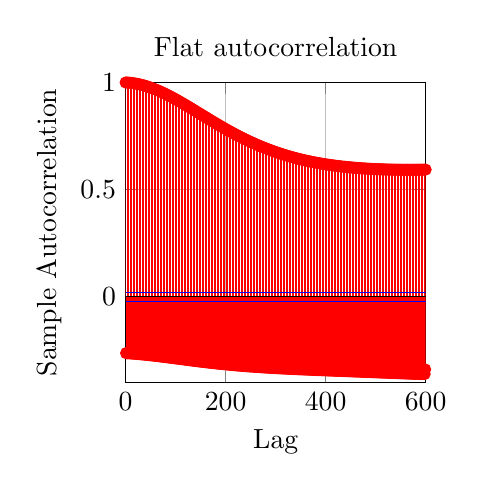
\begin{tikzpicture}

\begin{axis}[%
width=1.5in,
height=1.5in,
scale only axis,
xmin=0,
xmax=600,
xlabel={Lag},
xmajorgrids,
ymin=-0.4,
ymax=1,
ylabel={Sample Autocorrelation},
ymajorgrids,
title={Flat autocorrelation}
]
\addplot[ycomb,color=red,solid,mark size=2.0pt,mark=*,mark options={solid,fill=red}] plot table[row sep=crcr] {%
0	1\\
1	-0.262948449724297\\
2	-0.262463928117916\\
3	0.99962344815621\\
4	-0.263387149800618\\
5	-0.261780902376895\\
6	0.999107331093403\\
7	-0.263851876719128\\
8	-0.261126061603092\\
9	0.998451976493296\\
10	-0.264342134128309\\
11	-0.260499803634412\\
12	0.99765791549299\\
13	-0.26485739428983\\
14	-0.259902493732532\\
15	0.996725881048233\\
16	-0.265397098968693\\
17	-0.259334464284089\\
18	0.99565680563033\\
19	-0.265960660416686\\
20	-0.258796014584992\\
21	0.994451818270657\\
22	-0.266547462447452\\
23	-0.258287410705481\\
24	0.993112240970604\\
25	-0.267156861600905\\
26	-0.257808885433263\\
27	0.991639584498404\\
28	-0.267788188394151\\
29	-0.25736063829184\\
30	0.990035543597835\\
31	-0.268440748655483\\
32	-0.256942835630915\\
33	0.988301991636988\\
34	-0.269113824937429\\
35	-0.256555610785645\\
36	0.98644097472828\\
37	-0.269806678004307\\
38	-0.256199064301366\\
39	0.984454705353603\\
40	-0.270518548389177\\
41	-0.255873264220358\\
42	0.982345555530836\\
43	-0.271248658014576\\
44	-0.255578246427184\\
45	0.980116049560072\\
46	-0.271996211870968\\
47	-0.25531401504913\\
48	0.977768856389573\\
49	-0.27276039974638\\
50	-0.255080542908298\\
51	0.975306781642899\\
52	-0.273540398000343\\
53	-0.254877772021962\\
54	0.972732759349663\\
55	-0.274335371374892\\
56	-0.254705614147886\\
57	0.970049843423083\\
58	-0.275144474835109\\
59	-0.254563951371396\\
60	0.967261198927806\\
61	-0.275966855431495\\
62	-0.254452636731091\\
63	0.964370093181567\\
64	-0.276801654176259\\
65	-0.254371494880256\\
66	0.961379886733865\\
67	-0.277648007925537\\
68	-0.254320322781126\\
69	0.958294024264285\\
70	-0.278505051259527\\
71	-0.25429889042931\\
72	0.95511602544216\\
73	-0.27937191835254\\
74	-0.254306941605844\\
75	0.951849475788114\\
76	-0.28024774482506\\
77	-0.254344194654454\\
78	0.948498017576608\\
79	-0.281131669570095\\
80	-0.254410343281773\\
81	0.94506534081695\\
82	-0.282022836546265\\
83	-0.254505057378377\\
84	0.941555174348428\\
85	-0.282920396530384\\
86	-0.254627983858634\\
87	0.937971277083173\\
88	-0.283823508822613\\
89	-0.25477874751748\\
90	0.934317429428214\\
91	-0.284731342897603\\
92	-0.254956951902335\\
93	0.930597424915927\\
94	-0.285643079995524\\
95	-0.255162180198478\\
96	0.92681506206965\\
97	-0.286557914647261\\
98	-0.255393996126271\\
99	0.922974136528865\\
100	-0.287475056128612\\
101	-0.2556519448487\\
102	0.919078433455789\\
103	-0.288393729838805\\
104	-0.255935553887773\\
105	0.915131720242762\\
106	-0.289313178599197\\
107	-0.256244334048331\\
108	0.911137739537271\\
109	-0.29023266386859\\
110	-0.256577780347911\\
111	0.907100202599001\\
112	-0.291151466872147\\
113	-0.256935372951283\\
114	0.903022783000827\\
115	-0.292068889641476\\
116	-0.257316578108345\\
117	0.898909110683305\\
118	-0.292984255964024\\
119	-0.25772084909403\\
120	0.894762766369887\\
121	-0.293896912240471\\
122	-0.258147627148924\\
123	0.890587276347894\\
124	-0.294806228249393\\
125	-0.258596342419261\\
126	0.886386107618121\\
127	-0.295711597818988\\
128	-0.259066414894973\\
129	0.882162663413976\\
130	-0.29661243940618\\
131	-0.259557255344474\\
132	0.877920279089137\\
133	-0.297508196583912\\
134	-0.260068266244822\\
135	0.873662218370957\\
136	-0.298398338437916\\
137	-0.260598842705919\\
138	0.869391669975208\\
139	-0.299282359874677\\
140	-0.261148373387391\\
141	0.865111744576236\\
142	-0.300159781842718\\
143	-0.261716241406781\\
144	0.860825472125255\\
145	-0.301030151469717\\
146	-0.262301825237701\\
147	0.856535799508243\\
148	-0.301893042118282\\
149	-0.262904499596553\\
150	0.85224558853382\\
151	-0.302748053363531\\
152	-0.263523636316488\\
153	0.847957614240503\\
154	-0.303594810895887\\
155	-0.264158605207229\\
156	0.843674563511903\\
157	-0.30443296635271\\
158	-0.264808774899439\\
159	0.839399033987696\\
160	-0.305262197082586\\
161	-0.26547351367231\\
162	0.83513353325761\\
163	-0.306082205846262\\
164	-0.2661521902631\\
165	0.830880478325184\\
166	-0.306892720458301\\
167	-0.266844174657356\\
168	0.826642195327679\\
169	-0.307693493373649\\
170	-0.26754883885862\\
171	0.822420919498236\\
172	-0.30848430122334\\
173	-0.268265557636452\\
174	0.818218795356224\\
175	-0.309264944303582\\
176	-0.268993709251664\\
177	0.814037877111607\\
178	-0.310035246022483\\
179	-0.269732676157706\\
180	0.809880129269165\\
181	-0.310795052308612\\
182	-0.270481845677218\\
183	0.805747427418478\\
184	-0.311544230985544\\
185	-0.27124061065283\\
186	0.801641559195715\\
187	-0.312282671116472\\
188	-0.272008370071362\\
189	0.797564225403474\\
190	-0.313010282322835\\
191	-0.272784529660647\\
192	0.793517041275175\\
193	-0.313726994080823\\
194	-0.2735685024583\\
195	0.789501537870827\\
196	-0.314432754999463\\
197	-0.274359709351803\\
198	0.785519163591319\\
199	-0.315127532083842\\
200	-0.275157579589406\\
201	0.781571285798803\\
202	-0.315811309986904\\
203	-0.275961551261382\\
204	0.777659192531121\\
205	-0.316484090253007\\
206	-0.276771071751303\\
207	0.773784094298723\\
208	-0.317145890556352\\
209	-0.27758559815705\\
210	0.769947125952942\\
211	-0.317796743937119\\
212	-0.278404597681397\\
213	0.766149348615021\\
214	-0.318436698038044\\
215	-0.279227547992061\\
216	0.76239175165575\\
217	-0.319065814343913\\
218	-0.280053937551198\\
219	0.758675254716131\\
220	-0.31968416742633\\
221	-0.280883265914431\\
222	0.755000709759929\\
223	-0.320291844195865\\
224	-0.28171504399954\\
225	0.751368903149562\\
226	-0.320888943163573\\
227	-0.28254879432504\\
228	0.747780557737241\\
229	-0.321475573713632\\
230	-0.283384051218937\\
231	0.744236334963808\\
232	-0.322051855388731\\
233	-0.284220360998029\\
234	0.740736836958225\\
235	-0.322617917189622\\
236	-0.285057282118166\\
237	0.737282608631148\\
238	-0.323173896890123\\
239	-0.285894385295961\\
240	0.733874139756533\\
241	-0.32371994036869\\
242	-0.286731253602491\\
243	0.730511867035667\\
244	-0.324256200957514\\
245	-0.287567482529574\\
246	0.727196176138504\\
247	-0.324782838809987\\
248	-0.288402680029271\\
249	0.723927403717622\\
250	-0.325300020287223\\
251	-0.289236466527276\\
252	0.72070583939055\\
253	-0.325807917364207\\
254	-0.290068474910933\\
255	0.717531727686633\\
256	-0.326306707056022\\
257	-0.290898350492621\\
258	0.714405269955009\\
259	-0.32679657086451\\
260	-0.291725750949286\\
261	0.711326626230652\\
262	-0.3272776942456\\
263	-0.292550346238942\\
264	0.708295917055794\\
265	-0.327750266097465\\
266	-0.293371818494961\\
267	0.705313225254422\\
268	-0.328214478269575\\
269	-0.294189861899005\\
270	0.702378597657829\\
271	-0.328670525092643\\
272	-0.295004182533465\\
273	0.69949204677957\\
274	-0.329118602929388\\
275	-0.295814498214298\\
276	0.696653552438443\\
277	-0.329558909745984\\
278	-0.296620538305131\\
279	0.693863063328402\\
280	-0.329991644704004\\
281	-0.297422043513554\\
282	0.691120498534607\\
283	-0.330417007772621\\
284	-0.298218765670495\\
285	0.688425748995036\\
286	-0.330835199360807\\
287	-0.299010467493609\\
288	0.685778678907363\\
289	-0.331246419969201\\
290	-0.299796922335577\\
291	0.683179127081\\
292	-0.33165086986132\\
293	-0.300577913918274\\
294	0.680626908234459\\
295	-0.332048748753751\\
296	-0.301353236053714\\
297	0.678121814238354\\
298	-0.332440255524945\\
299	-0.30212269235273\\
300	0.67566361530459\\
301	-0.332825587942217\\
302	-0.302886095922348\\
303	0.673252061122462\\
304	-0.333204942406554\\
305	-0.30364326905279\\
306	0.670886881942542\\
307	-0.333578513714818\\
308	-0.304394042895122\\
309	0.668567789609437\\
310	-0.333946494838933\\
311	-0.305138257130515\\
312	0.666294478544624\\
313	-0.334309076721653\\
314	-0.305875759632137\\
315	0.664066626680743\\
316	-0.334666448088473\\
317	-0.30660640612073\\
318	0.661883896348853\\
319	-0.335018795275313\\
320	-0.307330059814919\\
321	0.659745935120327\\
322	-0.335366302071535\\
323	-0.308046591077366\\
324	0.657652376605142\\
325	-0.335709149577914\\
326	-0.308755877057899\\
327	0.655602841208512\\
328	-0.336047516079166\\
329	-0.309457801334791\\
330	0.653596936847873\\
331	-0.336381576930625\\
332	-0.310152253555427\\
333	0.651634259632381\\
334	-0.336711504458708\\
335	-0.310839129077614\\
336	0.649714394507188\\
337	-0.337037467874746\\
338	-0.311518328612878\\
339	0.647836915864849\\
340	-0.337359633201816\\
341	-0.312189757873143\\
342	0.646001388126334\\
343	-0.337678163214166\\
344	-0.312853327222231\\
345	0.644207366294194\\
346	-0.337993217388821\\
347	-0.313508951333718\\
348	0.64245439648051\\
349	-0.338304951868971\\
350	-0.314156548856724\\
351	0.640742016412352\\
352	-0.338613519438678\\
353	-0.314796042091301\\
354	0.63906975591749\\
355	-0.338919069508462\\
356	-0.315427356675143\\
357	0.637437137393215\\
358	-0.339221748111259\\
359	-0.316050421283406\\
360	0.635843676261095\\
361	-0.339521697908244\\
362	-0.316665167343492\\
363	0.634288881410568\\
364	-0.339819058203917\\
365	-0.31727152876671\\
366	0.632772255634244\\
367	-0.340113964969871\\
368	-0.317869441698758\\
369	0.631293296057787\\
370	-0.340406550876537\\
371	-0.318458844291024\\
372	0.629851494567188\\
373	-0.340696945332182\\
374	-0.319039676494712\\
375	0.628446338236211\\
376	-0.340985274528345\\
377	-0.319611879879798\\
378	0.627077309756647\\
379	-0.341271661490839\\
380	-0.320175397480815\\
381	0.625743887873946\\
382	-0.341556226135339\\
383	-0.32073017367142\\
384	0.624445547830593\\
385	-0.341839085326527\\
386	-0.321276154069606\\
387	0.623181761819435\\
388	-0.342120352939645\\
389	-0.321813285475353\\
390	0.621951999448913\\
391	-0.342400139923242\\
392	-0.322341515842344\\
393	0.620755728221925\\
394	-0.342678554361798\\
395	-0.322860794285228\\
396	0.619592414029704\\
397	-0.342955701536846\\
398	-0.323371071123656\\
399	0.618461521661781\\
400	-0.343231683985102\\
401	-0.323872297964122\\
402	0.61736251533272\\
403	-0.343506601552073\\
404	-0.324364427820276\\
405	0.616294859225903\\
406	-0.343780551439539\\
407	-0.324847415272085\\
408	0.615258018054193\\
409	-0.344053628245266\\
410	-0.325321216663807\\
411	0.614251457636835\\
412	-0.344325923993279\\
413	-0.32578579034032\\
414	0.613274645491464\\
415	-0.344597528153015\\
416	-0.326241096920902\\
417	0.612327051439579\\
418	-0.344868527645714\\
419	-0.326687099609027\\
420	0.611408148223308\\
421	-0.345139006836418\\
422	-0.327123764536251\\
423	0.610517412130807\\
424	-0.345409047510066\\
425	-0.327551061137699\\
426	0.609654323627069\\
427	-0.345678728830249\\
428	-0.327968962556099\\
429	0.608818367986506\\
430	-0.345948127279354\\
431	-0.328377446070779\\
432	0.608009035923141\\
433	-0.346217316578978\\
434	-0.328776493547459\\
435	0.607225824213889\\
436	-0.346486367589749\\
437	-0.329166091904176\\
438	0.606468236310031\\
439	-0.346755348189884\\
440	-0.329546233588165\\
441	0.605735782931693\\
442	-0.347024323132127\\
443	-0.329916917058111\\
444	0.605027982639963\\
445	-0.347293353879022\\
446	-0.330278147265766\\
447	0.604344362381136\\
448	-0.347562498416764\\
449	-0.330629936130676\\
450	0.603684457997573\\
451	-0.347831811048275\\
452	-0.330972303001522\\
453	0.603047814699739\\
454	-0.348101342166476\\
455	-0.331305275097472\\
456	0.602433987494202\\
457	-0.34837113800911\\
458	-0.331628887922955\\
459	0.601842541562634\\
460	-0.348641240396822\\
461	-0.331943185649385\\
462	0.601273052587332\\
463	-0.348911686456576\\
464	-0.332248221457581\\
465	0.600725107019233\\
466	-0.349182508332803\\
467	-0.332544057835012\\
468	0.600198302285056\\
469	-0.349453732888979\\
470	-0.332830766822465\\
471	0.599692246930904\\
472	-0.349725381402589\\
473	-0.333108430205324\\
474	0.59920656070039\\
475	-0.349997469256684\\
476	-0.333377139645349\\
477	0.598740874546268\\
478	-0.350270005631348\\
479	-0.333636996749625\\
480	0.598294830575315\\
481	-0.350542993198543\\
482	-0.333888113074226\\
483	0.597868081927218\\
484	-0.350816427823816\\
485	-0.334130610061044\\
486	0.597460292589015\\
487	-0.351090298278345\\
488	-0.334364618907201\\
489	0.597071137147569\\
490	-0.351364585964688\\
491	-0.334590280367436\\
492	0.596700300483362\\
493	-0.351639264659473\\
494	-0.334807744490819\\
495	0.596347477409661\\
496	-0.351914300276015\\
497	-0.33501717029408\\
498	0.596012372261814\\
499	-0.352189650649605\\
500	-0.335218725374746\\
501	0.595694698442009\\
502	-0.352465265347873\\
503	-0.335412585468057\\
504	0.595394177925332\\
505	-0.352741085508257\\
506	-0.335598933952408\\
507	0.59511054073334\\
508	-0.353017043704226\\
509	-0.335777961308631\\
510	0.594843524381592\\
511	-0.353293063841484\\
512	-0.335949864539003\\
513	0.594592873307741\\
514	-0.353569061084924\\
515	-0.336114846552184\\
516	0.594358338286775\\
517	-0.35384494181671\\
518	-0.3362731155206\\
519	0.594139675839903\\
520	-0.354120603625407\\
521	-0.336424884216879\\
522	0.593936647643339\\
523	-0.354395935325684\\
524	-0.336570369335967\\
525	0.593749019942928\\
526	-0.354670817007761\\
527	-0.33670979080942\\
528	0.593576562980162\\
529	-0.354945120115386\\
530	-0.336843371118148\\
531	0.593419050434625\\
532	-0.355218707550882\\
533	-0.336971334609547\\
534	0.593276258887379\\
535	-0.355491433805515\\
536	-0.337093906824545\\
537	0.593147967309223\\
538	-0.355763145113244\\
539	-0.33721131383959\\
540	0.593033956577135\\
541	-0.356033679625784\\
542	-0.337323781628085\\
543	0.592934009021587\\
544	-0.35630286760677\\
545	-0.337431535445155\\
546	0.59284790800679\\
547	-0.356570531642828\\
548	-0.33753479923906\\
549	0.592775437545332\\
550	-0.356836486869282\\
551	-0.337633795091921\\
552	0.592716381948081\\
553	-0.357100541208355\\
554	-0.337728742691824\\
555	0.592670525509661\\
556	-0.357362495617727\\
557	-0.337819858837769\\
558	0.592637652229327\\
559	-0.357622144347487\\
560	-0.33790735697836\\
561	0.592617545566597\\
562	-0.357879275203655\\
563	-0.337991446784599\\
564	0.592609988230586\\
565	-0.358133669816586\\
566	-0.338072333756655\\
567	0.592614762001654\\
568	-0.358385103912817\\
569	-0.338150218864056\\
570	0.59263164758367\\
571	-0.358633347589062\\
572	-0.338225298218336\\
573	0.592660424484978\\
574	-0.358878165587313\\
575	-0.338297762776887\\
576	0.592700870925946\\
577	-0.359119317570183\\
578	-0.338367798076434\\
579	0.592752763770858\\
580	-0.359356558395855\\
581	-0.33843558399439\\
582	0.592815878481826\\
583	-0.359589638392195\\
584	-0.338501294536151\\
585	0.592889989092351\\
586	-0.35981830362978\\
587	-0.338565097646277\\
588	0.592974868198169\\
589	-0.360042296193763\\
590	-0.33862715504147\\
591	0.59307028696303\\
592	-0.360261354454676\\
593	-0.338687622063196\\
594	0.593176015137156\\
595	-0.360475213338413\\
596	-0.338746647547848\\
597	0.593291821086169\\
598	-0.360683604595762\\
599	-0.338804373712389\\
600	0.593417471828408\\
};
\addplot [color=blue,solid,forget plot]
  table[row sep=crcr]{%
0.5	0.0200010000750062\\
600	0.0200010000750062\\
};
\addplot [color=blue,solid,forget plot]
  table[row sep=crcr]{%
0.5	-0.0200010000750062\\
600	-0.0200010000750062\\
};
\addplot [color=black,solid,forget plot]
  table[row sep=crcr]{%
0	0\\
600	0\\
};
\end{axis}
\end{tikzpicture}%
\end{document}
% This file was created by matlab2tikz.
% Minimal pgfplots version: 1.3
%
%The latest updates can be retrieved from
%  http://www.mathworks.com/matlabcentral/fileexchange/22022-matlab2tikz
%where you can also make suggestions and rate matlab2tikz.
%
\documentclass[tikz]{standalone}
\usepackage{pgfplots}
\usepackage{grffile}
\pgfplotsset{compat=newest}
\usetikzlibrary{plotmarks}
\usepackage{amsmath}

\begin{document}
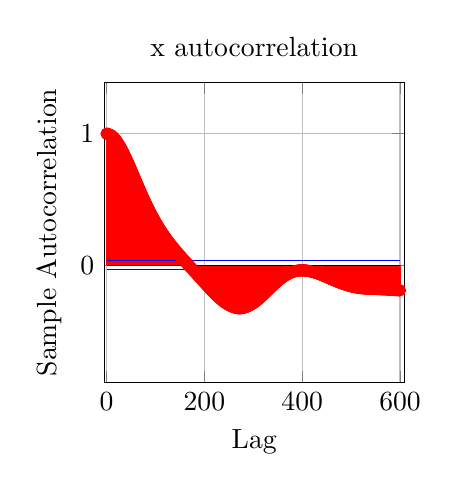
\begin{tikzpicture}

\begin{axis}[%
width=1.5in,
height=1.5in,
scale only axis,
xmin=-4.96357693578217,
xmax=608.389958004124,
xlabel={Lag},
xmajorgrids,
ymin=-0.891386108436905,
ymax=1.3890108309864,
ylabel={Sample Autocorrelation},
ymajorgrids,
title={x autocorrelation}
]
\addplot[ycomb,color=red,solid,mark size=2.0pt,mark=*,mark options={solid,fill=red}] plot table[row sep=crcr] {%
0	1\\
1	0.999688701752999\\
2	0.9991225107778\\
3	0.998301825462279\\
4	0.997227315792302\\
5	0.9958999217757\\
6	0.994320851238136\\
7	0.992491576999675\\
8	0.990413833443373\\
9	0.9880896124897\\
10	0.985521158992928\\
11	0.982710965577927\\
12	0.97966176693789\\
13	0.976376533615569\\
14	0.972858465292423\\
15	0.969110983611797\\
16	0.965137724563812\\
17	0.960942530460975\\
18	0.956529441534759\\
19	0.951902687184399\\
20	0.947066676909977\\
21	0.942025990962547\\
22	0.9367853707445\\
23	0.931349708993674\\
24	0.925724039784813\\
25	0.919913528381946\\
26	0.913923460975015\\
27	0.907759234333702\\
28	0.901426345410876\\
29	0.894930380927404\\
30	0.888277006969258\\
31	0.881471958626924\\
32	0.874521029706057\\
33	0.867430062537202\\
34	0.860204937911137\\
35	0.8528515651651\\
36	0.845375872443754\\
37	0.837783797157298\\
38	0.83008127665767\\
39	0.822274239152211\\
40	0.814368594872654\\
41	0.806370227515694\\
42	0.798284985969837\\
43	0.790118676341662\\
44	0.781877054293043\\
45	0.773565817699349\\
46	0.765190599637137\\
47	0.756756961708349\\
48	0.748270387706582\\
49	0.739736277629627\\
50	0.731159942041093\\
51	0.72254659678266\\
52	0.713901358037253\\
53	0.705229237742273\\
54	0.696535139350883\\
55	0.687823853938326\\
56	0.67910005664925\\
57	0.670368303481122\\
58	0.661633028397951\\
59	0.652898540767772\\
60	0.644169023116651\\
61	0.635448529191283\\
62	0.62674098232175\\
63	0.618050174075427\\
64	0.609379763192626\\
65	0.600733274794167\\
66	0.592114099850729\\
67	0.583525494903589\\
68	0.574970582026123\\
69	0.566452349015297\\
70	0.557973649802257\\
71	0.549537205071063\\
72	0.5411456030746\\
73	0.532801300636711\\
74	0.524506624329671\\
75	0.516263771816202\\
76	0.508074813345371\\
77	0.499941693391872\\
78	0.491866232428377\\
79	0.483850128820869\\
80	0.475894960837073\\
81	0.468002188758414\\
82	0.460173157086142\\
83	0.45240909683261\\
84	0.444711127888957\\
85	0.437080261460788\\
86	0.429517402563748\\
87	0.422023352571242\\
88	0.414598811806864\\
89	0.407244382174473\\
90	0.399960569819161\\
91	0.392747787812746\\
92	0.385606358857728\\
93	0.378536518004023\\
94	0.37153841537311\\
95	0.364612118884577\\
96	0.357757616980381\\
97	0.350974821342458\\
98	0.344263569599658\\
99	0.337623628020264\\
100	0.331054694186708\\
101	0.324556399649328\\
102	0.31812831255637\\
103	0.311769940257668\\
104	0.305480731879713\\
105	0.299260080870105\\
106	0.293107327509594\\
107	0.287021761390183\\
108	0.281002623857956\\
109	0.27504911041955\\
110	0.269160373111346\\
111	0.263335522830658\\
112	0.257573631628394\\
113	0.251873734962776\\
114	0.246234833913896\\
115	0.240655897358998\\
116	0.235135864108487\\
117	0.229673645002799\\
118	0.224268124970318\\
119	0.218918165046631\\
120	0.213622604355464\\
121	0.208380262051685\\
122	0.203189939226792\\
123	0.198050420777329\\
124	0.192960477236672\\
125	0.187918866570621\\
126	0.182924335937207\\
127	0.177975623411093\\
128	0.173071459672908\\
129	0.168210569663792\\
130	0.163391674205353\\
131	0.158613491585207\\
132	0.153874739108147\\
133	0.149174134612935\\
134	0.144510397954632\\
135	0.139882252452275\\
136	0.135288426301673\\
137	0.130727653952966\\
138	0.126198677452593\\
139	0.121700247749198\\
140	0.117231125963013\\
141	0.112790084618211\\
142	0.108375908837708\\
143	0.103987397499942\\
144	0.0996233643571561\\
145	0.0952826391148032\\
146	0.0909640684717697\\
147	0.0866665171212173\\
148	0.0823888687119961\\
149	0.0781300267707302\\
150	0.0738889155848704\\
151	0.0696644810472078\\
152	0.0654556914625639\\
153	0.0612615383176128\\
154	0.057081037015028\\
155	0.0529132275734023\\
156	0.048757175294631\\
157	0.0446119714006944\\
158	0.0404767336419988\\
159	0.0363506068796511\\
160	0.0322327636442239\\
161	0.0281224046737271\\
162	0.0240187594336236\\
163	0.0199210866218135\\
164	0.0158286746615522\\
165	0.0117408421852681\\
166	0.00765693851219828\\
167	0.00357634412266923\\
168	-0.000501528868287381\\
169	-0.00457723623547877\\
170	-0.00865130116396778\\
171	-0.0127242137633375\\
172	-0.0167964305740729\\
173	-0.0208683740646482\\
174	-0.024940432118255\\
175	-0.0290129575084677\\
176	-0.0330862673635145\\
177	-0.0371606426192038\\
178	-0.0412363274609301\\
179	-0.0453135287555607\\
180	-0.0493924154743612\\
181	-0.0534731181084688\\
182	-0.0575557280787472\\
183	-0.0616402971421606\\
184	-0.0657268367970868\\
185	-0.0698153176902369\\
186	-0.0739056690280794\\
187	-0.0779977779958517\\
188	-0.0820914891874141\\
189	-0.0861866040493331\\
190	-0.090282880342688\\
191	-0.0943800316261736\\
192	-0.0984777267641261\\
193	-0.102575589463127\\
194	-0.106673197840847\\
195	-0.110770084030771\\
196	-0.114865733826421\\
197	-0.118959586368639\\
198	-0.123051033879411\\
199	-0.127139421445654\\
200	-0.13122404685629\\
201	-0.135304160495797\\
202	-0.139378965297369\\
203	-0.143447616758632\\
204	-0.147509223022787\\
205	-0.15156284502787\\
206	-0.155607496726702\\
207	-0.159642145379941\\
208	-0.163665711924501\\
209	-0.167677071419421\\
210	-0.171675053571127\\
211	-0.175658443339847\\
212	-0.17962598162875\\
213	-0.183576366057231\\
214	-0.187508251819529\\
215	-0.191420252629735\\
216	-0.195310941753985\\
217	-0.199178853130483\\
218	-0.203022482577764\\
219	-0.2068402890914\\
220	-0.210630696229133\\
221	-0.214392093584217\\
222	-0.218122838346478\\
223	-0.221821256950427\\
224	-0.225485646809475\\
225	-0.229114278135093\\
226	-0.232705395839498\\
227	-0.236257221520221\\
228	-0.239767955524622\\
229	-0.243235779092246\\
230	-0.24665885657256\\
231	-0.250035337715468\\
232	-0.253363360031666\\
233	-0.256641051219697\\
234	-0.25986653165632\\
235	-0.263037916946536\\
236	-0.266153320529409\\
237	-0.269210856335574\\
238	-0.272208641492096\\
239	-0.275144799070132\\
240	-0.278017460870632\\
241	-0.280824770243133\\
242	-0.28356488493248\\
243	-0.286235979948161\\
244	-0.288836250450764\\
245	-0.291363914649901\\
246	-0.293817216707836\\
247	-0.296194429642903\\
248	-0.298493858226707\\
249	-0.300713841869021\\
250	-0.302852757484187\\
251	-0.304909022332825\\
252	-0.306881096832569\\
253	-0.308767487331567\\
254	-0.310566748838472\\
255	-0.312277487702673\\
256	-0.313898364238564\\
257	-0.315428095287708\\
258	-0.316865456712841\\
259	-0.318209285817762\\
260	-0.319458483687274\\
261	-0.320612017441502\\
262	-0.321668922399066\\
263	-0.322628304143753\\
264	-0.323489340489587\\
265	-0.324251283339348\\
266	-0.324913460431892\\
267	-0.325475276973839\\
268	-0.325936217151478\\
269	-0.326295845519049\\
270	-0.326553808259828\\
271	-0.326709834316776\\
272	-0.326763736389862\\
273	-0.326715411797464\\
274	-0.32656484319965\\
275	-0.326312099181477\\
276	-0.325957334694819\\
277	-0.325500791357615\\
278	-0.32494279760981\\
279	-0.324283768725647\\
280	-0.323524206682341\\
281	-0.322664699885592\\
282	-0.321705922752737\\
283	-0.320648635154774\\
284	-0.319493681718831\\
285	-0.318241990993072\\
286	-0.316894574476376\\
287	-0.315452525515503\\
288	-0.313917018072814\\
289	-0.312289305367951\\
290	-0.310570718397228\\
291	-0.308762664334769\\
292	-0.306866624819783\\
293	-0.304884154134591\\
294	-0.302816877278332\\
295	-0.3006664879415\\
296	-0.298434746386688\\
297	-0.296123477241141\\
298	-0.293734567206862\\
299	-0.291269962694224\\
300	-0.288731667385118\\
301	-0.286121739731826\\
302	-0.283442290397859\\
303	-0.28069547964706\\
304	-0.277883514687318\\
305	-0.27500864697523\\
306	-0.272073169488031\\
307	-0.269079413969055\\
308	-0.266029748152944\\
309	-0.262926572976688\\
310	-0.259772319782487\\
311	-0.256569447518266\\
312	-0.253320439941514\\
313	-0.25002780283192\\
314	-0.246694061218095\\
315	-0.24332175662341\\
316	-0.239913444335766\\
317	-0.236471690705849\\
318	-0.23299907047814\\
319	-0.229498164158679\\
320	-0.225971555423306\\
321	-0.222421828569769\\
322	-0.218851566016825\\
323	-0.21526334585312\\
324	-0.211659739438364\\
325	-0.208043309058964\\
326	-0.204416605640032\\
327	-0.200782166515325\\
328	-0.197142513256445\\
329	-0.193500149562289\\
330	-0.18985755920951\\
331	-0.186217204064469\\
332	-0.18258152215691\\
333	-0.178952925815384\\
334	-0.175333799864199\\
335	-0.17172649988151\\
336	-0.168133350517962\\
337	-0.164556643875165\\
338	-0.160998637943106\\
339	-0.157461555095536\\
340	-0.153947580642226\\
341	-0.150458861436942\\
342	-0.146997504539923\\
343	-0.143565575933614\\
344	-0.140165099290399\\
345	-0.136798054791067\\
346	-0.133466377992807\\
347	-0.130171958745513\\
348	-0.126916640155312\\
349	-0.123702217594235\\
350	-0.120530437755085\\
351	-0.117402997750647\\
352	-0.114321544256488\\
353	-0.111287672696729\\
354	-0.108302926472304\\
355	-0.105368796231345\\
356	-0.102486719181474\\
357	-0.0996580784439451\\
358	-0.0968842024496938\\
359	-0.0941663643775086\\
360	-0.0915057816346746\\
361	-0.0889036153805666\\
362	-0.0863609700937989\\
363	-0.0838788931836496\\
364	-0.0814583746465909\\
365	-0.0791003467688413\\
366	-0.0768056838759467\\
367	-0.0745752021304568\\
368	-0.0724096593788219\\
369	-0.0703097550486641\\
370	-0.0682761300976056\\
371	-0.0663093670148288\\
372	-0.0644099898765382\\
373	-0.0625784644564534\\
374	-0.0608151983924165\\
375	-0.0591205414101296\\
376	-0.0574947856049515\\
377	-0.0559381657825853\\
378	-0.0544508598593671\\
379	-0.0530329893227408\\
380	-0.051684619752354\\
381	-0.050405761402054\\
382	-0.0491963698428954\\
383	-0.0480563466670868\\
384	-0.0469855402526216\\
385	-0.0459837465881395\\
386	-0.0450507101573629\\
387	-0.0441861248822509\\
388	-0.043389635123804\\
389	-0.0426608367392409\\
390	-0.0419992781940649\\
391	-0.0414044617273258\\
392	-0.0408758445681838\\
393	-0.0404128402016779\\
394	-0.0400148196814108\\
395	-0.0396811129866752\\
396	-0.0394110104213658\\
397	-0.0392037640518531\\
398	-0.0390585891808316\\
399	-0.0389746658540091\\
400	-0.0389511403963594\\
401	-0.0389871269745371\\
402	-0.0390817091819328\\
403	-0.0392339416427467\\
404	-0.0394428516313665\\
405	-0.0397074407032513\\
406	-0.0400266863334663\\
407	-0.0403995435589515\\
408	-0.0408249466205721\\
409	-0.0413018106009708\\
410	-0.0418290330542275\\
411	-0.0424054956233353\\
412	-0.0430300656415132\\
413	-0.0437015977134079\\
414	-0.0444189352722778\\
415	-0.0451809121093166\\
416	-0.045986353871343\\
417	-0.0468340795231813\\
418	-0.0477229027711607\\
419	-0.0486516334442954\\
420	-0.0496190788298472\\
421	-0.0506240449601391\\
422	-0.0516653378476788\\
423	-0.0527417646658457\\
424	-0.0538521348726318\\
425	-0.0549952612751646\\
426	-0.056169961033011\\
427	-0.0573750565985439\\
428	-0.0586093765929615\\
429	-0.0598717566168635\\
430	-0.061161039994635\\
431	-0.0624760784522276\\
432	-0.0638157327282989\\
433	-0.0651788731190294\\
434	-0.0665643799573128\\
435	-0.0679711440273894\\
436	-0.0693980669163538\\
437	-0.070844061304336\\
438	-0.0723080511954964\\
439	-0.0737889720923124\\
440	-0.07528577111594\\
441	-0.0767974070757248\\
442	-0.0783228504911909\\
443	-0.0798610835700671\\
444	-0.0814111001461011\\
445	-0.082971905580572\\
446	-0.0845425166315325\\
447	-0.0861219612948963\\
448	-0.0877092786215364\\
449	-0.0893035185145698\\
450	-0.0909037415109843\\
451	-0.0925090185517113\\
452	-0.094118430744166\\
453	-0.0957310691211726\\
454	-0.0973460344000681\\
455	-0.0989624367456314\\
456	-0.10057939554034\\
457	-0.102196039165289\\
458	-0.103811504794938\\
459	-0.105424938208721\\
460	-0.107035493622348\\
461	-0.108642333541532\\
462	-0.110244628640703\\
463	-0.111841557669172\\
464	-0.113432307387101\\
465	-0.11501607253354\\
466	-0.116592055828733\\
467	-0.118159468012859\\
468	-0.119717527923306\\
469	-0.121265462612605\\
470	-0.122802507509122\\
471	-0.124327906622607\\
472	-0.12584091279675\\
473	-0.127340788010881\\
474	-0.128826803732968\\
475	-0.130298241326107\\
476	-0.131754392510665\\
477	-0.133194559884217\\
478	-0.134618057501402\\
479	-0.136024211515688\\
480	-0.137412360884969\\
481	-0.138781858142711\\
482	-0.140132070236154\\
483	-0.141462379432774\\
484	-0.142772184295872\\
485	-0.144060900729675\\
486	-0.145327963093852\\
487	-0.146572825386682\\
488	-0.147794962495421\\
489	-0.148993871511565\\
490	-0.150169073107804\\
491	-0.151320112972378\\
492	-0.152446563295457\\
493	-0.153548024300868\\
494	-0.154624125815187\\
495	-0.15567452886478\\
496	-0.156698927289893\\
497	-0.157697049363352\\
498	-0.158668659399896\\
499	-0.159613559340613\\
500	-0.160531590295445\\
501	-0.161422634025353\\
502	-0.162286614344408\\
503	-0.163123498421023\\
504	-0.163933297956631\\
505	-0.164716070219579\\
506	-0.165471918911724\\
507	-0.16620099484539\\
508	-0.166903496408912\\
509	-0.167579669800062\\
510	-0.16822980900819\\
511	-0.168854255528041\\
512	-0.169453397790768\\
513	-0.170027670300854\\
514	-0.170577552471241\\
515	-0.171103567153024\\
516	-0.171606278860541\\
517	-0.172086291697354\\
518	-0.172544246993575\\
519	-0.172980820669906\\
520	-0.173396720348717\\
521	-0.173792682237132\\
522	-0.174169467811522\\
523	-0.174527860336636\\
524	-0.174868661255963\\
525	-0.175192686492467\\
526	-0.175500762700708\\
527	-0.175793723512256\\
528	-0.17607240581644\\
529	-0.176337646117602\\
530	-0.176590277008355\\
531	-0.176831123795817\\
532	-0.177061001314544\\
533	-0.177280710955962\\
534	-0.177491037939704\\
535	-0.177692748847434\\
536	-0.177886589434685\\
537	-0.178073282731059\\
538	-0.178253527434041\\
539	-0.178427996596639\\
540	-0.178597336604424\\
541	-0.17876216643316\\
542	-0.178923077174356\\
543	-0.179080631812706\\
544	-0.179235365236545\\
545	-0.179387784460213\\
546	-0.179538369035548\\
547	-0.179687571628591\\
548	-0.17983581873701\\
549	-0.179983511523651\\
550	-0.18013102674195\\
551	-0.180278717729683\\
552	-0.180426915448581\\
553	-0.180575929548658\\
554	-0.180726049437652\\
555	-0.180877545337689\\
556	-0.181030669313045\\
557	-0.181185656254806\\
558	-0.18134272481007\\
559	-0.181502078245231\\
560	-0.181663905234684\\
561	-0.181828380568086\\
562	-0.18199566577091\\
563	-0.182165909634661\\
564	-0.182339248654492\\
565	-0.182515807373341\\
566	-0.182695698632879\\
567	-0.182879023732628\\
568	-0.183065872499597\\
569	-0.18325632327158\\
570	-0.183450442798006\\
571	-0.183648286062856\\
572	-0.183849896034662\\
573	-0.184055303349052\\
574	-0.184264525929645\\
575	-0.184477568553373\\
576	-0.184694422366501\\
577	-0.184915064357778\\
578	-0.185139456795226\\
579	-0.18536754663312\\
580	-0.185599264895695\\
581	-0.185834526044119\\
582	-0.186073227333136\\
583	-0.186315248163752\\
584	-0.186560449438155\\
585	-0.186808672922953\\
586	-0.187059740626639\\
587	-0.187313454196999\\
588	-0.187569594344017\\
589	-0.187827920293592\\
590	-0.188088169277185\\
591	-0.188350056062296\\
592	-0.188613272528404\\
593	-0.188877487292811\\
594	-0.189142345390532\\
595	-0.189407468012153\\
596	-0.189672452303298\\
597	-0.189936871229094\\
598	-0.19020027350673\\
599	-0.190462183608947\\
600	-0.190722101840988\\
};
\addplot [color=blue,solid,forget plot]
  table[row sep=crcr]{%
0.5	0.0346427483320998\\
600	0.0346427483320998\\
};
\addplot [color=blue,solid,forget plot]
  table[row sep=crcr]{%
0.5	-0.0346427483320998\\
600	-0.0346427483320998\\
};
\addplot [color=black,solid,forget plot]
  table[row sep=crcr]{%
0	0\\
600	0\\
};
\end{axis}
\end{tikzpicture}%
\end{document}
% This file was created by matlab2tikz.
% Minimal pgfplots version: 1.3
%
%The latest updates can be retrieved from
%  http://www.mathworks.com/matlabcentral/fileexchange/22022-matlab2tikz
%where you can also make suggestions and rate matlab2tikz.
%
\documentclass[tikz]{standalone}
\usepackage{pgfplots}
\usepackage{grffile}
\pgfplotsset{compat=newest}
\usetikzlibrary{plotmarks}
\usepackage{amsmath}

\begin{document}
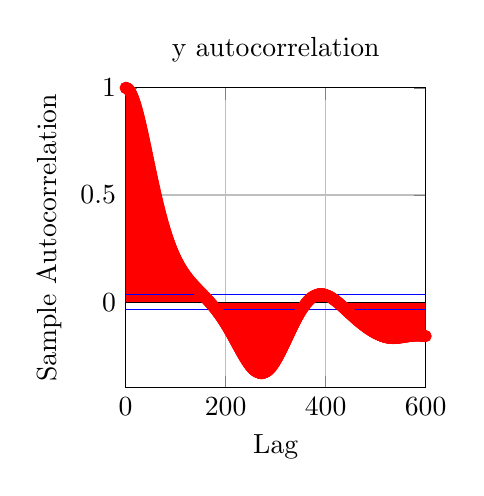
\begin{tikzpicture}

\begin{axis}[%
width=1.5in,
height=1.5in,
scale only axis,
xmin=0,
xmax=600,
xlabel={Lag},
xmajorgrids,
ymin=-0.4,
ymax=1,
ylabel={Sample Autocorrelation},
ymajorgrids,
title={y autocorrelation}
]
\addplot[ycomb,color=red,solid,mark size=2.0pt,mark=*,mark options={solid,fill=red}] plot table[row sep=crcr] {%
0	1\\
1	0.999731024526725\\
2	0.999032892866843\\
3	0.997906698426239\\
4	0.996354284977762\\
5	0.994378239826315\\
6	0.991981884264389\\
7	0.989169261378612\\
8	0.985945121284201\\
9	0.982314903879785\\
10	0.978284719229761\\
11	0.97386132569498\\
12	0.969052105945096\\
13	0.963865040997145\\
14	0.958308682434859\\
15	0.952392122971751\\
16	0.946124965528045\\
17	0.939517290997147\\
18	0.932579624881407\\
19	0.925322902979531\\
20	0.917758436309091\\
21	0.909897875447299\\
22	0.901753174471454\\
23	0.89333655467749\\
24	0.884660468250753\\
25	0.87573756205773\\
26	0.866580641720982\\
27	0.857202636132098\\
28	0.847616562549247\\
29	0.837835492416885\\
30	0.827872518035615\\
31	0.817740720200086\\
32	0.807453136912359\\
33	0.797022733267441\\
34	0.786462372596795\\
35	0.775784788944704\\
36	0.76500256094146\\
37	0.754128087126614\\
38	0.743173562764962\\
39	0.732150958187718\\
40	0.721071998681434\\
41	0.709948145937791\\
42	0.698790581068363\\
43	0.687610189180043\\
44	0.676417545498826\\
45	0.665222903022374\\
46	0.654036181674968\\
47	0.64286695893234\\
48	0.631724461878314\\
49	0.620617560650255\\
50	0.609554763225987\\
51	0.598544211501073\\
52	0.587593678602193\\
53	0.576710567379692\\
54	0.565901910020292\\
55	0.555174368719324\\
56	0.544534237350731\\
57	0.533987444072368\\
58	0.523539554803862\\
59	0.513195777514383\\
60	0.502960967258101\\
61	0.4928396318959\\
62	0.48283593844291\\
63	0.472953719982739\\
64	0.463196483090801\\
65	0.45356741571082\\
66	0.444069395430488\\
67	0.434704998104241\\
68	0.425476506773263\\
69	0.41638592083503\\
70	0.407434965416991\\
71	0.39862510091133\\
72	0.389957532630097\\
73	0.381433220542396\\
74	0.373052889057673\\
75	0.364817036821524\\
76	0.356725946492778\\
77	0.348779694472877\\
78	0.340978160560864\\
79	0.333321037509455\\
80	0.325807840459782\\
81	0.318437916234501\\
82	0.311210452470894\\
83	0.304124486577523\\
84	0.297178914499815\\
85	0.290372499281702\\
86	0.283703879412082\\
87	0.277171576946455\\
88	0.270774005395561\\
89	0.264509477374255\\
90	0.258376212005158\\
91	0.252372342072859\\
92	0.246495920925597\\
93	0.240744929122415\\
94	0.235117280824751\\
95	0.229610829932386\\
96	0.224223375964468\\
97	0.218952669687107\\
98	0.213796418489772\\
99	0.208752291513301\\
100	0.203817924532948\\
101	0.198990924600388\\
102	0.194268874449053\\
103	0.189649336667574\\
104	0.185129857646459\\
105	0.180707971303426\\
106	0.176381202593067\\
107	0.172147070806729\\
108	0.16800309266867\\
109	0.163946785234666\\
110	0.159975668599353\\
111	0.156087268418639\\
112	0.15227911825355\\
113	0.148548761741887\\
114	0.144893754604022\\
115	0.141311666489141\\
116	0.137800082668139\\
117	0.134356605579313\\
118	0.130978856232866\\
119	0.127664475480131\\
120	0.124411125153287\\
121	0.121216489081188\\
122	0.118078273986795\\
123	0.114994210271542\\
124	0.111962052691806\\
125	0.108979580932525\\
126	0.106044600082837\\
127	0.103154941018512\\
128	0.100308460695789\\
129	0.097503042361157\\
130	0.0947365956815132\\
131	0.0920070567990681\\
132	0.0893123883153283\\
133	0.0866505792084686\\
134	0.0840196446884246\\
135	0.0814176259940791\\
136	0.0788425901369945\\
137	0.0762926295962568\\
138	0.0737658619691408\\
139	0.0712604295824803\\
140	0.0687744990698382\\
141	0.0663062609198015\\
142	0.0638539290009847\\
143	0.061415740069598\\
144	0.0589899532657237\\
145	0.0565748496047306\\
146	0.054168731470544\\
147	0.0517699221177565\\
148	0.0493767651898115\\
149	0.0469876242607068\\
150	0.044600882407829\\
151	0.042214941823647\\
152	0.0398282234740405\\
153	0.0374391668110131\\
154	0.0350462295474421\\
155	0.0326478875013193\\
156	0.0302426345166634\\
157	0.02782898246791\\
158	0.0254054613541236\\
159	0.0229706194888273\\
160	0.0205230237906116\\
161	0.0180612601789809\\
162	0.0155839340791229\\
163	0.0130896710384687\\
164	0.0105771174570502\\
165	0.00804494143277858\\
166	0.00549183372188004\\
167	0.00291650881384199\\
168	0.000317706119365553\\
169	-0.00230580873100232\\
170	-0.00495524248064997\\
171	-0.00763177273690282\\
172	-0.0103365463616842\\
173	-0.0130706777678408\\
174	-0.0158352471266112\\
175	-0.0186312984921175\\
176	-0.0214598378490676\\
177	-0.0243218310900962\\
178	-0.0272182019293256\\
179	-0.0301498297588252\\
180	-0.0331175474546805\\
181	-0.0361221391393646\\
182	-0.039164337907054\\
183	-0.0422448235184419\\
184	-0.0453642200715009\\
185	-0.0485230936545376\\
186	-0.051721949987764\\
187	-0.0549612320595146\\
188	-0.0582413177631468\\
189	-0.0615625175406004\\
190	-0.0649250720385535\\
191	-0.0683291497831047\\
192	-0.0717748448789386\\
193	-0.0752621747389891\\
194	-0.0787910778507074\\
195	-0.0823614115851672\\
196	-0.0859729500553915\\
197	-0.089625382030466\\
198	-0.093318308912208\\
199	-0.0970512427813787\\
200	-0.100823604520663\\
201	-0.104634722021881\\
202	-0.108483828485144\\
203	-0.112370060817904\\
204	-0.116292458142086\\
205	-0.120249960417714\\
206	-0.124241407191631\\
207	-0.128265536480099\\
208	-0.132320983794217\\
209	-0.136406281317194\\
210	-0.140519857242593\\
211	-0.144660035282706\\
212	-0.148825034356176\\
213	-0.153012968463951\\
214	-0.157221846762504\\
215	-0.161449573843094\\
216	-0.165693950225618\\
217	-0.169952673075275\\
218	-0.174223337149955\\
219	-0.178503435985803\\
220	-0.182790363327953\\
221	-0.18708141481287\\
222	-0.191373789908138\\
223	-0.195664594114829\\
224	-0.199950841436911\\
225	-0.204229457121296\\
226	-0.208497280671323\\
227	-0.21275106913555\\
228	-0.216987500672769\\
229	-0.221203178393155\\
230	-0.225394634474422\\
231	-0.229558334550757\\
232	-0.233690682371188\\
233	-0.237788024722896\\
234	-0.241846656613807\\
235	-0.245862826707604\\
236	-0.249832743003113\\
237	-0.253752578748811\\
238	-0.257618478582001\\
239	-0.261426564881028\\
240	-0.265172944317715\\
241	-0.268853714596108\\
242	-0.272464971362444\\
243	-0.276002815270247\\
244	-0.279463359183414\\
245	-0.282842735499183\\
246	-0.286137103571981\\
247	-0.289342657218335\\
248	-0.292455632282221\\
249	-0.295472314239605\\
250	-0.298389045820288\\
251	-0.301202234624694\\
252	-0.303908360712806\\
253	-0.306503984142169\\
254	-0.308985752431631\\
255	-0.31135040792742\\
256	-0.313594795048119\\
257	-0.315715867385223\\
258	-0.317710694636143\\
259	-0.319576469346854\\
260	-0.32131051344178\\
261	-0.322910284519039\\
262	-0.324373381889766\\
263	-0.325697552340965\\
264	-0.326880695602137\\
265	-0.327920869496824\\
266	-0.328816294761202\\
267	-0.329565359512908\\
268	-0.330166623354432\\
269	-0.330618821096619\\
270	-0.330920866089089\\
271	-0.33107185314575\\
272	-0.331071061054924\\
273	-0.330917954665106\\
274	-0.330612186538794\\
275	-0.330153598168414\\
276	-0.329542220749852\\
277	-0.328778275510736\\
278	-0.327862173592161\\
279	-0.326794515484177\\
280	-0.325576090016979\\
281	-0.324207872911322\\
282	-0.322691024893333\\
283	-0.321026889380432\\
284	-0.31921698974671\\
285	-0.3172630261776\\
286	-0.315166872125262\\
287	-0.312930570377527\\
288	-0.310556328754715\\
289	-0.30804651545004\\
290	-0.305403654030599\\
291	-0.302630418117278\\
292	-0.299729625763031\\
293	-0.296704233550178\\
294	-0.293557330428342\\
295	-0.290292131315648\\
296	-0.286911970486607\\
297	-0.283420294770898\\
298	-0.279820656587866\\
299	-0.2761167068421\\
300	-0.272312187705852\\
301	-0.268410925314342\\
302	-0.264416822400135\\
303	-0.260333850892826\\
304	-0.256166044510114\\
305	-0.251917491366138\\
306	-0.247592326622527\\
307	-0.24319472520711\\
308	-0.23872889462457\\
309	-0.234199067882511\\
310	-0.229609496555502\\
311	-0.224964444008583\\
312	-0.220268178800555\\
313	-0.215524968286066\\
314	-0.210739072434109\\
315	-0.205914737879029\\
316	-0.201056192218548\\
317	-0.196167638571636\\
318	-0.191253250407299\\
319	-0.186317166653541\\
320	-0.181363487093936\\
321	-0.176396268057308\\
322	-0.171419518404167\\
323	-0.166437195811594\\
324	-0.161453203356407\\
325	-0.156471386394539\\
326	-0.151495529732736\\
327	-0.14652935508691\\
328	-0.141576518819738\\
329	-0.136640609948501\\
330	-0.131725148412582\\
331	-0.126833583588637\\
332	-0.121969293040102\\
333	-0.117135581486542\\
334	-0.112335679977267\\
335	-0.10757274525275\\
336	-0.102849859276613\\
337	-0.0981700289203598\\
338	-0.0935361857826017\\
339	-0.08895118612424\\
340	-0.0844178109009929\\
341	-0.0799387658747068\\
342	-0.0755166817851366\\
343	-0.0711541145642848\\
344	-0.0668535455759478\\
345	-0.0626173818638437\\
346	-0.0584479563925611\\
347	-0.0543475282665803\\
348	-0.0503182829137608\\
349	-0.0463623322209488\\
350	-0.0424817146107325\\
351	-0.0386783950498396\\
352	-0.0349542649812201\\
353	-0.0313111421734755\\
354	-0.0277507704829655\\
355	-0.0242748195256266\\
356	-0.0208848842572638\\
357	-0.0175824844628022\\
358	-0.0143690641567014\\
359	-0.0112459908984155\\
360	-0.00821455502841716\\
361	-0.00527596883187605\\
362	-0.00243136563857179\\
363	0.000318201130985484\\
364	0.00297175896196056\\
365	0.00552841727170251\\
366	0.00798736845290125\\
367	0.0103478889190537\\
368	0.012609340137171\\
369	0.0147711696320959\\
370	0.0168329119463959\\
371	0.0187941895395794\\
372	0.0206547136103285\\
373	0.02241428482557\\
374	0.0240727939405092\\
375	0.0256302222942242\\
376	0.027086642166056\\
377	0.0284422169788366\\
378	0.02969720133594\\
379	0.0308519408802446\\
380	0.0319068719643091\\
381	0.0328625211224115\\
382	0.0337195043365384\\
383	0.0344785260899447\\
384	0.0351403782035012\\
385	0.0357059384517092\\
386	0.0361761689569465\\
387	0.0365521143622285\\
388	0.0368348997844788\\
389	0.0370257285520071\\
390	0.03712587973156\\
391	0.037136705451929\\
392	0.0370596280326629\\
393	0.0368961369279072\\
394	0.0366477854967814\\
395	0.0363161876129966\\
396	0.0359030141275778\\
397	0.0354099891996085\\
398	0.03483888651083\\
399	0.034191525380704\\
400	0.0334697667991802\\
401	0.0326755093949032\\
402	0.0318106853569288\\
403	0.0308772563282146\\
404	0.0298772092891915\\
405	0.0288125524496251\\
406	0.0276853111667343\\
407	0.0264975239071526\\
408	0.0252512382698144\\
409	0.0239485070862149\\
410	0.0225913846137415\\
411	0.0211819228369235\\
412	0.0197221678904894\\
413	0.0182141566170798\\
414	0.016659913271342\\
415	0.0150614463809399\\
416	0.0134207457737673\\
417	0.011739779779356\\
418	0.0100204926111404\\
419	0.00826480193488455\\
420	0.00647459662721319\\
421	0.00465173472681859\\
422	0.0027980415795593\\
423	0.000915308177334009\\
424	-0.00099471031068613\\
425	-0.00293029581713194\\
426	-0.00488976846968368\\
427	-0.00687148750347165\\
428	-0.00887385199866486\\
429	-0.0108953014502277\\
430	-0.0129343161776817\\
431	-0.0149894175834529\\
432	-0.0170591682690118\\
433	-0.0191421720185156\\
434	-0.0212370736600464\\
435	-0.0233425588147736\\
436	-0.0254573535444945\\
437	-0.0275802239079817\\
438	-0.0297099754364248\\
439	-0.0318454525379831\\
440	-0.0339855378410814\\
441	-0.0361291514855873\\
442	-0.0382752503704197\\
443	-0.0404228273654629\\
444	-0.0425709104949197\\
445	-0.044718562098433\\
446	-0.0468648779754697\\
447	-0.0490089865175971\\
448	-0.0511500478324111\\
449	-0.0532872528620104\\
450	-0.0554198224980766\\
451	-0.0575470066948078\\
452	-0.0596680835802075\\
453	-0.0617823585655239\\
454	-0.0638891634520156\\
455	-0.0659878555336614\\
456	-0.0680778166939609\\
457	-0.0701584524945819\\
458	-0.0722291912533116\\
459	-0.0742894831085409\\
460	-0.0763387990673871\\
461	-0.0783766300344966\\
462	-0.0804024858186007\\
463	-0.0824158941139907\\
464	-0.0844163994542503\\
465	-0.0864035621358098\\
466	-0.0883769571091867\\
467	-0.0903361728361178\\
468	-0.0922808101111989\\
469	-0.094210480847091\\
470	-0.0961248068228581\\
471	-0.0980234183955429\\
472	-0.0999059531756784\\
473	-0.10177205466807\\
474	-0.103621370879862\\
475	-0.105453552898638\\
476	-0.107268253444076\\
477	-0.109065125397507\\
478	-0.110843820314619\\
479	-0.112603986927479\\
480	-0.114345269643025\\
481	-0.116067307046252\\
482	-0.117769730417392\\
483	-0.119452162273569\\
484	-0.121114214946578\\
485	-0.122755489209701\\
486	-0.12437557296772\\
487	-0.125974040025582\\
488	-0.127550448952406\\
489	-0.129104342058814\\
490	-0.130635244506685\\
491	-0.132142663571558\\
492	-0.133626088078844\\
493	-0.135084988035742\\
494	-0.136518814481331\\
495	-0.137926999577499\\
496	-0.139308956963259\\
497	-0.14066408239449\\
498	-0.141991754690064\\
499	-0.143291337003787\\
500	-0.144562178439368\\
501	-0.145803616022792\\
502	-0.147014977042909\\
503	-0.148195581766763\\
504	-0.149344746531165\\
505	-0.150461787206261\\
506	-0.151546023020431\\
507	-0.152596780728855\\
508	-0.153613399100566\\
509	-0.154595233691041\\
510	-0.155541661859369\\
511	-0.156452087981199\\
512	-0.157325948801105\\
513	-0.158162718861055\\
514	-0.158961915935599\\
515	-0.159723106399491\\
516	-0.160445910450012\\
517	-0.161130007104433\\
518	-0.161775138893209\\
519	-0.162381116171584\\
520	-0.162947820976537\\
521	-0.163475210362323\\
522	-0.16396331915622\\
523	-0.164412262086265\\
524	-0.164822235244509\\
525	-0.165193516862345\\
526	-0.165526467388257\\
527	-0.165821528872595\\
528	-0.166079223678089\\
529	-0.166300152548425\\
530	-0.166484992079782\\
531	-0.16663449165135\\
532	-0.166749469880273\\
533	-0.16683081067376\\
534	-0.166879458956244\\
535	-0.16689641615222\\
536	-0.166882735505928\\
537	-0.16683951731725\\
538	-0.166767904169481\\
539	-0.16666907621903\\
540	-0.16654424661008\\
541	-0.166394657069004\\
542	-0.166221573724301\\
543	-0.166026283188326\\
544	-0.165810088927431\\
545	-0.165574307937653\\
546	-0.165320267734073\\
547	-0.165049303653546\\
548	-0.16476275646297\\
549	-0.164461970258646\\
550	-0.164148290636719\\
551	-0.163823063110184\\
552	-0.163487631744521\\
553	-0.163143337981581\\
554	-0.162791519619938\\
555	-0.16243350991932\\
556	-0.162070636796967\\
557	-0.161704222084635\\
558	-0.161335580816421\\
559	-0.160966020519497\\
560	-0.160596840482088\\
561	-0.160229330975556\\
562	-0.159864772410134\\
563	-0.159504434406627\\
564	-0.159149574769202\\
565	-0.158801438347164\\
566	-0.158461255776299\\
567	-0.15813024209297\\
568	-0.157809595216567\\
569	-0.157500494298236\\
570	-0.157204097935906\\
571	-0.156921542257592\\
572	-0.156653938876726\\
573	-0.15640237272485\\
574	-0.156167899768452\\
575	-0.155951544617987\\
576	-0.155754298038248\\
577	-0.155577114370226\\
578	-0.155420908875456\\
579	-0.155286555014572\\
580	-0.155174881672412\\
581	-0.15508667034255\\
582	-0.155022652284552\\
583	-0.154983505667615\\
584	-0.154969852714542\\
585	-0.154982256860185\\
586	-0.155021219938704\\
587	-0.155087179414033\\
588	-0.155180505668052\\
589	-0.155301499360935\\
590	-0.155450388878152\\
591	-0.155627327878497\\
592	-0.155832392957444\\
593	-0.156065581439965\\
594	-0.15632680931679\\
595	-0.156615909337879\\
596	-0.156932629276616\\
597	-0.15727663037799\\
598	-0.157647486003684\\
599	-0.15804468048667\\
600	-0.158467608207508\\
};
\addplot [color=blue,solid,forget plot]
  table[row sep=crcr]{%
0.5	0.0346427483320998\\
600	0.0346427483320998\\
};
\addplot [color=blue,solid,forget plot]
  table[row sep=crcr]{%
0.5	-0.0346427483320998\\
600	-0.0346427483320998\\
};
\addplot [color=black,solid,forget plot]
  table[row sep=crcr]{%
0	0\\
600	0\\
};
\end{axis}
\end{tikzpicture}%
\end{document}
% This file was created by matlab2tikz.
% Minimal pgfplots version: 1.3
%
%The latest updates can be retrieved from
%  http://www.mathworks.com/matlabcentral/fileexchange/22022-matlab2tikz
%where you can also make suggestions and rate matlab2tikz.
%
\documentclass[tikz]{standalone}
\usepackage{pgfplots}
\usepackage{grffile}
\pgfplotsset{compat=newest}
\usetikzlibrary{plotmarks}
\usepackage{amsmath}

\begin{document}
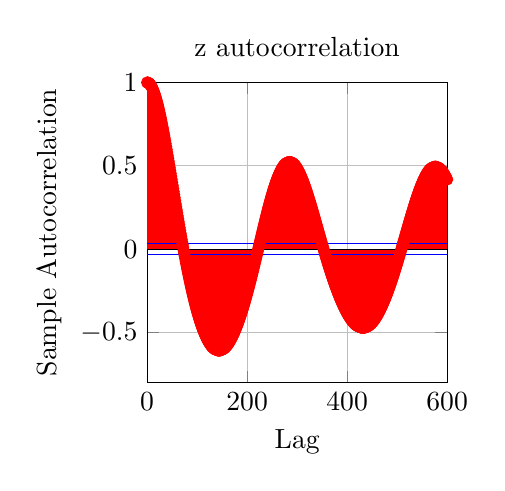
\begin{tikzpicture}

\begin{axis}[%
width=1.5in,
height=1.5in,
scale only axis,
xmin=0,
xmax=600,
xlabel={Lag},
xmajorgrids,
ymin=-0.8,
ymax=1,
ylabel={Sample Autocorrelation},
ymajorgrids,
title={z autocorrelation}
]
\addplot[ycomb,color=red,solid,mark size=2.0pt,mark=*,mark options={solid,fill=red}] plot table[row sep=crcr] {%
0	1\\
1	0.999547312698472\\
2	0.998480704944451\\
3	0.996801583574792\\
4	0.994512195560718\\
5	0.99161562106265\\
6	0.988115763762079\\
7	0.984017338529863\\
8	0.979325856506434\\
9	0.974047607684763\\
10	0.968189641101421\\
11	0.961759742754538\\
12	0.954766411379849\\
13	0.947218832227104\\
14	0.939126848988977\\
15	0.930500934043032\\
16	0.921352157174318\\
17	0.91169215295175\\
18	0.901533086935478\\
19	0.890887620895105\\
20	0.879768877219744\\
21	0.868190402700694\\
22	0.856166131865896\\
23	0.843710350042411\\
24	0.830837656319081\\
25	0.81756292657624\\
26	0.803901276743061\\
27	0.789868026435931\\
28	0.775478663123127\\
29	0.760748806952365\\
30	0.745694176368391\\
31	0.730330554637925\\
32	0.714673757389056\\
33	0.698739601261688\\
34	0.682543873754973\\
35	0.66610230434699\\
36	0.64943053695122\\
37	0.632544103763885\\
38	0.615458400545851\\
39	0.598188663372772\\
40	0.580749946877487\\
41	0.563157103999362\\
42	0.545424767246511\\
43	0.527567331468458\\
44	0.509598938129079\\
45	0.491533461062408\\
46	0.473384493687262\\
47	0.455165337650618\\
48	0.436888992864173\\
49	0.418568148893723\\
50	0.400215177656663\\
51	0.381842127379272\\
52	0.363460717762272\\
53	0.34508233630057\\
54	0.32671803570103\\
55	0.308378532340505\\
56	0.290074205705266\\
57	0.271815098752271\\
58	0.253610919132423\\
59	0.235471041216081\\
60	0.217404508861505\\
61	0.199420038867662\\
62	0.181526025053846\\
63	0.163730542909845\\
64	0.146041354761852\\
65	0.128465915401018\\
66	0.11101137812338\\
67	0.0936846011318592\\
68	0.0764921542531232\\
69	0.0594403259242666\\
70	0.0425351304065051\\
71	0.0257823151853536\\
72	0.00918736851906191\\
73	-0.00724447290060235\\
74	-0.0235082162088352\\
75	-0.0395991045808676\\
76	-0.0555126094267051\\
77	-0.0712444225944113\\
78	-0.0867904486066636\\
79	-0.102146796953223\\
80	-0.117309774459947\\
81	-0.13227587775304\\
82	-0.147041785835371\\
83	-0.161604352789932\\
84	-0.175960600623802\\
85	-0.19010771226443\\
86	-0.204043024718497\\
87	-0.217764022402251\\
88	-0.231268330650871\\
89	-0.244553709413185\\
90	-0.257618047136949\\
91	-0.270459354848814\\
92	-0.283075760432188\\
93	-0.29546550310527\\
94	-0.307626928100782\\
95	-0.319558481548173\\
96	-0.331258705558429\\
97	-0.342726233511068\\
98	-0.353959785542363\\
99	-0.364958164233417\\
100	-0.375720250496322\\
101	-0.386244999656304\\
102	-0.396531437727501\\
103	-0.40657865787977\\
104	-0.416385817093765\\
105	-0.425952133001371\\
106	-0.435276880908475\\
107	-0.444359390996989\\
108	-0.453199045702995\\
109	-0.461795277267844\\
110	-0.470147565459051\\
111	-0.478255435457822\\
112	-0.48611845591008\\
113	-0.49373623713785\\
114	-0.501108429507912\\
115	-0.508234721954615\\
116	-0.515114840653753\\
117	-0.521748547844406\\
118	-0.528135640795565\\
119	-0.534275950914348\\
120	-0.540169342992486\\
121	-0.545815714587629\\
122	-0.551214995535875\\
123	-0.556367147591681\\
124	-0.561272164191093\\
125	-0.565930070333897\\
126	-0.570340922579959\\
127	-0.574504809154613\\
128	-0.578421850157514\\
129	-0.582092197868871\\
130	-0.585516037146442\\
131	-0.588693585906123\\
132	-0.591625095678336\\
133	-0.594310852231846\\
134	-0.59675117625599\\
135	-0.598946424091719\\
136	-0.60089698850126\\
137	-0.602603299465674\\
138	-0.604065824999094\\
139	-0.605285071968071\\
140	-0.606261586904116\\
141	-0.606995956797412\\
142	-0.607488809859612\\
143	-0.607740816243817\\
144	-0.607752688710149\\
145	-0.607525183225862\\
146	-0.607059099489696\\
147	-0.60635528137113\\
148	-0.60541461725639\\
149	-0.604238040294451\\
150	-0.602826528537918\\
151	-0.601181104975451\\
152	-0.599302837454393\\
153	-0.597192838494348\\
154	-0.594852264994725\\
155	-0.592282317841471\\
156	-0.589484241420585\\
157	-0.586459323048202\\
158	-0.583208892329251\\
159	-0.579734320458699\\
160	-0.576037019481243\\
161	-0.57211844152693\\
162	-0.567980078041482\\
163	-0.563623459031153\\
164	-0.559050152342558\\
165	-0.554261762998253\\
166	-0.54925993260875\\
167	-0.544046338881181\\
168	-0.538622695244034\\
169	-0.532990750606192\\
170	-0.527152289267018\\
171	-0.521109130992476\\
172	-0.514863131270257\\
173	-0.508416181754666\\
174	-0.501770210909705\\
175	-0.494927184856328\\
176	-0.487889108427393\\
177	-0.480658026431352\\
178	-0.473236025123339\\
179	-0.465625233879988\\
180	-0.45782782707218\\
181	-0.449846026127871\\
182	-0.441682101775393\\
183	-0.433338376455962\\
184	-0.424817226892788\\
185	-0.416121086802975\\
186	-0.407252449737469\\
187	-0.398213872033551\\
188	-0.389007975863859\\
189	-0.379637452365536\\
190	-0.370105064832912\\
191	-0.360413651957101\\
192	-0.350566131095942\\
193	-0.340565501557928\\
194	-0.330414847884001\\
195	-0.320117343111458\\
196	-0.309676252004557\\
197	-0.29909493423685\\
198	-0.288376847510671\\
199	-0.277525550599653\\
200	-0.266544706300543\\
201	-0.255438084281011\\
202	-0.244209563810512\\
203	-0.23286313636162\\
204	-0.221402908069585\\
205	-0.209833102038147\\
206	-0.198158060479922\\
207	-0.186382246679918\\
208	-0.17451024677095\\
209	-0.162546771309929\\
210	-0.150496656644199\\
211	-0.138364866057265\\
212	-0.126156490683433\\
213	-0.113876750181083\\
214	-0.101530993154471\\
215	-0.0891246973141687\\
216	-0.0766634693665093\\
217	-0.0641530446226162\\
218	-0.0515992863179415\\
219	-0.039008184633539\\
220	-0.0263858554106805\\
221	-0.0137385385508585\\
222	-0.00107259609367459\\
223	0.0116054900343443\\
224	0.0242891206063846\\
225	0.0369715820231797\\
226	0.0496460495870797\\
227	0.0623055911266391\\
228	0.0749431709751891\\
229	0.0875516543059881\\
230	0.100123811825612\\
231	0.112652324826263\\
232	0.125129790596645\\
233	0.137548728189962\\
234	0.149901584546489\\
235	0.162180740966976\\
236	0.174378519931971\\
237	0.186487192260911\\
238	0.198498984603576\\
239	0.210406087255252\\
240	0.222200662285651\\
241	0.233874851970382\\
242	0.245420787512473\\
243	0.256830598040189\\
244	0.268096419866141\\
245	0.279210405991463\\
246	0.290164735837641\\
247	0.30095162518742\\
248	0.311563336315131\\
249	0.321992188285681\\
250	0.332230567400511\\
251	0.342270937767829\\
252	0.35210585197361\\
253	0.361727961829022\\
254	0.371130029169255\\
255	0.380304936678052\\
256	0.389245698711744\\
257	0.397945472096059\\
258	0.406397566868672\\
259	0.414595456940108\\
260	0.422532790645471\\
261	0.430203401159326\\
262	0.437601316746086\\
263	0.444720770818315\\
264	0.451556211775521\\
265	0.458102312596312\\
266	0.46435398015708\\
267	0.470306364250861\\
268	0.475954866280505\\
269	0.481295147600892\\
270	0.486323137485622\\
271	0.491035040694335\\
272	0.49542734461765\\
273	0.499496825977632\\
274	0.503240557062608\\
275	0.506655911476238\\
276	0.509740569381797\\
277	0.512492522223809\\
278	0.514910076910349\\
279	0.516991859440647\\
280	0.518736817963897\\
281	0.520144225256587\\
282	0.521213680607074\\
283	0.521945111097599\\
284	0.522338772275473\\
285	0.522395248206705\\
286	0.522115450906964\\
287	0.521500619146408\\
288	0.520552316626595\\
289	0.519272429529395\\
290	0.51766316343959\\
291	0.515727039644596\\
292	0.513466890816547\\
293	0.510885856083811\\
294	0.507987375500779\\
295	0.504775183926686\\
296	0.501253304325956\\
297	0.497426040504495\\
298	0.493297969298079\\
299	0.488873932230854\\
300	0.484159026663692\\
301	0.479158596453894\\
302	0.473878222149427\\
303	0.468323710742507\\
304	0.462501085008924\\
305	0.456416572461013\\
306	0.450076593943584\\
307	0.443487751903489\\
308	0.436656818364714\\
309	0.429590722642053\\
310	0.422296538827417\\
311	0.414781473083762\\
312	0.407052850782376\\
313	0.399118103519934\\
314	0.390984756052226\\
315	0.382660413181839\\
316	0.374152746637299\\
317	0.365469481981253\\
318	0.356618385585209\\
319	0.347607251708104\\
320	0.338443889715649\\
321	0.329136111476817\\
322	0.319691718973226\\
323	0.310118492156337\\
324	0.300424177086429\\
325	0.29061647438625\\
326	0.280703028041007\\
327	0.270691414575026\\
328	0.260589132633946\\
329	0.250403592999764\\
330	0.240142109064335\\
331	0.229811887785193\\
332	0.219420021145682\\
333	0.208973478139449\\
334	0.198479097297347\\
335	0.187943579772703\\
336	0.177373482998795\\
337	0.166775214930187\\
338	0.156155028877372\\
339	0.145519018941917\\
340	0.134873116057043\\
341	0.124223084636301\\
342	0.113574519830712\\
343	0.102932845392465\\
344	0.092303312141013\\
345	0.0816909970251519\\
346	0.0711008027724393\\
347	0.0605374581151623\\
348	0.0500055185798954\\
349	0.0395093678256305\\
350	0.0290532195134246\\
351	0.0186411196885698\\
352	0.00827694965440519\\
353	-0.00203557068489241\\
354	-0.0122928790369061\\
355	-0.0224915665149225\\
356	-0.0326283730406701\\
357	-0.0427001823846691\\
358	-0.0527040168742564\\
359	-0.0626370318004601\\
360	-0.072496509555878\\
361	-0.0822798535365362\\
362	-0.0919845818413852\\
363	-0.10160832080361\\
364	-0.111148798388279\\
365	-0.120603837491063\\
366	-0.129971349172753\\
367	-0.139249325864165\\
368	-0.14843583457569\\
369	-0.157529010145251\\
370	-0.166527048557734\\
371	-0.175428200368139\\
372	-0.184230764259668\\
373	-0.192933080766786\\
374	-0.201533526191983\\
375	-0.210030506743455\\
376	-0.218422452919313\\
377	-0.226707814162196\\
378	-0.234885053806252\\
379	-0.242952644336529\\
380	-0.250909062978715\\
381	-0.258752787635037\\
382	-0.266482293179914\\
383	-0.274096048126717\\
384	-0.281592511674705\\
385	-0.288970131142887\\
386	-0.296227339795288\\
387	-0.303362555059815\\
388	-0.310374177140646\\
389	-0.317260588021922\\
390	-0.324020150858331\\
391	-0.330651209746158\\
392	-0.337152089866402\\
393	-0.34352109798967\\
394	-0.349756523330847\\
395	-0.355856638739853\\
396	-0.361819702213342\\
397	-0.367643958710754\\
398	-0.373327642256958\\
399	-0.378868978312534\\
400	-0.384266186391851\\
401	-0.38951748290818\\
402	-0.394621084224448\\
403	-0.399575209887614\\
404	-0.40437808602422\\
405	-0.409027948874348\\
406	-0.413523048440976\\
407	-0.417861652231647\\
408	-0.42204204906933\\
409	-0.426062552949453\\
410	-0.429921506920272\\
411	-0.433617286963987\\
412	-0.437148305856338\\
413	-0.440513016982877\\
414	-0.443709918090525\\
415	-0.446737554953638\\
416	-0.449594524934411\\
417	-0.452279480418127\\
418	-0.454791132104583\\
419	-0.457128252137839\\
420	-0.459289677057399\\
421	-0.461274310554974\\
422	-0.463081126022099\\
423	-0.464709168875126\\
424	-0.46615755864545\\
425	-0.467425490824318\\
426	-0.468512238453109\\
427	-0.469417153451725\\
428	-0.470139667679499\\
429	-0.470679293724998\\
430	-0.471035625423083\\
431	-0.471208338099753\\
432	-0.471197188547441\\
433	-0.471002014735711\\
434	-0.470622735264541\\
435	-0.470059348569665\\
436	-0.469311931891648\\
437	-0.468380640022571\\
438	-0.467265703846218\\
439	-0.465967428689627\\
440	-0.464486192505576\\
441	-0.462822443907159\\
442	-0.460976700076889\\
443	-0.45894954457384\\
444	-0.456741625063084\\
445	-0.454353650992167\\
446	-0.451786391239531\\
447	-0.449040671759616\\
448	-0.446117373248954\\
449	-0.443017428856802\\
450	-0.439741821962825\\
451	-0.436291584043074\\
452	-0.43266779264398\\
453	-0.428871569482394\\
454	-0.424904078687809\\
455	-0.420766525200947\\
456	-0.416460153340773\\
457	-0.411986245549914\\
458	-0.407346121326274\\
459	-0.402541136346543\\
460	-0.3975726817852\\
461	-0.392442183830612\\
462	-0.387151103397905\\
463	-0.3817009360365\\
464	-0.376093212028493\\
465	-0.370329496672536\\
466	-0.364411390746426\\
467	-0.358340531140353\\
468	-0.352118591651541\\
469	-0.345747283930047\\
470	-0.339228358564473\\
471	-0.3325636062956\\
472	-0.325754859345149\\
473	-0.318803992846258\\
474	-0.311712926361704\\
475	-0.304483625475316\\
476	-0.297118103441662\\
477	-0.289618422878609\\
478	-0.281986697487079\\
479	-0.274225093781995\\
480	-0.266335832818225\\
481	-0.258321191895173\\
482	-0.250183506223622\\
483	-0.241925170538507\\
484	-0.233548640641477\\
485	-0.225056434857455\\
486	-0.216451135389965\\
487	-0.207735389560738\\
488	-0.198911910920112\\
489	-0.189983480216056\\
490	-0.180952946211245\\
491	-0.171823226339553\\
492	-0.162597307195699\\
493	-0.15327824485445\\
494	-0.143869165018924\\
495	-0.134373263001056\\
496	-0.124793803541157\\
497	-0.115134120477764\\
498	-0.105397616283502\\
499	-0.0955877614874482\\
500	-0.0857080940093899\\
501	-0.0757622184362174\\
502	-0.0657538052754941\\
503	-0.0556865902256351\\
504	-0.0455643735060706\\
505	-0.0353910192939648\\
506	-0.0251704553163328\\
507	-0.0149066726474869\\
508	-0.00460372576145931\\
509	0.00573426711282519\\
510	0.0161031232895048\\
511	0.0264985945382615\\
512	0.0369163655802322\\
513	0.0473520521457226\\
514	0.0578011985834624\\
515	0.0682592750242494\\
516	0.0787216741164142\\
517	0.0891837073662696\\
518	0.099640601133144\\
519	0.110087492345254\\
520	0.120519424018963\\
521	0.130931340679341\\
522	0.141318083793736\\
523	0.151674387341783\\
524	0.161994873654271\\
525	0.172274049659249\\
526	0.182506303676209\\
527	0.192685902897973\\
528	0.202806991694983\\
529	0.212863590868061\\
530	0.222849597963597\\
531	0.23275878874994\\
532	0.24258481993593\\
533	0.25232123319259\\
534	0.261961460517662\\
535	0.271498830960579\\
536	0.280926578703249\\
537	0.290237852470405\\
538	0.29942572622277\\
539	0.308483211067438\\
540	0.317403268303108\\
541	0.326178823503422\\
542	0.334802781529834\\
543	0.34326804235633\\
544	0.351567517581846\\
545	0.359694147502335\\
546	0.367640918612978\\
547	0.375400881411683\\
548	0.382967168377626\\
549	0.390333012002783\\
550	0.397491762759858\\
551	0.404436906896538\\
552	0.411162083953149\\
553	0.417661103908471\\
554	0.42392796386627\\
555	0.429956864202993\\
556	0.435742224104764\\
557	0.441278696429258\\
558	0.446561181835079\\
559	0.451584842127903\\
560	0.45634511277881\\
561	0.460837714575913\\
562	0.465058664375633\\
563	0.469004284924744\\
564	0.472671213728741\\
565	0.476056410946106\\
566	0.479157166291805\\
567	0.481971104936869\\
568	0.484496192394219\\
569	0.486730738384042\\
570	0.488673399675144\\
571	0.490323181901666\\
572	0.491679440357575\\
573	0.492741879774309\\
574	0.49351055308997\\
575	0.493985859221505\\
576	0.494168539854399\\
577	0.494059675267534\\
578	0.493660679214037\\
579	0.492973292882127\\
580	0.491999577963206\\
581	0.490741908857602\\
582	0.489202964051611\\
583	0.487385716702584\\
584	0.485293424471883\\
585	0.482929618648523\\
586	0.480298092609128\\
587	0.477402889662585\\
588	0.474248290330265\\
589	0.470838799115052\\
590	0.467179130814521\\
591	0.463274196435499\\
592	0.459129088768858\\
593	0.454749067684746\\
594	0.450139545209518\\
595	0.445306070446413\\
596	0.440254314402452\\
597	0.434990054784202\\
598	0.429519160824864\\
599	0.423847578204683\\
600	0.417981314125813\\
};
\addplot [color=blue,solid,forget plot]
  table[row sep=crcr]{%
0.5	0.0346427483320998\\
600	0.0346427483320998\\
};
\addplot [color=blue,solid,forget plot]
  table[row sep=crcr]{%
0.5	-0.0346427483320998\\
600	-0.0346427483320998\\
};
\addplot [color=black,solid,forget plot]
  table[row sep=crcr]{%
0	0\\
600	0\\
};
\end{axis}
\end{tikzpicture}%
\end{document}
\caption{Autocorrelation of the flattened three dimensional as well as x,y and z related training data sets.}
\label{fig:lorAutocorr}
\end{figure}
The comparison of the flattened autocorrelation with the single dimension couterparts shown in figure~\ref{fig:lorAutocorr} reveals that possibly the three dimensions are best treated separately.
Therefore an attempt to train a Lorenz svm committee-network has been made. One svm per dimension is trained, which means one svm per Lorenz equation. The current version of the \texttt{lssvm toolbox} requires an \texttt{X : N x d matrix with the inputs of the training data} as well as an \texttt{Y : N x 1 vector with the outputs of the training data}. \footnote{LS-SVMlab Toolbox User’s Guide
version 1.8, K. De Brabanter et al. page 104, \url{http://www.esat.kuleuven.be/sista/lssvmlab/downloads/tutorialv1_8.pdf}} Which means no tensor inputs are allowed. As the columns of the input are required for the windowing a flattened version of the 3 dimensional input has to be used as a workaround. In order to meet the length requirement the unwanted dimensions of the output have been padded with zeros. The flattened predictions have then been added up and reshaped into their original three dimensional form. But unfortunately this approach did not improve results. This is probably due to the fact that zero padding the unwanted output dimensions introduces new false information, from which the Committee-network does not recover. 


